\documentclass[twoside]{article}
\usepackage{epsfig,html,amsmath,amssymb,lscape,longtable,pstricks,hyperref}
\pagestyle{headings}
\markboth{}{}
\begin{document}
\title{CalculiX CrunchiX USER'S MANUAL development version}
\author{Guido Dhondt}
\maketitle
\tableofcontents
\section{Introduction.}
This is a description of CalculiX CrunchiX. If you have any problems using the
program, this document should solve them. If not, send us an E-mail
(dhondt@t-online.de). The next sections contain some useful information on how
to use CalculiX in parallel, hints about units and golden rules you should
always keep in mind before starting an analysis. Section five contains a simple example problems to
wet your appetite. Section six is a theoretical section giving some
background on the analysis types, elements, materials etc. Then, an overview
is given of all the available keywords in alphabetical order, followed by
detailed instructions on the format of the input deck. If CalculiX does not
run because your input deck has problems, this is the section to look
at. Then, there is a section on the user subroutines and a short overview of
the program structure. The CalculiX distribution contains a large set of test
examples (CalculiX.test.tar.bz2).  If you try to solve a
new kind of problem you haven't dealt with in the past, check these
examples. You can also use them to check whether you installed
CalculiX correctly (if you do so with the compare script and if you experience
problems with some of the examples, please check the comments at the start of
the corresponding input deck). Finally, the User's Manual ends with some references used while writing the code.

This manual is not a textbook on finite elements. Indeed, a working knowledge
of the Finite Element Method is assumed. For people not familiar with the
Finite Element Method, I recommend the book by Zienkiewicz and Taylor
\cite{Zienkiewicz} for engineering oriented students and the publications by
Hughes \cite{Hughes} and Dhondt \cite{Dhondt} for mathematically minded
readers.

\section{How to perform CalculiX calculations in parallel \label{parallel}}

Nowadays most computers have one socket with several cores, allowing for the calculations to be
performed in a parallel way. In CalculiX one can 

\begin{itemize}
\item create the element stiffness matrices in parallel. No special compilation flag is needed. At execution
  time the environment variable OMP\_NUM\_THREADS or the environment variable CCX\_NPROC\_STIFFNESS must be set to the number of cores,
  default is 1. If both are set, CCX\_NPROC\_STIFFNESS takes
  precedence. The maximum number of cores is detected automatically by CalculiX
  by using
  the sysconf(\_SC\_NPROCESSORS\_CONF) function. It can be overriden by the
  user by means of environment variable NUMBER\_OF\_CPUS.

  Notice that older GNU-compiler versions (e.g. gcc 4.2.1) may have problems with this
  parallellization due to the size of the fields to be allocated within each
  thread (e.g. s(100,100) in routine e\_3d.f). This should not be a problem
  with the actual compiler version.

\item solve the system of equations with the multithreaded version of
  SPOOLES. To this end

\begin{itemize}
\item the MT-version of SPOOLES must have been compiled. For further
  information on this topic please consult the SPOOLES documentation
\item CalculiX CrunchiX must have been compiled with the USE\_MT flag activated
  in the Makefile, please consult the README.INSTALL file.
\item at execution time the environment variable OMP\_NUM\_THREADS must have been set to the number of
  cores you want to use. In Linux this can be done by ``export OMP\_NUM\_THREADS=n'' on
  the command line, where n is the number of cores. Default is
  1. Alternatively, you can set the number of cores using the environment
  variable CCX\_NPROC\_EQUATION\_SOLVER. If both are set, the latter takes
  precedence. 
\end{itemize} 

\item solve the system of equations with the multithreaded version of
  PARDISO. PARDISO is proprietary. Look at the PARDISO documentation how to link the
  multithreaded version. At execution
  time the environment variable OMP\_NUM\_THREADS must be set to the number of cores,
  default is 1.

\item create material tangent matrices and calculate the stresses at the
  integration points in parallel. No special compilation flag is needed. At execution
  time the environment variable OMP\_NUM\_THREADS or the environment variable CCX\_NPROC\_RESULTS must be set to the number of cores,
  default is 1. If both are set, CCX\_NPROC\_RESULTS takes
  precedence. The maximum number of cores is detected automatically by CalculiX
  by using
  the sysconf(\_SC\_NPROCESSORS\_CONF) function. It can be overriden by the
  user by means of environment variable NUMBER\_OF\_CPUS. Notice that if a
  material user subroutine (Sections \ref{user} and \ref{thuser}) is used, certain rules have to be complied with in
  order to allow parallelization. These include (this list is possibly not exhaustive):
\begin{itemize}
\item no save statements
\item no data statements
\item avoid logical variables
\item no write statements
\end{itemize}

\item calculate the viewfactors for thermal radiation computations in parallel. No special compilation flag is needed. At execution
  time the environment variable OMP\_NUM\_THREADS or the environment variable CCX\_NPROC\_VIEWFACTOR must be set to the number of cores,
  default is 1. If both are set, CCX\_NPROC\_VIEWFACTOR takes precedence. The maximum number of cores is detected automatically by CalculiX by using
  the sysconf(\_SC\_NPROCESSORS\_CONF) function. It can be overriden by the
  user by means of environment variable NUMBER\_OF\_CPUS.

\item perform several operations in CFD calculations (computational fluid
  dynamics) in parallel. No special compilation flag is needed. At execution
  time the environment variable OMP\_NUM\_THREADS or the environment variable CCX\_NPROC\_CFD must be set to the number of cores,
  default is 1. If both are set, CCX\_NPROC\_CFD takes precedence. The maximum number of cores is detected automatically by CalculiX by using
  the sysconf(\_SC\_NPROCESSORS\_CONF) function. It can be overriden by the
  user by means of environment variable NUMBER\_OF\_CPUS.

\item Calculate the magnetic intensity by use of the Biot-Savart law in parallel. No special compilation flag is needed. At execution
  time the environment variable OMP\_NUM\_THREADS or the environment variable CCX\_NPROC\_BIOTSAVART must be set to the number of cores,
  default is 1. If both are set, CCX\_NPROC\_BIOTSAVART takes precedence. The maximum number of cores is detected automatically by CalculiX by using
  the sysconf(\_SC\_NPROCESSORS\_CONF) function. It can be overriden by the
  user by means of environment variable NUMBER\_OF\_CPUS.

\item Perform several vector and matrix operations needed by the SLATEC
  iterative solvers or by ARPACK in parallel. To this end the user must have
  defined the environment variable OMP\_NUM\_THREADS, and used the openmp
  FORTRAN flag in the Makefile. The parallellization is done in FORTRAN
  routines using openmp. The corresponding lines start with ``c\$omp''. If the
  openmp flag is not used, these lines are interpreted by the compiler as comment lines and no
  parallellization takes place. Notice that this parallellization only pays
  off for rather big systems, let's say 300,000 degrees of freedom for
  CFD-calculations or 1,000,000 degrees of freedom for mechanical frequency calculations.
 
\end{itemize}

Examples:
\begin{itemize}
\item For some reason the function sysconf does not work on your computer
  system and leads to a segmentation fault. You can prevent using the function
  by defining the maximum number of cores explicitly using the NUMBER\_OF\_CPUS
  environment variable
\item You want to perform a thermomechanical calculation, but you are using a
  user defined material subroutine (Sections \ref{user} and \ref{thuser}) which is not suitable for
  parallelization. You can make maximum use of parallelization (e.g. for the
  calculation of viewfactors) by setting the
  variable OMP\_NUM\_THREADS to the maximum number of cores on your system, and
  prevent parallelization of the material tangent and stress calculation step by setting
  CCX\_NPROC\_RESULTS to 1.
\end{itemize}



\section{Units}

An important issue which frequently raises questions concerns units. Finite element
programs do not know any units. The user has to take care of that. In fact,
there is only one golden rule: the user must make sure that the numbers he
provides have consistent units. The number of units one
can freely choose depends on the application. For thermomechanical problems you
can choose four units, e.g. for length, mass, time and temperature. If these
are chosen, everything else is fixed. If you choose SI units for these
quantities, i.e. $\text{m}$ for length, $\text{kg}$ for mass, $\text{s}$ for time and $\text{K}$ for temperature,
force will be in $\text{kg}\text{m}/\text{s}^2 = \text{N}$, pressure will be
in $\text{N}/\text{m}^2 = \text{kg}/\text{m}\text{s}^2$, density will be in
$\text{kg}/\text{m}^3$, thermal conductivity in $\text{W}/\text{m}\text{K} =
\text{J}/\text{s}\text{m}\text{K} =
\text{N}\text{m}/\text{s}\text{m}\text{K} =
\text{kg}\text{m}^2/\text{s}^3\text{m}\text{K} =
\text{kg}\text{m}/\text{s}^3\text{K}$ , specific heat in
$\text{J}/\text{kg}\text{K} = \text{N}\text{m}/\text{kg}\text{K} =
\text{m}^2/\text{s}^2\text{K}$ and so on. The density of steel in the SI
system is 7800 $\text{kg}/\text{m}^3$.

If you choose $\text{mm}$ for length, $\text{g}$ for mass, $\text{s}$ for time
and $\text{K}$ for temperature, force will be in
$\text{g}\text{mm}/\text{s}^2$ and thermal conductivity in
$\text{g}\text{mm}/\text{s}^3\text{K}$. In the
$\{\text{mm},\text{g},\text{s},\text{K}\}$ system the density of steel is $7.8
\times 10^{-3}$ since $7800 \text{kg}/\text{m}^3 = 7800 \times 10^{-6}
\text{g}/\text{mm}^3$. 

However, you can also choose other quantities as the independent ones. A
popular system at my company is $\text{mm}$ for length, $\text{N}$ for force,
$\text{s}$ for time and $\text{K}$ for temperature. Now, since force = mass
$\times$ length / $\text{time}^2$, we get that mass = force $\times$ $
\text{time}^2$/length. This leads to $\text{N}\text{s}^2/\text{mm}$ for the mass
and $\text{N}\text{s}^2/\text{mm}^4$ for density. This means that in the
$\{\text{mm}, \text{N}, \text{s}, \text{K} \}$ system the density of steel is
$7.8 \times 10^{-9}$ since $7800 \text{kg}/\text{m}^3 = 7800
\text{N}\text{s}^2/\text{m}^4 = 7.8 \times 10^{-9}
\text{N}\text{s}^2/\text{mm}^4$. 

Notice that your are not totally free in choosing the four basic units: you
cannot choose the unit of force, mass, length and time as basic units since
they are linked with each other through force = mass $\times$ length /
$\text{time}^2$. 

Finally, a couple of additional examples. Young's Modulus for steel is $210000
\text{N}/ \text{mm}^2 = 210000 \times 10^6 \text{N}/\text{m}^2 = 210000 \times
10^6 \text{kg}/\text{m}\text{s}^2 = 210000 \times 10^6
\text{g}/\text{mm}\text{s}^2 $. So its value in the SI system is $210 \times
10^9$, in the $\{\text{mm},\text{g},\text{s},\text{K}\}$ system it is also
$210 \times 10^9$ and in the $\{\text{mm}, \text{N}, \text{s}, \text{K} \}$
system it is $210 \times 10^3$. The heat capacity of steel is $446
\text{J}/\text{kg}\text{K} = 446 \text{m}^2/\text{s}^2\text{K} = 446 \times
10^6 \text{mm}^2/\text{s}^2\text{K}$, so in the SI system it is $446.$, in the 
$\{\text{mm},\text{g},\text{s},\text{K}\}$  and $\{\text{mm}, \text{N},
\text{s}, \text{K} \}$ system it is $446 \times 10^6$.

Table \ref{units} gives an overview of frequently used units in three
different systems: the $\{\text{m}, \text{kg},
\text{s}, \text{K} \}$ system, the $\{\text{mm}, \text{N},
\text{s}, \text{K} \}$ system and the $\{\text{cm}, \text{g},
\text{s}, \text{K} \}$ system.

\begin{table}
\caption{Frequently used units in different unit systems.\label{units}}
\begin{center}
\begin{tabular}{|c|c|c|c|c|}
\hline
 symbol & meaning & m,kg,s,K & mm,N,s,K & cm,g,s,K\\
\hline
& & & & \\
E & Young's Modulus &  $1 \frac{N}{m^2 } = 1 \frac{kg}{m s^2 }$ & $= 10^{-6}
\frac{N}{mm^2 }$ & $= 1 \frac{g}{mm s^2 }$ \\
& & & & \\
$\rho$ & Density & 1 $\frac{kg}{m^3 } $ & $= 10^{-12}
\frac{Ns^2}{mm^4 }$ & $= 10^{-6} \frac{g}{mm^3 }$ \\
& & & & \\
F & Force &  $1 N = 1 \frac{kg m}{ s^2 }$ & $= 1
N$ & $= 10^{6} \frac{g\: mm}{s^2 }$ \\
& & & & \\
$c_p$ & Specific Heat &  $1 \frac{J}{kg K} = 1 \frac{m^2}{ s^2 K}$ & $= 10^{6}
\frac{mm^2}{s^2 K }$ & $= 10^6 \frac{mm^2}{s^2 K }$ \\
& & & & \\
$\lambda$ & Conductivity & 1 $\frac{W}{m K } = 1 \frac{kg m}{s^3 K }$ & $= 1
\frac{N}{s K }$ & $= 10^6 \frac{g\: mm}{s^3 K}$ \\
& & & & \\
h & Film Coefficient &  $1 \frac{W}{m^2 K } = 1 \frac{kg}{s^3 K }$ & $= 10^{-3}
\frac{N}{mm\: s K }$ & $= 10^3 \frac{g}{s^3 K }$ \\
& & & & \\
$\mu$ & Dynamic Viscosity &  $1 \frac{N s}{m^2 } = 1 \frac{kg}{m s }$ & $= 10^{-6}
\frac{N s}{mm^2 }$ & $= 1 \frac{g}{mm\: s }$ \\
& & & & \\
\hline
\end{tabular}
\end{center}        
\end{table}

Typical values for air, water and steel at room temperature are:

\begin{itemize}
\item air
\begin{itemize}
\item $c_p=1005 \:\text{J}/\text{kg}\text{K} = 1005 \times 10^6 \:\text{mm}^2/\text{s}^2\text{K}$
\item $\lambda = 0.0257 \:W/\text{m}\text{K} = 0.0257 \:\text{N}/\text{s}\text{K}$
\item $\mu=18.21 \times 10^{-6} \:\text{kg}/\text{m}\text{s} = 18.21 \times 10^{-12} \:\text{N}\text{s}/\text{mm}^2$
\item $r$ (specific gas constant) $= 287 \:\text{J}/\text{kg}\text{K} = 287 \times 10^6 \:\text{mm}^2/\text{s}^2\text{K}$
\end{itemize}
\item water
\begin{itemize}
\item $\rho=1000 \:\text{kg}/\text{m}^3 = 10^{-9} \:\text{N}\text{s}^2/\text{mm}^4$
\item $c_p=4181.8 \:\text{J}/\text{kg}\text{K} = 4181.8 \times 10^6 \:\text{mm}^2/\text{s}^2\text{K}$
\item $\lambda= 0.5984 \:W/\text{m}\text{K} = 0.5984 \:\text{N}/\text{s}\text{K}$
\item $\mu=10^{-3} \:\text{Pa}\:\text{s} = 10^{-9} \:\text{N}\text{s}/\text{mm}^2$
\end{itemize}
\item steel
\begin{itemize}
\item $E=210000 \time 10^6 \:\text{N}/\text{m}^2 = 210000 \:\text{N}/\text{mm}^2$
\item $\nu$ (Poisson coefficient)$ =0.3$
\item $\rho= 7800 \:\text{kg}/\text{m}^3=7.8 \times 10^{-9} \:\text{N}\text{s}^2/\text{mm}^4$
\item $c_p=446 \:\text{J}/\text{kg}\text{K} = 446 \times 10^6 \:\text{mm}^2/\text{s}^2\text{K}$
\item $\lambda=50 \:\text{W}/\text{m}\text{K} = 50 \:\text{N}/\text{s}\text{K}$
\end{itemize}
\end{itemize}

\section{Golden rules}

Applying the finite element method to real-life problems is not always a piece
of cake. Especially achieving convergence for nonlinear applications (large
deformation, nonlinear material behavior, contact) can be quite
tricky. However, adhering to a couple of simple rules can make life a lot
easier. According to my experience, the following guidelines are quite
helpful:

\begin{enumerate}
\item Check the quality of your mesh in CalculiX GraphiX or by using any other
  good preprocessor.

\item If you are dealing with a nonlinear problem, RUN A LINEARIZED VERSION FIRST: eliminate large deformations (drop NLGEOM), use a linear elastic
  material and drop all other nonlinearities such as contact. If the linear
  version doesn't run, the nonlinear problem won't run either. The linear
  version allows you to check easily whether the boundary conditions are
  correct (no unrestrained rigid body modes), the loading is the one you meant
  to apply etc. Furthermore, you get a feeling what the solution should look
  like.

\item USE QUADRATIC ELEMENTS (C3D10, C3D15, C3D20(R), S8, CPE8, CPS8, CAX8,
  B32), except for explicit dynamic calculations. The standard shape functions for quadratic elements are very
  good. Most finite element programs use these standard functions. For linear
  elements this is not the case: linear elements exhibit all kind of weird behavior such
  as shear locking and volumetric locking. Therefore, most finite element
  programs modify the standard shape functions for linear elements to
  alleviate these problems. However, there is no standard way of doing this,
  so each vendor has created his own modifications without necessarily
  publishing them. This leads to a larger variation in the results if you use
  linear elements. Since CalculiX uses the standard shape functions for linear
  elements too, the results must be considered with care.

\item If you are using shell elements or beam elements,
  use the option OUTPUT=3D on the *NODE FILE card in CalculiX (which is default). That way you
  get the expanded form of these elements in the .frd file. You can easily
  verify whether the thicknesses you specified are correct. Furthermore, you
  get the 3D stress distribution. It is the basis for the 1D/2D stress
  distribution and the internal beam forces. If the former is incorrect, so
  will the latter be.

\item If you include contact in your calculations and you are using quadratic
  elements, use the face-to-face penalty contact method or the mortar method
  (which is by default a face-to-face method). In general, for
  contact between faces the face-to-face penalty method and the mortar method will converge
  much better than the node-to-face method. The type of contact has to be
  declared on the \htmlref{*CONTACT PAIR}{contactpair} card. Notice that the
  mortar method in CalculiX can only be used for static calculations.

\item If you are performing an explicit dynamic calculation use:
  \begin{itemize}
  \item linear elements (C3D4, C3D8 or C3D6)
  \item node-to-face contact
  \item mass scaling: this is activated automatically as soon as you specify a
    minimum time increment (third entry underneath \htmlref{*DYNAMIC}{dynamic}).
  \end{itemize}
  
\item if you do not have enough space to run a problem, check the
  numbering. The memory needed to run a problem depends on the largest node
  and element numbers (the computational time, though, does not). So if you
  notice large gaps in the numbering, get rid of them and you will need less
  memory. In some problems you can save memory by choosing an iterative
  solution method. The iterative scaling method
  (cf. \htmlref{*STATIC}{static}) needs less memory than the iterative
  Cholesky method, the latter needs less memory than SPOOLES or PARDISO.
\end{enumerate}

If you experience problems you can:

\begin{enumerate}
\item look at the screen output. In particular, the convergence information
  for nonlinear calculations may indicate the source of your problem.

\item look at the .sta file. This file contains information on the number of
  iterations needed in each increment to obtain convergence

\item look at the .cvg file. This file is a synopsis of the screen output: it
  gives you a very fast overview of the number of contact elements, the
  residual force and the largest change in solution in each iteration (no
  matter whether convergent or not).

\item use the ``last iterations'' option on the \htmlref{*NODE FILE}{nodefile}
  or similar card. This generates a file with the name
  ResultsForLastIterations.frd with the deformation (for mechanical
  calculations) and the temperature (for thermal calculations) for all
  non-converged iterations starting after the last convergent increment.

\item if you have contact definitions in your input deck you may use the
  ``contact elements'' option on the \htmlref{*NODE FILE}{nodefile}
  or similar card. This generates a file with the name jobname.cel
  with all contact elements in all iterations of the increment in which this
  option is active. By reading this file in CalculiX GraphiX you can visualize
  all contact elements in each iteration and maybe find the source of your
  problems. 

\item if you experience a segmentation fault, you may set the environment
  variable CCX\_LOG\_ALLOC to 1 by typing ``export CCX\_LOG\_ALLOC=1'' in a
  terminal window. Running CalculiX you will get information on which fields
  are allocated, reallocated or freed at which line in the code (default is
  0).

\item this is for experts: if you experience problems with dependencies
  between different equations you can print the SPC's at the beginning of each
  step by removing the comment in front of the call to writeboun in CalculiX.c
  and recompile, and you can print the MPC's each time they are set up by
  decommenting the loop in which writempc is called at the beginning of
  cascade.c and recompile.
\end{enumerate}

\section{Simple example problems}

\subsection{Cantilever beam}

\begin{figure}
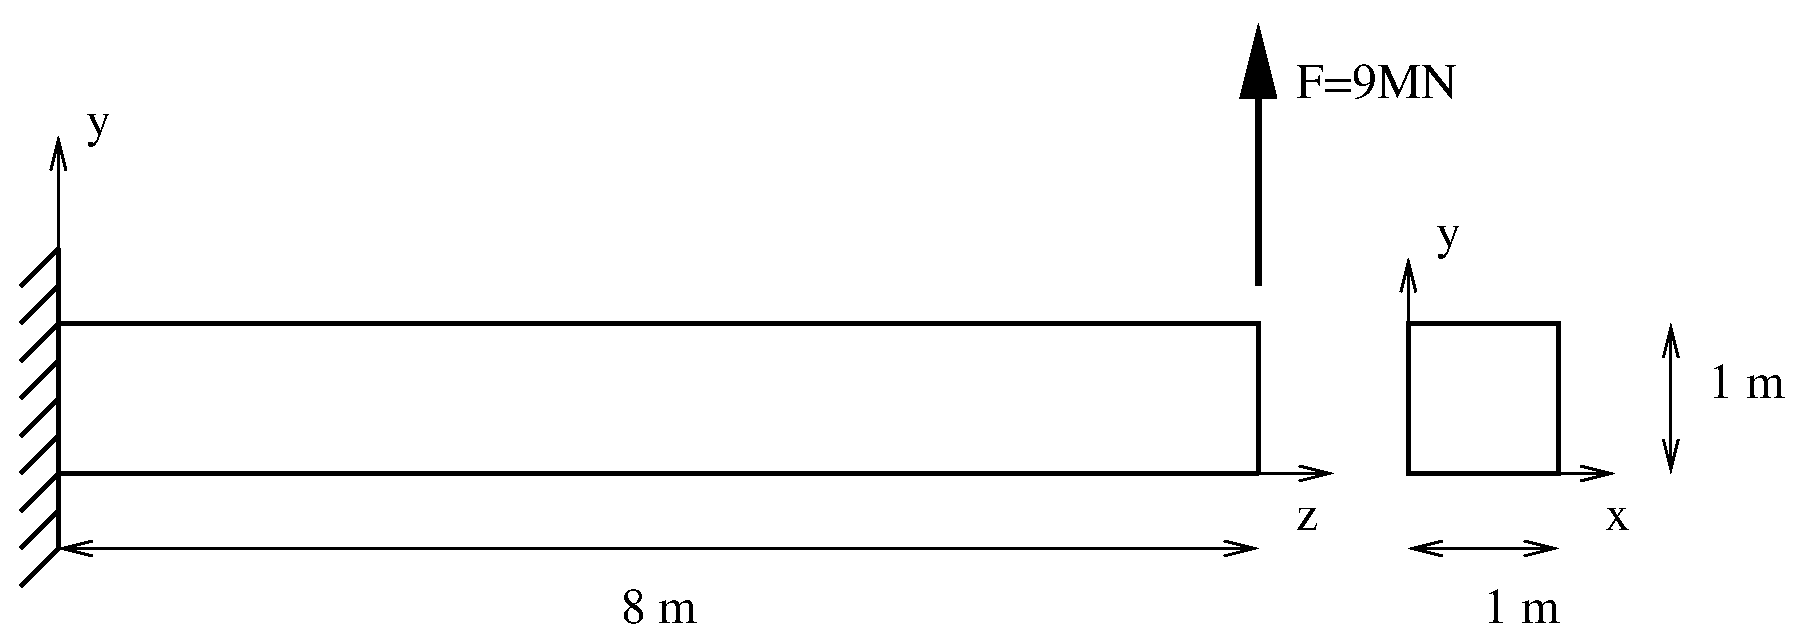
\epsfig{file=Beam1.eps,width=10cm}
\caption{\label{beam1}Geometry and boundary conditions of the beam problem}
\end{figure}

\begin{figure}
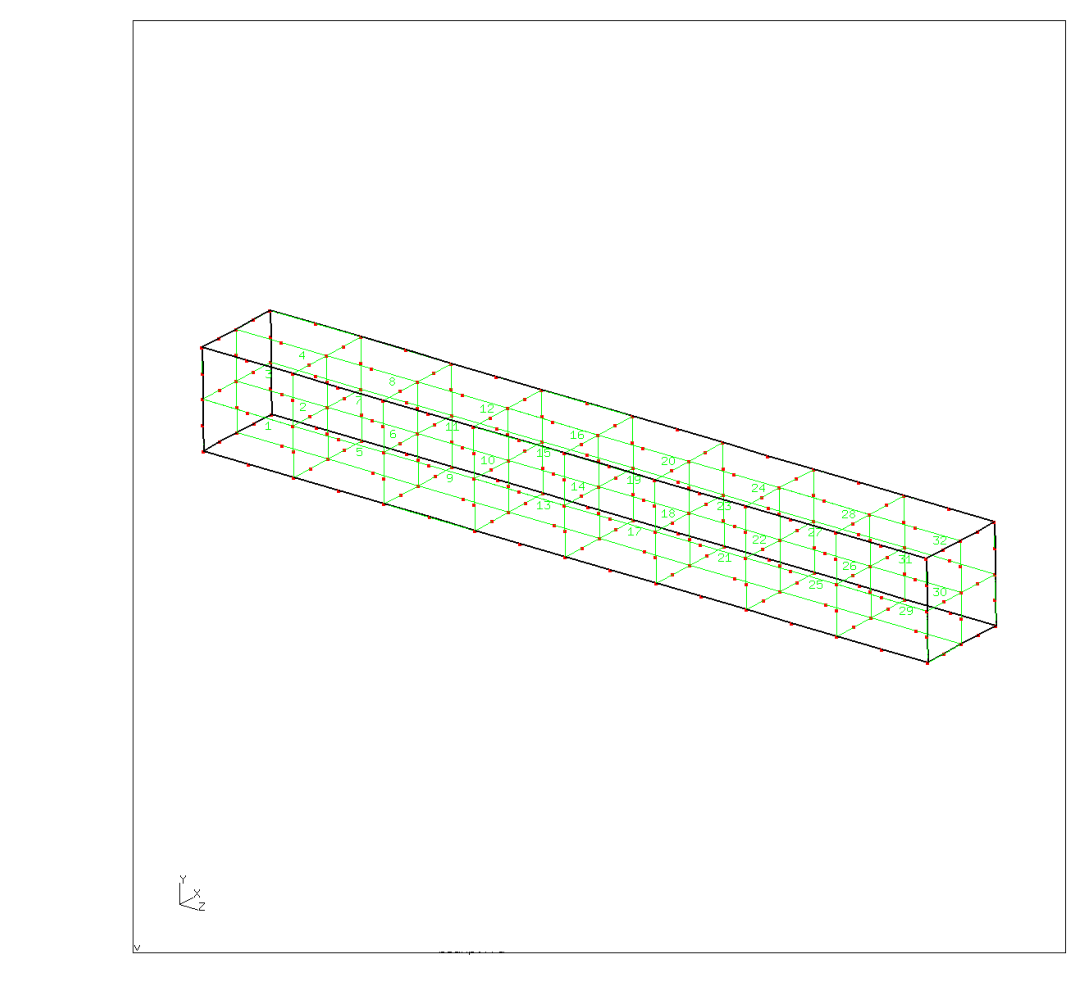
\epsfig{file=Beam2.eps,width=10cm}
\caption{\label{beam2}Mesh for the beam}
\end{figure}

In this section, a cantilever beam loaded by point forces at its free end is
analyzed. 

The geometry, loading and boundary conditions of the cantilever beam are shown in Figure
\ref{beam1}. The size of the beam is 1x1x8 $m^3$, the loading consists of a
point force of $9 \times 10^6$ N and the beam is completely fixed (in all directions) on the left end. Let us take 1 m and 1 MN as units of length and force, respectively. Assume that the beam geometry was generated and meshed with CalculiX GraphiX (cgx) resulting in the mesh in Figure \ref{beam2}. For reasons of clarity, only element labels are displayed.

A CalculiX input deck basically consists of a model definition section describing the geometry and boundary conditions of the problem and one or more steps (Figure \ref{beam3}) defining the loads.

\begin{figure}
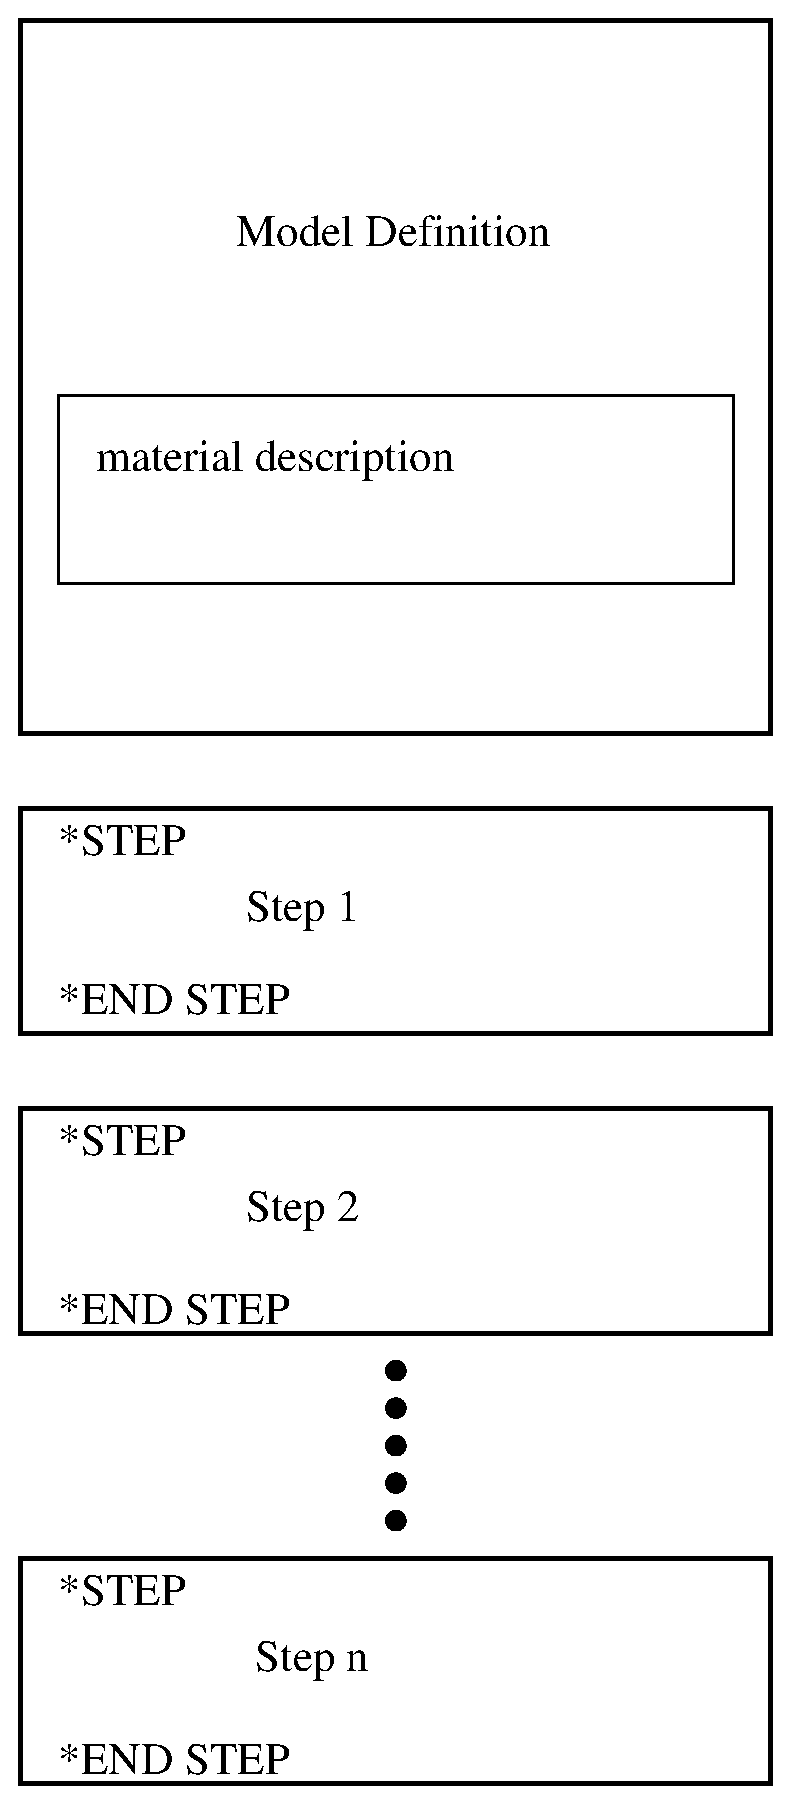
\epsfig{file=Beam3.eps,width=8cm}
\caption{\label{beam3}Structure of a CalculiX input deck}
\end{figure}

The model definition section starts at the beginning of the file and ends at the occurrence of the first *STEP card. All input is preceded by keyword cards, which all start with an asterisk (*), indicating the kind of data which follows. *STEP is such a keyword card. Most keyword cards are either model definition cards (i.e. they can only occur before the first *STEP card) or step cards (i.e. they can only occur between *STEP and *END STEP cards). A few can be both.

In our example (Figure \ref{beam4}), the first keyword card is *HEADING, followed by a short description of the problem. This has no effect on the output and only serves for identification. Then, the coordinates are given as triplets preceded by the *NODE keyword. Notice that data on the same line are separated by commas and must not exceed a record length of 132 columns. A keyword card can be repeated as often as needed. For instance, each node could have been preceded by its own *NODE keyword card.

\begin{figure}
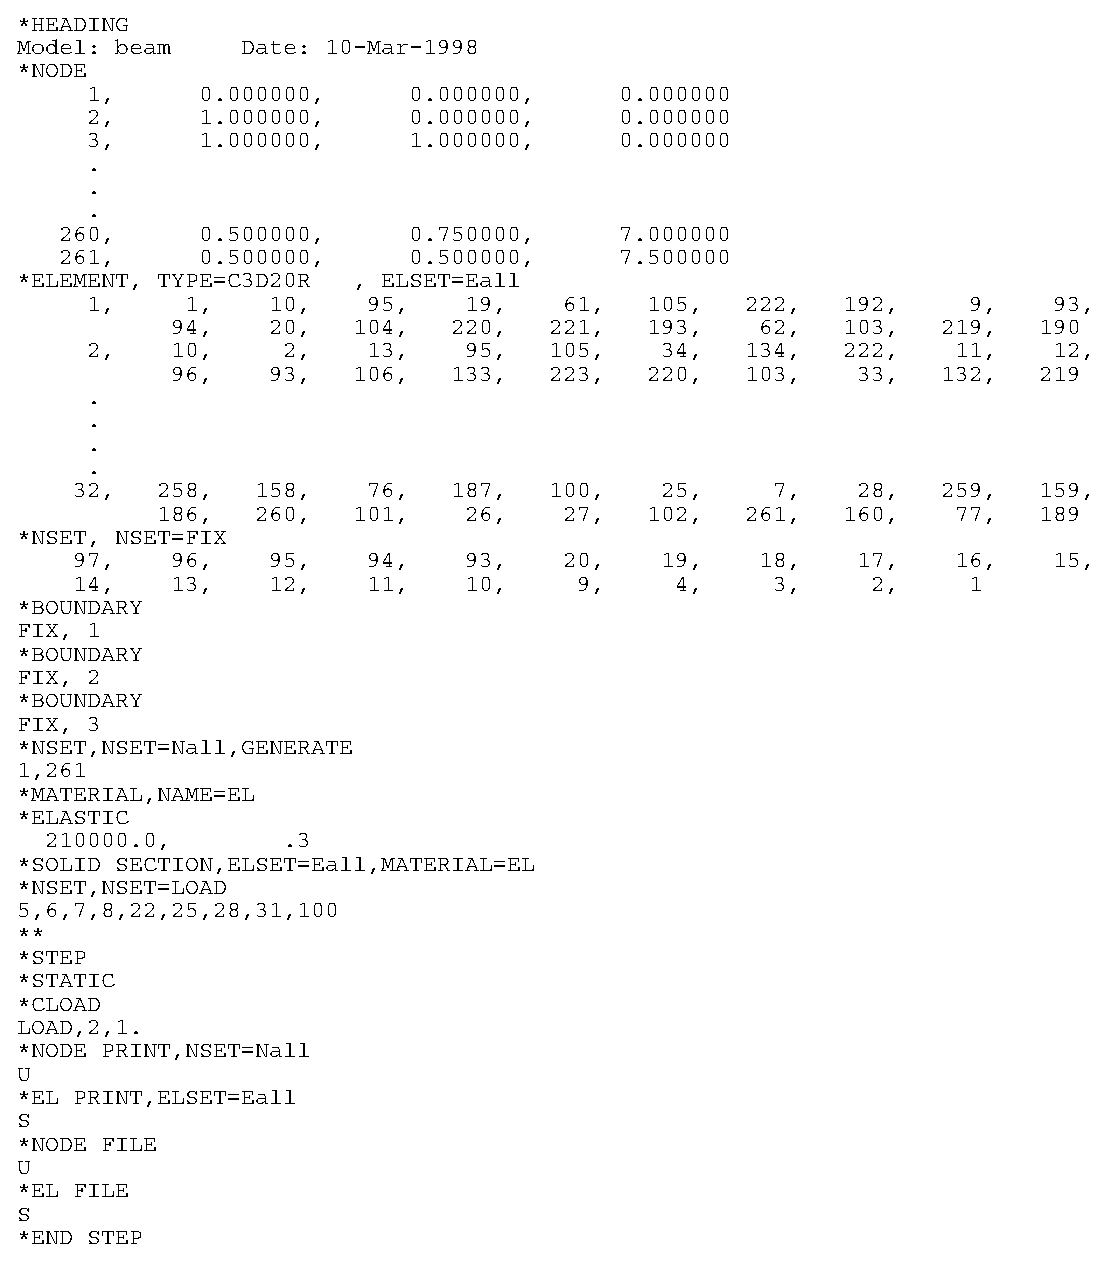
\epsfig{file=BeamInputDeck.eps,width=12cm}
\caption{\label{beam4}Beam input deck}
\end{figure}

\begin{figure}
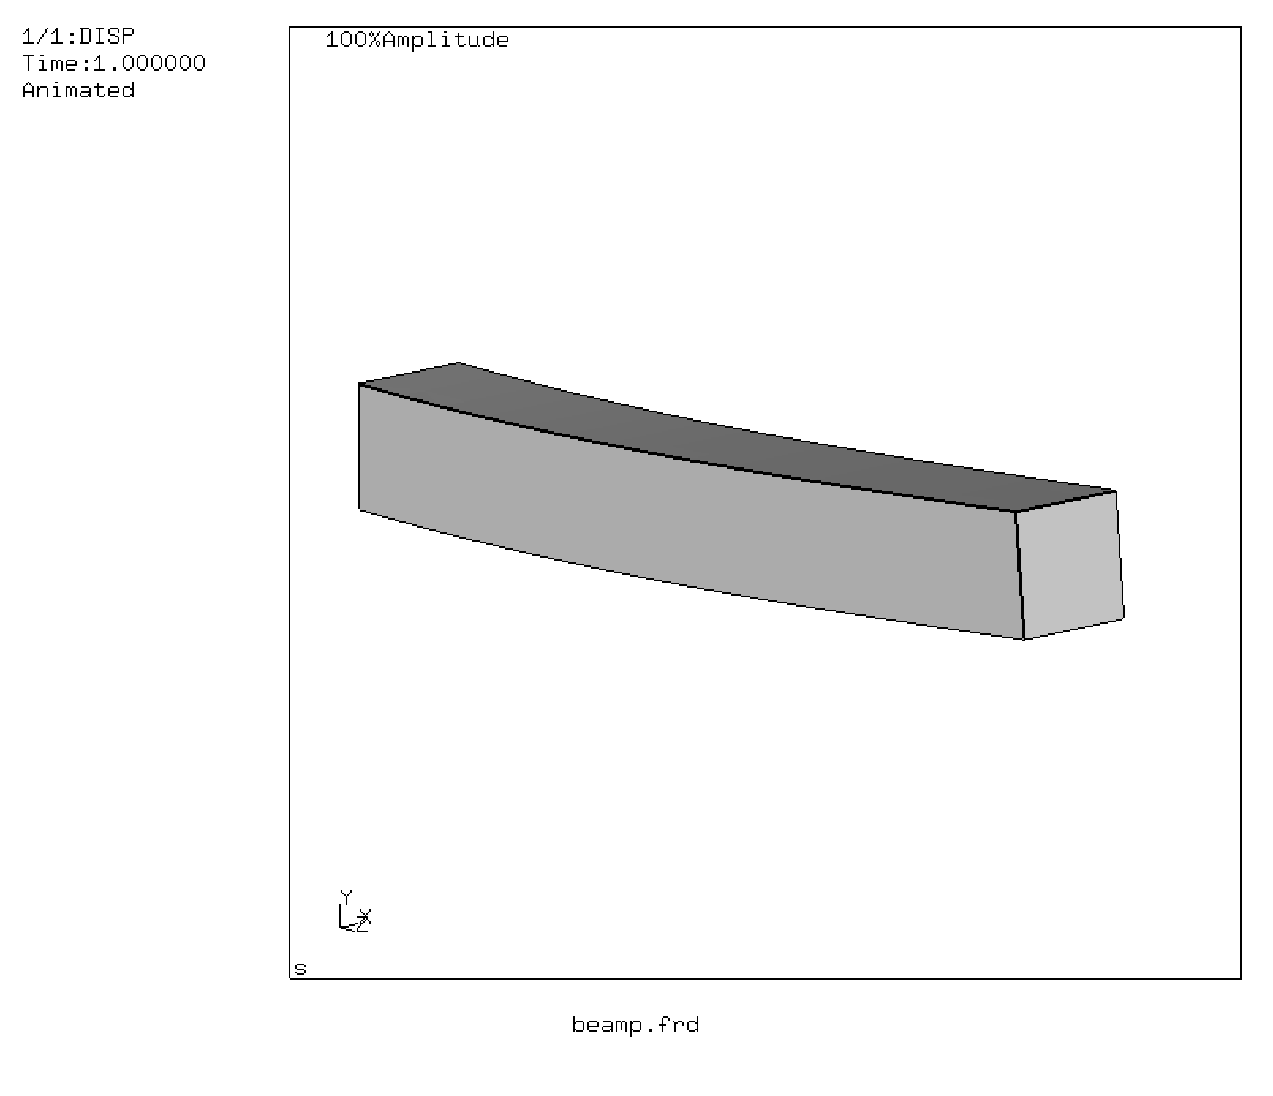
\epsfig{file=Beam5.eps,width=9cm}
\caption{\label{beam5}Deformation of the beam}
\end{figure}

Next, the topology is defined by use of the keyword card *ELEMENT. Defining the topology means listing for each element its type, which nodes belong to the element and in what order. The element type is a parameter on the keyword card. In the beam case 20-node brick elements with reduced integration have been used, abbreviated as C3D20R. In addition, by adding ELSET=Eall, all elements following the *ELEMENT card are stored in set Eall. This set will be later referred to in the material definition. Now, each element is listed followed by the 20 node numbers defining it. With *NODE and *ELEMENT, the core of the geometry description is finished. Remaining model definition items are geometric boundary conditions and the material description.

The only geometric boundary condition in the beam problem is the fixation at z=0. To this end, the nodes at z=0 are collected and stored in node set FIX defined by the keyword card *NSET. The nodes belonging to the set follow on the lines underneath the keyword card. By means of the card *BOUNDARY, the nodes belonging to set FIX are subsequently fixed in 1, 2 and 3-direction, corresponding to x,y and z. The three *BOUNDARY statements in Figure \ref{beam4} can actually be grouped yielding:

\begin{verbatim}
*BOUNDARY
FIX,1
FIX,2
FIX,3
\end{verbatim}

or even shorter:

\begin{verbatim}
*BOUNDARY
FIX,1,3
\end{verbatim}

meaning that degrees of freedom 1 through 3 are to be fixed (i.e. set to zero).

The next section in the input deck is the material description. This section is special since the cards describing one and the same material must be grouped together, although the section itself can occur anywhere before the first *STEP card. A material section is always started by a *MATERIAL card defining the name of the material by means of the parameter NAME. Depending on the kind of material several keyword cards can follow. Here, the material is linear elastic, characterized by a Young's modulus of 210,000.0 $MN/{m^2}$ and a Poisson coefficient of 0.3 (steel). These properties are stored beneath the *ELASTIC keyword card, which here concludes the material definition. Next, the material is assigned to the element set Eall by means of the keyword card *SOLID SECTION.

Finally, the last card in the model definition section defines a node set LOAD which will be needed to define the load. The card starting with two asterisks in between the model definition section and the first step section is a comment line. A comment line can be introduced at any place. It is completely ignored by CalculiX and serves for input deck clarity only.

\begin{figure}
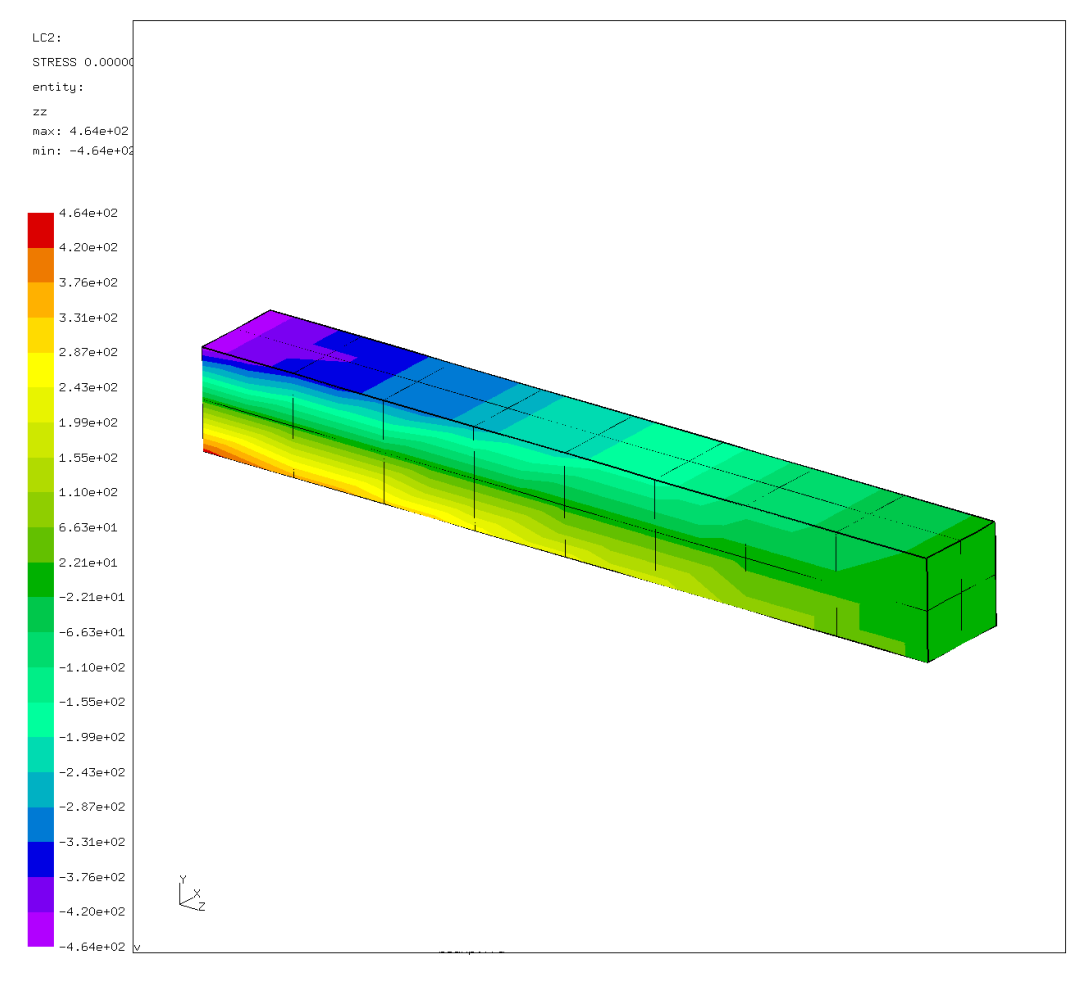
\epsfig{file=Beam6.eps,width=9cm}
\caption{\label{beam6}Axial normal stresses in the beam}
\end{figure}

In the present problem, only one step is needed. A step always starts with a
*STEP card and concludes with a *END STEP card. The keyword card *STATIC
defines the procedure. The *STATIC card indicates that the load is applied in
a quasi-static way, i.e. so slow that mass inertia does not play a role. Other
procedures are *FREQUENCY, *BUCKLE, *MODAL DYNAMIC, *STEADY STATE DYNAMICS and
*DYNAMIC. Next, the concentrated load is applied (keyword *CLOAD) to node set LOAD. The forces act in y-direction and their magnitude is 1, yielding a total load of 9.

Finally, the printing and file storage cards allow for user-directed output generation. The print cards (*NODE PRINT and *EL PRINT) lead to an ASCII file with extension .dat. If they are not selected, no .dat file is generated. The *NODE PRINT and *EL PRINT cards must be followed by the node and element sets for which output is required, respectively. Element information is stored at the integration points. 

The *NODE FILE and *EL FILE cards, on the other hand, govern the output written to an ASCII file with extension .frd. The results in this file can be viewed with CalculiX GraphiX (cgx). Quantities selected by the *NODE FILE and *EL FILE cards are always stored for the complete model. Element quantities are extrapolated to the nodes, and all contributions in the same node are averaged. Selection of fields for the *NODE PRINT, *EL PRINT, *NODE FILE and *EL FILE cards is made by character codes: for instance, U are the displacements and S are the (Cauchy) stresses. 

The input deck is concluded with an *END STEP card. 

The output files for the beam problem consist of file beam.dat and beam.frd. The beam.dat file contains the displacements for set Nall and the stresses in the integration points for set Eall. The file beam.frd contains the displacements and extrapolated stresses in all nodes. It is the input for the visualization program CalculiX GraphiX (cgx). An impression of the capabilities of cgx can be obtained by looking at Figures \ref{beam5}, \ref{beam6} and \ref{beam7}. 

Figure \ref{beam5} shows the deformation of the beam under the prevailing loads. As expected, the beam bends due to the lateral force at its end. Figure \ref{beam6} shows the normal stress in axial direction. Due to the bending moment one obtains a nearly linear distribution across the height of the beam. Finally, Figure \ref{beam7} shows the Von Mises stress in the beam.

\begin{figure}
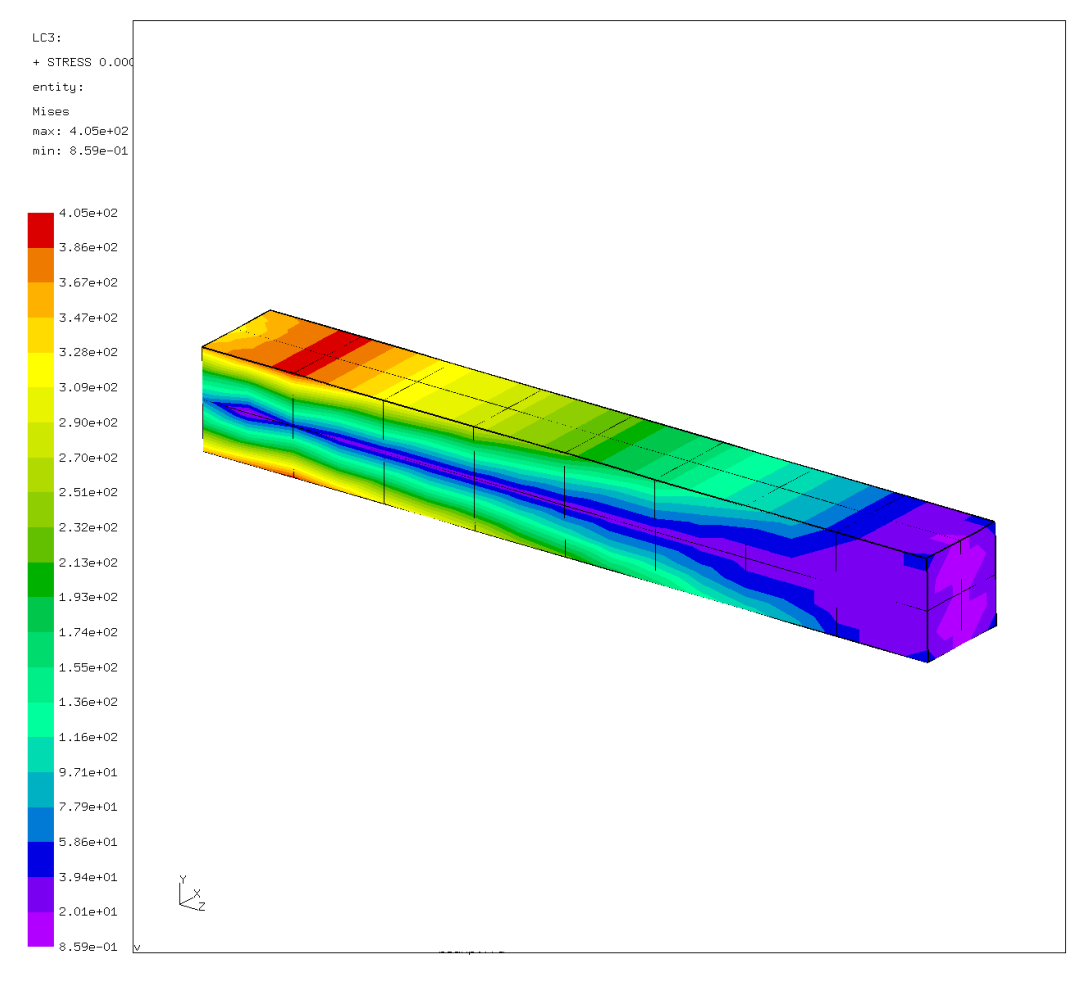
\epsfig{file=Beam7.eps,width=9cm}
\caption{\label{beam7}Von Mises stresses in the beam}
\end{figure}

\subsection{Frequency calculation of a beam loaded by compressive forces}

Let us consider the beam from the previous section and determine its
eigenfrequencies and eigenmodes. To obtain different frequencies for the
lateral directions the cross section is changed from 1x1 to 1x1.5. Its length
is kept (8 length units). The input deck is very similar to the one in the
previous section (the full deck is part of the
test example suite: beamf2.inp): 

\begin{verbatim}
**
**   Structure: beam under compressive forces.
**   Test objective: Frequency analysis; the forces are that 
**                   high that the lowest frequency is nearly 
**                   zero, i.e. the buckling load is reached.
**
*HEADING
Model: beam     Date: 10-Mar-1998
*NODE
     1,      0.000000,      0.000000,      0.000000
     ...
*ELEMENT, TYPE=C3D20R
     1,     1,    10,    95,    19,    61,   105,   222,   192,     9,    93,
           94,    20,   104,   220,   221,   193,    62,   103,   219,   190
           ...
*BOUNDARY
CN7, 1
*BOUNDARY
CN7, 2
*BOUNDARY
CN7, 3
*ELSET,ELSET=EALL,GENERATE
1,32
*MATERIAL,NAME=EL
*ELASTIC
  210000.0,        .3
*DENSITY
7.8E-9
*SOLID SECTION,MATERIAL=EL,ELSET=EALL
*NSET,NSET=LAST
     5,  
     6,  
     ...
*STEP
*STATIC
*CLOAD
LAST,3,-48.155
*END STEP
*STEP,PERTURBATION
*FREQUENCY
10
*NODE FILE
U
*EL FILE
S
*END STEP
     
\end{verbatim}

The only significant differences relate to the steps. In the first step the
preload is applied in the form of compressive forces at the end of the
beam. In each node belonging to set LAST a compressive force is applied with
a value of -48.155 in the positive z-direction, or, which is equivalent, with
magnitude 48.155 in the negative z-direction. The second step is a frequency
step. By using the parameter PERTURBATION on the *STEP keyword card the user
specifies that the deformation and stress from the previous static step
should be taken into account in the subsequent frequency calculation. The
*FREQUENCY card and the line underneath indicate that this is a modal analysis
step and that the 10 lowest eigenfrequencies are to be determined. They are
automatically stored in the .dat file. Table
\ref{tabfreq} shows these eigenfrequencies for the beam without and with
preload together with a comparison with ABAQUS (the input deck for the modal
analysis without preload is stored in file beamf.inp of the test example suite). One notices that due to the
preload the eigenfrequencies drop. This is especially outspoken for the
lower frequencies. As a matter of fact, the lowest bending eigenfrequency is
so low that buckling will occur. Indeed, one way of determining the buckling
load is by increasing the compressive load up to the point that the lowest
eigenfrequency is zero. For the present example this means that the buckling
load is 21 x 48.155 = 1011.3 force units (the factor 21 stems from the fact
that the same load is applied in 21 nodes). An alternative way of determining
the buckling load is to use the \htmlref{*BUCKLE}{buckle} keyword card. This
is illustrated for the same beam geometry in file beamb.inp of the test suite.

\begin{table}
\caption{Frequencies without and with preload (cycles/s).\label{tabfreq}}
\begin{center}
\begin{tabular}{|c|c|c|c|}
\hline
\multicolumn{2}{|c|}{without preload} & \multicolumn{2}{c|}{with preload} \\
\hline
CalculiX & ABAQUS & CalculiX & ABAQUS \\
\hline
13,096. & 13,096. & 705. & 1,780. \\
19,320. & 19,319. & 14,614. & 14,822. \\
76,840. & 76,834. & 69,731. & 70,411. \\
86,955. & 86,954. & 86,544. & 86,870. \\
105,964. & 105,956. & 101,291. & 102,148. \\
162,999. & 162,998. & 162,209. & 163,668. \\
197,645. & 197,540. & 191,581. & 193,065. \\
256,161. & 256,029. & 251,858. & 253,603. \\
261,140. & 261,086. & 259,905. & 260,837. \\
351,862. & 351,197. & 345,729. & 347,688. \\
\hline
\end{tabular}
\end{center}        
\end{table}

Figures \ref{beam8} and \ref{beam9} show the deformation of the second bending mode across the
minor axis of inertia and deformation of the first torsion mode.

\begin{figure}
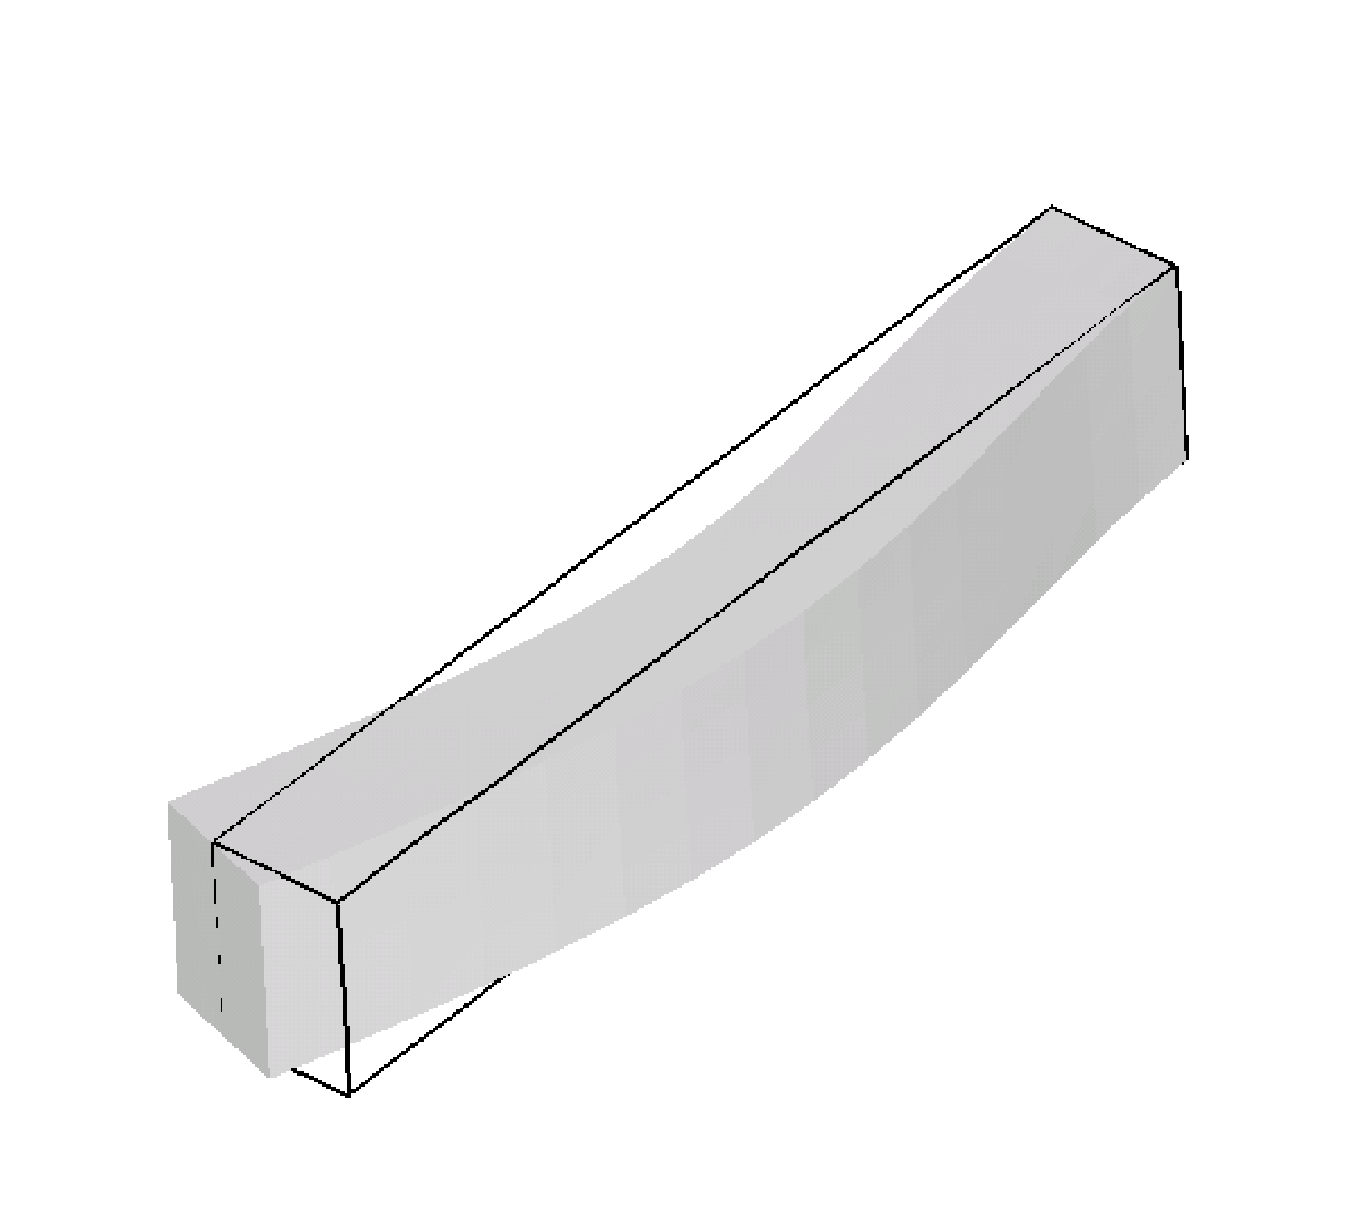
\epsfig{file=Beam8.eps,width=9cm}
\caption{\label{beam8}Second bending mode across the minor axis of inertia}
\end{figure}

\begin{figure}
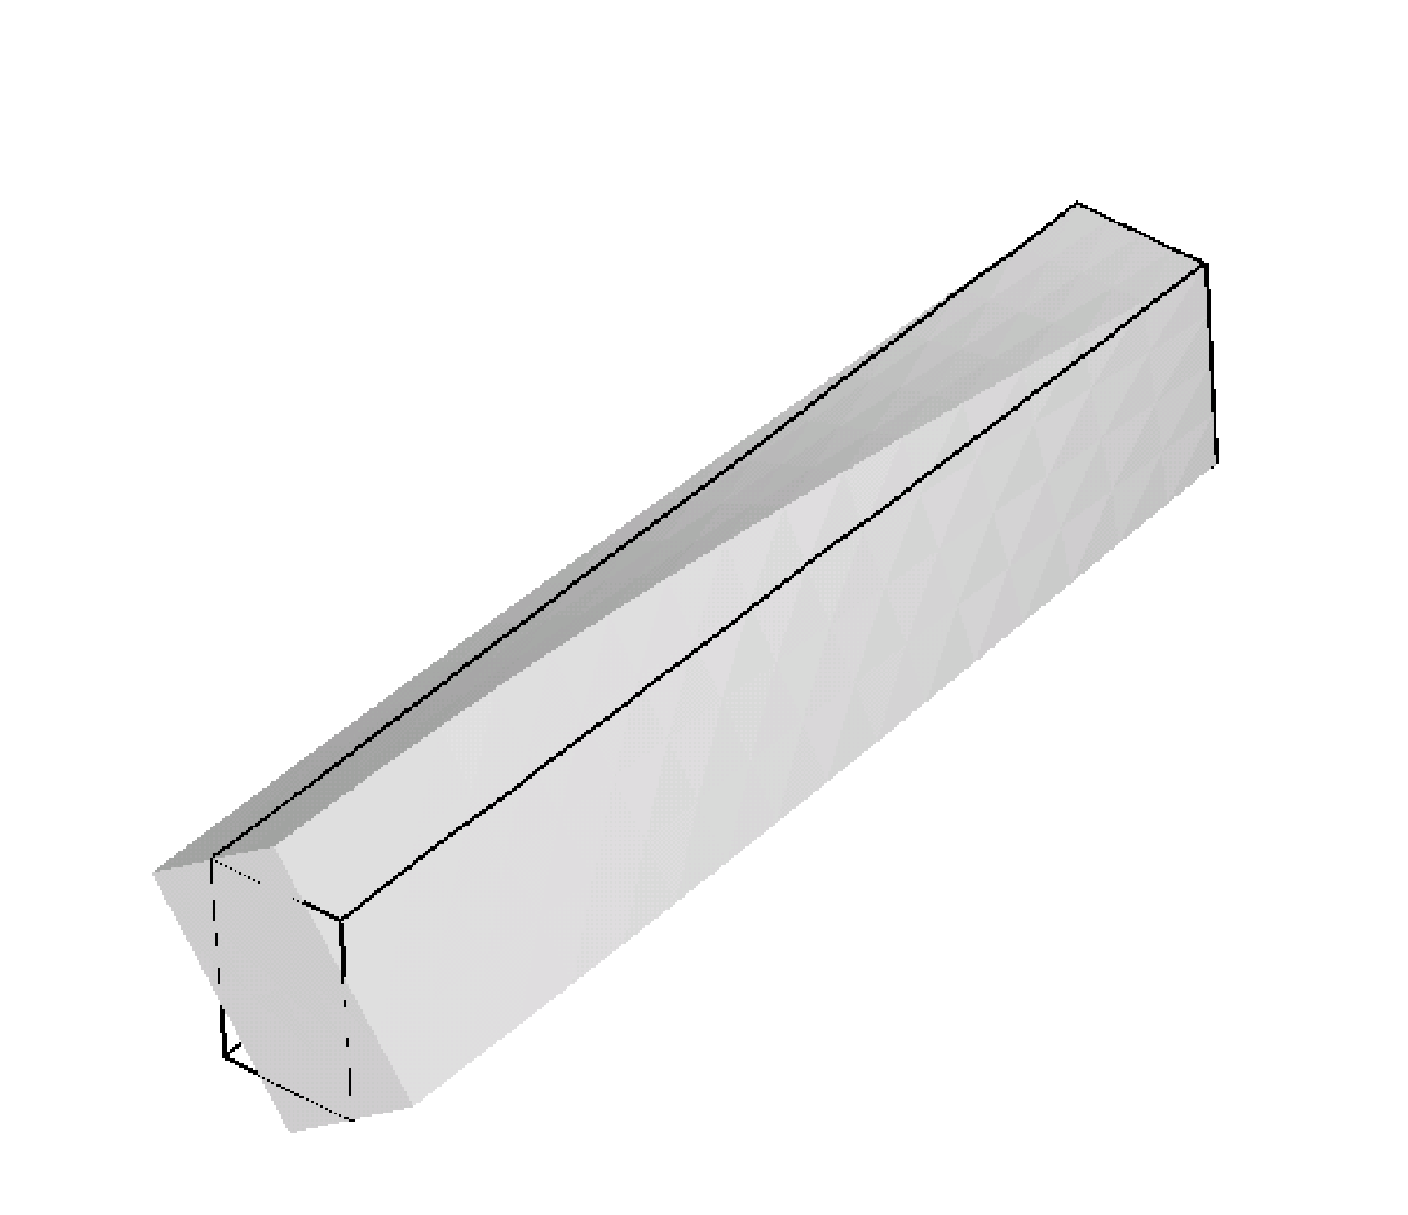
\epsfig{file=Beam9.eps,width=9cm}
\caption{\label{beam9}First torsion mode}
\end{figure}

\subsection{Frequency calculation of a rotating disk on a slender shaft}

\begin{verbatim}
**
**   Structure: slender disk mounted on a long axis
**   Test objective: *COMPLEX FREQUENCY,
**                   output of moments of inertia.
**
*NODE, NSET=Nall
       1,6.123233995737e-17,1.000000000000e+00,0.000000000000e+00
       ...
*ELEMENT, TYPE=C3D20R, ELSET=Eall
     1,     1,     2,     3,     4,     5,     6,     7,     8,     9,    10,
          11,    12,    17,    18,    19,    20,    13,    14,    15,    16
          ...
*BOUNDARY
Nfix,1,3
*Solid Section, elset=Eall, material=steel
*Material, name=STEEL
*Elastic
 210000., 0.3
*DENSITY
7.8e-9
*Step,nlgeom
*Static
*dload
Eall,centrif,3.0853e8,0.,0.,0.,0.,0.,1. 
*end step
*step,perturbation
*frequency,STORAGE=YES
 10,
*end step
*step,perturbation
*complex frequency,coriolis
10,
*node file
pu
*end step
\end{verbatim}
          
\begin{figure}
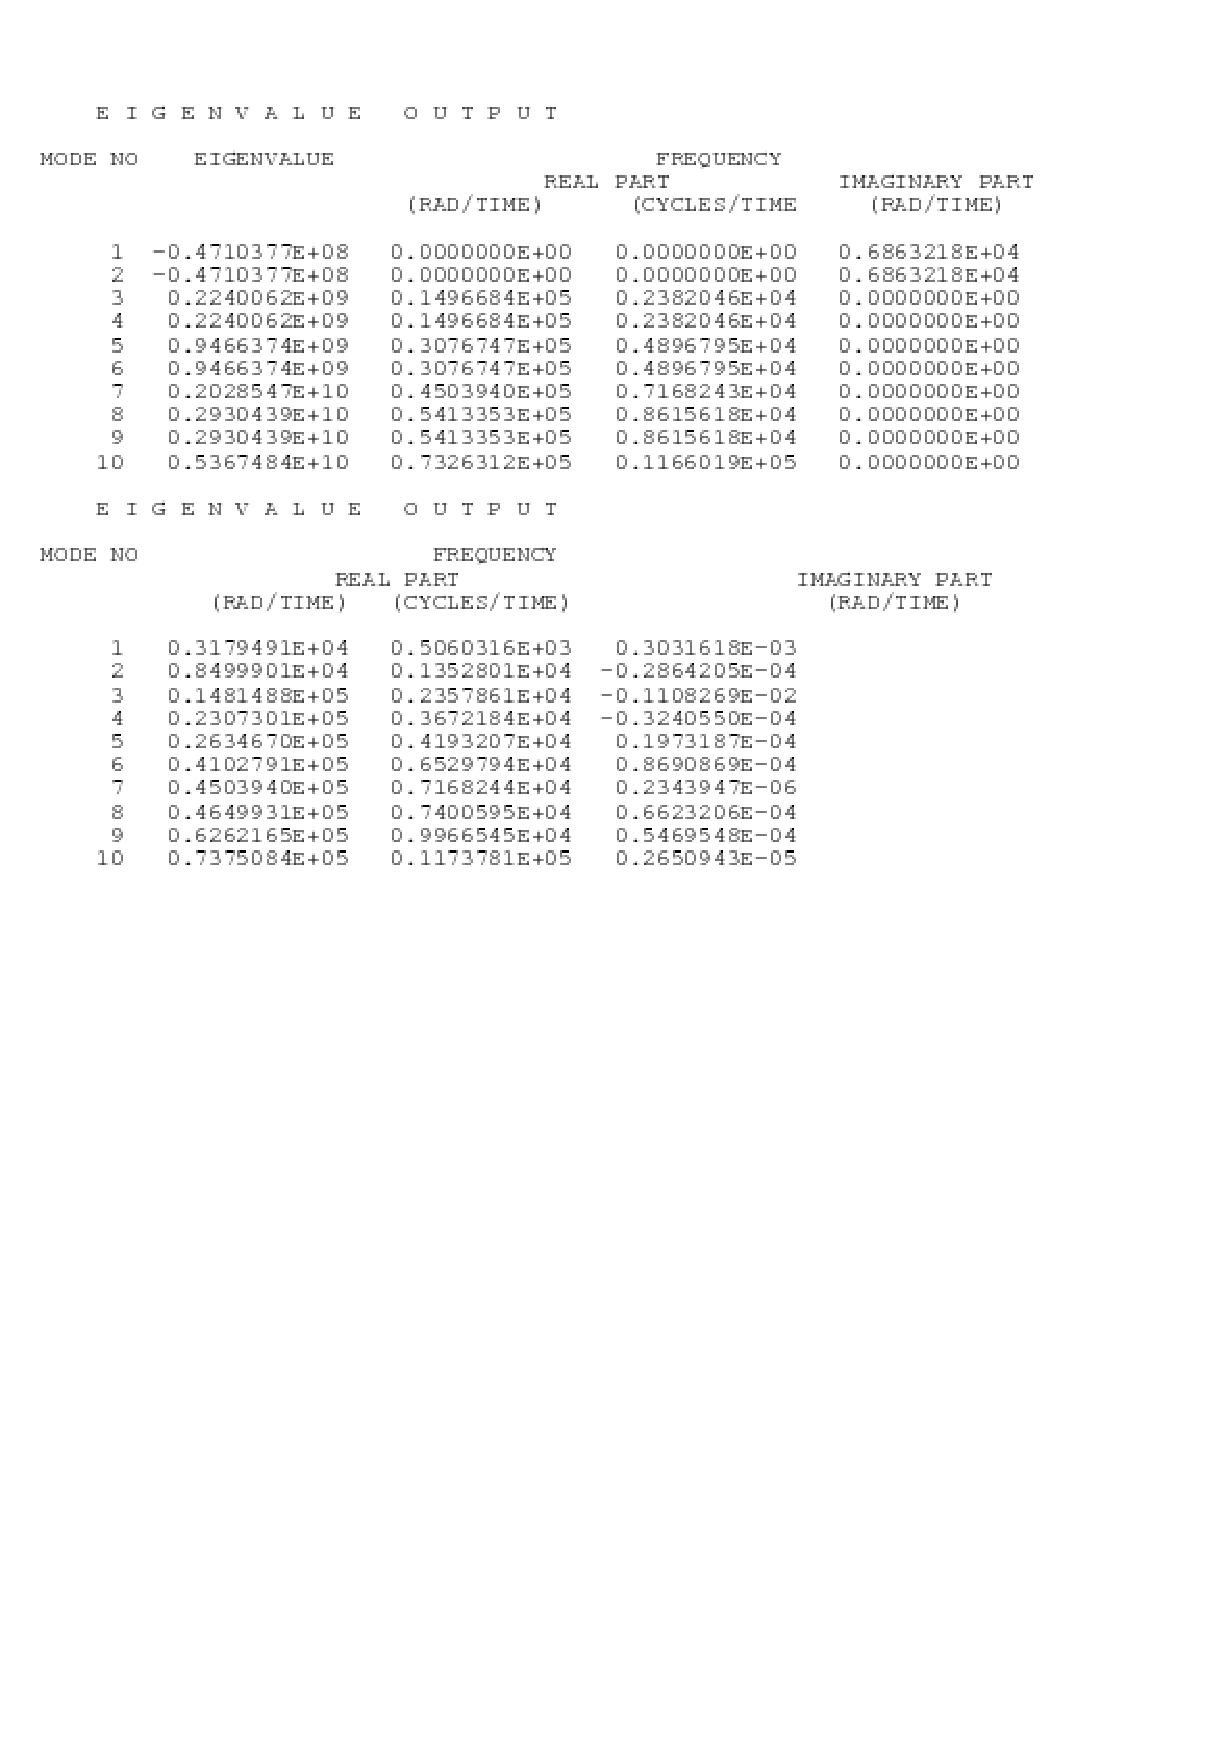
\epsfig{file=rotor4.eps,width=12cm}
\caption{\label{rotor4}Eigenfrequencies for the rotor}
\end{figure}

This is an example for a complex frequency calculation. A disk with an outer
diameter of 10, an inner diameter of 2 and a thickness of 0.25 is mounted on a hollow shaft with
outer diamter 2 and inner diameter 1 (example rotor.inp in het test
examples). The disk is mounted in het middle of the shaft, the ends of which
are fixed in all directions. The length of the shaft on either side of the
disk is 50. The input deck for this example is shown above. 

The deck start with the definition of the nodes and elements. The set Nfix
contains the nodes at the end of the shaft, which are fixed in all
directions. The material is ordinary steel. Notice that the density is needed
for the centrifugal loading.

Since the disk is rotation there is a preload in the form of centrifugal
forces. Therefore, the first step is a nonlinear geometric static step in
order to calculate the deformation and stresses due to this loading. By
selecting the parameter perturbation in the subsequent frequency step this
preload is taken into account in the calculation of the stiffness matrix in
the frequency calculation. The resulting eigenfrequencies are stored at the
top of file
rotor.dat (Figure \ref{rotor4} for a rotational speed of 9000 rad/s). In a
*FREQUENCY step an eigenvalue problem is solved, the eigenvalues of which
(first column on the top of Figure \ref{rotor4}) are
the square of the eigenfrequencies of the structure (second to fourth
column). If the eigenvalue is negative, an imaginary eigenfrequency
results. This is the case for the two lowest eigenvalues for the rotor
rotating at 9000 rad/s. For shaft speeds underneath about 6000 rad/s all
eigenfrequencies are real. The lowest eigenfrequencies as a function of
rotating speeds up to 18000 rad/s are shown in  Figure \ref{rotor5} (+ and x
curves). 

\begin{figure}
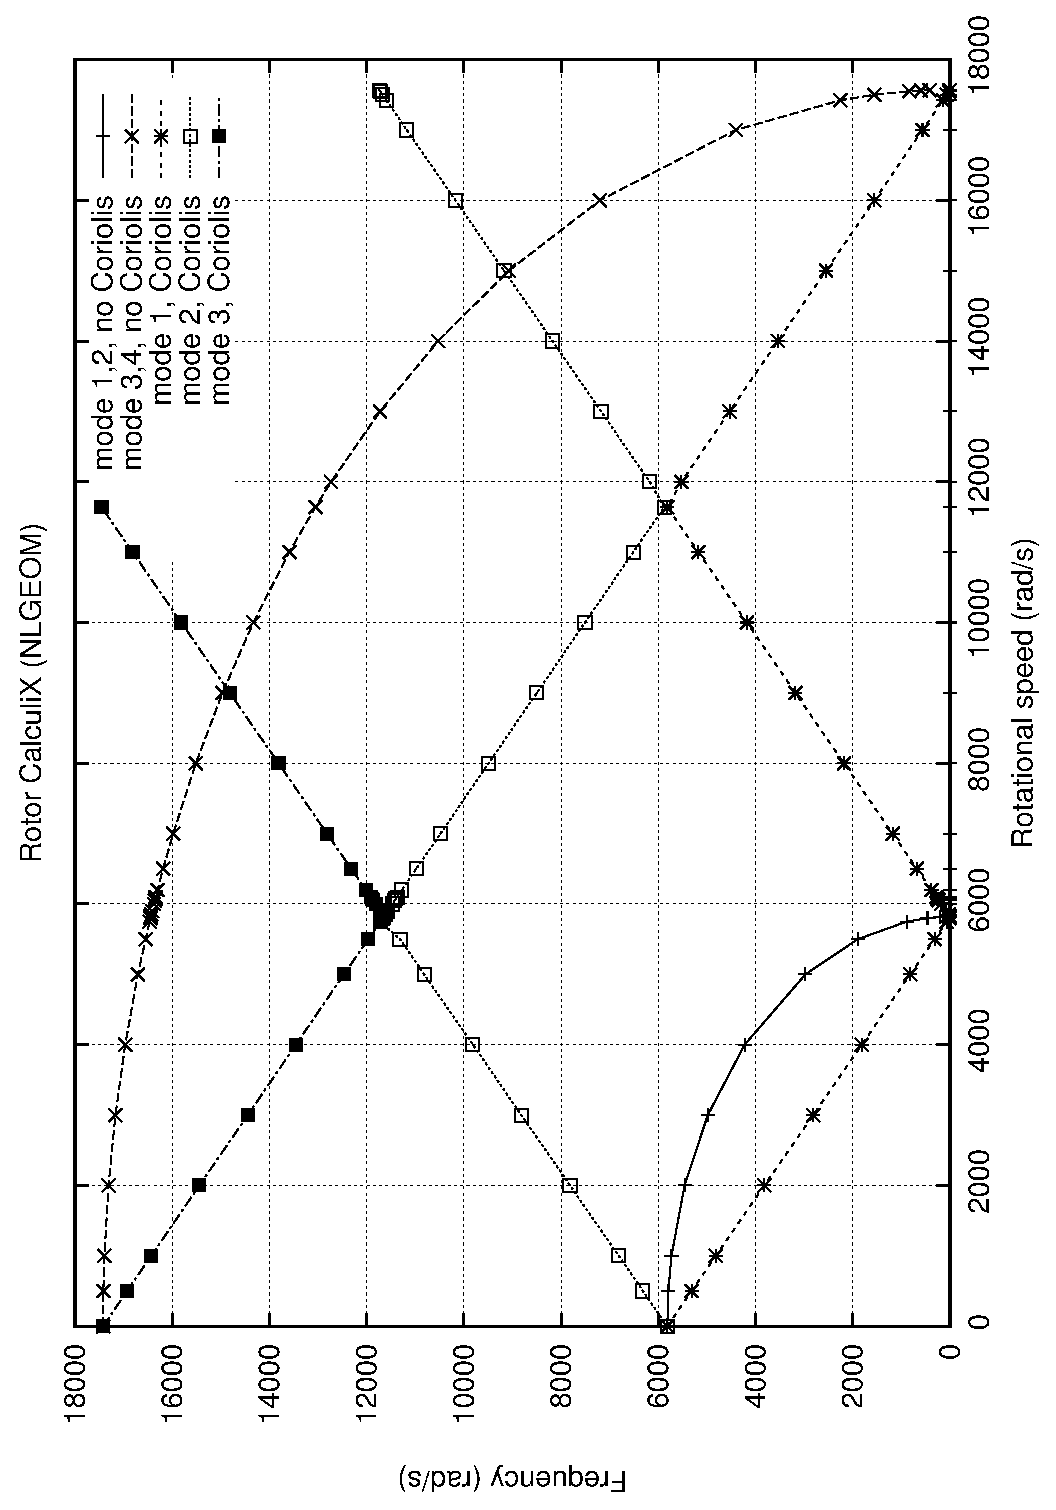
\epsfig{file=rotor5.eps,width=8cm,angle=270}
\caption{\label{rotor5}Eigenfrequencies as a function of shaft speed}
\end{figure}

What is the physical meaning of imaginary eigenfrequencies? The eigenmodes
resulting from a frequency calculation contain the term $e^{i \omega t}$. If
the eigenfrequency $\omega$ is real, one obtains a sine or cosine, if $\omega$
is imaginary, one obtains an increasing or decreasing exponential
function \cite{Dhondt}. Thus, for imaginary eigenfrequencies the response is not any more
oscillatory: it increases indefinitely, the system breaks apart. Looking at
Figure \ref{rotor5} one observes that the lowest eigenfrequency decreases for
increasing shaft speed up to the point where it is about zero at a shaft speed
of nearly 6000 rad/s. At that point the eigenfrequency becomes imaginary, the rotor
breaks apart. This has puzzled engineers for a long time, since real systems
were observed to reach supercritical speeds without breaking apart.

The essential point here is to observe that the calculations are being
performed in a rotating coordinate system (fixed to the shaft). Newton's laws
are not valid in an accelerating reference system, and a rotating coordinate
system is accelerating. A correction term to Newton's laws is necessary in the
form of a Coriolis force. The introduction of the Coriolis force leads to a
complex nonlinear eigenvalue system, which can solved with the
\htmlref{*COMPLEX FREQUENCY}{complexfrequency} procedure (cf. Section
\ref{complexfrequencyanalysis}). One can prove that the resulting
eigenfrequencies are real, the eigenmodes, however, are usually complex. This
leads to rotating eigenmodes. 

In order to use the *COMPLEX FREQUENCY procedure the eigenmodes without
Coriolis force must have been calculated and stored in a previous *FREQUENCY
step (STORAGE=YES) (cf. Input Deck). The complex frequency response is calculated as a linear
combination of these eigenmodes. The number of eigenfrequencies requested in
the *COMPLEX FREQUENCY step should not exceed those of the preceding
*FREQUENCY step. Since the eigenmodes are complex, they are best stored in
terms of amplitude and phase with PU underneath the *NODE FILE card.

\begin{figure}
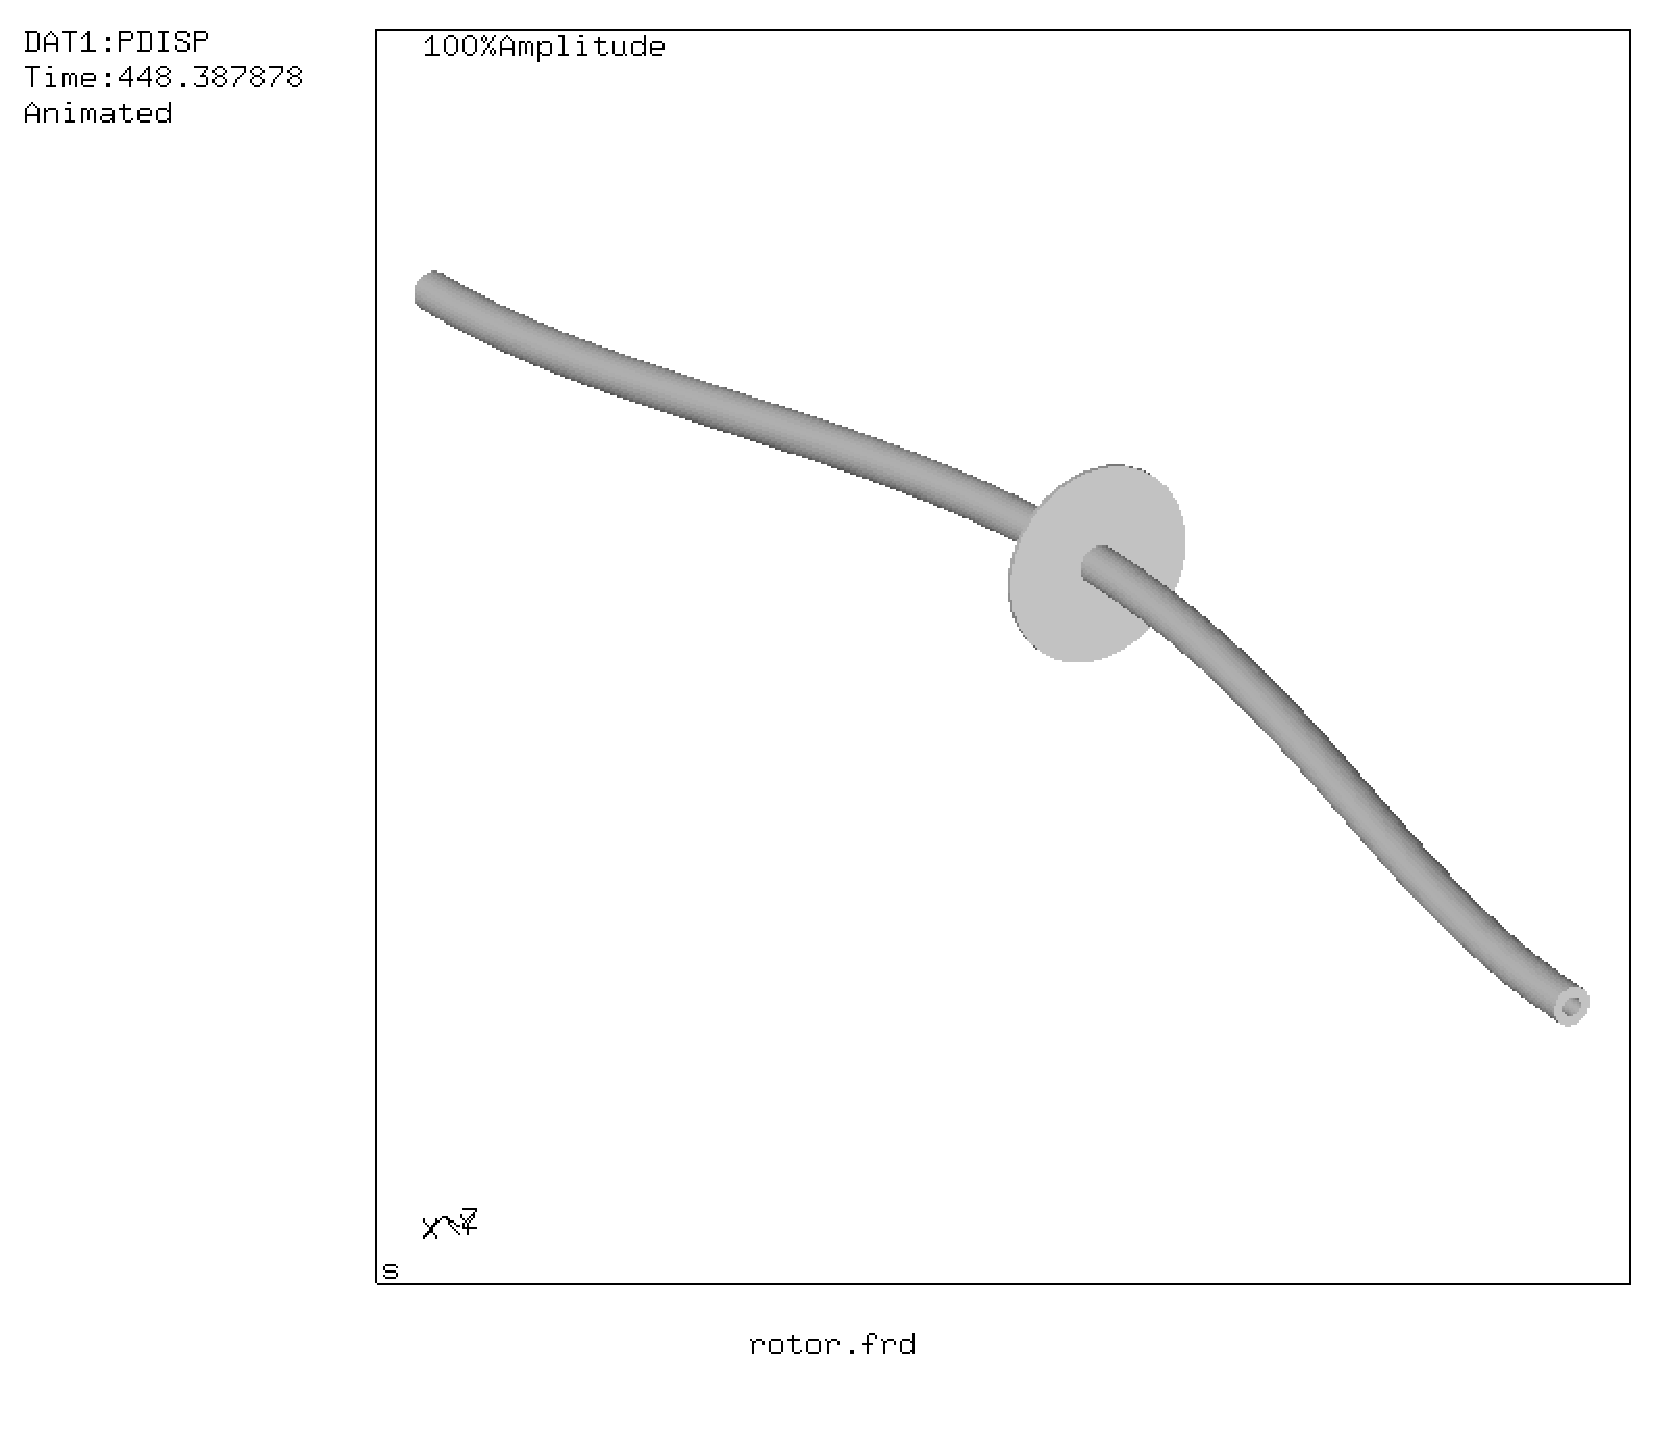
\epsfig{file=rotor2.eps,width=8cm}
\caption{\label{rotor2}Two-node eigenmode}
\end{figure}

\begin{figure}
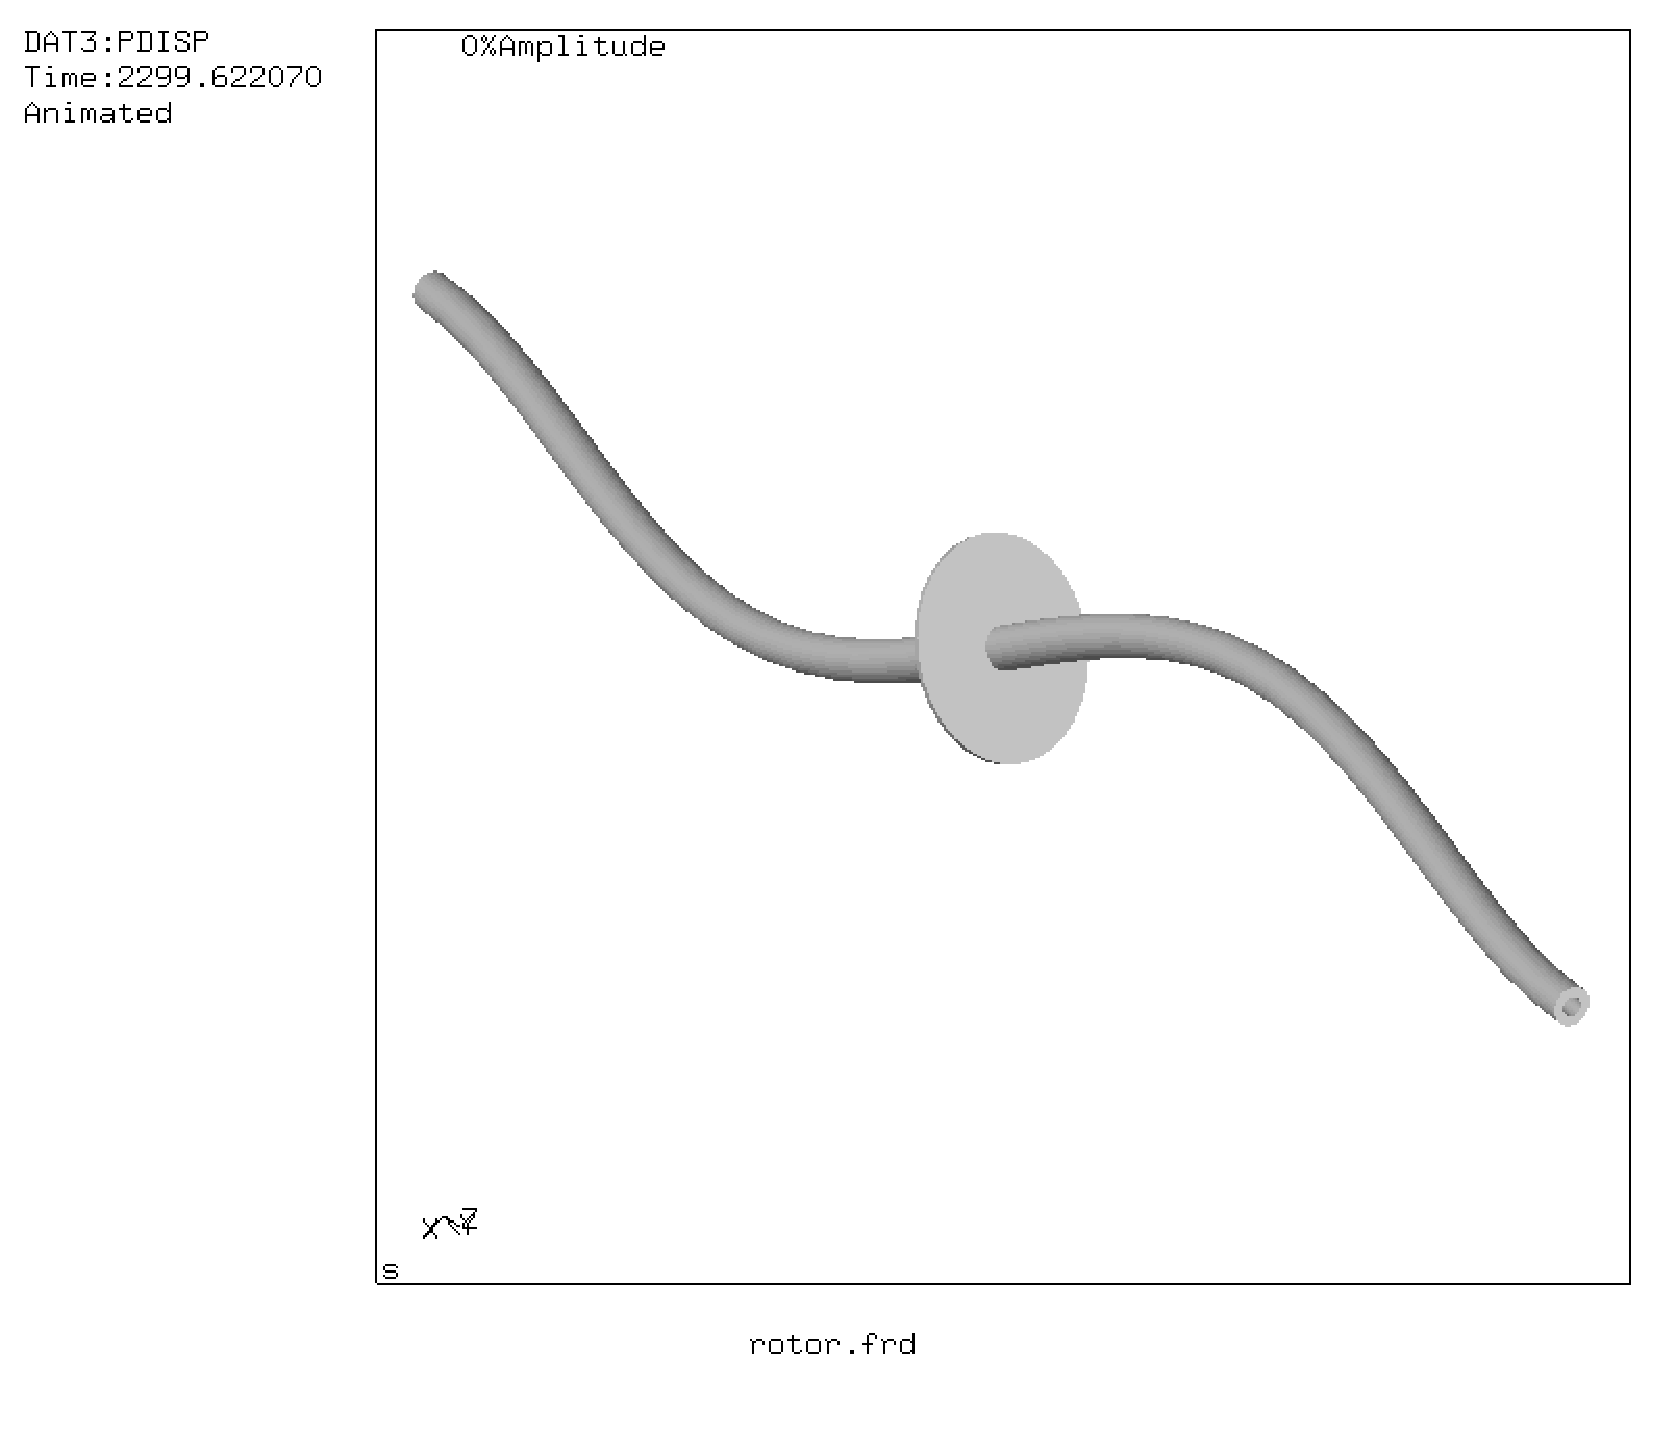
\epsfig{file=rotor3.eps,width=8cm}
\caption{\label{rotor3}Three-node eigenmode}
\end{figure}

The correct eigenvalues for the rotating shaft lead to the straight lines in
Figure \ref{rotor5}. Each line represents an eigenmode: the lowest decreasing
line is a two-node counter clockwise (ccw) eigenmode when looking in
(-z)-direction, the highest decreasing line is a three-node ccw eigenmode, the
lowest and highest increasing lines constitute both a two-node clockwise (cw)
eigenmode. A node is a location at which the radial motion is zero. Figure
\ref{rotor2} shows the two-node eigenmode, Figure \ref{rotor3} the three-node
eigenmode. Notice that if the scales on the x- and y-axis in Figure
\ref{rotor5} were the same the lines would be under $45^\circ$. 

It might surprise that both increasing straight lines correspond to one and
the same eigenmode. For instance, for a shaft speed of 5816 rad/s one and the
same eigenmode occurs at an eigenfrequency of 0 and 11632 rad/s. Remember,
however, that the eigenmodes apply to the fixed coordinate system, i.e. as
observed by a non--rotating observer. To obtain the frequencies for
a rotating observer the frequencies have to be considered relative to a
$45^\circ$ straight line through the origin and bisecting the diagram. This
observer will see one and the same eigenmode at 5816 rad/s and -5816 rad/s, so
cw and ccw.

Finally, the Coriolis effect is not always relevant. Generally, slender
rotating structures (large blades...) will exhibit important frequency shifts
due to Coriolis.

\subsection{Thermal calculation of a furnace}

\begin{figure}
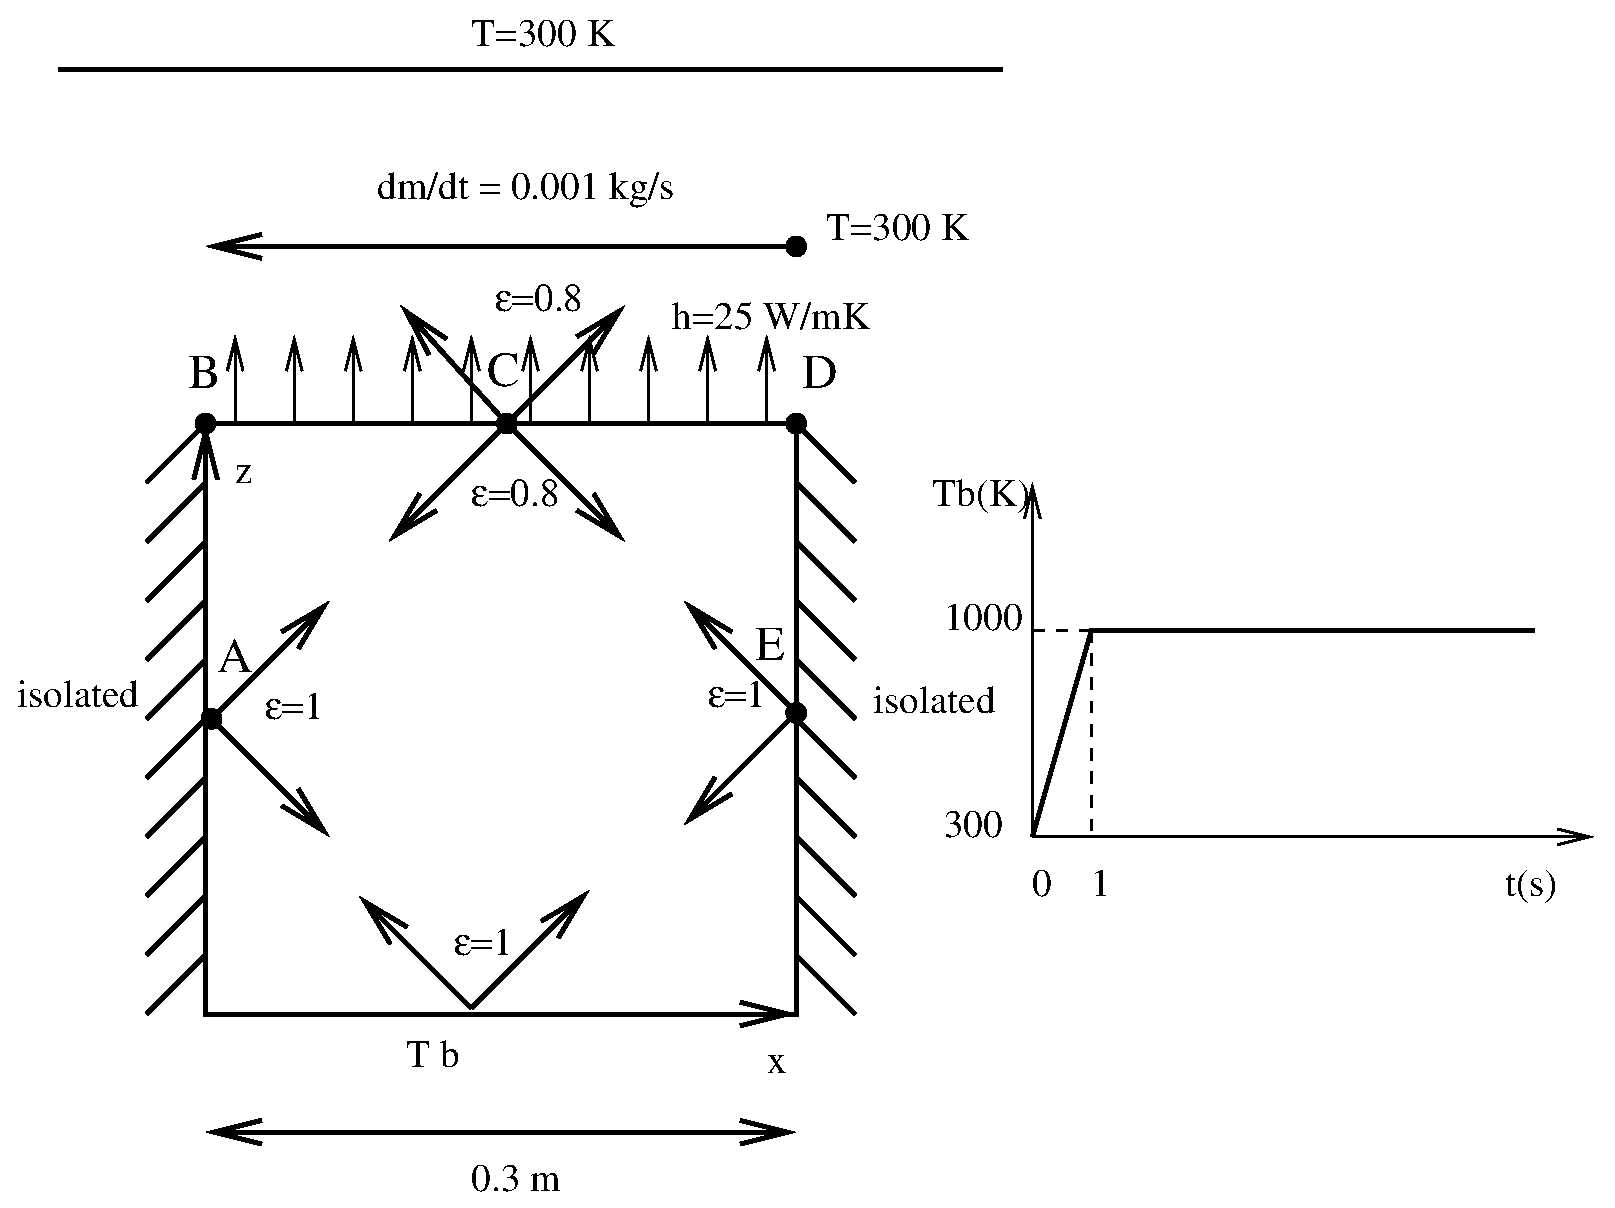
\epsfig{file=furngeo.eps,width=11cm}
\caption{\label{furngeo}Description of the furnace}
\end{figure}

This problem involves a thermal calculation of the furnace depicted in
Figure \ref{furngeo}. The furnace consists of a bottom plate at a temperature
$Tb$, which is prescribed. It changes linearly in an extremely short time from
300 K to 1000 K after which it remains constant. The side walls of the furnace
are isolated from the outer world, but exchange heat through radiation with
the other walls of the furnace. The emissivity of the side walls and bottom
is $\epsilon=1$. The top of the furnace exchanges heat through radiation with
the other walls and with the environmental temperature which is fixed at 300
K. The emissivity of the top is $\epsilon=0.8$. Furthermore, the top exchanges
heat through convection with a fluid (air) moving at the constant rate of
0.001 kg/s. The temperature of the fluid at the right upper corner is 300
K. The walls of the oven are made of 10 cm steel. The material
constants for steels are: heat conductivity $\kappa=50 \mathrm{W/m K}$,
specific 
heat $c=446 \mathrm{W/kg K}$ and density $\rho=7800 \mathrm{kg/m^3}$. The material
constants for 
air are : specific heat $c_p=1000 \mathrm{W/kg K}$ and density $\rho=1
\mathrm{kg/m^3}$. The 
convection coefficient is $h=25 \mathrm{W/m^2 K}$. The dimensions of the furnace
are $0.3 \times 
0.3 \times 0.3 \mathrm{m^3}$ (cube). At $t=0$ all parts are at $T=300
\mathrm{K}$. We would like to know the temperature at locations A,B,C,D and E as a
function of time.  

\begin{verbatim}
**
**   Structure: furnace.
**   Test objective: shell elements with convection and radiation.
**
*NODE, NSET=Nall
       1,  3.00000e-01,  3.72529e-09,  3.72529e-09 
       ...
*ELEMENT, TYPE=S6, ELSET=furnace
     1,      1,      2,      3,      4,      5,      6
     ...
*ELEMENT,TYPE=D,ELSET=EGAS
301,603,609,604
...
*NSET,NSET=NGAS,GENERATE
603,608
*NSET,NSET=Ndown 
1, 
...
*PHYSICAL CONSTANTS,ABSOLUTE ZERO=0.,STEFAN BOLTZMANN=5.669E-8
*MATERIAL,NAME=STEEL
*DENSITY
7800.
*CONDUCTIVITY
50.
*SPECIFIC HEAT
446.
*SHELL SECTION,ELSET=furnace,MATERIAL=STEEL
0.01
*MATERIAL,NAME=GAS
*DENSITY
1.
*SPECIFIC HEAT
1000.
*FLUID SECTION,ELSET=EGAS,MATERIAL=GAS
*INITIAL CONDITIONS,TYPE=TEMPERATURE
Nall,300.
*AMPLITUDE,NAME=A1
0.,.3,1.,1.
*STEP,INC=100
*HEAT TRANSFER
0.1,1.
*VIEWFACTOR,WRITE
*BOUNDARY,AMPLITUDE=A1
Ndown,11,11,1000.
*BOUNDARY
603,11,11,300.
*BOUNDARY,MASS FLOW
609,1,1,0.001
...
*RADIATE
** Radiate based on down
1, R1CR,1000., 1.000000e+00
...
** Radiate based on top
51, R1CR,1000., 8.000000e-01
...
** Radiate based on side
101, R1CR,1000., 1.000000e+00
...
** Radiate based on top
51, R2,300., 8.000000e-01
...
*FILM
51, F2FC, 604, 2.500000e+01
...
*NODE FILE
NT
*NODE PRINT,NSET=NGAS
NT
*END STEP

\end{verbatim}

The input deck is listed above. It starts with the node
definitions. The highest node number in the structure is 602. The nodes 603 up
to 608 are fluid nodes, i.e. in the fluid extra nodes were defined (z=0.3
corresponds with the top of the furnace, z=0 with the bottom). Fluid node 603
corresponds to the location where the fluid temperature is 300 K (``inlet''),
node 608 corresponds to the ``outlet'', the other nodes are located in
between. The coordinates of the fluid nodes actually do not enter the
calculations. Only the convective definitions with the keyword *FILM
govern the exchange between furnace and fluid. With the *ELEMENT card the
6-node shell elements making up the furnace walls are defined. Furthermore,
the fluid nodes are also assigned to elements (element type D), 
so-called network elements. These elements are needed for the assignment of
material properties to the fluid. Indeed, traditionally material properties are
assigned to elements and not to nodes. Each network element consists of two end
nodes, in which the temperature is unknown, and a midside node, which is used
to define the mass flow rate through the element. The fluid nodes 603 up to 613 are
assigned to the network elements 301 up to 305. 

Next, two node sets are defined: GAS contains all fluid nodes, Ndown contains
all nodes on the bottom of the furnace.  

The *PHYSICAL CONSTANTS card is needed in
those analyses in which radiation plays a role. It defines absolute zero, here
0 since we work in Kelvin, and the Stefan Boltzmann constant. In the present
input deck SI units are used throughout. 

Next, the material constants for
STEEL are defined. For thermal analyses the conductivity, specific heat
and density must be defined. The *SHELL SECTION card assigns the STEEL
material to the element set FURNACE, defined by the *ELEMENT statement
before. It contains all elements belonging to the furnace. Furthermore, a
thickness of 0.01 m is assigned. 

The material constants for material GAS consist of the density and the
specific heat. These are the constants for the fluid. Conduction in the fluid
is not considered. The material GAS is assigned to element set EGAS
containing all network elements.

The *INITIAL CONDITIONS card defines an initial temperature of 300 K for all
nodes, i.e. furnace nodes AND fluid nodes. The *AMPLITUDE card defines a ramp
function starting at 0.3 at 0.0 and increasing linearly to 1.0 at 1.0. It will
be used to define the temperature boundary conditions at the bottom of the
furnace. This ends the model definition.

The first step describes the linear increase of the temperature boundary
condition between $t=0$ and $t=1$. The INC=100 parameter on the *STEP card
allows for 100 increments in this step. The procedure is *HEAT TRANSFER,
i.e. we would like to perform a purely thermal analysis: the only unknowns are
the temperature and there are no mechanical unknowns (e.g. displacements). The
step time is 1., the initial increment size is 0.1. Both appear on the line
underneath the *HEAT TRANSFER card. The absence of the parameter STEADY STATE
on the *HEAT TRANSFER card indicates that this is a transient analysis.

Next come the temperature boundary conditions: the bottom plate of the furnace
is kept at 1000 K, but is modulated by amplitude A1. The result is that the
temperature boundary condition starts at 0.3 x 1000 = 300K and increases
linearly to reach 1000 K at t=1 s. The second boundary conditions specifies
that the temperature of (fluid) node 603 is kept at 300 K. This is the inlet
temperature. Notice that ``11'' is the temperature degree of freedom.

The mass flow rate in the fluid is defined with the *BOUNDARY card applied to
the first degree of freedom of the midside nodes of the network elements. The
first line tells us that the mass flow rate in (fluid)node 609 is 0.001. Node
609 is the midside node of network element 301. Since this rate is positive the fluid flows from node
603 towards node 604, i.e. from the first node of network element 301 to the
third node. The user must assure conservation of mass (this is
actually also checked by the program).

The first set of radiation boundary conditions specifies that the top face of
the bottom of the furnace radiates through cavity radiation with an emissivity
of 1 and an environment temperature of 1000 K. For cavity radiation the
environment temperature is used in case the viewfactor at some location does
not amount to 1. What is short of 1 radiates towards the environment. The
first number in each line is the element, the number in the label (the second
entry in each line) is the face of the element exposed to radiation. In
general, these lines are generated automatically in cgx (CalculiX GraphiX).

\begin{figure}
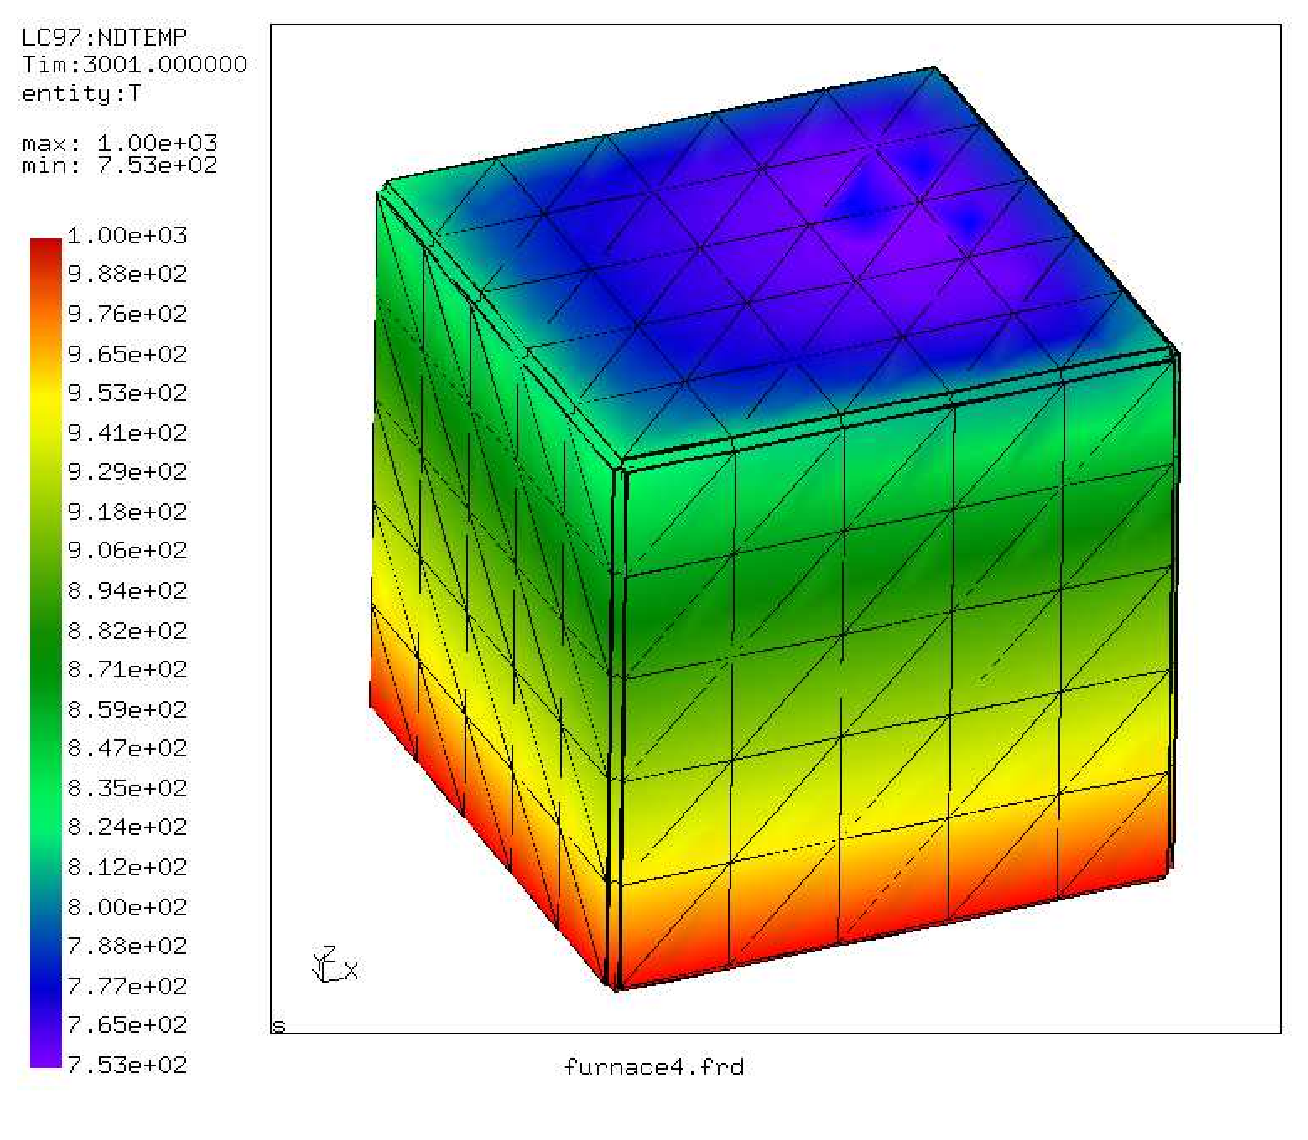
\epsfig{file=furntemp.eps,width=9cm}
\caption{\label{furntemp}Temperature distribution at t=3001 s}
\end{figure}

\begin{figure}
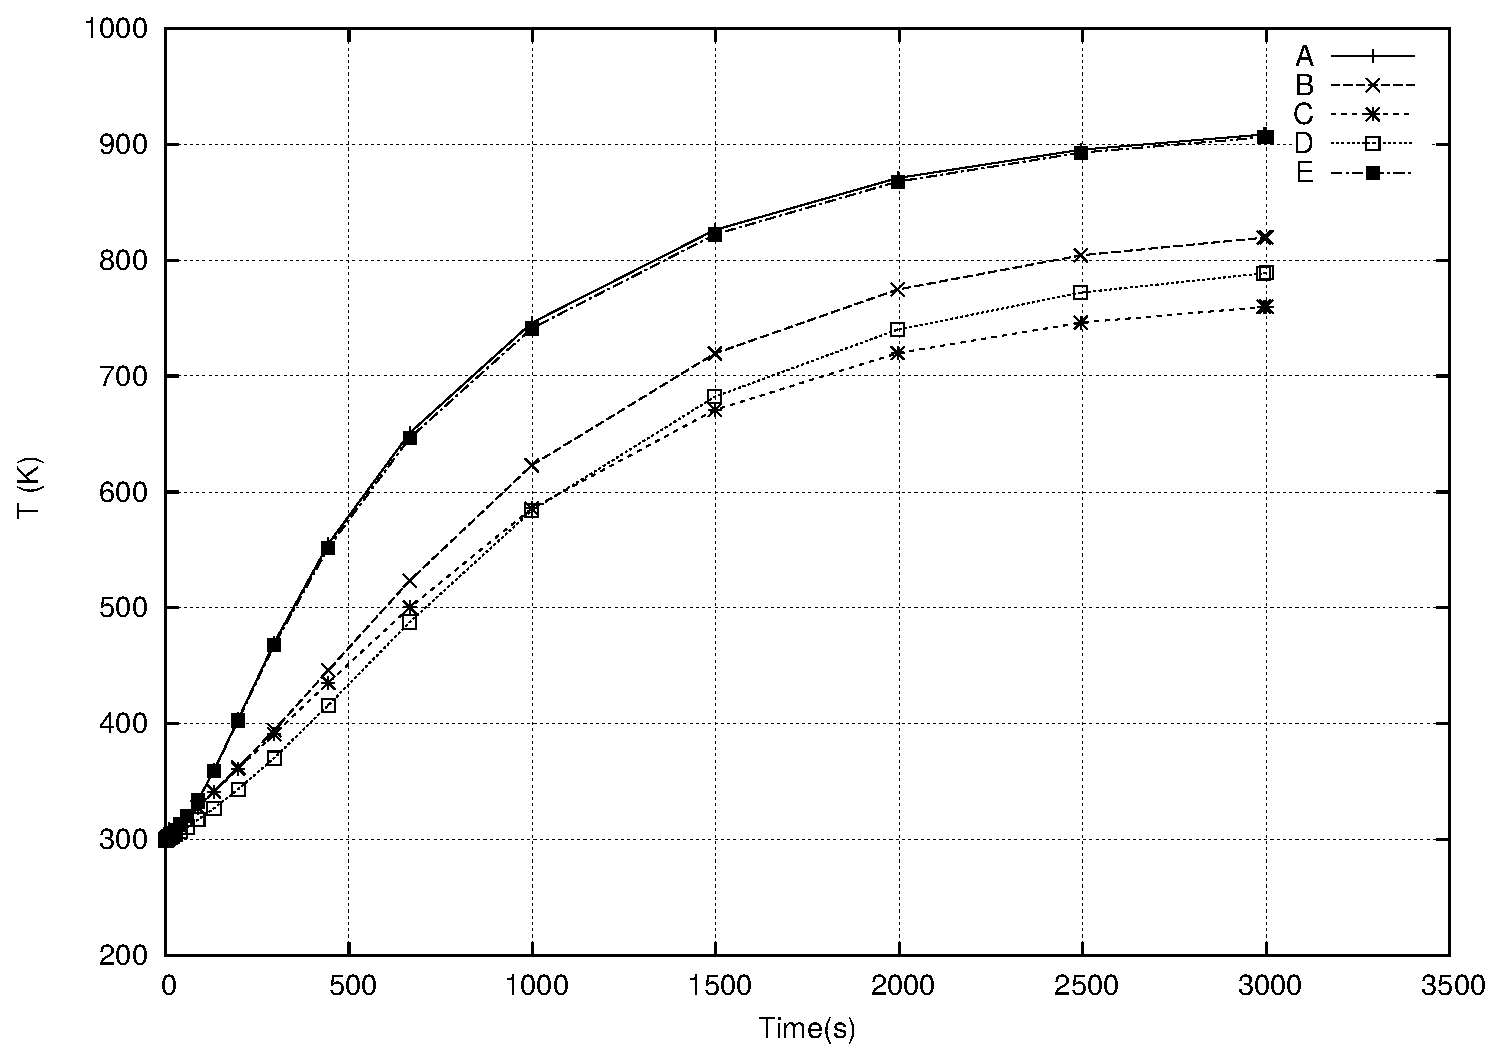
\epsfig{file=furn2D.eps,width=9cm}
\caption{\label{furn2D}Temperature at selected positions}
\end{figure}

The second and third block define the internal cavity radiation in the
furnace for the top and the sides. The fourth block defines the radiation of
the top face of the top plate of the furnace towards the environment, which is
kept at 300 K. The emissivity of the top plate is 0.8.

Next come the film conditions. Forced convection is defined for the top face
of the top plate of the furnace with a convection coefficient $h=25 \mathrm{W/mK}$. The
first line underneath the *FILM keyword indicates that the second face of
element 51 interacts through forced convection with (fluid)node 604. The last
entry in this line is the convection coefficient. So for each face interacting
with the fluid an appropriate fluid node must be specified with which the
interaction takes place.

Finally, the *NODE FILE card makes sure that the temperature is stored in the
.frd file and the *NODE PRINT card takes care that the fluid temperature is
stored in the .dat file.

The complete input deck is part of the test examples of CalculiX (furnace.inp). For the
present analysis a second step was appended keeping the bottom temperature
constant for an additional 3000 seconds. 

What happens during the calculation? The walls and top of the furnace heat up
due to conduction in the walls and radiation from the bottom. However, the top
of the furnace also loses heat through radiation with the environment and
convection with the fluid. Due to the interaction with the fluid the temperature
is asymmetric: at the inlet the fluid is cool and the furnace will lose more
heat than at the outlet, where the temperature of the fluid is higher and the
temperature difference with the furnace is smaller. So due to convection we
expect a temperature increase from inlet to outlet. Due to conduction we
expect a temperature minimum in the middle of the top. Both effects are
superimposed. The temperature distribution at $t=3001 \mathrm{s}$ is shown in
Figure \ref{furntemp}. There is a temperature gradient from the bottom of the
furnace towards the top. At the top the temperature is indeed not
symmetric. This is also shown in Figure \ref{furn2D}, where the temperature of
locations A, B, C, D and E is plotted as a function of time.

Notice that steady state conditions have not been reached yet. Also note that
2D elements (such as shell elements) are automatically expanded into 3D
elements with the right thickness. Therefore, the pictures, which were plotted
from within CalculiX GraphiX, show 3D elements.

\subsection{Seepage under a dam}

In this section, groundwater flow under a dam is analyzed. The geometry of the
dam is depicted in Figure \ref{damgeo} and is taken from exercise 30 in
Chapter 1 of \cite{Harr}. All length measurements are in feet (0.3048 m). The
water level upstream of the dam is 20 feet high, on the downstream side it is
5 feet high. The soil underneath the dam is anisotropic. Upstream the
permeability  is
characterized by $k_1= 4 k_2 = 10^{-2} \text{cm}/\text{s}$, downstream we have
$25 k_3 = 100 k_4  =  10^{-2} \text{cm}/\text{s}$. Our primary interest is the
hydraulic gradient, i.e. $ \nabla h$ since this is a measure whether or
not piping will occur. Piping means that the soil is being carried away by the
groundwater flow (usually at the downstream side) and constitutes an instable
condition. As a rule of thumb, piping will occur if the hydraulic gradient is
about unity.

From Section \ref{stationarygroundwaterflow} we know that the equations
governing stationary groundwater flow are the same as the heat equations. The
equivalent quantity of the total head is the temperature and of the velocity
it is the heat flow. For the finite element analysis SI units were taken, so
feet was converted into meter. Furthermore, a vertical impermeable wall was
assumed far upstream and far downstream (actually, 30 m upstream from the
middle point of the dam and 30 m downstream).

Now, the boundary conditions are:

\begin{enumerate}
\item
the dam, the left and right vertical boundaries upstream and downstream, and
the horizontal limit at the bottom are impermeable. This means that the
water velocity perpendicular to these boundaries is zero, or, equivalently,
the heat flux.
\item
taking the reference for the z-coordinate in the definition of total head at
the bottom of the dam (see Equation \ref{deftotalhead} for the definition of
total head), and assuming that the atmospheric pressure $p_0$ is
zero, the total head upstream is 28 feet and downstream it is 13 feet. In the
thermal equivalent this corresponds to temperature boundary conditions.
\end{enumerate}

The input deck is summarized in Figure \ref{daminp}. The complete deck is part
of the example problems. The problem is really two-dimensional and
consequently qu8 elements were used for the mesh generation within CalculiX
GraphiX. To obtain a higher resolution immediately adjacent to the dam a bias
was used (the mesh can be seen in Figure \ref{dam1}). 

\begin{figure}
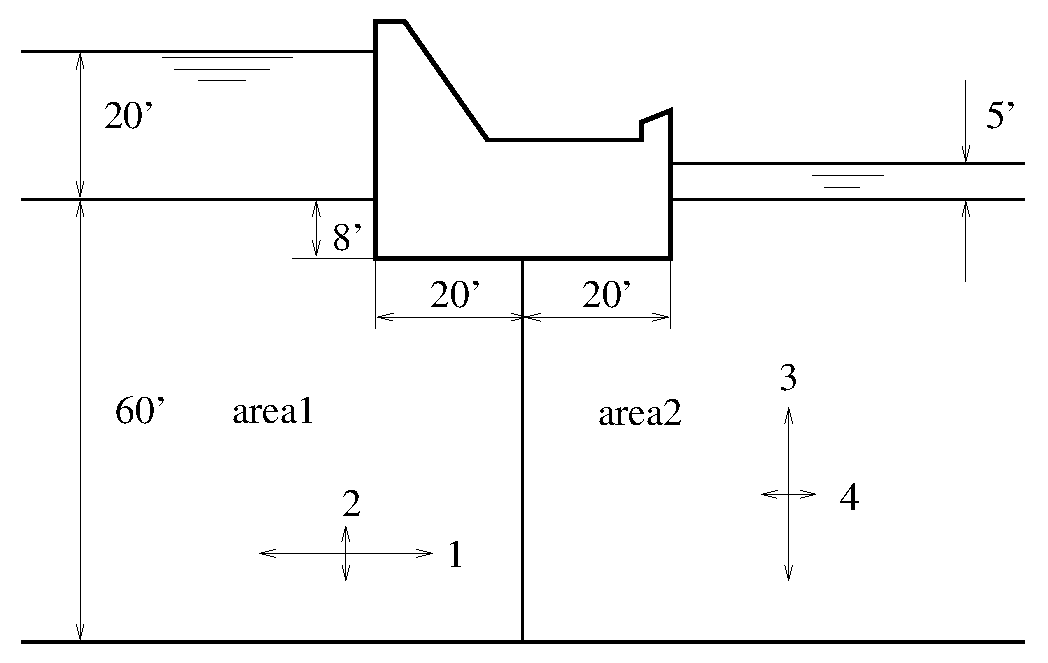
\epsfig{file=dam.eps,width=11cm}
\caption{\label{damgeo}Geometry of the dam}
\end{figure}

\begin{figure}
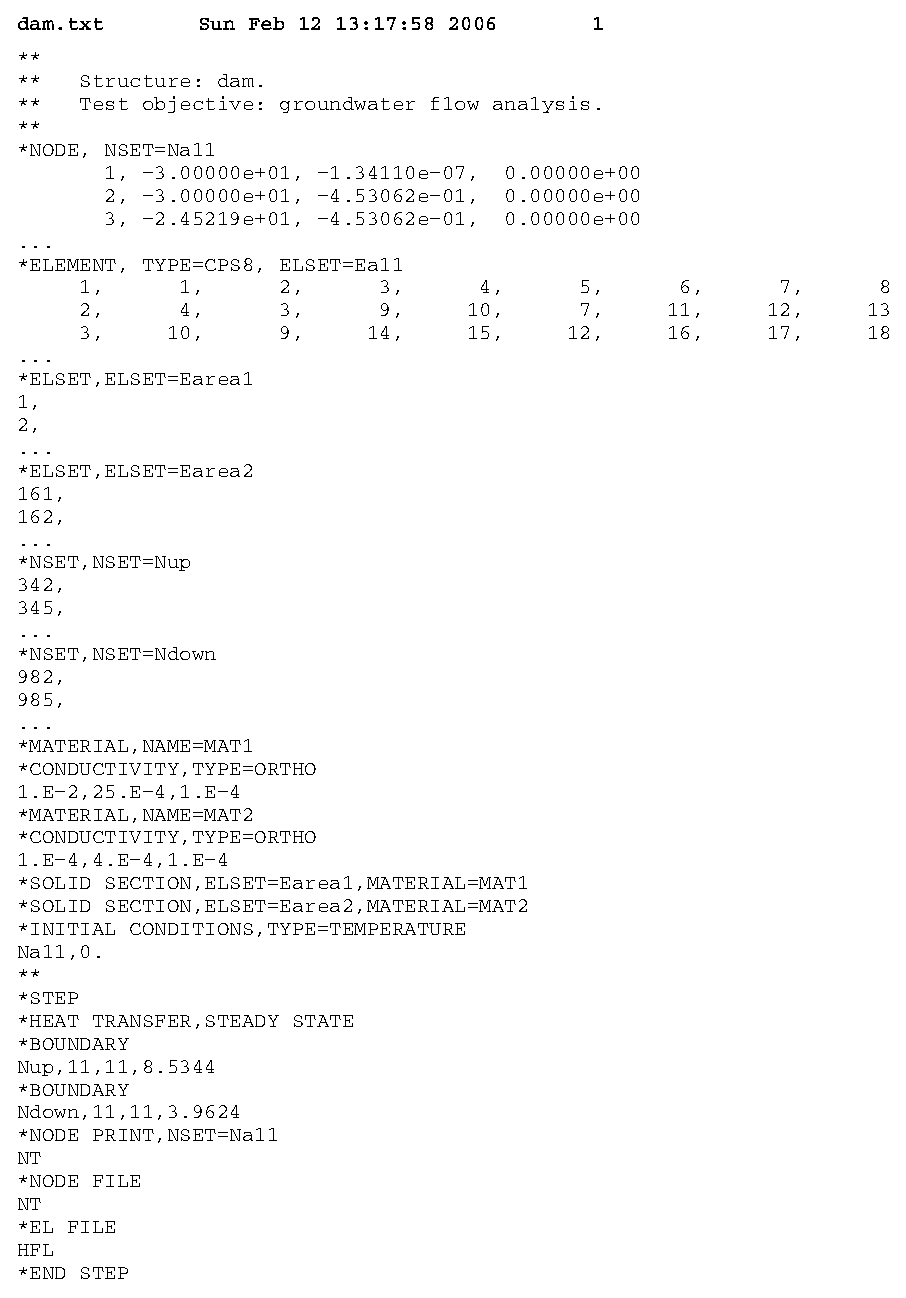
\epsfig{file=daminp.eps,width=11cm}
\caption{\label{daminp}Input deck of the dam problem}
\end{figure}

\begin{figure}
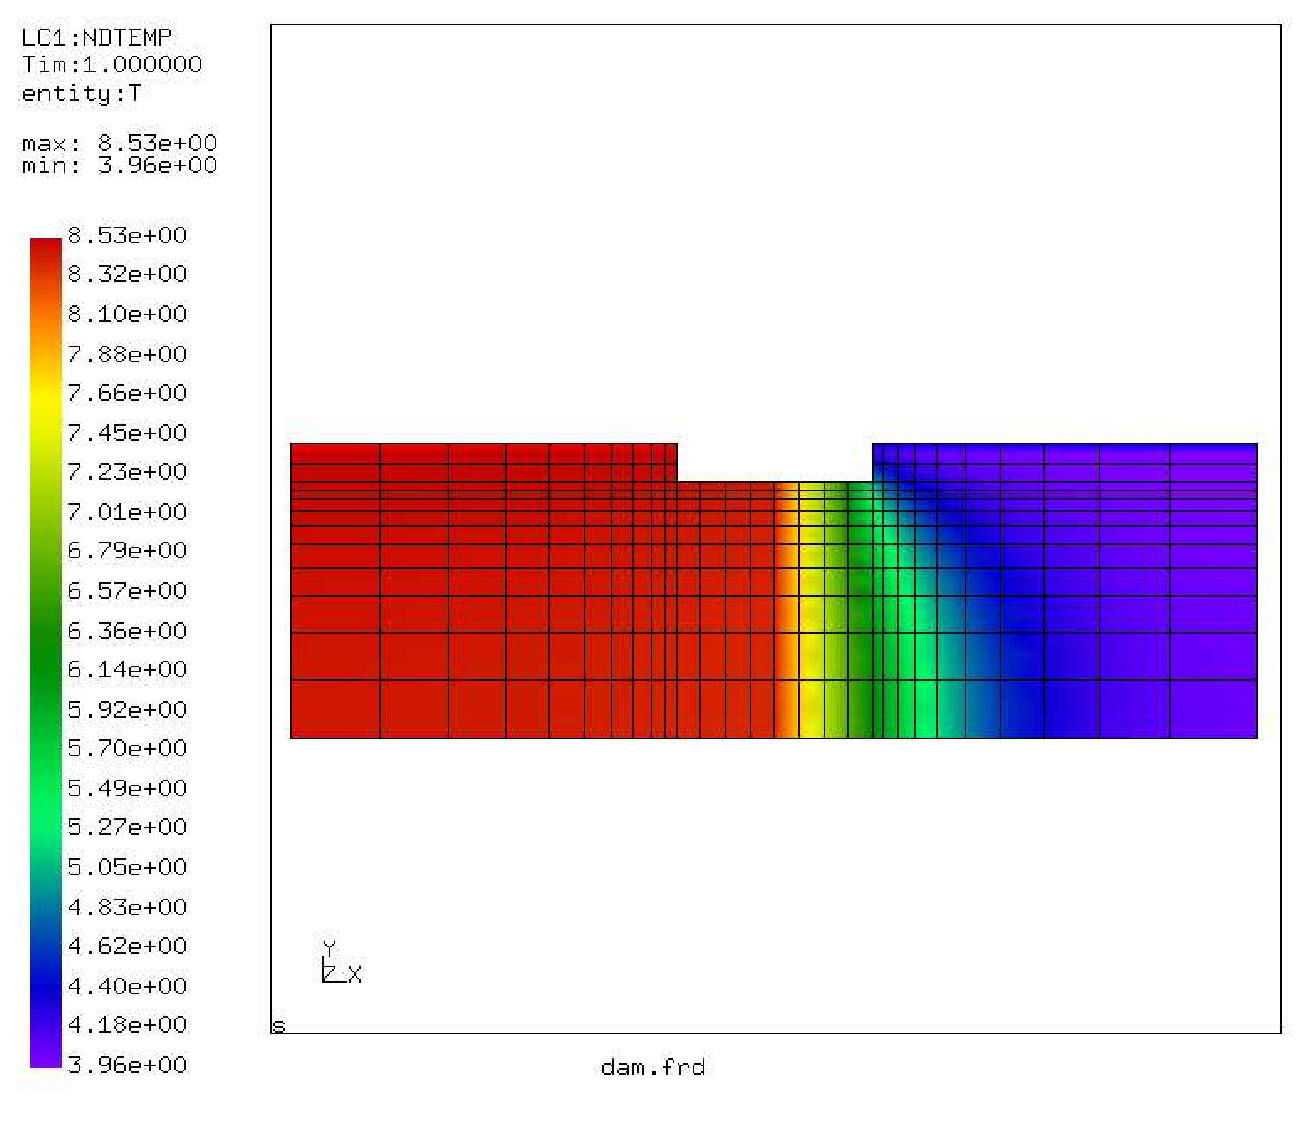
\epsfig{file=dam1.eps,width=10cm}
\caption{\label{dam1}Total head}
\end{figure}

\begin{figure}
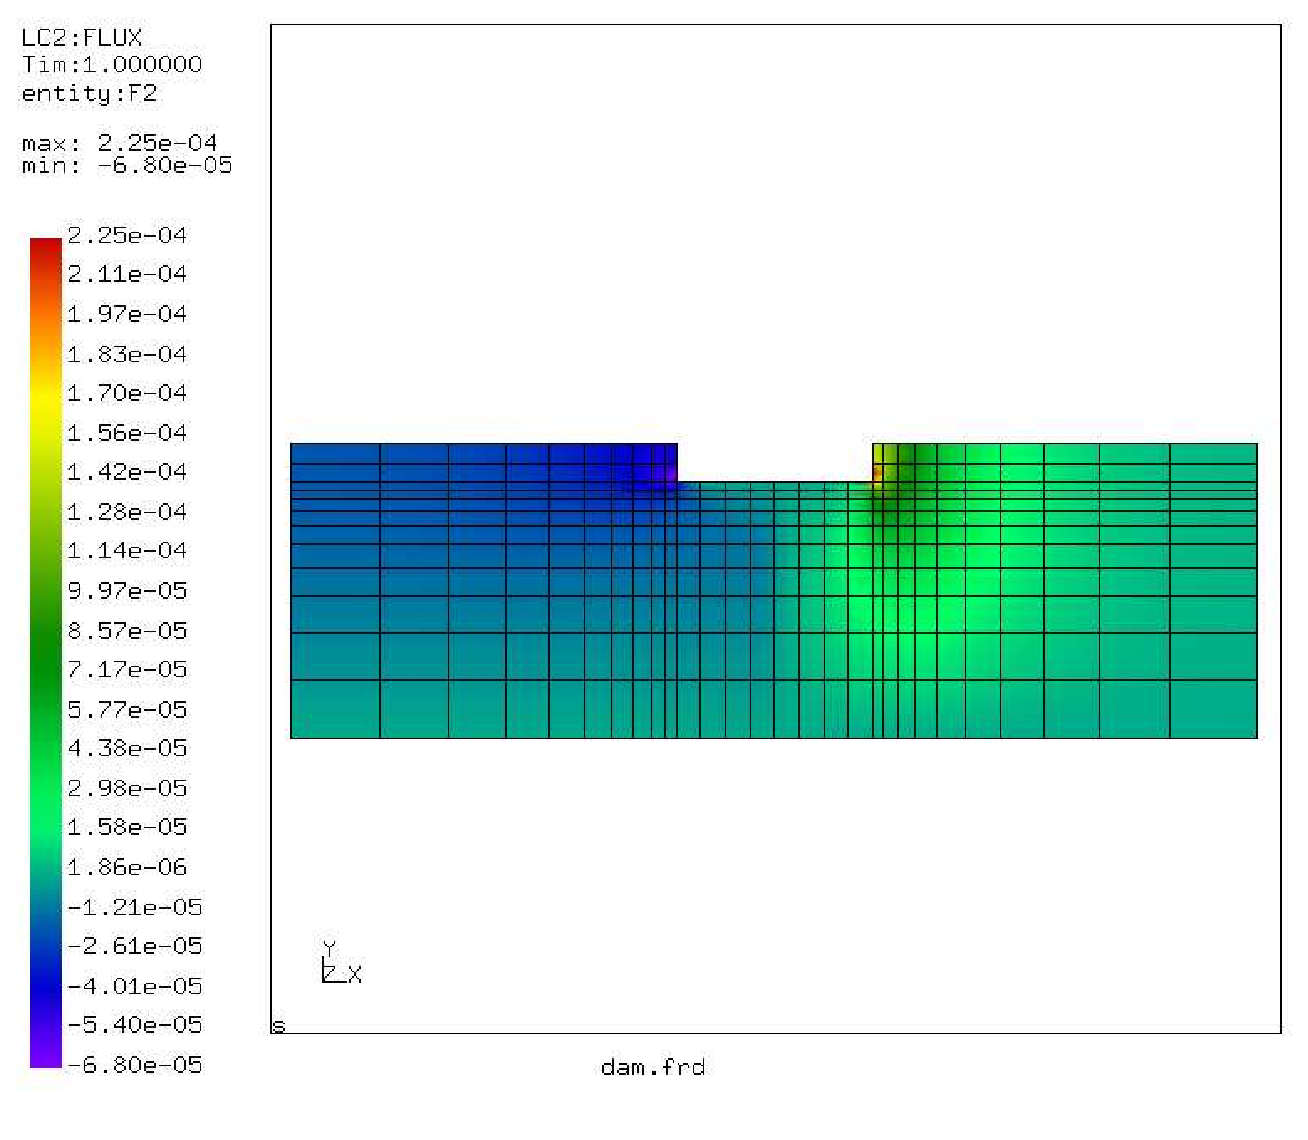
\epsfig{file=dam2.eps,width=10cm}
\caption{\label{dam2}Discharge velocity in y-direction}
\end{figure}

At the start of the deck the nodes are defined and the topology of the
elements. The qu8 element type in CalculiX GraphiX is by default translated
by the send command into a S8 (shell) element in CalculiX CrunchiX. However, a plane element is
here more appropriate. Since the calculation at stake is thermal and not
mechanical, it is really immaterial whether one takes plane strain (CPE8) or
plane stress (CPS8) elements. With the *ELSET keyword the element sets for the
two different kinds of soil are defined. The nodes on which the constant total
head is to be applied are defined by *NSET cards. The permeability of the soil
corresponds to the heat conduction coefficient in a thermal analysis. Notice
that the permeability is defined to be orthotropic, using the
*CONDUCTIVITY,TYPE=ORTHO card. The values beneath this card are the
permeability in x, y and z-direction (SI units: m/s). The value for the
z-direction is actually immaterial, since no gradient is expected in that
direction. The *SOLID SECTION card is used to assign the
materials to the appropriate soil regions. The *INITIAL CONDITIONS card is not
really needed, since the calculation is stationary, however, CalculiX CrunchiX
formally needs it in a heat transfer calculation.

Within the step a *HEAT TRANSFER, STEADY STATE calculation is selected without
any additional time step information. This means that the defaults for the step
length (1) and initial increment size (1) will be taken. With the *BOUNDARY
cards the total head upstream and downstream is defined (11 is the temperature
degree of freedom). Finally, the *NODE
PRINT, *NODE FILE and *EL FILE cards are used to define the output: NT is the
temperature, or, equivalently, the total head (Figure \ref{dam1}) , and HFL is the heat flux, or,
equivalently, the groundwater flow velocity (y-component in Figure \ref{dam2}). 

Since the permeability upstream is high, the total head gradient is small. The
converse is true downstream. The flow velocity is especially important
downstream. There it reaches values up to $2.25 \times 10^{-4}$ m/s (the red
spot in Figure \ref{dam2}), which
corresponds to a hydraulic gradient of about 0.56, since the permeability in
y-direction downstream is $4 \times 10^{-4}$ m/s. This is smaller than 1, so
no piping will occur. Notice that the velocity is naturally highest
immediately next to the dam.

This example shows how seepage problems can be solved by using the heat
transfer capabilities in CalculiX GraphiX. The same applies to any other
phenomenon governed by a Laplace-type equation. 

\subsection{Capacitance of a cylindrical capacitor}

\begin{figure}
\begin{center}
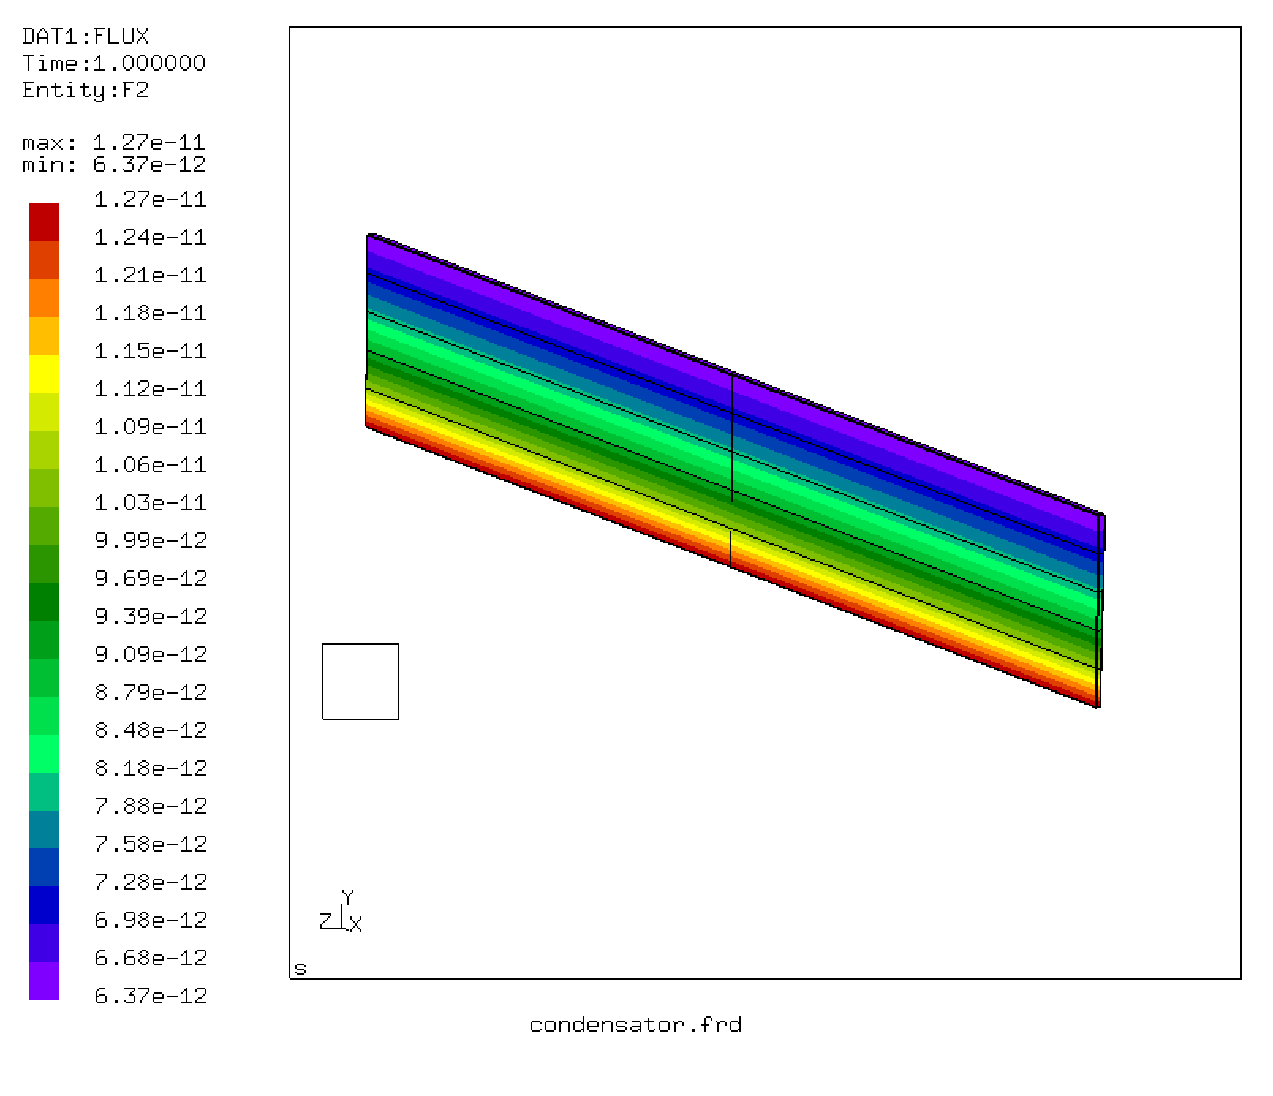
\epsfig{file=capacitor.eps,width=9cm}
\caption{\label{capacitor}Heat flux in the capacitor's thermal analogy}
\end{center}
\end{figure}

In this section the capacitance of a cylindrical capacitor is calculated with
inner radius 1 m, outer radius 2 m and length 10 m. The capacitor is filled
with air, its permittivity is $\epsilon_0=8.8542 \times 10^{-12} ~
\text{C}^2/\text{Nm}^2$. An extract of the input deck, which is part of the
test example suite, is shown below:

\begin{verbatim}
*NODE, NSET=Nall
...
*ELEMENT, TYPE=C3D20, ELSET=Eall
...
*NSET,NSET=Nin 
1, 
2, 
...
*NSET,NSET=Nout 
57, 
58, 
...
*SURFACE,NAME=S1,TYPE=ELEMENT
6,S3
1,S3
*MATERIAL,NAME=EL
*CONDUCTIVITY
8.8541878176e-12
*SOLID SECTION,ELSET=Eall,MATERIAL=EL
*STEP
*HEAT TRANSFER,STEADY STATE
*BOUNDARY
Nin,11,11,2.
Nout,11,11,1.
*EL FILE
HFL
*SECTION PRINT,SURFACE=S1
FLUX
*END STEP

\end{verbatim}

As explained in Section \ref{electrostatics} the capacitance can be
calculated by determining the total heat flux through one of the capacitor's
surfaces due to a unit temperature difference between the surfaces. The material in between the
surfaces of the capacitor is assigned a conductivity equal to its
permittivity. Here, only one degree of the capacitor has been modeled. In
axial direction the mesh is very coarse, since no variation of the temperature is expected. Figure
\ref{capacitor} shows that the heat flux at the inner radius is $1.27 \times
10^{-11} $ W/m$^2$ . This corresponds to a total heat flow of $7.98 \time
10^{-10} $ W. The analytical formula for the capacitor yields $2 \pi \epsilon_0
/ \ln (2) = 8.0261 \time 10^{-10}$ C/V. 

The total flux through the inner surface S1 is also stored in the .dat file because of
the \htmlref{*SECTION PRINT}{sectionprint} keyword card in the input deck. It
amounts to $-2.217 \times 10^{-12}$ W. This value is negative, because the
flux is entering the space in between the capacitor's surfaces. Since only one
degree was modeled, this value has to be multiplied by 360 and yields the same
value as above.


\subsection{Hydraulic pipe system}

In CalculiX it is possible to perform steady-state hydraulic and aerodynamic network
calculations, either as stand-alone applications, or together with mechanical
and/or thermal calculations of the adjacent structures. Here, a stand-alone
hydraulic network discussed in \cite{Berlamont1}  is analyzed. The input deck pipe.f can be found in the test
suite. 

\begin{figure}
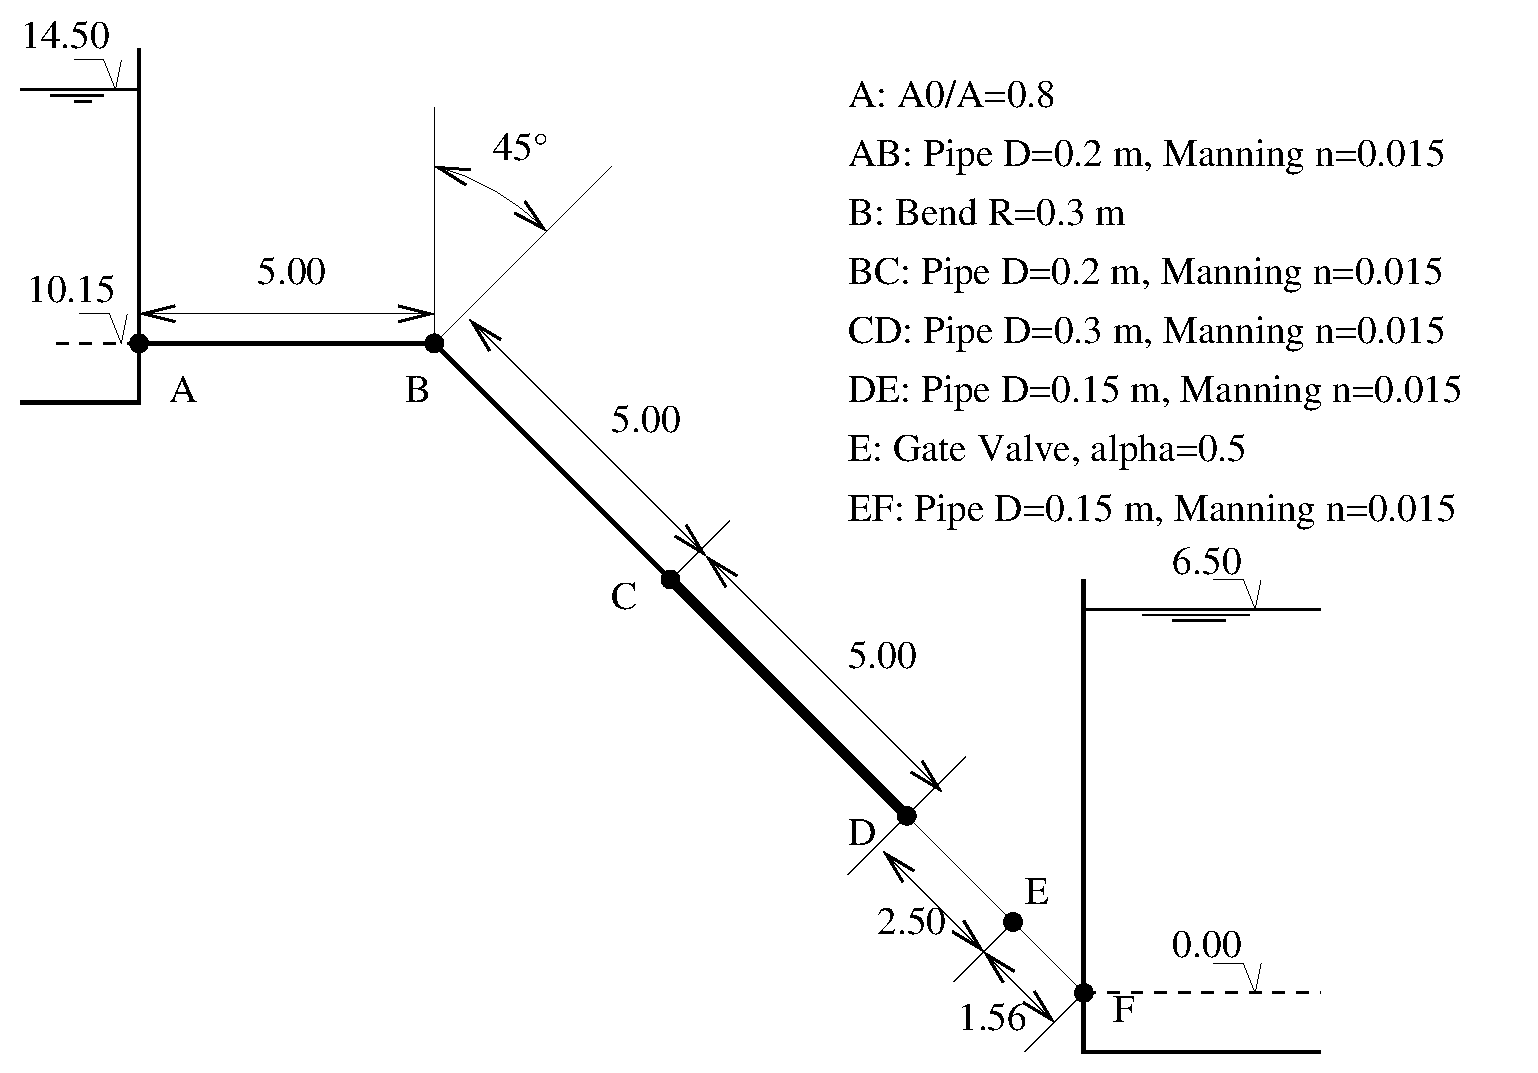
\epsfig{file=geopipe.eps,width=12cm}
\caption{\label{geopipe}Geometry of the hydraulic network}
\end{figure}

The geometry of the network is shown in Figure \ref{geopipe}. It is a linear
network consisting of:

\begin{itemize}
\item an upstream reservoir with surface level at 14.5 m
\item an entrance with a contraction of 0.8
\item a pipe with a length of 5 m and a diameter of 0.2 m
\item a bend of 45 $^o$ and a radius of 0.3 m
\item a pipe with a length of 5 m and a diameter of 0.2 m
\item a pipe with a length of 5 m and a diameter of 0.3 m
\item a pipe with a length of 2.5 m and a diameter of 0.15 m
\item a gate valve in E with $\alpha$ = 0.5
\item a pipe with a length of 1.56 m and a diameter of 0.15 m
\item an exit in a reservoir with surface level at 6.5 m
\end{itemize}

All pipes are characterized by a Manning friction coefficient n=0.015. The
input deck looks like: 

\begin{verbatim}
**
**   Structure: pipe connecting two reservoirs.
**   Test objective: hydraulic network.
**
*NODE,NSET=NALL
2,0.,0.,14.5
3,0.,0.,14.5
4,0.,0.,12.325
...
26,14.9419,0.,6.5
*ELEMENT,TYPE=D,ELSET=EALL
1,0,2,3
2,3,4,5
...
13,25,26,0
*MATERIAL,NAME=WATER
*DENSITY
1000.
*FLUID CONSTANTS
4217.,1750.E-6,273.
*ELSET,ELSET=E1
2
*ELSET,ELSET=E2
3,5
*ELSET,ELSET=E3
4
*ELSET,ELSET=E4
6
*ELSET,ELSET=E5
7
*ELSET,ELSET=E6
8
*ELSET,ELSET=E7
9,11
*ELSET,ELSET=E8
10
*ELSET,ELSET=E9
12
*ELSET,ELSET=E10
1,13
*FLUID SECTION,ELSET=E1,TYPE=PIPE ENTRANCE,MATERIAL=WATER
0.031416,0.025133
*FLUID SECTION,ELSET=E2,TYPE=PIPE MANNING,MATERIAL=WATER
0.031416,0.05,0.015
*FLUID SECTION,ELSET=E3,TYPE=PIPE BEND,MATERIAL=WATER
0.031416,1.5,45.,0.4
*FLUID SECTION,ELSET=E4,TYPE=PIPE ENLARGEMENT,MATERIAL=WATER
0.031416,0.070686
*FLUID SECTION,ELSET=E5,TYPE=PIPE MANNING,MATERIAL=WATER
0.070686,0.075,0.015
*FLUID SECTION,ELSET=E6,TYPE=PIPE CONTRACTION,MATERIAL=WATER
0.070686,0.017671
*FLUID SECTION,ELSET=E7,TYPE=PIPE MANNING,MATERIAL=WATER
0.017671,0.0375,0.015
*FLUID SECTION,ELSET=E8,TYPE=PIPE GATE VALVE,MATERIAL=WATER
0.017671,0.5
*FLUID SECTION,ELSET=E9,TYPE=PIPE ENLARGEMENT,MATERIAL=WATER
0.017671,1.E6
*FLUID SECTION,ELSET=E10,TYPE=PIPE INOUT,MATERIAL=WATER
*BOUNDARY
3,2,2,1.E5
25,2,2,1.E5			  
*STEP
*HEAT TRANSFER,STEADY STATE
*DLOAD
EALL,GRAV,9.81,0.,0.,-1.
*NODE PRINT,NSET=NALL
U
*END STEP
\end{verbatim}

In CalculiX linear networks are modeled by means of 3-node network elements
(D-type elements). In the corner nodes of the element the temperature and the
pressure are unknown. They are assigned to the degrees of freedom 0 and 2,
respectively. In the midside node the mass flux is unknown and is assigned to
degree of freedom 1. The properties of the network elements are defined by the
keyword \htmlref{*FLUID SECTION}{fluidsection}. They are treated extensively
in Section \ref{fluidsectiontypesgases} (gases),
\ref{fluidsectiontypesliquids} (liquid pipes) and \ref{fluidsectiontypeschannels}
(liquid channels). For the network at stake we need:

\begin{itemize}
\item a dummy network entrance element expressing that liquid is entering the
  network (element 1). It is characterized by a node number 0 as first node
\item a network element of type PIPE ENTRANCE at location A (element 2). This element also
  takes the water depth into account. Notice that there is no special
  reservoir element. Differences in water level can be taken into account in
  any element type by assigning the appropriate coordinates to the corner nodes
  of the element.
\item a network element of type PIPE MANNING for the pipe between location A and
  B (element 3)
\item a network element of type PIPE BEND for the bend at location B (element 4)
\item a network element of type PIPE MANNING for the pipe between location B and
  C (element 5)
\item a network element of type PIPE ENLARGEMENT for the increase of diameter at
  location C (element 6)
\item a network element of type PIPE MANNING for the pipe between location C and
  D (element 7)
\item a network element of type PIPE CONTRACTION to model the decrease in
  diameter at location D (element 8)
\item a network element of type PIPE MANNING for the pipe between location D and
  E (element 9)
\item a network element of type PIPE GATE VALVE for the valve at location E
  (element 10)
\item a network element of type PIPE MANNING for the pipe between location E and
  F (element 11)
\item a network element of type PIPE ENLARGEMENT for the exit in the
  reservoir (element 12). Indeed, there is no special reservoir entrance element. A
  reservoir entrance has to be modeled by a large diameter increase.
\item a dummy network exit element expressing that liquid is leaving the
  network (element 13)
\end{itemize}

In the input deck, all these elements are defined as D-type elements, their
nodes 
have the correct coordinates and by means of *FLUID SECTION cards each element
is properly described. Notice that the dummy network entrance and exit
elements are characterized by typeless *FLUID SECTION cards. 

For a hydraulic network the material properties reduce to the density (on the \htmlref{*DENSITY}{density} card), the specific heat and the dynamic
viscosity (both on the \htmlref{*FLUID SECTION}{fluidsection} card). The
specific heat is only needed if heat transfer is being modeled. Here, this is
not the case. The dynamic viscosity of water is $1750 \times 10^{-6} \text{N
  s/m}^2$  \cite{Incropera}. The boundary conditions reduce to the atmospheric pressure in node 3 and 25, both at the
liquid surface of the reservoir. Remember that the pressure has the degree of
freedom 2 in the corner nodes of the network elements.  

Networks are only active in 
\htmlref{*COUPLED TEMPERATURE-DISPLACEMENT}{coupledtemperaturedisplacement} or \htmlref{*HEAT TRANSFER}{heattransfer}
procedures. Here, we do not take the structure into account, so a heat
transfer analysis will do. Finally, the gravity loading has to be specified,
this is indeed essential for hydraulic networks. Regarding the nodal output,
remember that NT requests degree of freedom 0, whereas U requests degrees of
freedom 1 to 3. Since we are interested in the mass flux (DOF 1 in the middle
nodes) and the pressure (DOF 2 in the corner nodes), U is selected underneath the
*NODE PRINT line. Officially, U are displacements, and that's the way they are
labeled in the .dat file.

The results in the .dat file look as follows:

\begin{verbatim}

 displacements (vx,vy,vz) for set NALL and time   1.

     2  8.9592E+01  0.0000E+00  0.0000E+00
     3  0.0000E+00  1.0000E+05  0.0000E+00
     4  8.9592E+01  0.0000E+00  0.0000E+00
     5  0.0000E+00  1.3386E+05  0.0000E+00
     6  8.9592E+01  0.0000E+00  0.0000E+00
     7  0.0000E+00  1.2900E+05  0.0000E+00
     8  8.9592E+01  0.0000E+00  0.0000E+00
     9  0.0000E+00  1.2859E+05  0.0000E+00
    10  8.9592E+01  0.0000E+00  0.0000E+00
    11  0.0000E+00  1.5841E+05  0.0000E+00
    12  8.9592E+01  0.0000E+00  0.0000E+00
    13  0.0000E+00  1.6040E+05  0.0000E+00
    14  8.9592E+01  0.0000E+00  0.0000E+00
    15  0.0000E+00  1.9453E+05  0.0000E+00
    16  8.9592E+01  0.0000E+00  0.0000E+00
    17  0.0000E+00  1.7755E+05  0.0000E+00
    18  8.9592E+01  0.0000E+00  0.0000E+00
    19  0.0000E+00  1.8361E+05  0.0000E+00
    20  8.9592E+01  0.0000E+00  0.0000E+00
    21  0.0000E+00  1.5794E+05  0.0000E+00
    22  8.9592E+01  0.0000E+00  0.0000E+00
    23  0.0000E+00  1.6172E+05  0.0000E+00
    24  8.9592E+01  0.0000E+00  0.0000E+00
    25  0.0000E+00  1.0000E+05  0.0000E+00
    26  8.9592E+01  0.0000E+00  0.0000E+00

\end{verbatim}

The mass flux in the pipe (first DOF in the midside nodes, column 1) is constant and takes the value 89.592
kg/s. This agrees well with the result in \cite{Berlamont1} of 89.4 l/s. Since
not all node and element definitions are listed it is
useful for the interpretation of the output to know that location A corresponds to node 5, location B to nodes 7-9, location C to nodes 11-13,
location D to nodes 15-17, location E to nodes 19-21 and location F to node
23. The second column in the result file is the pressure. It shows that the
bend, the valve and the contraction lead to a pressure decrease, whereas the
enlargement leads to a pressure increase (the velocity drops). 

If the structural side of the network (e.g. pipe walls) is modeled too, the
fluid pressure can be mapped automatically onto the structural element
faces. This is done by labels of type PxNP in the \htmlref{*DLOAD}{dload} card.

\subsection{Lid-driven cavity}

The lid-driven cavity is a well-known benchmark problem for viscous
incompressible fluid flow \cite{Zienkiewicz2}. The geometry at stake is shown in Figure
\ref{lidgeo}. We are dealing with a square cavity consisting of three rigid
walls with no-slip conditions and a lid moving with a tangential unit
velocity. The lower left corner has a reference static pressure of 0. We are
interested in the velocity and pressure distribution for a Reynolds number of
400. 

\begin{figure}
\begin{center}
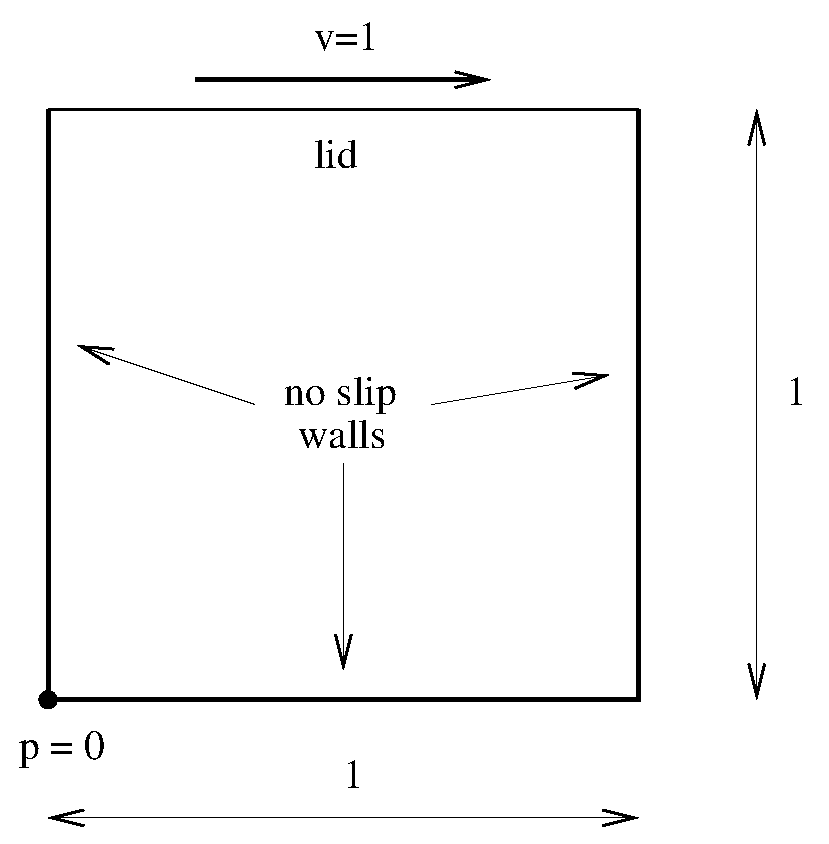
\epsfig{file=lidgeo.eps,width=10cm}
\caption{\label{lidgeo}Geometry of the lid-driven cavity}
\end{center}
\end{figure}

\begin{figure}
\begin{center}
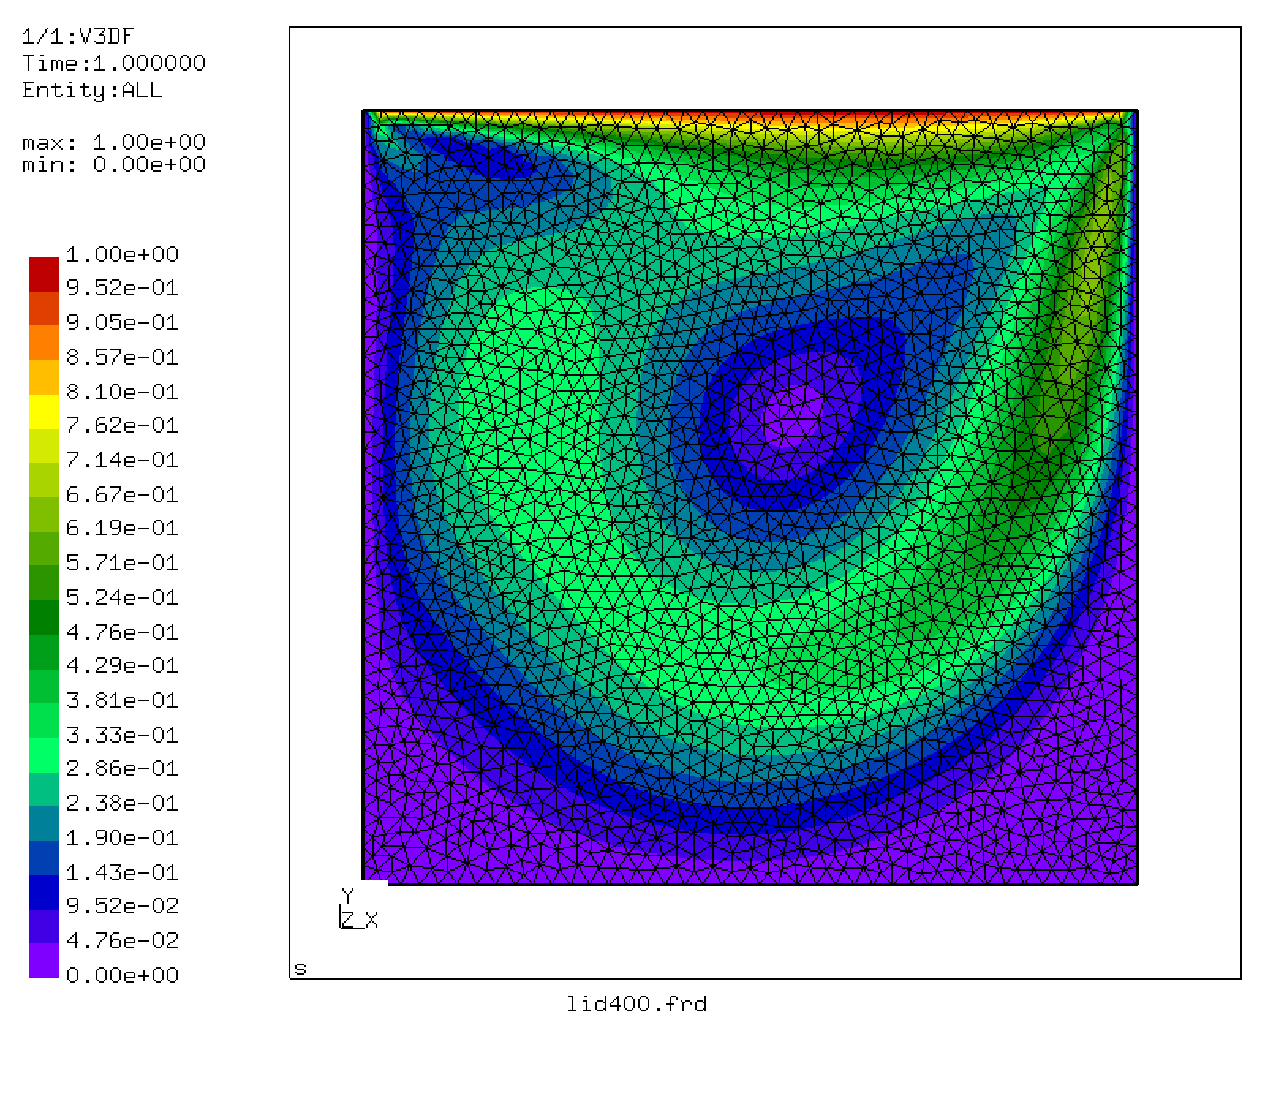
\epsfig{file=lidmeshfem.eps,width=9cm}
\caption{\label{lidmeshfem}Mesh of the lid-driven cavity}
\end{center}
\end{figure}

\begin{verbatim}
**
**   Structure: lid-driven cavity.
**   Test objective: incompressible, viscous, laminar, 3D fluid flow
**
*NODE,NSET=Nall
1,0.00000,0.00000,0.
...  
*ELEMENT,TYPE=F3D6,ELSET=Eall
1,1543,1626,1624,3918,4001,3999
...
*NSET,NSET=Nin 
1774, 
...
*NSET,NSET=Nwall 
1, 
...
*NSET,NSET=N1 
1374, 
...
*BOUNDARY
Nall,3,3,0.
Nwall,1,2,0.
Nin,2,2,0. 
1,8,8,0.
2376,8,8,0.
*MATERIAL,NAME=WATER
*DENSITY
1.
*FLUID CONSTANTS
1.,.25E-2,293.
*SOLID SECTION,ELSET=Eall,MATERIAL=WATER
*INITIAL CONDITIONS,TYPE=FLUID VELOCITY
Nall,1,0.
Nall,2,0.
Nall,3,0.
*INITIAL CONDITIONS,TYPE=PRESSURE
Nall,0.
**
*STEP,INCF=20000
*CFD,STEADY STATE
*BOUNDARY
Nin,1,1,1.
*NODE FILE,FREQUENCYF=200
VF,PSF
*END STEP

\end{verbatim}      

The input deck is listed above (this deck is also available
in the fluid test suite as file lid400.inp). Although the problem is
essentially 2-dimensional it was modeled as a 3-dimensional problem with unit
thickness since 2-dimensional fluid capabilities are not available in
CalculiX. The mesh (2D projection) is shown in Figure \ref{lidmeshfem}. It
consists of 6-node wedge elements. There is one element layer across the
thickness. This is sufficient, since the results do not vary in thickness
direction. The input deck starts with the coordinates of the nodes and the
topology of the elements. The element type for fluid volumetric elements is the same
as for structural elements with the C replaced by F (fluid): F3D6. The nodes
making up the lid and those belonging to the no-slip walls are collected into
the nodal sets Nin and Nwall, respectively. The nodal set N1 is created for
printing purposes. It contains a subset of nodes close to the lid.

The homogeneous boundary conditions (i.e. those with zero value) are listed
next underneath the *BOUNDARY keyword: The velocity in all nodes in
z-direction is zero, the velocity at the walls is zero
(no-slip condition) as well as the normal velocity at the lid. Furthermore,
the reference point in the lower left
corner of the cavity has a zero pressure (node 1 and its corresponding node
across the thickness 2376). The material definition consists of the density, the
heat capacity and the dynamic viscosity. The density is set to 1. The heat
capacity and dynamic viscosity are entered underneath the \htmlref{*FLUID
  CONSTANTS}{fluidconstants} keyword. The heat capacity is not needed
since the calculation is steady state, so its value here is irrelevant. The
value of the dynamic viscosity was chosen such that the Reynolds number is
400. The Reynolds number is defined as velocity times length divided by the
kinematic viscosity. The velocity of the lid is 1, its length is 1 and since
the density is 1 the kinematic and dynamic viscosity coincide. Consequently,
the kinematic viscosity takes the value 1/400. The material is assigned to the
elements by means of the *SOLID SECTION card.

The unknowns of the problem are the velocity and static pressure. No thermal
boundary conditions are provided, so the temperature is irrelevant. All
initial values for the unknowns are set to 0 by means o the *INITIAL
CONDITIONS,TYPE=FLUID VELOCITY and *INITIAL CONDITIONS,TYPE=PRESSURE
cards. Notice that for the velocity the initial conditions have to be
specified for each degree of freedom separately. 

The step is as usual started with the *STEP keyword. The maximum number of increments,
however, is for fluid calculations governed by the parameter INCF. For steady
state fluid calculations the keyword *CFD,STEADY STATE is to be used. The values underneath
this line are not relevant for fluid calculations, since the increment size is
automatically chosen such that the procedure is stable. The nonzero tangential
velocity of the lid is entered underneath the *BOUNDARY card. Recall that
non-homogeneous (i.e. nonzero) boundary conditions have to be defined within a
step. The step ends with a nodal print request for the velocity VF and the
static pressure PS. The printing frequency is defined to be 200 by means of the
FREQUENCYF parameter. This means, that results will be stored every 200 increments.

\begin{figure}
\begin{center}
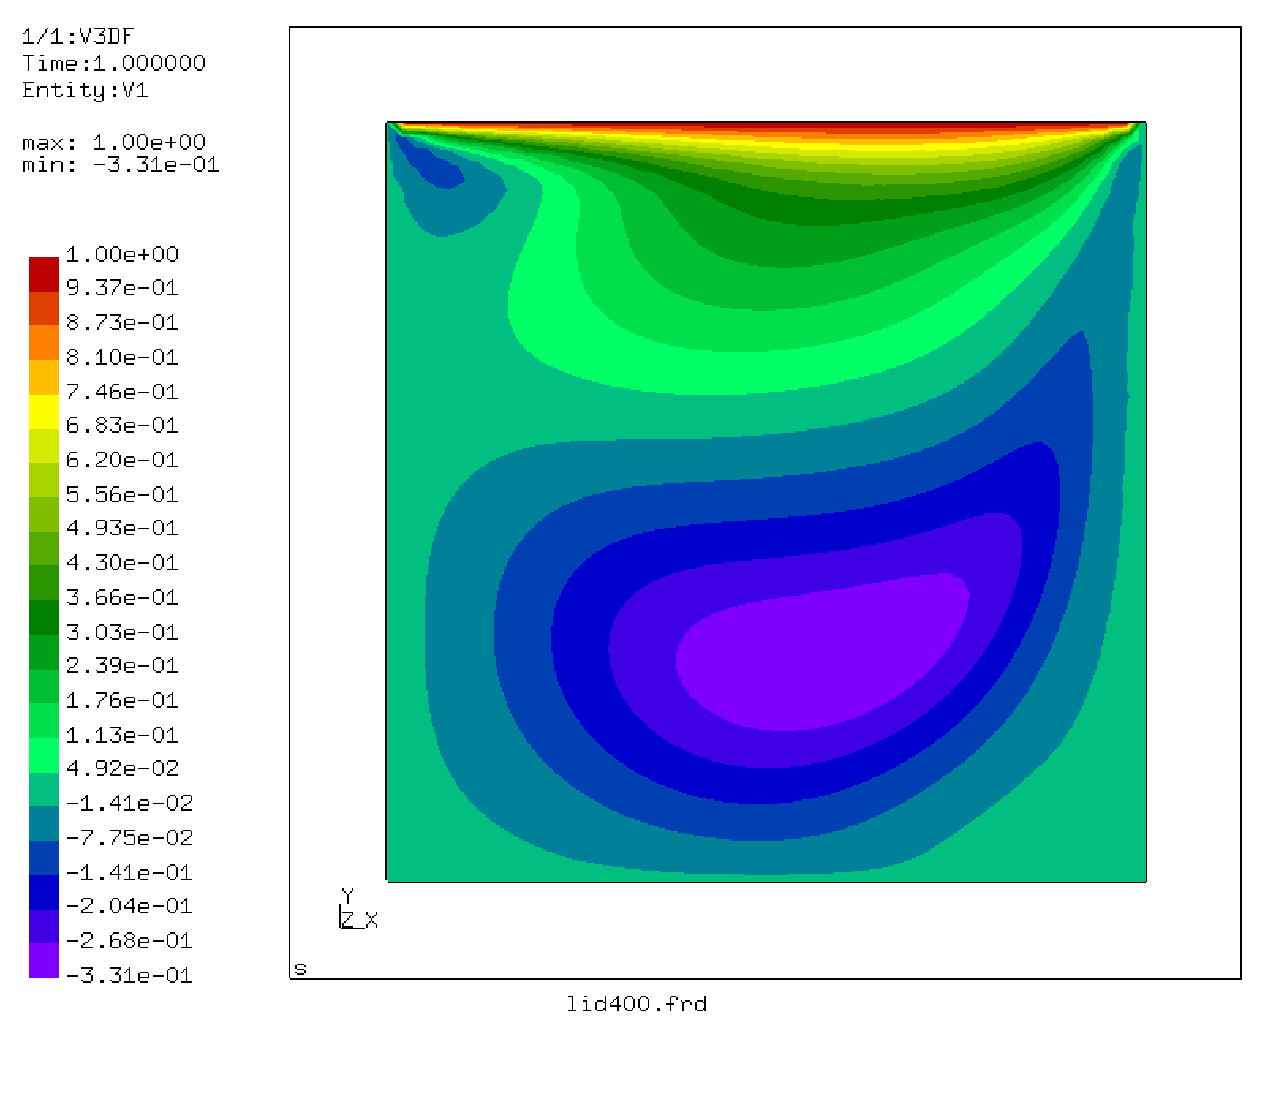
\epsfig{file=lidvelxfem.eps,width=9cm}
\caption{\label{lidvelxfem}x-component of the velocity in the lid-driven cavity}
\end{center}
\end{figure}

\begin{figure}
\begin{center}
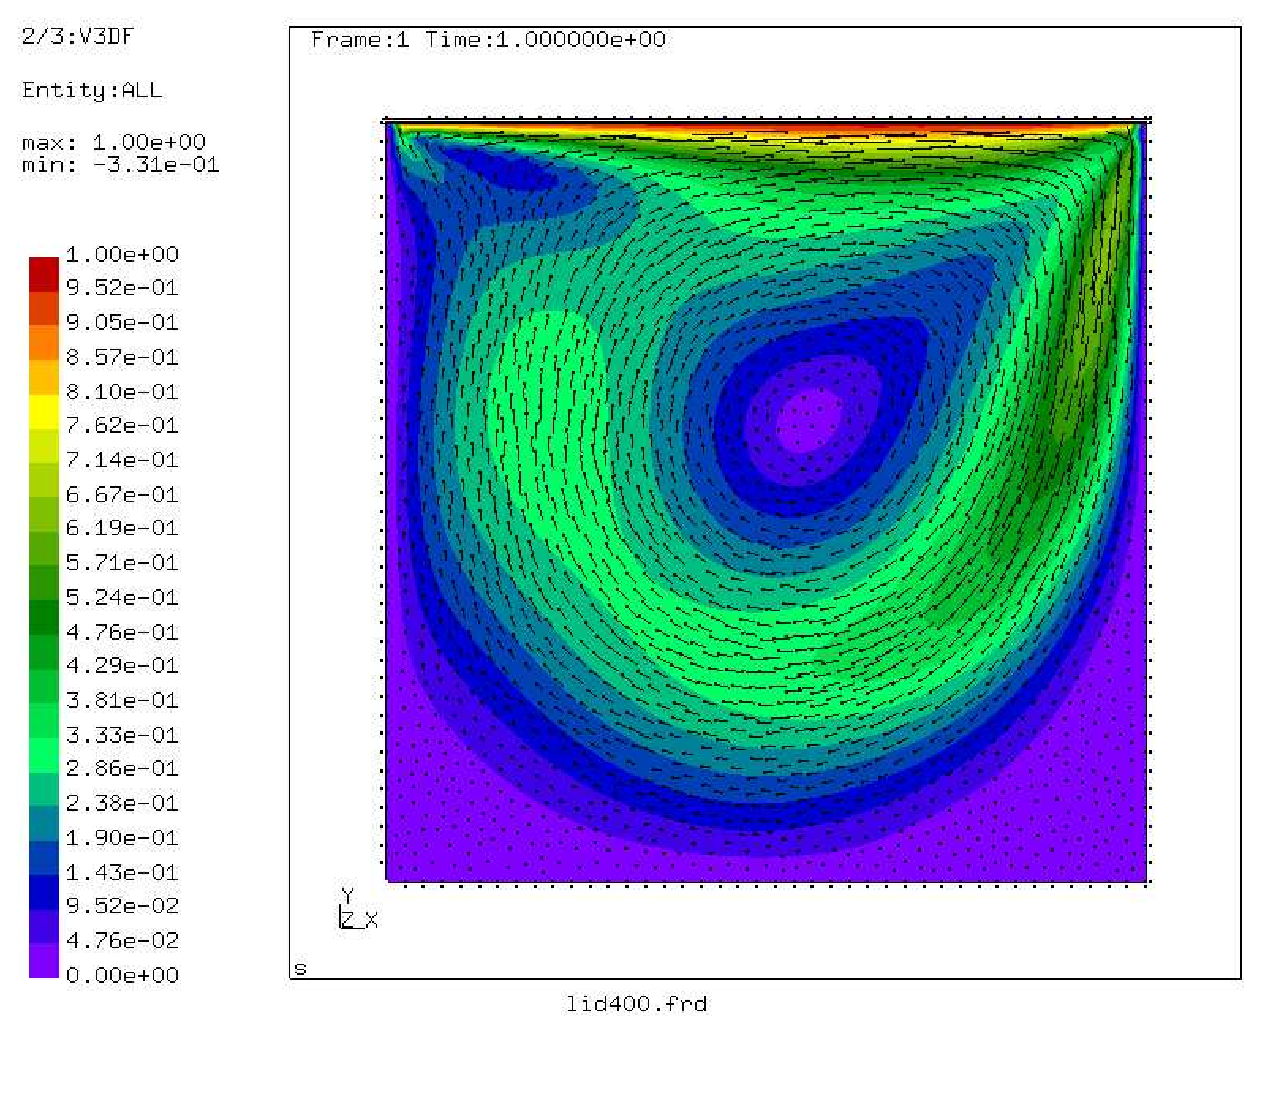
\epsfig{file=lidvelfem.eps,width=9cm}
\caption{\label{lidvelfem}Velocity distribution in the lid-driven cavity}
\end{center}
\end{figure}

\begin{figure}
\begin{center}
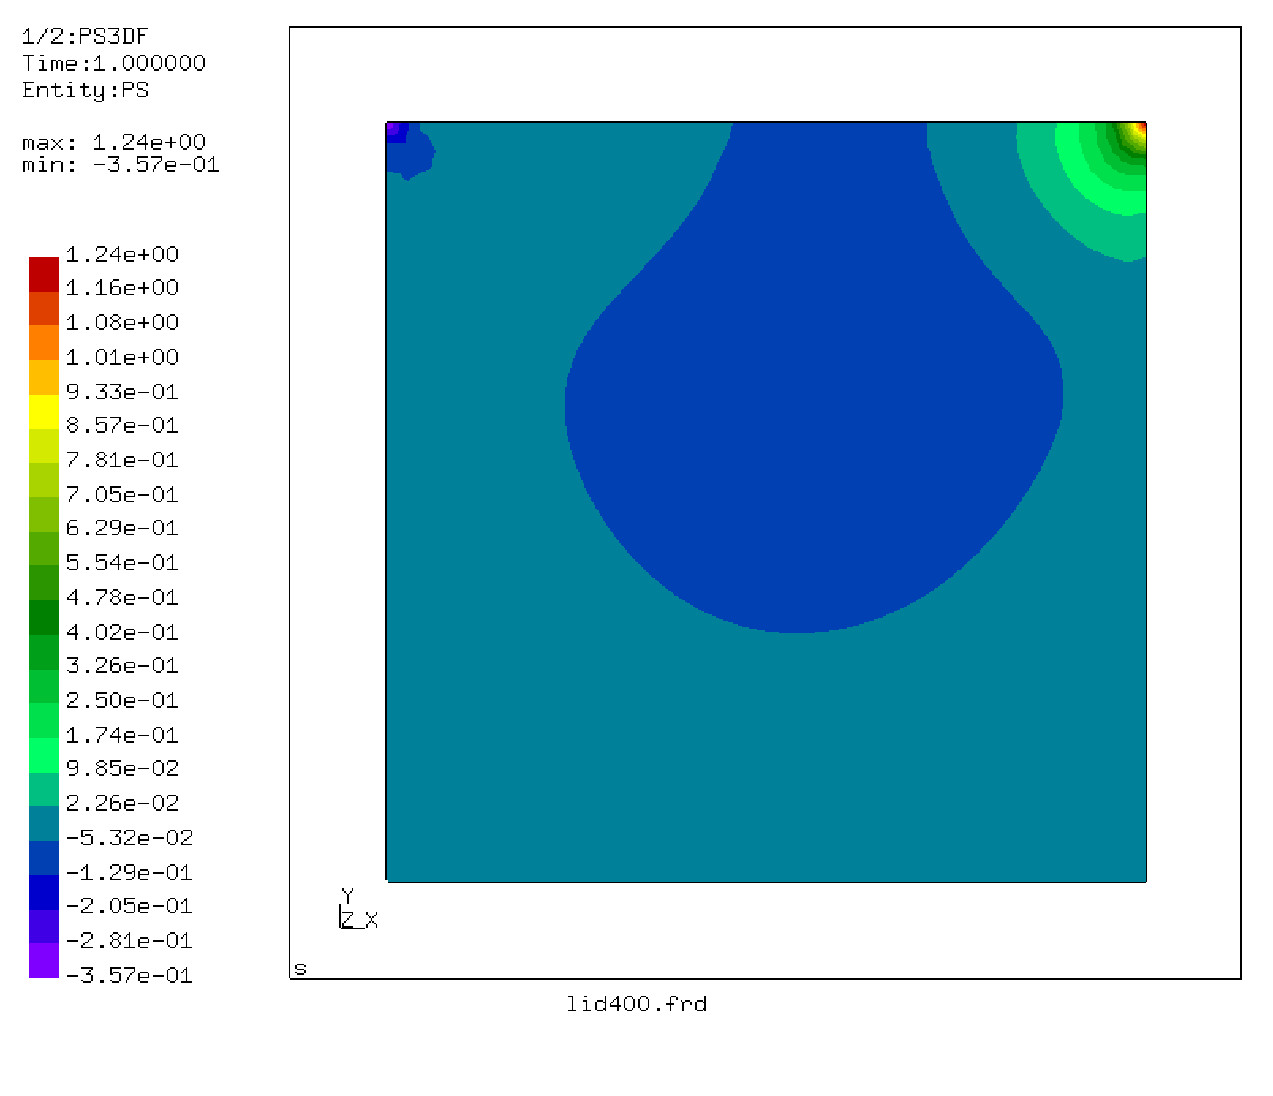
\epsfig{file=lidprefem.eps,width=9cm}
\caption{\label{lidprefem}Pressure distribution in the lid-driven cavity}
\end{center}
\end{figure}

The velocity distribution in x-direction (i.e. the direction tangential to the lid) is
shown in Figure \ref{lidvelxfem}. The smallest value (-0.33) and its location
agree very well with the results in \cite{Zienkiewicz2}. Figure \ref{lidvelfem}
shows a vector plot of the velocity. Near the lid there is a large gradient,
in the lower left and lower right corner are dead zones. The pressure plot
(Figure \ref{lidprefem}) reveals a low pressure zone in the center of the major
vortex and in the left upper corner. The right upper corner is a stagnation
point for the x-component of the velocity and is characterized by a
significant pressure built-up.

\subsection{Transient laminar incompressible Couette problem}

Another well-known problem is the incompressible laminar flow between two
parallel plates. At time zero both plates are at rest, whereas at positive
times one of the plates is moved parallel to the other plate with a velocity
of 1. The analytical solution can be found in \cite{Schlichting} in the form
of a series expansion containing the complementary error function erfc. In the
steady state regime the velocity profile is linear across the space in between
the plates. The velocity profiles at different times are shown in Figure
\ref{couette1} and compared with the analytical solution for a unity distance
between the plates and a kinematic viscosity $\nu=1$. The input deck for the
CalculiX results can be found in the test suite (couette1.inp). The figure
shows a good agreement between the numerical and analytical values, indicating
that the time integration in the CFD-implementation in CalculiX is
correct. The small deviations at small times are due to the rather course mesh.

\begin{figure}
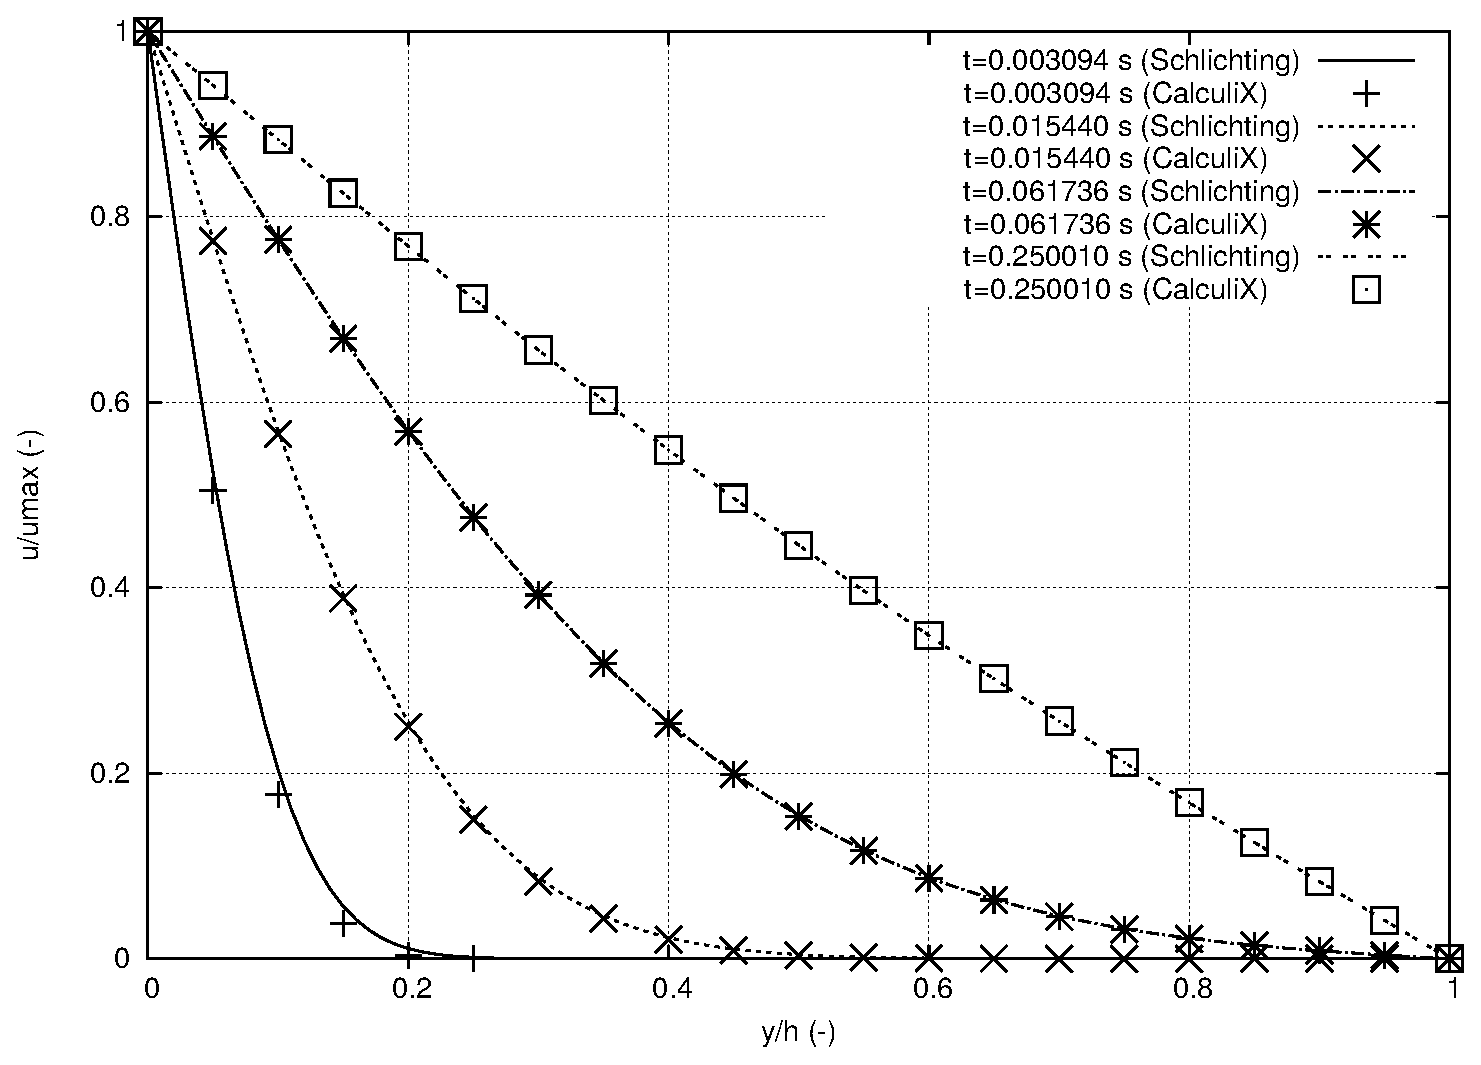
\epsfig{file=couette_transient.eps,width=8cm}
\caption{\label{couette1}Velocity across the space in between the plates for different times}
\end{figure}

\subsection{Stationary laminar inviscid compressible airfoil flow}

\begin{figure}
\begin{center}
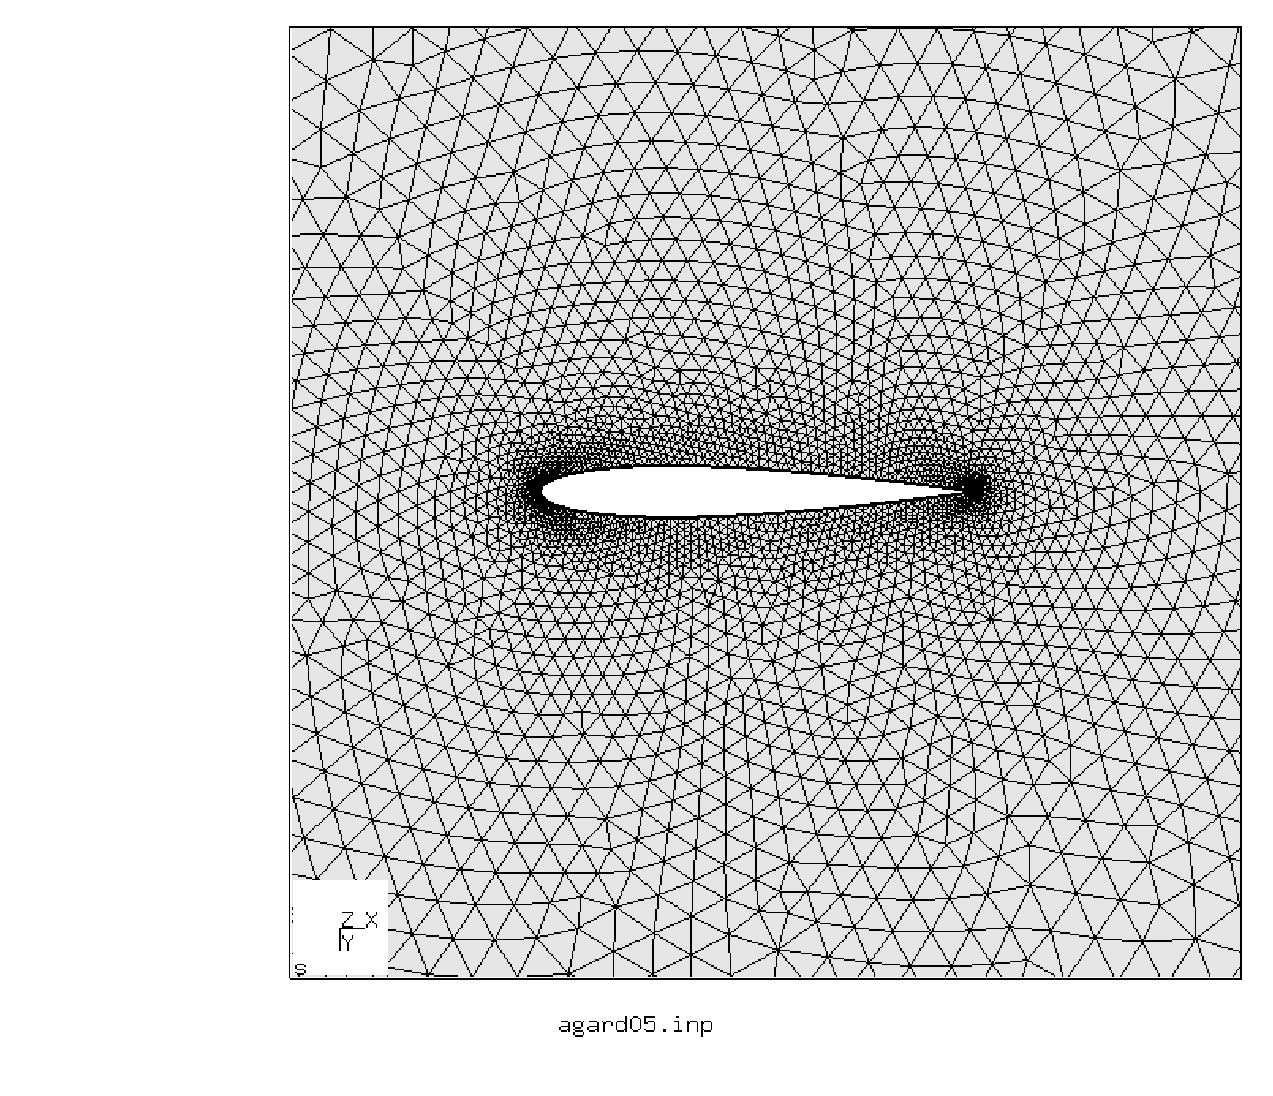
\epsfig{file=agard05.eps,width=9cm}
\caption{\label{naca012}Mesh for the naca012 airfoil flow}
\end{center}
\end{figure}

\begin{figure}
\begin{center}
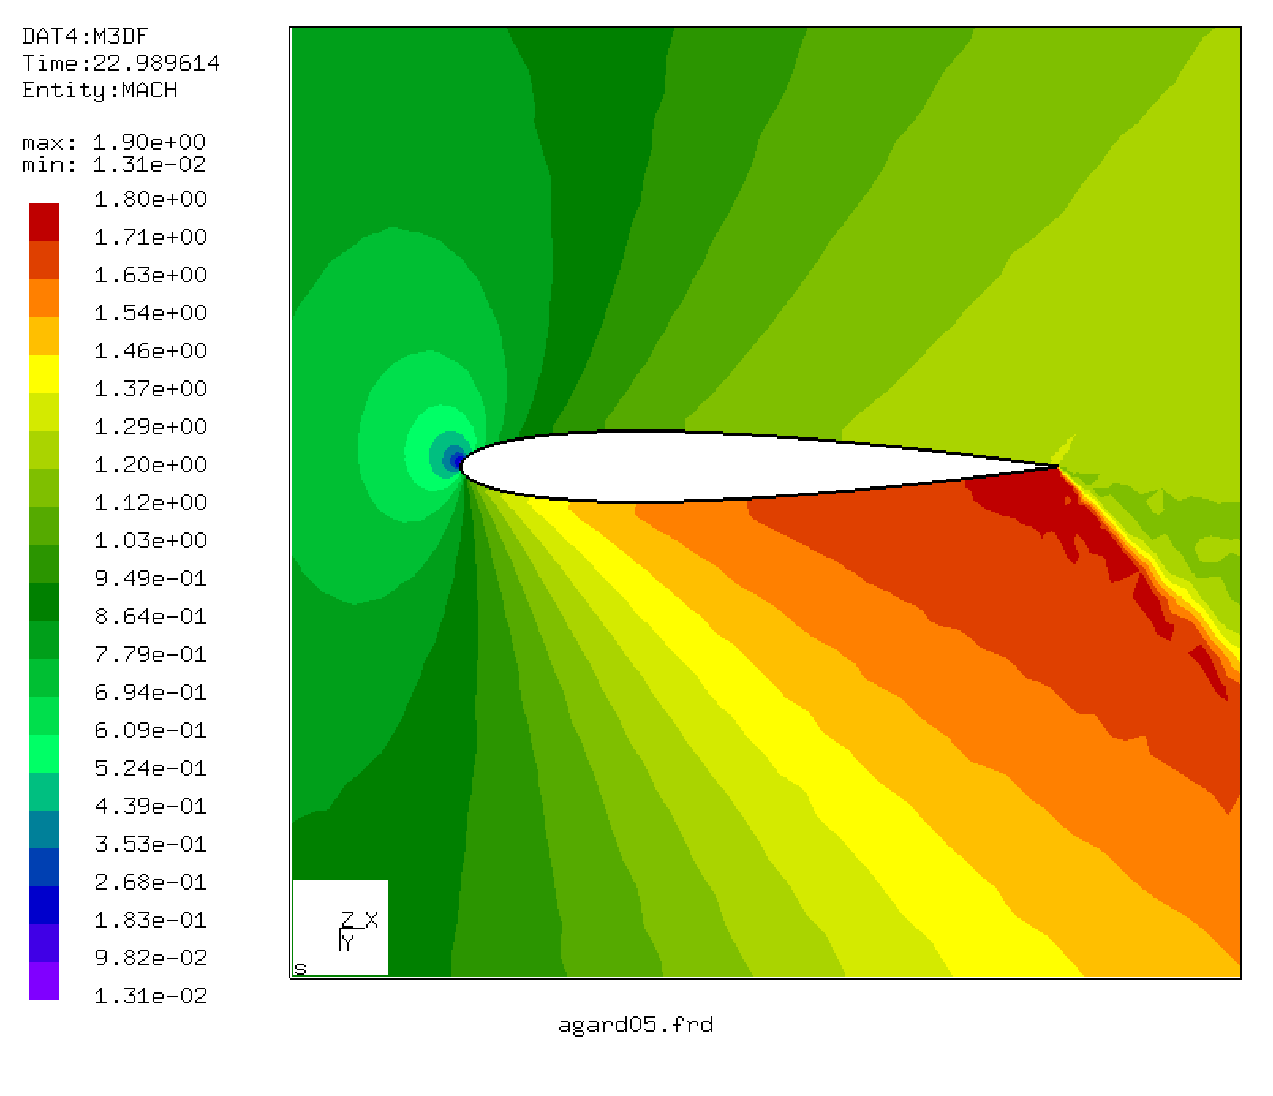
\epsfig{file=agard05_m.eps,width=9cm}
\caption{\label{naca012m}Mach number in the naca012 airfoil flow}
\end{center}
\end{figure}

\begin{figure}
\begin{center}
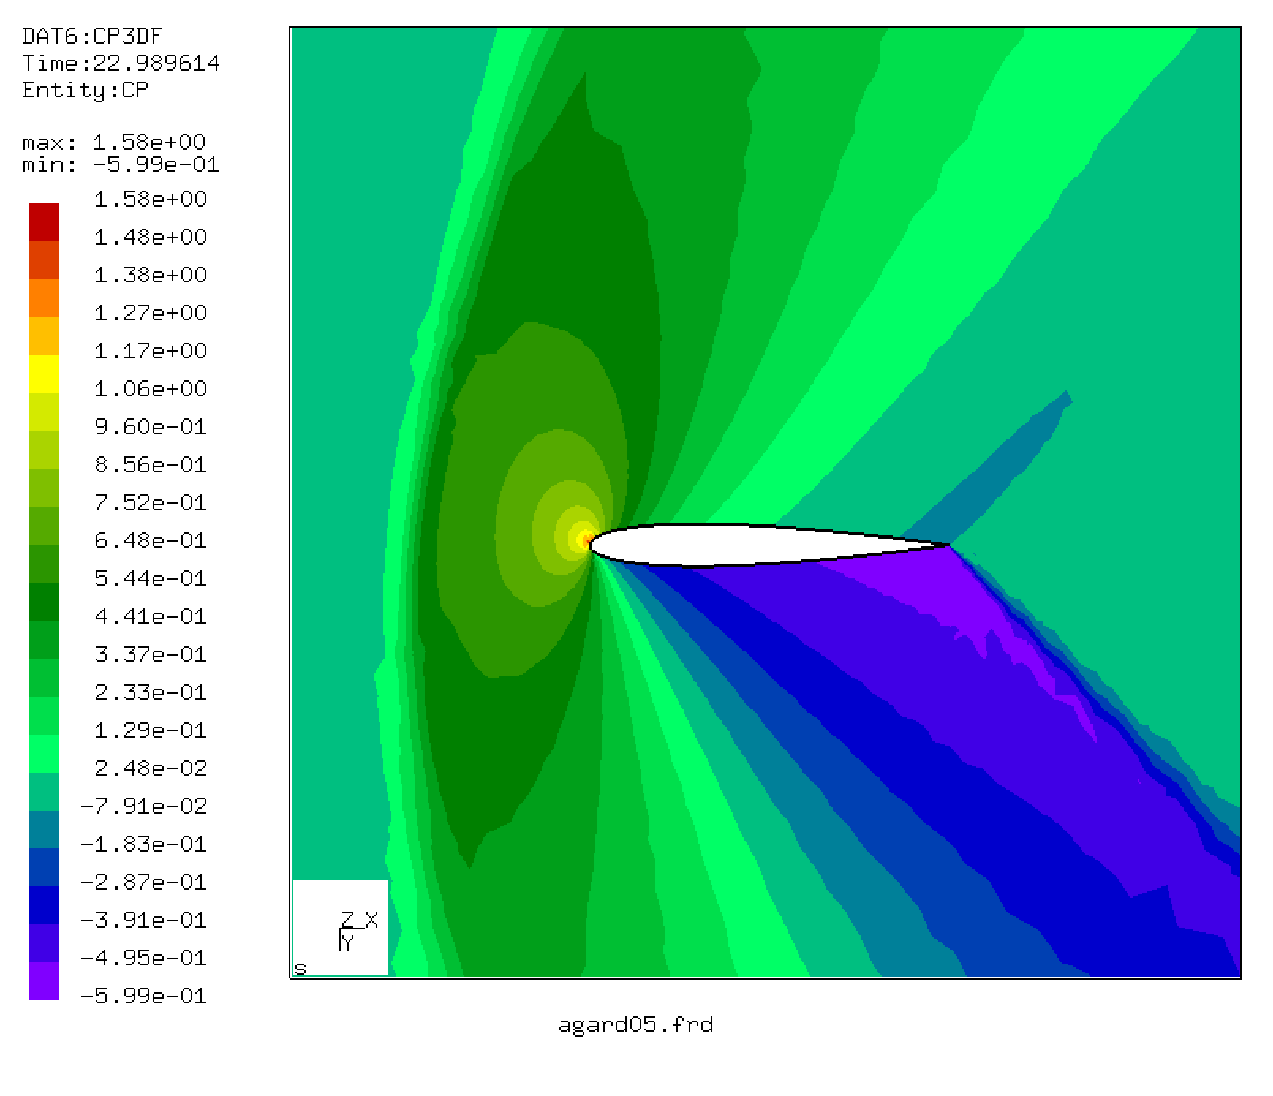
\epsfig{file=agard05_cp.eps,width=9cm}
\caption{\label{naca012cp}Pressure coefficient in the naca012 airfoil flow}
\end{center}
\end{figure}

In \cite{Pulliam} the results of CFD-calculations for several airfoils are
reported. Here, the computations for $M_\infty = 1.2$ (Mach number at infinity)
and $\alpha=7.$ (angle of attack) are reported. The input deck for this
calculation can be found in the fluid examples test suite for the Finite
Element Method (agard05.inp).

To explain the differences in the input deck between incompressible and
compressible flow the crucial section from the compressible input deck is
reproduced below.

\begin{verbatim}
*EQUATION
2
3,2,-0.99030509E+00,3,1,-0.13890940E+00
2
3756,2,-0.99030509E+00,3756,1,-0.13890940E+00
...
*MATERIAL,NAME=AIR
*CONDUCTIVITY
0.
*FLUID CONSTANTS
1.,0.,293.
*SPECIFIC GAS CONSTANT
0.285714286d0
*SOLID SECTION,ELSET=Eall,MATERIAL=AIR
*PHYSICAL CONSTANTS,ABSOLUTE ZERO=0.
*INITIAL CONDITIONS,TYPE=FLUID VELOCITY
Nall,1,0.99254615
Nall,2,0.12186934
Nall,3,0.d0
*INITIAL CONDITIONS,TYPE=PRESSURE
Nall,0.49603175
*INITIAL CONDITIONS,TYPE=TEMPERATURE
Nall,1.73611111
*VALUES AT INFINITY
1.73611111,1.,0.49603175,1.,1.
**
*STEP,INCF=200000,SHOCK SMOOTHING=0.01
*CFD,STEADY STATE,COMPRESSIBLE
1.,1.
*BOUNDARY
BOU1,11,11,1.73611111
BOU1,1,1,0.99254615
BOU1,2,2,0.12186934
BOU1,8,8,0.49603175
Nall,3,3,0.
*NODE FILE,FREQUENCYF=40000
VF,PSF,CP,TSF,TTF,MACH
*END STEP
\end{verbatim}

Since for compressible flow the temperature, velocity and pressure are linked
through the ideal gas equation, the energy conservation equation is always
used and the definition of the thermal conductivity and
specific heat is mandatory. Inviscid flow is triggered by the definition of a
zero viscosity and a zero thermal conductivity (therefore, the viscous terms
in the conservation of momentum and conservation of energy equation disappear). Slip boundary conditions at the airfoil surface are
realized through
equations. The specific gas constant is defined with the appopriate keyword. It
only depends on the kind of gas and not on the temperature. The physical
constants card is used to define absolute zero for the temperature scale. This
information is needed since the temperature in the gas equation must be specified in
Kelvin. Initial conditions must be specified for the velocity, pressure and
temperature. Careful selection of these values can shorten the computational
time. The values at infinity (defined with the \htmlref{*VALUES AT
  INFINITY}{valuesatinfinity} card) are used to calculate the pressure
coefficient $C_p = (p -p_{\inf})/(\frac{1}{2} \rho_{\inf} V_{\inf}^2)$. In
viscous calculations they can be used for the computation of the
friction coefficient too. The smoothing parameter on the *STEP card is used to
define shock smoothing and will be discussed further down.

The COMPRESSIBLE parameter on the *CFD card indicates that this is a
compressible CFD calculation. The consequence of this is that the ideal gas
equation is used to link the density, pressure and temperature. Therefore, no
*DENSITY card should be present in the input deck, and the *SPECIFIC GAS
CONSTANT card is required.
The use of the STEADY STATE parameter
tells CalculiX that the calculation is stationary. Instationary
calculations are triggered by dropping this parameter. In reality, all
CFD-calculations in CalculiX are instationary. The STEADY STATE parameter, however,
forces the calculations to be pursued until steady state is reached (so the
time used is virtual) or until the maximum number of subincrements (parameter
INCF on the *STEP card)  is reached. Transient
calculations stop as soon as the final time is reached (the time is real).

In compressible calculations shock smoothing is frequently needed in order to
avoid divergence. Shock smoothing, however, can change the
solution. Therefore, the shock smoothing coefficient, which can take values
between 0. and 2., should be chosen as small as possible. For the agard05
example a value of 0.01 was needed. In general, additional viscosity will
reduce the shock smoothing needed to avoid divergence. There is a second
effect of the shock smoothing coefficient: there is no clear steady state
convergence any more. In order to understand this some additional information
about the way CFD-calculations in CalculiX are performed is needed. The initial increment size
which is specified by the user underneath the *CFD card is a
mechanical increment size. For each mechanical increment an instationary CFD-calculation is
performed subject to the actual loads (up to steady state for a STEADY STATE
calculation). For this CFD-calculation subincrements are used, the size of
which depends on the physical characteristics of the flow (viscosity, heat
conductivity etc.). They are determined such that stability is assured (or at
least very likely). In CalculiX, steady state convergence is detected as
soon as the change in the conservative variables ($\rho, \rho u, \rho v$ etc.)
from subincrement to subincrement does not exceed $10.^{-8}$ times the actual values of these variables. In
calculations with a nonzero shock smoothing coefficient the change in
variables at first decreases down to a certain level about which it oscillates
erraticaly.  Therefore, it is likely that convergence will never be detected. The change in the conservative variables is
stored in a file with the name jobname.fcv (assuming the input deck to be jobname.inp). The user may force convergence by
limiting the number of subincrements with the INCF parameter on the *STEP
card. As soon as INCF subincrements are calculated the CFD-calculation is
assumed to be finished and the next mechanical increment is started.

The smoothing coefficient may be further reduced by choosing smaller CFD
subincrements. The fifth entry underneath the *CFD-card is the factor by which
the CFD increment size calculated based on physical parameters such as
viscosity and local velocity is divided. Default is 1.25 for compressible
calculatons and 1. for incompressible calculations. The factor cannot be
less than the default. For instance, a factor of 5. implies that the time
increment is chosen as 20 \% of the physically based time increment. Larger
factors will decrease the need for shock smoothing but also linearly increase
the computational time.

If the calculation diverges, the shock smoothing coefficient is set to 0.001
if it was zero before, and to twice its value else, and the calculation is
repeated. If the value exceeds 2 the calculation is stops with an error
message. Shock smoothing is only used for compressible calculations.

Figure \ref{naca012} shows the mesh used for the agard05 calculation. It
consists of linear wedge elements. In CalculiX, only linear elements
(tetrahedra, hexahedra or wedges) are allowed for CFD-calculations. It is
finer along the airfoil (but not as fine as needed to capture the boundary
layer in viscous calculations). Figures \ref{naca012m} and  \ref{naca012cp}
show the Mach number and the pressure coefficient, respectively. The maximum
Mach number in \cite{Pulliam} is about 1.78, the maximum pressure coefficient
is about -0.55. This agrees well with the present results. Increasing the
shock smoothing coefficient leads to smoothing fringe plots, however, the
actual values become worse.

The total temperature for this calculation (not shown here) was nearly constant. Recall that the
total change of the total temperature along a stream line is given by:

\begin{equation}
\frac{D \rho c_p T_t}{D t} = (t^{lm} v_m)_{,l} - \boldsymbol{\nabla} \cdot
\boldsymbol{q} + \rho h_{ \theta} + \frac{\partial p}{\partial t} + \rho f^m v^k
\delta_{mk}.
\end{equation}

The terms on the right hand side correspond to the viscous work (zero), the
heat flow (zero, since the heat conduction coefficient is zero), the
heat introduced per unit mass (zero), the change in pressure (zero in the
steady state regime) and the work by external body forces (zero).

\subsection{Laminar viscous compressible compression corner flow}

\begin{figure}
\begin{center}
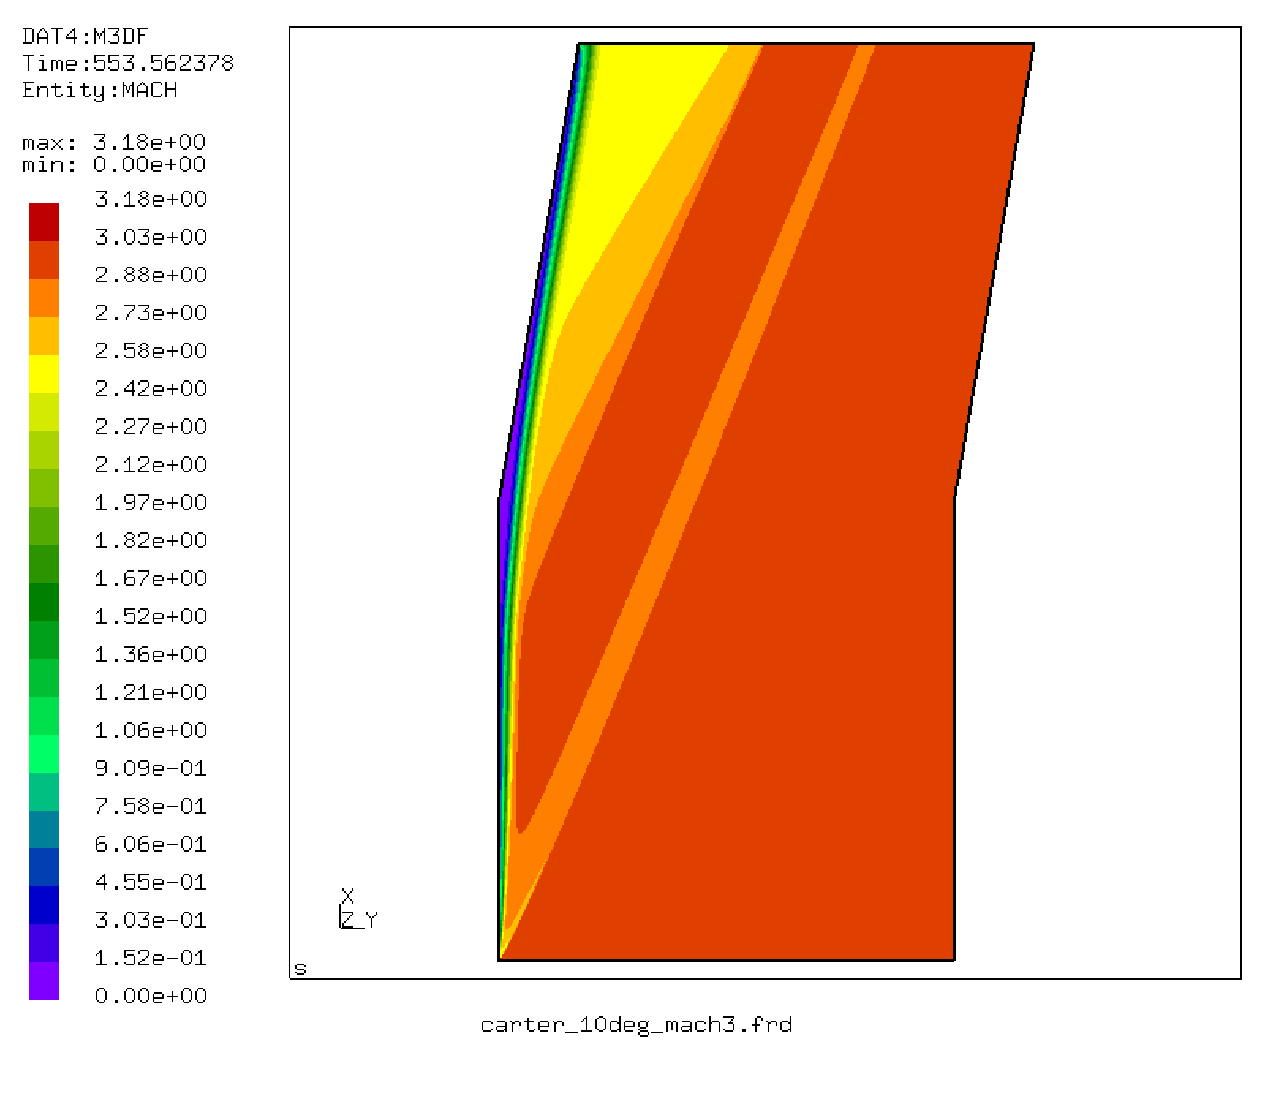
\epsfig{file=carter_m.eps,width=12cm}
\caption{\label{carterm}Mach number for the Carter problem}
\end{center}
\end{figure}

\begin{figure}
\begin{center}
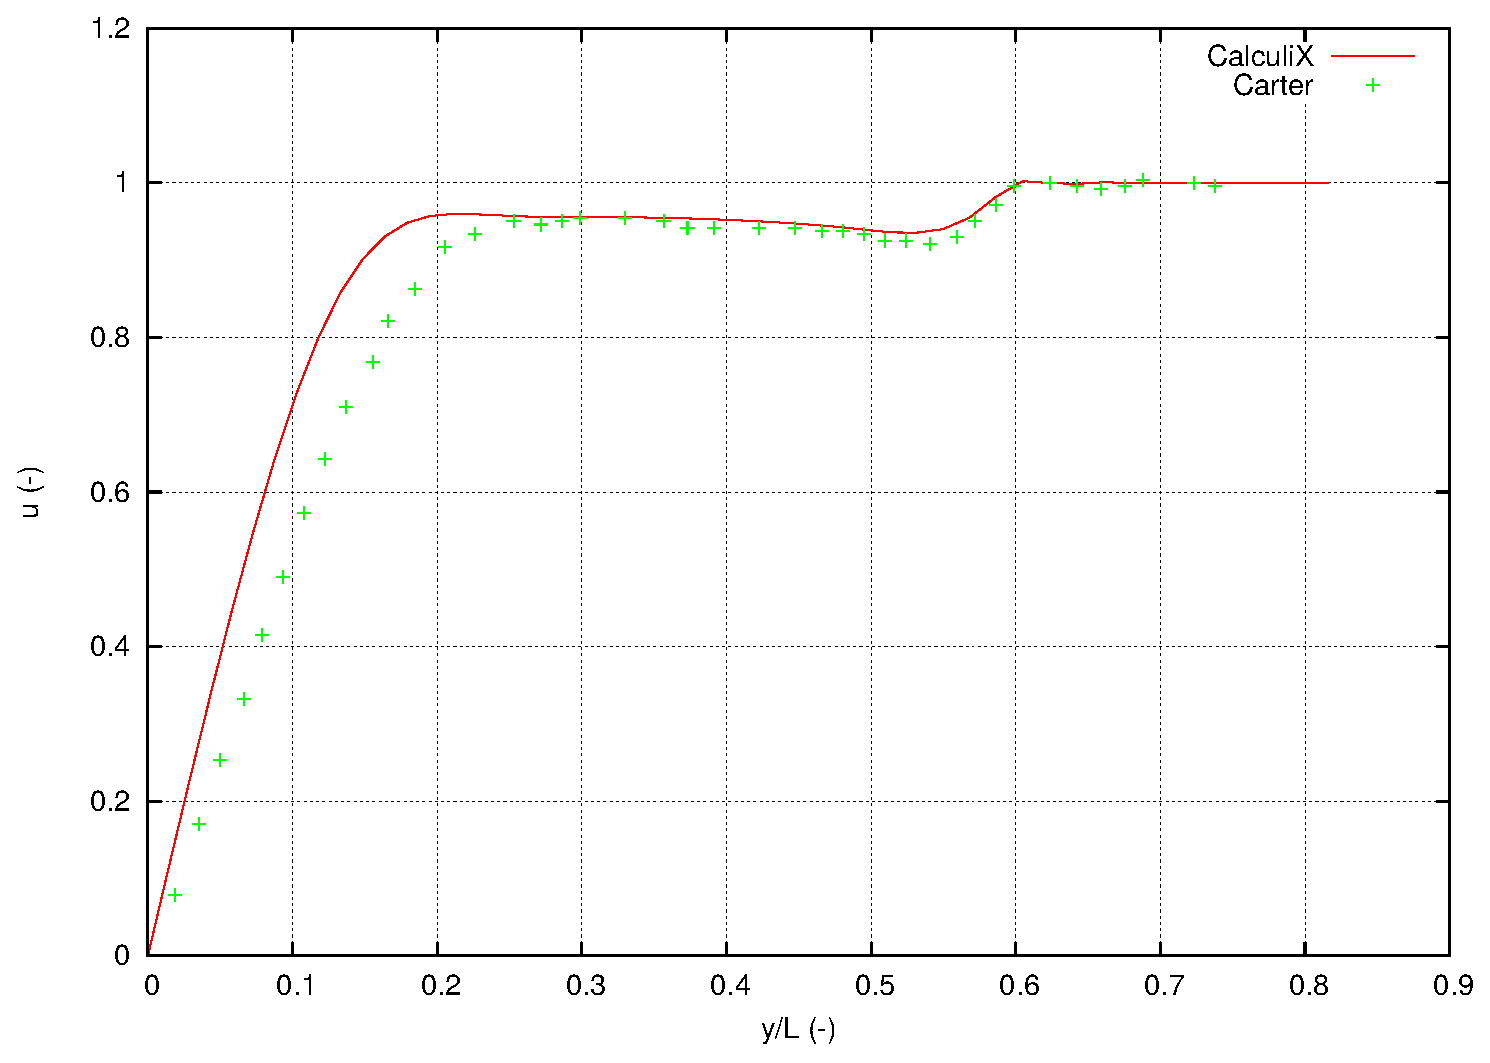
\epsfig{file=carter_u.eps,width=8cm}
\caption{\label{carteru}velocity profile across the flow for the Carter problem}
\end{center}
\end{figure}

\begin{figure}
\begin{center}
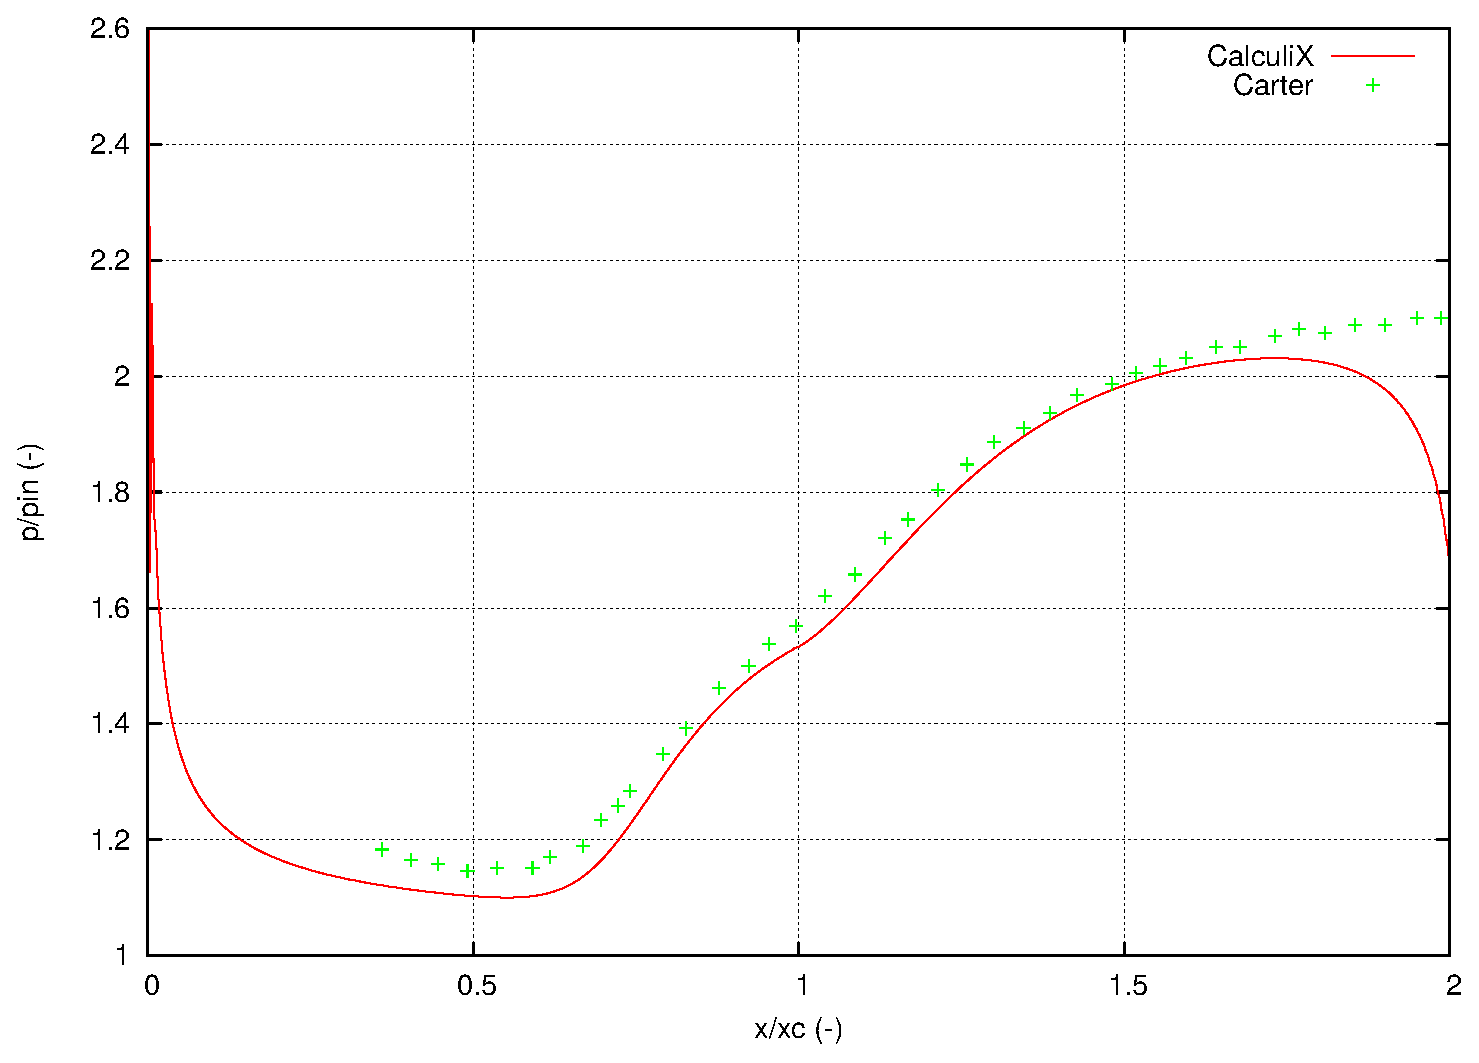
\epsfig{file=carter_p.eps,width=8cm}
\caption{\label{carterp}Static pressure at the wall for the Carter problem}
\end{center}
\end{figure}

This benchmark example is described in \cite{Carter}. The input deck for the
CalculiX computation is called carter\_10deg\_mach3.inp and can be found in the
fluid test example suite. The flow is entering at Mach 3 parallel to a plate
of length 16.8 after which a corner of $10^{\circ}$ arises. The Reynolds
number based on a unit length is 1000., which yields for a unit velocity a
dynamic viscosity coefficient $\mu=10^{-3}$. No units are specified: the user
can choose appropriate consistent units. Choosing $c_p=1$ and $\kappa=1.4$
leads to a specific gas constant $r=0.286$. The selected Mach number leads to
an inlet temperature of $T=0.278$. The ideal gas law yields a static inlet
pressure of $p=0.0794$ (assuming an unit inlet density). The wall is assumed to be isothermal at a total
temperature of $T_t=0.778$. Finally, the assumed Prandl number (Pr=$\mu c_p/\lambda$) of 0.72 leads to
a conduction coefficient of 0.00139.

A very fine mesh with about 425,000 nodes was generated, gradually finer towards
the wall ($y^+=0.885$ for the
closest node near the wall at L=1 from
the inlet, where $y^+=u_{\tau}y/\nu$ and $u_{\tau}=\sqrt{\tau/\rho}$; $y$ is
the distance from the wall and $\tau$ is the shear stress parallel to the wall ). The Mach number is shown in Figure \ref{carterm}. The shock wave
emanating from the front of the plate and the separation and reattachment
compression fan at the kink in the plate are cleary visible. One also observes
the thickening of the boundary layer near the kink leading to a recirculation
zone. Figure \ref{carteru} shows the velocity component parallel to the inlet
plate orientation across a line perpendicular to a plate at unit length from
the entrance. One notices that the boundary layer in the CalculiX calculation
is smaller than in the Carter solution. This is caused by the
temperature-independent viscosity. Applying the Sutherland viscosity law leads
to the same boundary layer thickness as in the reference. In CalculiX, no additional shock smoothing was necessary. Figure
\ref{carterp} plots the static pressure at the wall relative to the inlet
pressure versus a normalized plate length. The reference length for the
normalization was the length of the plate between inlet and kink (16.8 unit
lengths). So the normalized length of 1 corresponds to the kink. There is a
good agreement between the CalculiX and the Carter results, apart from the
outlet zone, where the outlet boundary conditions influence the CalculiX results.

\subsection{Laminar viscous compressible airfoil flow}

\begin{figure}
\begin{center}
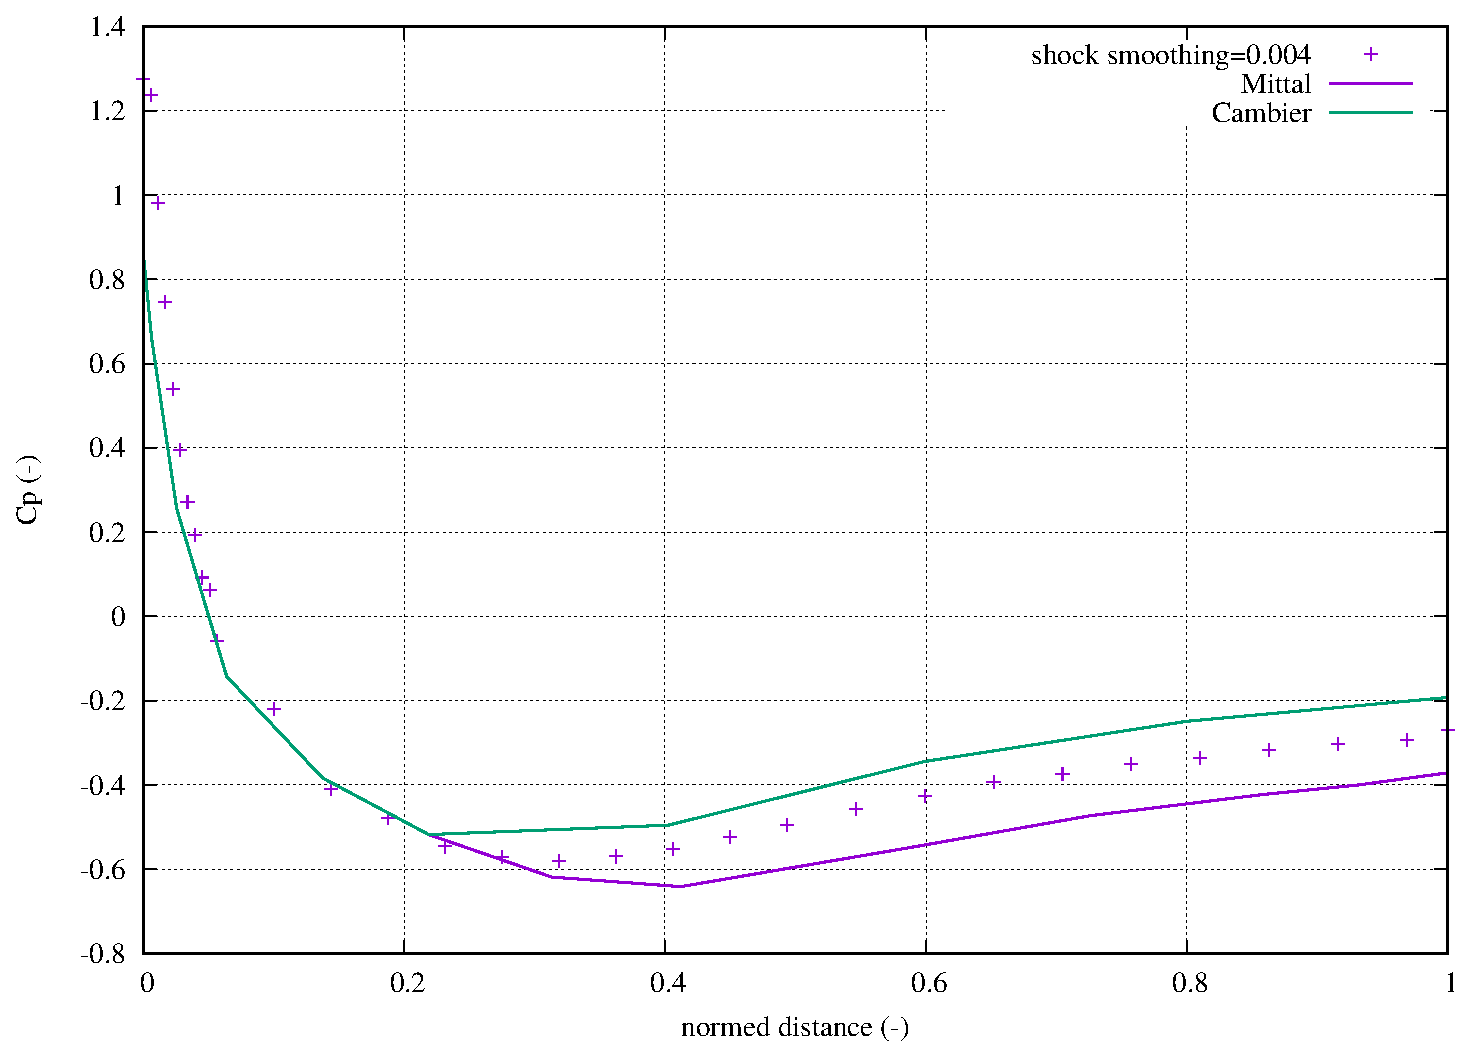
\epsfig{file=naca012_fem_cp.eps,width=8cm}
\caption{\label{nacafemcp}Pressure coefficient for laminar viscous flow about a
  naca012 airfoil}
\end{center}
\end{figure}

\begin{figure}
\begin{center}
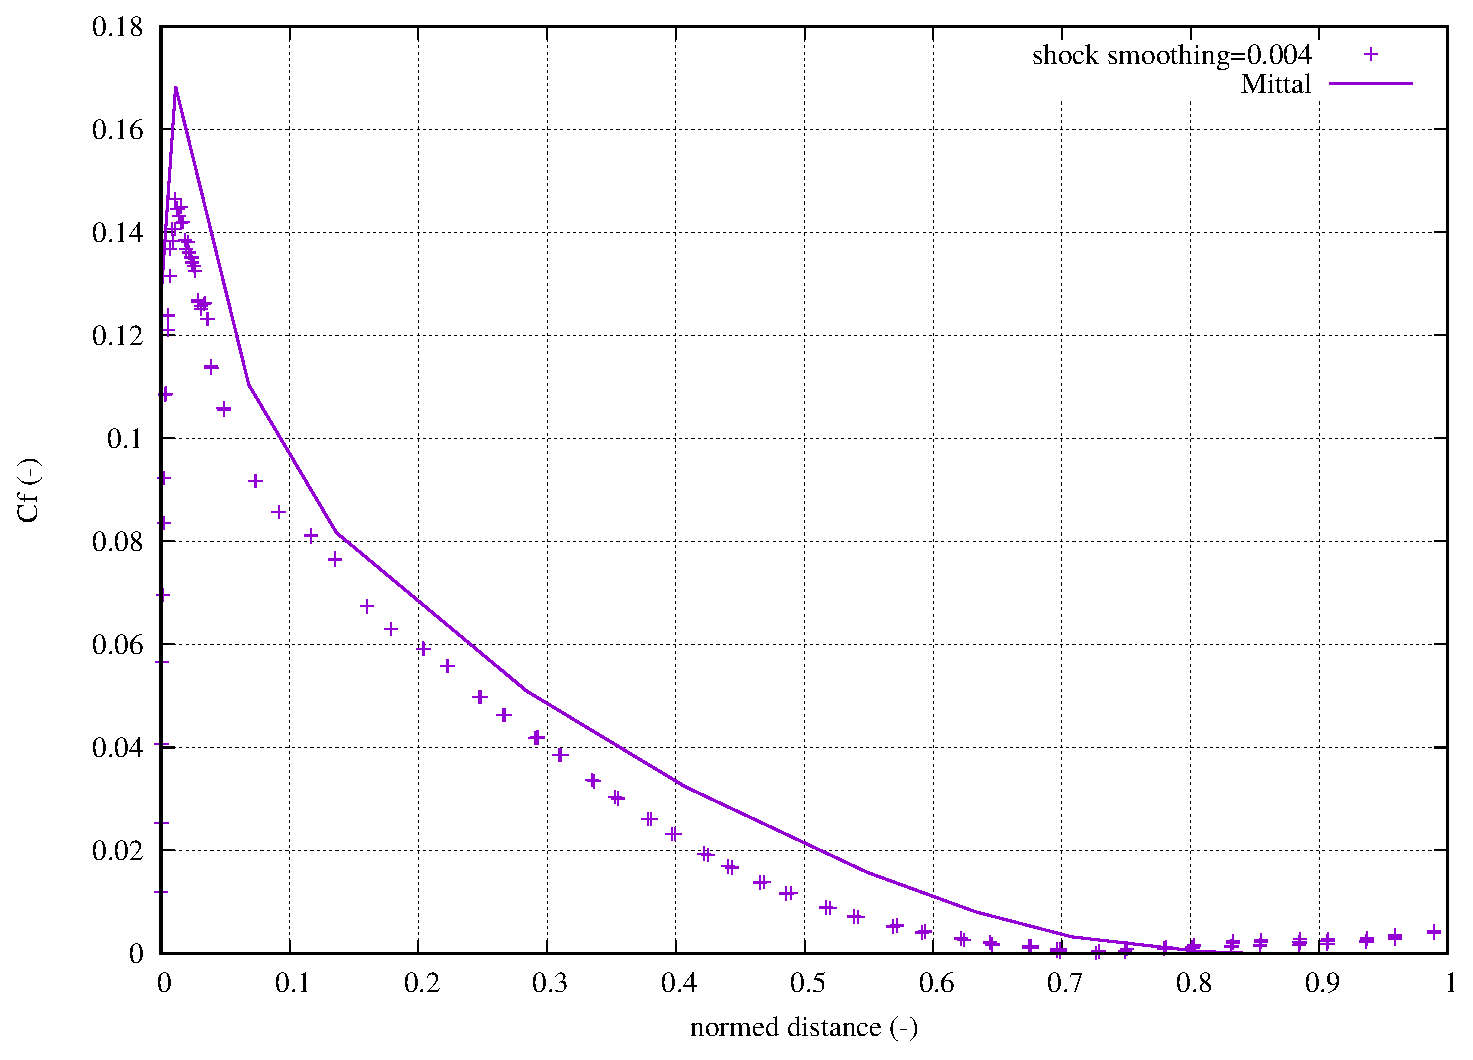
\epsfig{file=naca012_fem_cf.eps,width=8cm}
\caption{\label{nacafemcf}Friction coefficient for laminar viscous flow about a
  naca012 airfoil}
\end{center}
\end{figure}

A further example is the laminar viscous compressible flow about a naca012
airfoil. Results for this problem were reported by \cite{Mittal}. The entrance
Mach number is 0.85, the Reynolds number is 2000. Of interest is the steady
state solution. In CalculiX this is obtained by performing a transient
CFD-calculation up to steady state. The input deck for this example is called
naca012\_visc\_mach0.85.inp and can be found amoung the CFD test
examples. Basing the Reynolds number on the unity chord length of the airfoil,
a unit entrance velocity
and a unit entrance density leads to a dynamic viscosity of $\mu=5 \times
10^{-4}$. Taking $c_p=1$ and $\kappa=1.4$ leads to a specific gas constant
$r=0.2857$ (all in consistent units). Use of the entrance Mach number
determines the entrance static temperature to be $T_s=3.46$. Finally, the
ideal gas law leads to a entrance static pressure of $p_s=0.989$. Taking the
Prandl number to be 1 determines the heat conductivity $\lambda=5 \time
10^{-4}$. The surface of the airfoil is assumed to be adiabatic. 

The results for the pressure and the friction coefficient at the surface of
the airfoil are shown in Figures
\ref{nacafemcp} and \ref{nacafemcf}, respectively, as a function of the shock
smoothing coefficient. The pressure coefficient is defined by
$c_p=(p-p_\infty)/(0.5 \rho_\infty v_\infty^2)$, where p is the local static
pressure, $p_\infty$, $\rho_\infty$ and $v_\infty$ are the static pressure,
density and velocity at the entrance, respectively. Figure \ref{nacafemcp}
shows that the result for a shock smoothing coefficient of 0.004, which is the
smallest value not leading to divergence is in between the results reported by
Cambier and Mittal. The friction coefficient is defined by
$\tau_w/(0.5 \rho_\infty v_\infty^2)$, where $\tau_w$ is the local shear
stress. The CalculiX results with a shock smoothing coefficient of 0.004 are
smaller than the ones reported by Mittal. The $c_f$-peak at the front of the
airfoil is also somewhat too small: the literature result is 0.17, the CalculiX peak reaches only
up to 0.15. The shock coefficient is already very small and it is the smallest
feasible value for this mesh anyway, so decreasing the shock coefficient,
which would further increase the peak, is
not an option. A too coarse mesh density at that location may also play a role. 

\subsection{Channel with hydraulic jump}

\begin{figure}
\begin{center}
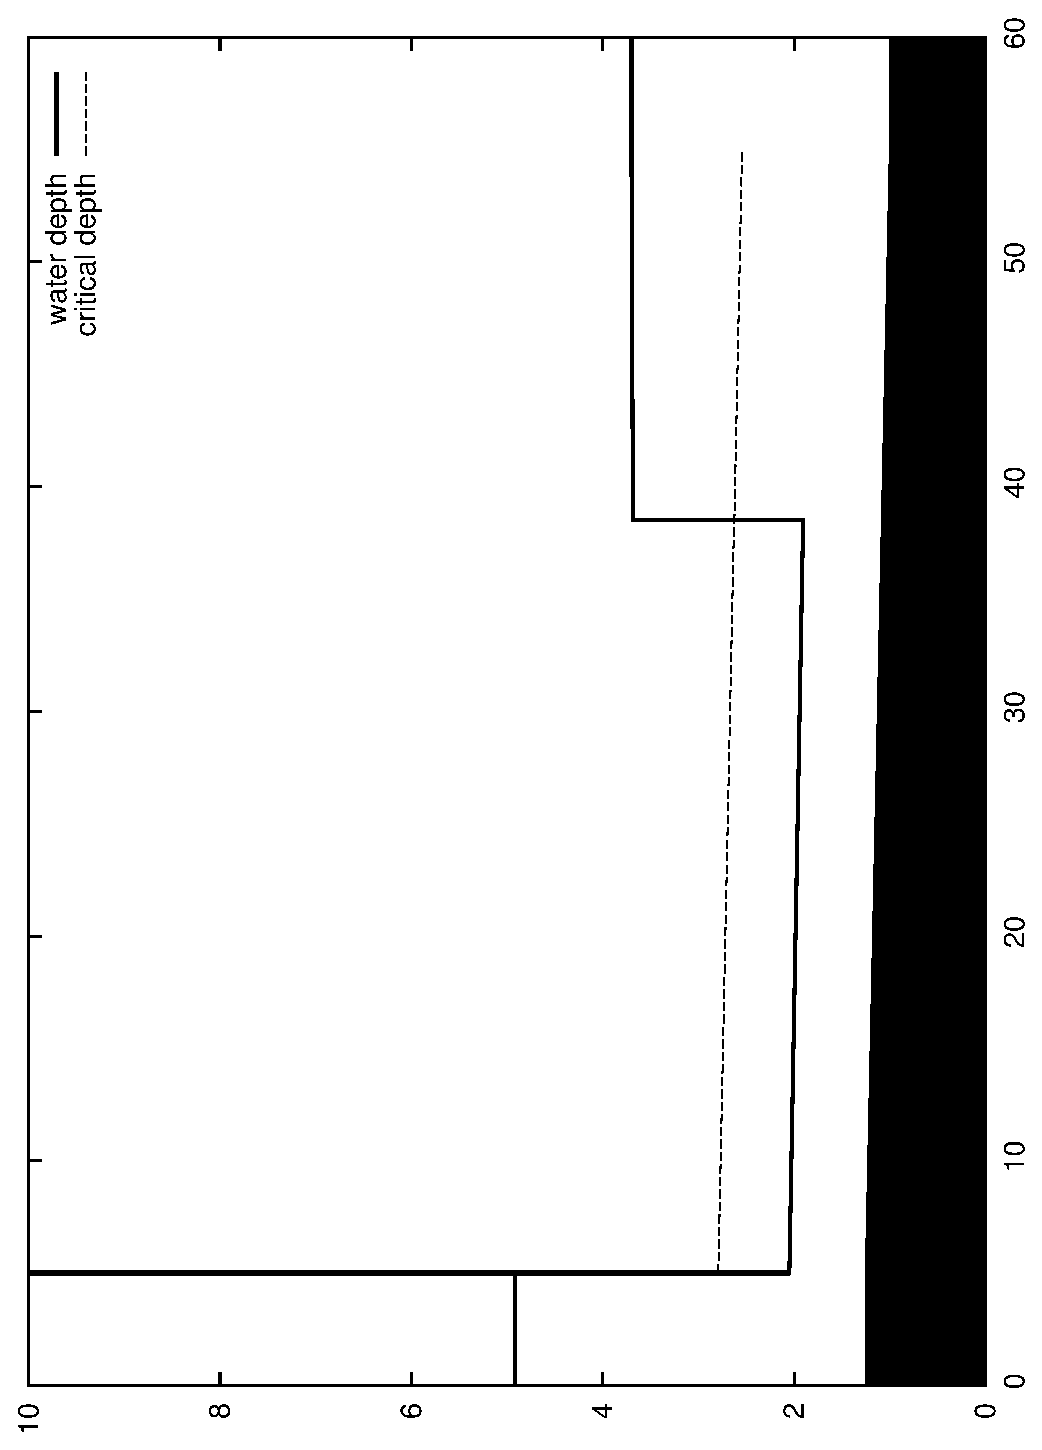
\epsfig{file=channel.eps,width=8cm,angle=-90}
\caption{\label{channel}Water depth in a channel with hydraulic jump}
\end{center}
\end{figure}

That open channel flow can be modeled as a one-dimensional network is maybe
not so well known. The governing equation is the Bresse equation
(cf. Section \ref{channels}) and the available fluid section types are
listed in Section \ref{fluidsectiontypeschannels}. 

The input deck for the present example is shown below. 

\begin{verbatim}
**
**   Structure: channel connecting two reservoirs.
**   Test objective: steep slope, frontwater - jump - 
**                   backwater curve
**
*NODE,NSET=NALL
1,0.,0.,0.
2,1.,0.,0.
4,3.,0.,0.
6,5.,0.,0.
7,6.,0.,0.
8,7.,0.,0.
9,8.,0.,0.
10,9.,0.,0.
11,10.,0.,0.
*ELEMENT,TYPE=D,ELSET=EALL
1,0,1,2
2,2,4,6
4,6,7,8
5,8,9,10
6,10,11,0
*MATERIAL,NAME=WATER
*DENSITY
1000.
*FLUID CONSTANTS
4217.,1750.E-6,273.
*ELSET,ELSET=E1
1,6
*ELSET,ELSET=E2
2
*ELSET,ELSET=E4
4
*ELSET,ELSET=E5
5
*FLUID SECTION,ELSET=E1,TYPE=CHANNEL INOUT,MATERIAL=WATER
*FLUID SECTION,ELSET=E2,TYPE=CHANNEL SLUICE GATE,MANNING,MATERIAL=WATER
10.,0.,0.1,0.005,0.01,0.8
*FLUID SECTION,ELSET=E4,TYPE=CHANNEL STRAIGHT,MANNING,MATERIAL=WATER
10.,0.,49.8,0.005,0.01
*FLUID SECTION,ELSET=E5,TYPE=CHANNEL RESERVOIR,MANNING,MATERIAL=WATER
10.,0.,0.1,0.005,0.01
*BOUNDARY
10,2,2,2.7
*BOUNDARY,MASS FLOW
1,1,1,60000.
*STEP
*HEAT TRANSFER,STEADY STATE
*DLOAD
EALL,GRAV,9.81,0.,0.,-1.
*NODE PRINT,NSET=NALL
U
*END STEP
\end{verbatim}

It
is one of the examples in the CalculiX test suite (channel3). The channel is made up of five
3-node network elements (type D) in one long line. The nodes have fictitious
coordinates. They do not enter the calculations, however, they are listed
in the .frd file. For a proper visualization with CalculiX GraphiX it may be
advantageous to use the correct coordinates. As usual in networks, the final
node of the entry and exit element have the label zero. The material is water
and is characterized by its density, heat capacity and dynamic
viscosity. Next, the elements are stored in appropriate sets (by using *ELSET)
for the sake of referencing in the \htmlref{*FLUID SECTION}{fluidsection} card. 

The structure of the channel becomes apparent when analyzing the *FLUID
SECTION cards: upstream there is a sluice gate,
downstream there is a large reservoir and both are connected by a straight
channel. The sluice gate is described by its width (10 m), a trapezoid angle
$\theta=0 $ (i.e. the cross section is rectangular) and a slope $S_0$ of 0.005. Since
the parameter MANNING has been used on the *FLUID SECTION card, the next
parameter (0.01 $m^{-1/3}s$) is the Manning coefficient. Finally, the gate
height is 0.8 m. The slope and the Manning coefficient are needed to calculate
the critical and the normal depth and should be the same as in the downstream
straight channel element. The constants for the straight channel
element can be checked in Section \ref{fluidsectiontypeschannels}. Important
here is the length of 49.8 m. The last element, the reservoir, is again a very
short element (length 0.1 m).

Next, the boundary conditions are defined: the reservoir fluid depth is 2.7 m,
whereas the mass flow is 60000 $kg/s$. Network calculations in CalculiX are a special
case of steady state heat transfer calculations, therefore the *HEAT TRANSFER,
STEADY STATE card is used. The prevailing force is gravity.

When running CalculiX a message appears that there is a hydraulic jump at
relative location 0.67 in element 4 (the straight channel element). This is
also clear in Figure \ref{channel}, where the channel has been drawn to
scale. The sluice gate is located at x=5 m, the reservoir starts at x=55 m. The
bottom of the channel is shaded black. The water level behind the gate was not
prescribed and is one of the results of the calculation: 3.667 m. The water
level at the gate is controlled by its height of 0.8 m. A frontwater curve
(i.e. a curve controlled by the upstream conditions - the gate)
develops downstream and connects to a backwater curve (i.e. a curve controlled
by the downstream conditions - the reservoir) by a hydraulic jump at a x-value
of 38.5 m. In other words, the jump connects the upstream supercritical flow
to the downstream subcritical flow. The critical depth is illustrated in the
figure by a dashed line. It is the depth for which the Froude number is 1:
critical flow.

In channel flow, the degrees of freedom for the mechanical displacements are
reserved for the mass flow, the water depth (the component in direction of the
gravity vector, not the depth orthogonal to the channel floor, since the latter
quantity is discontinuous at the location of a slope change) and the critical depth,
respectively. Therefore, the option U underneath the *NODE PRINT card will
lead to exactly this information in the .dat file. The same information can be
stored in the .frd file by selecting MF, DEPT and HCRI underneath the *NODE
FILE card.

\subsection{Cantilever beam using beam elements}

Previously, a thick cantilever beam was modeled with volume
elements. In the present section quadratic beam elements are used for a
similar exercise (Section
\ref{B32}). Beam
elements are easy to define: they consist of three nodes on a
line. Internally, they are expanded into volumetric elements. There are two
types of beam elements: B32 elements, which are expanded into C3D20 elements,
and B32R (reduced integration) elements, which are expanded into C3D20R
elements. Based on the results in the present section, the B32R element is
highly recommended. The B32 element, on the other hand, should be avoided
especially if section forces are needed.

The first cantilever beam which is looked at is 100 mm long and has a square
cross section of 2 x 2 $\text{mm}^2$. The axis of the beam is along the global
z-direction. This beam is modeled with just one element and loaded at its end
by a unit force in x-direction, Figure \ref{simplebeam1}. We are interested in
the stresses at integration point a and at node b,  the section forces at
the beam's fixed end, and the displacement in x at the free end. The location
of the integration point a is at $x=-1/\sqrt{3}$, $y=1/\sqrt{3}$ and
$z=50(1+1/\sqrt{3})$, the nodal coordinates of b are $x=-1$, $y=1$ and $z=100$
\cite{Dhondt}. The material is isotropic linear elastic with a Young's modulus of
100,000 MPa and a Poisson's ratio of 0.3.

\begin{figure}
\begin{center}
\epsfig{file=simplebeam1.eps,width=12cm}
\caption{\label{simplebeam1}Geometry of the beam}
\end{center}
\end{figure}

 The input deck for
this example is very similar to the simplebeam.inp example in the test suite:

\begin{verbatim}
**
**   Structure: cantilever beam, one element
**   Test objective: B32R elements.
**
*NODE,NSET=Nall
1, 0, 0, 0
2, 0, 0, 50
3, 0, 0, 100
*ELEMENT,TYPE=B32R,ELSET=EAll
1,1,2,3
*BOUNDARY
3,1,6
*MATERIAL,NAME=ALUM
*ELASTIC
1E7,.3
*BEAM SECTION,ELSET=EAll,MATERIAL=ALUM,SECTION=RECT
2.,2.
1.d0,0.d0,0.d0
*STEP
*STATIC
*CLOAD
1,1,1.
*EL PRINT,ELSET=Eall
S
*NODE FILE
U
*EL FILE,SECTION FORCES
S,NOE
*END STEP
\end{verbatim}

The
stresses at the integration points are obtained by a \htmlref{*EL
  PRINT}{elprint} card, the stresses at the nodes by the OUTPUT=3D option
(default) on
the \htmlref{*EL FILE}{elfile} card, whereas for the section forces the
SECTION FORCES option on the same card is used (this option is mutually
exclusive with the OUTPUT=3D option). The displacements are best obtained in
the non-expanded view, i.e. using the OUTPUT=2D option. This means that for
the present results the example had to be run twice: once with the OUTPUT=3D
option and once with the SECTION FORCES option.

The results are summarized in Table \ref{squarebend1}. The $\{\text{mm}, \text{N},
\text{s}, \text{K} \}$ system is used. The reference results are analytical
results using simple beam theory \cite{Popov}. The agreement is
overwhelming. The stresses at the integration points match exactly, so do the
extrapolated normal stresses to the nodes. The shear stresses need special
attention. For a beam the shear stress varies parabolically across the
section. A quadratic volumetric element can simulate only a linear stress
variation across the section. Therefore, the parabolic variation is
approximated by a constant shear stress across the section. Since the
reduced integration points (at $\pm 1/\sqrt{3}$) happen to be points at which the parabolic stress
variation attains its mean value the values at the integration points are
exact! The extrapolated values to the nodes take the same constant value and
are naturally wrong since the exact value at the corners is zero. 

The section forces are obtained by 
\begin{enumerate}
\item calculating the stresses at the integration points (inside the element,
  such as integration point a)
\item extrapolating those stresses to the corner nodes (such as node b)
\item calculating the stresses at the middle nodes by interpolation between
  the adjacent corner nodes
\item interpolating the stresses at all nodes within a section face onto the
  reduced integration points within the face (such as integration point c, using the shape functions of the face)
\item integrating these stresses numerically.
\end{enumerate}

As shown by Table \ref{squarebend1} this procedure yields the correct section
forces for the square beam. 

The displacements at the beam tip are off by 10 \%. The deformation of a beam
subject to a shear force at its end is third order, however, the C3D20R
element can only simulate a quadratic behavior. The deviation is reduced to
2.4 \% by using 5 elements (Table \ref{squarebend5}). Notice that integration
point a is now closer to the fixation (same position is before but in the
element adjacent to the fixation).

\begin{table}
\caption{Results for the square section beam subject to bending (1 element).\label{squarebend1}}
\begin{center}
\begin{tabular}{|c|c|c|}
\hline
 result  & value & reference \\
\hline
$\sigma_{zz}(a)$ & 34.151  & 34.151 \\
$\sigma_{xz}(a)$ & -0.25  & -0.25 \\
$F_{xx}$ & -1.  & -1. \\
$M_{yy}$ & 100.  & 100. \\
$\sigma_{zz}(b)$ & 75.  & 75. \\
$\sigma_{xz}(b)$ & -0.25  & 0. \\
$u_{x}$ & 2.25  & 2.50 \\
\hline
\end{tabular}
\end{center}        
\end{table}

\begin{table}
\caption{Results for the square section beam subject to bending (5 elements).\label{squarebend5}}
\begin{center}
\begin{tabular}{|c|c|c|}
\hline
 result  & value & reference \\
\hline
$\sigma_{zz}(a)$ & 41.471  & 41.471 \\
$\sigma_{xz}(a)$ & -0.25  & -0.25 \\
$F_{xx}$ & -1.  & -1. \\
$M_{yy}$ & 100.  & 100. \\
$\sigma_{zz}(b)$ & 75.  & 75. \\
$\sigma_{xz}(b)$ & -0.25  & 0. \\
$u_{x}$ & 2.44  & 2.50 \\
\hline
\end{tabular}
\end{center}        
\end{table}

The same beam was now subjected to a torque of 1 Nmm at its free end. The
results are summarized in Table \ref{squaretorque1}.

\begin{table}
\caption{Results for the square section beam subject to torsion (1 element).\label{squaretorque1}}
\begin{center}
\begin{tabular}{|c|c|c|}
\hline
 result  & value & reference \\
\hline
$\sigma_{xz}(a)$ & -0.21651  & - \\
$\sigma_{yz}(a)$ & -0.21651  & - \\
$M_{zz}$ & 1.  & 1. \\
$\sigma_{xz}(b)$ & -0.375  & 0 \\
$\sigma_{yz}(b)$ & -0.375  & 0 \\
$u_{y}$ & $9.75 \cdot 10^{-4}$  & $1.1525 \cdot 10^{-3}$ \\
\hline
\end{tabular}
\end{center}        
\end{table}

The torque is matched perfectly, the torsion at the end of the beam ($u_y$ is
the displacement in y-direction at the corresponding node of node b) is off by
15 \% \cite{Popov}. The shear stresses at node b are definitely not correct
(there is no shear stress at a corner node), however, the integration of the
values interpolated from the nodes at the facial integration points yields the
exact torque! Using more elements does not change the values in Table
\ref{squaretorque1}. 

The same exercise is now repeated for a circular cross section (radius = 1 mm,
same length, boundary conditions and material data as for the rectangular
cross section). For such a
cross section the vertex nodes of the element lie at $x,y = \pm 0.7071, \pm 0.7071 $,
whereas the middle nodes lie at $x,y = 0,\pm 1$ and $x,y = \pm 1,0$. The
integration points are located at $x,y = \pm 0.5210 $. The results for bending
with just one element are shown in Table \ref{circbend1} and with 5 elements
in Table  \ref{circbend5}.

\begin{table}
\caption{Results for the circular section beam subject to bending (1 element).\label{circbend1}}
\begin{center}
\begin{tabular}{|c|c|c|}
\hline
 result  & value & reference \\
\hline
$\sigma_{zz}(a)$ & 34.00  & 52.26 \\
$\sigma_{xz}(a)$ & -0.322  & -0.318 \\
$F_{xx}$ & -0.99996  & -1. \\
$M_{yy}$ & 58.7  & 100. \\
$\sigma_{zz}(b)$ & 62.8  & 90.03 \\
$\sigma_{xz}(b)$ & -0.322  & -0.318 \\
$u_{x}$ & 2.91  & 4.24 \\
\hline
\end{tabular}
\end{center}        
\end{table}

\begin{table}
\caption{Results for the circular section beam subject to bending (5 elements).\label{circbend5}}
\begin{center}
\begin{tabular}{|c|c|c|}
\hline
 result  & value & reference \\
\hline
$\sigma_{zz}(a)$ & 59.77  & 63.41 \\
$\sigma_{xz}(a)$ & -0.322  & -0.318 \\
$F_{xx}$ & -0.99996  & -1. \\
$M_{yy}$ & 102.  & 100. \\
$\sigma_{zz}(b)$ & 109.  & 90.03 \\
$\sigma_{xz}(b)$ & -0.322  & -0.318 \\
$u_{x}$ & 3.86  & 4.24 \\
\hline
\end{tabular}
\end{center}        
\end{table}

For just one element the shear stress is quite close to the analytical value,
leading to a even better match of the shear force. This is remarkable an can
only be explained by the fact that the cross area of the piecewise quadratic
approximation of the circular circumference is smaller and exactly compensates
the slightly higher shear stress. A similar effect will be noticed for the
torque. The normal stress, however, is far off at the integration points as
well as at the nodes leading to a bending moment which is way too small. The
same applies to the deformation in x-direction. Using five elements leads to a
significant improvement: the bending moment is only 2 \% off, the deformation
at the free end 9 \%. Here again one can argue that the deformation is of
cubic order, whereas a quadratic element can only  simulate a quadratic
change. Using more elements consequently improves the results.

The results for a torque applied to a circular cross section beam is shown in
Table \ref{circtorque1} (1 element; the results for 5 elements are identical).

\begin{table}
\caption{Results for the circular section beam subject to torsion (1 element).\label{circtorque1}}
\begin{center}
\begin{tabular}{|c|c|c|}
\hline
 result  & value & reference \\
\hline
$\sigma_{xz}(a)$ & -0.309  & -0.331 \\
$\sigma_{yz}(a)$ & -0.309  & -0.331 \\
$M_{zz}$ & 0.999994  & 1. \\
$\sigma_{xz}(b)$ & -0.535  & -0.450 \\
$\sigma_{yz}(b)$ & -0.535  & -0.450 \\
$u_{y}$ & $1.54 \cdot 10^{-3}$  & $1.66 \cdot 10^{-3}$ \\
\hline
\end{tabular}
\end{center}        
\end{table}

Again, it is remarkable that the torque is perfectly matched, although the
shear stress at the integration points is 6 \% off. This leads to shear values
at the vertex nodes which are 19 \% off. Interpolation to the facial
integration points yields shear stresses of -0.305 MPa. Integration of these
stresses finally leads to the perfect torque values. The torsion angle at the
end of the beam is 7 \%off. 

Summarizing, one can state that the use of C3D20R elements leads to quite
remarkable results:

\begin{itemize}
\item For a rectangular cross section:
\begin{itemize}
\item the section forces are correct
\item the stresses at the integration points are correct
\item the displacements for bending are correct, provided enough elements are
  used
\item the torsion angle is somewhat off (15 \%).
\end{itemize}
\item For a circular cross section:
\begin{itemize}
\item the shear force and torque section forces are correct
\item the bending moment is correct if enough elements are used
\item the displacements for bending are correct, provided enough elements are used
\item the torsion angle is somewhat off (7 \%).
\end{itemize}
\end{itemize}

It is generally recommended to calculate the stresses from the section
forces. 
 The only drawback is the C3D20R element may lead to
hourglassing, leading to weird displacements. However, the mean of the
displacements across the cross section is usually fine. An additional problem which
can arise is that nonlinear geometric calculations may not converge due to this
hourglassing. This is remedied in CalculiX by slightly perturbing the
coordinates of the expanded nodes (by about 0.1 \%).

A similar exercise was performed for the B32 element, however, the results
were quite discouraging. The section forces were, especially for bending, way
off. 

\subsection{Reinforced concrete cantilever beam}

Purpose of this exercise is to calculate the stresses in a reinforced concrete cantilever
beam due to its own weight. Special issues in this type of problem are the
treatment of the structure as a composite and the presence of a
compression-only material (the concrete). 

The input deck runs like:

\begin{verbatim}
*NODE, NSET=Nall
       1,1.000000000000e+01,0.000000000000e+00,0.000000000000e+00
...
*ELEMENT, TYPE=S8R, ELSET=Eall
     1,      1,      2,      3,      4,      5,      6,      7,      8
     2,      2,      9,     10,      3,     11,     12,     13,      6
...
** Names based on left
*NSET,NSET=Nleft 
49, 
50, 
52, 
** Names based on right
*NSET,NSET=Nright 
1, 
4, 
8, 
*MATERIAL,NAME=COMPRESSION_ONLY
*USER MATERIAL,CONSTANTS=2
  1.4e10,        1.e5
*DENSITY
2350.
*MATERIAL,NAME=STEEL
*ELASTIC
210000.e6,.3
*DENSITY
7800.
*SHELL SECTION,ELSET=Eall,COMPOSITE
.09,,COMPRESSION_ONLY
.01,,STEEL
.1,,COMPRESSION_ONLY
.1,,COMPRESSION_ONLY
.1,,COMPRESSION_ONLY
.1,,COMPRESSION_ONLY
.1,,COMPRESSION_ONLY
.1,,COMPRESSION_ONLY
.1,,COMPRESSION_ONLY
.1,,COMPRESSION_ONLY
.1,,COMPRESSION_ONLY
*BOUNDARY
Nleft,1,6
*STEP,NLGEOM
*STATIC
1.,1.
*DLOAD
Eall,GRAV,9.81,0.,0.,-1.
*NODE FILE
U
*EL FILE
S
*END STEP
\end{verbatim}

The beam has a cross section of 1 x 1 $\text{m}^2$ and a length of 10 m. The
density of concrete is 2350 $\text{kg}/\text{m}^3$, whereas the density of
steel is 7800 $\text{kg}/\text{m}^3$. The
Young's moduli are 14000 MPa and 210000 MPa, respectively. Steel is
provided only on the top of the beam (tension side of the beam) at a distance
of 9.5 cm from the upper surface. Its layer thickness is 1 cm (in reality the
steel is placed within the concrete in the form of bars. The modeling as a
thin layer is an approximation. One has to make sure that the complete section
of the bars equals the section of the layer). 
Using the composite feature
available for shell structures significantly simplifies the input. Notice that
this feature is not (yet) available for beam elements. Consequently the beam
was modeled as a plate with a width of 1 m and a length of 10
m. Underneath the *SHELL SECTION card the thickness of the layers and their
material is listed, starting at the top of the beam. The direction (from top
to bottom) is controlled by the direction of the normal on the shell elements
(which is controlled by the order in which the elements' nodes are listed
underneath the *ELEMENT card). In a composite shell there are two integration
points across each layer. Use of the S8R element or S6 element is mandatory. In order to
capture the location of the neutral axis several layers were used to model the
concrete part of the section (in total 10 layers for the concrete and 1 for
the steel). 

Concrete cannot sustain tension whereas it is largely linear elastic under
pressure. This can be modeled with the COMPRESSION\_ONLY material model. In
CalculiX this is an example of a user material. The name of user materials has
to start with a fixed character set, in this case ''COMPRESSION\_ONLY''. The
remaining 64 characters (a material name can be at most 80 characters long)
can be freely chosen. In the present input deck no extra characters were
selected. Choosing extra characters is needed if more than 1 compression-only
material is present (in order to distinguish them). The ''COMPRESSION\_ONLY''
material is characterized by 2 constants, the first is Young's modulus, the
second is the maximum tensile stress the user is willing to allow, in our case
0.1 MPa (SI-units are used).

\begin{figure}
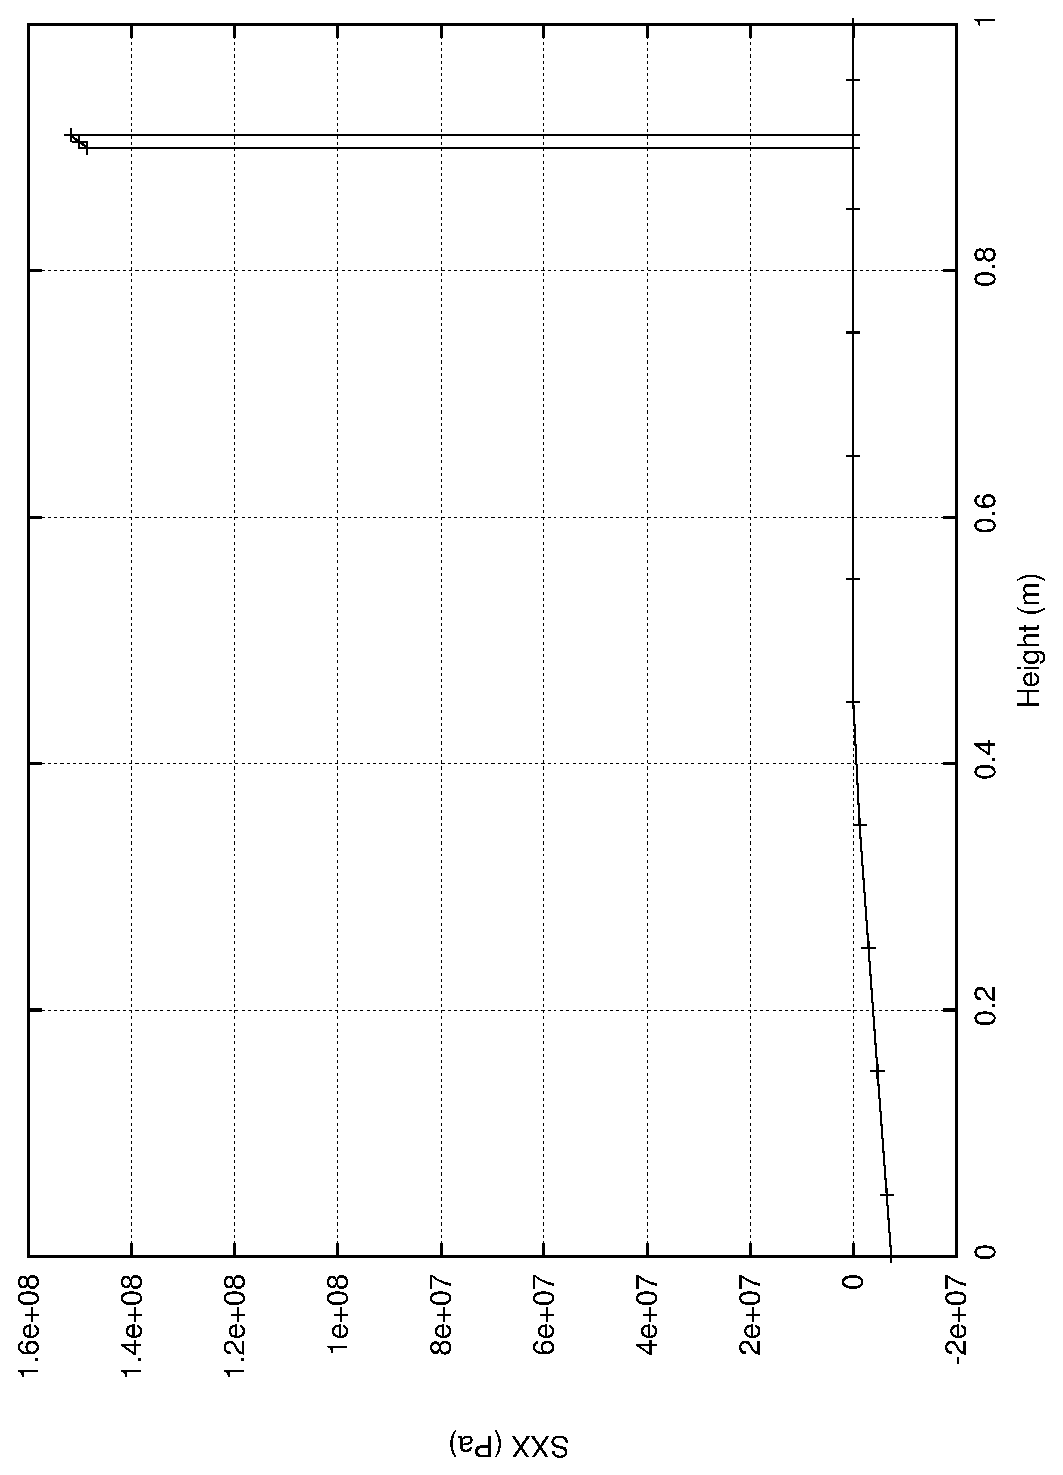
\epsfig{file=concretebeam1.eps,width=8cm,angle=270}
\caption{\label{concretebeam1}Axial stress across the height of the beam at
  the fixed end}
\end{figure}

\begin{figure}
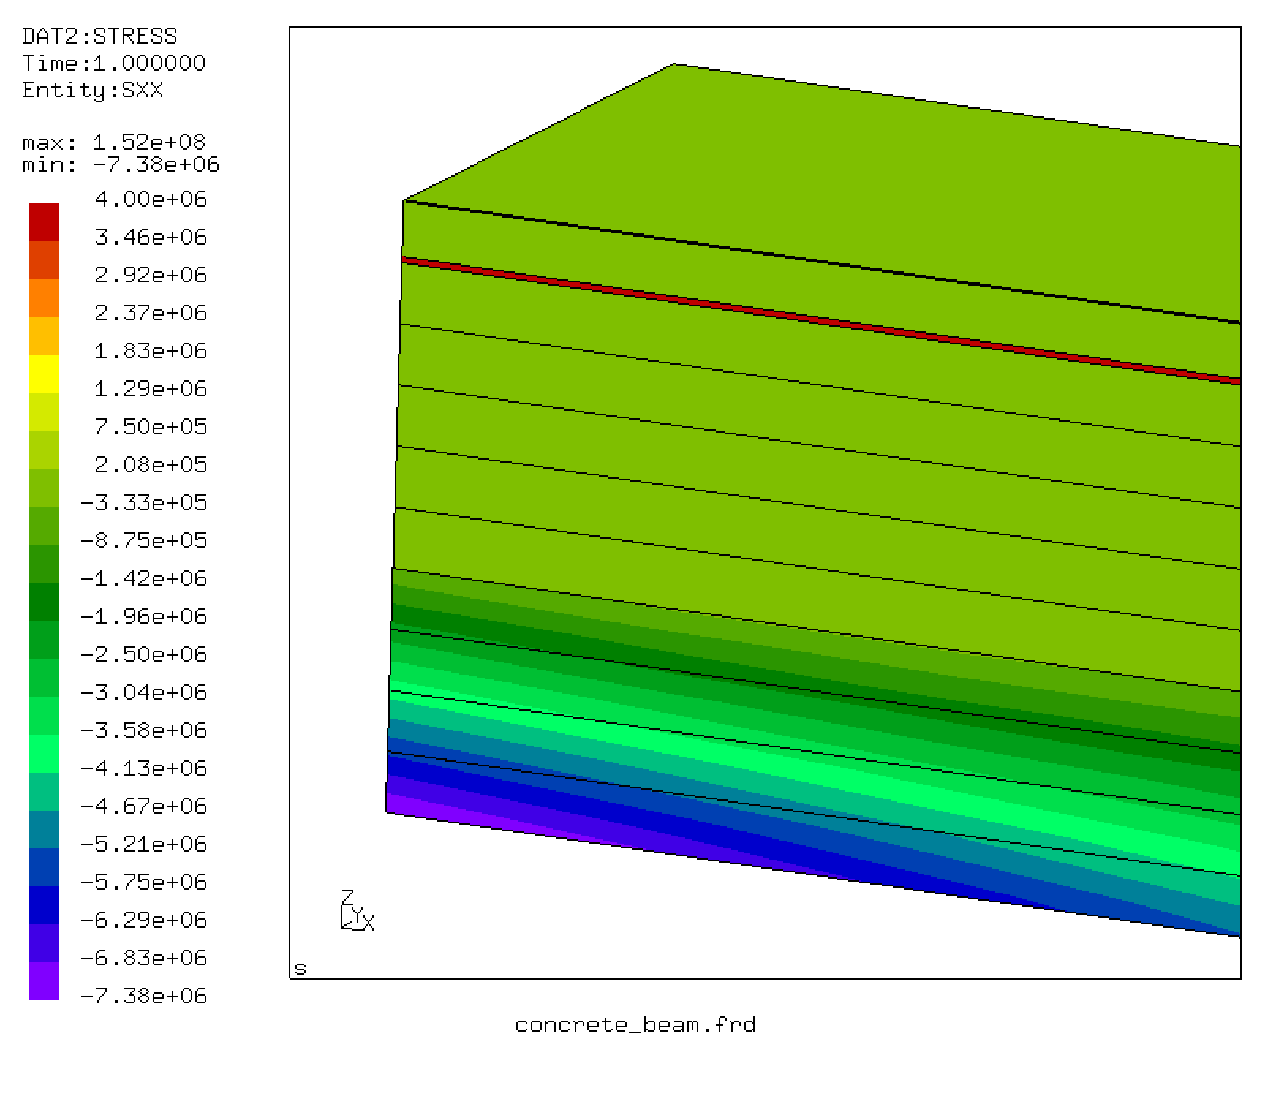
\epsfig{file=concretebeam2.eps,width=10cm}
\caption{\label{concretebeam2}Axial stress across the height of the beam at
  the fixed end}
\end{figure}

Using simple beam theory (\cite{Mortelmans}) leads to a tensile stress of
152.3 MPa in the steel and a maximum compressive stress of 7.77 MPa at
the lower edge of the concrete. The finite element calculation (Figure
\ref{concretebeam1}) predicts 152
MPa and 7.38 MPa, respectively, which is quite close. In CalculiX,
the graphical output of composite structures is always expanded into three
dimensions. In Figure \ref{concretebeam2} one notices the correct dimension of
the composite and the high tensile stresses in the thin steel layer. 

\subsection{Wrinkling of a thin sheet}

\begin{figure}
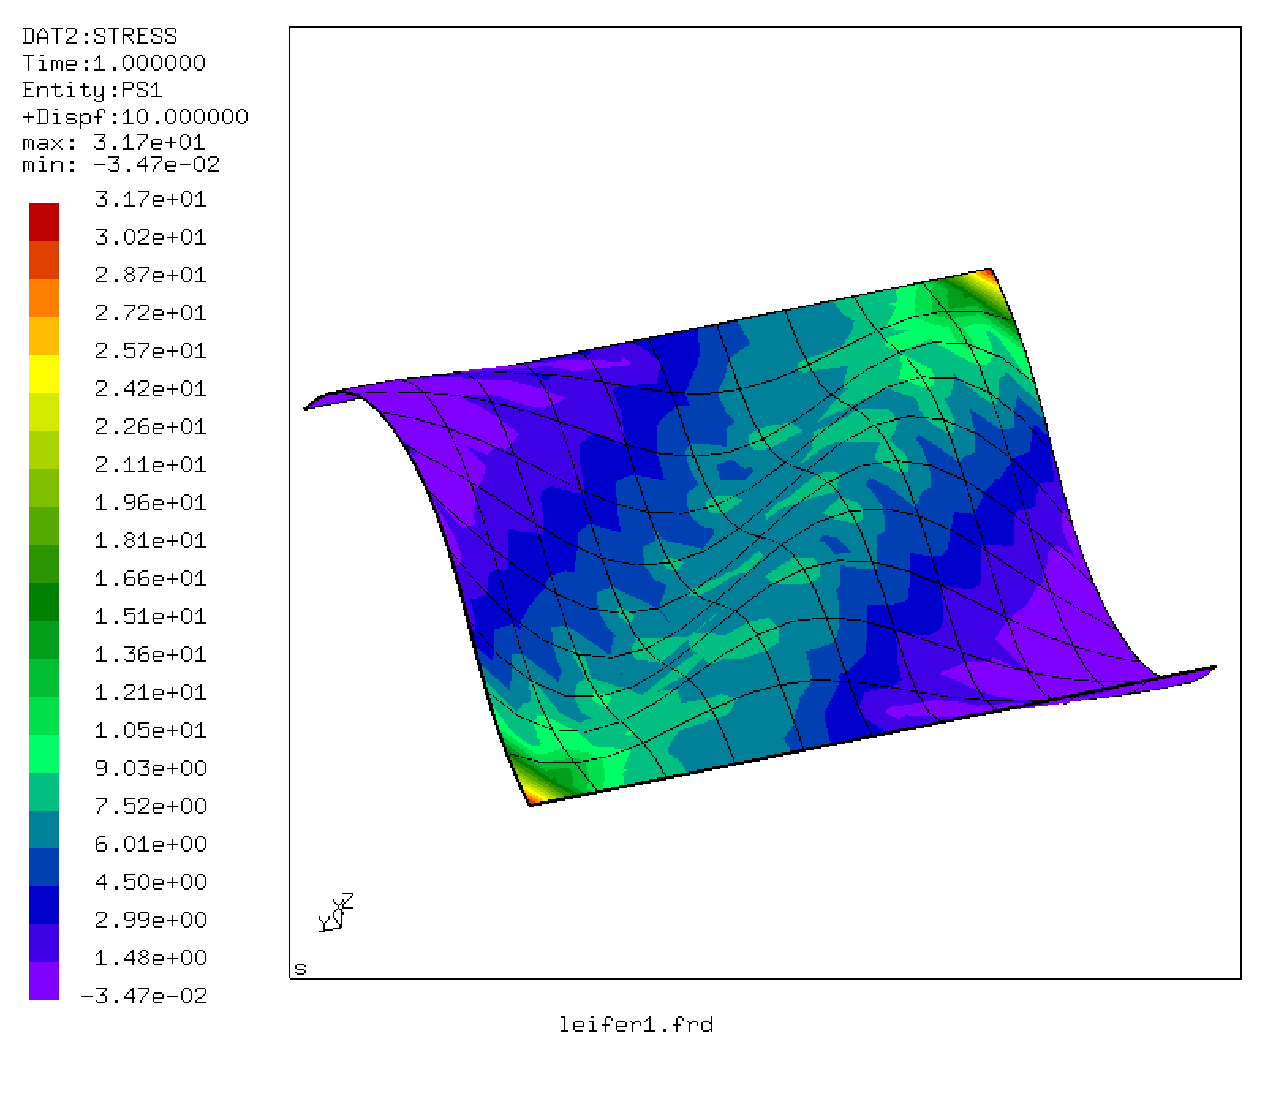
\epsfig{file=leifer1.eps,width=10cm}
\caption{\label{leifer1}Maximum principal stress in the deformed sheet}
\end{figure}

The input decks for this problem can be found in the test suite as leifer1.inp
and leifer2.inp. It was first devised by J. Leifer in 2003. The structure is a
thin square sheet with an edge length of 229 mm and a thickness of 0.0762
mm. It is fixed on one side and moved parallel to this side on the opposite
side by 1 mm. Young's modulus and Poisson's coefficient are 3790 MPa and 0.38,
respectively. Experimental evidence points to the creation of wrinkles due to
this shear deformation.

Here, two approaches are described to simulate this experiment. In both cases
the sheet is simulated using quadratic shell elements. In the first simulation
(leifer1) the material is considered as a linear elastic isotropic material, and
wrinkling occurs due to natural buckling processes in the
sheet. To enhance this buckling, the coordinates in the direction
perpendicular to the sheet (this is the z-direction in our simulation) are
slightly perturbed in a aleatoric way (look at the coordinates in the input
deck to verify this). Furthermore, the simulation is performed in a dynamic
procedure starting with very small time steps. Figure \ref{leifer1} shows the
maximum principal stress in the deformed sheet (the edge at x=0 was
fixed, the edge at x=229 was moved 1 mm in negative y-direction). One nicely notices the
wrinkles. A look at the smallest principal stress shows that there are
virtually no pressure stresses in the sheet: they were removed by buckling. A
disadvantage of this kind of simulation is the very long computational time
(336 increments for a step time of 1!). 

\begin{figure}
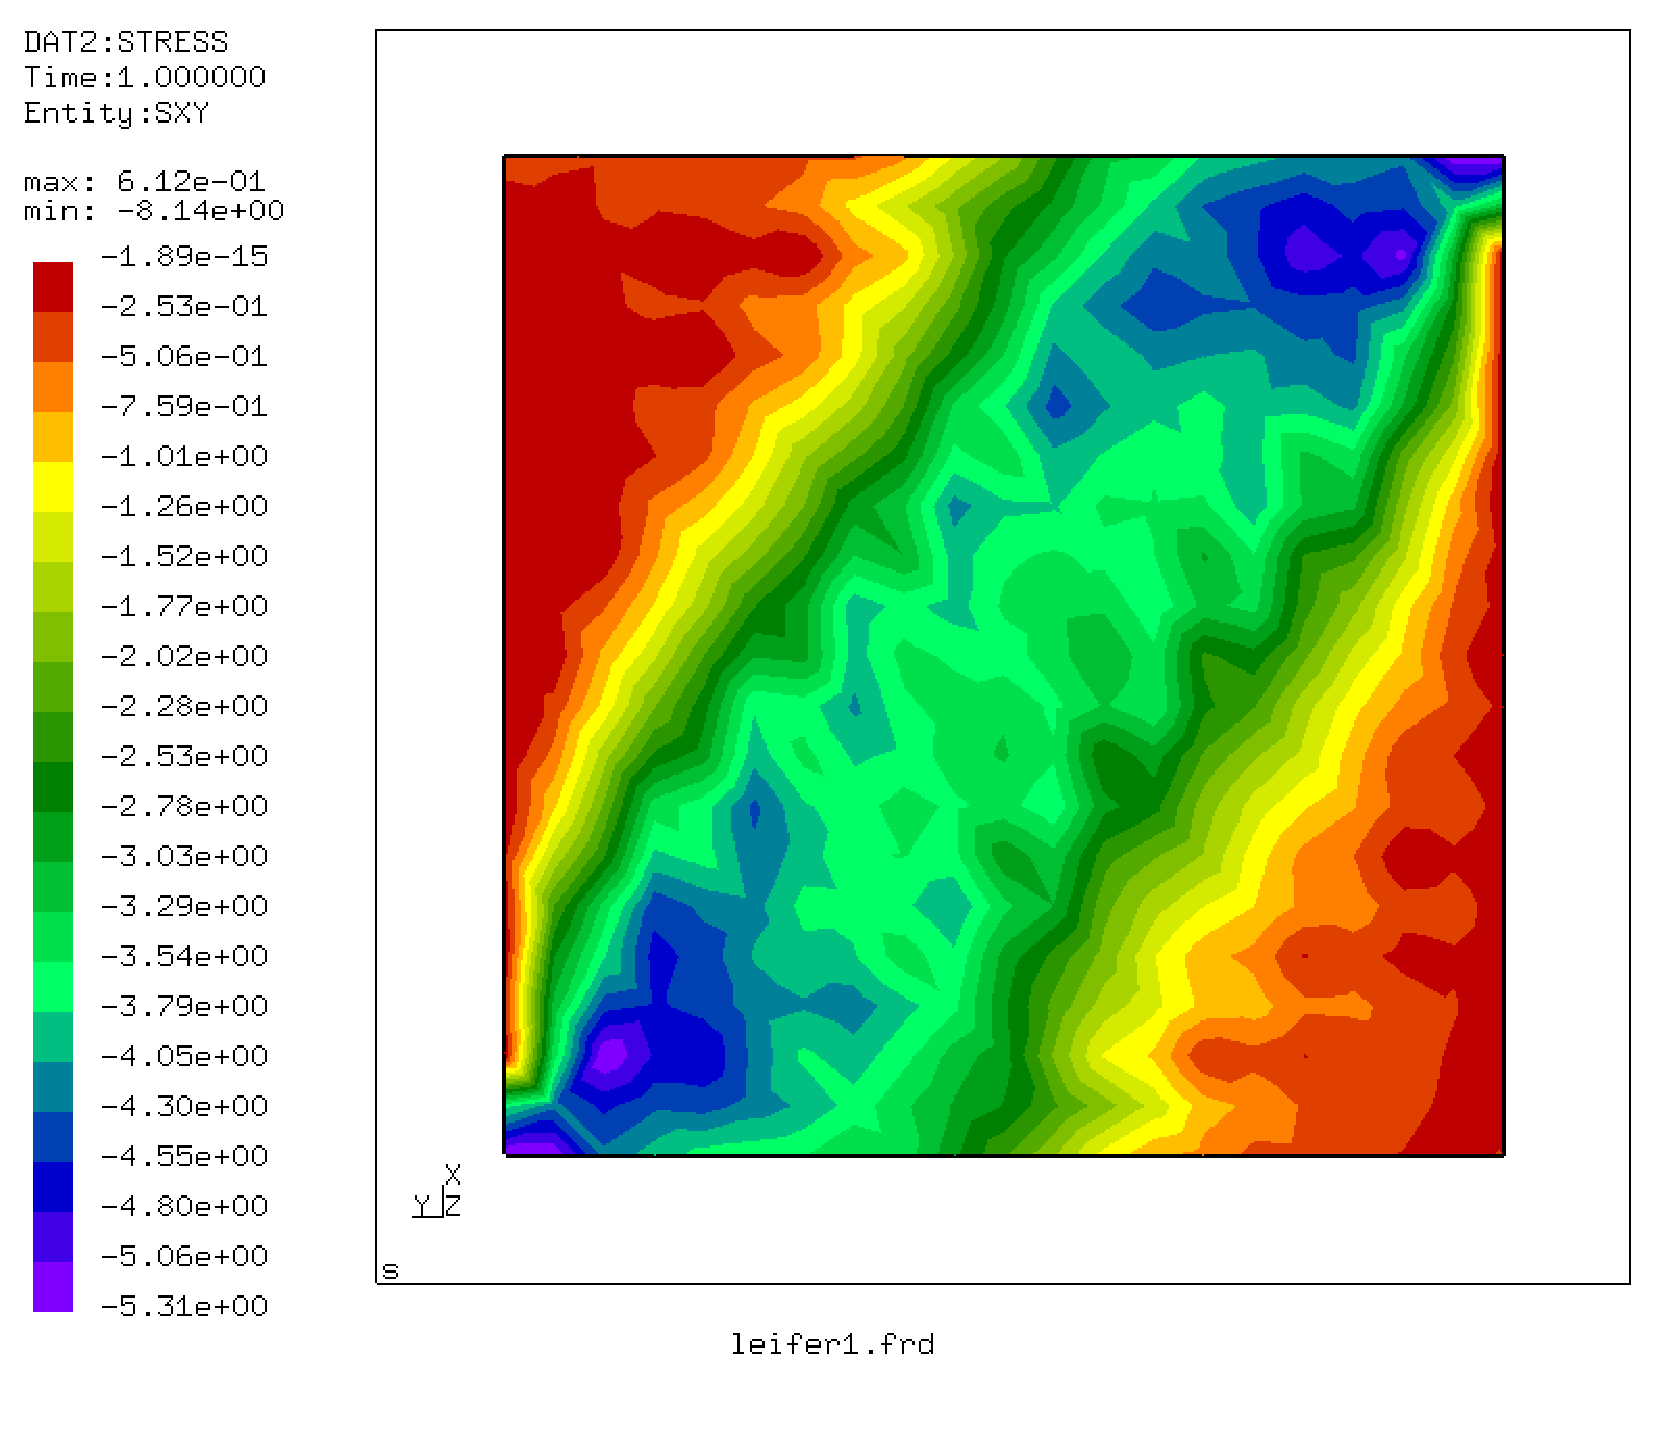
\epsfig{file=leifer2.eps,width=6cm}
\caption{\label{leifer2}Shear stress in the isotropic simulation}
\end{figure}

\begin{figure}
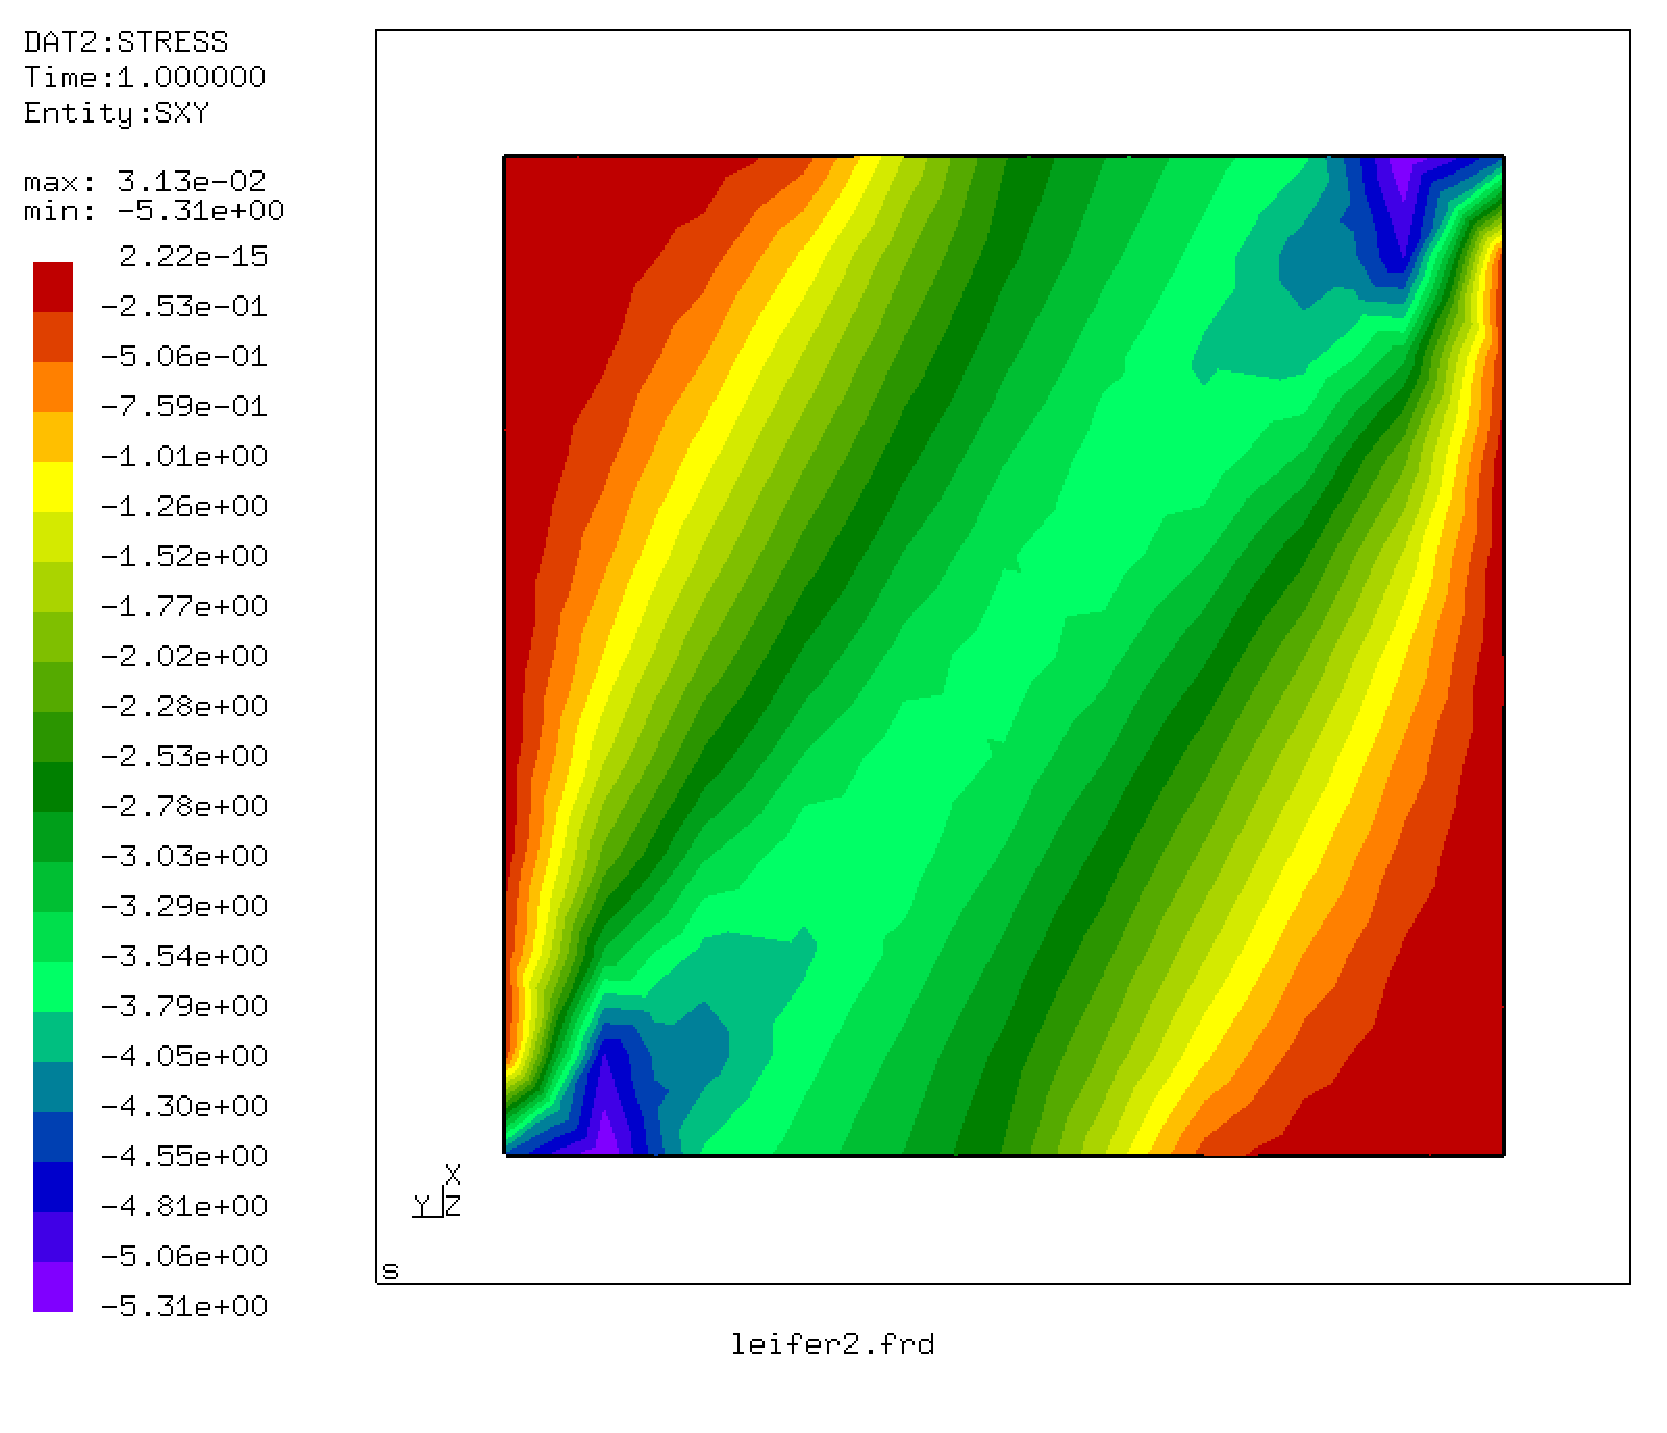
\epsfig{file=leifer3.eps,width=6cm}
\caption{\label{leifer3}Shear stress in the tension-only simulation}
\end{figure}

\begin{figure}
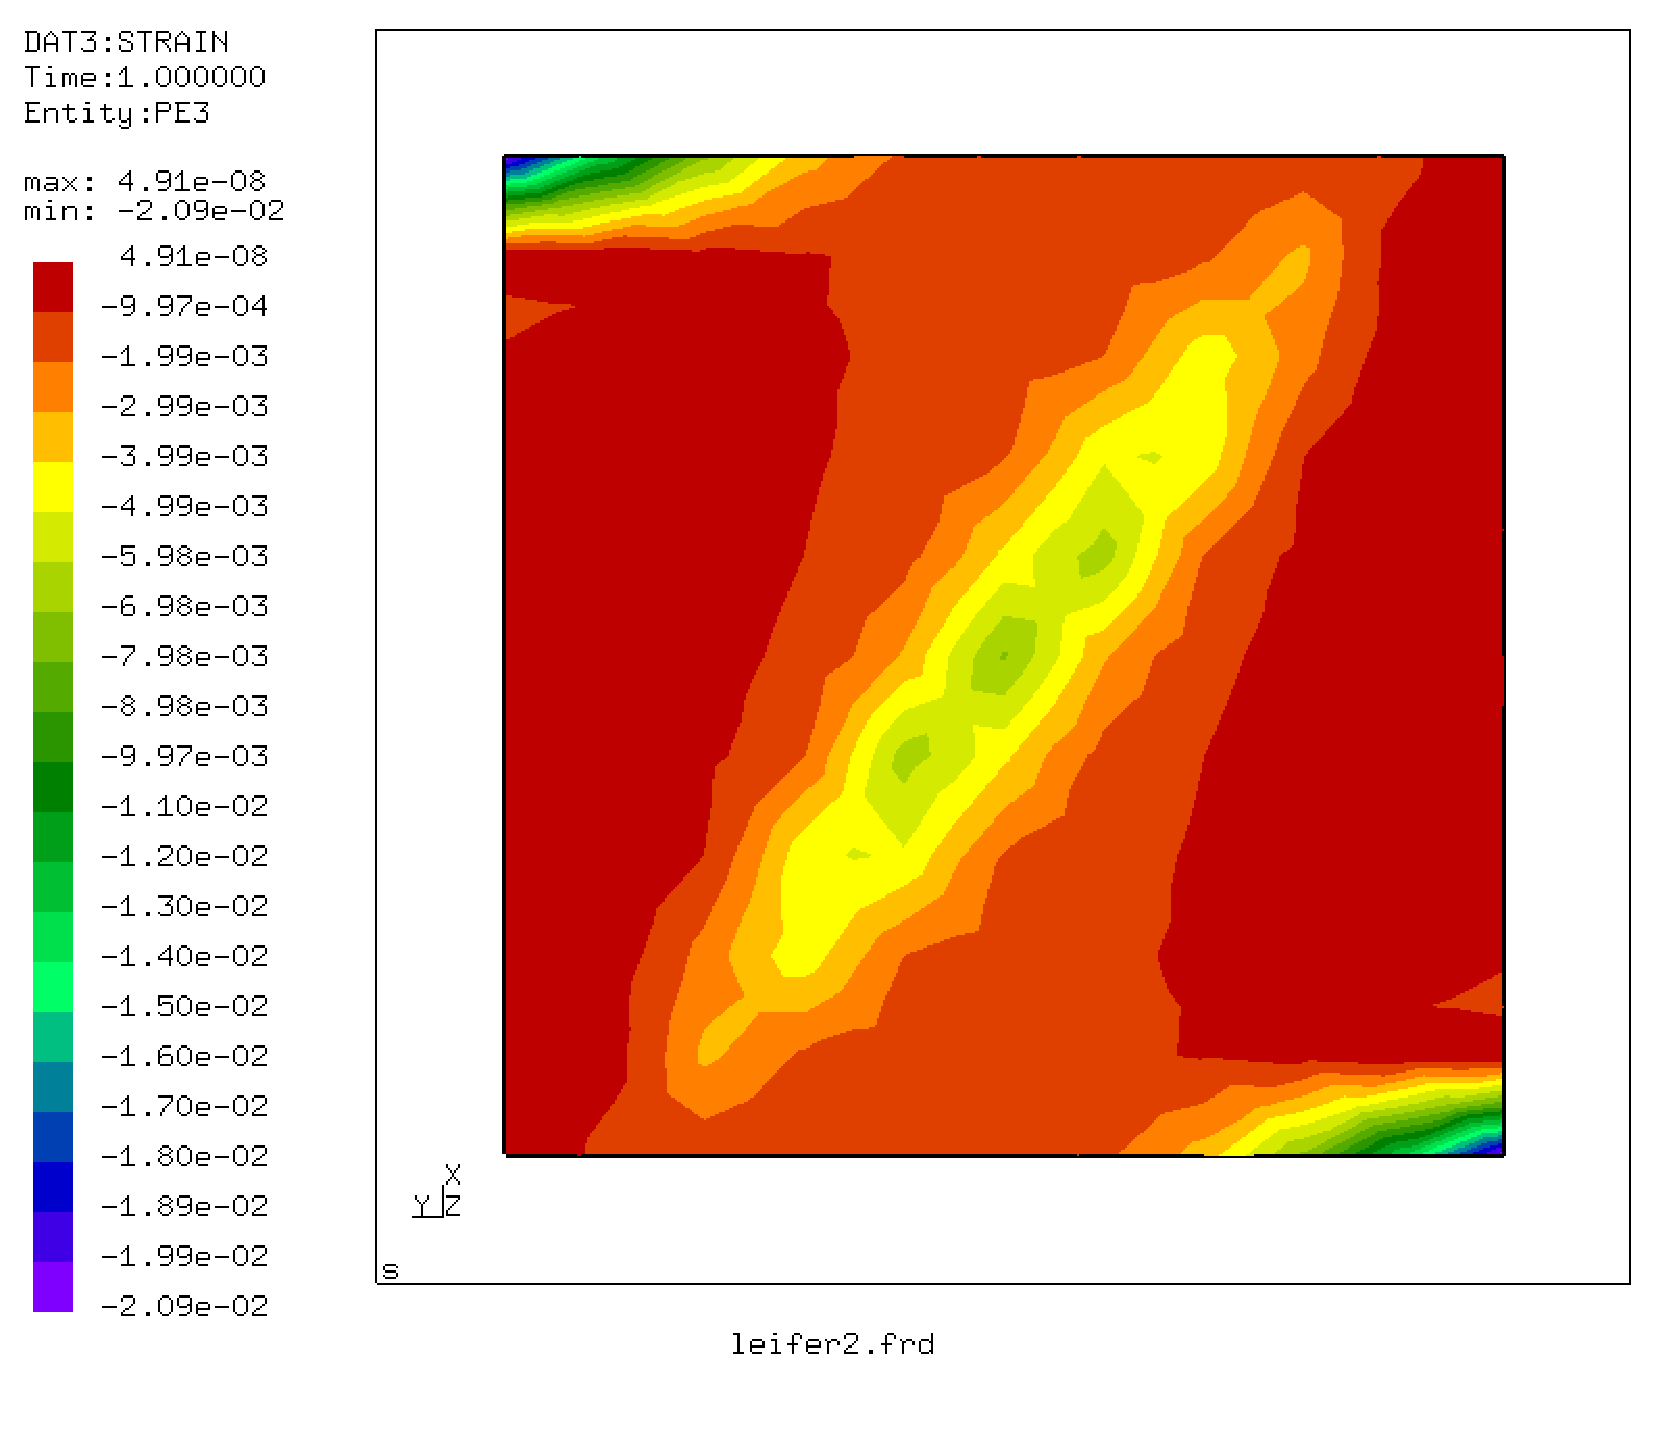
\epsfig{file=leifer5.eps,width=6cm}
\caption{\label{leifer5}Minimum principal strain in the tension-only simulation}
\end{figure}

The absence of pressure stress points to a second way of obtaining the correct
stress distribution: instead of simulating the material as isotropic, one can
use a tension-only material model (leifer2). This has the advantage that convergence is
much faster (small computational times). Figures \ref{leifer2} and \ref{leifer3} compare the shear
stress of both simulations: they match quite nicely (the shear stress
distribution in an isotropic simulation without wrinkling is totally
different). The same applies to the other stress components. The use of a
tension-only material, however, does not lead to out-of-plane
deformations. Here, wrinkling can only be derived indirectly by looking at the
smallest principal strain (Figure \ref{leifer5}). The large negative values
point to the existence of wrinkles.  

\subsection{Optimization of a simply supported beam}

In this section the optimization of a simply supported beam w.r.t. stress
and subject to a non-increasing mass constraint is treated. This example
shows how an optimization might be performed, the procedure itself is manually
and by no way optimized. For industrial applications one would typically write
generally applicable scripts taking care of the manual steps explained here.

This example uses the files opt1.inp, opt1.sh, opt2.fbl and op3.inp,
all available in the CalculiX test suite. File opt1.inp contains the geometry
and the loading of the problem at stake: the structure is a beam simply
supported at its ends (hinge on one side, rolls on the other) and a point
force in the middle. The von Mises stresses are shown in Figure \ref{opt1}.

\begin{figure}
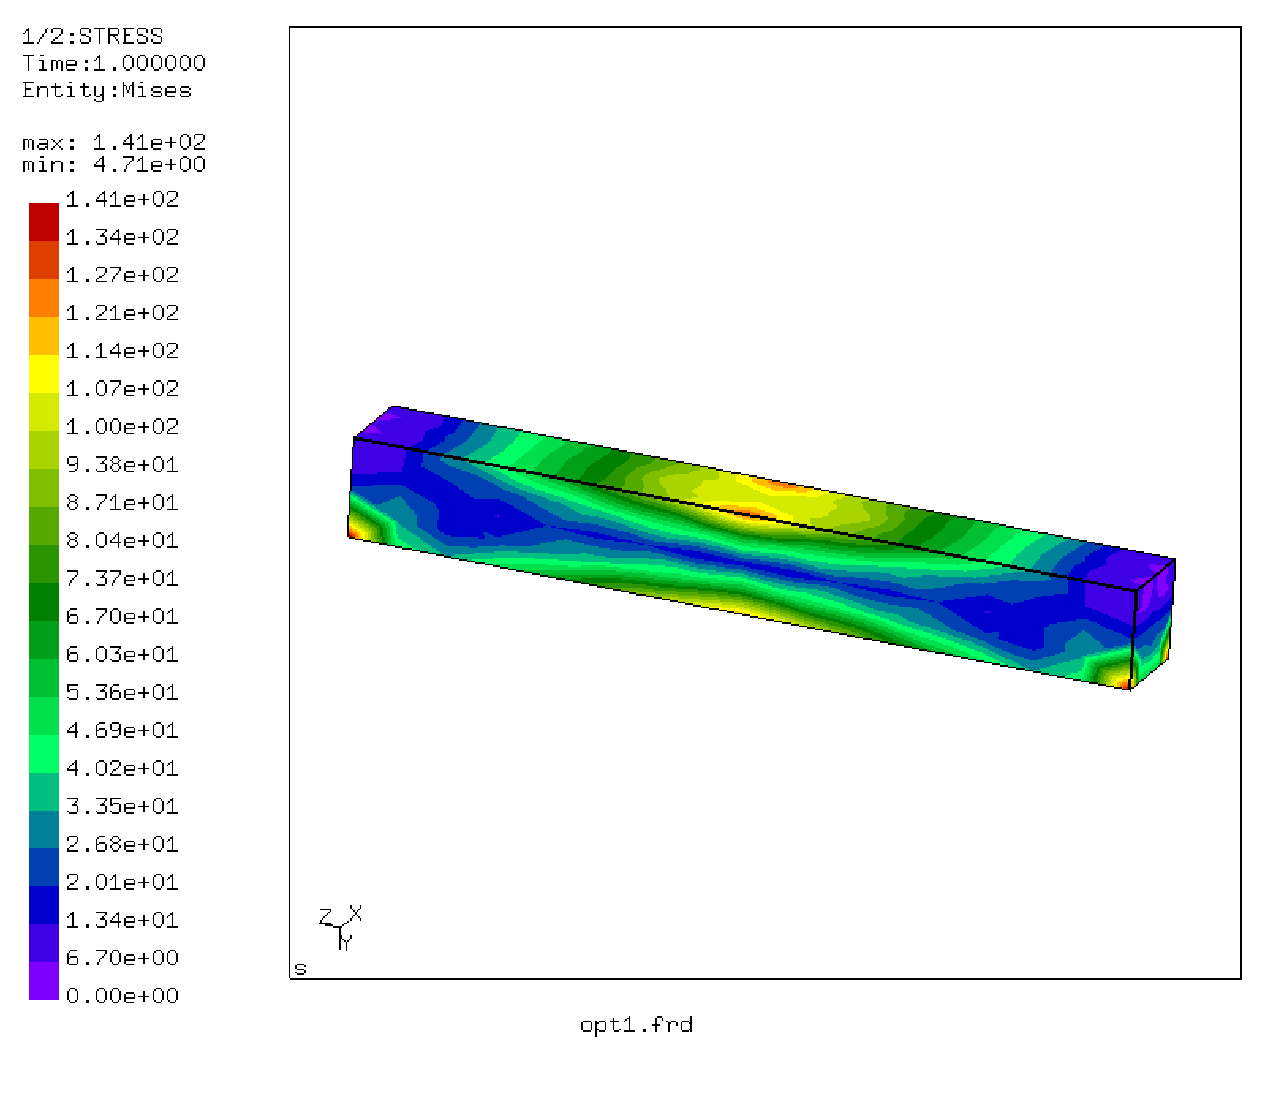
\epsfig{file=opt1.eps,width=10cm}
\caption{\label{opt1}von Mises stress in the starting geometry of the beam}
\end{figure}

The target of the optimization is to reduce the stresses in the beam. The
highest stresses occur in the middle of the beam and at the supports
(cf. Figure \ref{opt1}). Since the stresses at the supports will not decrease
due to a geometrical change of the beam (the peak stresses at the supports are
cause by the point-like nature of the support) the set of design variables
(i.e. the nodes in which the geometry of the beam is allowed to change during
the optimization) is chosen as all nodes in the beam except for a set of nodes in the vicinity
of the supports. These latter nodes are shown in Figure \ref{opt2}.

\begin{figure}
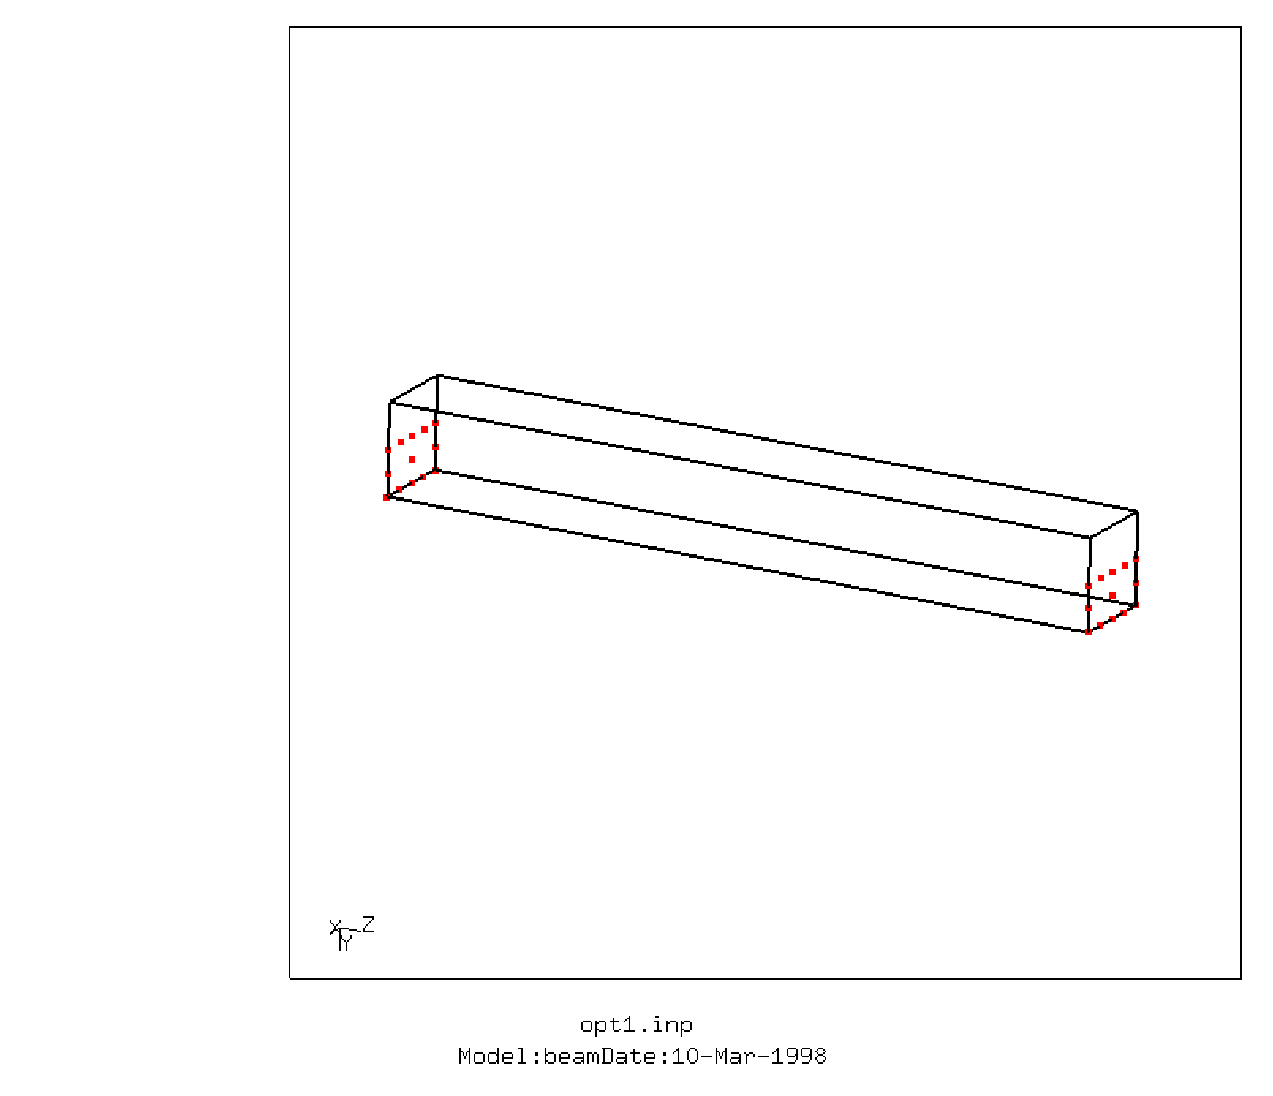
\epsfig{file=opt2.eps,width=6cm}
\caption{\label{opt2}Nodes excluded from the set of design variables}
\end{figure}

In order to perform an optimization one has to determine the sensitivity of
the objective w.r.t. the design variables taking into account any constraints
for every intermediate design step (iteration) of the optimization. The
objective and the constraints are generally design responses. First, the
sensitity of each design response is determined in a
\htmlref{*SENSITIVITY}{sensitivity} step. Then, one design response is
selected as objective and one or more as constraints in a \htmlref{*FEASIBLE
  DIRECTION}{feasibledirection} step. In the latter step the sensitivity of the
unconstrained objective is combined with the sensitity of the constraints in order to obtain
the sensitivity of the constrained objective.

The design variables were already discussed and constitute the set of nodes in
which the design is allowed to change. In the input deck for the present
example this is taken care of by the lines:

\begin{verbatim}
*DESIGNVARIABLES,TYPE=COORDINATE
DESIGNNODES
\end{verbatim}

``DESIGNNODES'' is a nodal set containing the design nodes as previously
discussed. For optimization problems in which the geometry of the structure is
to be optimized the type is COORDINATE. Alternatively, one could optimize the
orientation of anisotropic materials in a structure, this is covered by
TYPE=ORIENTATION. 

The objective is the design response one would like to minimize. In the present
example the Kreisselmeier-Steinhauser function calculated from the von Mises
stress in all design nodes (cf. \htmlref{*DESIGN RESPONSE}{designresponse} for the
definition of this function) is to be minimized. Again, the support nodes are
not taken into account because of the local stress singularity. The objective
is taken care of by the lines:

\begin{verbatim}
*DESIGN RESPONSE, NAME=STRESS_RESP
MISESSTRESS,DESIGNNODES,10.,100.
\end{verbatim}

in the sensitivity step and 

\begin{verbatim}
*OBJECTIVE,TARGET=MIN
STRESS_RESP
\end{verbatim}


in the feasible direction step in the input deck. Notice that the node set used to define the
Kreisselmeier-Steinhauser function (second entry underneath the *DESIGN
RESPONSE card) does not have to coincide with the set of
design variables. The third and
fourth entry underneath the *DESIGN RESPONSE card constitute parameters in the
Kreisselmeier-Steinhauser function. Specifically, the fourth entry is a
reference stress value and should be of the order of magnitude of the actual
maximum stress in the model. The third parameter allows to smear the maximum
stress value in a less or more wide region of the model. 

In addition to the objective function (only one objective function is allowed)
one or more constraints can be defined in the feasible direction step. In the actual example the mass of the
beam should not increase during the optimization. This is taken care of by

\begin{verbatim}
*DESIGN RESPONSE, NAME=MASS_RESP
MASS,Eall
\end{verbatim}

in the sensitivity step and

\begin{verbatim}
*CONSTRAINT
MASS_RESP,LE,1.,
\end{verbatim}

in the feasible direction step. For the meaning of the entries the reader is referred to
\htmlref{*DESIGN RESPONSE}{designresponse} and \htmlref{*CONSTRAINT}{constraint}. Notice that for this constraint to be active
the user should have defined a density for the material at stake. Within
CalculiX the constraint is linearized. This means that, depending on the
increment size during an optimization, the constraint will not be satisfied exactly.

In the CalculiX run the sensitivity of the objective and all
constraints w.r.t. the design variables is calculated. The sensitivity is
nothing else but the first derivative of the objective function w.r.t. the
design variables (similarly for the constraints), i.e. the sensitivity shows
how the design response changes if the design variable is changed. For
design variables of type COORDINATE the change of the design variables
(i.e. the design nodes) is in a direction locally orthogonal to the
geometry. So in our case the sensitivity of the stress tells us how the stress
changes if the geometry is changed in direction of the local normal (similar
with the mass CONSTRAINT). If the
sensitivity is positive the stress increases while thickening the structure and
vice versa. This sensitivity may be postprocessed by using a filter. In the
present input deck (opt1.inp) the following filter is applied:

\begin{verbatim}
*FILTER,TYPE=EXPLICIT,EDGE PRESERVATION=YES,DIRECTION WEIGHTING=YES
3.
\end{verbatim}

\begin{figure}
  \centering
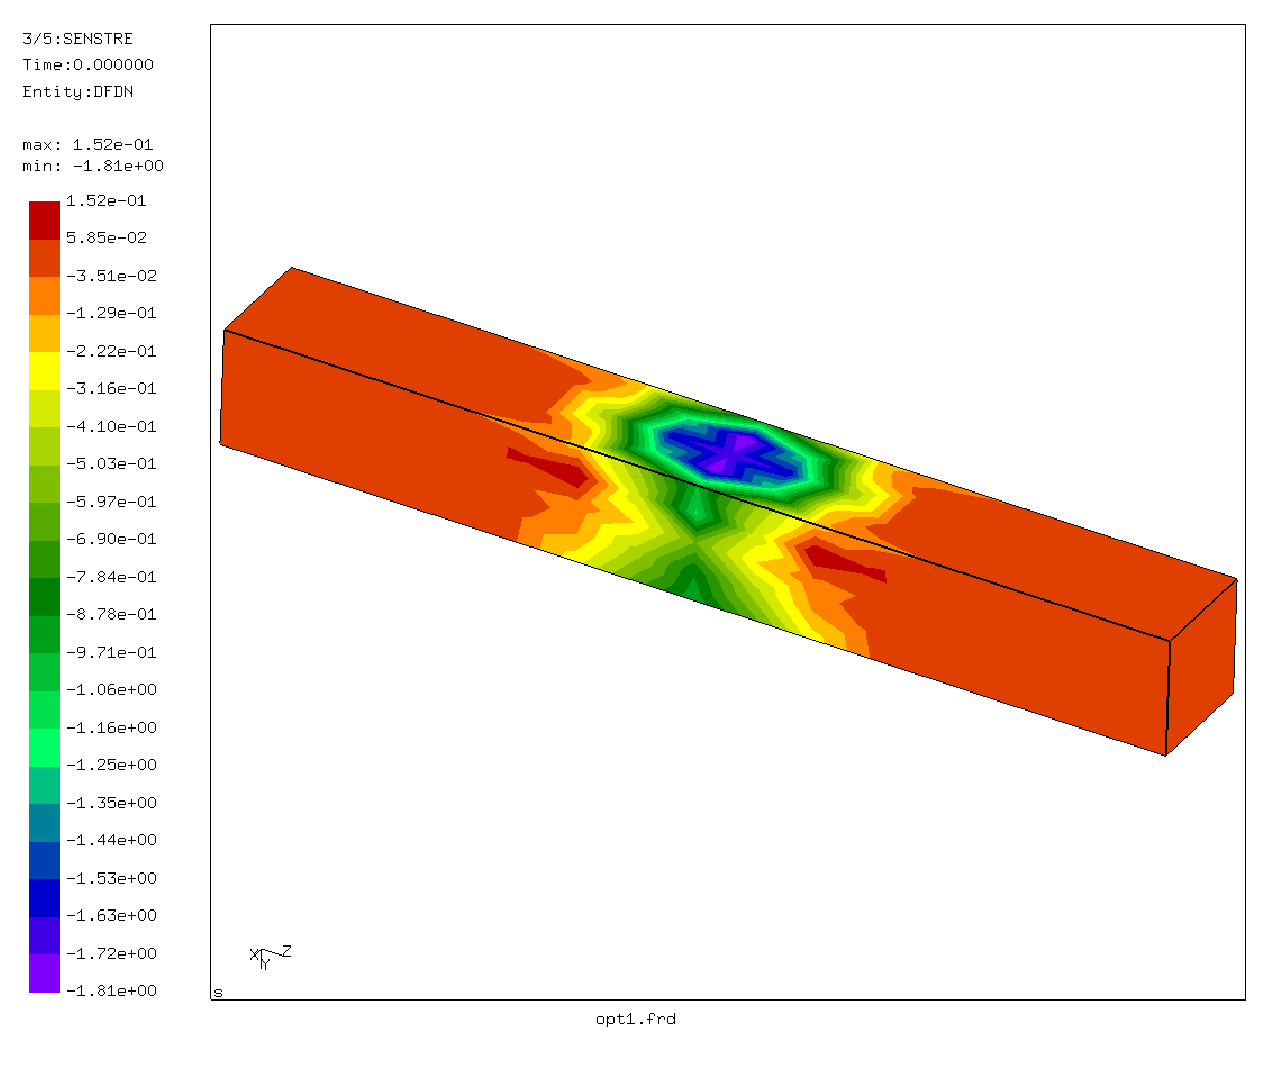
\epsfig{file=opt3.eps,width=6cm}
\caption{\label{opt3}Stress sensitivity before filtering}
\end{figure}

\begin{figure}
  \centering
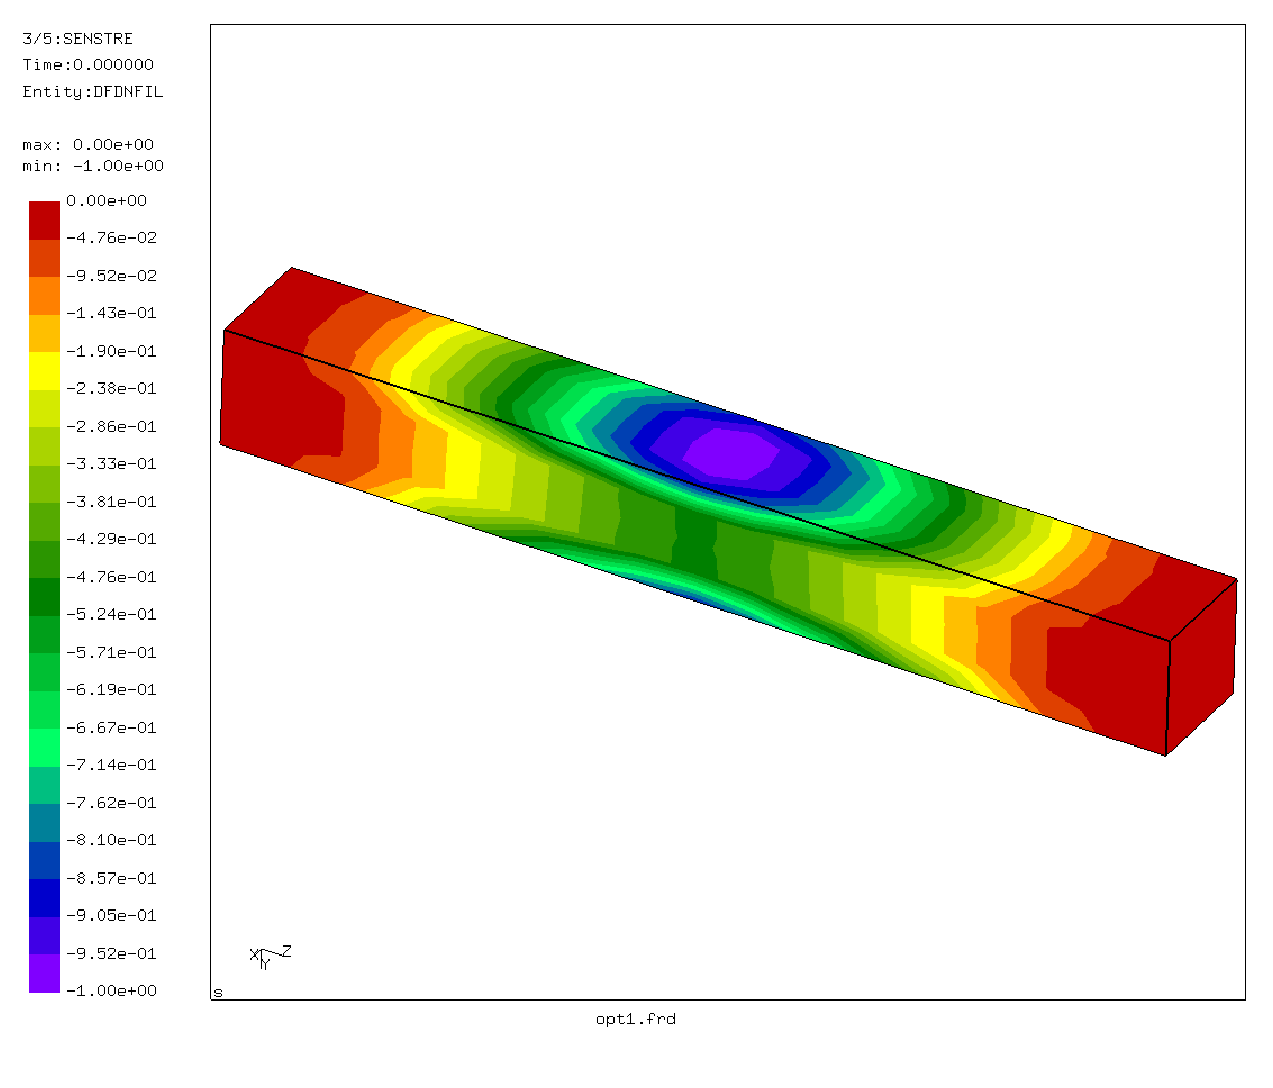
\epsfig{file=opt4.eps,width=6cm}
\caption{\label{opt4}Stress sensitivity after filtering}
\end{figure}

\begin{figure}
  \centering
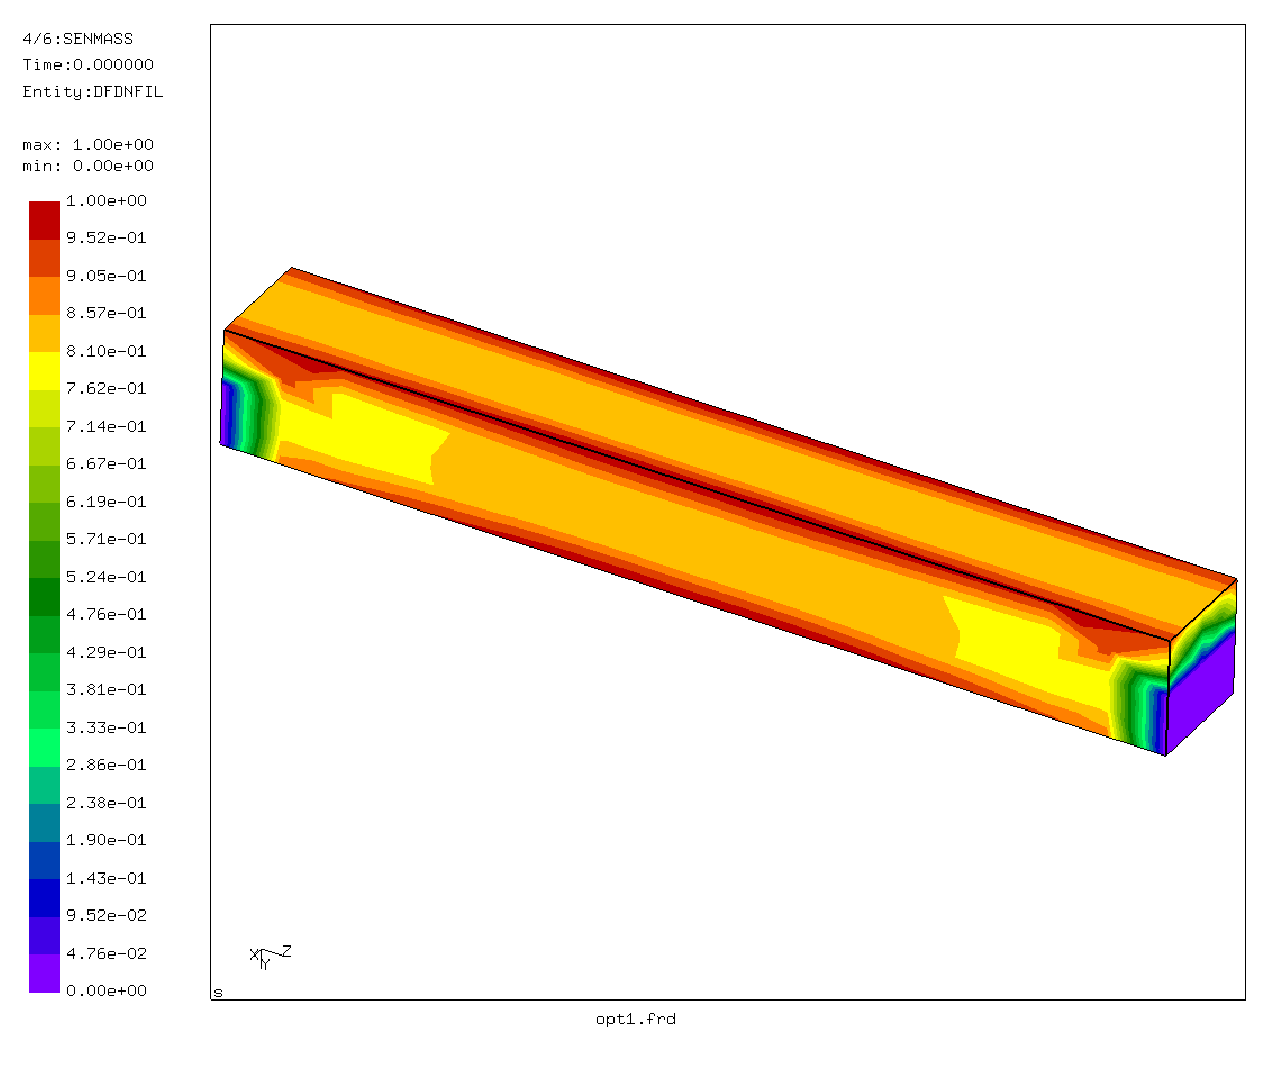
\epsfig{file=opt5.eps,width=6cm}
\caption{\label{opt5}Mass sensitivity after filtering}
\end{figure}
 
The filter chosen to be explicit. For the filter, which is by default linear,
a radius of 3 has been selected (it can be visualized as a cone at each design variable
in which the sensitivity is integrated and subsequently smeared), sharp
corners should be kept (EDGE PRESERVATION=YES, cf. \htmlref{*FILTER}{filter})
and surfaces with a clearly different orientation (e.g. orthogonal) are not
taken into account while filtering (or taken into account to a lesser degree,
DIRECTION WEIGHTING=YES). The filtering is applied to each design response separately. Figure \ref{opt3} shows the stress
sensitivity before filtering, Figure \ref{opt4} the stress sensitivity after
filtering and Figure \ref{opt5} the mass sensitivity after filtering. All of
this information is obtained by requesting SEN underneath the *NODE FILE
card. 

\begin{figure}
  \centering
\epsfig{file=opt6.eps,width=6cm}
\caption{\label{opt6}Stress sensitivity taking the mass constraint into account}
\end{figure}

After calculating the filtered sensitivities of the objective function and the
constraints separately (this is done in the sensitivity step) they are joined by projecting the sensitivity of the active constraints
on the sensitivity of the objective function (this is done in the feasible
direction step). For a mesh modification size of 1 (parameter underneath the
*FEASIBLE DIRECTION card) this results in Figure
\ref{opt6}.

The sensitivities calculated in this way allow us to perform an
optimization. The simplest concept is the steepest gradient algorithm in which
the geometry is changed in the direction of the steepest gradient. In
the present calculations only one gradient is calculated (the one in the
direction of the local normal) since a geometry change parallel to the surface
of the structure generally does not change the geometry at all. So the
geometry is changed in the direction of the local normal by an amount to be
defined by the user. It is usually a percentage of the local sensitivity, the
so-called mesh modification size, to be defined underneath the *FEASIBLE
DIRECTION card. Here, a mesh modification size of 10 \% was selected
(i.e. 0.1). 

In order to maintain a good quality mesh the other boundary
nodes and the internal nodes should be appropriately moved as well. This is
taken care of by a subsequent linear elastic calculation with the
sensitivity-based surface geometry change as boundary conditions. The
corresponding input deck with the name opt1.equ is automatically generated
within the *FEASIBLE DIRECTION step.

This input deck contains the original geometry of the beam. The
sensitivity-based surface geometry change is imposed by *BOUNDARY statements.

Furthermore, preservation of sharp edges and corners in the original structure
is taken care of by linear equations. In order to obtain a good quality mesh
at the free surface the fictitious elastic modulus is decreased with
increasing distance from the free surface. Before running opt1.equ it is
copied by script opt1.sh into opt2.inp.

\begin{figure}
  \centering
\epsfig{file=opt7.eps,width=6cm}
\caption{\label{opt7}Deformed mesh after one iteration}
\end{figure}

\begin{figure}
  \centering
\epsfig{file=opt8.eps,width=10cm}
\caption{\label{opt8}Mises stress after one iteration}
\end{figure}

The resulting deformed mesh is shown in Figure \ref{opt7}. The beam was
thickened in the middle, where the von Mises stresses were highest. This
should lead to a decrease of the highest stress value. In order to check this,
a new sensitivity calculation was done on the deformed structure. To that end
the deformation calculated based on opt2.inp is superimposed on the
coordinates (by a call to opt2.fbl in script opt1.sh) and stored as opt3.inc. This file is included in input deck
opt3.inp, which apart from the coordinates is a copy of opt1.inp. The resulting von Mises stresses are shown in Figure
\ref{opt8}. The von Mises stress in the middle of the lower surface of the
beam has indeed decreased from 114 to about 83 (MPa if the selected units were
mm, N, s and K). Further improvements can be obtained by running several iterations.

\subsection{Mesh refinement of a curved cantilever beam}

This example illustrates the use of the *REFINE MESH keyword card in order to
refine a tetrahedral mesh based on some solution variable. The structure is a
curved cantilever beam (Figure \ref{refine1}) meshed very coarsely using C3D10
elements. The left side of the beam is completely fixed in z-direction, the
lower left node is furthermore fixed in x and y, the lower right node in
y. A load of 9 force units is applied to the nodes in the right face of the
beam in +y direction. This leads to the normal stresses in z shown in the
Figure. The beam experiences bending leading to tensile stresses at the bottom
and compressive stresses at the top. The input deck of the beam (circ10p.inp)
is part of the CalculiX test suite.

\begin{figure}
\epsfig{file=refine1.eps,width=10cm}
\caption{\label{refine1}Normal stress in z-direction for the coarse mesh}
\end{figure}

\begin{figure}
\epsfig{file=refine2.eps,width=10cm}
\caption{\label{refine2}Error estimator for the coarse mesh}
\end{figure}

Here, only the step information in the input deck is reproduced:

\begin{verbatim}
*STEP
*STATIC
*CLOAD
LOAD,2,1.
*NODE PRINT,NSET=FIX,TOTALS=ONLY
RF
*SECTION PRINT,SURFACE=Sfix,NAME=SP1
SOF,SOM
*NODE FILE
U
*EL FILE
S
*REFINE MESH,LIMIT=50.
S
*END STEP
\end{verbatim}

It illustrates several possibilities to obtain the reaction forces. One way is
to use the *NODE PRINT keyword card to request the storage of RF in the .dat
file. It acts on a node set, in this case all nodes on the left surface of the
beam. The parameter TOTALS=ONLY indicates that only the sum of the forces
should be printed, not the individual contributions. The *NODE PRINT option
works well if the adjacent elements of the nodal set are not subject to
distributed loads, neither surface distributed loads (pressure) nor volumetric
distribute loads (gravity, centrifugal forces). Else the value printed for RF
will include part of these latter forces. 

A second possibility is to define a facial surface and use SOF and SOM
underneath the *SECTION PRINT card in order to request the forces and moments
on this surface. The surface Sfix consists of all faces in the left surface of
the beam. The forces and moments are obtained by integration across the
surface.

The output in the .dat-file looks like:
\begin{verbatim}

 total force (fx,fy,fz) for set FIX and time  0.1000000E+01

       -9.372063E-13 -9.000000E+00  3.127276E-12



 statistics for surface set SFIX and time  0.1000000E+01

   total surface force (fx,fy,fz) and moment about the origin(mx,my,mz)

    2.454956E+00 -7.226251E+00  1.377949E+01  7.236961E+01 -5.740438E+00 -4.957194E+00

   center of gravity and mean normal

    5.000000E-01  5.000000E-01  0.000000E+00  0.000000E+00  0.000000E+00 -1.000000E+00

   moment about the center of gravity(mx,my,mz)

    6.547987E+01  1.149306E+00 -1.165902E-01

   area,  normal force (+ = tension) and shear force (size)

    6.000000E+00 -1.377949E+01  7.631875E+00
\end{verbatim}

From this one observes that the reaction force obtained by the *NODE PRINT
statement is very accurate, however, the integration across the surface of the
stresses is rather inaccurate: instead of 9 force units one obtains 7.23
units. The moment about the center of gravity is 65.5 [force][length] instead
of the expected 72 [force][length] (the length of the beam is 8 length units).

The value of the error estimator is shown in Figure \ref{refine2}. Not
surprisingly, the error is quite high, up to 30 \%. 

In order to obtain better results, an automatic stress-based refinement is
triggered by the *REFINE MESH,LIMIT=50 card. The field on which the refinement
is based is listed underneath this card. ``S'' means that the Mises stress
will be used. The Mises stress for this example reaches values of about 400
stress units, so a refinement of up to a factor of 8 is locally possible (a
refinement limit of 50. was chosen). In the current version of CalculiX up to
three iterations are performed, each of which allows for a refinement by a
factor of two. The refinements are always applied to a version of the original
mesh in which any quadratic elements are replaced by linear ones (C3D10 by
C3D4), i.e. the middle nodes are not taken into account. The results of these
refinement iterations are stored as input decks (containing only the mesh) in
files finemesh.inp0, finemesh.inp1 and finemesh.inp2. After generating the
mesh stored in finemesh.inp2, the program generates midnodes for all elements
if the input deck contained at least one quadratic element. All nodes are
subsequently projected onto the faces of the original mesh. This means that
the geometry is basically described by the outer surface of the mesh in the
input deck. Elements in the input deck other than tetrahedral elements remain
untouched. The resulting projected mesh is stored as input deck in
jobname.fin. It contains only the refined mesh (nodes and elements).

Running the circ10p input deck and reapplying the necessary boundary and
loading conditions (this has to be done by hand) leads to the input deck
cric10pfin.inp (also part of the CalculiX test examples). Running this deck
leads to the normal z-stresses in Figure \ref{refine3} and the error in Figure \ref{refine4}.

\begin{figure}
\epsfig{file=refine3.eps,width=10cm}
\caption{\label{refine3}Normal stress in z-direction for the fine mesh}
\end{figure}

\begin{figure}
\epsfig{file=refine4.eps,width=10cm}
\caption{\label{refine4}Error estimator for the fine mesh}
\end{figure}

The mesh has been refined near the left face of the beam, where the stresses
were highest. The resulting elements are quadatic elements and the curvature
of the original mesh has been nicely kept. 

The compressive stresses are slightly increased, while the tensile stresses
are now much more localized about the nodes fixed in y-direction. The overall
level, however, is similar. The stress error is about the same as for the
coarse mesh, however, at those locations where the stress is high, the error
is now low, about 5 \% instead of 30 \%. These are the locations of interest.

The output for the reaction forces in the .dat file looks like: 
\begin{verbatim}

 total force (fx,fy,fz) for set FIX and time  0.1000000E+01

        3.221013E-12 -9.000000E+00  7.356782E-12



 statistics for surface set SFIX and time  0.1000000E+01

   total surface force (fx,fy,fz) and moment about the origin(mx,my,mz)

    1.512388E-01 -9.252627E+00 -7.227514E-01  7.175724E+01  1.563390E-01 -4.206416E+00

   center of gravity and mean normal

    5.000000E-01  5.000000E-01  4.014218E-19 -4.263022E-20  4.286885E-20 -1.000000E+00

   moment about the center of gravity(mx,my,mz)

    7.211862E+01 -2.050367E-01  4.955169E-01

   area,  normal force (+ = tension) and shear force (size)

    6.000000E+00  7.227514E-01  9.253863E+00
\end{verbatim}

The nodal output is again very accurate, while the section output has clearly
improved: the total reaction force is now -9.25 force units, the moment about
the center of gravity is 72.12 [force][length]. The finer mesh leads to more
accurate nodal stresses, which are the ones which have been used to determine
the section forces.

\section{Theory \label{strains}}
The finite element method is basically concerned with the determination of
field variables. The most important ones are the stress and strain fields. As
basic measure of strain in CalculiX the Lagrangian strain tensor E is used for
elastic media, the deviatoric elastic left Cauchy-Green tensor for incremental
plasticity, the logarithmic (or Hencky) strain \cite{Belytschko} for some
other plasticity models as deformation plasticity and Johnson-Cook hardening
and linear strains where appropriate, i.e. for small deformations combined
with small rotations. The Lagrangian strain satisfies (\cite{Eringen}):

\begin{equation}
E_{KL}=(U_{K,L}+U_{L,K}+U_{M,K} U_{M,L})/2,\;\;\;K,L,M=1,2,3
\end{equation}
where $U_K$ are the displacement components in the material frame of reference and repeated indices imply summation over the appropriate range. In a linear analysis, this reduces to the familiar form:

\begin{equation}
\tilde{E}_{KL}=(U_{K,L}+U_{L,K})/2,\;\;\;K,L=1,2,3.
\end{equation}

The deviatoric elastic left Cauchy-Green tensor is defined by (\cite{Simo1}):
\begin{equation}
\bar{b}^e_{kl}=J^{e-2/3}x^e_{k,K}x^e_{l,K}
\end{equation}

where $J^e$ is the elastic Jacobian and $x^e_{k,K}$ is the elastic deformation
gradient. Finally, the logarithmic strain satisfies:

\begin{equation}
  e_{\text{ln}}:= \sum_{i} \ln \lambda_i \boldsymbol{n}_i \otimes
  \boldsymbol{n}_i,
\end{equation}

where $\lambda_i^2$ are the eigenvalues of the Cauchy-Green tensor
$\boldsymbol{C}:= \boldsymbol{F}^T \cdot \boldsymbol{F}$ and $\boldsymbol{n}_i$ are
obtained from the eigenvectors $\boldsymbol{N}_i$ of $\boldsymbol{C}$ through

\begin{equation}
  \boldsymbol{n}_i = \boldsymbol{R}  \cdot \boldsymbol{N}_i,
\end{equation}

where $\boldsymbol{R}$ is the rotation tensor obtained from the well known
decomposition of the deformation gradient $\boldsymbol{F}$  into a product of an orthogonal
matrix $\boldsymbol{R}$ and a symmetric matrix $\boldsymbol{U}$ in the form 
$\boldsymbol{F}= \boldsymbol{R} \cdot \boldsymbol{U}$. The above formulas apply to Cartesian coordinate systems.

The stress measure consistent with the Lagrangian strain is the second
Piola-Kirchhoff stress $\boldsymbol{S}$. This stress, which is internally used in CalculiX
for all applications (the so-called total Lagrangian approach, see
\cite{Belytschko}), can be transformed into the first Piola-Kirchhoff stress
$\boldsymbol{P}$ 
(the so-called engineering stress, a non-symmetric tensor) and into the Cauchy
stress $\boldsymbol{\sigma } $ (true stress). All CalculiX input (e.g. distributed loading) and
output is in terms of true stress. The stress measures are related by:

\begin{equation}
  \boldsymbol{P} = J \boldsymbol{F}^{-1} \cdot \boldsymbol{\sigma }
\end{equation}

and

\begin{equation}
  \boldsymbol{S} = J \boldsymbol{F}^{-1} \cdot \boldsymbol{\sigma } \cdot
  \boldsymbol{F}^{-T}, 
\end{equation}

where $J=\det(\boldsymbol{F})$. 

The treatment of the thermal strain depends on whether the analysis is
geometrically linear or nonlinear. For isotropic material the thermal strain
tensor amounts to $\overline{\alpha} \Delta T \boldsymbol{I}$, where
$\overline{ \alpha}$ is the (secant)
expansion coefficient, $\Delta T$ is the temperature change since the initial
state and $\boldsymbol{I}$ is the second order identity tensor. For
geometrically linear calculations the thermal strain is subtracted from the
total strain to obtain the mechanical strain:

\begin{equation}
  \tilde{E}_{KL}^{\text{mech}} = \tilde{E}_{KL} - \overline{\alpha} \Delta T \delta_{KL}.
\end{equation}

In a nonlinear analysis the thermal strain is subtracted from the deformation
gradient in order to obtain the mechanical deformation gradient. Indeed,
assuming a multiplicative decomposition of the deformation gradient one can
write:

\begin{equation}
  d \boldsymbol{x} = \boldsymbol{F} \cdot d \boldsymbol{X} = \boldsymbol{F}_{\text{mech}} \cdot \boldsymbol{F}_{\text{th}} \cdot
  d \boldsymbol{X},
\end{equation}

where the total deformation gradient $\boldsymbol{F}$ is written as the
product of the mechanical deformation gradient and the thermal deformation
gradient. For isotropic materials the thermal deformation gradient can be
written as $\boldsymbol{F}_{\text{th}}=(1+\overline{\alpha} \Delta T) \boldsymbol{I}$ and
consequently:

\begin{equation}
  \boldsymbol{F}_{\text{th}}^{-1} \approx (1-\overline{\alpha} \Delta T) \boldsymbol{I}.
\end{equation}

\noindent Therefore one obtains:

\begin{eqnarray}
  (F_{\text{mech}})_{kK}  &\approx  & F_{kK}(1-\overline{\alpha} \Delta T) =
  (1+u_{k,K})(1-\overline{\alpha} \Delta T) \nonumber \\
   &\approx & 1+u_{k,K}-\overline{\alpha} \Delta T.
\end{eqnarray}

Based on the mechanical deformation gradient the mechanical Lagrange strain is
calculated and subsequently used in the material laws:

\begin{equation}
2 \boldsymbol{E}_{\text{mech}} = \boldsymbol{F}_{\text{mech}}^T \cdot
\boldsymbol{F}_{\text{mech}} - \boldsymbol{I}.
\end{equation}

Since the stretches $\lambda$ are the eigenvalues of the deformation
gradient, subtracting $\overline{\alpha} \Delta T \boldsymbol{I}$ from $\boldsymbol{F}$
amounts to subtracting $\overline{\alpha} \Delta T$ from $\lambda = L/L_0 = 1 + \Delta
L/L_0$. Therefore, the thermal strain get the meaning of a length change
divided by an initial length. Infinitesimally one obtains:

\begin{equation}
  \frac{dL}{L_0} = \alpha d T,
\end{equation}

leading to

\begin{eqnarray}
  \frac{L-L_0}{L_0} &=& \int_{T_0}^{T} \alpha (\xi) d \xi \nonumber \\
  &=:& \overline{\alpha }(T) (T-T_0)   \nonumber \\
  &=& \overline{\alpha } (T) \Delta T,
\end{eqnarray}

from which

\begin{equation}
  L = L_0 ( 1 + \overline{\alpha }(T) \Delta T.
\end{equation}

Here, $T_0$ is the temperature for which the specimen length is $L_0$,
$\alpha$ is the instantaneous or tangent expansion coefficient and
$\overline{\alpha }$ is the secant expansion coefficient. We
observe that the extension is linear in the temperature. This is also the way
in which the expansion coefficients are usually measured, i.e. with respect to
the initial specimen length.

Notice that the same approach is taken in CalculiX for the calculation of the
corotational logarithmic strain needed for an Abaqus User Material
Routine. First, the thermal strain is subtracted from the total stretch to
obtain the mechanical stretch and then the corational logarithmic mechanical strain is
built:

\begin{equation}
  \hat{E}_{\text{ln,mech}} = \sum_{i} \ln \lambda_{\text{mech},i}
  \boldsymbol{N}_i \otimes \boldsymbol{N}_i,
\end{equation}

In Abaqus, however, it is obtained according to:

\begin{equation}
  \hat{E}_{\text{ln,mech}} = \sum_{i} (\ln \lambda_i - \overline{\alpha} \Delta T)
  \boldsymbol{N}_i \otimes \boldsymbol{N}_i,
\end{equation}

which implies

\begin{equation}
  \label{eexp}
  \frac{dL}{L} = \alpha d T,
\end{equation}

leading to

\begin{eqnarray}
  \ln \frac{L}{L_0} &=& \int_{T_0}^{T} \alpha (\xi) d \xi \nonumber \\
  &=& \overline{\alpha } (T) \Delta T,
\end{eqnarray}

or

\begin{equation}
  L = L_0 \exp[\overline{\alpha }(T) \Delta T].
\end{equation}

This establishes an exponential expansion relationship. This is fine, as long as the
thermal strain was also measured according to Equation(\ref{eexp}), i.e. with
reference to the actual length. The latter approach, used by a lot of Finite
Element codes requires linear expansion coefficients for linear calculations
(using linear strain) and exponential ones for nonlinear geometric
calculations (using logarithmic strain). The approach in CalculiX avoids this.

\subsection{\label{nodes}Node Types}

There are three node types: 

\begin{itemize}
\item 1D fluid nodes. These are nodes satisfying at least one of the following
  conditions:

\begin{itemize}
\item nodes belonging to 1D network elements (element labels starting with D)
\item reference nodes in \htmlref{*FILM}{film} cards of type
  forced convection (label: F*FC).
\item reference nodes in \htmlref{*DLOAD}{dload} cards of type nodal pressure
  (label: P*NP).
\end{itemize}

\item 3D fluid nodes. These are nodes belonging to 3D fluid elements (element
  labels starting with F)

\item structural nodes. Any nodes not being 1D fluid nodes nor 3D fluid nodes.

\end{itemize}

It is not allowed to create equations between nodes of different types.

\subsection{\label{elements}Element Types}

There are a lot of different elements implemented in CalculiX, therefore it is
not always easy to select the right one. In general, one can say that the
quadratic elements are the most stable and robust elements in CalculiX. If you
are not a finite element specialist the use of quadratic elements is strongly
suggested. This includes:

\begin{itemize}
\item hexahedral elements: C3D20R
\item tetrahedral elements: C3D10
\item axisymmetric elements: CAX8R
\item plane stress elements: CPS8R
\item plane strain elements: CPE8R
\item shell elements: S8R
\item beam elements: B32R
\end{itemize}

Other elements frequently exhibit unsatisfactory behavior in certain
instances, e.g. the C3D8 element in bending states. Unless you are a
specialist, do not use such elements. Detailed information is given underneath.

\subsubsection{Eight-node brick element (C3D8 and F3D8)}

The C3D8 element is a general purpose linear brick element, fully integrated (2x2x2 integration points). The shape functions can be found in \cite{Lapidus}. The node numbering follows the convention of Figure \ref{eightnode} and the integration points are numbered according to Figure \ref{int8}. This latter information is important since element variables printed with the \htmlref{*EL PRINT}{elprint} keyword are given in the integration points. 

\begin{figure}
\epsfig{file=C3D8.eps,width=10cm}
\caption{\label{eightnode}8-node brick element}
\end{figure}

\begin{figure}
\epsfig{file=Int8.eps,width=8cm}
\caption{\label{int8}2x2x2 integration point scheme in hexahedral elements}
\end{figure}

Although the structure of the element is straightforward, it should not be used in the following situations:
\begin{itemize}
\item due to the full integration, the element will behave badly for isochoric material behavior, i.e. for high values of Poisson's coefficient or plastic behavior.
\item the element tends to be too stiff in bending, e.g. for slender beams or thin plates under bending. \cite{Zienkiewicz}.
\end{itemize}

The F3D8 element is the corresponding fluid element.

\subsubsection[C3D8R]{Eight-node brick element with reduced integration (C3D8R)}

The C3D8R element is a general purpose linear brick element, with reduced integration (1 integration point). The shape functions are the same as for the C3D8 element and can be found in \cite{Lapidus}. The node numbering follows the convention of Figure \ref{eightnode} and the integration point is shown in Fig \ref{int1}.

\begin{figure}
\epsfig{file=Int1.eps,width=8cm}
\caption{\label{int1}1x1x1 integration point scheme in hexahedral elements}
\end{figure}

Due to the reduced integration, the locking phenomena observed in the C3D8 element do not show. However, the element exhibits other shortcomings:
\begin{itemize}
\item The element tends to be not stiff enough in bending.
\item Stresses, strains.. are most accurate in the integration points. The integration point of the C3D8R element is located in the middle of the element. Thus, small elements are required to capture a stress concentration at the boundary of a structure.
\item There are 12 spurious zero energy modes leading to massive hourglassing:
  this means that the correct solution is superposed by arbitrarily large
  displacements corresponding to the zero energy modes. Thus, the
  displacements are completely wrong. Since the zero energy modes do no lead
  to any stresses, the stress field is still correct. In practice, the C3D8R
  element is not very useful without hourglass control. Starting with version
  2.3 hourglass control is automatically activated for this element (using the
  theory in \cite{Flanagan}), thus
  alleviating this issue.
\end{itemize}

\subsubsection{Incompatible mode eight-node brick element (C3D8I)}

The incompatible mode eight-node brick element is an improved version of the
C3D8-element. In particular, shear locking is removed and volumetric locking
is much reduced. This is obtained by supplementing the standard shape
functions with so-called bubble functions, which have a zero value at all
nodes and nonzero values in between. In CalculiX, the version detailed in
\cite{Taylor} has been implemented. The C3D8I element should be used in all
instances in which linear elements are subject to bending. Although the
quality of the C3D8I element is far better than the C3D8 element, the best
results are usually obtained with quadratic elements (C3D20 and
C3D20R). The C3D8I element is not very good when subjected to torsion. Since
the B31 element is expanded into a C3D8I element this also applies to the B31 element.

\subsubsection{Twenty-node brick element (C3D20)}

The C3D20 element is a general purpose quadratic brick element (3x3x3 integration points). The shape functions can be found in  \cite{Lapidus}. The node numbering follows the convention of Figure \ref{twentynode} and the integration scheme is given in Figure \ref{int27}.

\begin{figure}
\epsfig{file=C3D20.eps,width=10cm}
\caption{\label{twentynode}20-node brick element}
\end{figure}

\begin{figure}
\epsfig{file=Int27.eps,width=8cm}
\caption{\label{int27}3x3x3 integration point scheme in hexahedral elements}
\end{figure}

This is an excellent element for linear elastic calculations. Due to the location of the integration points, stress concentrations at the surface of a structure are well captured. However, for nonlinear calculations the elements exhibits the same disadvantages as the C3D8 element, albeit to a much lesser extent:
\begin{itemize}
\item due to the full integration, the element will behave badly for isochoric material behavior, i.e. for high values of Poisson's coefficient or plastic behavior.
\item the element tends to be too stiff in bending, e.g. for slender beams or thin plates under bending. \cite{Zienkiewicz}.
\end{itemize}

\subsubsection[C3D20R]{Twenty-node brick element with reduced integration (C3D20R)}
The C3D20R element is a general purpose quadratic brick element, with reduced integration (2x2x2 integration points). The shape functions can be found in \cite{Lapidus}. The node numbering follows the convention of Figure \ref{twentynode} and the integration scheme is shown in Figure \ref{int8}.

The element behaves very well and is an excellent general purpose element (if you are setting off for a long journey and you are allowed to take only one element type with you, that's the one to take). It also performs well for isochoric material behavior and in bending and rarely exhibits hourglassing despite the reduced integration (hourglassing generally occurs when not enough integration points are used for numerical integration and spurious modes pop up resulting in crazy displacement fields but correct stress fields). The reduced integration points are so-called superconvergent points of the element \cite{Barlow}. Just two caveats:
\begin{itemize}
\item the integration points are about one quarter of the typical element size away from the boundary of the element, and the extrapolation of integration point values to the nodes is trilinear. Thus, high stress concentrations at the surface of a structure might not be captured if the mesh is too coarse.
\item all quadratic elements cause problems in node-to-face contact
  calculations, because the nodal forces in the vertex nodes equivalent to
  constant pressure on an element side (section
  \htmlref{\ref{fdloading}}{fdloading}) are zero or have the opposite sign of
  those in the midside nodes. This problem seems to be solved if face-to-face
  penalty or mortar contact is used.
\end{itemize}
 
\subsubsection{Four-node tetrahedral element (C3D4 and F3D4)}
The C3D4 is a general purpose tetrahedral element (1 integration point). The shape functions can be found in \cite{Zienkiewicz}. The node numbering follows the convention of Figure \ref{fournode}.

\begin{figure}
\epsfig{file=C3D4.eps,width=10cm}
\caption{\label{fournode}4-node tetrahedral element}
\end{figure}

This element is included for completeness, however, it is not suited
for structural calculations unless a lot of them are used (the element
is too stiff). Please use
the 10-node tetrahedral element instead.

The F3D4 element is the corresponding fluid element.


\subsubsection{Ten-node tetrahedral element (C3D10)}
The C3D10 element is a general purpose tetrahedral element (4 integration points). The shape functions can be found in \cite{Zienkiewicz}. The node numbering follows the convention of Figure \ref{tennode}.

\begin{figure}
\epsfig{file=C3D10.eps,width=10cm}
\caption{\label{tennode}10-node tetrahedral element}
\end{figure}

The element behaves very well and is a good general purpose element,
although the C3D20R element yields still better results for the same
number of degrees of freedom. The C3D10 element is especially
attractive because of the existence of fully automatic tetrahedral
meshers. 

\subsubsection{Modified ten-node tetrahedral element (C3D10T)}

The C3D10T elements is identical to the C3D10 element except for the treatment
of thermal strains. In a regular C3D10 element both the initial temperatures
and the displacements are interpolated quadratically, which leads to quadratic
thermal strains and linear total strains (since the total strain is the
derivative of the displacements). The mechanical strain is the total strain
minus the thermal strain, which is consequently neither purely linear nor
purely quadratic. This discrepancy may lead to a checkerboard pattern in the
stresses, which is observed especially in the presence of high initial
temperature gradients. To alleviate this the initial temperatures are
interpolated linearly within the C3D10T element. 

Notice that the linear interpolation of the initial temperatures is standard
for the C3D20 and C3D20R element. For the C3D10 element it is not to keep the
compatibily with ABAQUS.
 
\subsubsection{Six-node wedge element (C3D6 and F3D6)}
The C3D6 element is a general purpose wedge element (2 integration points). The shape functions can be found in \cite{ABAQUS}. The node numbering follows the convention of Figure \ref{sixnode}.

\begin{figure}
\epsfig{file=C3D6.eps,width=10cm}
\caption{\label{sixnode}6-node wedge element}
\end{figure}

This element is included for completeness, however, it is probably not
very well suited
for structural calculations unless a lot of them are used. Please use
the 15-node wedge element instead.

The F3D6 element is the corresponding fluid element.


\subsubsection{Fifteen-node wedge element (C3D15)}
The C3D15 element is a general purpose wedge element (9 integration points). The shape functions can be found in \cite{ABAQUS}. The node numbering follows the convention of Figure \ref{fifteennode}.

\begin{figure}
\epsfig{file=C3D15.eps,width=10cm}
\caption{\label{fifteennode}15-node wedge element}
\end{figure}

The element behaves very well and is a good general purpose element,
although the C3D20R element yields still better results for the same
number of degrees of freedom. The wedge element is often used as fill
element in ``automatic'' hexahedral meshers. 
  
\subsubsection{Three-node shell element (S3)\label{S3}}

This is a general purpose linear triangular shell element. For the node numbering and the
direction of the normal to the surface the reader is referred to the quadratic
six-node shell element (S6) in Figure \ref{c2d6} (just drop the middle nodes).

In CalculiX, three-node shell elements are expanded into three-dimensional
C3D6 wedge
elements. The way this is done can be derived from the analogous treatment of
the S6-element in Figure
\ref{2dexpansiontri} (again, drop the middle nodes). For more information on shell elements the reader is
referred to the eight-node shell element S8.
  
\subsubsection{Four-node shell element (S4 and S4R)\label{S4}}

This is a general purpose linear 4-sided shell element. For the node numbering and the
direction of the normal to the surface the reader is referred to the quadratic
eight-node shell element (S8) in Figure \ref{c2d8} (just drop the middle nodes).

In CalculiX, S4 and S4R four-node shell elements are expanded into three-dimensional
C3D8I and C3D8R
elements, respectively. The way this is done can be derived from the analogous treatment of
the S8-element in Figure
\ref{2dexpansion} (again, drop the middle nodes). For more information on shell elements the reader is
referred to the eight-node shell element S8.
  
\subsubsection{Six-node shell element (S6)\label{S6}}

This is a general purpose triangular shell element. The node numbering and the
direction of the normal to the surface is shown in Figure \ref{c2d6}.

\begin{figure}
\epsfig{file=C2D6.eps,width=8cm}
\caption{\label{c2d6}6-node triangular element}
\end{figure}

In CalculiX, six-node shell elements are expanded into three-dimensional wedge
elements. The way in which this is done is illustrated in Figure
\ref{2dexpansiontri}. For more information on shell elements the reader is
referred to the eight-node shell element in the next section.

\begin{figure}
\epsfig{file=C2Dtri.eps,width=12cm}
\caption{\label{2dexpansiontri}Expansion of a 2D 6-node element into a
3D wedge element}
\end{figure}
  
\subsubsection{Eight-node shell element (S8 and S8R)\label{S8}}

This element is a general purpose 4-sided shell element. The node
numbering and the direction of the normal to the surface is shown in
Figure \ref{c2d8}.

\begin{figure}
\epsfig{file=C2D8.eps,width=10cm}
\caption{\label{c2d8}8-node quadratic element}
\end{figure}

In CalculiX, quadratic shell elements are automatically expanded into 20-node
brick elements. The way this is done is illustrated in Figure
\ref{2dexpansion}. For each shell node three new nodes are generated
according to the scheme on the right of Figure \ref{2dexpansion}. With
these nodes a new 20-node brick element is generated: for a S8 element
a C3D20 element, for a S8R element a C3D20R element.

\begin{figure}
\epsfig{file=C2D.eps,width=12cm}
\caption{\label{2dexpansion}Expansion of a 2D 8-node element into a
3D brick element}
\end{figure}

Since a shell element can be curved, the normal to the shell surface
is defined in each node separately. For this purpose the
\htmlref{*NORMAL}{normal} keyword card can be used. If no normal is
defined by the user, it will be calculated automatically by CalculiX
based on the local geometry. 

If a node belongs to more than one shell element, all, some or none of
the normals on these elements in the node at stake might have been defined by the user (by
means of *NORMAL). The
failing normals are determined based on the local geometry (notice, however,
that for significantly distorted elements it may not be possible to determine
the normal; this particularly applies to elements in which the middle nodes
are way off the middle position). The number
of normals is subsequently reduced using the following procedure. First, the
element with the lowest element number with an explicitly defined
normal in
this set, if any, is taken and used as reference. Its normal is defined as
reference normal and the element is stored in a new subset. All other
elements of the same type in the set
for which the normal has an angle smaller than $0.5^\circ$ with the
reference normal and
which have the same local thickness and offset are also included in this
subset. The elements in the subset are considered to have the same
normal, which is defined as the normed mean of all normals
in the subset. This procedure is repeated for the elements in the set
minus the subset until no elements are left
with an explicitly defined normal. Now, the element with the lowest
element number of all elements left in the set is used as
reference. Its normal is defined as
reference normal and the element is stored in a new subset. All other
elements left in the set
for which the normal has an angle smaller than $20^\circ$ with the
reference normal and
which have the same local thickness and offset are also included in this
subset. The normed mean of all normals
in the subset is assigned as new normal to all elements in the subset. This procedure is repeated for the elements left until
a normal has been defined in each element.

This procedure leads to one or more normals in one and
the same node. If only one normal is defined, this node is expanded
once into a set of three new nodes and the resulting three-dimensional
expansion is continuous in the node. If more than one normal is
defined, the node is expanded as many times as there are normals in
the node. To assure that the resulting 3D elements are connected,
the newly generated nodes are considered as a knot. A knot is a rigid body
which is allowed to expand uniformly. This implies that a knot is
characterized by seven degrees of freedom: three translations, three rotations
and a uniform expansion. Graphically, the shell elements partially
overlap (Figure \ref{shell}).

\begin{figure}
\epsfig{file=shell.eps,width=10cm}
\caption{\label{shell}Overlapping shell elements at a knot}
\end{figure}

Consequently, a node leads to a knot if 

\begin{itemize}
\item the direction of the local normals in the elements participating
in the node differ beyond a given amount. Notice that this also applies to
neighboring elements having the inverse normal. Care should be taken
that the elements in plates and similar structures are oriented in a
consistent way to avoid the generation of knots and the induced
nonlinearity. 
\item several types of elements participate (e.g. shells and beams).
\item the thickness is not the same in all participating elements.
\item the offset is not the same in all participating elements.
\item a rotation or a moment is applied in the node (only for dynamic
calculations)
\end{itemize}

In CalculiX versions prior to and including version 2.7 a knot was also
introduced as soon as the user applied a rotation or a moment to a
node. Right now, this is still the case for dynamic calculations (cf. listing
above). However, in static calculations, starting with version 2.8 this type of loading is handled by using mean
rotation MPC's (cf. Section \ref{meanrotationmpc}). The mean rotation MPC's
are generated automatically, so the user does not have to take care of
that. It generally leads to slightly better results then by use of
knots. However, the use of mean rotation MPC's prohibits the application of
drilling moments, i.e. moments about an axis perpendicular to a shell
surface. Similarly, no drilling rotation should be prescribed, unless all
rotational degrees of freedom are set to zero in the node. If the shell
surface is not aligned along the global coordinate directions, prescribing a
moment or rotation aboun an axis perpendicular to the drilling direction may
require the definition of a local coordinate system. Also note that the
rotation in a mean rotation MPC should not exceed 90 degrees. Starting with
version 2.15 any nonzero drilling moment or rotation is automatically removed
and a warning is issued. In earlier versions, a drilling moment or rotation
led to an error, forcing the program to abort.

Beam and shell elements are always connected in a
stiff way if they share common nodes. This, however, does not apply to
plane stress, plane strain and axisymmetric elements. Although any
mixture of 1D and 2D elements generates a knot, the knot is modeled
as a hinge for any plane stress, plane strain or axisymmetric elements
involved in the knot. This is necessary to account for the special
nature of these elements (the displacement normal to the symmetry
plane and normal to the radial planes is zero for plane elements and
axisymmetric elements, respectively).

The translational node of the knot (cfr REF NODE in the
\htmlref{*RIGID BODY}{rigidbody} keyword card) is the knot generating
node, the rotational node is extra generated.

The thickness of the shell element can be defined on the
\htmlref{*SHELL SECTION}{shellsection} keyword card. It applies to the
complete element. Alternatively, a nodal thickness in each node
separately can be defined using \htmlref{*NODAL
THICKNESS}{nodalthickness}. In that way, a shell with variable thickness
can be modeled. Thicknesses defined by a *NODAL THICKNESS card take
precedence over thicknesses defined by a *SHELL SECTION card. The
thickness always applies in normal direction. The \htmlref{*SHELL
SECTION}{shellsection} card is also used to assign a material to the
shell elements and is therefore indispensable.

The offset of a shell element can be set on the \htmlref{*SHELL
SECTION}{shellsection} card. Default is zero. The unit of the offset
is the local shell thickness. An offset of 0.5 means that the user-defined
shell reference surface is in reality the top surface of the expanded
element. The offset can take any real value. Consequently, it can be used to
define composite materials. Defining three different shell elements using
exactly the same nodes but with offsets -1, 0 and 1 (assuming the thickness is
the same) leads to a three-layer composite.

However, due to the introduction of a knot in every node of such a composite,
the deformation is usually too stiff. Therefore, a different method has been
coded to treat composites. Right now, it can only be used for 8-node shells
with reduced integration (S8R) and 6-node shell elements (S6). Instead of defining as many shells as there
are layers the user only defines one shell element, and uses the option COMPOSITE on
the \htmlref{*SHELL SECTION}{shellsection} card. Underneath the latter card
the user can define as many layers as needed. Internally, the shell element is
expanded into only one 3-D brick element but the number of integration points
across the thickness amounts to twice the number of layers. During the
calculation the integration points are assigned the material properties
appropriate for the layer they belong to. In the .dat file the user will find
the displacements of the global 3-D element and the stresses in all
integration points (provided the user has requested the corresponding output
using the \htmlref{*NODE PRINT}{nodeprint} and \htmlref{*EL PRINT}{elprint}
card). In the .frd file, however, each layer is expanded independently and the
displacements and stresses are interpolated/extrapolated accordingly (no
matter whether the parameter OUTPUT=3D was used). The
restrictions on this kind of composite element are right now:

\begin{itemize}
\item can only be used for S8R and S6 elements
\item reaction forces (RF) cannot be requested in the .frd file.
\item the use of *NODAL THICKNESS is not allowed
\item the error estimators cannot be used.
\end{itemize}

In composite materials it is frequently important to be able to define a local
element coordinate system. Indeed, composites usually consist of layers of
anisotropic materials (e.g. fiber reinforced) exhibiting a different
orientation in each layer. To this end the \htmlref{*ORIENTATION}{orientation}
card can be used. 

First of all, it is of uttermost importance to realize that a shell element
ALWAYS induces the creation of a local element coordinate system, no matter
whether an orientation card was defined or not. If no orientation applies to a
specific layer of a specific shell element then a local shell coordinate system is
generated consisting of:

\begin{itemize}
\item a local x'-axis defined by the projection of the global x-axis on the
  shell (actually at the location of the shell which corresponds to local
  coordinates $\xi=0$, $\eta=0$), or, if the angle between the global x-axis
  and the normal to the shell is smaller than $0.1^{\circ}$, by the projection
  of the global z-axis on the shell.
\item a local y'-axis such that $y' = z' \times x'$.
\item a local z'-axis coinciding with the normal on the shell (defined such
  that the nodes are defined clockwise in the element topology when looking in
  the direction of the normal).
\end{itemize}

Notice that this also applies in shell which are not defined as composites
(can be considered as one-layer composites). 

If an orientation is applied to a specific layer of a specific shell element
then a local shell coordinate system is generated consisting of:

\begin{itemize}
\item a local x'-axis defined by the projection of the local x-axis defined by
  the orientation on the
  shell (actually at the location of the shell which corresponds to local
  coordinates $\xi=0$, $\eta=0$), or, if the angle between the local x-axis
  defined by the orientation
  and the normal to the shell is smaller than $0.1^{\circ}$, by the projection
  of the local z-axis as defined by the orientation on the shell.
\item a local y'-axis such that $y' = z' \times x'$.
\item a local z'-axis coinciding with the normal on the shell (defined such
  that the nodes are defined clockwise in the element topology when looking in
  the direction of the normal).
\end{itemize}

The treatment of the boundary conditions for shell elements is
straightforward. The user can independently fix any translational
degree of freedom (DOF 1 through 3) or any rotational DOF (DOF 4
through 6). Here, DOF 4 is the rotation about the global or local x-axis, DOF 5
about the global or local y-axis and DOF 6 about the global or local
z-axis. Local axes apply if the transformation
(\htmlref{*TRANSFORM}{transform}) has been defined, else the global system
applies. A hinge is defined by fixing the
translational degrees of freedom only. Recall that it is not allowed to
constrain a rotation about the drilling axis on a shell, unless the rotations
about all axes in the node are set to zero.

For an
internal hinge between 1D or 2D elements the nodes must be doubled
and connected with MPC's. The connection between 3D elements and all
other elements (1D or 2D) is always hinged.

Point forces defined in a shell node are not modified if a knot
is generated (the reference node of the rigid body is the shell node). If no knot is
generated, the point load is divided among the expanded nodes
according to a 1/2-1/2 ratio for a shell mid-node and a 1/6-2/3-1/6
ratio for a shell end-node. Concentrated bending moments or torques are
defined as point loads (\htmlref{*CLOAD}{cload}) acting on degree four
to six in the node. Their use generates a knot in the node.

Distributed loading can be defined by the label P in the
\htmlref{*DLOAD}{dload} card. A positive value corresponds to a
pressure load in normal direction. 

In addition to a temperature for the reference surface of the shell, a
temperature gradient in normal direction can be specified on the
\htmlref{*TEMPERATURE}{temperature} card. Default is zero.

Concerning the output, nodal quantities requested by the keyword
\htmlref{*NODE PRINT}{nodeprint} are stored in the shell nodes. They are obtained by averaging the nodal values of the
expanded element. For instance, the value in local shell node 1 are obtained
by averaging the nodal value of expanded nodes 1 and 5. Similar relationships
apply to the other nodes, in 6-node shells:

\begin{itemize}
\item shell node 1 = average of expanded nodes 1 and 4
\item shell node 2 = average of expanded nodes 2 and 5
\item shell node 3 = average of expanded nodes 3 and 6
\item shell node 4 = average of expanded nodes 7 and 10
\item shell node 5 = average of expanded nodes 8 and 11
\item shell node 6 = average of expanded nodes 9 and 12
\end{itemize}

In 8-node shells:

\begin{itemize}
\item shell node 1 = average of expanded nodes 1 and 5
\item shell node 2 = average of expanded nodes 2 and 6
\item shell node 3 = average of expanded nodes 3 and 7
\item shell node 4 = average of expanded nodes 4 and 8
\item shell node 5 = average of expanded nodes 9 and 13
\item shell node 6 = average of expanded nodes 10 and 14
\item shell node 7 = average of expanded nodes 11 and 15
\item shell node 8 = average of expanded nodes 12 and 16
\end{itemize}

Element quantities, requested by \htmlref{*EL PRINT}{elprint} are stored in
the integration points of the expanded elements.

Default storage for quantities requested by the \htmlref{*NODE FILE}{nodefile}
and \htmlref{*EL FILE}{elfile} is in the expanded nodes. This has the
advantage that the true three-dimensional results can be viewed in the
expanded structure, however, the nodal numbering is different from the shell
nodes. By selecting OUTPUT=2D the results are stored in the original shell nodes. The same averaging
procedure applies as for the *NODE PRINT command. 

In thin structures two words of caution are due: the first is  with respect to
reduced integration. If the aspect ratio of the beams is very large (slender
beams, aspect ratio of 40 or more) reduced integration will give you far better results than full
integration. However, due to the small thickness hourglassing can
readily occur, especially if point loads are applied. This results in
displacements which are widely wrong, however, the stresses and section forces
are
correct. Usually also the mean displacements across the section are fine. If
not,
full integration combined with smaller elements might be necessary.
 Secondly, thin structures can easily
exhibit large strains and/or rotations. Therefore, most calculations require
the use of the NLGEOM parameter on the \htmlref{*STEP}{step} card.
  
\subsubsection{Three-node membrane element (M3D3)\label{M3D3}}

This element is similar to the S3 shell element except that it cannot sustain
bending. This is obtained by modelling hinges in each of the nodes of the
element. Apart from that, all what is said about the S3 element also applies
here with one exception: instead of the *SHELL SECTION card the
\htmlref{*MEMBRANE SECTION}{membranesection} card has to be used.
  
\subsubsection{Four-node membrane element (M3D4 and M3D4R)\label{M3D4}}

These elements are similar to the S4 and S4R shell elements, respectively,  except that they cannot sustain
bending. This is obtained by modelling hinges in each of the nodes of the
elements. Apart from that, all what is said about the S4 and S4R elements also applies here with one exception: instead of the *SHELL SECTION card the
\htmlref{*MEMBRANE SECTION}{membranesection} card has to be used.
  
\subsubsection{Six-node membrane element (M3D6)\label{M3D6}}

This element is similar to the S6 shell element except that it cannot sustain
bending. This is obtained by modelling hinges in each of the end nodes of the
element. Apart from that, all what is said about the S6 element also applies here with one exception: instead of the *SHELL SECTION card the
\htmlref{*MEMBRANE SECTION}{membranesection} card has to be used.
  
\subsubsection{Eight-node membrane element (M3D8 and M3D8R)\label{M3D8}}

These elements are similar to the S8 and S8R shell elements, respectively,  except that they cannot sustain
bending. This is obtained by modelling hinges in each of the end nodes of the
elements. Apart from that, all what is said about the S8 and S8R elements also applies here with one exception: instead of the *SHELL SECTION card the
\htmlref{*MEMBRANE SECTION}{membranesection} card has to be used.
 
\subsubsection{Three-node plane stress element (CPS3)}

This element is very similar to the three-node shell element. Figures 
 \ref{c2d6} and 
\ref{2dexpansiontri} apply (just drop the middle nodes). For more information on plane stress elements the reader is
referred to the section on CPS8 elements.
 
\subsubsection{Four-node plane stress element (CPS4 and CPS4R)}

This element is very similar to the eight-node shell element. Figures 
 \ref{c2d8} and 
\ref{2dexpansion} apply (just drop the middle nodes). The CPS4 and CPS4R elements are expanded into C3D8
and C3D8R elements, respectively. For more information on plane stress elements the reader is
referred to the section on CPS8 elements.
 
\subsubsection{Six-node plane stress element (CPS6)}

This element is very similar to the six-node shell element. Figures 
 \ref{c2d6} and 
\ref{2dexpansiontri} apply. For more information on plane stress elements the reader is
referred to the next section.
 
\subsubsection{Eight-node plane stress element (CPS8 and CPS8R) \label{planestresssection}}

The eight node plane stress element is a general purpose plane stress
element. It is actually a special case of shell element: the structure
is assumed to have a symmetry plane parallel to the x-y plane and the
loading only acts in-plane. In general, the z-coordinates are
zero. Just like in the case of the shell element, the plane stress
element is expanded into a C3D20 or C3D20R element. Figures
\ref{c2d8} and \ref{2dexpansion} apply. From the above
premises the following conclusions can be drawn: 

\begin{itemize}
\item The displacement in z-direction of the midplane is zero. This
condition is introduced in the form of SPC's. MPC's must not be
defined in z-direction!
\item The displacements perpendicular to the z-direction of nodes not
in the midplane is identical to the displacements of the corresponding
nodes in the midplane.
\item The normal is by default (0,0,1)
\item The thickness can vary. It can be defined in the same way as for
the shell element, except that the \htmlref{*SOLID
SECTION}{solidsection} card is used instead of the *SHELL SECTION card.
\item Different offsets do not make sense.
\item Point loads are treated in a similar way as for shells.
\end{itemize}

The use of plane stress elements can also lead to knots,
namely, if the thickness varies in a discontinuous way, or if plane
stress elements are combined with other 1D or 2D elements such as
axisymmetric elements. The connection with the plane stress elements,
however, is modeled as a hinge.

Distributed loading in plane stress elements is different
from shell distributed loading: for the plane stress element it is
in-plane, for the shell element it is out-of-plane. Distributed
loading in plane stress elements is defined on the
\htmlref{*DLOAD}{dload} card with the labels P1 up to P4. The number
indicates the face as defined in Figure \ref{quadface}.

\begin{figure}
\epsfig{file=QuadFace.eps,width=10cm}
\caption{\label{quadface}Face numbering for quadrilateral elements}
\end{figure}

If a plane stress element is connected to a structure consisting of 3D
elements the motion of this structure in the out-of-plane direction
(z-direction) is not restricted by its connection to the 2D elements. The
user has to take care that any rigid body motion of the structure involving
the z-direction is taken care of, if appropriate. This particularly applies to
any springs connected to plane stress elements, look at test example spring4
for an illustration. 

Notice that structures containing plane stress elements should be defined in the
global x-y plane, i.e. z=0 for all nodes.
 
\subsubsection{Three-node plane strain element (CPE3)}

This element is very similar to the three-node shell element. Figures 
 \ref{c2d6} and 
\ref{2dexpansiontri} apply (just drop the middle nodes). For more information on plane strain elements the reader is
referred to the section on CPE8 elements.
 
\subsubsection{Four-node plane strain element (CPE4 and CPE4R)}

This element is very similar to the eight-node shell element. Figures 
 \ref{c2d8} and 
\ref{2dexpansion} apply (just drop the middle nodes). The CPE4 and CPE4R elements are expanded into C3D8
and C3D8R elements, respectively. For more information on plane strain elements the reader is
referred to the section on CPE8 elements.
 
\subsubsection{Six-node plane strain element (CPE6)}

This element is very similar to the six-node shell element. Figures 
 \ref{c2d6} and 
\ref{2dexpansiontri} apply. For more information on plane strain elements the reader is
referred to the next section.

\subsubsection{Eight-node plane strain element (CPE8 and CPE8R)}

The eight node plane strain element is a general purpose plane strain
element. It is actually a special case of plane stress element: the
treatise of Section \ref{planestresssection}  also applies here. In addition we
have:

\begin{itemize}
\item The displacement in z-direction of all nodes (not only the
mid-nodes)  is zero. This
condition is introduced in the form of MPC's, expressing that the
displacement in z-direction of nodes not in the midplane is identical
to the displacement of the corresponding nodes in the midplane. 
\item Different thicknesses do not make sense: one thickness
applicable to all plane strain elements suffices.
\end{itemize}

Plane strain elements are used to model a slice of a very long
structure, e.g. of a dam.

If a plane strain element is connected to a structure consisting of 3D
elements the motion of this structure in the out-of-plane direction
(z-direction) is not restricted by its connection to the 2D elements. The
user has to take care that any rigid body motion of the structure involving
the z-direction is taken care of, if appropriate. This particularly applies to
any springs connected to plane strain elements. 

Notice that structures containing plane strain elements should be defined in the
global x-y plane, i.e. z=0 for all nodes.
 
\subsubsection{Three-node axisymmetric element (CAX3)}

This element is very similar to the three-node shell element. Figures 
 \ref{c2d6} and 
\ref{2dexpansiontri} apply (just drop the middle nodes). For more information on axisymmetric elements the reader is
referred to the section on CAX8 elements.
 
\subsubsection{Four-node axisymmetric element (CAX4 and CAX4R)}

This element is very similar to the eight-node shell element. Figures 
 \ref{c2d8} and 
\ref{2dexpansion} apply (just drop the middle nodes). The CAX4 and CAX4R elements are expanded into C3D8
and C3D8R elements, respectively. For more information on axisymmetric elements the reader is
referred to the section on CAX8 elements.
 
\subsubsection{Six-node axisymmetric element (CAX6)}

This element is very similar to the six-node shell element. Figures 
 \ref{c2d6} and 
\ref{2dexpansiontri} apply. For more information on axisymmetric elements the reader is
referred to the next section.

\subsubsection{Eight-node axisymmetric element (CAX8 and CAX8R)}

This is a general purpose quadratic axisymmetric element. Just as the
shell, plane stress and plane strain element it is internally expanded
into a C3D20 or C3D20R element according to Figure \ref{2dexpansion}
and the node numbering of Figure \ref{c2d8} applies. 

For axisymmetric elements the coordinates of the nodes correspond to
the radial direction (first coordinate) and the axial direction
(second or y-coordinate). The axisymmetric structure is expanded by
rotation about the second coordinate axis, half clockwise and half
counterclockwise. The radial direction 
corresponds to the x-axis in the 3D expansion, the axial direction
with the y-axis. The x-y plane cuts the expanded structure in
half. The z-axis is perpendicular to the x-y plane such that a
right-hand-side axis system is obtained.

The same rules apply as for the plane strain elements, except that
in-plane conditions in a plane strain construction now correspond to
radial plane conditions in the axisymmetric structure. Expressed in
another way, the z-direction in plane strain now corresponds to the
circumferential direction in a cylindrical coordinate system with the
y-axis as defining axis. Notice that nodes on the x-axis are not automatically
fixed in radial direction. The user has to take care of this by using the
\htmlref{*BOUNDARY}{boundary} card

Compared to plane strain elements, the following conditions apply:

\begin{itemize}
\item The expansion angle is fixed, its size is $2^\circ$. The value on the
  line beneath the
  \htmlref{*SOLID SECTION}{solidsection} keyword, if any, has no effect.
\item The displacements in cylindrical coordinates of all nodes not in
the defining plane are identical to the displacements of the
corresponding nodes in the defining plane. This is formulated using MPC's.
\item Forces act in radial planes. They have to be defined for the complete
  circumference, i.e. if you apply a force in a node, you first have to sum all forces
  at that location along the circumference and then apply this sum to the node.
\item Concentrated heat fluxes act in radial planes. They have to be defined
  for the complete circumference.
\item Mass flow rates act in radial planes. They have to be defined
  for the complete circumference.
\item For distributed loading Figure \ref{quadface} applies.
\end{itemize}

A special application is the combination of axisymmetric elements with plane
stress elements to model quasi-axisymmetric structures. Consider a circular
disk with holes along the circumference, Figure \ref{diskwithholes}. Assume that the holes take up $k \%$
of the circumferential width, i.e. if the center of the holes is located at a
radius $r$, the holes occupy $2\pi r k/100 $. Then, the structure is reduced to a
two-dimensional model by simulating the holes by plane stress elements with
width $2\pi r(100-k)/100 $ and everything else by axisymmetric elements. More
sophisticated models can be devised (e.g. taking the volume of the holes into
account instead of the width at their center, or adjusting the material
properties as well \cite{Koehl}). The point here is that due to the expansion into
three-dimensional elements a couple of extra guidelines have to be followed:

\begin{figure}
\epsfig{file=diskwithholes.eps,width=8cm}
\caption{\label{diskwithholes}Disk with holes}
\end{figure}

\begin{itemize}
\item expanded plane stress and axisymmetric elements must have a small
  thickness to yield good results: in the case of plane stress elements this
  is because a large
  thickness does not agree with the plane stress assumption, in the case of axisymmetric
  elements because large angles yield bad results since the expansion creates
  only one layer of elements. CalculiX uses an expansion angle of $2^\circ$,
  which amounts to $\pi/90$ radians.
Consequently,  only $100/180 \%$ of the disk
  is modeled and the thickness of the plane stress elements is
  $(100-k) \pi r/9000 $. This is done automatically within CalculiX. On the
  *SOLID SECTION card the user
  must specify the thickness of the plane stress elements for $360^\circ$,
  i.e. $2\pi r(100-k)/100 $.
\item the point forces on the axisymmetric elements are to be given for the
  complete circumference, as usual for axisymmetric elements.
\item the point forces on the plane stress elements act on the
  complete circumference.
\item distributed loads are not affected, since they act on areas and/or volumes.
\end{itemize}

If an axisymmetric element is connected to a structure consisting of 3D
elements the motion of this structure in the circumferential direction
is not restricted by its connection to the 2D elements. The
user has to take care that any rigid body motion of the structure involving
the circumferential direction is taken care of, if appropriate. This particularly applies to
any springs connected to axisymmetric elements. 

Notice that structures containing axisymmetric elements should be defined in the
global x-y plane, i.e. z=0 for all nodes.
 
\subsubsection{Two-node 2D beam element (B21)}

This element is internally replaced by a B31 element and is treated as such.
 
\subsubsection{Two-node 3D beam element (B31 and B31R)}

This element is very similar to the three-node beam element. Figures 
 \ref{c1d3} and 
\ref{c1d} apply (just drop the middle nodes). The B31 and B31R elements are expanded into C3D8I
and C3D8R elements, respectively. Since the C3D8R element has only one
integration point in the middle of the element, bending effect cannot be taken
into account. Therefore,the B31R element should not be used for bending. For more information on beam elements the reader is
referred to the next section.

\subsubsection{Three-node 3D beam element (B32 and B32R)\label{B32}}

In CalculiX this is the general purpose beam element. The node
numbering is shown in Figure \ref{c1d3}.

\begin{figure}
\epsfig{file=C1D3.eps,width=10cm}
\caption{\label{c1d3}3-node quadratic beam element/3-node network element}
\end{figure}

In each node a local Cartesian system
$\mathbf{t}-\mathbf{n_1}-\mathbf{n_2}$ is defined. $\mathbf{t}$ is the
normalized local tangential vector, $\mathbf{n_1}$ is a normalized
vector in the local 1-direction and $\mathbf{n_2}$ is a normalized
vector in the local 2-direction, also called the normal. The local
directions 1 and 2 are used to expand the beam element into a C3D20 or
C3D20R element according to Figure \ref{c1d}.

\begin{figure}
\epsfig{file=C1D.eps,width=12cm}
\caption{\label{c1d}Expansion of a beam element}
\end{figure}

For each node of the beam element 8 new nodes are generated according
to the scheme on the right of Figure \ref{c1d}. These new nodes are
used in the definition of the brick element, and their position is
defined by the local directions together with the thickness and offset
in these directions. 

The tangential direction
follows from the geometry of the beam element. The normal direction
(2-direction) can be defined in two ways:

\begin{itemize}
\item either by defining the normal explicitly by using  the \htmlref{*NORMAL}{normal} keyword card.
\item if the normal is not defined by the *NORMAL card, it is defined
implicitly by $\mathbf{n_2}=\mathbf{t}\times\mathbf{n_1}$
\end{itemize}

In the latter case, $\mathbf{n_1}$ can be defined either

\begin{itemize}
\item explicitly on the \htmlref{*BEAM SECTION}{beamsection} card.
\item implicitly through the default of (0,0,-1).
\end{itemize}

If a node belongs to more than one beam element, the tangent and the
normal is first calculated for all elements to which the node belongs.
Then, the element with the lowest element number in
this set for which the normal was defined explicitly using a *NORMAL
card is  used as reference. Its normal and tangent are defined as
reference normal and reference tangent and the element is stored in a
new subset. All other elements of the same type in the set
for which the normal and tangent have an angle smaller than $0.5^\circ$ with the
reference normal and tangent and
which have the same local thicknesses, offsets and sections are also included in this
subset. All elements in the subset are considered to have the same
normal and tangent. The normal is defined as the normed mean of all normals
in the subset, the same applies to the tangent. Finally, the normal is
slightly modified within the tangent-normal plane such that it is
normal to the tangent. This procedure is repeated until no elements
are left with an explicitly defined normal. Then, the element with the
lowest element number left in the set is used as reference. Its normal and tangent are defined as
reference normal and reference tangent and the element is stored in a
new subset. All other elements of the same type in the set
for which the normal and tangent have an angle smaller than $20^\circ$ with the
reference normal and tangent and
which have the same local thicknesses, offsets and sections are also included in this
subset. All elements in the subset are considered to have the same
normal and tangent. This normal is defined as the normed mean of all normals
in the subset, the same applies to the tangent. Finally, the normal is
slightly modified within the tangent-normal plane such that it is
normal to the tangent. This procedure is repeated until
a normal and tangent have been defined in each element. Finally, the 1-direction is defined by
$\mathbf{n_1}=\mathbf{n_2}\times\mathbf{t}$. 

If this procedure leads to more than one local coordinate system in
one and the same node, all expanded nodes are considered to behave as
a knot with the generating node as reference node. Graphically, the beam
elements partially overlap (Figure \ref{beam}).

\begin{figure}
\epsfig{file=beam.eps,width=10cm}
\caption{\label{beam}Overlapping beam elements at a knot}
\end{figure}

Consequently, a node leads to a knot if 

\begin{itemize}
\item the direction of the local normals in the elements participating
in the node differ beyond a given amount. Notice that this also applies to
neighboring elements having the inverse normal. Care should be taken
that the elements in beams  are oriented in a
consistent way to avoid the generation of knots. 
\item several types of elements participate (e.g. shells and beams).
\item the thickness is not the same in all participating elements.
\item the offset is not the same in all participating elements.
\item the section is not the same in all participating elements.
\item a rotation or a moment is applied in the node (only for dynamic
calculations)
\end{itemize}

Similarly to shells applied rotations or moments (bending moments, torques) in
static calculations
are taken care of by the automatic generation of mean rotation MPC's.

Beam and shell elements are always connected in a
stiff way if they share common nodes. This, however, does not apply to
plane stress, plane strain and axisymmetric elements. Although any
mixture of 1D and 2D elements generates a knot, the knot is modeled
as a hinge for any plane stress, plane strain or axisymmetric elements
involved in the knot. This is necessary to account for the special
nature of these elements (the displacement normal to the symmetry
plane and normal to the radial planes is zero for plane elements and
axisymmetric elements, respectively).

The section of the beam must be specified on the \htmlref{*BEAM
SECTION}{beamsection} keyword card. It can be rectangular
(SECTION=RECT), elliptical (SECTION=CIRC), pipe-like (SECTION=PIPE) or
box-like (SECTION=BOX). A circular cross section
is a special case of elliptical section, pipe and box sections are special
cases of a rectangular cross section obtained through appropriate integration
point schemes. For a rectangular cross
section the local axes must be defined parallel to the sides of the
section, for an elliptical section they are parallel to the minor and
major axes of the section. The thickness of a section is the distance
between the free surfaces, i.e. for a circular section it is the
diameter. 

The thicknesses of the beam element (in 1- and 2-direction) can be defined on the
\htmlref{*BEAM SECTION}{beamsection} keyword card. It applies to the
complete element. Alternatively, the nodal thicknesses can be defined in each node
separately using \htmlref{*NODAL
THICKNESS}{nodalthickness}. That way, a beam with variable thickness
can be modeled. Thicknesses defined by a *NODAL THICKNESS card take
precedence over thicknesses defined by a *BEAM SECTION card.

The offsets of a beam element (in 1- and 2-direction) can be set on the \htmlref{*BEAM
SECTION}{beamsection} card. Default is zero. The unit of the offset
is the beam thickness in the appropriate direction. An offset of 0.5 means that the user-defined
beam reference line lies in reality on the positive surface of the
expanded beam (i.e. the surface with an external normal in direction of the local axis). The offset can take any real value. Consequently, it can be
used to define composite structures, such as a plate supported by a
beam, or a I cross section built up of rectangular cross sections. 

The treatment of the boundary conditions for beam elements is
straightforward. The user can independently fix any translational
degree of freedom (DOF 1 through 3) or any rotational DOF (DOF 4
through 6). Here, DOF 4 is the rotation about the global x-axis, DOF 5
about the global y-axis and DOF 6 about the global z-axis. No local
coordinate system should be defined in nodes with constrained
rotational degrees of freedom. A hinge is defined by fixing the
translational degrees of freedom only.

For an
internal hinge between 1D or 2D elements the nodes must be doubled
and connected with MPC's. The connection between 3D elements and all
other elements (1D or 2D) is always hinged.

Point forces defined in a beam node are not modified if a knot
is generated (the reference node is the beam node). If no knot is
generated, the point load is divided among the expanded nodes
according to a 1/4-1/4-1/4-1/4 ratio for a beam mid-node and a
(-1/12)-(1/3)-(-1/12)-(1/3)-(-1/12)-(1/3)-(-1/12)-(1/3)
ratio for a beam end-node. Concentrated bending moments or torques are
defined as point loads (\htmlref{*CLOAD}{cload}) acting on degree four
to six in the node. Their use generates a knot in the node.

Distributed loading can be defined by the labels P1 and P2 in the
\htmlref{*DLOAD}{dload} card. A positive value corresponds to a
pressure load in direction 1 and 2, respectively. 

In addition to a temperature for the reference surface of the beam, a
temperature gradient in 1-direction and in 2-direction can be specified on the
\htmlref{*TEMPERATURE}{temperature}. Default is zero.

Concerning the output, nodal quantities requested by the keyword
\htmlref{*NODE PRINT}{nodeprint} are stored in the beam nodes. They are obtained by averaging the nodal values of the
expanded element. For instance, the value in local beam node 1 are obtained
by averaging the nodal value of expanded nodes 1, 4, 5 and 8. Similar relationships
apply to the other nodes:

\begin{itemize}
\item beam node 1 = average of expanded nodes 1,4,5 and 8
\item beam node 2 = average of expanded nodes 9,11,13 and 15
\item beam node 3 = average of expanded nodes 2,3,6 and 7
\end{itemize}

Element quantities, requested by \htmlref{*EL PRINT}{elprint} are stored in
the integration points of the expanded elements.

Default storage for quantities requested by the \htmlref{*NODE FILE}{nodefile}
and \htmlref{*EL FILE}{elfile} is in the expanded nodes. This has the
advantage that the true three-dimensional results can be viewed in the
expanded structure, however, the nodal numbering is different from the beam
nodes. By using the OUTPUT=2D
parameter in the first step one can trigger the storage in the original beam
nodes. The same averaging
procedure applies as for the *NODE PRINT command. Section forces can be requested
by means of the parameter SECTION FORCES. If
selected, the stresses in the beam nodes are replaced by the section
forces. They are calculated in a local coordinate system consisting of the
1-direction $\mathbf{n_1}$, the 2-direction $\mathbf{n_2}$ and 3-direction or
tangential direction $\mathbf{t}$ (Figure \ref{c1d}). Accordingly, the stress components now have
the following meaning:

\begin{itemize}
\item xx: Shear force in 1-direction 
\item yy: Shear force in 2-direction
\item zz: Normal force
\item xy: Torque
\item xz: Bending moment about the 2-direction
\item yz: Bending moment about the 1-direction
\end{itemize}

The section forces are calculated by a numerical integration of the stresses over the
cross section. To this end the stress tensor is needed at the integration
points of the cross section. It is determined from the stress tensors at the
nodes belonging to the cross section by use of the shape functions. Therefore,
if the section forces look wrong, look at the stresses in the expanded beams
(omitting the SECTION FORCES and OUTPUT=2D parameter).

For all elements different from beam elements the parameter SECTION FORCES has no
effect.

\begin{figure}
\epsfig{file=GKintscheme.eps,width=10cm}
\caption{\label{gausskronrod}Gauss-Kronrod integration scheme for B32R elements with
  rectangular cross section}
\end{figure}

In thin structures two words of caution are due: the first is  with respect to
reduced integration. If the aspect ratio of the shells is very large (slender
shells) reduced integration will give you far better results than full
integration. In order to avoid hourglassing a 2x5x5 Gauss-Kronrod integration scheme is used
for B32R-elements with a rectangular cross section. This scheme contains the
classical Gauss scheme with reduced integration as a subset. The integration point
numbering is shown in Figure \ref{gausskronrod}. For circular cross sections
the regular reduced Gauss scheme is used. In the rare cases that hourglassing
occurs the user might want to use full integration with smaller elements.
 Secondly, thin structures can easily
exhibit large strains and/or rotations. Therefore, most calculations require
the use of the NLGEOM parameter on the \htmlref{*STEP}{step} card.
 
\subsubsection{Two-node 2D truss element (T2D2)}

This element is internally replaced by a T3D2 element and is treated as such.
 
\subsubsection{Two-node 3D truss element (T3D2)}

This element is similar to the B31 beam element except that it cannot sustain
bending. This is obtained by inserting hinges in each node of the
element. Apart from this all what is said about the B31 element also applies
to the T3D2 element with one exception: instead of the *BEAM SECTION card the
\htmlref{*SOLID SECTION}{solidsection} card has to be used.
 
\subsubsection{Three-node 3D truss element (T3D3)}

This element is similar to the B32 beam element except that it cannot sustain
bending. This is obtained by inserting hinges in each end node of the
element. Apart from this all what is said about the B32 element also applies
to the T3D3 element with one exception: instead of the *BEAM SECTION card the
\htmlref{*SOLID SECTION}{solidsection} card has to be used.
 
\subsubsection{\label{tnfe}Three-node network element (D)}

This is a general purpose network element used in forced convection
applications. It consists of three nodes: two corner nodes and one midside node. 
The node numbering is shown in Figure \ref{c1d3}. In the corner nodes the only
active degrees of freedom are the temperature degree of freedom (degree of
freedom 11) and the pressure degree of freedom (degree of freedom 2). These nodes can
be used in forced convection \htmlref{*FILM}{film} conditions. In the middle
node the only active degree of freedom is degree of freedom 1, and stands for
the mass flow rate through the element. A positive mass flow rate flows from
local node 1 to local node 3, a negative mass flow rate in the reverse
direction. It can be defined using a \htmlref{*BOUNDARY}{boundary} card for
the first degree of freedom of the midside node of the element. Fluid material
properties can be defined using the \htmlref{*MATERIAL}{material},
\htmlref{*FLUID CONSTANTS}{fluidconstants} and \htmlref{*SPECIFIC GAS
  CONSTANT}{specificgasconstant} cards  and assigned by the
\htmlref{*FLUID SECTION}{fluidsection} card.

network elements form fluid dynamic networks and should not share any node with any
other type of element. Basically, analyses involving fluid dynamic networks
belong to one of the following two types of calculations:

\begin{itemize}
\item Pure thermomechanical calculations. In that case the mass flow in all
  elements of the network is known and the only unknowns are the temperature
  (in the network and the structure) and displacements (in the
  structure). This mode is automatically activated if all mass flows are
  specified using boundary cards. In that case, pressures in the network are
  NOT calculated. Furthermore, the type of network element is not relevant and
  should not be specified.
\item Fully coupled calculations involving fluid thermodynamical calculations
  with structural thermomechanical calculations. This mode is triggered if the
  mass flow in at least one of the network elements is not known. It requires
  for each network element the specification of its fluid section type. 
\end{itemize}

The available types of fluid sections are listed in subsection
\ref{fluidsectiontypesgases} and \ref{fluidsectiontypesliquids}.

Notice that three-node network elements are one-dimensional and can account for two- or
three-dimensional effects in the fluid flow only to a limited degree.

A special kind of network element is one in which one of the corner nodes is
zero (also called a dummy network element). This type of element is used at those locations where mass flow enters
or leaves the network. In this case the corner node which is not connected to any
other network element gets the label zero. This node has no degrees of
freedom. The degree of freedom 1 of the midside node corresponds to the entering or
leaving mass flow.
 
\subsubsection{Two-node unidirectional gap element (GAPUNI)}

This is a standard gap element defined between two nodes. The clearance $d$ of
the gap and its direction $\boldsymbol{n}$ are defined by using the
\htmlref{*GAP}{gap} card. Let the
displacement vector of the first node of the GAPUNI element be $\boldsymbol{u_1}$ and
the displacement vector of the second node $\boldsymbol{u_2}$. Then, the gap
condition is defined by (Figure \ref{gapuni}):

\begin{equation}
d+\boldsymbol{n} \cdot (\boldsymbol{u_2} -\boldsymbol{u_1}) \ge 0.
\end{equation} 

\begin{figure}
\epsfig{file=gap.eps,width=5cm}
\caption{\label{gapuni}Definition of a GAPUNI element}
\end{figure}
 
\subsubsection{Two-node 3-dimensional dashpot (DASHPOTA)\label{dashpota}}

The dashpot element is defined between two nodes (Figure
\ref{dashpotf}). The force in node 2 amounts to:

\begin{equation}
\boldsymbol{F_2}=-c \left[(\boldsymbol{v_2}-\boldsymbol{v_1}) \cdot
\frac{(\boldsymbol{x_2}-\boldsymbol{x_1})}{L} \right] \frac{(\boldsymbol{x_2}-\boldsymbol{x_1})}{L}  
\end{equation}

where c is the dashpot coefficient, $\boldsymbol{v}$ is the velocity vector,
$\boldsymbol{x}$ is the actual location of the nodes and $L$ is the
actual distance between them. Notice that $\boldsymbol{F_1} =
-\boldsymbol{F_2}$. Right now, only
linear dashpots are allowed, i.e. the dashpot coefficient is constant
(i.e. it does not depend on the relative velocity. However, it can depend on
the temperature).
 It is defined using the
\htmlref{*DASHPOT}{dashpot} keyword card. 

\begin{figure}
\epsfig{file=dashpot.eps,width=5cm}
\caption{\label{dashpotf}Definition of a DASHPOTA element}
\end{figure}

The two-node three-dimensional dashpot element is considered as a genuine
three-dimensional element. Consequently, if it is connected to a 2D element
with special restraints on the third direction (plane stress, plane strain or
axisymmetric elements) the user has to take care that the third dimension does
not induce rigid body motions in the dashpot nodes.

The dashpot element can only be used in linear dynamic calculations
characterized by the \htmlref{*MODAL DYNAMIC}{modaldynamic} keyword card.
 
\subsubsection{One-node 3-dimensional spring (SPRING1) \label{spring1}}

This is a spring element which is attached to only one node. The direction
$\boldsymbol{n}$ in which the spring acts has to be defined by the user
underneath the \htmlref{*SPRING}{spring} keyword card by specifying the
appropriate degree of freedom. This degree of freedom can be local if the
ORIENTATION parameter is used on the *SPRING card. If $\boldsymbol{u}$ is the
displacement in the spring node and $K$ is the spring constant, the force is obtained by:

\begin{equation}
\boldsymbol{F}=K (\boldsymbol{u} \cdot \boldsymbol{n}) \boldsymbol{n}.
\end{equation}

A nonlinear spring can be defined by specifying a piecewise linear force
versus elongation relationship (underneath the *SPRING card).
 
\subsubsection{Two-node 3-dimensional spring (SPRING2) \label{spring2}}

This is a spring element which is attached to two nodes (Figure \ref{springf}). The directions
$\boldsymbol{n_1}$ and $\boldsymbol{n_2}$ determining the action of the spring
have to be defined by the user
underneath the \htmlref{*SPRING}{spring} keyword card by specifying the
appropriate degrees of freedom. These degrees of freedom can be local if the
ORIENTATION parameter is used on the *SPRING card. Usually, it does not make
sense to take a different degree of freedom in node 1 and node2. If $\boldsymbol{u_1}$ is the
displacement in node 1 (and similar for node 2) and $K$ is the spring
constant, the force in node 1 is obtained by:

\begin{equation}
\boldsymbol{F_1}=K [(\boldsymbol{u_1} \cdot \boldsymbol{n_1}) \boldsymbol{n_1}
- (\boldsymbol{u_2} \cdot \boldsymbol{n_2}) \boldsymbol{n_1}],
\end{equation}

\noindent and the force in node 2 by:

\begin{equation}
\boldsymbol{F_2}=- K [(\boldsymbol{u_1} \cdot \boldsymbol{n_1}) \boldsymbol{n_2}
- (\boldsymbol{u_2} \cdot \boldsymbol{n_2}) \boldsymbol{n_2}].
\end{equation}

A nonlinear spring can be defined by specifying a piecewise linear force
versus elongation relationship (underneath the *SPRING card).
 
\subsubsection{Two-node 3-dimensional spring (SPRINGA) \label{springa}}

This is a spring element defined between two nodes (Figure \ref{springf}). The force needed in node 2
to extend the spring with original length $L_0$ to a final length $L$ is given
by:

\begin{equation}
\boldsymbol{F}=k(L-L_0) \boldsymbol{n},
\end{equation}

where k is the spring stiffness and $\boldsymbol{n}$ is a unit vector pointing
from node 1 to node 2. The force in node 1 is $\boldsymbol{-F}$. This formula
applies if the spring stiffness is constant. It is defined using the
\htmlref{*SPRING}{spring} keyword card. Alternatively, a nonlinear spring
 can be defined by providing a graph of the force versus the elongation. In
calculations in which NLGEOM is active (nonlinear geometric calculations) the
motion of nodes 1 and 2 induces a change of $\boldsymbol{n}$.

\begin{figure}
\epsfig{file=spring.eps,width=5cm}
\caption{\label{springf}Definition of a SPRINGA element}
\end{figure}

The two-node three-dimensional spring element is considered as a genuine
three-dimensional element. Consequently, if it is connected to a 2D element
with special restraints on the third direction (plane stress, plane strain or
axisymmetric elements) the user has to take care that the third dimension does
not induce rigid body motions in the spring nodes. An example of how to
restrain the spring is given in test example spring4. 

Note that a spring under
compression, if not properly restrained, may change its direction by
180$^\circ$, leading to unexpected results. Furthermore, for nonlinear
springs, it does not make
sense to extend the force-elongation curve to negative elongation values
 $\le L_0$.
 
\subsubsection{One-node coupling element (DCOUP3D)}

This type of element is used to define the reference node of a distributing
coupling constraint (cf. \htmlref{*DISTRIBUTING COUPLING}{distributingcoupling}). The node should not belong to any other element. The
coordinates of this node are immaterial.
 
\subsubsection{One-node mass element (MASS)}

This element is used to define nodal masses. The topology description consists
of the one node in which the mass is applied. The size of the mass is defined
using the \htmlref{*MASS}{mass} card.
 
\subsubsection{User Element (Uxxxx)}

The user can define his/her own elements. In order to do so he/she has to:

\begin{itemize}
\item Give a name to the element. The name has to start with ``U'' followed by
  maximal 4 characters. Any character from the ASCII character set can be
  taken, but please note that lower case characters are converted into upper
  case by CalculiX. Consequently, ``Ubeam'' and ``UBEam'' are the same
  name. This reduces the character set from 256 to 230 characters.
\item specify the number of integration points within the element (maximum 256), the number
  of nodes belonging to the element (maximum 256) and the number of degrees of freedom in
  each node (maximum 256) by using the \htmlref{*USER ELEMENT}{userelement} keyword card.
\item write a FORTRAN subroutine resultsmech\_uxxxx.f calculating the secondary
  variables (usually strains, stresses, internal forces) from the primary
  variables (= the solution of the equation system, usually displacements,
  rotations....). Add a call to this routine in resultsmech\_u.f
\item write a FORTRAN subroutine e\_c3d\_uxxxx.f calculating the element stiffness
  matrix and the element external force vector (and possibly the element mass
  matrix). Add a call to this routine in e\_c3d\_u.f
\item write a FORTRAN subroutine extrapolate\_uxxxx.f calculating the value of
  the secondary variables (usually strains, stresses..) at the nodes based on
  their values at the integration points within the element. Add a call to
  this routine in extrapolate\_u.
\item include the name of your element in the if constructs in mastruct.c and
  mastructcs.c (2 instances in each file, look for
  ``user element''.
\end{itemize}
 
\subsubsection{User Element: 3D Timoshenko beam element (U1)}

An example for a 3D Timoshenko beam element (for static linear elastic
calculations and small deformations) according to \cite{Yunhua} is
implemented as element ``U1'' in CalculiX. It is used in example userbeam.inp
in the test suite. The reader is referred to files resultsmech\_u1.f,
e\_c3d\_u1.f and extrapolate\_u1.f for details on how a user elements is coded. 
It has to be stated here, that the 2nd order moment $I_T$, which is  
used in the torsional stiffness, is such that it is assumed to be identical to
the polar 2nd order moment $I_p$. This, however, restricts the application 
of this element to beams with circular cross-sections.

\noindent
In addition to \cite{Yunhua} the current implementation also 
contains a mass matrix for dynamic analyses, which has been 
derived based on the assumptions, that 
\begin{itemize}
  \item the cross-section does not change over the length of the beam element
  \item the deformations are small, such that geometrically linear theory can be used, 
    where all inertia terms are uncoupled (e.g. pure torsion does not activate shear inertia
    forces).
\end{itemize}

\paragraph{Differential inertia terms in  a local main axis coordinate frame}\mbox{} \\
 
\noindent
At first all inertia terms are derived in a local coordinate frame $X_i$, with axes  
$X_2$, $X_3$ corresponding to the principal axes of the cross-section, i.e. $I_{23}=0$.
%
\begin{figure}[htbp]
  \centering
  \includegraphics[width=\linewidth]{u1_mass_derivation}
  \put(-190,112){\textcolor{red}{$\textrm{d}J^S_{1} \ddot{\varphi}_1$}}
  \put(-60,140){\textcolor{red}{$\textrm{d}J^S_{22} \ddot{\varphi}_2$}}
  \put(-130,140){\textcolor{red}{$\textrm{d}J^S_{33} \ddot{\varphi}_3$}}
  \put(-139, 90){\textcolor{red}{$\textrm{d}m \ddot{u}_1$}}
  \put(-80,110){\textcolor{red}{$\textrm{d}m \ddot{u}_2$}}
  \put(-114,120){\textcolor{red}{$\textrm{d}m \ddot{u}_3$}}
  \put(-285,0){$\hat X_1$}
  \put(-340,47){$\hat X_2$}
  \put(-345,12){$\hat X_3$}
  \put(-110,75){$S$}
  \put(-240,25){$\hat{\boldsymbol{X}}_S$}
  \put(-17,48){\textcolor{red}{$X_1$}}
  \put(-162,50){\textcolor{red}{$X_2$}}
  \put(-70,50){\textcolor{red}{$X_3$}}
  \caption{Cylindrical beam with arbitrary cross-section (principal cross-section axes $X_2$, $X_3$)}
\end{figure}
%
\noindent
With the moments of inertia
%
\begin{eqnarray}
  \textrm{d}I_{33} & =&    X_2^2 \textrm{d}A   \nonumber \\
  \textrm{d}I_{22} & =&    X_3^2 \textrm{d}A  \nonumber \\
  \textrm{d}I_p & = &  (X_2^2 + X_3^2) \textrm{d}A 
\end{eqnarray}
%
\noindent
the inertia forces of a differential cross-section $\textrm{d}M = \rho A \textrm{d}X_1$ can be derived
by integration of the above quantities over $A$:

\noindent
\begin{eqnarray}
  \textrm{d}F_1  & = & -\int_A  \ddot{U}_1 \textrm{d}m = -\rho A \ddot{U}_1 \textrm{d}X \nonumber \\
  \textrm{d}F_2  & = & -\int_A  \ddot{U}_2 \textrm{d}m = -\rho A \ddot{U}_2 \textrm{d}X \nonumber \\
  \textrm{d}F_3  & = & -\int_A  \ddot{U}_3 \textrm{d}m = -\rho A \ddot{U}_3 \textrm{d}X \nonumber \\
  \textrm{d}M_1  & = & -\int_A  \ddot{\psi}_1 \rho  (X_2^2 + X_3^2) \textrm{d}A \textrm{d}X_1 = -\rho I_{p} \ddot{\psi}_1 \textrm{d}X_1 \nonumber \\
  \textrm{d}M_2  & = & -\int_A  \ddot{\psi}_2 \rho  X_3^2 \textrm{d}A \textrm{d}X_1 = -\rho I_{22} \ddot{\psi}_2 \textrm{d}X_1 \nonumber \\
  \textrm{d}M_3  & = & -\int_A  \ddot{\psi}_3 \rho  X_2^2 \textrm{d}A \textrm{d}X_1 = -\rho I_{33} \ddot{\psi}_3 \textrm{d}X_1
\end{eqnarray}
%
%
\paragraph{Discretization of inertia terms (principal axis coordinate frame)}\mbox{} \\
%
\noindent
A Galerkin discretization of the (virtual) displacements and rotations $\boldsymbol{U}$ 
%
%
\begin{equation}
  \boldsymbol{U} \approx \boldsymbol{U}^h = \left[
    \begin{array}{c}
      U_1(\xi) \\
      U_2(\xi) \\
      U_3(\xi) \\
      \psi_1(\xi) \\
      \psi_2(\xi) \\
      \psi_3(\xi) 
    \end{array}
    \right]
  = \boldsymbol{N} \boldsymbol{d}
  \quad  \textrm{and} \quad 
  \delta \boldsymbol{U} \approx \delta \boldsymbol{U}^h = \left[
    \begin{array}{c}
      \delta U_1(\xi) \\
      \delta U_2(\xi) \\
      \delta U_3(\xi) \\
      \delta \psi_1(\xi) \\
      \delta \psi_2(\xi) \\
      \delta \psi_3(\xi) 
    \end{array}
    \right]
  = \boldsymbol{N} \delta \boldsymbol{d}
\end{equation}
%
\noindent
leads along with the nodal (virtual) displacements and rotations
%
\begin{equation}
  \boldsymbol{d} = 
   \left[
    \begin{array}{c}
      (U_1)_1 \\
      (U_2)_1 \\
        : \\
      (\psi_{3})_2
    \end{array}
    \right]
  \quad  \textrm{and} \quad 
  \delta \boldsymbol{d} = 
   \left[
    \begin{array}{c}
      \delta (U_1)_1 \\
      \delta (U_2)_1 \\
        : \\
      \delta (\psi_{3})_2
    \end{array}
    \right]
\end{equation}
%
\noindent
and the with isoparametric shape functions
$\boldsymbol{N}(\xi)$ 
%
\begin{equation}
  \boldsymbol{N} = 
    \left[
        \begin{array}{cccccccccccc}
            \varphi_1 &   0 & 0   & 0   & 0   & 0&  \varphi_2 &   0 & 0   & 0   & 0   & 0 \\
              0 & \varphi_1 & 0   & 0   & 0   & 0&    0 & \varphi_2 & 0   & 0   & 0   & 0 \\
              0 &   0 & \varphi_1 & 0   & 0   & 0&    0 &   0 & \varphi_2 & 0   & 0   & 0 \\
              0 & 0   & 0   & \varphi_1 & 0   & 0&    0 & 0   & 0   & \varphi_2 & 0   & 0 \\
              0 & 0   & 0   & 0   & \varphi_1 & 0&    0 & 0   & 0   & 0   & \varphi_2 & 0 \\
              0 & 0   & 0   & 0   & 0 & \varphi_1&    0 & 0   & 0   & 0   & 0 & \varphi_2 
        \end{array}
    \right]
\end{equation}
%
\noindent
where 
%
\begin{equation}
  \varphi_1(\xi) = \frac{1}{2}(1-\xi) \ ,  \varphi_2(\xi) = \frac{1}{2}(1+\xi)
\end{equation}
%
%
\noindent
to the following weak formulation of the inertia terms:
%
%
\begin{equation}
  \int_x \delta \boldsymbol{U}^T \cdot 
    \left[\begin{array}{c}
        \textrm{d}F_1 \\
        \textrm{d}F_2\\
        \textrm{d}F_3  \\
        \textrm{d}M_1 \\
        \textrm{d}M_2 \\
        \textrm{d}M_3 
  \end{array}
  \right]  \textrm{d}X_1 = 
   \delta \boldsymbol{d}^T \boldsymbol{M} \ddot{\boldsymbol{d}} 
\end{equation}
%
\noindent
Requiring a constant cross-section along the entire element thus yields constant material
parameters, which can be pulled out of the above integration of $\boldsymbol{M}$ over $X_1$.
Thus  the integration of the product of the shape functions  can be performed analytically
(under consideration of the transformation of the length differential $\textrm{d}X_1$ to 
 $\textrm{d}\xi$ according to
%
%
\begin{equation}
  \textrm{d}X_1 =  \textrm{det}\boldsymbol{J} \textrm{d}\xi =   \frac{1}{2}(X_2 - X_1)\textrm{d}\xi
\end{equation}
%
\begin{equation}
  \int_L \varphi_i \varphi_j \textrm{d}X_1 = \frac{1}{2}(X_2 - X_1)\int_{-\frac{1}{2}}^\frac{1}{2}  \varphi_i \varphi_j \textrm{d}\xi 
  =  \left\{
   \begin{array}{c}
      \frac{1}{3}(X_2 - X_1) \ , \quad i = j\\
      \frac{1}{6}(X_2 - X_1) \ , \quad i \ne j 
  \end{array}
    \right.
\end{equation}
%

\paragraph{Mass matrix in (local) main axis coordinate frame}\mbox{} \\
 
\noindent
Consequently, the mass matrix becomes in the principal axis coordinates
%
%
\begin{equation}
  \boldsymbol{M}
        = \left[
           \begin{array}{cc}
             \boldsymbol{M}_D & \boldsymbol{M}_{ND} \\
             \boldsymbol{M}^T_{ND} & \boldsymbol{M}_D 
           \end{array}
    \right]
\end{equation}
%
\noindent
with
\begin{equation}
  \boldsymbol{M}_D = 
    \frac{1}{3}(X_2 - X_1)
    \left[
        \begin{array}{cccccc}
            \rho A & 0 & 0 & 0 & 0 & 0 \\
            0 & \rho A & 0 & 0 & 0 & 0  \\
            0 & 0 & \rho A & 0 & 0 & 0 \\
            0 & 0 & 0 & \rho I_p & 0 & 0 \\
            0 & 0 & 0 & 0 & \rho I_{22} & 0  \\
            0 & 0 & 0 & 0 & 0 & \rho I_{33}
        \end{array}
    \right]
\end{equation}
%
\noindent
and
\begin{equation}
  \boldsymbol{M}_{ND} = 
    \frac{1}{6}(X_2 - X_1)
    \left[
        \begin{array}{cccccc}
          \rho A & 0 & 0 & 0 & 0 & 0\\
            0 & \rho A & 0 & 0 & 0 &0  \\
            0 & 0 & \rho A & 0 & 0 & 0 \\
            0 & 0 & 0 & \rho I_p & 0 & 0 \\
            0 & 0 & 0 & 0 & \rho I_{22} & 0  \\
            0 & 0 & 0 & 0 & 0 & \rho I_{33}
        \end{array}
    \right]
\end{equation}
%
%
\paragraph{ Mass matrix in global coordinate frame}\mbox{} \\

\noindent
Transformation of a vector $\boldsymbol{a}$ %$\delta \boldsymbol{U}^h$ and $\boldsymbol{U}^h$ 
from local  coordinate frame
$\boldsymbol{e}_i$ into global coordinate frame $\hat{\boldsymbol{e}}_i$ 
yields
%
\begin{eqnarray}
  \hat{a}_i \hat{\boldsymbol{e}}_i & = & a_j \boldsymbol{e}_j \quad \vert \cdot \hat{\boldsymbol{e}}_k \\
  \hat{a}_i \delta_{ik} & =&  a_j \boldsymbol{e}_j \cdot \hat{\boldsymbol{e}}_k \\
  \hat{a}_k & = &  T_{jk} a_j =  (T^T)_{kj} a_j 
\end{eqnarray}

\noindent or

\begin{equation}
  \boldsymbol{a} = \boldsymbol{T}  \boldsymbol{\hat{a}},
\end{equation} 
%
\noindent
with the transformation matrix 
%
\begin{equation}
  \boldsymbol{T} 
    = \left[
        \begin{array}{ccc}
          - & \boldsymbol{e}_1 & - \\
          - & \boldsymbol{e}_2 & - \\
          - & \boldsymbol{e}_3 & -
        \end{array}
      \right]
\end{equation}
%
\noindent
Therefore, the variation of the kinetic energy becomes
%
\begin{equation}
  \delta \boldsymbol{d}^T \boldsymbol{M} \boldsymbol{d} = \delta
  \boldsymbol{\hat{d}}^T \boldsymbol{T}^T \boldsymbol{M} \boldsymbol{T}
  \boldsymbol{\hat{d}}      
\end{equation}
%
\noindent
and thus the final mass matrix in global coordinate frame
$\hat{\boldsymbol{e}}_i$ yields
%
\begin{equation}
  \hat{\boldsymbol{M}} =  \boldsymbol{T}^T \boldsymbol{M} \boldsymbol{T}
\end{equation}
 
\paragraph{Input deck syntax}\mbox{} \\

\noindent
Declare the usage of a user element:
\begin{verbatim}
*USER ELEMENT,TYPE=U1,NODES=2,INTEGRATION POINTS=2,MAXDOF=6
\end{verbatim}
Specify its properties
\begin{verbatim}
*BEAM SECTION, SECTION=GENERAL, ELSET=<elset_label>, MATERIAL=<Material>
\end{verbatim}
%
\noindent
{\bf First line}\\
cross-section area $A$, \\
2nd order moment $I_{22}$, \\
2nd order deviation moment $I_{12}$ (must be zero!), \\
2nd order moment $I_{33}$, \\
shear correction factor $\kappa$.\\[2mm]
{\bf Second line}\\
Global $\hat X$-coordinate of local cross-section main axis $X_2$, \\
Global $\hat Y$-coordinate of local cross-section main axis $X_2$,\\
Global $\hat Z$-coordinate of local cross-section main axis $X_2$.\\
 
\subsubsection{User Element: 3-node shell element (US3)}

\begin{figure}[htbp]
  \centering
\epsfig{file=rama.eps,width=5cm}
\caption{\label{us3}Definition of the US3 element}
\end{figure}

The US3 shell element has six degrees of freedom per node - three translations
and three rotations (Figure \ref{us3}). The discrete shear gap approach together with the cell
smoothing technique is implemented for the treatment of shear locking. The
membrane behavior is resolved by means of the assumed natural deviatoric
strains formulation with certain adjustments implemented to accommodate for
shell behavior. A detailed description of the formulation is given in
\cite{Rama}. In that reference the accuracy and convergence rate were tested on a chosen set of well-known challenging benchmark problems, and the results were compared with those yielded by the Abaqus$\copyright$ S3 element. The element shows a very good performance in the static linear elastic analysis compared to the Abaqus$\copyright$ S3 element.

The shell formulation is implemented as element “US3” in CalculiX and can be
used for static and dynamic linear elastic (small deformations) calculations
under the consideration of isotropic material properties. Simpson's rule
(three points) is provided to calculate the cross-sectional behavior of the
shell. For a homogeneous section this integration scheme is exact for linear problems and should be sufficient for routine thermal-stress calculations.
Following loadings are implemented:

\begin{itemize}
\item Concentrated forces and moments.
\item Nodal temperatures with temperature gradients through shell thickness.
\item Element face pressure loads.
\end{itemize}
 
\subsubsection{\label{substructurelem}Substructure (Superelement)}

A substructure (also called superelement in some coded) is an element
characterized by a number of nodes and a stiffness (and optionally a mass matrix) describing the relationship between forces and displacements in these
nodes. The matrices may have been obtained by another code. The element
definition is triggered by a \htmlref{*MATRIX ASSEMBLE}{matrixassemble} card
(instead of an *ELEMENT card), the name of the file containing the
stiffness matrix and, optionally, the name of the file containing the mass
matrix. Right now, both have to be symmetric and only the upper triangle
(including the diagonal) or the lower triangle (including the diagonal) should
be given in the form

\begin{verbatim}
row node, row dof, column node, column dof, value
\end{verbatim}

for each entry of the matrix, one per line (the order is irrelevant). A substructure can right now
contain at most 256 nodes and only translational degrees of freedom (=dof) are
allowed (dof 1 for the global x-axis, dof 2 for the global y-axis and dof 3
for the global z-axis). In addition, the matrix should
 receive a name containing at most 4 characters. Names of existing user
 elements exluding the ``U'' in front should not be used, such as ``S3''. The nodes belonging to the element may be subject to Single Point Constraints, Multiple Point
 Constraints or point loads, but not to distributed loading (neither facial
 nor volumetric). Since the location of any integration points is not known,
 no element values such as stresses or strains are calculated. Only nodal
 information can be stored to file using \htmlref{*NODE PRINT}{nodeprint} and
 similar keyword cards.

A substructure is basically a linear construct. Right now, it can be used in
a *STATIC, *DYNAMIC or *FREQUENCY procedure, including cyclic symmetry conditions.

\subsection{\label{beamsectiontypes}Beam Section Types}

A beam element is characterized by its cross section. This cross section is
defined by a \htmlref{*BEAM SECTION}{beamsection} card. All beam sections
which are not rectangular (including square) or elliptical (including
circular) are considered as ``beam general sections'' and are internally expanded into a rectangular
cross section (C3D20R-type element) and the actual section of the beam is simulated by an
appropriate integration point scheme. A section type is characterized by a
finite number of parameters, which must be entered immediately underneath the
*BEAM SECTION card. A new section type can be added by
changing the following routines:

\begin{itemize}
\item allocation.f (define the new section underneath the *BEAMSECTION
  if-statement)
\item calinput.f (define the new section underneath the *BEAMSECTION if-statement)
\item beamgeneralsections.f (here, the one-letter abbreviation for the section
  has to be added. For instance, the pipe section is characterized by
  'P'. Furthermore, the programmer must define the number of parameters needed
  to characterize the section).
\item beamintscheme.f (here, the integration point scheme has to be defined)
\item beamextscheme.f (here, the extrapolation of the integration point
  variables such as stresses or strains to the nodes of the expanded C3D20R
  element).
\end{itemize}

Right now, the following section types are available:

\subsubsection{Pipe}

The pipe section is circular and is characterized by its outer radius and its
thickness (in that order). There are 8 integration points equally distributed
along the circumference. In local coordinates, the radius at which the
integration points are located is $\sqrt{(\xi^2+1)/2}$, where $\xi=r/R$, $r$
being the inner radius and $R$ the outer radius. The weight for each
integration point is given by $\pi*(1-\xi^2)/8$ \cite{Bernhardi}.

\subsubsection{Box}

\begin{figure}
\epsfig{file=boxsection.eps,width=12cm}
\caption{\label{box}Geometry of the box}
\end{figure}

The Box section (contributed by O. Bernhardi) is simulated using a 'parent' beam element of type B32R.

The outer cross sections are defined by $a$ and $b$, the wall thicknesses are $t_1$, 
$t_2$, $t_3$ and $t_4$ and are to be given by the user (Figure \ref{box}). 

The cross-section integration is done using Simpson's method with 
5 integration points for each of the four wall segments. Line integration is performed; 
therefore, the stress gradient through an individual wall is neglected. Each wall 
segment can be assigned its own wall thickness. 

The integration in the beam's longitudinal direction $\xi$ is done using the usual Gauss
integration method with two stations; therefore, the element has a total of 32 integration 
points.

From the figure, we define, for example, the local coordinates of the first integration 
point

\begin{equation}
\xi_1=-\frac{1}{\sqrt{3}}; \hspace{1cm} \eta_1=1-\frac{t_4}{b}; 
\hspace{1cm}\zeta_1=1-\frac{t_1}{a}
\end{equation}

The other three corner points are defined correspondingly. The remaining points are evenly 
distributed along the center lines of the wall segments. The length $p$ and $q$ of the line 
segments, as given w.r.t. the element intrinsic coordinates $\eta$ and $\zeta$, 
can now be calculated as 

\begin{equation}
p=2-\frac{t_1}{a} - \frac{t_3}{a}; \hspace{1cm}q=2-\frac{t_2}{b} - \frac{t_4}{b};
\end{equation}

An integral of a function $f(\eta, \zeta$), over the area $\Omega$ of the 
hollow cross section and evaluated w.r.t the natural coordinates 
$\eta$, $\zeta$, can be approximated by four line integrals, as long as the 
line segments $\Gamma_1$, $\Gamma_2$, $\Gamma_3$ and $\Gamma_4$ are narrow enough: 

\begin{eqnarray}
\intop_{\Omega} f(\eta, \zeta)  d\Omega \;&\approx& \nonumber \\
\frac{2t_1}{a} \intop f\left(\eta(\Gamma_1), \zeta\right) d\Gamma_1 \;&+& \;
\frac{2t_2}{b} \intop f\left(\eta, \zeta(\Gamma_2)\right) d\Gamma_2 \;+ \;
\nonumber \\
\frac{2t_3}{a} \intop f\left(\eta(\Gamma_3), \zeta\right) d\Gamma_3 \;&+& \;
\frac{2t_4}{b} \intop f\left(\eta),\zeta(\Gamma_4)\right) d\Gamma_4 
\end{eqnarray}

According to Simpson's rule, the integration points are spaced evenly along each segment. 
For the integration weights we get, for example, in case of the first wall segment

\begin{equation}
w_k = \{1,4,2,4,1\}\frac{q}{12}
\end{equation}
 
Therefore, we get, for example, for corner Point 1

\begin{equation}
w_1=\frac{1}{6} \frac{t_1}{a} q + \frac{1}{6} \frac{t_4}{b} p
\end{equation}

and for Point 2

\begin{equation}
w_2=\frac{4}{6} \frac{t_1}{a} q 
\end{equation}


The resulting element data (stresses and strains) are extrapolated from the eight corner 
integration points (points 1,5,9 and 13) from the two Gauss integration stations using the 
shape functions of the linear 8-node hexahedral element. 
\bigskip

\textbf{Remarks}

\begin{itemize}
\item{The wall thickness are assumed to be small compared to the outer cross section dimensions. }
\item{The bending stiffnesses of the individual wall segments about their own neutral axes are
completely neglected due to the line integral approach.}
\item{Torsion stiffness is governed to a large extent by warping of the cross section which 
in turn can only be modelled to a limited extent by this type of element.}
\item{Modelling of U or C profiles is also possible by setting one of the wall thicknesses 
to zero. Modelling L sections  however, by setting the wall thickness of two segments to zero, 
will probably cause spurious modes.} 
\end{itemize}

\subsubsection{General}

The general section can only be used for user element type U1 and is defined
by the following properties (to be given by the user in that order):

\begin{itemize}
\item cross section area A
\item moment of inertia $I_{11}$
\item moment of inertia $I_{12}$
\item moment of inertia $I_{22}$
\item Timoshenko shear coefficient $k$
\end{itemize}

Furthermore, the specification of the 1-direction (cf. third line in the
\htmlref{*BEAM SECTION}{beamsection} definition) is REQUIRED for this type of
section. Internally, the properties are stored in the prop-array in the
following order:

\begin{itemize}
\item cross section area A
\item moment of inertia $I_{11}$
\item moment of inertia $I_{12}$
\item moment of inertia $I_{22}$
\item Timoshenko shear coefficient $k$
\item global x-coordinate of a unit vector in 1-direction
\item global y-coordinate of a unit vector in 1-direction
\item global z-coordinate of a unit vector in 1-direction
\item offset1
\item offset2
\end{itemize}

In the present implementation of the U1-type element  $I_{12}$, offset1 and
offset2 have to be zero.

\subsection{\label{fluidsectiontypesgases}Fluid Section Types: Gases}

Before introducing the fluid section types for gases, a couple of fundamental
aerodynamic equations are introduced. For details, the reader is referred to
\cite{Moran}. 
The thermodynamic state of a gas is usually determined by the static pressure
$p$, the static temperature $T$ and the density $\rho$. For an ideal gas (the
case considered here), they are related by $p=\rho r T$ (the
ideal gas equation), where
$r$ is the specific gas constant. $r$ only depends on the material, it does
not depend on the temperature.

The energy conservation law runs like \cite{Dhondt}:

\begin{equation}
\label{energyequation}
\rho \frac{D \varepsilon}{Dt} = v_{k,l}t_{kl}-pv_{k,k}-q_{k,k}+\rho h^{\theta},
\end{equation}

\noindent where $D$ denotes the total derivative. By use of the mass conservation:

\begin{equation}
\label{massequation}
\frac{\partial \rho}{\partial t} + (\rho v_k)_{,k}=0
\end{equation}

\noindent and the conservation of momentum

\begin{equation}
\label{momentumequation}
\rho \left( \frac{\partial v_k}{\partial t} + v_{k,l}v_l \right) =
t_{kl,l}-p_{,k}+\rho f_k
\end{equation}

\noindent this equation can also be written as

\begin{equation}
  \label{energyequation2}
\rho \frac{D[\varepsilon+v_kv_k/2]}{Dt}=(v_kt_{kl})_{,l}-(pv_k)_{,k}+\rho v_k
f_k-q_{k,k}+\rho h^{\theta},
\end{equation}

\noindent or

\begin{equation}
\label{eneqfinal}
\rho \frac{D[h+v_kv_k/2]}{Dt}=(v_kt_{kl})_{,l}+\frac{\partial p}{\partial t}+\rho v_k
f_k-q_{k,k}+\rho h^{\theta},
\end{equation}

\noindent where $h=\varepsilon+p/\rho$ is the entalpy. For an ideal gas one can write
$h=c_p T$, $c_p$ is the heat capacity at constant pressure. 

The total temperature $T_t$ is now defined as the temperature which is obtained by
slowing down the fluid to zero velocity in an adiabatic way. Using the energy
equation (\ref{eneqfinal}), dropping the first term on the right hand side
because of ideal gas conditions (no viscosity), the second term because of
stationarity, the third term because of the absence of volumetric forces and
the last two terms because of adiabatic conditions one obtains the relationship:

\begin{equation}
\rho \frac{D[c_p T +v_kv_k/2]}{Dt}=0,
\end{equation}

\noindent along a stream line (recall that the meaning of the total derivative
$DX/Dt$ is the change
of $X$ following a particle), from which

\begin{equation}
T_t=T+\frac{v^2}{2 c_p},
\end{equation}

\noindent where $v$ is the magnitude
of the velocity. The Mach
number is defined by

\begin{equation}
\label{defmach}
M=\frac{v}{\sqrt{\kappa r T}},
\end{equation}

\noindent where $\kappa$ is the specific heat ratio and the denominator is the speed of sound. Therefore, the
total temperature satisfies:

\begin{equation}
T_t=T(1+\frac{\kappa-1}{2}M^2).
\end{equation}

The total pressure is defined as the pressure which is attained by slowing
down the fluid flow in an isentropic way, i.e. a reversible adiabatic way. An
ideal gas is isentropic if $p^{1-\kappa}T^{\kappa}$ is constant, which leads
to the relationship

\begin{equation}
\frac{p_t}{p}= \left(\frac{T_t}{T} \right) ^{\frac{\kappa}{\kappa-1}},
\end{equation}

\noindent and consequently to

\begin{equation}
p_t=p(1+\frac{\kappa-1}{2}M^2) ^{\frac{\kappa}{\kappa-1}}.
\end{equation}

Substituting the definition of mass flow $\dot{m}=\rho A v$, where $A$ is the
cross section of the fluid channel, in the definition of the Mach number (and
using the ideal gas equation to substitute $\rho$) leads
to

\begin{equation}
M=\frac{\dot{m}\sqrt{rT}}{A p \sqrt{\kappa}}.
\end{equation}

Expressing the pressure and temperature as a function of the total pressure
and total temperature, respectively, finally leads to

\begin{equation}
\label{generalgaseqn}
\frac{\dot{m}\sqrt{rT_t}}{A p_t \sqrt{\kappa}}= M \left( 1+\frac{\kappa-1}{2}M^2
\right) ^ {-\frac{(\kappa+1)}{2(\kappa-1)}}.
\end{equation}

\noindent This is the general gas equation, which applies to all types of flow for ideal
gases. The left hand side is called the corrected flow. The right hand side exhibits a maximum for $M=1$, i.e. sonic
conditions. 

It is further possible to derive general statements for isentropic flow
through network elements. Isentropic flow is reversible adiabatic by
definition. Due to the adiabatic conditions the total enthalpy $h_t=c_p T_t$
is constant or

\begin{equation}
\label{isentropicenergy}
dh+v dv=0.
\end{equation}

The first law of thermodynamics (conservation of energy) specifies that

\begin{equation}
d \varepsilon = \delta q + \delta w,
\end{equation}

\noindent or, because of the adiabatic and reversible conditions

\begin{equation}
d \varepsilon = -p d \left( \frac{1}{\rho} \right).
\end{equation}

\noindent Since the enthalpy $h= \varepsilon + p/\rho$, one further obtains

\begin{equation}
dh=dp/\rho.
\end{equation}

\noindent Substituting this in the equation we started from leads to:

\begin{equation}
dp=-\rho v dv.
\end{equation}

The continuity equation through a network element with cross section $A$,
$\rho v A=$ constant can be written in the following differential form:

\begin{equation}
\label{massconservationpipe}
\frac{d \rho}{\rho} + \frac{d v}{v} + \frac{d A}{A}=0,
\end{equation}

\noindent or, with the equation above

\begin{equation}
\frac{d \rho}{\rho} - \frac{d p}{\rho v^2} + \frac{d A}{A}=0,
\end{equation}

\noindent which leads to

\begin{equation}
\frac{d A}{A}=\frac{d p}{\rho v^2}-\frac{d \rho}{\rho} =\frac{d p}{\rho v^2}
\left( 1 - \frac{v^2}{ \left( \frac{dp}{d \rho} \right) } \right).
\end{equation}

\noindent Since $\sqrt{\frac{dp}{d \rho}}$ is the speed of sound (use the
isentropic relation $p \propto \rho^{\kappa}$ and the ideal gas equation
$p=\rho r T$ to arrive at $dp/d\rho = \kappa r T = c^2$), one arives at:

\begin{equation}
\frac{d A}{A}=\frac{d p}{\rho v^2}
( 1 - M^2 ) = -\frac{d v}{v}( 1 - M^2 ).
\end{equation}

Therefore, for subsonic network flow an increasing cross section leads to a
decreasing velocity and an increasing pressure, whereas a decreasing cross
section leads to an increasing velocity and a decreasing pressure. This is
similar to what happens for incompressible flow in a tube. 

For supersonic flow an increasing cross section leads to an increasing
velocity and a decreasing pressure whereas a decreasing cross section  leads
to a decreasing velocity and an increasing pressure.

Sonic conditions can only occur if $dA=0$, in reality this corresponds to a
minimum of the cross section. Therefore, if we assume that the network
elements are characterized by a uniformly increasing or decreasing cross
section sonic conditions can only occur at the end nodes. This is important
information for the derivation of the specific network element equations.

Using the definition of entropy per unit mass s satisfying $Tds=\delta q$ and the definition
of enthalpy the first law of thermodynamics for reversible processes runs like

\begin{equation}
dh=Tds+\frac{dp}{\rho}.
\end{equation}

Therefore

\begin{equation}
ds=\frac{dh}{T}-\frac{dp}{\rho T}.
\end{equation}.

For an ideal gas $dh=c_p(T)dT$ and $p=\rho rT$ and consequently

\begin{equation}
ds=c_p(T) \frac{dT}{T} - r \frac{dp}{p}
\end{equation}

\noindent or

\begin{equation}
s_2-s_1=\int_{T_1}^{T_2} c_p(T) \frac{dT}{T} - r \ln \frac{p_2}{p_1}.
\end{equation}

\noindent Since all variables in the above equation are state variables, it also applies
to irreversible processes. If the specific heat is temperature independent one
obtains

\begin{equation}
\label{entropytemppres}
s_2-s_1=c_p \ln \frac{T_2}{T_1} - r \ln \frac{p_2}{p_1},
\end{equation}

linking the entropy difference between two states to the temperature and
pressure difference.

Typical material properties needed for a gas network are the specific gas
constant $r$ (\htmlref{*SPECIFIC GAS CONSTANT}{specificgasconstant} card), the
heat capacity at constant pressure $c_p$ and the dynamic viscosity $\mu$ (both
temperature dependent and to be specified with the \htmlref{FLUID
  CONSTANTS}{fluidconstants} card). 

A special case is the purely thermal gas network. This applies if:
\begin{itemize}
\item no TYPE is specified on any *FLUID SECTION card or
\item the parameter THERMAL NETWORK is used on the *STEP card or
\item all mass flow is given and either all pressures or given or none.
\end{itemize}
In that case only $c_p$ is needed.

A network element is characterized by a type of fluid section. It has to be
specified on the \htmlref{*FLUID SECTION}{fluidsection} card unless the
analysis is a pure thermomechanical calculation. For gases, several types are
available. At the start of the description of each type the main properties
are summarized: ``adiabatic'' means that no heat is exchanged within the element;
``isentropic'' refers to constant entropy, i.e. flow without losses; ``symmetric''
means that the same relations apply for reversed flow; ``directional'' means that
the flow is not allowed to be reversed.

All entries and exits in the network have to be characterized by a node with
label zero. The element containing this node (entry and exit elements) can be
of any type. For entry and exit elements no element equations are set up. The
only effect the type has is whether the nonzero node is considered to be a
chamber (zero velocity and hence the total temperature equals the static
temperature) or a potential pipe connection (for a pipe connection node the total temperature does not equal the static
temperature). The pipe connection types are GASPIPE, RESTRICTOR except for
RESTRICTOR WALL ORIFICE and USER types starting with UP, all other types are
chamber-like. A node is a pipe connection node if exactly two gas network
elements are connected to this node and all of them are pipe connection types.

For chamber-like entry and exit elements it is strongly recommended to use the
type INOUT.

\subsubsection{Orifice}

\begin{figure}
\epsfig{file=Orifice.eps,width=8cm}
\caption{\label{orifice}Geometry of the orifice fluid section}
\end{figure}

Properties: adiabatic, not isentropic, symmetric only if physically symmetric
(i.e. same corner radius, corner angle etc.), else directional.

The geometry of the orifice fluid section is shown in Figure
\ref{orifice}. The axis of the orifice goes through the center of gravity of
the cross section $A$ and is parallel to the side walls. The orifice is
allowed to rotate about an axis parallel to the orifice axis and can be
preceded by a swirl generating device such as another orifice, a bleed tapping
or a preswirl nozzle.

The orifice element is characterized by an end node well upstream of the smallest
section $A$ (let's call this position 1) and an end node 2 well downstream of
the smallest section (position 2). The smallest section of the gas stream is
called position m. This may be smaller than $A$ due to a contraction of the
gas and will be written as $C_d A, C_d \le 1$. 

In between position 1 and m the flow is assumed to be isentropic, consequently
\begin{itemize}
\item the mass flow ($\dot{m}$) is constant
\item the total temperature ($\frac{\kappa}{\kappa -1} \frac{p}{\rho} +
  \frac{v^2}{2}$) is constant
\item $p/ \rho^{\kappa}$ is constant
\end{itemize}
where $p$ is the static pressure. Furthermore $v_1 \ll v_m$ is assumed, since
the cross section at position 1 is assumed to be large and consequently $p_{t_1}=p_1$, $T_{t_1}=T_1$.

Starting from the constancy of the total temperature between position 1 and m,
inserting the isentropic relationship and neglecting $v_1$ leads to:

\begin{equation}
\frac{v_m^2}{2} = \left ( \frac{\kappa }{\kappa-1} \right) \left(
\frac{p_1}{\rho _1 } \right ) \left [ 1 - \left( \frac{p_m}{p_1} \right) ^
  \frac{\kappa-1}{\kappa} \right].
\end{equation}

Using the relationship $\dot{m}=\rho_m A_m v_m$ leads to:

\begin{equation}
  \dot{m}=A_m \sqrt{p_1 \rho_1 \left( \frac{p_m}{p_1} \right) ^
    \frac{2}{\kappa}  \left( \frac{2 \kappa }{\kappa-1} \right) \left [ 1 -
      \left( \frac{p_m}{p_1} \right) ^ \frac{\kappa-1}{\kappa } \right ]     }.
  \end{equation} 

Using $\rho_1 = p_1 / (r T_1)$ and setting $A_m = C_d A$ one arrives at:

\begin{equation}
\frac{\dot{m} \sqrt{r T_{1}}}{C_d A p_{1} \sqrt{\kappa}}
=
\sqrt{\frac{2}{\kappa-1}\left(\frac{p_{m}}{p_{1}}\right)^{\frac{2}{\kappa}}
\left[ 1 - \left( \frac{p_{m}}{p_{1}}\right)^{\frac{\kappa-1}{\kappa}} \right]}.
\end{equation}

or taking into account that at position 1 total and static quantities coincide:

\begin{equation}
\frac{\dot{m} \sqrt{r T_{t_1}}}{C_d A p_{t_1} \sqrt{\kappa}}
=
\sqrt{\frac{2}{\kappa-1}\left(\frac{p_{m}}{p_{t_1}}\right)^{\frac{2}{\kappa}}
\left[ 1 - \left( \frac{p_{m}}{p_{t_1}}\right)^{\frac{\kappa-1}{\kappa}} \right]}.
\end{equation}

In between position m and 2 the flow is assumed to be adiabatic, however, all
kinetic energy from position m is assumed to be lost due to turbulence. Hence:

\begin{itemize}
\item the mass flow ($\dot{m}$) is constant
\item the total temperature is constant
\item $p_t$ at position 2 is equal to $p$ at position m.
\end{itemize}

Combining this leads to the following equation:

\begin{equation}
\label{eqorifice}
\frac{\dot{m} \sqrt{r T_{t_1}}}{C_d A p_{t_1} \sqrt{\kappa}}
=
\sqrt{\frac{2}{\kappa-1}\left(\frac{p_{t_2}}{p_{t_1}}\right)^{\frac{2}{\kappa}}
\left[ 1 - \left( \frac{p_{t_2}}{p_{t_1}}\right)^{\frac{\kappa-1}{\kappa}} \right]}.
\end{equation}

Let us assume that $\frac{p_{t_2}}{p_{t_1}}$ is being slowly decreased starting from
1. Then the above equation will result in a steadily increasing mass flow rate
up to a maximum at (Figure \ref{orifice2})

\begin{equation}
\frac{p_{t_2}}{p_{t_1}}=\left( \frac{2}{\kappa+1}\right)^{\frac{\kappa}{\kappa-1}},
\end{equation}

\noindent after which the mass flow rate starts to decrease again \cite{Muller}. In
reality, the decrease does not happen and the mass flow rate remains
constant. Indeed, at maximum corrected flow sonic conditions are reached
(so-called critical conditions). For
lower values of  $\frac{p_{t_2}}{p_{t_1}}$ the flow is supersonic, which means
that waves cannot travel upstream. Therefore, the information that the
pressure ratio has decreased below the critical ratio cannot travel opstream
and the critical corrected flow persists throughout. Consequently, for 

\begin{equation}
\frac{p_{t_2}}{p_{t_1}} \le \left( \frac{2}{\kappa+1}\right)^{\frac{\kappa}{\kappa-1}},
\end{equation}

\noindent Equation (\ref{eqorifice}) is replaced by

\begin{equation}
\frac{\dot{m} \sqrt{r T_{t_1}}}{C_d A p_{t_1} \sqrt{\kappa}}
= \sqrt{\left(\frac{\kappa+1}{2}\right)^{-\frac{\kappa+1}{\kappa-1}}}.
\end{equation}

The orifice element
is characterized by the following constants (to be specified in that order on
the line beneath the \htmlref{*FLUID SECTION}{fluidsection} card):

\begin{figure}
\epsfig{file=Orifice2.eps,width=8cm}
\caption{\label{orifice2}Theoretical and choking behavior of the orifice}
\end{figure}

\begin{itemize}
\item the cross section $A$.
\item the orifice diameter $d$ (not needed for $C_d=1$).
\item the length $L$ (not needed for $C_d=1$).
\item the inlet corner radius $r$ (mutually exclusive with $\alpha$; not needed for $C_d=1$).
\item the inlet corner angle $\alpha$ in $^\circ$ (mutually exclusive with $r$; not needed for $C_d=1$).
\item the orifice-to-upstream pipe diameter ratio $\beta=d/D$ (only for TYPE=ORIFICE\_PK\_MS).
\item the rotational velocity $v$, if the orifice is part of a rotating structure (not needed for $C_d=1$).
\item a reference network element (not needed for $C_d=1$).
\end{itemize}

Depending on the orifice geometry, an inlet corner radius or an inlet corner
angle (chamfered inlet) should be selected. They are mutually exclusive. The
corrections for a chamfered inlet are taken from \cite{Hay}.

The last constant, i.e. the number of a reference network element, is necessary in case a
rotating structure is preceded by a network element which diverts the upstream air
velocity from the axial (i.e. in the direction of the axis of the orifice) direction (such as a preswirl nozzle). In that case,
the rotational velocity of the orifice has to be corrected by the
circumferential component of the velocity at the exit of the preceding
element.

 Notice that the
only effect of all constants following the cross section is to change the
discharge coefficient $C_d$. Its calculation can be performed according
to different formulas. This is selected by the TYPE parameter:

\begin{itemize}
\item TYPE=ORIFICE\_CD1 or just TYPE=ORIFICE: $C_d=1$.
\item TYPE=ORIFICE\_MS\_MS: Basis formula by McGreehan and Schotsch,
  rotational correction by McGreehan and Schotsch \cite{McGreehan}.
\item TYPE=ORIFICE\_PK\_MS: Basis formula by Parker and Kercher \cite{Parker},
  rotational correction by McGreehan and Schotsch \cite{McGreehan}.
\end{itemize}

By specifying the parameter LIQUID on the *FLUID SECTION card the loss is
calculated for liquids (only for $C_d=1$). In the absence of this parameter, compressible losses
are calculated. 

\bigskip
Example files: linearnet, vortex1.

\subsubsection{Bleed Tapping}

A bleed tapping device is a special kind of static orifice (Figure
\ref{bleedtapping}), used to divert part of the main stream flow. The geometry
can be quite complicated and the discharge coefficient should be ideally
determined by experiments on the actual device. The basic equations are the
same as for the orifice, only the discharge coefficient is different.

\begin{figure}
\epsfig{file=Bleedtapping.eps,width=11cm}
\caption{\label{bleedtapping}Geometry of the bleed tapping fluid section}
\end{figure}

The discharge coefficients provided by CalculiX are merely a rough estimate and
are based on \cite{Kutz}. For this purpose the bleed tapping device must be described
by the following constants (to be specified in that order on
the line beneath the \htmlref{*FLUID SECTION}{fluidsection}, TYPE=BLEED TAPPING card):

\begin{itemize}
\item the cross section $A$.
\item the ratio of the upstream static pressure to the upstream total pressure $p_{s_1}/p_{t_1}$.
\item the number of a curve.
\end{itemize}

Right now, two curves are coded: curve number 1 corresponds to a tapping
device with lip, curve number 2 to a tapping device without lip. More specific
curves can be implemented by the user, the appropriate routine to do so is
cd\_bleedtapping.f. Alternatively, the user can enter an own curve in the input
deck listing $Y=C_d$ versus $X=(1-p_{s_2}/p_{t_1})/(1-p_{s_1}/p_{t_1})$. In
that case the input reads

\begin{itemize}
\item the cross section $A$.
\item the ratio of the upstream static pressure to the upstream total pressure $p_{s_1}/p_{t_1}$.
\item not used
\item not used (internally: number of pairs)
\item $X_1$.
\item $Y_1$.
\item $X_2$.
\item $Y_2$.
\item .. (maximum 16 entries per line; maximum of 18 pairs in total)
\end{itemize}



\subsubsection{Preswirl Nozzle}

A preswirl nozzle is a special kind of static orifice (Figure
\ref{preswirlnozzle}), used to impart a tangential velocity to gas before it
enters a rotating device. That way, the loss due to the difference in
circumferential velocity between the air entering the rotating device and the
rotating device itself can be decreased. In the Figure $\boldsymbol{v}_{rot}$ is the
rotational velocity of the orifice the preswirl nozzle is serving, $\boldsymbol{v}_{abs}$
is the absolute velocity of the air leaving the preswirl nozzle and $\boldsymbol{v}_{rel}$
is its velocity as seen by an observer rotating with the orifice (the
so-called relative velocity). The velocity entering the calculation of the discharge
coefficient of the rotating orifice is the tangential component $v$ of the
velocity of the rotating device as seen by the air leaving the preswirl nozzle
(which is $-\boldsymbol{v}_{rel}$). This velocity can be modified by a
multiplicative factor $k_\phi$.

The geometry of a preswirl nozzle
can be quite complicated and the discharge coefficient should be ideally
determined by experiments on the actual device. The basic equations are the same
as for the orifice.

\begin{figure}
\epsfig{file=Preswirlnozzle.eps,width=11cm}
\caption{\label{preswirlnozzle}Geometry of the preswirl nozzle fluid section
  and the orifice it serves}
\end{figure}

The discharge coefficients provided by CalculiX are merely a rough estimate and
are based on \cite{Kutz}. For this purpose the preswirl nozzle must be described
by the following constants (to be specified in that order on
the line beneath the \htmlref{*FLUID SECTION}{fluidsection}, TYPE=PRESWIRL NOZZLE card):

\begin{itemize}
\item the cross section $A$.
\item $\theta$ (Figure \ref{preswirlnozzle}) in $^o$.
\item $k_\phi$.
\item the number of a curve (0 for the predefined curve).
\item not used (internally: circumferential velocity at the outlet)
\end{itemize}

The angle at the exit of the nozzle is used to determine the circumferential
velocity of the gas leaving the nozzle. This is stored for use in the (rotating)
device following the nozzle. The curve number can be used to distinguish
between several measured curves. Right now, only one curve is coded (number =
0 to select this curve).  More specific
curves can be implemented by the user, the appropriate routine to do so is
cd\_preswirlnozzle.f. Alternatively, the user can enter an own curve in the input
deck listing $Y=C_d$ versus $X=p_{s_2}/p_{t_1}$. In
that case the input reads

\begin{itemize}
\item the cross section $A$.
\item $\theta$ (Figure \ref{preswirlnozzle}) in $^o$.
\item $k_\phi$.
\item not used.
\item not used (internally: circumferential velocity at the outlet).
\item not used (internally: number of pairs).
\item $X_1$.
\item $Y_1$.
\item $X_2$.
\item $Y_2$.
\item .. (maximum 16 entries per line; maximum 17 pairs in total)
\end{itemize}

\bigskip
Example files: moehring, vortex1, vortex2, vortex3.

\subsubsection{Straight and Stepped Labyrinth}

A labyrinth is used to prevent the gas from leaking through the space between
a rotating and a static device and thus reducing the
efficiency. The leaking air is trapped in the
successive stages of a labyrinth. It can be straight (Figure \ref{straightlabyrinth})
or stepped (Figure \ref{steppedlabyrinth}). A stepped labyrinth is used if the gas is
compressed or expanded, leading to a decreasing and increasing diameter of the
rotating device, respectively. In a stepped labyrinth the static device
(hatched in Figures \ref{straightlabyrinth} and \ref{steppedlabyrinth}) is
usually covered by a honeycomb structure.

A LABYRINTH can be single (only one spike) or multiple (more than one
spike). Only in the latter case the distinction between a straight and
stepped labyrinth makes sense. Therefore, there are three kinds of labyrinths:
single, straight or stepped.

\begin{figure}
\epsfig{file=Straightlabyrinth.eps,width=11cm}
\caption{\label{straightlabyrinth}Geometry of straight labyrinth}
\end{figure}

\begin{figure}
\epsfig{file=Steppedlabyrinth.eps,width=11cm}
\caption{\label{steppedlabyrinth}Geometry of stepped labyrinth}
\end{figure}

The geometry of a labyrinth can be fixed or flexible during a calculation. For
a fixed geometry the gap distance s is constant. For a flexible geometry this
gap is defined as the radial distance between two nodes (this feature only
works if
the structure is defined as in the presence of axisymmetric elements, i.e. the
global x-axis is the radial direction, the global y-axis is the axial direction). These nodes have to be
genuine structural nodes and should not belong to the fluid network. In a thermomechanical
calculation this distance can vary during the computation. Whether the
geometry is fixed or flexible is defined by the TYPE parameter.

The formula governing the flow through a labyrinth has been derived in \cite{Egli} and
for the discharge coefficients use was made of
\cite{McGreehan}, \cite{Lichtarowicz}, \cite{Bragg} and \cite{Zimmermann}. It
runs like

\begin{equation}
\label{eqlabyrinth}
\frac{\dot{m} \sqrt{r T_{t_1}}}{A p_{t_1}}
= \lambda \sqrt{ \frac{1- \left( \frac{p_{t_2}}{p_{t_1}} \right) ^2}{n - \ln
    \left( \frac{p_{t_2}}{p_{t_1}} \right) }},
\end{equation}

\noindent where $\lambda=1$ for $n=1$ and 


\begin{equation}
\lambda=\sqrt { \frac{ \left( \frac{n}{n-1} \right) }{1 - \left(
      \frac{n-1}{n} \right ) \left( \frac{s/t}{s/t+0.02} \right )}}
\end{equation}

\noindent for $n>1$ is called the carry-over factor. The meaning of the
paramters $n, s$ and $t$ is explained underneath. Equation
(\ref{eqlabyrinth}) has a similar form as the orifice equation, i.e. for small
downstream pressures the flow becomes supersonic and choking occurs. To
determine the pressure ration $x=\frac{p_{t_2}}{p_{t_1}}$ at which choking occurs the following
implicit equation has to be solved:

\begin{equation}
x \sqrt{ 1 + 2 n - \ln x^2}=1.
\end{equation}

The
equations used in the code are slightly more complicated, making use of the
other parameters ($r$, $X$, $Hst$...) as well.

A
fixed labyrinth is described
by the following parameters (to be specified in that order on
the line beneath the \htmlref{*FLUID SECTION}{fluidsection}, TYPE=LABYRINTH
SINGLE, TYPE=LABYRINTH STRAIGHT or TYPE=LABYRINTH STEPPED card):

\begin{itemize}
\item t: distance between two spikes (only for more than 1 spike)
\item s: gap between the top of the spike and the stator
\item not used
\item D: Diameter of the top of the spike (for the stepped labyrinth a mean
  value should be used; the diameter is needed to calculate the fluid cross
  section as $\pi D s$).
\item n: number of spikes
\item b: width of the top of the spike
\item h: height of the spike measured from the bottom of the chamber
\item L: width of a honeycomb cell
\item r: edge radius of a spike
\item X: distance between the spike and the next step (only for more than 1 spike)
\item Hst: height of the step (only for a stepped labyrinth)
\end{itemize}

 A flexible labyrinth is described
by the following parameters (to be specified in that order on
the line beneath the \htmlref{*FLUID SECTION}{fluidsection}, TYPE=LABYRINTH FLEXIBLE
SINGLE, TYPE=LABYRINTH FLEXIBLE STRAIGHT or TYPE=LABYRINTH FLEXIBLE STEPPED
 card):

\begin{itemize}
\item number of the first node defining the labyrinth gap
\item number of the second node defining the labyrinth gap
\item not used
\item t: distance between two spikes (only for more than 1 spike)
\item D: Diameter of the top of the spike (for the stepped labyrinth a mean
  value should be used; the diameter is needed to calculate the fluid cross
  section as $\pi D s$).
\item n: number of spikes
\item b: width of the top of the spike
\item h: height of the spike measured from the bottom of the chamber
\item L: width of a honeycomb cell
\item r: edge radius of a spike
\item X: distance between the spike and the next step (only for more than 1 spike)
\item Hst: height of the step (only for a stepped labyrinth)
\end{itemize}

Please look at the figures for the meaning of these parameters. Depending on
the kind of labyrinth, not all parameters may be necessary.

\bigskip
Example files: labyrinthstepped, labyrinthstraight.

\subsubsection{Characteristic}

Properties: adiabatic, not isentropic, symmetric 

Sometimes a network element is described by its characteristic curve,
expressing the reduced mass flow as a function of the pressure ratio (Figure
\ref{characteristic}). This allows the user to define new elements not already available.

\begin{figure}
\epsfig{file=Characteristic.eps,width=11cm}
\caption{\label{characteristic}Characteristic Curve}
\end{figure}

The reduced flow is defined by

\begin{equation}
Y=\frac{\dot{m} \sqrt{T_{t_1}}}{p_{t_1}},
\end{equation}

\noindent where $\dot{m}$ is the mass flow, $T_{t_1}$ is the upstream total temperature
and $p_{t_1}$ is the upstream total pressure. Here ``upstream'' refers to the
actual flow direction, the same applies to ``downstream''. The abscissa of the curve is defined
by

\begin{equation}
X=\frac{p_{t_1} -p_{t_2}}{p_{t_1}},
\end{equation}

\noindent where $p_{t_2}$ is the downstream total pressure. Notice that $0 \le
X \le 1$. It is advisable to define Y for the complete X-range. If not,
constant extrapolation applies. Notice that zero and small slopes of the curve
can lead to convergence problems. This is quite natural, since the reduced
flow corresponds to the left hand side of Equation(\ref{generalgaseqn}), apart
from a constant. Zero
slope implies a maximum, which corresponds to sonic flow (cf. the discussion of Equation(\ref{generalgaseqn})). In general, some sort of saturation
will occur for values of X close to 1. 

The characteristic curve is defined  
by the following parameters (to be specified in that order on
the line beneath the \htmlref{*FLUID SECTION}{fluidsection}, TYPE=CHARACTERISTIC card):

\begin{itemize}
\item scaling factor (default: 1)
\item not used (internally: number of pairs)
\item not used (internally: set to zero)
\item not used (internally: set to zero)
\item $X_1$
\item $Y_1$
\item $X_2$
\item $Y_2$
\end{itemize}

Use more cards if more than two pairs are needed (maximum 16 entries per
line, i.e. 8 pairs). No more than 10 pairs in total are
allowed. In between the data points
CalculiX performs an interpolation (solid line in Figure
\ref{characteristic}). In addition, the default point (0,0) is added as first
point of the curve.


The scaling factor (first entry) is used to scale the
ordinate values Y.

\bigskip
Example files: characteristic.

\subsubsection{Carbon Seal}

A carbon seal is used to prevent the gas from leaking through the space between
a rotating and a static device and thus reducing the
efficiency (Figure \ref{carbonseal}). 

\begin{figure}
\epsfig{file=Carbonseal.eps,width=11cm}
\caption{\label{carbonseal}Geometry of a carbon seal}
\end{figure}

The formula governing the flow through a carbon seal has been derived in
\cite{Richter}. A carbon seal is described
by the following parameters (to be specified in that order on
the line beneath the \htmlref{*FLUID SECTION}{fluidsection},TYPE=CARBON SEAL card):

\begin{itemize}
\item D: largest diameter of the gap
\item s: size of the gap between rotor and carbon ring
\item L: length of the carbon seal
\end{itemize}

Please look at the figure for the meaning of these parameters.

\bigskip
Example files: carbonseal.

\subsubsection{Gas Pipe (Fanno)}

The gas pipe element of type Fanno is a pipe element with constant cross section (Figure
\ref{gaspipe}), for which the Fanno formulae are applied \cite{Smith}.

\begin{figure}
\epsfig{file=Gaspipe.eps,width=11cm}
\caption{\label{gaspipe}Geometry of the Gas Pipe element}
\end{figure}

 The
friction parameter is determined as

\begin{equation}
f=\frac{64}{\text{Re}}
\end{equation}

for laminar flow ($\text{Re}<2000$) and 

\begin{equation}
\frac{1}{\sqrt{f}} = -2.03 \log \left( \frac{2.51}{\text{Re}\sqrt{f}} +
\frac{k_s}{3.7 D} \right).
\end{equation}

for turbulent flow. Here, $k_s$ is the diameter of the material grains at the surface of the pipe
and Re is the Reynolds number defined by

\begin{equation}
\text{Re} = \frac{U D}{\nu},
\end{equation}

where $U$ is the fluid velocity and $\nu$ is the kinematic viscosity.

 It is described
by the following parameters (to be specified in that order on
the line beneath the \htmlref{*FLUID SECTION}{fluidsection},TYPE=GAS PIPE FANNO
ADIABATIC or \htmlref{*FLUID SECTION}{fluidsection},TYPE=GAS PIPE FANNO
ISOTHERMAL card):
\begin{itemize}
\item A: cross section of the pipe element
\item D: diameter of the pipe element
\item L: length of the pipe element
\item $k_s$: grain diameter at the pipe surface
\item form factor $\varphi$
\item oil mass flow in the pipe (only if the OIL parameter is used to define
  the kind of oil in the *FLUID SECTION card)
\item not used (internally: oil material number)
\end{itemize}

The default gas pipe is adiabatic, i.e. there is no heat exchange with the
pipe. Alternatively, the user may specify that the pipe element is
isothermal. This means that the static temperature does not change within the
pipe. In that case the energy equation in one of the two end nodes of the
element is replaced by an isothermal condition. 

The form factor $\varphi$ is only used to modify the friction expression for
non-circular cross sections in the laminar
regime as follows:

\begin{equation}
f=\varphi \frac{64}{\text{Re}}.
\end{equation}

Values for $\varphi$ for several cross sections can be found in
\cite{Bohl}. For a square cross section its value is 0.88, for a rectangle
with a height to width ratio of 2 its value is 0.97.

Instead of specifying a fixed diameter and length, these measures may also be
calculated from the actual position of given nodes. The version in which the
radius is calculated from the actual distance between two nodes a and b is described
by the following parameters (to be specified in that order on
the line beneath the \htmlref{*FLUID SECTION}{fluidsection},TYPE=GAS PIPE FANNO
ADIABATIC FLEXIBLE RADIUS or \htmlref{*FLUID SECTION}{fluidsection},TYPE=GAS PIPE FANNO
ISOTHERMAL FLEXIBLE RADIUS card):
\begin{itemize}
\item node number a
\item node number b
\item L: length of the pipe
\item $k_s$: grain diameter at the pipe surface
\item form factor $\varphi$
\item oil mass flow in the pipe (only if the OIL parameter is used to define
  the kind of oil in the *FLUID SECTION card)
\item not used (internally: oil material number)
\end{itemize}

 The version in which the
radius is calculated from the actual distance between two nodes a and b and
the length from the actual distance between nodes a and c is described
by the following parameters (to be specified in that order on
the line beneath the \htmlref{*FLUID SECTION}{fluidsection},TYPE=GAS PIPE FANNO
ADIABATIC FLEXIBLE RADIUS AND LENGTH or \htmlref{*FLUID SECTION}{fluidsection},TYPE=GAS PIPE FANNO
ISOTHERMAL FLEXIBLE RADIUS AND LENGTH card):
\begin{itemize}
\item node number a
\item node number b
\item node number c
\item $k_s$: grain diameter at the pipe surface
\item form factor $\varphi$
\item oil mass flow in the pipe (only if the OIL parameter is used to define
  the kind of oil in the *FLUID SECTION card)
\item not used (internally: oil material number)
\end{itemize}

Although a gas pipe looks simple, the equations for compressible flow in a
pipe are quite complicated. Here, the derivation is first presented for the
adiabatic case. Starting from the energy equation (\ref{isentropicenergy})
and using the relation $dh = c_p dT$ for an ideal gas one arrives at:

\begin{equation}
\label{eq58}
c_p dT + v dv = 0.
\end{equation}

By means of the definition of the Mach number (\ref{defmach}) one gets

\begin{equation}
\frac{dT}{T} = - (\kappa -1) M^2 \frac{dv}{v}.
\end{equation}

Because of the ideal gas equation $p=\rho r T$ this can also be written as:

\begin{equation}
\label{finaleneq}
\frac{dp}{p} = -[1+(\kappa -1) M^2] \frac{dv}{v}.
\end{equation}

\begin{figure}
\epsfig{file=momentumpipe.eps,width=11cm}
\caption{\label{momentumpipe}Differential pipe element}
\end{figure}

Looking at Figure (\ref{momentumpipe}) the momentum equation can be derived by
applying Newton's second law, which states that the sum of the forces is the
change of momentum ($D$ is the diameter of the pipe, $A$ its cross section):

\begin{equation}
A p - A (p + dp) - \tau \pi D dx = \frac {\rho A v dt (v + dv)- \rho A v dt
  (v)}{dt},
\end{equation}

or, using Darcy's law ($\lambda$ is the Darcy friction factor)

\begin{equation}
\tau = \frac {\lambda}{4} \frac{\rho}{2} v^2,
\end{equation}

\begin{equation}
\rho \frac{dv^2}{2} + dp + \frac{\lambda}{D}\frac{\rho}{2} v^2 dx =0.
\end{equation}

One can remove the density by means of the gas equation arriving at:

\begin{equation}
\label{gasmomentum}
v^2 \frac{dv}{v} + r T \frac{dp}{p} + \frac{\lambda}{2} v^2 \frac{dx}{D}=0.
\end{equation}

Combining this with what was obtained through the energy equation
(\ref{finaleneq}) leads to (removing p in this process):

\begin{equation}
\frac{dv}{v}-\frac{\kappa \lambda}{2} \left( \frac{M^2}{1-M^2} \right )
\frac{dx}{D}=0.
\end{equation}

This equation contains both $M$ and $v$. We would like to get an equation with
only one of these parameters. To this end the equation defining the Mach
number (\ref{defmach}) is differentiated and the energy equation in the form
(\ref{eq58}) is used to remove T, leading to:

\begin{equation}
\frac{dM}{M} = \frac{dv}{v} \left( 1 + \frac{1}{2} ( \kappa -1) M^2 \right ).
\end{equation}

In that way, the previous equation can be modified its final form:

\begin{equation}
\frac{dM}{M} = \frac{\kappa M^2}{2(1-M^2)} \left ( 1 + \frac{\kappa -1}{2} M^2
\right ) \lambda \frac{dx}{D},
\label{eqM75}
\end{equation}

\noindent expressing the Mach number as a function of the distance along the
pipe. This equation tells us that for subcritical flow ($M < 1$) the Mach
number increases along the pipe whereas for supercritical flow ($M >
1$) the Mach number decreases. Consequently, the flows tends to $M=1$ along
the pipe. Notice that by assigning the sign of $v$ to $\lambda$ the above equation also
applies to negative velocities. Substituting $Z=M^2$ and integrating both sides yields:

\begin{equation}
\int_{Z_1}^{Z_2} \frac{1-Z}{\kappa Z^2} \frac{1}{(1+\frac{\kappa-1}{2}Z)} dZ =
\int_0^L \lambda \frac{dx}{D}.
\end{equation}

Since (partial fractions)

\begin{equation}
\frac{1-Z}{Z^2(1+\frac{\kappa-1}{2}Z)}=-\frac{\kappa+1}{2} \frac{1}{Z} +
\frac{1}{Z^2} + \left( \frac{\kappa-1}{2} \right )\left( \frac{\kappa+1}{2}
\right ) \frac{1}{(1+\frac{\kappa-1}{2} Z)},
\end{equation}

one obtains finally 

\begin{equation}
\label{adiagaseq}
\frac{1}{\kappa} \left( \frac{1}{M_1^2} - \frac{1}{M_2^2} \right ) +
\frac{\kappa +1}{2 \kappa} \ln \left[ \left( \frac{1+\frac{\kappa-1}{2}
      M_2^2}{1+\frac{\kappa-1}{2} M_1^2} \right) \left( \frac{M_1^2}{M_2^2}
  \right ) \right] = \lambda \frac{L}{D},
\end{equation}

linking the Mach number $M_1$ at the start of the pipe with the Mach number
$M_2$ at
the end of the pipe, the pipe length $L$ and the Darcy friction coefficient
$\lambda$. 

Notice that Equation (\ref{gasmomentum}) can be used to calculate an estimate
of the mass
flow due to a given pressure gradient by assuming incompressibility. For an
incompressibile medium in a pipe with constant cross section the velocity is
constant too (mass conservation) and Equation  (\ref{gasmomentum}) reduces to:

\begin{equation}
\frac{dp}{\rho} + \frac{\lambda}{2} v^2 \frac{dx}{D}=0.
\end{equation}

Integrating yields:

\begin{equation}
v=\sqrt{\frac{2 D}{\lambda L} \frac{(p_1-p_2)}{\rho}},
\end{equation}

or

\begin{equation}
\dot{m}=A \sqrt{\frac{2 D}{\lambda L} \rho (p_1-p_2)},
\end{equation}

which can finally also be written as:

\begin{equation}
\dot{m}=A \sqrt{\frac{2 D}{\lambda L} \frac{{p}_1}{r {T}_1} (p_1-p_2)}.
\end{equation}

\noindent For an estimate of the mass flow in the gas pipe the above static
variables $p$ and $T$ are replaced by the total variables $p_t$ and $T_t$,
respectively. 
Equation (\ref{adiagaseq}) is the governing equation for an adiabatic gas
pipe. In order to apply the Newton-Raphson procedure (linearization of the
equation) with respect to the variables ${T_t}_1$, ${p_t}_1$, $\dot m$,
${T_t}_2$ and ${p_t}_2$, this equation is first derived w.r.t $M_1$ and $M_2$
(denoting the equation by $f$; the derivation is slightly tedious but
straightforward):

\begin{equation}
\frac {\partial f}{\partial M_1} = \frac{2}{\kappa M_1} \left [
  \frac{M_1^2-1}{M_1^2 ( 1 + b M_1^2)} \right],
\end{equation}

\noindent and

\begin{equation}
\frac {\partial f}{\partial M_2} = \frac{2}{\kappa M_2} \left [
  \frac{1-M_2^2}{M_2^2 ( 1 + b M_2^2)} \right],
\end{equation}

\noindent where $b=(\kappa-1)/2$. Now, $M$ at position 1 and 2 is linked to $T_t$, $p_t$ and $\dot
m$ at the same location through the general gas equation:

\begin{equation}
\dot m = \frac{a p_t}{\sqrt{T_t }} M (1+b M^2)^c,
\end{equation}

\noindent where $a=A \sqrt{\kappa}/\sqrt{r}$ and $c=-(\kappa+1)/(2(\kappa-1))$. Careful
differentiation of this equation leads to the surprisingly simple expression:

\begin{equation}
\label{dmexpression}
dM = e \frac{d \dot m}{\dot m} - e \frac{ d p_t}{p_t} + e \frac{d T_t}{2T_t},
\end{equation}

\noindent where

\begin{equation}
e= \left[ \frac{M(1+bM^2)}{1+bM^2(1+2c)} \right].
\end{equation}

Finally, the chain rule leads to the expressions looked for:

\begin{equation}
\frac{\partial f}{\partial {T_t}_1} = \frac{\partial f}{\partial M_1} \cdot
\frac{\partial M_1}{\partial {T_t}_1},
\end{equation}

\noindent etc.

\noindent For the isothermal pipe the ideal gas equation leads to:

\begin{equation}
\frac{d p}{p} = \frac{d \rho}{\rho}
\end{equation}

\noindent and from the mass conservation, Equation (\ref{massconservationpipe}) one gets:

\begin{equation}
\frac{d p}{p} = - \frac{d v}{v}.
\end{equation}

\noindent Furthermore, the definition of the Mach number yields:

\begin{equation}
\frac{d v}{v} =  \frac{d M}{M},
\end{equation}

\noindent finally leading to:

\begin{equation}
\frac{d v}{v} =  \frac{d M}{M} = -\frac{d p}{p} = -\frac{d \rho}{\rho}.
\end{equation}

\noindent By substituting these relationships and the definition of the Mach number one
can reduce all variables in Equation (\ref{gasmomentum}) by the Mach number,
leading to:

\begin{equation}
(1-\kappa M^2) \frac{d M}{M^3} = \frac{\kappa \lambda}{2} \frac{dx}{D}.
\end{equation}

\noindent This equation shows that for an isothermal gas pipe the flow tends
to $M=1/\sqrt{\kappa}$ and not to 1 as for the adiabatic pipe. Substituting $Z=M^2$ and integrating finally yields:

\begin{equation}
\frac{1}{\kappa} \left( \frac{1}{M_1^2} - \frac{1}{M_2^2} \right ) +
 \ln   \left( \frac{M_1^2}{M_2^2}
  \right ) = \lambda \frac{L}{D}.
\end{equation}

\noindent The above equation constitutes the element equation of the
isothermal gaspipe. Applying the Newton-Raphson procedure requires the
knowledge of the derivatives w.r.t. the basis variables. The procedure is
similar as for the adiabatic gas pipe. The derivative of the element equaton w.r.t. $M_1$ and $M_2$ is easily obtained
(denoting the left side of the above equation by $f$):

\begin{equation}
\frac {\partial f}{\partial M_1} = \frac{2}{\kappa M_1^3} (\kappa M_1^2-1)
\end{equation}

\noindent and

\begin{equation}
\frac {\partial f}{\partial M_2} = \frac{2}{\kappa M_2^3} (1-\kappa M_2^2).
\end{equation}

The use of an isothermal gas pipe element, however, also requires the change
of the energy equation. Indeed, in order for the gas pipe to be isothermal
heat has to be added or subtracted in one of the end nodes of the element. The
calculation of this heat contribution is avoided by replacing the energy
equation in the topologically downstream node (or, if this node has a
temperature boundary condition, the topologically upstream node) by the
requirement that the static temperature in both end nodes of the element has
to be the same. This is again a nonlinear equation in the basic unknowns
(total temperature and total pressure in the end nodes, mass flow in the
middle node) and has to be linearized. In order to find the derivatives one
starts from the relationship between static and total temperature:

\begin{equation}
T_t = T(1+bM^2),
\end{equation}

where $b=(\kappa-1)/2$. Differentiation yields:

\begin{equation}
dT_t = dT(1+bM^2)+2bTMdM.
\end{equation}

Replacing $dM$ by Equation (\ref{dmexpression}) finally yields an expression
in which $dT$ is expressed as a function of $dT_t$, $dp_t$ and $d \dot m$.

\bigskip
Example files: gaspipe10, gaspipe8-cfd-massflow, gaspipe8-oil.

\subsubsection{Rotating Gas Pipe (subsonic applications)}

In the present section a rotating gas pipe with a varying cross section and
friction is considered. Although the gas pipe Fanno is a special case of the
rotating gas pipe, its governing equations constitute a singular limit to the
equations presented here. Therefore, for a gas pipe without rotation and with
constant cross section the equations here do not apply. The equivalent of
Equation 
(\ref{eqM75}) now reads (\cite{Greitzer}, Table 10.2 on page 515):

\begin{equation}
  \frac{dM^2}{ M^2} = \left [ \frac{ 1 + \frac{\kappa -1}{2} M^2 
  }{1-M^2} \right ] \left [ -2 \frac{dA}{A} -  \frac{r \omega^2}{c_p T_t}\left( \frac{\kappa+1}{\kappa -1}
    \right)
    dx +  \frac{\lambda dx}{D} \kappa M^2 \right ],
  \label{eqM99}
\end{equation}

where $r$ is the shortest distance from the rotational axis, $\omega$ is the
rotational speed and $A$ is the local cross section of the pipe. Assuming that
the radius $R$ of the pipe varies linearly along its length $0 <= x <= L$:

\begin{equation}
  R(x)=\frac{(L-x)R_1 + x R_2}{L},
\end{equation}

one obtains for $dA/A$:

\begin{equation}
  \frac{dA}{A} = \frac{2(R_2-R_1)dx}{(L-x)R_1 + x R_2}.
\end{equation}

Taking for $r$, $R$, $D$ and $T_t$ the mean of their values at the end of the pipe one
obtains for the second term in Equation (\ref{eqM99}) $[\alpha + \beta M^2]dx$
where

\begin{equation}
  \alpha = \frac{-8(D_2-D_1)}{L(D_1+D_2)} - ( r_1+r_2 )
  \frac{\omega^2}{c_p ({T_t}_1+{T_t}_2)} \left ( \frac{\kappa+1}{\kappa-1} \right )
\end{equation}

and

\begin{equation}
  \beta = \frac{2 \lambda \kappa }{D_1 + D_2} .
\end{equation}

Therefore,  Equation (\ref{eqM99}) can now be written as:

\begin{equation}
  \frac{dZ}{Z} = \left [ \frac{1+\frac{\kappa-1}{2}Z }{1-Z} \right ] (\alpha + \beta Z)
    dx,
\end{equation}

or (using partial fractions):

\begin{equation}
\frac{a}{Z} + \frac{b}{\alpha+\beta Z} + \frac{c}{1+\frac{\kappa-1}{2}Z } =
dx,
\label{eqM105}
\end{equation}

where

\begin{equation}
  a = \frac{1}{\alpha },
\end{equation}

\begin{equation}
  b= \frac{2(\alpha+\beta) \beta  }{\alpha[\alpha(\kappa-1)-2 \beta]}
\end{equation}

and

\begin{equation}
  c=\frac{-(1+\kappa)(1-\kappa)}{2[\alpha(1-\kappa)+2 \beta]} .
  \end{equation} 

From the above equations one notices that for a non-rotating pipe with
constant cross section $\alpha=0$ and $a$ and $b$ become
undeterminate. Therefore, although the gas pipe Fanno is a special case, the
present formulas cannot be used for this element type. Integrating Equation
(\ref{eqM105}) leads to:

\begin{equation}
 f:=  a \ln \frac{Z_2}{Z_1} + \frac{b}{\beta } \ln \frac{\alpha + \beta Z_2}{\alpha
    + \beta Z_1} +  \frac{2c}{\kappa-1} \ln \left( \frac{1 +
    \frac{\kappa-1}{2}Z_2  }{1 +
   \frac{\kappa-1}{2}Z_1} \right ) = L.
 \label{eqM109}
\end{equation}

Its derivatives are:

\begin{equation}
  \frac{\partial f}{\partial M_1} = - \left [ \frac{a}{Z_1} + \frac{b}{(\alpha
    + \beta Z_1)} + \frac{c}{\left ( 1 + \frac{\kappa -1}{2} Z_1 \right) }
    \right] 2 M_1
\end{equation}

and

\begin{equation}
  \frac{\partial f}{\partial M_2} =  \left [ \frac{a}{Z_2} + \frac{b}{(\alpha
    + \beta Z_2)} + \frac{c}{\left ( 1 + \frac{\kappa -1}{2} Z_2 \right) }
    \right] 2 M_2.
\end{equation}

Focussing on the subsonic range, one has $0 \le Z_1,Z_2 \le 1$. Therefore, the
only term in Equation (\ref{eqM109}) which may cause problems is the second
term. This is because $\alpha$ and $\beta$ do not necessarily have the same
sign, therefore the logarithm may be undefined, i.e. the function $\alpha +
\beta Z$ may have a zero in between the ends of the pipe. This boils down to
the condition (cf. Equation (\ref{eqM99})) that in part of the element the
Mach number is increasing and in part decreasing.

In general, convergence of a pipe and friction leads to increasing Mach
numbers, divergence and centrifugal forces to decreasing Mach numbers. Sonic
conditions should be avoided during the calculation. Especially if sonic
conditions are observed at the end of a converged calculation, the result may
not be correct.

Although the rotating pipe is adiabatic, i.e. no heat is transported to the
environment, the total temperature changes due to conversion of rotational
energy into heat or vice versa. Centrifugal motion leads to a total
temperature increase, centripetal motion to a decrease. The change in total
temperature amounts to \cite{Greitzer}:

\begin{equation}
  dT_t = \frac{r \omega^2}{c_p} dx.
\end{equation}

For a linear varying radius integration leads to:

\begin{equation}
  T_t - {T_t}_1 = \frac{\omega^2 }{c_p} \left [ r_1 + \left (
  \frac{r_2-r_1}{2} \right )  \frac{x}{L} \right ] x.
\end{equation}

Evaluating this expression for $x=L$ yields the total temperature increase
across the pipe. In order to estimate the total pressure increase (e.g. to
arrive at sensible initial conditions) one can again use the formulas in
\cite{Greitzer} (discarding the friction effect):

\begin{equation}
  \frac{dp_t}{p_t}  = \frac{\kappa }{\kappa-1} \frac{r \omega^2}{c_p T_t} dx.
\end{equation}

Substituting a linear relationship for $r$ and the result just derived for
$T_t$ leads to:

\begin{align}
  \frac{dp_t}{p_t} &= \left( \frac{\kappa }{\kappa-1}\right) \frac{\omega^2}{c_p} \frac{\left
  [ r_1 + (r_2-r_1)x/L \right] dx}{\left \{ {T_t}_1 + \frac{\omega^2}{c_p}
    \left [ r_1 + \left( \frac{r_2-r_1}{2} \right ) \frac{x}{L} \right ] x
    \right \}   } \\
  &= \left ( \frac{ \kappa }{\kappa-1}\right) \frac{2\left [ x + \frac{L r_1}{r_2-r_1} \right
    ] dx}{\left [ x^2 + \frac{2Lr_1}{r_2-r_1}x + \frac{2Lc_p
        {T_t}_1}{\omega^2(r_2-r_1)} \right ]  } \\
  &= \left ( \frac{ \kappa }{\kappa-1}\right) d \ln \left [ x^2 + \frac{2Lr_1}{r_2-r_1}x + \frac{2Lc_p
        {T_t}_1}{\omega^2(r_2-r_1)} \right ].
\end{align}

Integrating finally leads to:

\begin{equation}
  \frac{{p_t}_2}{{p_t}_1} = \left [ 1 + \frac{L \omega^2}{c_p {T_t}_1} \left (
    \frac{r_1+r_2}{2} \right ) \right ] ^ {\left (\frac{\kappa  }{\kappa-1}
    \right)} .
\end{equation}

It is important to notice that the rotating gas pipe is to be used in the
relative (rotational) system (since the centrifugal force only exists in the
rotational system). If used in the absolute system it has to be preceded by an
absolute to relative element and followed by a relative to absolute element.

The rotating gas pipe is described by the following parameters (to be
specified in that order on the line beneath the *FLUID SECTION, TYPE=ROTATING
GAS PIPE card):

\begin{itemize}
\item $A_1$: cross sectional area at node 1 (first node of element description)
\item $A_2$: cross sectional area at node 2 (third node of element description)
\item $L$: length of the element
\item $k_s$: grain diameter at the pipe surface
\item form factor $\phi$
\item $D_1$: diameter at node 1; if the form factor is 1 the diameter is
  calculated form the area using the formula for a circle.
\item $D_2$: diameter at node 2; if the form factor is 1 the diameter is
  calculated form the area using the formula for a circle.
\item $r_1$: distance from the rotational axis of node 1.
\item $r_2$: distance from the rotational axis of node 2.
\item $\omega$: rotational speed (in rad/s).
\end{itemize}

Example files: rotpipe1 up to rotpipe7.

\subsubsection{Restrictor, Long Orifice}

\begin{figure}
\epsfig{file=hsdiagram.eps,width=11cm}
\caption{\label{hsdiagram}h-s diagram showing the restrictor process}
\end{figure}

Properties: adiabatic, not isentropic, symmetric, $A_1$ inlet based restrictor

Restrictors are discontinuous geometry changes in gas pipes. The loss factor
$\zeta$ can be defined based on the inlet conditions or the outlet
conditions. Focusing on the h-s-diagram (entalpy vs. entropy) Figure (\ref{hsdiagram}), the inlet conditions are
denoted by the subscript 1, the outlet conditions by the subscript 2. The
entropy loss from state 1 to state 2 is $s_2-s_1$. The process is assumed to
be adiabatic, i.e. $T_{t_1}=T_{t_2}$, and the same relationship applies to the
total entalpy $h_t$, denoted by a dashed line in the Figure. $E_1$ denotes the
kinetic energy part of the entalpy $v_1^2/2$, the same applies to $E_2$. Now,
the loss coefficient $\zeta$ based on the inlet conditions is defined by

\begin{equation}
\zeta_1=\frac{s_2-s_1}{s_{\text{inlet}}-s_1}
\end{equation}
\noindent and based on the outlet conditions by

\begin{equation}
\zeta_2=\frac{s_2-s_1}{s_{\text{outlet}}-s_2}.
\end{equation}

\noindent $s_{\text{inlet}}$ is the entropy for zero velocity and isobaric conditions at
the inlet, a similar definition applies to ${\text{outlet}}$. So, for
$\zeta_1$ the increase in entropy is compared with the maximum entropy
increase from state 1 at isobaric conditions. Now we have $s_1=s_A$ and
$s_2=s_B4$ consequently,

\begin{equation}
\zeta_1=\frac{s_B-s_A}{s_{\text{inlet}}-s_A}
\end{equation}

\noindent and based on the outlet conditions by

\begin{equation}
\zeta_2=\frac{s_B-s_A}{s_{\text{outlet}}-s_B}.
\end{equation}

Using Equation (\ref{entropytemppres}) one obtains:

\begin{equation}
s_2-s_1=r \ln \frac{p_{t_1}}{p_{t_2}},
\end{equation}

\begin{equation}
s_{\text{inlet}}-s_1=r \ln \frac{p_{t_1}}{p_{1}},
\end{equation}

\begin{equation}
s_{\text{outlet}}-s_2=r \ln \frac{p_{t_2}}{p_{2}},
\end{equation}

\noindent from which \cite{Scholz}

\begin{equation}
\frac{p_{t_1}}{p_{t_2}} =\left ( {\frac{p_{t_1}}{p_{1}}} \right ) ^{\zeta_1}  = \left( 1 + \frac{\kappa -1}{2} M_1^2 \right) ^{\zeta_1
  \frac{\kappa}{\kappa-1}}
\end{equation}

\noindent if $\zeta$ is defined with reference to the first section (e.g. for an
enlargement, a bend or an exit) and

\begin{equation}
\frac{p_{t_1}}{p_{t_2}} =\left ({\frac{p_{t_2}}{p_{2}}} \right ) ^{\zeta_2} = \left( 1 + \frac{\kappa -1}{2} M_2^2 \right) ^{\zeta_2
  \frac{\kappa}{\kappa-1}},
\end{equation}

\noindent if $\zeta$ is defined with reference to the second section (e.g. for
a contraction).

\noindent Using the general gas equation (\ref{generalgaseqn}) finally leads to (for
$\zeta_1$):

\begin{equation}
\frac{\dot{m} \sqrt{r T_{t_1}}}{A p_{t_1} \sqrt{\kappa}}
=
\sqrt{\frac{2}{\kappa-1}
\left( \left( \frac{p_{t_1}}{p_{t_2}}\right)^{\frac{\kappa-1}{\zeta_1
      \kappa}} -1
\right)} \left(\frac{p_{t_1}}{p_{t_2}}\right)^{-\frac{(\kappa +1)}{2 \zeta_1 \kappa}}.
\end{equation}

\noindent This equation reaches critical conditions (choking, $M_1=1$) for

\begin{equation}
\frac{p_{t_1}}{p_{t_2}}=\left( \frac{\kappa+1}{2}\right)^{\zeta_1 \frac{\kappa}{\kappa-1}}.
\end{equation}

\noindent Similar considerations apply to $\zeta_2$.

Restrictors can be applied to 
incompressible fluids as well by specifying the
parameter LIQUID on the *FLUID SECTION card. In that case the pressure losses
amount to

\begin{equation}
\Delta_1^2 F = \zeta \frac{\dot{m}^2}{2 g \rho^2 A_1^2 }
\end{equation}

 and

\begin{equation}
\Delta_1^2 F = \zeta \frac{\dot{m}^2}{2 g \rho^2 A_2^2 },
\end{equation}

respectively.

 A long orifice is
a substantial reduction of the cross section of the pipe over a significant
distance (Figure \ref{longorifice}).

\begin{figure}
\epsfig{file=Long_orifice.eps,width=11cm}
\caption{\label{longorifice}Geometry of a long orifice restrictor}
\end{figure}

There are two types: TYPE=RESTRICTOR LONG ORIFICE IDELCHIK with loss
coefficients according to \cite{Idelchik} and TYPE=RESTRICTOR
LONG ORIFICE LICHTAROWICZ with coefficients taken from \cite{Lichtarowicz}. In
both cases the long orifice is described by the following constants (to be specified in that order on
the line beneath the \htmlref{*FLUID SECTION}{fluidsection}, TYPE=RESTRICTOR
LONG ORIFICE IDELCHIK or TYPE=RESTRICTOR LONG ORIFICE  LICHTAROWICZ card):

\begin{itemize}
\item reduced cross section $A_1$.
\item full cross section $A_2$.
\item hydraulic diameter $D_h$ defined by $D_h=4 A/P$ where $P$ is the
  perimeter of the cross section. 
\item Length $L$ of the orifice.
\item oil mass flow in the restrictor (only if the OIL parameter is used to define
  the kind of oil in the *FLUID SECTION card)
\item not used (internally: oil material number)
\end{itemize}

A restrictor of type long orifice MUST be preceded by a restrictor of type
user with $\zeta=0$. This accounts for the reduction of cross section from
$A_2$ to $A_1$.

By specifying the parameter LIQUID on the *FLUID SECTION card the loss is
calculated for liquids. In the absence of this parameter, compressible losses
are calculated. 

\bigskip
Example files: restrictor, restrictor-oil.

\subsubsection{Restrictor, Enlargement}

Properties: adiabatic, not isentropic, directional, inlet based restrictor

\begin{figure}
\epsfig{file=Sudden_enlargement.eps,width=11cm}
\caption{\label{suddenenlargement}Geometry of an enlargement}
\end{figure}

The geometry of an enlargement is shown in Figure \ref{suddenenlargement}.
It is described by the following constants (to be specified in that order on
the line beneath the \htmlref{*FLUID SECTION}{fluidsection}, TYPE=RESTRICTOR
ENLARGEMENT card):

\begin{itemize}
\item reduced cross section $A_1$.
\item full cross section $A_2$.
\item hydraulic diameter $D_h$ of the reduced cross section defined by $D_h=4 A/P$ where $P$ is the
  perimeter of the cross section. 
\item oil mass flow in the restrictor (only if the OIL parameter is used to define
  the kind of oil in the *FLUID SECTION card)
\item not used (internally: oil material number)
\end{itemize}

The loss coefficient for an enlargement is taken from \cite{Idelchik}.

By specifying the parameter LIQUID on the *FLUID SECTION card the loss is
calculated for liquids. In the absence of this parameter, compressible losses
are calculated. 

\bigskip
Example files: piperestrictor, restrictor, restrictor-oil.

\subsubsection{Restrictor, Contraction}

Properties: adiabatic, not isentropic, directional, outlet based restrictor

\begin{figure}
\epsfig{file=Sudden_contraction.eps,width=11cm}
\caption{\label{suddencontraction}Geometry of a contraction}
\end{figure}

The geometry of a contraction is shown in Figure \ref{suddencontraction}.
It is described by the following constants (to be specified in that order on
the line beneath the \htmlref{*FLUID SECTION}{fluidsection}, TYPE=RESTRICTOR
CONTRACTION card):

\begin{itemize}
\item full cross section $A_1$.
\item reduced cross section $A_2$.
\item hydraulic diameter $D_h$ of the reduced cross section defined by $D_h=4 A/P$ where $P$ is the
  perimeter of the cross section. 
\item chamfer length $L$.
\item chamfer angle $\alpha$ ($^\circ$).
\item oil mass flow in the restrictor (only if the OIL parameter is used to define
  the kind of oil in the *FLUID SECTION card)
\item not used (internally: oil material number)
\end{itemize}

The loss coefficient for a contraction is taken from \cite{Idelchik}.

By specifying the parameter LIQUID on the *FLUID SECTION card the loss is
calculated for liquids. In the absence of this parameter, compressible losses
are calculated. 

\bigskip
Example files: piperestrictor, restrictor, restrictor-oil.

\subsubsection{Restrictor, Bend}

Properties: adiabatic, not isentropic, symmetric, inlet based restrictor

\begin{figure}
\epsfig{file=Bendgas.eps,width=11cm}
\caption{\label{bendgas}Geometry of a bend}
\end{figure}

The geometry of a bend is shown in Figure \ref{bendgas}.
There are three types: TYPE = RESTRICTOR BEND IDEL CIRC, TYPE = RESTRICTOR
BEND  IDEL  RECT, both with loss
coefficients according to \cite{Idelchik} and TYPE = RESTRICTOR BEND MILLER with
coefficients taken from \cite{Miller}. In the first and last type the bend
 is described by the following constants (to be specified in that order on
the line beneath the \htmlref{*FLUID SECTION}{fluidsection}, TYPE = RESTRICTOR
BEND IDEL CIRC or TYPE = RESTRICTOR BEND MILLER card):

\begin{itemize}
\item cross section before the bend $A$.
\item cross section after the bend $A$.
\item hydraulic diameter $D_h=4 A/P$, where $P$ is the perimeter of the cross section.
\item radius of the bend $R$.
\item bend angle $\alpha$ ($^\circ$). 
\item oil mass flow in the restrictor (only if the OIL parameter is used to define
  the kind of oil in the *FLUID SECTION card)
\item not used (internally: oil material number)
\end{itemize}

They apply to circular cross sections. For rectangular cross sections the
constants are as follows (to be specified in that order on the line beneath
the \htmlref{*FLUID SECTION}{fluidsection}, TYPE=RESTRICTOR BEND IDEL RECT
card):

\begin{itemize}
\item cross section before the bend $A$.
\item cross section after the bend $A$.
\item hydraulic diameter $D_h=4 A/P$, where $P$ is the perimeter of the cross section.
\item radius of the bend $R$.
\item bend angle $\alpha$. 
\item height $a_0$.
\item width $b_0$.
\item oil mass flow in the restrictor (only if the OIL parameter is used to define
  the kind of oil in the *FLUID SECTION card)
\item not used (internally: oil material number)
\end{itemize}

The loss coefficients are those published by Idelchik \cite{Idelchik} and
Miller \cite{Miller}.

By specifying the parameter LIQUID on the *FLUID SECTION card the loss is
calculated for liquids. In the absence of this parameter, compressible losses
are calculated. 

\bigskip
Example files: restrictor, restrictor-oil.

\subsubsection{Restrictor, Wall Orifice}

Properties: adiabatic, not isentropic, directional, $A$-outlet based restrictor

\begin{figure}
\epsfig{file=Long_orifice_wall.eps,width=11cm}
\caption{\label{longorificewall}Geometry of a wall orifice}
\end{figure}

The geometry of an wall orifice is shown in Figure \ref{longorificewall}.
It is described by the following constants (to be specified in that order on
the line beneath the \htmlref{*FLUID SECTION}{fluidsection}, TYPE=RESTRICTOR
WALL ORIFICE card):

\begin{itemize}
\item not used (internally: set to 100,000 $A$ as upstream section)
\item reduced cross section $A$.
\item hydraulic diameter $D_h$ defined by $D_h=4 A/P$ where $P$ is the
  perimeter of the cross section. 
\item length L
\item oil mass flow in the restrictor (only if the OIL parameter is used to define
  the kind of oil in the *FLUID SECTION card)
\item not used (internally: oil material number)
\end{itemize}

The loss coefficient for a wall orifice is taken from \cite{Idelchik}.

By specifying the parameter LIQUID on the *FLUID SECTION card the loss is
calculated for liquids. In the absence of this parameter, compressible losses
are calculated. 

\subsubsection{Restrictor, Entrance}

Properties: adiabatic, not isentropic, directional, $A$-outlet based restrictor

An entrance element is used to model the entry from a large chamber into a gas
pipe. For an entrance the value of $\zeta$ is 0.5. It is described by the following constants (to be specified in that order on
the line beneath the \htmlref{*FLUID SECTION}{fluidsection}, TYPE=RESTRICTOR
ENTRANCE card):

\begin{itemize}
\item not used (internally: set to 100,000 $A$ as upstream section)
\item cross section of the entrance $A$.
\item hydraulic diameter $D_h$ defined by $D_h=4 A/P$ where $P$ is the
  perimeter of the cross section. 
\item not used (internally: set of 0.5 as pressure loss coefficient)
\item oil mass flow in the restrictor (only if the OIL parameter is used to define
  the kind of oil in the *FLUID SECTION card)
\item not used (internally: oil material number)
\end{itemize}

By specifying the parameter LIQUID on the *FLUID SECTION card the loss is
calculated for liquids. In the absence of this parameter, compressible losses
are calculated. 

\subsubsection{Restrictor, Exit}

Properties: adiabatic, not isentropic,directional, $A$-inlet based restrictor

An exit element is used to model the exit from a gas pipe into a large
chamber. For an exit the value of $\zeta$ is 1. It is described by the following constants (to be specified in that order on
the line beneath the \htmlref{*FLUID SECTION}{fluidsection}, TYPE=RESTRICTOR
EXIT card):

\begin{itemize}
\item cross section of the exit $A$.
\item not used (internally: set to 100,000 $A$ as downstream section)
\item hydraulic diameter $D_h$ defined by $D_h=4 A/P$ where $P$ is the
  perimeter of the cross section. 
\item number of the upstream element; this element must be of type GAS PIPE FANNO
\item oil mass flow in the restrictor (only if the OIL parameter is used to define
  the kind of oil in the *FLUID SECTION card)
\item not used (internally: oil material number)
\end{itemize}

By specifying the parameter LIQUID on the *FLUID SECTION card the loss is
calculated for liquids. In the absence of this parameter, compressible losses
are calculated. 

\subsubsection{Restrictor, User}

Properties: adiabatic, not isentropic, directional, inlet based restrictor if
$A_1 < A_2$ and outlet based restrictor if $A_2 < A_1$.

A user-defined restrictor is described by the following constants (to be specified in that order on
the line beneath the \htmlref{*FLUID SECTION}{fluidsection}, TYPE=RESTRICTOR
USER card):

\begin{itemize}
\item upstream cross section $A_1$.
\item downstream cross section $A_2$.
\item hydraulic diameter $D_h$ defined by $D_h=4 A/P$ where $A$ is the area
  of the smallest cross section and $P$ is the
  perimeter of the smallest cross section. 
\item loss coefficient $\zeta$.
\item oil mass flow in the restrictor (only if the OIL parameter is used to define
  the kind of oil in the *FLUID SECTION card)
\item not used (internally: oil material number)
\end{itemize}

By specifying the parameter LIQUID on the *FLUID SECTION card the loss is
calculated for liquids. In the absence of this parameter, compressible losses
are calculated. 

\bigskip
Example files: restrictor, restrictor-oil.

\subsubsection{Branch, Joint}

Properties: adiabatic, not isentropic, directional, inlet based restrictor

In a joint the flow from two gas pipes is united and redirected
through a third pipe. So in principal three network elements of type GAS PIPE
have one node in common in a joint. The fluid  elements of type BRANCH JOINT represent the
extra energy loss due to the merging of the flows and have to be inserted on
the incoming branches of the joint. This is represented schematically in
Figure \ref{schematicjoint}. The filled circles represent end nodes of the fluid
elements, the others are the midside nodes. For a joint to work properly the
flow direction must be as indicated in Figure \ref{schematicjoint}. If the
solution of the equation system indicates that this is not the case
appropriate measures must be taken. For instance, if the solution reveals that
there is one inward flow and two outward flows, branch split elements must be selected.

\begin{figure}
\epsfig{file=Schematicjoint.eps,width=8cm}
\caption{\label{schematicjoint}Element selection for a joint}
\end{figure}

Several types of geometry are available.

A branch joint of type GE \cite{Vazsonyi}, Figure \ref{jointge}, is quite general and allows
arbitrary cross sections and angles (within reasonable limits). It
is characterized by the following constants (to be specified in that order on
the line beneath the \htmlref{*FLUID SECTION}{fluidsection}, TYPE=BRANCH JOINT
GE card):

\begin{itemize}
\item label of the gas pipe element defined as branch 0.
\item label of the gas pipe element defined as branch 1.
\item label of the gas pipe element defined as branch 2.
\item cross section $A_0$ of branch 0.
\item cross section $A_1$ of branch 1.
\item cross section $A_2$ of branch 2.
\item angle $\alpha_1$ ($^\circ$).
\item angle $\alpha_2$ ($^\circ$).
\item oil mass flow in branch 1 (only if the OIL parameter is used to define
  the kind of oil in the *FLUID SECTION card)
\item oil mass flow in branch 2 (only if the OIL parameter is used to define
  the kind of oil in the *FLUID SECTION card)
\item not used (internally: oil material number)
\end{itemize}

\begin{figure}
\epsfig{file=Joint_ge.eps,width=8cm}
\caption{\label{jointge}Geometry of a joint fluid section type GE}
\end{figure}

A branch joint of type Idelchik1, Figure \ref{jointidel1}, can be used if one of the incoming branches
is continued in a straight way and does not change its cross section \cite{Idelchik}. It
is characterized by the following constants (to be specified in that order on
the line beneath the \htmlref{*FLUID SECTION}{fluidsection}, TYPE=BRANCH JOINT
IDELCHIK1 card):

\begin{itemize}
\item label of the gas pipe element defined as branch 0.
\item label of the gas pipe element defined as branch 1.
\item label of the gas pipe element defined as branch 2.
\item cross section $A_0$ of branch 0.
\item cross section $A_1=A_0$ of branch 0.
\item cross section $A_2$ of branch 2.
\item angle $\alpha_1=0^\circ$.
\item angle $\alpha_2$ ($^\circ$).
\item oil mass flow in branch 1 (only if the OIL parameter is used to define
  the kind of oil in the *FLUID SECTION card)
\item oil mass flow in branch 2 (only if the OIL parameter is used to define
  the kind of oil in the *FLUID SECTION card)
\item not used (internally: oil material number)
\end{itemize}

\begin{figure}
\epsfig{file=Joint_idel_1.eps,width=8cm}
\caption{\label{jointidel1}Geometry of a joint fluid section type Idelchik 1}
\end{figure}

A branch joint of type Idelchik2, Figure \ref{jointidel2}, can be used if one of the incoming branches
is continued in a straight way but may change its cross section \cite{Idelchik}. It
is characterized by the following constants (to be specified in that order on
the line beneath the \htmlref{*FLUID SECTION}{fluidsection}, TYPE=BRANCH JOINT
IDELCHIK2 card):

\begin{itemize}
\item label of the gas pipe element defined as branch 0.
\item label of the gas pipe element defined as branch 1.
\item label of the gas pipe element defined as branch 2.
\item cross section $A_0$ of branch 0.
\item cross section $A_1$ of branch 1.
\item cross section $A_2$ of branch 2.
\item angle $\alpha_1=0^\circ$.
\item angle $\alpha_2$ ($^\circ$).
\item oil mass flow in branch 1 (only if the OIL parameter is used to define
  the kind of oil in the *FLUID SECTION card)
\item oil mass flow in branch 2 (only if the OIL parameter is used to define
  the kind of oil in the *FLUID SECTION card)
\item not used (internally: oil material number)
\end{itemize}

\begin{figure}
\epsfig{file=Joint_idel_2.eps,width=8cm}
\caption{\label{jointidel2}Geometry of a joint fluid section type Idelchik 2}
\end{figure}

By specifying the parameter LIQUID on the *FLUID SECTION card the loss is
calculated for liquids. In the absence of this parameter, compressible losses
are calculated. 

\bigskip
Example files: branchjoint1, branchjoint2, branchjoint3, branchjoint4.

\subsubsection{Branch, Split}

Properties: adiabatic, not isentropic, directional, inlet based restrictor

In a split the flow from a gas pipe is split and redirected
through two other pipes. So in principal three network elements of type GAS PIPE
have one node in common in a split. The fluid  elements of type BRANCH SPLIT represent the
extra energy loss due to the splitting of the flow and have to be inserted in
the outward branches of the split. This is represented schematically in
Figure \ref{schematicsplit}. The filled circles represent end nodes of the fluid
elements, the others are the midside nodes. For a split to work properly the
flow direction must be as indicated in Figure \ref{schematicsplit}. If the
solution of the equation system indicates that this is not the case
appropriate measures must be taken. For instance, if the solution reveals that
there are two inward flows and one outward flow, branch joint elements must be selected.

\begin{figure}
\epsfig{file=Schematicsplit.eps,width=8cm}
\caption{\label{schematicsplit}Element selection for a split}
\end{figure}

Several types of geometry are available.

A branch split of type GE \cite{Vazsonyi}, Figure \ref{splitge}, is quite general and allows
arbitrary cross sections and angles (within reasonable limits). It
is characterized by the following constants (to be specified in that order on
the line beneath the \htmlref{*FLUID SECTION}{fluidsection}, TYPE=BRANCH SPLIT
GE card):

\begin{itemize}
\item label of the gas pipe element defined as branch 0.
\item label of the gas pipe element defined as branch 1.
\item label of the gas pipe element defined as branch 2.
\item cross section $A_0$ of branch 0.
\item cross section $A_1$ of branch 1.
\item cross section $A_2$ of branch 2.
\item angle $\alpha_1$ ($^\circ$).
\item angle $\alpha_2$ ($^\circ$).
\item oil mass flow in branch 1 (only if the OIL parameter is used to define
  the kind of oil in the *FLUID SECTION card)
\item oil mass flow in branch 2 (only if the OIL parameter is used to define
  the kind of oil in the *FLUID SECTION card)
\item not used (internally: oil material number)
\end{itemize}

\begin{figure}
\epsfig{file=Split_ge.eps,width=8cm}
\caption{\label{splitge}Geometry of a split fluid section type GE}
\end{figure}

A branch split of type Idelchik1, Figure \ref{splitidel1}, can be used if the incoming branch
is continued in a straight way and does not change its cross section \cite{Idelchik}. It
is characterized by the following constants (to be specified in that order on
the line beneath the \htmlref{*FLUID SECTION}{fluidsection}, TYPE=BRANCH SPLIT
IDELCHIK1 card):

\begin{itemize}
\item label of the gas pipe element defined as branch 0.
\item label of the gas pipe element defined as branch 1.
\item label of the gas pipe element defined as branch 2.
\item cross section $A_0$ of branch 0.
\item cross section $A_1=A_0$ of branch 0.
\item cross section $A_2$ of branch 2.
\item angle $\alpha_1=0^\circ$.
\item angle $\alpha_2$ ($^\circ$).
\item hydraulic diameter ${D_h}_0$ of $A_0$.
\item hydraulic diameter ${D_h}_2$ of $A_2$.
\item oil mass flow in branch 1 (only if the OIL parameter is used to define
  the kind of oil in the *FLUID SECTION card)
\item oil mass flow in branch 2 (only if the OIL parameter is used to define
  the kind of oil in the *FLUID SECTION card)
\item $\zeta$-correction factor $k_1$ for branch 1  ($\zeta_{eff} =
  k_1\zeta$). This allows to tune the $\zeta$ value with experimental evidence
  (default is 1).
\item $\zeta$-correction factor $k_2$ for branch 2  ($\zeta_{eff} = k_2\zeta$). This allows to tune the $\zeta$ value with experimental evidence (default is 1).
\item not used (internally: oil material number)
\end{itemize}

\begin{figure}
\epsfig{file=Split_idel_1.eps,width=8cm}
\caption{\label{splitidel1}Geometry of a split fluid section type Idelchik 1}
\end{figure}

A branch split of type Idelchik2, Figure \ref{splitidel2}, is used if the
outward branches make an angle of $90 ^\circ$ with the incoming branch \cite{Idelchik}. It
is characterized by the following constants (to be specified in that order on
the line beneath the \htmlref{*FLUID SECTION}{fluidsection}, TYPE=BRANCH SPLIT
IDELCHIK2 card):

\begin{itemize}
\item label of the gas pipe element defined as branch 0.
\item label of the gas pipe element defined as branch 1.
\item label of the gas pipe element defined as branch 2.
\item cross section $A_0$ of branch 0.
\item cross section $A_1$ of branch 1.
\item cross section $A_2$ of branch 2.
\item angle $\alpha_1=90^\circ$.
\item angle $\alpha_2=90^\circ$.
\item oil mass flow in branch 1 (only if the OIL parameter is used to define
  the kind of oil in the *FLUID SECTION card)
\item oil mass flow in branch 2 (only if the OIL parameter is used to define
  the kind of oil in the *FLUID SECTION card)
\item $\zeta$-correction factor $k_1$ for branch 1  ($\zeta_{eff} =
  k_1\zeta$). This allows to tune the $\zeta$ value with experimental evidence (default is 1).
\item $\zeta$-correction factor $k_2$ for branch 2  ($\zeta_{eff} = k_2\zeta$). This allows to tune the $\zeta$ value with experimental evidence (default is 1).
\item not used (internally: oil material number)
\end{itemize}

\begin{figure}
\epsfig{file=Split_idel_2.eps,width=8cm}
\caption{\label{splitidel2}Geometry of a split fluid section type Idelchik 2}
\end{figure}

By specifying the parameter LIQUID on the *FLUID SECTION card the loss is
calculated for liquids. In the absence of this parameter, compressible losses
are calculated. 

\bigskip
Example files: branchsplit1, branchsplit2, branchsplit3.

\subsubsection{Cross, Split}

Properties: adiabatic, not isentropic, directional, inlet based restrictor

This is an element, in which a gas mass flow is split into three separate
branches.(See Fig.\ref{cross}) It
is characterized by the following constants (to be specified in that order on
the line beneath the \htmlref{*FLUID SECTION}{fluidsection}, TYPE=CROSS SPLIT card):

\begin{itemize}
\item label of the element defined as branch 0.
\item label of the element defined as branch 1.
\item label of the element defined as branch 2.
\item label of the element defined as branch 3.
\item cross section $A_0$ of branch 0, whereas $A_1=A_0$
\item cross section $A_2$ of branch 2, whereas $A_3=A_2$
\item angle $\alpha_1=90^\circ$.
\item angle $\alpha_2=90^\circ$.
\item hydraulic diameter $d_{h0}=d_{h1}$
\item hydraulic diameter $d_{h2}=d_{h3}$
\item $\zeta$-correction factor $k_1$ for the main passage  ($\zeta_{eff} = k_1\zeta$)
\item $\zeta$-correction factor $k_2$ for the branches  ($\zeta_{eff} = k_2\zeta$)
\end{itemize}

\begin{figure}
\epsfig{file=cross.eps,width=8cm}
\caption{\label{cross}Geometry of a flow splitting cross}
\end{figure}

\subsubsection{Vortex}

Properties: adiabatic, isentropic, asymmetric

A vortex arises, when a gas flows along a rotating device. If the inertia of
the gas is small and the device rotates at a high speed, the device will
transfer part of its rotational energy to the gas. This is called a forced
vortex. It is characterized by an increasing circumferential velocity for
increasing values of the radius, Figure \ref{vortex1}.

\begin{figure}
\epsfig{file=definition_vortex.eps,width=12cm}
\caption{\label{vortex1}Forced vortex versus free vortex}
\end{figure}

Another case is represented by a gas exhibiting substantial swirl at a given
radius and losing this swirl while flowing away from the axis. This is called
a free vortex and is characterized by a hyperbolic decrease of the circumferential
velocity, Figure \ref{vortex1}. The initial swirl usually comes from a
preceding rotational device.

\begin{figure}
\epsfig{file=forced_vortex.eps,width=10cm}
\caption{\label{vortex2}Geometry of a forced vortex}
\end{figure}

The equations for the forced and free vortex are derived from:

\begin{itemize}
\item The radial equilibrium of an infinitesimal volumetric element of size $r
  d \varphi \times dr$ subject to a pressure on all sides of the form $p(r)$
  and centrifugal loading for which $\omega=C_t/r$, where $C_t$ is the local
  circumferential velocity. This leads to the equation

\begin{equation}
\label{diffeq}
\frac{1}{\rho} \frac{\partial p}{\partial r} = \frac{C_t^2}{r}.
\end{equation}

\noindent $v_r \ll C_t$ is assumed, i.e. the radial velocity is negligible
w.r.t. the tangential velocity.

\item the assumption that the flow is isentropic, i.e. 

\begin{equation}
 \frac{p}{\rho ^{\kappa}} = \text{constant},
\end{equation}

\noindent e.g. equal to the value at the inner or outer position.
\item the assumption that the flow is adiabatic ($T_t$ is constant).
\item the assumption that the upstream and downstream nodes correspond to big
  reservoirs, consequently the total and static pressure as well as the total and static
  temperature coincide.
\end{itemize}

Integrating the differential equation (\ref{diffeq}) from $r_i$ to $r_o$ (after substitution of the
isentropic assumption and separation of the variables
$p$ and $r$; the index ``i'' stands for inner (smallest radius), ``o'' stands for
outer (largest radius)) leads to

\begin{equation}
\label{globvortexeq}
\frac{p_{t_o}}{p_{t_i}}= \left[ 1 + \frac{1}{c_p T_{t_i}} \int_{r_i}^{r_o}
  \frac{C_t^2}{r} dr \right]^{\frac{\kappa}{\kappa-1}}.
\end{equation}

\noindent 
The forced vortex, Figure \ref{vortex2}, is geometrically characterized by its
upstream and downstream radius. The direction of the flow can be centripetal
or centrifugal, the element formulation works for both. The core swirl ratio $K_r$, which takes values
between 0 and 1, denotes the degree the gas rotates with the rotational
device. If $K_r=0$ there is no transfer of rotational energy, if $K_r=1$ the
gas rotates with the device. The theoretical pressure ratio across a forced
vertex satisfies (substitute $C_t=K_r C_{t_i} r/r_i$ in Equation (\ref{globvortexeq}))

\begin{equation}
\left ( \frac{p_{t_o}}{p_{t_i}} \right ) _{theoretical}= \left[ 1 + \frac{(K_r
    C_{t_i})^2}{2 c_p T_{t_i}} \left( \left ( \frac{r_o}{r_i} \right ) ^2 -1 \right)
    \right ] ^ {\frac{\kappa}{\kappa-1}},
\end{equation}

where $p_t$ is the total pressure, $T_t$ the total temperature and
$C_{t_i}$ the circumferential velocity of the rotating device. It can be derived from the
observation that the circumferential velocity of the gas varies linear with the
radius (Figure \ref{vortex1}). Notice that the pressure at the outer radius
always exceeds the pressure at the inner radius, no matter in which direction
the flow occurs.

The pressure correction factor $\eta$ allows for
a correction to the theoretical pressure drop across the vortex and is defined
by

\begin{equation}
\eta=\frac{\Delta p_{real}}{\Delta p_{theoretical}},  \Delta p = \frac{p_{t_o}-p_{t_i}}{p_{t_i}}.
\end{equation}

Finally, the
parameter $T_{\text{flag}}$ controls the temperature increase due to the vortex. In
principal, the rotational energy transferred to the gas also leads to a
temperature increase. If the user does not want to take that into account
$T_{\text{flag}}=0$ should be selected, else $T_{\text{flag}}=1$ or $T_{\text{flag}}=-1$ should be
specified, depending on whether the vortex is defined in the absolute
coordinate system or in a relative system fixed to the rotating device,
respectively. A relative coordinate system is active if the vortex element is
at some point in the network preceded by an absolute-to-relative gas element
and followed by a relative-to-absolute gas element. The calculated temperature
increase is only correct for $K_r=1$. Summarizing, a forced
vortex element is characterized by the following constants (to be specified in
that order on the line beneath the \htmlref{*FLUID SECTION}{fluidsection},
TYPE=VORTEX FORCED card):

\begin{itemize}
\item $r_2$: radius corresponding to the third node in the topology of the vortex element
\item $r_1$: radius corresponding to the first node in the topology of the
  vortex element
\item $\eta$: pressure correction factor
\item $K_r$: core swirl ratio
\item $N$: speed of the rotating device (rad/unit of time)
\item $T_{\text{flag}}$
\item not used (internally: circumferential exit velocity in unit of
  length/unit of time (for the downstream element))
\end{itemize}

For the free vortex the value of the circumferential velocity $C_t$ of the gas at entrance is the most important
parameter. It can be defined by specifying the number $n$ of the preceding
element, usually a preswirl nozzle or another vortex, imparting the circumferential
velocity. In that case the value $N$ is not used. For centrifugal flow the value of the imparted
circumferential velocity $C_{t,theorical,i}$ can be further modified by the swirl loss factor $K_1$
defined by

\begin{equation}
K_1=\frac{C_{t,real,i}-U_{i}}{C_{t,theoretical,i}-U_{i}}.
\end{equation}

Alternatively, if the user
specifies $n=0$, the circumferential velocity at entrance is taken from the
rotational speed $N$  of a device imparting the swirl to the gas. In that case $K_1$ and $U_i$ are not
used and $C_{t,real,i}=N r_i$. The theoretical pressure ratio across a free
vertex satisfies (substitute $C_t=C_{t,real,i} r_i/r$ in Equation (\ref{globvortexeq}))

\begin{equation}
\left ( \frac{p_{t_o}}{p_{t_i}} \right ) _{theoretical}= \left[ 1 + \frac{C_{t,real,i}^2}{2
    c_p T_{t_i}} \left( 1 - \left ( \frac{r_i}{r_o} \right ) ^2  \right)
    \right ] ^ {\frac{\kappa}{\kappa-1}},
\end{equation}

where $p_t$ is the total pressure, $T_t$ the total temperature and
$C_t$ the circumferential velocity of the gas. It can be derived from the
observation that the circumferential velocity of the gas varies inversely
proportional to the
radius (Figure \ref{vortex1}). Notice that the pressure at the outer radius
always exceeds the pressure at the inner radius, no matter in which direction
the flow occurs.

Here too, the pressure can be corrected by a pressure correction factor
$\eta$ and a parameter $T_{\text{flag}}$ is introduced to control the way the
temperature change is taken into account. However, it should be noted that for
a free vortex the temperature does not change in the absolute
system. Summarizing, a free vortex element is characterized by the following constants (to be specified in
that order on the line beneath the \htmlref{*FLUID SECTION}{fluidsection},
TYPE=VORTEX FREE card):

\begin{itemize}
\item $r_2$: radius corresponding to the third node in the topology of the vortex element
\item $r_1$: radius corresponding to the first node in the topology of the
  vortex element
\item $\eta$: pressure correction factor
\item $K_1$: swirl loss factor (only if $n \ne 0$ and $N=0$)
\item $U_i$: circumferential velocity of the rotating device at the upstream radius (only if $n \ne 0$ and $N=0$)
\item $n$: number of the gas element responsible for the swirl (mutually
  exclusive with $N$)
\item $N$: speed of the rotating device (rad/unit of time, mutually exclusive
  with $n$; if both $n$ and $N$ are nonzero, $N$ takes precedence)
\item $T_{\text{flag}}$
\item not used (internally: circumferential exit velocity in unit of
  length/unit of time (for the downstream element))
\end{itemize}

By specifying the parameter LIQUID on the *FLUID SECTION card the loss is
calculated for liquids. In the absence of this parameter, compressible losses
are calculated. 

\bigskip
Example files: vortex1, vortex2, vortex3.

\subsubsection{M\"ohring}

A M\"ohring element is a vortex element for which the characteristics are
determined by the integration of a nonlinear differential equation describing
the physics of the problem
 \cite{Moehring}. It basically describes the flow in narrow gaps between a
rotating and a static device and is more precise than the formulation of the
forced and free vortex element. The geometry is shown in Figure \ref{moehring}
and consists of a minimum radius, a maximum radius, a value for the gap
between stator and rotor and the shroud radius. It is complemented by the
label of the upstream and downstream node, the rotating speed of the rotor and
the value of the swirl at entrance. The user must choose the centrifugal or
centripetal version of the Moehring element before start of the calculation,
i.e. the user must decide beforehand in which direction the flow will move. If
the calculation detects that the flow is reversed, an error message is issued. 

\begin{figure}
\epsfig{file=moehring.eps,width=12cm}
\caption{\label{moehring}Geometry of the M\"ohring element}
\end{figure}

The following constants must be entered (to be specified in
that order on the line beneath the \htmlref{*FLUID SECTION}{fluidsection},
TYPE=MOEHRING CENTRIFUGAL card or \htmlref{*FLUID SECTION}{fluidsection},
TYPE=MOEHRING CENTRIPETAL card):

\begin{itemize}
\item $R_{min}$: minimum radius
\item $R_{max}$: maximum radius
\item $d$: disk/stator gap
\item $R_{shroud}$: shroud radius
\item upstream node label
\item downstream node label
\item $N$: speed of the rotor (rad/unit of time)
\item circumferential speed of the gas at entrance
\item alternatively to the previous line, the upstream element number
\item not used (internally: circumferential exit velocity in unit of
  length/unit of time (for the downstream element))
\end{itemize}

\bigskip
Example files: moehring.

\subsubsection{Change absolute/relative system}

Sometimes it is more convenient to work in a relative system fixed to some
rotating device, e.g. to model the flow through holes in a rotating disk. In
order to facilitate this, two conversion elements were created: a
relative-to-absolute element and an absolute-to-relative element. The
transformation takes place at a given radius and the element has a physical
length of zero. Input for this element is the circumferential velocity of the
rotating device and the tangential gas velocity , both at the radius at which
the transformation is to take place. The gas velocity can be specified
explicitly, or by referring to an element immediately preceding the
transformation location and imparting a specific swirl to the gas. 

\begin{figure}
\epsfig{file=changeref1.eps,width=8cm}
\caption{\label{changeref1}Vector plot of the absolute/relative velocity}
\end{figure}

Let $\boldsymbol{U}$ be the circumferential velocity of the rotating device at
the selected radius, $\boldsymbol{C}$ the velocity of the gas at the same
location and $C_t$ its circumferential component (Figure \ref{changeref1}). The velocity of the gas
$\boldsymbol{W}$ in
the rotating system satisfies:

\begin{equation}
\boldsymbol{W}=\boldsymbol{C}-\boldsymbol{U}.
\end{equation}

\noindent The total temperature in the absolute system is

\begin{equation}
T_t=T+\frac{C^2}{2 c_p},
\end{equation}

\noindent whereas in the relative system it amounts to

\begin{equation}
{T_t}_r=T+\frac{W^2}{2 c_p}.
\end{equation}

\noindent Combining these equations and using the relationship between the length of
the sides of an irregular triangle (cosine rule) one arrives at:

\begin{equation}
{T_t}_r=T_t \left( 1 +\frac{U^2-2 U C_t}{2 c_p T_t} \right).
\end{equation}

Assuming adiabatic conditions this leads for the pressure to:

\begin{equation}
{p_t}_r=p_t \left( 1 +\frac{U^2-2 U C_t}{2 c_p T_t} \right)^{\frac{\kappa}{\kappa-1}}.
\end{equation}

Depending on the size of $2 C_t$ compared to the size of $U$ the relative
total temperature will exceed the absolute total temperature or vice
versa. This is illustrated in Figure \ref{changeref2}.

\begin{figure}
\epsfig{file=changeref2.eps,width=12cm}
\caption{\label{changeref2}Total temperature dependence on the circumferential
component of the incoming flow}
\end{figure}

\noindent Inversely, the relationships for the relative-to-absolute transformation
amount to:

\begin{equation}
T_t={T_t}_r \left( 1 -\frac{U^2-2 U C_t}{2 c_p {T_t}_r} \right).
\end{equation}

\noindent and:

\begin{equation}
p_t= {p_t}_r \left( 1 -\frac{U^2-2 U C_t}{2 c_p {T_t}_r} \right)^{\frac{\kappa}{\kappa-1}}.
\end{equation}

These relationships are taken into account in the following way: the change in
total temperature is taken care of by creating a heat inflow at the downstream
node. For an absolute-to-relative change this heat flow amounts to:

\begin{equation}
c_p ( {T_t}_r - T_t) \dot m = \frac {U^2 - 2 U C_t}{2} \dot m.
\end{equation}

The total pressure change is taken as element equation. For an
absolute-to-relative change it runs:

\begin{equation}
\frac{{p_t}_{\text{out}}}{{p_t}_{\text{in}}}- \left( 1 +\frac{U^2-2 U C_t}{2 c_p {T_t}_{\text{in}}} \right)^{\frac{\kappa}{\kappa-1}}=0,
\end{equation}

\noindent and for a relative-to-absolute change:

\begin{equation}
\frac{{p_t}_{\text{out}}}{ {p_t}_{\text{in}}}- \left( 1 -\frac{U^2-2 U C_t}{2 c_p {T_t}_{\text{in}}} \right)^{\frac{\kappa}{\kappa-1}}=0.
\end{equation}

For an
absolute-to-relative element the input is as follows (to be specified in
that order on the line beneath the \htmlref{*FLUID SECTION}{fluidsection},
TYPE=ABSOLUTE TO RELATIVE card):

\begin{itemize}
\item $U$: circumferential velocity of the rotating device at the selected radius
\item $C_t$: tangential gas velocity at the selected radius
\item $n$: element immediately preceding the location of the transformation
\end{itemize}

$C_t$ is taken if and only if $n=0$. In all other cases the exit velocity of
the element with label $n$ is taken.

 For an
relative-to-absolute element the input is identical except that the type of
the element is now RELATIVE TO ABSOLUTE.

\bigskip
Example files: moehring, vortex1, vortex2, vortex3.

\subsubsection{In/Out}

At locations where mass flow can enter or leave the network an element with
node label 0 at the entry and exit, respectively, has to be specified.

Its
fluid section type for gas networks can be any of the available types. The
only effect the type has is whether the nonzero node is considered to be a
chamber (zero velocity and hence the total temperature equals the static
temperature) or a potential pipe connection (for a pipe connection node the total temperature does not equal the static
temperature). The pipe connection types are GASPIPE, RESTRICTOR except for
RESTRICTOR WALL ORIFICE and USER types starting with UP, all other types are
chamber-like. A node is a pipe connection node if exactly two gas network
elements are connected to this node and all of them are pipe connection types.

For chamber-like entries and exits it is strongly recommended to use the type INOUT, to be specified on the
\htmlref{*FLUID SECTION}{fluidsection} card. For this type there are no extra
parameters. 

\subsubsection{Mass Flow Percent}

This is a loss-less element specifying that the mass flow through the element
should be a certain percentage of the sum of the mass flow through up to 10
other elements. This element may be handy if measurement data are available
which have to be matched. 

The following constants must be entered (to be specified in
that order on the line beneath the \htmlref{*FLUID SECTION}{fluidsection},
TYPE=MASSFLOW PERCENT card):

\begin{itemize}
\item value in per cent
\item first element
\item second element (if appropriate)
\item third element (if appropriate)
\item fourth element (if appropriate)
\item fifth element (if appropriate)
\item sixth element (if appropriate)
\item seventh element (if appropriate)
\item eighth element (if appropriate)
\item ninth element (if appropriate)
\item tenth element (if appropriate)
\end{itemize}

\bigskip
Example files: .

\subsubsection{\label{networkuserelement}Network User Element}

The user can define and code his/her own gas network element. The process of
doing so requires the following steps:

\begin{itemize}
\item decide whether the element should be pipe-like (i.e. the total
  temperature and static temperature at the end nodes differ) or
  chamber-connecting-like (i.e. the element connects large chambers and the
  total and static temperatures at the end nodes are equal).
\item choose a type name. For a pipe-like element the name has to start with
  ``UP'' followed by 5 characters to be choosen freely by the user (UPxxxxx). For a
  chamber-connecting-like element it has to start with ``U'', followed by a
  character unequal to ``P'' and followed by 5 characters to be choosen freely
  by the user (Uyxxxxx, y unequal to ``P'').
\item decide on the number of constants to describe the element. This number
  has to be specified on the \htmlref{*FLUID SECTION}{fluidsection} card with
  the CONSTANTS parameter. 
\item add an entry in the if-construct in subroutine
  user\_network\_element.f. Notice that the type labels in the input deck (just as everything
  else, except file names) are converted into upper case when being read by CalculiX.
\item write an appropriate user network element subroutine,
  e.g. user\_network\_element\_pxxxxx.f or
  user\_network\_element\_yxxxxx.f. Details can be found in Section
  \ref{userdefinedelements}. This routine describes how the total pressure at
  the end nodes,the total temperature at the end nodes and the mass flow
  through the element are linked.
\item add an entry in the if-construct in subroutine calcgeomelemnet.f (marked
  by START insert and END insert). This
  routine is used to determine the cross section area of the element (is used
  to calculate the static temperature from the total temperature).
\item add an entry in the if-construct in subroutine calcheatnet.f (marked by
  START insert and END insert). This routine is used to calculate the heat
  generation e.g. due to centrifugal forces.
\end{itemize}

\subsection{\label{fluidsectiontypesliquids}Fluid Section Types: Liquids}

A network element is characterized by a type of fluid section. It has to be
specified on the \htmlref{*FLUID SECTION}{fluidsection} card unless the
analysis is a pure thermomechanical calculation.

Typical material properties needed for a liquid network are the density $\rho$
(temperature dependent, cf. the \htmlref{*DENSITY}{density} card), the
heat capacity  $c=c_p=c_v$ and the dynamic viscosity $\mu$ (both
temperature dependent and to be specified with the \htmlref{FLUID
  CONSTANTS}{fluidconstants} card). 

A special case is the purely thermal liquid network. This applies if:
\begin{itemize}
\item no TYPE is specified on any *FLUID SECTION card or
\item the parameter THERMAL NETWORK is used on the *STEP card or
\item all mass flow is given and either all pressures or given or none.
\end{itemize}
In that case only $c_p$ is needed.

 For liquids the orifice (only
for $C_d=1$), restrictor, 
branch, and vortex fluid section types of gases can be used by specifying the
parameter LIQUID on the *FLUID SECTION card. In addition, the following
types are available as well (the coefficients for the head
losses are taken from \cite{Berlamont1}, unless specified otherwise):

\subsubsection{Pipe, Manning}

This is a straight pipe with constant section and head losses $\Delta_1^2 F$ defined by the
Manning formula:

\begin{equation}
\Delta_1^2 F = \frac{n^2 \dot{m}^2 L}{\rho^2 A^2 \mathcal{R}^{4/3}},
\end{equation}

where n is the Manning coefficient (unit: $\text{time}  /
\text{length}^{1/3}$), $\dot{m}$ is the mass flux, L is the length of the
pipe, $\rho$ is the liquid density, A is the cross section of the pipe
and $\mathcal{R}$ is the hydraulic radius defined by the area of the cross
section divided by its circumference (for a circle the hydraulic radius is one
fourth of the diameter). The following constants have to be specified on the
 line beneath the \htmlref{*FLUID SECTION}{fluidsection}, TYPE=PIPE MANNING
 card (internal element label: DLIPIMA):

\begin{itemize}
\item area of the cross section ($>0$)
\item hydraulic radius of the cross section (area/perimeter, $>0$)
\item Manning coefficient $n \ge 0$
\end{itemize}

The length of the pipe is determined from the coordinates of its end
nodes. Typical values for $n$ are $n=0.013   \text{s}/\text{m}^{1/3}$ for steel
pipes and $n=0.015  \text{s}/\text{m}^{1/3}$ for smooth concrete pipes (these
values are for water. Notice that, since the dynamic viscosity does not show
up explicitly in the Manning formula, $n$ may be a function of the viscosity).

By specifying the addition FLEXIBLE in the type label the user can create a
flexible pipe. In that case the user specifies two nodes, the distance between
them being the radius of the pipe. These nodes have to be
genuine structural nodes and should not belong to the fluid network. The distance is calculated from the
location of the nodes at the start of the calculation modified by any
displacements affecting the nodes. Consequently, the use of the
\htmlref{*COUPLED TEMPERATURE-DISPLACEMENT}{coupledtemperaturedisplacement}
keyword allows for a coupling of the deformation of the pipe wall with the
flow in the pipe. 
The following constants have to be specified on the
 line beneath the \htmlref{*FLUID SECTION}{fluidsection}, TYPE=PIPE MANNING
 FLEXIBLE card (internal element label: DLIPIMAF):

\begin{itemize}
\item node number 1 ($>0$)
\item node number 2 ($>0$)
\item Manning coefficient $n \ge 0$
\end{itemize}

\bigskip
Example files: artery1, artery2, centheat1, centheat2, pipe, piperestrictor.

\subsubsection{Pipe, White-Colebrook}

This is a straight pipe with constant section and head losses $\Delta_1^2 F$
defined by the formula:

\begin{equation}
\Delta_1^2 F = \frac{f \dot{m}^2 L}{2 g \rho^2 A^2 D},
\end{equation}

where f is the White-Colebrook coefficient (dimensionless), $\dot{m}$ is the
mass flux, L is the length of the pipe, g is the gravity
acceleration ($ 9.81 \text{m}/\text{s}^2$), A is the cross section of the pipe
and D is the diameter. The White-Colebrook coefficient satisfies the
following implicit equation:

\begin{equation}
\frac{1}{\sqrt{f}} = -2.03 \log \left( \frac{2.51}{\text{Re}\sqrt{f}} +
\frac{k_s}{3.7 D} \right).
\label{whitecolebrook}
\end{equation}

Here, $k_s$ is the diameter of the material grains at the surface of the pipe
and Re is the Reynolds number defined by

\begin{equation}
\text{Re} = \frac{U D}{\nu},
\end{equation}

where $U$ is the liquid velocity and $\nu$ is the kinematic viscosity. It
satisfies $\nu=\mu/\rho$ where $\mu$ is the dynamic viscosity.

The following constants have to be specified on the
 line beneath the \htmlref{*FLUID SECTION}{fluidsection}, TYPE=PIPE WHITE-COLEBROOK card (internal element label: DLIPIWC):

\begin{itemize}
\item area of the cross section ($>0$)
\item hydraulic diameter of the cross section (4 times the area divided by the
  perimeter, $>0$)
\item length of the pipe element; if this number is nonpositive the length is
  calculated from the coordinates of the pipe's end nodes.
\item the grain diameter $k_s > 0$
\item form factor $\varphi > 0$ of the cross section 
\end{itemize}

The gravity acceleration must be specified by a gravity type
\htmlref{*DLOAD}{dload} card defined for the elements at stake. The material
characteristics $\rho$ and $\mu$ can be defined by a
\htmlref{*DENSITY}{density} and \htmlref{*FLUID CONSTANTS}{fluidconstants}
card. Typical values for $k_s$ are 0.25 mm for cast iron, 0.1 mm for welded
steel, 1.2 mm for concrete, 0.006 mm for copper and 0.003 mm for glass.

The form factor $\varphi$ is only used to modify the friction expression for
non-circular cross sections in the laminar
regime as follows ($\varphi=1$ for a circular cross section):

\begin{equation}
f=\varphi \frac{64}{\text{Re}}.
\end{equation}

Values for $\varphi$ for several cross sections can be found in
\cite{Bohl}. For a square cross section its value is 0.88, for a rectangle
with a height to width ratio of 2 its value is 0.97.

By specifying the addition FLEXIBLE in the type label the user can create a
flexible pipe. In that case the user specifies two nodes, the distance between
them being the radius of the pipe. These nodes have to be
genuine structural nodes and should not belong to the fluid network. The distance is calculated from the
location of the nodes at the start of the calculation modified by any
displacements affecting the nodes. Consequently, the use of the
\htmlref{*COUPLED TEMPERATURE-DISPLACEMENT}{coupledtemperaturedisplacement}
keyword allows for a coupling of the deformation of the pipe wall with the
flow in the pipe. 
The following constants have to be specified on the
 line beneath the \htmlref{*FLUID SECTION}{fluidsection}, TYPE=PIPE
 WHITE-COLEBROOK FLEXIBLE card (internal element label: DLIPIWCF):

\begin{itemize}
\item node number 1 ($>0$)
\item node number 2 ($>0$)
\item length of the pipe element; if this number is nonpositive the length is
  calculated from the coordinates of the pipe's end nodes.
\item the grain diameter $k_s > 0$
\item form factor $\varphi > 0$ of the cross section 
\end{itemize}

\bigskip
Example files: pipe2.

\subsubsection{Pipe, Sudden Enlargement}

\begin{figure}
\epsfig{file=Enlargement.eps,width=8cm}
\caption{\label{enlargement}Sudden Enlargement}
\end{figure}

A sudden enlargement (Figure \ref{enlargement}) is characterized by head
losses $\Delta_1^2 F$ of the form:

\begin{equation}
\Delta_1^2 F = \zeta \frac{\dot{m}^2}{2 g \rho^2 A_1^2 },
\end{equation}

where $\zeta$ is a head loss coefficient depending on the ratio $A_1/A_2$,
$\dot{m}$ is the mass flow, g is the gravity acceleration and $\rho$ is the
liquid density. $A_1$ and $A_2$ are the smaller and larger cross section,
respectively. Notice that this formula is only valid for $\dot{m} \ge 0$. For
a reverse mass flow, the formulas for a pipe contraction have to be
taken. Values for $\zeta$ can be found in file ``liquidpipe.f''.

The following constants have to be specified on the
 line beneath the \htmlref{*FLUID SECTION}{fluidsection}, TYPE=PIPE ENLARGEMENT card (internal element label: DLIPIEL):

\begin{itemize}
\item $A_1 > 0$
\item $A_2 (\ge A_1)$
\end{itemize}

The gravity acceleration must be specified by a gravity type
\htmlref{*DLOAD}{dload} card defined for the elements at stake. The material
characteristic $\rho$  can be defined by a
\htmlref{*DENSITY}{density}
card. 

\bigskip
Example files: centheat1, pipe.

\subsubsection{Pipe, Sudden Contraction}

\begin{figure}
\epsfig{file=Contraction.eps,width=8cm}
\caption{\label{contraction}Sudden Contraction}
\end{figure}

A sudden contraction (Figure \ref{contraction}) is characterized by head
losses $\Delta_1^2 F$ of the form:

\begin{equation}
\Delta_1^2 F = \zeta \frac{\dot{m}^2}{2 g \rho^2 A_2^2 },
\end{equation}

where $\zeta$ is a head loss coefficient depending on the ratio $A_2/A_1$,
$\dot{m}$ is the mass flow, g is the gravity acceleration and $\rho$ is the
liquid density. $A_1$ and $A_2$ are the larger and smaller cross section,
respectively. Notice that this formula is only valid for $\dot{m} \ge 0$. For
a reverse mass flow, the formulas for a pipe enlargement have to be taken. Values for $\zeta$ can be found in file ``liquidpipe.f''.

The following constants have to be specified on the
 line beneath the \htmlref{*FLUID SECTION}{fluidsection}, TYPE=PIPE CONTRACTION card (internal element label: DLIPICO):

\begin{itemize}
\item $A_1 > 0$
\item $A_2 \;\;\;(\le A_1, > 0)$
\end{itemize}

The gravity acceleration must be specified by a gravity type
\htmlref{*DLOAD}{dload} card defined for the elements at stake. The material
characteristic $\rho$  can be defined by a
\htmlref{*DENSITY}{density}
card. 

\bigskip
Example files: centheat1, pipe.

\subsubsection{Pipe, Entrance}

\begin{figure}
\epsfig{file=Entrance.eps,width=8cm}
\caption{\label{entrance}Entrance}
\end{figure}

A entrance (Figure \ref{entrance}) is characterized by head
losses $\Delta_1^2 F$ of the form:

\begin{equation}
\Delta_1^2 F = \zeta \frac{\dot{m}^2}{2 g \rho^2 A^2 },
\end{equation}

where $\zeta$ is a head loss coefficient depending on the ratio $A_0/A$,
$\dot{m}$ is the mass flow, g is the gravity acceleration and $\rho$ is the
liquid density. $A_0$ and $A$ are the cross section of the entrance and of
the pipe, respectively. Values for $\zeta$ can be found in file ``liquidpipe.f''.   

The following constants have to be specified on the
 line beneath the \htmlref{*FLUID SECTION}{fluidsection}, TYPE=PIPE ENTRANCE card (internal element label: DLIPIEN):

\begin{itemize}
\item $A > 0$
\item $A_0 \;\;\;(\le A, > 0)$
\end{itemize}

The gravity acceleration must be specified by a gravity type
\htmlref{*DLOAD}{dload} card defined for the elements at stake. The material
characteristic $\rho$  can be defined by a
\htmlref{*DENSITY}{density}
card. 

\bigskip
Example files: pipe, piperestrictor.

\subsubsection{Pipe, Diaphragm}

\begin{figure}
\epsfig{file=Diaphragm.eps,width=8cm}
\caption{\label{diaphragm}Diaphragm}
\end{figure}

A diaphragm (Figure \ref{diaphragm}) is characterized by head
losses $\Delta_1^2 F$ of the form:

\begin{equation}
\Delta_1^2 F = \zeta \frac{\dot{m}^2}{2 g \rho^2 A^2 },
\end{equation}

where $\zeta$ is a head loss coefficient depending on the ratio $A_0/A$,
$\dot{m}$ is the mass flow, g is the gravity acceleration and $\rho$ is the
liquid density. $A_0$ and $A$ are the cross section of the diaphragm and of
the pipe, respectively. Values for $\zeta$ can be found in file ``liquidpipe.f''.   

The following constants have to be specified on the
 line beneath the \htmlref{*FLUID SECTION}{fluidsection}, TYPE=PIPE DIAPHRAGM card (internal element label: DLIPIDI):

\begin{itemize}
\item $A > 0$
\item $A_0 \;\;\;(\le A, > 0)$
\end{itemize}

The gravity acceleration must be specified by a gravity type
\htmlref{*DLOAD}{dload} card defined for the elements at stake. The material
characteristic $\rho$  can be defined by a
\htmlref{*DENSITY}{density}
card. 

\subsubsection{Pipe, Bend}

\begin{figure}
\epsfig{file=Bend.eps,width=8cm}
\caption{\label{bend}Bend}
\end{figure}

A bend (Figure \ref{bend}) is characterized by head
losses $\Delta_1^2 F$ of the form:

\begin{equation}
\Delta_1^2 F = \zeta \frac{\dot{m}^2}{2 g \rho^2 A^2 },
\end{equation}

where $\zeta$ is a head loss coefficient depending on the bend angle $\alpha$
and the ratio of the bend radius to the pipe diameter $R/D$,
$\dot{m}$ is the mass flow, g is the gravity acceleration and $\rho$ is the
liquid density. $A$ is the cross section of the pipe. Values for $\zeta$ can be found in file ``liquidpipe.f''.  

The following constants have to be specified on the
 line beneath the \htmlref{*FLUID SECTION}{fluidsection}, TYPE=PIPE BEND card (internal element label: DLIPIBE):

\begin{itemize}
\item $A > 0$
\item $R/D \;\;\;(\ge 1)$
\item $\alpha \;\;\;(\text{in} \; ^\circ), > 0$
\item $\xi \;\;\;(0 \le \xi \le 1)$
\end{itemize}

$\xi$ denotes the roughness of the pipe: $\xi=0$ applies to an extremely
smooth pipe surface, $\xi=1$ to a very rough surface. The gravity acceleration must be specified by a gravity type
\htmlref{*DLOAD}{dload} card defined for the elements at stake. The material
characteristic $\rho$  can be defined by a
\htmlref{*DENSITY}{density}
card. 

\bigskip
Example files: centheat1, pipe.

\subsubsection{Pipe, Gate Valve}

\begin{figure}
\epsfig{file=Gatevalve.eps,width=8cm}
\caption{\label{gatevalve}Gatevalve}
\end{figure}

A gate valve (Figure \ref{gatevalve}) is characterized by head
losses $\Delta_1^2 F$ of the form:

\begin{equation}
\Delta_1^2 F = \zeta \frac{\dot{m}^2}{2 g \rho^2 A^2 },
\end{equation}

where $\zeta$ is a head loss coefficient depending on the ratio $\alpha=x/D$,
$\dot{m}$ is the mass flow, g is the gravity acceleration and $\rho$ is the
liquid density. $A$ is the cross section of the pipe, $x$ is a size for the
remaining opening (Figure \ref{gatevalve}) and $D$ is the diameter of the pipe.
 Values for $\zeta$ can be found in file ``liquidpipe.f''.
 
The following constants have to be specified on the
 line beneath the \htmlref{*FLUID SECTION}{fluidsection}, TYPE=PIPE GATE VALVE card (internal element label: DLIPIGV):

\begin{itemize}
\item $A > 0$
\item $\alpha \;\;\;(0.125 \le \alpha \le 1)$
\end{itemize}

The gravity acceleration must be specified by a gravity type
\htmlref{*DLOAD}{dload} card defined for the elements at stake. The material
characteristic $\rho$  can be defined by a
\htmlref{*DENSITY}{density}
card. 

For the gate valve the inverse problem can be solved too. If the user defines
a value for $\alpha \le 0$, $\alpha$ is being solved for. In that case the
mass flow must be defined as boundary condition. Thus, the user can calculate
the extent to which the valve must be closed to obtain a predefined mass
flow. Test example pipe2.inp illustrates this feature.

\bigskip
Example files: pipe2, pipe, piperestrictor.

\subsubsection{Pump}

\begin{figure}
\epsfig{file=Liquidpump.eps,width=7cm}
\caption{\label{liquidpump}Pump Characteristic}
\end{figure}

A pump is characterized by a 
total head increase versus total flow curve (Figure \ref{liquidpump}). The total head $
h$ is defined by:

\begin{equation}
h=z+\frac{p}{\rho g},
\end{equation}

where $z$ is the vertical elevation, $p$ is the pressure, $\rho$ is the liquid
density and $g$ is the value of the earth acceleration. The total flow $Q$
satisfies:

\begin{equation}
Q = \dot{m}/\rho,
\end{equation}

where $\dot{m}$ is the mass flow. The pump characteristic can be defined
underneath a *FLUID SECTION,TYPE=LIQUID PUMP by discrete data points on the
curve (internal element label: DLIPU). The data points should be given in increasing total flow order and the
corresponding total head values must be decreasing. No more than 10 pairs are
allowed. In between the data points
CalculiX performs an interpolation (solid line in Figure
\ref{liquidpump}). For flow values outside the defined range an extrapolation
is performed, the form of which depends on the precise location of the flow
(dashed lines in  Figure  \ref{liquidpump}). For positive flow values inferior to the lowest flow data
point, the total head corresponding to this lowest flow data point is taken
(horizontal dashed line). For negative flow
values the total head sharply increases ($\alpha=0.0001$) to simulate the
zero-flow conditions of the pump in that region. For flow values exceeding the
largest flow data point the total head decreases sharply with the same tangent $\alpha$.

The gravity acceleration must be specified by a gravity type
\htmlref{*DLOAD}{dload} card defined for the elements at stake. The material
characteristic $\rho$  can be defined by a
\htmlref{*DENSITY}{density}
card. 

 The liquid is defined  
by the following parameters (to be specified in that order on
the line beneath the \htmlref{*FLUID SECTION}{fluidsection}, TYPE=LIQUID PUMP card):

\begin{itemize}
\item not used
\item $X_1$
\item $Y_1$
\item $X_2$
\item $Y_2$
\item ... (maximum 16 entries per line, use more lines if you want to
define more than 7 pairs, maximum 9 pairs in total)
\end{itemize}

\bigskip
Example files: centheat1.

\subsubsection{In/Out}

At locations where mass flow can enter or leave the network an element with
node label 0 at the entry and exit, respectively, has to be specified. Its
fluid section type for liquid pipe networks must be PIPE INOUT, to be specified on the
\htmlref{*FLUID SECTION}{fluidsection} card. For this type there are no extra
parameters. 

\subsection{\label{fluidsectiontypeschannels}Fluid Section Types: Open
  Channels}

A network element is characterized by a type of fluid section. It has to be
specified on the \htmlref{*FLUID SECTION}{fluidsection} card unless the analysis is a pure
thermomechanical calculation (no calculation of pressure, mass flow or fluid
depth). For an open channel network the boundary conditions for each branch
are located upstream (frontwater flow) or downstream (backwater flow). These
boundary conditions are made up of special elements, such as a sluice gate or
a weir. Nearly all of these elements actually consist of pairs of elements,
which reference each other. For instance, adjacent and downstream of the
sluice gate element a sluice opening element has to be defined. The upstream
element of such a pair has an additional degree of freedom attached to its
middle node to accommodate the location of any hydraulic jump which might occur
in the downstream channel branch. Therefore, all elements downstream of a pair
of such boundary elements have to reference the upstream element of the
pair. In our example, this is the sluice gate element. The friction in all
elements is modeled by the White-Colebrook law, unless the parameter MANNING
is specified on the *FLUID SECTION card. For details on these laws the reader
is referred to Section \ref{channels}. 

\subsubsection{Straight Channel}

\begin{figure}
\epsfig{file=channelsection.eps,width=12cm}
\caption{\label{channelsection1}Channel geometry}
\end{figure}

The straight channel is characterized by a trapezoidal cross section with
constant width $b$ and trapezoidal angle $\theta$. This is illustrated in Figure
\ref{channelsection1}. The following constants have to be specified on the
line beneath the *FLUID SECTION,TYPE=CHANNEL STRAIGHT card:

\begin{itemize}
\item the width $b$
\item the trapezoid angle $\theta$
\item the length $L$ (if $L \le 0$ the length is calculated from the
  coordinates of the end nodes belonging to the element)
\item the slope $S_0= \sin \phi$ (if $S_0<-1$ the slope is calculated from the
  coordinates of the end nodes belonging to the element)
\item the grain diameter $k_s$ for the White-Colebrook law or the Manning
  constant $n$ for the Manning law (in the latter case the user has to specify
  the parameter MANNING on the *FLUID SECTION card)
\end{itemize}

\bigskip
Example files: channel1, chanson1.

\subsubsection{Sluice Gate}

\begin{figure}
\epsfig{file=Sluice.eps,width=10cm}
\caption{\label{sluicegate}Sluice gate geometry}
\end{figure}

The sluice gate is the upstream element of a channel and is
illustrated in Figure \ref{sluicegate}. The element downstream of a sluice
gate should be a straight channel element. The interesting point is that the gate
height $h_g$ may be part of the backwater curve, but it does not have to. If
the lower point of the gate is higher than the fluid surface, it will not be
part of the backwater curve. 

If the gate door touches the water and the water curve is a frontwater curve
(curve A in Figure  \ref{sluicegate}) the volumetric flow $Q$ is given by
(assuming $\theta=0$)

\begin{equation}
Q=b h_g \sqrt{2 g (h-h_g \sqrt{1 - S_0^2})},
\end{equation}

if the gate door does not touch the water and the water curve is a frontwater curve
the volumetric flow $Q$ is given by

\begin{equation}
\label{critical}
Q=b h_c \sqrt{2 g (h-h_c \sqrt{1 - S_0^2})},
\end{equation}

where $h_c$ is the critical depth. The critical depth is the value of $h_c$ in
the above equation for which $Q$ is maximal. For a rectangular cross secton
$h_c=2h/3$. If the gate door touches the water and the water curve is a backwater curve
(governed by downstream boundary conditions, curve B in Figure  \ref{sluicegate})) the volumetric flow is given by

\begin{equation}
Q=b h_g \sqrt{2 g (h-h_d \sqrt{1 - S_0^2})}.
\end{equation}

Finally, if the gate door does not touch the water and the water curve is a
backwater curve the volumetric flow is given by

\begin{equation}
Q=b h_d \sqrt{2 g (h-h_d \sqrt{1 - S_0^2})}.
\end{equation}

The following constants have to be specified on the
line beneath the *FLUID SECTION,TYPE=CHANNEL SLUICE GATE card (the width, the
trapezoid angle, the slope and the grain diameter should be the same as for the downstream
element immediately next to the sluice gate; they are needed for the
calculation of the critical height and normal height):

\begin{itemize}
\item the width $b$
\item the trapezoid angle $\theta$ 
\item not used
\item the slope $S_0 = \sin \phi, -1<S_0<1 $ (for this element the slope must be given
  explicitly and is not calculated from the
  coordinates of the end nodes belonging to the element)
\item the grain diameter $k_s$ for the White-Colebrook law or the Manning
  constant $n$ for the Manning law (in the latter case the user has to specify
  the parameter MANNING on the *FLUID SECTION card)
\item the height of the gate door $h_g$
\end{itemize}

\bigskip
Example files: channel1, chanson1.

\subsubsection{Weir}

\begin{figure}
\epsfig{file=Weir.eps,width=10cm}
\caption{\label{weir}Weir geometry}
\end{figure}

A wear is a structure as in  Figure \ref{weir} at the upstream end of a
channel. The weir can occur in different
forms such as broad-crested weirs (left picture in the Figure) and
sharp-crested weirs (right picture in the Figure). The wear element in
CalculiX can be used to simulate the part of the wear to the left of the
highest point, which is the point at which critical flow is observed. The part
to the right of this point (denoted by ``L'' in the figure) has to be modeled
by a straight channel element with high slope or by a step element with
negative step size (i.e. drop). 

The volumetric flow $Q$ can be characterized by
a law of the form

\begin{equation}
Q=C b (h-p)^{3/2},
\label{weireq}
\end{equation}

where C is a constant. For instance, in the formula by Poleni $C=2 C_d \sqrt{2
  g}/3$, where $C_d$ is coefficient smaller than 1 to be measured
experimentally \cite{Berlamont2}. The flow across a wear corresponds to the
flow underneath a sluice gate with infinite depth underneath the gate and critical conditions,
therefore (Equation (\ref{critical}), for $\theta=0$ and $S_0=0$):

\begin{equation}
Q=C^* b h_c \sqrt{2 g (h-h_c)},
\end{equation}

where $C^*$ now satisfies (by equating to the above equations and taking
$h_c=2h/3$ and $p=0$):

\begin{equation}
  C^* = \frac{C}{\sqrt{g} } \left( 3/2 \right ) ^ {3/2}.
\end{equation} 

The following constants have to be specified on the
line beneath the *FLUID SECTION,TYPE=CHANNEL WEIR card (the width, the
trapezoid angle, the slope and the grain diameter should be the same as for the downstream
element immediately next to the weir; they are needed for the
calculation of the critical height and normal height):

\begin{itemize}
\item the width $b$
\item the trapezoid angle $\theta$ 
\item not used
\item the slope $S_0 = \sin \phi, -1<S_0<1 $ (for this element the slope must be\item the grain diameter $k_s$ for the White-Colebrook law or the Manning
  constant $n$ for the Manning law (in the latter case the user has to specify
  the parameter MANNING on the *FLUID SECTION card)
\item the height of the weir $p$
\item the weir constant $C$
\end{itemize}

A wear can only be used at the upstream end of a channel. A wear in the middle
of a channel has to be modeled by a step followed by a drop.

\bigskip
Example files: channel7.

\subsubsection{Reservoir}

A reservoir is a downstream boundary condition. The element immediately
upstream should be a straight channel element. The following constants have to be specified on the
line beneath the *FLUID SECTION,TYPE=CHANNEL RESERVOIR card:

\begin{itemize}
\item the width $b$
\item the trapezoid angle $\theta$
\item not used
\item the slope $S_0 = \sin \phi, -1<S_0<1$ (for this element the slope must be given
  explicitly and is not calculated from the
  coordinates of the end nodes belonging to the element)
\item the grain diameter $k_s$ for the White-Colebrook law or the Manning
  constant $n$ for the Manning law (in the latter case the user has to specify
  the parameter MANNING on the *FLUID SECTION card)
\end{itemize}

The width, the trapezoid angle, the slope and the grain diameter are needed to
calculate the critical and normal depth. They should be the same as the
straight channel element immediately upstream of the reservoir.

The water depth in the downstream node of a reservoir element must be defined
by the user by means of a \htmlref{*BOUNDARY}{boundary} card (degree of
freedom 2).

\bigskip
Example files: channel1, chanson1.

\subsubsection{Contraction\label{contractionsection}}

\begin{figure}
\epsfig{file=Channelcontraction.eps,width=9cm}
\caption{\label{channelcontraction}Geometry of a contraction}
\end{figure}

\begin{figure}
\epsfig{file=Channelcontrac1.eps,width=9cm}
\caption{\label{channelcontrac1}Specific energy at a contraction}
\end{figure}

The geometry of a contraction is shown in Figure
\ref{channelcontraction} (view from above). The flow is assumed to take place
from left to right. To calculate the fluid depth
following a contraction based on the fluid depth before the contraction (or
vice versa) the specific energy is used (cf. Section \ref{channels}). At a
contraction the channel floor elevation does not change, so the specific
energy after the contraction minus the specific energy before the contraction
amounts to the head loss. Assuming at first no head loss, the specific
energies are the same.

Figure \ref{channelcontrac1} shows $Q(h)$ for a fixed specific energy before
and after a contraction and assuming a rectangular cross section. Since for a
rectangular section

\begin{equation}
  Q=b h \sqrt{2 g (E-h \cos \varphi)},
\end{equation}

the curve after the contraction is just scaled in Q-direction. From the figure
we notice that due to the contraction the fluid depth increases if the flow is
supercritical and decreases if it is subcritical. The inverse is true for an
enlargement. Writing the above expression before and after the contraction for
the more general case of a trapezoidal section:

\begin{equation}
  A_1 \sqrt{2 g (E-h_1 \cos \varphi)} = A_2 \sqrt{2 g (E-h_2 \cos \varphi)},
\end{equation}

one arrives at:

\begin{equation}
  \frac{A_2}{A_1}= \frac{\sqrt{(E-h_1 \cos \varphi)}}{\sqrt{(E-h_2 \cos \varphi)}}.  
\end{equation}

This means that if $h_2 > h_1$ then $A_2 > A_1$ and vice versa. Due to the
conservation of mass we then find that if  $h_2 > h_1$ then $U_2 < U_1$ and
vice versa. So the fluid velocity decreases for supercritical flow and
increases for subcritical flow at a contraction.

\begin{figure}
\epsfig{file=Channelcontrac2.eps,width=9cm}
\caption{\label{channelcontrac2}Specific energy increase to cope with the
  upstream volumetric flow}
\end{figure}

Now, if the contraction is strong it can happen that the new specific energy
line does not have an intersection with the volumetric flow at stake (dashed
line in Figure \ref{channelcontrac2}). Assume the flow before the contraction
is supercritical (point 1 in the figure). Then, to solve the problem of a
lacking intersection the specific energy after the
contraction is increased so that the energy line barely touches the volumetric
flow. This takes place for the critical depth of this energy line, since it is
at this height that the flow is maximal and the flow only increases its energy
as much as barely needed. So after the contraction the flow is characterized
by point 2. In downstream direction it is the start of a supercritical frontwater curve within the
contraction. In upstream direction it is the first point of a subcritical
backwater curve, for which looking in upstream direction the contraction looks
like an enlargement. Therefore, the upstream condition of the contraction is
now represented by point 1* (the width has increased and the energy line is
scaled by a factor exceeding one). This point will be connected to the original
frontwater curve ahead of the contraction by a hydraulic jump.

Another way of looking at this is by realizing that the increased specific
energy needed to accomodate the given flow within the contraction can only be
obtained by
decreasing the energy loss upstream of the contraction. This is done by a
decrease of the friction, obtained by lifting the supercritical flow to a
subcritical level. Indeed, a larger fluid depth corresponds to less friction.

The previous considerations did not take head losses into account. The head
loss at the contraction can be approximated by (obtained by experimental evidence):

\begin{equation}
  \Delta F =  \left | \frac{\alpha }{\pi } \left ( \frac{U_2^2 - U_1^2)}{2} \right )
  \right |,
\end{equation}

where $-\pi/2 \le \alpha \le 0$ is the contraction angle in radians ($\tan
\alpha = (b_2-b_1)/L$, where L is the length of the contraction). For supercritical flow
$U_2 < U_1$ and consequently:

\begin{equation}
  \Delta F =  -  \frac{\alpha }{\pi }  \left ( \frac{U_1^2 - U_2^2)}{2g} \right ),
\end{equation}

leading to the following relation between the upstream and downstream specific
energy:

\begin{equation}
  h_1 \cos \varphi + \frac{U_1^2}{2g} + \frac{\alpha }{\pi } \frac{U_1^2}{2g} =
  h_2  \cos \varphi + \frac{U_2^2}{2g} + \frac{\alpha }{\pi } \frac{U_2^2}{2g},
\end{equation}

or

\begin{equation}
  h_1 \cos \varphi + (1+\frac{\alpha }{\pi }) \frac{U_1^2}{2g} =
  h_2  \cos \varphi + (1+\frac{\alpha }{\pi }) \frac{U_2^2}{2g}.
\end{equation}

This means that the head loss can be taken into account by replacing $g$ in
the specific energy by $\pi g / (\pi + \alpha)$.

For subcritical flow $U_1 < U_2$ and $g$ has to be replaced by  $\pi g / (\pi - \alpha)$.

The following constants have to be specified on the
line beneath the *FLUID SECTION,TYPE=CHANNEL CONTRACTION card:

\begin{itemize}
\item width of the channel at node 1 (first node in the topology of the element)
\item trapezoidal angle of the channel at node 1
\item width of the channel at node 3 (third node in the topology of the element)
\item trapezoidal angle of the channel at node 3
\item not used
\item the length of the contraction. This is used to calculate the
  contraction angle from $\tan \alpha=(b_2-b_1)/L$ (if $L \le 0$ the length is
  calculated from the coordinates of the end nodes belonging to the element).
\item the slope $S_0 = \sin \phi, -1<S_0<1$ (for this element the slope must be given
  explicitly and is not calculated from the
  coordinates of the end nodes belonging to the element)
\end{itemize}

\bigskip
Example files: channel9, channel11.

\subsubsection{Enlargement}

\begin{figure}
\epsfig{file=Channelenlargement.eps,width=9cm}
\caption{\label{channelenlargement}Geometry of an enlargement}
\end{figure}

The geometry of an enlargement is shown in Figure
\ref{channelenlargement} (view from above). Similar to the case of a
contraction, the fluid depth following an enlargement is calculated based on
the depth before the enlargement (for supercritical flow) or vice versa (for
subcritical flow) using the specific energy and Figure \ref{channelcontrac1}
can be reused by replacing ``after contraction'' by ``before enlargement'' and
``before contraction'' by ``after enlargement''. For supercritical flow the
fluid depth decreases and the velocity increases at an enlargement, for
subcritical flow the fluid depth increases and the velocity decreases. For
subcritical flow, for which the depth downstream of the enlargement is known,
the enlargement (which is a contraction when looking upstream) may be so large
that there is no intersection with the specific energy curve upstream
(cf. Figure \ref{channelcontrac2} in which ``after contraction'' is replaced
by ``before enlargement'' etcetera). In that
case the specific energy upstream of the enlargement is increased up to the point that the curve barely
touches the given volumetric flow (for the critical depth). This will lead to
supercritical flow within the enlargement and a subsequent jump
downstream. Another way of looking at that is that the friction in the
enlargement has to increase (by a smaller depth) in order to compensate the
higher specific energy upstream of the enlargement.

The head loss at an enlargement can be approximated by:

\begin{equation}
  \Delta F =  \left | k \left ( \frac{U_2^2 - U_1^2)}{2} \right )
  \right |.
\end{equation}

For supercritical flow this amounts to replacing $g$ by $g/(1+k)$ in the
definition of the specific energy and for subcritical flow by replacing $g$ by
$g/(1-k)$. Values of k are 0, 0.27, 0.41, 0.68, 0.87 and 0.87 for $\alpha$ =
0., 0.25, 0.32, 0.46, 0.79 and $\pi/2$, respectively \cite{Berlamont2}. In between, linear
interpolation is applied. $\alpha$ is defined by $\tan \alpha=(b_2-b_1)/L$.

The following constants have to be specified on the
line beneath the *FLUID SECTION,TYPE=CHANNEL ENLARGEMENT card:

\begin{itemize}
\item width of the channel at node 1 (first node in the topology of the element)
\item trapezoidal angle of the channel at node 1
\item width of the channel at node 3 (third node in the topology of the element)
\item trapezoidal angle of the channel at node 3
\item not used
\item the length of the enlargement. This is used to calculate the
  enlargement angle from $\tan \alpha=(b_2-b_1)/L$ (if $L \le 0$ the length is
  calculated from the coordinates of the end nodes belonging to the element).
\item the slope $S_0 = \sin \phi, -1<S_0<1$ (for this element the slope must be given
  explicitly and is not calculated from the
  coordinates of the end nodes belonging to the element)
\end{itemize}

\bigskip
Example files: channel9, channel11.

\subsubsection{Step}

The geometry of a step is the inverse of the drop geometry. Although a step is really a discontinuity, a
small fictitious length an a slope have to be assigned. For the slope one can
take the mean values of the slopes of the adjacent channels. The following constants have to be specified on the
line beneath the *FLUID SECTION,TYPE=CHANNEL STEP card:

\begin{itemize}
\item width of the channel
\item trapezoidal angle of the channel section
\item not used
\item not used
\item height of the step (i.e. change in the bottom when going from node 1 to
  node 3 in the element topology; if negative it is a drop)
\item not used
\item the slope $S_0 = \sin \phi, -1<S_0<1$ (for this element the slope must be given
  explicitly and is not calculated from the
  coordinates of the end nodes belonging to the element)
\end{itemize}

\bigskip
Example files: channel10, channel12.

\subsubsection{Discontinuous slope\label{discontinuousslope}}

Due to a change in slope the fluid depth changes. For small slope changes this
effect is usually neglegible. For variations in $\varphi$ such that
$\cos(\varphi)$ changes significantly, the fluid depth will change according
to  

\begin{equation}
  Q=b h \sqrt{2 g (E-h \cos \varphi)},
\end{equation}

assuming the mass flow and specific energy remain constant (no loss). For
instance, a significant decrease of slope will lead to a fluid depth increase
if the flow is supercritical and a decrease if it is subcritical.

The following constants have to be specified on the
line beneath the *FLUID SECTION,TYPE=DISCONTINUOUS SLOPE card:

\begin{itemize}
\item width of the channel.
\item trapezoidal angle of the channel.
\item not used.
\item the slope $S_0 = \sin \phi, -1<S_0<1$ at node 1 (first node in the
  topology of the element; for this element the slope must be given
  explicitly and is not calculated from the
  coordinates of the end nodes belonging to the element).
\item the slope $S_0 = \sin \phi, -1<S_0<1$ at node 2 (thrid node in the
  topology of the element; for this element the slope must be given
  explicitly and is not calculated from the
  coordinates of the end nodes belonging to the element).
\end{itemize}

\bigskip
Example files: channel7.

\subsubsection{Channel joint}

This is not a channel element. Rather, the channel joint is modeled by using
three standard straight channel elements, in two of which the mass flow is entering the
joint (the ``joining'' elements) and in the remaining it is leaving the joint. Within each of the joining elements
the fluid depth is not assumed to change. Therefore it is important that the
length of all three elements is chosen sufficiently small. No other elements
are allowed in a joint (so also no In/Out elements).

If a frontwater curve prevails in both the joining elements the frontwater
curve with the highest depth is pursued downstream (also a frontwater curve) and the other curve either
simply connected or connected through a jump. No energy loss is taken into account.

If a frontwater curve prevails in only one of the joining elements this curve
is continued downstream (also a frontwater curve) and a backwater curve is calculated for the other
joining element. No energy loss is taken into account.

If a backwater curve prevails in  both the joining elements also the
downstream element is characterized by a backwater curve. Here, the Bernoulli
equation is assumed to contain a head loss in the following form \cite{Berlamont2}:

\begin{equation}
  h_i + \frac{U_i^2}{2g} = h_0 + \frac{U_0^2}{2g} + \alpha_i \left |
  \frac{U_i^2}{2g} - \frac{U_0^2}{2g} \right |,
\end{equation} 

where $i=1,2$ denotes one of the joining channels, and $\alpha_i$ is the angle
between channel $i$ and the downstream channel, normalized by
$\pi$. Consequently, it takes the value 0 for $\alpha_i=0$ and 1 for
$\alpha_i=\pi$. It is assumed that the mass flow in the upstream channels is
known. In the downstream channel also the velocity is known (the depth is
known since it is a backwater curve). The velocities and depths in the
upstream channels, however, are unknown. Starting with a split up of the
downstream velocity proportional to the mass flow, the dept $h_i$ can be
calculated in each of the upstream channels. This allows for an update of
$U_i$. This procedure is continued until convergence is reached. 

\subsubsection{In/Out}

At locations where mass flow can enter or leave the network an element with
node label 0 at the entry and exit, respectively, has to be specified. Its
fluid section type for liquid channel networks must be CHANNEL INOUT, to be specified on the
\htmlref{*FLUID SECTION}{fluidsection} card. For this type there are no extra
parameters.

If this type of element is connected to exactly one other element type, the
entering mass
flow has to be specified in the middle node using a
\htmlref{*BOUNDARY}{boundary} card and, if the calculation is thermal, the temperature at the
downstream node. If the mass flow is exiting the network
nothing should be prescribed. If a In/Out element is connected two elements
not of the In/Out type the mass flow always has to be specified, irrespective
whether it is entering or leaving the network. Furthermore, for a thermal
calculation also the temperature has to be specified as degree of freedom 0 or
11 at the middle node. This is an exception to the rule that temperatures can
only be defined in end nodes due to the fact that the external end node of a
In/Out element has node number zero. A channel calculation is considered to be
thermal if the above temperature rules are satisfied. Furthermore, or thermal
channel calculations the
definition of absolute zero using a \htmlref{*PHYSICAL
  CONSTANTS}{physicalconstants} card is mandatory.

\bigskip
Example files: channel14, channeljoint1.

\subsection{Boundary conditions}

\subsubsection{Single point constraints (SPC)}

In a single point constraint one or more degrees of freedom are fixed for a
given node. The prescribed value can be zero or nonzero. Nonzero SPC's cannot
be defined outside a step. Zero SPC's can be defined inside or outside a
step. SPC's are defined with the keyword \htmlref{*BOUNDARY}{boundary}. The
mechanical degrees of freedom are labeld 1 through 6 (1 = translation in x, 2
= translation in y, 3 = translation in z, 4 = rotation about x, 5 = rotation
about y, 6 = rotation about z), the thermal degree of freedom is labeled
11. Rotational degrees of freedom can be applied to beam and shell elements
only. 

\subsubsection{Multiple point constraints (MPC)}

Multiple point constraints establish a relationship between degrees of freedom
in one or more nodes. In this section, only linear relationships are
considered (for nonlinear relations look at the keyword \htmlref{*MPC}{mpc}
and section \ref{usermpc}).They must be defined with the keyword
\htmlref{*EQUATION}{equation} before the first step. An inhomogeneous linear
relationship can be defined by assigning the inhomogeneous term to one of the
degrees of freedom (DOF) of a dummy node (using a SPC) and including this DOF
in the MPC, thus homogenizing it. The numbering of the DOF's is the same as
for SPC's (cf previous section). It is not allowed to mix thermal and
mechanical degrees of freedom within one and the same MPC.

\subsubsection{Cyclic symmetry constraints}

These are special kinds of multiple point constraints triggered by the
presence of at least one
\htmlref{*CYCLIC SYMMETRY MODEL}{cyclicsymmetrymodel} card and possibly in
addition by a
\htmlref{*TIE}{tie}, MULTISTAGE card. An example of a cyclic symmetric model
is given in Figure \ref{cycsym}. It consists of a sector repeating itself
several times along the circumference. For being truly cyclic symmetric also
the loading and boundary conditions have to satisfy the same cyclic symmetry. For static calculations the surfaces
delimiting the cyclic symmetry sector exhibit the same displacements in
cylindrical coordinates:

\begin{equation}
  \{U\}_{\text{cyl,left}} = \{U\}_{\text{cyl,right}}
\end{equation}

These multiple point equations are generated automatically within
CalculiX. For frequency calculations these equations have to be modified
depending on the nodal diameter N which is requested, i.e. the number of waves
along the circumference one is interested in. For a structure with M
identical sectors the resulting equations are:

\begin{equation}
  \{U\}_{\text{cyl,left}} = \{U\}_{\text{cyl,right}} \; e^{i \frac{2 \pi N}{M}}.
\end{equation}

These are still linear multiple point constraints, however, the coefficients
are now complex. Therefore, the stiffness and mass matrices are also complex,
but the ensuing eigenvalue problem can be reduced to a real one double its size. For details the reader is
referred to  \cite{Dhondt}, Section 2.10.

\subsubsection{Kinematic and Distributing Coupling \label{distcoupload}}

In this section the theoretical background of the keyword
\htmlref{*COUPLING}{coupling} followed by \htmlref{*KINEMATIC}{kinematic} or
\htmlref{*DISTRIBUTING}{distributing} is covered, and not the keyword
\htmlref{DISTRIBUTING COUPLING}{distributingcoupling}. 

Coupling constraints generally lead to nonlinear equations. In linear
calculations (without the parameter NLGEOM on the *STEP card) these equations
are linearized once and solved. In nonlinear calculations, iterations are
performed in each of which the equations are linearized at the momentary
solution point until convergence.

Coupling constraints apply to all nodes of a surface given by the user. In a
kinematic coupling constraint by the user specified degrees of freedom in
these nodes follow the rigid body motion
about a reference point (also given by the user). In CalculiX the rigid body
equations elaborated in section 3.5 of \cite{Dhondt} are implemented. Since CalculiX does not
have internal rotational degrees of freedom, the translational degrees of
freedom of an extra node (rotational node) are used for that purpose,
cf. \htmlref{*RIGID BODY}{rigidbody}. Therefore, in the case of kinematic
coupling the following equations are set up:

\begin{itemize}
\item 3 equations connecting the rotational degrees of freedom of the
  reference node to the translational degrees of freedom of an extra
  rotational node.
\item per node belonging to the surface at stake, for each degree of freedom
  specified by the user (maximum 3) a rigid body equation.
\end{itemize}

This applies if no ORIENTATION was used on the *COUPLING card, i.e. the
specified degrees of freedom apply to the global coordinate system. If an
ORIENTATION parameter is used, the degrees of freedom apply in a local
system. Then, the nodes belonging to the surface at stake (let us give them
the numbers 1,2,3...) are duplicated (let us call these d1,d2,d3.....) and the
following equations are set up:

\begin{itemize}
\item 3 equations connecting the rotational degrees of freedom of the
  reference node to the translational degrees of freedom of an extra
  rotational node.
\item per duplicated node belonging to the surface at stake, a rigid body
  equation for each translational degree of freedom (i.e. 3 per duplicated
  node).
\item per node an equation equating the by the user specified degrees of
  freedom in the local system (maximum 3) to the same ones in the duplicated nodes.
\end{itemize}

The approach for distributing coupling is completely different. Here, the
purpose is to redistribute forces and moments defined in a reference node
across all nodes belonging to a facial surface define on a *COUPLING card. No
kinematic equations coupling the degrees of freedom of the reference node to
the ones in the coupling surface are generated. Rather, a system of point
loads equivalent to the forces and moments in the reference node is
applied in the nodes of the coupling surface.

To this end the center of gravity $\boldsymbol{x}_{cg} $ of the coupling surface is determined by:

\begin{equation}
  \boldsymbol{x}_{cg}= \sum_i \boldsymbol{x}_i w_i,
\end{equation}

where $\boldsymbol{x}_i$ are the locations of the nodes belonging to the
coupling surface and $w_i$ are weights taking the area into account for which
each of the nodes is ``responsible''. We have:

\begin{equation}
  \sum_{i} w_i =1.
\end{equation}

The relative position $\boldsymbol{r}_i$ of the nodes is expressed by:

\begin{equation}
  \boldsymbol{r}_i =\boldsymbol{x}_i - \boldsymbol{x}_{cg},
\end{equation}

and consequently:

\begin{equation}
  \sum_{i} \boldsymbol{r}_i w_i=0.
\end{equation}

The forces and moments  $\{\boldsymbol{F}_u,\boldsymbol{M}_u\}$defined by the
user in the reference node $\boldsymbol{p} $ can be
transferred into an equivalent system consisting of the force $\boldsymbol{F}=\boldsymbol{F}_u$
and the moment $\boldsymbol{M}=(\boldsymbol{p}-\boldsymbol{x}_{cg}) \times \boldsymbol{F}_u+ \boldsymbol{M}_u $ in the center of gravity. Now, it can be shown by
use of the above relations that the system consisting of

\begin{equation}
  \boldsymbol{F}_i:=\boldsymbol{F}_{iF} + \boldsymbol{F}_{iM},
\end{equation}

where

\begin{equation}
  \boldsymbol{F}_{iF} = \boldsymbol{F} w_i
\end{equation}

and

\begin{equation}
  \label{momentequation}
  \boldsymbol{F}_{iM} = \frac{(\boldsymbol{M} \times \boldsymbol{r'}_i) w_i
  }{\sum_{i} \| \boldsymbol{r'}_i \| ^2 w_i }
\end{equation}

using the definition

\begin{equation}
  \boldsymbol{r'}_i := \boldsymbol{r}_i - \frac{(\boldsymbol{r}_i \cdot
    \boldsymbol{M}) \boldsymbol{M}  }{\| \boldsymbol{M} \|^2 } =:
  \boldsymbol{r}_i - \boldsymbol{r''}_i
\end{equation} 

is equivalent to the system $\{\boldsymbol{F},\boldsymbol{M}\}$ in the center of
gravity. The vector
$\boldsymbol{r'}_i$ is the orthogonal projection of $\boldsymbol{r}_i$ on a
plane perpendicular to  $\boldsymbol{M}$. Notice that $\boldsymbol{r'}_i \cdot
\boldsymbol{M} =0$ and $\boldsymbol{r''}_i \times \boldsymbol{M}=0$.

The proof is done by calculating $\sum_{i}
\boldsymbol{F}_i$ and $\sum_{i} \boldsymbol{r}_i \times \boldsymbol{F}_i$ and
using the relationship $\boldsymbol{a} \times (\boldsymbol{b} \times
\boldsymbol{c}) = (\boldsymbol{a} \cdot \boldsymbol{c}) \boldsymbol{b}-
(\boldsymbol{a} \cdot \boldsymbol{b})\boldsymbol{c}$. One obtains:

\begin{equation}
  \sum_{i} \boldsymbol{F}_{iF}= \boldsymbol{F} \sum_{i} w_i = \boldsymbol{F}.
\end{equation}

\begin{equation}
  \sum_{i} \boldsymbol{r}_i \times   \boldsymbol{F}_{iF} =  \sum_{i}\boldsymbol{r}_i
  \times   \boldsymbol{F} w_i = \sum_{i} w_i \boldsymbol{r}_i \times
    \boldsymbol{F} = 0.
\end{equation} 

\begin{equation}
  \sum_{i} \boldsymbol{F}_{iM}=  \sum_{i} \frac{(\boldsymbol{M} \times \boldsymbol{r'}_i) w_i
  }{\sum_{i} \| \boldsymbol{r'}_i \| ^2 w_i } =   \frac{\sum_{i}(\boldsymbol{M} \times \boldsymbol{r}_i) w_i
  }{\sum_{i} \| \boldsymbol{r'}_i \| ^2 w_i } = 0.
\end{equation}

\begin{equation}
  \sum_{i} \boldsymbol{r}_i \times  \boldsymbol{F}_{iM}=
  \frac{\sum_{i}(\boldsymbol{r}_i \cdot \boldsymbol{r'}_i) \boldsymbol{M} w_i
  }{\sum_{i} \| \boldsymbol{r'}_i \| ^2 w_i } -
  \frac{\sum_{i}(\boldsymbol{r}_i \cdot \boldsymbol{M}) \boldsymbol{r'}_i w_i
  }{\sum_{i} \| \boldsymbol{r'}_i \| ^2 w_i } .
\end{equation}

\begin{figure}
\begin{center}
\epsfig{file=distributing.eps,width=12cm}
\caption{\label{distributing2}Data used for the distribution of a bending moment}
\end{center}
\end{figure}

The last equation deserves some further analysis. The first term on the right
hand side amounts to $\boldsymbol{M}$ since $\boldsymbol{r}_i \cdot
\boldsymbol{r'}_i =  \boldsymbol{r'}_i \cdot
\boldsymbol{r'}_i$. For the analysis of the second term a carthesian
coordinate system consisting of the unit vectors  $\boldsymbol{e_1} \|
\boldsymbol{M}$,  $\boldsymbol{e_2}$ and  $\boldsymbol{e_3}$ is created
(cf. Figure \ref{distributing2} for a 2-D surface in the 1-2-plane). The
numerator of the second term amounts to:

\begin{align}
  \sum_{i} (\boldsymbol{r}_i \cdot \boldsymbol{M}) \boldsymbol{r'}_i w_i &=
  \sum_{i} (\boldsymbol{r''}_i \cdot \boldsymbol{M}) \boldsymbol{r'}_i w_i
  \nonumber \\
  &=\sum_{i} r''_i M \boldsymbol{r'}_i w_i
  \nonumber \\
  &=\sum_{i} r''_i M r'_{i2} \boldsymbol{e_2} w_i + \sum_{i} r''_i M r'_{i3} \boldsymbol{e_3} w_i
  \nonumber \\
  &=M  \boldsymbol{e_2} \sum_{i} r''_i  r'_{i2}  w_i + M  \boldsymbol{e_3} \sum_{i} r''_i  r'_{i3} w_i.
\end{align}

These terms are zero (setting $r''_i = r'_{i1}$) if $ \sum_{i} r'_{i1} r'_{i2}  w_i
=0$ and $\sum_{i} r'_{i1} r'_{i3}  w_i
=0$ i.e. if the carthesian coordinate system is parallel to the principal axes
of inertia based on the weights $w_i$. Consequently, for Eq. (\ref{momentequation}) to be
valid, $\boldsymbol{e_1}$, $\boldsymbol{e_2}$ and $\boldsymbol{e_3}$ have to be aligned with the
principal axes of inertia! The equivalent force and moment
in the center of gravity are subsequently decomposed along these axes.

Defining $\boldsymbol{F}=
F_j \boldsymbol{e_j}$ and $\boldsymbol{M}=M_j \boldsymbol{e_j}$ one can write:    

\begin{equation}
  \label{cgformulation}
  \boldsymbol{F}_i = F_j \boldsymbol{a}_j + M_j \boldsymbol{b}_j,
\end{equation}

where

\begin{equation}
  \boldsymbol{a}_j := \boldsymbol{e_j} w_i
\end{equation}

and

\begin{equation}
  \boldsymbol{b}_j := \frac{(\boldsymbol{e_j} \times \boldsymbol{r'}_i) w_i
  }{\sum_{i} \| \boldsymbol{r'}_i \| ^2 w_i }.
\end{equation}

Notice that the formula for the moments is the discrete equivalent of the
well-known formulas $\sigma=My/I$ for bending moments and $\tau=Tr/J$ for torques
in beams \cite{Popov}.

Now, an equivalent formulation to Equation (\ref{cgformulation}) for the user
defined force $\boldsymbol{F}_u$ and moment $\boldsymbol{M}_u$ is sought.  
In component notation Equation (\ref{cgformulation}) runs:

\begin{equation}
  (F_i)_k = F_j a_{jk} + M_j b_{jk}.
\end{equation}

Defining vectors $\boldsymbol{\alpha }_k$ and $\boldsymbol{\beta }_k$ such
that $(\boldsymbol{\alpha}_k)_j=a_{jk}$ and $(\boldsymbol{\beta}_k)_j=b_{jk}$ this can be written as:

\begin{equation}
  (\boldsymbol{F}_i)_k = \boldsymbol{\alpha }_k \cdot \boldsymbol{F} +
  \boldsymbol{\beta }_k  \cdot \boldsymbol{M}
\end{equation}

or

\begin{equation}
  (\boldsymbol{F}_i)_k = \boldsymbol{\alpha }_k \cdot \boldsymbol{F}_u +
  \boldsymbol{\beta }_k  \cdot (\boldsymbol{M}_u+\boldsymbol{r} \times \boldsymbol{F}_u),  
\end{equation}

where $\boldsymbol{r}:=\boldsymbol{p}- \boldsymbol{x}_{cg}$. This is a linear
function of $\boldsymbol{F}_u$ and
$\boldsymbol{M}_u$:

\begin{equation}
  \label{fik}
   (\boldsymbol{F}_i)_k = \boldsymbol{\gamma }_k \cdot \boldsymbol{F}_u +
  \boldsymbol{\beta }_k  \cdot \boldsymbol{M}_u
\end{equation}

where

\begin{equation}
  (\boldsymbol{\gamma }_k)_m = (\boldsymbol{\alpha }_k)_m + (\boldsymbol{\beta
  }_k)_q e_{qpm} r_p.
\end{equation}

The coefficients  $\boldsymbol{\gamma }_k$  and $\boldsymbol{\beta }_k$ in
Equation (\ref{fik}) 
are stored at
the beginning of the calculation for repeated use in the steps (the forces and
moments can change from step to step). Notice that the components of
$\boldsymbol{F}_u$ and $\boldsymbol{M}_u$ have to be calculated in the local
coupling surface coordinate system, whereas the result $(\boldsymbol{F}_i)_k$ applies in the
global carthesian system.

If an orientation is defined on the *COUPLING card the force and moment
contributions are first transferred into the global carthesian system before
applying the above procedure. Right now, only carthesian local systems are
allowed for distributing coupling.

\subsubsection{Mathematical description of a knot}

Knots are used in the expansion of 1d and 2d elements into three dimensions,
see Sections \ref{S8} and \ref{B32}.

The mathematical description of a knot was inspired by the polar decomposition theorem stating that the deformed state $d \boldsymbol{x}$ of an infinitesimal vector $d \boldsymbol{X}$ in a continuum can be decomposed into a stretch followed by a rotation \cite{Dhondt},\cite{Eringen}:
 
\begin{equation}
d \boldsymbol{x} = \boldsymbol{F} \cdot d\boldsymbol{X} = \boldsymbol{R} \cdot \boldsymbol{U} \cdot d \boldsymbol{X},
\end{equation}

\noindent where $\boldsymbol{F}$ is the deformation gradient, $\boldsymbol{R}$ is the rotation tensor and $\boldsymbol{U}$ is the right stretch tensor. Applying this to a finite vector extending from the center of gravity of a knot $\boldsymbol{q}$ to any expanded node $\boldsymbol{p_i}$ yields

\begin{equation}
(\boldsymbol{p_i}+\boldsymbol{u_i}) -(\boldsymbol{q}+\boldsymbol{w}) = \boldsymbol{R} \cdot \boldsymbol{U} \cdot (\boldsymbol{p_i}-\boldsymbol{q}),
\end{equation}

\noindent where $\boldsymbol{u_i}$ and $\boldsymbol{w}$ are the deformation of the node and the deformation of the center of gravity, respectively. This can be rewritten as

\begin{equation}
\boldsymbol{u_i}=\boldsymbol{w}+(\boldsymbol{R} \cdot \boldsymbol{U} - \boldsymbol{I}) \cdot (\boldsymbol{p_i}-\boldsymbol{q}),
\label{eq3}
\end{equation}

\noindent showing that the deformation of a node belonging to a knot can be decomposed in a translation of the knot's center of gravity followed by a stretch and a rotation of the connecting vector. Although this vector has finite dimensions, its size is usually small compared to the overall element length since it corresponds to the thickness of the shells or beams. In three dimensions $\boldsymbol{U}$ corresponds to a symmetric 3 x 3 matrix (6 degrees of freedom) and $\boldsymbol{R}$ to an orthogonal 3 x 3 matrix (3 degrees of freedom) yielding a total of 9 degrees of freedom. Notice that the stretch tensor can be written as a function of its principal values $\lambda_i$ and principal directions $\boldsymbol{N^i}$ as follows:

\begin{equation}
\boldsymbol{U}= \sum_i \lambda_i \boldsymbol{N^i} \otimes \boldsymbol{N^i}.
\end{equation}

\paragraph{Beam knot}

The expansion of a single beam node leads to a planar set of nodes. Therefore, the stretch of a knot based on this expansion is reduced to the stretch along the two principal directions in that plane. The stretch in the direction of the beam axis is not relevant. Let us assume that $\boldsymbol{T_1}$ is a unit vector tangent to the local beam axis and $\boldsymbol{E_1}, \boldsymbol{E_2}$ are two unit vectors in the expansion plane such that $\boldsymbol{E_1} \cdot \boldsymbol{E_2} =0$ and $\boldsymbol{E_1} \times \boldsymbol{E_2} = \boldsymbol{T_1}$. Then, the stretch in the plane can be characterized by vectors $\boldsymbol{T_2}$ and $ \boldsymbol{T_3}$ along its principal directions:

\begin{equation}
\boldsymbol{T_2} = \xi ( \boldsymbol{E_1} \cos \varphi + \boldsymbol{E_2} \sin \varphi)
\end{equation}

\begin{equation}
\boldsymbol{T_3} = \eta ( -\boldsymbol{E_1} \sin \varphi + \boldsymbol{E_2} \cos \varphi)
\end{equation}

\noindent leading to three stretch degrees of freedom $\varphi$, $\xi$ and $\eta$. $\varphi$ is the angle $ \boldsymbol{T_2}$ makes with $\boldsymbol{E_1}$, $\xi$ is the stretch along $\boldsymbol{T_2}$ and $\eta$ is the stretch along $\boldsymbol{T_3}$. The right stretch tensor $\boldsymbol{U}$ can now be written as:

\begin{align}
\boldsymbol{U}&=\boldsymbol{T_1} \otimes \boldsymbol{T_1}+\boldsymbol{T_2} \otimes \boldsymbol{T_2}+\boldsymbol{T_3} \otimes \boldsymbol{T_3} \nonumber\\
&=\boldsymbol{T_1} \otimes \boldsymbol{T_1}+(\xi^2 \cos^2 \varphi + \eta^2 \sin^2 \varphi) \boldsymbol{E_1} \otimes \boldsymbol{E_1}+(\xi^2 \sin^2 \varphi + \eta^2 \cos^2 \varphi) \boldsymbol{E_2} \otimes \boldsymbol{E_2}\nonumber\\&+ (\xi^2-\eta^2)\cos \varphi \sin \varphi (\boldsymbol{E_1} \otimes \boldsymbol{E_2}+\boldsymbol{E_2} \otimes \boldsymbol{E_1}).
\end{align}

\noindent The rotation vector reads in component notation

\begin{equation}
R_{ij}=\delta_{ij} \cos \theta  + \sin \theta  e_{ikj} n_k + (1 - \cos \theta ) n_i n_j.
\end{equation}

\noindent Here, $\boldsymbol{\theta}$ is a vector along the rotation axis satisfying $\boldsymbol{\theta}=\theta \boldsymbol{n}$, $ \|\boldsymbol{n}\|=1$. Assuming that at some point in the calculation the knot is characterized by $(\boldsymbol{w_0},\boldsymbol{\theta_0},\varphi_0,\xi_0,\eta_0)$, a change  $(\boldsymbol{\Delta w},\boldsymbol{\Delta \theta},\Delta \varphi,\Delta \xi,\Delta \eta)$ leads to (cf. Equation (\ref{eq3})):

\begin{equation}
\boldsymbol{u_0+\Delta u }=\boldsymbol{w_0+\Delta w}+[ \boldsymbol{R} (\boldsymbol{\theta_0+\Delta \theta}) \cdot \boldsymbol{U}(\varphi_0+\Delta \varphi, \xi_0+\Delta \xi, \eta_0 + \Delta \eta) - \boldsymbol{I}] \cdot (\boldsymbol{p}-\boldsymbol{q}).
\end{equation}

\noindent Taylor expansion of $\boldsymbol{R}$:

\begin{equation}
\boldsymbol{R} (\boldsymbol{\theta_0+\Delta \theta})=\boldsymbol{R} (\boldsymbol{\theta_0})+ \left. \frac {\partial \boldsymbol{R}}{\partial \boldsymbol{\theta}} \right | _{\boldsymbol{\theta_0}} \cdot \boldsymbol{\Delta \theta}+ ...,
\end{equation}

\noindent and similar for $\boldsymbol{U}$ and keeping linear terms only leads to the following equation:

\begin{align}
\boldsymbol{\Delta u }=&\boldsymbol{\Delta w}+\left[ \left. \frac {\partial \boldsymbol{R}}{\partial \boldsymbol{\theta}} \right | _{\boldsymbol{\theta_0}} \cdot \boldsymbol{\Delta \theta} \right] \cdot \boldsymbol{U}(\varphi_0, \xi_0, \eta_0) \cdot (\boldsymbol{p}-\boldsymbol{q}) \nonumber\\&+  \boldsymbol{R} (\boldsymbol{\theta_0}) \cdot \left[ 
\left. \frac{\partial \boldsymbol{U}}{\partial \varphi} \right | _{\varphi_0} \Delta \varphi+
\left. \frac{\partial \boldsymbol{U}}{\partial \xi} \right | _{\xi_0} \Delta \xi+
\left. \frac{\partial \boldsymbol{U}}{\partial \eta} \right | _{\eta_0} \Delta \eta
\right] 
\cdot (\boldsymbol{p}-\boldsymbol{q})\nonumber \\& + \boldsymbol{w_0}+[\boldsymbol{R} (\boldsymbol{\theta_0}) \cdot \boldsymbol{U}(\varphi_0, \xi_0, \eta_0) - \boldsymbol{I}] \cdot (\boldsymbol{p}-\boldsymbol{q})-\boldsymbol{u_0}.
\label{beamequa}
\end{align}

\noindent The latter equation is a inhomogeneous linear equation linking the change in displacements of an arbitrary node belonging to a knot to the change in the knot parameters (translation, rotation and stretch). This equation is taken into account at the construction phase of the governing equations. In that way the expanded degrees of freedom, being dependent, never show up in the equations to solve.

\paragraph{Shell knot}

The expansion of a shell node leads to a set of nodes lying on a straight line. Therefore, the stretch tensor $\boldsymbol{U}$ is reduced to the stretch along this line. Let $\boldsymbol{T_1}$ be a unit vector parallel to the expansion and $\boldsymbol{T_2}$ and $\boldsymbol{T_3}$ unit vectors such that $\boldsymbol{T_2} \cdot \boldsymbol{T_3} =0$ and $\boldsymbol{T_1} \times \boldsymbol{T_2} = \boldsymbol{T_3}$. Then $\boldsymbol{U}$ can be written as:

\begin{equation}
\boldsymbol{U}=\alpha \boldsymbol{T_1} \otimes \boldsymbol{T_1}+\boldsymbol{T_2} \otimes \boldsymbol{T_2}+\boldsymbol{T_3} \otimes \boldsymbol{T_3} 
\label{shelleq}
\end{equation}

\noindent leading to one stretch parameter $\alpha$. Since the stretch along $\boldsymbol{T_2}$ and $\boldsymbol{T_3}$ is immaterial, Equation (\ref{shelleq}) can also be replaced by 

\begin{equation}
\boldsymbol{U}=\alpha \boldsymbol{T_1} \otimes \boldsymbol{T_1}+\alpha \boldsymbol{T_2} \otimes \boldsymbol{T_2}+\alpha \boldsymbol{T_3} \otimes \boldsymbol{T_3} = \alpha \boldsymbol{I}
\end{equation}

\noindent representing an isotropic expansion. Equation (\ref{beamequa}) can now be replaced by

\begin{align}
\boldsymbol{\Delta u }=&\boldsymbol{\Delta w}+\alpha_0 \left[ \left. \frac {\partial \boldsymbol{R}}{\partial \boldsymbol{\theta}} \right | _{\boldsymbol{\theta_0}} \cdot \boldsymbol{\Delta \theta} \right] \cdot (\boldsymbol{p}-\boldsymbol{q}) + \Delta \alpha \boldsymbol{R} (\boldsymbol{\theta_0}) \cdot (\boldsymbol{p}-\boldsymbol{q})\nonumber \\& + \boldsymbol{w_0}+[\alpha_0 \boldsymbol{R} (\boldsymbol{\theta_0}) - \boldsymbol{I}] \cdot (\boldsymbol{p}-\boldsymbol{q})-\boldsymbol{u_0}.
\end{align}

\noindent Consequently, a knot resulting from a shell expansion is characterized by 3 translational degrees of freedom, 3 rotational degrees of freedom and 1 stretch degree of freedom.

\paragraph{Arbitrary knot}

A knot generally consists of one or more expansions of one and the same node, leading to a cloud of nodes $\boldsymbol{p_i}$. In the previous two sections knots were considered consisting of the expanded nodes of just one beam element or just one shell element. Generally, a knot will be the result of several beam and shell elements leading to a cloud of nodes in three-dimensional space. In order to determine the dimensionality of this cloud the first and second order moments of inertia are calculated leading to the location of the center of gravity and the second order moments about the center of gravity. The principal values of the second order moment matrix can be used to catalogue the dimensionality of the nodal cloud: if the lowest two principal values are zero the dimensionality is one (i.e. the nodes lie on a line as for the shell knot), if only the lowest one is zero the dimensionality is two (i.e. the nodes lie in a plane as for a beam knot). Else, the dimensionality is three. If the dimensionality corresponds to the highest dimensionality of the single elements involved, the formulation corresponding to that dimensionality is used.

If the dimensionality of the nodal cloud exceeds the highest dimensionality of the single elements, the shell knot formulation (isotropic expansion) is used. The reason for this is that the knot is supposed to be physically rigid, i.e. the relative angular position of the constituing elements should not change during deformation. Using the beam knot formulation leads to anisotropic stretching, which changes this relative angular position. 

\subsubsection{Node-to-Face Penalty Contact \label{n2fpc}}

\paragraph{General considerations}

Contact is a strongly nonlinear kind of boundary condition, preventing bodies
to penetrate each other. The contact definitions implemented in CalculiX are a
node-to-face penalty method, a face-to-face penalty method and a mortar
method, all of which are
based on a pairwise interaction of surfaces. They cannot be mixed in one and
the same input deck. In the present section the node-to-face
penalty method is explained. For details on the penalty method
the reader is referred to \cite{Wriggers} and \cite{Laursen}.

Each pair of interacting surfaces consists of a dependent surface and an
independent surface. The dependent surface (= slave) may be defined based on nodes or
element faces, the
independent surface (= master) must consist of element faces (Figure
\ref{contact1}). The element faces within one independent surface must be
such, that any edge of any face has at most one neighboring face. Usually, the
mesh on the dependent side should be at least as fine as on the
independent side. As many pairs can be defined as needed. A contact pair is
defined by the keyword card \htmlref{*CONTACT PAIR}{contactpair}.

If the elements adjacent to the slave surface are quadratic elements
(e.g. C3D20, C3D10 or C3D15),
convergence may be slower. This especially applies to elements having
quadrilateral faces in the slave surface. A uniform pressure on a quadratic
(8-node) quadrilateral face leads to compressive forces in the midnodes and
tensile forces in the vertex nodes \cite{Dhondt} (with weights of 1/3 and
-1/12, respectively). The tensile forces in the corner nodes usually lead to
divergence if this node belongs to a node-to-face contact element. Therefore,
in CalculiX the weights are modified into 24/100 and 1/100,
respectively. In general, node-to-face contact is not recommended for
quadratic elements. Instead, face-to-face penalty contact or mortar contact should be used.

\begin{figure}
\epsfig{file=Contact1.eps,width=10cm}
\caption{\label{contact1}Definition of the dependent nodal surface and the
  independent element face surface}
\end{figure}

\begin{figure}
\begin{center}
\epsfig{file=n2f.eps,width=6cm}
\caption{\label{n2f}Creation of a node-to-face penalty contact element}
\end{center}
\end{figure}

In CalculiX, penalty contact is modeled by the generation of (non)linear spring
elements. To this end, for each node on the dependent surface, a face on the independent surface is
localized such that it contains the orthogonal projection of the node. If such is face is found a nonlinear spring element is generated
consisting of the dependent node and all vertex nodes belonging to the independent
face (Figure \ref{n2f}). Depending of the kind of face the contact spring element contains 4, 5,
7 or 9
nodes. The properties of the spring are defined by a \htmlref{*SURFACE
  INTERACTION}{surfaceinteraction} definition, whose name must be specified on
the *CONTACT PAIR card.

The user can determine how often during the calculation the pairing of the
dependent nodes with the independent faces takes place. If the user specifies
the parameter SMALL SLIDING on the \htmlref{*CONTACT PAIR}{contactpair}
card, the pairing is done once per increment. If this parameter is not
selected, the pairing is checked every iteration for all iterations below 9, for
iterations 9 and higher the contact elements are frozen to improve
convergence. Deactivating SMALL SLIDING is useful if the sliding is
particularly large.

The *SURFACE INTERACTION keyword card is very similar to the
\htmlref{*MATERIAL}{material} card: it starts the definition of interaction properties in the same way a *MATERIAL card starts the
definition of material properties. Whereas material properties are
characterized by cards such as *DENSITY or *ELASTIC, interaction properties
are denoted by the \htmlref{*SURFACE BEHAVIOR}{surfacebehavior} and the \htmlref{*FRICTION}{friction} card. All
cards beneath a *SURFACE INTERACTION card are interpreted as belonging to the
surface interaction definition until a keyword card is encountered which is
not a surface interaction description card. At that point, the surface
interaction description is considered to be finished. Consequently, an
interaction description is a closed block in the same way as a material
description, Figure \ref{beam3}. 

The *SURFACE BEHAVIOR card defines the linear (actually quasi bilinear as
illustrated by Figure \ref{contact_lin}), exponential, or piecewice linear normal
(i.e. locally perpendicular onto the master surface) behavior of the spring
element. The pressure $p$ exerted on the independent face of a contact spring
element with exponential behavior is given by

\begin{equation}
p=p_0 \exp(\beta d),
\end{equation}

\begin{figure}
\epsfig{file=contact_exp.eps,width=8cm}
\caption{\label{contact_exp}Exponential pressure-overclosure relationship}
\end{figure}

\begin{figure}
\epsfig{file=contact_lin.eps,width=8cm}
\caption{\label{contact_lin}Linear pressure-overclosure relationship}
\end{figure}

where $p_0$ is the pressure at zero clearance, $\beta$ is a coefficient and
$d$ is the overclosure (penetration of the slave node into the master side; a
negative penetration is a clearance). Instead of having to specify
$\beta$, which lacks an immediate physical significance, the user is expected
to specify $c_0$ which is the clearance at which the pressure is 1 \% of
$p_0$. From this $\beta$ can be calculated:

\begin{equation}
\beta=\frac{\ln 100}{c_0}.
\end{equation}

The pressure curve for $p_0 =1$ and $c_0=0.5$ looks like in Figure
\ref{contact_exp}. A large value of $c_0$ leads to soft contact, i.e. large
penetrations can occur, hard contact is modeled by a small value of
$c_0$. Hard contact leads to slower convergence than soft contact. If the
distance of the slave node to the master surface exceeds $c_0$ no contact
spring element is generated. For exponential behavior the user has to specify
$c_0$ and $p_0$ underneath the *SURFACE BEHAVIOR card.

In case of a linear contact spring the pressure-overclosure relationship is
given by

\begin{equation}
\label{prescleareq}
p=  K d \left[ \frac{1}{2} + \frac{1}{\pi} \tan^{-1} \left(
    \frac{d}{\epsilon} \right) \right],
\end{equation}

were $\epsilon$ is a small number. The term in square brackets makes sure that the value of p is very
small for $d \le 0$. In general, a linear
contact spring formulation will converge more easily than an exponential
behavior. The pressure curve for $K =10^{3}$ and $\epsilon=10^{-2}$ looks like in Figure
\ref{contact_lin}. A large value of $K$ leads to hard contact. To obtain good
results $K$ should typically be 5 to 50 times the E-modulus of the adjacent
materials. If one knows the roughness of the contact surfaces in the form of a
peak-to-valley distance $d_{pv}$ and the maximum pressure $p_{max}$ to expect,
one might estimate the spring constant by $K=p_{max}/d_{pv}$. The units of K
are [Force]/[Length]$^3$.

Notice that for a large negative overclosure a tension $\sigma_{\infty}$ results
(for $d \rightarrow - \infty$ ), equal to $K \epsilon/\pi$. The value of
$\sigma_{\infty}$ has to be specified by the user. A good value is about 0.25
\% of the maximum expected stress in the model. CalculiX calculates $\epsilon$
from $\sigma_{\infty}$ and $K$.

For a linear contact spring the distance beyond which no contact
spring element is generated is defined by $c_0 \sqrt{\text{spring area}}$ if the
spring area exceeds zero, and $10^{-10}$ otherwise. The default for $c_0$ is
$10^{-3}$ (dimensionless) but may be changed by the user. For a linear
pressure-overclosure relationship the user has to specify $K$ and
$\sigma_{\infty}$ underneath the *SURFACE BEHAVIOR card. $c_0$ is optional,
and may be entered as the third value on the same line.

The pressure-overclosure behavior can also be defined as a piecewise linear
function (PRESSURE-OVERCLOSURE=TABULAR). In this way the user can use
experimental data to define the curve. For a tabular spring the distance beyond which no contact
spring element is generated is defined by $10^{-3} \sqrt{\text{spring area}}$ if the
spring area exceeds zero, and $10^{-10}$ otherwise. For tabular behavior the
user has to enter pressure-overclosure pairs, one on a line.

The normal spring force is defined as the pressure multiplied by the spring
area. The spring area is assigned to the slave nodes and defined by 1/4
(linear quadrilateral faces) or 1/3 (linear triangular faces) of the slave faces the slave
node belongs to. For quadratic quadrilateral faces the weights are 24/100 for
middle nodes and 1/100 for corner nodes. For quadratic triangular faces these
weight are 1/3 and 0, respectively.

\begin{figure}
\epsfig{file=Contact_fric.eps,width=12cm}
\caption{\label{contact_fric}Shear stress versus relative tangential displacement}
\end{figure}

The tangential spring force is defined as the shear stress multiplied by the
spring area. The shear stress is a function of the relative displacement $\|
\boldsymbol{t} \|$
between the slave node and the master face. This function is shown in
Figure \ref{contact_fric}. It consists of a stick range, in which the shear
stress is a linear function of the relative tangential displacement, and a slip
range, for which the shear stress is a function of the local pressure
only. User input consists of the friction coefficient $\mu$ which is
dimensionless and usually takes values between 0.1 and 0.5 and the stick slope $\lambda$ which has the dimension of force per unit of volume and
should be chosen about 100 times smaller than the spring constant.

The friction can be redefined in all but the first step by the
\htmlref{*CHANGE FRICTION}{changefriction} keyword card. In the same way
contact pairs can be activated or deactivated in all but the first step by
using the \htmlref{*MODEL CHANGE}{modelchange} card.

If CalculiX detects an overlap of the contacting surfaces at the start of a
step, the overlap is completely taken into account at the start of the step for a
dynamic calculation (*DYNAMIC or *MODAL DYNAMIC) whereas it is linearly ramped
for a static calculation (*STATIC).

Finally a few useful rules if you experience convergence problems:

\begin{itemize}
\item Deactivate NLGEOM (i.e. do not use NLGEOM on the *STEP card). 
\item Try SMALL SLIDING first, and then large sliding, if applicable.
\item Try a linear pressure-overclosure relationship first (instead of exponential), with a stiffness
  constant about 5 to 50 times Young's modulus of the adjacent materials.
\item Define your slave surface based on faces, not on nodes. This can be
  especially helpful if you use quadratic elements.
\item Make sure that the mesh density on the slave side is at least as fine as
  on the master side, preferably finer.
\item Deactivate friction first.
\end{itemize}

Notice that the parameter CONTACT ELEMENTS on the \htmlref{*NODE
  FILE}{nodefile}, \htmlref{*EL FILE}{elfile}, \htmlref{NODE OUTPUT}{nodeoutput}, or
\htmlref{*ELEMENT OUTPUT}{elementoutput} card stores the contact elements which have
been generated in each iteration as a set with the name
contactelements\_st$\alpha$\_in$\beta$\_at$\gamma$\_it$\delta$ (where $\alpha$
is the step number, $\beta$ the increment number, $\gamma$ the attempt number
and $\delta$ the iteration number) in a file
jobname.cel. When
opening the frd file with CalculiX GraphiX this file can be read with the
command ``read jobname.cel inp'' and visualized by
plotting the elements in the appropriate set. These elements are the contact spring
elements and connect the slave nodes
with the corresponding master surfaces. In case of contact these elements will
be very flat. Moving the parts apart (by a translation) will improve
the visualization. Using the screen up and screen down key one can check how
contact evolved during the calculation. Looking at where contact elements have been generated may
help localizing the problem in case of divergence. 

The number of contact elements generated is also listed in the
screen output for each iteration in which contact was established anew,
i.e. for each iteration $\le 8$ if the SMALL SLIDING parameter was not used on the
\htmlref{*CONTACT PAIR}{contactpair} card, else only in the first iteration of
each increment.

\paragraph{Normal contact stiffness \label{normalc}}

A node-to-face contact element consists of a slave node connected to a master
face (cf. Figure \ref{n2f}). Therefore, it consists of $1+n_m$ nodes, where $n_m$ is the number of
nodes belonging to the master face. The stiffness matrix of a finite element
is the derivative of the internal forces in each of the nodes w.r.t. the
displacements of each of the nodes. Therefore, we need to determine the
internal force in the nodes.

Denoting the position of the slave node by $\boldsymbol{p}$ and the position
of the projection onto the master face by $\boldsymbol{q}$, the vector
connecting both satisfies:

\begin{equation} 
\boldsymbol{r}= \boldsymbol{p}- \boldsymbol{q}.
\label{eq27}
\end{equation}    

\noindent The clearance $r$ at this position can be described by

\begin{equation} 
r=\boldsymbol{r} \cdot \boldsymbol{n}
\end{equation} 

\noindent where $\boldsymbol{n}$ is the local normal on the master
face. Denoting the nodes belonging to the master face by
$\boldsymbol{q_i},i=1,n_m$ and the local coordinates within the face by $\xi $
and $\eta$, one can write:

\begin{equation}
\boldsymbol{q}= \sum _j \varphi _j(\xi ,\eta ) \boldsymbol{q_j},
\label{eq29}
\end{equation}

\begin{equation} 
\boldsymbol{m} = \frac{\partial \boldsymbol{q} }{\partial \xi } \times
\frac{\partial \boldsymbol{q} }{\partial \eta }
\label{defm}
\end{equation}   

\noindent and

\begin{equation} 
\boldsymbol{n} = \frac{\boldsymbol{m} }{\| \boldsymbol{m} \|}.
\end{equation}

\noindent $\boldsymbol{m}$ is the Jacobian vector on the surface. The internal
force on node $p$ is now given by

\begin{equation} 
\boldsymbol{F_p}= -f(r) \boldsymbol{n} a_p,
\label{forcn2f}
\end{equation}

\noindent where $f$ is the pressure versus clearance function selected by the
user and
$a_p$ is the slave area for which node $p$ is representative. If the slave
node belongs to $N$ contact slave faces $i$ with area $A_i$, this area may be calculated as:

\begin{equation}
a_p=\sum _{i=1} ^N  A_i/{n_s}_i.
\end{equation}     

The minus sign in Equation (\ref{forcn2f}) stems from the fact that the
internal force is minus the external force (the external force is the force
the master face exerts on the slave node). Replacing the normal in  Equation
(\ref{forcn2f}) by the Jacobian vector devided by its norm and taking the
derivative w.r.t. $\boldsymbol{ u_i}$, where $i$ can be the slave node or any node belonging
to the master face one obtains:

\begin{equation}
\frac{1}{a_p} \frac{\partial \boldsymbol{F_p} }{\partial \boldsymbol{u_i} } = - \frac{\boldsymbol{m} }{\|
  \boldsymbol{m}\| } \otimes \frac{\partial f}{\partial r} \left [
  \frac{\partial }{\partial \boldsymbol{u_i} } \left ( \frac{\boldsymbol{m} }{\|
  \boldsymbol{m}\| } \cdot \boldsymbol{r} \right) \right] - \frac{f}{\|
  \boldsymbol{m}\|} \frac{\partial \boldsymbol{m} }{\partial \boldsymbol{u_i} } + \frac{f}{\|
  \boldsymbol{m}\|^2} \boldsymbol{m} \otimes  \frac{\partial \| \boldsymbol{m}
  \|}{\partial \boldsymbol{u_i} }.
\end{equation} 

\noindent Since

\begin{equation} 
\frac{\partial }{\partial \boldsymbol{u_i} } \left ( \frac{\boldsymbol{m} }{\|
  \boldsymbol{m}\| } \cdot \boldsymbol{r} \right) = \frac{1}{\| \boldsymbol{m}
  \|} \;  \boldsymbol{r} \cdot \frac{\partial \boldsymbol{m} }{\partial
  \boldsymbol{u_i} } - \frac{r}{\| \boldsymbol{m} 
  \|} \frac{\partial \| \boldsymbol{m}
  \|}{\partial \boldsymbol{u_i} } + \frac{\boldsymbol{m} }{\|
  \boldsymbol{m}\| } \cdot \frac{\partial \boldsymbol{r} }{\partial
  \boldsymbol{u_i} } ,
\end{equation} 

\noindent the above equation can be rewritten as

\begin{align} 
\frac{1}{a_p} \frac{\partial \boldsymbol{F_p} }{\partial \boldsymbol{u_i} } =& - \left( \frac{\partial
  f}{\partial r } \frac{1}{\| \boldsymbol{m} \|^2 } \right) \boldsymbol{m}
\otimes \left[ \boldsymbol{r} \cdot  \frac{\boldsymbol{\partial m} }{\partial \boldsymbol{u_i} } + \boldsymbol{m}
  \cdot \frac{\boldsymbol{\partial r} }{\partial \boldsymbol{u_i} } - r
  \frac{\partial \| \boldsymbol{m} \| }{\partial \boldsymbol{u_i} } \right]
\nonumber \\  &+ \frac{f}{\| \boldsymbol{m} \| } \left[ \boldsymbol{n}
  \otimes \frac{\partial \| \boldsymbol{m}\| }{\partial \boldsymbol{u_i} } -
  \frac{\partial \boldsymbol{m} }{\partial \boldsymbol{u_i} } \right]   .
\label{eq69}
\end{align}

\noindent Consequently, the derivatives which are left to be determined are
$\partial \boldsymbol{m}/\partial \boldsymbol{u_i}$, $\partial \boldsymbol{r}/
\partial \boldsymbol{u_i}$ and $\partial \| \boldsymbol{m} \| / \partial
\boldsymbol{u_i}$.

The derivative of $\boldsymbol{m}$ is obtained by considering Equation
(\ref{defm}), which can also be written as:

\begin{equation}
\boldsymbol{m}= \sum_j \sum_k \frac{\partial \varphi _j}{\partial \xi }
\frac{\partial \varphi_k}{\partial \eta } [ \boldsymbol{q_j} \times
\boldsymbol{q_k}].             
\end{equation}

\noindent Derivation yields (notice that $\xi $ and $\eta $ are a function of
$\boldsymbol{u_i}$, and that ${\partial \boldsymbol{q_i} }/{\partial
  \boldsymbol{u_j} }= \delta_{ij}\boldsymbol{I}$)  :

\begin{align} 
\frac{\partial \boldsymbol{m} }{\partial \boldsymbol{u_i} } =& \left [ \frac{\partial^2
    \boldsymbol{q} }{\partial \xi^2} \times \frac{\partial \boldsymbol{q}
  }{\partial \eta } + \frac{\partial \boldsymbol{q} }{\partial \xi } \times
  \frac{\partial^2 \boldsymbol{q} }{\partial \xi \partial \eta } \right]
\otimes \frac{\partial \xi }{\partial \boldsymbol{u_i} } \nonumber \\ 
+& \left[ \frac{\partial \boldsymbol{q} }{\partial \xi } \times \frac{\partial^2 \boldsymbol{q}
  }{\partial \eta }+ \frac{\partial^2 \boldsymbol{q} }{\partial \xi \partial
    \eta } \times \frac{\partial \boldsymbol{q} }{\partial \eta} \right]
\otimes \frac{\partial \eta }{\partial \boldsymbol{u_i} } \nonumber \\
+& \sum_{j=1}^{n_m} \sum_{k=1}^{n_m} \left[ \frac{\partial \varphi_j}{\partial \xi } \frac{\partial
    \varphi_k}{\partial \eta } - \frac{\partial \varphi_k}{\partial \xi }
  \frac{\partial \varphi_j}{\partial \eta } \right] (\boldsymbol{I} \times
\boldsymbol{q_k}) \delta_{ij}, \:\:\: i=1,..n_m;p          
\end{align}
     
The derivatives ${\partial \xi }/{\partial \boldsymbol{u_i} }$ and
${\partial \eta }/{\partial \boldsymbol{u_i} }$ on the right hand side are
unknown and will be determined later on. They represent the change of $\xi
$ and $\eta $ whenever any of the $\boldsymbol{u_i}$ is changed, k being the
slave node or any of the nodes belonging to the master face. Recall that the
value of $\xi $ and $\eta $ is obtained by orthogonal projection of the slave
node on the master face. 

Combining Equations (\ref{eq27}) and (\ref{eq29}) to obtain $\boldsymbol{r}$,
the derivative w.r.t. $\boldsymbol{u_i}$ can be written as:

\begin{equation}
\frac{\partial \boldsymbol{r} }{\partial \boldsymbol{u_i} }= \delta _{ip}
\boldsymbol{I}  - \left[
  \frac{\partial \boldsymbol{q} }{\partial \xi  } \otimes \frac{\partial \xi
  }{\partial \boldsymbol{u_i} } + \frac{\partial \boldsymbol{q} }{\partial
    \eta } \otimes \frac{\partial \eta }{\partial \boldsymbol{u_i} } +
  \varphi_i (1 - \delta _{ip}) \boldsymbol{I}  \right],
\end{equation}        
  
\noindent where $p$ represents the slave node.

Finally, the derivative of the norm of a vector can be written as a function
of the derivative of the vector itself:

\begin{equation} 
\frac{\partial \| \boldsymbol{m} \| }{\partial \boldsymbol{u_i} } = \frac{\boldsymbol{m}
}{\| \boldsymbol{m} \|} \cdot \frac{\partial \boldsymbol{m} }{\partial
  \boldsymbol{u_i} }.
\end{equation}

The only derivatives left to determine are the derivatives of $\xi $ and $\eta
$ w.r.t. $\boldsymbol{u_i}$. Requiring that $\boldsymbol{q}$ is the orthogonal
projection of $\boldsymbol{p}$ onto the master face is equivalent to
expressing that the connecting vector $\boldsymbol{r}$ is orthogonal to the
vectors $\partial \boldsymbol{q}/ \partial \xi $ and $\partial
\boldsymbol{q}/ \partial \eta $, which are tangent to the master surface.

\noindent Now,

\begin{equation}    
\boldsymbol{r}  \perp \frac{\boldsymbol{\partial q} }{\partial \xi }
\end{equation}

\noindent can be rewritten as

\begin{equation}
\boldsymbol{r} \cdot \frac{\partial \boldsymbol{q} }{\partial \xi } =0  
\end{equation}

\noindent or

\begin{equation} 
\left [\boldsymbol{p} - \sum_i \varphi_i (\xi ,\eta ) \boldsymbol{q_i} \right ] \cdot \left[
  \sum_i \frac{\partial \varphi_i}{\partial \xi } \boldsymbol{q_i} \right]=0.
\end{equation}

\noindent Differentation of the above expression leads to

\begin{align} 
& \left[ d  \boldsymbol{p} - \sum_i \left( \frac{\partial \varphi_i}{\partial
      \xi } \boldsymbol{q_i} d \xi + \frac{\partial \varphi_i}{\partial \eta }
  \boldsymbol{q_i} d \eta + \varphi_i d \boldsymbol{q_i} \right)  \right]
\cdot \boldsymbol{q_{\xi }} + \nonumber \\
& \boldsymbol{r} \cdot \left[ \sum_i \left( \frac{\partial^2 \varphi_i}{\partial
    \xi ^2} \boldsymbol{q_i} d \xi + \frac{\partial^2 \varphi_i}{\partial
    \xi \partial \eta } \boldsymbol{q_i} d \eta + \frac{\partial
    \varphi_i}{\partial \xi } d \boldsymbol{ q_i} \right) \right] =0       
\end{align}

\noindent where $\boldsymbol{q_{\xi }}$ is the derivative of $\boldsymbol{q}$
w.r.t. $\xi $. The above equation is equivalent to:  

\begin{align} 
& ( d \boldsymbol{p} - \boldsymbol{q}_{\xi } d \xi - \boldsymbol{q}_{\eta }
  d \eta - \sum_i \varphi_i d \boldsymbol{q_i} ) \cdot
\boldsymbol{q}_{\xi } + \nonumber \\     
& \boldsymbol{r} \cdot ( \boldsymbol{q}_{\xi \xi} d \xi +
  \boldsymbol{q}_{\xi \eta } d \eta + \sum_i \frac{\partial
    \varphi_i}{\partial \xi } d \boldsymbol{q_i} )=0 .   
\end{align}      

\noindent One finally arrives at:

\begin{align}
&( - \boldsymbol{q}_{\xi} \cdot \boldsymbol{q}_{\xi } + \boldsymbol{r} \cdot
\boldsymbol{q}_{\xi \xi } ) d \xi + (-\boldsymbol{q}_{\eta} \cdot
\boldsymbol{q}_{\xi} + \boldsymbol{r} \cdot \boldsymbol{q}_{\xi \eta }) d \eta
= \nonumber \\        
& - \boldsymbol{q}_{\xi} \cdot d \boldsymbol{p} + \sum_i \left[ ( \varphi_i
  \boldsymbol{q}_{\xi } - \frac{\partial \varphi_i}{\partial \xi }
  \boldsymbol{r}) \cdot d \boldsymbol{q_i} \right]
\end{align}

\noindent and similarly for the tangent in $\eta $-direction:

\begin{align}
&( - \boldsymbol{q}_{\xi} \cdot \boldsymbol{q}_{\eta } + \boldsymbol{r} \cdot
\boldsymbol{q}_{\xi \eta } ) d \xi + (-\boldsymbol{q}_{\eta} \cdot
\boldsymbol{q}_{\eta} + \boldsymbol{r} \cdot \boldsymbol{q}_{\eta \eta }) d \eta
= \nonumber \\        
& - \boldsymbol{q}_{\eta} \cdot d \boldsymbol{p} + \sum_i \left[ ( \varphi_i
  \boldsymbol{q}_{\eta } - \frac{\partial \varphi_i}{\partial \eta }
  \boldsymbol{r}) \cdot d \boldsymbol{q_i} \right]
\end{align}

From this $\partial \xi / \partial \boldsymbol{q_i}$, $\partial \xi / \partial
\boldsymbol{p}$ and so on can be determined. Indeed, suppose that all
$d \boldsymbol{q_i}, i=1,..,n_m =\boldsymbol{0} $ and  $dp_y=dp_z=0$. Then, the
right hand side of the above equations reduces to $-\boldsymbol{q_{\xi}}_x
dp_x$ and $-\boldsymbol{q_{\eta}}_x
dp_x$ and one ends up with two equations in the two unknowns $\partial \xi
/ \partial p_x$ and $\partial \eta / \partial p_x$. Once $\partial \xi
/ \partial \boldsymbol{p}$ is determined one automatically obtains  $\partial \xi
/ \partial \boldsymbol{u_p}$ since

\begin{equation}
\frac{\partial \xi }{\partial \boldsymbol{p} } = \frac{\partial \xi }{\partial
  \boldsymbol{u_p} },
\end{equation}
  
\noindent and similarly for the other derivatives. This concludes the derivation of
$\partial \boldsymbol{F}_p / \partial \boldsymbol{u_i}$.  

\noindent Since

\begin{equation}
\boldsymbol{F_j}= - \varphi_j (\xi, \eta ) \boldsymbol{F_p},
\end{equation}

\noindent one obtains:

\begin{equation}
\frac{\partial \boldsymbol{F_j} }{\partial \boldsymbol{u_i} } = -
\boldsymbol{F_p} \otimes \left[ \frac{\partial \varphi_j}{\partial \xi } \frac{\partial \xi }{\partial
  \boldsymbol{u_i} } + \frac{\partial \varphi_j}{\partial \eta }
\frac{\partial \eta }{\partial \boldsymbol{u_i} } \right] - \varphi_j \frac{\partial
  \boldsymbol{F_p} }{\partial \boldsymbol{u_i} }
\label{eq83}
\end{equation}

\noindent for the derivatives of the forces in the master nodes.       

\paragraph{Tangent contact stiffness}

\begin{figure}
\epsfig{file=tangentcontact.eps,width=12cm}
\caption{\label{tangentcontact}Visualization of the tangential differential displacements}
\end{figure}

To find the tangent contact stiffness matrix, please look at Figure
\ref{tangentcontact}, part a). At
the beginning of a concrete time increment, characterized by time $t_n$, the
slave node at position $\boldsymbol{p}_n$ corresponds to the projection vector
$\boldsymbol{q}_n$ on the master side. At the end of the time increment,
characterized by time $t_{n+1}$ both have moved to positions
$\boldsymbol{p}_{n+1}$ and $\boldsymbol{q}_{n+1}$, respectively. The
differential displacement between slave and master surface changed during this increment by the vector
$\boldsymbol{s}$ satisfying:

\begin{equation}
\boldsymbol{s}=(\boldsymbol{p}_{n+1} - \boldsymbol{q}_{n+1}) -(\boldsymbol{p}_n
- \boldsymbol{q}_n).
\label{eq84}
\end{equation} 

Here, $\boldsymbol{q_{n+1}}$ satisfies

\begin{equation} 
\boldsymbol{q}_{n+1}= \sum_j \varphi_j(\xi^m _n, \eta^m_n)
\boldsymbol{q_j}_{n+1} .
\end{equation}     

Since (the dependency of $\varphi_j$ on $\xi$ and $\eta$ is dropped to
simplify the notation)

\begin{equation} 
\boldsymbol{p}_{n}= \boldsymbol{X} + \boldsymbol{u}_{n},
\end{equation}     

\begin{equation} 
\boldsymbol{p}_{n+1}= \boldsymbol{X} + \boldsymbol{u}_{n+1},
\end{equation}     

\begin{equation} 
\boldsymbol{q}_{n}= \sum_j \varphi_j
\left[ \boldsymbol{X_j} + (\boldsymbol{u_j})_{n} \right ],
\end{equation}     

\begin{equation} 
\boldsymbol{q}_{n+1}= \sum_j \varphi_j
\left[ \boldsymbol{X_j} + (\boldsymbol{u_j})_{n+1} \right ],
\end{equation}     

\noindent this also amounts to

\begin{equation} 
\boldsymbol{s}= \boldsymbol{u}_{n+1} - \sum_j \varphi_j
(\boldsymbol{u_j})_{n+1} - \left [ \boldsymbol{u}_{n} - \sum_j \varphi_j
(\boldsymbol{u_j})_{n} \right].
\end{equation}     


Notice that the local coordinates take the values of time $t_n$ (the
superscript m denotes iteration m within the increment). The
differential tangential displacement now amounts to:

\begin{equation} 
\boldsymbol{t} \equiv \boldsymbol{t_{n+1}}=\boldsymbol{t_{n}} + \boldsymbol{s}- s \boldsymbol{n},
\end{equation}

where

\begin{equation}
s=\boldsymbol{s} \cdot \boldsymbol{n}.
\end{equation}

Derivation w.r.t. $\boldsymbol{u_i}$ satisfies (straightforward
differentiation):

\begin{equation} 
\frac{\partial \boldsymbol{t} }{\partial \boldsymbol{u_i} } = \frac{\partial
  \boldsymbol{s} }{\partial \boldsymbol{u_i} } - \boldsymbol{n} \otimes
\frac{\partial s}{\partial \boldsymbol{u_i} } - s \frac{\partial \boldsymbol{n}
}{\partial \boldsymbol{u_i} } 
\label{tui}     
\end{equation} 

\begin{equation} 
\frac{\partial s}{\partial \boldsymbol{u_i} } = \frac{\boldsymbol{s} }{\| \boldsymbol{m} 
\|}  \cdot \frac{\partial \boldsymbol{m} }{\partial
\boldsymbol{u_i} } - \frac{s}{\| \boldsymbol{m}\| } \frac{\partial \|
\boldsymbol{m} \| }{\boldsymbol{u_i} } + \frac{\boldsymbol{m} }{\|
\boldsymbol{m}\| } \cdot \frac{\partial \boldsymbol{s} }{\partial
\boldsymbol{u_i} }
\end{equation}    

and

\begin{equation} 
\frac{\partial \boldsymbol{n} }{\partial \boldsymbol{u_i} } = \frac{1}{\|
  \boldsymbol{m}\| } \frac{\partial \boldsymbol{m} }{\partial \boldsymbol{u_i}
}- \frac{1}{\| \boldsymbol{m}\|^2 } \boldsymbol{m } \otimes \frac{\partial \|
  \boldsymbol{m} \| }{\boldsymbol{u_i} }.
\end{equation}     

The derivative of $\boldsymbol{s}$ w.r.t. $\boldsymbol{u_i}$ can be obtained
from the derivative of $\boldsymbol{r}$ w.r.t. $\boldsymbol{u_i}$ by keeping
$\xi $ and $\eta $ fixed (notice that the derivative is taken at $t_{n+1}$,
consequently, all derivatives of values at time $t_n$ disappear):

\begin{equation}
\frac{\partial \boldsymbol{s} }{\partial \boldsymbol{u_i} } = \delta _{ip} \boldsymbol{I} -
\varphi_i (1 - \delta _{ip}) \boldsymbol{I}.
\end{equation}                            
      
Physically, the tangential contact equations are as follows (written at the
location of slave node p):
\begin{itemize}
\item an additive decomposition of the differential tangential displacement in
  stick $\boldsymbol{t^e}$ and slip $\boldsymbol{t^p}$ :

\begin{equation} 
\boldsymbol{t}= \boldsymbol{t^e} + \boldsymbol{t^p}.
\end{equation}

\item a stick law ($K_t\equiv \lambda a_p$, where $\lambda$ is the stick slope and
  $a_p$ the representative slave area for the slave node at stake) defining
  the tangential force exerted by the slave side on the master side at the
  location of slave node p:

\begin{equation}
\boldsymbol{F_T} = K_t \boldsymbol{t^e}.
\end{equation} 

\item a Coulomb slip limit:

\begin{equation} 
\| \boldsymbol{F_T} \| \le \mu \| \boldsymbol{F_N} \|
\end{equation}

\item a slip evolution equation:

\begin{equation}
\boldsymbol{\boldsymbol{\dot{t}^p} }= \dot{\gamma} \frac{\boldsymbol{F_T} }{\|
\boldsymbol{F_T} \| }
\end{equation}

\end{itemize}
        
First, a difference form of the additive decomposition of the differential
tangential displacement is derived. Starting from

\begin{equation} 
\boldsymbol{t}= \boldsymbol{t^e} + \boldsymbol{t^p},
\end{equation}

\noindent one obtains after taking the time derivative:

\begin{equation} 
\boldsymbol{\dot{t}}= \boldsymbol{\dot{t}^e} + \boldsymbol{\dot{t}^p}.
\end{equation}

\noindent Substituting the slip evolution equation leads to:

\begin{equation} 
\dot{\gamma} \frac{\boldsymbol{F_T} }{\|
\boldsymbol{F_T} \| }=\boldsymbol{\dot{t}} - \boldsymbol{\dot{t}^e},
\end{equation} 

\noindent and after multiplying with $K_t$:

\begin{equation} 
K_t \dot{\gamma} \frac{\boldsymbol{F_T} }{\|
\boldsymbol{F_T} \| }=K_t \boldsymbol{\dot{t}} - K_t \boldsymbol{\dot{t}^e}
\end{equation}

\noindent Writing this equation at $t_{n+1}$, using finite differences
(backwards Euler), one gets:

\begin{equation} 
K_t \Delta \gamma_{n+1} \frac{\boldsymbol{F_T}_{n+1}
}{\|\boldsymbol{F_T}_{n+1} \|}  = K_t \Delta \boldsymbol{t}_{n+1} - K_t
\boldsymbol{t^e}_{n+1} + K_t \boldsymbol{t^e}_n,
\label{eq67}
\end{equation}

\noindent where $\Delta \gamma_{n+1} \equiv \dot{\gamma} _{n+1} \Delta t$ and
$\Delta \boldsymbol{t}_{n+1} \equiv \boldsymbol{t}_{n+1} -
\boldsymbol{t}_n$. The parameter $K_t$ is assumed to be independent of time.   
    
Now, the radial return algorithm will be described to solve the governing
equations. Assume that the solution at time $t_n$ is known,
i.e. $\boldsymbol{t^e}_n$ and $\boldsymbol{t^p}_n$ are known. Using the stick
law the tangential forc $\boldsymbol{F_T}_n$ can be calculated. Now we would
like to know these variables at time $t_{n+1}$, given the total differential
tangential displacement $\boldsymbol{t_{n+1}}$. At first we construct a trial
tangential force $\boldsymbol{F_T}_{n+1}^{trial}$ which is the force which
arises at time $t_{n+1}$ assuming that no slip takes place from $t_n$ till
$t_{n+1}$. This assumption is equivalent to
$\boldsymbol{t^p}_{n+1}=\boldsymbol{t^p}_n$. Therefore, the trial tangential
force satisfies (cf. the stick law):

\begin{equation}
\boldsymbol{F_T}_{n+1}^{trial} = K_t(\boldsymbol{t}_{n+1} -
\boldsymbol{t^p}_n).
\end{equation}

\noindent Now, this can also be written as:

\begin{equation}          
\boldsymbol{F_T}_{n+1}^{trial} = K_t(\boldsymbol{t}_{n+1} - \boldsymbol{t}_n +
\boldsymbol{t}_n - 
\boldsymbol{t^p}_n).
\end{equation}

\noindent or

\begin{equation}          
\boldsymbol{F_T}_{n+1}^{trial} = K_t \Delta \boldsymbol{t}_{n+1} + K_t
\boldsymbol{t^e}_n.
\end{equation}

\noindent Using Equation (\ref{eq67}) this is equivalent to:

\begin{equation}          
\boldsymbol{F_T}_{n+1}^{trial} = K_t \Delta \gamma_{n+1} \frac{\boldsymbol{F_T}_{n+1}
}{\|\boldsymbol{F_T}_{n+1} \|} +  K_t
\boldsymbol{t^e}_{n+1},
\end{equation} 

\noindent or

\begin{equation}          
\boldsymbol{F_T}_{n+1}^{trial} = (K_t \Delta \gamma_{n+1} \frac{1
}{\|\boldsymbol{F_T}_{n+1} \|} +  1) \boldsymbol{F_T}_{n+1} .
\label{eq72}
\end{equation} 

From the last equation one obtains

\begin{equation} 
  \boldsymbol{F_T}_{n+1}^{trial}  \parallel   \boldsymbol{F_T}_{n+1}
\end{equation} 

and, since the terms in brackets in Equation (\ref{eq72}) are both positive:

\begin{equation}
\| \boldsymbol{F_T}_{n+1}^{trial}\| = K_t \Delta \gamma_{n+1} + \|
\boldsymbol{F_T}_{n+1} \|.
\label{eq74}
\end{equation} 

The only equation which is left to be satisfied is the Coulomb slip limit. Two
possibilities arise:

\begin{enumerate}
\item $\| \boldsymbol{F_T}_{n+1}^{trial}\| \le \mu \|
\boldsymbol{F_N}_{n+1} \|$. 

In that case the Coulomb slip limit is satisfied and we have found the
solution:

\begin{equation} 
\boldsymbol{F_T}_{n+1} =  \boldsymbol{F_T}_{n+1}^{trial} = K_t(
\boldsymbol{t_{n+1}} - \boldsymbol{t^p}_n)
\end{equation}

 \noindent and  

\begin{equation} 
\frac{\partial \boldsymbol{F_T}_{n+1}}{\partial \boldsymbol{t}_{n+1} } = K_t
\boldsymbol{I}.
\label{eq109}
\end{equation} 

\noindent No extra slip occurred from $t_n$ to $t_{n+1}$.

\item $\| \boldsymbol{F_T}_{n+1}^{trial}\| > \mu \|
\boldsymbol{F_N}_{n+1} \|$.

\noindent In that case we project the solution back onto the slip surface and
require $\| \boldsymbol{F_T}_{n+1}\| = \mu \|
\boldsymbol{F_N}_{n+1} \|$. Using Equation (\ref{eq74}) this leads to the
following expression for the increase of the consistency parameter $\gamma$:

\begin{equation}
\Delta \gamma _{n+1}= \frac{\|\boldsymbol{F_T}_{n+1}^{trial}\|- \mu \|
\boldsymbol{F_N}_{n+1} \| }{K_t},
\end{equation}

\noindent which can be used to update $\boldsymbol{t^p}$ (by using the slip
evolution equation):

\begin{equation}
\Delta \boldsymbol{t^p}=   \Delta \gamma_{n+1} \frac{\boldsymbol{F_T}_{n+1}
}{\|\boldsymbol{F_T}_{n+1} \|}  = \Delta \gamma_{n+1} \frac{\boldsymbol{F_T}_{n+1}^{trial}
}{\|\boldsymbol{F_T}_{n+1}^{trial} \|}
\end{equation} 

The tangential force can be written as:

\begin{equation} 
\boldsymbol{F_T}_{n+1}= \| \boldsymbol{F_T}_{n+1} \|
\frac{\boldsymbol{F_T}_{n+1}}{\| \boldsymbol{F_T}_{n+1} \| } = \mu \|
\boldsymbol{F_N}_{n+1} \|  \frac{\boldsymbol{F_T}_{n+1}^{trial}}{\|
  \boldsymbol{F_T}_{n+1}^{trial} \| }.
\end{equation} 

Now since

\begin{equation}
\frac{\partial \| \boldsymbol{a} \|}{\partial \boldsymbol{b} } =
\frac{\boldsymbol{a} }{\| \boldsymbol{a}\| } \cdot \frac{\partial
  \boldsymbol{a} }{\partial \boldsymbol{b} } 
\end{equation}  

\noindent and

\begin{equation} 
\frac{\partial }{\partial \boldsymbol{b} } \left (\frac{\boldsymbol{a} }{\|
  \boldsymbol{a} \|} \right ) = \frac{1}{\| \boldsymbol{a}\| } \left [\boldsymbol{I} -
 \left (\frac{\boldsymbol{a} }{\|
  \boldsymbol{a} \|} \right ) \otimes \left (\frac{\boldsymbol{a} }{\|
  \boldsymbol{a} \|} \right ) \right ] \cdot \frac{\partial
  \boldsymbol{a} }{\partial \boldsymbol{b} },
\end{equation}
      
\noindent where $\boldsymbol{a}$ and $\boldsymbol{b}$ are vectors, one obtains
for the derivative of the tangential force:

\begin{align} 
\frac{\partial \boldsymbol{F_T}_{n+1} }{\partial \boldsymbol{t}_{n+1} } &= \mu
\boldsymbol{\xi }_{n+1} \otimes \left [ \frac{\boldsymbol{F_N}_{n+1}
  }{\|\boldsymbol{F_N}_{n+1} \|}  \cdot \frac{\partial
    \boldsymbol{F_N}_{n+1}}{\partial \boldsymbol{t}_{n+1}} \right] \nonumber
\\ &+ \mu
\frac{\|\boldsymbol{F_N}_{n+1} \|}{\|\boldsymbol{F_T}_{n+1}^{trial} \|}
[\boldsymbol{I} - \boldsymbol{\xi }_{n+1} \otimes \boldsymbol{\xi }_{n+1}] \cdot
\frac{\partial \boldsymbol{F_T}_{n+1}^{trial} }{\partial \boldsymbol{t}_{n+1},
}    
\end{align}      

\noindent where

\begin{equation}
\boldsymbol{\xi }_{n+1} \equiv \frac{\boldsymbol{F_T}_{n+1}^{trial}}{\|
  \boldsymbol{F_T}_{n+1}^{trial} \| }.
\end{equation}

One finally arrives at (using Equation (\ref{eq109})

\begin{align} 
\frac{\partial \boldsymbol{F_T}_{n+1} }{\partial \boldsymbol{u_i}_{n+1} } &= \mu
\boldsymbol{\xi }_{n+1} \otimes \left [ -\boldsymbol{n}  \cdot \frac{\partial
    \boldsymbol{F_N}_{n+1}}{\partial \boldsymbol{u_i}_{n+1}} \right] \nonumber
\\ &+ \mu
\frac{\|\boldsymbol{F_N}_{n+1} \|}{\|\boldsymbol{F_T}_{n+1}^{trial} \|}
[\boldsymbol{I} - \boldsymbol{\xi }_{n+1} \otimes \boldsymbol{\xi }_{n+1}] \cdot
K_t \frac{\partial \boldsymbol{t}_{n+1} }{\partial \boldsymbol{u_i}_{n+1}.
}    
\label{eq117}
\end{align}      

All quantities on the right hand side are known now (cf. Equation (\ref{eq69}) and
Equation (\ref{tui})). 

In CalculiX, for node-to-face contact, Equation (\ref{eq84}) is reformulated
and simplified. It is reformulated in the sense that $\boldsymbol{q}_{n+1}$ is
assumed to be the projection of $\boldsymbol{p}_{n+1}$ and $\boldsymbol{q}_n$
is written as (cf. Figure \ref{tangentcontact}, part b))

\begin{equation} 
\boldsymbol{q}_{n}= \sum_j \varphi_j(\xi^m _{n+1}, \eta^m_{n+1})
\boldsymbol{q_j}_{n} .
\end{equation}     

Part a) and part b) of the figure are really equivalent, they just represent
the same facts from a different point of view. In part a) the projection on
the master surface is performed at time $t_n$, and the differential displacement is
calculated at time $t_{n+1}$, in part b) the projection is done at time
$t_{n+1}$ and the differential displacement is calculated at time $t_n$.
Now, the actual position can be written as the sum of the undeformed position
and the deformation, i.e. $\boldsymbol{p}=(\boldsymbol{X}+\boldsymbol{v})^s$
and    $\boldsymbol{q}=(\boldsymbol{X}+\boldsymbol{v})^m$ leading to:

\begin{equation}
\boldsymbol{s}=(\boldsymbol{X}+\boldsymbol{v})^s_{n+1} - (\boldsymbol{X}+\boldsymbol{v})^m_{n+1}(\xi^m _{n+1}, \eta^m_{n+1}) -(\boldsymbol{X}+\boldsymbol{v})^s_n
+ (\boldsymbol{X}+\boldsymbol{v})^m_n(\xi^m _{n+1}, \eta^m_{n+1}).
\end{equation} 

\noindent Since the undeformed position is no function of time it drops out:

\begin{equation}
\boldsymbol{s}=\boldsymbol{v}^s_{n+1} - \boldsymbol{v}^m_{n+1}(\xi^m _{n+1}, \eta^m_{n+1}) -\boldsymbol{v}^s_n
+ \boldsymbol{v}^m_n(\xi^m _{n+1}, \eta^m_{n+1})
\end{equation} 

\noindent or:

\begin{align}
\boldsymbol{s}&=\boldsymbol{v}^s_{n+1} - \boldsymbol{v}^m_{n+1}(\xi^m _{n+1}, \eta^m_{n+1}) -\boldsymbol{v}^s_n
+ \boldsymbol{v}^m_n(\xi^m _{n}, \eta^m_{n})\noindent \\ &+ \boldsymbol{v}^m_n(\xi^m _{n+1}, \eta^m_{n+1})- \boldsymbol{v}^m_n(\xi^m _{n}, \eta^m_{n})
\end{align} 

\noindent Now, the last two terms are dropped, i.e. it is assumed that the
differential deformation at time $t_n$ between positions $ (\xi^m _{n},
\eta^m_{n})$ and $   (\xi^m _{n+1}, \eta^m_{n+1})$ is neglegible compared to
the differential motion from $t_n$ to $t_{n+1}$. Then the expression for
$\boldsymbol{s}$ simplifies to:

\begin{equation}
\boldsymbol{s}=\boldsymbol{v}^s_{n+1} - \boldsymbol{v}^m_{n+1}(\xi^m _{n+1}, \eta^m_{n+1}) -\boldsymbol{v}^s_n
+ \boldsymbol{v}^m_n(\xi^m _{n}, \eta^m_{n}),
\end{equation} 

and the only quantity to be stored is the difference in deformation between
$\boldsymbol{p}$ and $\boldsymbol{q}$ at the actual time and at the time of
the beginning of the increment.  

\end{enumerate}

\subsubsection{Face-to-Face Penalty Contact}

\paragraph{General considerations}

\begin{figure}
\begin{center}
\epsfig{file=f2f.eps,width=6cm}
\caption{\label{f2f}Creation of a face-to-face penalty contact element}
\end{center}
\end{figure}

\begin{figure}
\begin{center}
\epsfig{file=f2fint.eps,width=6cm}
\caption{\label{f2fint}Integration points resulting from the cutting of one
  master face (big square) with several slave faces (small, slanted squares)}
\end{center}
\end{figure}

In the face-to-face penalty contact formulation the spring element which was
described in the previous section is now applied between an integration point
of a slave face and a master face (spring in Figure \ref{f2f}). The contact
force at the integration point is subsequently transferred to the nodes of the
slave face. This results in contact spring elements connecting a slave face
with a master face (full lines in Figure \ref{f2f}). 
The integration points in the slave faces are not the ordinary Gauss
points. Instead, the master and slave mesh are put on top of each other, the
common areas, which are polygons (sides of quadratic elements are approximated
by piecewise linear lines), are identified and triangulated. For each triangle
a 7-node scheme is used (Figure \ref{f2fint}). This can result to up to 100 or more
integration points within one slave face. It usually leads to a very smooth
pressure distribution. Furthermore, it is now irrelevant which side is defined
as master and which as slave.
In the present formulation the following approximations are used:

\begin{itemize}
\item the linear pressure-overclosure relationship is truly bilinear,
  i.e. zero for positive clearance and linear for penetration (and not quasi
  bilinear as for node-to-face penalty). The value of $c_0$ is zero.
\item the matching between the slave faces and master faces, the calculation
  of the resulting integration points and the local normals on the master
  surface is done once at the start of each increment. This information is not changed while
  iterating within an increment. The same applies to the calculation of the
  area for which the slave integration point is representative.
\item whether a contact element is active or not is determined in each
  iteration anew. A contact element is active if the penetration is positive.
\end{itemize}

Due to the freezing of the match between the slave and master surface within
each increment, large deformations of the structure may require small
increments.

The contact definition in the input deck is similar to the node-to-face penalty contact except for:

\begin{itemize}
\item The contact surfaces (both slave and master) must be face-based.
\item On the \htmlref{*CONTACT PAIR}{contactpair} card the parameter
  TYPE=SURFACE TO SURFACE must be specified.
\item The SMALL SLIDING parameter on the *CONTACT PAIR card is not allowed.
\item The *SURFACE BEHAVIOR card for a linear pressure-overclosure
  relationship needs only one parameter: the spring
  constant. 
\item The *FRICTION card is needed to specify the friction coefficient and the
  stick slope.
\end{itemize}

In addition, a new pressure-overclosure relationship is introduced with the
name TIED. It can be used to tie surfaces and usually leads to a significantly
smoother stress distribution than the MPC's generated by the *TIE option. For
the TIED pressure-overclosure relation only two parameters are used: the
spring stiffness $K$ ($>0$, required), and the stick slope $\lambda$ ($>0$,
optional). The friction coefficient is irrelevant.

\paragraph{Weak formulation}

The contribution of the face-to-face penalty contact to the weak formulation
corresponds to the first term on the right hand side of Equation (2.6) in
\cite{Dhondt}, written for both the slave and master side. This amounts to (in the
material frame of reference):

\begin{equation}
\int_{A_s^0} \delta (\boldsymbol{U^S} - \boldsymbol{U^M}) \cdot
\boldsymbol{T_{(N)}} dA,
\end{equation}    

\noindent or, in the spatial frame of reference:

\begin{equation}
\int_{A_s} \delta (\boldsymbol{u^s} - \boldsymbol{u^m}) \cdot
\boldsymbol{t_{(n)}} da.
\end{equation}    

Making a Taylor expansion for $\boldsymbol{t_{(n)}}$, which is a function of
$\boldsymbol{u_s} - \boldsymbol{u^m}$ and keeping the linear term only (the constant term vanishes since zero
differential displacements leads to zero traction) one obtains:

\begin{equation} 
\int_{A_s} \delta (\boldsymbol{u^s} - \boldsymbol{u^m}) \cdot  \frac{\partial
  \boldsymbol{t_{(n)}}}{\partial  \boldsymbol{u^s} } \cdot
(\boldsymbol{u^s} - \boldsymbol{u^m}) da.
\label{eqb}
\end{equation} 

Notice that the integral is over the slave faces. The corresponding positions
on the master side are obtained by local orthogonal projection. The displacements within a face on the slave side can be written as a linear
combination of the displacements of the nodes belonging to the face ($n_s$ is
the number of nodes belonging to the slave face):


\begin{equation}
\boldsymbol{u^s} = \sum _i^{n_s} \varphi_i \boldsymbol{u_i^s},
\end{equation}

\noindent and similarly for the displacements on the master side ($n_m^l$ is
the number of nodes belonging to the master face $m^l$):

\begin{equation}
\boldsymbol{u^{m^l}} = \sum _j^{n_m^l} \psi_j^l \boldsymbol{u_j^{m^l}}.
\end{equation}

\noindent Substituting the above expressions in Equation
(\ref{eqb}) one obtains:

\begin{align}
&\sum_{s} \sum_{i=1}^{n_s} \sum_{j=1}^{n_s} \delta \boldsymbol{u_i^s} \cdot
\left [ \int _{A_{s}} \varphi _i \frac{\partial
  \boldsymbol{t_{(n)}}}{\partial  \boldsymbol{u^s} } \varphi _j da \right ]
\cdot \boldsymbol{u_j^s} \nonumber \\
- &  \sum_{s} \sum_l \sum_{i=1}^{n_s} \sum_{j=1}^{n_m} \delta \boldsymbol{u_i^s} \cdot
\left [ \int _{A_{s}^l} \varphi _i \frac{\partial
  \boldsymbol{t_{(n)}}}{\partial  \boldsymbol{u^s} } \psi _j^l da \right ]
\cdot \boldsymbol{u_j^{m^l}} \nonumber \\  
- &  \sum_{s} \sum_l  \sum_{i=1}^{n_m} \sum_{j=1}^{n_s} \delta \boldsymbol{u_i^{m^l}} \cdot
\left [ \int _{A_{s}^l} \psi _i^l \frac{\partial
  \boldsymbol{t_{(n)}}}{\partial  \boldsymbol{u^s} } \varphi _j da \right ]
\cdot \boldsymbol{u_j^s} \nonumber \\  
+ &  \sum_{s} \sum_l  \sum_{i=1}^{n_m} \sum_{j=1}^{n_m} \delta \boldsymbol{u_i^{m^l}} \cdot
\left [ \int _{A_{s}^l} \psi _i^l \frac{\partial
  \boldsymbol{t_{(n)}}}{\partial  \boldsymbol{u^s} } \psi _j^l da \right ]
\cdot \boldsymbol{u_j^{m^l}}.  
\end{align}

\noindent where ``$A_s^l$'' is the part of the slave face $s$, the orthogonal
projection of which is contained in the master face $m^l$. This leads to the following stiffness contributions (notice the
change in sign, since the weak term has to be transferred to the left hand
side of Equation (2.6) in \cite{Dhondt}:


\begin{align}
[K]_{e(iK)(jM)} &= - \int _{A_{s}} \varphi _i \frac{\partial
  \boldsymbol{t_{(n)}}^K}{\partial  \boldsymbol{u^s}_M } \varphi_j da , \;\;\; i
\in S, j \in S\\
& \nonumber \\
[K]_{e(iK)(jM)} &=   \sum_l \int _{A_{s}^l} \varphi _i \frac{\partial
  \boldsymbol{t_{(n)}}^K}{\partial  \boldsymbol{u^s}_M } \psi_j^l da , \;\;\; i
\in S, j \in M^l \label{eqc}  \\
& \nonumber \\
[K]_{e(iK)(jM)} &=   \sum_l \int _{A_{s}^l} \psi _i^l \frac{\partial
  \boldsymbol{t_{(n)}}^K}{\partial  \boldsymbol{u^s}_M } \varphi_j da , \;\;\; i
\in M^l, j \in S  \\
& \nonumber \\
[K]_{e(iK)(jM)} &= -  \sum_l \int _{A_{s}^l} \psi _i^l \frac{\partial
  \boldsymbol{t_{(n)}}^K}{\partial  \boldsymbol{u^s}_M } \psi_j^l da , \;\;\; i
\in M^l, j \in M^l  
\end{align}
 
\noindent $S$ is the slave face ``$s$'' at stake, $M^l$ is the master face to which the
orthogonal projection of the infinitesimal slave area $da$ belongs. The integrals in the above expression are evaluated by numerical
integration. One could, for instance, use the classical Gauss points in the
slave faces. This, however, will not give optimal results, since the master
and slave faces do not match and the function to integrate exhibits
discontinuities in the derivatives. Much better results are obtained by using the
integration scheme presented in the previous section and illustrated in Figure
\ref{f2fint}. In this way, the above integrals are 
replaced by:

\begin{equation}
-\int _{A_{s}} \varphi _i \frac{\partial
  \boldsymbol{t_{(n)}}^K}{\partial  \boldsymbol{u^s}_M } \varphi_j da= -\sum_k
\varphi_i(\xi _{s_k},\eta_{s_k}) \varphi_j(\xi_{s_k},\eta_{s_k}) \left .  \frac{\partial
   \boldsymbol{t_{(n)}}^K}{\partial  \boldsymbol{u^s}_M }  \right
|_{\xi _{s_k}, \eta_{s_k}} \| \boldsymbol{J} \| _k w_k,
\end{equation} 

\begin{equation}
\int _{A_{s}^l} \varphi _i \frac{\partial
  \boldsymbol{t_{(n)}}^K}{\partial  \boldsymbol{u^s}_M } \psi_j^l da= \sum_k
\varphi_i(\xi _{s_k},\eta_{s_k}) \psi_j^l(\xi_{m_k},\eta_{m_k}) \left .  \frac{\partial
   \boldsymbol{t_{(n)}}^K}{\partial  \boldsymbol{u^s}_M }  \right
|_{\xi _{s_k}, \eta_{s_k}} \| \boldsymbol{J} \| _k w_k,
\end{equation} 

\begin{equation}
\int _{A_{s}^l} \psi _i^l \frac{\partial
  \boldsymbol{t_{(n)}}^K}{\partial  \boldsymbol{u^s}_M } \varphi_j da= \sum_k
\psi_i^l(\xi _{m_k},\eta_{m_k}) \varphi_j(\xi_{s_k},\eta_{s_k}) \left .  \frac{\partial
   \boldsymbol{t_{(n)}}^K}{\partial  \boldsymbol{u^s}_M }  \right
|_{\xi _{s_k}, \eta_{s_k}} \| \boldsymbol{J} \| _k w_k,
\end{equation} 

\begin{equation}
-\int _{A_{s}^l} \psi _i^l \frac{\partial
  \boldsymbol{t_{(n)}}^K}{\partial  \boldsymbol{u^s}_M } \psi_j^l da= -\sum_k
\psi_i^l(\xi _{m_k},\eta_{m_k}) \psi_j^l(\xi_{m_k},\eta_{m_k}) \left .  \frac{\partial
   \boldsymbol{t_{(n)}}^K}{\partial  \boldsymbol{u^s}_M }  \right
|_{\xi _{s_k}, \eta_{s_k}} \| \boldsymbol{J} \| _k w_k,
\end{equation} 

\noindent where $k$ is the number of the integration point; ($\xi _{s_k}, \eta_{s_k}$) are the local coordinates of the slave
integration point; ($\xi_{m_k},\eta_{m_k}$) are the local coordinates of the
orthogonal projection of the slave integration point onto the master surface
w.r.t. the master face to which the projection belongs; $\| \boldsymbol{J} \|_k$ is the norm
of the local Jacobian vector at the integration point on the slave face and
$w_k$ is the weight. As noted before the projection of integration points within
the same slave face may belong to different master faces. Each slave
integration point $k$ leads to a contact element connecting a slave face with a
master face and represented by a stiffness matrix of size $3(n_s+n_m)$ x $3(n_s+n_m)$ made
up of contributions described by the above equations for just one value of
integration point $k$.

From this one observes that it is sufficient to determine the 3x3 stiffness
matrix 

\begin{equation} 
\left . \frac{\partial
   \boldsymbol{t_{(n)}}^K}{\partial  \boldsymbol{u^s}_M } \right
|_{\xi _{s_k}, \eta_{s_k}}
\label{eq98}
\end{equation} 

\noindent at the
 slave integration points in order to obtain the stiffness matrix of the complete
 contact element. It represents the derivative of the traction in an integration point
 of the slave surface with respect to the displacement vector at the same
 location.

\paragraph{Normal contact stiffness}

The traction excerted by the master face on the slave face at a slave
integration point p can be written analogous to Equation (\ref{forcn2f}):

\begin{equation} 
\boldsymbol{t_{(n)}}= f(r) \boldsymbol{n}.
\end{equation}

For simplicity, in the face-to-face penalty contact formulation it is assumed that
within an increment the location $(\xi _{m_k}, \eta _{m_k})$ of the projection
of the slave integration points on the master face and the local Jacobian on the
master face do not change. Consequently (cf. the section \ref{normalc}):

\begin{equation}
\frac{\partial \boldsymbol{m} }{\partial \boldsymbol{u_p} }=\frac{\partial \xi
}{\partial \boldsymbol{u_p} }  = \frac{\partial \eta }{\partial
  \boldsymbol{u_p} } =\boldsymbol{0}.
\end{equation}

\noindent and

\begin{equation} 
\frac{\partial \boldsymbol{r} }{\partial \boldsymbol{u_p} }= \boldsymbol{I},
\end{equation}

\noindent which leads to

\begin{equation}
 \frac{\partial
   \boldsymbol{t_{(n)}}}{\partial  \boldsymbol{u_p} } = \frac{\partial
   f}{\partial r} \boldsymbol{n} \otimes \boldsymbol{n}.
\end{equation}    
  
\noindent This is the normal contact contribution to Equation (\ref{eq98}). 

\paragraph{Tangent contact stiffness}

Due to the assumption that the projection of the slave integration point on
the master surface does not change during and increment, and that the local
normal on the master surface does not change either, the equations derived in
the section on node-to-face contact simplity to:

\begin{equation}
\frac{\partial \boldsymbol{t} }{\partial \boldsymbol{u_p} } = (\boldsymbol{I}
- \boldsymbol{n} \otimes \boldsymbol{n}) \cdot \frac{\partial
    \boldsymbol{s}  }{\partial \boldsymbol{u_p} },
\end{equation} 

\noindent where

\begin{equation} 
\frac{\partial \boldsymbol{s} }{\partial \boldsymbol{u_p} }= \boldsymbol{I}.  
\end{equation}  

Equation (\ref{eq117}) now reduces to    

\begin{align} 
\frac{\partial \boldsymbol{t_{(\tau)}}_{n+1} }{\partial \boldsymbol{u_p}_{n+1} } &= \mu
\boldsymbol{\xi }_{n+1} \otimes \left [ -\boldsymbol{n}  \cdot \frac{\partial
    \boldsymbol{t_{(n)}}_{n+1}}{\partial \boldsymbol{u_p}_{n+1}} \right] \nonumber
\\ &+ \mu
\frac{\|\boldsymbol{t_{(n)}}_{n+1} \|}{\|\boldsymbol{t_{(\tau)}}_{n+1}^{trial} \|}
[\boldsymbol{I} - \boldsymbol{\xi }_{n+1} \otimes \boldsymbol{\xi }_{n+1}] \cdot
K_t \frac{\partial \boldsymbol{t}_{n+1} }{\partial \boldsymbol{u_p}_{n+1}.
}    
\end{align}      

\noindent Be careful to distinguish $\boldsymbol{t_{(n)}}_{n+1}$ and
$\boldsymbol{t_{(\tau)}}_{n+1}$, which are tractions, from
$\boldsymbol{t}_{n+1}$, which is a tangential differential displacement.

\subsubsection{\label{mortarcontact}Face-to-Face Mortar Contact}

This is a face-to-face contact formulation using extra Lagrange multipliers to
model the contact stresses. It can be used for hard contact (infinite stress
at the slightest penetration) or soft contact (gradually increasing stress the
larger the penetration as in materials with a definite surface roughness). Due
to the Lagrange multipliers the stress-penetration relationship satisfied in a
weak sense. This is different from the face-to-face penalty method, in which
the knowledge of the penetration uniquely leads to the contact
stresses. Due to this property the convergence of the mortar method is
somewhat better than in the face-to-face penalty method, i.e. less iterations
are needed. However, the cost of one iteration is higher. For details the
reader is referred to \cite{Sitzmann1}-\cite{Sitzmann4}.

The implementation in CalculiX uses dual basis functions for the Lagrange
multiplier. Dual basis functions are in a weak sense orthogonal to the
standard basis functions used for the displacements. Due to the use of dual
basis functions the Lagrange multiplier degrees of freedom can be easily
eliminated from the resulting equation system and therefore the number of
unknowns in the system is in each iteration not larger than without
contact. Because the negative parts of the standard basis functions for
quadratic elements can cause problems, they are mapped by a transformation
onto nonnegative functions. Mortar contact is triggereed by TYPE=MORTAR
on the \htmlref{*CONTACT PAIR}{contactpair} card. The following rules apply when
using Mortar contact:

\begin{itemize}
  \item The mortar method is only available for the
    \htmlref{*STATIC}{static} procedure. Consequently, it can not be used for
    dynamic calculations, heat transfer calculations or (un)coupled
    temperature-displacement calculations, to name a few.
  \item It is advised to use the mortar method for contact between genuine
    3-dimensional elements only. Usage for contact in between 1-d or 2-d elements will cause
    problems. In general, the mortar method is not well suited if the contact
    areas are too much constrained by extra multiple point constraints.  
  \item The mortar method cannot be combined with the penalty method in one
    input file. 
  \item Using the \htmlref{*CYCLIC SYMMETRY MODEL}{cyclicsymmetrymodel} option, one has
    to make sure that a one-to-one connection is made if hte slave surface
    touches the cyclic symmetry boundary. If non-matching meshes are used, one
    has to make sure that the contact surfaces touching the cyclic symmetry
    boundary are removed from the slave surface definition.
  \item One must not apply extra multiple point constraints to edge nodes on
    the slave surface. Please apply extra mounting MPC's only to corner nodes
    on the slave surface.
  \item Define different contact pairs for different contact zones (contact
    search algorithm is faster)
  \item Define contact surfaces only as large as needed (contact search
    algorithm is faster)
  \item One must not use the same contact surface in more than one contact
    definition
  \item Make sure that the contact surfaces do not touch pretension sections
  \item Make sure that there is not gap between the bodies for force driven
    quasi-static calculations (may lead to huge accelerations since no mass is
    defined and consequently no contact is found)
  \item Make sure that you choose a small first increment in the step if you
    expect large relative displacements in tangential direction. A minimum of
    four increments is recommeded. Recall that the direction of the normal and
    tangential directions and the surface segmentation is only performed once
    per increment.
  \item Shrink is always active in CalculiX, i.e. overlaps are resolved
    increment-wise across the step.
  \item Sometimes the adpative time stepping using mortar contact is too
    senstive. Try *STEP,DIRECT in that case.
\end{itemize}

\subsubsection{\label{masslesscontact}Massless Node-to-Face Contact}

The massless node-to-face contact formulation has been introduced in CalculiX
in order to model perfectly hard contact within explicit dynamic
calculations. The implementation closely follows \cite{Monjaraz2}.

For the sake of simplicity, frictionless contact is taken as example. Let $g$
denote the gap, $\lambda$ is the contact force. 

\begin{figure}
  \centering
\epsfig{file=massless1.eps,width=10cm}
\caption{\label{massless1}Normal hard contact}
\end{figure}

For a zero contact force the gap can be any positive real number including zero
($\mathbb{R}^+_0$), for a strictly positive force the gap is zero and a negative contact
force is not plausible (i.e. no adhesion is assumed). These
dependencies can be represented in the form of $g(\lambda)$ as in Figure
\ref{massless1}. For dynamic calculations with friction the gap
velocity $\gamma=\dot{g}$ is used in the contact laws. In principle, the gap
velocity can be positive or negative. Indeed, if an object is approaching an
obstacle the gap decreases and the velocity is negative. After collision the
gap is increasing and the velocity is positive. However, at collision
(i.e. $g=0$) $\gamma \ge 0$ is satisfied (the gap remains zero for static
equilibrium or is increasing after a collision) and now Figure
\ref{massless1} also applies for $\gamma(\lambda)$. In order for the velocity
to be strictly positive, the force has to be zero.

Now, a couple of mathematical concepts are introduced. For further details the
reader is referred to \cite{Leine} and \cite{Studer}.

\begin{itemize}
\item A function is set-valued if it can have more than one value for a
  given argument. For instance, the gap velocity function satisfies

  \begin{eqnarray}
    \lambda = 0  &\Rightarrow &  0 \le \gamma \le \infty \\
    \lambda > 0  &\Rightarrow & \gamma = 0
  \end{eqnarray}

  The admissible set on which $\gamma$ is defined is $\mathbb{R}^+_0$.

  \item A set $\mathcal{C}$ is convex if any linear combination of
    elements $\boldsymbol{x_1}$ and $\boldsymbol{x_2}$ of the form $(1-\alpha)
    \boldsymbol{x_1}+ \alpha \boldsymbol{x_2}, 0 \le \alpha \le 1$  also
    belongs to $\mathcal{C}$. For instance, the interior of a circle in
    two-dimensional space is convex. This also applies to the interior
    supplemented by the boundary of the circle. The interior of a ring is not
    convex. $\mathbb{R}^+_0$ is convex.

    \item The indicator function $\psi$ for a set  $\mathcal{C}$ is defined by:

      \begin{equation}
        \psi_{\mathcal{C}}(\boldsymbol{x}) = \left \{
        \begin{array}{r l}
            0  &  \text{if} \quad \boldsymbol{x} \in  \mathcal{C} \\
            \infty & \text{if} \quad  \boldsymbol{x} \not\in  \mathcal{C}
          \end{array} \right.
      \end{equation} 

      So the indicator function is zero for all elements included in the set
      and infinity else. The indicator function for $\mathbb{R}^+_0$ is shown
      in Figure \ref{massless2} (bold line)

      \begin{figure}
        \centering
        \epsfig{file=massless2.eps,width=10cm}
        \caption{\label{massless2}Indicator function for $\mathbb{R}^+_0$}
      \end{figure}

    \item A function $\mathcal{C} \rightarrow \mathbb{R}$ is convex when
      $\{(\boldsymbol{x},y) | y \ge f(\boldsymbol{x}); \boldsymbol{x} \in
      \mathcal{C}\}$ is a convex set. For instance, for a function on a set in
      the two-dimensional domain $ \mathbb{R}^2$ this means that the
      three-dimensional volume above the function values has to be
      a convex set. Since the indicator function $\psi_\mathcal{C}$ is zero
      everywhere in the set $\mathcal{C}$ it is clear that the indicator
      function of a convex set is convex.

    \item Now, the concept of subdifferential can be explained, which is a
      generalization of the differential for functions with kinks. The subdifferential $\partial f(\boldsymbol{x})$ of a
      convex function $f(\boldsymbol{x})$ is defined by:

      \begin{equation}
        \partial f(\boldsymbol{x}) = \{ \boldsymbol{y} | f(\boldsymbol{x^*})
        \ge f(\boldsymbol{x})+
        \boldsymbol{y} \cdot (\boldsymbol{x^*}-\boldsymbol{x}); \forall
        \boldsymbol{x^*} \in \mathcal{C} \},
      \end{equation} 

      \begin{figure}
        \centering
        \epsfig{file=massless3.eps,width=10cm}
        \caption{\label{massless3}Subdifferential at several positions}
      \end{figure}

      for $f(\boldsymbol{x}) < +\infty$, where ``$\cdot$'' is the inner product. This means that all function values
      have to 
      exceed a ``tangent'' straight line with the subdifferential as slope. As
      shown in Figure \ref{massless3} the 
      subdifferential at point $b$, where the function is continuous
      differentiable, 
      coincides with the derivative. In point $a$, where the function is
      continuous 
      but not differentiable, the subdifferential consists of all tangent
      lines in 
      between the left and right derivative at that point. Thus, the
      subdifferential 
      in $a$ is multivalued and a set-valued function. The same applies to the
      origin 
      in Figure \ref{massless2} (dashed lines). Indeed, by comparing Figures
      \ref{massless1} and  \ref{massless2} one observes that the
      subdifferential of 
      the indicator function of $\mathbb{R}^+_0$ coincides with $-\gamma$:

      \begin{equation}
        \partial \psi _{\mathbb{R}^+_0} = -\gamma.
      \end{equation} 

      From analysis it is well known that for a continuous differentiable
      function a 
      minimum requires that the derivative is zero. From Figure
      \ref{massless3} it 
      is obvious that for a minimum of a $C_0$-continuous function

      \begin{equation}
        0 \in \partial f(\boldsymbol{x})
      \end{equation}

      has to be satisfied. For the indicator function $\psi$ the definition of
      subdifferential reduces to:

      \begin{equation}
        \label{def1}
        \partial \psi_{\mathcal{C}} (\boldsymbol{x}) = \{ \boldsymbol{y} | 0
        \ge 
        \boldsymbol{y} \cdot (\boldsymbol{x^*}-\boldsymbol{x}); \forall
        \boldsymbol{x^*} \in \mathcal{C} \},
      \end{equation}

      since the indicator function is zero in $\mathcal{C}$.

    \item Now, the normal cone of  $\mathcal{C}$ in $\boldsymbol{x}$
      is defined by:

      \begin{equation}
        \label{def2}
        \mathcal{N}_{\mathcal{C}} (\boldsymbol{x}) = \{ \boldsymbol{y} |
        \boldsymbol{y} \cdot (\boldsymbol{x^*} - \boldsymbol{x}) \le 0; \forall
        \boldsymbol{x^*} \in   \mathcal{C}; \boldsymbol{x} \in  \mathcal{C} \},
      \end{equation}

      i.e. it is the set of all vectors which make an angle $\ge 90 ^{\circ}$
      with 
      all vectors connecting $\boldsymbol{x} \in  \mathcal{C}$ with any other
      point $\boldsymbol{x^*} \in  \mathcal{C}$. 

      \begin{figure}
        \centering
        \epsfig{file=massless4.eps,width=8cm}
        \caption{\label{massless4}Normal cone at several positions}
      \end{figure}

      Looking at Figure \ref{massless4} the normal cone in $a$ is
      $\{\boldsymbol{0}\}$ , in $b$
      it is (the vectors on) a straight line locally orthogonal to
      $\mathcal{C}$ and in $c$ it is (the vectors within)
      a cone bordered by the dashed lines. By comparing Equations (\ref{def1})
      and (\ref{def2}) it is clear that:

      \begin{equation}
        \partial \psi_{\mathcal{C}} (\boldsymbol{x}) =  \mathcal{N}_{\mathcal{C}}
        (\boldsymbol{x}) .
      \end{equation}

      This establishes a relationship between the subdifferential and the
      normal cone concept.

    \item Next, the concept of proximal point is introduced. The proximal
      point of $\boldsymbol{z}$ w.r.t. $ \mathcal{C}$ is defined by:

      \begin{equation}
        \text{prox}_{\mathcal{C}} (\boldsymbol{z})  = \text{argmin} _{\{\boldsymbol{x^*} \in
             \; \mathcal{C} \} } \| \boldsymbol{z} - \boldsymbol{x^*}  \|,
      \end{equation}

      i.e. it is the point within $\mathcal{C}$ which is closest to
      $\boldsymbol{z} $. For instance, looking at Figure \ref{massless4} the
      proximal point of $\boldsymbol{b^*}$ is $\boldsymbol{b}$ and the proximal
      point of $\boldsymbol{c^*}$ is $\boldsymbol{c}$. Now, the concept of
      proximal point can be linked to the normal cone and subdifferential
      definitions. Indeed:

      \begin{eqnarray}
        \boldsymbol{x}&=& \text{prox}_{\mathcal{C}} (\boldsymbol{z}) \\
        \Leftrightarrow \boldsymbol{x} &=&  \text{argmin} _{\{\boldsymbol{x^*} \in
          \; \mathcal{C}\}  } \| \boldsymbol{x^*} - \boldsymbol{z}  \| \\
        \Leftrightarrow \boldsymbol{x} &=&  \text{argmin} _{\{\boldsymbol{x^*} \in
          \; \mathcal{C} \} } \left [ \frac{1}{2}  \| \boldsymbol{x^*} -
          \boldsymbol{z}  \| ^2 \right ] \\
        \Leftrightarrow \boldsymbol{x} &=&  \text{argmin} \left [ \frac{1}{2}  \| \boldsymbol{x^*} -
          \boldsymbol{z}  \| ^2 + \psi_{\mathcal{C}} (\boldsymbol{x^*}) \right ]
      \end{eqnarray}

      Notice that by adding the indicator function the constraint
      $\{\boldsymbol{x^*} \in  \mathcal{C}\}$ was removed and a convex constrained
      minimization problem is turned into a convex unconstrained minimization
      problem. A minimum is obtained if zero belongs to the subdifferential,
      i.e.: 
      
      \begin{eqnarray}
        \boldsymbol{0} &\in& \partial   \left [ \frac{1}{2}  \| \boldsymbol{x} -
          \boldsymbol{z}  \| ^2 + \psi_{\mathcal{C}} (\boldsymbol{x}) \right ]
        \\
        \Leftrightarrow \boldsymbol{0} &\in& \boldsymbol{x}- \boldsymbol{z} + \partial
        \psi_{\mathcal{C}} (\boldsymbol{x}) \\
        \Leftrightarrow \boldsymbol{z} - \boldsymbol{x}  &\in& \partial
        \psi_{\mathcal{C}} (\boldsymbol{x}) \\
        \Leftrightarrow \boldsymbol{z} - \boldsymbol{x}  &\in& 
        \mathcal{N}_{\mathcal{C}} (\boldsymbol{x})
      \end{eqnarray}

      This means that one can write:

      \begin{equation}
        \boldsymbol{\xi }  \in \mathcal{N}_{\mathcal{C}} (\boldsymbol{x}) \Leftrightarrow
        \boldsymbol{x} =   \text{prox}_{\mathcal{C}} (\boldsymbol{\xi }+
        \boldsymbol{x} ).
      \end{equation}

      This finishes the mathematical excursion.
\end{itemize}

Applying this to the relationship between the gap velocity $\gamma$ and the
normal contact force $\lambda$ one can write:

\begin{equation}
  -\gamma \in \partial \psi _ {\mathbb{R}^+_0} (\lambda)  \Leftrightarrow -
  \gamma \in \mathcal{N}_{\mathbb{R}^+_0} (\lambda)  \Leftrightarrow \lambda =
  \text{prox}_{\mathbb{R}^+_0} (-\gamma + \lambda),
\end{equation}

which turns a set relationship into a nonlinear equation, which is easier to
solve. Notice that solving for
a proximal point usually boils down to a projection on the admissable set.

If friction is present the feasible domain consists of the positive real
numbers (including zero) for the normal contact, and a disk with a radius
equal to the friction coefficient times the normal force:

\begin{eqnarray}
  -\gamma_n &\in& \mathcal{N}_{\mathbb{R}^+_0} (\lambda_n) \\
  -\boldsymbol{\gamma_t} &\in& \mathcal{N}_{S_p} (\boldsymbol{\lambda_t }) \\
  S_p &=& \{ \boldsymbol{\lambda_t} \;  | \;  \| \boldsymbol{\lambda_t} \|
  \le \mu \lambda_n\}   
\end{eqnarray}

Notice that the feasible domain is split into a normal and a tangential
domain. Therefore, also the projection is split: in normal direction the
projection is on $\mathbb{R}^+_0$, in tangential direction on $S_p$.

\begin{figure}
  \centering
  \epsfig{file=massless5.eps,width=8cm}
  \caption{\label{massless5}Contact area}
\end{figure}

In the following a node-to-face contact definition is assumed
(cf. Section \ref{n2fpc}) . For the gap
definition one can start from MPC's connecting a slave node with the opposite
master face, e.g. for node $a$ in Figure \ref{massless5}:

\begin{equation}
  \boldsymbol{u_a}= 0.5 \boldsymbol{u_b} + 0.5 \boldsymbol{u_c},
\end{equation}

where $\boldsymbol{u}$ represents the displacement field. In the more general case the coefficients have to be determined from the shape
functions of the master face. The gap vector can now be written as (assuming
the gap is at the beginning of the calculation zero):

\begin{equation}
 \boldsymbol{g} = \boldsymbol{u_a}- 0.5 \boldsymbol{u_b} - 0.5 \boldsymbol{u_c}.
\end{equation}

This vector can be transformed in a $\{ n, \boldsymbol{t} \}$ coordinate system
leading to a normal component and two tangential components for the gap. This
can be done for all slave nodes leading to the relationship:

\begin{equation}
  \label{eqg5}
  \{g\} = [W_b]^T \{U_b\} + \{g_0(t)\}.
\end{equation}

$\{g\}$ contains the gap in local coordinates. Its length is 3 times the number of
slave nodes in the model (for three-dimensional applications). $\{U_b\}$ is
a vector containing the displacements of all contact boundary nodes, i.e. slave
nodes and master nodes, in the global orthogonal coordinate system.
$\{ g_0(t) \}$ represents the initial gap. Assuming small sliding and small
deformations, the matrix $[W_b]$ can be assumed constant. Taking the
derivative w.r.t. time of the above equation yields:

\begin{equation}
  \label{contacteq}
  \{\gamma \} = [W_b]^T \{V_b\} + \{ \dot{g}_0(t) \},
\end{equation}

where $\{V_b\}$ denotes the velocity of all contact boundary nodes. Now, the equations of motion are written thereby neglecting the mass and
damping terms for the contact boundary nodes (the index i denotes the internal nodes):

\begin{equation}
  \begin{bmatrix} 0 & 0 \\ 0 & M_{ii}  \end{bmatrix} \begin{Bmatrix}
    \dot{V}_b \\ \dot{V}_i \end{Bmatrix} + \begin{bmatrix} 0 & 0 \\ 0 & D_{ii}  \end{bmatrix} \begin{Bmatrix}
    {V}_b \\ {V}_i \end{Bmatrix} + \begin{bmatrix} K_{bb} & K_{bi} \\ K_{ib} & K_{ii}  \end{bmatrix} \begin{Bmatrix}
    {U}_b \\ {U}_i \end{Bmatrix} =  \begin{Bmatrix}
    {F}_b(t) +W_b \lambda  \\ {F}_i(t) \end{Bmatrix},
\end{equation}

or

\begin{equation}
  \label{bequation}
  [K_{bb}] \{U_b\} + [K_{bi}] \{U_i\} = \{F_b(t)\}+[W_b] \{ \lambda \}
\end{equation}

and

\begin{equation}
  \label{iequation}
  [M_{ii}] \{\dot{V}_i\} + [D_{ii}] \{V_i\}+ [K_{ii}] \{U_i\} + [K_{ib}]
  \{U_b\} = \{F_i(t) \}.
\end{equation} 

Here, $\{\lambda \}$ represent the contact forces in the slave nodes in a
local coordinate system. The size of this vector is three times the number of slave
nodes. $[W_b] \{ \lambda \}$ are the contact forces in all nodes (slave and
master) in global coordinates. The motivation for neglecting the inertia terms
at the contact boundary comes from the fact that these forces were observed
to lead to substantial scatter in the solution in the contact area.

From Equation (\ref{bequation}) one obtains for
the displacements at the boundary nodes for time increment $k$:

\begin{equation}
  \label{eqg4}
\{U_b\}^k = [K_{bb}]^{-1} \left ( \{F_b(t^k)\}-[K_{bi}] \{U_i\}^k+[W_b] \{ \lambda \}^k
  \right )
\end{equation}

Now, a Verlet scheme in its leapfrog form \cite{Monjaraz2} is proposed based on the
trapezoidal rule and a shifted grid. This means that displacements are
evaluated at times $t^k$ and $t^{k+1}$, while velocities are evaluated at
times $t^{k-\frac{1}{2}}$ and  $t^{k+\frac{1}{2}}$. Evaluating Equation
(\ref{contacteq}) at time step $k$ and using  $\boldsymbol{v}
^{k-\frac{1}{2}}$ one obtains:

\begin{equation}
  \{\gamma \}^k = [W_b]^T \frac{(\{U_b\}^k-\{U_b\}^{k-1})}{\Delta t} + \{ \dot{g}_0(t^k) \}.
\end{equation}

and after substituting $\{U_b\}^k$:

\begin{eqnarray}
  \label{eqg1}
  \{\gamma \}^k &=& \frac{1}{\Delta t}[W_b]^T [K_{bb}]^{-1}[W_b] \{ \lambda \}^k
 \nonumber  \\ &+&
  \frac{1}{\Delta t}[W_b]^T \left (  
       [K_{bb}]^{-1} ( \{F_b(t^k)\}-[K_{bi}]
  \{U_i\}^k)
  -\{U_b\}^{k-1} \right ) \nonumber \\ &+& \{ \dot{g}_0(t^k) \},
\end{eqnarray}

or, introducing the symmetric matrix $[G]$ and vector $\{c\}$:

\begin{equation}
  \label{eqg2}
  \{\gamma \}^k= [G]  \{ \lambda \}^k+\{c\}.
  \end{equation} 

So the contact constraint at time $t^k$ (also called an inclusion problem):

\begin{equation}
  -\boldsymbol{\gamma }^k \in  \mathcal{N}_{\mathcal{C}} (\boldsymbol{\lambda
  }^k)
\end{equation}

now amounts to:

\begin{equation}
  \label{eq344}
  -  ([G]  \{ \lambda \}^k+\{c\}) \in  \mathcal{N}_{\mathcal{C}} (\{ \lambda \}^k),
\end{equation}

or

\begin{equation}
  \{ \lambda \}^k = \text{prox}_{\mathcal{C}} \left [ \{ \lambda \}^k - ([G]
    \{ \lambda \}^k + \{c\} ) \right ].
\end{equation}

The latter equation can be solved in an iterative way \cite{Studer}:

\begin{equation}
  \label{eqg3}
  \{ \lambda \}^k_{n+1} = \text{prox}_{\mathcal{C}}  \left [ \{ \lambda \}^k_n - [r]([G]
    \{ \lambda \}^k_n + \{c\} ) \right ],
\end{equation}

where $[r]$ is a diagonal matrix with relaxation factors and $n$ is the
iteration index. The relaxation factors are taken to
be

\begin{eqnarray}
  r_{ii} &=& \frac{ \omega}{  G_{ii}} \quad \text{if} \quad G_{ii} >
  \sum_{j,j\ne i} | G_{ij} | \\
  r_{ii} &=& \frac{\omega}{  \sum_{j,j\ne i} | G_{ij} | } \quad \text{if}
  \quad  G_{ii} \le \sum_{j,j\ne i} | G_{ij} | ,
\end{eqnarray}

where $0 \le \omega \le 2$ is a relaxation parameter.

Summarizing, the contact displacements in time step $t^k$ are solved using the
following steps (knowing $\{F_b(t^k)\}$ , $\dot{g}_0(t^k)$, $\{U_i\}^k$ and $\{U_b\}^{k-1}$):

\begin{itemize}
\item determine $[G]$ and $\{c\}$ using Equations (\ref{eqg1}) and
  (\ref{eqg2})
\item solve for $\{ \lambda \}^k$ using Equation (\ref{eqg3}) with  $\{
  \lambda \}^{k-1}$ as initial guess.
\item solve for $\{U_b\}^k$ using  Equation (\ref{eqg4}).
\end{itemize}

The solution of the contact problem, however, is restricted to the active
contact degrees of freedom. Indeed, only for the nodes in contact the gap
velocity is positive and Figure \ref{massless1} applies.
The procedure to determine these active contact degrees of freedom is called an
active set strategy. Two cases are considered. For the initially open case
(i.e. no contact at $t^{k-1}$) the gap is calculated at $t^k$ by substituting
Equation (\ref{eqg4}) for $\{ \lambda \}^k=0$ into Equation (\ref{eqg5}). The active
degrees of freedom are those for which the gap is nonpositive. For the
preloaded case (i.e. the contact forces at  $t^{k-1}$ are positive) the
preload is calculated from Equation  (\ref{eqg4}) assuming sticking contact,
i.e. $\{U_b\}^k=\{U_b\}^{k-1}$. Then, the active degrees of freedom are those,
for which this sticking contact is changing, i.e. either the normal preload is
negative or the tangential preload exceeds the sticking range and slip
occurs. For details the reader is referred to \cite{Monjaraz2}.

Once $\{U_b\}^k$ is calculated $\{V_i\}^{k+\frac{1}{2}}$ can be calculated by
substituting
$\{\dot{V}_i\}^k=(\{V_i\}^{k+\frac{1}{2}}-\{V_i\}^{k-\frac{1}{2}} )/\Delta
t$ and $\{V_i\}^k=(\{V_i\}^{k+\frac{1}{2}}+\{V_i\}^{k-\frac{1}{2}} )/2$ in
Equation (\ref{iequation}) expressed at time $t^k$ leading to:

\begin{eqnarray}
  \label{eqg6}
  \left( \frac{[M_{ii}]}{\Delta t} + \frac{[D_{ii}]}{2} \right)
  \{V_i\}^{k+\frac{1}{2}} &=&  \{F_i(t^k) \}-[K_{ii}]
  \{U_i\}^k-[K_{ib}]\{U_b\}^k \nonumber
  \\ &+& \left( \frac{[M_{ii}]}{\Delta t} - \frac{[D_{ii}]}{2} \right)\{V_i\}^{k-\frac{1}{2}}.
\end{eqnarray}

The solution of this set of equations requires a linear equation solver. The mass matrix does not change during the calculation. If the damping matrix
does not change either, the factorization step in the linear equation solver
can be done just once at the start of the calculation. This drastically
reduces the computation time. Knowing $\{V_i\}^{k+\frac{1}{2}}$ the value of
the displacements in the internal nodes can be obtained from:

\begin{equation}
  \label{eqg7}
  \{U_i\}^{k+1} = \{U_i\}^k + \{V_i\}^{k+\frac{1}{2}} \Delta t.
\end{equation} 

Consequently, the overall algorithm can be summarized as follows, knowing
$\{F_b(t^k)\}$ , $\dot{g}_0(t^k)$, $\{U_i\}^k$, $\{U_b\}^{k-1}$, $\{\lambda \}^{k-1}$ and $\{V_i\}^{k-\frac{1}{2}}$:

\begin{itemize}
\item Determine the active set
  \begin{itemize}
  \item If the active set is empty $\{\lambda\}^k=\{0\}$ for an initially
    open contact, and $\{\lambda\}^k=\{\lambda ^{\text{pre}}\}$ for a
    preloaded contact.
  \item If the active set is not empty, determine $\{\lambda\}^k$ from
    Equation (\ref{eq344}) with $\{\lambda\}^{k-1}$ as starting value.
  \end{itemize}
\item Determine $\{U_b\}^k$ from Equation (\ref{eqg4}).
\item Determine $\{V_i\}^{k+\frac{1}{2}}$  from Equation (\ref{eqg6}).
\item Determine $\{U_i\}^{k+1}$  from Equation (\ref{eqg7}).
\end{itemize}

In the first increment (k=1) $\{U_i\}^1$, $\{U_b\}^{0}$ and
$\{V_i\}^{\frac{1}{2}}$ have to be known.

Right now, the following limitations apply to the massless contact method:

\begin{itemize}
\item If NLGEOM is active on the *STEP card selective mass scaling is not reliable
  and should not be applied, i.e. the user should not specify a minimum
  increment size underneath the *DYNAMIC card.
\item If NLGEOM is active on the *STEP card large rotations will lead to wrong
  results.
\end{itemize}

\subsection{Materials}

A material definition starts with a \htmlref{*MATERIAL}{material} key
card followed by material specific cards such as
\htmlref{*ELASTIC}{elastic},  \htmlref{*EXPANSION}{expansion},
\htmlref{*DENSITY}{density}, \htmlref{*HYPERELASTIC}{hyperelastic},
\htmlref{*HYPERFOAM}{hyperfoam}, \htmlref{*DEFORMATION
PLASTICITY}{deformationplasticity}, \htmlref{*PLASTIC}{plastic},
\htmlref{*CREEP}{creep} or \htmlref{*USER MATERIAL}{usermaterial}. To assign a material to an element, the \htmlref{*SOLID SECTION}{solidsection} card is used. An element can consist of one material only. Each element in the structure must have a material assigned. Some types of loading require specific material properties: gravity loading requires the density of the material, temperature loading requires the thermal expansion coefficient. A material property can also be required by the type of analysis: a frequency analysis requires the material's density.

Some of the material cards are mutually exclusive, while others are
interdependent. Exactly one of the following is required: *ELASTIC,
*HYPERELASTIC, *HYPERFOAM, *DEFORMATION PLASTICITY and *USER
MATERIAL. The keyword *PLASTIC must be preceded by *ELASTIC(,TYPE=ISO). The same applies to the *CREEP card. A *PLASTIC card in between the *ELASTIC and *CREEP card defines a viscoplastic material. The other keywords can be used according to your needs.

\subsubsection{Linear elasticity}

Linear elastic materials are characterized by an elastic potential of which
only the quadratic terms in the strain are kept. It can be defined in a
isotropic, orthotropic or fully anisotropic version. Isotropic linear elastic
materials are characterized by their Young's modulus and Poisson's
coefficient. Common steels are usually isotropic. Orthotropic materials, such
as wood or cubic single crystals are characterized by 9 nonzero constants and
fully anisotropic materials by 21 constants. For elastic materials the keyword
\htmlref{*ELASTIC}{elastic} is used.

A linear elastic material, as implemented in CalculiX simulates a linear
elastic relationship between the Lagrange strain and the Piola-Kirchhoff
stress of the second kind (PK2). For small strains and rotations, the Lagrange
strain reduces to the linear strain and the PK2 stress to a generic stress
tensor. For large strains and/or rotations one can prove that a linear elastic
connection of the Lagrange strain and the PK2 stress does not make physically
sense (cf. next section), and other relationships derived from stored-energy
functions are preferred.

In Abaqus, a linear elastic material expresses a linear elastic relationship between
the logarithmic strain and the Cauchy stress. If the Cauchy-Green tensor is
written as

\begin{equation}
  \boldsymbol{C}= \sum_{i=1}^{3} \lambda_{\underline{i}}^2 \boldsymbol{M}_{\underline{i}},
\end{equation}

where $\lambda_i$ are the three principal stretches and $\boldsymbol{M}_i$ are
the structural tensors (cf. \cite{Dhondt}, Equation (1.121), here reduced for
a global rectangular system) then the logarithmic strain satisfies:

\begin{equation}
  \boldsymbol{E}_{\text{ln}}= \sum_{i=1}^{3} \ln(\lambda_{\underline{i}}) \boldsymbol{M}_{\underline{i}}.
\end{equation}

By defining a linear elastic material in user subroutine umat\_abaqusnl.f one
can simulate this behavior. In fact, the material coded as an example in
umat\_abaqusnl.f is exactly such material.

For finite strain (visco)plasticity, triggered by the keywords *PLASTIC and/or
*CREEP in combination with the paramter NLGEOM on the *STATIC card, a
hyperelastic-type potential is used for the elastic range. For details the
reader is referred to \cite{Dhondt}, Section 6.3.1.

\subsubsection{Linear elasticity for large strains (Ciarlet model)}

In \cite{Dhondt} it is explained that substituting the infinitesimal strains
in the classical Hooke law by the Lagrangian strain and the stress by the
Piola-Kirchoff stress of the second kind does not lead to a
physically sensible material law. In particular, such a model (also called
St-Venant-Kirchoff material) does not exhibit large stresses when compressing
the volume of the material to nearly zero. An alternative for isotropic
materials is the following
stored-energy function developed by Ciarlet \cite{Ciarlet} ($\mu$ and
$\lambda$ are Lam\'e's constants):

\begin{equation}
\Sigma = \frac{\lambda}{4}(III_C - \ln III_C -1) + \frac{\mu }{4}(I_C - \ln
III_C -3).
\end{equation}
 
The stress-strain relation amounts to ($\boldsymbol{S}$ is the Piola-Kirchoff
stress of the second kind) :

\begin{equation}
\boldsymbol{S}=  \frac{\lambda}{2}(\text{det} \boldsymbol{C} -1)
\boldsymbol{C^{-1}} + \mu (\boldsymbol{I}-\boldsymbol{C^{-1}}) ,
\end{equation}

and the derivative of $\boldsymbol{S}$ with respect to the Green tensor
$\boldsymbol{E}$ reads (component notation):

\begin{equation}
\frac{d S^{IJ} }{d E_{KL} }  = \lambda (\text{det} \boldsymbol{C})
C^{{-1}^{KL}} C^{{-1}^{IJ}}+[2 \mu - \lambda (\text{det} \boldsymbol{C} -1)] C^{{-1}^{IK}} C^{{-1}^{LJ}}.
\end{equation}

This model was implemented into CalculiX by Sven Ka\ss bohm. 
The definition consists of a *MATERIAL card defining the name of
the material. This name HAS TO START WITH ''CIARLET\_EL'' but can be
up to 80 characters long. Thus, the last 70 characters can be freely
chosen by the user. Within the material definition a \htmlref{*USER
MATERIAL}{usermaterial} card has to be used satisfying:

First line:
\begin{itemize}
\item *USER MATERIAL
\item Enter the CONSTANTS parameter and its value, i.e. 2.
\end{itemize}

Following line:

\bigskip
\begin{itemize}
\item $E$ (Young's modulus).
\item $\nu $ (Poisson's coefficient).
\item Temperature.
\end{itemize}

Repeat this line if needed to define complete temperature dependence.

For this model, there are no internal state variables.

\begin{verbatim}
Example:

*MATERIAL,NAME=CIARLET_EL
*USER MATERIAL,CONSTANTS=2
210000.,.3,400.
\end{verbatim}

\noindent defines an isotropic material with elastic constants
 $E$=210000.  and $\nu $=0.3 for a temperature of 400 (units appropriately
chosen by the user). Recall
 that

\begin{equation}
\mu= \frac{E}{2(1+\nu)}
\end{equation} 

\noindent and

\begin{equation}
\lambda=\frac{\nu E}{(1+\nu)(1-2 \nu)}.
\end{equation}
  

\subsubsection{Linear elasticity for rotation-insensitive small
  strains}

This is a material formulation for very special applications. Small strains
(i.e. linearized strains) are large rotation sensitive, i.e. they become
nonzero if you apply a large rigid body rotation to a structure (cf
\cite{Dhondt}).

The Lagrange strain tensor satisfies:

\begin{equation}
2 \boldmath{E}={\boldmath{F}}^T{\boldmath{F}}-\boldmath{I},
\end{equation}

which can also be written as:

\begin{equation}
2 \boldmath{E}={(\boldmath{F}-\boldmath{I})}^T + {(\boldmath{F}-\boldmath{I})}+{(\boldmath{F}-\boldmath{I})}^T{(\boldmath{F}-\boldmath{I})}.
\end{equation}

$\boldmath{F}$ is the deformation gradient and the expressions in parentheses
are the gradient of the displacements. Linearizing, only the first two terms on
the right hand side of the above equation are kept. This linearization,
however, is not large-rotation insensitive. In order to create a
rotation-insensitive linear strain, the deformation gradient is replaced by
the right hand stretch tensor $\boldmath{U}$ (recall that
$\boldmath{F}=\boldmath{R}\boldmath{U}$, where $\boldmath{R}$ is the rotation tensor):

\begin{equation}
2 \boldmath{E}={(\boldmath{U}-\boldmath{I})}^T + {(\boldmath{U}-\boldmath{I})}.
\end{equation}

\noindent This strain is, although linear, large rotation insensitive. Now, what is this
good for? In some applications (e.g. in linear elastic fracture mechanics) you
need linear strains exhibiting the appropriate stress and strain
singularities (e.g. at the crack tip). However, you would still like to include
appications with large rotations. The above formulation takes care of exactly
these requirements.

In order to apply this formulation in CalculiX, the user has to specify the
parameter NLGEOM on the *STEP card. In those elements, in which
rotation-insensitive linear strains should be used, the user has to replace
the linear elastic material he/she would usually apply by the user
material coded in routine umat\_undo\_nlgeom\_lin\_el.f. To that end the
user gives a new name to the material starting with
UNDO\_NLGEOM\_LIN\_EL. The constants of this user material are the
Young's modulus and Poisson's coefficient of the original material. Suppose
the original material formulation was:

\begin{verbatim}
*MATERIAL,NAME=EL
*ELASTIC
210000.,.3
\end{verbatim}

\noindent Then, the new material is defined by:

\begin{verbatim}
*MATERIAL,NAME=UNDO_NLGEOM_LIN_ELx
*USER MATERIAL,CONSTANTS=2
210000.,.3
\end{verbatim}

\noindent where x can be whatever character string preferred by the user, minimum 0
characters, maximum 58 characters long. Only isotropic and orthotropic
materials are allowed so far.
   

\subsubsection{Ideal gas for small pressure deviations}

A special case of a linear elastic isotropic material is an ideal gas for small
pressure deviations. From the ideal gas equation one finds that the pressure
deviation $dp$ is related to a density change $d \rho$ by

\begin{equation}
dp=\frac{d \rho}{\rho_0} \rho_0 r T,
\end{equation}

where $\rho_0$ is the density at rest, $r$ is the specific gas constant and $T$
is the temperature in Kelvin. Since $\rho V = \rho_0 V_0$ one obtains at
$\rho=\rho_0 $ and $V=V_0$:

\begin{equation}
  V_0 d \rho + \rho_0 dV = 0
\end{equation}

from which

\begin{equation}
  \frac{d \rho }{\rho_0} = - \frac{dV}{V_0} =
  -\frac{V_0(1+\epsilon_{11})(1+\epsilon_{22})(1+\epsilon_{33})- V_0 }{V_0}.
\end{equation} 

From this one can derive the equations

\begin{equation}
-dp = dt_{11}=dt_{22}=dt_{33}=(\epsilon_{11}+\epsilon_{22}+\epsilon_{33}) \rho_0 r T
\end{equation}

and

\begin{equation}
 dt_{12}=dt_{13}=dt_{23}=0,
\end{equation}

where $\boldsymbol{t}$ denotes the stress and $\boldsymbol{\epsilon}$ the linear strain. This means that an ideal gas can be modeled as an isotropic elastic material with
Lam\'e constants $\lambda=\rho_0 r T$ and $\mu=0$. This corresponds to a
Young's modulus $E=0$ and a Poisson coefficient $\nu=0.5$. Since the latter
values lead to numerical difficulties it is advantageous to define the ideal
gas as an orthotropic material with
$D_{1111}=D_{2222}=D_{3333}=D_{1122}=D_{1133}=D_{2233}=\lambda$ and $D_{1212}=D_{1313}=D_{2323}=0$.

\subsubsection{Ideal gas for large deformations}

An ideal gas can also be modeled as a hyperelastic material. Indeed, the ideal
gas law

\begin{equation}
  p = \rho r T = \frac{\rho_0 r T}{J}
\end{equation}

can also be written as

\begin{equation}
  \boldsymbol{\sigma } = - \frac{\rho_0 r T}{J} \boldsymbol{I},
\end{equation}

where $\boldsymbol{\sigma }$ is the Cauchy stress and $\boldsymbol{I}$ is the
identity tensor of second order. The Piola-Kirchhoff stress $\boldsymbol{S}$
amounts to:

\begin{equation}
  \boldsymbol{S} = J \boldsymbol{F}^{-1} \cdot \boldsymbol{\sigma } \cdot
  \boldsymbol{F}^{-T} = -- \rho_0 r T     \boldsymbol{F}^{-1} \cdot
  \boldsymbol{F}^{-T} = - \rho_0 r T (\boldsymbol{F}^{T} \cdot
  \boldsymbol{F})^{-1},
\end{equation}

or

\begin{equation}
  \boldsymbol{S}= - \rho_0 r T \boldsymbol{C}^{-1}.
\end{equation}

Using Equation (4.156) from \cite{Dhondt} it is not difficult to prove that
this stress can be derived from the free energy function

\begin{equation}
  \Sigma = - \frac{1}{2} \rho_0 r T \ln ( I_3)= -\rho_0 r T \ln(J),
\end{equation}

where $I_3=J^2$ is the third invariant of the Cauchy-Green tensor
$\boldsymbol{C}$. To obtain the material stiffness $\partial
\boldsymbol{S}/\partial \boldsymbol{E}$  Equation (4.163) from
\cite{Dhondt} can be used.

In CalculiX this law can be used in any mechanical calculation provided the temperature is
known. It is coded as a user material in routine
umat\_ideal\_gas.f. In order to use this material, the constant $\rho _0 r$
should be given underneath a *USER MATERIAL,CONSTANTS=1 card. The name of the
material has to start with IDEAL\_GAS, the remaining 71 characters are at the
free disposal of the user (a material name can be maximum 80 characters
long). In addition, the parameter NLGEOM must be used on the \htmlref{*STEP}{step}
card. Furthermore, the \htmlref{*PHYSICAL CONSTANTS}{physicalconstants} card
should be used to define the value of absolute zero temperature.


\subsubsection{\label{hel}Hyperelastic and hyperfoam materials}

Hyperelastic materials are materials for which a potential function exists such that the second Piola-Kirchhoff stress tensor can be written as the derivative of this potential with respect to the Lagrangian strain tensor. This definition includes linear elastic materials, although the term hyperelastic material is usually reserved for proper nonlinear elastic materials. 
One important class constitutes the isotropic hyperelastic materials, for which the potential function is a function of the strain invariants only. All rubber material models presently included in CalculiX are of that type (Arruda-Boyce, Mooney-Rivlin, Neo Hooke, Ogden, Polynomial, Reduced Polynomial and Yeoh). They are selected by the keyword \htmlref{*HYPERELASTIC}{hyperelastic}. Rubber materials are virtually incompressible (virtually no dependence on the third Lagrangian strain invariant which takes values close to 1). The dependence on the third invariant (the compressibility) is separated from the dependence on the first two invariants and is governed by so called compressibility coefficients, taking the value 0 for perfectly incompressible materials. Perfectly incompressible materials require the use of hybrid finite elements, in which the pressure is taken as an additional independent variable (in addition to the displacements). CalculiX does not provide such elements. Consequently, a slight amount of compressibility is required for CalculiX to work. If the user inserts zero compressibility coefficients, CalculiX uses a default value corresponding to an initial value of the Poisson coefficient of 0.475.

Another example of isotropic hyperelastic materials are the hyperfoam materials, which are also implemented in CalculiX (activated by the keyword \htmlref{*HYPERFOAM}{hyperfoam}). Hyperfoam materials are very compressible.

Other materials frequently simulated by a hyperelastic model are human tissue (lung tissue, heart tissue..). To simulate these classes of materials anisotropic hyperelastic models are used, in which the potential function depends on the Lagrangian strain tensor components. No such models are implemented in CalculiX, although their inclusion is not difficult to manage. For further information the reader is referred to \cite{Beatty}. A very nice treatment of the large deformation theory for hyperelastic materials is given in \cite{Simo2}.

\subsubsection{Deformation plasticity}

Deformation plasticity is characterized by a one-to-one (bijective)
relationship between the strain and the stress. This relationship is a
three-dimensional generalization of the one-dimensional Ramberg-Osgood law
frequently used for metallic materials (e.g. in the simple tension test)
yielding a monotonic increasing function of the stress as a function of the
strain. Because tensile and compressive test results coincide well when
plotting the Cauchy (true) stress versus the logarithmic strain, these quantities are generally used in the deformation plasticity law. 
The implementation in CalculiX (keyword card \htmlref{*DEFORMATION
  PLASTICITY}{deformationplasticity}) implicitly uses the Abaqus interface in
CalculiX for large deformations. The three-dimensional extension of the
Ramberg-Osgood law reads \cite{ABAQUS}:

\begin{equation}
  E \boldsymbol{e}_{\text{ln}} = (1+\nu ) \boldsymbol{s } - (1-2 \nu) p \;
  \boldsymbol{i} + \frac{3}{2} \alpha \left( \frac{q}{\sigma_0} \right) ^
             {n-1} \boldsymbol{s },
\end{equation}

where $\boldsymbol{e}_{\text{ln}}$ is the logarithmic strain (cf. beginning of
Section
\ref{strains}), $\boldsymbol{\sigma }$ is the Cauchy stress, $\boldsymbol{i}$
is the identity tensor in spatial coordinates, $p:= -\boldsymbol{\sigma }:
\boldsymbol{i}/3$ is the pressure, $\boldsymbol{s}=\boldsymbol{\sigma }+ p
\boldsymbol{i}$ is the stress deviator and $q=\sqrt{3 \boldsymbol{s}:
  \boldsymbol{s}/2  }$ is the von Mises stress. $E$ and $\nu$ are Young's
modulus and Poisson's coefficient, respectively (cf. \htmlref{*DEFORMATION
  PLASTICITY}{deformationplasticity} for the one-dimensional form).       

The user should give the Ramberg-Osgood material constants 
$\sigma_0$, $n$ and $\alpha$ directly (by plotting a Cauchy stress versus logarithmic strain curve and performing a fit).

\subsubsection{\label{incplas}Incremental (visco)plasticity: multiplicative decomposition}

The implementation of incremental plasticity for nonlinear geometrical
calculations in CalculiX (routine incplas.f) follows the algorithms in \cite{Simo3} and \cite{Simo4} and is based on the notion of an intermediate stress-free configuration. The deformation is viewed as a plastic flow due to dislocation motion followed by elastic stretching and rotation of the crystal lattice. This is synthesized by a local multiplicative decomposition of the deformation gradient $\textbf{F}=\textbf{F}^e \textbf{F}^p$ where $F_{kK}=x_{k,K}$ in Cartesian coordinates.

In the present implementation, the elastic response is isotropic and is deduced from a stored-energy function (hyperelastic response). Furthermore, the plastic flow is isochoric (the volume is conserved) and the classical von Mises-Huber yield condition applies. This condition can be visualized as a sphere in principal deviatoric stress space. 

The hardening can consist of isotropic hardening, resulting in an expansion or contraction of the yield surface, of kinematic hardening, resulting in a translation of the yield surface, or of a combination of both. The hardening curve should yield the von Mises true stress versus the equivalent plastic logarithmic strain (cf. deformation plasticity for its definition). 

Incremental plasticity is defined by the \htmlref{*PLASTIC}{plastic} card, followed by the isotropic hardening curve for isotropic hardening or the kinematic hardening curve for kinematic and combined hardening. For combined hardening, the isotropic hardening curve is defined by the \htmlref{*CYCLIC HARDENING}{cyclichardening} card. The \htmlref{*PLASTIC}{plastic} card should be preceded within the same material definition by an \htmlref{*ELASTIC}{elastic} card, defining the isotropic elastic properties of the material.

By allowing the stress to leave the yield surface temporarily in order
to regain it with time, creep effects can be modeled \cite{Simo1}. The
viscous part of the viscoplastic law is defined by the
\htmlref{*CREEP}{creep} card. Default is a Norton type law. However,
the user can also define his own law in user subroutine creep.f. If
the *CREEP card is not preceded by a *PLASTIC card, a zero yield
surface without any hardening effects is assumed. The *CREEP card must
be preceded by an *ELASTIC card defining the isotropic elastic
properties of the material. Notice that creep behavior is switched off in a
\htmlref{*STATIC}{static} step.

For this model, there are 13 internal state variables: 
\begin{itemize}
\item the accumulated equivalent plastic strain $\bar{e^p}$ (1)
\item the unit tensor minus the inverse plastic right Cauchy-Green tensor and divided
  by two $(\mathbf{I}-\mathbf{{C^p}^{-1}})/2$. For small deformations the resulting
  tensor coincides with the infinitesimal plastic strain tensor $\mathbf{\epsilon^p}$ (6)
\item the back stress $\mathbf{\Gamma}$ (6)
\end{itemize}

These variables are accessible through the \htmlref{*EL
PRINT}{elprint} (.dat file) and \htmlref{*EL FILE}{elfile} (.frd file)
keywords in exactly this order (label SDV).

By using the \htmlref{*CHANGE MATERIAL}{changematerial}, \htmlref{*CHANGE
  PLASTIC}{changeplastic},  \htmlref{*STATIC}{static} and
\htmlref{*VISCO}{visco} cards the user can switch between a purely plastic
and creep behavior. The viscoplastic model implemented in CalculiX is an
overstress model, i.e. creep only occurs above the yield stress. For a lot of
materials this is not realistic. At high temperatures creep is frequently
observed well below the yield stress. To simulate this behavior one can set
the yield stress to zero. In order to simulate an initial large plastic
deformation (e.g. due to forging or other machining operations) followed by
creep at high temperature at operation conditions one can proceed as follows:
one defines the material as a viscoplastic material using the *PLASTIC and
*CREEP card. To switch off the creep behavior in the machining step one uses
the *STATIC procedure. In a subsequent step at operating conditions the
viscous behavior is switched on using the *VISCO procedure whereas the yield
stress is set to zero by means of a *CHANGE MATERIAL and *CHANGE PLASTIC card.

\subsubsection{\label{incplasa}Incremental (visco)plasticity: additive decomposition}

The implementation of incremental plasticity for linear geometrical
calculations in CalculiX (routine: incplas\_lin.f) follows the algorithms in \cite{Dhondt}, section
5.3 and is based on an additive decomposition of the strain tensor into an
elastic and a plastic part. In CalculiX, it is used in the absence of the
NLGEOM parameter on the \htmlref{*STEP}{step} card. The internal variables are
the same as for the multiplicative decomposition (cf. previous section) in
their infinitesimal limit. It seems that the additive decomposition exhibits
less convergence issues than the multiplicative decomposition (although this
may also be attributable to the general nonlinear geometrical setup).

\subsubsection{\label{johnsoncook}Plasticity with Johnson-Cook hardening.}

In some sense this is a special case of the previous section, however, since
it has been implemented as a Abaqus Material User Subroutine in CalculiX
(in routine umat\_abaqusnl\_total),
establishing a relationship between the corotational Cauchy stress and the
corotational logarithmic strain it can also be used for large deformations.

In principal, the Johnson-Cook model \cite{Johnson} proposes a yield curve for a conventional
plasticity model with isotropic hardening in the form:

\begin{equation}
  \sigma_{\text{vm}} = \left [A+B \epsilon_p^n \right ] \left [1+C \ln \left(
    \frac{\dot{\epsilon}_p}{\dot{\epsilon}_0} \right ) \right ] \left
        [1-(T^*)^m \right ],
\end{equation}

where

\begin{eqnarray}
  T^* &=& 0  \;\;\;  \text{for} \; T<T_0 \nonumber \\
  T^* &=& \left(\frac{T-T_0}{T_m-T_0}\right) \;\;\; \text{for}\; T_0 \le T \le T_m
  \nonumber \\
  T^* &=& 1  \;\;\; \text{for}\; T>T_m
\end{eqnarray}

Here, $A,B,C,n,m,\dot{\epsilon_0},T_0$ and $T_m$ are material constants. The
constant $T_0$ has the physical meaning of transition temperature, i.e. the
temperature above which the yield surface starts to shrink and $T_m$ has the
physical meaning of melt temperature, i.e. the temperature above which the
yield surface is reduced to zero. The model is meant to describe highly
dynamical phenomena such as explosions, bird strike in a jet engine etc.

For $\dot{\epsilon}_p < \dot{\epsilon}_0$ the logarithm becomes negative and
also for small $\epsilon_p$ convergence seems more difficult. Therefore,
  Bernhardi and co-workers \cite{Mazza} have modified the above law for the
  following special ranges of $\epsilon_p$ and $\dot{\epsilon}_p$ to:

\begin{eqnarray}
  \sigma_{\text{vm}} &=& \left [A+B \epsilon_p \delta ^{n-1} \right ] \left [1+C \ln \left(
    \frac{\dot{\epsilon}_p}{\dot{\epsilon}_0} \right ) \right ]f(T^*) \;\;\; \dot{\epsilon}_p \ge \dot{\epsilon}_0,
        \epsilon_p \le \delta  \nonumber \\
  \sigma_{\text{vm}} &=& \left [A+B \epsilon_p^n \right ] \left [1+C  \left(
    \frac{\dot{\epsilon}_p}{\dot{\epsilon}_0}-1 \right ) \right ]f(T^*) \;\;\;  \dot{\epsilon}_p < \dot{\epsilon}_0,
        \epsilon_p > \delta \nonumber \\
  \sigma_{\text{vm}} &=& \left [A+B \epsilon_p \delta ^{n-1} \right ] \left [1+C  \left(
    \frac{\dot{\epsilon}_p}{\dot{\epsilon}_0}-1 \right ) \right ]f(T^*) \;\;\;  \dot{\epsilon}_p < \dot{\epsilon}_0,
        \epsilon_p \le \delta
\end{eqnarray}

where $f(T^*):=1-(T^*)^m$ and $\delta$ is some small number. In CalculiX
$\delta=10^{-4}$ was taken.

In the input deck the Johnson-Cook model is activated by the HARDENING=JOHNSON
COOK parameter on the \htmlref{*PLASTIC}{plastic} card. Underneath this card
the rate-independent terms are defined, i.e. the parameters $A,B,n,m,T_m$ and
$T_0$. If $T_m=T_0$ no temperature dependence is taken into account. The rate
dependence has to be defined using a \htmlref{*RATE DEPENDENT}{ratedependent}
card with the parameter TYPE=JOHNSON COOK, listing underneath the parameters
$C$ and $\dot{\epsilon}_0$.

The name of a material with Johnson-Cook hardening is not allowed to contain
more than 69 characters.

\subsubsection{\label{mohrcoulombplasticity}Mohr-Coulomb plasticity.}

The theory and algorithms used to code the classical Mohr-Coulomb plasticity
model are primarily taken from \cite{Sorensen} and \cite{Clausen} and the
references therein.

The Mohr-Coulomb plasticity is non-associative with a piecewise linear yield
surface $f$ an a piecewise linear plastic potential $g$. The basic idea is
that the shear stress at which plastic flow occurs increases with increasing
pressure, similar to contact sliding. This is illustrated in Figure
\ref{mcoulomb} showing the shear stress $\tau$ versus normal stress
$\sigma_n$. $\sigma_1 \ge \sigma_2 \ge \sigma_3$ are the principal
stresses. 

\begin{figure}
\begin{center}
\epsfig{file=mcoulomb.eps,width=9cm}
\caption{\label{mcoulomb}Mohr-Coulomb yield surface}
\end{center}
\end{figure}

The yield surface satisfies:

\begin{equation}
  \tau=c-\sigma_n \tan \varphi,
\end{equation}

where $c$ is the cohesion. This is equivalent to (cf. Figure \ref{mcoulomb})

\begin{equation}
  \sigma_1 \left( \frac{1+\sin \varphi }{1 - \sin \varphi } \right) -\sigma_3
  -2 c \frac{\cos \varphi }{1 - \sin \varphi }=0,
\end{equation}

or

\begin{equation}
  \label{yieldmc}
  k \sigma_1 - \sigma_3 - 2 c \sqrt{k} =0,
\end{equation}

where

\begin{equation}
  k=\frac{1+\sin \varphi }{1 - \sin \varphi }.
\end{equation}

$\varphi$ is called the friction angle. Similarly, the plastic potential is
defined by:

\begin{equation}
  g = m \sigma_1 - \sigma_3,
\end{equation}

where

\begin{equation}
  m=\frac{1+\sin \psi }{1 - \sin \psi }.
\end{equation}

$\psi$ is called the dilation angle. It describes to what extent the volume of
the material changes due to shear motion. For a positive value of $\psi$ the
volume increases, as for dense sand. For a negative value the volume
decreases, as for loose sand. In the latter case the grains fit better due to
the motion. You can easily illustrate this by pouring suger in a bowl. Shaking
the bowl the volume will decrease and more sugar will fit.

As mentioned, the yield surface is piecewise linear, so the gradient of the
surface is not continuous. This complicates matters. Now, looking at the yield
surface and plastic potential it can be observed that it contains only
principal stresses. Assuming the material to be elastically isotropic, this
allows us to perform all operations in principal stress space, thereby
reducing the tensors to vectors. This was first proposed in \cite{Clausen2}.

Replacing $\sigma_1, \sigma_2, \sigma_3$ by $x,y,z$ for simplicity, the yield
surface as defined in Equation (\ref{yieldmc}) defines in three-dimensional
space one of six faces of a irregular pyramid with central axis in $(1,1,1)$
direction. The other faces correspond to sectors in which the order of $\sigma_1,
\sigma_2, \sigma_3$ is different.

\begin{figure}
\begin{center}
\epsfig{file=sectionplane111.eps,width=8cm}
\caption{\label{sectionplane111}Section plane $\perp$ (1,1,1) through (0,0,0)}
\end{center}
\end{figure}

Figure \ref{sectionplane111} shown a view
on a plane orthogonal to the $(1,1,1)$ axis and through the origin. The six
sectors are bordered by planes going through the x-, y- and z- axes and
containing the $(1,1,1)$-axis. The cross section of this plane with the yield
surface is an irregular hexagon (dashed line). Since the principal stresses
can always be rearranged such that $x \ge y \ge z$ it is sufficient to look at
that sector (labeled 1) and the neighboring ones (labeled 6 and 2).

\begin{figure}
\begin{center}
\epsfig{file=yieldalong111.eps,width=8cm}
\caption{\label{yieldalong111}Pressure distribution in the lid-driven cavity}
\end{center}
\end{figure}

Figure \ref{yieldalong111} shows the yield surface viewed from the apex and
looking in the direction of $(-1,-1,-1)$. In the sectors of interest the
normal to the surface $\boldsymbol{a}$ is shown. For sector 1 this is
immediately clear from Equation (\ref{yieldmc}) which can be written as
$(k,0,-1) \cdot (\sigma_1,\sigma_2,\sigma_3) -2c \sqrt{k} =0$. A vector along
the interection lines of the pyramid faces is obtained by taking the cross
product of the normal of the neighboring faces,e.g. $\boldsymbol{r_6} =
\boldsymbol{a_6} \times \boldsymbol{a_1}$. The apex of the pyramid is obtained
by substituting $\sigma_1=\sigma_3$ in  Equation (\ref{yieldmc}): it yields

\begin{equation}
  s_a := \sigma_1=\sigma_2=\sigma_3=\frac{2c \sqrt{k} }{k-1} = \frac{c}{\tan
    \varphi }.
\end{equation}

Therefore, the equation of the intersection line between section 6 and 1
satisfied $(s_a,s_a,s_a)+\lambda (1,k,k)$. Its intersection with the plane
$x+y+z=0$ leads to

\begin{equation}
  \lambda=\frac{3 s_a}{1+2k},
\end{equation}

yielding the location of point A in Figure  \ref{sectionplane111}. For point B
one gets

\begin{equation}
  \lambda=\frac{3 s_a}{2+k},
\end{equation}

which is farther away from the origin since $k \ge 1$. The normal to the
plastic potential surface is labeled $\boldsymbol{b}$ and amounts for sector 1
to $(m,0,-1)$. Similar expressions apply to the other sectors. 

The governing equations of an elastic material with Mohr-Coulomb plasticity
read:

\begin{enumerate}

\item[(i)]

Elastic stress-strain relations

\begin{equation}
\boldsymbol{ \sigma} = \boldsymbol{D} \cdot  \boldsymbol{\epsilon}^e 
\end{equation}

\item[(ii)]

Internal variable relationship

\begin{equation}
c(\epsilon^{\text{peq}})
\end{equation}

\item[(iii)]

Yield surface

\begin{equation}
f(\boldsymbol{ \sigma},c)=0 \Leftrightarrow \boldsymbol{a} \cdot
\boldsymbol{\sigma }- 2 c \sqrt{k}=0   
\end{equation}

\item[(iv)]

Evolution equations

\begin{equation}
\dot{ \boldsymbol{ \epsilon}}^p= \dot{ \gamma} \frac{ \partial g
(\boldsymbol{ \sigma},c)}{\partial \boldsymbol{ \sigma}} = \dot{ \gamma}
\boldsymbol{b} 
\end{equation}

\item[(v)]

Kuhn-Tucker equations

\begin{equation}
\dot{ \gamma} \ge 0, \quad f(\boldsymbol{ \sigma},c) \le
0, \quad \dot{ \gamma} f(\boldsymbol{ \sigma},c) =0
\end{equation}

\item[(vi)]

Consistency condition

\begin{equation}
\dot{ \gamma} \dot{ f}(\boldsymbol{ \sigma},c)=0.
\end{equation}

\end{enumerate}

Notice that in the above equatons $\boldsymbol{\sigma } $ and
$\boldsymbol{\epsilon } $ are vectors in principal space.

In order to explain the numerical procedure it is assumed that all variables
are known at the end of increment $n$ (corresponding to time $t$) and that
their values are sought at the end of increment $n+1$ (corresponding to time
$t + \Delta t$). The input to the algorithm is a change on total strain
$\boldsymbol{\Delta \epsilon }$.

At first it is assumed that now plasticity occurs in the new increment, i.e.:

\begin{equation}
\boldsymbol{ \epsilon} _{n+1} ^p = \boldsymbol{ \epsilon}_n^p
\end{equation}

\begin{equation}
c_{n+1} = c_{n}
\end{equation}

\begin{equation}
\gamma _{n+1} = \gamma_n
\end{equation}

\begin{equation}
\boldsymbol{ \sigma}_{n+1} = \boldsymbol{D} \cdot  (\boldsymbol{\epsilon}^e_n +
\boldsymbol{\Delta \epsilon })  
\end{equation}

If

\begin{equation}
  \boldsymbol{a} \cdot \boldsymbol{\sigma }_{n+1} - 2 c_{n+1} \sqrt{k} \le
  0,
\end{equation} 

the solution is found. If not, $\Delta \gamma_{n+1} := \gamma_{n+1}-\gamma_n >
0$ and due to the Kuhn-Tucker equations $f(\boldsymbol{\sigma },c)=0$ is
required. The stress at $n+1$ can be written as:

\begin{eqnarray}
 \boldsymbol{\sigma }_{n+1} &=& \boldsymbol{D} \cdot \boldsymbol{\epsilon
 }^e_{n+1} \\
 &=& \boldsymbol{D} \cdot (\boldsymbol{\epsilon }_{n+1} - \boldsymbol{\epsilon
 }_{n+1}^p) \\
 &=& \boldsymbol{D} \cdot (\boldsymbol{\epsilon }_{n+1}   - \boldsymbol{\epsilon
 }_{n}^p+ \boldsymbol{\epsilon
 }_{n}^p- \boldsymbol{\epsilon
 }_{n+1}^p) \\
 &=& \boldsymbol{\sigma }_{n+1}^  {\text{trial}} - \boldsymbol{D} \cdot
 \boldsymbol{\Delta \epsilon }_{n+1}^p \\
 &=& \boldsymbol{\sigma }_{n+1}^  {\text{trial}} - \Delta \gamma
 \boldsymbol{D} \cdot \boldsymbol{b}. 
\end{eqnarray}

In the last equation the evolution equation was used (flow rule). Defining
$\boldsymbol{s}:= \boldsymbol{D} \cdot \boldsymbol{b}$, satisfying
the yield surface now requires:

\begin{equation} 
\boldsymbol{a} \cdot (  \boldsymbol{\sigma }_{n+1}^  {\text{trial}}- \Delta \gamma_{n+1}
 \; \boldsymbol{s}) -2 c(\epsilon _{n+1}^{\text{peq}}) \sqrt{k} =0.
\end{equation}

Notice that $\boldsymbol{s}$ points in the direction of the stress correction
w.r.t. the trial stress. In order to solve this equation a relationship between $\epsilon
_{n+1}^{\text{peq}}$ and $\Delta \gamma$ is needed. Now, $\dot{\epsilon}
_{n+1}^{\text{peq}}$ is defined as:

\begin{equation}
  \dot{\epsilon}_{n+1}^{\text{peq}} = \sqrt{\frac{2}{3} } \| \dot
      {\boldsymbol{\epsilon } }_{n+1}^p \|,
\end{equation}

from which:

\begin{eqnarray}
  \epsilon_{n+1}^{\text{peq}} &=& \int_{0}^{t+\Delta t} \sqrt{\frac{2}{3} } \| \dot
          {\boldsymbol{\epsilon } }^p \| dt \\
          &=& \int_{0}^{t} \sqrt{\frac{2}{3} } \| \dot
          {\boldsymbol{\epsilon } }^p \| dt + \int_{t}^{t+\Delta t} \sqrt{\frac{2}{3} } \| \dot
          {\boldsymbol{\epsilon } }^p \| dt \\
          &=& \epsilon_n^{\text{peq}} + \sqrt{\frac{2}{3} } \| 
      {\boldsymbol{\Delta \epsilon } }_{n+1}^p \| \\
          &=& \epsilon_n^{\text{peq}} + \sqrt{\frac{2}{3} } \Delta
      \gamma_{n+1} \; \| \boldsymbol{b}  \| \\
      &=& \epsilon_n^{\text{peq}} + \sqrt{\frac{2}{3} } \Delta
      \gamma_{n+1} \; \sqrt{1+m^2} 
\end{eqnarray}

Defining $k^*:=2 \sqrt{k}$ and $m^*:= \sqrt{2(1+m^2)/3}$ the yield equation
now amounts to:

\begin{equation} 
f=\boldsymbol{a} \cdot (  \boldsymbol{\sigma }_{n+1}^  {\text{trial}}- \Delta \gamma_{n+1}
 \; \boldsymbol{s}) - k^* c(\epsilon_n^{\text{peq}}+ \Delta \gamma_{n+1} m^* )=0.
\end{equation}

This is a nonlinear equation in $\Delta \gamma_{n+1}$. Using the
Newton-Raphson procedure the first derivative is needed, which yields:

\begin{equation}
  \frac{\partial f}{ \partial  \Delta \gamma_{n+1}} = -\boldsymbol{a} \cdot \boldsymbol{s}
  - k^*m^* \frac{\partial c}{\partial  \epsilon_{n+1}^{\text{peq}}} .
\end{equation} 

Starting with an initial guess $\Delta \gamma_{n+1}^0=0$, one arrives at
$\Delta \gamma_{n+1}^{(k+1)} = \Delta \gamma_{n+1}^{(k)} + \Delta\Delta
\gamma_{n+1}^{(k)} $ by solving the equation:

\begin{equation}
  f(\Delta \gamma_{n+1}^{(k)} + \Delta\Delta
\gamma_{n+1}^{(k)}) \approx f(\Delta \gamma_{n+1}^{(k)}) + f'(\Delta
  \gamma_{n+1}^{(k)}) \Delta\Delta
  \gamma_{n+1}^{(k)}=0,
\end{equation}

or

\begin{equation}
  \left [  - \boldsymbol{a} \cdot \boldsymbol{s} - k^*m^* \left . \frac{\partial
      c}{\partial \epsilon^{\text{peq}} }  \right
    | _{\epsilon_{n+1}^{\text{peq},(k)}}  \right ] \Delta\Delta
  \gamma_{n+1}^{(k)} = \boldsymbol{a} \cdot \left [ \boldsymbol{\sigma
    }_{n+1}^ {\text{trial}} - \Delta \gamma_{n+1}^{(k)} \boldsymbol{s} \right
  ] - k^* c(\epsilon_{n+1}^{\text{peq},(k)}),   
\end{equation}

where

\begin{equation}
  \epsilon_{n+1}^{\text{peq},(k)}=\epsilon_{n}^{\text{peq}}+m^* \Delta \gamma
  _{n+1}^{(k)}.
\end{equation}

\begin{figure}
\begin{center}
\epsfig{file=regionsmc.eps,width=7cm}
\caption{\label{regionsmc}Limits of the return regions for Mohr-Coulomb}
\end{center}
\end{figure}

This works as long a the return is to a face of the yield surface. Since the
return vector for sector 1 is $\boldsymbol{s_1}=\boldsymbol{D} \cdot \boldsymbol{b_1}  $ one
can graphically plot the region in three-dimensional principal stress space
which is returned to the yield face in sector 1 (Figure \ref{regionsmc}). It
is the space for which

\begin{equation}
(\boldsymbol{\sigma }_{n+1}^  {\text{trial}}-\boldsymbol{s_a} ) \cdot
  (\boldsymbol{s_1} \times \boldsymbol{r_1}) \ge 0 \;\;\; \text{AND} \;\;\; (\boldsymbol{\sigma }_{n+1}^  {\text{trial}}-\boldsymbol{s_a} ) \cdot
  (\boldsymbol{s_1} \times \boldsymbol{r_6}) \le 0.
\end{equation}

This is called region I. The space within sector 1 in between region I and
sector 2 and underneath the apex is mapped onto the intersection line of face 1 and face 2 of the
yield surface (characterized by the equation $\boldsymbol{s_a} +\lambda
\boldsymbol{r_1}, \lambda \in \mathbb{R} $). It is characterized by the equations

\begin{equation}
(\boldsymbol{\sigma }_{n+1}^  {\text{trial}}-\boldsymbol{s_a} ) \cdot
  (\boldsymbol{s_1} \times \boldsymbol{r_1}) \le 0 \;\;\; \text{AND} \;\;\; (\boldsymbol{\sigma }_{n+1}^  {\text{trial}}-\boldsymbol{s_a} ) \cdot
  (\boldsymbol{s_1} \times \boldsymbol{s_2}) \le 0.
\end{equation}

and is called region II of sector 1. Similary for the space in between region
I and sector 6 and underneath the apex satisfying

\begin{equation}
(\boldsymbol{\sigma }_{n+1}^  {\text{trial}}-\boldsymbol{s_a} ) \cdot
  (\boldsymbol{s_1} \times \boldsymbol{r_6}) \ge 0 \;\;\; \text{AND} \;\;\; (\boldsymbol{\sigma }_{n+1}^  {\text{trial}}-\boldsymbol{s_a} ) \cdot
  (\boldsymbol{s_6} \times \boldsymbol{s_1}) \le 0.
\end{equation}

This is region III. Finally, the region above the apex corresponding to

\begin{equation}
(\boldsymbol{\sigma }_{n+1}^  {\text{trial}}-\boldsymbol{s_a} ) \cdot
  (\boldsymbol{s_1} \times \boldsymbol{s_2}) \ge 0 \;\;\; \text{AND} \;\;\; (\boldsymbol{\sigma }_{n+1}^  {\text{trial}}-\boldsymbol{s_a} ) \cdot
  (\boldsymbol{s_6} \times \boldsymbol{s_1}) \ge 0
\end{equation}

is returned to the apex and is called region IV.

Returning the trial stress to the intersection line of two yield faces implies
that the final state has to satisfy both face equations. The equivalent
plastic strain now satisfies:

\begin{equation}
  \epsilon_{n+1}^{\text{peq}} = \epsilon_n^{\text{peq}} + m^*( \Delta
      \gamma_{1,{n+1}} + \Delta
      \gamma_{2,{n+1}})
\end{equation}

and the yield surface equations amount to:
  
\begin{eqnarray} 
\boldsymbol{a_1} \cdot (  \boldsymbol{\sigma }_{n+1}^  {\text{trial}}- \Delta \gamma_{1,n+1}
 \; \boldsymbol{s_1}- \Delta \gamma_{2,n+1}
 \; \boldsymbol{s_2}) -  k^* c(\epsilon_{n+1}^{\text{peq}}) &=&0 \\
\boldsymbol{a_2} \cdot (  \boldsymbol{\sigma }_{n+1}^  {\text{trial}}- \Delta \gamma_{1,n+1}
 \; \boldsymbol{s_1}- \Delta \gamma_{2,n+1}
 \; \boldsymbol{s_2}) -  k^* c(\epsilon_{n+1}^{\text{peq}}) &=&0 .
\end{eqnarray}

Applying Newton-Raphson now leads to:

\begin{equation}
  [A] \cdot \begin{Bmatrix} \Delta \Delta \gamma_1 \\ \Delta \Delta
    \gamma_2 \end{Bmatrix} _{n+1}^{(k)} = \{B\},
\end{equation}

where

\begin{equation}
  [A]= \begin{bmatrix} - \boldsymbol{a_1} \cdot \boldsymbol{s_1} - k^*m^* \left . \frac{\partial
      c}{\partial \epsilon^{\text{peq}} }  \right
    | _{\epsilon_{n+1}^{\text{peq},(k)}} & - \boldsymbol{a_1} \cdot \boldsymbol{s_2} - k^*m^* \left . \frac{\partial
      c}{\partial \epsilon^{\text{peq}} }  \right
    | _{\epsilon_{n+1}^{\text{peq},(k)}} \\ - \boldsymbol{a_2} \cdot \boldsymbol{s_1} - k^*m^* \left . \frac{\partial
      c}{\partial \epsilon^{\text{peq}} }  \right
    | _{\epsilon_{n+1}^{\text{peq},(k)}} & - \boldsymbol{a_2} \cdot \boldsymbol{s_2} - k^*m^* \left . \frac{\partial
      c}{\partial \epsilon^{\text{peq}} }  \right
    | _{\epsilon_{n+1}^{\text{peq},(k)}} \end{bmatrix}
\end{equation}

and

\begin{equation}
\{B\}= \begin{Bmatrix} \boldsymbol{a_1} \cdot \left [ \boldsymbol{\sigma
    }_{n+1}^ {\text{trial}} - \Delta \gamma_{1,n+1}^{(k)} \boldsymbol{s_1}- \Delta \gamma_{2,n+1}^{(k)} \boldsymbol{s_2} \right
  ] - k^* c(\epsilon_{n+1}^{\text{peq},(k)}) \\ \boldsymbol{a_2} \cdot \left [ \boldsymbol{\sigma
    }_{n+1}^ {\text{trial}} - \Delta \gamma_{1,n+1}^{(k)} \boldsymbol{s_1}- \Delta \gamma_{2,n+1}^{(k)} \boldsymbol{s_2} \right
  ] - k^* c(\epsilon_{n+1}^{\text{peq},(k)}) \end{Bmatrix}.
\end{equation}

For a return to the apex the yield equations of sector 1, 2 and 6 have to be
satisfied yielding 3 equations in 3 unknowns.

To calculate the consistent tangent the change of stress due to a change in
total strain is needed. The change of stress in the present increment amounts
to:

\begin{eqnarray}
  d(\boldsymbol{\Delta \sigma }) &=& d(\boldsymbol{D} \cdot \boldsymbol{\Delta
    \epsilon}^e) \\
  &=& d(\boldsymbol{\boldsymbol{D} \cdot \Delta \epsilon}-\boldsymbol{D} \cdot \boldsymbol{\Delta \epsilon}^p) \\
  &=& d(\boldsymbol{D} \cdot \boldsymbol{\Delta \epsilon}-\boldsymbol{D} \cdot
  \frac{\partial g}{\partial \boldsymbol{\sigma } }  \Delta \gamma ) \\
  &=& \boldsymbol{D} \cdot d \boldsymbol{\Delta \epsilon }  - \boldsymbol{D}
  \cdot \frac{\partial ^2 g}{\partial \boldsymbol{\sigma }^2 } \cdot d
  \boldsymbol{\Delta \sigma } \Delta \gamma - \boldsymbol{D} \cdot
  \frac{\partial g}{\partial \boldsymbol{\sigma } }  d \Delta \gamma \\
  &=& \boldsymbol{D} \cdot d \boldsymbol{\Delta \epsilon }  - \boldsymbol{s} d \Delta \gamma 
\end{eqnarray}

Now, a relationship between $d \Delta \gamma$ and $d \boldsymbol{\Delta
  \epsilon }$ is needed. This is obtained from the yield equation:

\begin{equation}
  f(\boldsymbol{\sigma }_n + \boldsymbol{\Delta \sigma } ,c(\gamma + \Delta
  \gamma))=0,
\end{equation}

from which

\begin{equation}
  \left . \frac{\partial f}{\partial \boldsymbol{\sigma } } \right |
  _{\boldsymbol{\sigma }_n + \boldsymbol{\Delta \sigma }} \cdot d
  \boldsymbol{\Delta \sigma } + \left . \frac{\partial f}{\partial c} \frac{\partial
    c}{\partial \gamma} \right | _ {\gamma + \Delta \gamma} d \Delta \gamma =0.
\end{equation}

Substituting the previously obtained expression for $d(\boldsymbol{\Delta
  \sigma })$ yields (dropping the bound of the derivatives to simplify the
notation; the derivatives are to be taken at the end of the present increment):

\begin{equation}
  \frac{\partial f}{\partial \boldsymbol{\sigma } } \cdot \boldsymbol{D} \cdot
  d \boldsymbol{\Delta \epsilon } - \frac{\partial f}{\partial
    \boldsymbol{\sigma } } \cdot \boldsymbol{s} d \Delta \gamma + \frac{\partial f}{\partial c} \frac{\partial
    c}{\partial \gamma} d \Delta \gamma =0
\end{equation}

from which

\begin{equation}
  d \Delta \gamma = \frac{\boldsymbol{a} \cdot \boldsymbol{D} \cdot d
    \boldsymbol{\Delta \epsilon }   }{\boldsymbol{a} \cdot \boldsymbol{s} +
    k^*m^* \frac{\partial c}{\partial \epsilon ^{\text{peq}}}    } .
\end{equation}

Finally one obtains for the elastoplastic consistent tangent

\begin{equation}
  \boldsymbol{D}^{ep} = \boldsymbol{D}  - \frac{\boldsymbol{s} \otimes
    \boldsymbol{a} \cdot \boldsymbol{D}  }{\boldsymbol{a} \cdot \boldsymbol{s}
    + k^*m^* \frac{\partial c}{\partial \epsilon ^{\text{peq}}}}   .
  \end{equation} 

The derivation of the elastoplastic consistent tangent for a return to the
intersection between face 1 and face 2 is similar. Now, a change in stress
increment amounts to:

\begin{equation}
  d \boldsymbol{\Delta \sigma } = \boldsymbol{D} \cdot d \boldsymbol{\Delta
    \epsilon } - \boldsymbol{D} \cdot \boldsymbol{b_1} d \Delta \gamma_1 -
  \boldsymbol{D} \cdot \boldsymbol{b_2} d \Delta \gamma_2.
\end{equation}

A relationship between the change in $\Delta \gamma$ and the change in
$\boldsymbol{\Delta \epsilon }$ can again be obtained by considering the
adjacent yield
faces (i=1,2):

\begin{equation}
  f_i(\boldsymbol{\sigma}_n + \boldsymbol{\Delta \sigma }, c(\gamma + \Delta
  \gamma_1 + \Delta \gamma_2))=0,
\end{equation}

from which

\begin{equation}
  \left . \frac{\partial f_i}{\partial \boldsymbol{\sigma } } \right |
  _{\boldsymbol{\sigma }_n + \boldsymbol{\Delta \sigma }} \cdot d
  \boldsymbol{\Delta \sigma } + \left . \frac{\partial f_i}{\partial c} \frac{\partial
    c}{\partial \gamma} \right | _ {\gamma + \Delta \gamma_1+\Delta \gamma_2}
  d \Delta \gamma_1 + \left . \frac{\partial f_i}{\partial c} \frac{\partial
    c}{\partial \gamma} \right | _ {\gamma + \Delta \gamma_1+\Delta \gamma_2}
  d \Delta \gamma_1  =0
\end{equation}

or

\begin{equation}
  \begin{bmatrix} \boldsymbol{a_1} \cdot \boldsymbol{s_1}
    + k^*m^* \frac{\partial c}{\partial \epsilon ^{\text{peq}}} & \boldsymbol{a_1} \cdot \boldsymbol{s_2}
    + k^*m^* \frac{\partial c}{\partial \epsilon ^{\text{peq}}} \\ \boldsymbol{a_2} \cdot \boldsymbol{s_1}
    + k^*m^* \frac{\partial c}{\partial \epsilon ^{\text{peq}}} & \boldsymbol{a_2} \cdot \boldsymbol{s_2}
    + k^*m^* \frac{\partial c}{\partial \epsilon
      ^{\text{peq}}} \end{bmatrix} \cdot \begin{Bmatrix} d \Delta \gamma_1 \\ d
    \Delta \gamma_2 \end{Bmatrix} = \begin{Bmatrix} \boldsymbol{a_1} \cdot
    \boldsymbol{D} \cdot d\boldsymbol{\Delta \epsilon } \\ \boldsymbol{a_2} \cdot
    \boldsymbol{D} \cdot d\boldsymbol{\Delta \epsilon }  \end{Bmatrix} .
\end{equation}

Denoting the inverse of the left hand matrix by $[B]$ the solution of the
above system can be written as:

\begin{eqnarray}
  d \Delta \gamma_1 &=& B_{11} \boldsymbol{a_1} \cdot
    \boldsymbol{D} \cdot d\boldsymbol{\Delta \epsilon } + B_{12} \boldsymbol{a_2} \cdot
    \boldsymbol{D} \cdot d\boldsymbol{\Delta \epsilon } \\    d \Delta
    \gamma_2 &=& B_{12} \boldsymbol{a_1} \cdot
    \boldsymbol{D} \cdot d\boldsymbol{\Delta \epsilon } + B_{22} \boldsymbol{a_2} \cdot
    \boldsymbol{D} \cdot d\boldsymbol{\Delta \epsilon },
\end{eqnarray}

leading to:

\begin{equation} 
\boldsymbol{D}^{ep} = \boldsymbol{D} - B_{11} 
\boldsymbol{s_1} \otimes \boldsymbol{a_1} \cdot \boldsymbol{D}- B_{11} 
\boldsymbol{s_1} \otimes \boldsymbol{a_2} \cdot \boldsymbol{D}- B_{11} 
\boldsymbol{s_2} \otimes \boldsymbol{a_1} \cdot \boldsymbol{D} - B_{11} 
\boldsymbol{s_2} \otimes \boldsymbol{a_2} \cdot \boldsymbol{D}.
\end{equation} 

The derivation for the return to the apex is similar (now three equations have
to be satisfied).

The tangent derived here only applies to the normal directions. It has to be
complemented by a shear part $\hat{T}$ in the form \cite{Clausen2}:

\begin{equation}
  \boldsymbol{C}= \begin{bmatrix} \boldsymbol{D}^{ep} & 0 \\  0 & \boldsymbol{\hat{T}}
  \end{bmatrix}
\end{equation}

where

\begin{equation}
  \boldsymbol{\hat{T}} = \begin{bmatrix}
    \frac{\sigma_{1,n+1}-\sigma_{2,n+1}}{\sigma_{1,n+1}^{\text{trial}}-\sigma_{2,n+1}
      ^{\text{trial}}} & 0 & 0 \\ 0 & \frac{\sigma_{1,n+1}-\sigma_{3,n+1}}{\sigma_{1,n+1}^{\text{trial}}-\sigma_{3,n+1}
      ^{\text{trial}}} & 0 \\ 0 & 0 & \frac{\sigma_{2,n+1}-\sigma_{3,n+1}}{\sigma_{2,n+1}^{\text{trial}}-\sigma_{3,n+1}
      ^{\text{trial}}} \end{bmatrix}
\end{equation}

Finally, the tangent matrix $\boldsymbol{C}$ has to be transformed back into
the global system yielding $\boldsymbol{C'}$:

\begin{equation}
  \boldsymbol{C'} = \boldsymbol{A}^T \cdot \boldsymbol{C} \cdot
  \boldsymbol{A},
\end{equation}

where $\boldsymbol{A}$ is the transformation matrix in equation (A5) in
\cite{Clausen2}. Notice that equation (A6) in  \cite{Clausen2} is wrong and
has to be replaced by the equation above. Similarly the stress is to be
transformed into the global system by:

\begin{equation}
  \boldsymbol{\sigma '} = \boldsymbol{A}^T \cdot \boldsymbol{\sigma }.
\end{equation}

In CalculiX, the routine has been implemented for linear strains. As soon as
NLGEOM is activated, however, the material law is applied to the corotational Cauchy stress
vs. the corotational logarithmic strain (in routine umat\_abaqusnl\_total.f) yielding good
results for large deformations too.


\subsubsection{Tension-only and compression-only materials.}

These are material models which can be used to simulate textile behavior
(tension-only) and concrete (compression-only). In essence, a one-dimensional
Hooke-type relationship is established between the principal stresses and
principal strains, thereby suppressing the compressive stress range (tension-only
materials) or tensile stress range (compression-only materials).

The Cauchy-Green tensor can be written as a function of its eigenvalues and
eigenvectors as follows:

\begin{equation}
\mathbf{C}=\sum_{i=1}^{3} \Lambda_i \mathbf{M^i},
\end{equation}

where $\mathbf{M^i}$ are the structural tensors satisfying
$\mathbf{M^i}=\mathbf{N_i}\otimes \mathbf{N^i}$, $\mathbf{N^i}$ being the
principal directions \cite{Dhondt}. From this, the second Piola-Kirchhoff
stress tensor can be defined by:

\begin{equation}
\mathbf{S}=\sum_{i=1}^{3} f(\Lambda_i) \mathbf{M^i},
\end{equation}

where, for tension-only materials, 

\begin{equation}
f(\Lambda_i) = E \left( \frac{\Lambda_i -1}{2} \right) \left[ \frac{1}{2} +
  \frac{1}{\pi} \tan^{-1} \left( \frac{\Lambda_i -1}{2 \epsilon} \right)
\right],
\end{equation}

where $E$ is an elastic modulus, the term within the first parentheses is a
Lagrange principal strain and the term within the square brackets is a
correction term suppressing the negative stresses (pressure). It is a function tending to zero for negative strains (-0.5 being the
smallest possible Lagrange strain), to one for large positive strains and
switches between both in a region surrounding zero strain. The extent of this
region is controlled by the parameter $\epsilon$: the smaller its value, the
smaller the transition region (the sharper the switch). It is a monotonically
increasing function of the strain, thus guaranteeing convergence. The correction term is
in fact identical to the
term used to cut off tensile stresses for penalty contact in
Equation(\ref{prescleareq}) and Figure (\ref{contact_lin}). Replacing
``overclosure'' and ``pressure'' by ``principal strain'' and ``principal
stress'' in that figure yields the function f. Although compressive stresses
are suppressed, they are not zero altogether. The maximum allowed compressive
stress (in absolute value) amounts to $E \epsilon / \pi$. Instead of chosing $E$ and $\epsilon$ the
user defines $E$ and the maximum allowed compressive stress, from which
$\epsilon$ is determined.

The material
definition consists of a *MATERIAL card defining the name of
the material. This name HAS TO START WITH ''TENSION\_ONLY'' but can be
up to 80 characters long. Thus, the last 68 characters can be freely
chosen by the user. Within the material definition a \htmlref{*USER
MATERIAL}{usermaterial} card has to be used satisfying:

First line:
\begin{itemize}
\item *USER MATERIAL
\item Enter the CONSTANTS parameter and its value. The value of this
parameter is 2.
\end{itemize}

Following line:
\begin{itemize}
\item $E$.
\item absolute value of the maximum allowed pressure.
\item Temperature.
\end{itemize}
Repeat this line if needed to define complete temperature
dependence.

For compression-only materials the name of the material has to start with
''COMPRESSION\_ONLY'' (maximum 64 characters left to be chosen by the user)
and the second constant is the maximum allowed tension. Examples are
leifer2 and concretebeam in the test example suite. 
 

\subsubsection{Fiber reinforced materials.}

This is a model which was conceived by G. Holzapfel et al. \cite{Holzapfel}
to model arterial walls. It is an anisotropic hyperelastic model,
consisting of an isotropic neo-Hooke potential for the base material,
complemented by exponential strenghtening terms in fiber
direction. The mathematical form of the potential satisfies:
 
\begin{equation}
U=C_{10}(\bar{I}_1-3)+\frac{1}{D_1}(J-1)^2+\sum_{i=1}^{n}
\frac{k_{1i}}{2k_{2i}} \left[ e^{k_{2i}\langle \bar{J}_{4i}-1 \rangle ^2}-1 \right]
\end{equation}

where  $\langle x \rangle=0$ for $x < 0$ and $\langle x \rangle=x$
for $x \ge 0$. Thus, the fibers do not take up any force under
compression. Although the material was originally defined for
arteries, it is expected to work well for other fiber reinforced
materials too, such as reinforced nylon. The material model
implemented thus far can cope with up to 4 different fibers. The material
definition consists of a *MATERIAL card defining the name of
the material. This name HAS TO START WITH ''ELASTIC\_FIBER'' but can be
up to 80 characters long. Thus, the last 67 characters can be freely
chosen by the user. Within the material definition a \htmlref{*USER
MATERIAL}{usermaterial} card has to be used satisfying:

First line:
\begin{itemize}
\item *USER MATERIAL
\item Enter the CONSTANTS parameter and its value. The value of this
parameter is 2+4n, where n is the number of fiber directions.
\end{itemize}

Following line if one fiber direction is selected:
\begin{itemize}
\item $C_{10}$.
\item $D_{1}$.
\item $n_{x1}$: x-direction cosine of fiber direction.
\item $n_{y1}$: y-direction cosine of fiber direction.
\item $k_{11}$.
\item $k_{21}$.
\item Temperature.
\end{itemize}
Repeat this line if needed to define complete temperature
dependence. The z-direction cosine of the fiber direction is
determined from the x- and y-direction cosine since the direction norm is
one. If a local axis system is defined for an element consisting of
this material (with \htmlref{*ORIENTATION}{orientation})the direction cosines are defined in the local system.

If more than one fiber direction is selected (up to a maximum of four), the four
entries characterizing fiber direction 1 are repeated for the
subsequent directions. Per line no more than eight entries are
allowed. If more are
needed, continue on the next line.

\begin{verbatim}
Example:

*MATERIAL,NAME=ELASTIC_FIBER
*USER MATERIAL,CONSTANTS=18
1.92505,0.026,0.,0.7071,2.3632,0.8393,0,-0.7071,
2.3632,0.8393,0.7071,0.,2.3632,0.8393,-0.7071,0.,
2.3632,0.8393
\end{verbatim}

defines an elastic fiber materials with four different fiber
directions (0,0.7071,0.7071), (0,-0.7071,0.7071), (0.7071,0.,0.7071)
and (-0.7071,0.,0.7071). The constants are $C_{10}=1.92505,~ D_{1}=0.026$ and $k_{1i}=2.3632,~ k_{2i}=0.8393~ \forall~ i~ \in~ \lbrace
1,2,3,4 \rbrace$.

\subsubsection{The Cailletaud single crystal model.}

The single crystal model of Georges Cailletaud and co-workers
\cite{Meric1}\cite{Meric2} describes infinitesimal viscoplasticity in metallic
components consisting of one single crystal. The orientations of the
slip planes and slip directions in these planes is generally known and
described by the normal vectors $\mathbf{n^\beta}$ and direction
vectors $\mathbf{l^\beta}$, respectively, where $\beta$ denotes one of
slip plane/slip direction combinations. The slip planes and slip
directions are reformulated in the form of a slip orientation tensor
$\mathbf{m^\beta}$ satisfying:

\begin{equation}
\mathbf{m^\beta}=(\mathbf{n^\beta}\otimes\mathbf{l^\beta}+\mathbf{l^\beta}\otimes\mathbf{n^\beta})/2.
\end{equation}

The total strain is supposed to be the sum of the elastic strain and
the plastic strain:

\begin{equation}
\mbox{\boldmath${\epsilon}$}=\mbox{\boldmath${\epsilon^e}$}+\mbox{\boldmath${\epsilon^p}$}.
\end{equation}

In each slip plane an isotropic hardening variable $q_1$ and a kinematic
hardening variable $q_2$ are introduced representing the
isotropic and kinematic change of the yield surface,
respectively. The yield surface for orientation $\beta$ takes the form:

\begin{equation}
h^\beta := \left| \mbox{\boldmath${\sigma}$} : \mathbf{m^\beta} + q_2^\beta \right| -
r_0^\beta + \sum_{\alpha=1}^{n^\beta} H_{\beta\alpha} q_1^\alpha = 0
\end{equation}

where $n^\beta$ is the number of slip orientations for the material at
stake, $\mbox{\boldmath${\sigma}$}$ is the stress tensor, $r_0^\beta$ is the
size of the elastic range at zero yield and $H_{\beta\alpha}$ is a
matrix of interaction coefficients. The constitutive equations for the
hardening variables satisfy:

\begin{equation}
q_1^\beta = -b^\beta Q^\beta \alpha_1^\beta
\end{equation}

and

\begin{equation}
q_2^\beta = -c^\beta \alpha_2^\beta
\end{equation}

where $\alpha_1^\beta$ and $\alpha_2^\beta$ are the hardening variables
 in strain space. The constitutive equation for the stress is
 Hooke's law:

\boldmath
\begin{equation}
\sigma=C : \epsilon^e.
\end{equation}
\unboldmath

The evolution equations for the plastic strain and the hardening
variables in strain space are given by:

\begin{equation}
\mbox{\boldmath${\dot{\epsilon}^p}$} = \sum_{\beta=1}^{n^\beta}
\dot{\gamma}^\beta \mathbf{m^\beta} sgn(\mbox{\boldmath${\sigma}$} :
\mathbf{m^\beta} + q_2^\beta),
\end{equation}

\begin{equation}
\dot{\alpha}_1^\beta = \dot{\gamma}^\beta \left (1 + \frac{q_1^\beta}{Q^\beta}
\right )
\end{equation}

and

\begin{equation}
\label{evoalpha2}
\dot{\alpha}_2^\beta = \dot{\gamma}^\beta \left [\varphi^\beta sgn(\mbox{\boldmath${\sigma}$} :
\mathbf{m^\beta}+ q_2^\beta) + \frac{d^\beta q_2^\beta}{c^\beta} \right ].
\end{equation}

The variable $\dot{\gamma}^\beta$ is the consistency coefficient known
from the Kuhn-Tucker conditions in optimization theory
\cite{Luenberger}. It can be proven to satisfy:

\begin{equation}
\dot{\gamma}^\beta = \left| \dot{\epsilon}^{p^\beta} \right|,
\end{equation}

where $\dot{\epsilon}^{p^\beta}$ is the flow rate along orientation
$\beta$. The plastic strain rate is linked to the flow rate along the
different orientations by

\begin{equation}
\mbox{\boldmath${\dot{\epsilon}^p}$} = \sum_{\beta=1}^{n^\beta}
\dot{\epsilon}^{p^\beta} \mathbf{m^\beta}.
\end{equation}

The parameter $\varphi^\beta$ in equation (\ref{evoalpha2}) is a
function of the accumulated shear flow in absolute value through:

\begin{equation}
\varphi^\beta=\phi^\beta+(1-\phi^\beta) e^{-\delta^\beta \int_0^t
\dot{\gamma}^\beta dt}
\end{equation}

Finally, in the Cailletaud model the creep rate is a power law
function of the yield exceedance:

\begin{equation}
\dot{\gamma}^\beta = \left \langle \frac{h^\beta}{K^\beta} \right
\rangle ^ {n^\beta}.
\end{equation}

The brackets $\langle \rangle$ reduce negative function values to zero
while leaving positive values unchanged, i.e. $\langle x \rangle =0$
if $x <0 $ and $\langle x \rangle =x$ if $x \ge 0$.

In the present umat routine, the Cailletaud model is implemented for a
Nickel base single crystal. It has two slip systems, a octaeder slip
system with three slip directions $<011>$ in four slip planes
$\{111\}$, and a cubic slip system with two slip directions $<011>$ in
three slip planes $\{001\}$. The constants for all octaeder slip
orientations are assumed to be identical, the same applies for the
cubic slip orientations. Furthermore, there are three elastic
constants for this material. Consequently, for each temperature 21
constants need to be defined: the elastic constants $C_{1111}$,
$C_{1122}$ and $C_{1212}$, and a set
$\{K^\beta,n^\beta,c^\beta,d^\beta,\phi^\beta,\delta^\beta,r_0^\beta,Q^\beta,b^\beta\}$
per slip system. Apart from these constants $18^2$ interaction
coefficients need to be defined. These are taken from the references
\cite{Meric1}\cite{Meric2} and assumed to be constant. Their values
are included in the routine and cannot be influence by the user
through the input deck. 

 The material
definition consists of a *MATERIAL card defining the name of
the material. This name HAS TO START WITH ''SINGLE\_CRYSTAL'' but can be
up to 80 characters long. Thus, the last 66 characters can be freely
chosen by the user. Within the material definition a \htmlref{*USER
MATERIAL}{usermaterial} card has to be used satisfying:

First line:
\begin{itemize}
\item *USER MATERIAL
\item Enter the CONSTANTS parameter and its value, i.e. 21.
\end{itemize}

Following lines, in sets of 3:

\bigskip
First line of set:
\begin{itemize}
\item $C_{1111}$.
\item $C_{1122}$.
\item $C_{1212}$.
\item $K^\beta$ (octaeder slip system).
\item $n^\beta$ (octaeder slip system).
\item $c^\beta$ (octaeder slip system).
\item $d^\beta$ (octaeder slip system).
\item $\phi^\beta$ (octaeder slip system).
\end{itemize}
Second line of set:
\begin{itemize}
\item $\delta^\beta$ (octaeder slip system).
\item $r_0^\beta$ (octaeder slip system).
\item $Q^\beta$ (octaeder slip system).
\item $b^\beta$ (octaeder slip system).
\item $K^\beta$ (cubic slip system).
\item $n^\beta$ (cubic slip system).
\item $c^\beta$ (cubic slip system).
\item $d^\beta$ (cubic slip system).
\end{itemize}
Third line of set:
\begin{itemize}
\item $\phi^\beta$ (cubic slip system).
\item $\delta^\beta$ (cubic slip system).
\item $r_0^\beta$ (cubic slip system).
\item $Q^\beta$ (cubic slip system).
\item $b^\beta$ (cubic slip system).
\item Temperature.
\end{itemize}

Repeat this set if needed to define complete temperature dependence.

The crystal principal axes are assumed to coincide with the global
coordinate system. If this is not the case, use an
\htmlref{*ORIENTATION}{orientation} card to define a local system.

For this model, there are 60 internal state variables: 
\begin{itemize}
\item the plastic strain tensor \boldmath $\epsilon^p$ \unboldmath (6)
\item the isotropic hardening variables $q_1^\beta$ (18)
\item the kinematic hardening variables $q_2^\beta$ (18)
\item the accumulated absolute value of the slip rate $\int_0^t
\dot{\gamma^\beta} dt$ (18)
\end{itemize}

These variables are accessible through the \htmlref{*EL
PRINT}{elprint} (.dat file) and \htmlref{*EL FILE}{elfile} (.frd file)
keywords in exactly this order (label SDV). The
\htmlref{*DEPVAR}{depvar} card must be included in the material
definition with a value of 60.

\begin{verbatim}
Example:

*MATERIAL,NAME=SINGLE_CRYSTAL
*USER MATERIAL,CONSTANTS=21
135468.,68655.,201207.,1550.,3.89,18.E4,1500.,1.5,
100.,80.,-80.,500.,980.,3.89,9.E4,1500.,
2.,100.,70.,-50.,400.
*DEPVAR
60
\end{verbatim}

defines a single crystal with elastic constants
$\{135468.,68655.,201207.\}$, octaeder parameters $\{1550.,3.89,18.E4,1500.,1.5,
100.,80.,-80.,500.\}$ and cubic parameters $\{980.,3.89,9.E4,1500.,
2.,100.,70.,-50.\}$ for a temperature of 400.

\subsubsection{The Cailletaud single crystal creep model.}

This is the Cailletaud single crystal model reduced to the creep case,
i.e. the yield surface is reduced to zero.

 The material
definition consists of a *MATERIAL card defining the name of
the material. This name HAS TO START WITH ''SINGLE\_CRYSTAL\_CREEP'' but can be
up to 80 characters long. Thus, the last 60 characters can be freely
chosen by the user. Within the material definition a \htmlref{*USER
MATERIAL}{usermaterial} card has to be used satisfying:

First line:
\begin{itemize}
\item *USER MATERIAL
\item Enter the CONSTANTS parameter and its value, i.e. 7.
\end{itemize}

Following line:

\bigskip
\begin{itemize}
\item $C_{1111}$.
\item $C_{1122}$.
\item $C_{1212}$.
\item $K^\beta$ (octaeder slip system).
\item $n^\beta$ (octaeder slip system).
\item $K^\beta$ (cubic slip system).
\item $n^\beta$ (cubic slip system).
\item Temperature.
\end{itemize}

Repeat this line if needed to define complete temperature dependence.

The crystal principal axes are assumed to coincide with the global
coordinate system. If this is not the case, use an
\htmlref{*ORIENTATION}{orientation} card to define a local system.

For this model, there are 24 internal state variables: 
\begin{itemize}
\item the plastic strain tensor \boldmath $\epsilon^p$ \unboldmath (6)
\item the accumulated absolute value of the slip rate $\int_0^t
\dot{\gamma^\beta} dt$ (18)
\end{itemize}

These variables are accessible through the \htmlref{*EL
PRINT}{elprint} (.dat file) and \htmlref{*EL FILE}{elfile} (.frd file)
keywords in exactly this order (label SDV). The
\htmlref{*DEPVAR}{depvar} card must be included in the material
definition with a value of 24.

\begin{verbatim}
Example:

*MATERIAL,NAME=SINGLE_CRYSTAL
*USER MATERIAL,CONSTANTS=21
135468.,68655.,201207.,1550.,3.89,980.,3.89,400.
*DEPVAR
24
\end{verbatim}

defines a single crystal with elastic constants
$\{135468.,68655.,201207.\}$, octaeder parameters $\{1550.,3.89\}$ and cubic
parameters $\{980.,3.89\}$ for a temperature of 400.

\subsubsection{\label{s533}Elastic anisotropy with isotropic
viscoplasticity.}

This model describes small deformations for elastically anisotropic materials with a von
Mises type yield surface (\cite{Dhondt}, Section 5.5). Often, this model is used as a compromise
for anisotropic materials with lack of data or detailed knowledge
about the anisotropic behavior in the viscoplastic range.

It is activated as soon as a *ELASTIC,TYPE=ORTHO card is followed by a
*PLASTIC card and/or *CREEP card (the latter without the LAW=USER parameter).

The total strain is supposed to be the sum of the elastic strain and
the plastic strain:

\begin{equation}
\mbox{\boldmath${\epsilon}$}=\mbox{\boldmath${\epsilon^e}$}+\mbox{\boldmath${\epsilon^p}$}.
\end{equation}

An isotropic hardening variable $q_1$ and a kinematic
hardening tensor $\mathbf{q_2}$ are introduced representing the
isotropic and kinematic change of the yield surface,
respectively. The yield surface takes the form:

\begin{equation}
f := \left\| \mbox{\boldmath${\text{dev}(\sigma)}$} + \mathbf{q_2} \right\| +
\sqrt{\frac{2}{3}}q_1 = 0
\end{equation}

where $\mbox{\boldmath${\text{dev}(\sigma)}$}$ is the deviatoric stress tensor. The constitutive equations for the
hardening variables satisfy:

\begin{equation}
q_1 = -h_1 (\alpha_1)
\end{equation}

and

\begin{equation}
\mathbf{\dot{q_2}} = - \frac{2}{3} d_2 \frac{\partial h_2^{eq}}{\partial
  \alpha_2^{eq}} \mathbf{\dot{\alpha_2}}
\end{equation}

where $\alpha_1$ and $\mbox{\boldmath${\alpha_2}$}$ are the hardening variables
 in strain space. It can be shown that

\begin{equation}
\alpha_1={\epsilon}^{peq},
\end{equation}

\begin{equation}
{\alpha_2}^{eq}={\epsilon}^{peq},
\end{equation}

where ${\epsilon}^{peq}$ is the equivalent plastic strain 
defined by

\begin{equation}
\dot{{\epsilon}^{peq}} = \sqrt{\frac{2}{3}} \left \| \mbox{\boldmath${\dot{\epsilon^p}}$} \right
\|.
\end{equation}

and ${\alpha_2}^{eq}$ is the equivalent value of the tensor
$\mbox{\boldmath${\alpha_2}$}$ defined in a similar way. The isotropic
hardening curve to be defined by the user is $h_1(\epsilon^{peq})$, the
kinematic one is $h_2^{eq}(\epsilon^{peq})$.

The constitutive equation for the stress is
 Hooke's law:

\boldmath
\begin{equation}
\sigma=C : \epsilon^e.
\end{equation}
\unboldmath

The evolution equations for the plastic strain and the hardening
variables in strain space are given by:

\begin{equation}
\mbox{\boldmath${\dot{\epsilon}^p}$} = 
\dot{\gamma} \mathbf{n},
\end{equation}

\begin{equation}
\dot{\alpha}_1 = \sqrt{\frac{2}{3}} \dot{\gamma},
\end{equation}

and

\begin{equation}
\mbox{\boldmath${\dot{\alpha}_2}$} = \dot{\gamma} \mathbf{n},
\end{equation}

where

\begin{equation}
\mathbf{n}  = 
 \frac {\mbox{\boldmath${\text{dev}(\sigma)}$} + \mathbf{q_2}}
{\left \| \mbox{\boldmath${\text{dev}(\sigma)}$} + \mathbf{q_2} \right \| }.
\end{equation}

The variable $\dot{\gamma}$ is the consistency coefficient known
from the Kuhn-Tucker conditions in optimization theory
\cite{Luenberger}. It can be proven to satisfy:

\begin{equation}
\dot{\gamma} =  \sqrt{\frac{3}{2}} \dot{\epsilon}^{peq},
\end{equation}

Finally, the creep rate is modeled as a power law
function of the yield exceedance and total time t:

\begin{equation}
\dot{\epsilon^{peq}} = A \left \langle \sqrt{\frac{3}{2}} f \right
\rangle ^ {n} t^m.
\end{equation}

The brackets $\langle \rangle$ reduce negative function values to zero
while leaving positive values unchanged, i.e. $\langle x \rangle =0$
if $x <0 $ and $\langle x \rangle =x$ if $x \ge 0$.

In the present implementation orthotropic elastic behavior is
assumed. Consequently, for each temperature 9
constants need to be defined: $C_{1111}$,
$C_{1122}$, $C_{2222}$,$C_{1133}$,
$C_{2233}$, $C_{3333}$,$C_{1212}$,
$C_{1313}$, $C_{2323}$.

With isotropic hardening only, the user has to define  $h_1(\epsilon^{peq})$
underneath the \htmlref{*PLASTIC}{plastic} card, with kinematic hardening only
$h_2^{eq}(\epsilon^{peq})$ has to be defined underneath a
*PLASTIC, HARDENING=KINEMATIC card. For combined hardening the
$h_2^{eq}(\epsilon^{peq})$ curve must be defined underneath a *PLASTIC,
HARDENING=KINEMATIC card and $h_1(\epsilon^{peq})$ underneath a
\htmlref{*CYCLIC HARDENING}{cyclichardening} card. For the viscous constants
the \htmlref{*CREEP}{creep} card is to be used. So the viscoplastic input deck
format is essentially the same as for an elastically isotropic material with
isotropic plasticity.

The principal axes of the material are assumed to coincide with the global
coordinate system. If this is not the case, use an
\htmlref{*ORIENTATION}{orientation} card to define a local system.

For this model, there are 20 internal state variables: 
\begin{itemize}
\item the equivalent plastic strain ${\epsilon}^{peq}$ (1)
\item the plastic strain tensor \mbox{\boldmath${\epsilon^p}$} (6) 
\item the isotropic hardening variable $\alpha_1$ (1)
\item the kinematic hardening tensor $\mathbf{\alpha_2}$ (6)
\item the back stress tensor $\mathbf{q_2}$ (6)
\end{itemize}

These variables are accessible through the \htmlref{*EL
PRINT}{elprint} (.dat file) and \htmlref{*EL FILE}{elfile} (.frd file)
keywords in exactly this order (label SDV).

This model (implemented in ortho\_plas.f) is for small deformations (small strains and small
rotations). However, if NLGEOM is activated on the \htmlref{*STEP}{step} card
this model is considered to be an Abaqus umat routine linking the corotational
Cauchy stress to the corotational mechanical logarithmic strain (by calling
ortho\_plas.f from umat\_abaqusnl\_total.f). In this way, the routine
can also be used for large deformations.

\begin{verbatim}
Example:

*MATERIAL,NAME=MAT1
*ELASTIC,TYPE=ORTHO
500000.,157200.,500000.,157200.,157200.,500000.,126200.,126200.,
126200.
*CREEP
1.E-10,5,0.
\end{verbatim}

defines a single crystal with elastic constants
500000., 157200., 500000., 157200., 157200., 500000., 126200., 126200.,
126200., and viscoplastic parameters 
$A={10}^{-10}$, $n=5$ and $m=0$. The yield surface has a zero radius
and there is no hardening (since neither the *PLASTIC or the *CYCLIC HARDENING
card was used). Only creep is activated.

\begin{verbatim}
Example:

*MATERIAL,NAME=EL
*ELASTIC,TYPE=ORTHO
500000.,157200.,500000.,157200.,157200.,500000.,126200.,126200.,
126200.
*PLASTIC
100.,0.
110.,0.01
2110.,1.01
\end{verbatim}

defines a single crystal with the same elastic constants as in the previous
example. Now, a bilinear isotropic hardening curve is defined. No time
dependent behavior was defined.

\bigskip
Example files: anipla, anipla2, anipla3, anipla4, anipla\_nl\_st,
anipla\_nl\_dy\_imp, anipla\_nl\_dy\_exp.

\subsubsection{Elastic anisotropy with user defined isotropic creep.}

This material model is similar to the previous one, except that 

\begin{itemize}
\item no plasticity is assumed (yield surface coincides with the origin)
\item the creep model is to be provided by a creep user subroutine
\end{itemize}

It is activated as soon as a *ELASTIC, TYPE=ORTHO card is followed by a *CREEP,
LAW=USER card.

In the present implementation orthotropic elastic behavior is
assumed. Consequently, for each temperature 9
constants need to be defined: the elastic constants $C_{1111}$,
$C_{1122}$, $C_{2222}$,$C_{1133}$,
$C_{2233}$, $C_{3333}$,$C_{1212}$,
$C_{1313}$ and  $C_{2323}$. 

 The material
definition consists of a *MATERIAL card defining the name of
the material. The elastic constants are to be defined underneath a *ELASTIC,
TYPE=ORTHO card. The creep user subroutine (creep.f) is activated by a *CREEP,
LAW=USER card.

The principal axes of the material are assumed to coincide with the global
coordinate system. If this is not the case, use an
\htmlref{*ORIENTATION}{orientation} card to define a local system.

For this model, there are 7 internal state variables (recall that CalculiX
does not make a distinction between plastic strain and creep strain: the field
\mbox{\boldmath${\epsilon^p}$} contains the sum of both): 
\begin{itemize}
\item the equivalent plastic strain ${\epsilon}^{peq}$ (1)
\item the plastic strain tensor \mbox{\boldmath${\epsilon^p}$} (6) 
\end{itemize}

These variables are accessible through the \htmlref{*EL
PRINT}{elprint} (.dat file) and \htmlref{*EL FILE}{elfile} (.frd file)
keywords in exactly this order (label SDV).

The creep subroutine has to be provided by the user (cf. Section
\ref{creepf}). Since the material is anisotropic the input to the creep
routine is the equivalent deviatoric creep strain, the output is the von Mises
stress and the derivative of the equivalent deviatoric creep strain increment
w.r.t. the von Mises stress.

This model (implemented in umat\_aniso\_creep.f) is for small deformations (small strains and small
rotations). However, if NLGEOM is activated on the \htmlref{*STEP}{step} card
this model is considered to be an Abaqus umat routine linking the corotational
Cauchy stress to the corotational mechanical logarithmic strain (by calling
umat\_aniso\_creep.f from umat\_abaqusnl\_total.f). In this way, the routine
can also be used for large deformations.

\begin{verbatim}
Example:

*MATERIAL,NAME=MAT
*ELASTIC,TYPE=ORTHO
500000.,157200.,500000.,157200.,157200.,500000.,126200.,126200.,
126200.
*CREEP,LAW=USER
\end{verbatim}

defines a single crystal with elastic constants
500000., 157200., 500000., 157200., 157200., 500000., 126200., 126200. and
126200.. The creep law has to be provide by the user in the form of a creep.f subroutine.

\bigskip
Example files: beamcr4.

\subsubsection{User materials}

Other material laws can be defined by the user by means of the
\htmlref{*USER MATERIAL}{usermaterial} keyword card. More information
and examples can be found in section \htmlref{\ref{user}}{user}.

A user material card requires the coding of a user material subroutine, either
of the CalculiX type or the Abaqus type.

For a user material routine of the CalculiX type the routine
umat\_user.f can be taken as example. The input primarily exists of the
mechanical Lagrange strain tensor at the beginning and end of the increment, requested
output is the Piola-Kirchhoff stress tensor of the second kind and the derivative of the
Piola-Kirchhoff stress of the second kind with respect to the mechanical Lagrange strain tensor, both at the
end of the increment. Details of other input fields is given in the section
referenced above.

For a user material routine of the Abaqus type there are two possibilities:
either the user wants to apply the routine to linear geometric calculations
only. Then, the kind of strain and stress going in or out of the routine is
not important and the previous paragraph applies. However, if the user would
like to apply the routine to geometrically nonlinear calculations, the strain
entering the routine is the corotational mechanical logarithmic strain and the required
stress is the corotational Cauchy stress. So CalculiX has to perform some
conversions before and after calling the Abaqus user material routine. For a
prototype example of a Abaqus user material routine the user is referred to
umat.f, for limitations on the use of the Abaqus interface fields section
\htmlref{\ref{user}}{user} should be consulted.

Here, some information is given on how the fields used in CalculiX (mechanical
Lagrange strain and Piola-Kirchhoff stress of the second kind) are converted
into the fields required by Abaqus (corotational mechanical logarithmic strain and
corotational Cauchy stress) and vice versa. The conversions are coded in
umat\_abaqusnl.f. The fields $\boldsymbol{F}$, $\boldsymbol{E} ^{\mathcal{M}}$
and $\boldsymbol{S}$ are available at the start of the routine (the meaning of
these variables is explained in the following paragraphs). 

The mechanical logarithmic strain satisfies

\begin{equation}
  e_{\ln}^{\mathcal{M}} = \sum_{i} \ln{\lambda_i^{\mathcal{M}}}
  \boldsymbol{n}_i \otimes \boldsymbol{n}_i,
\end{equation}

where $\lambda_i^{\mathcal{M}}$ are the eigenvalues of the mechanical
deformation gradient $\boldsymbol{F} ^{\mathcal{M}}$. In CalculiX, the
mechanical deformation gradient is obtained by subtracting the thermal
expansion from the total deformation gradient, i.e.

\begin{equation}
  \boldsymbol{F} ^{\mathcal{M}}= \boldsymbol{F} - \alpha \Delta T
  \boldsymbol{I}
\end{equation}

for isotropic expansion. This is a first order approximation of a
multiplicative decomposition of the total deformation gradient into a
mechanical and thermal component in the form $\boldsymbol{F}=
\boldsymbol{F}^{\mathcal{M}}  (1 + \alpha \Delta T)$, recall also
$\boldsymbol{F}=\boldsymbol{I} + (\nabla_0 \boldsymbol{u})^T$.  The rotation tensor $\boldsymbol{R}= \boldsymbol{n}_{\underline{i}}
\otimes \boldsymbol{N}_{\underline{i}}$   rotates the principal vectors
$\boldsymbol{N}_i$ of the motion in material coordinates into spatial
coordinates $\boldsymbol{n}_i$:

\begin{equation}
  \boldsymbol{n}_i = \boldsymbol{R} \cdot \boldsymbol{N}_i.
\end{equation}

It is a two-point tensor with one leg in the material frame of reference and
one leg in the spatial frame of reference. The corotational mechanical
logarithmic strain then amounts to (recall that $\boldsymbol{R}$ is
orthogonal, i.e. $\boldsymbol{R}^{-1} = \boldsymbol{R}^T$)   :

\begin{equation}
  \hat{\boldsymbol{e}}_{\ln}^ {\mathcal{M}} = \boldsymbol{R}^T \cdot
  e_{\ln}^{\mathcal{M}} \cdot \boldsymbol{R} = \sum_{i} \ln{\lambda_i^{\mathcal{M}}}
  \boldsymbol{N}_i \otimes \boldsymbol{N}_i.
\end{equation}

$\lambda_i^{\mathcal{M}}$ can be obtained from the eigenvalues of the
mechanical Lagrange
tensor $\boldsymbol{E}^ {\mathcal{M}}= (\boldsymbol{F}^ {\mathcal{M},T} \cdot
\boldsymbol{F}^ {\mathcal{M}} - \boldsymbol{I})/2 $  and its eigenvectors are $\boldsymbol{N}_i$.

The Cauchy tensor satisfies

\begin{equation}
  \boldsymbol{\sigma } = J^{-1} \boldsymbol{R} \cdot \boldsymbol{U}  \cdot
  \boldsymbol{S}  \cdot \boldsymbol{U}^T \cdot \boldsymbol{R}^T,
\end{equation}

and consequently the corotational Cauchy tensor amounts to

\begin{equation}
  \hat{\boldsymbol{\sigma }} = \boldsymbol{R}^T \cdot \boldsymbol{\sigma }
  \cdot \boldsymbol{R} = J^{-1} \boldsymbol{U} \cdot \boldsymbol{S} \cdot
  \boldsymbol{U}^T.
  \end{equation} 

Here, $J$ is the Jacobian determinant, $\boldsymbol{S}$ is the Piola-Kirchhoff
stress of the second kind and $\boldsymbol{U}$ is the right-stretch
tensor. The latter is the square root of the Cauchy-Green tensor
$\boldsymbol{C}$ and therefore it can also be derived from the Lagrange
tensor. However, in routine umat\_abaqusnl.f the mechanical Lagrange tensor is
available and not the total one. So a relationship is needed between the
total right-stretch tensor and the mechanical right-stretch tensor. Since
$\boldsymbol{U}$ has the same eigenvalues as $\boldsymbol{F}$ and the
multiplicative decomposition of the deformation gradient in a mechanical and
thermal deformation gradient leads to $\lambda = \lambda ^ {\mathcal{M}} (1 +
\alpha \Delta T)$ one obtains:

\begin{equation}
  \hat{\boldsymbol{\sigma }} = J^{-1} \boldsymbol{U}^ {\mathcal{M}} \cdot \boldsymbol{S} \cdot
  (\boldsymbol{U}^ {\mathcal{M}})^T (1 +
\alpha \Delta T)^2.
\end{equation}

The latter equation assumes that the thermal expansion is isotropic. In
routine umat\_abaqusnl.f $\boldsymbol{S}$ is known, $\boldsymbol{U}^
{\mathcal{M}}$ can be obtained from $\boldsymbol{E}^ {\mathcal{M}}$ and $(1 +
\alpha \Delta T)$ results from

\begin{equation}
  (1 +\alpha \Delta T) = \sqrt{\frac{(\boldsymbol{F}^T \cdot \boldsymbol{F})_{11}
    }{2 \boldsymbol{E}^ {\mathcal{M}}_{11}+1 }},
\end{equation}

where the index $_{11}$ refers to element (1,1) of the corresponding
matrix. In this way the corotational Cauchy stress is obtained from the
Piola-Kirchhoff stress of the second kind. The inverse relationship is used
after returning from the Abaqus material user subroutine:

\begin{equation}
  \boldsymbol{S} = J \boldsymbol{U}^{-1} \cdot  \hat{\boldsymbol{\sigma }}
  \cdot \boldsymbol{U }^{-T}.
\end{equation} 

Now, $\partial \boldsymbol{S}/\partial \boldsymbol{E}^{\mathcal{M}}$ is needed
in CalculiX (i.e. total Lagrangian approach), however, the Abaqus routine returns
$\partial \hat{\boldsymbol{\sigma}} /\partial
\hat{\boldsymbol{e}}_{\ln}^{\mathcal{M}}$. Now, taking into account the
following considerations:

\begin{itemize}
\item 
  $  \boldsymbol{U} = \boldsymbol{U} ^ {\mathcal{M}} (1+\alpha \Delta T)
  $ from which $\boldsymbol{U}^{-1} = {\boldsymbol{U}^{ \mathcal{M}}}^{-1}
  (1+\alpha \Delta T)^{-1}$.
\item ${\boldsymbol{U}^{ \mathcal{M}}}^{-1} = 1/{\sqrt{\boldsymbol{C}^{
      \mathcal{M}}} }$.
\item $ \hat{\boldsymbol{e}}_{\ln}^{ \mathcal{M}} = \ln \sqrt{\boldsymbol{C}^{
    \mathcal{M}}} $
\item $\frac{\partial I_3}{\partial \boldsymbol{C} } = I_3
  \boldsymbol{C}^{-1}$ and $I_3=J^2$, from which

  \begin{equation}
    \frac{\partial J^{
        \mathcal{M}}}{\partial \boldsymbol{C}^{ \mathcal{M} }} = \frac{J^{
        \mathcal{M}}}{2}  {\boldsymbol{C}^{ \mathcal{M} }}^{-1}
  \end{equation}
\item $J=J^{\mathcal{M}} (1+\alpha \Delta T)^3$.
\end{itemize}

and writing the expression for the Piola-Kirchhoff stress of the second kind in a rectangular
coordinate system:

\begin{equation}
  \boldsymbol{S}_{KL}=J \boldsymbol{U}^{-1}_{KM} \hat{\boldsymbol{\sigma
  }}_{MN}  \boldsymbol{U}^{-1}_{NL}
\end{equation}

straightforward differentation yields:

\begin{align}
  \left ( \frac{\partial \boldsymbol{S}_{KL}}{\partial
    \boldsymbol{E}_{PQ}^{\mathcal{M}}} \right ) &= J^{\mathcal{M}}
        \left( {\boldsymbol{C}^{\mathcal{M}}}^{-1}_{PQ} \right)
        \left( {\boldsymbol{U}^{\mathcal{M}}}^{-1}_{KM} \right)
        \hat{\boldsymbol{\sigma}}_{MN}
        \left( {\boldsymbol{U}^{\mathcal{M}}}^{-1}_{NL} \right)
        (1+\alpha \Delta T) \nonumber
        \\
  &+ 2 J^{\mathcal{M}} \left( \frac{\partial{\boldsymbol{U}^{\mathcal{M}}}^{-1}_{KM}
        }{\partial \boldsymbol{C}_{PQ}^{\mathcal{M}}} \right)
        \hat{\boldsymbol{\sigma}}_{MN}
        \left( {\boldsymbol{U}^{\mathcal{M}}}^{-1}_{NL} \right)
        (1+\alpha \Delta T) \nonumber
        \\
        &+2 J^{\mathcal{M}}\left( {\boldsymbol{U}^{\mathcal{M}}}^{-1}_{KM} \right)
        \left( \frac{\partial \hat{\sigma}_{MN}} {\partial
          \hat{\boldsymbol{e}}_{\ln,ST} ^{\mathcal{M}}}  \right)
        \left(  \frac{\partial
    \hat{\boldsymbol{e}_{\ln,ST} ^{\mathcal{M}} }}{\partial
    \boldsymbol{C}_{PQ} ^{\mathcal{M}}} \right)
        \left( {\boldsymbol{U}^{\mathcal{M}}}^{-1}_{NL} \right)
        (1+\alpha \Delta T) \nonumber
        \\
        &+2 J^{\mathcal{M}}\left( {\boldsymbol{U}^{\mathcal{M}}}^{-1}_{KM} \right)
        \hat{\boldsymbol{\sigma}}_{MN}
        \left( \frac{\partial{\boldsymbol{U}^{\mathcal{M}}}^{-1}_{NL}
        }{\partial \boldsymbol{C}_{PQ}^{\mathcal{M}}} \right)
        (1+\alpha \Delta T)
\end{align}

The first term in brackets on the second line, the third term in brackets on the third
line and the second term in brackets on the fourth line are special cases of
the derivative of a function of $\boldsymbol{C}$ w.r.t $\boldsymbol{C}
$. Expressions for such a differentation based on the eigenvalues and
structural tensors of $\boldsymbol{C}$ were derived by Itskov \cite{Itskov}
and are summarized in the Appendix of \cite{DhondtHackenberg}. The second term
in brackets on the third line is the tangent returned by the Abaqus UMAT routine. 

Notice that the above equation is symmetric in (KL) and (PQ), i.e. switching K
and L and/or P and Q. In particular,
switching K and L in the second term leads to the fourth term. This symmetry
is to be expected, since $\boldsymbol{S}$ and $\boldsymbol{E} ^{\mathcal{M}}$
are symmetric tensors. However, it is not clear whether the symmetry obtained
by replacing KL by PQ is preserved. Therefore, in CalculiX a symmetrization of
the resulting tangent matrix is performed, leading to 21 constants instead of
36 constants. The above procedure was implemented in umat\_abaqusnl.f and
umat\_abaqusnl\_total.f. It is used for those material models, which were only
formulated for small strains, such as isotropic plasticity for an elastically
orthotropic material, Johnson-Cook plasticity and Mohr-Coulomb plasticity.

\subsubsection{Damage initiation models \label{daminit}}

These are models which predict the onset of damage based on the accumulated
equivalent plastic strain. They can only be used for models for which the
equivalent plastic strain is calculated, i.e. \htmlref{*DEFORMATION
  PLASTICITY}{deformationplasticity}, \htmlref{*PLASTIC}{plastic} (with isotropic
or orthotropic elasticity, including Johnson-Cook hardening),
\htmlref{*CREEP}{creep} and \htmlref{*MOHR COULOMB}{mohrcoulomb}. Damage is
initiated if the damage initiation criterion $\omega_D$ reaches a limit
provided by the user,usually 1. $\omega_D$ is calculated as the sum of the change in
equivalent plastic strain in each increment divided by the equivalent plastic
strain at the onset of damage ${\epsilon }_D^{\text{peq}}$:

\begin{equation}
  \omega_D = \sum \frac{\Delta \epsilon^{\text{peq}}
  }{\epsilon_D^{\text{peq}}}.
\end{equation}

\noindent According to the Rice-Tracey model ${\epsilon }_D^{\text{peq}}$ satisfies:

\begin{equation}
  {\epsilon }_D^{\text{peq}}=1.65 \epsilon _0^{RT} \exp \left( - \frac{3
    \sigma_{hy}}{2 \sigma_{vm}} \right),
\end{equation}

\noindent where $\sigma_{hy}$ is the hydrostatic stress and $\sigma_{vm}$ the
von Mises stress. The ratio of both is called the triaxiality
$\eta=\sigma_{hy}/\sigma_{vm}$. For a one-dimensional tensile test it takes the
value 1/3.

\noindent According to the Johnson-Cook model  ${\epsilon }_D^{\text{peq}}$ is
determined by:

\begin{equation}
 {\epsilon }_D^{\text{peq}}= (d_1 + d_2 \exp ( -d_3 \eta )) ( 1 + d_4 \ln
 \left ( \frac{\dot{\epsilon }^{\text{peq}}}{\dot{\epsilon }_0 } \right) \left
        [1-(T^*)^m \right ],
\end{equation}

where

\begin{eqnarray}
  T^* &=& 0  \;\;\;  \text{for} \; T<T_0 \nonumber \\
  T^* &=& \left(\frac{T-T_0}{T_m-T_0}\right) \;\;\; \text{for}\; T_0 \le T \le T_m
  \nonumber \\
  T^* &=& 1  \;\;\; \text{for}\; T>T_m
\end{eqnarray}

Here, $d_1, d_2, d_3, d_4, d_5,\dot{\epsilon_0},T_0$ and $T_m$ are material constants. The
constant $T_0$ has the physical meaning of transition temperature, i.e. the
temperature above which the equivalent strain at the onset of damage starts to
increase and $T_m$ has the
physical meaning of melt temperature, i.e. the temperature above which
${\epsilon }_D^{\text{peq}}$ remains constant. The model is meant to describe
highly dynamic phenomena.

As soon as the damage initiation criterion reaches the user-defined limit in
any integration point within this element, the element is deleted. 

\subsection{Types of analysis}

An analysis type applies to a complete step, which starts with a *STEP card and ends with an *END STEP card. The analysis type, the loading and field output requests must be defined in between.

\subsubsection{Static analysis}

In a static analysis the time dimension is not involved. The loading is assumed to be applied in a quasi-static way, i.e. so slow that inertia effects can be neglected. A static analysis is defined by the key word \htmlref{*STATIC}{static}. A static step can be geometrically linear or nonlinear. In both cases a Lagrangian point of view is taken and all variables are specified in the material frame of reference \cite{Eringen}. Thus, the stress used internally in CalculiX is the second Piola-Kirchhoff tensor acting on the undeformed surfaces. 

For geometrically linear calculations the infinitesimal strains are taken (linearized version of the Lagrangian strain tensor), and the loads do not interfere with each other. Thus, the deformation due to two different loads is the sum of the deformation due to each of them. For linear calculations the difference between the Cauchy and Piola-Kirchhoff stresses is negligible.

For geometrically nonlinear calculations, the full Lagrangian strain 
tensor is used. A geometrically nonlinear calculation is triggered by 
the parameter NLGEOM on the *STEP card. The step is usually divided into increments, and the user is supposed to provide an initial increment length and the total step length on the \htmlref{*STATIC}{static} card. The increment length can be fixed (parameter DIRECT on the \htmlref{*STATIC}{static} card) or automatic. In case of automatic incrementation, the increment length is automatically adjusted according to the convergence characteristics of the problem. In each increment, the program iterates till convergence is reached, or a new attempt is made with a smaller increment size. In each iteration the geometrically linear stiffness matrix is augmented with an initial displacement stiffness due to the deformation in the last iteration and with an initial stress stiffness due to the last iteration's stresses \cite{Zienkiewicz}. For the output on file the second Piola-Kirchhoff stress is converted into the Cauchy or true stress, since this is the stress which is really acting on the structure.

Special provisions are made for cyclic symmetric structures. A cyclic symmetric structure is characterized by N identical sectors, see Figure \ref{cycsym} and the discussion in next section. Static calculations for such structures under cyclic symmetric loading lead to cyclic symmetric displacements. Such calculations can be reduced to the consideration of just one sector, the so-called datum sector, subject to cyclic symmetry conditions, i.e. the right boundary of the sector exhibits the same displacements as the left boundary, in cylindrical coordinates (NOT in rectangular coordinates!). The application of these boundary conditions is greatly simplified by the use of the keyword cards \htmlref{*SURFACE}{surface}, \htmlref{*TIE}{tie} and  \htmlref{*CYCLIC SYMMETRY MODEL}{cyclicsymmetrymodel}, defining the nodes on left and right boundary and the sector size. Then, the appropriate multiple point constraints are generated automatically. This can also be used for a static preload step prior to a perturbative frequency analysis.

\subsubsection{Frequency analysis}

In a frequency analysis the lowest eigenfrequencies and eigenmodes of the structure are calculated. In CalculiX, the mass matrix is not lumped, and thus a generalized eigenvalue problem has to be solved. The theory can be found in any textbook on vibrations or on finite elements, e.g. \cite{Zienkiewicz}. A crucial point in the present implementation is that, instead of looking for the smallest eigenfrequencies of the generalized eigenvalue problem, the largest eigenvalues of the inverse problem are determined. For large problems this results in execution times cut by about a factor of 100 (!). The inversion is performed by calling the linear equation solver SPOOLES. A frequency step is triggered by the key word \htmlref{*FREQUENCY}{frequency} and  can be perturbative or not.

If the perturbation parameter is not activated on the \htmlref{*STEP}{step} card, the frequency analysis is performed on the unloaded structure, constrained by the homogeneous SPC's and MPC's. Any steps preceding the frequency step do not have any influence on the results.

If the perturbation parameter is activated, the stiffness matrix is augmented by contributions resulting from the displacements and stresses at the end of the last non-perturbative static step, if any, and the material parameters are based on the temperature at the end of that step. Thus, the effect of the centrifugal force on the frequencies in a turbine blade can be analyzed by first performing a static calculation with these loads, and selecting the perturbation parameter on the \htmlref{*STEP}{step} card in the subsequent frequency step. The loading at the end of a perturbation step is reset to zero.

If the input deck is stored in the file ``problem.inp'', where
``problem'' stands for any name, the eigenfrequencies are stored in
the ``problem.dat'' file (notice that the format of the storage depends on the
symmetry of the stiffness matrix; a nonsymmetric stiffness matrix results
e.g. from contact friction and can lead to complex eigenvalues). Furthermore, if the parameter STORAGE is set to yes
(STORAGE=YES) on the *FREQUENCY card the eigenfrequencies,
eigenmodes, stiffness matrix and mass matrix are stored in binary form in a "problem.eig" file for further use (e.g. in a linear dynamic step).

All output of the eigenmodes is normalized by means of the mass
matrix, i.e. the generalized mass is one. The eigenvalue of the generalized
eigenvalue problem is actually the square of the eigenfrequency. The
eigenvalue is guaranteed to be real (the stiffness and mass matrices are
symmetric; the only exception to this is if contact friction is included,
which can lead to complex eigenfrequencies), but it is positive only for positive definite stiffness
matrices. Due to preloading the stiffness matrix is not necessarily positive
definite. This can lead to purely imaginary eigenfrequencies which physically
mean that the structure buckles.

Apart from the eigenfrequencies the total effective mass and total effective
modal mass for all rigid body modes are also calculated and stored in the
.dat-file. There are six rigid body modes, three translations and three
rotations. Let us call any of these $\{R\}$. It is a vector corresponding to a
unit rigid body mode, e.g. a unit translation in the global x-direction. The
participation factors $P_i$ are calculated by

\begin{equation}
P_i = \{U_i\}^T [M] \{R\}.
\end{equation}

They reflect the degree of participation of each mode in the selected rigid
body motion. Recall that the modes are mass-normalized, consequently the unit
of the mode is $1/\sqrt{\text{mass}}$, the unit of the rigid body motion is
length. The effective modal mass is defined by $P_i^2$, the total effective
modal mass by

\begin{equation}
\sum_i P_i^2
\end{equation}

(unit: mass $\cdot \text{length}^2$). The total effective mass is the size of the rigid motion, i.e. it is the
internal product of the rigid motion with itself:

\begin{equation}
\{R\}^T [M] \{R\}.
\end{equation}

If one would calculate infinitely many modes the total effective modal mass
should be equal to the total effective mass. Since only a finite number of
modes are calculated the total effective modal mass will be less. By comparing
the total effective modal mass with the total effective mass one gains an
impression whether enough modes were calculated to perform good modal dynamics
calculation (at least for the rigid motions). 

A special kind of frequency calculations is a cyclic symmetry calculation for which the keyword cards \htmlref{*SURFACE}{surface}, \htmlref{*TIE}{tie}, \htmlref{*CYCLIC SYMMETRY MODEL}{cyclicsymmetrymodel} and \htmlref{*SELECT CYCLIC SYMMETRY MODES}{selectcyclicsymmetrymodes} are available. This kind of calculation applies to structures consisting of identical sectors ordered in a cyclic way such as in Figure \ref{cycsym}.

\begin{figure}
\epsfig{file=Cycsym.eps,width=10cm}
\caption{\label{cycsym}Cyclic symmetry structure consisting of four identical sectors}
\end{figure}

For such structures it is sufficient to model just one sector (also called datum sector) to obtain the eigenfrequencies and eigenmodes of the whole structure. The displacement values on the left and right boundary (or surfaces) of the datum sector are phase shifted. The shift depends on how many waves are looked for along the circumference of the structure. Figure \ref{noddiam2} shows an eigenmode for a full disk exhibiting two complete waves along the circumference. This corresponds to four zero-crossings of the waves and a nodal diameter of two. This nodal diameter (also called cyclic symmetry mode number) can be considered as the number of waves, or also as the number of diameters in the structure along which the displacements are zero.

\begin{figure}
\epsfig{file=Noddiam2.eps,width=10cm}
\caption{\label{noddiam2}Eigenmode for a full disk with a nodal diameter of two}
\end{figure}

The lowest nodal diameter is zero and corresponds to a solution which is
identical on the left and right boundary of the datum sector. For a structure
consisting of N sectors, the highest feasible nodal diameter is N/2 for N even
and (N-1)/2 for N odd. The nodal diameter is selected by the user on the
\htmlref{*SELECT CYCLIC SYMMETRY MODES}{selectcyclicsymmetrymodes} card. On
the \htmlref{*CYCLIC SYMMETRY MODEL}{cyclicsymmetrymodel} card, the number of base
sectors fitting in $360^{\circ}$ is to be provided. On the same card the user
also indicates the number of sectors for which the solution is to be stored in
the .frd file. In this way, the solution can be plotted for the whole
structure, although the calculation was done for only one sector. The
rotational direction for the multiplication of the datum sector is from the
dependent surface (slave) to the independent surface (master).

Mathematically the left and right boundary of the datum sector are coupled by
MPC's with complex coefficients. This leads to a complex generalized
eigenvalue problem with a Hermitian stiffness matrix, which can be reduced to
a real eigenvalue problem the matrices of which are twice the size as those in
the original problem.

The phase shift between left and right boundary of the datum sector is given
by $2 \pi N/M$, where N is the nodal diameter and M is the number of base
sectors in $360^{\circ}$. Whereas N has to be an integer, CalculiX allows M to
be a real number. In this way the user may enter a fictitious value for M,
leading to arbitrary phase shifts between the left and right boundary of the
datum sector (for advanced applications).

For models containing the axis of cyclic symmetry (e.g. a full disk), the
nodes on the symmetry axis are treated differently depending on whether the
nodal diameter is 0, 1 or exceeds 1. For nodal diameter 0, these nodes are
fixed in a plane perpendicular to the cyclic symmetry axis, for nodal diameter
1 they cannot move along the cyclic symmetry axis and for higher nodal
diameters they cannot move at all. For this kind of structures calculations
for nodal diameters 0 or 1 must be performed in separate steps.

The mass normalization of a sector subject to cyclic symmetry is done based on
the mass of the sector itself. If the normalization were done based on
360$^\circ$ the modes corresponding to a nodal diameter of 0 and M/2 (if M is
even) would have to be devided by $\sqrt{M}$, the others by $\sqrt{M/2}$.  

\begin{figure}
\epsfig{file=multistage.eps,width=10cm}
\caption{\label{multistage}}
\end{figure}

Adjacent structures with datum sectors which differ in size can be calculated
by tying them together with the *TIE,MULTISTAGE keyword. The way this works is
illustrated in Figure \ref{multistage}. Two stages I and II with different cyclic
symmetry are adjacent to each other. To connect them, multiple point
constraints are created. The larger stage segment is defined as the dependent side,
the smaller as the independent. A point in between them, such as point A
(belonging to the dependent stage), can be
connected directly to the independent stage with a tie MPC. Other points, such
as B (also belonging to the dependent stage), are mapped into a point opposite
of 
the basis sector 0 (point B' belonging to the dependent side) by rotating them by a number of sectors, in this
case just 1 sector. Therefore, the displacements of B and B' are identical in
cylindrical coordinates apart from a shift by just one sector:

\begin{equation}
  \{U\}_{\text{cyl},B} = \{U\}_{\text{cyl},B'} \; e^{i \frac{2 \pi}{M}}
\end{equation}

for nodal diameter $N=1$. The displacements for point B' in the above equation
are obtained by a tie constraint of B' with the opposite independent face. For other nodal diameters the argument of the
exponential function has to be multiplied by $N$. For point C one obtains:

\begin{equation}
  \{U\}_{\text{cyl},C} = \{U\}_{\text{cyl},C'} \; e^{i \frac{4 \pi}{M}},
\end{equation}

and for point D:

\begin{equation}
  \{U\}_{\text{cyl},D} = \{U\}_{\text{cyl},D'} \; e^{i \frac{2 (M-1) \pi}{M}}
  = \{U\}_{\text{cyl},D'} \; e^{-i \frac{2 \pi}{M}}.
\end{equation}

If the frequency calculation is a perturbation step (by specifying the parameter PERTURBATION on
the *STEP card of the frequency step) preceded by a static step, the
multistage MPC's reduce to those above for N=0, i.e. the displacements in
cylindrical coordinates are the same for A and A', for B and B' etc. However,
this leads to inconsistent results in the presence of forces (axial and/or
tangential) in between the stages. Indeed, due to the larger size of the
dependent stage, an axial force in the independent stage has to be multiplied
by the ratio of the size of the stage segments. In the example in Figure
\ref{multistage} the force in the dependent stage has to be four times the
force in the independent stage. This is obtained by multiplying the
coefficient of the dependent node in the connecting multiple points
constraints by four (\cite{Dhondt}, Section 2.6.2). Therefore, the connecting
multistage constraints are different for a static step than for a frequency
step. Since the multistage constraints are created in CalculiX in the first
step, a static and a frequency step cannot be used in the same multistage
calculation. The solution to this is to perform the static step in a separate
calculation, store the stresses and displacements in the .dat-file, transform
them in the format of \htmlref{*INITIAL CONDITIONS}{initialconditions}  for
stresses and displacements and include these in a subsequent perturbative frequency calculation.

The use of multistage conditions is illustrated
by file multistage.inp in the test examples.


Eigenmodes resulting from frequency calculations with cyclic symmetry can be
interpreted as traveling waves (indeed, all eigenmode solutions exhibiting a
complex nature, i.e. containing a real and imaginary part, are traveling
waves). Therefore, a circumferential traveling direction can be
determined. This traveling direction is determined in CalculiX and stored in the
.dat-file together with the axis reference direction.

To determine the traveling direction (cw or ccw) the displacement solution at
the center of each element is calculated:

\begin{eqnarray}
  u&=&u_R+i u_I \nonumber\\
  v&=&v_R+i v_I \nonumber\\
  w&=&w_R+i w_I,
\end{eqnarray}

where u,v and w are the displacement components, the subscript R denotes the
real part, I the imaginary part. The sum of the square amounts to

\begin{equation}
  u^2+v^2+w^2=(u_R^2+v_R^2+w_R^2-u_I^2-v_I^2-w_I^2)+2 i (u_Ru_I+v_Rv_I+w_Rw_I)
\end{equation}

or

\begin{equation}
  u^2+v^2+w^2=A(r,\varphi,z) e^{i \psi(r,\varphi,z)}.
\end{equation}

In the latter equation $A$ is the amplitude, $\psi$ the phase angle, both of
which depend on the actual location, here described by the cylindrical
coordinates $r$, $\varphi$ and $z$. The motion of $u^2+v^2+w^2$ is now
focussed on in order to determine the traveling direction of the eigenmodes. Taking the frequency of the eigenmode into
account one arrives at:

\begin{equation}
  (u^2+v^2+w^2)e^{2i \omega t}=A(r,\varphi,z) e^{i (2\omega t + \psi(r,\varphi,z))}.
\end{equation}

From this expression the wave character of the response is obvious. For an observer traveling around the axis (at constant $r$ and $z$) with the local wave velocity one has:

\begin{equation}
  2\omega t + \psi(r,\varphi,z)=\text{constant}
\end{equation}

or

\begin{equation}
  \frac{\partial \psi}{\partial \varphi} \frac{d \varphi}{d t} = -2\omega,
\end{equation}

leading to

\begin{equation}
  \frac{d \varphi}{d t}=-\frac{2\omega}{\frac{\partial \psi}{\partial \varphi}}.
\end{equation}

From the last equation one finds that the traveling direction depends on the
sign of $\partial \psi / \partial \varphi$. If this quantity is positive the
  traveling direction is backwards (or ccw when looking in the positive direction of
  the axis), else it is forwards. The partial derivative of obtained by
  slightly moving the actual position in positive $\varphi$-direction out of
  the center of the element and reevaluating $\psi$. This procedure is
  repeated for all elements. For good accuracy the response from the element
  for which $||u^2+v^2+w^2||$ is maximum (always evaluated at the center of
  the element) is taken.


Finally one word of caution on frequency calculations with axisymmetric
elements. Right now, you will only get the eigenmodes corresponding to a nodal
diameter of 0, i.e. all axisymmetric modes. If you would like to calculate
asymmetric modes, please model a segment with volumetric elements and
perform a cyclic symmetry analysis.

\subsubsection{\label{complexfrequencyanalysis}Complex frequency analysis}

This procedure is used to calculate the eigenvalues and eigenmodes taking the
Coriolis forces into account. The latter forces apply as soon as one performs
calculations in a rotating frame of reference. Therefore, using the
\htmlref{*DLOAD}{dload} card to define a centrifugal speed in a
\htmlref{*FREQUENCY}{frequency} step automatically requires to take into account Coriolis
forces. However, in a lot of applications the Coriolis forces are quite small
and can be neglected. They may be important for very flexible rotating
structures such as thin disks mounted on long rotating axes (rotor dynamics). 

The presence of Coriolis forces changes the governing equation into

\begin{equation}
\begin{bmatrix} M \end{bmatrix} \begin{Bmatrix} \ddot{U} \end{Bmatrix}
+ \begin{bmatrix} C \end{bmatrix} \begin{Bmatrix} \dot{U} \end{Bmatrix}
+ \begin{bmatrix} K \end{bmatrix} \begin{Bmatrix} U \end{Bmatrix} =
\begin{Bmatrix} 0 \end{Bmatrix} 
\end{equation}

In a \htmlref{*FREQUENCY}{frequency} analysis the term with the Coriolis
matrix $\begin{bmatrix} C \end{bmatrix}$ is lacking. Now, the solution to the
above equation is assumed to be a linear combination of the eigenmodes without
Coriolis:

\begin{equation}
\begin{Bmatrix} U(t) \end{Bmatrix} = \sum_i b_i \begin{Bmatrix} U_i
\end{Bmatrix} e^{i \omega t}.
\end{equation}

Substituting this assumption into the governing equation and premultiplying
the equation with $\begin{Bmatrix} U_j \end{Bmatrix}^T$ leads to

\begin{equation}
\sum_i b_i \begin{Bmatrix} U_j \end{Bmatrix}^T \begin{bmatrix} C \end{bmatrix} 
\begin{Bmatrix} U_i \end{Bmatrix} = \left[ \frac{\omega_j^2-\omega^2}{i
    \omega} \right] b_j.
\end{equation}

Writing this equation for each value of $j$ yields an eigenvalue problem of
the form

\begin{equation}
\omega^2 \begin{Bmatrix} b \end{Bmatrix} - i \omega \begin{bmatrix}
  C^* \end{bmatrix} \begin{Bmatrix} b \end{Bmatrix} - \begin{bmatrix}
  Diag(\omega_j^2) \end{bmatrix} \begin{Bmatrix} b \end{Bmatrix}
= \begin{Bmatrix} 0 \end{Bmatrix}.
\end{equation}

This is a nonlinear eigenvalue problem which can be solved by a Newton-Raphson
procedure. Starting values for the procedure are the eigenvalues of the
*FREQUENCY step and some values in between. In rare cases an eigenvalue is
missed (most often the last eigenvalue requested). 

One can prove that the eigenvalues are real, the eigenmodes, however, are
usually complex. Therefore, instead of requesting U underneath the
\htmlref{*NODE FILE}{nodefile} card yielding the real and imaginary part of
the displacements it is rather instructive to request PU leading to the size
and phase. With the latter information the mode can be properly visualized in
CalculiX GraphiX. In addition, the traveling direction is determined in
CalculiX and stored in the
.dat-file together with the axis reference direction.

Finally, notice that no \htmlref{*DLOAD}{dload} card of type CORIO is needed
in CalculiX. A loading of type CENTRIF in a preceding
\htmlref{*STATIC}{static} step is sufficient. The usual procedure is indeed:

\begin{enumerate}
\item a *STATIC step to define the centrifugal force and calculate the
  deformation and stresses (may contain NLGEOM, but does not have to).
\item a *FREQUENCY step with PERTURBATION to calculate the eigenfrequencies
  and eigenmodes taking the centrifugal forces, stress stiffness and
  deformation stiffness into account. The *FREQUENCY card must include the
  parameter STORAGE=YES.
\item a *COMPLEX FREQUENCY,CORIOLIS step to include the Coriolis forces.
\end{enumerate}

\subsubsection{Buckling analysis}

In a linear buckling analysis the initial stiffness matrix is augmented by the initial stress matrix corresponding to the load specified in the \htmlref{*BUCKLE}{buckle} step, multiplied with a factor. This so-called buckling factor is determined such that the resulting matrix has zero as its lowest eigenfrequency. Ultimately, the buckling load is the buckling factor multiplied with the step load. The buckling factor(s) are always stored in the .dat file. The load specified in a \htmlref{*BUCKLE}{buckle} step should not contain prescribed displacements.

If the perturbation parameter is not activated on the \htmlref{*STEP}{step} card, the initial stiffness matrix corresponds to the stiffness matrix of the unloaded structure.

If the perturbation parameter is activated, the initial stiffness matrix includes the deformation and stress stiffness matrix corresponding to the deformation and stress at the end of the last static or dynamic step performed previous to the buckling step, if any,  and the material parameters are based on the temperature at the end of that step. In this way, the effect of previous loadings can be included in the buckling analysis. 

In a buckling step, all loading previous to the step is removed and replaced by the buckling step's loading, which is reset to zero at the end of the buckling step. Thus, to continue a static step interrupted by a buckling step, the load has to be reapplied after the buckling step. Due to the intrinsic nonlinearity of temperature loading (the material properties usually change with temperature), this type of loading is not allowed in a linear buckling step. If temperature loading is an issue, a nonlinear static or dynamic calculation should be performed instead.

\subsubsection{Modal dynamic analysis}

In a modal dynamic analysis, triggered by the \htmlref{*MODAL
  DYNAMIC}{modaldynamic} key word, the response of the structure to dynamic
loading is assumed to be a linear combination of the lowest eigenmodes. These
eigenmodes are recovered from a file "problem.eig", where "problem" stands for
the name of the structure. These eigenmodes must have been determined in a
previous step (STORAGE=YES on the *FREQUENCY card or on the *HEAT
  TRANSFER,FREQUENCY card), either in the same input deck, or in an input deck run
previously. The dynamic loading can be defined as a piecewise linear function
by means of the \htmlref{*AMPLITUDE}{amplitude} key word. Initial conditions
can be used for the displacement and the velocity field (cf. \htmlref{*INITIAL
  CONDITIONS}{initialconditions}). If the step is immediately preceded
by another *MODAL DYNAMIC step the displacement and velocity conditions at
the end of the previous step are taken as initial conditions for the present
step. This only applies in the absence of the PERTURBATION parameter. If the
present step is a perturbation step
(i.e. the parameter PERTURBATION was used in the aforegoing *FREQUENCY and the
present *MODAL DYNAMIC step) the initial
displacement field is taken to be zero. 

The displacement
boundary conditions in a modal dynamic analysis should match zero boundary
  conditions in the same nodes and same directions in the step used for the
  determination of the eigenmodes. This corresponds to what is called base
  motion in ABAQUS. A typical application for nonzero boundary conditions is
  the base motion of a building due to an earthquake. Notice that in a modal
  dynamic 
  analysis with base motion non-homogeneous multiple point constraints are not
  allowed. This applies in particular to single point constraints (boundary
  conditions) in a non-global coordinate system, such as a cylindrical
  coordinate system (defined by a
  \htmlref{*TRANSFORM}{transform} card). Indeed, boundary conditions in a
  local coordinate system are internally transformed into non-homogeneous
  multiple point constraints. Consequently, in a modal dynamic analysis
  boundary conditions must be defined in the global Cartesian coordinate
  system. 

Nonzero displacement boundary conditions in a modal dynamic analysis require
the calculation of the first and second order time derivatives (velocity and
acceleration) of the temporarily static solution induced by
them. Indeed, based on the nonzero displacement boundary conditions (without
any other loading) at time $t$ a static solution can be determined for that
time (that's
why the stiffness matrix is included in the .eig file). If the nonzero
displacement boundary conditions change with time, so will the induced static
solution. Now, the solution to the dynamic problem is assumed to be the sum of
this temporarily static solution and a linear combination of the lowest
eigenmodes. To determine the first and second order time derivatives of
the induced static solution, second order accurate finite difference schemes are
used based on the solution at times $t-\Delta t$, $t$ and $t+ \Delta t$, where
$\Delta t$ is the time increment in the modal dynamic step. At the start of a
modal dynamic analysis step the nonzero boundary conditions at the end of the
previous step are assumed to have reached steady state (velocity and
acceleration are zero). Nonzero displacement boundary conditions can by
applied by use of the \htmlref{*BOUNDARY}{boundary} card or the \htmlref{*BASE
  MOTION}{basemotion} card.

 Temperature loading or residual stresses are not allowed. If such loading
  arises, the direct integration dynamics procedure should be used.

The following damping options are available:
\begin{itemize}
\item Rayleigh damping by means of the \htmlref{*MODAL DAMPING}{modaldamping}
  key card. It assumes the damping matrix to be a linear combination of the
  problem's stiffness matrix and mass matrix. This splits the problem
  according to its eigenmodes, and leads to ordinary differential equations. The results are
exact for piecewise linear loading, apart from the inaccuracy due to the
finite number of eigenmodes.
\item Direct damping by means of the \htmlref{*MODAL DAMPING}{modaldamping}
  key card. The damping coefficient $\zeta$ can be given for each mode
  separately.  The results are
exact for piecewise linear loading, apart from the inaccuracy due to the
finite number of eigenmodes.
\item Dashpot damping by defining dashpot elements (cf. Section
  \ref{dashpota}).
\end{itemize}

A modal dynamic analysis can also be performed for a cyclic symmetric
structure. To this end, the eigenmodes must have been determined for all
relevant modal diameters. For a cyclic modal dynamic analysis there are two
limitations:

\begin{enumerate}
\item Nonzero boundary conditions are not allowed.
\item The displacements and velocities at the start of a step must be zero.
\end{enumerate}

For cyclic symmetric structures the sector used in the corresponding
*FREQUENCY step is expanded into 360$^\circ$ and the eigenmodes are rescaled
based on the mass of this expansion, i.e. they are divided by $\sqrt{M}$ (for
nodal diameter 0 and M/2, the latter only if M is even) or $\sqrt{M/2}$ (other
nodal diameters). M is the number of bases sectors in  360$^\circ$.

Special caution has to be applied if 1D and 2D elements are used. Since
these elements are internally expanded into 3D elements, the application of
boundary conditions and point forces to nodes requires the creation of
multiple point constraints linking the original nodes to their expanded
counterparts. These MPC's change the structure of the stiffness and mass
matrix. However, the stiffness and mass matrix is stored in the .eig file in the *FREQUENCY
step preceding the *MODAL DYNAMIC step. This is necessary, since the mass
matrix is needed for the treatment of the initial conditions (\cite{Dhondt})
and the stiffness matrix for taking nonzero boundary conditions into
account. Summarizing, the *MODAL DYNAMIC step should not introduce point loads
or nonzero boundary conditions in nodes in which no point force or boundary
condition was defined in the *FREQUENCY step. The value of the point force and
boundary conditions in the *FREQUENCY step can be set to zero. An example for
the application of point forces to shells is given in shellf.inp of the test
example set.

Special effort was undertaken to increase the computational speed for modal
dynamic calculations. If time is an issue for
you, please take into account the following rules:

\begin{itemize}
\item Time varying loads slow down the execution.
\item Loads applied in many elements slow down execution. Together with the
  previous rule this means that e.g. a constantly changing centrifugal load is
  very detrimental to the performance of the calculation.
\item Nonzero displacements, centrifugal loads and gravity loads involve
  load changes in the complete mesh and slow down execution.
\item Point loads act very local and are good for the performance.
\item Use the parameter NSET on the *NODE FILE and *EL FILE card to limit output to a small set of nodes in order
  to accelerate the execution. 
\item Requesting element variables in the frd output slows down execution. So
  does requesting nodal forces, since these are derived from the stresses in
  the integration points. Limiting output to displacements (U) is very
  beneficial.
\item Using the user subroutine cload.f (Section \ref{usercload}) slows down the execution, since this
  routine provides the user with the forces in the nodes at stake.
\end{itemize}

Summarizing, maximal speed will be obtained by applying a constant point load
(Heaviside step function) in one node
and requesting the displacements only in that node.  

\subsubsection{Steady state dynamics}

In a steady state dynamics analysis, triggered by the \htmlref{*STEADY STATE
  DYNAMICS}{steadystatedynamics} key word, the response of the structure to
  dynamic harmonic
loading is assumed to be a linear combination of the lowest eigenmodes. This
  is very similar to the modal dynamics procedure, except that the load is
  harmonic in nature and that only the steady state response is of interest. The
eigenmodes are recovered from a file "problem.eig", where "problem" stands for
the name of the structure. These eigenmodes must have been determined in a
previous step (STORAGE=YES on the *FREQUENCY card or on the *HEAT
  TRANSFER,FREQUENCY card), either in the same input deck, or in an input deck run
previously. The dynamic harmonic loading is defined by its amplitude using the
  usual keyword cards such as \htmlref{*CLOAD}{cload} and a frequency interval
  specified underneath the *STEADY STATE DYNAMICS card. The load amplitudes
  can be modified
by means of a \htmlref{*AMPLITUDE}{amplitude} key word, which is interpreted
  as load factor versus frequency (instead of versus time). 

If centrifugal loading (cf. \htmlref{*DLOAD}{dload}) is found, it is assumed
that the complete calculation (eigenmode calculation inclusive) has been
performed in a relative coordinate system attached to the rotating
structure. The centrifugal loading is kept fixed and is not subject to the
harmonic excitation. Coriolis forces are activated for any part subject to
centrifugal loading. The resulting response (displacements, stresses etc.)
from the steady state calculation is in the rotating (relative) system,
without the static centrifugal part. 

The displacement
boundary conditions in a modal dynamic analysis should match zero boundary
  conditions in the same nodes and same directions in the step used for the
  determination of the eigenmodes. They can be defined using
  \htmlref{*BOUNDARY}{boundary} cards or \htmlref{*BASE MOTION}{basemotion}
  cards. The latter can also be used to define an acceleration.
 Temperature loading or residual stresses are not allowed. If such loading
  arises, the direct integration dynamics procedure should be used.

One can define loading which is shifted by $90^\circ$ by using the parameter
LOAD CASE = 2 on the loading cards (e.g. \htmlref{*CLOAD}{cload}).

The frequency range is specified by its lower and upper bound. The number of data
points within this range $n$ can also be defined by the user. If
no eigenvalues occur within the specified range, this is the total number of
data points taken, i.e. including the lower frequency bound and the
upper frequency bound. If one or more eigenvalues fall within the specified range, $n-2$
points are taken in between the lower frequency bound and the lowest eigenfrequency
in the range, $n-2$ between any subsequent eigenfrequencies in the range and
$n-2$ points in between the highest eigenfrequency in the range and the upper
frequency bound. In addition, the eigenfrequencies are also included in the
data points. Consequently, if $m$ eigenfrequencies belong to the specified
range, $(m+1)(n-2)+m+2=nm-m+n$ data points are taken. They are equally spaced
in between the fixed points (lower frequency bound, upper frequency bound and
eigenfrequencies) if the user specifies a bias equal to 1. If a different bias
is specified, the data points are concentrated about the fixed points.

The following damping options are available:
\begin{itemize}
\item Rayleigh damping by means of the \htmlref{*MODAL DAMPING}{modaldamping}
  key card. It assumes the damping matrix to be a linear combination of the
  problem's stiffness matrix and mass matrix. This splits the problem
  according to its eigenmodes, and leads to ordinary differential equations. 
\item Direct damping by means of the \htmlref{*MODAL DAMPING}{modaldamping}
  key card. The damping coefficient $\zeta$ can be given for each mode
  separately. 
\item Structural damping by means of the \htmlref{*DAMPING}{damping}
  key card. The structural damping is a material characteristic and has to be
  specified as such underneath a *MATERIAL card.
\item Dashpot damping by defining dashpot elements (cf. Section
  \ref{dashpota}).
\end{itemize}

For nonharmonic loading, triggered by the parameter HARMONIC=NO on the *STEADY
STATE DYNAMICS card, the loading across one period is not harmonic and has
to be specified in the time domain. To this end the user can specify the
starting time and the final time of one period and describe the loading within
this period with *AMPLITUDE cards. Default is the interval $[0.,1.]$ and step
loading. Notice that for nonharmonic loading the *AMPLITUDE cards describe
amplitude versus TIME. Internally, the nonharmonic loading is expanded into a
Fourier series. The user can specify the number of terms which should be used
for this expansion, default is 20. The remaining input is the same as for harmonic loading, i.e. the
user specifies a frequency range, the number of data points within this range
and the bias. The comments above for harmonic loading also apply here, except
that, since the loading is defined in the time domain, the LOAD CASE parameter
does not make sense here, i.e. LOAD CASE = 1 by default. 

A steady state dynamic analysis can also be performed for a cyclic symmetric
structure. To this end, the eigenmodes must have been determined for all
relevant modal diameters. For a cyclic steady state dynamic analysis the
following limiations apply:

\begin{enumerate}
\item Nonzero boundary conditions are not allowed.
\item The displacements and velocities at the start of a step must be zero.
\item Dashpot elements are not allowed.
\item Structural damping is not allowed.
\item If centrifugal forces apply, the corresponding Coriolis forces are not
  taken into account. The user has to assure that they are small enough so
  that they can be neglected.
\end{enumerate}

For cyclic symmetric structures the sector used in the corresponding
*FREQUENCY step is expanded into 360$^\circ$ and the eigenmodes are rescaled
based on the mass of this expansion, i.e. they are divided by $\sqrt{M}$ (for
nodal diameter 0 and M/2, the latter only if M is even) or $\sqrt{M/2}$ (other
nodal diameters). M is the number of bases sectors in  360$^\circ$.

The output of a steady state dynamics calculation is complex, i.e. it consists
of a real and an imaginary part. Consequently, if the user saves the
displacements to file, there will be two entries: first the real part of the
displacement, then the imaginary part. This also applies to all other output
variables such as temperature or stress. For the displacements, the
temperatures and the stresses the user can request that these variables are stored as magnitude
and phase (in that order) by selecting beneath the \htmlref{*NODE
  FILE}{nodefile} card PU, PNT and PHS
instead of U, NT and S respectively. This does not apply to the *NODE PRINT card. 

Special caution has to be applied if 1D and 2D elements are used. Since
these elements are internally expanded into 3D elements, the application of
boundary conditions and point forces to nodes requires the creation of
multiple point constraints linking the original nodes to their expanded
counterparts. These MPC's change the structure of the stiffness and mass
matrix. However, the stiffness and mass matrix is stored in the .eig file in the *FREQUENCY
step preceding the *STEADY STATE DYNAMICS step. This is necessary, since the mass
matrix is needed for the treatment of the initial conditions (\cite{Dhondt})
and the stiffness matrix for taking nonzero boundary conditions into
account. Summarizing, the *STEADY STATE DYNAMICS step should not introduce point loads
or nonzero boundary conditions in nodes in which no point force or boundary
condition was defined in the *FREQUENCY step. The value of the point force and
boundary conditions in the *FREQUENCY step can be set to zero. An example for
the application of point forces to shells is given in shellf.inp of the test
example set.

\subsubsection{Direct integration dynamic analysis}

In a direct integration dynamic analysis, activated by the
\htmlref{*DYNAMIC}{dynamic} keyword, the equation of motion is integrated in
time using the $\alpha$-method developed by Hilber, Hughes and Taylor
\cite{Miranda} (unless the massless contact method is selected; this method is treated
at the end of this section). The method is implemented exactly as described in
\cite{Dhondt}. The parameter $\alpha$ lies in the interval [-1/3,0] and
controls the high frequency dissipation: $\alpha$=0 corresponds to the
classical Newmark method inducing no dissipation at all, while $\alpha$=-1/3
corresponds to maximum dissipation (default is $\alpha$=-0.05). The user can choose between an implicit and explicit version of the algorithm. The implicit version (default) is unconditionally stable. 

In the explicit version, triggered by the parameter EXPLICIT on the *DYNAMIC
keyword card, the mass matrix is lumped, and a forward integration scheme is
used so that the solution can be calculated without solving a system of
equations. This corresponds to section 2.11.5 in \cite{Dhondt}. The mass
matrix only has to be set up once at the start of each step and no stiffness
matrix is needed. Indeed, the terms in equation (2.475) in
\cite{Dhondt} in which the $[K]$ matrix is used correspond to the internal
forces. They can be calculated directly from the stresses without need to set
up the stiffness matrix. Therefore, each increment is much faster than with the implicit
scheme.  Furthermore, in the explicit method no iterations are
performed, so each increment consists of exactly one iteration. However, the
explicit scheme is only conditionally stable: in the $\alpha$-method, which in
CalculiX is also used for explicit calculations (unless the massless contact
method is selected), the maximum
time step $\Delta t_{cr}$  is dictated by:

\begin{equation}
  \Delta t_{cr} \approx \frac{\Omega _{cr}}{\omega_{max}},
\end{equation}

where $\Omega _{cr}$ is given by Equation (2.477) in  \cite{Dhondt} and
$\omega_{max}$, which is the highest natural frequency of an element,
satisfies for volumetric elements:

\begin{equation}
  \omega_{max} \approx 2 \frac{c}{h_{min}},
\end{equation}

where $c$ is the velocity of sound for the material at stake and $h_{min}$ is the minimum height of the
element. For an isotropic material $c$ satisfies \cite{Monjaraz}:

\begin{equation}
  c= \sqrt{\frac{E(1-\nu )}{(1+\nu)(1-2 \nu) \rho } }= \sqrt{\frac{\lambda + 2
    \mu }{\rho } } .
\end{equation}

It corresponds to the wave speed of longitudinal waves, which are faster than
transversal waves, for which the speed amounts to $\sqrt{\mu/\rho }$.  For the special case of single crystal materials, which are anistropic
materials characterized by three independent elastic contants, the derivation
is more intricate \cite{Monjaraz}. Here, the derivation will be given for
general anisotropic materials.

First, the difference between the phase velocity and group velocity of a wave
is explained. A one-dimensional wave is described by

\begin{equation}
  f=\cos(k x - \omega t),
\end{equation} 

in which $k$ is the wave number and $\omega$ the angular frequency. For
constant values of $k$ and $\omega$ the wave has a constant amplitude for $k x
-\omega t $ constant or a wave speed satisfying:

\begin{equation}
  c=\frac{dx}{dt} = \frac{\omega }{k}.
\end{equation} 

Now, adding to this wave a wave with slightly different wave number and
angular frequency one obtains:

\begin{eqnarray}
  \label{modulate}
  g & :=&\cos(k x - \omega t) + \cos[(k+\delta k) x - (\omega+ \delta \omega) t] \nonumber \\
  & =& \cos \left [ \left (A + \frac{\delta A}{2} \right ) - \frac{\delta A}{2} \right ] +
  \cos \left [ \left (A +
  \frac{\delta A}{2} \right ) + \frac{\delta A}{2} \right ] \nonumber \\
  & =& 2 \cos (A+ \frac{\delta A}{2})  \cos \frac{\delta A}{2},
\end{eqnarray}

where

\begin{equation}
  A := k x - \omega t,
\end{equation}

and

\begin{equation}
  \delta A := \delta k x - \delta \omega  t.
\end{equation} 

The result in the last line of Equation (\ref{modulate}) is the original wave
($\cos  (A+ \delta A/2) \approx \cos A$) with the so-called phase velocity

\begin{equation}
  c_{ph} = \frac{\omega + \delta \omega/2}{k + \delta k/2} \approx
  \frac{\omega }{k}
\end{equation} 

modulated by a wave whose velocity
amounts to the so-called group velocity:

\begin{equation}
  c_g = \frac{\delta \omega }{\delta k} \approx \frac{\partial  \omega
  }{\partial    k}.
\end{equation}   

The function $\omega$ versus $k$ is called the dispersion relationship. If
this relationship is linear the phase and group velocity coincide. If not,
they differ.

To obtain the phase velocity in three dimensions for an arbitrary material the
expression for a three-dimensional planar wave:

\begin{equation}
  u_j = A p_j e^{i(k_m x_m - \omega t)},
\end{equation}

where $\boldsymbol{u}$ is the displacement vector, A is the amplitude,
$\boldsymbol{p}$ is the polarization vector and $\boldsymbol{k}$ is the wave
number vector, is substituted in the general homogeneous equation of motion:

\begin{equation}
  \sigma_{ij,i} = \rho \ddot{u}_j,
\end{equation} 

where $\boldsymbol{\sigma }$ is the stress tensor, a comma denotes
differentiation w.r.t. space and a dot denotes differentiation
w.r.t. time. Indeed, using the elastic relationship

\begin{equation}
  \sigma_{ij} = \Sigma_{ijkl} \epsilon_{kl},
\end{equation}

the definition of linear strain

\begin{equation}
  \epsilon_{kl}= (u_{k,l}+u_{l,k})/2,
\end{equation}

and the symmetry properties of the elasticity tensor

\begin{equation}
  \Sigma_{ijkl} =  \Sigma_{jikl} = \Sigma_{ijlk} = \Sigma_{klij},
\end{equation}

one obtains the following form for the equation of motion:

\begin{equation}
  \Sigma_{ijkl} u_{k,li} = \rho \ddot{u}_j.
\end{equation}

Sustitution of the wave equation now yields:

\begin{equation}
  - \Sigma_{ijkl}k_l k_i p_k = - \rho \omega^2 p_j.
\end{equation}

Setting $k_l := k n_l$ and $k_i := k n_i$ one obtains the eigenvalue problem

\begin{equation}
  \label{waveeigenvalueproblem}
  [\Sigma_{ijkl} n_l n_i] \{p_k \} = \rho c^2 \{p_j\},
\end{equation}

where $c=\omega/k$ is the phase velocity we are looking for. Since (denoting
the matrix on the left hand side by $C$):

\begin{equation}
  C_{jk} = \Sigma_{ijkl} n_l n_i = \Sigma_{ljki} n_l n_i = \Sigma_{kilj} n_l
  n_i = \Sigma_{ikjl} n_l n_i = C_{kj}
\end{equation}

the left hand matrix is symmetric. Furthermore, for an arbitrary vector
$\boldsymbol{x}$ one obtains:

\begin{equation}
  \Sigma_{ijkl} n_i x_j x_k n_l = \Sigma_{ijkl} x_i n_j x_k n_l \ge 0,
\end{equation}

since $\Sigma_{ijkl} \epsilon_{ij} \epsilon_{kl} = \sigma_{kl} \epsilon_{kl}
\ge 0$ (linear elastic energy) and $x_i n_j$ can be considered as the
components of a fictitious strain tensor $\boldsymbol{x} \otimes
\boldsymbol{n}$. This now means that $C$ is positive definite. Therefore, the
eigenvalues are real and positive.

For an isotropic linear elastic material the elasticity tensor satisfies
(\cite{Dhondt}):

\begin{equation}
  \label{isotropicelasticity}
  \Sigma_{ijkl}=\lambda \delta_{ij}\delta_{kl} + \mu
  (\delta_{ik}\delta_{jl}+\delta_{il}\delta_{jk}),
\end{equation}

and component $jk$ of the matrix $C$ amounts to:

\begin{equation}
 C_{jk}= \Sigma_{ijkl}n_l n_i = (\lambda+\mu)n_j n_k + \mu \delta_{jk}.
\end{equation}

Therefore, $C$ can be thought of consisting of the following row vectors (or
column vectors, since it is a symmetric matrix):

\begin{equation}
  C= \begin{bmatrix} (\lambda + \mu)n_1 \boldsymbol{n} + \mu \boldsymbol{e}_1
    \\  (\lambda + \mu)n_2 \boldsymbol{n} + \mu \boldsymbol{e}_2 \\
        (\lambda + \mu)n_3 \boldsymbol{n} + \mu \boldsymbol{e}_3  \end{bmatrix}.
\end{equation}

Setting the determinant of the eigenvalue matrix to zero amounts to:

\begin{equation}
  | C - \xi I | = [ (\lambda + \mu)n_1 \boldsymbol{n} + (\mu-\xi)
    \boldsymbol{e}_1] \cdot \{ [(\lambda + \mu)n_2 \boldsymbol{n} + \mu
    \boldsymbol{e}_2] \times [(\lambda + \mu)n_3 \boldsymbol{n} + \mu
    \boldsymbol{e}_3] \} =0.
\end{equation}

Multiplying out the different terms leads to:

\begin{eqnarray}
  (\lambda+\mu)n_1 (\mu-\xi)^2 \boldsymbol{n} \cdot(\boldsymbol{e}_2 \times
  \boldsymbol{e}_3)&+&(\lambda+\mu)n_2 (\mu-\xi)^2 \boldsymbol{e}_1 \cdot(\boldsymbol{n} \times
  \boldsymbol{e}_3) \nonumber \\  + \;\; (\lambda+\mu)n_3 (\mu-\xi)^2 \boldsymbol{e}_1 \cdot(\boldsymbol{e}_2 \times
  \boldsymbol{n})&+&(\mu-\xi)^3 \boldsymbol{e}_1 \cdot(\boldsymbol{e}_2 \times
  \boldsymbol{e}_3)=0.
\end{eqnarray}

Using identities such as $\boldsymbol{e}_1 \cdot(\boldsymbol{e}_2 \times
\boldsymbol{n})=\boldsymbol{n} \cdot(\boldsymbol{e}_1 \times
\boldsymbol{e}_2)$ finally leads to:

\begin{equation}
  (\lambda+\mu)(\mu-\xi)^2+(\mu-\xi)^3=0,
\end{equation}

which leads to a double root $\xi=\mu$ and a single root $\xi=\lambda+2
\mu$. Since $\xi=\rho c^2$ the corresponding phase velocities are
$c=\sqrt{\mu/\rho }$ and $c=\sqrt{(\lambda+2 \mu)/\rho }$. The polarization
vectors are the eigenvectors of the system and are obtained by substituting
the eigenvalues in the eigenvalue system $C = \xi I$. This leads to the
polarization vectors $(n_2,-n_1,0)$ and $(n_3,0,-n_1)$ for the double root and
$(n_1,n_2,n_3)$ for the single root. The former eigenvectors are orthogonal to
the propagation direction of the wave $\boldsymbol{n}$ and therefore these are
transversal waves, whereas the latter eigenvector is parallel to the wave
vector and corresponds to a longitudinal wave.

In order to obtain an expression for the group velocity of the wave the
derivative of the angular frequency $\omega$  w.r.t. the wave number vector
$\boldsymbol{k}$ is needed. Multiplying the eigenvalue Equation [\ref{waveeigenvalueproblem}] with the normalized polarization vector $p_j$ yields:

\begin{equation}
  \Sigma_{ijkl} k_l k_i p_k p_j = \rho \omega^2.
\end{equation}

Taking the derivative w.r.t. $k_q$ leads to:

\begin{equation}
  \Sigma_{ijkl} \frac{\partial (k_l k_i)}{\partial k_q} p_k p_j = 2 \rho
  \omega \frac{\partial \omega }{\partial k_q},
\end{equation}

or

\begin{equation}
  \Sigma_{ijkl} [k_l \delta_{iq} + \delta_{lq} k_i] p_k p_j = 2 \rho
  \omega \frac{\partial \omega }{\partial k_q}.
\end{equation}

This amounts to:

\begin{equation}
  \Sigma_{qjkl} k_l p_k p_j + \Sigma_{ijkq} k_i p_k p_j =  2 \rho
  \omega \frac{\partial \omega }{\partial k_q}.
\end{equation}

Since $\Sigma_{ijkq}= \Sigma_{kqij}= \Sigma_{qkij}= \Sigma_{qkji}$ the term
$\Sigma_{ijkq} k_i p_k p_j$ equals $\Sigma_{qjkl} k_l p_j p_k$, i.e. it is
identical with the first term in the equation. Therefore:

\begin{equation}
  \Sigma_{qjkl} k_l p_k p_j  =   \rho
  \omega \frac{\partial \omega }{\partial k_q},
\end{equation}

or

\begin{equation}
  \Sigma_{ijkl} k_l p_k p_j  =   \rho
  \omega \frac{\partial \omega }{\partial k_i},
\end{equation}

which amounts to:

\begin{equation}
  \label{groupvelocity}
  (c_g)_i = \frac{\partial \omega }{\partial k_i} = \frac{\Sigma_{ijkl} p_j p_k n_l
  }{\rho  c}.
\end{equation}

The latter equation expresses the group velocity as a function of the
polarization vector, the wave vector and the phase velocity.

Substituting the isotropic elasticity tensor from Equation
[\ref{isotropicelasticity}] leads to:

\begin{equation}
  \frac{\partial \omega }{\partial k_i} = \frac{1}{\rho c} [\lambda p_i p_k
    n_k + \mu p_i p_l n_l + \mu n_i ].
\end{equation}

For the longitudinal wave, knowing that $c_L:=c=\sqrt{\lambda + 2 \mu /\rho } 
$, $\boldsymbol{n} \| \boldsymbol{p}$, $\| \boldsymbol{n} \|=1$ and $\|
\boldsymbol{p} \|=1$   one gets

\begin{equation}
   \frac{\partial \omega }{\partial k_i} = \frac{(\lambda+2 \mu )}{\rho c_L}
   n_i =
   c_L n_i.
\end{equation}

For the transversal waves $c_T:=c=\sqrt{\mu/\rho }$ and $\boldsymbol{n} \perp
\boldsymbol{p}$. Therefore:

\begin{equation}
   \frac{\partial \omega }{\partial k_i} = \frac{\mu }{\rho c_T} n_i =
   c_T n_i.
\end{equation}

Consequently, for an isotropic elastic material the phase and group velocity
coincide. For an anisotropic material, such as a single crystal, this is not
necessarily the case.

Now, coming back to the original question of a stable time step in an explicit
dynamic procedure it is clear that the maximal group speed is to be taken. For
an isotropic material this is the longitudinal wave speed. For an anisotropic
material the group speed may depend on the wave vector
$\boldsymbol{n}$. So for a given wave vector Equation
[\ref{waveeigenvalueproblem}] has to be solved to yield the phase velocities $c$
and the corresponding polarization vectors $\boldsymbol{p}$. The latter ones
have to be substituted in Equation [\ref{groupvelocity}] to find the group
velocities. Now, the wave vector direction has to be varied so as to find the
maximum group velocity feasible for a material characterized by the specific
elastic tensor $\sigma_{ijkl}$. This velocity is then used to calculate $\omega_{max}$ and
$\Delta t_{cr}$.   

For the contact spring elements, the idealization of a spring with spring
constant $k$ connecting two nodes with nodal masses $M_1$ and $M_2$ is
used. For such a system one obtains:

\begin{equation}
  \omega_{max}=\sqrt{\frac{k(m_1+m_2)}{m_1 m_2} }
\end{equation}

where $m_1=M_1/2$ and $m_2=M_2/2$. For node-to-face penalty contact and
face-to-face penalty contact the nodal mass on the facial sides can be
obtained by using the shape functions at the spring location.

To accelerate explicit dynamic calculations selective mass scaling can be used
\cite{Olovsson}. It was introduced in CalculiX in the course of a Master
Thesis \cite{Czech}. Applying selective mass scaling the time increment can be
increased, which reduces the overall computational time. The selective mass
scaling procedure starts from the lumped mass matrix, which for linear
elements and one global coordinate direction looks like (examplary for a C3D8-element):

\begin{equation}
  M=\frac{m^e}{8} \boldsymbol{I},
\end{equation}

where $m^e$ is the total mass of the element. Now, this mass matrix is augmented
by a multiple of itself after removal of the rigid body translational modes:

\begin{equation}
  \Delta M = \frac{m^e}{8} (\boldsymbol{I} - \boldsymbol{n} \otimes
  \boldsymbol{n}),
\end{equation}

where (writing $\boldsymbol{n}$ as a column vector) 

\begin{equation}
  \boldsymbol{n}^T = \{ 1\; 1\; 1\; 1\; 1\; 1\; 1\; 1 \}/\sqrt{8}.
  \end{equation} 

This leads to:

\begin{equation}
 \Delta M = \frac{m}{8}  \begin{bmatrix} 7/8 & -1/8 & \cdots & -1/8
   \\ -1/8 & 7/8 & & \\ \vdots & & \ddots & \\ -1/8 & & & 7/8 \end{bmatrix}.
\end{equation} 

Now, the division by 8 in the denominator of the matrix is approximated by a
division by 7 to yield 1 on the diagonal and a scaling factor $\beta$ is
introduced:

\begin{equation}
 \Delta M = \frac{\beta m}{7 \cdot 8}  \begin{bmatrix} 7 & -1 & \cdots & -1
   \\ -1 & 7 & & \\ \vdots & & \ddots & \\ -1 & & & 7 \end{bmatrix}.
\end{equation}

In conclusion, the diagonal elements of matrix $M$ are now modified by a
factor $1+\beta$. Since the natural frequency $\omega \sim 1/\sqrt{m}$ and
the time increment $\Delta t \sim 1/\omega$, one can conclude that

\begin{equation}
  \frac{\Delta t_{\text{target}}}{\Delta t_{\text{stable}}} =
  \sqrt{\frac{m_{\text{target}}}{m} } = \sqrt{1+\beta },
  \end{equation} 

from which $\beta=(\Delta t_{\text{target}}/\Delta t_{\text{stable}})^2-1$. For other element types ``7'' should be replaced by $n-1$ and ``8'' by $n$,
where n is the number of nodes in the element. The resulting mass matrix is
now not diagonal any more and a LU-decomposition has to be performed. Since
the mass does not change during the calculation, this decomposition has 
to be performed only once at the start of the calculation.

In CalculiX, selective mass scaling is triggered by specifying the minimum time
increment $\Delta t_{\text{target}}$ which the user is willing to tolerate underneath the \htmlref{*DYNAMIC }{dynamic} keyword (third
parameter). If for any volumetric element the increment size $\Delta t_{\text{stable}}$ calculated by CalculiX
(based on the wave speed) is less than the
minimum, the mass of this element is automatically selectively scaled. In that
case a message is printed and the
elements for which the mass was redistributed are stored in file
``jobname\_WarnElementMassScaled.nam''. This file can be read in any active cgx-session
by typing ``read jobname\_WarnElementMassScaled.nam inp'' and the elements
can be appropriately visualized. If the mass of too many elements is
redistributed, the lowest eigenfrequencies might be affected, leading to wrong
results. Therefore, the maximum allowed time increment should be limited by a
maximum allowed change of the lowest eigenfrequency by, e.g. 1 \%. It is the
responsability of the user to check this by performing a
\htmlref{*FREQUENCY}{frequency} calculation in which the desired time step is
provided as the fourth entry underneath the *FREQUENCY card. In addition, the
value of $\alpha$ can also be specified.

For spring elements the mimimum time
increment specified by the user is obtained by reducing the spring
stiffness. CalculiX stores the maximum spring stiffness reduction to standard
output. 

Without a minimum time increment no selective mass scaling nor spring stiffness
reduction is applied.

The following damping options are available:
\begin{itemize}
\item Rayleigh damping by means of the \htmlref{*DAMPING}{damping}
  keyword card underneath a \htmlref{*MATERIAL}{material} card. It assumes the damping matrix to be a linear combination of the
  problem's stiffness matrix and mass matrix. Although possibly defined for
  only one material, the
  coefficients of the linear combination apply to the whole model. For explicit calculations the
  damping matrix is allowed to be mass matrix proportional only.
\item Dashpot damping by defining dashpot elements (cf. Section
  \ref{dashpota}; for implicit dynamic calculations only).
\item Contact damping by defining a contact damping constant and, optionally,
  a tangent fraction using the \htmlref{*CONTACT DAMPING}{contactdamping}
  keyword card (implicit dynamic calculations only).
\end{itemize}

For explicit dynamic calculations an additional hard contact formulation has
been coded within a procedure characterized by:

\begin{itemize}
\item the formulation of the contact condition as a set-valued force law
  \cite{Studer}.
\item a reduction of the dynamic equations to static equations (discarding the
  inertia) for all contact degrees of freedom (master and slave).
\item a Verlet time integration scheme.
\end{itemize}

From now on the method will be called the massless explicit dynamics method. Its
implementation closely follows the frictional flow diagram in
\cite{Monjaraz2}. From this publication it is clear that the contactless
stiffness matrix is needed. The submatrix related to the contact
degrees of freedom (master and slave) is used to set up and solve an inclusion
problem in an implicit way. The other submatrices are used to calculate the
right hand side of the dynamic equations. The left hand side of these
equations is made up of a combination of the mass and damping matrix. It is
assumed that these latter matrices do not change during the step, therefore,
they can be factorized once at the beginning of the step.

If the NLGEOM parameter is not used on the *STEP card and if all materials are
linear the stiffness matrix is calculated only once at the beginning of the
step, else it is calculated in each increment which substantially increases
the computational time.

Limitations right now
include:

\begin{itemize}
\item no nonzero boundary conditions are allowed.
\item mass scaling cannot be used
\end{itemize}

The method is triggered by the option TYPE=MASSLESS on all \htmlref{*CONTACT
  PAIR}{contactpair} cards in a \htmlref{*DYNAMIC}{dynamic}, EXPLICIT
procedure only. In a *STATIC or *DYNAMIC implicit step the contact definition
is replaced by TYPE=NODE TO SURFACE. Note that within one input deck only one
type of *CONTACT PAIR is allowed. Since the contact is hard, the only
parameter is the friction coefficient.

In the massless explicit dynamics method selective mass scaling is also
used. It is triggered in exactly the same way as for the $\alpha$-method,
i.e. by specifying a minimum time increment exceeding the stable time
increment. In contrast to the $\alpha$-method the change of mass matrix is
added to the unlumped mass. Selective mass scaling is particularly
advantageous in the presence of few very small elements which lead to an
extremely small stable time increment.

For all dynamic calculations (implicit dynamics, explicit dynamics with
penalty contact or explicit dynamics with massless contact) a energy balance
can be requested. For implicit dynamics this is done by default, for explicit
dynamics the balance is calculated if the user has requested the output
variable ENER underneath a \htmlref{*EL PRINT}{elprint}, \htmlref{*EL
  FILE}{elfile} or \htmlref{*ELEMENT OUTPUT}{elementoutput} keyword. This
increases the computational time.

\subsubsection{Heat transfer}

In a heat transfer analysis, triggered by the \htmlref{*HEAT
  TRANSFER}{heattransfer}  procedure card, the temperature is the independent degree of
freedom. In essence, the energy equation is solved subject to temperature and
flux boundary conditions (\cite{Dhondt}). For steady-state calculations it
leads to a Laplace-type equation.

The governing equation for heat transfer reads

\begin{equation}
\nabla \cdot (- \boldsymbol{\kappa} \cdot \nabla{T}) + \rho c \dot{T} = \rho h
\end{equation}

where $\boldsymbol{\kappa}$ contains the conduction coefficients, $\rho$ is the
density, $h$ the heat generation per unit of mass and $c$ is the specific
heat.

The temperature can be defined using the \htmlref{*BOUNDARY}{boundary} card
using degree of freedom 11. Flux type boundary conditions can consist of any
combination of the following:

\begin{enumerate}
\item Concentrated flux, applied to nodes, using the \htmlref{*CFLUX}{cflux}
  card (degree of freedom 11)
\item Distributed flux, applied to surfaces or volumes, using the
  \htmlref{*DFLUX}{dflux} card
\item Convective flux defined by a \htmlref{*FILM}{film} card. It satisfies
  the equation

\begin{equation}
q = h(T-T_0)
\end{equation}

where $q$ is the a flux normal to the surface, $h$ is the film coefficient, $T$ is
the body temperature and $T_0$ is the environment temperature (also called
sink temperature). CalculiX can also be used for forced convection
calculations, in which the sink temperature is an unknown too. This applied to
all kinds of surfaces cooled by fluids or gases.

\item Radiative flux defined by a \htmlref{*RADIATE}{radiate} card. The
  equation reads

\begin{equation}
q = \epsilon (\theta^4-\theta_0^4)
\end{equation}

where $q$ is a flux normal to the surface, $\epsilon$ is the emissivity,
$\theta$ is the absolute body temperature (Kelvin) and $\theta_0$ is the
absolute environment temperature (also called sink temperature). The
emissivity takes values between 0 and 1. A zero value applied to a body with
no absorption nor emission and 100 $\%$ reflection. A value of 1 applies to a
black body. The radiation is assumed to be diffuse (independent of the
direction of emission) and gray (independent of the emitted wave
length). CalculiX can also be used for cavity radiation, simulating the
radiation interaction of several surfaces. In that case, the viewfactors are
calculated, see also \cite{Incropera} for the fundamentals of heat transfer
and \cite{Ashdown} for the calculation of viewfactors.

The calculation of viewfactors involves the solution of a four-fold
integral. By using analytical formulas derived by Lambert this integral can be
reduced to a two-fold integral. This is applied in CalculiX right now: the
interacting surfaces are triangulated and the viewfactor between two triangles
is calculated by taking a one-point integration for the base triangle (in the
center of gravity) and the analytical formula for the integration over the
other triangles covering a hemisphere about the base triangle. One can switch
to a more accurate integration over the base triangle by increasing the
variable ``factor'' in subroutine radmatrix, look at the comments in that
subroutine. This, however, will increase the computational time.

\end{enumerate}

For a heat transfer analysis the conductivity coefficients of the material are
needed (using the \htmlref{*CONDUCTIVITY}{conductivity} card) and for
transient calculations the heat capacity (using the 
\htmlref{*SPECIFIC HEAT}{specificheat} card). Furthermore, for radiation boundary conditions
the \htmlref{*PHYSICAL CONSTANTS}{physicalconstants} card is needed,
specifying absolute zero in the user's temperature scale and the Boltzmann
constant. 

Notice that a phase transition can be modeled by a local sharp maximum of the
specific heat. The energy $U$ per unit of mass needed to complete the phase
transition satisfies

\begin{equation}
U = \int_{T_0}^{T_1} C dT,
\end{equation}

where $C$ is the specific heat and $[T_0,T_1]$ is the temperature interval
within which the phase transition takes place.

\subsubsection{Acoustics}

Linear acoustic calculations in gas are very similar to heat transfer
calculations. Indeed, the pressure variation in a space with uniform basis pressure $p_0$ and
density $\rho_0$ (and consequently uniform temperature $T_0$ due to the gas law) satisfies

\begin{equation}
\label{waveeq} 
\nabla \cdot (- \boldsymbol{I} \cdot \nabla{p}) + \frac{1}{c_0^2} \ddot{p} = -
\rho_0 \nabla \cdot
\boldsymbol{f},
\end{equation} 

where $\boldsymbol{ I}$ is the second order unit tensor (or, for simplicity,
unit matrix) and $c_0$ is the speed of sound satisfying:

\begin{equation}
c_0=\sqrt{ \gamma R T_0}.
\end{equation}

$\gamma$ is the ratio of the heat capacity at constant pressure divided by the
heat capacity at constant volume ($\gamma=1.4$ for normal air), $R$ is the
specific gas constant ($R=287 J/(kg K)$ for normal air) and $T_0$ is the
absolute basis temperature (in K). Furthermore, the balance of momentum reduces to:

\begin{equation}
\nabla{p}=\rho_0 ( \boldsymbol{ f} - \boldsymbol{ a}).
\end{equation}

For details, the reader is referred to \cite{Eringen} and
\cite{Anderson}. Equation~(\ref{waveeq}) is the well-known wave
equation. By comparison with the heat equation, the correspondence in Table
\ref{t1} arises. 

\begin{table}
\caption{Correspondence between the heat equation and the gas momentum equation.\label{t1}}
\begin{center}
\begin{tabular}{cc}
\hline
heat quantity & gas quantity \\
\hline
T & p \\
$\boldsymbol{ q}$ & $\rho_0 (\boldsymbol{ a} - \boldsymbol{ f})$ \\
$q_n$ & $\rho_0 ( a_n - f_n)$ \\
$\boldsymbol{ \kappa }$ & $\boldsymbol{ I}$ \\
$\rho h$ & $- \rho_0 \nabla \cdot \boldsymbol{ f}$ \\
$\rho c$ & $\frac{ 1}{c_0^2}$ \\
\hline
\end{tabular}
\end{center}        
\end{table}

Notice, however, that the time derivative in the heat equation is first order,
in the gas momentum equation it is second order. This means that the transient
heat transfer capability in CalculiX can NOT be used for the gas
equation. However, the frequency option can be used and the resulting
eigenmodes can be taken for a subsequent modal dynamic or steady state
dynamics analysis. Recall that
the governing equation for solids also has a second order time derivative
(\cite{Dhondt}).

For the driving terms one obtains:

\begin{equation}
\int_ A \rho_0 ( a_n -f_n) d A - \int_ V \rho_0 \nabla \cdot \boldsymbol{ f}
dV = \int_A \rho_0 a_n dA,
\end{equation}

which means that the equivalent of the normal heat flux at the boundary is the
basis density multiplied with the acceleration. Consequently, at the boundary
either the pressure must be known or the acceleration.

\subsubsection{Shallow water motion \label{linshallowwater}}

For incompressible fluids integration of the governing equations over the
fluid depth and subsequent linearization leads to the following equation:

\begin{equation}
\label{shallow} 
\nabla \cdot (-  gH\boldsymbol{I} \cdot \nabla{\eta}) +  \ddot{\eta} = 0,
\end{equation} 

where $g$ is the earth acceleration, H is the fluid depth measured from a
reference level, $\boldsymbol{I}$ is the unit tensor and $\eta$ is the fluid height with respect to the
reference level. Usually the fluid level at rest is taken as reference
level. The derivation of the equation is described in \cite{Zienkiewicz} and
can be obtained by a linearization of the equations derived in Section
\ref{shallowwater}. The
following assumptions are made:

\begin{itemize}
\item no viscosity
\item no Coriolis forces
\item no convective acceleration
\item $H+\eta \approx H$
\end{itemize}

Due to the integration process the above equation is two-dimensional,
i.e. only the surface of the fluid has to be meshed. 
By comparison with the heat equation, the correspondence in Table
\ref{t2} arises. Therefore, shallow water motion can be simulated using the
\htmlref{*HEAT TRANSFER}{heattransfer} procedure.

\begin{table}
\caption{Correspondence between the heat equation and the shallow water equation.\label{t2}}
\begin{center}
\begin{tabular}{cc}
\hline
heat quantity & shallow water quantity \\
\hline
T & $\eta$ \\
$\boldsymbol{ q}$ & $ \frac{ \partial }{\partial t} (H \overline{
  \boldsymbol{ v}})$ \\
$q_n$ & $ H \frac{ \partial }{\partial t} ( \overline{
  { v}}_n)$ \\
$\boldsymbol{ \kappa }$ & $ H g \boldsymbol{ I}$ \\
$\rho h$ & $-$ \\
$\rho c$ & $1$ \\
\hline
\end{tabular}
\end{center}        
\end{table}   

The quantity $\overline{ \boldsymbol{ v}}$ is the average velocity over the
depth and $\overline{ v}_n$ is its component orthogonal to the boundary of the
domain. Due to the averaging the equations hold for small depths only (shallow
water approximation). Notice that the equivalence of the heat conduction
coefficient is proportional to the depth, which is a geometric quantity. For a
different depth a different conduction coefficient must be defined.

There is no real two-dimensional element in CalculiX. Therefore, the
two-dimensional Helmholtz equation has to be simulated by expanding the
two-dimensional fluid surface to a three-dimensional layer with constant width
and applying the boundary conditions in such a way that no variation occurs
over the width. 

Notice that, similar to the acoustic equations, the shallow water equations
are of the Helmholtz type leading to a hyperbolic system. For instationary
applications eigenmodes can be calculated and a modal analysis performed.     

\subsubsection{Hydrodynamic lubrication}

In hydrodynamic lubrication a thin oil film constitutes the interface between
a static part and a part rotating at high speed in all kinds of bearings. A
quantity of major interest to engineers is the load bearing capacity of the
film, expressed by the pressure. Integrating the hydrodynamic equations over
the width of the thin film leads to the following equation \cite{Hamrock}:

\begin{equation}
\label{lubri} 
\nabla \cdot (- \frac{ h^3 \overline{ \rho }}{12 \mu_v} \boldsymbol{ I} \cdot
\nabla{p}) = - \left( \frac{ \boldsymbol{ v}_b+\boldsymbol{ v}_a}{2}\right)
\cdot \nabla (h \overline{ \rho }) - \frac{ \partial (h \overline{
    \rho})}{\partial t} - \dot{ m}_{\Omega },
\end{equation} 

where $h$ is the film thickness, $\overline{ \rho }$ is the mean density
across the thickness, $p$ is the pressure, $\mu_v$ is the dynamic viscosity of
the fluid, $\boldsymbol{ v}_a$ is the velocity on one side of the film,
$\boldsymbol{ v}_b$ is the velocity at the other side of the film and $\dot{
  m}_{\Omega}$ is the resulting volumetric flux (volume per second and per unit
of area) leaving the film through the porous walls (positive if leaving the
fluid). This term is zero if the walls are not porous.

For practical calculations the density and thickness of the film is assumed to
be known, the pressure is the unknown. By comparison with the heat equation, the correspondence in Table
\ref{t3} arises. $\overline{ \boldsymbol{ v}}$ is the mean velocity over
the film, $\overline{ v}_n$ its component orthogonal to the boundary. Since
the governing equation is the result of an integration across the film
thickness, it is again two-dimensional and applies in the present form to a
plane film. Furthermore, observe that it is a steady state equation (the time
change of the density on the right hand side is assumed known) and as such it
is a Poisson equation. Here too, just like for the shallow water equation, the
heat transfer equivalent of a
spatially varying layer thickness is a spatially varying conductivity coefficient.

\begin{table}
\caption{Correspondence between the heat equation and the dynamic lubrication equation.\label{t3}}
\begin{center}
\begin{tabular}{cc}
\hline
heat quantity & dynamic lubrication quantity \\
\hline
T & $p$ \\
$\boldsymbol{ q}$ & $ \overline{ \rho} h \overline{ \boldsymbol{ v}} $ \\
$q_n$ & $ \overline{ \rho} h \overline{ v}_n$ \\
$\boldsymbol{ \kappa }$ & $ \frac{ h^3 \overline{ \rho}}{12 \mu _v} \boldsymbol{ I}$ \\
$\rho h$ & $- \left( \frac{ \boldsymbol{ v}_b+\boldsymbol{ v}_a}{2}\right)
\cdot \nabla (h \overline{ \rho }) - \frac{ \partial (h \overline{
    \rho})}{\partial t} - \dot{ m}_{\Omega }$ \\
$\rho c$ & $-$ \\
\hline
\end{tabular}
\end{center}        
\end{table} 

\subsubsection{Irrotational incompressible inviscid flow}

If incompressible flow is irrotational a potential $\phi$ exists for the
velocity field such that $\boldsymbol{ v} = -\nabla \phi$. Furthermore, if the
flow is inviscid one can prove that if a flow is irrotational at any instant
in time, it remains irrotational for all subsequent time instants \cite{Zienkiewicz}. The
continuity equation now reads 

\begin{equation}
\label{irrot1} 
\nabla \cdot (-  \boldsymbol{ I} \cdot
\nabla{\phi }) = 0,
\end{equation} 

and the balance of momentum for gravitational flow yields

\begin{equation}
\label{irrot2} 
\frac{ \partial \boldsymbol{ v}}{\partial t} + \nabla \left( \frac{ p}{\rho_0} +
\frac{ \boldsymbol{ v} \cdot \boldsymbol{ v}}{2} + gz \right) =0,
\end{equation} 

where $g$ is the earth acceleration, $p$ is the pressure, $\rho_0$ is the
density and z is the coordinate in earth direction.
By comparison with the heat equation, the correspondence in Table
\ref{t4} arises. 

\begin{table}
\caption{Correspondence between the heat equation and the equation for
  incompressible irrotational inviscid flow.\label{t4}}
\begin{center}
\begin{tabular}{cc}
\hline
heat quantity & irrotational flow quantity \\
\hline
T & $\phi$  \\
$\boldsymbol{ q}$ & $ \boldsymbol{ v}$ \\
$q_n$ & $v_n$ \\
$\boldsymbol{ \kappa }$ & $ \boldsymbol{ I}$ \\
$\rho h$ & $0$ \\
$\rho c$ & $-$ \\
\hline
\end{tabular}
\end{center}        
\end{table}  

Once $\phi$ is determined, the velocity $\boldsymbol{ v}$ is obtained by
differentiation and the pressure $p$ can be calculated through the balance of
momentum. Although irrotational incompressible inviscid flow sounds very
special, the application field is rather large. Flow starting from rest is
irrotational since the initial field is irrotational. Flow at speeds below 0.3
times the speed of sound can be considered to be incompressible. Finally, the
flow outside the tiny boundary layer around an object is inviscid. A favorite
example is the flow around a wing profile. However, if the boundary
layer separates and vortices arise the above theory cannot be used any
more. For further applications see \cite{Kundu}.

\subsubsection{\label{electrostatics}Electrostatics}

The governing equations of electrostatics in vacuum are

\begin{equation}
\boldsymbol{ E} = - \nabla V
\label{gradientV}
\end{equation}

and 

\begin{equation}
\nabla \cdot \boldsymbol{ E} = \frac{\rho^e}{\epsilon_0},
\label{divergenceE}
\end{equation}

where $\boldsymbol{ E}$ is the electric field, $V$ is the electric potential,
 $\rho^e$ is the electric charge density and $\epsilon_0$ is the permittivity
 of free space ($\epsilon_0=8.8542 \times 10^{-12} ~ \text{C}^2/\text{Nm}^2$). The electric field $\boldsymbol{
  E}$ is the force on a unit charge. 

In metals, it is linked to the current density
$\boldsymbol{ j}$ by the electric conductivity $\sigma_c$ \cite{Ashcroft}:

\begin{equation}
\boldsymbol{ j} = \sigma_c \boldsymbol{ E}.
\end{equation}

In free space, the electric field is locally orthogonal to a conducting
surface. Near the surface the size of the electric field is proportional to
the surface charge density $\sigma$\cite{Fitzpatrick}:

\begin{equation}
\sigma={ E}_n \epsilon_0.
\label{surfcharge}
\end{equation}

Substituting Equation (\ref{gradientV}) into Equation (\ref{divergenceE})
yields the governing equation

\begin{equation}
\nabla \cdot (- \boldsymbol{ I} \cdot \nabla V) =  \frac{\rho^e}{\epsilon_0}.
\end{equation}

Accordingly,
by comparison with the heat equation, the correspondence in Table
\ref{t5} arises. Notice that the electrostatics equation is a steady state
equation, and there is no equivalent to the heat capacity term.

\begin{table}
\caption{Correspondence between the heat equation and the equation for
  electrostatics (metals and free space).\label{t5}}
\begin{center}
\begin{tabular}{cc}
\hline
heat  & electrostatics \\
\hline
T & $V$  \\
$\boldsymbol{ q}$ & $ \boldsymbol{ E}$ \\
$q_n$ & $E_n = \frac{ j_n}{\sigma}$ \\
$\boldsymbol{ \kappa }$ & $ \boldsymbol{ I}$ \\
$\rho h$ & $\frac{\rho^e}{\epsilon_0}$\\
$\rho c$ & $-$ \\
\hline
\end{tabular}
\end{center}        
\end{table}  

An application of electrostatics is the potential drop technique for crack
propagation measurements: a predefined current is sent through a conducting specimen. Due
to crack propagation the specimen section is reduced and its electric
resistance increases. This leads to an increase of the electric potential
across the specimen. A finite element calculation for the specimen
(electrostatic equation with $\rho^e=0$) can
determine the relationship between the potential and the crack length. This
calibration curve can be used to derive the actual crack length from
potential measurements during the test.

Another application is the calculation of the capacitance of a
capacitor. Assuming the space within the capacitor to be filled with air, the
electrostatic equation with $\rho^e=0$ applies (since there is no charge
within the capacitor). Fixing the electric potential on each side of the
capacitor (to e.g. zero and one), the electric field can be calculated by the
thermal analogy. This
field leads to a surface charge density by Equation
(\ref{surfcharge}). Integrating this surface charge leads to the total
charge. The capacitance is defined as this total charge divided by the
electric potential difference (one in our equation).

For dielectric applications Equation (\ref{divergenceE}) is modified into 

\begin{equation}
\nabla \cdot \boldsymbol{ D} = \rho^f,
\end{equation}

where $\boldsymbol{ D}$ is the electric displacement and $\rho^f$ is the free
charge density \cite{Fitzpatrick}. The electric displacement is coupled with the electric field
by 

\begin{equation}
\boldsymbol{ D} = \epsilon \boldsymbol{ E} = \epsilon_0 \epsilon_r \boldsymbol{ E},
\end{equation}

where $ \epsilon$ is the permittivity and $\epsilon_r$ is the relative
permittivity (usually  $\epsilon_r > 1$, e.g. for silicon
$\epsilon_r$=11.68). Now, the governing equation yields

\begin{equation}
\nabla \cdot (- \epsilon \boldsymbol{ I} \cdot \nabla V) =  \rho^f
\end{equation}

and the analogy in Table \ref{t11} arises. The equivalent of Equation
(\ref{surfcharge}) now reads

\begin{equation}
\sigma={ D}_n.
\end{equation}

\begin{table}
\caption{Correspondence between the heat equation and the equation for
  electrostatics (dielectric media).\label{t11}}
\begin{center}
\begin{tabular}{cc}
\hline
heat  & electrostatics \\
\hline
T & $V$  \\
$\boldsymbol{ q}$ & $ \boldsymbol{ D}$ \\
$q_n$ & $D_n$ \\
$\boldsymbol{ \kappa }$ & $ \epsilon \boldsymbol{ I}$ \\
$\rho h$ & $\rho^f$\\
$\rho c$ & $-$ \\
\hline
\end{tabular}
\end{center}        
\end{table}  

The thermal equivalent of the total charge on a conductor is the total heat
flow. Notice that $\epsilon$ may be a second-order tensor for anisotropic materials.

\subsubsection{\label{stationarygroundwaterflow}Stationary groundwater flow}

The governing equations of stationary groundwater flow are \cite{Harr}

\begin{equation}
\boldsymbol{ v} = - \boldsymbol{k} \cdot \nabla h
\end{equation}

(also called Darcy's law) and 

\begin{equation}
\nabla \cdot \boldsymbol{ v} = 0,
\end{equation}

where $\boldsymbol{ v}$ is the discharge velocity, $\boldsymbol{k}$ is the
permeability tensor and $h$ is the total head defined by

\begin{equation}
h = \frac{p}{\rho g} + z.
\label{deftotalhead}
\end{equation}

In the latter equation $p$ is the groundwater pressure, $\rho$ is its density
and $z$ is the height with respect to a reference level. The discharge
velocity is the quantity of fluid that flows through a unit of total area
of the porous medium in a unit of time.

The resulting equation now reads

\begin{equation}
\nabla \cdot (- \boldsymbol{ k} \cdot \nabla h) =  0.
\end{equation}

Accordingly,
by comparison with the heat equation, the correspondence in Table
\ref{t6} arises. Notice that the groundwater flow equation is a steady state
equation, and there is no equivalent to the heat capacity term.

\begin{table}
\caption{Correspondence between the heat equation and the equation for
  groundwater flow.\label{t6}}
\begin{center}
\begin{tabular}{cc}
\hline
heat  & groundwater flow \\
\hline
T & $h$  \\
$\boldsymbol{ q}$ & $ \boldsymbol{ v}$ \\
$q_n$ & $v_n$ \\
$\boldsymbol{ \kappa }$ & $ \boldsymbol{ k}$ \\
$\rho h$ & $0$ \\
$\rho c$ & $-$ \\
\hline
\end{tabular}
\end{center}        
\end{table}  

Possible boundary conditions are:

\begin{enumerate}
\item
unpermeable surface under water. Taking the water surface as reference height
and denoting the air pressure by $p_0$ one obtains for the total head:

\begin{equation}
h = \frac{p_0 - \rho g z}{\rho g} + z = \frac{p_0}{\rho g}.
\end{equation}

\item
surface of seepage, i.e. the interface between ground and air. One obtains:

\begin{equation}
h = \frac{p_0}{\rho g}  + z.
\end{equation}

\item
unpermeable boundary: $v_n = 0$

\item
free surface, i.e. the upper boundary of the groundwater flow within the
ground. Here, two conditions must be satisfied: along the free surface one has

\begin{equation}
h = \frac{p_0}{\rho g}  + z.
\end{equation}

In the direction $\boldsymbol{n}$ perpendicular to the free surface $v_n=0$ must
be satisfied. However, the problem is that the exact location of the free
surface is not known. It has to be determined iteratively until both equations
are satisfied.
\end{enumerate}

\subsubsection{Diffusion mass transfer in a stationary medium}

The governing equations for diffusion mass transfer are \cite{Incropera}

\begin{equation}
\boldsymbol{ j}_A = - \rho \boldsymbol{D}_{AB}\nabla m_A
\end{equation}

and 

\begin{equation}
\nabla \cdot \boldsymbol{ j}_A + \dot{n_A} = \frac{\partial \rho_A}{\partial t},
\end{equation}

where

\begin{equation}
m_A = \frac{\rho_A}{\rho_A + \rho_B}
\end{equation}

and

\begin{equation}
\rho = \rho_A + \rho_B.
\end{equation}

In these equations $\boldsymbol{j}_A$ is the mass flux of species A, $\boldsymbol{D}_{AB}$
is the mass diffusivity, $m_A$ is the mass fraction of species A and $\rho_A$
is the density of species A. Furthermore, $\dot{n_A}$ is the rate of increase
of the mass of species A per unit volume of the mixture. Another way of
formulating this is:

\begin{equation}
\boldsymbol{ J}_A^* = - C \boldsymbol{D}_{AB}\nabla x_A
\end{equation}

and

\begin{equation}
\nabla \cdot \boldsymbol{ J}_A^* + \dot{N_A} = \frac{\partial C_A}{\partial t}.
\end{equation}

where

\begin{equation}
x_A = \frac{C_A}{C_A + C_B}
\end{equation}

and

\begin{equation}
C = C_A + C_B.
\end{equation}

Here, $\boldsymbol{J}_A^*$ is the molar flux of species A, $\boldsymbol{D}_{AB}$
is the mass diffusivity, $x_A$ is the mole fraction of species A and $C_A$
is the molar concentration of species A. Furthermore, $\dot{N_A}$ is the rate of increase
of the molar concentration of species A.

The resulting equation now reads

\begin{equation}
\nabla \cdot (- \rho \boldsymbol{ D}_{AB} \cdot \nabla m_A)+ \frac{\partial \rho_A}{\partial t} = \dot{n_A} .
\end{equation}

or

\begin{equation}
\nabla \cdot (- C \boldsymbol{ D}_{AB} \cdot \nabla x_A)+ \frac{\partial C_A}{\partial t} = \dot{N_A} .
\end{equation}

If $C$ and $\rho$ are constant, these equations reduce to:

\begin{equation}
\nabla \cdot (- \boldsymbol{ D}_{AB} \cdot \nabla \rho_A)+ \frac{\partial \rho_A}{\partial t} = \dot{n_A} .
\end{equation}

or

\begin{equation}
\nabla \cdot (-  \boldsymbol{ D}_{AB} \cdot \nabla C_A)+ \frac{\partial C_A}{\partial t} = \dot{N_A} .
\end{equation}

Accordingly,
by comparison with the heat equation, the correspondence in Table
\ref{t7} arises. 

\begin{table}
\caption{Correspondence between the heat equation and mass diffusion equation.\label{t7}}
\begin{center}
\begin{tabular}{ccc}
\hline
heat  & mass diffusion \\
\hline
T & $\rho$ & $C_A$  \\
$\boldsymbol{ q}$ & $ \boldsymbol{ j}_A$ & $\boldsymbol{ J}_A^* $ \\
$q_n$ & ${j_A}_n$ & ${J_{A^*}}_n$ \\
$\boldsymbol{ \kappa }$ & $ \boldsymbol{ D}_{AB}$ & $ \boldsymbol{ D}_{AB}$ \\
$\rho h$ & $\dot{n_A}$ & $\dot{N_A}$ \\
$\rho c$ & $1$ & $1$ \\
\hline
\end{tabular}
\end{center}        
\end{table}  

\subsubsection{Aerodynamic Networks\label{aeronetworks}}

Aerodynamic networks are made of a concatenation of network elements filled with
a compressible medium which can be considered as an ideal gas. An ideal gas
satisfies 

\begin{equation}
p=\rho R T,
\end{equation}

where p is the pressure, $\rho$ is the density, $R$ is the specific gas
constant and $T$ is the absolute temperature. A network element (see
section \ref{B32}) consists of three nodes: in the corner nodes
the temperature and pressure are the unknowns, in the midside node the mass
flow is unknown. The corner nodes play the role of crossing points in the
network, whereas the midside nodes represent the flow within one element. To determine these unknowns, three types of equations are
available: conservation of mass and conservation of energy in the corner nodes
and conservation of momentum in the midside node. Right now, only stationary
flow is considered.

The stationary form of the conservation of mass for compressible fluids is
expressed by:

\begin{equation}
\mathbf{\nabla} \cdot ( \rho \mathbf{v}) = 0
\end{equation}

where  $\mathbf{v}$ the velocity vector. Integration
over all elements connected to corner node i yields:

\begin{equation}
\sum_{j \in \text{in}} \dot{m}_{ij} = \sum_{j \in \text{out}} \dot{m}_{ij},
\end{equation}

where $\dot{m}_{ij}$ is the mass flow from node i to node j or vice versa. In
the above equation  $\dot{m}_{ij}$ is always positive.

The conservation of momentum or element equations are specific for each type
of fluid section attributed to the element and are discussed in Section
\ref{fluidsectiontypesgases}  on fluid
sections. For an element with corner nodes i,j it is generally of the form
$f({p_{t_i}}, {T_{t_i}}, \dot{m}_{ij},{p_{t_j}})=0$ (for positive $\dot{m}_{ij}$, where p is
the total pressure and $T_t$ is the total temperature), although more
complex relationships exist. Notice in particular that the temperature pops up
in this equation (this is not the case for hydraulic networks).

The conservation of energy for an ideal gas in stationary form requires (\cite{Greitzer}, see
also Equation (\ref{eneqfinal})):

\begin{equation}
\mathbf{\nabla} \cdot (\rho h_t \mathbf{v}) = - \mathbf{\nabla} \cdot
\mathbf{q} + \rho h^{\theta} + \rho \mathbf{f} \cdot \mathbf{v},
\end{equation}

where $\mathbf{q}$ is the external heat flux, $h^{\theta}$ is the body flux per
unit of mass and $\mathbf{f}$ is the body force per unit of mass. $h_t$ is
the total enthalpy satisfying:

\begin{equation}
h_t = c_p T + \frac{\mathbf{v} \cdot \mathbf{v}}{2},
\end{equation}

where $c_p$ is the specific heat at constant pressure and $T$ is the
absolute temperature (in Kelvin). This latter formula only applies if $c_p$ is
considered to be independent of the temperature. This is largely true for a
lot of industrial applications. In this connection the reader be reminded of
the definition of total temperature and total pressure (also called stagnation
temperature and stagnation pressure, respectively):

\begin{equation}
T_t =  T + \frac{\mathbf{v} \cdot \mathbf{v}}{2 c_p},
\end{equation}

and

\begin{equation}
\frac{p_t}{p} = \left( \frac{T_t}{T} \right) ^
     {\frac{\kappa}{\kappa-1}},
\end{equation}

where $\kappa = c_p/c_v$. $T$ and $p$ are also called the static
temperature and static pressure, respectively.

If the corner nodes of the elements are
considered to be large chambers, the velocity $\mathbf{v}$ is zero. In that
case, the total quantities reduce to the static ones, and integration of the energy equation over all elements belonging to end
node $i$ yields \cite{Dhondt}:

\begin{equation}
 \sum_{j \in \text{in}}  c_p (T_j) T_j \dot{m}_{ij} - c_p (T_i)
T_i \sum_{j \in \text{out}}  \dot{m}_{ij} + \overline{h}(T_i,
T) (T - T_i) + m_i h_i^{\theta}=0,
\end{equation}

where $\overline{h}(T_i,T)$ is the convection coefficient with the
walls. Notice that, although this is not really correct, a slight temperature
dependence of $c_p$ is provided for. If one assumes that all flow entering a
node must also leave it and taking for both the $c_p$ value corresponding to
the mean temperature value of the entering flow, one arrives at:

\begin{equation}
\sum_{j \in \text{in}}  c_p (T_m) (T_j-T_i) \dot{m}_{ij} + \overline{h}(T_i,
T) (T - T_i) + m_i h_i^{\theta}=0.
\end{equation}

where $T_m=(T_i+T_j)/2$. 

The calculation of aerodynamic networks is triggered by the \htmlref{*HEAT
  TRANSFER}{heattransfer} keyword card. Indeed, such a network frequently
 produces convective boundary conditions for solid mechanics heat transfer
 calculations. However, network calculations can also be performed on their
  own.

A particularly delicate issue in networks is the number of boundary
conditions which is necessary to get a unique solution. To avoid ending up
with more or less equations than unknowns, the following rules
should be obeyed: 

\begin{itemize}
\item The pressure and temperature should be known in those nodes where mass
flow is entering the network. Since it is not always clear whether at a
specific location mass flow is entering or leaving, it is advisable (though
not necessary) to
prescribe the pressure and temperature at all external connections, i.e in the
nodes connected to dummy network elements. 
\item A node where the pressure is prescribed should be connected to a dummy
  network element. For instance, if you have a closed circuit add an extra dummy
  network element to the node in which you prescribe the pressure.
\end{itemize} 

Output variables are the mass flow (key MF on the \htmlref{*NODE
  PRINT}{nodeprint} or \htmlref{*NODE
  FILE}{nodefile} card), the total pressure (key PN --- network pressure --- on the \htmlref{*NODE
  PRINT}{nodeprint} card and PT on the \htmlref{*NODE
  FILE}{nodefile} card) and the total temperature
(key NT on the \htmlref{*NODE
  PRINT}{nodeprint} card and TT on the \htmlref{*NODE
  FILE}{nodefile} card).   Notice that the labels for the *NODE PRINT keyword
are more generic in nature, for the *NODE FILE keyword they are more
specific. These are the primary variables in the network. In addition, the user can also request the static temperature (key
TS on the \htmlref{*NODE
  FILE}{nodefile} card).  Internally, in
network nodes,
components one to three of the structural displacement field are used for the
mass flow, the total pressure and the static temperature, respectively. So their output can
also be obtained by requesting
U on the *NODE PRINT card.

\subsubsection{Hydraulic Networks \label{hydronetworks}}

Hydraulic networks are made of a concatenation of network elements (see
section \ref{B32}) filled with an incompressible medium. A network element consists of three nodes: in the corner nodes
the temperature and pressure are the unknowns, in the midside node the mass
flow is unknown. The corner nodes play the role of crossing points in the
network, whereas the midside nodes represent the flow within one element. To determine these unknowns, three types of equations are
available: conservation of mass and conservation of energy in the corner nodes
and conservation of momentum in the midside node. Right now, only stationary
flow is considered.

The stationary form of the conservation of mass for incompressible fluids is
expressed by:

\begin{equation}
\mathbf{\nabla} \cdot \mathbf{v} = 0
\end{equation}

where $\rho$ is the density and $\mathbf{v}$ the velocity vector. Integration
over all elements connected to an corner node yields:

\begin{equation}
\sum_{j \in \text{in}} \dot{m}_{ij} = \sum_{j \in \text{out}} \dot{m}_{ij},
\label{massconservation}
\end{equation}

where $\dot{m}_{ij}$ is the mass flow from node i to node j or vice versa. In
the above equation  $\dot{m}_{ij}$ is always positive.

The conservation of momentum reduces to the Bernoulli equation. It is obtained
by projecting the general momentum equation (substitute Equation (1.535) into
Equation (1.334) in \cite{Dhondt}) on a flow line. Since a flow line is
everywhere locally parallel to the velocity vector, this amounts to a
multiplication by:

\begin{equation}
  \frac{dx_k}{ds}= \frac{v_k}{\| \boldsymbol{v} \| }
  \end{equation} 

leading to (where for the gravity $f_k=g z,_k$ with $z$ the coordinate
perpendicular to the earch surface was inserted):

\begin{equation}
  \rho \left ( \frac{v_k}{\| \boldsymbol{v} \| } \frac{\partial v_k}{\partial
  t} +  \frac{v_k v_{k,l}v_l}{\| \boldsymbol{v} \| } \right ) = 
  t_{kl,l} \frac{dx_k}{ds} -  p,_k \frac{dx_k}{ds} -   \rho g z,_k \frac{dx_k}{ds}.
\end{equation}

Since

\begin{equation}
  \frac{v_k v_{k,l}v_l}{\| \boldsymbol{v} \| } = v_k v_{k,l} \frac{dx_l}{ds} =
  \frac{1}{2} (v_k v_k),_l  \frac{dx_l}{ds} = \frac{d}{ds} \left( \frac{v_k
    v_k}{2} \right ),  
\end{equation} 

one obtains:

\begin{equation}
  \label{bernoulli}
  \rho \left [ \frac{\partial \| \boldsymbol{v} \| }{\partial t} + \frac{d}{ds} \left( \frac{v_k
    v_k}{2} \right ) \right ]  = t_{kl,l} \frac{dx_k}{ds} -  \frac{dp}{ds} -
  \rho g  \frac{dz}{ds}.
\end{equation}

Dividing by $\rho g$ and integration from $s_1$ to $s_2$ yields:

\begin{equation}
  \frac{1}{g} \int_{s_1}^{s_2}   \frac{\partial \| \boldsymbol{v} \|
  }{\partial t} ds + \overset{2}{\underset{1}{\Delta}} \frac{\| \boldsymbol{v} \|^2}{2g} =
  \frac{1}{\rho g } \int_{s_1}^{s_2} t_{kl,l} dx_k - \overset{2}{\underset{1}{\Delta}} \frac{p}{\rho
    g} - \overset{2}{\underset{1}{\Delta}} z.
  \end{equation} 

Applying this equation for steady state flow within an element
with corner nodes i and j reads:

\begin{equation}
z_i + \frac{p_i}{\rho g} + \frac{\dot{m}_{ij}^2}{2 \rho^2 A_i^2 g} = 
z_j + \frac{p_j}{\rho g} + \frac{\dot{m}_{ij}^2}{2 \rho^2 A_j^2 g} + \Delta
F_i^j,
\label{momentumconservation}
\end{equation}

where

\begin{equation} 
\Delta
F_i^j := \int_{i}^{j} t_{kl,l} dx_k.
\end{equation}

Here, $z$ is the height of the node, $p$ the pressure, $\rho$ the density, $g$
the gravity acceleration, $A$ the cross section in the node and $\Delta F_i^j$
is the head loss across the element. The head loss is positive  if the flow
runs from i to j, else it is negative (or has to be written on the other side
of the equation). The head losses for different types of fluid sections are
described in Section \ref{fluidsectiontypesliquids}.

Notice that the height of the node is important, therefore, for hydraulic
networks the gravity vector must be defined for each element using a
\htmlref{*DLOAD}{dload} card.

The conservation of energy in stationary form requires (\cite{Dhondt}):

\begin{equation}
c_p \mathbf{\nabla} \cdot (\rho T \mathbf{v}) = - \mathbf{\nabla} \cdot
\mathbf{q} + \rho h^{\theta},
\end{equation}

where $\mathbf{q}$ is the external heat flux, $h^{\theta}$ is the body flux per
unit of mass, $c_p$ is the specific heat at constant pressure (which, for a
fluid, is also the specific heat at constant specific volume, i.e. $c_p=c_v$ \cite{Greitzer}) and $T$ is the
absolute temperature (in Kelvin). Integration of the energy equation over all elements belonging to end
node $i$ yields:

\begin{equation}
  \label{energyforliquids}
 c_p (T_i) \sum_{j \in \text{in}} T_j \dot{m}_{ij} - c_p (T_i)
T_i \sum_{j \in \text{out}}  \dot{m}_{ij} + \overline{h}(T_i,
T) (T - T_i) + m_i h_i^{\theta}=0,
\end{equation}

where $\overline{h}(T_i,T)$ is the convection coefficient with the
walls.  If one assumes that all flow entering a
node must also leave it and taking for both the $c_p$ value corresponding to
the mean temperature value of the entering flow, one arrives at:

\begin{equation}
\sum_{j \in \text{in}}  c_p (T_m) (T_j-T_i) \dot{m}_{ij} + \overline{h}(T_i,
T) (T - T_i) + m_i h_i^{\theta}=0.
\label{energyconservation}
\end{equation}

where $T_m=(T_i+T_j)/2$. 

The calculation of hydraulic networks is triggered by the \htmlref{*HEAT
  TRANSFER}{heattransfer} keyword card. Indeed, such a network frequently
 produces convective boundary conditions for solid mechanics heat transfer
 calculations. However, network calculations can also be performed on their
  own, i.e. it is allowed to do *HEAT TRANSFER calculations without any solid
  elements. 

To determine appropriate boundary conditions for a hydraulic network the same rules
apply as for aerodynamic networks.

Output variables are the mass flow (key MF on the \htmlref{*NODE
  PRINT}{nodeprint} or \htmlref{*NODE
  FILE}{nodefile} card), the static pressure (key PN --- network pressure --- on the \htmlref{*NODE
  PRINT}{nodeprint} card and PS on the \htmlref{*NODE
  FILE}{nodefile} card) and the total temperature
(key NT on the \htmlref{*NODE
  PRINT}{nodeprint} card and TT on the \htmlref{*NODE
  FILE}{nodefile} card).  Notice that the labels for the *NODE PRINT keyword
are more generic in nature, for the *NODE FILE keyword they are more
specific. These are the primary variables in the network.  Internally, in
network nodes,
components one to two of the structural displacement field are used for the
mass flow and the static pressure, respectively. So their output can
also be obtained by requesting
U on the *NODE PRINT or *NODE FILE card. 

Notice that for liquids the total
temperature virtually coincides with the static temperature. Indeed, since

\begin{equation}
T_t-T = v^2/(2c_p),
\end{equation}

the difference between total and static temperature for a fluid velocity of 5
m/s and $c_p=4218$ J/(kg.K) (water) amounts to 0.0030 K. This is different
from the gases since typical gas velocities are much higher (speed of sound
is 340 m/s) and $c_p$ for gases is usually lower.

\subsubsection{Turbulent Flow in Open Channels \label{channels}}

\begin{figure}
\epsfig{file=channelsection.eps,width=12cm}
\caption{\label{channelsection}Channel geometry}
\end{figure}

The turbulent flow in open channels can be approximated by one-dimensional
network calculations. For the theoretical background the reader is referred to
\cite{Chanson} and expecially \cite{Berlamont2} (in Dutch). \cite{Crossley}
contains information on the solution
of transient problems and (transient and steady state) analytical examples. The governing
equation is the Bresse equation, which is a special form of the Bernoulli
equation. For its derivation we start from Equation (\ref{bernoulli}), which
we write down for a flow line near the bottom of the channel in the
form:

\begin{equation}
\frac{1}{g}  \left [ \frac{\partial \| \boldsymbol{v} \| }{\partial t} + \frac{d}{ds} \left( \frac{v_k
    v_k}{2} \right ) \right ]  = \frac{1}{\rho g} t_{kl,l} \frac{dx_k}{ds} -
\frac{1}{\rho g}  \frac{dp}{ds} -
   \frac{dz}{ds}.
\end{equation} 

Assuming:

\begin{enumerate}
\item steady-state flow
\item each cross section is hydrostatic
\item the velocity is constant across each cross section
\item the velocity vector is perpendicular to each cross section,
\end{enumerate}

one arrives at:

\begin{equation}
  \frac{d}{ds} \left( \frac{Q^2}{2 g A^2} \right) = -S_f - \frac{dh}{ds}
  \sqrt{1-S_0^2} + S_0,
\end{equation}


where  (Figure \ref{channelsection}) h is the water depth (measured perpendicular to the channel floor), s is the
length along the bottom, $S_0= \sin(\phi)$, where $\phi$ is the angle the
channel floor makes with a horizontal line,  $S_f$ is a friction term (head
loss per unit of length; results from the viscous stresses), $g$ is
the earth acceleration, $Q$ is the volumetric flow (mass flow divided by the
fluid density) and $A$ is the area of the cross section. This also amounts to:

\begin{equation}
  \frac{Q}{gA^2} \frac{dQ}{ds}  - \frac{Q^2}{gA^3} \left [ \left . \frac{\partial
      A}{\partial s} \right |_{h=cte} + \frac{\partial A}{\partial h}
    \frac{dh}{ds} \right ] +  \frac{dh}{ds}
  \sqrt{1-S_0^2} = S_0 -S_f.
\end{equation}

Assuming no change in flow (dQ/ds=0) and a trapezoidal cross section (for which
$\partial A / \partial h = B$, where $B$ is the width at the free surface) one
finally obtains (Bresse equation):

\begin{equation}
\frac{dh}{ds}=\frac{S_0 - S_f + \frac{1}{g} \frac{Q^2}{A^3} \frac {\partial
    A}{\partial s}}{\sqrt{1 - S_0^2} - \frac{Q^2 B}{g A^3}},
\end{equation}

For $S_f$ several formulas have been
proposed. In CalculiX the White-Colebrook and the Manning formula are
implemented. The White-Colebrook formula reads

\begin{equation}
S_f=\frac{f}{8g} \frac{Q^2 P}{A^3},
\end{equation}

where $f$ is the friction coefficient determined by Equation
(\ref{whitecolebrook}), and $P$ is the wetted circumference of the cross
section. The Manning formula reads

\begin{equation}
S_f=\frac{n^2 Q^2 P^{4/3}}{A^{10/3}}
\end{equation}

where $n$ is the Manning coefficient, which has to be determined
experimentally. 

In CalculiX, the channel cross section has to be trapezoidal (Figure \ref{channelsection}). For this geometry
the following
relations apply:

\begin{equation}
A=h(b+h \tan\theta),
\end{equation}

\begin{equation}
P=b+\frac{2h}{\cos\theta}
\end{equation}

and

\begin{equation}
B=b+2h \tan\theta.
\end{equation}

All geometry parameters are assumed not to change within an
element(allowing a changing geometry within an element leads to complications,
e.g. a non-constant width $b$ may lead to a fall (i.e. a transition from
subcritical flow to supercritical flow) within one and the same element. In
CalculiX. a changing width can be treated in a discontinuous way by using the
Contraction element). Consequently:

\begin{equation}
\frac{\partial A}{\partial s} = 0.
\end{equation}

and one obtains the Bresse equation in the form (for White-Colebrook):

\begin{equation}
\frac{dh}{ds}=\frac{S_0 - \frac{f}{8g} \frac{Q^2 P}{A^3}}{\sqrt{1 - S_0^2} - \frac{Q^2 B}{g A^3}}.
\end{equation}

Recall that in the above formula $B$, $P$ and $A$ are a function of the depth
$h$. The numerator has for positive $S_0$ exactly one root, which is called the normal depth. For
this depth there is no change in $h$ along the channel. For zero or negative
$S_0$ there is no root. The denominator
has always exactly one root, called the critical depth. For this depth the slope is
infinite. It is very weakly dependent on $S_0$. Notice that both the normal
depth (if defined) and the critical depth are monotonically increasing
functions of the volumetric fluid flow.

Let us for the time being assume that $S_0$ is positive. For $h$ close to zero
both the denominator and numerator are negative, so the slope of $dh/ds$ is
positive. For high enough values of $h$ both are positive, which also leads to
a positive slope for $dh/ds$. Only for values of $h$ in between the normal and critical
depth the slope $dh/ds$ is negative. For low values of $S_0$ the normal depth
exceeds the critical depth and the corresopnding channel slope (slope of the
bottom) is called weak. The corresponding water curves are denoted by A1, A2 and A3 depending on whether the curve is above
the normal depth, in between normal depth and critical depth or below the
critical depth, respectively. For high values of $S_0$ the critical
depth exceeds the normal depth and the corresponding channel slope is called
strong. The corresponding water curves are denoted by B1, B2 and B3 depending on whether the curve is above the critical
depth, in between the critical depth and the normal depth or below the normal
depth, respectively. Water curves below the critical depth are governed by
upstream boundary conditions and are called frontwater curves. Water curves
above the critical depth are governed by downstream boundary conditions and
are called backwater curves. 

Channel flow can be supercritical or subcritical. For supercritical flow the
velocity exceeds the propagation speed $c$ of a wave, which satisfies $c=\sqrt{g
  h}$. Defining the Froude number by $Fr=U/c$, where U is the velocity of the
fluid, supercritical flow corresponds to $Fr>1$. Supercritical flow is
controlled by upstream boundary conditions. If the flow is subcritical
($Fr<1$) it is controlled by downstream boundary conditions. In a subcritical
flow disturbances propagate upstream and downstream, in a supercritical flow
they propagation downstream only. The critical depth corresponds to
$U=c$. Indeed, taking a rectangular cross section the denominator of the
Bresse equation is zero if

\begin{equation}
  U^2=gh \sqrt{1-S_0^2}.
\end{equation}

For frontwater curves $h$ is less than the critical depth, consequently the
velocity must exceed $c$ (conservation of mass) and is supercritical. For
backwater curves $h$ exceeds the critical depth and the velocity is less than
$c$, the flow is subcritical. 

A transition from supercritical to
subcritical flow is called a hydraulic jump, a transition from subcritical to
supercritical flow is a fall. At a jump the following equation is satisfied
\cite{Chanson}:

\begin{equation}
\dot{m}^2 + \rho^2 g \sqrt{1 - S_0^2} A_1^2 {y_G}_1 =
\dot{m}^2 + \rho^2 g \sqrt{1 - S_0^2} A_2^2 {y_G}_2,
\end{equation}

\begin{figure}
\epsfig{file=jump.eps,width=12cm}
\caption{\label{jump}Conservation of momentum at a jump}
\end{figure}

where $A_1, A_2$ are the cross sections before and after the jump, 
${y_G}_1$ and $ {y_G}_2$ is the distance orthogonal to the channel floor
between the fluid surface and the center of gravity of section $A_1$ and
$A_2$, respectively, $\rho$ is
the fluid density and $\dot{m}$ is the mass flow. This relationship can be
obtained by applying the conservation of momentum principle to a mass of
infinitesimal width at the jump. The conservation of momentum dictates that
the time rate of change of the momentum must equal all external forces. In
Figure \ref{jump} a mass of width $ds$ is shown at time $t$ crossing a jump. At time
$t+dt$ this mass is moved to the right (width $ds'$). The change in momentum in s-direction
amounts to

\begin{equation}
  \lim_{dt \rightarrow 0} [(\rho A_2 U_2 dt) U_2 - (\rho A_1 U_1 dt) U_1]/dt = \rho Q (U_2 - U_1).
\end{equation} 

The forces are the hydrostatic forces on the right and left side of the mass:

\begin{equation}
  \rho g ({y_G}_1 \sqrt{1-S_0^2}) A_1 - \rho g ({y_G}_2  \sqrt{1-S_0^2}) A_2.
\end{equation} 

All other forces such as gravity and wall friction disappear for $ds
\rightarrow 0$. Equating both terms yields the jump equation. Notice that this
relationship cannot be obtained by using the Bresse equation, since $h$ is
discontinuous at the jump. The discrete form of the
Bernoulli equation (\ref{momentumconservation}) cannot be used either, since it
is obtained by integrating the differential form and $dp/ds = \rho g dh/ds$ is
discontinuous. However, one can write down Equation
(\ref{momentumconservation}) pro forma and deduce the head loss in a jump by
formally substituting the jump equation. One obtains:

\begin{equation}
 \Delta F  =\frac{(h_2-h_1)^3}{4 h_1 h_2}.
\end{equation}

Since the head loss must
be positive, this also proves that a fall cannot occur in a prismatic channel
(i.e. a channel with constant cross section). Therefore, a fall can only occur at discontinuities in the
channel geometry, e.g. at a discontinuous increase of the channel floor
slope $S_0$.

This approach opens up an alternative to using the conservation of momentum
principle at discontinuities: if one knows the head loss (e.g. by performing
experiments) one can apply the discrete form of the Bernoulli equation in the
form:

\begin{equation}
z_1 + h_1 \cos \varphi  + \frac{\dot{m}^2}{2 \rho^2 A_1^2 g} = 
z_2 + h_2  \cos \varphi + \frac{\dot{m}^2}{2 \rho^2 A_2^2 g} + \Delta
F.
\end{equation} 

\begin{figure}
\epsfig{file=specificenergy.eps,width=12cm}
\caption{\label{specificenergy}Allowable volumetric flow for a given specific energy}
\end{figure}

Defining the specific energy $E$ by:

\begin{equation}
  E := h  \cos \varphi +  \frac{Q^2}{2 A^2 g},
\end{equation}

one can write the above equation as $z_1 + E_1 = z_2 + E_2 + \Delta F$, from
which it is clear that the total head $z+E$ can never increase in the direction of the flow,
however, the specific energy can. From the definition of the specific energy
one can derive the dependence of $Q$ on $h$, as shown in Figure
\ref{specificenergy}:

\begin{equation}
  \label{calcofQ}
  Q = A \sqrt{2 g (E - h \cos \varphi)}.
\end{equation}

To determine the maximum allowable volumetric flow for a given value of $E$
one has to set the first derivative of the above equation to zero, resulting
in (recall that
$\partial A / \partial h = B$):

\begin{equation}
  2 B (E- h \cos \varphi) = A \cos \varphi.
\end{equation}

Substituting this expression in Equation (\ref{calcofQ}) yields:

\begin{equation}
  Q_{max} = A \sqrt{g \frac{A \cos \varphi}{B} },
\end{equation}

or

\begin{equation}
  \frac{Q_{max}^2}{g A^3 B} =  \cos \varphi.
\end{equation}

This corresponds to the denominator of the Bresse equation, i.e. the depth for
which the volumetric flow is maximum is the critical depth. This is
illustrated in Figure \ref{specificenergy}. Curves corresponding to lower
values of $E$ also go through the origin and are completely contained in the
curve shown. These curves cannot intersect, since this would mean that the
intersection point corresponds to different energy values.

For a volumetric flow lower than the maximal one ($Q_1$ in the figure), two depths are feasible: a
subcritical one and a supercritical one. The transition from a supercritical
one to a subcritical corresponds to a jump. At the location of the jump
$z_1=z_2$, however, $\Delta F \ne 0$, so $E_2 < E_1$ and the subcritical
height will be slightly lower than in the figure. For geometric
discontinuities for which the head loss is known (e.g. for a contraction or an
enlargement) the above reasoning can be used to obtain the fluid depth
downstream of the discontinuity based on the specific energy upstream (or vice versa).

Available boundary conditions for channels are the sluice gate and the weir
(upstream conditions) and
the infinite reservoir (downstream condition). They are described in Section
\ref{fluidsectiontypeschannels}. Discontinuous changes within a channel can be
described using the contraction, enlargement and step elements.

The elements used in CalculiX for one-dimensional channel networks are regular network elements, in which the
unknowns are the fluid depth (in z-direction, i.e. not orthogonal to the
channel floor) and the temperature at the end nodes and the mass
flow in the middle nodes. The equations at our disposal are the Bresse
equation in the middle nodes (conservation of momentum), and the mass and
energy conservation (Equations \ref{massconservation} and
\ref{energyforliquids}, respectively) at the end nodes.

For channel elements the energy equation is used in its original form:

\begin{equation}
  \label{withoutradiation}
 \sum_{j \in \text{in}}  c_p (T_j) T_j \dot{m}_{ij} - c_p (T_i)
T_i \sum_{j \in \text{out}}  \dot{m}_{ij} + \overline{h}(T_i,
T) (T - T_i) + m_i h_i^{\theta}=0,
\end{equation}

in which $c_p$ for the incoming flow is determined at the correct upstream
temperature $T_j$. $T$ is the temperature of the wall. The temperatures in the network are solved for as
soon as the mass flow and fluid depth have been determined in the complete
network. The above equation is applied on an element by element basis starting
at the upstream In/Out elements and going in downstream direction. It can be reformulated as:

\begin{equation}
  T_i = \frac{\sum_{j \in \text{in}}  c_p (T_j) T_j \dot{m}_{ij}+ \overline{h}(T_i,
T) T+ m_i h_i^{\theta}}{c_p (T_i)
\sum_{j \in \text{out}}  \dot{m}_{ij} + \overline{h}(T_i,
T)}.
\end{equation}

This is a slightly nonlinear equation in $T_i$ which is solved node by node in
an iterative way. Convection with the wall can be
defined using a \htmlref{*FILM}{film} card (forced convection), for the heat
source  \htmlref{*CFLUX}{cflux} is to be used on degree of freedom 0 (or,
equivalently, 11).

Radiation to the environment can be included by modifying Equation
(\ref{withoutradiation}) into:

\begin{eqnarray}
 \sum_{j \in \text{in}}  c_p (T_j) T_j \dot{m}_{ij} &-& c_p (T_i)
T_i \sum_{j \in \text{out}}  \dot{m}_{ij} + \overline{h}(T_i,
T) (T - T_i) \nonumber \\
&+& \epsilon(T_i) \sigma A (T^4-T_i^4) + m_i h_i^{\theta}=0,
\end{eqnarray}

where $A$ is the representative radiating surface for $T_i$, $\epsilon$ is the
emissivity, $\sigma$ is the Stefan-Boltzmann constant and all temperatures
have to be on an absolute scale. The radiating surface can be modeled using
shell elements or solid elements covering the fluid surface. The above
equation is a quartic equation, which can be solved using the conventional
Newton-Raphson technique. Due to the independent processing of the energy equation
after having solved the mass and momentum equation it is assumed that a change
in 
temperature does not significantly influence the flow conditions.

Output variables are the mass flow (key MF on the \htmlref{*NODE
  PRINT}{nodeprint} or \htmlref{*NODE
  FILE}{nodefile} card), the fluid depth (key PN --- network pressure --- on the \htmlref{*NODE
  PRINT}{nodeprint} card and DEPT on the \htmlref{*NODE
  FILE}{nodefile} card) and the total temperature
(key NT  on the \htmlref{*NODE
  PRINT}{nodeprint} card and TT on the  \htmlref{*NODE
  FILE}{nodefile} card).  These are the primary variables in the
network. Internally, in network nodes,
components one to three of the structural displacement field are used for the
mass flow, the fluid depth and the critical depth, respectively. So their
output can also be obtained by requesting
U on the *NODE PRINT card. This is the only way to get the
critical depth in the .dat file. In the .frd file the critical depth can be
obtained by selecting HCRI on the \htmlref{*NODE
  FILE}{nodefile} card. Notice that for liquids the total temperature virtually coincides
with the static temperature (cf. previous section; recall that the wave speed in a channel
with water depth 1 m is $\sqrt{10}$ m/s). If a jump occurs in the network,
this is reported on the screen listing the element in which the jump takes
place and its relative location within the element.


\subsubsection{Three-dimensional Navier-Stokes Calculations \label{navierstokesfem}}

The solution of the three-dimensional Navier-Stokes equations has been
implemented following the Characteristic Based Split (CBS) Method of
Zienkiewicz and co-workers \cite{Zienkiewicz2},\cite{Zienkiewiczcodina}.The
present implementation does include laminar and turbulent calculations for compressible and
incompressible fluids. The calculations are transient, however, they are
pursued up to steady state or up to the number of iterations specified by the
user.

The input deck format for CFD-calculations is very similar to structural
calculations. Noticable differences are:

\begin{itemize}
\item boundary conditions are specified by the *BOUNDARY card. The velocity
  degrees of freedom are labeled 1 up to 3, the thermal degree is 11 and
  the pressure degree is 8.
\item the maximum number of iterations is specified by the INCF parameter on
  the *STEP card. The writing frequency on e.g. the *NODE FILE card is
  specified by the FREQUENCYF parameter.
\end{itemize}

For incompressible flows the following additional comments are due:

\begin{itemize}
\item thermal calculations do not influence
  the velocity and the pressure field. A calculation is considered thermal if
 initial conditions have been specified for the temperature.
\item the material properties are introduced by the *DENSITY and the *FLUID
  CONSTANTS card. In case temperatures are to be calculated the *CONDUCTIVITY
  card is needed.
\end{itemize}

For compressible flows the following additional information is needed:

\begin{itemize}
\item for compressible flow the temperature is strongly linked to the
velocity and the pressure. Therefore, initial conditions for all these fields
are needed.
\item the *CONDUCTIVITY and *SPECIFIC GAS CONSTANT card underneath the
  *MATERIAL card are required, the *DENSITY card must not be used.
\item the *PHYSICAL CONSTANTS card is required for the definition of absolute
  zero
\item the *VALUES AT INFINITY card is needed for the calculation of $C_p$ and
  for the turbulence models.
\item the *SHOCK SMOOTHING parameter on the *STEP card may be needed to obtain
  convergence (only for explicit calculations).
\item the COMPRESSIBLE parameter on the *STATIC card is required.
\end{itemize}

Fluid problems are of a quite different nature than structural problems. What
we particularly noticed in fluid problems is that

\begin{itemize}
\item The solution can be mesh dependent, i.e. the fluid flow sometimes
  follows the element edges although this may be wrong. This is particularly
  true for coarse meshes.
\item Coarse meshes may produce a solution which is completely wrong. Taking
  this solution as starting point for gradually finer meshes frequently
  leads to the right solution.
\item If the boundaries of the mesh are too close to the area of interest the
  solution may not be unique. For instance, turbulent flow may lead to an
  undefined reentry at the exit of your mesh. Consequently, the boundaries of
  your mesh must be far enough away.
\end{itemize}

The basic idea of the CBS method is to formulate the governing equation in a
coordinate system moving with the characteristics of the flow, leading to a
disappearance of the convective first order terms. To illustrate this, we
start from a one-dimensional equation in the non-conservative form (the
velocity $v$ is
brought outside the partial differentiation)

\begin{equation}
  \frac{\partial \phi }{\partial t} + v \frac{\partial \phi }{\partial x} -
  \frac{\partial }{\partial x} \left ( \kappa \frac{\partial \phi }{\partial x}
  \right ) - Q = 0,   
\end{equation} 

exhibiting a transient, convective, diffusive and source term ($\phi$ is some
dependent quantity such as temperature). Applying a
change of variables from x to x':

\begin{equation}
  d x' = d x - v d t,
\end{equation}

where $x'$ moves with the fluid, this equation is transformed into:

\begin{equation}
  \frac{\partial \phi }{\partial t} (x'(t),t) - \frac{\partial }{\partial x'}
  \left( \kappa \frac{\partial \phi }{\partial x'} \right ) - Q(x')=0,
\end{equation}

i.e. the convective term disappears.

\begin{figure}
\epsfig{file=cbs.eps,width=10cm}
\caption{\label{cbsfig}Formulating the equations along characteristics}
\end{figure}

Applying Finite Differences along the characteristic from time $t$ (superindex
n) to time $t + \Delta t$ (superindex n+1) leads to (Figure \ref{cbsfig}):

\begin{align}
  \label{eqcbs}
  \frac{1}{\Delta t} \left ( \phi^{n+1} - \left . \phi^n \right | _{x-\delta}
  \right ) \approx & \theta \left . \left [ \frac{\partial }{\partial x} \left ( \kappa
    \frac{\partial \phi }{\partial x} \right )   + Q \right ]^{n+1} \right |
  _x \nonumber \\ +&  (1-\theta) \left . \left [ \frac{\partial }{\partial x} \left ( \kappa
    \frac{\partial \phi }{\partial x} \right )   + Q \right ]^{n} \right |
  _{x-\delta},  
\end{align}

where $\theta$ takes a value between 0 and 1. Now, by applying a Taylor series
expansion the values at $x-\delta$ can be written as a function of values at
$x$:

\begin{equation}
  \left . \phi^n \right | _{x-\delta} = \left . \phi^n \right | _x - \delta
  \left . \frac{\partial \phi }{\partial x} ^n \right | _x + \frac{\delta^2
  }{2} \left . \frac{\partial^2 \phi }{\partial x^2} ^n \right |_x + O(\delta^3),  
\end{equation}

\begin{equation}
  \left . \frac{\partial }{\partial x } \left ( \kappa \frac{\partial \phi
  }{\partial x} \right ) ^ n \right |_{x-\delta} =  \left . \frac{\partial }{\partial x } \left ( \kappa \frac{\partial \phi
  }{\partial x} \right ) ^ n \right |_{x} - \left . \delta \frac{\partial
  }{\partial  x} \left [ \frac{\partial }{\partial x } \left ( \kappa \frac{\partial \phi
    }{\partial x} \right ) \right ] ^ n \right| _x + O(\delta^2 ),
  \end{equation} 

and

\begin{equation}
  \left . Q^n \right| _ {x-\delta} = \left . Q^n \right| _ {x}  - \delta
  \left . \frac{\partial Q}{\partial x } ^n \right | _x + O(\delta^2).
\end{equation}

\noindent Therefore, Equation (\ref{eqcbs}) now yields (from now on the subindex $x$ is dropped to simplify the notation):

\begin{align}
  \label{eqcbs2}
  \frac{1}{\Delta t} ( \phi^{n+1} - \phi^n + & \delta \frac{\partial \phi
  }{\partial x} ^n - \frac{\delta^2}{2} \frac{\partial^2 \phi }{\partial x^2}^n   
   ) \approx   \theta  \left [ \frac{\partial }{\partial x} \left ( \kappa
    \frac{\partial \phi }{\partial x} \right )   + Q \right ]^{n+1}  \nonumber \\ +&  (1-\theta)  \left [ \frac{\partial }{\partial x } \left ( \kappa \frac{\partial \phi
  }{\partial x} \right ) ^n  - \delta \frac{\partial
  }{\partial  x} \left [ \frac{\partial }{\partial x } \left ( \kappa \frac{\partial \phi
    }{\partial x} \right ) \right ] ^ n \right ] \nonumber \\ +&  (1-\theta)\left [Q^n   - \delta
 \frac{\partial Q}{\partial x } ^n \right ]  
\end{align}

Now, $\delta = \overline{v} \Delta t$, where $\overline{v}$ can be
approximated by:

\begin{equation}
  \overline{v} \approx \frac{1}{2} \left ( v ^{n+1} + \left  . v^n \right| _
           {x-\delta} \right).
\end{equation}

Since

\begin{equation}
  \left . v^n \right| _{x-\delta} = v^n - \delta \frac{\partial v^n}{\partial
    x} + O(\delta^2)
\end{equation}

one obtains:

\begin{align}
  \overline{v} =& \frac{1}{2} (v^{n+1} + v^n) - \frac{\delta }{2}
  \frac{\partial v^n }{\partial x} + O(\Delta t^2) \nonumber \\
  =& v^{n+1/2} - \left ( \frac{\overline{v} \Delta t }{2} \right ) \frac{\partial v^n}{\partial
    x} + O(\Delta t^2) \nonumber \\
  =& v^{n+1/2} - \left ( \frac{v^{n+1/2} \Delta t }{2} \right )  \frac{\partial v^n}{\partial
    x} + O(\Delta t^2),
\end{align}

where

\begin{equation}
  v^{n+1/2} := \frac{1}{2} (v^{n+1} + v^n)
\end{equation}

was defined. Consequently:

\begin{equation}
 \delta =  v^{n+1/2} \Delta t - \left ( \frac{v^{n+1/2} \Delta t^2 }{2} \right
 ) \frac{\partial v^n}{\partial
   x} + O(\Delta t^3).
 \end{equation} 

Substituting this in Equation (\ref{eqcbs2}) and setting $\theta=1/2$ leads to:

\begin{align}
  \label{eqcbs3}
  \frac{1}{\Delta t} ( \phi^{n+1} - \phi^n) =&
  -\frac{1}{\Delta t} \left [ v^{n+1/2} \Delta t - \frac{v^{n+1/2}}{2} \Delta
    t^2 \frac{\partial v^n}{\partial x} + O(\Delta t^3) \right] \frac{\partial
    \phi }{\partial x}^n \nonumber \\
  +& \frac{1}{2 \Delta t} \left [ \left( v^{n+1/2} \right) ^2 \Delta t^2 +
    O(\Delta t ^3) \right] \frac{\partial^2 \phi }{\partial x^2 }^n \nonumber
  \\  +& \frac{1}{2}   \left [ \frac{\partial }{\partial x} \left ( \kappa
    \frac{\partial \phi }{\partial x} \right )   + Q \right ]^{n+1}  \nonumber
  \\  +& \frac{1}{2}   \left [ \frac{\partial }{\partial x} \left ( \kappa
    \frac{\partial \phi }{\partial x} \right )   + Q \right ]^{n}  \nonumber
  \\ -&    \frac{\Delta t}{2} v^{n+1/2}   \frac{\partial
  }{\partial  x} \left [ \frac{\partial }{\partial x } \left ( \kappa \frac{\partial \phi
    }{\partial x} \right ) \right ] ^ n  + O(\Delta t^2) \nonumber \\ -&
  \frac{\Delta t}{2} v^{n+1/2}  \frac{\partial Q}{\partial x } ^n + O(\Delta t^2).
\end{align}

Since

\begin{equation}
  v^{n+1/2}=v^n + \frac{\partial v}{\partial t}^n \Delta t/2 + O(\Delta
  t^2),
\end{equation}

$v^n$ in the first line of Equation (\ref{eqcbs3}) can be replaced by
$v^{n+1/2}$ without loss of accuracy. Therefore, the terms quadratic in $\Delta
t$ in the first two lines can be merged into:

\begin{equation}
v^{n+1/2}  \frac{\Delta t^2}{2} \Delta t^2 \frac{\partial v^{n+1/2}}{\partial x}
  \frac{\partial \phi }{\partial x} + (v^{n+1/2})^2 \frac{\Delta t^2}{2}  \frac{\partial^2 \phi }{\partial x^2} = v^{n+1/2} \frac{\Delta t^2}{2}
  \frac{\partial }{\partial x } \left( v^{n+1/2} \frac{\partial \phi
  }{\partial x} \right ),
\end{equation} 

and one now obtains:

\begin{align}
  \label{eqcbs6}
  ( \phi^{n+1} - \phi^n) =&
  -   \Delta t \left \lbrace v^{n+1/2} \frac{\partial
    \phi }{\partial x}^n 
    -  \left [ \frac{\partial }{\partial x} \left ( \kappa
  \frac{\partial \phi }{\partial x} \right )   + Q \right ]^{n+1/2} \right \rbrace \nonumber\\
  +& \frac{\Delta t ^2}{2}  v^{n+1/2}  
  \frac{\partial }{\partial x} \left [v^{n+1/2} \frac{\partial \phi }{\partial
      x } 
   -      \frac{\partial }{\partial x } \left ( \kappa \frac{\partial \phi
     }{\partial x} \right )  
   -   Q \right ] ^n + O(\Delta t^3).
\end{align}

In the last equation $v^{n+1/2}$ can be replaced by an extrapolation of $v$ at
time $t_n + \Delta t/2$
based on its values in iteration $n-1$ and $n$ without loss of
accuracy. Indeed, combining

\begin{equation}
  \label{eqcbs5}
  v^{n+1/2} = v^n + \frac{\partial v}{\partial t} ^n \frac{ \Delta t_{n}}{2}+
  O(\Delta t_{n}^2),
\end{equation}

($\Delta t_n := t_{n+1}-t_n$) and

\begin{equation}
  v^{n-1} = v^n - \frac{\partial v}{\partial t} ^n \Delta t_{n-1} +
  O(\Delta t_{n-1}^2),
\end{equation}

($\Delta t_{n-1} := t_{n}-t_{n-1}$) or, equivalently,

\begin{equation}
  \frac{\partial v}{\partial t}^n = \frac{v_n - v_{n-1}}{\Delta t_{n-1}} +
  O(\Delta t_{n-1}),
\end{equation} 

one obtains

\begin{equation}
  v^{n+1/2} = v^n + \frac{v^n - v^{n-1}}{\Delta t_{n-1}} \left( \frac{\Delta
    t_n}{2} \right ) + O(\Delta t_n \Delta t_{n-1}) + O (\Delta t_n^2),
\end{equation} 

or for $\Delta t_{n-1}=\Delta t_n= \Delta t$:

\begin{equation}
  v^{n+1/2} = v^n + \frac{v^n - v^{n-1}}{2}  +  O (\Delta t^2).
\end{equation}

In the same way the diffusive and source terms at time $t_{n+1/2}$ are
evaluated based on a similar extrapolation of the velocity and
temperature (for the momentum and energy equation, respectively). 

Generalizing Equation (\ref{eqcbs6}) to three dimensions and writing the
equation in conservative form (i.e. replacing $v^{n+1/2} \partial \phi /
\partial x$ by $ \partial v^{n+1/2} \phi / \partial x$) finally yields:

\begin{align}
  ( \phi^{n+1} - \phi^n) \approx &
  -   \Delta t \left \lbrace \frac{\partial  (v_j^{n+1/2}
    \phi^n) }{\partial x_j} 
    -  \left [ \frac{\partial }{\partial x_j} \left ( \kappa
  \frac{\partial \phi }{\partial x_j} \right )   + Q \right ]^{n+1/2} \right \rbrace \nonumber\\
  +& \frac{\Delta t ^2}{2}  v_k^{n+1/2}  
  \frac{\partial }{\partial x_k} \left [ \frac{\partial (v_j^{n+1/2} \phi) }{\partial
      x_j } 
   -      \frac{\partial }{\partial x_j } \left ( \kappa \frac{\partial \phi
     }{\partial x_j} \right )  
   -   Q \right ] ^n .
\end{align}

The last three terms can be viewed as stabilization terms. Usually, only terms
up to the second order derivative are taken into account. Therefore, the
stabilization term for the diffusion is usually neglected.

The corresponding weak formulation is obtained by multiplying the above
equation with the shape function $\varphi_\alpha $ for a concrete node and
integrating over the volume. Therefore, the CBS Method transforms a transport equation of the form

\begin{equation}
\frac{\partial C}{\partial t} = -(v_k C)_{,k} + D_{k,k}+F,
\end{equation}

where C stands for the convective term, D for the diffusion term and F for the
source term, into

\begin{align}
\sum_{\beta} \left[ \int_V \varphi_{\alpha} \varphi_{\beta} dV \right] \Delta
C_{\beta}=  &- \Delta t \int_V \varphi_{\alpha} \left[ \sum_{\beta} (v_k^{n+1/2}
  \varphi_{\beta})_{,k} C_{\beta}^n \right] dV \nonumber \\ 
&-   \Delta t \int_V \varphi_{\alpha,k} D_k^{n+1/2} dV \nonumber \\
&+ \Delta t \int_V \varphi_{\alpha} F^{n+1/2} dV \nonumber \\
&- \frac{{\Delta t}^2}{2} \int_V ( \varphi_{\alpha} v_l^{n+1/2} )_{,l} \left [ \sum_{\beta} (v_k^{n+1/2}
  \varphi_{\beta})_{,k} C_{\beta}^n \right] dV \nonumber \\
&+ \Delta t \int_A \varphi_{\alpha} D_k^{n+1/2} n_k dA  \nonumber \\
&+ \frac{{\Delta t}^2}{2} \int_V ( \varphi_{\alpha} v_l^{n+1/2} )_{,l} F^n dV.
\end{align}

Notice
that the integral over the total volume in reality is a sum of the integrals
over each element. For each element the local shape functions are used in
expressions such as $C=\sum_{\beta } \varphi_{\beta} C_{\beta}$.

The
first, second and third term on the right hand side correspond to convection,
diffusion and external forces, respectively. The fourth and sixth terms are
the stabilization terms for convection and external forces, while the fifth
term is the area term corresponding to diffusion. It is the result of partial
integration. The stabilization terms were
obtained through partial integration too. In agreement with the CBS Method the
corresponding area terms are neglected. Furthermore, third-order and higher
order terms are neglected as well (particularly the stabilization terms
corresponding to diffusion). 

This method is now applied to the transport equations for mass, momentum and
energy. Furthermore, the resulting momentum equation is split into two parts
(Split scheme A in \cite{Zienkiewicz2}), one part of which is calculated at
the beginning of the iteration scheme. Subsequently, the conservation of mass equation
is solved, followed by the second part of the momentum equation. To this end
the correction to the momentum $\Delta V_k=\rho \Delta v_k$ in direction $k$
is written as a sum of two corrections:
\begin{equation}
\Delta V_k = \Delta V_k^* + \Delta V_k^{**}.
\end{equation}

This results in the following steps:
\bigskip

Step 1: Conservation of Momentum (first part)
\bigskip

The partial differential equation reads:

\begin{equation}
  \label{conmomgas}
\frac{\partial V_i}{\partial t} = -\frac{\partial}{\partial x_k} (v_k V_i) +
\frac{\partial t_{ik}}{\partial x_k} - \frac{\partial p}{\partial x_i} +
\rho g_i.
\end{equation}

Applying the CBS method to all terms except the pressure term leads to:

\begin{align}
\label{eq93}
\sum_{\beta} \left[ \int_V \varphi_{\alpha} \varphi_{\beta} dV \right] \Delta
V_{\beta i}^*=  &- \Delta t \int_V \varphi_{\alpha} \left[ \sum_{\beta} (v_k^{n+1/2}
  \varphi_{\beta})_{,k} V_{\beta i}^n \right] dV \nonumber \\ 
&-   \Delta t \int_V \varphi_{\alpha,k} (t_{ik}+t_{ik}^R)^{n+1/2} dV \nonumber \\
&+ \Delta t \int_V \varphi_{\alpha} \rho g_i^{n+1/2} dV \nonumber \\
&- \frac{{\Delta t}^2}{2} \int_V ( \varphi_{\alpha} v_l^{n+1/2} )_{,l} \left [ \sum_{\beta} (v_k^{n+1/2}
  \varphi_{\beta})_{,k} V_{\beta i}^n \right] dV \nonumber \\
&+ \frac{{\Delta t}^2}{2} \int_V ( \varphi_{\alpha} v_l^{n+1/2} )_{,l} \rho g_i^n dV \nonumber
\\
&+ \Delta t \int_A \varphi_{\alpha} (t_{ik}+t_{ik}^R)^{n+1/2} n_k dA.
\end{align}

$V_i$ is the momentum, $t_{ik}$ is the diffusive stress and $t_{ik}^R$ is the Reynolds stress
multiplied by $\rho$ (only for turbulent flow), all evaluated at time t.  $g_i$ is the gravity acceleration at
time $t+\Delta t$. The diffusive stress
satisfies 

\begin{equation}
t_{ik} = \mu (v_{i,k}+v_{k,i}-\frac{2}{3} v_{m,m} \delta_{ik})
\end{equation}

whereas $t_{ik}^R$ is defined by

\begin{equation}
t_{ik}^R = \mu_t (v_{i,k}+v_{k,i}-\frac{2}{3} v_{m,m} \delta_{ik})-\frac{2}{3}
\rho k \delta_{ik}.
\end{equation}

Here, $\mu_t$ is the turbulent viscosity and $k$ is the turbulent kinetic
energy. What is lacking in equation (\ref{eq93}) to be equivalent to the
momentum transport equation is the pressure term.

\bigskip

Step 2: Conservation of mass
\bigskip

The partial differential equation reads:

\begin{equation}
  \label{conmass}
\frac{\partial \rho}{\partial t} = - \frac{\partial V_i}{\partial x_i}
\end{equation}

This can be approximated by:

\begin{equation}
  \label{eqcbs7}
  \frac{\Delta \rho }{\Delta t} \approx  - \frac{\partial
    V_i^n}{\partial x_i}- \theta_1\frac{\partial \Delta V_i^{*}}{\partial x_i}-
  \theta_1 \frac{\partial \Delta V_i^{**}}{\partial x_i},
\end{equation}

where $\theta_1$ is a parameter leading to an explicit scheme for $\theta_1=0$
and an implicit scheme for $\theta_1=1$. Now, for $\Delta V_i^{**}$ one can
use the gradient of the pressure in the momentum equation (this term can be
treated in a way similar to a source term):

\begin{equation}
  \label{eqcbs8}
  \Delta V_i^{**} \approx - \Delta t  \left( \frac{\partial p}{\partial x_i} \right
  ) ^{n+1/2} + \frac{\Delta t^2}{2}
  v_k^{n+1/2} \frac{\partial }{\partial x_k} \left( \frac{\partial p}{\partial
    x_i}    \right)^n.
\end{equation}

Before substituting Equation (\ref{eqcbs8}) into Equation (\ref{eqcbs7}) the
stabilization term is dropped (leads to a third order derivative) and the
pressure gradient at $n+1/2$ is changed into a gradient in between $n$ and
$n+1$ by use of a parameter $\theta_2$ ($\theta_2$ is equivalent to $\theta$
in Equation(\ref{eqcbs2}):

\begin{equation}
  \Delta V_i^{**} \approx - \Delta t  \left( \frac{\partial p}{\partial x_i} \right
  ) ^{n} - \theta_2 \Delta t \frac{\partial \Delta p}{\partial x_i}.
\end{equation}

For $\theta_2=0$ one obtains an explicit scheme (used for compressible media),
for $\theta_2=1$ an implicit scheme (used for incompressible media). Now one
obtains for Equation (\ref{eqcbs7}):

\begin{equation}
  \frac{\Delta \rho }{\Delta t} \approx  - \frac{\partial
    V_i^n}{\partial x_i}- \theta_1\frac{\partial \Delta V_i^{*}}{\partial x_i}+
  \theta_1 \Delta t \left[ \frac{\partial ^2 p}{\partial x_i \partial x_i}^n +
    \theta_2 \frac{\partial^2 \Delta p}{\partial x_i \partial x_i}\right ].  
\end{equation}

Applying Galerkin and partial integration to all terms on the right, this leads to:

\begin{align}
\label{eq97}
\sum_{\beta} \left[ \int_V \varphi_{\alpha} \varphi_{\beta} dV \right] \Delta
\rho_{\beta}&+ \theta_1 \theta_2 (\Delta t)^2 \sum_{\beta} \left[ \int_V \varphi_{\alpha,i} \varphi_{\beta,i} dV \right] \Delta
p_{\beta} \nonumber \\
&= \Delta t \int_V \varphi_{\alpha,i} \left[ \sum_{\beta} 
  \varphi_{\beta} V_{\beta i}^n \right] dV \nonumber \\
&+ \theta_1 \Delta t \int_V \varphi_{\alpha,i} \left[ \sum_{\beta} 
  \varphi_{\beta} \Delta V_{\beta i}^* \right] dV \nonumber \\
&-\theta_1 (\Delta t)^2 \int_V \varphi_{\alpha,i} \left[ \sum_{\beta} 
  \varphi_{\beta,i} p_{\beta}^n \right] dV \nonumber \\
& -\Delta t \int_A \varphi_{\alpha} V_i^n n_i dA.
\end{align}

In agreement with \cite{Zienkiewiczcodina} the following approximation was
made:

\begin{equation}
\Delta t \int_A \varphi_{\alpha} [V_i^n+\theta_1(\Delta V_i^* + \Delta V_i^{**})] n_i dA
\approx \Delta t \int_A \varphi_{\alpha} V_i^n n_i dA,
\end{equation}

leading to the last term in equation (\ref{eq97}). The velocity in the mass
conservation equation is calculated at time $t+\theta_1 \Delta t$, whereas the
pressure in the momentum transport equation is expressed at time $t+\theta_2
\Delta t$ ($0 \le \theta_1, \theta_2 \le 1$). If $\theta_2 = 0$ the scheme is called explicit, else it is
semi-implicit (in the latter case it is not fully implicit, since the
diffusion term in the momentum equation is still expressed at time t). For
compressible fluids (gas) an explicit scheme is taken. This means that the
second term on the left hand side of equation (\ref{eq97}) disappears
and the only unknowns are $\Delta \rho_{\beta}$. For incompressible fluids the
density is constant and consequently the first term is zero: the unknowns are now the
pressure terms  $\Delta p_{\beta}$.

An additional difference between compressible and incompressible fluids is
that the left hand side of equation (\ref{eq97}) for incompressible
fluids (liquids) is
usually not lumped: a regular sparse linear equation solver is used. For
compressible fluids it is lumped, leading to a diagonal matrix. Lumping is
also applied to all other equations (momentum,energy..), irrespective whether
the fluid is a liquid or not. 

\bigskip

Step 3: Conservation of Momentum (second part)
\bigskip

This equation takes care of the pressure term in the momentum equation, which was not
covered by step 1. Now, the terms are evaluated at $n+\theta_2$:

\begin{equation}
  \Delta V_i^{**} \approx - \Delta t  \left( \frac{\partial p}{\partial x_i} \right
  ) ^{n} - \theta_2 \Delta t \frac{\partial \Delta p}{\partial x_i} + (1-\theta_2)\Delta t^2
  v_k^{n+1/2} \frac{\partial }{\partial x_k} \left( \frac{\partial p}{\partial
    x_i}    \right)^n.
\end{equation}

In weak form this leads to (applying partial integration to the stabilization
term):

\begin{align}
\sum_{\beta} \left[ \int_V \varphi_{\alpha} \varphi_{\beta} dV \right] \Delta
V_{\beta i}^{**}=
&-\Delta t \int_V \varphi_{\alpha} \left[ \sum_{\beta} 
  \varphi_{\beta,i} p_{\beta} \right] dV \nonumber \\
&-\theta_2 \Delta t \int_V \varphi_{\alpha} \left[ \sum_{\beta} 
  \varphi_{\beta,i} \Delta p_{\beta} \right] dV \nonumber \\
&-(1-\theta_2) \Delta t^2 \int_V (\varphi_{\alpha} v_k)_{,k} \left[ \sum_{\beta} 
  \varphi_{\beta,i} p_{\beta} \right] dV. 
\end{align}


Notice that for compressible fluids the second term on the right
hand side disappears ($\theta_2=0$). Consequently, $\Delta p$ is not needed
for gases. This is good news, since only $\Delta\rho$ is known at this point
(conservation of mass). 

\bigskip

Step 4: Conservation of Energy
\bigskip

The governing differential equation runs:

\begin{equation}
\frac{\partial \rho \varepsilon_t}{\partial t} = - [ v_k (\rho \varepsilon_t +
p)]_{,k} + [t_{km}v_m + \kappa T_{,k}]_{,k} + [\rho f_k v_k  + \rho
h^{\theta}],
\end{equation}

where $\varepsilon_t$ is the total internal energy per unit of volume, $\kappa$ is the conduction coefficient, $f_k$ are the external forces
and $h^{\theta}$ represents volumetric heat sources.  $\varepsilon_t$ satisfies

\begin{equation}
\varepsilon_t = \varepsilon + (v_i v_i)/2.
\end{equation}

The energy equation in the above form can be directly obtained from Equation
(\ref{energyequation2}). Indeed, the right hand side in both equations is
identical. The left hand side of  Equation
(\ref{energyequation2}) can be written as:

\begin{equation}
  \rho \frac{D\varepsilon_t }{Dt} = \frac{D(\rho \varepsilon_t)}{Dt} +
  \varepsilon_t \rho v_{k,k} = \frac{\partial \rho \varepsilon_t}{\partial t} +
  (\rho \varepsilon_t)_{,k} v_k + \varepsilon_t \rho v_{k,k} = \frac{\partial
    \rho \varepsilon_t }{\partial t } + (\rho \varepsilon_t v_k)_{,k}
\end{equation}

\noindent in which the conservation of mass was used in the form

\begin{equation}
  \frac{D \rho }{D t} = \frac{\partial \rho }{\partial t} + \rho_{,k} v_k = - \rho
  v_{k,k}.
  \end{equation} 

Straightforward application of the CBS method
yields

\begin{align}
\sum_{\beta} \left[ \int_V \varphi_{\alpha} \varphi_{\beta} dV \right] (\Delta
\rho \varepsilon_t)_{\beta}=  &- \Delta t \int_V \varphi_{\alpha} \left[ \sum_{\beta} (v_k^{n+1/2}
  \varphi_{\beta})_{,k} (\rho \varepsilon_t + p)_{\beta}^n \right] dV \nonumber \\ 
&-   \Delta t \int_V \varphi_{\alpha,k} (t_{km}v_m + \kappa T_{,k})^{n+1/2} dV \nonumber \\
&+ \Delta t \int_V \varphi_{\alpha} [\rho f_k v_k  + \rho
h^{\theta}]^{n+1/2} dV \nonumber \\
&- \frac{{\Delta t}^2}{2} \int_V ( \varphi_{\alpha} v_l^{n+1/2} )_{,l} \left [ \sum_{\beta} (v_k^{n+1/2}
  \varphi_{\beta})_{,k} (\rho \varepsilon_t + p)_{\beta}^n \right] dV \nonumber \\
&+ \frac{{\Delta t}^2}{2} \int_V ( \varphi_{\alpha} v_l^{n+1/2} )_{,l} [\rho f_k v_k + \rho
h^{\theta}]^n dV \nonumber
\\
&+ \Delta t \int_A \varphi_{\alpha} (t_{km}v_m + \kappa T_{,k})^{n+1/2} n_k dA.
\end{align}

If a heat flux boundary condition $\boldsymbol{q}$ is specified the term
$\kappa \boldsymbol{\nabla}T$ is replaced by $\boldsymbol{q}$. Furthermore, for turbulent flows $t_{km}$ is replaced by $t_{km}+t_{km}^R$ and $\kappa$ by
$\kappa + c_p \mu_t/\text{Pr}_t$, where $\text{Pr}_t$ is the turbulent Prandl
number (for air $\text{Pr}_t$=0.9). For liquids the energy equation is uncoupled from the other equations, unless
the temperature leads to motion due to differences in the density
(buoyancy). For gases, however, there is a strong coupling with the other
equations through the equation of state:

\begin{equation}
p=\rho r T,
\end{equation}

where $r$ is the specific gas constant.
\bigskip

Step 5: Turbulence

\bigskip
The turbulence implementation closely follows the equations in
\cite{Menter}. There are basically two extra variables: the turbulent kinetic
energy $k$ and the turbulence frequency $\omega$. The governing differential
equations read

\begin{equation}
\frac{\partial \rho k}{\partial t} = - [ v_k (\rho k)]_{,k} + [(\mu+\sigma_k
\rho \nu_t)k_{,k}]_{,k} + (t_{ij}^R u_{i,j} - \beta^* \rho \omega k)
\end{equation}

and

\begin{equation}
\frac{\partial \rho \omega}{\partial t} = - [ v_k (\rho \omega)]_{,k} + [(\mu+\sigma_{\omega}
\rho \nu_t)\omega_{,k}]_{,k} + (\frac{\gamma}{\nu_t} t_{ij}^R u_{i,j} -
\beta \rho \omega^2 + \frac{2}{\omega}(1-F_1) \rho \sigma_{\omega 2} k_{,j} \omega_{,j}).
\end{equation}

For the meaning of the constants the reader is referred to Menter \cite{Menter}. The
turbulence equations are in a standard form clearly showing the convective,
diffusive and source terms. Consequently, application of the CBS
scheme is straightforward:

\begin{align}
\sum_{\beta} \left[ \int_V \varphi_{\alpha} \varphi_{\beta} dV \right] (\Delta
\rho k)_{\beta}=  &- \Delta t \int_V \varphi_{\alpha} \left[ \sum_{\beta} (v_k^{n+1/2}
  \varphi_{\beta})_{,k} (\rho k)_{\beta}^n \right] dV \nonumber \\ 
&-   \Delta t \int_V \varphi_{\alpha,k} (\mu+\sigma_k
\rho \nu_t)k_{,k}^{n+1/2} dV \nonumber \\
&+ \Delta t \int_V \varphi_{\alpha} [t_{ij}^R u_{i,j} - \beta^* \rho \omega k]^{n+1/2} dV \nonumber \\
&- \frac{{\Delta t}^2}{2} \int_V ( \varphi_{\alpha} v_l^{n+1/2} )_{,l} \left [ \sum_{\beta} (v_k^{n+1/2}
  \varphi_{\beta})_{,k} (\rho k)_{\beta}^n \right] dV \nonumber \\
&+ \frac{{\Delta t}^2}{2} \int_V ( \varphi_{\alpha} v_l^{n+1/2} )_{,l} [t_{ij}^R u_{i,j} - \beta^* \rho \omega k]^n dV \nonumber
\\
&+ \Delta t \int_A \varphi_{\alpha} (\mu+\sigma_k
\rho \nu_t)k_{,k}^{n+1/2} n_k dA.
\end{align}

\begin{align}
\sum_{\beta} \left[ \int_V \varphi_{\alpha} \varphi_{\beta} dV \right] (\Delta
\rho \omega )_{\beta}=  &- \Delta t \int_V \varphi_{\alpha} \left[ \sum_{\beta} (v_k^{n+1/2}
  \varphi_{\beta})_{,k} (\rho \omega )_{\beta}^n \right] dV \nonumber \\ 
&-   \Delta t \int_V \varphi_{\alpha,k} (\mu+\sigma_{\omega}
\rho \nu_t)\omega_{,k}^{n+1/2} dV \nonumber \\
&+ \Delta t \int_V \varphi_{\alpha} [\frac{\gamma}{\nu_t} t_{ij}^R u_{i,j} -
\beta \rho \omega^2 \nonumber \\ &+ \frac{2}{\omega}(1-F_1) \rho \sigma_{\omega 2} k_{,j} \omega_{,j}]^{n+1/2}  dV \nonumber \\
&- \frac{{\Delta t}^2}{2} \int_V ( \varphi_{\alpha} v_l^{n+1/2} )_{,l} \left [ \sum_{\beta} (v_k^{n+1/2}
  \varphi_{\beta})_{,k} (\rho \omega )_{\beta}^n \right] dV \nonumber \\
&+ \frac{{\Delta t}^2}{2} \int_V ( \varphi_{\alpha} v_l^{n+1/2} )_{,l} [\frac{\gamma}{\nu_t} t_{ij}^R u_{i,j} -
\beta \rho \omega^2 \nonumber \\ &+ \frac{2}{\omega}(1-F_1) \rho \sigma_{\omega 2} k_{,j} \omega_{,j}]^n dV \nonumber
\\
&+ \Delta t \int_A \varphi_{\alpha} (\mu+\sigma_{\omega}
\rho \nu_t)\omega_{,k}^{n+1/2} n_k dA.
\end{align}

The above equations were slightly modified according to \cite{Spalart} in
order to avoid a non-physical decay of the turbulence variables at the
freestream boundary conditions. To this end the terms $-\beta^* \rho \omega k$
and $- \beta \rho \omega^2$ were replaced by $-\beta^* \rho \omega k + \beta^*
\rho \omega_{\text{free}} k_{\text{free}}$ and $- \beta \rho \omega^2+\beta \rho
\omega_{\text{free}}^2 $, respectively, where the subscript ``free'' denotes
the freestream values. 

Turbulent equations require the definition of the nodal set SOLIDSURFACE
containing all nodes belonging to a solid surface and the nodal set
FREESTREAMSURFACE containing all nodes belonging to free stream conditions
such as inlet and outlet. For each of these surfaces CalculiX assigns specific
boundary conditions to the turbulence parameters $k$ and $\omega$ according to
the publication by Menter.

Note that the conservative variables $\rho k$ and $\rho \omega$ should always
be positive. Therefore, when the calculated change of these variables in each
increment is added to their previous values only if the sum of both is
positive, else the change is set to zero for that increment.

\bigskip

Notice that the unknowns in the systems of equations in all steps are the conservative
variables $V_i$, $\rho$ (or $p$ for liquids) and $\rho \varepsilon_t$. The
physical variables the user usually knows and for which boundary conditions
exist are $v_i$, $p$ and $T$. So at the start of the calculation
the initial physical values are converted into conservative variables, and
within each iteration the newly calculated conservative variables are
converted into physical ones, in order to be able to apply the boundary
conditions.

The conversion of conservative variables into physical ones can be obtained
using the following equations for gases:

\begin{equation}
T=\frac{1}{\rho (c_p(T)-r)} \left[ \rho \varepsilon_t-\frac{V_i V_i}{2 \rho}
\right ] ,
\end{equation}

\begin{equation}
v_i=V_i/\rho,
\end{equation} 

and $p=\rho r T$. For liquids $\rho$ is a function of the temperature T and
the first equation has to be replaced by

\begin{equation}
T=\frac{1}{\rho(T) c_p(T)} \left[ \rho(T) \varepsilon_t-\frac{V_i V_i}{2 \rho(T)}
\right ] ,
\end{equation}

since $c_v=c_p$. T in all equations above is the static temperature on an
absolute scale. For gases
the total temperature and Mach number can be calculated by:

\begin{equation}
T_t = T + V_i V_i /(2 c_p)
\end{equation}

and

\begin{equation}
M=\sqrt{\frac{v_i v_i}{\gamma r T}}
\end{equation}

where $\gamma = c_p/c_v$. Notice that the equations for the static temperature
are nonlinear equations which have to be solved in an iterative way, e.g. by
the Newton-Raphson procedure.

The semi-implicit procedure for fluids and the explicit procedure for liquids
are conditionally stable. For each node $i$ a maximum time increment $\Delta
t_i$ can be determined. For the semi-implicit procedure it obeys:

\begin{equation}
\label{imptime}
\Delta t_i =  \min \left \lbrace  \frac{h_i}{\sqrt{v_i v_i}} , \frac {\rho_i h_i^2}{2
      \mu(T_i)} , \frac {\rho_i h_i^2 Pr_i(T_i)}{2 \mu_i(T_i)} \right \rbrace,
\end{equation}

where

\begin{equation}
Pr_i = \frac{\mu(T_i) c_p(T_i)}{\kappa(T_i)}
\end{equation}

is the Prandl number, and for the explicit procedure it reads

\begin{equation}
\label{exptime}
\Delta t_i =   \frac {h_i}{c_i+
      \sqrt{v_i v_i}} ,
\end{equation}

where 
\begin{equation}
c_i = \sqrt \frac{c_p(T_i) r T_i}{c_p(T_i)-r}
\end{equation}

 is the speed of sound. In the above equations $h_i$ is the smallest distance
 from node i to all neighboring nodes. The overall value of $\Delta t$ is the
 minimum of all nodal $\Delta t_i$'s.

Feasible elements are all linear volumetric elements (F3D4, F3D6 and
F3D8). 

For gases a shock capturing technique has been implemented following
\cite{Zienkiewicz2}. This is essentially a smoothing procedure. To this end a
field $Sa_i$ is determined for each node i as follows:

\begin{equation}
Sa_i=\frac{| \sum_i (p_i -p_j)|}{\sum_i | p_i - p_j |},
\end{equation}

where the sum is over all neighboring nodes and p is the static pressure. It
can be verified that $Sa_i=1$ for a local maximum and $Sa_i=0$ if the pressure
varies linearly. So $Sa_i$ is a measure for discontinuous pressure
changes. The smoothing procedure is such that the smoothed field $\bar{x}$ is
derived from the field $x$ by

\begin{equation}
{\bar{x}}_i =  x_i + \frac{\Delta t C_e Sa_i}{\Delta
  t_i}  [M_L]_{ii}^{-1} ([M]_{ij} - [M_L]_{ij}) x_j.
\end{equation}

$[M]$ is the left hand side matrix for the variable involved, $[M_L]$ is the
lumped matrix (i.e. the matrix [M] where all values in each row are summed and
put on the diagonal, all off-diagonal terms are zero) and $C_e$ is a parameter
between 0 and 2. The bigger $C_e$, the stronger the smoothing. This procedure
was elaborated on in \cite{Zienkiewicz2}. After the regular calculation of $\rho v_i$,
$\rho$ and $\rho \varepsilon_t$, the temperature $T$ and the pressure $p$ are
calculated, the field $Sa$ is determined and all conservative variables are
smoothed. This leads to new values after which the boundary conditions for the
velocity, the static pressure and static temperature are enforced again. If no
convergence is reached, a new iteration is started.

It is important to note that for CFD calculations adiabatic boundary
conditions have to be specified explicitly by using a \htmlref{*DFLUX}{dflux}
card with zero heat flux. This is different from solid mechanics applications,
where the absence of a *DFLUX or *DLOAD card automatically implies zero
distributed heat
flux and zero pressure, respectively.

Finally, it is worth noting that the construction of the right hand side of
the systems of equations to solve has been parallelized
(multithreading). Therefore you need the lpthread library at linking time. By
setting the OMP\_NUM\_THREADS environment variable you can specify how many CPUs you
would like to use (see Section \ref{parallel}). 

\subsubsection{Shallow water calculations \label{shallowwater}}

Calculations for incompressible fluids with a free surface are quite important
in marine and oceanographic applications. The challenging part here is to
predict the location of the free surface. A special subcategory are the
problems in which the depth of the fluid is small compared to the other
dimensions. In that case the general equations can be reduced to the so-called
shallow water equations. These equations have a very similar behavior as the
Navier-Stokes equations for compressible fluids, treated in the previous
section. Linearization of these equations leads to the linear shallow water
equations treated in Section \ref{linshallowwater}.

Starting point for the derivation of the shallow water equations are the
conservation of mass and momentum for incompressible fluids:

\begin{equation}
  v_{i,i}=0
\end{equation}

and

\begin{equation}
  \label{conmom}
  \frac{\partial v_j}{\partial t} + \frac{\partial }{\partial x_i} (v_i v_j) +
  \frac{1}{\rho } \frac{\partial p}{\partial x_j} - \frac{1}{\rho }
  \frac{\partial t_{ij}}{\partial x_i} - f_j = 0.
\end{equation}

Now, the depth-direction of the fluid is assumed to coincide with the
$x_3$-direction. The momentum equation in the $x_3$-direction now reads:

\begin{equation}
  \frac{D v_3}{D t} +  \frac{1}{\rho } \frac{\partial p}{\partial x_3} - \frac{1}{\rho }
  \frac{\partial t_{i3}}{\partial x_i} - f_3 = 0.
\end{equation}

The velocity in depth direction (first term) is assumed to be neglegible as well as the
viscous stress components $t_{i3}$. Furthermore, the volumetric force density
is assumed to reduce to the gravity $g$. Consequently, one obtains:

\begin{equation}
  \frac{1}{\rho } \frac{\partial p}{\partial x_3} + g =0.
\end{equation}

Now, the depth is supposed to be composed of two contributions: a portion $H$
extending from $x_3=-H$ ($H>0$) up to $x_3=0$, and a portion $\eta$ extending
from $x_3=0$ up to $x_3=\eta$ ($-\infty < \eta < \infty$), so that the depth h
amounts to $h=H+\eta$ (Figure ...). Integrating the above equation and
applying the boundary condition $p=p_a$ for $x_3=\eta$, where $p_a$ is the
atmospheric pressure, one obtains:

\begin{equation}
  \label{atpressure}
  p=\rho g (\eta -x_3) + p_a,
\end{equation}

expressing the the pressure increases linearly from the surface into the depth
direction.

The conservation of mass equation can be integrated in z-direction as follows:

\begin{equation}
  \int_{-H}^{\eta } \frac{\partial v_1}{\partial x_1} dx_3 +  \int_{-H}^{\eta }
  \frac{\partial v_2}{\partial x_2} dx_3 +   \int_{-H}^{\eta } \frac{\partial
    v_3}{\partial x_3}
  dx_3 = 0.
\end{equation}

Applying the Leibniz rule to the first two equations and direct integration to
the last term leads to:

\begin{align}
  & \frac{\partial }{\partial x_1} \left( \int_{-H}^{\eta } v_1 dx_3 \right) -
  v_1(\eta) \frac{\partial \eta }{\partial x_1} - v_1(-H) \frac{\partial
    H}{\partial x_1}\nonumber \\ & +\frac{\partial }{\partial x_2} \left( \int_{-H}^{\eta } v_2 dx_3 \right) -
  v_2(\eta) \frac{\partial \eta }{\partial x_2} - v_2(-H) \frac{\partial
    H}{\partial x_2} \nonumber \\ &+ v_3(\eta) - v_3(-H) =0.
\end{align}

The velocity at the bottom is zero,
i.e. $v_1(-H)=v_2(-H)=v_3(-H)=0$. Furthermore, a mean velocity is now defined by:

\begin{equation}
  \overline{v}_i := \frac{1}{h} \int_{-H}^{\eta } v_i dx_3, \;\;\;\; i=1,2.
  \end{equation} 

This leads to:

\begin{align}
  & \frac{\partial }{\partial x_1} \left( \overline{v}_1 h \right) -
  v_1(\eta) \frac{\partial \eta }{\partial x_1} \nonumber \\ & +\frac{\partial
  }{\partial x_2} \left(\overline{v}_2 h \right) -
  v_2(\eta) \frac{\partial \eta }{\partial x_2}  \nonumber \\ &+ v_3(\eta) =0.
\end{align}

Now, the vertical velocity at the free surface can be written as:

\begin{equation}
  \label{vertvelocity}
  v_3(\eta ) := \frac{D \eta }{dt } = \frac{\partial \eta }{\partial t} +
  \frac{\partial \eta }{\partial x_1} v_1(\eta ) + \frac{\partial \eta
  }{\partial x_2} v_2(\eta ), 
\end{equation}

leading to:

\begin{equation}
  \frac{\partial }{\partial x_1} \left( \overline{v}_1 h \right)  +\frac{\partial
  }{\partial x_2} \left(\overline{v}_2 h \right)  + \frac{\partial h}{\partial t}  =0,
\end{equation}

since $\partial H/\partial t=0$. With $\overline{v_3}=0$ one can also write:

\begin{equation}
   \frac{\partial }{\partial x_i} \left( \overline{v}_i h \right) + \frac{\partial h}{\partial t}  =0.
  \end{equation} 

This is identical to Equation \ref{conmass}
(conservation of mass for a compressible fluid)
in which $v_i$ is replaced by $\overline{v_i}$ and $\rho$ by $h$.

Integrating the momentum equation, i.e. Equation (\ref{conmom}) in $x_1$ and $x_2$
direction across the depth leads to:

\begin{align}
 & \frac{\partial }{\partial t} ( \overline{u_i} h) -  v_i (\eta)\frac{\partial \eta
  }{\partial t} - v_i(-H) \frac{\partial H}{\partial t}
  + \sum_{j=1}^{2} \frac{\partial }{\partial x_j} \int_{-H}^{\eta } v_i v_j
  dx_3  \nonumber \\ &-   \sum_{j=1}^{2} v_i (\eta) v_j (\eta ) \frac{\partial \eta
  }{\partial x_j} - \sum_{j=1}^{2} v_i(-H) v_j(-H) \frac{\partial H}{\partial
    x_j}   + v_i(\eta)v_3(\eta) \nonumber \\ &- v_i(-H)v_3(-H) + \frac{1}{\rho
  } \int_{-H}^{\eta } \frac{\partial p}{\partial x_i} - \frac{1}{\rho }
  \sum_{j=1}^{2} \int_{-H}^{\eta } \frac{\partial t_{ij}}{\partial x_j} -
  \frac{1}{\rho } t_{i3} (\eta)  \nonumber \\ &+   \frac{1}{\rho } t_{i3} (-H) -
  h \overline{f_i} =0 , \;\;\;\;\;  i=1,2    
\end{align}

Since the velocity at the bottom is zero, the third, sixth and eight term
vanish. Due to the definition of the vertical velocity at the free surface,
Equation (\ref{vertvelocity}) the second, fifth and seventh term also disappear.
Due to Equation (\ref{atpressure}) the ninth term amounts to:

\begin{equation}
  \frac{1}{\rho
  } \int_{-H}^{\eta } \frac{\partial p}{\partial x_i} = g h \frac{\partial \eta
  }{\partial x_i} + \frac{h}{\rho }  \frac{\partial p_a}{\partial x_i}.
\end{equation}

The fourth term is approximated by:

\begin{align}
  \sum_{j=1}^{2} \frac{\partial }{\partial x_j} \int_{-H}^{\eta } v_i v_j
  dx_3 &= \sum_{j=1}^{2} \frac{\partial }{\partial x_j} \left ( h
  \overline{v}_i \overline{v}_j +  \int_{-H}^{\eta } \langle v \rangle_i
  \langle v \rangle _j \right )
  dx_3 \nonumber \\ & \approx \sum_{j=1}^{2} \frac{\partial }{\partial x_j} \left ( h
  \overline{v}_i \overline{v}_j  \right )
  dx_3,
\end{align}

and the tenth term is neglected. This leads to:

\begin{align}
  \frac{\partial }{\partial t} (h  \overline{u}_i ) 
  + \sum_{j=1}^{2} \frac{\partial }{\partial x_j} h \overline{v}_i
  \overline{v}_j    &= - g h \frac{\partial \eta
  }{\partial x_i} - \frac{h}{\rho }  \frac{\partial p_a}{\partial x_i} +
  \frac{1}{\rho } t_{i3}^s  \nonumber \\ &-   \frac{1}{\rho } t_{i3}^b +
  h \overline{f_i}   , \;\;\;\;\;  i=1,2    
\end{align}

Now, $h \partial \eta / \partial x_i$ can also be written as:

\begin{equation}
  h \frac{\partial \eta }{\partial x_i} = \frac{\partial }{\partial x_i}
  \left( \frac{h^2 -H^2}{2} \right)  - (h-H) \frac{\partial H}{\partial x_i},
\end{equation}

leading to:

\begin{align}
  \frac{\partial }{\partial t} (h  \overline{u}_i ) 
  + \sum_{j=1}^{2} \frac{\partial }{\partial x_j} h \overline{v}_i
  \overline{v}_j    &= -  \frac{\partial \overline{p} 
  }{\partial x_i} + g(h-H) \frac{\partial H}{\partial x_i}  - \frac{h}{\rho }  \frac{\partial p_a}{\partial x_i} \nonumber \\ &+
  \frac{1}{\rho } t_{i3}^s  -   \frac{1}{\rho } t_{i3}^b +
  h \overline{f_i}   , \;\;\;\;\;  i=1,2    
\end{align}

were an artifical pressure $\overline{p}$ has been defined by:

\begin{equation} 
\overline{p} :=  \frac{g(h^2 -H^2)}{2}.
\end{equation} 

Since there is no variation in depth direction  and setting
$t_{33}^s=t_{33}^b=f_3=0 $ this also amounts to:

\begin{align}
  \frac{\partial }{\partial t} (h  \overline{u}_i ) 
  +  \frac{\partial }{\partial x_j} h \overline{v}_i
  \overline{v}_j    &= -  \frac{\partial \overline{p} 
  }{\partial x_i} + g(h-H) \frac{\partial H}{\partial x_i}  - \frac{h}{\rho }  \frac{\partial p_a}{\partial x_i} \nonumber \\ &+
  \frac{1}{\rho } t_{i3}^s  -   \frac{1}{\rho } t_{i3}^b +
  h \overline{f_i} , \;\;\;\;\;  i=1,3.    
\end{align}

This amounts to the conservation of momentum equation (\ref{conmomgas}) for a
compressible fluid with the density $\rho$ replaced by $h$, $v_i$ replaced by
$\overline{v}_i$, $p$ replaced by $\overline{p}$, $t_{ik}$ neglected and $\rho
g_i$
replaced by

\begin{equation}
g(h-H) \frac{\partial H}{\partial x_i}  - \frac{h}{\rho }  \frac{\partial p_a}{\partial x_i} +
  \frac{1}{\rho } t_{i3}^s  -   \frac{1}{\rho } t_{i3}^b +
  h \overline{f_i}.
\end{equation}

The friction stress at the bottom is frequently modeled by a hydraulic
resistance type formula such as

\begin{equation}
  t_{i3}^b = \frac{f}{8} \rho \| \boldsymbol{\overline{v} } \| \overline{v}_i.
\end{equation} 

The energy equation can be integrated in a similar way. I can be used of some
fluid at a higher temperature is released into the flow and one would like to
study the spread of the heat. The equation for incompressible flow runs:

\begin{equation}
  \frac{\partial \varepsilon_t}{\partial t} + \frac{\partial }{\partial x_i}
  (v_i \varepsilon _t) = \frac{1}{\rho } \frac{\partial }{\partial x_i} \left
  ( k \frac{\partial T}{\partial x_i} \right) - \frac{1}{\rho } \frac{\partial
    v_i p}{\partial x_i}  + \frac{1}{\rho } \frac{\partial }{\partial x_i}  ( t_{ij} v_j) + f_i v_i + h^{\theta }
\end{equation}

Integrating from -H to $\eta $ yields:

\begin{align}
 &  \frac{\partial }{\partial t} \int_{-H}^{\eta } \varepsilon_t dx_3 -
  \frac{\partial \eta }{\partial t} \varepsilon_t(\eta) - \frac{\partial
    H}{\partial t} \varepsilon_t(-H) \nonumber  \\ & +
  \sum_{i=1}^{2} \frac{\partial }{\partial x_i} \int_{-H}^{\eta } v_i
  \varepsilon_t dx_3 -  \sum_{i=1}^{2} \frac{\partial \eta }{\partial x_i}
  \left . (v_i \varepsilon_t) \right|_{\eta  } - \sum_{i=1}^{2} \frac{\partial
    H}{\partial x_i}  \left . (v_i \varepsilon_t) \right|_{-H} \nonumber  \\ &
  +  \left . (v_3 \varepsilon_t) \right|_{\eta  } - \left . (v_3
  \varepsilon_t) \right|_{-H} = \sum_{i=1}^{2} \frac{1}{\rho } \int_{-H}^{\eta} \frac{\partial }{\partial x_i} \left
  ( k \frac{\partial T}{\partial x_i} \right) dx_3  \nonumber  \\ &
  - \frac{1}{\rho } (q^s + q^b)  - \sum_{i=1}^{3} \frac{1}{\rho }
  \int_{-H}^{\eta} v_i \frac{\partial p}{\partial x_i} dx_3 + \sum_{i=1}^{2} \frac{1}{\rho }
  \int_{-H}^{\eta} \frac{\partial }{\partial x_i}  ( t_{ij} v_j) dx_3
  \nonumber  \\ & + \left . \frac{t_{3j}v_j}{\rho } \right|_{\eta} - \left
  . \frac{t_{3j}v_j}{\rho } \right|_{-H} + \int_{-H}^{\eta} f_i v_i dx_3 +
  h \overline{h^{\theta }} .
\end{align}

Terms 3, 6 and 8 on the left hand side and term 6 on the right hand side are
zero (no velocity at the bottom and no change in time of the bottom
level). Terms 2, 5 and 7 on the left hand side disappear due to Equation
(\ref{vertvelocity}). The integral in the first term on left hand side is
replaced by definition by $\overline{\varepsilon_t} h$ and the integral in the
fourth term is approximated by $\overline{v}_i \overline{\varepsilon_t} h$.  The variables $q^s$ and $q^b$ in the second term on the
right hand side are the heat flux flowing out of the fluid at the surface and
the bottom, respecitively.

Substituting the expression for the pressure,
i.e. Equation (\ref{atpressure}) into the third term on the right hand side
yields (the summation in that term really only extends from 1 to 2 since $v_3$
is neglegible):

\begin{equation}
  \sum_{i=1}^{3} \frac{1}{\rho }
  \int_{-H}^{\eta} v_i \frac{\partial p}{\partial x_i} dx_3 = \sum_{i=1}^{2}
  \overline{v}_i \frac{\partial \overline{p}}{\partial x_i} -  \sum_{i=1}^{2}
  \overline{v}_i g (h-H) \frac{\partial H}{\partial x_i} + \frac{h}{\rho }
  \sum_{i=1}^{2} \overline{v}_i \frac{\partial p_a}{\partial x_i}.
\end{equation}

The first and the fourth term on the right hand side is neglected and the eighth term is
approximated by $\overline{f}_i \overline{v}_i h$. This finally yields:

\begin{align} 
\frac{\partial }{\partial t} (h \overline{\varepsilon_t}) + \frac{\partial
}{\partial x_i} \left [ (h \overline{\varepsilon_t} + \overline{p})
  \overline{v}_i \right ]
 \approx &-
\frac{1}{\rho } (q^s + q^b) + \overline{v}_i g(h-H) \frac{\partial H}{\partial
  x_i} - \frac{h}{\rho } \frac{\partial p_a}{\partial x_i} \overline{v}_i \nonumber  \\ & +
\left . \frac{t_{3j}v_j}{\rho } \right|_{\eta} + h \overline{f}_i
\overline{v}_i +  h \overline{h^{\theta }}.
\end{align} 

This is equivalent to the energy equation for compressible fluids with $\rho$
replaced by $h$ and appropriate source terms. The neglection of the stress and
conduction terms (except in $x_3$-direction) can be obtained by setting
$\mu=\lambda=0$. No specific gas constant has to be defined. The parameter
COMPRESSIBLE on the \htmlref{*CFD}{cfd} card has to be replaced by the SHALLOW
WATER parameter. The pressure initial and boundary conditions have to be
replaced by conditions for $\overline{p}=g(h^2-H^2)/2$. If $H$ corresponds to
the fluid surface in rest, the initial conditions ususally reduce to
$\overline{p}=0$. 

\subsubsection{Substructure Generation \label{substructure}}

This procedure can be used to create the stiffness matrix of a substructure
(sometimes also called a superelement) and store it in a file. A substructure
consists of selected degrees of freedom of a model. It can be used in a
subsequent linear analysis. In such an analysis,
only the selected degrees of freedom are addressable, e.g. to apply loads or
boundary conditions. The other degrees of freedom have been removed, thereby
substantially reducing the size of the stiffness matrix. The retained degrees
of freedom kind of constitute a new element (which explains the term
superelement).

The stiffness matrix is obtained by successively applying a unit displacement
to one of the retained nodes in one global direction while setting all other
displacement values in the retained nodes to zero. This yields one column in
the stiffness matrix of the superelement. Notice that in order to obtain the correct stiffness matrix only the elements belonging to
the superelement should be retained in the input deck. Any other elements will
influence the stiffness matrix and lead to a wrong matrix.

The substructure generation is triggered by the procedure card
\htmlref{*SUBSTRUCTURE GENERATE}{substructuregenerate}. The degrees of freedom
which should be retained can be defined by using the \htmlref{*RETAINED NODAL
  DOFS}{retainednodaldofs} card. No transformation is allowed, consequently,
the degrees of freedom apply to the global Carthesian system. Finally, the
storage of the stiffness matrix is governed by the \htmlref{*SUBSTRUCTURE
  MATRIX OUTPUT}{substructurematrixoutput} card, specifying the name of the
file without extension. The extension .mtx is default. The stiffness matrix
can be stored in a USER DEFINED format or in a MATRIX format.

If the storage is in USER DEFINED format (OUTPUT FILE=USER DEFINED on the
*SUBSTRUCTURE MATRIX OUTPUT card) the output in the .mtx file constitutes the input one needs to use the
superelement in ABAQUS. It consists of:

\begin{itemize}
\item a *USER ELEMENT card specifying the number of degrees of freedom involved in the
  substructure (misleadingly defined as ``nodes''). 
\item a list of the nodes. Each node is listed as many times as the number of
  its degrees of freedom in the substructure.
\item for each retained degree of freedom its global direction. The format for
  the first degree of freedom of the substructure is just the global
  direction. For the subsequent degrees of freedom it consists of the number
  of the degree of freedom followed by the global direction
\item a *MATRIX,TYPE=STIFFNESS card followed by the upper triangle (including
  the diagonal) of the stiffness matrix, column by column, and comma
  separated.
\end{itemize}

If the storage is in MATRIX format (OUTPUT FILE=MATRIX on the *SUBSTRUCTURE
MATRIX OUTPUT card) the resulting file can be used in a \htmlref{*MATRIX
  ASSEMBLE}{matrixassemble} card for further usage in CalculiX. 

\subsubsection{Electromagnetism \label{electromagnetism}}

In CalculiX, certain types of electromagnetic calculations are possible. These
include:

\begin{itemize}
\item electrostatic calculations: these can be performed as a special case of
  thermal calculations, cf. Section \ref{electrostatics}.
\item magnetostatic calculations. Due to the absence of time derivatives the
  interaction between electric and magnetic fields drops out and the magnetic
  equations can be considered on their own.
\item magnetic induction calculations. These are calculations without fixed
  electric charges and in which the displacement current can be
  neglected. The major industrial application for this type of calculation is
  inductive heating.
\end{itemize}

In this section only the last two applications are treated. The governing
Maxwell equations run like (the displacement current term was dropped in
Equation (\ref{maxwell4})):

\begin{equation}
\nabla \cdot \boldsymbol{D} =  \rho
\label{maxwell1}
\end{equation}

\begin{equation}
\nabla \times \boldsymbol{E} =  - \frac {\partial \boldsymbol{B}}{\partial t}
\label{maxwell2}
\end{equation}

\begin{equation}
\nabla \cdot \boldsymbol{B} =  0
\label{maxwell3}
\end{equation}

\begin{equation}
\nabla \times \boldsymbol{H} =  \boldsymbol{j}
\label{maxwell4}
\end{equation}

\noindent where $\boldsymbol{E}$ is the electric field,  $\boldsymbol{D}$ is the
electric displacement field, $\boldsymbol{B}$ is the magnetic field,
$\boldsymbol{H}$ is the magnetic intensity, $\boldsymbol{j}$ is the electric
current density and $\rho$ is the electric charge density. These fields are connected
by the following constitutive equations:

\begin{equation}
\boldsymbol{D} = \epsilon \boldsymbol{E}
\label{constitu1}
\end{equation}

\begin{equation}
\boldsymbol{B} = \mu \boldsymbol{H}
\label{constitu2}
\end{equation}

\noindent and 

\begin{equation}
\boldsymbol{j} = \sigma \boldsymbol{E}.
\label{constitu3}
\end{equation}

Here, $\epsilon$ is the permittivity, $\mu$ is the magnetic permeability and
$\sigma$ is the electrical conductivity. For the present applications
$\epsilon$ and $\boldsymbol{D}$ are not needed and Equation (\ref{maxwell1})
can be discarded. It will be assumed that these
relationships are linear and isotropic, the material parameters, however, can be
temperature dependent. So no hysteresis is considered, which basically means
that only paramagnetic and diamagnetic materials are considered. So far, no
ferromagnetic materials are allowed.

Due to electromagnetism, an additional basic unit is needed, the Amp\`ere (A). All
other quantities can be written using the SI-units A, m, s, kg and K, however,
frequently derived units are used. An overview of these units is given in
Table \ref{magnunits} (V=Volt, C=Coulomb, T=Tesla, F=Farad, S=Siemens).

\begin{table}
\caption{Frequently used units electromagnetic applications.\label{magnunits}}
\begin{center}
\begin{tabular}{|c|c|c|}
\hline
 symbol & meaning & unit \\
\hline
& & \\
I & current & A \\
& & \\
$\boldsymbol{E}$ & electric field & $\frac{\text{V}}{\text{m}} = \frac{\text{kg}.\text{m}}{\text{A}.\text{s}^3}$ \\
& & \\
$\boldsymbol{D}$  & electric displacement field & $\frac{\text{C}}{\text{m}^2} = \frac{\text{A}.\text{s}}{\text{m}^2}$ \\
& & \\
$\boldsymbol{B}$ & magnetic field & ${\text{T}} = \frac{\text{kg}}{\text{A}.\text{s}^2}$ \\
& & \\
$\boldsymbol{H}$ & magnetic intensity & $\frac{\text{A}}{\text{m}}$ \\
& & \\
$\boldsymbol{j}$ & current density & $\frac{\text{A}}{\text{m}^2}$ \\
& & \\
$\epsilon$ &  permittivity & $\frac{\text{F}}{\text{m}} = \frac{\text{A}^2\text{s}^4}{\text{kg}\text{m}^3}$ \\
& & \\
$\mu$ &  magnetic permeability & $\frac{\text{kg}.\text{m}}{\text{A}^2.\text{s}^2}$ \\
& & \\
$\sigma$ &  electrical conductivity & $\frac{\text{S}}{\text{m}}=\frac{\text{A}^2.\text{s}^3}{\text{kg}.\text{m}^3}$ \\
& & \\
P & magnetic scalar potential & A \\
& & \\
V & electric scalar potential & $\text{V} = \frac{\text{kg}.\text{m}^2}{\text{A}.\text{s}^3}$ \\
& & \\
$\boldsymbol{A}$ & magnetic vector potential & $\frac{\text{kg}.\text{m}}{\text{A}.\text{s}^2}$ \\
& & \\
\hline
\end{tabular}
\end{center}        
\end{table}

In what follows the references \cite{Silvester} and \cite{Kuczmann} have been
used. In inductive heating applications the domain of interest
consists of the objects to be heated (= workpiece), the surrounding air and the coils
providing the current leading to the induction. It will be assumed that the
coils can be considered seperately as a driving force without feedback from
the system. This requires the coils to be equiped with a regulating system
counteracting any external influence trying to modify the current as intended
by the user. 

\begin{center}
\begin{figure}
\epsfig{file=em1.eps,width=10cm}
\caption{\label{em1}Electromagnetic setup for simply connected bodies}
\end{figure}
\end{center}

Let us first try to understand what happens physically. In the simplest case
the volume to be analyzed consists of a simply connected body surrounded by
air, Figure \ref{em1}. A body is simply connected if any fictitious closed
loop within the body can be reduced to a point without leaving the body. For
instance, a sphere is simply connected, a ring is not. The coil providing the
current is located within the air. Turning on the current leads to a magnetic
intensity field through Equation (\ref{maxwell4}) and a magnetic field through
Equation (\ref{constitu2}) everywhere, in the air and in the body. If the current
is not changing in time, this constitutes the solution to the problem.

If the current is changing in time, so is the magnetic field, and through
Equation (\ref{maxwell2}) one obtains an electric field everywhere. This electric
field generates a current by Equation (\ref{constitu3}) (called Eddy current) in any part which is
electrically conductive, i.e. generally in the body, but not in the air. This
current generates a magnetic intensity field by virtue of  Equation
(\ref{maxwell4}), in a direction which is opposite to the original magnetic
intensity field. Thus, the Eddy currents oppose the generation
of the magnetic field in the body. Practically, this means that the magnetic
field in the body is not built up at once. Rather, it is built up gradually,
in the same way in which the temperature in a body due to heat transfer can
only change gradually. As a matter of fact, both phenomena are described by
 first order differential equations in time. The Ohm-losses of the Eddy
currents are the source of the heat generation used in industrial heat
induction applications.

From these considerations one realizes that in the body (domain 2, cf. Figure
\ref{em1}; notice that domain 1 and 2 are interchanged compared to \cite{Silvester}) both the electric and
the magnetic field have to be calculated, while in the air it is sufficient to consider
the magnetic field only (domain 1). Therefore, in the air it is
sufficient to use a scalar magnetic potential P satisfying:

\begin{equation}
\boldsymbol{H}=\boldsymbol{T_0} - \nabla P.
\label{defH}
\end{equation}

\noindent Here, $\boldsymbol{T_0}$ is the magnetic intensity due to the coil
current in infinite free space.  $\boldsymbol{T_0}$ can be calculated using
the Biot-Savart relationship \cite{Fitzpatrick}:

\begin{equation}
\boldsymbol{T_0}(\boldsymbol{X}) = \frac{1}{4 \pi } \int_{\Omega
  _{\text{coil}}}  \frac{\boldsymbol{j}(\boldsymbol{\xi }) \times
    (\boldsymbol{X} - \boldsymbol{\xi })    }{\| \boldsymbol{X}
  -\boldsymbol{\xi } \|^3}  d \Omega(\boldsymbol{\xi }), \;\;\; \boldsymbol{X}
\in \Omega_1.    
\end{equation} 

This integration is computationally very demanding, therefore parallellization
 is of utmost importance.

The body fields can be described
using a vector magnetic potential $\boldsymbol{A}$ and a scalar electric
potential V satisfying:

\begin{equation}
\boldsymbol{B}= \nabla \times \boldsymbol{A},
\label{defB}
\end{equation}

\begin{equation}
\boldsymbol{E}= -\frac{\partial \boldsymbol{A}}{\partial t} - \nabla V.
\label{defE}
\end{equation}

In practice, it is convenient to set $V=\frac{\partial v}{\partial t}$, leading to

\begin{equation}
\boldsymbol{E}= -\frac{\partial \boldsymbol{A}}{\partial t} -\frac{\partial
  \nabla v}{\partial t}.
\end{equation}

This guarantees that the resulting matrices will be symmetric. 

\begin{center}
\begin{figure}
\epsfig{file=em2.eps,width=10cm}
\caption{\label{em2}Electromagnetic setup for multiply connected bodies}
\end{figure}
\end{center}

If the body is multiply connected, the calculational domain consists of three
domains. The body (or bodies) still consist of domain 2 governed by the
unknowns $\boldsymbol{A}$ and $V$. The air, however, has to split into two
parts: one part which is such that, if added to the bodies, makes them simply
connected. This is domain 3 and it is described by the vector magnetic
potential  $\boldsymbol{A}$. It is assumed that there are no current
conducting coils in domain
3. The remaining air is domain 1 described by the
scalar magnetic potential P.
 
In the different domains, different equations have to be solved. In domain 1
the electric field is not important, since there is no conductance. Therefore,
it is sufficient to calculate the magnetic field, and only Equations
(\ref{maxwell3}) and (\ref{maxwell4}) have to be satisfied. Using the ansatz in
Equation (\ref{defH}), Equation  (\ref{maxwell4}) is automatically satiesfied,
since it is satisfied by $\boldsymbol{T_0}$ and the curl of the gradient
vanishes. The only equation left is  (\ref{maxwell3}). One arrives at the equation

\begin{equation}
\nabla \cdot \mu (\boldsymbol{T_0} - \nabla P) = 0.
\label{meq1}
\end{equation}

In domain 2, Equations (\ref{maxwell2}), (\ref{maxwell3}) and (\ref{maxwell4}) have
to be satisfied, using the approach of Equations (\ref{defB}) and
(\ref{defE}). Taking the curl of Equation (\ref{defE}) yields Equation
(\ref{maxwell2}). Taking the divergence of Equation  (\ref{defB}) yields Equation
(\ref{maxwell3}). Substituting Equations  (\ref{defB}) and  (\ref{defE}) into
Equation  (\ref{maxwell4}) leads to:

\begin{equation}
\nabla \times \frac{1}{\mu } (\nabla \times \boldsymbol{A}) + \sigma
\frac{\partial \boldsymbol{A} }{\partial t}  + \sigma \nabla V = 0.
\label{meq2}
\end{equation} 

\noindent The magnetic vector potential $\boldsymbol{A}$ is not uniquely
defined by Equation (\ref{defB}). The divergence of $\boldsymbol{A}$ can still
be freely defined. Here, we take the Coulomb gauge, which amounts to setting

\begin{equation}
\nabla \cdot \boldsymbol{A}=0.
\label{meq3}
\end{equation}

Notice that the fulfillment of Equation  (\ref{maxwell4}) automatically
satisfies the conservation of charge, which runs in domain 2 as

\begin{equation}
\nabla \cdot \boldsymbol{j} =0,
\label{meq5}
\end{equation}

\noindent since there is no concentrated charge. Thus, for a simply connected body we
arrive at the Equations (\ref{meq1}) (domain 1), (\ref{meq2}) (domain 2)  and
(\ref{meq3}) (domain 2). In practice,
Equations  (\ref{meq2}) and (\ref{meq3}) are frequently combined to yield

\begin{equation}
\nabla \times \frac{1}{\mu } (\nabla \times \boldsymbol{A}) - \nabla
\frac{1}{\mu } \nabla \cdot \boldsymbol{A} 
+ \sigma
\frac{\partial \boldsymbol{A} }{\partial t}  + \sigma \nabla V = 0.
\label{meq4}
\end{equation} 

This, however, is not any more equivalent to the solution of Equation
(\ref{maxwell4}) and consequently the satisfaction of Equation (\ref{meq5}) has
now to be requested explicitly:

\begin{equation}
\nabla \cdot \sigma ( \frac{\partial \boldsymbol{A} }{\partial t} + \nabla V)
= 0.
\label{meq6}
\end{equation}

Consequently, the equations to be solved are now Equations (\ref{meq4}) (domain 2),
(\ref{meq6}) (domain 2),  and  (\ref{meq1}) (domain 1). 

In domain 3, only Equations (\ref{maxwell3}) and (\ref{maxwell4}) with
$\boldsymbol{j}=0$  have to be
satisfied (the coils are supposed to be in domain 1). Using the ansatz from
Equation (\ref{defB}), Equation  (\ref{maxwell3}) is automatically satisfied
and Equation  (\ref{maxwell4}) now amounts to

\begin{equation}
\nabla \times \frac{1}{\mu } (\nabla \times \boldsymbol{A}) - \nabla
\frac{1}{\mu } \nabla \cdot \boldsymbol{A}  = 0.
\end{equation} 

The boundary conditions on the interface amount to:

\begin{itemize}
\item continuity of the normal component of $\boldsymbol{B}$
\item continuity of the tangential component of $\boldsymbol{H}$, and
\item no current flow orthogonal to the boundary, or ($\boldsymbol{n_i}$ is the
  normal on domain i, pointing away from the domain):
\end{itemize}

\begin{equation}
\boldsymbol{B_1} \cdot \boldsymbol{n_1} + \boldsymbol{B_2} \cdot
\boldsymbol{n_2} = 0,
\end{equation}

\begin{equation}
\boldsymbol{H_1} \times \boldsymbol{n_1} + \boldsymbol{H_2} \times
\boldsymbol{n_2} = 0 
\end{equation}

\noindent and

\begin{equation}
\boldsymbol{j_2} \cdot \boldsymbol{n_2}= 0
\end{equation} 

\noindent all of which have to be satisfied on $\Gamma _{12}$. In terms of the magnetic
vector potential $\boldsymbol{A}$, electric scalar potential V and magnetic
scalar potential P this amounts to:

\begin{equation}
\mu (\boldsymbol{T_0}
- \nabla P) \cdot \boldsymbol{n_1} + (\nabla \times \boldsymbol{A}) \cdot
\boldsymbol{n_2}      =0,
\label{bc1}
\end{equation}

\begin{equation}
(\boldsymbol{T_0} - \nabla P) \times \boldsymbol{n_1} + \frac{1}{\mu _1} ( \nabla \times \boldsymbol{A}) \times \boldsymbol{n_2} 
 = 0
\label{bc2}
\end{equation}

and

\begin{equation} 
(\frac{\partial \boldsymbol{A} }{\partial t} + \nabla V)_2 \cdot
\boldsymbol{n_2} = 0
\label{bc3}
\end{equation}
 
\noindent on $\Gamma_{12}$. For uniqueness, the electric potential has to be fixed in one node and the
normal component of $\boldsymbol{A}$ has to vanish along $\Gamma_{12}$ \cite{Silvester}:

\begin{equation}
\boldsymbol{A} \cdot \boldsymbol{n_2}=0.
\end{equation}    

To obtain the weak formulation of the above equations they are multiplied with
trial functions and integrated. The trial functions will be denoted by
$\delta \boldsymbol{A}, \delta V$ and $\delta P$.  Starting with Equation(\ref{meq4}) one obtains
after multiplication with $\boldsymbol{\delta A}$ and taking the vector identies

\begin{equation}
\nabla \cdot (\boldsymbol{a} \times \boldsymbol{b})=(\nabla \times
\boldsymbol{a}) \cdot \boldsymbol{b} - \boldsymbol{a} \cdot (\nabla \times
\boldsymbol{b})
\end{equation}

\begin{equation}
\nabla \cdot ( \alpha \boldsymbol{a} ) = \nabla \alpha \cdot \boldsymbol{a} +
\alpha \nabla \cdot \boldsymbol{a}
\end{equation}

into account (set $\boldsymbol{b}= (\nabla \times \boldsymbol{A})/\mu $ in the
first vector identity):

\begin{align}
&\frac{1}{\mu } (\nabla \times \delta \boldsymbol{A}) \cdot (\nabla \times
\boldsymbol{A}) - \nabla \cdot  (\delta \boldsymbol{A} \times \frac{1}{\mu }
\nabla \times \boldsymbol{A}) + \frac{1}{\mu } (\nabla \cdot  \boldsymbol{A})
\nabla \cdot  (\delta \boldsymbol{A}) \nonumber \\ &- \nabla \cdot  [ \frac{1}{\mu } (\nabla
\cdot  \boldsymbol{A} ) \delta \boldsymbol{A}] + \delta \boldsymbol{A} \cdot
\sigma \left( \frac{\partial \boldsymbol{A} }{\partial t} + \nabla V \right) = 0.
\end{align}
  
Integrating one obtains, using Gauss' theorem (it is assumed that $\Omega_2$
has no free boundary, i.e. no boundary not connected to $\Omega_1$):

\begin{align}
& \int _{\Omega _2} \frac{1}{\mu } (\nabla \times \delta \boldsymbol{A}) \cdot
(\nabla \times \boldsymbol{A}) d \Omega - \int _{\Gamma _{12}} \frac{1}{\mu }
(\delta \boldsymbol{A} \times \nabla \boldsymbol{A}) \cdot \boldsymbol{n_2} dS
+ \nonumber
\\ &  \int _{\Omega _2} \frac{1}{\mu } ( \nabla \cdot \boldsymbol{A})
(\nabla \cdot \delta \boldsymbol{A}) d \Omega - \int _{\Gamma _{12}}
\frac{1}{\mu } (\nabla \cdot \boldsymbol{A}) \delta \boldsymbol{A} \cdot
\boldsymbol{n_2} dS + \nonumber \\ & \int _{\Omega _2} \delta \boldsymbol{A} \cdot \sigma
\left( \frac{\partial \boldsymbol{A} }{\partial t } + \nabla V \right) d
\Omega =0
\end{align}   

The trial functions also have to satisfy the kinematic constraints. Therefore,
$\delta \boldsymbol{A} \cdot \boldsymbol{n_2}=0$ and the second surface
integral is zero.   
  
Applying the vector identity

\begin{equation} 
(\boldsymbol{a} \times \boldsymbol{b}) \cdot \boldsymbol{n} = \boldsymbol{a}
\cdot (\boldsymbol{b} \times \boldsymbol{n})
\end{equation}
       
and the boundary condition from Equation (\ref{bc2}), the integrand of the first
surface integral can be written as:

\begin{align}
& \frac{1}{\mu } ( \delta \boldsymbol{A} \times \nabla \times \boldsymbol{A} )
\cdot \boldsymbol{n_2} = \nonumber \\
&     \frac{1}{\mu } \left ( \delta \boldsymbol{A} \cdot [ ( \nabla \times
\boldsymbol{A}) \times \boldsymbol{n_2}] \right)   = \nonumber \\
& - \delta \boldsymbol{A} \cdot \left[ ( \boldsymbol{T_0} - \nabla
  \boldsymbol{P}) \times \boldsymbol{n_1} \right].
\end{align}    

Consequently, the integral now amounts to:

\begin{equation}
\int _{\Gamma _{12}} \left[ - \delta \boldsymbol{A} \cdot ( \boldsymbol{T_0}
    \times \boldsymbol{n_2} ) + \delta \boldsymbol{A} \cdot ( \nabla P \times
    \boldsymbol{n_2}) \right] dS.
\end{equation} 

Applying the same vector identity from above one further arrives at:

\begin{equation}
  \int _{\Gamma _{12}} \left[ - \delta \boldsymbol{A} \cdot ( \boldsymbol{T_0}
    \times \boldsymbol{n_2} ) + \boldsymbol{n_2} \cdot ( \delta \boldsymbol{A}
    \times \nabla P) \right] dS.
\end{equation}
  
Finally, using the vector identity:

\begin{equation}
\boldsymbol{n_2} \cdot (\delta \boldsymbol{A} \times \nabla P) = P[
\boldsymbol{n_2} \cdot ( \nabla \times \delta
\boldsymbol{A})]-\boldsymbol{n_2} \cdot [ \nabla \times (P \delta
\boldsymbol{A})]
\end{equation}

one obtains 

\begin{equation} 
  \int _{\Gamma _{12}} \left\{ - \delta \boldsymbol{A} \cdot ( \boldsymbol{T_0}
    \times \boldsymbol{n_2} ) + P [ \boldsymbol{n_2} \cdot ( \nabla \times
    \delta \boldsymbol{A})] - \boldsymbol{n_2} \cdot [ \nabla \times (P \delta
    \boldsymbol{A}) ] \right\} dS.    
\end{equation}       

The last integral vanishes if the surface is closed due to Stokes' Theorem.
     
Now the second equation, Equation (\ref{meq6}), is being looked at. After
multiplication with $\delta V$ it can be rewritten as:

\begin{equation}
\nabla \cdot \left[ \delta V \sigma \left( \frac{\partial \boldsymbol{A} }{\partial
  t} + \nabla V \right) \right] - \nabla \delta V \cdot \sigma  \left( \frac{\partial \boldsymbol{A} }{\partial
  t} + \nabla V \right) = 0.
\end{equation}

After integration and application of Gauss' theorem one ends up with the last
term only, due to the boundary condition from Equation (\ref{bc3}).
          
Analogously, the third equation, Equation (\ref{meq1}) leads to:

\begin{equation}
\nabla \cdot ( \delta P \mu  [ \boldsymbol{T_0} - \nabla P])-\nabla \delta P
\cdot \mu (\boldsymbol{T_0} - \mu \nabla P) =0.
\end{equation} 
       
After integration this leads to (on external faces of $\Omega_1$, i.e. faces
not connected to $\Omega_2$ or $\Omega_3$ the condition $\boldsymbol{B} \cdot
\boldsymbol{n_1}=0$ is applied)  :

\begin{equation}
\int _{\Omega _1} \nabla \delta P \cdot \mu ( \boldsymbol{T_0} - \mu \nabla P)
d \Omega - \int _{\Gamma _{12}} \delta P \mu ( \boldsymbol{T_0} - \nabla P]
\cdot \boldsymbol{n_1} dS =0.
\end{equation}

Applying the boundary condition from Equation (\ref{bc1}) leads to:

\begin{equation}
\int _{\Omega _1} \nabla \delta P \cdot \mu ( \boldsymbol{T_0} - \mu \nabla P)
d \Omega + \int _{\Gamma _{12}} \delta P (\nabla \times \boldsymbol{A}) \cdot
\boldsymbol{n_2}   dS =0.
\end{equation}

So one finally obtains for the governing equations :

\begin{align}
& \int _ {\Omega_2} \frac{1}{\mu } (\nabla \times \delta \boldsymbol{A})
. (\nabla \times \boldsymbol{A}) d \Omega + \int _{\Omega _2} \frac{1}{\mu }
(\nabla \cdot \delta \boldsymbol{A} ) (\nabla \cdot \boldsymbol{A} d \Omega +
\nonumber \\
& \int _{\Omega _2} (\delta \boldsymbol{A}) \cdot \sigma ( \frac{\partial
  \boldsymbol{A} }{\partial t} + \nabla \frac{\partial v}{\partial t}) d
\Omega + \int _{\Gamma _{12}} P (\nabla \times \delta \boldsymbol{A} )  \cdot
\boldsymbol{n}_2 d S \nonumber \\ &= \int _{\Gamma _{12}} \delta \boldsymbol{A} \cdot
(\boldsymbol{T_0 }  \times \boldsymbol{n }_2) d S              
\end{align}

\begin{equation}
\int _ {\Omega _2} \nabla \delta V \cdot \sigma \left ( \frac{\partial
  \boldsymbol{A} }{\partial t} + \nabla \frac{\partial v}{\partial t}\right )d \Omega
=0
\end{equation}

\begin{align}
&- \int _{\Omega _1} \mu \nabla \delta P \cdot \nabla P d \Omega + \int
_{\Gamma _{12}} (\delta P) (\nabla \times \boldsymbol{A}) \cdot
\boldsymbol{n}_2 d S \nonumber \\ &  = \int _{\Omega _1} \mu \nabla \delta P
\cdot \boldsymbol{T_0} d \Omega.
\end{align} 

Using the standard shape functions one arrives at (cf. Chapter 2 in \cite{Dhondt}):

\begin{align}
\sum _e \sum _{i=1}^N \sum _{j=1}^N   &  \left\{  \left[ \int _{{V_{0e}}_2} \varphi
  _{i,L} \frac{1}{\mu } \varphi _{j,L} \delta _{KM} d V_e \right] \delta
A_{iK} A_{jM} - \right. \nonumber \\ &  \left[ \int _{{V_{0e}}_2} \varphi _{i,M} \frac{1}{\mu }
  \varphi _{j,K} d V_e \right] \delta A_{iK} A_{jM}  + \nonumber \\ &  \left[ \int _{{V_{0e}}_2} \varphi _{i,K} \frac{1}{\mu }
  \varphi _{j,M} d V_e \right] \delta A_{iK} A_{jM}  + \nonumber \\ &  \left[
\int _{{V_{0e}}_2} \varphi _{i} \sigma \varphi _j dV_e \delta _{KM} \right]
\delta A_{iK} \frac{D A_{jM}}{t}  + \nonumber \\ &    \left[
\int _{{V_{0e}}_2} \varphi _{i} \sigma \varphi _{j,K} dV_e \right] \delta
A_{iK} \frac{Dv_j}{Dt}  + \nonumber \\ &   \left. \left[
\int _{{A_{0e}}_{12}} e_{KLM} \varphi _i \varphi _{j,L} n_{2K} dA_e \right]
\delta A_{jM} P_i \right \} = \nonumber \\  -\sum_e \sum_{j=1}^N  & \left[
\int _{{A_{0e}}_{12}} e_{KLM} \varphi _j T_{0L} n_{2K} dA_e \right] \delta A_{jM}
\end{align}

\begin{align}
\sum _e \sum _{i=1}^N \sum _{j=1}^N   & \left\{  \left[ \int _{{V_{0e}}_2} \varphi
  _{i,K} \sigma \varphi _i dV_e \right] \delta v_j \frac{DA_{iK}}{Dt}
\right. \nonumber \\ & \left. \left[ \int _{{V_{0e}}_2} \varphi
  _{i,K} \sigma \varphi _{j,K} dV_e \right] \delta v_i \frac{Dv_j}{Dt} \right
\} = 0
\end{align}

\begin{align}
\sum _e \sum _{i=1}^N \sum _{j=1}^N &   \left\{  \left[ \int _{{V_{0e}}_1} \varphi
  _{i,K} \mu \varphi _{j,K} dV_e \right] \delta P_i P_j \right. \\  & \left. 
\left[ \int _{{A_{0e}}_{12}} \varphi _i e_{KLM} \varphi _{j,L} n_{2K} dA_e
\right] \delta P_i A_{jM} \right \} \\ = - \sum_e \sum_i & \left[  \int
_{{V_{0e}}_1} \mu \varphi _{i,K} T_{0K} dV_e \right] \delta P_i.
\end{align}

Notice that the first two equations apply to domain 2, the last one applies to
domain 1. In domain 3 only the first equation applies, in which the time
dependent terms are dropped.

This leads to the following matrices:

\begin{equation} 
[K_{AA}]_{e(iK)(jM)}=\int_{{(V_{0e})}_{\Omega _2}} \frac{1}{\mu }
[\varphi_{i,L}  \varphi_{j,L} \delta_{KM} - \varphi_{i,M} \varphi_{j,K} +
\varphi_{i,K} \varphi_{j,M}]dV_e
\end{equation} 

\begin{equation} 
[K_{AP}]_{e(jM)(i)}=\int_{{(A_{0e})}_{\Gamma  _{12}}} e_{KLM} \varphi_i
\varphi_{j,L} n_{1K} dA_e
\end{equation} 

\begin{equation} 
[K_{PA}]_{e(i)(jM)}=\int_{{(A_{0e})}_{\Gamma  _{12}}} e_{KLM} \varphi_i
\varphi_{j,L} n_{1K} dA_e
\end{equation} 

\begin{equation} 
[K_{PP}]_{e(i)(j)}=- \int_{{(V_{0e})}_{\Omega _1}} \mu \varphi_{i,K}
\varphi_{j,K} dV_e
\end{equation} 

\begin{equation} 
[M_{AA}]_{e(iK)(jM)}=\int_{{(V_{0e})}_{\Omega _2}} \varphi_i  \sigma \varphi_j
\delta_{KM} dV_e
\end{equation} 

\begin{equation} 
[M_{Av}]_{e(iK)(j)}=\int_{{(V_{0e})}_{\Omega _2}} \varphi_i \sigma \varphi_{j,K}
\delta_{KM} dV_e
\end{equation} 

\begin{equation} 
[M_{vA}]_{e(j)(iK)}=\int_{{(V_{0e})}_{\Omega _2}}  \varphi_{j,K} \sigma \varphi_i
\delta_{KM} dV_e
\end{equation} 

\begin{equation} 
[M_{vv}]_{e(i)(j)}=\int_{{(V_{0e})}_{\Omega _2}} \varphi_{i,K} \sigma  \varphi_{i,K}
\delta_{KM} dV_e
\end{equation} 

\begin{equation} 
\{F_{A}\}_{e(jM)}=- \int_{{(A_{0e})}_{\Gamma  _{12}}} e_{KLM} \varphi_j T_{0L} n_{1K}
 dA_e
\label{forc1}
\end{equation} 

\begin{equation} 
\{F_{P}\}_{e(i)}=- \int_{{(V_{0e})}_{\Omega _1}} \mu \varphi_{i,K}
T_{0K} dV_e
\end{equation} 

\begin{figure}
\epsfig{file=indmatrix.eps,width=12cm}
\caption{\label{indmatrix}Nonzero parts of the governing matrices}
\end{figure}

Repeated indices imply implicit summation. The $[K]$ matrices are analogous to
the conductivity matrix in heat transfer analyses, the $[M]$ matrices are the
counterpart of the capacity matrix. $\{F\}$ represents the force. The
resulting system consists of first order ordinary differential equations in
time:

\begin{equation}
  [M] \{\dot {U} \} + [K] \{U\}  = \{F\},
  \end{equation} 

where the corresponding matrices look like in Figure \ref{indmatrix}. Solution
of this system, which is virtually identical to the heat equation and can also
be solved as such (\cite{Dhondt}, Chapter 7), yields the solution
for $\boldsymbol{A}, v$ and $P$ (collected in the vector $\{U\}$ in the above
equation) from which the magnetic field $\boldsymbol{B}$
and the electric field $\boldsymbol{E}$ can be determined using Equations
(\ref{defB},\ref{defE}). 

The internal electromagnetic forces amount to:

\begin{align}
\{F_A\}_{(iK)}  &= [K_{AA}]_{e(iK)(jM)} \cdot \{A\}_{(jM)} + [K_{AP}]_{e(iK)(j)}
  \cdot \{P\}_{(j)}  \nonumber \\
 &= \frac{1}{\mu } \int
_{{(V_{0e})}_{\Omega _2}} [\varphi_{i,L} A_{K,L} - \varphi_{i,M} A_{M,K} +
\varphi_{i,K} A_{M,M}]dV_e  \nonumber \\
 &= - \int_{{(A_{0e})}_{\Gamma  _{12}}}
e_{KLM} \varphi_{i,L} P n_{1M} dA_e
\end{align}

\noindent and

\begin{align}
\{F\}_{(i)} &= [K_{PA}]_{e(i)(jM)} \cdot \{A\}_{(jM)} + [K_{PP}]_{e(i)(j)}
\cdot \{P\}_{(j)}  \nonumber \\
&= \int_{{(A_{0e})}_{\Gamma  _{12}}} \varphi_i e_{KLM} A_{M,L} n_{1K} dA_e
\nonumber \\
&= - \int_{{(V_{0e})}_{\Omega _1}} \mu \varphi_{i,K} P_{,K} dV_e.
\end{align}

They have to be in equilibrium with the external forces.

What does the above theory imply for the practical modeling? The conductor
containing the driving current is supposed to be modeled using shell
elements. The thickness of the shell elements can vary. The current usually
flows near the surface (skin effect), so the modeling with shell elements is
not really a restriction. The current and potential in the conductor is
calculated using the heat transfer analogy. This means that potential boundary
conditions have to be defined as temperature, current boundary conditions as
heat flow conditions. The driving current containing conductor is completely
separate from the mesh used to calculate the magnetic and electric
fields. Notice that the current in the driving electromagnetic coils is not
supposed to be changed by the electromagnetic field it generates.

The volumetric domains of interest are $\Omega_1 \Omega_2$ and $\Omega_3$. These
three domains represent the air, the conducting workpiece and that part of the
air which, if filled with workpiece material, makes the workpiece simply
connected. These three domains are to be meshed with volumetric elements. The
meshes should not be connected, i.e., one can mesh these domains in a
completely independent way. This also implies that one can choose the
appropriate mesh density for each domain separately.

Based on the driving current the field $\boldsymbol{T_0}$ is determined in
domain 1 with
the Biot-Savart law. This part of the code is parallellized, since the
Biot-Savart integration is calculationally quite expensive. Because of
Equation (\ref{forc1})  $\boldsymbol{T_0}$ is also determined on the external
faces of domain 2 and 3 which are in contact with domain 1. 

The following boundary conditions are imposed (through MPC's):

\noindent On the external faces of domain 1 which are in contact with domain 2 or domain
3:

\begin{itemize}
\item Calculation of  $\boldsymbol{A}$ based on the external facial values in
  domain 2 and 3 (cf. the area integrals in $[K]$)
\end{itemize}

\noindent On the external faces of domain 2 and 3 which are in contact with domain 1:

\begin{itemize}
\item Calculation of $P$ based on the external facial values in domain 1. 
\item Imposition of $\boldsymbol{A} \cdot \boldsymbol{n}=0$.
\end{itemize}

\noindent On the faces between domain 2 and 3:

\begin{itemize}
\item Continuity of  $\boldsymbol{A}$
\end{itemize}

\noindent These MPC's are generated automatically within CalculiX and have not
to be taken care of by the user. Finally, the value of V has to be fixed in at least one node of domain 2. This
has to be done by the user with a *BOUNDARY condition on degree of freedom
8.  

The material data to be defined include:

\begin{itemize}
\item the electrical conductivity in the driving coils
\item the magnetic permeability in the air
\item the density, the thermal conductivity, the specific heat, the electrical
  conductivity and the magnetic permeability in the workpiece.
\end{itemize}

To this end the cards \htmlref{*DENSITY}{density}, \htmlref{*CONDUCTIVITY}{conductivity},
\htmlref{*SPECIFIC HEAT}{specificheat}, \htmlref{*ELECTRICAL CONDUCTIVITY}{electricalconductivity},
\htmlref{MAGNETIC PERMEABILITY}{magneticpermeability} can be used. In the
presence of thermal radiation the \htmlref{*PHYSICAL
  CONSTANTS}{physicalconstants} card is also needed.

The procedure card is \htmlref{*ELECTROMAGNETICS}{electromagnetics}. For
magnetostatic calculations the parameter MAGNETOSTATICS is to be used, for
athermal electromagnetic calculations the parameter NO HEAT TRANSFER. Default
is an electromagnetic calculation with heat transfer.

Available output variables are POT (the electric potential in the driving
current coil) and U (vector magnetic potential $\boldsymbol{A}$ in domain 2
and 3, integral of the scalar electric potential $V$ in domain 2 and scalar
magnetic potential in domain 1) on the *NODE FILE card and ECD (electric current density in the
driving current coil), EMFE (electric field in the workpiece) and EMFB
(magnetic field in the air and the workpiece) on the *EL FILE card. In the
dat-file the heating power in any element set belonging to domain 2 can be
stored (key EBHE).

For Alternating Current (AC) the steady state answer can be calculated by use
of the parameter FREQUENCY and by specifying the frequency of the current (in
1/[T], where [T] is the unit of time) by means of the parameter OMEGA on the
\htmlref{\*ELECTROMAGNETICS}{electromagnetics} card. In that case the current
takes the form

\begin{equation}
  \boldsymbol{j}= \boldsymbol{j_0} e^{i \omega t},
\end{equation}

and qa solution for the vector $\{U\}$ is looked for with the same time
dependency. Substitution in the governing equation and separating real and
imaginary part leads to

\begin{equation}
  \begin{bmatrix} K & -\omega M \\ \omega M & K \end{bmatrix} \begin{Bmatrix}
    U_R \\ U_I \end{Bmatrix} =  \begin{Bmatrix}
    F \\ 0 \end{Bmatrix}.
\end{equation}

This is a nonsymmetric system of equations the solution of which constitutes
the real and imaginary part of the electromagnetic potentials. The fields
$\boldsymbol{E}$ and $\boldsymbol{B}$ now satisfy:

\begin{equation}
  \boldsymbol{E} = - i \omega [\boldsymbol{A} - {\nabla} v ] e^{i
    \omega t},
\end{equation}

and

\begin{equation}
  \boldsymbol{B}= ({\nabla } \times \boldsymbol{A} ) e^{i \omega t},
\end{equation}

where $\boldsymbol{E}$, $\boldsymbol{B}$, $\boldsymbol{A}$ and $v$ are now
complex quantities. The heating power density amounts to:

\begin{equation}
  \overline{\boldsymbol{j}} \cdot \boldsymbol{E} = \sigma \overline{\boldsymbol{E} }
  \cdot \boldsymbol{E} = \sigma ( \| \boldsymbol{E}_R \|^2 +
  \|\boldsymbol{E}_I \|^2),
\end{equation} 

where an overline denotes the complex conjugate. Alternating Current is known
to induce the skin effect in structures \cite{Fitzpatrick}, i.e. the electric field is
concentrated in a thin layer underneath the surface. To order to capture this
effect a sufficiently fine mesh is needed in that area.

Experience has shown that the matrices inthe above systems of equations are
not always well conditioned, especially if the temperature is included and a
coupled thermal-electromagnetic system is solved. To improve the conditiono a
scaling of the diagonal terms can be introduced. For a diagonal term $a_{ii}$
the scaling term is defined as $a_{ii}^s = |a_{ii}| $ if $|a_{ii}| \ge
10^{-30}$ and $a_{ii}^s =1$ else. The original system of equations

\begin{equation}
  a_{ij} x_j = b_i
\end{equation}

can be written as (no implicit summation)

\begin{equation}
\sum_{j}  \frac{a_{ij}}{\sqrt{|a_{ii}^s| |a_{jj}^s|} } ( x_j \sqrt{|a_{jj}^s|}) =
  \frac{b_i}{\sqrt{|a_{ii}^s|} },  
\end{equation} 

or

\begin{equation}
  A_{ij} X_j = B_i,
\end{equation}

where 

\begin{equation}
  A_{ij}=\frac{a_{\underline{i}\underline{j}}}{\sqrt{|a_{\underline{i}\underline{i}}^s| |a_{\underline{j}\underline{j}}^s|} },
\end{equation}

\begin{equation}
  X_j=x_{\underline{j}} \sqrt{|a_{\underline{j} \underline{j}}^s|}
\end{equation}

and

\begin{equation}
  B_i=\frac{b_{\underline{i}}}{\sqrt{|a_{\underline{i}\underline{i}}^s|} }.
  \end{equation} 

The latter system is better behaved.

Examples
are induction.inp, induction2.inp and induction3.inp.

\subsubsection{Sensitivity \label{sectionsensitivity}}

A sensitivity analysis calculates how a variable G (called the objective
function) changes with some other variables s (called the design variables),
i.e. DG/Ds. 

If s are the coordinates of some nodes, then the objective function usually
takes the form $G(s,U(s))$, i.e. it is a direct function of the coordinates
and it is a direct function of the displacements, which are again a function
of the coordinates. One can write (vector- and matrix-denoting parentheses
have been omitted; it is assumed that the reader knows that $U$ and $F$ are
vectors, $K$ and $M$ are matrices and that $s$ and $G$ are potentially vectors):

\begin{equation}
  \label{basicsensequation}
\frac{DG}{Ds}=\frac{\partial G}{\partial s} + \frac{\partial G}{\partial U} \frac{\partial U}{\partial s}.
\end{equation}

The governing equation for static (linear and nonlinear) calculations is
$F_{\text{int}}(s,U(s))=F_{\text{ext}}(s,U(s))$, which leads to

\begin{equation}
\frac{\partial F_{\text{int}}}{\partial s} + \frac{\partial F_{\text{int}}}{\partial U} \frac{\partial U}{\partial s}=\frac{\partial F_{\text{ext}}}{\partial s} + \frac{\partial F_{\text{ext}}}{\partial U} \frac{\partial U}{\partial s}.
\end{equation}

or

\begin{equation}
\frac{\partial U}{\partial s} = K^{-1} \left(  \frac{\partial F_{\text{ext}}}{\partial
    s}-\frac{\partial F_{\text{int}}}{\partial
    s} \right),
\end{equation}

where

\begin{equation}
K=\frac{\partial F_{\text{int}}}{\partial
    U}-\frac{\partial F_{\text{ext}}}{\partial
    U}.
\end{equation}

\noindent Since for linear applications $F_{\text{int}}(s,U(s))=K(s) \cdot U$
and $F_{\text{ext}}(s,U(s))=F(s)$, the above
equations reduce in that case to

\begin{equation}
\frac{\partial K}{\partial s}  \cdot U + K \cdot \frac{\partial U}{\partial s}=\frac{\partial F}{\partial s},
\end{equation}

or

\begin{equation}
\label{displacementeq}
\frac{\partial U}{\partial s} = K^{-1} \left(  \frac{\partial F}{\partial
    s}-\frac{\partial K}{\partial s}  \cdot U \right).
\end{equation}

Consequently one arives at the equation:

\begin{equation}
\label{sensitivityeq}
\frac{DG}{Ds}=\frac{\partial G}{\partial s} + \frac{\partial G}{\partial U} K^{-1} \left(  \frac{\partial F}{\partial
    s}-\frac{\partial K}{\partial s}  \cdot U \right).
\end{equation}

For the speed-up of the calculations it is important to perform the
calculation of the term $\frac{\partial K}{\partial s}  \cdot U$ on element
level and to calculate the term $\frac{\partial G}{\partial U} K^{-1}$ before
multiplying with the last term in brackets. Furhermore,  $\frac{\partial
  G}{\partial U} K^{-1}$ should be calculated by solving an equation system
and not by inverting $K$.

For special objective functions this relationship is further simplified:
\begin{itemize}
\item if $G$ is the mass $\frac{\partial G}{\partial U}=0$.
\item if $G$ is the shape energy  $\frac{\partial G}{\partial U} K^{-1}=U$.
\item if $G$ are the displacements Equation (\ref{displacementeq}) applies
  directly
\end{itemize}

For eigenfrequencies as objective function one starts from the eigenvalue
equation:

\begin{equation}
K \cdot U_i = \lambda_i M \cdot U_i,
\end{equation}

from which one gets:

\begin{equation}
\frac{\partial \lambda_i}{\partial s} M \cdot U_i = (K - \lambda_i M) \cdot
\frac{\partial U_i}{\partial s} + \left( \frac{\partial
    K}{\partial s} - \lambda_i \frac{\partial M}{\partial s} \right) \cdot U_i.
\end{equation}

Premultiplying with $U_i^T$ and taking the eigenvalue equation and the normalization of the eigenvectors
w.r.t. $M$ into account leads to

\begin{equation}
\label{sensfreq1}
\frac{\partial \lambda_i}{\partial s}  = U_i^T \cdot \left( \frac{\partial
    K}{\partial s} - \lambda_i \frac{\partial M}{\partial s} \right) \cdot U_i.
\end{equation}

 Notice
that this is the sensitivity of the eigenvalues, not of the eigenfrequencies
(which are the square roots of the eigenvalues). This is exactly how it is
implemented in CalculiX: you get in the output the sensitivity of the
eigenvalues. 

Subsequently, one
can derive the eigenvalue equation to obtain the derivatives of the
eigenvectors:

\begin{equation}
\label{sensfreq2}
(K - \lambda_i M) \frac{\partial U_i}{\partial s} = - \left( \frac{\partial
    K}{\partial s} - \lambda_i \frac{\partial M}{\partial s} - \frac{\partial \lambda_i}{\partial s} M \right) \cdot U_i.
\end{equation}

If s is the orientation in some or all of the elements, the term
$\frac{\partial G}{\partial s}$ is in addition zero in the above equations.

In CalculiX, G is defined with the keyword \htmlref{*DESIGN RESPONSE}{designresponse}, s
is defined with the keyword \htmlref{DESIGNVARIABLES}{designvariables} and a
sensitivity analysis is introduced with the procedure card
\htmlref{*SENSITIVITY}{sensitivity}. 

If the parameter NLGEOM is not used on the *STEP card in the *SENSITIVITY procedure, the calculation
of $\frac{\partial K}{\partial s}$ does not contain the large deformation and
stress stiffness, else it does. Similarly, without NLGEOM  $\frac{\partial
  G}{\partial s}$ is calculated based on the linear strains, else the
quadratic terms are taken into account.

If the design response is the mass,
the shape energy or the displacements a \htmlref{*STATIC}{static} step
must
have been performed. The displacements $U$ and the stiffness matrix $K$ from
this step are taken for $K$ and $U$ in 
Equation (\ref{sensitivityeq}) (in the presence of a subsequent sensitivity
step $K$ is stored automatically in a file with the name jobname.stm). If the static step was calculated with NLGEOM,
so should the sensitivity step in order to be consistent. So the procedure
cards should run like:

\begin{verbatim}
*STEP
*STATIC
...
*STEP
*SENSITIVITY
...
\end{verbatim}

or

\begin{verbatim}
*STEP,NLGEOM
*STATIC
...
*STEP,NLGEOM
*SENSITIVITY
...
\end{verbatim}

\noindent The NLGEOM parameter is kept if the *SENSITIVITY and *STATIC step
are in the same input deck (so then NLGEOM does not have to be repeated on the
*STEP card in the *SENSITIVITY step).

If the objective functions are the eigenfrequencies (which include the
eigenmodes),  a  \htmlref{*FREQUENCY}{frequency} step must have been
performed with STORAGE=YES. This frequency step may be a perturbation step, in which case it is
preceded by a static step. The displacements $U$, the stiffness matrix $K$ and
the mass matrix $M$ for equations (\ref{sensfreq1}) and (\ref{sensfreq2}) are
taken from the frequency step. If the frequency step is performed as a
perturbation step, the sensitivity step should be performed with NLGEOM, else
it is not necessary. So the procedure cards should run like:

\begin{verbatim}
*STEP
*FREQUENCY,STORAGE=YES
...
*STEP
*SENSITIVITY
...
\end{verbatim}

or

\begin{verbatim}
*STEP
*STATIC
...
*STEP,PERTURBATION
*FREQUENCY,STORAGE=YES
...
*STEP,NLGEOM
*SENSITIVITY
...
\end{verbatim}

or

\begin{verbatim}
*STEP,NLGEOM
*STATIC
...
*STEP,PERTURBATION
*FREQUENCY,STORAGE=YES
...
*STEP,NLGEOM
*SENSITIVITY
...
\end{verbatim}

(a perturbation frequency step only makes sense with a preceding static step).

The output of a sensitivity calculation is stored as follows (frd-output only
if the SEN output request was specified underneath a *NODE FILE card):

For TYPE=COORDINATE design variables the results of the target functions MASS,
STRAIN ENERGY, EIGENFREQUENCY and ALL-DISP (i.e. the square root of the sum of the squares of
the displacements in all objective nodes) are stored in the .frd-file and can
be visualized using CalculiX GraphiX.

For TYPE=ORIENTATION design variables the eigenfrequency sensitivity is stored
in the .dat file whereas the displacement sensitivity (i.e. the derivative of
the displacements in all nodes w.r.t. the orientation) is stored in the
.frd-file. The order of the design variables is listed in the .dat-file. All
orientations defined by *ORIENTATION cards are varied, each orientation is
defined by 3 independent variables. So for n *ORIENTATION cards there are 3n
design variables. The sensitivity of the mass w.r.t. the orientation is zero.

Finally, it is important to know that a sensitivity analysis in CalculiX only
works for true 3D-elements (no shells, beams, plane stress, etc...).

\subsubsection{Feasible Direction \label{sectionfeasibledirection}}

An optimization calculation usually consists of the minimization (or
maximization) of one objective subject to one or more constraints. To that end
the sensitivity of the objective is modified to take the constraint
sensitivities into account leading to one combined sensitivity. This process
takes place in a \htmlref{*FEASIBLE DIRECTION}{feasibledirection}
procedure. The ensuing sensitivity determines where the structure has to be
thickened or thinned in order to reach a minimum of the objective function
while not violating any constraint. Constraints can be taken into account by
using the Gradient Projection Method or the Gradient Descent Method.

In the Gradient Projection Method the constraints are taken into account by projecting the unconstrained
  sensitivities on the complement of the subspace consisting of the normals on
  the active constraint hyperplanes. Suppose
  the domain is n-dimensional (n design variables) and the subspace has the
  dimension m (m constraints). Then the sensitivities of the constraints can
  be arranged as basis vectors (the normal directions on the hyperplanes) in a $n \times m$ matrix. The projection p of a vector b
  on the subspace satisfies the orthogonality condition:

\begin{equation}
N^T (b-p)=0.
\end{equation}

Since p belongs to the subspace it can be written as a linear combination of
the basis vectors $p=Nx$, where $x$ is a $m \times 1$ vector of
coefficients. Consequently:

\begin{equation}
N^T N x = N^T b,
\end{equation}

from which $x$ can be solved yielding:

\begin{equation}
p=N(N^T N)^{-1} N^T b.
\end{equation}

The complement of the projection vector is $I-N(N^T N)^{-1} N^T$. Denoting
$A=(N^T N)^{-1}$, the constrained sensitivies $c$ are obtained from the
unconstrained sensitivities $b$ by:

\begin{equation}
c=(I-NAN^T) b,
\end{equation}

or, in component notation:

\begin{equation}
c_i=b_i-\sum_k w_{ik},
\end{equation}

where

\begin{equation}
w_{ik}=\left( \sum_j N_{ij} A_{j \underline{k}} \right) \left( \sum_l (N^T)_{\underline{k}l} b_l
\right)
\end{equation}

(no summation over k in the last equation).

Active constraints are constraints which
\begin{itemize}
\item are fulfilled AND
\item for which the Lagrange multiplier points to the non-feasible part of the
  space
\end{itemize}

To this end the algorithm starts with all constraints which are fulfilled and
removes the constraints one-by-one for which the Lagrange multiplier,
satisfying

\begin{equation}
  \boldsymbol{\lambda } = -(\boldsymbol{N}^T \boldsymbol{N})^{-1}
  \boldsymbol{N}^T \nabla g_i.
\end{equation} 

points
to the feasible part of the space.

The Gradient Descent Method is an interior point method which
means that the starting point for an optimization has to lie in the feasible
domain. The influence of the constraints on the feasible direction is always
taken into account independent of the distance to the constraint bound. This
methods aims to stay away from the constraint boundaries as long as possible
on the way to the local optimum. The feasible direction is calculated with the
following formulas (the detailed derivation can be found in \cite{Chen}):

\begin{equation}
  \boldsymbol{s}_{\xi}= - \frac{\nabla f}{|| \nabla f ||} - \xi   \frac{\nabla g}{|| \nabla g ||}.
\end{equation}

Here, $\nabla f$ is the gradient of the objective function, $\nabla g$ is the
gradient of the constraint and $\xi$ is a value between 0 and 1 defining
the weight of the constraint gradient on the descent direction. Choosing a
value for $\xi$ between 0.9 and 1.0 leads to meaningful results. By subtracting a
portion of the gradient of the constraint one tends to stay away from
the constraint boundary (the constraint becomes more negative). In case more
than one constraint is defined, the assembly of the gradient vector of all
constraint functions $n$ is done using the logarithmic Barrier function:

\begin{equation}
  \nabla g = \sum_{i=1}^{n} \frac{1}{-g_i(x)} \nabla g_i.
\end{equation} 

\subsubsection{Robust Design \label{sectionrobustdesign}}

\subsubsection{Green functions\label{greenfunctions}}

With the \htmlref{*GREEN}{green} keyword card Green functions $X_j$
can be calculated satisfying

\begin{equation}
[K-\omega_0^2 M] \cdot X_j = E_j,
\end{equation}

where $K$ is the stiffness matrix of the structure, $M$ the mass matrix,
$\omega_0$ a scalar frequency and $E_j$ a unit force at degree of freedom
$j$. The degree of freedom $j$ corresponds to a specific coordinate direction
in a specific node. For $\omega_0=0$ the Green function is the static answer of a system
to a unit force at some location in one of the global coordinate directions. Usually, these Green functions are used in
subsequent calculations. The Green function procedure is a linear perturbation
procedure, i.e. nonlinear behavior from a previous *STATIC step can be taken
into account (through the appropriately modified stiffness matrix) using the PERTURBATION parameter on the *STEP card in the Green step.

The degrees of freedom in which a unit force is to be applied can be defined
by use of the \htmlref{*CLOAD}{cload} card (the force value specified by the
user is immaterial, a unit value is taken). $\omega_0$
is a parameter on the *CLOAD card.

If the input deck is stored in the file ``problem.inp'', where
``problem'' stands for any name, the Green functions, the stiffness matrix and
the mass matrix are stored in binary form in a "problem.eig" file for further
use (e.g. in a sensitivity step). Furthermore, the Green functions can be
stored in the ``problem.frd'' file, using the standard \htmlref{*NODE
  FILE}{nodefile} or \htmlref{*NODE OUTPUT}{nodeoutput} card.

The sensitivity of the Green functions can be calculated in a subsequent
\htmlref{*SENSITIVITY}{sensitivity} step in which the objective function is
set to GREEN (cf. \htmlref{*OBJECTIVE}{objective}).

Cyclic symmetry can be taken into account by use of the \htmlref{*CYCLIC
  SYMMETRY MODEL}{cyclicsymmetrymodel} card to define the cyclic symmetry and the \htmlref{*SELECT CYCLIC
  SYMMETRY MODES}{selectcyclicsymmetrymodes} card to define the nodal
diameters. This is analogous to frequency calculations with cyclic symmetry.

\subsubsection{Crack propagation\label{crackprop}}

In CalculiX a rather simple model to calculate cyclic crack propagation is
implemented. In order to perform a crack propagation calculation the following
procedure is to be followed:

\begin{itemize}
  \item A static calculation (usually called a Low Cycle Fatigue = LCF calculation) for the uncracked structure (using volumetric elements) for one or more steps must have been performed
    and the results (at least stresses; if applicable, also the temperatures)
    must have been stored in a frd-file.
    \item Optionally a frequency calculation (usually called a High Cycle
      Fatigue = HCF calculation) for the uncracked structure has been
      performed and the results (usually stresses) have been stored in a frd-file.
  \item For the crack propagation itself a model consisting of at
    least all cracks to be considered meshed using S3-shell
    elements must be created. The orientation of all shell elements used to
    model one and the same crack should consistent, i.e. when viewing the crack
    from one side of the crack shape all nodes should be numbered clockwise or all nodes
    should be numbered counterclockwise. Preferably, also the mesh of the uncracked
    structure should be contained (the crack propagation can be easier
    interpreted if the structure in which the crack propagates is also
    visualized) .
  \item The material parameters for the crack propagation law implemented in
    CalculiX must have been determined. Alternatively, the user may code
    his/her own crack propagation law in routine crackrate.f.
  \item The procedure \htmlref{*CRACK PROPAGATION}{crackpropagation} must have
    been selected with appropriate parameters. Within the *CRACK PROPAGATION
    step the optional keyword card \htmlref{*HCF}{hcf} may have been selected.
\end{itemize}

In CalculiX, the following crack propagation law has been implemented:

 \begin{equation}
   \frac{da}{dN} = \left ( \frac{da}{dN} \right ) _{ref} \left ( \frac{\Delta
     K}{\Delta K_{ref}} \right )^m \frac{f_{th}f_R}{f_c},
 \end{equation}

 where

 \begin{align}
   f_{th}&= 1-\exp \left[ \epsilon (1 - \frac{\Delta K}{\Delta K_{th}} )
     \right], \;\;\; \Delta K > \Delta K_{th} \nonumber \\
   f_{th}&= 0,  \;\;\; \Delta K \le \Delta K_{th}
 \end{align}

 accounts for the threshold range, 

 \begin{align}
   f_c&=1-\exp \left[ \delta \left( \frac{K_{max}}{K_c} -1 \right) \right],
   \;\;\;   K_{max} < K_c \nonumber \\
   f_c&=0 \;\;\;   K_{max} \ge K_c
 \end{align}

 for the critical cut-off and

 \begin{equation}
   f_R = \left[ \frac{1}{(1-R)^{1-w}} \right]^m
 \end{equation} 

\noindent for the $R:=K_{min}/K_{max}$ influence. The material constants have to be entered by using
 a \htmlref{*USER MATERIAL}{usermaterial} card with the following 8 constants
 per temperature data point
 (in that order): $\left ( \frac{da}{dN} \right ) _{ref} [L/cycle]$, $\Delta
 K_{ref}[F/L^{3/2}] $,
 $m [-]$, $\epsilon [-]$, $\Delta K_{th} [F/L^{3/2}]$, $\delta [-]$, $K_c
 [F/L^{3/2}]$ and $w$[-], were $[F]$ is the unit of force and $[L]$ of
 length. Notice
 that the first part of the law corresponds to the Paris law. Indeed the classical Paris constant C can be obtained
 from:

 \begin{equation}
\left ( \frac{da}{dN} \right ) _{ref} \left ( \frac{1}{\Delta K_{ref}} \right )^m  = C.
 \end{equation}

 Vice versa, $\Delta K_{ref}$ can be obtained from $C$ using the above
 equation once $(da/dN)_{ref}$ has been chosen. Notice that  $(da/dN)_{ref}$
 is the rate for which $\Delta K=\Delta K_{ref}$ (just considering the Paris
 range). For a user material, a maximum of 8 constants can be defined per line
 (cf. \htmlref{*USER MATERIAL}{usermaterial}). Therefore, after entering the 8
 crack propagation constants, the corresponding temperature has to be entered
 on a new line.

 The crack propagation calculation consists of a number of increments during
 which the crack propagates a certain amount. For each increment in a LCF
 calculation the following
 steps are performed:

 \begin{itemize}
   \item The actual shape of the cracks is analyzed, the crack fronts are
     determined and the stresses and temperatures (if applicable, else zero)
     at the crack front nodes are interpolated from the stress and temperature
     field in the uncracked structure.
   \item The stress tensor at the front nodes is projected on the local
     tangent plane yielding a normal component (local y-direction), a shear component orthogonal
     to the crack front (local x-direction) and one parallel to the crack
     front (local z-direction), leading to the
     K-factors $K_I$, $K_{II}$ and $K_{III}$ using the formulas:

     \begin{equation}
       K_I = F_I \sigma_{yy} \sqrt{\pi a}
     \end{equation}

     \begin{equation}
       K_{II} = F_{II} \sigma_{xy} \sqrt{\pi a}
     \end{equation}

     \begin{equation}
       K_{III} = F_{III} \sigma_{zy} \sqrt{\pi a}
     \end{equation}

     where $F_I$, $F_{II}$ and $F_{III}$ are shape factors taking the form

     \begin{equation}
       F_I=F_{II}=F_{III}=2/\pi
     \end{equation}

     for subsurface cracks,

     \begin{equation}
       F_I=F_{II}=F_{III}=2/\pi (1.04+1.1 s^2), \;\;\;\; -1 \le s \le 1
     \end{equation}

     for surface cracks spanning an angle $ \ge \pi$ and

     \begin{equation}
       F_I=F_{II}=F_{III}=1.12 (1.-0.02 s^2), \;\;\;\; -1 \le s \le 1
     \end{equation}

     for surface cracks spanning an angle of 0 (i.e. a one-sided crack in a
     two-dimensional plate). For an angle in between 0 and $\pi$ the shape
     factors are linearly interpolated in between the latter two formulas. In
     the above formulas $s$ is a local coordinate along the crack front,
     taking the values $-1$ and $1$ at the free surface and $0$ in the middle
     of the front. If the user prefers to use more detailed shape factors,
     user routine crackshape.f can be recoded.

     \item The crack length $a$ in the above formulas is determined in two
       different ways, depending on the value of the parameter LENGTH on the
       \htmlref{*CRACK PROPAGATION}{crackpropagation} card:

       \begin{itemize}
       \item for LENGTH=CUMULATIVE the crack length is obtained by
         incrementally adding the crack propagation increments to the
         initial crack length. The initial length is determined using the
         LENGTH=INTERSECTION method.
       \item for LENGTH=INTERSECTION a plane locally orthogonal to the
         crack front e.g. at location $p_1$ of the crack front is constructed and subsequently a
         second intersection $p_2$
         of this plane with the crack boundary is sought. The crack boundary
         is the outer line of that part of the shell mesh which is inside the
         structure. It consists of one or more crack front(s) and for surface
         cracks of intersection(s) of the shell mesh with the outer surface of
         the structure. Then, a point $p_3$ on the
         straight line between $p_1$ and $p_2$ is determined, which maximizes
         the minimum distance between $p_3$ and any node along the crack
         front(s) belonging to the crack at stake. The distance between $p_1$
         and $p_3$ is the crack length
       \end{itemize}

       Subsequently, the crack length is smoothed along the crack front
       according to:

       \begin{equation}
         a_j=\frac{\sum_{i=1}^{N} \left( 1-\frac{d_{ij}}{R}\right) a_i
         }{\sum_{i=1}^{N} \left(   1-\frac{d_{ij}}{R}\right)},
       \end{equation}

       where the sum is over the $N$ closest nodes, $d_{ij}$ is the Euclidean
       incremental distance between node $i$ and $j$, and $R$ is the distance
       between node $j$ and the
       farthest of these nodes. $N$ is a fixed fraction of the total number of
       nodes along the front, e.g. 90 \%.
       
     \item From the stress factors an equivalent K-factor and deflection angle
       $\varphi$ is calculated using a light modification of the formulas by
       Richard \cite{Richard} in order to cope with negative $K_I$ values as well:

       \begin{equation}
         K_{eq}=sgn(K_I) (|K_I| + \sqrt{K_I^2 + 5.3361 K_{II}^2 + 4 K_{III}^2})/2
       \end{equation}

and
       
       \begin{equation}
         \varphi = - \frac{70 \pi }{180}
         \left ( \frac{|K_{II}|}{K_I+|K_{II}|+|K_{III}|}\right ) \left(
         2-\frac{|K_{II}|}{K_I+|K_{II}|+|K_{III}|} \right)  \frac{K_{II}}{|K_{II}|} 
       \end{equation}

       for $K_I \ge 0$ and $\varphi=0$ else. Subsequenty, $K_{eq}$ and
       $\varphi$ are smoothed in the same way as the crack length. Finally,
       if any of the deflection angles exceeds the maximum defined by the user
       (second entry underneath the \htmlref{*CRACK
         PROPAGATION}{crackpropagation} card) all values along the front are
       scaled appropriately.

       Notice that at each crack front location as many $K_{eq}$ and
       $\varphi$ values are calculated as there are steps in the static
       calculation of the uncracked structure.

     \item The crack propagation increment for this increment is
       determined. It is the minimum of:

       \begin{itemize}
       \item The user defined value (first entry underneath the \htmlref{*CRACK
         PROPAGATION}{crackpropagation} card)
       \item one fifth of the minimum crack front curvature
       \item one fifth of the smallest crack length
       \end{itemize}

     \item The crack propagation rate at every crack front location is
       determined. If there is only one step it results from the direct
       application of the crack propagation law with $\Delta K = K_{eq}$. For
       several steps the maximum minus the minimum of $K_{eq}$ is taken. Notice that the crack
       rate routine is documented as a user subroutine: for missions
       consisting of several steps the user can define his/her own procedure
       for more complex procedures such as cycle extraction. The maximum value
       of $da/dN$ across all crack front locations determines the number of
       cycles in this increment.

     \item For each crack front node the location of the propagated node is
       determined. This node lies in a plane locally orthogonal to the
       tangent vector along the front. To this end a local coordinate system
       is created (the same as for the calculation of $K_I$, $K_{II}$ and
       $K_{III}$) consisting of:

       \begin{itemize}
       \item The local tangent vector $\boldsymbol{t}$.
       \item The local normal vector obtained by the mean of the normal
         vectors on the shell elements to which the nodal front position
         belongs. This vector is subsequently projected into the plane
         normal to  $\boldsymbol{t}$ and normalized to obtain a vector
         $\boldsymbol{n}$.
       \item a vector in the propagation direction  $\boldsymbol{a}=
         \boldsymbol{t} \times \boldsymbol{n}$. This assumes that the
         tangent vector was such that the corkscrew rule points into
         direction  $\boldsymbol{n}$ when running along the crack front in
         direction   $\boldsymbol{t}$.
       \end{itemize}

     \item Then, new nodes are created in between the propagated nodes such
       that they are equidistant. The target distance in between these nodes
       is the mean distance in between the nodes along the initial crack front.

     \item Finally, new shell elements are generated covering the crack
       propagation increment and the results (K-values, crack length etc.)
       are stored in frd-format for visualization. Then, a new increment can
       start. The number of increments is governed by the INC parameter on the
       \htmlref {*STEP}{step} card. 
       
 \end{itemize}

 For a combined LCF-HCF calculation, triggered by the \htmlref{*HCF}{hcf} keyword in the
 *CRACK PROPAGATION procedure the picture is slightly more complicated. On the
 *HCF card the user defines a scaling factor and a step from the static
 calculation on which the HCF loading is to be applied. This is usually the
 static loading at which the modal excitation occurs. At this step a HCF cycle
 is considered consisting of the LCF+HCF and the LCF-HCF loading. The effect is as follows:

 \begin{itemize}
 \item If this cycle leads to propagaton and HCF propagation is not allowed
   (MAX CYCLE= 0 on the *HCF card; this is default) the program stops with
   an appropriate error message.
 \item If it leads to propagation and HCF propagation is allowed (MAX
   CYCLE $>$ 0 on the *HCF card) the number of cycles is determined to
   reach the desired crack propagation in this increment and
   the next increment is started. No LCF propagation is considered in this
   increment.
 \item If it does not lead to HCF propagation, LCF propagation is
   considered for the static loading in which the LCF loading of the
   step to which HCF applies is repaced by LCF+HCF loading. The
   propagation is calculated as usual.
 \end{itemize}

 The output of a *CRACK PROPAGATION step is selected by using the
 parameter KEQ on the \htmlref{*NODE FILE}{nodefile} card. Then, a data set is created in the frd-file consisting of the
 following information (most of this information can be changed in user
 subroutine crackrate.f):

 \begin{itemize}
   \item The dominant step. This is the step
     with the largest $K_{eq}$ (over all steps). If the dominant step is a HCF
     induced step, step numbers -1 and -2 are used to denominate the LCF-HCF
     step and the LCF+HCF step,respectively.
   \item DeltaKEQ: the value of $\Delta K_{eq}$ for the main cycle. In the
     present implementation this corresponds to the largest value of $K_{eq}$ (over all steps).
   \item KEQMIN: the minimal value of $K_{eq}$ (over all steps).
   \item KEQMAX: the largest value of $K_{eq}$ (over all steps).
   \item K1WORST: the largest value of $|K_{I}|$ multiplied by its sign (over all steps).
   \item K2WORST: the largest value of $|K_{II}|$ multiplied by its sign (over all steps).
   \item K3WORST: the largest value of $|K_{III}|$ multiplied by its sign (over all steps).
   \item PHI: the deflection angle $\varphi$.
   \item R: the R-value of the main cycle. In the present implementation
     this is zero.
   \item DADN: the crack propagation rate.
   \item KTH: not used.
   \item INC: the increment number. This is the same for all nodes along one
     and the same crack front.
   \item CYCLES: the number of cycles since the start of the calculation. This
     number is common to all crack front nodes.
   \item CRLENGTH: crack length.
   \item DOM\_SLIP: not used
 \end{itemize}

Since the jobname.frd file is created from scratch in every \htmlref{*CRACK
  PROPAGATION}{crackpropagation} step (this is because every *CRACK
PROPAGATION step changes the number of nodes and elements in the model due to
the growing crack) it does not make sense to have more than
one such step in an input deck. In fact, any other step is senseless and
ideally the *CRACK PROPAGATION step should be the only step in the deck. If
the user defines more than one *CRACK PROPAGATION step in his/her input deck,
the jobname.frd file will only contain the output requested, if any, from the last *CRACK
PROPAGATION step. This rule also applies to restart calculations.
 
\subsection{Convergence criteria \label{convcrit}}

\subsubsection{Thermomechanical iterations}

To find the solution at the end of a given increment a set of nonlinear
equations has to be solved. In order to do so, the Newton-Raphson method is
used, i.e. the set of equations is locally linearized and solved. If the
solution does not satisfy the original nonlinear equations, the latter are
again linearized at the new solution. This procedure is repeated until the
solution satisfies the original nonlinear equations within a certain
margin. Suppose iteration $i$ has been performed and convergence is to be
checked. Let us introduce the following quantities:

\begin{itemize}
\item $\bar{q}^{\alpha}_i$: the average flux for field $\alpha$ at the end of
  iteration $i$. It is defined by:

\begin{equation}
\label{Eq323}
\bar{q}^{\alpha}_i=\frac{\sum_e \sum_{n_e} \sum_{k_n} |{q}^{\alpha}_i
  |}{\sum_e \sum_{n_e} k_n^{\alpha}}
\end{equation}

where $e$ represents all elements, $n_e$ all nodes belonging to a given
element, $k_n$ all degrees of freedom for field $\alpha$ belonging to a given
node and ${q}^{\alpha}_i$ is the flux for a given degree of freedom of field
$\alpha$ in a given node belonging to a given element at the end of iteration
$i$. Right now, there are two kind of fluxes in CalculiX: the force for mechanical calculations
and the concentrated heat flux for thermal calculations.

\item $\tilde{q}^{\alpha}_i$: the iteration-average of the average flux for
  field $\alpha$ of all iterations in the present increment up to but not
  including iteration $i$. 

\item $r^{\alpha}_{i,max}$: the largest residual flux (in absolute value) of
  field $\alpha$ at the end of iteration $i$. For its calculation each degree
  of freedom is considered independently from all others:

\begin{equation}
\label{Eq324}
r^{\alpha}_{i,max}=\max_{DOF}  |{\delta q}^{\alpha}_i|,
\end{equation}

where $\delta$ denotes the change due to iteration $i$.

\item ${\Delta u}^{\alpha}_{i,max}$: the largest change in solution (in absolute value) of
  field $\alpha$ in the present increment, i.e. the solution at the end of
  iteration i of the present increment minus the solution at the start of the increment :

\begin{equation}
{\Delta u}^{\alpha}_{i,max}=\max_e \max_{n_e} \max_{k_n} |{\Delta u}^{\alpha}_i|,
\end{equation}

where $\Delta$ denotes the change due to the present increment. In mechanical
calculations the solution is the displacement, in thermal calculations it is
the temperature.

\item ${c}^{\alpha}_{i,max}$: the largest change in solution (in absolute value) of
  field $\alpha$ in iteration $i$. :

\begin{equation}
{c}^{\alpha}_{i,max}=\max_e \max_{n_e} \max_{k_n} |{\delta u}^{\alpha}_i|.
\end{equation}

\end{itemize}

Now, two constants $c_1$ and $c_2$ are introduced: $c_1$ is used to check
convergence of the flux, $c_2$ serves to check convergence of the
solution. Their values depend on whether zero flux conditions prevail or
not. Zero flux is defined by

\begin{equation}
\bar{q}^{\alpha}_i \le \epsilon^\alpha  \tilde{q}^{\alpha}_i.
\end{equation}

The following rules apply:

\begin{itemize}
\item if($\bar{q}^{\alpha}_i > \epsilon^\alpha  \tilde{q}^{\alpha}_i$) (no
  zero flux):

\begin{itemize}
  \item if ($i \le I_p [9]$) $c_1=R_n^\alpha [0.005]$, $c_2=C_n^\alpha [0.02]$.
  \item else $c_1=R_p^\alpha [0.02]$, $c_2=C_n^\alpha [0.02]$.
\end{itemize}

\item else (zero flux) $c_1=\epsilon^\alpha [{10}^{-5}]$, $c_2=C_\epsilon^\alpha [0.001]$
\end{itemize}

The values in square brackets are the default values. They can be changed by
using the keyword card \htmlref{*CONTROLS}{controls}. Now, convergence is
obtained if

\begin{equation}
r^{\alpha}_{i,max} \le c_1 \tilde{q}^{\alpha}_i
\end{equation}

AND if, for thermal or thermomechanical calculations (\htmlref{*HEAT
  TRANSFER}{heattransfer}, \htmlref{*COUPLED
  TEMPERATURE-DISPLACEMENT}{coupledtemperaturedisplacement} or
  \htmlref{*UNCOUPLED
  TEMPERATURE-DISPLACEMENT}{uncoupledtemperaturedisplacement}), the temperature change
does not exceed DELTMX,

\bigskip

AND at least one of the following conditions is satisfied:

\begin{itemize}
\item ${c}^{\alpha}_{i,max} \le c_2 {\Delta u}^{\alpha}_{i,max}$
\item 
\begin{equation}
\frac{r^{\alpha}_{i,max} {c}^{\alpha}_{i,max}}{min
  \{r^{\alpha}_{i-1,max},r^{\alpha}_{i-2,max} \} } < c_2 {\Delta u}^{\alpha}_{i,max}.
\end{equation}
The left hands side is an estimate of the largest solution correction in the next iteration. This condition only applies if no
  gas temperatures are to be calculated (no forced convection).
\item $r^{\alpha}_{i,max} \le R_l^\alpha [10^{-8}] \tilde{q}^{\alpha}_i$. If this
  condition is satisfied, the increment is assumed to be linear and no
  solution convergence check is performed. This condition only applies if no
  gas temperatures are to be calculated (no forced convection).
\item $\bar{q}^{\alpha}_i \le \epsilon^\alpha [10^{-5}] \tilde{q}^{\alpha}_i$
  (zero flux conditions). This condition only applies if no
  gas temperatures are to be calculated (no forced convection).
\item ${c}^{\alpha}_{i,max} < 10^{-8}$.
\end{itemize}

If convergence is reached, and the size of the increments is not fixed by the
user (no parameter DIRECT on the \htmlref{*STATIC}{static},
\htmlref{*DYNAMIC}{dynamic} or \htmlref{*HEAT TRANSFER}{heattransfer} card)
the size of the next increment is changed under certain circumstances:

\begin{itemize}
\item if($i > I_L [10]$): $d \theta = d \theta D_B [0.75]$, where $d \theta$
  is the increment size relative to the step size (convergence was
  rather slow and the increment size is decreased).
\item if($i \le I_G [4]$) AND the same applies for the previous increment:  $d \theta = d \theta D_D [1.5]$ (convergence is
  fast and the increment size is increased).
\end{itemize}

If no convergence is reached in iteration $i$, the following actions are
taken:

\begin{itemize}
\item if, for thermomechanical calculations, the temperature change exceeds
  DELTMX, the size of the increment is multiplied by
  $\frac{\text{DELTMX}}{\text{temperature change}}D_A$ [0.85].
\item if $i > I_C [16]$, too many iterations are needed to reach convergence
  and any further effort is abandoned: CalculiX stops with an error message.
\item if $i \ge I_0 [4]$ AND $|r^{\alpha}_{i,max} > 10^{-20}|$ AND
  $|{c}^{\alpha}_{i,max} > 10^{-20}|$ AND $r^{\alpha}_{i-1,max} > r^{\alpha}_{i-2,max}$ AND
  $r^{\alpha}_{i,max} > r^{\alpha}_{i-2,max}$ AND $r^{\alpha}_{i,max} > c_1
  \tilde{q}^{\alpha}_i$ then:
\begin{itemize}
\item if the parameter DIRECT is active, the solution is considered to be divergent and
  CalculiX stops with an error message.
\item else, the size of the increment is adapted according to $d \theta = d
  \theta D_F [0.25]$ and the iteration of the increment is restarted.
\end{itemize}
\item if $i \ge I_R [8]$, the number of iterations $x$ is estimated needed to
  reach convergence. $x$ roughly satisfies:

\begin{equation}
r^{\alpha}_{i,max} \left( \frac {r^{\alpha}_{i,max}}{r^{\alpha}_{i-1,max}}
\right ) ^ x = R_n^\alpha \tilde{q}^{\alpha}_i 
\end{equation}

from which $x$ can be determined. Now, if 

\begin{equation}
i+\frac{\ln \left( R_n^\alpha \frac{\tilde{q}^{\alpha}_i}{r^{\alpha}_{i,max}}
  \right) }{\ln \left( \frac{r^{\alpha}_{i,max}}{r^{\alpha}_{i-1,max}} \right)
} > I_C [16]
\end{equation}

(which means that the estimated number of iterations needed to reach
  convergence exceeds $I_C$) OR $i = I_C$, the increment size is adapted according to $d \theta = d
  \theta D_C [0.5]$ and the iteration of the increment is restarted unless
  the parameter DIRECT was selected. In the latter case the increment is not
  restarted and the iterations continue.

\item if none of the above applies iteration continues.

\end{itemize}

\subsubsection{Contact\label{contactconvergence}}

In the presence of contact the convergence conditions in the previous section
are slightly modified. Let us first repeat the general convergence check
strategy (coded in checkconvergence.c):

\begin{itemize}
\item If, at the end of an iteration, convergence is detected then:
\begin{itemize}
\item a new increment is started (unless the step is finished)
\item it is checked whether the size of this increment has to be decreased
  w.r.t. the present increment size
  (slow convergence) or can be increased (fast convergence)
\end{itemize}
\item else (no convergence detected)
\begin{itemize}
\item it is checked whether the number of allowable iterations has been
  reached, if so the program stops
\item it is checked whether divergence occurred in the following order:
\begin{itemize}
\item due to non-convergence in a material user subroutine
\item the force residual is larger than in the previous iteration AND larger
  than in the iteration before the previous iteration (only done after $I_0$
  iterations). Let us call this check the major divergence check.
\item due to the violation of a user-defined limit
  (e.g. temperature change limit, viscous strain limit)
\end{itemize}
\item if divergence is detected then
\begin{itemize}
\item if the increment size is fixed by the user
  the program stops
\item  else a new increment is started with a smaller size
  (unless the size is smaller than a user-defined quantity, in which case the
  program stops)
\end{itemize}
\item if no divergence is detected then a check is performed for too slow
  convergence. If this is the case then
\begin{itemize}
\item if the increment size is fixed by the user
  the program stops
\item  else a new increment is started with a smaller size
  (unless the size is smaller than a user-defined quantity, in which case the
  program stops)
\end{itemize}
\item if no divergence is detected and the convergence is not too slow the
  next iteration is started.
\end{itemize}
\end{itemize}

In the case penalty contact was defined an additional parameter iflagact is
defined expressing whether the number of contact elements changed
significantly between the present and the previous iteration. In the latter
case iflagact=1, else it takes the value zero (default). Whether a change is
significantly or not is governed by the value of the parameter delcon, which
the user can define underneath a *CONTROLS,PARAMETERS=CONTACT card (default is
0.001, i.e. 0.1 \%).

Now, in the case of node-to-face penalty contact the standard convergence check algorithm is
modified as follows:

\begin{itemize}
\item If iflagact=1 at the end of the present iteration the counter for $I_0$
  and $I_R$ is reset to zero and the value of $I_C$ is incremented by 1. 
\item Mechanical convergence requires iflagact to be zero.
\end{itemize}

\noindent In the case of face-to-face penalty contact the criteria are modified as
follows:

\begin{itemize}
\item Mechanical convergence requires iflagact to be zero.
\item If convergence occurred the check whether the next increment must be
  decreased is not done
\item If no convergence occurred then
\begin{itemize}
\item the check whether the number of allowable iterations has been reached is
  not done
\item the major divergence check (see above) is only done if one of the
  following conditions is satisfied:
\begin{itemize}
\item the present force residual exceeds 1.e9
\item iflagact is zero (no significant change in contact elements). If, in
  this case, the major divergence check points to divergence and the solution
  condition ${c}^{\alpha}_{i,max} \le c_2 {\Delta u}^{\alpha}_{i,max}$ is
  satisfied the aleatoric flag is set to 1. Physically, this means that the
  force residuals are increasing although the displacement solution does not
  change much, i.e. a local minimum has been reached. In order to leave this
  minimum a percentage of the contacts (default: 10 \%; can be changed
  with the *CONTROLS,PARAMETERS=CONTACT card) is removed in an aleatoric way
  in order to stir the complete structure.
\item the number of contact elements is oscillating since the last two
  iterations (e.g. the number of contact elements increased in the present
  iteration but decreased in the previous one or vice versa) and there is no
  significant change in the sum of the residual force in the present and
  previous iteration (compared to the sum of the residual force in the
  previous iteration and the one before the previous iteration). Physically
  this means that solution is alternating between two states.
\end{itemize}
\item if divergence is detected not only the time increment is decreased, also
  the spring stiffness in case of linear pressure-overclosure and the stick
  slope are reduced by a factor of 100 (this number can be changed with the *CONTROLS,PARAMETERS=CONTACT card). This factor (variable ``kscale'' in the
  code) is reset to one at the
  next convergence detection in which case the iteration is continued until
  renewed successful convergence for kscale=1.
\item the too slow convergence check is replaced by a check whether the number
  of iterations has reached the value of 60 (this number can be changed with the *CONTROLS,PARAMETERS=CONTACT card). In that case the spring stiffness in case of linear pressure-overclosure and the stick
  slope are reduced by a factor of 100 (this number can be changed with the *CONTROLS,PARAMETERS=CONTACT card). This factor (variable ``kscale'' in the
  code) is reset to one at the
  next convergence detection in which case the iteration is continued until
  renewed successful convergence for kscale=1). The time increment is NOT
  decreased, unless this is already the second cutback or higher.
\end{itemize}
\end{itemize}

\subsubsection{Line search}

\begin{figure}
\epsfig{file=linesearch.eps,width=10cm}
\caption{\label{linesearch}Principle of the line search method}
\end{figure}

In the case of static calculations with face-to-face penalty contact the
displacement increment $\Delta \boldsymbol{u}$ in each iteration is scaled
with a scalar $\lambda$ in order to get better convergence. $\lambda$ is
determined such that the residual (i.e. external force minus internal force) of the scaled solution $\boldsymbol{u} + \lambda
\Delta \boldsymbol{u}$ is orthogonal to the displacement increment:

\begin{equation}
\Delta \boldsymbol{u} \cdot \boldsymbol{R} (\boldsymbol{u}+ \lambda \Delta
\boldsymbol{u}) = 0.
\end{equation}

Now, the residual for $\lambda=0$ is known from the previous increment, and
the residual for $\lambda=1$ is known from the present increment. In between a
linear relationship is assumed (cf. Figure \ref{linesearch}), which yields the
value of $\lambda$ without extra calculations. With the
\htmlref{*CONTROLS}{controls} card the user can specify a value for
$\lambda_{\text{min}}$ (default: 0.25) and $\lambda_{\text{max}}$(default: 1.01).

\subsubsection{Network iterations}

For network iterations two kinds of convergence criteria are applied: the
residuals and the change in the solution must be both small enough.

For the mass and energy flow residuals $\tilde{q}^{\alpha}_i$ and
$r^{\alpha}_{i,max}$ are calculated as specified in Equations (\ref{Eq323}) and
(\ref{Eq324}) with $k_n=1$ and $q_i^{\alpha}$ equal to the mass flow (unit of
mass/unit of time) and the energy flow (unit of energy/unit of time). For the
element equation  $\tilde{q}^{\alpha}_i$ is taken to be 1 (the element
equation is dimensionless) and $r^{\alpha}_{i,max}$ is calculated based on the
element equation residuals. The residual check amounts to 

\begin{equation}
r^{\alpha}_{i,max} \le c_{1*} \tilde{q}^{\alpha}_i
\end{equation}

\noindent where $c_{1*}$ takes the value $c_{1t}$, $c_{1f}$ and $c_{1p}$ for the energy
balance, mass balance and element equation, respectively. In addition, an
absolute check can be performed in the form 

\begin{equation}
r^{\alpha}_{i,max} \le a_{1*}
\end{equation}

\noindent where $a_{1*}$ takes the value $a_{1t}$, $a_{1f}$ and $a_{1p}$ for the energy
balance, mass balance and element equation, respectively. Default is to
deactivate the absolute check (the coefficients  $a_{1*}$ are set to
$10^{20}$). 

In the same way the maximum change in solution in network iteration i
${c}^{\alpha}_{i,max}$ is compared with the maximum change in the solution
since the start of the network iterations, i.e. the solution at the end of
iteration i minus the solution at the beginning of the increment(before
network iteration 1). This is done separately for the temperature, the mass
flow, the pressure and the geometry. It amounts to the equation:

\begin{equation}
{c}^{\alpha}_{i,max} \le c_{2*} {\Delta u}^{\alpha}_{i,max},
\end{equation}

\noindent where $c_{2*}$ takes the value $c_{2t}$, $c_{2f}$, $c_{2p}$ and $c_{2a}$ for
the temperature, the mass flow, the pressure and the geometry,
respectively. In addition, an absolute check can be performed in the form

\begin{equation}
{c}^{\alpha}_{i,max} \le a_{2*},
\end{equation}

\noindent where $a_{2*}$ takes the value $a_{2t}$, $a_{2f}$ and $a_{2p}$  for
the temperature, the mass flow, the pressure and the geometry. Default is to
deactivate the absolute check (the coefficients  $a_{2*}$ are set to
$10^{20}$). 
 
The parameters $c_{1t}$, $c_{1f}$, $c_{1p}$, $c_{2}$, $c_{2f}$, $c_{2p}$,
$c_{2a}$ and  $a_{1t}$, $a_{1f}$, $a_{1p}$, $a_{2}$, $a_{2f}$, $a_{2p}$,
$a_{2a}$  can be changed using the \htmlref{*CONTROLS}{controls},PARAMETERS=NETWORK card.

Both criteria are important. A convergent solution with divergent residuals
points to a local minimum, convergent residuals with a divergent solution
point to a singular equation system (i.e. infinitely many solutions).

\subsubsection{Implicit dynamics}

In CalculiX, implicit dynamics is implemented using the $\alpha$-method
\cite{Dhondt}. The method is unconditionally stable and second order
accurate. The parameter $\alpha \in [-1/3,0]$ represents high frequency
damping. The lower the value, the more high frequency dissipation is
introduced. This is frequently desired in order to reduce noice. However, it
also leads to energy loss. 

An analysis has shown that the usual static convergence criteria have to be
supplemented by energy criteria in order to obtain good results. To this end,
the relative energy balance is used defined by:

\begin{equation}
\hat{r}_e=\frac{\Delta \mathcal{E}(t_n) + \Delta \mathcal{K}(t_n) + \Delta
  \mathcal{E}_c(t_n) - \left .
  W_{\text{ext}} \right | _{t_0}^{t_n} - \left . W_{\text{damp}} \right | _{t_0}^{t_n} }{\max_{t \in [t_0,t_n]} ( | \Delta
  \mathcal{E}(t)|, | \mathcal{K}(t)|, | W_{\text{ext}}(t)|)},
\end{equation}

\noindent where

\begin{itemize}
\item $t_0$ is the time at the beginning of the present step
\item $t_n$ is the actual step time
\item $\Delta$ denotes the difference of a quantity between the actual time
  and the time at the beginning of the step
\item $\mathcal{E}$ is the internal energy 
\item $\mathcal{K}$ is the kinetic energy
\item $\mathcal{E}_c$ is the contact spring energy
\item $\left . W_{\text{ext}} \right | _{t_0}^{t_n}$ is the external work done since
the start of the present step
\item $\left . W_{\text{damp}} \right | _{t_0}^{t_n}$ is the work done by
  damping since the start of the present step (always negative)
\item in the denominator the choice of the kinetic energy versus the CHANGE of the internal
  energy is on purpose.
\end{itemize}

At the start of the step the relative energy balance is zero. During the step it
usually decreases (becomes negative) and increases in size. Limiting the
relative energy decay at the end of the step to $\epsilon$, during the step the following
minimum energy decay function is proposed:

\begin{equation}
 \hat{r}_e^{\text{min}}  =  -\frac{\epsilon}{2} (1 + \sqrt{\theta}),
\end{equation}

\noindent where $\theta$ is the relative step time, $0 \le \theta \le 1$. The
following algorithm is now used:

\noindent If 

\begin{equation}
 \hat{r}_e  \le  -\frac{\epsilon}{2} (1 + \sqrt{\theta}),
\end{equation}

\noindent the increment size is decreased. Else if

\begin{equation}
 \hat{r}_e  \le  -0.9 \frac{\epsilon}{2} (1 + \sqrt{\theta}),
\end{equation}

\noindent the increment size is kept. Else it is increased.

In dynamic calculations contact is frequently an important issue. As soon as
more than one body is modeled they may and generally will come into
contact. In CalculiX penalty contact is implemented by the use of springs,
either in a node-to-face version or in a face-to-face version (face-to-face
mortar contact is only available for static procedures). A detailed
analysis of contact phenomena in dynamic calculations \cite{Pacher} has revealed that there
are three instances at which energy may be lost: at the time of impact, during
persistent contact and at the time of rebound.

At the time of impact a relative energy decrease has been observed, whereas at
the time of rebound a relative energy increase occurs. The reason for this is
the finite time increment during which impact or rebound takes place. During
closed contact the contact forces do not perform any work (they are equal and
opposite and are subject to a common motion). However, in the increment during
which impact or rebound occurs, they do perform work in the part of the
increment during which the gap is not closed. The more precise the time of
impact coincides with the beginning or end of an increment, the smaller the
error. Therefore, the following convergence criteria are prososed:

At impact the relative energy decrease (after impact minus before impact) should not exceed 0.008, i.e.

\begin{equation}
\left . \Delta \hat{r}_{\text{rel}} \right | _{\text{before impact}}
^{\text{after impact}} \ge -0.008,
\end{equation}

\noindent else the increment size is decreased by a factor of 4. 

At rebound the relative energy increase between the time of rebound and the
time of impact should not exceed 0.0025, i.e.

\begin{equation}
\left . \Delta \hat{r}_{\text{rel}} \right | _{\text{impact}} ^{\text{rebound}} \le -0.0025,
\end{equation}

\noindent else the increment size is decreased by a factor of 2. 

In between impact and rebound (persistent contact) both the impact criterion
as well as the rebound criterion has to be satisfied. Furthermore it has been
observed that during contact frequently vibrations are generated corresponding
to the eigenfrequency of the contact springs. Due to the high frequency
damping characteristics of the $\alpha$-method this contributes additionally
to a decay of the relative energy. To avoid this, the time increment should
ideally exceed the period of these oscillations substantionally,

\begin{equation}
\frac{10 T_e}{T_{\text{step}}} \le d \theta \le \frac{100 T_e}{T_{\text{step}}}
\end{equation}

is aimed at, where $T_e$ is the period of the oscillations, $T_{\text{step}}$
  is the duration of the step and $d \theta$ is the relative increment size. 

\subsection{Loading}

All loading, except residual stresses, must be specified within a step. Its
magnitude can be modified by a time dependent amplitude history using the
\htmlref{*AMPLITUDE}{amplitude} keyword. This makes sense for nonlinear
static, nonlinear dynamic, modal dynamic  and steady state dynamics procedures only. Default loading history is a ramp function for *STATIC procedures and step loading for *DYNAMIC and *MODAL DYNAMIC procedures.

\subsubsection{Point loads}

Point loads are applied to the nodes of the mesh by means of the
\htmlref{*CLOAD}{cload} key word. Applying a point load at a node in a
direction for which a point load was specified in a previous step
replaces this point load, otherwise it is added. The parameter OP=NEW
on the *CLOAD card removes all previous point loads. It takes only
effect for the first *CLOAD card in a step. A buckling step always removes all previous loads.

\subsubsection{\label{fdloading}Facial distributed loading}

Distributed loading is triggered by the \htmlref{*DLOAD}{dload}
card. Facial distributed loads are entered as pressure loads on the
element faces, which are for that purpose numbered according to
Figures \ref{hexface}, \ref{tetface} and \ref{wedface}.

\begin{figure}
\epsfig{file=HexFace.eps,width=9cm}
\caption{\label{hexface}Face numbering for hexahedral elements}
\end{figure}
\begin{figure}
\epsfig{file=TetFace.eps,width=8cm}
\caption{\label{tetface}Face numbering for tetrahedral elements}
\end{figure}
\begin{figure}
\epsfig{file=WedFace.eps,width=8cm}
\caption{\label{wedface}Face numbering for wedge elements}
\end{figure}

Thus, for hexahedral elements the faces are numbered as follows:
\begin{itemize}
\item Face 1: 1-2-3-4
\item Face 2: 5-8-7-6
\item Face 3: 1-5-6-2
\item Face 4: 2-6-7-3
\item Face 5: 3-7-8-4
\item Face 6: 4-8-5-1
\end{itemize}
for tetrahedral elements:
\begin{itemize}
\item Face 1: 1-2-3
\item Face 2: 1-4-2
\item Face 3: 2-4-3
\item Face 4: 3-4-1
\end{itemize}
for wedge elements:
\begin{itemize}
\item Face 1: 1-2-3
\item Face 2: 4-5-6
\item Face 3: 1-2-5-4
\item Face 4: 2-3-6-5
\item Face 5: 3-1-4-6
\end{itemize}
for quadrilateral plane stress, plane strain and axisymmetric elements:
\begin{itemize}
\item Face 1: 1-2
\item Face 2: 2-3
\item Face 3: 3-4
\item Face 4: 4-1
\end{itemize}
for triangular plane stress, plane strain and axisymmetric elements:
\begin{itemize}
\item Face 1: 1-2
\item Face 2: 2-3
\item Face 3: 3-1
\end{itemize}
for beam elements:
\begin{itemize}
\item Face 1: pressure in 1-direction
\item Face 2: pressure in 2-direction
\end{itemize}
For shell elements no face number is needed since there is only one kind of loading:
pressure in the direction of the normal on the shell. 

Applying a pressure to a face for which a pressure was specified in a
previous step replaces this pressure. The parameter OP=NEW on the
*DLOAD card removes all previous distributed loads. It only takes
effect for the first *DLOAD card in a step. A buckling step always removes all previous loads.

In a large deformation analysis the pressure is applied to the deformed face of the element. Thus, if you pull a rod with a constant pressure, the total force will decrease due to the decrease of the cross-sectional area of the rod. This effect may or may not be intended. If not, the pressure can be replaced by nodal forces. Figures \ref{hexpres} and \ref{tetpres} show the equivalent forces for a unit pressure applied to a face of a C3D20(R) and C3D10 element. Notice that the force is zero (C3D10) or has the opposite sign (C3D20(R)) for quadratic elements. For the linear C3D8(R) elements, the force takes the value 1/4 in each node of the face.

\begin{figure}
\epsfig{file=HexPres.eps,width=10cm}
\caption{\label{hexpres}Equivalent nodal forces for a face of a C3D20(R) element}
\end{figure}
\begin{figure}
\epsfig{file=TetPres.eps,width=10cm}
\caption{\label{tetpres}Equivalent nodal forces for a face of a C3D10 element}
\end{figure}

\subsubsection{\label{ifloading}Interface loading}

The concept of interface loading allows for the application of a facial
distributed pressure on an arbitrary part of the body's external surface. This
part does not have to coincide with external faces of the body's volumetric
mesh. In order to apply the interface loading the user has to:

\begin{itemize}
\item Mesh the part of the body's external surface to be loaded using shell elements (S3,
  S4, S6 or S8). The order of the nodes should be clockwise when looking
  towards the body, i.e. the normal to the shell should point into the body.
\item Declare that the sole purpose of these elements is to apply facial
  loading by specifying the parameter DLOAD on the
  \htmlref{*ELEMENT}{element} card  used to define these shells.
\item Apply a pressure to these shell elements using the label 'I' (for
  Interface) instead of the label 'P' (which is the conventional label for
  pressure loading on faces) on a \htmlref{*DLOAD}{dload} card. The pressure loading acts in the direction of
  the normal to the shell elements. The normal on a shell element is such,
  that while looking in the direction of the normal the node numbering is
  clockwise.
\end{itemize}
 
\subsubsection{Centrifugal distributed loading}
Centrifugal loading is selected by the \htmlref{*DLOAD}{dload} card,
together with the CENTRIF label. Centrifugal loading is characterized
by its magnitude (defined as the rotational speed square $\omega^2$)
and two points on the rotation axes. To obtain the force per unit volume the
centrifugal loading is multiplied by the density. Consequently, the material density is
required. The parameter OP=NEW on the *DLOAD card removes all previous
distributed loads. It only takes effect for the first *DLOAD card in a
step. A buckling step always removes all previous loads.

\subsubsection{Gravity distributed loading}

Gravity loading with known gravity vector is selected by the
\htmlref{*DLOAD}{dload} card, together with the GRAV label. It is
characterized by the vector representing the acceleration. The material
density is required. Several gravity load cards can appear in one and the same
step, provided the element set and/or the direction of the load varies (else,
the previous gravity load is replaced). The parameter OP=NEW on the *DLOAD card removes all previous distributed loads. It only takes effect for the first *DLOAD card in a
step. A buckling step always removes all previous loads.

General gravity loading, for which the gravity vector is calculated by the
momentaneous mass distribution is selected by the \htmlref{*DLOAD}{dload}
card, together with the NEWTON label. For this type of loading to make sense
all elements must be assigned a NEWTON type label loading, since only these
elements are taken into account for the mass distribution calculation. This
type of loading requires the material density (\htmlref{*DENSITY}{density})
and the universal gravitational constant (\htmlref{*PHYSICAL
  CONSTANTS}{physicalconstants}). It is typically used for the calculation of
orbits and automatically triggers a nonlinear calculation. Consequently, it
can only be used in the *STATIC, *VISCO, *DYNAMIC or *COUPLED
TEMPERATURE-DISPLACEMENT step and not in a
*FREQUENCY, *BUCKLE, *MODAL DYNAMIC or *STEADY STATE DYNAMICS step. It's use in a *HEAT TRANSFER
step is possible, but does not make sense since mechanical loading is not
taken into account in a pure heat transfer analysis.

\subsubsection{Forces obtained by selecting RF}

This section has been included because the output when selecting RF on a *NODE
PRINT, *NODE FILE or *NODE OUTPUT card is not
always what the user expects. With RF you get the sum of all external forces
in a node. The external forces can be viewed as the sum of the
loading forces and the reaction forces. Let us have a look at a couple of examples:

\begin{figure}
\epsfig{file=ReacForc1.eps,width=10cm}
\caption{\label{reacforc1}Point load in a node belonging to a 8-noded face}
\end{figure}

Figure \ref{reacforc1} represents the upper surface of a plate of size 1 x 1 x 0.1, modeled by just
one C3D20R element. Only the upper face of the element is shown. Suppose the
user has fixed all nodes belonging to this face in loading direction. In node
1 an external point loading is applied of size P. Since this node is fixed in loading
direction, a reaction force of size R=P will arise. The size of the total
force, i.e. the point loading plus the reaction force is zero. This
is what the user will get if RF is selected for this node.  

\begin{figure}
\epsfig{file=ReacForc2.eps,width=10cm}
\caption{\label{reacforc2}Equivalent forces of a uniform pressure on a plate (1 element)}
\end{figure}

Figure  \ref{reacforc2} shows the same face, but now the upper surface is
loaded by a pressure of size 1. Again, only one C3D20R element is used and the
equivalent point forces for the pressure load are as shown. We assume
that all nodes on the border of the plate are fixed in loading direction (in
this case this means all nodes, since all nodes are lying on the border). Therefore, in each node a
reaction force will arise equal to the loading force. Again, the total force in each
node is zero, which is the value the user will get by selecting RF on the
*NODE PRINT, *NODE FILE or *NODE OUTPUT card.

\begin{figure}
\epsfig{file=ReacForc3.eps,width=10cm}
\caption{\label{reacforc3}Equivalent forces of a uniform pressure on a plate (4 elements)}
\end{figure}

Now, the plate is meshed with 4 quadratic elements. Figure  \ref{reacforc3}
shows a view from above. All borders of the plate are fixed and the numbers at
the nodes represent the nodal forces corresponding to the uniform pressure of
size 1. Suppose the user would like to know the sum of the external forces at the
border nodes (e.g. by selecting RF on a *NODE PRINT card with parameter
TOTALS=ONLY). The external forces are the sum of the reaction forces and the
loading forces. The total reaction force is -1. The loading forces at the
border nodes are the non-circled ones in Figure \ref{reacforc3}, summing up to
5/12. Consequently the sum of the external forces at the border nodes is -7/12.

By selecting an even finer mesh the sum of the external forces at the border
nodes will approach -1.

Summarizing, selecting RF gives you the sum of the reaction forces and the
loading forces. This is equal to the reaction forces only if the elements
belonging to the selected nodes are not loaded by a *DLOAD card, and the nodes
themselves are not loaded by a *CLOAD card.

\subsubsection{Temperature loading in a mechanical analysis}

Temperature loading is triggered by the keyword \htmlref{*TEMPERATURE}{temperature}. Specification of initial temperatures (\htmlref{*INITIAL CONDITIONS}{initialconditions}, TYPE=TEMPERATURE) and expansion coefficients (\htmlref{*EXPANSION}{expansion}) is required. The temperature is specified at the nodes. Redefined temperatures replace existing ones.

\subsubsection{Initial(residual) stresses}

In each integration point of an element a residual stress tensor can be specified by the keyword  \htmlref{*INITIAL CONDITIONS}{initialconditions}, TYPE=STRESS. The residual stress should be defined before the first *STEP card.

\subsubsection{Concentrated heat flux}

Concentrated heat flux can be defined in nodes by using the
\htmlref{*CFLUX}{cflux} card. The units are those of power, flux entering the
body is positive, flux leaving the body is negative.

\subsubsection{Distributed heat flux}

Distributed heat flux can be defined on element sides by using the
\htmlref{*DFLUX}{dflux} card. The units are those of power per unit of area, flux entering the
body is positive, flux leaving the body is negative. Nonuniform flux can be
defined by using the subroutine dflux.f. 

In the absence of a *DFLUX card for a given element face, no distributed heat
flux will be applied to this face. This seems reasonable, however, this only applies to
solid structures. Due to the iterative way in which fluid dynamics
calculations are performed an external element face in a CFD calculation
exhibits no heat flux only if a *DFLUX card was defined for this surface with
a heat flux value of zero.

\subsubsection{Convective heat flux}

Convective heat flux is a flux depending on the temperature difference between the
body and the adjacent fluid (liquid or gas) and is triggered by the
\htmlref{*FILM}{film}  card. It takes the form 

\begin{equation}
q = h(T-T_0)
\end{equation}

where $q$ is the a flux normal to the surface, $h$ is the film coefficient, $T$ is
the body temperature and $T_0$ is the environment fluid temperature (also called
sink temperature). Generally, the sink temperature is known. If it is not, it
is an unknown in the system. Physically, the convection along the surface can
be forced or free. Forced convection means that the mass flow rate of the
adjacent fluid (gas or liquid) is known and its temperature is the result of
heat exchange between body and fluid. This case can be simulated by CalculiX
by defining network elements and using the \htmlref{*BOUNDARY}{boundary} card
for the first degree of freedom in the midside node of the element. Free convection, for which the mass flow rate is a
n unknown too and a result of temperature differences, cannot be simulated.

\subsubsection{Radiative heat flux}

Radiative heat flux is a flux depending on the temperature of
the body and is triggered by the
\htmlref{*RADIATE}{radiate} card. No external medium is needed. If other bodies are present, an
interaction takes place. This is called cavity radiation. Usually, it is not
possible to model all bodies in the environment. Then, a homogeneous
environmental body temperature can be defined. In that case, the radiative
flux takes the form

\begin{equation}
q = \epsilon \sigma (\theta^4-\theta_0^4)
\end{equation}

where $q$ is a flux normal to the surface, $\epsilon$ is the emissivity,
$\sigma=5.67 \times 10^{-8}$ W/m$^2$K$^4$ is the Stefan-Boltzmann constant,
$\theta$ is the absolute body temperature (Kelvin) and $\theta_0$ is the
absolute environment temperature (also called sink temperature). The
emissivity takes values between 0 and 1. A zero value applied to a body with
no absorption nor emission and 100 $\%$ reflection. A value of 1 applies to a
black body. The radiation is assumed to be diffuse (independent of the
direction of emission) and gray (independent of the emitted wave
length).

If other bodies are present, the radiative interaction is taken into account
and viewfactors are calculated if the user selects the appropriate load
label. 

\subsection{Error estimators \label{errorestimators}}

\subsubsection{Zienkiewicz-Zhu error estimator}

The Zienkiewicz-Zhu error estimator \cite{Zienkiewiczzhu1},
\cite{Zienkiewiczzhu2} tries to estimate the error made by the finite element
discretization. To do so, it calculates for each node an improved stress and
defines the error as the difference between this stress and the one calculated
by the standard finite element procedure.

The stress obtained in the nodes using the standard finite element procedure
is an extrapolation of the stresses at the integration points
\cite{Dhondt}. Indeed, the basic unknowns in mechanical calculations are the
displacements. Differentiating the displacements yields the strains, which can
be converted into stresses by means of the appropriate material law. Due to the
numerical integration used to obtain the stiffness coefficients, the strains
and stresses are most accurate at the integration points. The standard finite
element procedure extrapolates these integration point values to the
nodes. The way this extrapolation is done depends on the kind of element
\cite{Dhondt}. Usually, a node belongs to more than one element. The standard
procedure averages the stress values obtained from each element to which the
node belongs.

To determine a more accurate stress value at the nodes, the Zienkiewicz-Zhu
procedure starts from the stresses at the reduced integration points. This 
applies to quadratic elements only, since only for these elements a reduced
integration procedure exists (for element types different from C3D20R the
ordinary integration points are taken instead) . The reduced integration points are
superconvergent points, i.e. points at which the stress is an order
of magnitude more accurate than in any other point within the element
\cite{Barlow}. To improve the stress at a node an element patch is defined,
usually consisting of all elements to which the nodes belongs. However, at
boundaries and for tetrahedral elements this patch can contain other elements
too. Now, a polynomial function is defined consisting of the monomials used
for the shape function of the elements at stake. Again, to improve the
accuracy, other monomials may be considered as well. The coefficients of the
polynomial are defined such that the polynomial matches the stress as well as
possible in the reduced integration points of the patch (in a least squares
sense). Finally, an improved stress in the node is obtained by evaluating this
polynomial. This is done for all stress components separately. For more
details on the implementation in CalculiX the user is referred to \cite{Merz}. 

In CalculiX one can obtain the improved CalculiX-Zhu stress by selecting ZZS
underneath the \htmlref{*EL FILE}{elfile} keyword card. It is available for
tetrahedral and hexahedral elements. In a node belonging to tetrahedral,
hexahedral and any other type of elements, only the hexahedral elements are
used to defined the improved stress, if the node does not belong to hexahedral
elements the tetrahedral elements are used, if any. 

\subsubsection{Gradient error estimator}

A different error estimator is based on the difference between the maximum and
minimum of an elementwise-selected principal stress at the integration points in the
elements belonging to one and the same node . It is
triggered by selecting ERR underneath the \htmlref{*EL FILE}{elfile} keyword
card.

The elementwise-selected principal stress is either the smallest or the
largest principal stress (first or third). It is the largest principal stress
if the maximum over all integration points in the element of the absolute
value of the largest principal stress is larger than the maximum over all
integration points in the element of the absolute value of the smallest
principal stress. Else, it is the smallest principal stress.

A node usually belongs to several elements. The stresses are available (and
most accurate) at the
integration points of these elements. If the largest difference between the elementwise-selected
principal stress at all integration points within an element is small, the
stresses vary little across the element and the element size is deemed
adequate to yield an accurate stress prediction. From the absolute value of
the largest difference a relative element value is calculated. The relative
element value is the absolute value divided by the absolute value of the largest elementwise-selected
principal stress within the element.

To obtain the relative value at the nodes the maximum is taken of the relative element
value across all elements
belonging to the node. In a strict sense this is not an error estimator, it is
just a measure for the variation of the elementwise-selected principal stress across all elements belonging
to the node. 

By applying this concept to a large number of examples for which the stress
error was known a heuristic relationship was deduced. It allows for a given
element type to determine the error in the elementwise-selected principal stress in a node
(called STR in the frd file; it is
obtained by selecting ERR underneath the *EL FILE or *ELEMENT OUTPUT card) from the
relative measure just defined (describing the relative change of the elementwise-selected
principal stress in the adjacent elements). If a node belongs to several
element types the worst value is taken. The STR-value is in \%.

For heat transfer a similar error estimator was coded for the heat flux.  It is
triggered by selecting HER underneath the \htmlref{*EL FILE}{elfile} keyword
card. It represents the variation of the size of the heat flux vector across
all elements belonging to one and the same node. For thermal problems too 
heuristic relationships connecting the largest temperature gradient in the
adjacent element to a node and the temperature error in the node have been
established. The temperature error is called TEM in the frd file and is in
\%. It is obtained by selecting HER underneath the *EL FILE or *ELEMENT OUTPUT card.

\subsection{Output variables}

Output is provided with the commands \htmlref{*NODE FILE}{nodefile} and
\htmlref{*EL FILE}{elfile} in the .frd file (ASCII), with the commands \htmlref{*NODE OUTPUT}{nodeoutput} and
\htmlref{*ELEMENT OUTPUT}{elementoutput} in the .frd file (binary) and with the commands \htmlref{*NODE PRINT}{nodeprint} and
\htmlref{*EL PRINT}{elprint} in the .dat file (ASCII). Binary .frd files are
much shorter and can be faster read by CalculiX GraphiX. Nodal
variables (selected by the *NODE FILE, *NODE OUTPUT and *NODE PRINT keywords) are always
stored at the nodes. Element variables (selected by the *EL FILE, *ELEMENT
OUTPUT and
*ELEMENT PRINT keywords) are stored at the
integration points in the .dat file and at the nodes in the .frd file. Notice
that element variables are more accurate at the integration points. The values
at the nodes are extrapolated values and consequently less accurate. For
example, the von Mises stress and the equivalent plastic strain at the
integration points have to lie on
the stress-strain curve defined by the user underneath the
\htmlref{*PLASTIC}{plastic} card, the extrapolated values at the nodes do not
have to.

In fluid networks interpolation is used to calculate the nodal values at nodes
in which they are not defined. Indeed, due to the structure of a network element
the total temperature, the static temperature and the total pressure are
determined at the end nodes, whereas the mass flow is calculated at the middle
nodes. Therefore, to guarantee a continuous representation in the .frd file
the values of the total temperature, the static temperature and the total
pressure at the middle nodes are interpolated from their end node values and
the end node values of the mass flow are determined from the neighboring
mid-node values. This is not done for .dat file values (missing values are in
that case zero).

A major different between the FILE and PRINT requests is that the PRINT
requests HAVE TO be accompanied by a set name. Consequently, the output can be
limited to a few nodes or elements. The output in the .frd file can but does
not have to be restricted to subsets. If no node set is selected by using the
NSET parameter (both for nodal and element values, since output in the .frd
file is always at the nodes) output is for the complete model. 

The following output variables are available:

\begin{longtable}{|c|c|c|c|c|}
\caption{List of output variables.\label{outputvar}} \\
\hline
 variable & meaning & type & .frd file & .dat file \\
\hline
\endfirsthead
\caption[]{(continued)}\\
\hline
 variable & meaning & type & .frd file & .dat file \\
\hline
\endhead
\hline
\endfoot
CDIS & relative contact displacements & nodal & CONTACT & x \\ 
 &  &  & CONTACTI & x \\ 
PEEQ & equivalent plastic strain & int.point & PE & x \\
CELS & contact energy & nodal & CELS & x \\
CF & total contact force & surface & & x \\
CFN & total normal contact force & surface & & x \\
CFS & total shear contact force & surface & & x \\
CNUM & total number of contact elements & model & & x \\
COORD & coordinates & int.point & & x \\
CP & pressure coefficient in a compressible  & nodal & CP3DF & x \\
 & 3D fluid &&& \\
CSTR & contact stress & nodal & CONTACT & x \\ 
 &  &  & CONTACTI & x \\ 
\hline
DEPF & fluid depth in 3D shallow water calculations & nodal & DISP & \\
DEPT & fluid depth (in direction of the gravity vector) & nodal & DEPTH & \\
 &  in a channel network &  &  & \\
DTF & fluid time increment in 3D fluids & nodal & DTIMF & \\
DRAG & stress on surface & surface & & x \\
DUCT & damage initiation criterion & int.point & DUCT & x \\
\hline
E & Lagrange strain & int.point & TOSTRAIN & x \\
 &  &  & TOSTRAII & x \\
EBHE & heating power due to induction & elem & & x \\
ECD & electric current density & int.point & CURR & \\
ELKE & kinetic energy & element & & x \\
ELSE & internal energy & element & & x \\
EMAS & mass and mass moments of inertia & element & & x \\
EMFB & magnetic field & int.point & EMFB & \\
EMFE & electric field & int.point & EMFE & \\
ENER & internal energy density & int.point & ENER & x \\
ERR & error estimator for the worst principal stress & int.point & ERROR & \\
 &  &  & ERRORI & \\
EVOL & volume & element & & x \\
\hline
FLUX & flux through surface & surface & & x \\
\hline
HCRI & critical depth in a channel network & nodal & HCRIT & \\
HER & error estimator for the temperature & int.point & HERROR & \\
 &  &  & HERRORI & \\
HFL & heat flux in a structure & int.point & FLUX & x \\
HFLF & heat flux in a 3D fluid & int.point & FLUX & x \\
\hline
KEQ & stress intensity factor & nodal & CT3D-MIS & \\
\hline
MACH & Mach number in a compressible 3D fluid & nodal & M3DF & x \\
MAXE & worst principal strain & int.point & MSTRAIN & \\
 & in cyclic symmetric &&& \\
 & frequency calculations &&& \\
MAXS & worst principal stress & int.point & MSTRESS & \\
 & in cyclic symmetric &&& \\
 & frequency calculations &&& \\
MAXU & worst displacement & nodal & MDISP & \\
& orthogonal to a given vector &  & & \\
& in cyclic symmetric &&& \\
& frequency calculations &&& \\
ME & mechanical strain & int.point & MESTRAIN & x \\
 &  &  & MESTRAII & x \\
MF & mass flow in a network & nodal & MAFLOW & x \\
\hline
NT & structural temperature & nodal & NDTEMP & x \\
&  total temperature in a network & & & \\
\hline
PCON & amplitude and phase of the relative contact  & nodal & PCONTAC & \\
 & displacements and contact stresses &  &  & \\
PEEQ & equivalent plastic strain & int.point & PE & x \\
PHS & magnitude and phase & int.point & PSTRESS & \\
& of stress & & & \\
PN & network pressure  & nodal  & & x \\
 &  (generic term for any of the above) & & &  \\
PNT & magnitude and phase & nodal & PNDTEMP &  \\
& of temperature & & & \\
POT & electric potential & nodal & ELPOT & \\
PRF & magnitude and phase of external forces & nodal & PFORC & \\
PS & static pressure in a liquid network & nodal & STPRES & x \\
PSF & static pressure in a 3D fluid & nodal & PS3DF & x \\
PT & total pressure in a gas network & nodal & TOPRES &  \\
PTF & total pressure in a 3D fluid & nodal & PT3DF & x \\
PU & magnitude and phase & nodal & PDISP &  \\
& of displacement & & & \\
\hline
RF & total force & nodal & FORC & x \\
 &  &  & FORCI & x \\
RFL & total flux & nodal & RFL & x \\
\hline
S & Cauchy stress (structure)  & int.point & STRESS & x \\
 &   &  & STRESSI & x \\
SDV & internal variables & int.point & SDV & x \\
SEN & sensitivity & nodal & SEN & \\
SF & total stress (3D fluid) & int.point & STRESS &  \\
SMID & Cauchy stress (shells)  & int.point & STRMID &  \\
SNEG & Cauchy stress (shells)  & int.point & STRNEG &  \\
SOAREA & section area & surface & & x \\
SOF & section forces & surface & & x \\
SOM & section moments & surface & & x \\
SPOS & Cauchy stress (shells)  & int.point & STRPOS &  \\
SVF & viscous stress (3D fluid) & int.point & VSTRES & x \\
\hline
THE & thermal strain & nodal & THSTRAIN &  \\
TS & static temperature in a network & nodal & STTEMP & x \\
TSF & static temperature in a 3D fluid & nodal & TS3DF & x \\
TT & total temperature in a gas network & nodal & TOTEMP & \\
TTF & total temperature in a 3D fluid & nodal & TT3DF & x \\
TURB & turbulence variables in a 3D fluid & nodal & TURB3DF & \\
\hline
U & displacement & nodal & DISP & x \\
 &  &  & DISPI & x \\
\hline
V & velocity of a structure & nodal & VELO & x \\
VF & velocity in a 3D fluid & nodal & V3DF & x \\
\hline
ZZS & Zienkiewicz-Zhu stress & int.point & ZZSTR & \\
 &  &  & ZZSTRI & \\
\end{longtable}

\section{Input deck format}

This section describes the input of CalculiX. 

The jobname is defined by the argument after the -i flag on the
command line. When starting CalculiX, it will look for an input file
with the name jobname.inp. Thus, if you called the executable
``CalculiX'' and the input deck is ``beam.inp'' then the program
call looks like

\begin{verbatim}
  
CalculiX -i beam
                     
\end{verbatim}

The -i flag can be dropped provided the jobname follows immediately
after the CalculiX call.

CalculiX will generate an output file with the name jobname.dat and an output
file with the name jobname.frd. The latter can be viewed with cgx.

If the step is a *FREQUENCY step or a *HEAT TRANSFER,FREQUENCY step and the
parameter STORAGE=YES is activated, CalculiX will generate a binary file
containing the eigenfrequencies, the eigenmodes, the stiffness and the mass
matrix with the name jobname.eig. If the step is a *MODAL DYNAMIC or *STEADY
STATE DYNAMICS step, CalculiX will look for a file with that name. If any of the files it needs does not exist, an error message is generated and CalculiX will stop.

The input deck basically consists of a set of keywords, followed by
data required by the keyword on lines underneath the keyword. The
keywords can be accompanied by parameters on the same line, separated
by a comma. If the parameters require a value, an equality sign must
connect parameter and value. Blanks in the input have no significance
and can be inserted as you like. The keywords and any other
alphanumeric information can be written in upper
case, lower case, or any mixture. The input deck is case insensitive:
internally, all alphanumeric characters are changed into upper
case. The data do not follow a fixed format and are to be separated by
a comma. A line can only contain as many data as dictated by the keyword definition. The maximum length for user-defined names, e.g. for materials or sets, is 80 characters, unless specified otherwise.The structure of an input deck consists of geometric, topological and material data before the first step definition, and loading data (mechanical, thermal, or prescribed displacements) in one or more subsequent steps. The user must make sure that all data are given in consistent units (the units do not appear in the calculation).

A keyword can be of type step or model definition. Model Definition
cards must be used before the first *STEP card. Step keywords can only
be used within a step. Among the model definition keywords, the
material ones occupy a special place: they define the properties of a
material and should be grouped together following a *MATERIAL
card. 
 
Node and element sets can share the same name. Internally, the names
are switched to upper case and a 'N' is
appended after the name of a node set and a 'E' after the name of an
element set. Therefore, set names printed in error or warning messages
will be discovered to be written in upper case and to have a 'N' or
'E' appended.

Keyword cards in alphabetical order:

\subsection{\label{amplitude}*AMPLITUDE}

Keyword type: step or model definition

This option may be used to specify an amplitude history versus
time. The amplitude history should be given in pairs, each pair
consisting of a value of the reference time and the corresponding value of the
amplitude or by user subroutine \htmlref{uamplitude.f}{useramplitude}. 

There are four optional parameters TIME, USER, SHIFTX and SHIFTY and one required parameter NAME.If
the parameter TIME=TOTAL TIME is used the reference time is the total
time since the start of the calculation, else it is the local step
time. Use as many pairs as needed, maximum four per line. 

The parameter USER indicates that the amplitude history versus time was implemented in
user subroutine uamplitude.f. No pair data is required. 

With the parameters SHIFTX and SHIFTY the reference time and the amplitude of
the (time,amplitude) pairs can be shifted by a fixed amount.

The parameter NAME,
specifying a name for the amplitude so that it can be used in loading
definitions (*BOUNDARY, *CLOAD, *DLOAD and *TEMPERATURE) is required (maximum
80 characters).

In each step, the local step time starts at zero. Its upper limit is
given by the time period of the step. This time period is specified on
the *STATIC, *DYNAMIC or *MODAL DYNAMIC keyword card. The default step
time period is 1. 

In *STEADY STATE DYNAMICS steps the time is replaced by frequency, i.e. the
*AMPLITUDE is interpreted as amplitude versus frequency (in cycles/time). 

The total time is the time accumulated until the beginning of the actual step augmented
by the local step time. In *STEADY STATE DYNAMICS procedures total time
coincides with frequency (in cycles/time).

The loading values specified in the loading definitions (*BOUNDARY, *CLOAD,
*DLOAD and *TEMPERATURE) are reference values. If an amplitude is selected in
a loading definition, the actual load value is obtained by multiplying the
reference value with the amplitude for the actual (local step or total)
time. If no amplitude is specified, the actual load value depends on the
procedure: for a *STATIC procedure, ramp loading is assumed connecting the
load value at the end of the previous step (0 if there was none) to the
reference value at the end of the present step in a linear way. For *DYNAMIC
and *MODAL DYNAMIC procedures, step loading is assumed, i.e. the actual load
equals the reference load for all time instances within the step. Reference
loads which are not changed in a new step remain active, their amplitude
description, however, becomes void, unless the TIME=TOTAL TIME parameter is
activated. Beware that at the end of a step, all reference values for which an
amplitude was specified are replaced by their actual values at that time.

Notice that no different amplitude definitions are allowed on
different degrees of freedom in one and the same node if a non-global
coordinate system applied to that node. For instance, if you define a
cylindrical coordinate system for a node, the amplitude for a force in radial
direction has to be the same as for the tangential and axial direction.
\bigskip

\noindent
First line:
\begin{itemize}
\item *AMPLITUDE
\item Enter the required parameter.
\end{itemize}

Following line, using as many entries as needed (unless the parameter USER was
selected):
\begin{itemize}
\item Time.
\item Amplitude.
\item Time.
\item Amplitude.
\item Time.
\item Amplitude.
\item Time.
\item Amplitude.
\end{itemize}
Repeat this line if more than eight entries (four data points) are needed.

\begin{verbatim}
Example:

*AMPLITUDE,NAME=A1
0.,0.,10.,1.
\end{verbatim}

defines an amplitude function with name A1 taking the value 0. at
t=0. and the value 1. at t=10. The time used is the local step time.

\bigskip
Example files: beamdy1, beamnldy.

\subsection{\label{basemotion}*BASE MOTION}

Keyword type: step 

This option is used to prescribe nonzero displacements and/or accelerations in
\htmlref{*MODAL DYNAMIC}{modaldynamic} and \htmlref{*STEADY STATE
  DYNAMICS}{steadystatedynamics} calculations. The parameters DOF and
AMPLITUDE are required, the parameter TYPE is optional.

The prescribed boundary condition applies to the degree of freedom DOF in all
nodes in which a homogeneous \htmlref{*BOUNDARY}{boundary} condition has been defined for this
degree of freedom. If using *BASE MOTION it is good practice to define these
*BOUNDARY conditions BEFORE the step in which *BASE MOTION is used, else the
effect may be unpredictable. The parameter DOF can only take the values in the
range from 1 to 3. With the parameter AMPLITUDE the user specifies the
amplitude defining the value
of the boundary condition. This amplitude must have been defined using the
\htmlref{*AMPLITUDE}{amplitude} card. 

The TYPE parameter can take the string DISPLACEMENT or ACCELERATION. Default
is ACCELERATION. Acceleration boundary conditions can only be used for
harmonic steady state dynamics calculations, displacements can be used for any
modal dynamic or steady state dynamic calculation. Since only three degrees of
freedom are at the user's disposal, defining more than three *BASE MOTION
cards does not make sense.

The *BASE MOTION card is more restrictive than the *BOUNDARY card in the sense
that the same amplitude applies to a specific degree of freedom in all nodes
in which a homogeneous boundary condition for exactly this degree of freedom has been defined. It is, however,
less restrictive in the sense that for steady state dynamics calculations also
accelerations can be applied.
\bigskip

First line and only line:
\begin{itemize}
\item *BASE MOTION
\item Enter any needed parameters and their value.
\end{itemize}

\begin{verbatim}
Example:

*BASE MOTION,DOF=2,AMPLITUDE=A1
\end{verbatim}

specifies a base motion with amplitude A1 for the second degree of freedom for
all nodes in which a homogeneous boundary condition was defined for precisely
this degree of freedom.

\bigskip
Example files: beamdy10bm.

\subsection{\label{beamsection}*BEAM SECTION}

Keyword type: model definition

This option is used to assign material properties to beam element
sets. The parameters ELSET, MATERIAL and SECTION are required, the parameters
ORIENTATION, OFFSET1, OFFSET2 and NODAL THICKNESS are optional. The parameter
ELSET defines the shell element set to which the material specified by
the parameter MATERIAL applies. The parameter ORIENTATION allows to
assign local axes to the element set. If activated, the material
properties are applied to the local axis. This is only relevant for
non isotropic material behavior. 

The parameter SECTION defines the
cross section of the beam and takes the value RECT for a
rectangular cross section, CIRC for an elliptical cross section, PIPE for a pipe cross
section, BOX for a box cross section and GENERAL for a section defined by its
area and moments of intertia. A
rectangular cross section is defined by its thickness in two
perpendicular directions, an elliptical cross section is defined by
the length of its principal axes. These directions are defined by
specifying direction 1 on the third line of the present keyword card. A pipe cross section is defined by its outer radius (first parameter) and its thickness
(second parameter). A box cross section is defined by the parameters
$a$,$b$,$t_1$,$t_2$,$t_3$ and $t_4$ (cf. Figure \ref{box}, $a$ is in the local
1-direction, $b$ is in the local 2-direction (perpendicular to the local 1-direction), $t_1$ is the thickness in the positive local 1-direction and so on).

Notice that, internally, PIPE and BOX cross sections are expanded into beams with a
rectangular cross section (this is also the way in which the beam is stored in
the .frd-file and is 
visualized in the postprocessor. The actual cross section is taken into account by
appropriate placement of the integration points). This rectangular cross
section is the smallest section completely covering the PIPE or BOX section. For instance, for a pipe section the expanded section is square with
side length equal to the outer diameter. For the expansion the local
direction 1 and 2 are used, therefore, special care should be taken to define
direction 1 on the second line underneath the *BEAM SECTION
card. The default for direction 1 is (0,0,-1).

The GENERAL section can only be used for user element type U1 and is defined
by the cross section $A$, the moments of inertia $I_{11}$, $I_{12}$ and
$I_{22}$ and the Timoshenko shear coefficient $k$. The PIPE, BOX and GENERAL
cross section are described in detail in Section \ref{beamsectiontypes}.

The OFFSET1 and OFFSET2 parameters
indicate where the axis of the beam is in relation to the reference line
defined by the line representation given by the user. The index 1 and
2 refer to the local axes of the beam which are perpendicular to the
local tangent. To use the offset parameters direction the local
directions must be defined. This is done by defining local direction 1
on the third line of the present keyword card. The unit of
the offset is the thickness of the beam in the direction of the
offset. Thus, OFFSET1=0 means that in 1-direction
the reference line is the axis of the shell,
OFFSET2=0.5 means that in 2-direction the reference line is the top
surface of the beam. The offset can take any real value and allows to
construct beam of nearly arbitrary cross section and the definition of
composite beams.

The parameter NODAL THICKNESS
indicates that the thickness for ALL nodes in the element set are defined
with an extra \htmlref{*NODAL THICKNESS}{nodalthickness} card and that
any thicknesses defined on the *BEAM SECTION card are
irrelevant.\bigskip

First line:
\begin{itemize}
\item *BEAM SECTION
\item Enter any needed parameters.
\end{itemize}

Second line:
\begin{itemize}
\item thickness in 1-direction
\item thickness in 2-direction
\end{itemize}

Third line:
\begin{itemize}
\item global x-coordinate of a unit vector in 1-direction (default:0)
\item global y-coordinate of a unit vector in 1-direction (default:0)
\item global z-coordinate of a unit vector in 1-direction (default:-1)
\end{itemize}

\begin{verbatim}
Example:

*BEAM SECTION,MATERIAL=EL,ELSET=Eall,OFFSET1=-0.5,SECTION=RECT
3.,1.
1.,0.,0.
\end{verbatim}

assigns material EL to all elements in (element)
set Eall. The reference line is in 1-direction on the back surface, in
2-direction on the central surface. The thickness in 1-direction is 3
unit lengths,
in 2-direction 1 unit length. The 1-direction is the global x-axis.

\bigskip
Example files: beamcom, beammix, shellbeam, swing, simplebeampipe1,simplebeampipe2,simplebeampipe3,simplebeampipe4.

\subsection{\label{boundary}*BOUNDARY}

Keyword type: step or model definition

This option is used to prescribe boundary conditions. This includes:

\begin{itemize}
\item temperature, displacements and rotations for structures
\item total temperature, mass flow and total pressure for gas networks
\item temperature, mass flow and static pressure for liquid networks
\item temperature, mass flow and fluid depth for channels
\end{itemize}

For liquids and structures the total and static temperature virtually
coincide, therefore both are represented by the term temperature.

The following degrees of freedom are being used:

\begin{itemize}
\item for structures:
\begin{itemize}
\item 1: translation in the local x-direction
\item 2: translation in the local y-direction
\item 3: translation in the local z-direction
\item 4: rotation about the local x-axis (only for nodes belonging to beams or shells)
\item 5: rotation about the local y-axis (only for nodes belonging to beams or shells)
\item 6: rotation about the local z-axis (only for nodes belonging to beams or shells)
\item 11: temperature
\end{itemize}
\item for gas networks:
\begin{itemize}
\item 1: mass flow
\item 2: total pressure
\item 11: total temperature
\end{itemize}
\item for liquid networks:
\begin{itemize}
\item 1: mass flow
\item 2: static pressure
\item 11: temperature
\end{itemize}
\item for liquid channels:
\begin{itemize}
\item 1: mass flow
\item 2: fluid depth
\item 11: temperature
\end{itemize}
\end{itemize}

If no
\htmlref{*TRANSFORM}{transform} card applied to the node at stake, the local
directions coincide with the global ones. Notice that a *TRANSFORM card is not
allowed for nodes in which boundary conditions are applied to rotations.

Optional parameters are OP, AMPLITUDE, TIME DELAY, LOAD CASE, USER, MASS FLOW,
FIXED, SUBMODEL, MASTER, STEP, DATA SET and LINTEMP. OP can take the value NEW or
MOD. OP=MOD is default and implies that previously prescribed
displacements remain active in subsequent steps. Specifying a
displacement in the same node and direction for which a displacement
was defined in a previous step replaces this  value. OP=NEW implies
that previously prescribed displacements are removed. If multiple
*BOUNDARY cards are present in a step this parameter takes effect for the first *BOUNDARY card only. 

The AMPLITUDE parameter allows for the specification of an amplitude by which the boundary values are scaled (mainly used for nonlinear static and dynamic calculations). This only makes sense for nonzero boundary values. Thus, in that case the values entered on the *BOUNDARY card are interpreted as reference values to be multiplied with the (time dependent) amplitude value to obtain the actual value. At the end of the step the reference value is replaced by the actual value at that time. In subsequent
steps this value is kept constant unless it is explicitly redefined or the
amplitude is defined using TIME=TOTAL TIME in which case the amplitude keeps
its validity.

The TIME DELAY parameter modifies the AMPLITUDE parameter. As such, TIME DELAY
must be preceded by an AMPLITUDE name. TIME DELAY is a time shift by which the
AMPLITUDE definition it refers to is moved in positive time direction. For
instance, a TIME DELAY of 10 means that for time t the amplitude is taken
which applies to time t-10. The TIME DELAY parameter must only appear once on
one and the same keyword card.

The LOAD CASE parameter is only active in \htmlref{*STEADY STATE
DYNAMICS}{steadystatedynamics} calculations. LOAD CASE = 1 means that the
loading is real or in-phase.  LOAD CASE = 2 indicates that the load is
imaginary or equivalently phase-shifted by $90^\circ$. Default is LOAD CASE =
1.

If the USER parameter is selected the boundary values are determined by
calling the user subroutine \htmlref{uboun.f}{userboundary}, which
must be provided by the user. This applies to all nodes listed
beneath the *BOUNDARY keyword. Any boundary values specified behind the
degrees of freedom are not taken into account. If the USER parameter is selected,
the AMPLITUDE parameter has no effect and should not be used.

The MASS FLOW parameter specifies that the *BOUNDARY keyword is used
to define mass flow rates in convective problems. A mass flow rate can only be
applied to the first degree of freedom of the midside node of network elements. 

The FIXED parameter freezes the deformation from the previous step,
or, if there is no previous step, sets it to zero.

Next, the SUBMODEL parameter specifies that the displacements in the nodes
listed underneath will be obtained by interpolation from a global model. To
this end these nodes have to be part of a
\htmlref{*SUBMODEL}{submodel},TYPE=NODE card. On the latter card the result
file (frd file) of the global model is defined. A submodel must be
three-dimensional (i.e. made up of volumetric elements), the global model may
be made up of axisymmetric elements or be truly three-dimensional. In the
former case the parameter MASTER with value 2D, i.e. MASTER=2D must be
used. Furthermore the direction of the axis in the global axisymmetric model
must correspond with the global y-axis in the submodel. Default is MASTER=3D. The use of the SUBMODEL
parameter requires the STEP or the DATA SET parameter. 

In case the global
calculation was a *STATIC calculation the STEP parameter specifies the step in the global model
which will be used for the interpolation. If results for more than one
increment within the step are stored, the last increment is taken. 

In case the global calculation was a *FREQUENCY calculation the DATA SET parameter
specifies the mode in the global model which will be used for the
interpolation. It is the number preceding the string MODAL in the .frd-file
and it corresponds to the dataset number if viewing the .frd-file with
CalculiX GraphiX.  Notice that the global frequency calculation is not allowed
to contain preloading nor cyclic symmetry.

Notice that the displacements
interpolated from
the global model are not transformed, no matter what coordinate system is
applied to the nodes in the submodel. Consequently, if the displacements of the global model
are stored in a local coordinate system, this local system also applies to the
submodel nodes in which these displacements are interpolated. So
the submodel nodes in which the displacements of the global model are
interpolated, inherit the coordinate system in which the displacements of the
global model were stored. The SUBMODEL parameter and the AMPLITUDE parameters
are mutually exclusive.

Finally, the LINTEMP parameter can be used to define a linear temperature
boundary condition in between two parallel planes in a heat transfer
calculation. The user defines the planes by their normalized common normal $(a,b,c)$ and
inhomogeneous coefficients $d_1$ and $d_2$ in the equations $ax+by+cz=d_1$ and
$ax+by+cz=d_2$ in global rectangular coordinates, and the prevailing
temperatures $t_1$ and $t_2$ in these planes. Subsequently, all nodes in the
model between and on these planes are identified and a linearly interpolated
temperature is assigned. 

If more than one *BOUNDARY card occurs in the input deck, the following rule
applies: if the *BOUNDARY is applied to the same node AND in the same
direction as in a previous application then the previous value and previous
amplitude are replaced.

A distinction is made whether the conditions are homogeneous (fixed
conditions),  inhomogeneous (prescribed displacements), of the submodel type
or of the LINTEMP type.

\subsubsection{Homogeneous Conditions}

Homogeneous conditions should be placed before the first *STEP keyword
card.
\bigskip

First line:
\begin{itemize}
\item *BOUNDARY
\item Enter any needed parameters and their value.
\end{itemize}

Following line:
\begin{itemize}
\item Node number or node set label
\item First degree of freedom constrained
\item Last degree of freedom constrained. This field may be left blank if only one degree of freedom is constrained.
\end{itemize}
Repeat this line if needed.

\begin{verbatim}
Example:

*BOUNDARY
73,1,3
\end{verbatim}

fixes the degrees of freedom one through three (global if no transformation was defined for node 73, else local) of node 73.

\bigskip
Example files: achteld, submodel\_2d3d.

\subsubsection{Inhomogeneous Conditions}

Inhomogeneous conditions can be defined between a *STEP card and an *END STEP card only. 
\bigskip

First line:
\begin{itemize}
\item *BOUNDARY
\item Enter any needed parameters and their value.
\end{itemize}

Following line:
\begin{itemize}
\item Node number or node set label
\item First degree of freedom constrained
\item Last degree of freedom constrained. This field may be left blank if only one degree of freedom is constrained.
\item Actual magnitude of the prescribed displacement
\end{itemize}
Repeat this line if needed.

\begin{verbatim}
Example:

*BOUNDARY
Nall,2,2,.1
\end{verbatim}

assigns to degree of freedom two of all nodes belonging to node set Nall the value 0.1.

\begin{verbatim}
Example:

*BOUNDARY,MASS FLOW
73,1,1,31.7
\end{verbatim}

applies a mass flow rate of 31.7 to node 73. To have any effect, this node
must be the midside node of a network element.

\bigskip
Example files: achteld.

\subsubsection{Submodel}

Submodel conditions can be defined between a *STEP card and an *END STEP card only. 
\bigskip

First line:
\begin{itemize}
\item *BOUNDARY,SUBMODEL
\item use the STEP or DATA SET parameter to specify the step or mode in the global model
\end{itemize}

Following line:
\begin{itemize}
\item Node number or node set label
\item First degree of freedom to be interpolated from the global model
\item Last degree of freedom to be interpolated from the global model
\end{itemize}
Repeat this line if needed.

\begin{verbatim}
Example:

*BOUNDARY,SUBMODEL
73,1,3
\end{verbatim}

specifies that all displacements in node 73 should be obtained by
interpolation from the global model. 

\bigskip
Example files: beamfsubmodel.

\subsubsection{Linear temperature function}

Linear temperature function conditions can be defined between a *STEP card and an *END STEP card only. 
\bigskip

First line:
\begin{itemize}
\item *BOUNDARY,LINTEMP
\end{itemize}

Following line:
\begin{itemize}
\item $a$ (global x-coefficient of normal; normal should be normalized)
\item $b$ (global y-coefficient of normal; normal should be normalized)
\item $c$ (global z-coefficient of normal; normal should be normalized)
\item $d_1$
\item $t_1$
\item $d_2$
\item $t_2$
\end{itemize}
Repeat this line if needed.

\begin{verbatim}
Example:

*BOUNDARY,LINTEMP
1.,0.,0.,.1,300.,.55,650.
\end{verbatim}

specifies a linear temperature function between a plane with equation $x=0.1$
(at temperature 300.) and a plane with equation $x=0.55$ (at temperature 650.). 

\bigskip
Example files: .

\subsection{\label{buckle}*BUCKLE}

Keyword type: step

This procedure is used to determine the buckling load of a structure. The load active in the last non-perturbative *STATIC step, if any, will be taken as preload if the perturbation parameter is specified on the *STEP card. All loads previous to a perturbation step are removed at the start of the step; only the load specified within the buckling step is scaled till buckling occurs. Right now, only the stress stiffness due to the buckling load is taken into account and not the large deformation stiffness it may cause.

Buckling leads to an eigenvalue problem whose lowest eigenvalue is the scalar
the load in the buckling step has to be multiplied with to get the buckling
load. Thus, generally only the lowest eigenvalue is needed. This value is also
called the buckling factor and it is always stored in the .dat file.

SOLVER is the only parameter. It specifies which solver is used to determine
the stress stiffness due to the buckling load and to perform a
decomposition of the linear equation system. This decomposition is done only
once. It is repeatedly used in the iterative procedure determining the
eigenvalues (the buckling factor). The following solvers
can be selected:

\begin{itemize}
\item the SGI solver
\item PaStiX 
\item PARDISO 
\item SPOOLES \cite{Ashcraft1,Ashcraft2}. 
\item TAUCS
\item MATRIXSTORAGE. This is not really a solver. Rather, it is an option
  allowing the user to store the stiffness matrix of the base loading and
  stress stiffness matrix of the buckling load.
\end{itemize}

Default is the first solver which has been installed of the following list:
SGI, PaStiX, PARDISO, SPOOLES and TAUCS. If none is installed, no eigenvalue
analysis can be performed.

The SGI solver should by now be considered as outdated.SPOOLES is very fast, but has no
out-of-core capability: the size of systems you can solve is limited by your
RAM memory. With 32GB of RAM you can solve up to 1,000,000 equations.  TAUCS is
also good, but my experience is limited to the $LL^T$ decomposition, which
only applies to positive definite systems. It has an out-of-core capability
and also offers a $LU$ decomposition, however, I was not able to run either of
them so far. PARDISO is the Intel proprietary solver and is about a factor of
two faster than SPOOLES. The most recent solver we tried is the freeware
solver PaStiX from INRIA. It is
really fast and can use the GPU. For large problems and a high end Nvidea graphical
 card (32 GB of RAM) we got an acceleration of a factor between 3 and 8
 compared to PARDISO. We modified PaStiX for this, therefore you have to
 download PaStiX from our website and compile it for your system. This can be
 slightly tricky, however, it is worth it!

If the MATRIXSTORAGE option is used, the stiffness matrix of the base loading and the stress
stiffness matrix of the buckling load are
stored in files jobname.sti and jobname.str, respectively. These are ASCII
files containing the nonzero entries (occasionally, they can be zero;
however, none of the entries which are not listed are nonzero). Each line
consists of two integers and one real: the row number, the column number and
the corresponding value. The entries are listed column per
column. In addition, a file jobname.dof is created. It has as many entries as
there are rows and columns in the stiffness and mass matrix. Each line
contains a real number of the form ``a.b''. Part a is the node number and
b is the global degree of freedom corresponding to selected row. Notice that
the program stops after creating these files. No further steps are
treated. Consequently, *BUCKLE, SOLVER=MATRIXSTORAGE only makes sense as the last
step in a calculation. Notice that for the stress stiffness matrix of the
buckling load the stresses due to this load must have been determined by
performing a regular static calculation. This is done automatically in
CalculiX. In case the user has specified SOLVER=MATRIXSTORAGE the default
solver is used to solve this static calculation. If the user specifies another
solver (e.g. PARDISO), this solver is used for both the static calculation and
the iterative procedure for the eigenvalue problem leading to the buckling load.

\bigskip

First line:
\begin{itemize}
\item *BUCKLE
\end{itemize}
Second line:
\begin{itemize}
\item Number of buckling factors desired (usually 1).
\item Accuracy desired (default: 0.01).
\item \# Lanczos vectors calculated in each iteration (default: 4 * \#eigenvalues).
\item Maximum \# of iterations (default: 1000).
\end{itemize}
It is rarely needed to change the defaults. 

The eigenvalues are automatically stored in file jobname.dat.

\begin{verbatim}
Example:

*BUCKLE
2
\end{verbatim}

calculates the lowest two buckling modes and the corresponding buckling factors. For the accuracy, the number of Lanczos vectors and the number of iterations the defaults are taken. 

\bigskip
Example files: beam8b,beamb.

\subsection{\label{cfd}*CFD}

Keyword type: step

This procedure is used to perform a three-dimensional computational fluid
dynamics (CFD) calculation.

There are six optional parameters: STEADY STATE,
TIME RESET, TOTAL TIME AT START, COMPRESSIBLE, TURBULENCE MODEL and SHALLOW WATER. 

The initial time increment and time step period specified underneath the *CFD
card are interpreted as mechanical
time increment and mechanical time step. For each mechanical time increment a
CFD calculation is performed consisting of several CFD time
increments. Therefore, the initial CFD time increment cannot exceed the
initial mechanical time increment. CFD time increments are usually much
smaller than the mechanical time increments. The CFD calculation is performed
up to the end of the mechanical time increment (if the calculation is
transient) or up to steady state conditions (if the CFD calculation is a
steady state calculation).

The parameter STEADY STATE indicates that the calculation should be performed
until steady state conditions are reached. In that case the size of the
mechanical time increment has not influence on the number of CFD time
increments and the only limit is the value of the parameter INCF on the *STEP card. If this parameter is absent, the calculation is assumed to be time
dependent and a time accurate transient analysis is performed until the end of
the mechanical time increment. 

The parameter TIME RESET can be used to force the total time at the
end of the present step to coincide with the total time at the end of the
previous step. If there is no previous step the targeted total time is
zero. If this parameter is absent the total time at the end of the present step is the
total time at the end of the previous step plus the time period of the present
step (2nd parameter underneath the *CFD keyword). Consequently, if the time
at the end of the previous step is 10. and the present time period is 1., the
total time at the end of the present step is 11. If the TIME RESET parameter
is used, the total time at the beginning of the present step is 9. and at the
end of the present step it will be 10. This is sometimes useful if
transient coupled temperature-displacement calculations are preceded by a stationary heat
transfer step to reach steady state conditions at the start of the transient
coupled temperature-displacement calculations. Using the TIME RESET parameter in the stationary
step (the first step in the calculation) will lead to a zero total time at the start of the subsequent
instationary step. 

The parameter TOTAL TIME AT START can be used to set the total time
at the start of the step to a specific value.

The parameter COMPRESSIBLE 
specifies that the fluid is compressible. Default is incompressible.

For 3D fluid calculations the parameter TURBULENCE MODEL defines the
turbulence model to be used. The user can choose among NONE (laminar
calculations; this is default), K-EPSILON, K-OMEGA, BSL and SST \cite{Menter}.

Finally, the parameter SHALLOW WATER only applied to CFD calculations with the
finite element method. It indicates that the calculation is a shallow water
calculation. This corresponds to a compressible fluid calculation in which the
density is replaced by the fluid depth, cf. Section \ref{shallowwater}.
 
\bigskip

First line:
\begin{itemize}
\item *CFD
\item Enter any needed parameters and their values.
\end{itemize}

\begin{itemize}
\item Initial time increment. This value will be modified due to automatic incrementation, unless the parameter DIRECT was specified (default 1.).
\item Time period of the step (default 1.).
\item Minimum time increment allowed. Only active if DIRECT is not specified. Default is the initial time increment or 1.e-5 times the time period of the step, whichever is smaller.
\item Maximum time increment allowed. Only active if DIRECT is not
  specified. Default is 1.e+30.
\item Safety factor by which the time
  increment calculated based on the convective and diffusive
  characteristics should be divided by. This factor must exceed the
  default of 1.25.
\end{itemize}

Example: couette1

\begin{verbatim}
*CFD
.1,1.,,
\end{verbatim}

defines a CFD step. The second line indicates that the initial time increment
is .1 and the total step time is 1.

\bigskip
Example files: couette1per.


\subsection{\label{cflux}*CFLUX}

Keyword type: step

This option allows concentrated heat fluxes to be applied to any node in
the model which is not fixed by a single or multiple point
constraint. Optional parameters are OP, AMPLITUDE, TIME DELAY, USER and ADD. OP can take the
value NEW or MOD. OP=MOD is default and implies that the concentrated
fluxes applied to different nodes in previous steps are kept. Specifying a flux in a node for which a
flux was defined in a previous step replaces this  value. A flux specified in
a node for which a flux was already defined within the same step is added to
this value. OP=NEW
implies that all concentrated fluxes applied in previous steps are removed. If
multiple *CFLUX cards are present in a step this parameter takes effect for the first *CFLUX card only. 

The AMPLITUDE parameter allows for the specification of an amplitude by which
the flux values are scaled (mainly used for nonlinear static and dynamic
calculations). Thus, in that case the values entered on the *CFLUX card are
interpreted as reference values to be multiplied with the (time dependent)
amplitude value to obtain the actual value. At the end of the step the
reference value is replaced by the actual value at that time. In subsequent
steps this value is kept constant unless it is explicitly redefined or the
amplitude is defined using TIME=TOTAL TIME in which case the amplitude keeps
its validity. 

The TIME DELAY parameter modifies the AMPLITUDE parameter. As such, TIME DELAY
must be preceded by an AMPLITUDE name. TIME DELAY is a time shift by which the
AMPLITUDE definition it refers to is moved in positive time direction. For
instance, a TIME DELAY of 10 means that for time t the amplitude is taken
which applies to time t-10. The TIME DELAY parameter must only appear once on
one and the same keyword card.

If the USER parameter is selected the concentrated flux values are determined by
calling the user subroutine \htmlref{cflux.f}{usercflux}, which
must be provided by the user. This applies to all nodes listed
beneath the *CFLUX keyword. Any flux values specified following the
temperature degree of freedom are not taken into account. If the USER parameter is selected,
the AMPLITUDE parameter has no effect and should not be used. 

Finally, the ADD parameter allows the user to specify that the flux should be
added to previously defined fluxes in the same node, irrespective whether
these fluxes were defined in the present step or in a previous step.

The use of the *CFLUX card makes sense for heat transfer calculations
or coupled thermo-mechanical calculations only. Heat fluxes are
applied to degree of freedom 11.

If more than one *CFLUX card occurs within the input deck the following rules apply:

If a *CFLUX card is applied to the same node AND in the same direction as in a
previous application, then
\begin{itemize}
\item if the previous application was in the same step the *CFLUX value is
  added, else it is replaced
\item  the new amplitude (including none) overwrites the previous amplitude
\end{itemize}

\bigskip

First line:
\begin{itemize}
\item *CFLUX
\item Enter any needed parameters and their value.
\end{itemize}

Following line:
\begin{itemize}
\item Node number or node set label.
\item Degree of freedom (11).
\item Magnitude of the flux
\end{itemize}
Repeat this line if needed.

\begin{verbatim}
Example:

*CFLUX,OP=NEW,AMPLITUDE=A1
10,11,15.
\end{verbatim}

removes all previous concentrated heat fluxes and applies a flux with
magnitude 15. and amplitude A1 for degree of freedom 11 (this is the
temperature
degree of freedom) of node 10.

\bigskip
Example files: oneel20cf.

\subsection{\label{changecontacttype}*CHANGE CONTACT TYPE}

Keyword type: step

With this option one can change the contact type at the start of a
\htmlref{*DYNAMIC}{dynamic} step from ``SURFACE TO SURFACE'`` to ``NODE TO SURFACE'' or
``MASSLESS'' (the latter only in a \htmlref{*DYNAMIC,EXPLICIT}{dynamic}
step). This is usually done when a dynamic calculation is performed starting
from steady state obtained from a previous \htmlref{*STATIC}{static} step.

Indeed, in a static calculation the ``SURFACE TO SURFACE'' contact type or
``MORTAR'' contact types usually perform much better (better convergence and
better results) than ``NODE TO SURFACE'' (``MASSLESS'' is not available in a
static step). In a dynamic calculation performed by integration in time the
``SURFACE TO SURFACE'' contact, however, is too slow and too detailed in
resolution of the contact area. Here, ``NODE TO SURFACE'' and ``MASSLESS''
perform better. Therefore, the present keyword was introduced in order to
change the contact formulation at the start of a dynamic step.

The option *CHANGE CONTACT TYPE can also be used if a previous static step was
calculated with ``NODE TO SURFACE'' contact (for whatever reason) and the subsequent
dynamic step is to be performed with ``MASSLESS'' contact.

Either the parameter TO NODE TO SURFACE or TO MASSLESS is required.

\bigskip

First and only line:
\begin{itemize}
\item *CHANGE CONTACT TYPE
\item Enter TO NODE TO SURFACE or TO MASSLESS (actually, blanks in the input
  deck are immaterial, one might also write TONODETOSURFACE and TOMASSLESS).
\end{itemize}

\begin{verbatim}
Example:

*CHANGE CONTACT TYPE,TO MASSLESS
\end{verbatim}

\bigskip
Example files: changecontacttype1, changecontacttype2.

\subsection{\label{changefriction}*CHANGE FRICTION}

Keyword type: step

With this option one can redefine the contact friction value within a
step. There is one required parameter INTERACTION, denoting the name of the
\htmlref{*SURFACE INTERACTION}{surfaceinteraction} the friction of which one
would like to change. This card must be followed by a
\htmlref{*FRICTION}{friction} card to become effective.
\bigskip

First and only line:
\begin{itemize}
\item *CHANGE FRICTION
\item enter the required parameter INTERACTION and its parameter.
\end{itemize}

\begin{verbatim}
Example:

*CHANGE FRICTION,INTERACTION=IN1
\end{verbatim}

indicates that the friction value of surface interaction IN1 is to be changed
to the value underneath the following *FRICTION card.

\bigskip
Example files: friction2 

\subsection{\label{changematerial}*CHANGE MATERIAL}

Keyword type: step

With this option one can redefine material properties within a
step. There is one required parameter NAME, denoting the name of the
\htmlref{*MATERIAL}{material}. Right now, only plastic data of an elastically
isotropic material with explicitly defined isotropic or kinematic hardening
data can be changed. This card must be followed by a
\htmlref{*CHANGE PLASTIC}{changeplastic} card to have any effect.
\bigskip

First and only line:
\begin{itemize}
\item *CHANGE MATERIAL
\item enter the required parameter NAME and its parameter.
\end{itemize}

\begin{verbatim}
Example:

*CHANGE MATERIAL,NAME=PL
\end{verbatim}

indicates that the plastic data of material PL are to be changed
to the values underneath the following *CHANGE PLASTIC card.

\bigskip
Example files: beampiso2

\subsection{\label{changeplastic}*CHANGE PLASTIC}

Keyword type: step

With this option one can redefine plastic data of an elastically isotropic
material with explicitly defined isotropic or kinematic hardening data within a
step. Combined hardening or user-defined hardening data are not allowed.

There is one optional parameter
HARDENING. Default is HARDENING=ISOTROPIC, the only other value is
HARDENING=KINEMATIC for kinematic hardening. All constants may be temperature
dependent. 

For the selection of plastic output variables the reader is referred to
Section \ref{incplas}.

\bigskip

First line:
\begin{itemize}
\item *CHANGE PLASTIC
\item Enter the HARDENING parameter and its value, if needed
\end{itemize}

Following sets of lines define the isotropic hardening curve for HARDENING=ISOTROPIC and the kinematic hardening curve for HARDENING=KINEMATIC:
First line in the first set:
\begin{itemize}
\item Von Mises stress.
\item Equivalent plastic strain.
\item Temperature.
\end{itemize}
Use as many lines in the first set as needed to define the complete hardening curve for this temperature.

Use as many sets as needed to define complete temperature dependence. Notice
that it is not allowed to use more plastic strain data points or temperature
data points than the amount used for the first definition of the plastic
behavior for this material (in the \htmlref{*PLASTIC}{plastic} card.

The raison d'\^etre for this card is its ability to switch from purely plastic
behavior to creep behavior and vice-versa. The viscoplastic for isotropic
materials in CalculiX is an overstress model, i.e. creep only occurs above the
yield stress. For a lot of materials this is not realistic. It is observed in
blades and vanes that at high temperatures creep occurs at stresses well below
the yield stress. By using the *CHANGE PLASTIC card the yield stress can be
lowered to zero in a creep (*VISCO) step following a inviscid (*STATIC)
plastic deformation step. 

\begin{verbatim}
Example:

*CHANGE PLASTIC
0.,0.
0.,1.e10
\end{verbatim}

defines a material with yield stress zero.

\bigskip
Example files: beampiso2

\subsection{\label{changesolidsection}*CHANGE SOLID SECTION}

Keyword type: step

This option is used to change material properties within a step for 3D, plane
stress, plane strain or axisymmetric element sets. The parameters
ELSET and MATERIAL are required, the parameter ORIENTATION is
optional. The parameter ELSET defines the element set to which the
material specified by the parameter MATERIAL applies. The parameter
ORIENTATION allows to assign local axes to the element set. If
activated, the material properties are applied to the local axis. This
is only relevant for non isotropic material behavior.

It is not allowed to change the thickness, which is important for plane stress
and plane strain elements. This is because these elements are expanded in
three dimensional elements within
the first step. So no second line is allowed.

Changing material properties may be used to activate or deactivate
elements by assigning properties close to those of air to one material and the
real properties to another material and switching between these.
\bigskip

First line:
\begin{itemize}
\item *CHANGE SOLID SECTION
\item Enter any needed parameters.
\end{itemize}

\begin{verbatim}
Example:

*CHANGE SOLID SECTION,MATERIAL=EL,ELSET=Eall,ORIENTATION=OR1
\end{verbatim}

reassigns material EL with orientation OR1 to all elements in (element) set Eall.

\bigskip
Example files: changesolidsection.

\subsection{\label{changesurfacebehavior}*CHANGE SURFACE BEHAVIOR}

Keyword type: step

With this option one can redefine the contact surface behavior within a
step. There is one required parameter INTERACTION, denoting the name of the
\htmlref{*SURFACE INTERACTION}{surfaceinteraction} the surface behavior of which one
would like to change. This card must be followed by a
\htmlref{*SURFACE BEHAVIOR}{surfacebehavior} card to become effective.
\bigskip

First and only line:
\begin{itemize}
\item *CHANGE SURFACE BEHAVIOR
\item enter the required parameter INTERACTION and its parameter.
\end{itemize}

\begin{verbatim}
Example:

*CHANGE SURFACE BEHAVIOR,INTERACTION=IN1
\end{verbatim}

indicates that the surface behavior value of surface interaction IN1 is to be changed
to the value underneath the following *SURFACE BEHAVIOR card.

\bigskip
Example files: changesurfbeh

\subsection{\label{clearance}*CLEARANCE}

Keyword type: model definition

With this option a clearance can be defined between the slave and master
surface of a contact pair. It only applies to face-to-face contact (penalty or
mortar). If this option is active, the actual clearance or
overlapping based on the distance between the integration point on the slave
surface and its orthogonal projection on the master surface is overwritten by
the value specified here. There are three required parameters: MASTER, SLAVE and
VALUE. With MASTER one specifies the master surface, with SLAVE the slave
surface and with VALUE the value of the clearance. Only one value per contact
pair is allowed.

\bigskip

First and only line:
\begin{itemize}
\item *CLEARANCE
\item enter the required parameters and their values.
\end{itemize}

\begin{verbatim}
Example:

*CLEARANCE,MASTER=SURF1,SLAVE=SURF2,VALUE=0.1
\end{verbatim}

indicates that the clearance between master surface SURF1 and slave surface
SURF2 should be 0.1 length units. SURF1 and SURF2 must be used on one and the
same \htmlref{*CONTACT PAIR}{contactpair} card.

\bigskip
Example files: 

\subsection{\label{cload}*CLOAD}

Keyword type: step

This option allows concentrated forces to be applied to any node in
the model which is not fixed by a single or multiple point
constraint. Optional parameters are OP, AMPLITUDE, TIME DELAY, USER, LOAD CASE,
SECTOR, SUBMODEL, STEP, DATA SET and OMEGA0. OP can take the
value NEW or MOD. OP=MOD is default and implies that the concentrated
loads applied to different nodes in previous steps are kept. Specifying a force in a node for which a
force was defined in a previous step replaces this value. A force specified in
a node and direction for which a force was already defined within the same step is added to
this value. OP=NEW
implies that all concentrated loads applied in previous steps are removed. If
multiple *CLOAD cards are present in a step this parameter takes effect for the first *CLOAD card only. 

The AMPLITUDE parameter allows for the specification of an amplitude by which
the force values are scaled (mainly used for nonlinear static and dynamic
calculations). Thus, in that case the values entered on the *CLOAD card are
interpreted as reference values to be multiplied with the (time dependent)
amplitude value to obtain the actual value. At the end of the step the
reference value is replaced by the actual value at that time. In subsequent
steps this value is kept constant unless it is explicitly redefined or the
amplitude is defined using TIME=TOTAL TIME in which case the amplitude keeps
its validity.

The AMPLITUDE parameter applies to all loads specified by the same *CLOAD
card. This means that, by using several *CLOAD cards, different amplitudes can
be applied to the forces in different coordinate directions in one and the
same node. An important exception to this rule are nodes in which a
transformation applies (by using the \htmlref{*TRANSFORM}{transform} card): an
amplitude defined for such a node applies to ALL coordinate directions. If
several are defined, the last one applies.

The TIME DELAY parameter modifies the AMPLITUDE parameter. As such, TIME DELAY
must be preceded by an AMPLITUDE name. TIME DELAY is a time shift by which the
AMPLITUDE definition it refers to is moved in positive time direction. For
instance, a TIME DELAY of 10 means that for time t the amplitude is taken
which applies to time t-10. The TIME DELAY parameter must only appear once on
one and the same keyword card.

If the USER parameter is selected the concentrated load values are determined by
calling the user subroutine \htmlref{cload.f}{usercload}, which
must be provided by the user. This applies to all nodes listed
beneath the *CLOAD keyword. Any load values specified following the
degree of freedom are not taken into account. If the USER parameter is selected,
the AMPLITUDE parameter has no effect and should not be used. 

The LOAD CASE parameter is only active in \htmlref{*STEADY STATE
DYNAMICS}{steadystatedynamics} calculations. LOAD CASE = 1 means that the
loading is real or in-phase.  LOAD CASE = 2 indicates that the load is
imaginary or equivalently phase-shifted by $90^\circ$. Default is LOAD CASE =
1.

The SECTOR parameter can only be used in \htmlref{*MODAL
DYNAMIC}{modaldynamic} and \htmlref{*STEADY STATE
DYNAMICS}{steadystatedynamics} calculations with cyclic symmetry. The datum
sector (the sector which is modeled) is sector 1. The other sectors are
numbered in increasing order in the rotational direction going from the slave
surface to the master surface as specified by the \htmlref{*TIE}{tie}
card. Consequently, the SECTOR parameters allows to apply a point load to any
node in any sector. However, the only coordinate systems allowed in a node in which a force is applied in a sector
different from the datum sector are restricted to the global Carthesian system and a local
cylindrical system. If the global coordinate system applies, the force defined by the user
(in the global system) is simply copied to the appropriate sector without
changing its direction. The user must make sure the direction of the force is
the one needed in the destination sector. If a local cylindrical system
applies, this system must be identical with the one defined underneath the
\htmlref{*CYCLIC SYMMETRY MODEL}{cyclicsymmetrymodel} card. In that case, the
force defined in the datum sector is rotated towards the destination sector,
i.e. the radial, circumferential and axial part of the force is kept.

The SUBMODEL parameter specifies that the forces in the specified degrees of
freedom of the nodes
listed underneath will be obtained by interpolation from a global model. To
this end these nodes have to be part of a
\htmlref{*SUBMODEL}{submodel},TYPE=NODE card. On the latter card the result
file (frd file) of the global model is defined. The global model must be truly
three-dimensional, i.e. be made up of three-dimensional elements. The use of the SUBMODEL
parameter requires the STEP  or the DATA SET parameter. 

In case the global
calculation was a *STATIC calculation the STEP parameter specifies the step in the global model
which will be used for the interpolation. If results for more than one
increment within the step are stored, the last increment is taken. 

In case the global calculation was a *FREQUENCY calculation the DATA SET parameter
specifies the mode in the global model which will be used for the
interpolation. It is the number preceding the string MODAL in the .frd-file
and it corresponds to the dataset number if viewing the .frd-file with
CalculiX GraphiX.  Notice that the global frequency calculation is not allowed
to contain preloading nor cyclic symmetry.

Notice that the forces
interpolated from
the global model are not transformed, no matter what coordinate system is
applied to the nodes in the submodel. Consequently, if the forces of the global model
are stored in a local coordinate system, this local system also applies to the
submodel nodes in which these forces are interpolated. So the submodel nodes in which the forces of the global model are
interpolated, inherit the coordinate system in which the forces of the
global model were stored. The SUBMODEL parameter and the AMPLITUDE parameters
are mutually exclusive.

Notice that the interpolation of the forces from a global model onto a
submodel is only correct if the global and submodel mesh coincide. Else, force
equilibrium is violated. Therefore, the option to interpolate forces on
submodels only makes sense if it is preceded by a submodel calculation (the
same submodel) with
displacement interpolation and force output request. Summarizing, in order to
create a force-driven calculation of a submodel, knowing the displacement
results in the global model one would proceed as follows:

\begin{itemize}
\item perform a submodel calculation with displacement boundary conditions
  obtained by interpolation from the global model; request the output of the forces in the nodes on the boundary of the
  submodel in frd-format (let us call this file submodel.frd).
\item repeat the submodel calculation but now with force boundary conditions obtained
  by interpolation from the previous submodel calculation (i.e. replace the
  global file in the submodel input deck by submodel.frd and the
  *BOUNDARY,SUBMODEL card by a *CLOAD,SUBMODEL card).
\end{itemize}

Applications of this technique include force-driven fracture mechanics calculations.

Finally, the OMEGA0 parameter (notice that the last character is the number
zero, not the letter O) specifies the value of $\omega_0$ in a
\htmlref{*GREEN}{green} step. It is a required parameter in a *GREEN step.

If more than one *CLOAD card occurs within the input deck the following rules apply:

If a *CLOAD card is applied to the same node AND in the same direction as in a
previous application, then
\begin{itemize}
\item if the previous application was in the same step the *CLOAD value is
  added, else it is replaced
\item  the new amplitude (including none) overwrites the previous amplitude
\end{itemize}
\bigskip

First line:
\begin{itemize}
\item *CLOAD
\item Enter any needed parameters and their value.
\end{itemize}

Following line:
\begin{itemize}
\item Node number or node set label.
\item Degree of freedom.
\item Magnitude of the load
\end{itemize}
Repeat this line if needed.

\begin{verbatim}
Example:

*CLOAD,OP=NEW,AMPLITUDE=A1,TIME DELAY=20.
1000,3,10.3
\end{verbatim}

removes all previous point load forces and applies a force with magnitude 10.3
and amplitude A1 (shifted in positive time direction by 20 time units) for degree of freedom three (global if no transformation was defined for node 1000, else local) of node 1000.

\bigskip
Example files: achtelp, beamdelay.

\subsection{\label{complexfrequency}*COMPLEX FREQUENCY}

Keyword type: step

This procedure card is used to determine frequencies taking into account
Coriolis forces (cf. Section \ref{complexfrequencyanalysis}). It must be
preceded by a \htmlref{*FREQUENCY}{frequency} step in which the eigenvalues
and eigenmodes are calculated without Coriolis (do not forget to use the
option STORAGE=YES in the frequency step, ensuring that the eigenmodes and
eigenvalues are stored in a .eig file). The frequency step does not have to be
in the same input deck. There is one required parameter CORIOLIS.

Finally, the number of
eigenfrequencies requested should not exceed the corresponding number in the
frequency step.

\bigskip

First line:
\begin{itemize}
\item *COMPLEX FREQUENCY
\item use the required parameter CORIOLIS
\end{itemize}
Second line:
\begin{itemize}
\item Number of eigenfrequencies desired.
\end{itemize}

\begin{verbatim}
Example:

*COMPLEX FREQUENCY,CORIOLIS
10
\end{verbatim}

requests the calculation of the 10 lowest eigenfrequencies and corresponding eigenmodes. 

\bigskip
Example files: rotor.

\subsection{\label{conductivity}*CONDUCTIVITY}

Keyword type: model definition, material

This option is used to define the conductivity coefficients of a
material. There is one optional parameter TYPE. Default is TYPE=ISO,
other values are TYPE=ORTHO for orthotropic materials and TYPE=ANISO
for anisotropic materials. All constants may be temperature
dependent. The unit of the conductivity coefficients is energy per
unit of time per unit of length per unit of temperature.
\bigskip

First line:
\begin{itemize}
\item *CONDUCTIVITY
\item Enter the TYPE parameter and its values, if needed
\end{itemize}

Following line for TYPE=ISO:
\begin{itemize}
\item $\kappa$.
\item Temperature.
\end{itemize}
Repeat this line if needed to define complete temperature dependence.

Following line for TYPE=ORTHO:
\begin{itemize}
\item $\kappa_{11}$.
\item $\kappa_{22}$.
\item $\kappa_{33}$.
\item Temperature.
\end{itemize}
Repeat this line if needed to define complete temperature dependence.

Following line for TYPE=ANISO:
\begin{itemize}
\item $\kappa_{11}$.
\item $\kappa_{22}$.
\item $\kappa_{33}$.
\item $\kappa_{12}$.
\item $\kappa_{13}$.
\item $\kappa_{23}$.
\item Temperature.
\end{itemize}
Repeat this line if needed to define complete temperature dependence.

\begin{verbatim}
Example:

*CONDUCTIVITY
50.,373.
100.,573.
\end{verbatim}

tells you that the conductivity coefficient in a body made of this material is
$50$ at $T=373$ and $100$ at $T=573$. Below $T=373$ its value is set
to $50$, above $T=573$ it is set to $100$ and in between linear
interpolation is applied.

\bigskip
Example files: beamhtbo, oneel20fi.


\subsection{\label{constraint}*CONSTRAINT}

Keyword type: step

With *CONSTRAINT one can define constraints on design responses in a feasible direction step. It can only
be used for design variables of type COORDINATE. Furthermore, exactly one
objective function has to be defined within the same feasible direction step (using
the \htmlref{*OBJECTIVE}{objective} keyword).

A constraint is an inequality expressing a condition on a design response
function. The inequality can be of type ``smaller than or equal'' (LE) or
``larger than or equal'' (GE). The reference value for the inequality is to
be specified by a relative portion of an absolute value (the latter in the
units used by the user). For instance, suppose the user introduces an absolute
value of 20 and a relative value of 0.9 for a LE constraint on the mass. Than
the mass is not allowed to exceed 0.9 $\times$ 20 = 18 mass units. If the
absolute value is zero, the initial value is taken, e.g. for the mass this
corresponds to the mass at the start of the calculation. If no relative value
is given 1. is taken.

Right now, the following design responses are allowed:

\begin{itemize}
\item ALL-DISP: the square root of the sum of the square of the displacements in all nodes of
  the structure or of a subset if a node set is defined
\item X-DISP: the square root of the sum of the square of the x-displacements in all nodes of
  the structure or of a subset if a node set is defined
\item Y-DISP: the square root of the sum of the square of the y-displacements in all nodes of
  the structure or of a subset if a node set is defined
\item Z-DISP: the square root of the sum of the square of the z-displacements in all nodes of
  the structure or of a subset if a node set is defined
\item EIGENFREQUENCY: all eigenfrequencies calculated in a previous (actually,
  the eigenvalues, which are the square of the eigenfrequencies).
\htmlref{*FREQUENCY}{frequency} step
\item MASS: mass of the total structure or of a subset if
  an element set is defined
\item STRAIN ENERGY: internal energy of the total structure or of a subset if
  an element set is defined
\item MISESSTRESS: the maximum von Mises stress of the total structure or of a
  subset if a node set is defined. The maximum is approximated by the
  Kreisselmeier-Steinhauser function 

\begin{equation}
f=\frac{1}{\rho} \ln \sum_i e^{\rho \frac{\sigma_{i}}{\bar{\sigma}}},
\end{equation}

where $\sigma_i$ is the von Mises stress in node i, $\rho$ and  $\bar{\sigma}$
are user-defined parameters. The higher $\rho$ the closer $f$ is to the actual
maximum (a value of 10 is recommended; the higher this value, the sharper the
turns in the function). $\bar{\sigma}$ is the target stress, it
should not be too far
away from the actual maximum. The target stress must be positive.
\item PS1STRESS: the maximum of the highest principal stress of the total structure or of a
  subset if a node set is defined. The maximum is approximated by the
  Kreisselmeier-Steinhauser function (cf. MISESSTRESS above, also here the
  target stress must be positive).
\item PS3STRESS: the minimum of the lowest principal stress of the total structure or of a
  subset if a node set is defined. The minimum is approximated by the
  Kreisselmeier-Steinhauser function. The target stress for PS3STRESS must be negative. 
\item EQUIVALENT PLASTIC STRAIN: the maximum equivalent plastic strain of the total structure or of a
  subset if a node set is defined. The maximum is approximated by the
  Kreisselmeier-Steinhauser function. The target equivalent plastic strain
  must be postive.
\end{itemize}

\bigskip

First line:
\begin{itemize}
\item *CONSTRAINT.
\end{itemize}

Second line:
\begin{itemize}
\item the name of the design response
\item LE for ``smaller than or equal'', GE for ``larger than or equal''
\item a relative value for the constraint
\item an absolute value for the constraint
\end{itemize}
Repeat this line if needed.

\begin{verbatim}
Example:

*SENSITIVITY
*DESIGN RESPONSE,NAME=DESRESP1
MASS,E1
.
.
.
*FEASIBLE DIRECTION
*CONSTRAINT
DESRESP1,LE,,3.
\end{verbatim}

specifies that the mass of element set E1 should not exceed 3 in the user's units.

\bigskip
Example files: opt1.

\subsection{\label{contactdamping}*CONTACT DAMPING}

Keyword type: model definition

With this option a damping constant can be defined for contact
elements. It is one of the optional cards one can use within a \htmlref{*SURFACE
  INTERACTION}{surfaceinteraction} definition. Contact damping is available for 
implicit \htmlref{*DYNAMIC}{dynamic} calculations only. For explicit
\htmlref{*DYNAMIC}{dynamic} calculations it has not been implemented yet.

The contact damping is applied in normal direction to the master surface of the
contact pair. The resulting damping force is the product of the damping
coefficient with the area times the local normal velocity difference between the master and slave
surface. With the optional parameter
TANGENT FRACTION the user can define what fraction of the damping
coefficient should be used in tangential direction, default is zero. For a
nonzero tangential damping a tangential force results from the product of the
tangential damping constant multiplied with the area times the local tangential velocity
difference vector.
In CalculiX, contact damping is implemented for small deformations.
\bigskip

First line:
\begin{itemize}
\item *CONTACT DAMPING
\item enter the TANGENT FRACTION parameter if needed
\end{itemize}

Second line: 
\begin{itemize}
\item Damping constant.
\end{itemize}
No temperature dependence is allowed

\begin{verbatim}
Example:

*SURFACE INTERACTION,NAME=SI1
*SURFACE BEHAVIOR,PRESSURE-OVERCLOSURE=LINEAR
1.e7
*CONTACT DAMPING
1.e-4
\end{verbatim}

defines a contact damping with value $10^{-4}$ for all contact pairs using the
surface interaction SI1.

\bigskip
Example files: contdamp1, contdamp2.


\subsection{\label{contactfile}*CONTACT FILE}

Keyword type: step

This option is used to print selected nodal contact variables in file jobname.frd for
subsequent viewing by CalculiX GraphiX. The following variables can be
selected (the label in square
brackets [] is the one used in the .frd file; for frequency calculations with
cyclic symmetry both a real and an imaginary part may be stored, in all other cases only the
real part is stored):

\begin{itemize}
\item CDIS [CONTACT(real), CONTACTI(imaginary)]: Relative contact
  displacements (for node-to-face contact in frequency calculations with
  cyclic symmetry only for the base sector); entities: [COPEN],[CSLIP1],[CSLIP2].
\item CSTR [CONTACT(real), CONTACTI(imaginary)]: Contact stresses (for node-to-face contact in frequency calculations with
  cyclic symmetry only for the base sector); entities: [CPRESS],[CSHEAR1][CSHEAR2].
\item CELS [CELS]: Contact energy
\item PCON [PCONTAC; entity: O=opening, SL=slip, P=pressure, SH=shear stress]: Magnitude and phase of the relative contact
  displacements and contact stresses in a frequency calculation with cyclic
  symmetry. PCON can only be requested for face-to-face penalty contact.
\end{itemize}

Since contact is modeled by nonlinear springs the contact energy corresponds
to the spring energy. All variables are stored at the slave nodes.

The relative contact displacements constitute a vector with three
components. The first component is the clearance (entity [COPEN]), i.e. the distance between
the slave node and the master surface. Only negative values are stored; they
correspond to a penetration of the slave node into the master
surface. Positive values (i.e. a proper clearance) are set to zero. The second
and third component (entities [CSLIP1],[CSLIP2]) represent the projection of the relative displacement
between the two contact surfaces onto the master surface. To this end two
local tangential unit
vectors are defined on the master surface; the first is the normalized
projection of a vector along the global x-axis on the master surface. If the
global x-axis is nearly orthogonal to the master surface, the projection of a
vector along the global z-axis is taken. The
second is the vector product of a vector locally normal to the master surface
with the first tangential unit vector. Now, the components of the projection
of the relative displacement between the two contact surfaces onto the master
surface with respect to the first and the second unit tangential vector are
the second and third component of CDIS, respectively. They are only calculated
if a friction coefficient has been defined underneath \htmlref{*FRICTION}{friction}.

In the same way the contact stresses constitute a vector, the first component
of which is the contact pressure (entity [CPRESS]), while the second and third component are the
components of the shear stress vector exerted by the slave surface on the
master surface with respect to the first and second unit tangential vector,
respectively (entities [CSHEAR1], [CSHEAR2]).

The selected variables are stored for the complete model, but are only nonzero
in the slave nodes of contact definitions.

The first occurrence of a *CONTACT FILE keyword card within a step wipes
out all previous nodal contact variable selections for file output. If no
*CONTACT FILE card is used within a step the selections of the previous
step apply. If there is no previous step, no nodal contact variables will be stored.

There are four optional parameters: FREQUENCY, TIME
POINTS, LAST ITERATIONS and CONTACT ELEMENTS. The parameters FREQUENCY and
TIME POINTS are mutually exclusive. 

FREQUENCY applies to
nonlinear calculations where a step can consist of several
increments. Default is FREQUENCY=1, which indicates that the results
of all increments will be stored. FREQUENCY=N with N an integer
indicates that the results of every Nth increment will be stored. The
final results of a step are always stored. If you only want the final
results, choose N very big. 
The value of N applies to
\htmlref{*OUTPUT}{output},\htmlref{*ELEMENT OUTPUT}{elementoutput}, 
\htmlref{*EL FILE}{elfile}, \htmlref{*ELPRINT}{elprint}, 
\htmlref{*NODE OUTPUT}{nodeoutput},
\htmlref{*NODE FILE}{nodefile}, \htmlref{*NODE PRINT}{nodeprint},
\htmlref{*SECTION PRINT}{sectionprint}, \htmlref{*CONTACT OUTPUT}{contactoutput},
\htmlref{*CONTACT FILE}{contactfile} and \htmlref{*CONTACT PRINT}{contactprint}. 
If the FREQUENCY parameter is used
for more than one of these keywords with conflicting values of N, the
last value applies to all. A frequency parameter stays active across several steps
until it is overwritten by another FREQUENCY value or the TIME POINTS parameter.

With the parameter TIME POINTS a time point sequence can be referenced,
defined by a 
\htmlref{*TIME POINTS}{timepoints} keyword. In that case, output will be
provided for all time points of the sequence within the step and additionally at the end of
the step. No other output will be stored and the FREQUENCY parameter is not
taken into account. Within a step only one time point sequence can be active. 
If more than
one is specified, the last one defined on any of the keyword cards
\htmlref{*EL FILE}{elfile}, \htmlref{*ELPRINT}{elprint}, 
\htmlref{*NODE FILE}{nodefile}, \htmlref{*NODE PRINT}{nodeprint},
\htmlref{*SECTION PRINT}{sectionprint}, \htmlref{*CONTACT FILE}{contactfile} and 
\htmlref{*CONTACT PRINT}{contactprint} will be active. 
The TIME
POINTS option should not be used together with the DIRECT option on the
procedure card.  The TIME POINTS parameters stays active across several steps
until it is replaced by another TIME POINTS value or the FREQUENCY parameter.

The parameter LAST ITERATIONS leads to the storage of the
displacements in all iterations
of the last increment in a file with name ResultsForLastIterations.frd (can be opened with CalculiX GraphiX). This is
useful for debugging purposes in case of divergence. No such file is created if
this parameter is absent. 

Finally, the parameter CONTACT ELEMENTS  stores the contact elements which have
been generated in each iteration in a file with the name
jobname.cel. When
opening the frd file with CalculiX GraphiX these files can be read with the
command ``read jobname.cel inp'' and visualized by
plotting the elements in the sets
contactelements\_st$\alpha$\_in$\beta$\_at$\gamma$\_it$\delta$, where $\alpha$
is the step number, $\beta$ the increment number, $\gamma$ the attempt number
and $\delta$ the iteration number.

Notice that CDIS and CSTR results are stored together, i.e. specifying CDIS
will automatically store CSTR too and vice versa.

\bigskip

First line:
\begin{itemize}
\item *CONTACT FILE
\item Enter any needed parameters and their values.
\end{itemize}
Second line:
\begin{itemize}
\item Identifying keys for the variables to be printed, separated by commas.
\end{itemize}

\begin{verbatim}
Example:

*CONTACT FILE,TIME POINTS=T1
CDIS,CSTR
\end{verbatim}

requests the storage of the relative contact displacements and contact
stresses in the .frd
file for all time
points defined by the T1 time points sequence.

\bigskip
Example files: cubef2f2.

\subsection{\label{contactoutput}*CONTACT OUTPUT}

Keyword type: step

This option is used to print selected nodal contact variables in file jobname.frd for
subsequent viewing by CalculiX GraphiX.  The options and its use are identical with the
\htmlref{*CONTACT FILE}{contactfile} keyword, however, the resulting .frd file is a
mixture of binary and ASCII (the .frd file generated by using *CONTACT FILE is
completely ASCII). This has the advantage that the file is smaller
and can be faster read by cgx.

If FILE and OUTPUT cards are mixed within one and the same step the last such
card
will determine whether the .frd file is completely in ASCII or a mixture of
binary and ASCII.

\begin{verbatim}
Example:

*CONTACT OUTPUT,TIME POINTS=T1
CDIS,CSTR
\end{verbatim}

requests the storage of the relative contact displacements and contact
stresses in the .frd
file for all time
points defined by the T1 time points sequence.

\bigskip
Example files: .

\subsection{\label{contactpair}*CONTACT PAIR}

Keyword type: model definition

This option is used to express that two surfaces can make contact. There are
two required parameters: INTERACTION and TYPE, and two optional
parameters: SMALL SLIDING and ADJUST. The dependent surface is called the slave surface,
the independent surface is the master surface. 
Surfaces are defined using the \htmlref{*SURFACE}{surface} keyword card. The dependent
surface can be defined as a nodal surface (option TYPE=NODE on the *SURFACE
keyword) or as an element face surface (default for the *SURFACE card),
whereas the independent surface has to be defined as an element face
surface. If you are using quadratic elements, or if you select face-to-face
contact, however,
the slave (= dependent) surface has to be defined based on element faces too and not on nodes.

If the master surface is made up of edges of axisymmetric elements make sure
that none of the edges contains nodes on the axis of symmetry. Indeed, such
edges are expanded into collapsed quadrilaterals the normals on which cannot
be determined in the usual way.  

The INTERACTION parameter takes the name of the surface interaction (keyword
\htmlref{*SURFACE INTERACTION}{surfaceinteraction}) which applies to the
contact pair. The surface interaction defines the nature of the contact
(hard versus soft contact..)

The TYPE parameter can take the value NODE TO SURFACE, SURFACE TO
SURFACE, MORTAR or MASSLESS. NODE TO SURFACE triggers node-to-face penalty contact, SURFACE TO
SURFACE face-to-face penalty contact. MORTAR triggers the mortar method with
standard dual shape functions for the Lagrange multipliers. For details the reader is referred
to Section \ref{mortarcontact} and \cite{Sitzmann1}-\cite{Sitzmann4}. Finally,
MASSLESS triggers the massless contact explicit dynamics procedure. Notice that although several *CONTACT
PAIR cards can be used within one and the same input deck, all must be of the
same type. It is not allowed to mix NODE TO SURFACE, SURFACE TO SURFACE
MORTAR and MASSLESS contact within one and the same input deck.

The SMALL SLIDING parameter only applies to node-to-face penalty contact. If it is not active, the
contact is large sliding. This means that the pairing between the nodes
belonging to the dependent surface and faces of the independent surface is
performed anew in every iteration. If the SMALL SLIDING parameter is active,
the pairing is done once at the start of every increment and kept during the
complete increment. SMALL SLIDING usually converges better than LARGE SLIDING, since
changes in the pairing can deteriorate the convergence rate. For face-to-face
contact (SURFACE TO SURFACE or MORTAR) small sliding is active by default.

The ADJUST parameter allows the user to move selected slave nodes at
the start of the calculation (i.e. at the start of the first step) such that they make contact with the master
surface. This is a change of coordinates, i.e. the geometry of the structure
at the start of the calculation is changed. This can be helpful if due to
inaccuracies in the modeling a slave node which should lie on the master
surface at the start of the calculation actually does not. Especially in
static calculations this can lead to a failure to detect contact in the first
increment and large displacements (i.e. acceleration due to a failure to
establish equilibrium). These large displacements may jeopardize convergence in
any subsequent iteration. The ADJUST parameter can be used with a node set as
argument or with a nonnegative real number. If a node set is selected, all
nodes in the set are adjusted at the start of the calculation. If a real
number is specified, all nodes for which the clearance is smaller or equal to
this number are adjusted. Penetration is interpreted as a negative clearance
and consequently all penetrating nodes are always adjusted, no matter how
small the adjustment size (which must be nonnegative). Notice that large
adjustments can lead to deteriorated element quality. The adjustments are done
along a vector through the slave node and locally orthogonal to the master surface.
\bigskip

First line:
\begin{itemize}
\item *CONTACT PAIR
\item enter the required parameter INTERACTION and any optional parameters.
\end{itemize}

Following line:
\begin{itemize}
\item Name of the slave surface (can be nodal or element face based).
\item Name of the master surface (must be based on element faces).
\end{itemize}
Repeat this line if needed.

\begin{verbatim}
Example:

*CONTACT PAIR,INTERACTION=IN1,ADJUST=0.01
dep,ind
\end{verbatim}

defines a contact pair consisting of the surface dep as dependent
surface and the element face surface ind as independent surface. The name of
the surface interaction is IN1. All slave nodes for which the clearance is
smaller than or equal to 0.01 will be moved onto the master surface.

\bigskip
Example files: contact1, contact2.

\subsection{\label{contactprint}*CONTACT PRINT}

Keyword type: step

This option is used to print selected nodal and/or integration point and/or surface variables in file
jobname.dat. The following variables can be
selected:

\begin{itemize}
\item Relative contact displacements (key=CDIS)
\item Contact stresses (key=CSTR)
\item Contact spring energy (key=CELS)
\item Total number of contact elements (key=CNUM)
\item Total force on a slave surface (key=CF)
\item Total normal force on a slave surface (key=CFN)
\item Total shear force on a slave surface (key=CFS)
\end{itemize}

Contact quantities CDIS, CSTR and CELS are stored for all active slave nodes in the model for
node-to-face penalty contact and for all active integration points in the slave
face for face-to-face penalty contact. The relative
contact displacements and the stresses consist of one component normal to the
master surface and two components tangential to it. Positive values of the normal components
represent the normal material overlap and the pressure, respectively. For the
direction of the tangential unit vectors used to calculate the relative
tangential displacement and shear stresses the user is referred to
\htmlref{*CONTACT FILE}{contactfile}. The
energy is a scalar quantity.

The contact quantity CNUM is one scalar listing the total number of contact
elements in the model.

The quantities CF, CFN and CFS represent the total force, total normal force
and total shear force acting on the slave surface, respectively, for a selected
face-to-face penalty contact pair. In addition, moments of these forces about the
global origin, the location of the center of gravity and the area of the
contact area and the moment about
the center of gravity are printed.

There are five parameters, FREQUENCY, TIME POINTS, TOTALS, SLAVE and MASTER. FREQUENCY and
TIME POINTS are mutually exclusive. 

The parameter FREQUENCY is optional, and applies to
nonlinear calculations where a step can consist of several
increments. Default is FREQUENCY=1, which indicates that the results
of all increments will be stored. FREQUENCY=N with N an integer
indicates that the results of every Nth increment will be stored. The
final results of a step are always stored. If you only want the final
results, choose N very big. 
The value of N applies to 
\htmlref{*OUTPUT}{output},\htmlref{*ELEMENT OUTPUT}{elementoutput}, 
\htmlref{*EL FILE}{elfile}, \htmlref{*ELPRINT}{elprint}, 
\htmlref{*NODE OUTPUT}{nodeoutput},
\htmlref{*NODE FILE}{nodefile}, \htmlref{*NODE PRINT}{nodeprint},
\htmlref{*SECTION PRINT}{sectionprint},\htmlref{*CONTACT OUTPUT}{contactoutput},
\htmlref{*CONTACT FILE}{contactfile} and \htmlref{*CONTACT PRINT}{contactprint}. 
If the FREQUENCY parameter is used
for more than one of these keywords with conflicting values of N, the
last value applies to all. A frequency parameter stays active across several steps
until it is overwritten by another FREQUENCY value or the TIME POINTS parameter.

With the parameter TIME POINTS a time point sequence can be referenced,
defined by a 
\htmlref{*TIME POINTS}{timepoints} keyword. In that case, output will be
provided for all time points of the sequence within the step and additionally at the end of
the step. No other output will be stored and the FREQUENCY parameter is not
taken into account. Within a step only one time point sequence can be active. If more than
one is specified, the last one defined on any of the keyword cards
\htmlref{*NODE FILE}{nodefile}, \htmlref{*EL FILE}{elfile}, \htmlref{*NODE
  PRINT}{nodeprint}, \htmlref{*EL PRINT}{elprint} or \htmlref{*FACE
  PRINT}{sectionprint} will be active. The TIME
POINTS option should not be used together with the DIRECT option on the
procedure card. The TIME POINTS parameters stays active across several steps
until it is replaced by another TIME POINTS value or the FREQUENCY parameter.

The first occurrence of a *CONTACT PRINT keyword card within a step wipes
out all previous contact variable selections for print output. If no
*CONTACT PRINT card is used within a step the selections of the previous
step apply, if any.

The parameter TOTALS only applies to the energy. If
TOTALS=YES the sum of the contact spring energy for all contact definitions is
printed in addition to their value for each active slave node (node-to-face
contact) or active slave face integration point (face-to-face penalty contact)
separately. If TOTALS=ONLY is selected the sum is printed but the
individual contributions are not. If TOTALS=NO (default) the
individual contributions are printed, but their sum is not.

 If the model contains axisymmetric elements the spring energy applies to a
segment of $2^\circ$. So for the total spring energy this value has to be multiplied by
180.

The parameters SLAVE and MASTER are used to define a contact pair. They are
only needed for the output variables CF, CFN and CFS. They have to correspond
to the face based master or slave surface of an existing contact pair.

\bigskip

First line:
\begin{itemize}
\item *CONTACT PRINT
\end{itemize}
Second line:
\begin{itemize}
\item Identifying keys for the variables to be printed, separated by commas.
\end{itemize}

\begin{verbatim}
Example:

*CONTACT PRINT
CDIS
\end{verbatim}

requests the storage of the relative displacements in all slave nodes in the .dat file.

\bigskip
Example files: beampkin, beamrb, contact5.

\subsection{\label{controls}*CONTROLS}

Keyword type: step

This option is used to change the iteration control parameters. It
should only be used by those users who know what they are doing and
are expert in the field. A detailed description of the convergence criteria is
given in Section \ref{convcrit}. There are two, mutually exclusive
parameter: PARAMETERS and 
RESET. The RESET parameter resets the control parameters to their
defaults. The parameter PARAMETERS is used to change the
defaults. It can take the value TIME INCREMENTATION, FIELD, LINE SEARCH,
NETWORK, CFD or CONTACT. If the TIME INCREMENTATION value is
selected, the number of iterations before certain actions are taken
(e.g. the number of divergent iterations before the increment is
reattempted) can be changed and effect of these actions (e.g. the
increment size is divided by two). The FIELD parameter can be used to
change the convergence criteria themselves. 

LINE SEARCH
can be used to change the line search parameters (only for face-to-face
penalty contact). The line search parameter scales the correction to the
solution calculated by the Newton-Raphson algorithm such that the residual
force is orthogonal to the correction. This requires the solution of a
nonlinear equation, and consequently an iterative procedure. In CalculiX this
procedure is approximated by a linear connection between:
\begin{itemize}
\item the scalar product of the residual force from the last iteration with
  the solution correction in the present iteration (corresponds to a line
  search parameter of zero) and
\item the scalar product of the residual force in the present iteration with
  the solution correction in the present iteration (corresponds to a line
  search parameter of one).
\end{itemize}
For details of the line seach algorithm the reader is referred to \cite{Zienkiewicz}.

With the NETWORK parameter the convergence criteria for network
iterations can be changed. The parameters $c_{1t}$, $c_{1f}$ and $c_{1p}$
express the fraction of the mean energy balance, mass balance and element
balance the energy balance residual, the mass balance residual and the
element balance residual is not allowed to exceed, respectively. The parameters  $c_{2t}$,
$c_{2f}$, $c_{2p}$ and $c_{2a}$ is the fraction of the change in temperature,
mass flow, pressure and geometry since the beginning of the increment the 
temperature, mass flow, pressure and geometry change in the actual network
iteration is not allowed to exceed, respectively. The same applies to the
parameters $a_{1t}$, $a_{1f}$, $a_{1p}$, $a_{2t}$, $a_{2f}$, $a_{2p}$ and
$a_{2a}$, except that they are absolute values and not
fractions, e.g. the mean enery balance residual should not exceed $a_{1t}$ etc. Therefore they have appropriate units.

With the CFD parameter the maximum number of iterations in certain
fluid loops can be influenced. A fluid calculation within CalculiX is
triggered at the start of a new mechanical increment. This increment is
subdivided into fluid increments based on the physical fluid properties. For
each fluid increment iterations are performed. Usually, iterations are performed until convergence
of the fluid increment or until the maximum allowed number of iterations is
reached. This is the first parameter $iitt$ (``transient''). In fluid
calculations the unknowns in the equation systems are the quantities
(velocity..) at the element centers. The values at the face centers and the
gradients are calculated based on these element center quantities. In case the
mesh is not orthogonal, iterations have to be performed. The number of these
iterations is expressed by $iitg$ (``geometry'') and $iitp$ (taking
non-orthogonality into account in the pressure correction equation,
``pressure''). This is the second and third parameter. For a perfectly
rectangular grid these values can be set to zero. Finally, the parameter $jit$
specifies how many coupled pressure-temperature iterations have to be
performed. For incompressible flow the default value of 1 should not be
changed. For inviscid compressible flow this value
may have to be increased up to 4, whereas for viscid compressible flow this
value has rarely to be changed.

Finally, the CONTACT parameter is used to change defaults in the face-to-face
penalty contact
convergence algorithm (cf. Section \ref{contactconvergence}). This relates to
\begin{itemize}
\item the maximum relative difference in number of contact elements to allow for
convergence (delcon). The corresponding absolute difference, which may not be
exceeded is defined as the number of contact elements in the previous
iteration times delcon.
\item the fraction of contact elements which is removed in an
aleatoric way before repeting an increment in case of a local mimimum in the
solution (alea)
\item the integer factor by which the normal spring stiffness (in
case of linear pressure-overclosure) and stick slope are reduced in case of
divergence or too slow convergence (kscalemax)
\item the maximum number of iterions per
increment (itf2f). 
\end {itemize}

First line:
\begin{itemize}
\item *CONTROLS
\item Enter the PARAMETERS parameter and its value, or the RESET parameter.
\end{itemize}

There are no subsequent lines if the parameter RESET is selected.

Following lines if PARAMETERS=TIME INCREMENTATION is selected:

Second line:
\begin{itemize}
\item $I_0$ iteration after which a check is made whether the
residuals increase in two consecutive iterations (default: 4). If so,
the increment is reattempted with $D_f$ times its size.
\item $I_R$ iteration after which a logarithmic convergence check is
performed in each iteration (default: 8). If more than $I_C$
iterations are needed, the increment is reattempted with $D_C$ its size.
\item $I_P$ iteration after which the residual tolerance $R^\alpha_p$ is used
instead of $R^\alpha_n$ (default: 9).
\item $I_C$ maximum number of iterations allowed (default: 16).
\item $I_L$ number of iterations after which the size of the
subsequent increment will be reduced (default: 10).
\item $I_G$ maximum number of iterations allowed in two consecutive
increments for the size of the next increment to be increased
(default: 4).
\item $I_S$ Currently not used.
\item $I_A$ Maximum number of cutbacks per increment (default: 5). A
cutback is a reattempted increment.
\item $I_J$ Currently not used.
\item $I_T$ Currently not used.
\end{itemize}

Third line:
\begin{itemize}
\item $D_f$ Cutback factor if the solution seems to diverge(default: 0.25).
\item $D_C$ Cutback factor if the logarithmic extrapolation predicts
too many iterations (default: 0.5).
\item $D_B$ Cutback factor for the next increment if more than $I_L$
iterations were needed in the current increment (default: 0.75).
\item $D_A$ Cutback factor if the temperature change in two subsequent
  increments exceeds DELTMX (default: 0.85).
\item $D_S$ Currently not used.
\item $D_H$ Currently not used.
\item $D_D$ Factor by which the next increment will be increased if
less than $I_G$ iterations are needed in two consecutive increments (default: 1.5).
\item $W_G$ Currently not used.
\end{itemize}

Following line if PARAMETERS=FIELD is selected:

Second line:
\begin{itemize}
\item $R^{\alpha}_n$ Convergence criterion for the ratio of the largest
residual to the average force  (default: 0.005). The average force is
defined as the average over all increments in the present step of the
instantaneous force. The instantaneous force in an increment is
defined as the mean of the absolute value of the nodal force
components within all elements.
\item $C^{\alpha}_n$ Convergence criterion for the ratio of the largest
solution correction to the largest incremental solution value (default: 0.01).
\item $q^{\alpha}_0$ Initial value at the start of a new step of the
time average force (default:
 the time average force from the previous steps or 0.01 for the first step).
\item $q^{\alpha}_u$ user-defined average force. If defined, the
calculation of the average force is replaced by this value.
\item $R^{\alpha}_p$ Alternative residual convergence criterion to be
used after $I_P$ iterations instead of $R^\alpha_n$ (default: 0.02).
\item $\epsilon^{\alpha}$ Criterion for zero flux relative to
$q^{\alpha}$ (default: $10^{-5}$).
\item $C^{\alpha}_{\epsilon}$ Convergence criterion for the ratio of the
largest solution correction to the largest incremental solution value
in case of zero flux (default: $10^{-3}$).
\item $R^{\alpha}_l$ Convergence criterion for the ratio of the largest
residual to the average force for convergence in a single iteration (default: $10^{-8}$).
\end{itemize}

Following line if PARAMETERS=LINE SEARCH is selected:

Second line:
\begin{itemize}
\item not used.
\item $s^{ls}_{max}$ Maximum value of the line search parameter (default: 1.01).
\item $s^{ls}_{min}$ Minimum value of the line search parameter (default: 0.25).
\item not used.
\item not used.
\end{itemize}

Following line if PARAMETERS=NETWORK is selected:

Second line:
\begin{itemize}
\item $c_{1t}$ (default: $5 \cdot 10^{-7}$).
\item $c_{1f}$ (default: $5 \cdot 10^{-7}$).
\item $c_{1p}$ (default: $5 \cdot 10^{-7}$).
\item $c_{2t}$ (default: $5 \cdot 10^{-7}$).
\item $c_{2f}$ (default: $5 \cdot 10^{-7}$).
\item $c_{2p}$ (default: $5 \cdot 10^{-7}$).
\item $c_{2a}$ (default: $5 \cdot 10^{-7}$).
\end{itemize}

Third line:
\begin{itemize}
\item $a_{1t}$ (default: $10^{20} $[M][L]$^2$/[t]$^3$; unit in SI: Watt).
\item $a_{1f}$ (default: $10^{20} $[M]/[t]; unit in SI: kg/s).
\item $a_{1p}$ (default: $10^{20} $[-]; dimensionless).
\item $a_{2t}$ (default: $10^{20} $[T]; unit in SI: K).
\item $a_{2f}$ (default: $10^{20} $[M]/[t]; unit  in SI: kg/s).
\item $a_{2p}$ (default: $10^{20} $[M]/([t]$^2$[L]); unit in SI: Pa).
\item $a_{2a}$ (default: $10^{20} $[L]; unit in SI: m).
\end{itemize}

Here, [M], [L], [T] and [t] are the units for mass, length, temperature and time.

Following line if PARAMETERS=CFD is selected:

Second line:
\begin{itemize}
\item $iitt$ (default: $20$).
\item $iitg$ (default: $0$).
\item $iitp$ (default: $1$).
\item $jit$ (default: $1$).
\end{itemize}

Following line if PARAMETERS=CONTACT is selected:

Second line:
\begin{itemize}
\item delcon ($\ge 0$; default: $0.001$).
\item alea ($0 \le$ alea $\le 1$; default: $0.1$).
\item kscalemax ($\ge 1$, integer; default: $100$).
\item itf2f ($\ge 1$, integer; default: $60$).
\end{itemize}

\begin{verbatim}
Example:

*CONTROLS,PARAMETERS=FIELD
1.e30,1.e30,0.01,,0.02,1.e-5,1.e-3,1.e-8
\end{verbatim}

leads to convergence in just one iteration since nearly any residuals
are accepted for convergence ($R^{\alpha}_n=10^{30}$ and
$C^{\alpha}_n=10^{30}$. 

\bigskip
Example files: beammrco.

\subsection{\label{correlationlength}*CORRELATION LENGTH}

Keyword type: step

This option is used to define the correlation length to be used to calculate
the random fields in a \htmlref{*ROBUST DESIGN}{robustdesign} analysis. It has
the unit of length and is a measure for how connected the outer geometry is. A
small correlation length means that the surface finish of the structure allows
for high frequency geometric deviations such as very local dents. A large
correlation length allows only for low frequency deviations, i.e. any
deviations are rather smooth and extend over a larger area. A small
correlation length will require a larger set of random field vectors to
represent the geometric tolerances to a given accuracy.
\bigskip

First line:
\begin{itemize}
\item *CORRELATION LENGTH
\end{itemize}

Second line:
\begin{itemize}
\item correlation length
\end{itemize}

\begin{verbatim}
Example:

*CORRELATION LENGTH
20.
\end{verbatim}

specifies a correlation length of 20 length units.

\bigskip
Example files: beamprand.

\subsection{\label{coupledtemperaturedisplacement}*COUPLED TEMPERATURE-DISPLACEMENT}

Keyword type: step

This procedure is used to perform a coupled thermomechanical analysis. A
thermomechanical analysis is a nonlinear calculation in which the
displacements and temperatures are simultaneously solved. In this way the
reciprocal action of the temperature on the displacements and the
displacements on the temperature can be taken into account. At the present
state, the influence of the temperature on the displacements is calculated
through the thermal expansion, the effect of the displacements on the
temperature is limited to radiation effects. In addition, the influence of the
network fluid pressure on the deformation of a structure and the influence of the
structural deformation on the network fluid mass flow can be considered. Other
heating effects, e.g. due 
to plasticity, or not yet taken into account.

The coupling is not done on matrix level, i.e. the left hand side matrix of
the equation system does not contain any coupling terms. The coupling is
rather done by an update of the boundary conditions after each
iteration. Indeed, the calculation of an increment usually requires several
iterations to obtain convergence. By including the thermomechanical
interaction after each iteration it is automatically taken into account at
convergence of the increment.

There are eight optional parameters: SOLVER, DIRECT, ALPHA, STEADY STATE,
DELTMX, TIME RESET, TOTAL TIME AT START and COMPRESSIBLE. 

SOLVER determines the
package used to solve the ensuing system of equations. The following solvers
can be selected:

\begin{itemize}
\item the SGI solver
\item PaStiX 
\item PARDISO
\item SPOOLES \cite{Ashcraft1,Ashcraft2}. 
\item TAUCS 
\item the iterative solver by Rank and Ruecker \cite{Rank}, which is based on
  the algorithms by Schwarz \cite{Schwarz}. 
\end{itemize}

Default is the first solver which has been installed of the following list:
SGI, PaStiX, PARDISO, SPOOLES and TAUCS. If none is installed, the default is the iterative solver, which comes with the CalculiX
package.

The SGI solver should by now be considered as outdated.SPOOLES is very fast, but has no
out-of-core capability: the size of systems you can solve is limited by your
RAM memory. With 32GB of RAM you can solve up to 1,000,000 equations.  TAUCS is
also good, but my experience is limited to the $LL^T$ decomposition, which
only applies to positive definite systems. It has an out-of-core capability
and also offers a $LU$ decomposition, however, I was not able to run either of
them so far. PARDISO is the Intel proprietary solver and is about a factor of
two faster than SPOOLES. The most recent solver we tried is the freeware
solver PaStiX from INRIA. It is
really fast and can use the GPU. For large problems and a high end Nvidea graphical
 card (32 GB of RAM) we got an acceleration of a factor between 3 and 8
 compared to PARDISO. We modified PaStiX for this, therefore you have to
 download PaStiX from our website and compile it for your system. This can be
 slightly tricky, however, it is worth it!

What about the iterative solver? If SOLVER=ITERATIVE SCALING is
selected, the pre-conditioning is limited to a scaling of the diagonal terms,
SOLVER=ITERATIVE CHOLESKY triggers Incomplete Cholesky
pre-conditioning. Cholesky pre-conditioning leads to a better convergence and
maybe to shorter execution times, however, it requires additional storage
roughly corresponding to the non-zeros in the matrix. If you are short of
memory, diagonal scaling might be your last resort. The iterative methods
perform well for truly three-dimensional structures. For instance,
calculations for a hemisphere were about nine times faster with the ITERATIVE
SCALING solver, and three times faster with the ITERATIVE CHOLESKY solver than
with SPOOLES. For two-dimensional structures such as plates or shells, the
performance might break down drastically and convergence often requires the
use of Cholesky pre-conditioning. SPOOLES (and any of the other direct solvers)
performs well in most situations with emphasis on slender structures but
requires much more storage than the iterative solver.

The parameter DIRECT indicates that automatic incrementation should be
switched off. The increments will have the fixed length specified by the user
on the second line.

The parameter ALPHA takes an argument between -1/3 and 0. It controls the
dissipation of the high frequency response: lower numbers lead to increased
numerical damping (\cite{Miranda}). The default value is -0.05.

The parameter STEADY STATE indicates that only the steady state should be
calculated. If this parameter is absent, the calculation is assumed to be time
dependent and a transient analysis is performed. For a transient analysis the
specific heat of the materials involved must be provided. In a steady state
analysis any loading is applied using linear ramping, in a transient analysis
step loading is applied.
 
The parameter DELTMX can be used to limit the temperature change in two
subsequent increments. If the temperature change exceeds DELTMX the increment
is restarted with a size equal to $D_A$ times DELTMX divided by the
temperature change. The default for $D_A$ is 0.85, however, it can be changed
by the \htmlref{*CONTROLS}{controls} keyword. DELTMX is only active in
transient calculations. Default value is $10^{30}$.

The parameter TIME RESET can be used to force the total time at the
end of the present step to coincide with the total time at the end of the
previous step. If there is no previous step the targeted total time is
zero. If this parameter is absent the total time at the end of the present step is the
total time at the end of the previous step plus the time period of the present
step (2nd parameter underneath the *COUPLED TEMPERATURE-DISPLACEMENT keyword). Consequently, if the time
at the end of the previous step is 10. and the present time period is 1., the
total time at the end of the present step is 11. If the TIME RESET parameter
is used, the total time at the beginning of the present step is 9. and at the
end of the present step it will be 10. This is sometimes useful if
transient coupled temperature-displacement calculations are preceded by a stationary heat
transfer step to reach steady state conditions at the start of the transient
coupled temperature-displacement calculations. Using the TIME RESET parameter in the stationary
step (the first step in the calculation) will lead to a zero total time at the start of the subsequent
instationary step. 

The parameter TOTAL TIME AT START can be used to set the total time
at the start of the step to a specific value.

Finally, the parameter COMPRESSIBLE is only used in 3-D CFD calculations. It
specifies that the fluid is compressible. Default is incompressible.
 
\bigskip

First line:
\begin{itemize}
\item *COUPLED TEMPERATURE-DISPLACEMENT
\item Enter any needed parameters and their values.
\end{itemize}

\begin{itemize}
\item Initial time increment. This value will be modified due to automatic incrementation, unless the parameter DIRECT was specified (default 1.).
\item Time period of the step (default 1.).
\item Minimum time increment allowed. Only active if DIRECT is not specified. Default is the initial time increment or 1.e-5 times the time period of the step, whichever is smaller.
\item Maximum time increment allowed. Only active if DIRECT is not
  specified. Default is 1.e+30.
\item Initial time increment for CFD applications (default 1.e-2)
\end{itemize}

Example:

\begin{verbatim}
*COUPLED TEMPERATURE-DISPLACEMENT
.1,1.
\end{verbatim}

defines a thermomechanical step and selects the SPOOLES solver as linear equation solver
in the step (default). The second line indicates that the initial time increment is .1 and the total step time is 1.

\bigskip
Example files: thermomech.

\subsection{\label{coupling}*COUPLING}

Keyword type: model definition

This option is used to generate a kinematic or a distributing coupling. It
must be followed by the keyword \htmlref{*KINEMATIC}{kinematic} or
\htmlref{*DISTRIBUTING}{distributing}.

The parameters REF NODE, SURFACE and CONSTRAINT NAME are mandatory, the
parameter ORIENTATION is optional.

With REF NODE a reference node is chosen, the degrees of freedom of which are
used to define the constraint. In the reference node six degrees of freedom are
available: 1 to 3 for translations in the x-, y- and z- direction and 4 to 6
for rotations about the x-, y- and z- axis. For *KINEMATIC couplings the
location of the reference node determines the center of the rigid motion. For
*DISTRIBUTING couplings any forces specified by the user are applied at the location
of the reference node. Choosing another reference node will change the effect
of these forces (e.g. the moment about the center of gravity of the coupling
surface will be different).  The
reference node should not be one of the nodes of the surface to which the constraint applies.

With SURFACE the nodes are selected to which the constraint applies (so-called
coupling nodes). This surface must be face-based.

The parameter CONSTRAINT NAME is used to assign a name to the coupling
condition. This name is not used so far.

Finally, with the ORIENTATION parameter one can assign a local coordinate
system to the coupling constraint. Notice that this does not induce a change
of coordinate system in the reference node (for this a *TRANSFORM card is
needed). For distributing couplings only rectangular local systems are
allowed, for kinematic couplings both rectangular and cylindrical systems are
alllowed, cf. \htmlref{*ORIENTATION}{orientation}.

For *DISTRIBUTING couplings it is not recommended to apply any other forces
but the forces and/or moments in the reference node to any node belonging to
the coupling surface and no transformation is allowed in these nodes. Furthermore, it is not recommended to use the reference
node in any other construct.
\bigskip

First line:
\begin{itemize}
\item *COUPLING
\item Enter any needed parameters.
\end{itemize}

\begin{verbatim}
Example:

*COUPLING,REF NODE=200,SURFACE=SURF,CONSTRAINT NAME=C1,ORIENTATION=OR1
\end{verbatim}

defines a coupling constraint with name C1 for the nodes belonging to the
surface SURF. The reference node is node 200 and an orientation OR1 was applied.

\bigskip
Example files: coupling1.

\subsection{\label{crackpropagation}*CRACK PROPAGATION}

Keyword type: step

This procedure is used to perform a crack propagation analysis. Prerequisite
is the performance of a static calculation for the uncracked structure, which
may consist of several steps. The results of this calculation must be stored
in a frd-file. The crack propagation calculation must be done in a separate
input deck. The model in this input deck should contain a triangulation of the
crack(s) with S3 shell elements. It may also contain the mesh of the uncracked
structure.

There are two required parameters INPUT and MATERIAL and one optional parameter
 LENGTH. With the parameter INPUT the frd-file with the uncracked results is
 referenced. It should contain stresses and may, in addition, contain
 temperatures for all steps of the uncracked calculation. The parameter
 MATERIAL refers to the material definition containing the crack propagation
 parameters. Right now, a Paris-type law with threshold and critical
 corrections is available, cf. Section \ref{crackprop}.

 The LENGTH parameter indicates how the crack length is to be calculated:

 \begin{itemize}
 \item CUMULATIVE means that the crack length is the crack length
   of the initial crack augmented by the crack propagation increments of the
   subsequent increments
 \item INTERSECTION means that the crack length at a certain location
   along the crack front is determined by the distance from the point on the
   crack front opposite to this location.
 \end{itemize}

Since the jobname.frd file is created from scratch in every \htmlref{*CRACK
  PROPAGATION}{crackpropagation} step (this is because every *CRACK
PROPAGATION step changes the number of nodes and elements in the model due to
the growing crack) it does not make sense to have more than
one such step in an input deck. In fact, any other step is senseless and
ideally the *CRACK PROPAGATION step should be the only step in the deck. If
the user defines more than one *CRACK PROPAGATION step in his/her input deck,
the jobname.frd file will only contain the output requested, if any, from the last *CRACK
PROPAGATION step. This rule also applies to restart calculations.

 \bigskip

First line:
\begin{itemize}
\item *CRACK PROPAGATION
\item Enter any parameters and their value
\end{itemize}

Second line:
\begin{itemize}
\item Maximum crack propagation increment.
\item Maximum deflection angle per increment.
\end{itemize}

\begin{verbatim}
Example:

*MATERIAL,NAME=CRACK
*USER MATERIAL,CONSTANTS=8
1.E-4,772.86,3.1,10.,177.09,10.,3162.,0.5
...
*STEP,INC=50
*CRACK PROPAGATION,INPUT=master.frd,MATERIAL=CRACK,LENGTH=CUMULATIVE
0.05,10.
\end{verbatim}

defines a crack propagation calculation. The results of the uncracked
calculation are stored in master.frd. The propagation data are defined
underneath the material definition for material CRACK. The crack length
calculation is based on a sum of the initial crack length and the subsequent
crack increments. The maximum crack length increment ist 0.05 length units,
the maximum deflection angle per increment is 10$^{\circ}$. The maximum number
of increments is defined using the INC parameter on the \htmlref{*STEP}{step} card.

\bigskip
Example files: crackIIcum, crackIIint, crackIIprin.

\subsection{\label{creep}*CREEP}

Keyword type: model definition, material

This option is used to define the creep properties of a viscoplastic material. There is one optional parameter LAW. Default is LAW=NORTON, the only other value is LAW=USER for a user-defined creep law. The Norton law satisfies:

\begin{equation}
\dot{\epsilon} = A \sigma^n t^m
\end{equation}

where $\epsilon$ is the equivalent creep strain, $\sigma$ is the true
Von Mises stress an t is the total time. For LAW=USER the creep law must be
defined in user subroutine creep.f (cf. Section \ref{creepf}).

  All constants may be temperature dependent. The card should be
preceded by a \htmlref{*ELASTIC}{elastic} card within the same
material definition, defining the elastic properties of the
material. If for LAW=NORTON the temperature data points under the
*CREEP card are not the same as those under the *ELASTIC card, the
creep data are interpolated at the *ELASTIC temperature data points.
If a *PLASTIC card is defined within the same material definition, it
should be placed after the *ELASTIC and before the *CREEP card. If no
*PLASTIC card is found, a zero yield surface without any hardening is
assumed.

If the elastic data is isotropic, the large strain viscoplastic theory
treated in \cite{Simo3} and \cite{Simo4} is applied. If the elastic
data is orthotropic, the infinitesimal strain model discussed in
Section \ref{s533} is used. If a *PLASTIC card is used for an
orthotropic material, the LAW=USER option is not available.
\bigskip

First line:
\begin{itemize}
\item *CREEP
\item Enter the LAW parameter and its value, if needed
\end{itemize}

Following lines are only needed for LAW=NORTON (default):
First line:
\begin{itemize}
\item A.
\item n.
\item m.
\item Temperature.
\end{itemize}
Use as many lines as needed to define the complete temperature dependence.

\begin{verbatim}
Example:

*CREEP
1.E-10,5.,0.,100.
2.E-10,5.,0.,200.
\end{verbatim}

defines a creep law with A=$10^{-10}$, n=5 and m=0 for T(temperature)=100. and A=$2 \cdot 10^{-10}$ and n=5 for T(temperature)=200.

\bigskip
Example files: beamcr.

\subsection{\label{cyclichardening}*CYCLIC HARDENING}

Keyword type: model definition,material

This option is used to define the isotropic hardening curves of an incrementally plastic material with combined hardening. All constants may be temperature dependent. The card should be preceded by an \htmlref{*ELASTIC}{elastic} card within the same material definition, defining the isotropic elastic properties of the material.

If the elastic data is isotropic, the large strain viscoplastic theory
treated in \cite{Simo3} and \cite{Simo4} is applied. If the elastic
data is orthotropic, the infinitesimal strain model discussed in
Section \ref{s533} is used. Accordingly, for an elastically
orthotropic material 
the hardening can be at most linear. Furthermore, if the temperature
data points for the hardening curves do not correspond to the *ELASTIC
temperature data points, they are interpolated at the latter
points. Therefore, for an elastically isotropic material, it is
advisable to define the hardening curves at the same temperatures as
the elastic data.

Please note that, for each temperature, the (von Mises stress,equivalent
plastic strain) data have to be entered in ascending order of the equivalent
plastic strain.
\bigskip

First line:
\begin{itemize}
\item *CYCLIC HARDENING
\end{itemize}

Following sets of lines defines the isotropic hardening curve:
First line in the first set:
\begin{itemize}
\item Von Mises stress.
\item Equivalent plastic strain.
\item Temperature.
\end{itemize}
Use as many lines in the first set as needed to define the complete hardening curve for this temperature.

Use as many sets as needed to define complete temperature dependence.

\begin{verbatim}
Example:

*CYCLIC HARDENING
800.,0.,100.
1000.,.1,100.
900.,0.,500.
1050.,.11,500.
\end{verbatim}

defines two (stress,plastic strain) data points at T=100. and two data points at T=500. Notice that the temperature must be listed in ascending order. The same is true for the plastic strain within a temperature block. 

\bigskip
Example files: beampik.

\subsection{\label{cyclicsymmetrymodel}*CYCLIC SYMMETRY MODEL}

Keyword type: model definition

This keyword is used to define the number of sectors and the axis of symmetry
in a cyclic symmetric structure for use in a cyclic symmetry calculation
(structural or 3D-fluid).

 It
must be preceded by two *SURFACE cards defining the nodes belonging to the
left and right boundary of the sector and a *TIE card linking those surfaces. The axis of symmetry is defined by two points a and b, defined in global Cartesian coordinates.

For structural calculations there are eight parameters, N, NPHYS, NGRAPH, TIE,
CONTACT, ELSET,
MATRIX and CHECK. The parameter N,
specifying the number of (numerical) sectors, is required, TIE is required if more than
one cyclic symmetry tie is defined. The number of sectors can exceed the
number of physical sectors (NPHYS), so--called oversampling, which means that the waves along the
circumference will not be closed. The same applies if N is a non-integer,
which is also allowed. The number of physical sectors can be specified with
the parameter NPHYS. If not, NPHYS is set equal to N. Specifying NPHYS is important
in case of oversampling if NGRAPH $>$ 1 or if 
multistage MPC's are defined (cf. \htmlref{*TIE}{tie}).

The parameter NGRAPH is optional and indicates for how many sectors the
solutions should be stored in .frd format. Setting NGRAPH=N for N sectors
stores the solution for the complete structure for subsequent plotting
purposes. Default is NGRAPH=1.  The
rotational direction for the multiplication of the datum sector is from the
dependent surface (slave) to the independent surface (master).

The parameter TIE specifies the name of the tie constraint to which the cyclic symmetry
model definition applies. It need not be specified if only one *TIE card has
been defined.

The parameter CONTACT is only needed if surface-to-surface penalty contact is defined between
the dependent and independent cyclic symmetry surfaces. The effect is that the
elements adjacent to the independent cyclic symmetry surface are rotated to
the dependent side by an angle calculated from the physical number of
sector. It does not lead to a change in any contact definition. This option only works
if both the cyclic symmetric dependent and independent surfaces defined by the
tie to which the *CYCLIC SYMMETRY CARD refers are face based.

The element set specified by ELSET specifies the elements to which the
parameter NGRAPH should be applied. Default if only one cyclic symmetry *TIE
card is used in the input deck is
the complete model. 

The MATRIX parameter is needed if a substructure, the matrices for which were
read from file, is present in the model. The value of MATRIX is the name of
the matrix, which contains at most 4 characters, e.g. MATRIX=TEST for a
substructure with the name TEST. The parameters ELSET and
MATRIX are mutually exclusive.

The last parameter, CHECK, specifies whether CalculiX should compare the
sector angle based on its geometry with its value based on NPHYS. If the deviation
exceeds 0.01 radians the program issues an error message and stops. If CHECK=NO is
specified, the check is not performed, else it is. If the user wants to find
eigenmodes with fractional nodal diameters, i.e. vibrations for which the
phase shift is smaller than the sector angle, a value of N has to be specified
which exceeds the number of sectors in the model. In that case the check
should be turned off. Notice that in the case of the check being turned off
the sector angle based on the geometry is still calculated for other purposes,
it is just not compared to the sector angle based on the value of N.

Several *CYCLIC SYMMETRY MODEL cards within one input deck defining several
cyclic symmetries about the same axis within one and the same model are allowed. This, however,
always is an approximation, since several cyclic symmetries within one model
cannot really exist. Good results are only feasible if the values of N for the
different *CYCLIC SYMMETRY MODEL cards do not deviate substantially. Care
should be taken that, when looking in the direction of the cyclic symmetry
axes, all dependent surfaces in the tie definitions are on the same side. Then,
naturally, this also applies to the independent surfaces. 

The *CYCLIC SYMMETRY MODEL card triggers the creation of cyclic symmetry
multiple point constraints between the slave and master side. If the nodes do
not match on a one-to-one basis a slave node is connected to a master face. To
this end the master side is triangulated. The resulting triangulation is
stored in file TriMasterCyclicSymmetryModel.frd and can be viewed with
CalculiX GraphiX. 

\bigskip
First line for all but fluid periodic calculations:
\begin{itemize}
\item *CYCLIC SYMMETRY MODEL
\item Enter the required parameters N and TIE (the latter only if more than
  one cyclic symmetry tie is defined) and their value.
\end{itemize}

Second line:
\begin{itemize}
\item X-coordinate of point a.
\item Y-coordinate of point a.
\item Z-coordinate of point a.
\item X-coordinate of point b.
\item Y-coordinate of point b.
\item Z-coordinate of point b.
\end{itemize}

\bigskip
\begin{verbatim}
Example:

*CYCLIC SYMMETRY MODEL, N=12, NGRAPH=3
0.,0.,0.,1.,0.,0.
\end{verbatim}
\bigskip

defines a cyclic symmetric structure consisting of $30^\circ$ sectors and axis of symmetry through the points (0.,0.,0.) and (1.,0.,0.). The solution will be stored for three connected sectors ($120^\circ$).

\bigskip
Example files: segment, fullseg, couette1per, couettecyl4, cycliccontact.

\subsection{\label{damageinitiation}*DAMAGE INITIATION}

Keyword type: model definition, material

This option is used to define the properties of a damage initiation model. There
is one required parameter CRITERION. Two criteria are available: RICE TRACEY
and JOHNSON COOK, cf. Section \ref{daminit}.

\bigskip

First line:
\begin{itemize}
\item *DAMAGE INITIATION
\item Enter the CRITERION parameter and its value
\end{itemize}

Following line for CRITERION=RICE TRACEY:
\begin{itemize}
\item $\epsilon_0^{RT}$.
\item value of the damage initiation criterion $\omega_D$ at the onset of damage.
\end{itemize}

Following lines for CRITERION=JOHNSON COOK:

First line of pair:
\begin{itemize}
\item $d_1$
\item $d_2$
\item $d_3$
\item $d_4$
\item $d_5$
\item $T_m$ (melt temperature)
\item $T_0$ (transition temperature $< T_m$)
\item $\dot{\epsilon}_0$ (reference strain rate $>0$)
\end{itemize}
  
Second line of pair:
\begin{itemize}
\item value of the damage initiation criterion $\omega_D$ at the onset of damage.
\end{itemize}


\begin{verbatim}
Example:

*DAMAGE INITIATION,CRITERION=JOHNSON COOK
1.,1.,-1.,0.,1.,1000.,500.,1.E-2,
0.045
\end{verbatim}

defines a damage initiation model according to the Johnson--Cook model with
$d_1=d_2=d_5=1$, $d_3=-1$, $d_4=0$, $ T_m=1000.$,
$T_0=500.$, $\dot{\epsilon}_0=0.01$ and $\omega_{d,\text{limit}}=0.045$.

\bigskip
Example files: damage1, damage2.

\subsection{\label{damping}*DAMPING}

Keyword type: model definition, if structural damping: material

This card is used to define Rayleigh damping for implicit and explicit dynamic calculations
(\htmlref{*DYNAMIC}{dynamic}) and structural damping for steady state dynamics
calculations (\htmlref{*STEADY STATE DYNAMICS}{steadystatedynamics}). 

For Rayleigh damping there are two required parameters: ALPHA and
BETA.

Rayleigh damping is applied in a
global way, i.e. the damping matrix $\left [ C \right ]$ is taken to be a linear combination of the
stiffness matrix $\left [ K \right ]$ and the mass matrix $\left [ M \right ]$:

\begin{equation}
\left [ C \right ] = \alpha \left [ M \right ]
+ \beta \left [ K \right ].
\end{equation}

\noindent The damping force satisfies:

\begin{equation}
\lbrace F \rbrace = \left [ C \right ] \lbrace v \rbrace,
\end{equation}

\noindent where $\lbrace v \rbrace$ is the velocity vector. For Rayleigh damping only one *DAMPING card can be used in the input deck. It
applies to the whole model.

For explicit dynamic calculations without massless contact (i.e. there is no
card of the type *CONTACT PAIR,TYPE=MASSLESS in the input deck) only mass proportional damping is allowed,
i.e. $\beta$ must be zero. For explicit dynamic calculations with massless
contact both parameters $\alpha$ and $\beta$ can be used.

For structural damping the damping is a material characteristic. Each material
can have its own damping value. There is one required parameter STRUCTURAL,
defining the value $\zeta$ of the damping. For structural damping the element
damping force is displacement dependent and satisfies: 

\begin{equation}
\lbrace F \rbrace_e = i \zeta_e \left [ K \right ]_e \lbrace x \rbrace_e,
\end{equation}

\noindent where $i=\sqrt{-1}$, $[K]_e$ is the element stiffness matrix, and $\lbrace x
\rbrace_e$ is the element displacement vector. $\zeta_e$ is the structural
damping value for the material of element $e$ (default is zero). The global
damping force is assembled from the element damping forces. 

\bigskip

First line:
\begin{itemize}
\item *DAMPING
\item Enter ALPHA and BETA and their values for Rayleigh damping or STRUCTURAL
  and its value for structural damping.
\end{itemize}

\begin{verbatim}
Example:

*DAMPING,ALPHA=5000.,BETA=2.e-3
\end{verbatim}

indicates that a damping matrix is created by multiplying the mass matrix with
$5000.$ and adding it to the stiffness matrix multiplied by $2 \cdot 10^{-4}$

\begin{verbatim}
Example:

*DAMPING,STRUCTURAL=0.03
\end{verbatim}

defines a structural damping value of 0.03 (3 $\%$). This card must be part of
a material description.

\bigskip
Example files: beamimpdy1, beamimpdy2.

\subsection{\label{dashpot}*DASHPOT}

Keyword type: model definition

With this option the force-velocity relationship can be defined for dashpot
elements. Dashpot elements only make sense for dynamic calculations
(implicit \htmlref{*DYNAMIC}{dynamic}, \htmlref{*MODAL DYNAMIC}{modaldynamic} and
\htmlref{*STEADY STATE DYNAMICS}{steadystatedynamics}). For explicit
\htmlref{*DYNAMIC}{dynamic} calculations they have not been implemented yet. There is one required parameter ELSET. With this parameter the element set is referred to for which the
dashpot behavior is defined. This element set should contain dashpot elements
of type DASHPOTA only.

The dashpot constant can depend on frequency and temperature. Frequency dependence only makes sense for
\htmlref{*STEADY STATE DYNAMICS}{steadystatedynamics} calculations. 
\bigskip

First line:
\begin{itemize}
\item *DASHPOT
\item Enter the parameter ELSET and its value
\end{itemize}

Second line: enter a blank line

For each temperature a set of lines can be entered. First line in the first set:
\begin{itemize}
\item Dashpot constant.
\item Frequency (only for steady state dynamics calculations, else blank).
\item Temperature.
\end{itemize}
Use as many lines in the first set as needed to define the complete frequency
dependence of the dashpot constant (if applicable) for this temperature.
Use as many sets as needed to define complete temperature dependence.

\begin{verbatim}
Example:

*DASHPOT,ELSET=Eall
1.e-5
\end{verbatim}

defines a dashpot constant with value $10^{-5}$ for all elements in element
set Eall and all temperatures.

\begin{verbatim}
Example:

*DASHPOT,ELSET=Eall
1.e-5,1000.,273.
1.e-6,2000.,273.
1.e-4,,373.

\end{verbatim}

defines a dashpot constant with value $10^{-5}$ at a frequency of $1000$ and
with value $10^{-6}$ at a frequency of $2000$, both at a temperature of
$273$. At a temperature of $373$ the dashpot constant is frequency independent
and takes the value  $10^{-4}$. These constants apply to all dashpot elements
in set Eall.

\bigskip
Example files: dashpot1, dashpot2, dashpot3.

\subsection{\label{deformationplasticity}*DEFORMATION PLASTICITY}

Keyword type: model definition, material

This option defines the elasto-plastic behavior of a material by means of the generalized Ramberg-Osgood law. The one-dimensional model takes the form:

\begin{equation}
E\epsilon=\sigma + \alpha \left( \frac {\left| \sigma \right| }{\sigma_0} \right)^{n-1}\sigma
\end{equation}
where $\epsilon$ is the logarithmic strain and $\sigma$ the Cauchy stress. In the present implementation, the Eulerian strain is used, which is very similar to the logarithmic strain (about 1.3 \% difference for 20 \% engineering strain). All coefficients may be temperature dependent.
\bigskip

First line:
\begin{itemize}
\item *DEFORMATION PLASTICITY
\end{itemize}

Following line:
\begin{itemize}
\item Young's modulus (E).
\item Poisson's ratio ($\nu$).
\item Yield stress ($\sigma_0$)
\item Exponent (n).
\item Yield offset ($\alpha$).
\item Temperature.
\end{itemize}
Repeat this line if needed to define complete temperature dependence.

\begin{verbatim}
Example:

*DEFORMATION PLASTICITY
210000.,.3,800.,12.,0.4
\end{verbatim}

defines a Ramberg-Osgood law. No temperature dependence is introduced.

\bigskip
Example files: beampl.

\subsection{\label{density}*DENSITY}

Keyword type: model definition, material

With this option the mass density of a material can be defined. The mass
density is required for a frequency analysis (*FREQUENCY), for a dynamic
analysis (*DYNAMIC or *HEAT TRANSFER) and for a static analysis with gravity loads (GRAV) or centrifugal loads (CENTRIF). The density can be temperature dependent.
\bigskip

First line:
\begin{itemize}
\item *DENSITY
\end{itemize}

Following line:
\begin{itemize}
\item Mass density.
\item Temperature.
\end{itemize}
Repeat this line if needed to define complete temperature dependence.

\begin{verbatim}
Example:

*DENSITY
7.8E-9
\end{verbatim}

defines a density with value $7.8 \times  10^{-9}$ for all temperatures.

\bigskip
Example files: achtelc, segment1, segment2, beamf.

\subsection{\label{depvar}*DEPVAR}

Keyword type: model definition, material

This keyword is used to define the number of internal state variables
for a user-defined material. They are initialized to zero at the start
of the calculation and can be used within a material user
subroutine. There are no parameters. This card must be preceded by a
\htmlref{*USER MATERIAL}{usermaterial} card.
\bigskip

First line:
\begin{itemize}
\item *DEPVAR
\end{itemize}
Second line:
\begin{itemize}
\item Number of internal state variables.
\end{itemize}

\begin{verbatim}
Example:

*DEPVAR
12
\end{verbatim}

defines 12 internal state variables for the user-defined material at stake.

\bigskip
Example files: .

\subsection{\label{designresponse}*DESIGN RESPONSE}

Keyword type: step

With *DESIGN RESPONSE one can define the design response functions in a sensitivity
analysis. Right now the following design response functions are allowed for TYPE=COORDINATE
design variables: 

\begin{itemize}
\item ALL-DISP: the square root of the sum of the square of the displacements in all nodes of
  the structure or of a subset if a node set is defined
\item x-DISP: the square root of the sum of the square of the x-displacements in all nodes of
  the structure or of a subset if a node set is defined
\item Y-DISP: the square root of the sum of the square of the y-displacements in all nodes of
  the structure or of a subset if a node set is defined
\item Z-DISP: the square root of the sum of the square of the z-displacements in all nodes of
  the structure or of a subset if a node set is defined
\item EIGENFREQUENCY: all eigenfrequencies calculated in a previous
\htmlref{*FREQUENCY}{frequency} step (actually the eigenvalues, which are the
square of the eigenfrequencies)
\item MASS: mass of the total structure or of a subset if
  an element set is defined
\item STRAIN ENERGY: internal energy of the total structure or of a subset if
  an element set is defined
\item MISESSTRESS: the maximum von Mises stress of the total structure or of a
  subset if a node set is defined. The maximum is approximated by the
  Kreisselmeier-Steinhauser function 

\begin{equation}
f=\frac{1}{\rho} \ln \sum_i e^{\rho \frac{\sigma_{i}}{\bar{\sigma}}},
\end{equation}

where $\sigma_i$ is the von Mises stress in node i, $\rho$ and  $\bar{\sigma}$
are user-defined parameters. The higher $\rho$ the closer $f$ is to the actual
maximum (a value of 10 is recommended; the higher this value, the sharper the
turns in the function). $\bar{\sigma}$ is the target stress, it
should not be too far
away from the actual maximum. The target stress must be positive.
\item PS1STRESS: the maximum of the highest principal stress of the total structure or of a
  subset if a node set is defined. The maximum is approximated by the
  Kreisselmeier-Steinhauser function (cf. MISESSTRESS above, also here the
  target stress must be positive).
\item PS3STRESS: the minimum of the lowest principal stress of the total structure or of a
  subset if a node set is defined. The minimum is approximated by the
  Kreisselmeier-Steinhauser function. The target stress for PS3STRESS must be negative. 
\item MODALSTRESS: the maximum von Mises modal stress of the total structure or of a
  subset if a node set is defined. The maximum is approximated by the
  Kreisselmeier-Steinhauser function.
\item EQUIVALENT PLASTIC STRAIN: the maximum equivalent plastic strain of the total structure or of a
  subset if a node set is defined. The maximum is approximated by the
  Kreisselmeier-Steinhauser function. The target equivalent plastic strain
  must be postive.

\end{itemize}

and for TYPE=ORIENTATION design variables:

\begin{itemize}
\item ALL-DISP: the displacements in all nodes.
\item EIGENFREQUENCY: all eigenfrequencies (actually the eigenvalues, which
  are the square of the eigenfrequencies) and eigenmodes calculated in a previous
\htmlref{*FREQUENCY}{frequency} step.
\item GREEN: the Green functions calculated in a previous \htmlref{*GREEN}{green} step.
\item MASS: mass of the total structure or of a subset if
  an element set is defined
\item STRAIN ENERGY: internal energy of the total structure or of a subset if
  an element set is defined
\item MISESSTRESS: the von Mises stress in all nodes.
\end{itemize}

There is one parameter NAME which is
compulsary for TYPE=COORDINATE design variables and not used for
TYPE=ORIENTATION design variables. It is used for the sake of
choosing design responses for the objective and/or constraints in an
optimization. It should not be longer than 80 characters.

Exactly one *DESIGN RESPONSE keyword is required in a
*SENSITIVITY step of type ORIENTATION. This keyword has to be followed by at least one design response
function.

For a *SENSITIVITY step of type COORDINATE at least one *DESIGN RESPONSE
keyword is required. This keyword has to be followed by exactly one design
response function.

\bigskip

First line:
\begin{itemize}
\item *DESIGN RESPONSE.
\item specify the parameter NAME and its value for TYPE=COORDINATE design variables.
\end{itemize}

Second line:
\begin{itemize}
\item a response function
\item an element or node set, if appropriate
\item $\rho$ for the Kreisselmeier-Steinhauser function (only for the
  coordinates as design variables and the stress or strain as target)
\item $\bar{\sigma}$ for the Kreisselmeier-Steinhauser function (only for the
  coordinates as design variables and the stress or strain as target)
\end{itemize}
Repeat this line if needed.

The design response functions STRAIN ENERGY, MASS, ALL-DISP, MISESSTRESS,
PS1STRESS, PS3STRESS and EQUIVALENT PLASTIC STRAIN require a *STATIC
step before the \htmlref{*SENSITIVITY}{sensitivity} step, the design response function EIGENFREQUENCY
requires a *FREQUENCY step immediately preceding the *SENSITIVITY
step and the design response function GREEN requires a *GREEN step before the
*SENSITIVITY step. Therefore, the \{STRAIN ENERGY, MASS, ALL-DISP,
MISESSTRESS, PS1STRESS, PS3STRESS\} design response functions,
 the \{EIGENFREQUENCY\} design response function and the  \{GREEN\} design response function are mutually exclusive within
one and the same *SENSITIVITY step.

\begin{verbatim}
Example:

*DESIGN RESPONSE
ALL-DISP,N1
\end{verbatim}

defines the square root of the sum of the square of the displacements in set N1 to be the
design response function.

\bigskip
Example files: sensitivity\_I.

\subsection{\label{designvariables}*DESIGN VARIABLES}

Keyword type: model definition

This option is used to define the design variables for a sensitivity
study. The parameter TYPE is required and can take the value COORDINATE or
ORIENTATION. In case of COORDINATE a second line is needed to
define the nodes whose coordinates are to be changed. These nodes should be
part of the surface of the structure (a change in position of nodes internal
to the structure does not change the geometry). They will be varied in a
direction locally orthogonal to the structure (in-surface motions do not
change the geometry). In the case of
ORIENTATION the sensitivity of all orientations expressed by
\htmlref{*ORIENTATION}{orientation} cards is calculated successively. 

This keyword card should only occur once in the input deck. If it occurs more
than once only the first occurrence is taken into account.
\bigskip

First line:
\begin{itemize}
\item *DESIGN VARIABLES
\item Enter the TYPE parameter and its value.
\end{itemize}

Following line if TYPE=COORDINATE:
\begin{itemize}
\item Node set containing the design variables.
\end{itemize}

\begin{verbatim}
Example:

*DESIGN VARIABLES,TYPE=COORDINATE
N1
\end{verbatim}

defines the set N1 as the node set containing the design variables.

\bigskip
Example files: sensitivity\_I.

\subsection{\label{dflux}*DFLUX}

Keyword type: step

This option allows the specification of distributed heat fluxes. These
include surface flux (energy per unit of surface per unit of
time) on element faces and volume flux in bodies (energy per unit of
volume per unit of time). 

In order to specify which face the flux is entering or leaving the
faces are numbered. The numbering depends on the element type.

For hexahedral elements the faces are numbered as follows (numbers are
node numbers):
\begin{itemize}
\item Face 1: 1-2-3-4
\item Face 2: 5-8-7-6
\item Face 3: 1-5-6-2
\item Face 4: 2-6-7-3
\item Face 5: 3-7-8-4
\item Face 6: 4-8-5-1
\end{itemize}

for tetrahedral elements:
\begin{itemize}
\item Face 1: 1-2-3
\item Face 2: 1-4-2
\item Face 3: 2-4-3
\item Face 4: 3-4-1
\end{itemize}

for wedge elements:
\begin{itemize}
\item Face 1: 1-2-3
\item Face 2: 4-5-6
\item Face 3: 1-2-5-4
\item Face 4: 2-3-6-5
\item Face 5: 3-1-4-6
\end{itemize}

for quadrilateral plane stress, plane strain and axisymmetric elements:
\begin{itemize}
\item Face 1: 1-2
\item Face 2: 2-3
\item Face 3: 3-4
\item Face 4: 4-1
\item Face N: in negative normal direction (only for plane stress)
\item Face P: in positive normal direction (only for plane stress) 
\end{itemize}

for triangular plane stress, plane strain and axisymmetric elements:
\begin{itemize}
\item Face 1: 1-2
\item Face 2: 2-3
\item Face 3: 3-1
\item Face N: in negative normal direction (only for plane stress)
\item Face P: in positive normal direction (only for plane stress)
\end{itemize}

for quadrilateral shell elements:
\begin{itemize}
\item Face NEG or 1: in negative normal direction
\item Face POS or 2: in positive normal direction
\item Face 3: 1-2
\item Face 4: 2-3
\item Face 5: 3-4
\item Face 6: 4-1
\end{itemize}

for triangular shell elements:
\begin{itemize}
\item Face NEG or 1: in negative normal direction
\item Face POS or 2: in positive normal direction
\item Face 3: 1-2
\item Face 4: 2-3
\item Face 5: 3-1
\end{itemize}
The labels NEG and POS can only be used for uniform flux and are introduced
for compatibility with ABAQUS. Notice that the labels 1 and 2 correspond to
the brick face labels of the 3D expansion of the shell (Figure \ref{2dexpansion}).

for beam elements:
\begin{itemize}
\item Face 1: in negative 1-direction
\item Face 2: in positive 1-direction
\item Face 3: in positive 2-direction
\item Face 5: in negative 2-direction
\end{itemize}
The beam face numbers correspond to the brick face labels of the 3D
expansion of the beam (Figure \ref{c1d}).

The surface flux is entered as a uniform flux with distributed flux
type label Sx where x is the number of the face. For flux entering the
body the magnitude of the flux is positive, for flux leaving the body
it is negative. If the flux is nonuniform the label takes the form
SxNUy and a user subroutine \htmlref{dflux.f}{userdflux} must be provided specifying the
value of the flux. The label can be up to 20 characters long. In
particular, y can be used to distinguish different nonuniform flux
patterns (maximum 16 characters).

For body generated flux (energy per unit of time per unit of volume) the
distributed flux type label is BF for uniform flux and BFNUy for
nonuniform flux. For nonuniform flux the user subroutine dflux must be
provided. Here too, y can be used to distinguish different nonuniform body
flux patters (maximum 16 characters).

Optional parameters are OP, AMPLITUDE and TIME DELAY. OP takes the value NEW or MOD.  OP=MOD is default and implies that the surface fluxes on different faces in previous steps are kept.  Specifying a
distributed flux on a face for which such a flux was defined in a
previous step replaces this value, if a flux was defined for the same face within the same step
it is added. OP=NEW implies that all previous
surface flux is removed. If multiple *DFLUX cards are present in a
step this parameter takes effect for the first *DFLUX card only. 

The AMPLITUDE parameter allows for the specification of an amplitude
by which the flux values are scaled (mainly used for dynamic
calculations). Thus, in that case the values entered on the *DFLUX
card are interpreted as reference values to be multiplied with the
(time dependent) amplitude value to obtain the actual value. At the
end of the step the reference value is replaced by the actual value at
that time. In subsequent
steps this value is kept constant unless it is explicitly redefined or the
amplitude is defined using TIME=TOTAL TIME in which case the amplitude keeps
its validity. The AMPLITUDE parameter has no
effect on nonuniform fluxes.

The TIME DELAY parameter modifies the AMPLITUDE parameter. As such, TIME DELAY
must be preceded by an AMPLITUDE name. TIME DELAY is a time shift by which the
AMPLITUDE definition it refers to is moved in positive time direction. For
instance, a TIME DELAY of 10 means that for time t the amplitude is taken
which applies to time t-10. The TIME DELAY parameter must only appear once on
one and the same keyword card.

Notice that in case an element set is used on any line following *DFLUX this
set should not contain elements from more than one of the following groups:
\{plane stress, plane strain, axisymmetric elements\}, \{beams, trusses\},
\{shells, membranes\}, \{volumetric elements\}.

In order to apply a distributed flux to a surface the element set label
underneath may be replaced by a surface name. In that case the ``x'' in the
flux type label is left out.

If more than one *DFLUX card occurs within the input deck the following rules apply:

If a *DFLUX with label S1 up to S6 or BF is
applied to an element for which a *DFLUX with the SAME label was
already applied before, then
\begin{itemize}
\item if the previous application was in the same step the flux value is
  added, else it is replaced
\item  the new amplitude (including none) overwrites the previous amplitude
\end{itemize}

\bigskip

First line:
\begin{itemize}
\item *DFLUX
\item Enter any needed parameters and their value
\end{itemize}

Following line for surface flux:
\begin{itemize}
\item Element number or element set label.
\item Distributed flux type label.
\item Actual magnitude of the load (power per unit of surface).
\end{itemize}
Repeat this line if needed.

Following line for body flux:
\begin{itemize}
\item Element number or element set label.
\item Distributed flux type label (BF or BFNU).
\item Actual magnitude of the load (power per unit of volume).
\end{itemize}
Repeat this line if needed.

\begin{verbatim}
Example:

*DFLUX,AMPLITUDE=A1
20,S1,10.
\end{verbatim}

assigns a flux entering the surface with magnitude 10 times
the value of amplitude 
A1 to surface 1 of element 20.

\begin{verbatim}
Example:

*DFLUX
15,BF,10.
\end{verbatim}

assigns a body flux with magnitude 10. to element 15.

\bigskip
Example files: oneel20df,beamhtbf,oneel20df2.

\subsection{\label{distributing}*DISTRIBUTING}

Keyword type: model definition

With this keyword distributing constraints can be established between the nodes
belonging to an element surface and a reference node. A distributing
constraint specifies that a force or a moment in the reference node is
distributed among the nodes belonging to the element surface. The weights are
calculated from the area within the surface the reference node corresponds with.

The *DISTRIBUTING card must be immediately preceded by a \htmlref{*COUPLING}{coupling}
keyword card, specifying the reference node and the element surface. If no ORIENTATION was specified on the *COUPLING card, the
degrees of freedom apply to the global rectangular system, if an ORIENTATION
was used, they apply to the local system. For a *DISTRIBUTING constraint the
local system cannot be cylindrical.

The degrees of freedom to which the distributing constraint should apply, have
to be specified underneath the *DISTRIBUTING card. They should belong to the
range 1 to 6. Degrees of freedom 1 to 3 correspond to translations along the
local axes, if any, else the global axes are taken. Degrees of freedom 4 to 6
correspond to rotations about the local axes (4 about the local x-axis and so
on), if any, else the global axes are taken. No matter what the user
specifies, forces are always distributed (degree of freedom 1 to
3). Consequently, the only freedom the user has is to decide whether any
additional moments should be distributed.

In the degrees of freedom in the reference node a force/moment can be
applied by a \htmlref{*CLOAD}{cload} card. This load system is replaced by an
equivalent force distribution in the nodes belonging to the coupling
surface. No matter what force and/or moment is applied to the reference node,
all translational degrees of freedom of the nodes in the surface are
updated. This means that for the first \htmlref{*CLOAD}{cload} definition in
the reference node in a step the parameter OP=NEW is de facto active.

No kinematic relations are created between the reference node and the
coupling surface, so applying displacement constraints in the reference node
has no effect. In fact, the displacements at the reference node remain zero
throughout the calculation. In order to check the force and/or moment in the reference node the
user should use \htmlref{*SECTION PRINT}{sectionprint} to obtain the global
force and moment on the selected surface. To check the global displacements of
the surface a  \htmlref{*DISTRIBUTING COUPLING}{distributingcoupling} may be
defined for the nodes in the surface. For the global rotations a mean rotation
MPC (cf. Section \ref{meanrotationmpc}) can be used.

Please note that it is not allowed to define transformations(\htmlref{*TRANSFORM}{transform}) in the nodes
belonging to a distributing coupling surface.

A *DISTRIBUTING coupling is usually selected in order to distribute a force or moment
area-weighted among the nodes of a surface. For this to work properly the
surface should be plane.

If any of these conditions is not satisfied, the results will be inaccurate.

There is one optional parameter: CYCLIC SYMMETRY. If it is active, the
structure is assumed to be cyclic symmetric. In that case the reference node
on the preceding *COUPLING keyword has to be on the cyclic symmetry
axis. For cyclic symmetric structures only forces and moments aligned with the
cyclic symmetry axis will be correctly redistributed.
\bigskip

First line:
\begin{itemize}
\item *DISTRIBUTING
\end{itemize}

Following line:
\begin{itemize}
\item first degree of freedom (only 1 to 6 allowed)
\item last degree of freedom (only 1 to 6 allowed); if left blank the last
  degree of freedom coincides with the first degree of freedom.
\end{itemize}
Repeat this line if needed to constrain other degrees of freedom.

\begin{verbatim}
Example:

*ORIENTATION,NAME=OR1,SYSTEM=RECTANGULAR
0.,1.,0.,0.,0.,1.
*COUPLING,REF NODE=262,SURFACE=SURF,CONSTRAINT NAME=C1,ORIENTATION=OR1
*DISTRIBUTING
4,4
*NSET,NSET=N1
262
...
*STEP
*STATIC
*CLOAD
262,4,1.
\end{verbatim}

\noindent specifies a moment of size 1. about the local x-axis, which happens
to coincide with the global y-axis. 

\bigskip
Example files: coupling7, cyl, coupling13, coupling 14.

\subsection{\label{distributingcoupling}*DISTRIBUTING COUPLING}

Keyword type: model definition

This option is used to apply translational loading (force or displacement) on a set of nodes
in a global sense (for rotations and/or moments the reader is referred to the
mean rotation MPC, Section \ref{meanrotationmpc}). There is one required parameter: ELSET. With the
parameter ELSET an element set is referred to, which should contain exacty one
element of type DCOUP3D. This type of element contains only one node, which is
taken as the reference node of the distributing coupling.
 This node should not be used elsewhere in the model. In
particular, it should not belong to any element. The coordinates of this node
are immaterial. The distributing coupling forces or the distributing coupling
displacements should be applied to the reference node 
with a \htmlref{*CLOAD}{cload} card or a  \htmlref{*BOUNDARY}{boundary} card,
respectively. 

Underneath the keyword card the user can enter the nodes on which the load is
to be distributed, together with a weight. 
Internally, for each coordinate direction a multiple point constraint is generated between these nodes with
the weights as coefficients. The last term in the equation is the reference
node with as coefficient the negative of the sum of all weights. The more
nodes are contained in the distributing coupling condition the longer the
equation. This leads to a large, fully populated submatrix in the system of
equations leading to long solution times. Therefore, it is recommended not to
include more than maybe 50 nodes in a distributing coupling condition.

The first node underneath the keyword card is taken as dependent node in the
MPC. Therefore, this node should not be repeated in any other MPC or at the
first location in any other distributing coupling definition. It can be used
as independent node in another distributing coupling (all but the first
position), though, although certain
limitations exist due to the mechanism by which the MPC's are substituted into
each other. Basically, not all dependent nodes in distributing couplings
should be used as independent nodes as well. For example:

\begin{verbatim}
*DISTRIBUTING COUPLING,ELSET=E1
LOAD,1.
*DISTRIBUTING COUPLING,ELSET=E2
LOAD2,1.
*NSET,NSET=LOAD
5,6,7,8,22,25,28,31,100
*NSET,NSET=LOAD2
8,28,100,31
\end{verbatim}

will work while

\begin{verbatim}
*DISTRIBUTING COUPLING,ELSET=E1
LOAD,1.
*DISTRIBUTING COUPLING,ELSET=E2
LOAD2,1.
*NSET,NSET=LOAD
5,6,7,8,22,25,28,31,100
*NSET,NSET=LOAD2
8,28,100,31,5
\end{verbatim}

will not work because the dependent nodes 5 and 8 are used as independent
nodes as well in EACH of the distributing coupling definitions. An error
message will result in the form:

\begin{verbatim}
*ERROR in cascade: zero coefficient on the
       dependent side of an equation
       dependent node: 5 
\end{verbatim}
 
\bigskip

First line:
\begin{itemize}
\item *DISTRIBUTING COUPLING
\item Enter the ELSET parameter and its value
\end{itemize}

Following line:
\begin{itemize}
\item Node number or node set
\item Weight
\end{itemize}

Repeat this line if needed.

\begin{verbatim}
Example:

*DISTRIBUTING COUPLING,ELSET=E1
3,1.
100,1.
51,1.
428,1.
*ELSET,ELSET=E1
823
*ELEMENT,TYPE=DCOUP3D
823,4000
\end{verbatim}

defines a distributing coupling between the nodes 3, 100, 51 and 428, each
with weight 1. The reference node is node 4000. A point force of 10 in
direction 1 can be applied to this distributing coupling by the cards:

\begin{verbatim}
*CLOAD
4000,1,10.
\end{verbatim}

while a displacement of 0.5 is obtained with

\begin{verbatim}
*BOUNDARY
4000,1,1,0.5
\end{verbatim}

\bigskip
Example files: distcoup.

\subsection{\label{distribution}*DISTRIBUTION}

Keyword type: model definition

The *DISTRIBUTION keyword can be used to define elementwise local coordinate
systems. In each line underneath the keyword the user lists an element number
or element set and the coordinates of the points ``a'' and ``b'' describing
the local system according to Figure \ref{rectsystem1} or \ref{cylsystem1}
depending on whether the local system is rectangular or cylindrical. However,
the first line underneath the *DISTRIBUTION keyword is reserved for the
default local system and the element or element set entry should be left
empty. There is one required parameter NAME specifying the name (maximum 80
characters) of the
distribution.

Whether the local system is rectangular or cylindrical is determined by the
\htmlref{*ORIENTATION}{orientation} card using the distribution. The local
orientations defined underneath the *DISTRIBUTION card do not become active
unless:

\begin{itemize}
\item the distribution is referred to by an *ORIENTATION card
\item this *ORIENTATION card is used on a *SOLID SECTION card.
\end{itemize}

So far, a distribution can only be used in connection with a \htmlref{*SOLID
  SECTION}{solidsection} card and not by any other SECTION cards (such as
*SHELL SECTION, *BEAM SECTION etc.).

Two restrictions apply to the use of a distribution:

\begin{itemize}
\item an element should not be listed underneath more than one *DISTRIBUTION
  card
\item a distribution cannot be used by more than one *ORIENTATION card.
\end{itemize}

\bigskip

First line:
\begin{itemize}
\item *DISTRIBUTION
\item Enter the required parameter NAME.
\end{itemize}
Second line:
\begin{itemize}
\item empty
\item X-coordinate of point a.
\item Y-coordinate of point a.
\item Z-coordinate of point a.
\item X-coordinate of point b.
\item Y-coordinate of point b.
\item Z-coordinate of point b.
\end{itemize}
Following lines
\begin{itemize}
\item element label or element set label
\item X-coordinate of point a.
\item Y-coordinate of point a.
\item Z-coordinate of point a.
\item X-coordinate of point b.
\item Y-coordinate of point b.
\item Z-coordinate of point b.
\end{itemize}

\begin{verbatim}
Example:

*DISTRIBUTION,NAME=DI
,1.,0.,0.,0.,1.,0.
E1,0.,0.,1.,0.,1.,0.
\end{verbatim}

defines a distribution with name DI. The default local orientation is defined
by a=(1,0,0) and b=(0,1,0). The local orientation for the elements in set E1
is described by a=(0,0,1) and b(0,1,0). 

\bigskip
Example files: beampo4.

\subsection{\label{dload}*DLOAD}

Keyword type: step

This option allows the specification of distributed loads. These include
constant pressure loading on element faces, edge loading on shells and mass loading (load per unit
mass) either by gravity forces or by centrifugal forces. 

For surface loading the faces of the elements are numbered as follows (for the
node numbering of the elements see Section 3.1):

for hexahedral elements:

\begin{itemize}
\item face 1: 1-2-3-4
\item face 2: 5-8-7-6
\item face 3: 1-5-6-2
\item face 4: 2-6-7-3
\item face 5: 3-7-8-4
\item face 6: 4-8-5-1
\end{itemize}

for tetrahedral elements:
\begin{itemize}
\item Face 1: 1-2-3
\item Face 2: 1-4-2
\item Face 3: 2-4-3
\item Face 4: 3-4-1
\end{itemize}

for wedge elements:
\begin{itemize}
\item Face 1: 1-2-3
\item Face 2: 4-5-6
\item Face 3: 1-2-5-4
\item Face 4: 2-3-6-5
\item Face 5: 3-1-4-6
\end{itemize}
for quadrilateral plane stress, plane strain and axisymmetric elements:
\begin{itemize}
\item Face 1: 1-2
\item Face 2: 2-3
\item Face 3: 3-4
\item Face 4: 4-1
\end{itemize}

for triangular plane stress, plane strain and axisymmetric elements:
\begin{itemize}
\item Face 1: 1-2
\item Face 2: 2-3
\item Face 3: 3-1
\end{itemize}

for beam elements:
\begin{itemize}
\item Face 1: pressure in 1-direction
\item Face 2: pressure in 2-direction
\end{itemize}

For shell elements no face number is needed since there is only one kind of loading:
pressure in the direction of the normal on the shell. 

The surface loading is entered as a uniform pressure with distributed
load type label Px where x is the number of the face. Thus, for
pressure loading the magnitude of the load is positive, for tension
loading it is negative. For nonuniform pressure the label takes the
form PxNUy, and the user subroutine \htmlref{dload.f}{userdload} must be provided. The label can be up to 20 characters long. In
particular, y can be used to distinguish different nonuniform loading
patterns (maximum 16 characters). A typical
example of a nonuniform loading is the hydrostatic pressure. Another option is to assign the pressure of a fluid node to an element
side. In that case the label takes the form PxNP, where NP stands for network
pressure. The fluid node must be an corner node of a network element. Instead of a
concrete pressure value the user must provide the fluid node number. By
replacing the letter 'P' by 'I' in the load type label (only allowed for
loading on shell elements) the user specifies that the loading is an interface
loading. This means that the shell element is fictitious and is only used to
load an arbitrary part of the body's surface (not coincident with the faces of
the body's mesh) adjacent to
the shell element, cf Section \ref{ifloading}.

Edge loading is only provided for shell elements. Its units are force per unit
length. The label is EDNORx where x can take a value between one and three for
triangular shells and between one and four for quadrilateral shells. This type
of loading is locally orthogonal to the edge. Internally, it is replaced by a
pressure load, since shell elements in CalculiX are expanded into volumetric elements. The
numbering is as follows:

for triangular shell elements:
\begin{itemize}
\item Edge 1: 1-2
\item Edge 2: 2-3
\item Edge 3: 3-1
\end{itemize}

for quadrilateral shell elements:
\begin{itemize}
\item Edge 1: 1-2
\item Edge 2: 2-3
\item Edge 3: 3-4
\item Edge 4: 4-1
\end{itemize}

For centrifugal loading (label CENTRIF) the rotational speed square ($\omega ^2$) and two
points on the rotation axis are required, for gravity loading with known
gravity vector (label GRAV) the size and direction of the gravity vector are to be
given. Whereas more than one centrifugal load for one and the same set is not
allowed, several gravity loads can be defined, provided the direction of the
load varies. If the gravity vector is not known it can be calculated based on the
momentaneous mass distribution of the system (label NEWTON). This requires the
value of the Newton gravity constant by means of a \htmlref{*PHYSICAL
  CONSTANTS}{physicalconstants} card.

The limit of one centrifugal load per set does not apply to linear dynamic
(\htmlref{*MODAL DYNAMIC}{modaldynamic}) and steady state (\htmlref{*STEADY
  STATE DYNAMICS}{steadystatedynamics}) calculations. Here, the limit is two. In this way a
rotating eccentricity can be modeled. Prerequisite for the centrifugal loads to
be interpreted as distinct is the choice of distinct rotation axes.

Optional parameters are OP, AMPLITUDE, TIME DELAY, LOAD CASE and SECTOR. OP takes the value NEW or
MOD. OP=MOD is default. For surface loads it 
implies that the loads on different faces are kept from the previous step. Specifying a
distributed load on a face for which such a load was defined in a
previous step replaces this value, if a load was defined on the same face
within the same step it is added. OP=NEW implies that all previous
surface loading is removed. For mass loading the effect is similar. If multiple *DLOAD cards are present in a
step this parameter takes effect for the first *DLOAD card only. 

The AMPLITUDE parameter allows for the specification of an amplitude
by which the force values are scaled (mainly used for dynamic
calculations). Thus, in that case the values entered on the *DLOAD
card are interpreted as reference values to be multiplied with the
(time dependent) amplitude value to obtain the actual value. At the
end of the step the reference value is replaced by the actual value at
that time. In subsequent
steps this value is kept constant unless it is explicitly redefined or the
amplitude is defined using TIME=TOTAL TIME in which case the amplitude keeps
its validity. For nonuniform loading the
AMPLITUDE parameter has no effect.

The TIME DELAY parameter modifies the AMPLITUDE parameter. As such, TIME DELAY
must be preceded by an AMPLITUDE name. TIME DELAY is a time shift by which the
AMPLITUDE definition it refers to is moved in positive time direction. For
instance, a TIME DELAY of 10 means that for time t the amplitude is taken
which applies to time t-10. The TIME DELAY parameter must only appear once on
one and the same keyword card.

The LOAD CASE parameter is only active in \htmlref{*STEADY STATE
 DYNAMICS}{steadystatedynamics} calculations with harmonic loading. LOAD CASE = 1 means that the
 loading is real or in-phase.  LOAD CASE = 2 indicates that the load is
 imaginary or equivalently phase-shifted by $90^\circ$. Default is LOAD CASE =
 1. 

The SECTOR parameter can only be used in \htmlref{*MODAL
DYNAMIC}{modaldynamic} and \htmlref{*STEADY STATE
DYNAMICS}{steadystatedynamics} calculations with cyclic symmetry. The datum
sector (the sector which is modeled) is sector 1. The other sectors are
numbered in increasing order in the rotational direction going from the slave
surface to the master surface as specified by the \htmlref{*TIE}{tie}
card. Consequently, the SECTOR parameters allows to apply a distributed load to any
element face in any sector.

Notice that in case an element set is used on any line following *DLOAD this
set should not contain elements from more than one of the following groups:
\{plane stress, plane strain, axisymmetric elements\}, \{beams, trusses\},
\{shells, membranes\}, \{volumetric elements\}.

If more than one *DLOAD card occurs within the input deck, or a *DLOAD and at
least one
*DSLOAD card, the following rules apply:

If a *DLOAD or *DSLOAD with label P1 up to P6 or EDNOR1 up to EDNOR4 or BF is
applied to an element for which a *DLOAD or *DSLOAD with the SAME label was
already applied before, then
\begin{itemize}
\item if the previous application was in the same step the load value is
  added, else it is replaced
\item  the new amplitude (including none) overwrites the previous amplitude
\end{itemize}

If a *DLOAD with label CENTRIF is applied to the same set AND with the same 
rotation axis as in a previous application, then
\begin{itemize}
\item If the prevous application was in the same step, the CENTRIF value is 
added, else it is replaced
\item the new amplitude (including none) overwrites the previous amplitude
\end{itemize}

If a *DLOAD with label GRAV is applied to the same set AND with the same 
gravity direction vector as in a previous application, then
\begin{itemize}
\item If the prevous application was in the same step, the GRAV value is 
added, else it is replaced
\item the new amplitude (including none) overwrites the previous amplitude
\end{itemize}

\bigskip

First line:
\begin{itemize}
\item *DLOAD
\item Enter any needed parameters and their value
\end{itemize}

Following line for surface loading:
\begin{itemize}
\item Element number or element set label.
\item Distributed load type label.
\item Actual magnitude of the load (for Px type labels) or fluid node number (for PxNU type labels)
\end{itemize}
Repeat this line if needed.

\begin{verbatim}
Example:

*DLOAD,AMPLITUDE=A1
Se1,P3,10.
\end{verbatim}

assigns a pressure loading with magnitude 10. times the amplitude curve of amplitude A1 to face number three of all elements belonging to set Se1.

\bigskip
Example files: beamd, interface1.

\bigskip
Following line for centrifugal loading:
\begin{itemize}
\item Element number or element set label.
\item CENTRIF
\item rotational speed square ($\omega ^2$)
\item Coordinate 1 of a point on the rotation axis
\item Coordinate 2 of a point on the rotation axis
\item Coordinate 3 of a point on the rotation axis
\item Component 1 of the normalized direction of the rotation axis
\item Component 2 of the normalized direction of the rotation axis
\item Component 3 of the normalized direction of the rotation axis
\end{itemize}
Repeat this line if needed. 

\begin{verbatim}
Example:

*DLOAD
Eall,CENTRIF,100000.,0.,0.,0.,1.,0.,0.
\end{verbatim}

\bigskip
Example files: achtelc, disk2.

assigns centrifugal loading with $\omega^2=100000.$ about an axis
through the point (0.,0.,0.) and with direction (1.,0.,0.) to all elements. 

\bigskip
Following line for gravity loading with known gravity vector:
\begin{itemize}
\item Element number or element set label.
\item  GRAV
\item Actual magnitude of the gravity vector.
\item Coordinate 1 of the normalized gravity vector
\item Coordinate 2 of the normalized gravity vector
\item Coordinate 3 of the normalized gravity vector
\end{itemize}
Repeat this line if needed. Here "gravity" really stands for any acceleration vector. 

\begin{verbatim}
Example:

*DLOAD
Eall,GRAV,9810.,0.,0.,-1.
\end{verbatim}

assigns gravity loading in the negative z-direction with magnitude 9810. to all elements.

\bigskip
Example files: achtelg, cube2.

\bigskip
Following line for gravity loading based on the momentaneous mass distribution:
\begin{itemize}
\item Element number or element set label.
\item  NEWTON
\end{itemize}
Repeat this line if needed. Only elements loaded by a NEWTON type loading are
taken into account for the gravity calculation.

\begin{verbatim}
Example:

*DLOAD
Eall,NEWTON
\end{verbatim}

triggers the calculation of gravity forces due to all mass belonging to the
element of element set Eall.

\bigskip
Example files: cubenewt.


\subsection{\label{dsload}*DSLOAD}

Keyword type: step

This option allows for (a) the specification of section stresses on the boundary of
submodels, cf. the \htmlref{*SUBMODEL}{submodel} card and (b) the application of a
pressure on a facial surface. 

For submodels there are two required
parameters: SUBMODEL and either STEP or DATA SET. Underneath the *DSLOAD card faces are listed
for which a section stress will be calculated by interpolation from the global
model. To this end these faces have to be part of a *SUBMODEL card,
TYPE=SURFACE. The latter card also lists the name of the global model results
file. The global model must be truly
three-dimensional, i.e. be made up of three-dimensional elements. 

In case the global
calculation was a *STATIC calculation the STEP parameter specifies the step in the global model
which will be used for the interpolation. If results for more than one
increment within the step are stored, the last increment is taken. 

In case the global calculation was a *FREQUENCY calculation the DATA SET parameter
specifies the mode in the global model which will be used for the
interpolation. It is the number preceding the string MODAL in the .frd-file
and it corresponds to the dataset number if viewing the .frd-file with
CalculiX GraphiX.  Notice that the global frequency calculation is not allowed
to contain preloading nor cyclic symmetry.

 The distributed load type label convention is the same as for the
\htmlref{*DLOAD}{dload} card. Notice that 

\begin{itemize}
\item the section stresses are applied at
once at the start of the step, no matter the kind of procedure the user has
selected. For instance, the loads in a \htmlref{*STATIC}{static} procedure are
usually ramped during the step. This is not the case of the section stresses.
\item the section stresses are interpolated from the stress values at the
  nodes of the global model. These latter stresses have been extrapolated in
  the global model calculation from the stresses at the integration
  points. Therefore, the section stresses are not particular accurate and
  generally the global equilibrium of the submodel will not be well fulfilled,
  resulting in stress concentrations near the nodes which are fixed in the
  submodel. Therefore, the use of section stresses is not recommended. A
  better procedure is the application of nodal forces
  (\htmlref{*CLOAD}{cload}) at the intersection. These nodal forces may be
  obtained by performing a preliminary submodel calculation with displacement
  boundary conditions and requesting nodal force output.
\end{itemize}

\noindent For the application of a pressure on a facial surface there is one optional
parameter AMPLITUDE specifying the name of the amplitude by which the pressure
is to be multiplied (cf. \htmlref{*AMPLITUDE}{amplitude}). The load label for
pressure is P.

If more than one *DSLOAD card occurs in the input deck, or a *DLOAD and at
least one 
*DSLOAD card, the rules explained underneath the keyword *DLOAD also apply here.
\bigskip

First line:
\begin{itemize}
\item *DSLOAD
\item For submodels: enter the parameter SUBMODEL (no argument) and STEP with its argument
\end{itemize}

Following line for surface loading on submodels:
\begin{itemize}
\item Element number or element set label.
\item Distributed load type label.
\end{itemize}
Repeat this line if needed.

Following line for pressure application on a surface:
\begin{itemize}
\item Surface name.
\item Load label (the only available right now is P for pressure)
\item Pressure.
\end{itemize}
Repeat this line if needed.

\begin{verbatim}
Example:

*DSLOAD,SUBMODEL,STEP=4
Se1,P3
\end{verbatim}

specifies hat on face 3 of all elements belonging to set Se1 the section
stress is to be determined by interpolation from step 4 in the global model.

\bigskip
Example files: .


\subsection{\label{dynamic}*DYNAMIC}

Keyword type: step

This procedure is used to calculate the response of a structure subject to
dynamic loading using a direct integration procedure of the equations of
motion. 

There are five optional
parameters: DIRECT, ALPHA, EXPLICIT, SOLVER and RELATIVE TO ABSOLUTE. The parameter DIRECT specifies
that the user-defined initial time increment should not be changed. In case of
no convergence with this increment size, the calculation stops with an error
message. If this parameter is not set, the program will adapt the increment
size depending on the rate of convergence. The parameter ALPHA takes an
argument between -1/3 and 0. It controls the dissipation of the high frequency
response: lower numbers lead to increased numerical damping
(\cite{Miranda}). The default value is -0.05. 

The parameter EXPLICIT can take the following values:

\begin{itemize}
\item 0: implicit structural computation, semi-implicit fluid computation
\item 1: implicit structural computation, explicit fluid computation
\item 2: explicit structural computation, semi-implicit fluid computation
\item 3: explicit structural computation, explicit fluid computation
\end{itemize}

If the value is lacking, 3 is assumed. If the parameter is lacking altogether,
a zero value is assumed.

The parameter SOLVER determines the
package used to solve the ensuing system of equations. The following solvers
can be selected:

\begin{itemize}
\item the SGI solver
\item PaStiX 
\item PARDISO
\item SPOOLES \cite{Ashcraft1,Ashcraft2}. 
\item TAUCS 
\item the iterative solver by Rank and Ruecker \cite{Rank}, which is based on
  the algorithms by Schwarz \cite{Schwarz}. 
\end{itemize}

Default is the first solver which has been installed of the following list:
SGI, PaStiX, PARDISO, SPOOLES and TAUCS. If none is installed, the default is the iterative solver, which comes with the CalculiX
package.

The SGI solver should by now be considered as outdated.SPOOLES is very fast, but has no
out-of-core capability: the size of systems you can solve is limited by your
RAM memory. With 32GB of RAM you can solve up to 1,000,000 equations.  TAUCS is
also good, but my experience is limited to the $LL^T$ decomposition, which
only applies to positive definite systems. It has an out-of-core capability
and also offers a $LU$ decomposition, however, I was not able to run either of
them so far. PARDISO is the Intel proprietary solver and is about a factor of
two faster than SPOOLES. The most recent solver we tried is the freeware
solver PaStiX from INRIA. It is
really fast and can use the GPU. For large problems and a high end Nvidea graphical
 card (32 GB of RAM) we got an acceleration of a factor between 3 and 8
 compared to PARDISO. We modified PaStiX for this, therefore you have to
 download PaStiX from our website and compile it for your system. This can be
 slightly tricky, however, it is worth it!

 What about the iterative solver? If SOLVER=ITERATIVE SCALING is
selected, the pre-conditioning is limited to a scaling of the diagonal terms,
SOLVER=ITERATIVE CHOLESKY triggers Incomplete Cholesky
pre-conditioning. Cholesky pre-conditioning leads to a better convergence and
maybe to shorter execution times, however, it requires additional storage
roughly corresponding to the non-zeros in the matrix. If you are short of
memory, diagonal scaling might be your last resort. The iterative methods
perform well for truly three-dimensional structures. For instance,
calculations for a hemisphere were about nine times faster with the ITERATIVE
SCALING solver, and three times faster with the ITERATIVE CHOLESKY solver than
with SPOOLES. For two-dimensional structures such as plates or shells, the
performance might break down drastically and convergence often requires the
use of Cholesky pre-conditioning. SPOOLES (and any of the other direct solvers)
performs well in most situations with emphasis on slender structures but
requires much more storage than the iterative solver.

Finally, the parameter RELATIVE TO ABSOLUTE can be used if the coordinate
system in the previous step was attached to a rotating system and the
coordinate system in the present dynamic step should be absolute. In that case, the
velocity of the rotating system is added to the relative velocity obtained at the end of the
previous step in all nodes belonging to elements in
which centrifugal loading was defined. Thereafter, the centrifugal loading is
deactivated. For instance, suppose that you start a calculation with a *STATIC
step with a centrifugal load, i.e. all quantities are determined in the
relative, rotating system. In a subsequent dynamic step you want to continue
the calculation in the absolute system. In that case you need the parameter
RELATIVE TO ABSOLUTE.

In a dynamic step, loads are by default applied by their full strength at the
start of the step. Other loading
patterns can be defined by an \htmlref{*AMPLITUDE}{amplitude} card.

\bigskip

First line:
\begin{itemize}
\item *DYNAMIC
\item enter any parameters and their values, if needed.
\end{itemize}
Second line:
\begin{itemize}
\item Initial time increment. This value will be modified due to automatic incrementation, unless the parameter DIRECT was specified.
\item Time period of the step.
\item Minimum time increment allowed. Only active if DIRECT is not specified. Default is the initial time increment or 1.e-10 times the time period of the step, whichever is smaller.
\item Maximum time increment allowed. Only active if DIRECT is not specified. Default is 1.e+30.
\item Initial time increment for CFD applications (default 1.e-2)
\end{itemize}

\begin{verbatim}
Examples:

*DYNAMIC,DIRECT,EXPLICIT
1.E-7,1.E-5
\end{verbatim}

defines an explicit dynamic procedure with fixed time increment $10^{-7}$ for a step of length $10^{-5}$.

\begin{verbatim}
*DYNAMIC,ALPHA=-0.3,SOLVER=ITERATIVE CHOLESKY
1.E-7,1.E-5,1.E-9,1.E-6
\end{verbatim}

defines an implicit dynamic procedure with variable increment size. The numerical damping was increased ($\alpha = -0.3$ instead of the default $\alpha = -0.05$, and the iterative solver with Cholesky pre-conditioning was selected. The starting increment has a size $10^{-7}$, the subsequent increments should not have a size smaller than $10^{-9}$ or bigger than $10^{-6}$. The step size is $10^{-5}$.

\bigskip
Example files: beamnldy, beamnldye, beamnldyp, beamnldype.

\subsection{\label{elastic}*ELASTIC}

Keyword type: model definition, material

This option is used to define the elastic properties of a material. There is
one optional parameter TYPE. Default is TYPE=ISO, other values are TYPE=ORTHO
and TYPE=ENGINEERING CONSTANTS for orthotropic materials and TYPE=ANISO for anisotropic materials. All constants may be temperature dependent.
For orthotropic and fully anisotropic materials, the coefficients $D_{IJKL}$ satisfy the equation:

\begin{equation}
S_{IJ}=D_{IJKL} E_{KL},\;\;\;\;\;I,J,K,L=1..3
\end{equation}

where $S_{IJ}$ is the second Piola-Kirchhoff stress and $E_{KL}$ is the
Lagrange deformation tensor (nine terms on the right hand side for each equation). For linear calculations, these reduce to the
generic stress and strain tensors.

An isotropic material can be defined as an anisotropic material by defining
$D_{1111}=D_{2222}=D_{3333}=\lambda+2 \mu$,
$D_{1122}=D_{1133}=D_{2233}=\lambda$ and
$D_{1212}=D_{1313}=D_{2323}=\mu$, where $\lambda$ and $\mu$ are the Lam\'e
constants \cite{Dhondt}. 
\bigskip

First line:
\begin{itemize}
\item *ELASTIC
\item Enter the TYPE parameter and its value, if needed
\end{itemize}

Following line for TYPE=ISO:
\begin{itemize}
\item Young's modulus.
\item Poisson's ratio.
\item Temperature.
\end{itemize}
Repeat this line if needed to define complete temperature dependence.

\bigskip
Following lines, in a pair, for TYPE=ORTHO:
First line of pair:
\begin{itemize}
\item $D_{1111}$.
\item $D_{1122}$.
\item $D_{2222}$.
\item $D_{1133}$.
\item $D_{2233}$.
\item $D_{3333}$.
\item $D_{1212}$.
\item $D_{1313}$.
\end{itemize}
Second line of pair:
\begin{itemize}
\item $D_{2323}$.
\item Temperature.
\end{itemize}
Repeat this pair if needed to define complete temperature dependence.

\bigskip
Following lines, in a pair, for TYPE=ENGINEERING CONSTANTS:
First line of pair:
\begin{itemize}
\item $E_1$.
\item $E_2$.
\item $E_3$.
\item $\nu_{12}$.
\item $\nu_{13}$.
\item $\nu_{23}$.
\item $G_{12}$.
\item $G_{13}$.
\end{itemize}
Second line of pair:
\begin{itemize}
\item $G_{23}$.
\item Temperature.
\end{itemize}
Repeat this pair if needed to define complete temperature dependence.

\bigskip
Following lines, in sets of 3, for TYPE=ANISO:
First line of set:
\begin{itemize}
\item $D_{1111}$.
\item $D_{1122}$.
\item $D_{2222}$.
\item $D_{1133}$.
\item $D_{2233}$.
\item $D_{3333}$.
\item $D_{1112}$.
\item $D_{2212}$.
\end{itemize}
Second line of set:
\begin{itemize}
\item $D_{3312}$.
\item $D_{1212}$.
\item $D_{1113}$.
\item $D_{2213}$.
\item $D_{3313}$.
\item $D_{1213}$.
\item $D_{1313}$.
\item $D_{1123}$.
\end{itemize}
Third line of set:
\begin{itemize}
\item $D_{2223}$.
\item $D_{3323}$.
\item $D_{1223}$.
\item $D_{1323}$.
\item $D_{2323}$.
\item Temperature.
\end{itemize}
Repeat this set if needed to define complete temperature dependence.

\begin{verbatim}
Example:

*ELASTIC,TYPE=ORTHO
500000.,157200.,400000.,157200.,157200.,300000.,126200.,126200.,
126200.,294.
\end{verbatim}

defines an orthotropic material for temperature T=294. Since the definition includes values for only one temperature, they are valid for all temperatures.

\bigskip
Example files: aniso, beampo1.

\subsection{\label{electricalconductivity}*ELECTRICAL CONDUCTIVITY}

Keyword type: model definition, material

This option is used to define the electrical conductivity of a
material. There are no parameters. The material is supposed to be isotropic. The constant may be temperature
dependent. The unit of the electrical conductivity coefficient is one divided
by the unit of resistivity (in SI-units: ohm) times the unit of length.
\bigskip

First line:
\begin{itemize}
\item *ELECTRICAL CONDUCTIVITY
\end{itemize}

Following line:
\begin{itemize}
\item $\sigma$.
\item Temperature.
\end{itemize}
Repeat this line if needed to define complete temperature dependence.

\begin{verbatim}
Example:

*ELECTRICAL CONDUCTIVITY
5.96E7
\end{verbatim}

tells you that the electrical conductivity coefficient is 5.96E7, independent
of temperature (if SI-units are used this is the electrical conductivity of copper).

\bigskip
Example files: induction.

\subsection{\label{electromagnetics}*ELECTROMAGNETICS}

Keyword type: step

This procedure is used to perform a electromagnetic analysis. If transient, it
may be combined with a heat analysis. In that case the calculation is  nonlinear since the material properties depend on the
solution, i.e. the temperature.

There are nine optional parameters: SOLVER, DIRECT, MAGNETOSTATICS,
DELTMX, TIME RESET and TOTAL TIME AT START, NO HEAT TRANSFER, FREQUENCY and OMEGA. 

SOLVER determines the
package used to solve the ensuing system of equations. The following solvers
can be selected:

\begin{itemize}
\item the SGI solver
\item PaStiX 
\item PARDISO
\item SPOOLES \cite{Ashcraft1,Ashcraft2}. 
\item TAUCS 
\item the iterative solver by Rank and Ruecker \cite{Rank}, which is based on
  the algorithms by Schwarz \cite{Schwarz}. 
\end{itemize}

Default is the first solver which has been installed of the following list:
SGI, PaStiX, PARDISO, SPOOLES and TAUCS. If none is installed, the default is the iterative solver, which comes with the CalculiX
package.

The SGI solver should by now be considered as outdated.SPOOLES is very fast, but has no
out-of-core capability: the size of systems you can solve is limited by your
RAM memory. With 32GB of RAM you can solve up to 1,000,000 equations.  TAUCS is
also good, but my experience is limited to the $LL^T$ decomposition, which
only applies to positive definite systems. It has an out-of-core capability
and also offers a $LU$ decomposition, however, I was not able to run either of
them so far. PARDISO is the Intel proprietary solver and is about a factor of
two faster than SPOOLES. The most recent solver we tried is the freeware
solver PaStiX from INRIA. It is
really fast and can use the GPU. For large problems and a high end Nvidea graphical
 card (32 GB of RAM) we got an acceleration of a factor between 3 and 8
 compared to PARDISO. We modified PaStiX for this, therefore you have to
 download PaStiX from our website and compile it for your system. This can be
 slightly tricky, however, it is worth it!

What about the iterative solver? If SOLVER=ITERATIVE SCALING is
selected, the pre-conditioning is limited to a scaling of the diagonal terms,
SOLVER=ITERATIVE CHOLESKY triggers Incomplete Cholesky
pre-conditioning. Cholesky pre-conditioning leads to a better convergence and
maybe to shorter execution times, however, it requires additional storage
roughly corresponding to the non-zeros in the matrix. If you are short of
memory, diagonal scaling might be your last resort. The iterative methods
perform well for truly three-dimensional structures. For instance,
calculations for a hemisphere were about nine times faster with the ITERATIVE
SCALING solver, and three times faster with the ITERATIVE CHOLESKY solver than
with SPOOLES. For two-dimensional structures such as plates or shells, the
performance might break down drastically and convergence often requires the
use of Cholesky pre-conditioning. SPOOLES (and any of the other direct solvers)
performs well in most situations with emphasis on slender structures but
requires much more storage than the iterative solver.

The parameter DIRECT indicates that automatic incrementation should be
switched off. The increments will have the fixed length specified by the user
on the second line.

The parameter MAGNETOSTATICS indicates that only the steady state should be
calculated. Since the magnetic field does not change, no heat is produced and
a heat transfer analysis does not make sense. The loading (coil current in the
shell elements) is applied by its
full strength. If the
MAGNETOSTATICS parameter is absent, the calculation is assumed to be time
dependent and a transient analysis is performed. A transient analysis triggers
by default a complementary heat transfer analysis, thus the
temperature dependence of the properties of the materials involved must be
provided. Here too, the coil currents are by
default applied by their full strength at the start of the step. Other loading
patterns can be defined by an \htmlref{*AMPLITUDE}{amplitude} card. 
 
The parameter DELTMX can be used to limit the temperature change in two
subsequent increments. If the temperature change exceeds DELTMX the increment
is restarted with a size equal to $D_A$ times DELTMX divided by the
temperature change. The default for $D_A$ is 0.85, however, it can be changed
by the \htmlref{*CONTROLS}{controls} keyword. DELTMX is only active in transient calculations. Default value is $10^{30}$.

The parameter TIME RESET can be used to force the total time at the
end of the present step to coincide with the total time at the end of the
previous step. If there is no previous step the targeted total time is
zero. If this parameter is absent the total time at the end of the present step is the
total time at the end of the previous step plus the time period of the present
step (2nd parameter underneath the *HEAT TRANSFER keyword). Consequently, if the time
at the end of the previous step is 10. and the present time period is 1., the
total time at the end of the present step is 11. If the TIME RESET parameter
is used, the total time at the beginning of the present step is 9. and at the
end of the present step it will be 10. This is sometimes useful if
transient heat transfer calculations are preceded by a stationary heat
transfer step to reach steady state conditions at the start of the transient
heat transfer calculations. Using the TIME RESET parameter in the stationary
step (the first step in the calculation) will lead to a zero total time at the start of the subsequent
instationary step. 

The parameter TOTAL TIME AT START can be used to set the total time
at the start of the step to a specific value.

Next, the parameter NO HEAT TRANSFER may be used in a transient analysis to
indicate that no heat generated by the Eddy currents should be
calculated. However, an external temperature field may be defined using the
\htmlref{*TEMPERATURE}{temperature} card.

Finally, the parameters FREQUENCY and OMEGA are used to obtain the steady
state answer of the electromagnetic fields due to an alternating
current. OMEGA is the frequency of the current. The answer consists of a real
part (stored first) and an imaginary part (stored last) of the electric and
magnetic field.

\bigskip

First line:
\begin{itemize}
\item *ELECTROMAGNETICS
\item Enter any needed parameters and their values.
\end{itemize}

Second line:
\begin{itemize}
\item Initial time increment. This value will be modified due to automatic incrementation, unless the parameter DIRECT was specified (default 1.).
\item Time period of the step (default 1.).
\item Minimum time increment allowed. Only active if DIRECT is not specified. Default is the initial time increment or 1.e-5 times the time period of the step, whichever is smaller.
\item Maximum time increment allowed. Only active if DIRECT is not specified. Default is 1.e+30.
\end{itemize}

Example:

\begin{verbatim}
*ELECTROMAGNETICS,DIRECT
.1,1.
\end{verbatim}

defines a static step and selects the SPOOLES solver as linear equation solver
in the step (default). The second line indicates that the initial time increment is .1 and the total step time is 1. Furthermore, the parameter DIRECT leads to a fixed time increment. Thus, if successful, the calculation consists of 10 increments of length 0.1.

\bigskip
Example files: induction, induction2, induction3.


\subsection{\label{element}*ELEMENT}

Keyword type: model definition

With this option elements are defined. There is one required
parameter, TYPE and two optional parameters, ELSET and DLOAD. The parameter TYPE
defines the kind of element which is being defined. The following
types can be selected:

\begin{itemize}
\item General 3D solids
  \begin{itemize}
  \item C3D4 (4-node linear tetrahedral element)
  \item C3D6 (6-node linear triangular prism element)
  \item C3D8 (3D 8-node linear hexahedral element)
  \item C3D8I (3D 8-node linear hexahedral element with incompatible modes)
  \item C3D8R (the C3D8 element with reduced integration)
  \item C3D10 (10-node quadratic tetrahedral element)
  \item C3D10T (10-node quadratic tetrahedral element with linearly interpolated
    initial temperatures)
  \item C3D15 (15-node quadratic triangular prism element)
  \item C3D20 (3D 20-node quadratic hexahedral element)
  \item C3D20R (the C3D20 element with reduced integration)
  \end{itemize}
\item General CFD fluid elements
  \begin{itemize}
  \item F3D4 (4-node linear tetrahedral element)
  \item F3D6 (6-node linear triangular prism element)
  \item F3D8 (8-node linear hexahedral element)
  \end{itemize}
\item ``ABAQUS'' 3D solids for heat transfer (names are provided for compatibility)
  \begin{itemize}
  \item DC3D4: identical to C3D4
  \item DC3D6: identical to C3D6
  \item DC3D8: identical to C3D8
  \item DC3D10: identical to C3D10
  \item DC3D15: identical to C3D15
  \item DC3D20: identical to C3D20
  \end{itemize}
\item Shell elements
  \begin{itemize}
  \item S3 (3-node triangular shell element)
  \item S4 (4-node quadratic shell element)
  \item S4R (the S4 element with reduced integration)
  \item S6 (6-node triangular shell element)
  \item S8 (8-node quadratic shell element)
  \item S8R (the S8 element with reduced integration)
  \item Membrane elements
  \end{itemize}
  \begin{itemize}
  \item M3D3 (3-node triangular membrane element)
  \item M3D4 (4-node quadratic membrane element)
  \item M3D4R (the S4 element with reduced integration)
  \item M3D6 (6-node triangular membrane element)
  \item M3D8 (8-node quadratic membrane element)
  \item M3D8R (the S8 element with reduced integration)
  \end{itemize}
\item Plane stress elements
  \begin{itemize}
  \item CPS3 (3-node triangular plane stress element)
  \item CPS4 (4-node quadratic plane stress element)
  \item CPS4R (the CPS4 element with reduced integration)
  \item CPS6 (6-node triangular plane stress element)
  \item CPS8 (8-node quadratic plane stress element)
  \item CPS8R (the CPS8 element with reduced integration)
  \end{itemize}
\item Plane strain elements
  \begin{itemize}
  \item CPE3 (3-node triangular plane strain element)
  \item CPE4 (4-node quadratic plane strain element)
  \item CPE4R (the CPE4 element with reduced integration)
  \item CPE6 (6-node triangular plane strain element)
  \item CPE8 (8-node quadratic plane strain element)
  \item CPE8R (the CPS8 element with reduced integration)
  \end{itemize}
\item Axisymmetric elements
  \begin{itemize}
  \item CAX3 (3-node triangular axisymmetric element)
  \item CAX4 (4-node quadratic axisymmetric element)
  \item CAX4R (the CAX4 element with reduced integration)
  \item CAX6 (6-node triangular axisymmetric element)
  \item CAX8 (8-node quadratic axisymmetric element)
  \item CAX8R (the CAX8 element with reduced integration)
  \end{itemize}
\item Beam elements
  \begin{itemize}
  \item B21 (2-node 2D beam element)
  \item B31 (2-node 3Dbeam element)
  \item B31R (the B31 element with reduced integration)
  \item B32 (3-node beam element)
  \item B32R (the B32 element with reduced integration)
  \end{itemize}
\item Truss elements
  \begin{itemize}
  \item T2D2 (2-node 2D truss element)
  \item T3D2 (2-node 3D truss element)
  \item T3D3 (3-node 3D truss element)
  \end{itemize}
\item Special elements
  \begin{itemize}
  \item D (3-node network element)
  \item GAPUNI (2-node unidirectional gap element)
  \item DASHPOTA (2-node 3D dashpot)
  \item SPRING1 (1-node 3D spring)
  \item SPRING2 (2-node 3D spring with fixed direction of action)
  \item SPRINGA (2-node 3D spring with solution-dependent direction of action)
  \item DCOUP3D (distributing coupling element)
  \item MASS (mass element)
  \item Uxxxx (user element)
  \end{itemize}
\end{itemize}

Notice that the S8, S8R, CPS8, CPS8R, CPE8, CPE8R, CAX8, CAX8R, B32
and B32R element are internally expanded into 20-node brick
elements. Please have a look at Section \ref{elements} for details and
decision criteria which element to take. The element choice determines to a
large extent the quality of the results. Do not take element choice
lightheartedly! The parameter ELSET is used to assign the elements to an
element set. If the set already exists, the elements are ADDED to the set.

Finally, the parameter DLOAD can only be used for shell elements. It specifies
that the shell elements are fictitious and are defined to apply a pressure on
an arbitrary part of a body's surface adjacent to the shells, cf Section \ref{ifloading}.
\bigskip

First line:
\begin{itemize}
\item *ELEMENT
\item Enter any needed parameters and their values.
\end{itemize}

Following line:
\begin{itemize}
\item Element number.
\item Node numbers forming the element. The order of nodes around the element is given in section 2.1. Use continuation lines for elements having more than 15 nodes (maximum 16 entries per line).
\end{itemize}
Repeat this line if needed.

\begin{verbatim}
Example:

*ELEMENT,ELSET=Eall,TYPE=C3D20R
1,1,2,3,4,5,6,7,8,9,10,11,12,13,14,15,
16,17,18,19,20
\end{verbatim}

defines one 20-node element with reduced integration and stores it in set Eall.

\bigskip
Example files: beam8p, beam10p, beam20p, interface1.

\subsection{\label{elementoutput}*ELEMENT OUTPUT}

Keyword type: step

This option is used to save selected element variables averaged at the nodal points in a frd file (extension .frd) for subsequent viewing by CalculiX GraphiX. The options and its use are identical with the
\htmlref{*EL FILE}{elfile} keyword, however, the resulting .frd file is a
mixture of binary and ASCII (the .frd file generated by using *EL FILE is
completely ASCII). This has the advantage that the file is smaller
and can be faster read by cgx.

If FILE and OUTPUT cards are mixed within one and the same step the last such
card
will determine whether the .frd file is completely in ASCII or a mixture of
binary and ASCII.

\begin{verbatim}
Example:

*ELEMENT OUTPUT
S,PEEQ
\end{verbatim}

requests that the (Cauchy) stresses and the equivalent plastic strain is stored in .frd format for subsequent viewing with CalculiX GraphiX.

\bigskip
Example files: cubespring.


\subsection{\label{elfile}*EL FILE}

Keyword type: step

This option is used to save selected element variables averaged at the nodal
points in a frd file (extension .frd) for subsequent viewing by CalculiX
GraphiX. The following element variables can be selected (the label is square
brackets [] is the one used in the .frd file; for frequency calculations with
cyclic symmetry both a real and an imaginary part may be stored, in all other cases only the
real part is stored):
\begin{itemize}
\item CEEQ [PE]: equivalent creep strain (is converted internally into PEEQ
  since the viscoplastic theory does not distinguish between the two;
  consequently, the user will find PEEQ in the frd file, not CEEQ)
\item DUCT [DUCT]: damage initiation criterion.
\item E [TOSTRAIN (real),TOSTRAII (imaginary)]: strain. This is the total Lagrangian strain for (hyper)elastic
materials and incremental plasticity and the total Eulerian strain for deformation plasticity.
\item ECD [CURR]: electrical current density. This only applies to electromagnetic calculations.
\item EMFB [EMFB]: Magnetic field. This only applies to electromagnetic calculations.
\item EMFE [EMFE]: Electric field. This only applies to electromagnetic calculations.
\item ENER [ENER]: the energy density.
\item ERR [ERROR (real), ERRORI (imaginary)]: error estimator for structural calculations (cf. Section \ref{errorestimators}). Notice that ERR and ZZS
  are mutually exclusive.
\item HER [HERROR (real), HERRORI (imaginary)]: error estimator for heat transfer calculations(cf. Section
  \ref{errorestimators}). 
\item HFL [FLUX]: heat flux in structures. 
\item HFLF [FLUX]: heat flux in CFD-calculations. 
\item MAXE [MSTRAIN]: maximum of the absolute value of the worst principal strain at all times for
  \htmlref{*FREQUENCY}{frequency} calculations with cyclic symmetry. It is
  stored for nodes belonging to the node set with name STRAINDOMAIN. This node
  set must have been defined by the user with the \htmlref{*NSET}{nset} command. The worst principal strain is the maximum of the
  absolute value of the principal strains times its original sign.
\item MAXS [MSTRESS]: maximum of the absolute value of the worst principal stress at all times for
  \htmlref{*FREQUENCY}{frequency} calculations with cyclic symmetry. It is
  stored for nodes belonging to the node set with name STRESSDOMAIN. This node
  set must have been defined by the user with the \htmlref{*NSET}{nset} command. The worst principal stress is the maximum of the
  absolute value of the principal stresses times its original sign.
\item ME [MESTRAIN (real), MESTRAII (imaginary)]: strain. This is the mechanical  Lagrangian strain for (hyper)elastic
materials and incremental plasticity and the mechanical Eulerian strain for
deformation plasticity (mechanical strain = total strain - thermal strain).
\item PEEQ [PE]: equivalent plastic strain.
\item PHS [PSTRESS]: stress: magnitude and phase (only for \htmlref{*STEADY
  STATE DYNAMICS}{steadystatedynamics} calculations and
\htmlref{*FREQUENCY}{frequency} calculations with cyclic symmetry).
\item S [STRESS (real), STRESSI (imaginary)]: true (Cauchy) stress in structures. For beam elements this tensor is replaced
  by the section forces if SECTION FORCES is selected. Selection of S
  automatically triggers output of the error estimator ERR, unless NOE is
  selected after S (either immediately following S, or with some other output
  requests in between, irrespective whether these output requests are on the
  same keyword card or on different keyword cards).
\item SF [STRESS]: total stress in CFD-calculations. 
\item SMID [STRMID]: true (Cauchy) stress at the midsurface of a shell. This can
  only be used for shell elements which have been defined as user
  elements. It cannot be used of shell elements the label of which starts with
  S, since these are expanded into volumetric elements. 
\item SNEG [STRNEG]: true (Cauchy) stress at the negative surface of a shell. This can
  only be used for shell elements which have been defined as user
  elements. It cannot be used of shell elements the label of which starts with
  S, since these are expanded into volumetric elements.
\item SPOS [STRPOS]: true (Cauchy) stress at the positive surface of a shell. This can
  only be used for shell elements which have been defined as user
  elements. It cannot be used of shell elements the label of which starts with
  S, since these are expanded into volumetric elements. 
\item SVF [VSTRES]: viscous stress in CFD-calculations. 
\item SDV [SDV]: the internal state variables.
\item THE [THSTRAIN]: strain. This is the thermal strain calculated by
  subtracting the mechanical strain (extrapolated to the nodes) from the total
  strain (extrapolated to the nodes) at the nodes. Selection of THE 
  triggers the selection of E and ME. This is needed to ensure that E (the
  total strain) and ME (the mechanical strain) are extrapolated to the nodes.
\item ZZS [ZZSTR (real), ZZSTRI (imaginary)]: Zienkiewicz-Zhu improved stress  \cite{Zienkiewiczzhu1},
  \cite{Zienkiewiczzhu2}(cf. Section \ref{errorestimators}). Notice that ZZS
  and ERR are mutually exclusive.
\end{itemize}

The selected variables are stored for the complete model. Due to the averaging process jumps at
material interfaces are smeared out unless you model the materials on
both sides of the interface independently and connect the coinciding
nodes with MPC's.

For frequency calculations with cyclic symmetry the eigenmodes are generated
in pairs (different by a phase shift of 90 degrees). Only the first one of
each pair is stored in the frd file. If S is selected (the stresses) two
load cases are stored in the frd file: a loadcase labeled STRESS
containing the real part of the stresses and a loadcase labeled STRESSI
containing the imaginary part of the stresses. For all other variables only
the real part is stored.

The key ENER triggers the calculation of the internal energy. If it is
absent no internal energy is calculated. Since in nonlinear
calculations the internal energy at any time depends on the
accumulated energy at all previous times, the selection of ENER in
nonlinear calculations (geometric or material nonlinearities) must
be made in the first step.

The first occurrence of an *EL FILE keyword card within a step wipes
out all previous element variable selections for file output. If no
*EL FILE card is used within a step the selections of the previous
step apply. If there is no previous step, no element variables will be stored.
 
There are ten optional parameters: FREQUENCY, FREQUENCYF, GLOBAL, OUTPUT,
OUTPUT ALL,
SECTION FORCES, TIME POINTS, NSET, LAST ITERATIONS and CONTACT ELEMENTS. The parameters FREQUENCY and TIME POINTS are mutually exclusive. 

FREQUENCY applies to
nonlinear calculations where a step can consist of several
increments. Default is FREQUENCY=1, which indicates that the results
of all increments will be stored. FREQUENCY=N with N an integer
indicates that the results of every Nth increment will be stored. The
final results of a step are always stored. If you only want the final
results, choose N very big. 
The value of N applies to 
\htmlref{*OUTPUT}{output},\htmlref{*ELEMENT OUTPUT}{elementoutput}, 
\htmlref{*EL FILE}{elfile}, \htmlref{*ELPRINT}{elprint}, 
\htmlref{*NODE OUTPUT}{nodeoutput},
\htmlref{*NODE FILE}{nodefile}, \htmlref{*NODE PRINT}{nodeprint},
\htmlref{*SECTION PRINT}{sectionprint} ,\htmlref{*CONTACT OUTPUT}{contactoutput},
\htmlref{*CONTACT FILE}{contactfile} and \htmlref{*CONTACT PRINT}{contactprint}. 
If the FREQUENCY parameter is used
for more than one of these keywords with conflicting values of N, the
last value applies to all. A frequency parameter stays active across several steps
until it is overwritten by another FREQUENCY value or the TIME POINTS
parameter.

The 3D fluid analogue of FREQUENCY is FREQUENCYF. In coupled calculations
FREQUENCY applies to the thermomechanical output, FREQUENCYF to the 3D fluid output.

With the parameter GLOBAL you tell the program whether you would like the
results in the global rectangular coordinate system or in the local element
system. If an \htmlref{*ORIENTATION}{orientation} card is applied to the element at stake, this card defines
the local system. If no *ORIENTATION card is applied to the
element, the local system coincides with the global rectangular
system unless for shell elements, for which a local system is automatically
defined by default (cf. Section \ref{S8}). Default value for the GLOBAL parameter is GLOBAL=YES,
which means that the results are stored in the global system (the only
exception to this is for the shell stresses SNEG, SMID and SPOS, which are
always stored in the shell local system). If you prefer the
results in the local system, specify GLOBAL=NO.

The parameter OUTPUT can take the value 2D or 3D. This has only
effect for 1d and 2d elements such as beams, shells, plane stress, plane
strain and axisymmetric elements AND provided it is used in the first step. If
OUTPUT=3D, the 1d and 2d elements are stored in their expanded three-dimensional
form. In particular, the user has the advantage to see his/her 1d/2d elements
with their real thickness dimensions. However, the node numbers are new and do
not relate to the node numbers in the input deck. Once selected, this
parameter is active in the complete calculation. If OUTPUT=2D the fields in the expanded elements are averaged to obtain
the values in the nodes of the original 1d and 2d elements. In particular,
averaging removes the bending stresses in beams and
shells. Therefore, default for beams
and shells is OUTPUT=3D, for plane stress, plane strain and axisymmetric
elements it is OUTPUT=2D. If OUTPUT=3D is selected, the parameter NSET is deactivated.

The parameter OUTPUT ALL specifies that the data has to be stored for all
nodes, including those belonging to elements which have been
deactivated. Default is storage for nodes belonging to active elements only.

The selection of SECTION FORCES makes sense for beam elements
only. Furthermore, SECTION FORCES and OUTPUT=3D are mutually exclusive (if
both are used the last prevails). If
selected, the stresses in the beam nodes are replaced by the section
forces. They are calculated in a local coordinate system consisting of the
1-direction $\mathbf{n_1}$, the 2-direction $\mathbf{n_2}$ and 3-direction or
tangential direction $\mathbf{t}$ (Figure \ref{c1d}). Accordingly, the stress components now have
the following meaning:

\begin{itemize}
\item xx: Shear force in 1-direction 
\item yy: Shear force in 2-direction
\item zz: Normal force
\item xy: Torque
\item xz: Bending moment about the 2-direction
\item yz: Bending moment about the 1-direction
\end{itemize}

For all elements except the beam elements the parameter SECTION FORCES has no
effect. If SECTION FORCES is not selected the stress tensor is averaged across
the beam section. 

With the parameter TIME POINTS a time point sequence can be referenced,
defined by a 
\htmlref{*TIME POINTS}{timepoints} keyword. In that case, output will be
provided for all time points of the sequence within the step and additionally at the end of
the step. No other output will be stored and the FREQUENCY parameter is not
taken into account. Within a step only one time point sequence can be active. If more than
one is specified, the last one defined on any of the keyword cards
\htmlref{*NODE FILE}{nodefile}, \htmlref{*EL FILE}{elfile}, \htmlref{*NODE
  PRINT}{nodeprint} or \htmlref{*EL PRINT}{elprint} will be active. The TIME
POINTS option should not be used together with the DIRECT option on the
procedure card.  The TIME POINTS parameters stays active across several steps
until it is replaced by another TIME POINTS value or the FREQUENCY parameter.

The specification of a node set with the parameter NSET limits the output to
the nodes contained in the set. Remember that the frd file is node based, so
element results are also stored at the nodes after extrapolation from the
integration points. For cyclic symmetric structures the usage of the
parameter NGRAPH on the \htmlref{*CYCLIC SYMMETRY MODEL}{cyclicsymmetrymodel}
card leads to output of the results not only for the node set specified by the
user (which naturally belongs to the base sector) but also for all
corresponding nodes of the sectors generated by the NGRAPH parameter.  Notice
that for cyclic symmetric structures in modal dynamic and steady state
dynamics calculations the use of NSET is mandatory. In that case the stresses
will only be correct at those nodes belonging to elements for which ALL nodal
displacements were requested (e.g. by a *NODE FILE card).

The parameter LAST ITERATIONS leads to the storage of the
displacements in all iterations
of the last increment in a file with name ResultsForLastIterations.frd (can be opened with CalculiX GraphiX). This is
useful for debugging purposes in case of divergence. No such file is created if
this parameter is absent. 

Finally, the parameter CONTACT ELEMENTS  stores the contact elements which have
been generated in each iteration in a file with the name
jobname.cel. When
opening the frd file with CalculiX GraphiX these files can be read with the
command ``read jobname.cel inp'' and visualized by
plotting the elements in the sets
contactelements\_st$\alpha$\_in$\beta$\_at$\gamma$\_it$\delta$, where $\alpha$
is the step number, $\beta$ the increment number, $\gamma$ the attempt number
and $\delta$ the iteration number.

Starting with version 2.14 of CalculiX the selection of ``S'' (stress)
automatically triggers the output the stress error estimator ``ERR'' as
well. This can only be avoided by selecting NOE in a position
after S (either immediately following S, or with some other output
requests in between, irrespective whether these output requests are on the same keyword card or on different keyword cards).
\bigskip

First line:
\begin{itemize}
\item *EL FILE
\item Enter any needed parameters and their values.
\end{itemize}
Second line:
\begin{itemize}
\item Identifying keys for the variables to be printed, separated by commas.
\end{itemize}

\begin{verbatim}
Example:

*EL FILE
S,PEEQ
\end{verbatim}

requests that the (Cauchy) stresses and the equivalent plastic strain is stored in .frd format for subsequent viewing with CalculiX GraphiX.

\bigskip
Example files: beamt, fullseg, segment1, segdyn.

\subsection{\label{elprint}*EL PRINT}

Keyword type: step

This option is used to print selected element variables in an ASCII
file with the name jobname.dat. Some of the element variables are
printed in the integration points, some are whole element variables.
The following  variables can be selected:
\begin{itemize}

\item Integration point variables

\begin{itemize}
\item equivalent creep strain (key=CEEQ; is converted internally into PEEQ
  since the viscoplastic theory does not distinguish between the two;
  consequently, the user will find PEEQ in the dat file, not CEEQ)
\item global coordinates (key=COORD).
\item damage initiation criterion (key=DUCT).
\item strain (key=E). This is the total Lagrangian strain for (hyper)elastic
materials and incremental plasticity and the total Eulerian strain for deformation plasticity.
\item the energy density (key=ENER)
\item strain (key=ME). This is the mechanical Lagrangian strain for (hyper)elastic
materials and incremental plasticity and the mechanical Eulerian strain for
deformation plasticity (mechanical strain = total strain - thermal strain).
\item heat flux for structures (key=HFL). 
\item heat flux in CFD calculations(key=HFLF).
\item equivalent plastic strain (key=PEEQ)
\item true (Cauchy) stress in structures (key=S). 
\item the internal state variables (key=SDV)
\item viscous stress in CFD calculations (key=SVF). 
\end{itemize}

\item Whole element variables

\begin{itemize}
\item the rotational speed square ($\omega^2$) (key=CENT)
\item the heating power (key=EBHE)
\item the kinetic energy (key=ELKE)
\item the internal energy (key=ELSE)
\item the mass and the mass moments of inertia about the global axes $I_{xx}$,
  $I_{yy}$, $I_{zz}$, $I_{xy}$, $I_{xz}$ and $I_{yz}$, where

\begin{equation}
I_{xx}=\int_{V_0} x^2 dm
\end{equation}

and similar for the other expressions. If TOTALS=YES or TOTALS=ONLY is
selected the center of gravity and the mass moments of inertia about the
global axes through the center of gravity are calculated too (key=EMAS).

\item the volume (key=EVOL)
\end{itemize}

\end{itemize}

The keys ENER and ELSE trigger the calculation of the internal
energy. If they are
absent no internal energy is calculated. Since in nonlinear
calculations the internal energy at any time depends on the
accumulated energy at all previous times, the selection of ENER and/or
ELSE in
nonlinear calculations (geometric or material nonlinearities) must
be made in the first step.

There are six parameters, ELSET, FREQUENCY, FREQUENCYF, TOTALS, GLOBAL and TIME POINTS. The parameter ELSET is required, defining the set of elements for which these stresses should be printed. If this card is omitted, no values are printed. Several *EL PRINT cards can be used within one and the same step.

The parameters FREQUENCY and TIME POINTS are mutually exclusive. 

The FREQUENCY parameter is optional and applies to
nonlinear calculations where a step can consist of several
increments. Default is FREQUENCY=1, which indicates that the results
of all increments will be stored. FREQUENCY=N with N an integer
indicates that the results of every Nth increment will be stored. The
final results of a step are always stored. If you only want the final
results, choose N very big. 
The value of N applies to 
\htmlref{*OUTPUT}{output},\htmlref{*ELEMENT OUTPUT}{elementoutput}, 
\htmlref{*EL FILE}{elfile}, \htmlref{*ELPRINT}{elprint}, 
\htmlref{*NODE OUTPUT}{nodeoutput},
\htmlref{*NODE FILE}{nodefile}, \htmlref{*NODE PRINT}{nodeprint},
\htmlref{*SECTION PRINT}{sectionprint},\htmlref{*CONTACT OUTPUT}{contactoutput},
\htmlref{*CONTACT FILE}{contactfile} and \htmlref{*CONTACT PRINT}{contactprint}. 
If the FREQUENCY parameter is used
for more than one of these keywords with conflicting values of N, the
last value applies to all. A frequency parameter stays active across several steps
until it is overwritten by another FREQUENCY value or the TIME POINTS parameter.

The 3D fluid analogue of FREQUENCY is FREQUENCYF. In coupled calculations
FREQUENCY applies to the thermomechanical output, FREQUENCYF to the 3D fluid output.


The optional parameter TOTALS only applies to whole element variables. If
TOTALS=YES the sum of the variables for the whole element set is
printed in addition to their value for each element in the set
separately. If TOTALS=ONLY is selected the sum is printed but the
individual element contributions are not. If TOTALS=NO (default) the
individual contributions are printed, but their sum is not.

With the parameter GLOBAL (optional) you tell the program whether you would like the
results in the global rectangular coordinate system or in the local element
system. If an \htmlref{*ORIENTATION}{orientation} card is applied to the element at stake, this card defines
the local system. If no *ORIENTATION card is applied to the
element, the local system coincides with the global rectangular
system. Default value for the GLOBAL parameter is GLOBAL=NO,
which means that the results are stored in the local system. If you prefer the
results in the global system, specify GLOBAL=YES. If the results are stored in
the local system the first 10 characters of the name of the applicable
orientation are listed at the end of the line.

With the parameter TIME POINTS a time point sequence can be referenced,
defined by a 
\htmlref{*TIME POINTS}{timepoints} keyword. In that case, output will be
provided for all time points of the sequence within the step and additionally at the end of
the step. No other output will be stored and the FREQUENCY parameter is not
taken into account. Within a step only one time point sequence can be active. If more than
one is specified, the last one defined on any of the keyword cards
\htmlref{*NODE FILE}{nodefile}, \htmlref{*EL FILE}{elfile}, \htmlref{*NODE
  PRINT}{nodeprint},  \htmlref{*EL PRINT}{elprint} or \htmlref{*SECTION PRINT}{sectionprint} will be active. The TIME
POINTS option should not be used together with the DIRECT option on the
procedure card.  The TIME POINTS parameters stays active across several steps
until it is replaced by another TIME POINTS value or the FREQUENCY parameter.

The first occurrence of an *EL FILE keyword card within a step wipes
out all previous element variable selections for print output. If no
*EL FILE card is used within a step the selections of the previous
step apply, if any.

\bigskip

First line:
\begin{itemize}
\item *EL PRINT
\item Enter the parameter ELSET and its value.
\end{itemize}
Second line:
\begin{itemize}
\item Identifying keys for the variables to be printed, separated by commas.
\end{itemize}

\begin{verbatim}
Example:

*EL PRINT,ELSET=Copper
E
\end{verbatim}

requests to store the strains at the integration points in the elements of set Copper in the .dat file.

\bigskip
Example files: beampt, beamrb, beamt4.

\subsection{\label{elset}*ELSET}

Keyword type: model definition

This option is used to assign elements to an element set. The
parameter ELSET containing the name of the set is required (maximum 80 characters), whereas
the parameter GENERATE (without value) is optional. If present,
element ranges can be expressed by their initial value, their final
value, and an increment. If a set with the same name already exists,
it is reopened and complemented. The name of a set is case insensitive. Internally,
it is modified into upper case and a 'E' is appended to denote it as
element set.

The following names are reserved (i.e. cannot be used by the user for other
purposes than those for which they are reserved):
\begin{itemize}
\item FLUIDBLOCK: for block CFD-calculations
\end{itemize}

\bigskip

First line:
\begin{itemize}
\item *ELSET
\item Enter any needed parameters and their values.
\end{itemize}

Following line if the GENERATE parameter is omitted:
\begin{itemize}
\item List of elements and/or sets of elements previously defined to be assigned to this element set (maximum 16 entries per line).
\end{itemize}
Repeat this line if needed.

Following line if the GENERATE parameter is included:
\begin{itemize}
\item First element in set.
\item Last element in set.
\item Increment in element numbers between elements in the set. Default is 1.
\end{itemize}
Repeat this line if needed.

\begin{verbatim}
Example:

*ELSET,ELSET=E1,GENERATE
20,25
*ELSET,ELSET=E2
E1,50,51
\end{verbatim}

assigns the elements with numbers 20, 21, 22, 23, 24 and 25 to element
set E1 and the elements with numbers 20, 21, 22, 23, 24, 25 (= set
E1), 50 and 51 to element set E2.

\bigskip
Example files: segment, beampo1, beampset.

\subsection{\label{endstep}*END STEP}

Keyword type: step

This option concludes the definition of a step.
\bigskip

First and only line:
\begin{itemize}
\item *END STEP
\end{itemize}

\begin{verbatim}
Example:

*END STEP
\end{verbatim}

concludes a step. Each *STEP card must at some point be followed by an *END STEP card.

\bigskip
Example files: beamstraight, beamt.

\subsection{\label{equation}*EQUATION}

Keyword type: model definition (no REMOVE parameter) and step (only for REMOVE)

With this option, a linear equation constraint between arbitrary displacement
components at any nodes where these components are active can be imposed. The
equation is assumed to be homogeneous, and all variables are to be written on
the left hand side of the equation. The first variable is considered to be the
dependent one, and is subsequently eliminated from the equation, i.e. the
corresponding degree of freedom does not show up in the stiffness matrix. This
reduces the size of the matrix. A degree of freedom in a node can only be used once as the dependent
term in an equation or in a SPC. For CFD-applications it is important for the
stability of the calculation that the
coefficient of the dependent degree of freedom is as large as possible
compared to the coefficients of the independent degrees of freedom. For
instance, setting the radial velocity orthogonal to the z-axis to zero
corresponds to a MPC linking the x- and y-component of the velocity. The
component with the largest coefficient should be chosen as dependent degree of
freedom.

The node in the dependent term (i.e. the first term) of an equation may be
replaced by a node set. In that case, the equation is applied successively for
all nodes in the node set as dependent node. Consequently, as many equations
are created as nodes in the node set.

There are two optional parameters: REMOVE and REMOVE ALL. The parameter REMOVE
can be used to remove equations corresponding with selected dependent degrees
of freedom. These are listed underneath the *EQUATION keyword by node number,
first degree of freedom and last degree of freedom. This triggers the
deletion of all equations for which the dependent degree of freedom
corresponds to the range from the first to the last degree of freedom of
the selected node. If the last degree of freedom was omitted, it equals the
first degree of freedom. 

The parameter REMOVE ALL is used to remove all equations. Notice
that the latter option removes all linear and nonlinear equations,
irrespective whether they were defined with a *EQUATION card, a *MPC card or
whether they were generated internally. Use of the REMOVE or the REMOVE ALL
parameter usually makes sense only in step 2 or higher.
\bigskip

First line:
\begin{itemize}
\item *EQUATION
\item one of the optional parameters, if applicable
\end{itemize}

Following lines in the absence of the REMOVE and REMOVE ALL parameter, in a set:
First line of set:
\begin{itemize}
\item Number of terms in the equation.
\end{itemize}

Following lines of set (maximum 12 entries per line):
\begin{itemize}
\item Node number of the first variable.
\item Degree of freedom at above node for the first variable.
\item Value of the coefficient of the first variable.
\item Node number of the second variable.
\item Degree of freedom at above node for the second variable.
\item Value of the coefficient of the second variable.
\item Etc..
\end{itemize}
Continue, giving node number, degree of freedom, value of the coefficient,
etc. Repeat the above line as often as needed if there are more than four
terms in the *EQUATION. Specify exactly four terms per line for each
constraint, except for the last line which may have less than four terms.

Following lines if the REMOVE parameter was selected:
\begin{itemize}
\item Node number or Node set label
\item First degree of freedom
\item Last degree of freedom (optional)
\end{itemize}

Repeat this line if needed.

If the REMOVE ALL parameter was selected no additional lines are necessary.

\begin{verbatim}
Example:

*EQUATION
3
3,2,2.3,28,1,4.05,17,1,-8.22
\end{verbatim}

defines an equation of the form $2.3 v_3 + 4.05 u_{28} - 8.22 u_{17} = 0$, where u, v and w are the displacement for degree of freedom one, two and three, respectively.

\begin{verbatim}
Example:

*NSET,NSET=N1
1,13
*EQUATION
2
N1,3,1.,100,3,-1.
\end{verbatim}

is the same as

\begin{verbatim}
*EQUATION
2
1,3,1.,100,3,-1.
2
13,3,1.,100,3,-1.
\end{verbatim}

\begin{verbatim}
Example:

*EQUATION,REMOVE
10,1,3
\end{verbatim}

removes all equations for which the dependent degree of freedom corresponds to
the degrees of freedom 1, 2 or 3 of node 10.

\bigskip
Example files: achtel2, achtel29, achtel9, achtelcas, beamnlmpc, equrem1,
equrem2, equrem3.

\subsection{\label{expansion}*EXPANSION}

Keyword type: model definition, material

This option is used to define the thermal expansion coefficients of a material. They are interpreted as total expansion coefficients with respect to a reference temperature $T_{ref}$, i.e. the thermal strain $\epsilon_{th}$ of a material at a final temperature T and with initial temperature $T_{0}$ is determined by 

\begin{equation}
\epsilon_{th}=\alpha(T)(T-T_{ref})-\alpha(T_o)(T_o-T_{ref}),
\end{equation}

  where $\alpha(T)$ is the thermal coefficient at a temperature T. There are two optional parameters TYPE and ZERO. Default for TYPE is TYPE=ISO, other values are TYPE=ORTHO for orthotropic materials and TYPE=ANISO for anisotropic materials. All constants may be temperature dependent. The parameter ZERO is used to determine the reference temperature, default is 0.
\bigskip

First line:
\begin{itemize}
\item *EXPANSION
\item Enter the TYPE and ZERO parameters and their values, if needed
\end{itemize}

Following line for TYPE=ISO:
\begin{itemize}
\item $\alpha$.
\item Temperature.
\end{itemize}
Repeat this line if needed to define complete temperature dependence.

Following line for TYPE=ORTHO:
\begin{itemize}
\item $\alpha_{11}$.
\item $\alpha_{22}$.
\item $\alpha_{33}$.
\item Temperature.
\end{itemize}
Repeat this line if needed to define complete temperature dependence.

Following line for TYPE=ANISO:
\begin{itemize}
\item $\alpha_{11}$.
\item $\alpha_{22}$.
\item $\alpha_{33}$.
\item $\alpha_{12}$.
\item $\alpha_{13}$.
\item $\alpha_{23}$.
\item Temperature.
\end{itemize}
Repeat this line if needed to define complete temperature dependence.

\begin{verbatim}
Example:

*EXPANSION,ZERO=273.
12.E-6,373.
20.E-6,573.
\end{verbatim}

tells you that the thermal strain in a body made of this material is
$100. \times 12. \times 10^{-6}=12. \times 10^{-4}$ if heated from T=273 to T=373, and $300 \times 20 \times 10^{-6}=60 \times 10^{-4}$ if heated from T=273 to T=573.

\bigskip
Example files: beamt, beamt2.

\subsection{\label{feasibledirection}*FEASIBLE DIRECTION}

Keyword type: step

This procedure is used to calculate a feasible direction for an optimization
calculation. It must be preceded by one or more
\htmlref{*SENSITIVITY}{sensitivity} steps and the design variables must be of
type coordinate. The sensitivities calculated in the sensitivity steps can be
used as an objective or as constraints. The
feasible direction step calculates how the steepest descent direction of the
objective function (\htmlref{*OBJECTIVE}{objective}) has to be modified to
avoid the violation of nonlinear constrains
(\htmlref{*CONSTRAINT}{constraint}) or geometric constraints
(\htmlref{*GEOMETRIC CONSTRAINT}{geometricconstraint}. To calculate this
modified descent direction two methods are available selected by the optional
parameter METHOD. It can take the value GRADIENT DESCENT or GRADIENT
PROJECTION. For details the user is referred to Section \ref{sectionfeasibledirection}.

Default is the GRADIENT DESCENT method. It is an interior point method which
means that the starting point for an optimization has to lie in the feasible
domain. The influence of the constraints on the feasible direction is always
taken into account independent of the distance to the constraint bound. This
methods aims to stay away from the constraint boundaries as long as possible
on the way to the local optimum.

In contrast to that, the GRADIENT PROJECTION method is based on an active set
strategy which means that the steepest descent direction is chosen as long as
no constraint boundary is reached. As soon as a constraint boundary is active
the fasible direction is calculated by projection the objective gradient on
the subspace tangent of all active constraints.

The feasible direction procedure yields values for the motion of the design
variables normal to the surface which is needed to reach the objective subject
to the constraints. These values are normed to 1 (i.e. the maximum absolute
value is 1) and they can be used for a subsequent mesh modification by applying them
as boundary conditions to the mesh in a linear elastic calculation. The input
deck for this calculation is automatically generated in the feasible direction
step and gets the name jobname.equ. Before creating this input deck, the
values are scaled by the mesh modification factor, which the user specifies on
the line underneath *FEASIBLE DIRECTION. 
\bigskip

First line:
\begin{itemize}
\item *FEASIBLE DIRECTION
\item Enter the parameter METHOD if needed and its value
\end{itemize}

Second line:
\begin{itemize}
\item Mesh modification size.
\end{itemize}

\begin{verbatim}
Example:

*FEASIBLE DIRECTION,METHOD=GRADIENT PROJECTION
.1
\end{verbatim}

defines a feasible direction step with the gradient method for the treatment
of the constraints. The maximum modification of the mesh is 0.1.

\bigskip
Example files: opt1, opt3.

\subsection{\label{film}*FILM}

Keyword type: step

This option allows the specification of film heat transfer. This is
convective heat transfer of a surface at temperature $T$ and with film
coefficient $h$ to the environment at temperature $T_0$. The
environmental temperature $T_0$ is also called the sink
temperature. The convective heat flux $q$ satisfies:

\begin{equation}
q=h(T-T_0).
\end{equation}

In order to specify which face the flux is entering or leaving the
faces are numbered. The numbering depends on the element type.

For hexahedral elements the faces are numbered as follows (numbers are
node numbers):
\begin{itemize}
\item Face 1: 1-2-3-4
\item Face 2: 5-8-7-6
\item Face 3: 1-5-6-2
\item Face 4: 2-6-7-3
\item Face 5: 3-7-8-4
\item Face 6: 4-8-5-1
\end{itemize}

for tetrahedral elements:
\begin{itemize}
\item Face 1: 1-2-3
\item Face 2: 1-4-2
\item Face 3: 2-4-3
\item Face 4: 3-4-1
\end{itemize}
and for wedge elements:

\begin{itemize}
\item Face 1: 1-2-3
\item Face 2: 4-5-6
\item Face 3: 1-2-5-4
\item Face 4: 2-3-6-5
\item Face 5: 3-1-4-6
\end{itemize}

for quadrilateral plane stress, plane strain and axisymmetric elements:
\begin{itemize}
\item Face 1: 1-2
\item Face 2: 2-3
\item Face 3: 3-4
\item Face 4: 4-1
\item Face N: in negative normal direction (only for plane stress)
\item Face P: in positive normal direction (only for plane stress) 
\end{itemize}

for triangular plane stress, plane strain and axisymmetric elements:
\begin{itemize}
\item Face 1: 1-2
\item Face 2: 2-3
\item Face 3: 3-1
\item Face N: in negative normal direction (only for plane stress)
\item Face P: in positive normal direction (only for plane stress) 
\end{itemize}

for quadrilateral shell elements:
\begin{itemize}
\item Face NEG or 1: in negative normal direction
\item Face POS or 2: in positive normal direction
\item Face 3: 1-2
\item Face 4: 2-3
\item Face 5: 3-4
\item Face 6: 4-1
\end{itemize}

for triangular shell elements:
\begin{itemize}
\item Face NEG or 1: in negative normal direction
\item Face POS or 2: in positive normal direction
\item Face 3: 1-2
\item Face 4: 2-3
\item Face 5: 3-1
\end{itemize}
The labels NEG and POS can only be used for uniform, non-forced convection and are introduced
for compatibility with ABAQUS. Notice that the labels 1 and 2 correspond to
the brick face labels of the 3D expansion of the shell (Figure \ref{2dexpansion}).

for beam elements:
\begin{itemize}
\item Face 1: in negative 1-direction
\item Face 2: in positive 1-direction
\item Face 3: in positive 2-direction
\item Face 5: in negative 2-direction
\end{itemize}
The beam face numbers correspond to the brick face labels of the 3D
expansion of the beam (Figure \ref{c1d}).

Film flux characterized by a uniform film coefficient is entered by
the distributed flux 
type label Fx where x is the number of the face, followed by the sink
temperature and the film coefficient. If the film
coefficient is nonuniform the label takes the form 
FxNUy and a user subroutine \htmlref{film.f}{userfilm} must be provided specifying the
value of the film coefficient and the sink temperature. The label can be up to 20 characters long. In
particular, y can be used to distinguish different nonuniform film coefficient
patterns (maximum 16 characters).

In case the element face is adjacent to a moving fluid the temperature of
which is also unknown (forced convection), the distributed flux type label is
FxFC where x is the number of the face. It is followed by the fluid node
number it exchanges convective heat with and the film coefficient. To define a
nonuniform film coefficient the label FxFCNUy must be used and a subroutine
film.f defining the film coefficient be provided. The label can be up to 20 characters long. In
particular, y can be used to distinguish different nonuniform film coefficient
patterns (maximum 14 characters).

Optional parameters are OP, AMPLITUDE, TIME DELAY, FILM AMPLITUDE and FILM
TIME DELAY. OP takes the value NEW or MOD. OP=MOD is default and
implies that the film fluxes on different faces are kept over all
steps starting from the last perturbation step. Specifying a
film flux on a face for which such a flux was defined in a
previous step replaces this value. OP=NEW implies that all previous
film flux is removed. If multiple *FILM cards are present in a
step this parameter takes effect for the first *FILM card only. 

The AMPLITUDE parameter allows for the specification of an amplitude
by which the sink temperature is scaled (mainly used for dynamic
calculations). Thus, in that case the sink temperature values entered on the *FILM
card are interpreted as reference values to be multiplied with the
(time dependent) amplitude value to obtain the actual value. At the
end of the step the reference value is replaced by the actual value at
that time. In subsequent
steps this value is kept constant unless it is explicitly redefined or the
amplitude is defined using TIME=TOTAL TIME in which case the amplitude keeps
its validity. The AMPLITUDE parameter has no
effect on nonuniform and forced convective fluxes.

The TIME DELAY parameter modifies the AMPLITUDE parameter. As such, TIME DELAY
must be preceded by an AMPLITUDE name. TIME DELAY is a time shift by which the
AMPLITUDE definition it refers to is moved in positive time direction. For
instance, a TIME DELAY of 10 means that for time t the amplitude is taken
which applies to time t-10. The TIME DELAY parameter must only appear once on
one and the same keyword card.

The FILM AMPLITUDE parameter allows for the specification of an amplitude
by which the film coefficient is scaled (mainly used for dynamic
calculations). Thus, in that case the film coefficient values entered on the *FILM
card are interpreted as reference values to be multiplied with the
(time dependent) amplitude value to obtain the actual value. At the
end of the step the reference value is replaced by the actual value at
that time, for use in subsequent steps. The FILM AMPLITUDE parameter has no
effect on nonuniform fluxes.

The FILM TIME DELAY parameter modifies the FILM AMPLITUDE parameter. As such,
FILM TIME DELAY
must be preceded by an FILM AMPLITUDE name. FILM TIME DELAY is a time shift by which the
FILM AMPLITUDE definition it refers to is moved in positive time direction. For
instance, a FILM TIME DELAY of 10 means that for time t the amplitude is taken
which applies to time t-10. The FILM TIME DELAY parameter must only appear once on
one and the same keyword card.

Notice that in case an element set is used on any line following *FILM this
set should not contain elements from more than one of the following groups:
\{plane stress, plane strain, axisymmetric elements\}, \{beams, trusses\},
\{shells, membranes\}, \{volumetric elements\}.

In order to apply film conditions to a surface the element set label
underneath may be replaced by a surface name. In that case the ``x'' in the
flux type label is left out.

If more than one *FILM card occurs in the input deck the following rules
apply: if the *FILM is applied to the same node and the same face as in a
previous application then the prevous value and previous amplitude (including
film amplitude) are replaced.

\bigskip

First line:
\begin{itemize}
\item *FILM
\item Enter any needed parameters and their value
\end{itemize}

Following line for uniform, explicit film conditions:
\begin{itemize}
\item Element number or element set label.
\item Film flux type label (Fx).
\item Sink temperature.
\item Film coefficient.
\end{itemize}
Repeat this line if needed.

Following line for nonuniform, explicit film conditions:
\begin{itemize}
\item Element number or element set label.
\item Film flux type label (FxNUy).
\end{itemize}
Repeat this line if needed.

Following line for forced convection with uniform film conditions:
\begin{itemize}
\item Element number or element set label.
\item Film flux type label (FxFC).
\item Fluid node.
\item Film coefficient.
\end{itemize}
Repeat this line if needed.

Following line for forced convection with nonuniform film conditions:
\begin{itemize}
\item Element number or element set label.
\item Film flux type label (FxFCNUy).
\item Fluid node.
\end{itemize}
Repeat this line if needed.

\begin{verbatim}
Example:

*FILM
20,F1,273.,.1
\end{verbatim}

assigns a film flux to face 1 of element 20 with a film coefficient of 0.1 and a sink
temperature of 273.

\bigskip
Example files: oneel20fi.

\subsection{\label{filter}*FILTER}

Keyword type: step

With *FILTER the sensitivities can be modified to obtain a more smooth
result. It can only be used in a \htmlref{*SENSITIVITY}{sensitivity} step and
at least one \htmlref{*DESIGN RESPONSE}{designresponse} must have been defined
before.

There are four optional parameters: TYPE, BOUNDARY WEIGHTING, EDGE PRESERVATION and
DIRECTION WEIGHTING.

The TYPE of the filter can be either EXPLICIT or IMPLICIT. The explicit filter
is a monotonically decreasing linear hat function within a sphere at
the node at stake taking the value 1 at the center of the sphere and 0 at its
boundary. Filtering can also be performed implicitly by solving an elliptic
partial differential equation whose inverse operator is a local smoother based on the so-called Sobolev/Helmholtz operator. Default is the implicit filter.

With BOUNDARY WEIGHTING=YES the sensitivities near the boundary between the design
space and the nodes not belonging to the design space are gradually decreased
to zero. The distance across which this happens can be specified by the
user. Default is no boundary weighting. If the BOUNDARY WEIGHTING parameter is
active but no boundary weighting distance is given (or zero) the filter radius
is taken is boundary weighting distance.

The EDGE PRESERVATION=YES parameter indicates that sharp corners at the boundary
of the design space should be kept. This means that for the calculation of the
normal on the design space, only the faces internal to the design space are
used. Default is no edge preservation.

Finally, DIRECTION WEIGHTING=YES indicates that the values within the filter
radius should be weighted with the scalar product of the local normal with the
normal at the center of the filter.

\bigskip

First line:
\begin{itemize}
\item *FILTER and any appropriate parameters.
\end{itemize}

Second line:
\begin{itemize}
\item the filter radius
\item the boundary weighting distance
\end{itemize}

\begin{verbatim}
Example:

*FILTER,TYPE=IMPLICIT
3.
\end{verbatim}

defines an implicit filter with a filter radius of 3 length units. Boundary weighting, edge
preservation and direction weighting are not active.

\bigskip
Example files: beam\_sens\_freq\_coord1.

\subsection{\label{fluidconstants}*FLUID CONSTANTS}

Keyword type: model definition, material

With this option the specific heat at constant pressure and the dynamic
viscosity of a gas or liquid can be defined. These properties are required for
fluid dynamic network calculations. They can
be temperature dependent.
\bigskip

First line:
\begin{itemize}
\item *FLUID CONSTANTS
\end{itemize}

Following line:
\begin{itemize}
\item Specific heat at constant pressure.
\item Dynamic viscosity.
\item Temperature.
\end{itemize}
Repeat this line if needed to define complete temperature dependence.

\begin{verbatim}
Example:

*FLUID CONSTANTS
1.032E9,71.1E-13,100.
\end{verbatim}

defines the specific heat and dynamic viscosity for air at 100 $K$ in a unit
system using N, mm, s and K: $c_p=1.032 \times 10^9 \text{mm}^2/\text{s}^2
\text{K}$ and $\mu = 71.1 \times 10^{-13} \text{N} \text{s} / \text{mm}^2$.

\bigskip
Example files: linearnet, branch1, branch2.

\subsection{\label{fluidsection}*FLUID SECTION}

Keyword type: model definition

This option is used to assign material properties to network element
sets. The parameters ELSET and MATERIAL are required, the parameters TYPE,
OIL, CONSTANTS, LIQUID and MANNING are
optional. The parameter
ELSET defines the network element set to which the material specified by
the parameter MATERIAL applies.

The parameter TYPE is only necessary in fluid dynamic networks in which the
pressure and/or the mass flow are unknown in at least one node. In that case,
the type of fluid section must be selected from the list in section \ref{tnfe}
and the appropriate constants describing the section must be specified in the
line(s) underneath the *FLUID SECTION keyword card, eight per line, except for
the last line which can contain less. 

The parameter OIL defines the material parameters used in two-phase
flow in gas pipes, restrictors and branches. Its argument must be the name of
a material defined using the \htmlref{*MATERIAL}{material} card.

With the parameter CONSTANTS the number of parameters needed to
describe the type of fluid section can be specified. This parameter is only
necessary for user-defined fluid section types. They start with ``U'' and can
only be defined for compressible network elements. For further information the
reader is referred to Section \ref{networkuserelement}.

Elements of fluid section type ORIFICE with $C_d=1$, RESTRICTOR, BRANCH and
VORTEX can be used for gases and liquids. Default is gas. If they are used for
liquids the parameter LIQUID should be used on the *FLUID SECTION card.

Finally, for elements of the liquid channel type friction is by default
modeled with the White-Colebrook law. If the Manning coeffient is preferred,
the parameter MANNING should be used.
\bigskip

First line:
\begin{itemize}
\item *FLUID SECTION
\item Enter any needed parameters.
\end{itemize}

Following line (only necessary if TYPE was used):
\begin{itemize}
\item First constant
\item Second constant
\item etc (maximum eight constants on this line)
\end{itemize}
Repeat this line if more than eight constants are needed to describe the
fluid section.

\begin{verbatim}
Example:

*FLUID SECTION,MATERIAL=NITROGEN,ELSET=Eall
\end{verbatim}

assigns material NITROGEN to all elements in (element)
set Eall.

\begin{verbatim}
Example:

*FLUID SECTION,MATERIAL=AIR,ELSET=Eall,TYPE=ORIFICE_PK_MS
3.14,0.1,2.,0.01,0.1
\end{verbatim}

assigns material AIR to all elements in set Eall. The type of fluid section is
an orifice with the $c_d$ coefficient calculated following the formulas by
Parker and Kercher \cite{Parker}, modified for the influence of the rotational
velocity by McGreehan and Schotsch \cite{McGreehan}. The area of the orifice
is 3.14, the length is 0.1, the diameter is 2., the inlet corner radius is
0.01 and the pipe diameter ratio is 0.1. 

\bigskip
Example files: furnace, beamhtfc, branch1.

\subsection{\label{frequency}*FREQUENCY}

Keyword type: step

This procedure is used to determine eigenfrequencies and the
corresponding eigenmodes of a structure. The frequency range of
interest can be specified by entering its lower and upper
value. However, internally only as many frequencies are calculated as
requested in the first field beneath the *FREQUENCY keyword
card. Accordingly, if the highest calculated frequency is smaller than
the upper value of the requested frequency range, there is no
guarantee that all eigenfrequencies within the requested range were
calculated. If the PERTURBATION parameter is used in the *STEP card, the load active in the last *STATIC step, if any, will be taken as preload. Otherwise, no preload will be active.

There are five optional parameters SOLVER, STORAGE, GLOBAL, CYCMPC and ALPHA.
SOLVER specifies which solver is used to perform a
decomposition of the linear equation system. This decomposition is done only
once. It is repeatedly used in the iterative procedure determining the eigenvalues. The following solvers
can be selected:

\begin{itemize}
\item the SGI solver
\item PaStiX 
\item PARDISO
\item SPOOLES \cite{Ashcraft1,Ashcraft2}. 
\item TAUCS 
\item MATRIXSTORAGE. This is not really a solver. Rather, it is an option
  allowing the user to store the stiffness and mass matrix.
\end{itemize}

Default is the first solver which has been installed of the following list:
SGI, PaStiX, PARDISO, SPOOLES and TAUCS. If none is installed, no eigenvalue analysis can be performed.

The SGI solver should by now be considered as outdated.SPOOLES is very fast, but has no
out-of-core capability: the size of systems you can solve is limited by your
RAM memory. With 32GB of RAM you can solve up to 1,000,000 equations.  TAUCS is
also good, but my experience is limited to the $LL^T$ decomposition, which
only applies to positive definite systems. It has an out-of-core capability
and also offers a $LU$ decomposition, however, I was not able to run either of
them so far. PARDISO is the Intel proprietary solver and is about a factor of
two faster than SPOOLES. The most recent solver we tried is the freeware
solver PaStiX from INRIA. It is
really fast and can use the GPU. For large problems and a high end Nvidea graphical
 card (32 GB of RAM) we got an acceleration of a factor between 3 and 8
 compared to PARDISO. We modified PaStiX for this, therefore you have to
 download PaStiX from our website and compile it for your system. This can be
 slightly tricky, however, it is worth it!

If the MATRIXSTORAGE option is used, the stiffness and mass matrices are
stored in files jobname.sti and jobname.mas, respectively. These are ASCII
files containing the nonzero entries (occasionally, they can be zero;
however, none of the entries which are not listed are nonzero). Each line
consists of two integers and one real: the row number, the column number and
the corresponding value. The entries are listed column per
column. In addition, a file jobname.dof is created. It has as many entries as
there are rows and columns in the stiffness and mass matrix. Each line
contains a real number of the form ``a.b''. Part a is the node number and
b is the global degree of freedom corresponding to selected row. Notice that
the program stops after creating these files. No further steps are
treated. Consequently, *FREQUENCY, SOLVER=MATRIXSTORAGE only makes sense as the last
step in a calculation. 

The parameter STORAGE indicates whether the eigenvalues, eigenmodes, mass and
stiffness matrix should be stored in binary form in file jobname.eig for
further use in a *MODAL DYNAMICS, *STEADY STATE DYNAMICS or *SENSITIVITY procedure. Default
is STORAGE=NO. Specify STORAGE=YES if storage is requested.

The parameters GLOBAL and CYCMPC only make sense in the presence of
SOLVER=MATRIXSTORAGE. GLOBAL indicates whether the matrices should be stored
in global coordinates, irrespective of whether a local coordinates system for
any of the nodes in the structure was defined. Default is GLOBAL=YES. For
GLOBAL=NO the matrices are stored in local coordinates and the directions in
file jobname.dof are local directions. Notice that the GLOBAL=NO only works if no single or multiple point constrains were defined and
one and the same coordinate system was defined for ALL nodes in the
structure. The second parameter (CYCMPC) specifies whether any cyclic multiple point
constraints should remain active while assembling the stiffness and mass matrix
before storing them. Default is CYCMPC=ACTIVE. CYCMPC=INACTIVE means that all
cyclic MPC's and any other MPC's containing dependent nodes belonging to
cyclic MPC's are removed before assembling the matrices. The CYCMPC parameter
only makes sense if GLOBAL=YES, since only then are MPC's allowed. 

The parameter ALPHA is only needed if the user wants to check the effect of
selective mass scaling in an explicit dynamics calculation for the same
structure. The maximum time step in a explicit dynamics calculation is
governed by the time a wave needs to travers the smallest element in the
mesh. This time can be increased by applying selective mass scaling, which
manipulates the element mass matrices by drawing the mass onto the diagonal
without changing it global value \cite{Olovsson}, \cite{Czech}. Still, this procedure may change the
eigenfrequencies and eigenmodes of the structure, which may not be
desirable. To check this, the user can simulate the mass scaling by defining a
value for the numerical damping $\alpha$ and the minimum desired time step in
the explicit dynamics calculation as the fourth argument underneath
*FREQUENCY. Specifying a strictly positive value of the time step
automatically leads to selective mass scaling. ALPHA takes a value between -1/3 and 0. It controls the dissipation of the high frequency
response: lower numbers lead to increased numerical damping
(\cite{Miranda}, \cite{Dhondt}). The default value is -0.05.

For the iterative eigenvalue procedure ARPACK \cite{Lehoucq} is
used. The eigenfrequencies are always stored in file jobname.dat. 

At the start
of a frequency calculation all single point constraint boundary conditions,
which may be zero due to previous steps, are set to zero.
\bigskip

First line:
\begin{itemize}
\item *FREQUENCY
\item Specify the parameter ALPHA and its value, if needed.
\end{itemize}
Second line:
\begin{itemize}
\item Number of eigenfrequencies desired.
\item Lower value of requested eigenfrequency range (in cycles/time; default:0).
\item Upper value of requested eigenfrequency range (in cycles/time;
  default: $\infty$).
\item Minimum time step allowed in an explicit dynamic calculation for the
  same model.
\end{itemize}

\begin{verbatim}
Example:

*FREQUENCY
10
\end{verbatim}

requests the calculation of the 10 lowest eigenfrequencies and corresponding eigenmodes. 

\bigskip
Example files: beam8f, beamf, beamfsms, segmenttetsms.

\subsection{\label{friction}*FRICTION}

Keyword type: model definition, surface interaction and step

With this option the friction behavior of a surface interaction can be
defined. The friction behavior is optional for contact analyses. There are no parameters. 

The frictional behavior defines the relationship between the shear stress in
the contact area and the relative tangential displacement between the slave and the
master surface. It is characterized by a linear range with tangent $\lambda$
(stick slope) for small relative
displacements (stick) followed by a horizontal upper bound (slip) given by $\mu
p$, where $\mu$ is the friction coefficient and $p$ the local pressure (Figure
\ref{contact_fric}). $\mu$ is dimensionless and usually takes values between
0.1 and 0.5, $\lambda$ has the dimension of force per volume and should be
chosen to be about 100 times smaller than the spring constant. If no value for
$\lambda$ is specified a default is taken equal to the first elastic constant
of the first encountered material in the input deck divided by 2.

For face-to-face penalty contact with PRESSURE-OVERCLOSURE=TIED the value of
the friction coefficient is irrelevant.

\bigskip

First line:
\begin{itemize}
\item *FRICTION
\end{itemize}

Following line for all types of analysis except modal dynamics:
\begin{itemize}
\item $\mu (>0)$.
\item $\lambda (>0)$.
\end{itemize}

\begin{verbatim}
Example:

*FRICTION
0.2,5000.
\end{verbatim}

defines a friction coefficient of 0.2 and a stick slope of 5000.

\bigskip
Example files: friction1, friction2.


\subsection{\label{gap}*GAP}

Keyword type: model definition

This option is used to define a gap geometry. The parameter
ELSET is required and defines the set of gap elements to which the geometry
definition applies. Right now, all gap elements must be of the GAPUNI type and
can be defined by an \htmlref{*ELEMENT}{element} card. The gap geometry is
defined by its clearance $d$ and direction $\boldsymbol{n}$ (a vector of
length 1). Let the
displacement vector of the first node of a GAPUNI element be $\boldsymbol{u_1}$ and
the displacement vector of the second node $\boldsymbol{u_2}$. Then, the gap
condition is defined by:

\begin{equation}
d+\boldsymbol{n} \cdot (\boldsymbol{u_2} -\boldsymbol{u_1}) \ge 0.
\end{equation} 

The gap condition is internally simulated by a nonlinear spring of the type
used in node-to-face contact with a linear pressure-overclosure curve,
cf. Figure \ref{contact_lin} in which the pressure is to be replaced by the
force. The defaults for the spring stiffness (in units of force/displacement) and the tensile
force at $- \infty$ are $10^{12}$ and $10^{-3}$, respectively. They can be
changed by the user.

\bigskip

First line:
\begin{itemize}
\item *GAP
\item Enter the ELSET parameter and its value.
\end{itemize}

Second line :
\begin{itemize}
\item gap clearance
\item first component of the normalized gap direction
\item second component of the normalized gap direction
\item third component of the normalized gap direction
\item not used
\item spring stiffness (default $10^{12}$ [force]/[length])
\item tensile force at $- \infty$ (default $10^{-3}$ [force]).
\end{itemize}

\begin{verbatim}
Example:

*GAP,ELSET=E1
0.5,0.,1.,0.
\end{verbatim}

defines a clearance of 0.5 and the global y-axis as gap direction for all gap
elements contained in element set E1.

\bigskip
Example files: gap.

\subsection{\label{gapconductance}*GAP CONDUCTANCE}

Keyword type: model definition, surface interaction

This option allows for the definition of the conductance across a contact
pair. The conductance is the ratio of the heat flow across the contact
location and the temperature difference between the corresponding slave and
master surface (unit: [energy]/([time]*[area]*[temperature])). The gap conductance is a property of the nonlinear contact
spring elements generated during contact. This means that heat flow will only
take place at those slave nodes, at which a contact spring element was
generated. Whether or not a contact spring element is generated depends on the
pressure-overclosure relationship on the \htmlref{*SURFACE
  BEHAVIOR}{surfacebehavior} card. 

\begin{itemize}
\item for node-to-face contact:
\begin{itemize}
\item if the pressure-overclosure relationship is linear or tabular a contact spring
  element is generated if the gap clearance does not exceed $c_0
  \sqrt{A}$, where A is the representative area at the slave node, or
  $10^{-10}$ if this area is zero (can happen for 2-dimensional
  elements). Default for $c_0$ is $10^{-3}$, its value can be changed for a
  linear pressure-overclosure relationship.
\item if the pressure-overclosure relationship is exponential a contact spring
  area is generated if the gap clearance does not exceed $c_0$ (cf. *SURFACE
  BEHAVIOR).
\end{itemize}
\item for face-to-face contact: 
\begin{itemize}
\item if the pressure-overclosure relationship is tied a contact spring
  element is generated no matter the size of the clearance
\item else a contact spring element is generated if the clearance is non-positive.
\end{itemize}
\end{itemize}

The conductance coefficient can be defined as a function of the contact
pressure and the mean temperature of slave and master surface. Alternatively,
the conductance can be coded by the user in the user subroutine gapcon.f, cf
Section \ref{usergapconductance}. In
the latter case the option USER must be used on the *GAP CONDUCTANCE card.
\bigskip

First line:
\begin{itemize}
\item *GAP CONDUCTANCE
\item Enter the parameter USER if appropriate
\end{itemize}

Following sets of lines define the conductance coefficients in the absence of
the USER parameter:
First line in the first set:
\begin{itemize}
\item Conductance.
\item Contact pressure.
\item Temperature.
\end{itemize}
Use as many lines in the first set as needed to define the conductance versus pressure curve for this temperature.

Use as many sets as needed to define complete temperature dependence.

\bigskip

\begin{verbatim}
Example:

*GAP CONDUCTANCE
100.,,273.
\end{verbatim}

defines a conductance coefficient with value $100.$ for all contact pressures and all temperatures.

\bigskip
Example files: .

\subsection{\label{gapheatgeneration}*GAP HEAT GENERATION}

Keyword type: model definition, surface interaction and step

This keyword is used to take heat generation due to frictional contact into
account. It can only be used for face-to-face penalty contact and is only activated in
the presence of slip. The heat flowing into the slave surface amounts to:

\begin{equation}
W=f \eta ~ \boldsymbol{F} \cdot \boldsymbol{v},
\end{equation}

\noindent where f is the surface weighting factor, $\eta$ the heat conversion factor,
$\boldsymbol{F}$ the tangential force and $\boldsymbol{v}$ the differential
velocity between master and slave surface. The heat flowing into the master
surface correspondingly amounts to:

\begin{equation}
W=(1-f) \eta ~ \boldsymbol{F} \cdot \boldsymbol{v}.
\end{equation}

The heat conversion factor specifies the amount of power converted into
heat. The user specifies the heat conversion factor, the surface weighting
factor and the differential tangential velocity (in size). If the latter is
set to a number smaller than zero, the differential velocity is calculated
internally from the velocity of the adjacent surfaces. The ability for the
user to specify the differential velocity is useful in axisymmetric structures
for which the differential velocity is oriented in circumferential direction
(cf. example ring3.inp).

The *GAP HEAT GENERATION keyword must be placed underneath the *SURFACE
INTERACTION card to which it belongs. Furthermore, it can only be used in
*COUPLED and *UNCOUPLED TEMPERATURE-DISPLACEMENT calculations. It is only used
in face-to-face penalty contact.

There is one optional parameter USER. In the presence of this parameter the
gap heat generation data are obtained from user subroutine fricheat.f
(cf. Section \ref{userfrictionheating}). This
user subroutine must have been coded, compiled and linked by the user before
calling CalculiX.

\bigskip

First line:
\begin{itemize}
\item *GAP HEAT GENERATION
\item Enter USER, if appropriate.
\end{itemize}

The next line is only needed in the absence of USER:
\begin{itemize}
\item heat conversion factor $\eta ~ (0 < \eta \le 1)$.
\item surface weighting factor $f ~ (0 \le f \le 1)$.
\item differential tangential velocity
\end{itemize}

\begin{verbatim}
Example:

*GAP HEAT GENERATION
0.7,0.3,2000.
\end{verbatim}

defines a heat conversion factor of 0.7, a surface weighting factor of 0.3
(i.e. 30 $\%$ of the heat goes into the slave surface, 70 $\%$ into the master
surface) and a differential tangential velocity of 2000 [L]/[t], where [L] is
the unit of length used by the user and [t] the unit of time.

\bigskip
Example files: ring3.

\subsection{\label{geometricconstraint}*GEOMETRIC CONSTRAINT}

Keyword type: step

With *GEOMETRIC CONSTRAINT one can define geometric constraints in a feasible direction step. It can only
be used for design variables of type COORDINATE.

Right now, the following geometric constraint types are allowed:

\begin{itemize}
\item MAXSHRINKAGE: the structure is not allowed to shrink more than the
  defined value for the given node set
\item MAXGROWTH: the structure is not allowed to grow more than the defined
  value for the given node set.
\item PACKAGING: the structure is not allowed to grow beyond a limiting node
  set for the given node set.
\item MAXMEMBERSIZE: the minimum distance between each node of a given set
  and the nodes of an opposite node set is not allowed to exceed a given
  size in the user's units.
\item MINMEMBERSIZE: the minimum distance between each node of a given set
  and the nodes of an opposite node set is not allowed to fall below a given
  size in the user's units.
\end{itemize}

There are now parameters on this keyword.

\bigskip

First line:
\begin{itemize}
\item *GEOMETRIC CONSTRAINT.
\end{itemize}

Second line:
\begin{itemize}
\item the type of the geometric constraint
\item a node set
\item an opposite node set (for MAXMEMBERSIZE and MINMEMBERSIZE) or a
  bounding node set (for PACKAGING)
\item an absolute value (for MAXMEMBERSIZE, MINMEMBERSIZE, MAXGROWTH and
  MAXSHRINKAGE)
\end{itemize}
Repeat this line if needed.

\begin{verbatim}
Example:

*FEASIBLE DIRECTION
*GEOMETRIC CONSTRAINT
MAXMEMBERSIZE,N1,N2,.1
\end{verbatim}

specifies that the distance between each node of set N1 and the nodes in set
N2 should not exceed .1 in the user's units.

\bigskip
Example files: .

\subsection{\label{geometrictolerances}*GEOMETRIC TOLERANCES}

Keyword type: step

This option allows the specification of the geometric tolerances in a
\htmlref{*ROBUST DESIGN}{robustdesign} analysis. It can be defined on a
node-by-node basis and consists of a mean value and a standard deviation, both
in length units. In a robust design analysis random field vectors are
generated representing the geometric tolerances up to a specified accuracy.

There is one required parameter TYPE=NORMAL and there is one optional
parameter CONSTRAINED. TYPE=NORMAL specifies that the
tolerances are normally distributed. Right now, this is the only distribution
allowed. The CONSTRAINED parameter enforces a smooth
transition between those parts in the structure for which tolerances were
defined and the remaining parts. 

\bigskip

First line:
\begin{itemize}
\item *GEOMETRIC TOLERANCES
\item Enter any needed parameters and their value
\end{itemize}

Second line:

\begin{itemize}
\item Node number or node set label.
\item Mean value of the tolerance.
\item Standard deviation of the tolerance.
\end{itemize}
Repeat this line if needed.

\begin{verbatim}
Example:

*GEOMETRIC TOLERANCES,TYPE=NORMAL,CONSTRAINED
N1,1.5,3.7
\end{verbatim}

assigns normally distributed tolerances with a mean value of 1.5 length units
and a standard deviation of 3.7 length units to all nodes in set N1. The
random fields are constrained, i.e. a smooth transition of the random field
vectors is requested between the nodes in set N1 and the remaining nodes in
the structure.

\bigskip
Example files: beamprand.

\subsection{\label{green}*GREEN}

Keyword type: step

This procedure is used to calculate the Green function due to unit forces at
specific nodes in specific global directions. The Green functions are
calculated for each unit force separately. The unit forces are defined by a
\htmlref{*CLOAD}{cload} card (the force value specified by the user is
immaterial, a unit force is taken). For details the user is referred to Section \ref{greenfunctions}.

There are two optional parameters: SOLVER and STORAGE. SOLVER specifies which solver is used to perform a
decomposition of the linear equation system. This decomposition is done only
once. It is repeatedly used in determining all Green functions. The following solvers
can be selected:

\begin{itemize}
\item the SGI solver
\item PaStiX 
\item PARDISO
\item SPOOLES \cite{Ashcraft1,Ashcraft2}. 
\item TAUCS 
\end{itemize}

Default is the first solver which has been installed of the following list:
SGI, PaStiX, PARDISO, SPOOLES and TAUCS. If none is installed, a Green function calculation is not
possible.

The SGI solver should by now be considered as outdated.SPOOLES is very fast, but has no
out-of-core capability: the size of systems you can solve is limited by your
RAM memory. With 32GB of RAM you can solve up to 1,000,000 equations.  TAUCS is
also good, but my experience is limited to the $LL^T$ decomposition, which
only applies to positive definite systems. It has an out-of-core capability
and also offers a $LU$ decomposition, however, I was not able to run either of
them so far. PARDISO is the Intel proprietary solver and is about a factor of
two faster than SPOOLES. The most recent solver we tried is the freeware
solver PaStiX from INRIA. It is
really fast and can use the GPU. For large problems and a high end Nvidea graphical
 card (32 GB of RAM) we got an acceleration of a factor between 3 and 8
 compared to PARDISO. We modified PaStiX for this, therefore you have to
 download PaStiX from our website and compile it for your system. This can be
 slightly tricky, however, it is worth it!

The parameter STORAGE indicates whether the scalar frequencies, Green functions, mass and
stiffness matrix should be stored in binary form in file jobname.eig for
further use in a *SENSITIVITY procedure. Default
is STORAGE=NO. Specify STORAGE=YES if storage is requested.
\bigskip

First line:
\begin{itemize}
\item *GREEN
\item Enter SOLVER, if needed, and its value.
\end{itemize}

\begin{verbatim}
Example:

*GREEN,SOLVER=PARDISO
\end{verbatim}

defines a Green function step and selects the PARDISO solver as
linear equation solver. For this to work, the PARDISO solver must
have been linked with CalculiX.

\bigskip
Example files: green1.


\subsection{\label{hcf}*HCF}

Keyword type: step

This keyword card is used to consider High Cycle Fatigue (HCF) in a crack
propagation calculation. To this end, a modal calculation
(\htmlref{*FREQUENCY}{frequency}) must have been performed for the uncracked
structure and the resulting stresses must have been stored in a
frd-file. Right now, no cyclic symmetry is allowed in this modal
calculation. There are three required parameters INPUT, MODE and MISSION STEP
and two optional parameters MAX CYCLE and SCALING.

The INPUT parameter is used to denote the frd-file containing the stress
results of the modal calculation for the uncracked structure. It must have
been performed in a separate calculation. Temperature results are not
necessary, since the temperature of the LCF (static) calculation defined on
the \htmlref{*CRACK PROPAGATION}{crackpropagation} card is used.

With the MODE parameter the user can select which mode in the modal
calculation is to be used. This mode is scaled with the value given by the
SCALING parameter (default is 1.) and superimposed on the static step defined
by the MISSION STEP parameter.

If HCF crack propagation is not allowed (MAX CYCLE = 0; this is the default) the calculation stops
as soon as HCF propagation is detected. If it is allowed (MAX CYCLE $>$ 0) HCF
calculation is calculated for the actual crack propagation increment and the
next increment is started. In that case, no LCF propagation is determined.

 \bigskip

First line:
\begin{itemize}
\item *HCF
\item Enter any parameters and their value
\end{itemize}

\begin{verbatim}
Example:

*HCF,INPUT=hcf.frd,MODE=3,SCALING=0.01,MISSION STEP=4
\end{verbatim}

\noindent defines high cycle fatigue using the stress results for mode 3 from file
hcf.frd, scaling them by 0.01 and superimposing them on the fourth step in the
mission. This mission must have been defined using the INPUT parameter on the
*CRACK PROPAGATION card.

\bigskip
Example files: crackIIcumhcf, crackIIcumhcf2.


\subsection{\label{heading}*HEADING}

Keyword type: model definition

The heading block allows for a short problem description for identification and retrieval purposes. This description is reproduced at the top of the output file.
\bigskip

First line:
\begin{itemize}
\item *HEADING
\end{itemize}

Following line:
\begin{itemize}
\item Description of the problem.
\end{itemize}

\begin{verbatim}
Example:

*HEADING
Cantilever beam under tension and bending.
\end{verbatim}

gives a title to the problem.

\bigskip
Example files: beampt, segment1.

\subsection{\label{heattransfer}*HEAT TRANSFER}

Keyword type: step

This procedure is used to perform a pure heat transfer analysis. A heat transfer
analysis is always nonlinear since the material properties depend on the
solution, i.e. the temperature.

There are nine optional parameters: SOLVER, DIRECT, STEADY STATE, FREQUENCY,
MODAL DYNAMIC, STORAGE, DELTMX, TIME RESET and TOTAL TIME AT START. 

SOLVER determines the
package used to solve the ensuing system of equations. The following solvers
can be selected:

\begin{itemize}
\item the SGI solver
\item PaStiX 
\item PARDISO
\item SPOOLES \cite{Ashcraft1,Ashcraft2}. 
\item TAUCS 
\item the iterative solver by Rank and Ruecker \cite{Rank}, which is based on
  the algorithms by Schwarz \cite{Schwarz}. 
\item MATRIXSTORAGE. This is not really a solver. Rather, it is an option
  allowing the user to store the stiffness and mass matrix.
\end{itemize}

Default is the first solver which has been installed of the following list:
SGI, PaStiX, PARDISO, SPOOLES and TAUCS. If none is installed, the default is the iterative solver, which comes with the CalculiX
package.

The SGI solver should by now be considered as outdated.SPOOLES is very fast, but has no
out-of-core capability: the size of systems you can solve is limited by your
RAM memory. With 32GB of RAM you can solve up to 1,000,000 equations.  TAUCS is
also good, but my experience is limited to the $LL^T$ decomposition, which
only applies to positive definite systems. It has an out-of-core capability
and also offers a $LU$ decomposition, however, I was not able to run either of
them so far. PARDISO is the Intel proprietary solver and is about a factor of
two faster than SPOOLES. The most recent solver we tried is the freeware
solver PaStiX from INRIA. It is
really fast and can use the GPU. For large problems and a high end Nvidea graphical
 card (32 GB of RAM) we got an acceleration of a factor between 3 and 8
 compared to PARDISO. We modified PaStiX for this, therefore you have to
 download PaStiX from our website and compile it for your system. This can be
 slightly tricky, however, it is worth it!

What about the iterative solver? If SOLVER=ITERATIVE SCALING is
selected, the pre-conditioning is limited to a scaling of the diagonal terms,
SOLVER=ITERATIVE CHOLESKY triggers Incomplete Cholesky
pre-conditioning. Cholesky pre-conditioning leads to a better convergence and
maybe to shorter execution times, however, it requires additional storage
roughly corresponding to the non-zeros in the matrix. If you are short of
memory, diagonal scaling might be your last resort. The iterative methods
perform well for truly three-dimensional structures. For instance,
calculations for a hemisphere were about nine times faster with the ITERATIVE
SCALING solver, and three times faster with the ITERATIVE CHOLESKY solver than
with SPOOLES. For two-dimensional structures such as plates or shells, the
performance might break down drastically and convergence often requires the
use of Cholesky pre-conditioning. SPOOLES (and any of the other direct solvers)
performs well in most situations with emphasis on slender structures but
requires much more storage than the iterative solver.

If the MATRIXSTORAGE option is used, the conductivity and capacity matrices are
stored in files jobname.con and jobname.sph (specific heat), respectively. These are ASCII
files containing the nonzero entries (occasionally, they can be zero;
however, none of the entries which are not listed are nonzero). Each line
consists of two integers and one real: the row number, the column number and
the corresponding value. The entries are listed column per
column. In addition, a file jobname.dof is created. It has as many entries as
there are rows and columns in the stiffness and mass matrix. Each line
contains a real number of the form ``a.b''. Part a is the node number and
b is the global degree of freedom corresponding to selected row (in this case
0 for the thermal degree of freedom). Notice that
the program stops after creating these files. No further steps are
treated. Consequently, *HEAT TRANSFER, MATRIXSTORAGE only makes sense as the last
step in a calculation. 

The parameter DIRECT indicates that automatic incrementation should be
switched off. The increments will have the fixed length specified by the user
on the second line.

The parameter STEADY STATE indicates that only the steady state should be
calculated. For such an analysis the loads are by default applied in a linear way. Other loading
patterns can be defined by an \htmlref{*AMPLITUDE}{amplitude} card. If the
STEADY STATE parameter is absent, the calculation is assumed to be time
dependent and a transient analysis is performed. For a transient analysis the
specific heat of the materials involved must be provided and the loads are by
default applied by their full strength at the start of the step.

In a static step, loads are by default applied in a linear way. Other loading
patterns can be defined by an \htmlref{*AMPLITUDE}{amplitude} card.

The parameter FREQUENCY indicates that a frequency calculation should
be performed. In a frequency step the homogeneous governing equation is
solved, i.e. no loading applies, and the corresponding eigenfrequencies and
eigenmodes are determined. This option is especially useful if the heat
transfer option is used as an alias for true Helmholtz-type problems, e.g. in
acoustics. The option FREQUENCY cannot (yet) be applied to cyclic symmetry
calculations.

The parameter MODAL DYNAMIC is used for dynamic calculations in which
the response is built as a linear combination of the eigenmodes of the
system. It must be preceded by a *HEAT TRANSFER, FREQUENCY,STORAGE=YES procedure, either
in the same deck, or in a previous run, either of which leads to the creation
of a file with name jobname.eig containing the eigenvalues and eigenmodes of
the system. A MODAL DYNAMIC procedure is necessarily linear and ideally suited
of problems satisfying the classical wave equation (Helmholtz problem
characterized by a second derivative in time, thus exhibiting a hyperbolic
behavior), e.g
linear acoustics. 

The parameter STORAGE indicates whether the eigenvalues, eigenmodes, mass and
stiffness matrix should be stored in binary form in file jobname.eig for
further use in a *MODAL DYNAMICS or *STEADY STATE DYNAMICS procedure. Default
is STORAGE=NO. Specify STORAGE=YES if storage is requested.
 
The parameter DELTMX can be used to limit the temperature change in two
subsequent increments. If the temperature change exceeds DELTMX the increment
is restarted with a size equal to $D_A$ times DELTMX divided by the
temperature change. The default for $D_A$ is 0.85, however, it can be changed
by the \htmlref{*CONTROLS}{controls} keyword. DELTMX is only active in transient calculations. Default value is $10^{30}$.

The parameter TIME RESET can be used to force the total time at the
end of the present step to coincide with the total time at the end of the
previous step. If there is no previous step the targeted total time is
zero. If this parameter is absent the total time at the end of the present step is the
total time at the end of the previous step plus the time period of the present
step (2nd parameter underneath the *HEAT TRANSFER keyword). Consequently, if the time
at the end of the previous step is 10. and the present time period is 1., the
total time at the end of the present step is 11. If the TIME RESET parameter
is used, the total time at the beginning of the present step is 9. and at the
end of the present step it will be 10. This is sometimes useful if
transient heat transfer calculations are preceded by a stationary heat
transfer step to reach steady state conditions at the start of the transient
heat transfer calculations. Using the TIME RESET parameter in the stationary
step (the first step in the calculation) will lead to a zero total time at the start of the subsequent
instationary step. 

Finally, the parameter TOTAL TIME AT START can be used to set the total time
at the start of the step to a specific value.

\bigskip

First line:
\begin{itemize}
\item *HEAT TRANSFER
\item Enter any needed parameters and their values.
\end{itemize}

Second line if FREQUENCY nor MODAL DYNAMIC is not selected:
\begin{itemize}
\item Initial time increment. This value will be modified due to automatic incrementation, unless the parameter DIRECT was specified (default 1.).
\item Time period of the step (default 1.).
\item Minimum time increment allowed. Only active if DIRECT is not specified. Default is the initial time increment or 1.e-5 times the time period of the step, whichever is smaller.
\item Maximum time increment allowed. Only active if DIRECT is not specified. Default is 1.e+30.
\end{itemize}

Example:

\begin{verbatim}
*HEAT TRANSFER,DIRECT
.1,1.
\end{verbatim}

defines a static step and selects the SPOOLES solver as linear equation solver
in the step (default). The second line indicates that the initial time increment is .1 and the total step time is 1. Furthermore, the parameter DIRECT leads to a fixed time increment. Thus, if successful, the calculation consists of 10 increments of length 0.1.

\bigskip
Example files: beamhtcr, oneel20fi, oneel20rs.

\bigskip
Second line if FREQUENCY is selected:
\begin{itemize}
\item Number of eigenfrequencies desired.
\item Lower value of requested eigenfrequency range (in cycles/time; default:0).
\item Upper value of requested eigenfrequency range (in cycles/time;
default: $\infty$).
\end{itemize}

\begin{verbatim}
Example:

*HEAT TRANSFER,FREQUENCY
8
\end{verbatim}

defines a frequency step for the heat transfer equation. The eight lowest
eigenvalues and corresponding eigenmodes are calculated. Notice that for the
heat equation the following relation applies between the eigenvalue $\lambda$
and eigenfrequency $\omega$:

\begin{equation}
\lambda=-i \omega.
\end{equation}

If, on the other hand, the heat transfer option is used as an alias for the
Helmholtz equation, e.g. for acoustic problems, the same relationship as in
elastodynamics

\begin{equation}
\lambda=\omega^2
\end{equation}

applies.

Second line if MODAL DYNAMIC is selected:
\begin{itemize}
\item Initial time increment. This value will be modified due to automatic incrementation, unless the parameter DIRECT was specified (default 1.).
\item Time period of the step (default 1.).
\end{itemize}

\bigskip
Example files: aircolumn.


\subsection{\label{hyperelastic}*HYPERELASTIC}

Keyword type: model definition, material

This option is used to define the hyperelastic properties of a material. There are two optional parameters. The first one defines the model and can take one of the following strings: ARRUDA-BOYCE, MOONEY-RIVLIN, NEO HOOKE, OGDEN, POLYNOMIAL, REDUCED POLYNOMIAL or YEOH. The second parameter N makes sense for the OGDEN, POLYNOMIAL and REDUCED POLYMIAL model only, and determines the order of the strain energy potential. Default is the POLYNOMIAL model with N=1.  All constants may be temperature dependent.

Let $\bar{I}_1$,$\bar{I}_2$ and $J$ be defined by:
\begin{eqnarray}
\bar{I}_1&=&III_C^{-1/3} I_C \\
\bar{I}_2&=&III_C^{-2/3} II_C \\
J&=&III_C^{1/2}
\end{eqnarray}
where $I_C$, $II_C$ and $III_C$ are the invariants of the right Cauchy-Green deformation tensor $C_{KL}=x_{k,K}x_{k,L}$. The tensor $C_{KL}$ is linked to the Lagrange strain tensor $E_{KL}$ by:
\begin{equation}
2E_{KL}=C_{KL}-\delta_{KL}
\end{equation}
where $\delta$ is the Kronecker symbol. 

The Arruda-Boyce strain energy potential takes the form:
\begin{eqnarray}
U&=&\mu \Bigg\{ \frac{1}{2}(\bar{I}_1-3)+\frac{1}{20\lambda_m^2}(\bar{I}_1^2-9)+\frac{11}{1050\lambda_m^4}(\bar{I}_1^3-27)  \nonumber\\  &+& \frac{19}{7000\lambda_m^6}(\bar{I}_1^4-81)+\frac{519}{673750\lambda_m^8}(\bar{I}_1^5-243) \Bigg\} \\ &+& \frac{1}{D} \left( \frac{J^2-1}{2} - \ln J \right) \nonumber
\end{eqnarray}

The Mooney-Rivlin strain energy potential takes the form:
\begin{equation}
U=C_{10}(\bar{I}_1-3)+C_{01}(\bar{I}_2-3)+\frac{1}{D_1}(J-1)^2
\end{equation}
The Mooney-Rivlin strain energy potential is identical to the polynomial strain energy potential for $N=1$. 

The Neo-Hooke strain energy potential takes the form:
\begin{equation}
U=C_{10}(\bar{I}_1-3)+\frac{1}{D_1}(J-1)^2
\end{equation}
The Neo-Hooke strain energy potential is identical to the reduced polynomial strain energy potential for $N=1$.

The polynomial strain energy potential takes the form:
\begin{equation}
U=\sum_{i+j=1}^{N} C_{ij}(\bar{I}_1-3)^i(\bar{I}_2-3)^j
 +\sum_{i=1}^{N}\frac{1}{D_i}(J-1)^{2i}
\end{equation}
In CalculiX $N\le 3$.

The reduced polynomial strain energy potential takes the form:
\begin{equation}
U=\sum_{i=1}^{N} C_{i0}(\bar{I}_1-3)^i +\sum_{i=1}^{N}\frac{1}{D_i}(J-1)^{2i}
\end{equation}
In CalculiX $N\le 3$. The reduced polynomial strain energy potential can be viewed as a special case of the polynomial strain energy potential

The Yeoh strain energy potential is nothing else but the reduced polynomial strain energy potential for $N=3$.

Denoting the principal stretches by $\lambda_1$, $\lambda_2$ and $\lambda_3$ ($\lambda_1^2$, $\lambda_2^2$ and $\lambda_3^2$ are the eigenvalues of the right Cauchy-Green deformation tensor) and the deviatoric stretches by $\bar{\lambda}_1$, $\bar{\lambda}_2$ and $\bar{\lambda}_3$, where $\bar{\lambda}_i=III_C^{-1/6}\lambda_i$, the Ogden strain energy potential takes the form:
\begin{equation}
U=\sum_{i=1}^{N} \frac{2 \mu_i}{\alpha_i^2}(\bar{\lambda}_1^{\alpha_i}+\bar{\lambda}_2^{\alpha_i}+\bar{\lambda}_3^{\alpha_i}-3)+\sum_{i=1}^{N}\frac{1}{D_i}(J-1)^{2i}.
\end{equation}

The input deck for a hyperelastic material looks as follows:
\bigskip

First line:
\begin{itemize}
\item *HYPERELASTIC
\item Enter parameters and their values, if needed
\end{itemize}

Following line for the ARRUDA-BOYCE model:
\begin{itemize}
\item $\mu$.
\item $\lambda_{m}$.
\item $D$.
\item Temperature
\end{itemize}
Repeat this line if needed to define complete temperature dependence.

Following line for the MOONEY-RIVLIN model:
\begin{itemize}
\item $C_{10}$.
\item $C_{01}$.
\item $D_{1}$.
\item Temperature
\end{itemize}
Repeat this line if needed to define complete temperature dependence.

Following line for the NEO HOOKE model:
\begin{itemize}
\item $C_{10}$.
\item $D_{1}$.
\item Temperature.
\end{itemize}
Repeat this line if needed to define complete temperature dependence.

Following line for the OGDEN model with N=1:
\begin{itemize}
\item $\mu_{1}$.
\item $\alpha_{1}$.
\item $D_{1}$.
\item Temperature.
\end{itemize}
Repeat this line if needed to define complete temperature dependence.

Following line for the OGDEN model with N=2:
\begin{itemize}
\item $\mu_{1}$.
\item $\alpha_{1}$.
\item $\mu_{2}$.
\item $\alpha_{2}$.
\item $D_{1}$.
\item $D_{2}$.
\item Temperature.
\end{itemize}
Repeat this line if needed to define complete temperature dependence.

Following lines, in a pair, for the OGDEN model with N=3:
First line of pair:
\begin{itemize}
\item $\mu_{1}$.
\item $\alpha_{1}$.
\item $\mu_{2}$.
\item $\alpha_{2}$.
\item $\mu_{3}$.
\item $\alpha_{3}$.
\item $D_{1}$.
\item $D_{2}$.
\end{itemize}
Second line of pair:
\begin{itemize}
\item $D_{3}$.
\item Temperature.
\end{itemize}
Repeat this pair if needed to define complete temperature dependence.

Following line for the POLYNOMIAL model with N=1:
\begin{itemize}
\item $C_{10}$.
\item $C_{01}$.
\item $D_{1}$.
\item Temperature.
\end{itemize}
Repeat this line if needed to define complete temperature dependence.

Following line for the POLYNOMIAL model with N=2:
\begin{itemize}
\item $C_{10}$.
\item $C_{01}$.
\item $C_{20}$.
\item $C_{11}$.
\item $C_{02}$.
\item $D_{1}$.
\item $D_{2}$.
\item Temperature.
\end{itemize}
Repeat this line if needed to define complete temperature dependence.

Following lines, in a pair, for the POLYNOMIAL model with N=3:
First line of pair:
\begin{itemize}
\item $C_{10}$.
\item $C_{01}$.
\item $C_{20}$.
\item $C_{11}$.
\item $C_{02}$.
\item $C_{30}$.
\item $C_{21}$.
\item $C_{12}$.
\end{itemize}
Second line of pair:
\begin{itemize}
\item $C_{03}$.
\item $D_{1}$.
\item $D_{2}$.
\item $D_{3}$.
\item Temperature.
\end{itemize}
Repeat this pair if needed to define complete temperature dependence.

Following line for the REDUCED POLYNOMIAL model with N=1:
\begin{itemize}
\item $C_{10}$.
\item $D_{1}$.
\item Temperature.
\end{itemize}
Repeat this line if needed to define complete temperature dependence.

Following line for the REDUCED POLYNOMIAL model with N=2:
\begin{itemize}
\item $C_{10}$.
\item $C_{20}$.
\item $D_{1}$.
\item $D_{2}$.
\item Temperature.
\end{itemize}
Repeat this line if needed to define complete temperature dependence.

Following line for the REDUCED POLYNOMIAL model with N=3:
\begin{itemize}
\item $C_{10}$.
\item $C_{20}$.
\item $C_{30}$.
\item $D_{1}$.
\item $D_{2}$.
\item $D_{3}$.
\item Temperature.
\end{itemize}
Repeat this line if needed to define complete temperature dependence.

Following line for the YEOH model:
\begin{itemize}
\item $C_{10}$.
\item $C_{20}$.
\item $C_{30}$.
\item $D_{1}$.
\item $D_{2}$.
\item $D_{3}$.
\item Temperature.
\end{itemize}
Repeat this line if needed to define complete temperature dependence.

\begin{verbatim}
Example:

*HYPERELASTIC,OGDEN,N=1
3.488,2.163,0.
\end{verbatim}

defines an ogden material with one term: $\mu_{1}$ = 3.488, $\alpha_{1}$ = 2.163, $D_{1}$=0. Since the compressibility coefficient was chosen to be zero, it will be replaced by CalculiX by a small value to ensure some compressibility to guarantee convergence (cfr. page \htmlref{\pageref{hel}}{hel}).

\bigskip
Example files: beamnh, beamog.

\subsection{\label{hyperfoam}*HYPERFOAM}

Keyword type: model definition, material

This option is used to define a hyperfoam material. There is one optional parameters, N. N determines the order of the strain energy potential. Default is N=1. All constants may be temperature dependent.

The hyperfoam strain energy potential takes the form
\begin{equation}
U=\sum_{i=1}^{N} \frac{2 \mu_i}{\alpha_i^2} \left[ \lambda_1^{\alpha_i}+\lambda_2^{\alpha_i}+\lambda_3^{\alpha_i}-3+\frac{1}{\beta_i}(J^{-\alpha_i \beta_i}-1) \right]
\end{equation}
where $\lambda_1$, $\lambda_2$ and $\lambda_3$ are the principal
stretches. The parameters $\beta_i$ are related to the Poisson coefficients
$\nu_i$ by:

\begin{equation}
\beta_i=\frac{ \nu_i}{1 -2 \nu_i}
\end{equation}

and

\begin{equation}
\nu_i= \frac{ \beta_i}{1+2 \beta_i}.
\end{equation}

\bigskip

First line:
\begin{itemize}
\item *HYPERFOAM
\item Enter parameters and their values, if needed
\end{itemize}

Following line for N=1:
\begin{itemize}
\item $\mu_{1}$.
\item $\alpha_{1}$.
\item $\nu_{1}$.
\item Temperature.
\end{itemize}
Repeat this line if needed to define complete temperature dependence.

Following line for N=2:
\begin{itemize}
\item $\mu_{1}$.
\item $\alpha_{1}$.
\item $\mu_{2}$.
\item $\alpha_{2}$.
\item $\nu_{1}$.
\item $\nu_{2}$.
\item Temperature.
\end{itemize}
Repeat this line if needed to define complete temperature dependence.

Following lines, in a pair, for N=3:
First line of pair:
\begin{itemize}
\item $\mu_{1}$.
\item $\alpha_{1}$.
\item $\mu_{2}$.
\item $\alpha_{2}$.
\item $\mu_{3}$.
\item $\alpha_{3}$.
\item $\nu_{1}$.
\item $\nu_{2}$.
\end{itemize}
Second line of pair:
\begin{itemize}
\item $\nu_{3}$.
\item Temperature.
\end{itemize}
Repeat this pair if needed to define complete temperature dependence.

\begin{verbatim}
Example:

*HYPERFOAM,N=2
0.164861,8.88413,2.302e-5,-4.81798,0.,0.
\end{verbatim}

defines a hyperfoam material with two terms in the series.

\bigskip
Example files: beamhf.

\subsection{\label{include}*INCLUDE}

Keyword type: step or model definition

The include statement allows to store part of the input deck in another file. There is only one required parameter, INPUT, taking the name of the file in or without double quotes ("). The double quotes are needed if the file name contains one or more blanks.
\bigskip

First line:
\begin{itemize}
\item *INCLUDE
\item Enter the parameter and its value.
\end{itemize}

\begin{verbatim}
Example:

*INCLUDE,INPUT=/home/guido/test/beam.spc
\end{verbatim}

is at execution time replaced by the contents of file /home/guido/test/beam.spc.

\bigskip
Example files: .

\subsection{\label{initialconditions}*INITIAL CONDITIONS}

Keyword type: model definition

This option is used to define initial temperatures, initial velocities,
initial stresses and initial plastic strains. There
are two parameters: TYPE and USER. The parameter TYPE is required. It can take
the following values:

\begin{itemize}
\item TYPE=DISPLACEMENT: initial displacements
\item TYPE=FLUID VELOCITY: initial fluid velocities for 3D fluid calculations
\item TYPE=MASS FLOW: initial mass flow for networks
\item TYPE=PLASTIC STRAIN: initial inelastic strains
\item TYPE=PRESSURE: initial static fluid pressures for 3D fluid calculations
\item TYPE=SOLUTION: initial internal variables
\item TYPE=STRESS: initial stresses
\item TYPE=TEMPERATURE: initial temperatures for structural, network or 3D
  fluid calculations
\item TYPE=TOTAL PRESSURE: initial total pressures for network calculations
\item TYPE=TURBULENCE: turbulence parameters
\item TYPE=VELOCITY: initial structural velocities (for dynamic calculations)
\end{itemize}

For shell elements TYPE=TEMPERATURE can be used to define an initial temperature
gradient in addition
to an initial temperature. The temperature applies to nodes in the reference
surface, the gradient acts in normal direction. For beam elements two
gradients can be defined: one in 1-direction and one in
2-direction. Default for the gradients is zero.

The plastic strain components defined with this option are subtracted from the
strain components computed from the displacement field. If thermal strains are
relevant they are additionally subtracted. The resulting strain is used to
compute the stress and tangent stiffness matrix using the appropriate
constitutive equations.  

The parameter USER can only be used if TYPE=STRESS or TYPE=SOLUTION is specified. In that case,
the user must define the initial stresses or internal variables by user routine
\htmlref{sigini.f}{usersigini} or \htmlref{sdvini.f}{usersdvini},
respectively. 

Please note that vector and tensor quantities have to be provided in the
GLOBAL (rectangular) coordinate system, no matter whether an *ORIENTATION card
or *TRANSFORM card applies to the corresponding element or node, respectively.
\bigskip

First line:
\begin{itemize}
\item *INITIAL CONDITIONS
\item Enter any needed parameters and their values.
\end{itemize}

\bigskip
Following line for TYPE=DISPLACEMENT:
\begin{itemize}
\item Node number or node set label.
\item Degree of freedom in the GLOBAL coordinate system.
\item Magnitude of the displacement.
\end{itemize}

\bigskip
Following line for TYPE=PLASTIC STRAIN:
\begin{itemize}
\item Element number.
\item Integration point number.
\item Value of first plastic strain component (xx) in the GLOBAL coordinate
  system x-y-z.
\item Value of second plastic strain component (yy) in the GLOBAL coordinate system x-y-z.
\item Value of third plastic strain component (zz) in the GLOBAL coordinate system x-y-z.
\item Value of fourth plastic strain component (xy) in the GLOBAL coordinate system x-y-z.
\item Value of fifth plastic strain component (xz) in the GLOBAL coordinate system x-y-z.
\item Value of sixth plastic strain component (yz) in the GLOBAL coordinate system x-y-z.
\end{itemize}
Repeat this line if needed. The strain components should be given as Lagrange
strain components for nonlinear calculations and linearized strain components
for linear computations. 

\bigskip
Following line for TYPE=PRESSURE, TYPE=TOTAL PRESSURE or TYPE=MASS FLOW:
\begin{itemize}
\item Node number or node set label.
\item Static pressure, total pressure or mass flow value at the node.
\end{itemize}
Repeat this line if needed.

\bigskip
Following line for TYPE=SOLUTION if USER is not specified:
\begin{itemize}
\item Element number.
\item Integration point number.
\item Value of first internal variable.
\item Value of second internal variable.
\item Etc.
\end{itemize}
Repeat this line if needed. Each line should contain exactly 8 entries
(including the element and integration point number in the first line), except
for the last line, which can contain less. For instance, if the number of
internal variables is 11, the first line contains 6 and the second 5. If you
have 20 internal variables, the first line contains 6, the second 8 and the
third 6. The number of internal variables must be specified
by using the \htmlref{*DEPVAR}{depvar} card. 

\bigskip
There is no line following the first one for TYPE=SOLUTION,USER.

\bigskip
Following line for TYPE=STRESS if USER is not specified:
\begin{itemize}
\item Element number.
\item Integration point number.
\item Value of first stress component (xx) in the GLOBAL coordinate system x-y-z.
\item Value of second stress component (yy) in the GLOBAL coordinate system x-y-z.
\item Value of third stress component (zz) in the GLOBAL coordinate system x-y-z.
\item Value of fourth stress component (xy) in the GLOBAL coordinate system x-y-z.
\item Value of fifth stress component (xz) in the GLOBAL coordinate system x-y-z.
\item Value of sixth stress component (yz) in the GLOBAL coordinate system x-y-z.
\item Etc.
\end{itemize}
Repeat this line if needed. The stress components should be given in the form
of second Piola-Kirchhoff stresses. 

There is no line following the first one for TYPE=STRESS,USER.

\bigskip
Following line for TYPE=TEMPERATURE:
\begin{itemize}
\item Node number or node set label.
\item Initial temperature value at the node.
\item Initial temperature gradient in normal direction (shells) or in
2-direction (beams).
\item Initial temperature gradient in 1-direction (beams).
\end{itemize}
Repeat this line if needed.

\bigskip
Following line for TYPE=VELOCITY or TYPE=FLUID VELOCITY:
\begin{itemize}
\item Node number or node set label.
\item Degree of freedom in the GLOBAL coordinate system.
\item Magnitude of the velocity.
\end{itemize}

\bigskip
Following line for TYPE=TURBULENCE:
\begin{itemize}
\item Node number or node set label.
\item First turbulence parameter.
\item Second turbulence parameter, if any.
\end{itemize}
Use as many entries as turbulence parameters. Right now, only 2-parameter
models are implemented.

\begin{verbatim}
Examples:

*INITIAL CONDITIONS,TYPE=TEMPERATURE
Nall,273.
\end{verbatim}

assigns the initial temperature T=273. to all nodes in (node) file Nall.

\begin{verbatim}
*INITIAL CONDITIONS,TYPE=VELOCITY
18,2,3.15
\end{verbatim}

assigns the initial velocity 3.15 to degree of freedom 2 of node 18.

\bigskip
Example files: beam20t, beamnlt, beamt3, resstress1, resstress2, resstress3, inistrain.

\subsection{\label{initialmesh}*INITIAL MESH}

Keyword type: step definition

In terms of an optimization process, in which the mesh is changed in several
iterations, one can define the original nodal coordinates at the beginning of
the optimization with *INITIAL MESH. It is needed for the status of the
\htmlref{*GEOMETRIC CONSTRAINT}{geometricconstraint}, e.g. FIXGROWTH or
FIXSHRINKAGE. It can only be used for design variables of type COORDINATE and
only makes sense in a htmlref{*FEASIBLE DIRECTION}{feasibledirection} step.
\bigskip

First line:
\begin{itemize}
\item *INITIAL MESH
\end{itemize}

\bigskip
Following lines:
\begin{itemize}
\item Node number.
\item Value of the first global rectangular coordinate.
\item Value of the second global rectangular coordinate.
\item Value of the third global rectangular coordinate.
\end{itemize}

\begin{verbatim}
Examples:

*INITIAL MESH
     1,      0.000000,      0.000000,      0.000000
     2,      1.000000,      0.000000,      0.000000
     3,      1.000000,      1.000000,      0.000000
     4,      0.000000,      1.000000,      0.000000
...
\end{verbatim}

\bigskip
Example files: .


\subsection{\label{initialstrainincrease}*INITIAL STRAIN INCREASE}

Keyword type: step

This option is used to define an increase of initial strains. The values are
added to the initial strains already present in the model. The use of this
option requires the previous use of \htmlref{*INITIAL
  CONDITIONS}{initialconditions}, TYPE=PLASTIC STRAIN or \htmlref{*MODEL
  CHANGE}{modelchange}, TYPE=ELEMENT, ADD or  \htmlref{*MODEL
  CHANGE}{modelchange}, TYPE=ELEMENT, ADD=STRAIN FREE.

The resulting initial strain components are subtracted from the
strain components computed from the displacement field. If thermal strains are
relevant they are additionally subtracted. The resulting strain is used to
compute the stress and tangent stiffness matrix using the appropriate
constitutive equations.  

Please note that the strains have to be provided in the
GLOBAL (rectangular) coordinate system, no matter whether an *ORIENTATION card
or *TRANSFORM card applies to the corresponding element.
\bigskip

First line:
\begin{itemize}
\item *INITIAL STRAIN INCREASE
\end{itemize}

\bigskip
Following line:
\begin{itemize}
\item Element number.
\item Integration point number.
\item Value of first initial strain increase component (xx) in the GLOBAL coordinate
  system x-y-z.
\item Value of second initial strain increase component (yy) in the GLOBAL coordinate system x-y-z.
\item Value of third initial strain increase component (zz) in the GLOBAL coordinate system x-y-z.
\item Value of fourth initial strain increase component (xy) in the GLOBAL coordinate system x-y-z.
\item Value of fifth initial strain increase component (xz) in the GLOBAL coordinate system x-y-z.
\item Value of sixth initial strain increase component (yz) in the GLOBAL coordinate system x-y-z.
\end{itemize}
Repeat this line if needed. The strain components should be given as Lagrange
strain components for nonlinear calculations and linearized strain components
for linear computations. 

\begin{verbatim}
Examples:

*INITIAL STRAIN INCREASE
20,5,0.01,0.,0.01,0.,0.,0.
\end{verbatim}

increases the initial strain at integration point 5 of element 20 by
a normal global x and normal global z component of 0.01, the other strains remain unchanged.

\bigskip
Example files: inistrain2.


\subsection{\label{kinematic}*KINEMATIC}

Keyword type: model definition

With this keyword kinematic constraints can be established between each node
belonging to an element surface and a reference node. A kinematic constraint
specifies that the displacement in a certain direction i at a node corresponds to the
rigid body motion of this node about a reference node. Therefore, the location of the
reference node is important.

This card must be immediately preceded by a \htmlref{*COUPLING}{coupling}
keyword card. If no ORIENTATION was specified on the *COUPLING card, the
degrees of freedom entered immediately below the *KINEMATIC card (these are
the degrees of freedom i which take part in the rigid body motion) apply to the global rectangular system, if an ORIENTATION
was used, they apply to the local system. If the local system is cylindrical,
the degrees of freedom 1, 2 and 3 correspond to the displacement in radial
direction, the circumferential angle and the displacement in axial
direction, respectively (as defined by the *ORIENTATION card; the position of
the reference node is immaterial to that respect).

The degrees of freedom in the reference node (1 up to 3 for translations, 4 up
to 6 for rotations; they apply to the global system unless a *TRANSFORM card
was defined for the reference node) can be constrained by a
\htmlref{*BOUNDARY}{boundary} card. Alternatively, a force (degrees of
freedom 1 up to 3) or moment (degrees of freedom 4 up to 6) can be
applied by a \htmlref{*CLOAD}{cload} card. In the latter case the resulting displacements
(degrees of freedom 1 up to 3)
 can be printed in the .dat file by selecting U on the \htmlref{*NODE
  PRINT}{nodeprint} card for the reference node. However, the corresponding selection of RF
on the *NODE PRINT card does not work for the reference node. Instead, the
user should use \htmlref{*SECTION PRINT}{sectionprint} to obtain the global
force and moment on the selected surface.

\bigskip

First line:
\begin{itemize}
\item *KINEMATIC
\end{itemize}

Following line:
\begin{itemize}
\item first degree of freedom (only 1, 2 or 3 allowed)
\item last degree of freedom (only 1, 2 or 3 allowed); if left blank the last
  degree of freedom coincides with the first degree of freedom.
\end{itemize}
Repeat this line if needed to constrain other degrees of freedom.

\begin{verbatim}
Example:

*NODE
262,.5,.5,8.
*ORIENTATION,NAME=OR1,SYSTEM=CYLINDRICAL
.5,.5,0.,.5,.5,1.
*COUPLING,REF NODE=262,SURFACE=S1,ORIENTATION=OR1,CONSTRAINT NAME=CN1
*KINEMATIC
2
*STEP
*STATIC
*BOUNDARY
262,6,6,.01
\end{verbatim}

\noindent specifies a moment of size 0.01 about the z-axis through node 262. The
rotation (angle) about this axis of each node belonging to
the facial surface SURF will be identical and such that the resulting moment
in the structure agrees with the applied moment. Since only local degree of
freedom 2 takes part in the rigid body motion, the radial and axial
displacement in the nodes belonging to surface S1 is left completely free.

\bigskip
Example files: coupling2, coupling3.

\subsection{\label{magneticpermeability}*MAGNETIC PERMEABILITY}

Keyword type: model definition, material

This option is used to define the magnetic permeability of a
material. There are no parameters. The material is supposed to be isotropic. The constant may be temperature
dependent. The unit of the magnetic permeability coefficient is the unit of
force divided by the square of the unit of electrical current. In SI-units
this is N/A$^2$ or Henry/m. The magnetic permeability may be viewed as the
product of the relative magnetic permeability (dimensionless) $\mu_r$ with the
permeability of vacuum $\mu_0$. 

Following the magnetic permeability constant the user is supposed to define
the domain for which this material is used. In an electromagnetic calculation
there are three domains:

\begin{enumerate}
\item the air, which is the P-domain (domain 1)
\item the bodies, which is the A,V-domain (domain 2)
\item that part of the air, which, if filled with body material, ensures that
  the bodies are simply connected; this is the A-domain (domain 3). If there is only one
  body and if it is such that
  it is naturally simply connected the A-domain is empty.
\end{enumerate}

For more details the reader is referred to the section on electromagnetism.

\bigskip

First line:
\begin{itemize}
\item *MAGNETIC PERMEABILITY
\end{itemize}

Following line:
\begin{itemize}
\item $\mu$.
\item number of the domain
\item Temperature.
\end{itemize}
Repeat this line if needed to define complete temperature dependence.

\begin{verbatim}
Example:

*MAGNETIC PERMEABILITY
1.255987E-6,2
\end{verbatim}

tells you that the magnetic permeability coefficient is 1.255987 $\times$ 10$^{-6}$, independent
of temperature (if SI-units are used this is the magnetic permeability of
copper). The domain for which this material is defined is the A,V-domain.

\bigskip
Example files: induction.

\subsection{\label{mass}*MASS}

Keyword type: model definition

This option allows the specification of the nodal mass in the MASS
elements of the model. There is one required parameter ELSET specifying the element set for
which this mass applies. It should contain only MASS elements. The mass value
is applied in each of the elements of the set separately.
\bigskip

First line:
\begin{itemize}
\item *MASS
\item Enter the parameter ELSET and its value.
\end{itemize}

Following line:
\begin{itemize}
\item Mass.
\end{itemize}

\begin{verbatim}
Example:

*MASS,ELSET=E1
1.e3
\end{verbatim}

\noindent assigns a mass of 1000. in each element belonging to element set E1.

\bigskip
Example files: .

\subsection{\label{massflow}*MASS FLOW}

Keyword type: step

This option allows the specification of a mass flow through a face in 3-D Navier-Stokes calculations. 

In order to specify which face the flow is entering or leaving the
faces are numbered. The numbering depends on the element type.

For hexahedral elements the faces are numbered as follows (numbers are
node numbers):
\begin{itemize}
\item Face 1: 1-2-3-4
\item Face 2: 5-8-7-6
\item Face 3: 1-5-6-2
\item Face 4: 2-6-7-3
\item Face 5: 3-7-8-4
\item Face 6: 4-8-5-1
\end{itemize}

for tetrahedral elements:
\begin{itemize}
\item Face 1: 1-2-3
\item Face 2: 1-4-2
\item Face 3: 2-4-3
\item Face 4: 3-4-1
\end{itemize}

for wedge elements:
\begin{itemize}
\item Face 1: 1-2-3
\item Face 2: 4-5-6
\item Face 3: 1-2-5-4
\item Face 4: 2-3-6-5
\item Face 5: 3-1-4-6
\end{itemize}

The mass flow is entered as a uniform flow with flow
type label Mx where x is the number of the face. Right now, only zero mass
flow is allowed, i.e. no flow is entering or leaving the domain. There are no
parameters for this keyword card.

In order to apply a mass flow to a surface the element set label
underneath may be replaced by a surface name. In that case the
mass flow type label takes the value ``M'' without any number following.
\bigskip

First line:
\begin{itemize}
\item *MASS FLOW
\end{itemize}

Following line:
\begin{itemize}
\item Element number or element set label.
\item Mass flow type label.
\item Zero.
\end{itemize}
Repeat this line if needed.

\begin{verbatim}
Example:

*MASS FLOW
20,M2
\end{verbatim}

assigns a zero mass flow to face 2 of element 20.

\bigskip
Example files: bumpsubfine (large fluid examples).

\subsection{\label{material}*MATERIAL}

Keyword type: model definition

This option is used to indicate the start of a material definition. A material data block is defined by the options between a *MATERIAL line and either another *MATERIAL line or a keyword line that does not define material properties. All material options within a data block will be assumed to define the same material. If a property is defined more than once for a material, the last definition is used. There is one required parameter, NAME, defining the name of the material with which it can be referenced in element property options (e.g. *SOLID SECTION). The name can contain up to 80 characters.

Material data requests outside the defined ranges are extrapolated in a constant way and a warning is generated. Be aware that this occasionally occurs due to rounding errors.
\bigskip

First line:
\begin{itemize}
\item *MATERIAL
\item Enter the NAME parameter and its value.
\end{itemize}

\begin{verbatim}
Example:

*MATERIAL,NAME=EL
\end{verbatim}

starts a material block with name EL.

\bigskip
Example files: fullseg, beamnldype, beamog.

\subsection{\label{matrixassemble}*MATRIX ASSEMBLE}

Keyword type: model definition

This keyword card is used to define a substructure (sometimes called a
superelement in other codes), cf. Section \ref{substructurelem}. There are two required parameters NAME and
STIFFNESS FILE and one optional parameter MASS FILE.

The name of a substructure consists of at most 4 characters. Internally, a
``U'' is appended in front of them and the substructure is considered as a
special kind of user element. Therefore, the name of a substructure should not
coincide with the characters following ``U'' of any coded user elements (such
as S3 for the US3 element).

The STIFFNESS FILE refers to the file containing the entries in the stiffness
matrix. It is assumed to be symmetric and only the upper triangular values or
the lower triangular values should be contained (including the diagonal) in the form

\begin{verbatim}
  row node,row dof,column node,column dof,value
\end{verbatim}

one entry per line. The order is irrelevant. The same applies to the mass
matrix. The latter is only needed in frequency
(\htmlref{*FREQUENCY}{frequency}) or dynamic (\htmlref{*DYNAMIC}{dynamic})
calculations. The name of the stiffness and the mass matrix can be at most 80
characters long.

 \bigskip

First line:
\begin{itemize}
\item *MATRIX ASSEMBLE
\item Enter any parameters and their value
\end{itemize}

\begin{verbatim}
Example:

*MATRIX ASSEMBLE,NAME=TEST,STIFFNESSFILE=beampsuper.stiff
\end{verbatim}

defines a substructure with name TEST. The stiffness matrix is stored in file
``beampsuper.stiff''. 

\bigskip
Example files: beamfsuper,beampsuper, segmentsuper.

\subsection{\label{membranesection}*MEMBRANE SECTION}

Keyword type: model definition

This option is used to assign material properties to membrane element
sets. The syntax is identical to \htmlref{*SHELL SECTION}{shellsection},
therefore the user is referred to that section for further details

\bigskip
Example files: membrane1, membrane2, membrane3.

\subsection{\label{modaldamping}*MODAL DAMPING}

Keyword type: step

This card is used within a step in which the *MODAL DYNAMIC or *STEADY STATE
DYNAMICS procedure has been selected. There are two optional, mutually
exclusive parameters: RAYLEIGH and MODAL=DIRECT (default). 

If MODAL=DIRECT is selected the user can specify the viscous damping factor
$\zeta$ for each mode separately. This is the default. Direct damping is not
allowed in combination with nonzero single point constraints in a
\htmlref{*MODAL DYNAMIC}{modaldynamic} procedure (however, in a
\htmlref{*STEADY STATE DYNAMICS}{steadystatedynamics} procedure it is). 

If RAYLEIGH is selected Rayleigh damping is applied in a
global way, i.e. the damping matrix $\left [ C \right ]$ is taken to be a linear combination of the
stiffness matrix $\left [ K \right ]$ and the mass matrix $\left [ M \right ]$:

\begin{equation}
\left [ C \right ] = \alpha \left [ M \right ]
+ \beta \left [ K \right ].
\end{equation}

The coefficients apply to all modes. The corresponding viscous damping factor
$\zeta_j$ for mode j amounts to:

\begin{equation}
\zeta_j=\frac{\alpha}{2 \omega_j}+ \frac{\beta \omega_j}{2}.
\end{equation}

Consequently, $\alpha$ damps the low frequencies, $\beta$ damps the high
frequencies.

The *MODAL DAMPING keyword can be used in any step to redefine damping values
defined in a previous step.

\bigskip

First line:
\begin{itemize}
\item *MODAL DAMPING,RAYLEIGH
\item Enter any needed parameters and their values.
\end{itemize}

Second line if MODAL=DIRECT is selected (or, since this is default, if no
additional parameter is entered):
\begin{itemize}
\item lowest mode of the range
\item highest mode of the range (default is lowest mode of the range)
\item viscous damping factor $\zeta$ for modes between (and including) the
  lowest and highest mode of the range 
\end{itemize}
Repeat this line if needed.

Second line if RAYLEIGH is selected:
\begin{itemize}
\item not used (kept for compatibility reasons with ABAQUS)
\item not used (kept for compatibility reasons with ABAQUS)
\item Coefficient of the mass matrix $\alpha$.
\item Coefficient of the stiffness matrix $\beta$.
\end{itemize}

\begin{verbatim}
Example:

*MODAL DAMPING,RAYLEIGH
,,0.,2.e-4
\end{verbatim}

indicates that the damping matrix is obtained by multiplying the stiffness matrix with $2 \cdot 10^{-4}$

\bigskip
Example files: beamdy3, beamdy4, beamdy5, beamdy6.

\subsection{\label{modaldynamic}*MODAL DYNAMIC}

Keyword type: step

This procedure is used to calculate the response of a structure subject to
dynamic loading. Although the deformation up to the onset of the dynamic
calculation can be nonlinear, this procedure is basically linear and assumes
that the response can be written as a linear combination of the lowest modes
of the structure. To this end, these modes must have been calculated in a
previous *FREQUENCY,STORAGE=YES step (not necessarily in the same
calculation; notice that if in the frequency step the parameter PERTURBATION was
used on the *STEP card, PERTURBATION must also be used on the *STEP card in the
modal dynamics step). In the *MODAL DYNAMIC step the eigenfrequencies, modes and mass
matrix are recovered from the file jobname.eig. The time period of the loading
is characterized by its total length and the length of an increment. Within
each increment the loading is assumed to be linear, in which case the solution
is exact apart from modeling inaccuracies and the fact that not all eigenmodes
are used. The number of eigenmodes used is taken from the previous *FREQUENCY
step. Since a modal dynamic step is a perturbation step about some static
state (a zero state if the parameter PERTURBATION was not used on the *STEP card), all previous loading
is removed. The loading defined within the
step is multiplied by the amplitude history for each load as specified by the
AMPLITUDE parameter on the loading card, if any. If no amplitude applies all
loading is applied at the start of the step. Loading histories extending
beyond the amplitude time scale are extrapolated in a constant way. The
absence of the AMPLITUDE parameter on a loading card leads to a constant load.

Notice that if the *FREQUENCY step is in the same input deck, any *INITIAL
CONDITIONS on the displacement or velocity field are removed during that
step. Therefore, if the user wants to introduce such initial conditions, the
*FREQUENCY step must be performed in a separate calculation with the option
STORAGE=YES. The appropriate initial condition cards should be introduced in a
second input deck containing the *MODAL DYNAMIC card.

There are four optional parameters: SOLVER, DIRECT, DELTMX, and STEADY STATE. SOLVER determines the
package used to solve for the steady state solution in the presence of nonzero
displacement boundary conditions. The following solvers
can be selected:

\begin{itemize}
\item the SGI solver
\item PaStiX 
\item PARDISO
\item SPOOLES \cite{Ashcraft1,Ashcraft2}. 
\item TAUCS 
\end{itemize}

Default is the first solver which has been installed of the following list:
SGI, PaStiX, PARDISO, SPOOLES and TAUCS. If none is installed, an error is issued.

The SGI solver should by now be considered as outdated.SPOOLES is very fast, but has no
out-of-core capability: the size of systems you can solve is limited by your
RAM memory. With 32GB of RAM you can solve up to 1,000,000 equations.  TAUCS is
also good, but my experience is limited to the $LL^T$ decomposition, which
only applies to positive definite systems. It has an out-of-core capability
and also offers a $LU$ decomposition, however, I was not able to run either of
them so far. PARDISO is the Intel proprietary solver and is about a factor of
two faster than SPOOLES. The most recent solver we tried is the freeware
solver PaStiX from INRIA. It is
really fast and can use the GPU. For large problems and a high end Nvidea graphical
 card (32 GB of RAM) we got an acceleration of a factor between 3 and 8
 compared to PARDISO. We modified PaStiX for this, therefore you have to
 download PaStiX from our website and compile it for your system. This can be
 slightly tricky, however, it is worth it!

The parameters DIRECT and DELTMX are linked. The parameter DIRECT controls the
increment size. If DIRECT=NO the size of 
increments is variable. It is determined by the requirement that the change in
forces within an increment should not exceed the value of
DELTMX. Therefore, if the user specifies DIRECT=NO a value for DELTMX has to
be provided. Default is DIRECT=YES (or, equivalently DIRECT without any
argument). In the latter case the value of DELTMX is
irrelevant. The modal forces are the scalar product of the system force vector
with each of the selected (mass normalized) eigenmodes. The unit of the modal
forces is force times square root of length.

The parameter STEADY STATE can be used to continue a modal dynamics
calculation until steady state has been reached. In that case the total time
period is set to $10.^{10} $ and does not have to be specified by the
user. Instead, the user defines the maximum allowable relative error for the
solution to be considered to be steady state. For instance, if the user sets
this number to $0.01$ steady state will be reached if the change in the
largest solution variable (displacements or temperatures, depending on the
kind of analysis) does not exceed $1 \%$. 

 \bigskip

First line:
\begin{itemize}
\item *MODAL DYNAMIC
\item enter the SOLVER parameter and its value, if needed.
\end{itemize}
Second line if STEADY STATE is not active:
\begin{itemize}
\item Initial time increment. This value will be modified due to automatic
  incrementation, if DIRECT=NO was specified. If no value is given, the
  initial time increment equals the time period of the step.
\item Time period of the step.
\item Minimum time increment allowed. Only active if DIRECT=NO is specified. Default is the initial time increment or 1.e-10 times the time period of the step, whichever is smaller.
\item Maximum time increment allowed. Only active if DIRECT=NO is specified. Default is 1.e+30.
\end{itemize}
Second line if STEADY STATE is active:
\begin{itemize}
\item Initial time increment. This value will be modified due to automatic
  incrementation if DIRECT=NO was specified. 
\item Relative error for steady state conditions to be satisfied.
\item Minimum time increment allowed. Only active if DIRECT=NO is specified. Default is the initial time increment or 1.e-10 times the time period of the step, whichever is smaller.
\item Maximum time increment allowed. Only active if DIRECT=NO is specified. Default is 1.e+30.
\end{itemize}

\begin{verbatim}
Example:

*MODAL DYNAMIC
1.E-5,1.E-4
\end{verbatim}

defines a modal dynamic procedure with time increment $10^{-5}$ and time
period $10^{-4}$. The time increment is kept constant.

\begin{verbatim}
Example:

*MODAL DYNAMIC,STEADY STATE
1.E-5,1.E-2
\end{verbatim}

defines a modal dynamic procedure with initial time increment $10^{-5}$ and
relative error $10^{-2}$. The time increment is kept constant.

\bigskip
Example files: beamdy1, beamdy2, beamdy3, beamdy4, beamdy5, beamdy6, beamdy17.

\subsection{\label{modelchange}*MODEL CHANGE}

Keyword type: step

With this option one can activate or deactivate elements and contact
pairs. Furthermore, one can turn the mechanical strain in existing elements
into residual strain at the start of a new step.

One can deactivate or activate any element which has been defined in the model
section of the input deck. Before the first step all elements are by default
activated. There is one required parameter TYPE=ELEMENT and there are two
mutually exclusive parameters ADD and REMOVE. One- and two-dimensional
elements which are expanded in CalculiX (such as plane stress or shell
elements) cannot be removed in the first step (to circumvent this restriction
a dummy first step doing nothing can be inserted). The ADD parameter can be
complemented by the modifiers STRAIN FREE or WITH STRAIN (ADD=STRAIN FREE and
ADD=WITH STRAIN, respectivily). If ADD=STRAIN FREE is selected the strains at
the time of adding the element, if any, are modified by artificial initial
strains such that the resulting stress tensor is zero. In that sense the
elements are stress free rather than strain free. With ADD=WITH STRAIN the
strains at the time of activation are not modified. Default is STRAIN FREE.

To activate or deactivate contact between two
surfaces, contact must have been defined between these surfaces using a
\htmlref{*CONTACT PAIR}{contactpair} card before the first step. By default
all contact pairs are activated before the first step. There is one
required parameter TYPE=CONTACT PAIR and there are two mutually exclusive
parameters ADD and REMOVE.

Finally, one can turn the mechanical strain from the end of the last step into
a residual strain by using the parameter MECHSTRAINTORESIDUAL. If no new loading is applied in the actual step this will
result in zero stress provided the force equilibrium is still satisfied. This
is for instance the case when the loading purely consists of prescribed
displacements. No elements are added or deleted. 
\bigskip

First line:
\begin{itemize}
\item *MODEL CHANGE
\item enter the required parameter TYPE=CONTACT PAIR or TYPE=ELEMENT and one of the mutually
  exclusive parameters ADD and REMOVE.
\end{itemize}

Following line for TYPE=ELEMENT:
\begin{itemize}
\item List of elements and/or sets of elements to be activated or deactivated
  (maximum 16 entries per line).
\end{itemize}

Repeat this line if needed
\bigskip

Following line for TYPE=CONTACT PAIR:
\begin{itemize}
\item Name of the slave surface (can be nodal or element face based).
\item Name of the master surface (must be based on element faces).
\end{itemize}

Only one such line is allowed; repeat
*MODEL CHANGE if several contact pairs are to be modified.

\begin{verbatim}
Example:

*MODEL CHANGE,TYPE=CONTACT PAIR,REMOVE
dep,ind
\end{verbatim}

deactivates contact between the surfaces dep and ind.

\bigskip
Example files: modelchel,modelchel2

\subsection{\label{mohrcoulomb}*MOHR COULOMB}

Keyword type: model definition, material

This keyword is used to define the friction angle and dilation angle for the
yield surface and the flow rule, respectively, of a Mohr-Coulomb material. The
theory for this plasticity model is described in Section
\ref{mohrcoulombplasticity}. There are no parameters for this keyword.

The temperature dependence is taken into account in a piecewise linear way
based on the data at discrete temperature points.

The use of a *MOHR COULOMB card requires a *MOHR COULOMB HARDENING card
within the same material definition in order to define the cohesion stress
$c$.

Notice that for $\phi=\psi$ one obtains associative plasticity and for
$\phi=\psi=0$ the model reduces to Tresca plasticity.
\bigskip

First line:
\begin{itemize}
\item *MOHR COULOMB
\end{itemize}

Following line:
\begin{itemize}
\item Friction angle $\phi$ in degrees.
\item Dilation angle $\psi$ in degrees.
\item Temperature.
\end{itemize}
Repeat this line if needed to define complete temperature dependence.

\begin{verbatim}
Example:

*MOHR COULOMB
20.,10.,294.
\end{verbatim}

defines a Mohr-Coulomb material for temperature T=294. Since the definition includes values for only one temperature, they are valid for all temperatures.

\bigskip
Example files: mohr1, mohr2.

\subsection{\label{mohrcoulombhardening}*MOHR COULOMB HARDENING}

Keyword type: model definition, material

This keyword is used to define the (isotropic) hardening behavior of a Mohr-Coulomb
material. The
theory for this plasticity model is described in Section
\ref{mohrcoulombplasticity}. There are no parameters for this keyword.

The temperature dependence is taken into account in a piecewise linear way
based on the data at discrete temperature points. These temperature points
should be identical to those used underneath the \htmlref{*MOHR COULOMB}{mohrcoulomb}
card. The use of a *MOHR COULOMB HARDENING card requires a *MOHR COULOMB card
within the same material definition.
\bigskip

First line:
\begin{itemize}
\item *MOHR COULOMB HARDENING
\end{itemize}

Following sets of lines define the isotropic hardening curve:
First line in the first set:
\begin{itemize}
\item Cohesion yield stress $c$.
\item Equivalent plastic strain.
\item Temperature.
\end{itemize}
Use as many lines in the first set as needed to define the complete hardening curve for this temperature.

Use as many sets as needed to define complete temperature dependence.

\begin{verbatim}
Example:

*MOHR COULOMB HARDENING
10.,0.,294.
100.,1.,294.
\end{verbatim}

defines the hardening curve for a  Mohr-Coulomb material for temperature
T=294. The cohesion stress $c$ is 10. for zero equivalent plastic strain and
100. for an equivalent plastic strain of 1 (= 100 \%). In between linear interpolation is
applied. Since the definition includes values for only one temperature, they are valid for all temperatures.

\bigskip
Example files: mohr1, mohr2.

\subsection{\label{mpc}*MPC}

Keyword type: model definition

With this keyword card a multiple point constraint is defined, usually
a nonlinear one. Right now, four different MPC's can be selected.

\begin{itemize}
\item A plane MPC (name PLANE). This MPC specifies that all nodes
listed within this MPC card should stay in a plane. The first three
nodes are the defining nodes and should not lie on a line. For all
subsequent nodes a nonlinear MPC is generated expressing that they
stay within the plane. Notice that the plane can move during
deformation, depending on the motion of the defining nodes.

\item A straight line MPC (name STRAIGHT). This MPC expresses that all
nodes listed within this MPC card should stay on a straight line. The
first two nodes are the defining nodes and should not coincide. For
all subsequent nodes two nonlinear MPC's are generated expressing that
they stay on the straight line. Notice that the straight line can move
during deformation, depending on the motion of its defining nodes.

\item A beam MPC (name BEAM). This MPC involves exactly two nodes the distance between
  which is kept constant during the calculation.

\item A user MPC (name to be defined by the user). With this option
the user can define new nonlinear MPC's. Examples are given in Section
\ref{usermpc}, e.g. the mean rotation MPC.
\end{itemize}

Since the 3-D expansion of standard beam, shell, plane stress, plane strain and axisymmetric
elements frequently involves the use of extra linear equations and/or nonlinear MPC's such as knots, the additional
application of nonlinear MPC's to such elements is problematic. Therefore, it
is not allowed to apply STRAIGHT, PLANE, BEAM and MEANROT MPC's to any node
belonging to such elements.

A *MPC card automatically triggers the NLGEOM parameter, i.e. a geometrically
nonlinear calculation is performed, except if the MPC is a mean rotation MPC.

There are no parameters for this keyword card.
\bigskip

First line:
\begin{itemize}
\item *MPC
\end{itemize}

Second line:
\begin{itemize}
\item MPC name
\item list of nodes participating in the MPC: maximum 15 entries. Zero
entries are discarded.
\end{itemize}

Following lines (as many as needed):
\begin{itemize}
\item list of nodes participating in the MPC: maximum 16 entries. Zero
entries are discarded.
\end{itemize}

\begin{verbatim}
Example:

*MPC
PLANE,3,8,15,39,14
\end{verbatim}

specifies that nodes 3, 8, 15, 39 and 14 should stay in a plane. The
plane is defined by nodes 3, 8 and 15. They should not be co-linear. 

\bigskip
Example files: beammr, beamplane, beamstraight.

\subsection{\label{networkmpc}*NETWORK MPC}

Keyword type: model definition

With this option, an equation between variables in a network (total
temperature and total pressure at the end nodes of a network element, mass
flow in the middle node) can be created. The corresponding degrees of freedom
are:

\begin{itemize}
\item total temperature: 0
\item mass flow: 1
\item total pressure: 2
\end{itemize}

The use of *NETWORK MPC requires the coding of subroutines networkmpc\_lhs.f
and networkmpc\_rhs.f by the user. In these routines the user defines the MPC
(linear or nonlinear)
using the information entered underneath *NETWORK MPC. The syntax is identical
to \htmlref{*EQUATION}{equation} except for an additional parameter TYPE
  specifying the type of MPC. Using this type the user can distinguish between
  different kinds of MPC in the networkmpc\_lhs.f and networkmpc\_rhs.f subroutines.

For instance, suppose the user wants to define a network MPC of the form:

\begin{equation}
f:=a p_{t} (node_1) + b p_t^2 (node_2)=0
\end{equation}

\noindent specifying that the total pressure in node 1 should be (-b/a) times the square
of the total
pressure in node 2. There are 2 degrees of freedom involved: dof 2 in node 1
and dof 2 in node 2. Underneath *NETWORK MPC the user defines the
coefficients and degrees of freedom of the terms involved:

\begin{verbatim}
*NETWORK MPC,TYPE=QUADRATIC
2
node1,2,a,node2,2,b
\end{verbatim}

\noindent All this information including the type of the MPC is transferred to the
networkmpc\_lhs.f and networkmpc\_rhs.f subroutines. In networkmpc\_rhs.f the
user has to code the calculation of -f, in networkmpc\_lhs.f the calculation
of the derivative of f w.r.t. each degree of freedom occurring in the
MPC. This has been done for TYPE=QUADRATIC and the reader is referred to the source code and
example networkmpc.inp for further details.  

\subsection{\label{noanalysis}*NO ANALYSIS}

Keyword type: step

This procedure is used for input deck and geometry checking only. No calculation is performed. There are no parameters.
\bigskip

First and only line:
\begin{itemize}
\item *NO ANALYSIS
\end{itemize}

\begin{verbatim}
Example:

*NO ANALYSIS
\end{verbatim}

requests the no analysis procedure, in which the set of equations is built but not solved (the Jacobian determinant is checked). 

\bigskip
Example files: beamnoan.

\subsection{\label{nodalthickness}*NODAL THICKNESS}

Keyword type: model definition

This option is used to assign a thickness to a node or to a node
set. There are no parameters. This keyword only makes sense for nodes
belonging to plane stress/strain elements,  shell
elements and beam elements. For all of these except for the beam
elements one thickness value should be given. For plane stress/strain and
shell elements this is the thickness in normal direction. The normal
direction can be defined by using the \htmlref{*NORMAL}{normal}
keyword card. If none is defined, the normal is calculated based on
the geometrical data. For beam
elements two thicknesses can be defined: one in 1-direction and one in
2-direction. The 1-direction can be defined on the \htmlref{*BEAM
SECTION}{beamsection} card, the 2-direction by the
\htmlref{*NORMAL}{normal} card. 

The *NODAL THICKNESS card takes precedence over any other thickness
definitions if the NODAL THICKNESS parameter was selected on the
\htmlref{*BEAM SECTION}{beamsection}, 
\htmlref{*SHELL SECTION}{shellsection}  or \htmlref{*SOLID SECTION}{solidsection} card. Right now, it cannot be used for
composite materials.

For structures in which axisymmetric elements (type CAX*) are present any
thickness defined on the present card for plane stress/strain and shell elements applies to 360$^\circ$.
\bigskip

First line:
\begin{itemize}
\item *NODAL THICKNESS
\end{itemize}

Following line:
\begin{itemize}
\item Node or set of nodes previously defined
\item Thickness 1
\item Thickness 2
\end{itemize}

\begin{verbatim}
Example:

*NODAL THICKNESS
22,0.05,0.08
\end{verbatim}

assigns to node 22 the thickness 0.05 and 0.08. Any plane stress or
shell element containing node 22 will have a local thickness of 0.05
unit lengths at node 22. Any beam element containing
node 22 will have a thickness of 0.05 unit length in local 1-direction
and a thickness of 0.08 unit length in local 2-direction.

\bigskip
Example files: shell1.

\subsection{\label{node}*NODE}

Keyword type: model definition

This option allows nodes and their coordinates to be defined. The parameter NSET is optional and is used to assign the nodes to a node set. If the set already exists, the nodes are ADDED to the set.
\bigskip

First line:
\begin{itemize}
\item *NODE
\item Enter the optional parameter, if desired.
\end{itemize}

Following line:
\begin{itemize}
\item node number.
\item Value of the first global rectangular coordinate.
\item Value of the second global rectangular coordinate.
\item Value of the third global rectangular coordinate.
\end{itemize}
Repeat this line if needed.

\begin{verbatim}
Example:

*NODE,NSET=Nall
1,0.,0.,0.
2,1.,0.,0.
3,0.,1.,0.
\end{verbatim}

defines three nodes with node number one, two and three and rectangular coordinates (0.,0.,0.), (1.,0.,0.) and (0.,1.,0.) respectively.

\bigskip
Example files: beam8t, beamb, beamdy1.

\subsection{\label{nodefile}*NODE FILE}

Keyword type: step

This option is used to print selected nodal variables in file jobname.frd for
subsequent viewing by CalculiX GraphiX. The following variables can be
selected (the label is square
brackets [] is the one used in the .frd file; for frequency calculations with
cyclic symmetry both a real and an imaginary part may be stored, in all other cases only the
real part is stored):

\begin{itemize}
\item CP [CP3DF]: Pressure coefficient in 3D compressible fluids.
\item DEPF [DISP]: Vector denoting the change in fluid depth compared to the
  reference depth in 3D shallow water calculations.
\item DEPT [DEPTH]: Fluid depth (in the direction of the gravity vector) in channel networks.
\item DTF [DTIMF]: Fluid time increment in 3D fluids.
\item HCRI [HCRIT]: Critical depth in channel networks.
\item KEQ [CT3D-MIS]: Equivalent stress intensity factor and related quantities
  in crack propagation calculations.
\item MACH [M3DF]: Mach numbers in 3D compressible fluids.
\item MAXU [MDISP]: Maximum displacements orthogonal to a given vector at all times for
  \htmlref{*FREQUENCY}{frequency} calculations with cyclic symmetry. The
  components of the vector are the coordinates of a node stored in a node set
  with the name RAY. This node and node set must have been defined by the user.
\item MF [MAFLOW]: Mass flows in networks. The mass flow through a network element
  is stored in the middle node of the element. In the end nodes the mass flow
  is not unique, since more than two element can be connected to the node. For
  end nodes the sum of the mass flow leaving the node is stored. Notice that
  at nodes where mass flow is leaving the network the value will be wrong if
  no proper exit element (with node number 0) is attached to that node.
\item NT [NDTEMP]: Temperatures. This includes both structural temperatures and
  total fluid temperatures in a network.
\item PNT [PNDTEMP]: Temperatures: magnitude and phase (only for \htmlref{*STEADY
  STATE DYNAMICS}{steadystatedynamics} calculations).
\item POT [ELPOT]: Electrical potential, only for electromagnetic calculations.
\item PRF [PFORC]: External forces: magnitude and phase (only for
\htmlref{*FREQUENCY}{frequency} calculations with cyclic symmetry).
\item PS [STPRES]: Static pressures in liquid networks.
\item PSF [PS3DF]: Static pressures in 3D fluids.
\item PT [TOPRES]: Total pressures in gas networks.
\item PTF [PT3DF]: Total pressures in 3D fluids.
\item PU [PDISP]: Displacements: magnitude and phase (only for \htmlref{*STEADY
  STATE DYNAMICS}{steadystatedynamics} calculations and
\htmlref{*FREQUENCY}{frequency} calculations with cyclic symmetry).
\item RF [FORC(real), FORCI(imaginary)]: External forces (only static forces;
  dynamic forces, such as those caused by dashpots, are not included)
\item RFL [RFL]: External concentrated heat sources.
\item SEN [SEN]: Sensitivities.
\item TS [STTEMP]: Static temperatures in networks.
\item TSF [TS3DF]: Static temperatures in 3D fluids.
\item TT [TOTEMP]: Total temperatures in networks.
\item TTF [TT3DF]: Total temperatures in 3D fluids.
\item TURB [TURB3DF]: Turbulence variables in 3D fluids:
  $\rho k$, $\rho \omega$, $\nu_t$, $y^+$ and $u^+$.
\item U [DISP(real), DISPI(imaginary)]: Displacements.
\item V [VELO]: Velocities in dynamic calculations.
\item VF [V3DF]: Velocities in 3D fluids.
\end{itemize}

The selected variables are stored for the complete model.

The external forces (key RF) are the sum of
the reaction forces, concentrated loads (*CLOAD) and distributed loads
(*DLOAD) in the node at stake. Only in the absence of concentrated loads in
the node and distributed loads in any element to which the node belongs, the
external forces reduce to the reaction forces.

For frequency calculations with cyclic symmetry the eigenmodes are generated
in pairs (different by a phase shift of 90 degrees). Only the first one of
each pair is stored in the frd file. If U is selected (the displacements) two
load cases are stored in the frd file: a loadcase labeled DISP
containing the real part of the displacements and a loadcase labeled DISPI
containing the imaginary part of the displacements. For all other variables only
the real part is stored.

The first occurrence of an *NODE FILE keyword card within a step wipes
out all previous nodal variable selections for file output. If no
*NODE FILE card is used within a step the selections of the previous
step apply. If there is no previous step, no nodal variables will be stored.

Notice that only values in nodes belonging to elements are
stored. Values in nodes not belonging to any element (e.g. the
rotational node in a \htmlref{*RIGID BODY}{rigidbody} option) can only be
obtained using \htmlref{*NODE PRINT}{nodeprint}.

There are nine optional parameters: FREQUENCY, FREQUENCYF, GLOBAL, OUTPUT,
OUTPUT ALL, TIME
POINTS, NSET, LAST ITERATIONS and CONTACT ELEMENTS. 
The parameters FREQUENCY and TIME POINTS are mutually exclusive. 

FREQUENCY applies to
nonlinear calculations where a step can consist of several
increments. Default is FREQUENCY=1, which indicates that the results
of all increments will be stored. FREQUENCY=N with N an integer
indicates that the results of every Nth increment will be stored. The
final results of a step are always stored. If you only want the final
results, choose N very big. 
The value of N applies to 
\htmlref{*OUTPUT}{output},\htmlref{*ELEMENT OUTPUT}{elementoutput}, 
\htmlref{*EL FILE}{elfile}, \htmlref{*ELPRINT}{elprint}, 
\htmlref{*NODE OUTPUT}{nodeoutput},
\htmlref{*NODE FILE}{nodefile}, \htmlref{*NODE PRINT}{nodeprint},
\htmlref{*SECTION PRINT}{sectionprint},\htmlref{*CONTACT OUTPUT}{contactoutput},
\htmlref{*CONTACT FILE}{contactfile} and \htmlref{*CONTACT PRINT}{contactprint}. 
If the FREQUENCY parameter is used
for more than one of these keywords with conflicting values of N, the
last value applies to all. A frequency parameter stays active across several steps
until it is overwritten by another FREQUENCY value or the TIME POINTS parameter.

The 3D fluid analogue of FREQUENCY is FREQUENCYF. In coupled calculations
FREQUENCY applies to the thermomechanical output, FREQUENCYF to the 3D fluid output.


With the parameter GLOBAL you tell the program whether you would like the
results in the global rectangular coordinate system or in the local nodal
system. If an \htmlref{*TRANSFORM}{transform} card is applied to the node at stake, this card defines
the local system. If no *TRANSFORM card is applied to the
element, the local system coincides with the global rectangular
system. Default value for the GLOBAL parameter is GLOBAL=YES,
which means that the results are stored in the global system. If you prefer the
results in the local system, specify GLOBAL=NO.

The parameter OUTPUT can take the value 2D or 3D. This has only
effect for 1d and 2d elements such as beams, shells, plane stress, plane
strain and axisymmetric elements AND provided it is used in the first step. If
OUTPUT=3D, the 1d and 2d elements are stored in their expanded three-dimensional
form. In particular, the user has the advantage to see his/her 1d/2d elements
with their real thickness dimensions. However, the node numbers are new and do
not relate to the node numbers in the input deck. Once selected, this
parameter is active in the complete calculation. If OUTPUT=2D the fields in the expanded elements are averaged to obtain
the values in the nodes of the original 1d and 2d elements. In particular,
averaging removes the bending stresses in beams and
shells. Therefore, default for beams
and shells is OUTPUT=3D, for plane stress, plane strain and axisymmetric
elements it is OUTPUT=2D. For axisymmetric structures and OUTPUT=2D the mass flow (MF) and
the external force (RF) are stored for 360$^\circ$, else it is stored for the
displayed 3D segment, i.e. 2$^\circ$.  If OUTPUT=3D is selected, the parameter NSET is deactivated.

The parameter OUTPUT ALL specifies that the data has to be stored for all
nodes, including those belonging to elements which have been
deactivated. Default is storage for nodes belonging to active elements only.

With the parameter TIME POINTS a time point sequence can be referenced,
defined by a 
\htmlref{*TIME POINTS}{timepoints} keyword. In that case, output will be
provided for all time points of the sequence within the step and additionally at the end of
the step. No other output will be stored and the FREQUENCY parameter is not
taken into account. Within a step only one time point sequence can be active. If more than
one is specified, the last one defined on any of the keyword cards
\htmlref{*NODE FILE}{nodefile}, \htmlref{*EL FILE}{elfile}, \htmlref{*NODE
  PRINT}{nodeprint} or \htmlref{*EL PRINT}{elprint} will be active. The TIME
POINTS option should not be used together with the DIRECT option on the
procedure card.  The TIME POINTS parameters stays active across several steps
until it is replaced by another TIME POINTS value or the FREQUENCY parameter.

The specification of a node set with the parameter NSET limits the output to
the nodes contained in the set. For cyclic symmetric structures the usage of the
parameter NGRAPH on the \htmlref{*CYCLIC SYMMETRY MODEL}{cyclicsymmetrymodel}
card leads to output of the results not only for the node set specified by the
user (which naturally belongs to the base sector) but also for all
corresponding nodes of the sectors generated by the NGRAPH parameter. Notice
that for cyclic symmetric structures the use of NSET is mandatory.

The parameter LAST ITERATIONS leads to the storage of the
displacements in all iterations
of the last increment in a file with name ResultsForLastIterations.frd (can be opened with CalculiX GraphiX). This is
useful for debugging purposes in case of divergence. No such file is created if
this parameter is absent. 

Finally, the parameter CONTACT ELEMENTS  stores the contact elements which have
been generated in each iteration in a file with the name
jobname.cel. When
opening the frd file with CalculiX GraphiX these files can be read with the
command ``read jobname.cel inp'' and visualized by
plotting the elements in the sets
contactelements\_st$\alpha$\_in$\beta$\_at$\gamma$\_it$\delta$, where $\alpha$
is the step number, $\beta$ the increment number, $\gamma$ the attempt number
and $\delta$ the iteration number.

\bigskip

First line:
\begin{itemize}
\item *NODE FILE
\item Enter any needed parameters and their values.
\end{itemize}
Second line:
\begin{itemize}
\item Identifying keys for the variables to be printed, separated by commas.
\end{itemize}

\begin{verbatim}
Example:

*NODE FILE,TIME POINTS=T1
RF,NT
\end{verbatim}

requests the storage of reaction forces and temperatures in the .frd
file for all time
points defined by the T1 time points sequence.

\bigskip
Example files: beampt, beampo1.

\subsection{\label{nodeoutput}*NODE OUTPUT}

Keyword type: step

This option is used to print selected nodal variables in file jobname.frd for
subsequent viewing by CalculiX GraphiX.  The options and its use are identical with the
\htmlref{*NODE FILE}{nodefile} keyword, however, the resulting .frd file is a
mixture of binary and ASCII (the .frd file generated by using *NODE FILE is
completely ASCII). This has the advantage that the file is smaller
and can be faster read by cgx.

If FILE and OUTPUT cards are mixed within one and the same step the last such
card
will determine whether the .frd file is completely in ASCII or a mixture of
binary and ASCII.

\begin{verbatim}
Example:

*NODE OUTPUT,FREQUENCY=2,TIME POINTS=T1
RF,NT
\end{verbatim}

requests the storage of reaction forces and temperatures in the .frd
file every second increment. In addition, output will be stored for all time
points defined by the T1 time points sequence.

\bigskip
Example files: cubespring.

\subsection{\label{nodeprint}*NODE PRINT}

Keyword type: step

This option is used to print selected nodal variables in file
jobname.dat. The following variables can be
selected:

\begin{itemize}
\item Displacements (key=U)
\item Structural temperatures and total temperatures in networks (key=NT or TS; both are equivalent)
\item Static temperatures in 3D fluids (key=TSF)
\item Total temperatures in 3D fluids (key=TTF)
\item Pressures in networks (key=PN). These are the total pressures for gases,
  static pressures for liquids and liquid depth for channels. The fluid
  section types dictate the kind of network.
\item Static pressures in 3D fluids (key=PSF)
\item Total pressures in 3D fluids (key=PTF)
\item Mach numbers in compressible 3D fluids (key=MACH)
\item Pressure coefficients in compressible 3D fluids (key=CP)
\item Velocities in 3D fluids (key=VF)
\item Fluid depth in 3D shallow water calculations (key=DEPF)
\item Turbulent parameters in 3D fluids (key=TURB)
\item Mass flows in networks (key=MF)
\item External forces (key=RF) (only static forces;
  dynamic forces, such as those caused by dashpots, are not included)
\item External concentrated heat sources (key=RFL)
\end{itemize}

The external forces are the sum of
the reaction forces, concentrated loads (*CLOAD) and distributed loads
(*DLOAD) in the node at stake. Only in the absence of concentrated loads in
the node and distributed loads in any element to which the node belongs, the
external forces reduce to the reaction forces.

There are six parameters,
FREQUENCY, FREQUENCYF, NSET, TOTALS, GLOBAL and TIME POINTS. The parameter NSET is
required, defining the set of nodes for which the displacements should be
printed. If this card is omitted, no values are printed. Several *NODE PRINT
cards can be used within one and the same step.

The parameters FREQUENCY and TIME POINTS are mutually exclusive. 

The parameter FREQUENCY is optional, and applies to
nonlinear calculations where a step can consist of several
increments. Default is FREQUENCY=1, which indicates that the results
of all increments will be stored. FREQUENCY=N with N an integer
indicates that the results of every Nth increment will be stored. The
final results of a step are always stored. If you only want the final
results, choose N very big. 
The value of N applies to 
\htmlref{*OUTPUT}{output},\htmlref{*ELEMENT OUTPUT}{elementoutput}, 
\htmlref{*EL FILE}{elfile}, \htmlref{*ELPRINT}{elprint}, 
\htmlref{*NODE OUTPUT}{nodeoutput},
\htmlref{*NODE FILE}{nodefile}, \htmlref{*NODE PRINT}{nodeprint},
\htmlref{*SECTION PRINT}{sectionprint},\htmlref{*CONTACT OUTPUT}{contactoutput},
\htmlref{*CONTACT FILE}{contactfile} and \htmlref{*CONTACT PRINT}{contactprint}. 
If the FREQUENCY parameter is used
for more than one of these keywords with conflicting values of N, the
last value applies to all. A frequency parameter stays active across several steps
until it is overwritten by another FREQUENCY value or the TIME POINTS parameter.

The 3D fluid analogue of FREQUENCY is FREQUENCYF. In coupled calculations
FREQUENCY applies to the thermomechanical output, FREQUENCYF to the 3D fluid output.

The parameter TOTALS only applies to external forces. If
TOTALS=YES the sum of the external forces for the whole node set is
printed in addition to their value for each node in the set
separately. If TOTALS=ONLY is selected the sum is printed but the
individual nodal contributions are not. If TOTALS=NO (default) the
individual contributions are printed, but their sum is not. Notice that the
sum is always written in the global rectangular system, irrespective of the
value of the GLOBAL parameter.

With the optional parameter GLOBAL you tell the program whether you would like the
results in the global rectangular coordinate system or in the local nodal
system. If an \htmlref{*TRANSFORM}{transform} card is applied to the node at stake, this card defines
the local system. If no *TRANSFORM card is applied to the
element, the local system coincides with the global rectangular
system. Default value for the GLOBAL parameter is GLOBAL=NO,
which means that the results are stored in the local system. If you prefer the
results in the global system, specify GLOBAL=YES.  If the results are stored in
the local system the character 'L' is listed at the end of the line.

With the parameter TIME POINTS a time point sequence can be referenced,
defined by a 
\htmlref{*TIME POINTS}{timepoints} keyword. In that case, output will be
provided for all time points of the sequence within the step and additionally at the end of
the step. No other output will be stored and the FREQUENCY parameter is not
taken into account. Within a step only one time point sequence can be active. If more than
one is specified, the last one defined on any of the keyword cards
\htmlref{*NODE FILE}{nodefile}, \htmlref{*EL FILE}{elfile}, \htmlref{*NODE
  PRINT}{nodeprint}, \htmlref{*EL PRINT}{elprint} or \htmlref{*FACE
  PRINT}{sectionprint} will be active. The TIME
POINTS option should not be used together with the DIRECT option on the
procedure card. The TIME POINTS parameters stays active across several steps
until it is replaced by another TIME POINTS value or the FREQUENCY parameter.

The first occurrence of an *NODE PRINT keyword card within a step wipes
out all previous nodal variable selections for print output. If no
*NODE PRINT card is used within a step the selections of the previous
step apply, if any.

Notice that some of the keys apply to specific domains. For instance, PS and V
can only be used for 3D fluids, PT and MF only for networks. Furthermore, PT
only makes sense for the vertex nodes of the network elements, whereas MF only
applies to the middle nodes of network elements. It is the responsibility of
the user to make sure that the sets (s)he specifies contain the right
nodes. For nodes not matching the key the printed values are meaningless.
 If the model contains axisymmetric elements the mass flow applies to a
segment of $2^\circ$. So for the total flow this value has to be multiplied by
180. 

\bigskip

First line:
\begin{itemize}
\item *NODE PRINT
\item Enter the parameter NSET and its value.
\end{itemize}
Second line:
\begin{itemize}
\item Identifying keys for the variables to be printed, separated by commas.
\end{itemize}

\begin{verbatim}
Example:

*NODE PRINT,NSET=N1
RF
\end{verbatim}

requests the storage of the reaction forces in the nodes belonging to (node) set N1 in the .dat file.

\bigskip
Example files: beampkin, beamrb.

\subsection{\label{normal}*NORMAL}

Keyword type: model definition

With this option a normal can be defined for a (node,element)
pair. This only makes sense for shell elements and beam elements. For
beam elements the normal direction is the local 2-direction. If no
normal is specified in a node it is calculated on basis of the local geometry.
If the normal defined by the user has not unit length, it will be
normalized. There are no parameters for this keyword card.
\bigskip

First line:
\begin{itemize}
\item *NORMAL
\end{itemize}

\begin{itemize}
\item Element number
\item Node number
\item Global x-coordinate of the normal
\item Global y-coordinate of the normal
\item Global z-coordinate of the normal
\end{itemize}

\begin{verbatim}
Example:

*NORMAL
5,18,0.707,0.,0.707
\end{verbatim}

Defines a normal with components (0.707,0.,0.707) in node 18 of
element 5. 

\bigskip
Example files: shellnor.

\subsection{\label{nset}*NSET}

Keyword type: model definition

This option is used to assign nodes to a node set. The parameter NSET
containing the name of the set is required (maximum 80 characters), whereas the parameter
GENERATE (without value) is optional. If present, nodal ranges can be
expressed by their initial value, their final value, and an increment.
If a set with the same name already exists, it is reopened and complemented. The
name of a set is case insensitive. Internally,
it is modified into upper case and a 'N' is appended to denote it as
node set. Nodes are internally stored in the order they are entered, no
sorting is performed.

The following names are reserved (i.e. cannot be used by the user for other
purposes than those for which they are reserved):
\begin{itemize}
\item RAY: node set needed by MAXU (cf. \htmlref{*NODE FILE}{nodefile}).
\item STRESSDOMAIN: node set needed by MAXS (cf. \htmlref{*EL FILE}{elfile}).
\item STRAINDOMAIN: node set needed by MAXE (cf. \htmlref{*EL FILE}{elfile}).
\item SOLIDSURFACE: node set needed for turbulent CFD-CBS calculations.
\item FREESTREAMSURFACE: node set needed for turbulent CFD-CBS calculation.
\end{itemize}
\bigskip

First line:
\begin{itemize}
\item *NSET
\item Enter any needed parameters and their values.
\end{itemize}

Following line if the GENERATE parameter is omitted:
\begin{itemize}
\item List of nodes and/or sets of nodes previously defined to be assigned to this node set (maximum 16 entries per line).
\end{itemize}
Repeat this line if needed.

Following line if the GENERATE parameter is included:
\begin{itemize}
\item First node in set.
\item Last node in set.
\item Increment in nodal numbers between nodes in the set. Default is 1.
\end{itemize}
Repeat this line if needed.

\begin{verbatim}
Example:

*NSET,NSET=N1
1,8,831,208
*NSET,NSET=N2
100,N1
\end{verbatim}

assigns the nodes with number 1, 8, 831 and 208 to (node) set N1 and
the nodes with numbers 1, 8, 831, 208 (= set N1) and 100 to set N2.

\bigskip
Example files: segmentm, shell2.

\subsection{\label{objective}*OBJECTIVE}

Keyword type: step

With *OBJECTIVE one can define the objective function for which a feasible
direction shall be computed in a \htmlref{*FEASIBLE
  DIRECTION}{feasibledirection} step. The feasible direction is basically the
sensitivity of a design response function defined as objective, possibly
corrected by design responses defined as constraints and/or geometric constraints. Right now, the
calculation of a feasible direction can only be done for
TYPE=COORDINATE design variables. The objective function can be any design
response function defined in a previous \htmlref{*SENSITIVITY}{sensitivity}
step. It is referred to by using its name given on the \htmlref{*DESIGN
  RESPONSE}{designresponse} line.

There is one optional parameter TARGET. If TARGET=MIN (= default) the sensivity is
calculated for a minization of the objective, if TARGET=MAX for a
maximization. The difference comes into play when determining which
constraints are active.  Exactly one *OBJECTIVE keyword is required in a
*FEASIBLE DIRECTION step. This keyword has to be followed by exactly one
design response name.

\bigskip

First line:
\begin{itemize}
\item *OBJECTIVE.
\item the parameter target, if needed.
\end{itemize}

Second line:
\begin{itemize}
\item name of a design response
\end{itemize}

\begin{verbatim}
Example:

*OBJECTIVE
DR1
\end{verbatim}

defines the design response with name DR1 as the objective.

\bigskip
Example files: opt1, opt3.

\subsection{\label{orientation}*ORIENTATION}

Keyword type: model definition

This option may be used to specify a local axis system X'-Y'-Z' to be used for defining material properties. For now, rectangular and cylindrical systems can be defined, triggered by the parameter SYSTEM=RECTANGULAR (default) and SYSTEM=CYLINDRICAL. 

A rectangular system is defined by specifying a point a on the local X' axis and a point b belonging to the X'-Y' plane but not on the X' axis. A right hand system is assumed (Figure \ref{rectsystem1}).

\begin{figure}
\epsfig{file=Rect.eps,width=10cm}
\caption{\label{rectsystem1}Definition of a rectangular coordinate system}
\end{figure}

When using a cylindrical system two points a and b on the axis must be given. The X' axis is in radial direction, the Z' axis in axial direction from point a to point b, and Y' is in tangential direction such that X'-Y'-Z' is a right hand system (Figure \ref{cylsystem1}). 

\begin{figure}
\epsfig{file=Cyl.eps,width=10cm}
\caption{\label{cylsystem1}Definition of a cylindrical coordinate system}
\end{figure}

Instead of listing the coordinates of points a and b explicitly on the line
underneath *ORIENTATION, the user can specify a distribution defined by a
\htmlref{*DISTRIBUTION}{distribution} card.

The parameter NAME, specifying a name for the orientation so that it can be
used in an element property definition (e.g. *SOLID SECTION) is required
(maximum 80 characters).

Notice that a shell ALWAYS induces a local element coordinate system,
independent of whether an *ORIENTATION applies or not. For details the user is
referred to Section \ref{S8}.

For rectangular systems an additional rotation about one of the local axes can
be specified on the second line underneath the *ORIENTATION card.
\bigskip

First line:
\begin{itemize}
\item *ORIENTATION
\item Enter the required parameter NAME, and the optional parameter SYSTEM if needed.
\end{itemize}
Second line (explicit definition of a and b):
\begin{itemize}
\item X-coordinate of point a.
\item Y-coordinate of point a.
\item Z-coordinate of point a.
\item X-coordinate of point b.
\item Y-coordinate of point b.
\item Z-coordinate of point b.
\end{itemize}
Second line (use of a distribution):
\begin{itemize}
\item name of the distribution.
\end{itemize}
Third line (optional for local rectangular systems)
\begin{itemize}
\item local axis about which an additional rotation is to be performed
  (1=local x-axis, 2=local y-axis, 3=local z-axis).
\item angle of rotation in degrees.
\end{itemize}


\begin{verbatim}
Example:

*ORIENTATION,NAME=OR1,SYSTEM=CYLINDRICAL
0.,0.,0.,1.,0.,0.
\end{verbatim}

defines a cylindrical coordinate system with name OR1 and axis through the points (0.,0.,0.) and (1.,0.,0.). Thus, the x-axis in the global coordinate system is the axial direction in the cylindrical system.

\bigskip
Example files: beampo2,beampo6.

\subsection{\label{output}*OUTPUT}

Keyword type: model definition

This keyword is provided for compatibility with ABAQUS. The only parameters
are FREQUENCY and FREQUENCYF. They are optional. 

The parameter FREQUENCY applies to
nonlinear calculations where a step can consist of several
increments. Default is FREQUENCY=1, which indicates that the results
of all increments will be stored. FREQUENCY=N with N an integer
indicates that the results of every Nth increment will be stored. The
final results of a step are always stored. If you only want the final
results, choose N very big. 
The value of N applies to 
\htmlref{*OUTPUT}{output},\htmlref{*ELEMENT OUTPUT}{elementoutput}, 
\htmlref{*EL FILE}{elfile}, \htmlref{*ELPRINT}{elprint}, 
\htmlref{*NODE OUTPUT}{nodeoutput},
\htmlref{*NODE FILE}{nodefile}, \htmlref{*NODE PRINT}{nodeprint},
\htmlref{*SECTION PRINT}{sectionprint},\htmlref{*CONTACT OUTPUT}{contactoutput},
\htmlref{*CONTACT FILE}{contactfile} and \htmlref{*CONTACT PRINT}{contactprint}. 
If the FREQUENCY parameter is used
for more than one of these keywords with conflicting values of N, the
last value applies to all. A frequency parameter stays active across several steps
until it is overwritten by another FREQUENCY value or the TIME POINTS parameter.

The 3D fluid analogue of FREQUENCY is FREQUENCYF. In coupled calculations
FREQUENCY applies to the thermomechanical output, FREQUENCYF to the 3D fluid output.

\subsection{\label{physicalconstants}*PHYSICAL CONSTANTS} 

Keyword type: model definition

This keyword is used to define the Stefan--Boltzmann constant,
absolute zero temperature and the universal gravitational constant in the user's
units. For 3D fluid calculations only absolute
zero temperature is needed, for radiation type boundary conditions both
absolute zero temperature and the Stefan--Boltzmann constant must be defined. They are defined by the two parameters ABSOLUTE ZERO
and STEFAN BOLTZMANN. The universal gravitational constant is required for general
gravitational loading, e.g. for the calculation of orbits and is defined by
the parameter NEWTON GRAVITATION.
\bigskip

First line:
\begin{itemize}
\item *PHYSICAL CONSTANTS
\end{itemize}

\begin{verbatim}
Example:

*PHYSICAL CONSTANTS, ABSOLUTE ZERO=0, STEFAN BOLTZMANN=5.669E-8
\end{verbatim}

for time in s, length in m, mass in kg and temperature in K (unit of the
Stefan-Boltzmann constant: $\text{W} \text{m}^{-2} \text{K}^{-4}$.

\begin{verbatim}
Example:

*PHYSICAL CONSTANTS, NEWTON GRAVITY=6.67E-11
\end{verbatim}

for time in s, length in m, mass in kg and temperature in K (unit of the
universal gravitational constant: $\text{N} \text{m}^2 \text{kg}^{-2}$).

\bigskip
Example files: beamhtbf, oneel20cf, cubenewt.

\subsection{\label{plastic}*PLASTIC}

Keyword type: model definition, material

This option is used to define the plastic properties of an
incrementally plastic material. There is one optional parameter
HARDENING. Default is HARDENING=ISOTROPIC, other values are
HARDENING=KINEMATIC for kinematic hardening, HARDENING=COMBINED for
combined isotropic and kinematic hardening HARDENING=USER for user
defined hardening curves and HARDENING=JOHNSON COOK for Johnson-Cook hardening
\cite{Johnson}, cf. Section \ref{johnsoncook}. All constants may be temperature
dependent. The card should be preceded by a
\htmlref{*ELASTIC}{elastic} card within the same material definition,
defining the elastic properties of the material. User
defined hardening curves should be defined in the user subroutine
uhardening.f

For Johnson-Cook hardening the temperature dependence is included in the model
equations. However, it may be deactivated by setting the transition
temperature equal to the melt temperature. For
Johnson-Cook hardening the material must be isotropic and a \htmlref{*RATE
  DEPENDENT}{ratedependent} card must be used to define the rate dependence of
the hardening curve.

For all other hardening types different rules apply. If the elastic data is isotropic, the large strain viscoplastic theory
treated in \cite{Simo3} and \cite{Simo4} is applied if the NLGEOM parameter is
active on the \htmlref{*STEP}{step} card, else the linear theory from Section
\ref{incplasa} is used. If the elastic
data is orthotropic, the infinitesimal strain model discussed in
Section \ref{s533} is used. Accordingly, for an elastically
orthotropic material 
the hardening can be at most linear. Furthermore, if the temperature
data points for the hardening curves do not correspond to the *ELASTIC
temperature data points, they are interpolated at the latter
points. Accordingly, for an elastically orthotropic material, it is
advisable to define the hardening curves at the same temperatures as
the elastic data.

For the selection of plastic output variables the reader is referred to
Section \ref{incplas}.

\bigskip

First line:
\begin{itemize}
\item *PLASTIC
\item Enter the HARDENING parameter and its value, if needed
\end{itemize}

Following sets of lines define the isotropic hardening curve for HARDENING=ISOTROPIC and the kinematic hardening curve for HARDENING=KINEMATIC or HARDENING=COMBINED:
First line in the first set:
\begin{itemize}
\item Von Mises stress.
\item Equivalent plastic strain.
\item Temperature.
\end{itemize}
Use as many lines in the first set as needed to define the complete hardening curve for this temperature.

Use as many sets as needed to define complete temperature dependence.

For the definition of the isotropic hardening curve for HARDENING=COMBINED the keyword \htmlref{*CYCLIC HARDENING}{cyclichardening} is used. 

For Johnson-Cook hardening the model constants are to be entered in the
following order:
\begin{itemize}
\item A.
\item B.
\item n ($>0$).
\item m ($>0$).
\item $T_m$ (melt temperature).
\item $T_0$ (transition temperature).
\end{itemize}


\begin{verbatim}
Example:

*PLASTIC
800.,0.,273.
900.,0.05,273.
1000.,0.15,273.
700.,0.,873.
750.,0.04,873.
800.,0.13,873.
\end{verbatim}

defines two stress-strain curves: one for temperature T=273. and one for T=873. The curve at T=273 connects the points (800.,0.), (900.,0.05) and (1000.,0.15), the curve at T=873 connects (700.,0.), (750.,0.04) and (800.,0.13). Notice that the first point on the curves represents first yielding and must give the Von Mises stress for a zero equivalent plastic strain.

\bigskip
Example files: beampd, beampiso, beampkin, beampt.

\subsection{\label{pretensionsection}*PRE-TENSION SECTION}

Keyword type: model definition

This option is used to define a pre-tension in a bolt or similar
structure. There are three parameters: SURFACE, ELEMENT and NODE. The
parameter NODE is required as well as one of the parameters SURFACE and
ELEMENT. The latter two parameters are mutually exclusive.

With the parameter SURFACE
an element face surface can be defined on which the pre-tension acts. This
is usually a cross section of the bolt. This option is used for volumetric
elements. Alternatively, the bolt can be modeled with just one linear beam
element (type B31). In that case the parameter ELEMENT is required pointing to
the number of the beam element. 

The parameter NODE is used to define a
reference node. This node should not be used elsewhere in the model. In
particular, it should not belong to any element. The coordinates of this node
are immaterial. The first degree of freedom of this node is used to define a
pre-tension force with \htmlref{*CLOAD}{cload} or a differential displacement
with \htmlref{*BOUNDARY}{boundary}. The force and the displacements are
applied in the direction of a vector, which is the normal to the surface if
the SURFACE parameter is used and the axis of the beam element if the ELEMENT
parameter is used. 
This vector can be defined underneath the *PRE-TENSION SECTION keyword. If the vector is
specified away from the elements whose faces belong to the surface (volumetric
case) or in the direction going from node 1 to node 2 in the element
definition (for the beam element), a positive
force or positive displacements correspond to tension in the underlying
structure. If no such vector is defined by the user, it is calculated
automatically as the mean of the normals away from the elements whose faces belong to the surface
(volumetric case) or as the vector extending from node 1 to node 2 (beam case).

Notice that in the volumetric case the surface must be defined by element
faces, it cannot be defined by nodes. Furthermore, the user should make sure
that 

\begin{itemize}
\item the surface does not contain edges or vertices of elements which do not
have a face in common with the surface. Transgression of this rule will lead
to unrealistic stress concentrations.
\item the surface is not adjacent to quadratic elements the faces of which
  belong to a contact surface. 
\end{itemize}

Internally, the nodes belonging to the element face surface are copied and a
linear multiple point constraint is generated between the nodes expressing
that the mean force is the force specified by the user (or similarly, the mean
differential displacement is the one specified by the user). Therefore, if the
user visualizes the results with CalculiX GraphiX, a gap will be noticed at
the location of the pre-tension section.

For beam elements a linear multiple point constraint is created between the
nodes belonging to the beam element. The beam element itself is
deleted,i.e. it will not show up in the frd-file. Therefore, no other boundary
conditions or loads can be applied to such elements. Their only reason of
existence is to create an easy means in which the user can define a
pretension. To this end the nodes of the beam element (e.g. representing a
bolt) should be connected by linear equations or a *DISTRIBUTING COUPLING card
to nodes of the structures to be held together.

\bigskip

First line:
\begin{itemize}
\item *PRE-TENSION SECTION
\item Enter the NODE and the SURFACE or ELEMENT parameter and their values
\end{itemize}

Following line (optional):
\begin{itemize}
\item First component in global coordinates of the normal on the surface
\item Second component in global coordinates of the normal on the surface
\item Third component in global coordinates of the normal on the surface
\end{itemize}

\begin{verbatim}
Example:

*PRE-TENSION SECTION,SURFACE=SURF1,NODE=234
1.,0.,0.
\end{verbatim}

defines a pre-tension section consisting of the surface with the name SURF1
and reference node 234. The normal on the surface is defined as the positive
global x-direction.

\bigskip
Example files: pret1, pret2, pret3.


\subsection{\label{radiate}*RADIATE}

Keyword type: step

This option allows the specification of radiation heat transfer of a
surface at absolute temperature $\theta $ (i.e. in Kelvin) and with emissivity
 $\epsilon $ to the environment at absolute temperature $\theta_0$. The
environmental temperature $\theta_0$ is also called the sink
temperature. If the user wishes so, it can be calculated by cavity radiation
considerations from the temperatures of other visible surfaces. The radiation heat flux $q$ satisfies:

\begin{equation}
q=\epsilon  \sigma (\theta^4 -\theta_0^4),
\end{equation}

where $\sigma = 5.67 \times 10^{-8} W/m^2 K^4$ is the Stefan--Boltzmann
constant. The emissivity takes values between 0 and 1. Blackbody
radiation is characterized by $\epsilon=1$. In CalculiX, the radiation is
assumed to be diffuse (it does not depend on the angle under which it
is emitted from the surface) and gray (it does not depend on the
wavelength of the radiation). Selecting radiation type flux requires
the inclusion of the *PHYSICAL CONSTANTS card, which specifies the
value of the Stefan--Boltzmann constant and the value of absolute zero in the user's units.
In order to specify which face the flux is entering or leaving the
faces are numbered. The numbering depends on the element type.

For hexahedral elements the faces are numbered as follows (numbers are
node numbers):
\begin{itemize}
\item Face 1: 1-2-3-4
\item Face 2: 5-8-7-6
\item Face 3: 1-5-6-2
\item Face 4: 2-6-7-3
\item Face 5: 3-7-8-4
\item Face 6: 4-8-5-1
\end{itemize}

for tetrahedral elements:
\begin{itemize}
\item Face 1: 1-2-3
\item Face 2: 1-4-2
\item Face 3: 2-4-3
\item Face 4: 3-4-1
\end{itemize}
and for wedge elements:

\begin{itemize}
\item Face 1: 1-2-3
\item Face 2: 4-5-6
\item Face 3: 1-2-5-4
\item Face 4: 2-3-6-5
\item Face 5: 3-1-4-6
\end{itemize}

for quadrilateral plane stress, plane strain and axisymmetric elements:
\begin{itemize}
\item Face 1: 1-2
\item Face 2: 2-3
\item Face 3: 3-4
\item Face 4: 4-1
\item Face N: in negative normal direction (only for plane stress)
\item Face P: in positive normal direction (only for plane stress) 
\end{itemize}

for triangular plane stress, plane strain and axisymmetric elements:
\begin{itemize}
\item Face 1: 1-2
\item Face 2: 2-3
\item Face 3: 3-1
\item Face N: in negative normal direction (only for plane stress)
\item Face P: in positive normal direction (only for plane stress) 
\end{itemize}

for quadrilateral shell elements:
\begin{itemize}
\item Face NEG or 1: in negative normal direction
\item Face POS or 2: in positive normal direction
\item Face 3: 1-2
\item Face 4: 2-3
\item Face 5: 3-4
\item Face 6: 4-1
\end{itemize}

for triangular shell elements:
\begin{itemize}
\item Face NEG or 1: in negative normal direction
\item Face POS or 2: in positive normal direction
\item Face 3: 1-2
\item Face 4: 2-3
\item Face 5: 3-1
\end{itemize}
The labels NEG and POS can only be used for uniform, non-cavity radiation and are introduced
for compatibility with ABAQUS. Notice that the labels 1 and 2 correspond to
the brick face labels of the 3D expansion of the shell (Figure \ref{2dexpansion}).

for beam elements:
\begin{itemize}
\item Face 1: in negative 1-direction
\item Face 2: in positive 1-direction
\item Face 3: in positive 2-direction
\item Face 5: in negative 2-direction
\end{itemize}
The beam face numbers correspond to the brick face labels of the 3D
expansion of the beam (Figure \ref{c1d}).

Radiation flux characterized by a uniform emissivity is entered by
the distributed flux 
type label Rx where x is the number of the face, followed by the sink
temperature and the emissivity. If the emissivity is nonuniform the
label takes the form  
RxNUy and a user subroutine \htmlref{radiate.f}{userradiate} must be provided specifying the
value of the emissivity and the sink temperature.  The label can be up to 17 characters long. In
particular, y can be used to distinguish different nonuniform emissivity
patterns (maximum 13 characters).

If the user does not know
the sink temperature but rather prefers it to be calculated from the radiation
from other surfaces, the distributed flux type label RxCR should be used (CR
stands for cavity radiation). In that case, the temperature immediately
following the label is considered
as environment temperature for viewfactors smaller than 1, what is lacking to
reach the value of one is considered to radiate towards the
environment. Sometimes, it is useful to specify that the radiation is
closed. This is done by specifying a value of the environment temperature which is
negative if expressed on the absolute scale (Kelvin). Then, the viewfactors
are scaled to one exactly. For cavity radiation the
sink temperature is calculated based on the interaction of the surface at
stake with all other cavity radiation surfaces (i.e. with label RyCR, y taking
a value between 1 and 6). Surfaces for which no cavity radiation label is
specified are not used in the calculation of the viewfactor and radiation
flux. Therefore, it is generally desirable to specify cavity radiation
conditions on ALL element faces (or on none). If the emissivity is nonuniform,
the label reads RxCRNUy and a subroutine radiate.f specifying the emissivity
must be provided. The label can be up to 17 characters long. In
particular, y can be used to distinguish different nonuniform emissivity
patterns (maximum 11 characters). 

Optional parameters are OP, AMPLITUDE, TIME DELAY, RADIATION AMPLITUDE,
RADIATION TIME DELAY, ENVNODE and CAVITY. OP takes the value NEW or MOD. OP=MOD is default and
implies that the radiation fluxes on different faces are kept over all
steps starting from the last perturbation step. Specifying a
radiation flux on a face for which such a flux was defined in a
previous step replaces this value. OP=NEW implies that all previous
radiation flux is removed. If multiple *RADIATE cards are present in a
step this parameter takes effect for the first *RADIATE card only. 

The AMPLITUDE parameter allows for the specification of an amplitude
by which the sink temperature is scaled (mainly used for dynamic
calculations). Thus, in that case the sink temperature values entered
on the *RADIATE 
card are interpreted as reference values to be multiplied with the
(time dependent) amplitude value to obtain the actual value. At the
end of the step the reference value is replaced by the actual value at
that time. In subsequent
steps this value is kept constant unless it is explicitly redefined or the
amplitude is defined using TIME=TOTAL TIME in which case the amplitude keeps
its validity. The AMPLITUDE parameter has no
effect on nonuniform fluxes and cavity radiation.

The TIME DELAY parameter modifies the AMPLITUDE parameter. As such, TIME DELAY
must be preceded by an AMPLITUDE name. TIME DELAY is a time shift by which the
AMPLITUDE definition it refers to is moved in positive time direction. For
instance, a TIME DELAY of 10 means that for time t the amplitude is taken
which applies to time t-10. The TIME DELAY parameter must only appear once on
one and the same keyword card.

The RADIATION AMPLITUDE parameter allows for the specification of an amplitude
by which the emissivity is scaled (mainly used for dynamic
calculations). Thus, in that case the emissivity values entered on the *RADIATE
card are interpreted as reference values to be multiplied with the
(time dependent) amplitude value to obtain the actual value. At the
end of the step the reference value is replaced by the actual value at
that time. In subsequent
steps this value is kept constant unless it is explicitly redefined or the
amplitude is defined using TIME=TOTAL TIME in which case the amplitude keeps
its validity. The RADIATION AMPLITUDE parameter has no
effect on nonuniform fluxes.

The RADIATION TIME DELAY parameter modifies the RADIATION AMPLITUDE
parameter. As such, RADIATION TIME DELAY
must be preceded by an RADIATION AMPLITUDE name. RADIATION TIME DELAY is a time shift by which the
RADIATION AMPLITUDE definition it refers to is moved in positive time direction. For
instance, a RADIATION TIME DELAY of 10 means that for time t the amplitude is taken
which applies to time t-10. The RADIATION TIME DELAY parameter must only appear once on
one and the same keyword card.

The ENVNODE option allows
the user to specify a sink node instead of a sink temperature. In that case,
the sink temperature is defined as the temperature of the sink node. 

Finally, the CAVITY parameter can be used to separate closed cavities. For the
calculation of the viewfactors for a specific face, only those faces are
considered which:

\begin{itemize}
\item are subject to cavity radiation
\item belong to the same cavity.
\end{itemize}

The name of the cavity can consist of maximum 3 characters (including
numbers). Default cavity is '   ' (empty name). Since the calculation of the
viewfactors is approximate, it can happen that, even if a cavity is
mathematically closed, radiation comes in from outside. To prevent this, one
can define the faces of the cavity as belonging to one and the same cavity,
distinct from the cavities other faces belong to.

Notice that in case an element set is used on any line following *RADIATE this
set should not contain elements from more than one of the following groups:
\{plane stress, plane strain, axisymmetric elements\}, \{beams, trusses\},
\{shells, membranes\}, \{volumetric elements\}.

In order to apply radiation conditions to a surface the element set label
underneath may be replaced by a surface name. In that case the ``x'' in the
radiation flux type label is left out.

If more than one *RADIATE card occurs in the input deck the following rules
apply: if a *RADIATE applies to the same node and the same face as in a
previous application then the prevous value and previous amplitude (including
radiation amplitude) are replaced.

\bigskip

First line:
\begin{itemize}
\item *RADIATE
\item Enter any needed parameters and their value
\end{itemize}

Following line for uniform, explicit radiation conditions:
\begin{itemize}
\item Element number or element set label.
\item Radiation flux type label (Rx).
\item Sink temperature, or, if ENVNODE is active, the sink node.
\item Emissivity.
\end{itemize}
Repeat this line if needed.

Following line for nonuniform, explicit radiation conditions:
\begin{itemize}
\item Element number or element set label.
\item Radiation flux type label (RxNUy).
\end{itemize}
Repeat this line if needed.

Following line for cavity radiation conditions with uniform emissivity and
uniform sink temperature:
\begin{itemize}
\item Element number or element set label.
\item Radiation flux type label (RxCR).
\item Default sink temperature, or, if ENVNODE is active, the sink node (only
  used if the view factors sum up to a value smaller than 1).
\item Emissivity.
\end{itemize}
Repeat this line if needed.

Following line for cavity radiation conditions with nonuniform emissivity:
\begin{itemize}
\item Element number or element set label.
\item Radiation flux type label (RxCRNUy).
\item Default sink temperature, or, if ENVNODE is active, the sink node (only
  used if the view factors sum up to a value smaller than 1).
\end{itemize}
Repeat this line if needed.

\begin{verbatim}
Example:

*RADIATE
20,R1,273.,.5
\end{verbatim}

assigns a radiation flux to face 1 of element 20 with an emissivity of 0.5 and a sink
temperature of 273.

\bigskip
Example files: oneel8ra, beamhtcr.

\subsection{\label{ratedependent}*RATE DEPENDENT}

Keyword type: model definition, material

This option is used to define the rate dependence of the yield surface
according to the Johnson-Cook model (cf. Section \ref{johnsoncook}). There is
one required parameter TYPE=JOHNSON COOK. 

\bigskip

First line:
\begin{itemize}
\item *RATE DEPENDENT
\item Enter TYPE=JOHNSON COOK
\end{itemize}

Following line:

\begin{itemize}
\item C.
\item $\dot{\epsilon}_0$ ($>0$).
\end{itemize}

\subsection{\label{refinemesh}*REFINE MESH}

Keyword type: step

With this keyword a user-defined part of the input mesh consisting of C3D4 and
C3D10 elements is refined according to certain criteria and the
calculation is automatically restarted with the refined mesh. Temperatures, and
volumetric distributed loading (e.g. centrifugal forces) are automatically
modified. If the temperatures or volumetric distributed loading in the
domain to be refined are applied using an amplitude (*AMPLITUDE), this
amplitude should not vary within this domain. To determine the
temperatures, initial displacements and initial velocities
in the new mesh interpolation based on the unrefined mesh is done. Nodes
belonging to single point or multiple point constraints, or in which a
concentrated load is applied (using \htmlref{*CLOAD}{cload}) are not moved during
refinement and the nodes numbers are kept. Faces on which pressure
(\htmlref{*DLOAD}{dload}) is applied are allowed but are not refined. Their nodes or not moved
ant their numbers are kept. This also applies to the element number to which
the face belongs. Therefore, the *DLOAD card in the unrefined mesh remains valid.

The refinement is done in the step in which *REFINE MESH is used and is based
on the results calculated in that step. In particular, the user should take
care that any node subject to a SPC, MPC, concentrated load or distributed
facial load is subject to this constraint or loading in the mesh refinement
step. If not, a fake loading of zero can be applied. The keyword *REFINE MESH should occur at most once
in the complete input deck. It is not allowed in a restart calculation
(characterized by *RESTART,READ).

For the refinement the available criteria are the size of the displacements
(label U), the velocity (label V), the stress (label S), the total strain
(label E), the mechanical strain (label ME), the equivalent plastic strain
(label PEEQ), the energy density (label ENER), the heat flux (label HFL), the
gradient based error estimator (label ERR) or a user-defined function (user
subroutine ucalculateh.f). The size is defined as the absolute value if it
concerns a scalar quantity and the norm if it concerns a vector or tensor.

There is one required parameter LIMIT and three optional parameters ELSET,
USER and SMOOTHING ONLY.

With the parameter LIMIT the user defines a positive value above which
refinement is requested. For instance, if the limit is 50. and the value of
the selected criterion is 200. a refinement by a factor of 4 is aimed at. The
refinement is done iteratively (5 times), and each iteration induces a
maximum refinement by a factor of 2.

The parameter ELSET allows the user to define an element set (which should
consist of C3D4 and/or C3D10 elements only) to be refined. All other elements
(no matter whether tetrahedral or not)
are not changed. Notice that the interface between the part of the mesh to be
refined and its complement is not changed, so multiple point constraints
describing this interface still work after refinement. The element set name
should not be longer than 60 characters.

With the parameter USER a new criterion for the refinement can be coded in
user subroutine ucalculateh.f.

Finally, the parameter SMOOTHING ONLY the user can perform a smoothing of the
existing mesh without refining the mesh, i.e. the existing nodes and elements
and their numbering is kept. This option does not need any results, therefore,
the parameter LIMIT does not make sense and no line specifying the criterion is needed either.

If the tetrahedral mesh in the input deck contains at least one quadratic
element, the refined mesh contains C3D10 elements only, else it is a pure C3D4
mesh.

Finally, *REFINE MESH is only available in a
\htmlref{*STATIC}{static} or \htmlref{*DYNAMIC}{dynamic} step. If the job name
is ``test'' the refined mesh is stored in input format in ``test.rfn.inp''
(can be visualized with CalculiX GraphiX using ``cgx -c test.rfn.inp'') and
the unrefined mesh in ``test.urf.frd''. 

\bigskip

First line:
\begin{itemize}
\item *REFINE MESH.
\item enter the required parameter LIMIT and its value and any other optional parameter.
\end{itemize}

Second line:
\begin{itemize}
\item the label of the selected criterion.
\end{itemize}

\begin{verbatim}
Example:

*REFINE MESH,LIMIT=50.
S
\end{verbatim}

requests a refinement based on the size of the stress and a limit of 50.

\bigskip
Example files: circ10p.


\subsection{\label{restart}*RESTART}

Keyword type: prestep (*RESTART,READ), step (*RESTART,WRITE)

Sometimes you wish to continue a previous run without having to redo
the complete calculation. This is where the *RESTART keyword comes
in. It can be used to store results for a later restart, or to
continue a previous calculation. 

There is one required parameter specifying whether you want to read
previous results (READ) or store the results of the present
calculation for future restarts (WRITE). This parameter must follow
immediately after the *RESTART keyword card.

If you specify READ, you can
indicate with the parameter STEP which step of the previous run is to
be read. The results will be read from the binary file
``jobname.rin'' which should have been generated in a previous
run. If the STEP parameter is absent the last step stored in the restart file
is taken. A restart file can contain any number of steps and anything
which is allowed within a step. For instance, one can define new loads
based on sets generated in previous runs. If present, the *RESTART,READ line
must be the first non-comment line in the input deck.

If you specify WRITE, you can
specify the frequency (parameter FREQUENCY) at which results are
stored. A frequency of two means that the results of every second step will be
stored. Default is one. The results will be stored in binary format in
file ``jobname.rout''. Any existing file with this name will be
deleted prior to the first writing operation. The restart file is being
written starting with the step in which the *RESTART card appears and is being
continued up to the step in which the *RESTART card is reused, if any. A reuse
of the *RESTART card can be useful in case the user does not want any further
steps to be stored in the restart file (FREQUENCY=0), or in case he/she wants to
change the write frequency. 

In order to prevent the restart file to be come too big, the user can specify
the parameter OVERLAY for the *RESTART,WRITE combination. In that case every
new step being written to the restart file will delete all previous
information. So only the last step written to file will be available for any
subsequent reuse by a *RESTART,READ command.

For a subsequent restart job with name
``jobname\_new.inp'' the ``jobname.rout'' file must be renamed into
``jobname\_new.rin''. The *RESTART,WRITE combination must be used within a
*STEP definition
\bigskip

First and only line:
\begin{itemize}
\item *RESTART
\item Enter any needed parameters and their values
\end{itemize}

\begin{verbatim}
Example:

*RESTART,READ,STEP=2
\end{verbatim}

will read the results of step two in the previous calculation.

\begin{verbatim}
Example:

*RESTART,WRITE,FREQUENCY=3
\end{verbatim}

will write the results every third step.

\bigskip
Example files: beamread, beamwrite, beamread2, beamwrite2.

\subsection{\label{retainednodaldofs}*RETAINED NODAL DOFS}

Keyword type: step

This option is used to prescribe the nodal degrees of freedom which are kept
in a \htmlref{*SUBSTRUCTURE GENERATE}{substructuregenerate} analysis. It
cannot be used in any other sort of analysis.

There is one optional parameter: SORTED=NO. It is not possible to request a
sorting of the degrees of freedom entered. The entries in the substructure
stiffness matrix are in the order introduced by the user.

No transformation is allowed. Consequently, the global Carthesian system applies.
\bigskip

First line:
\begin{itemize}
\item *RETAINED NODAL DOFS
\item Enter the parameter SORTED=NO (optional).
\end{itemize}

Following line:
\begin{itemize}
\item Node number or node set label
\item First degree of freedom retained
\item Last degree of freedom retained. This field may be left blank if only one degree of freedom is retained.
\end{itemize}
Repeat this line if needed.

\begin{verbatim}
Example:

*RETAINED NODAL DOFS
73,1,3
\end{verbatim}

retains the degrees of freedom one through three (global) of node 73.

\bigskip
Example files: substructure.


\subsection{\label{rigidbody}*RIGID BODY}

Keyword type: model definition

With this card a rigid body can be defined consisting of nodes
or elements. Optional parameters are
REF NODE and ROT NODE. 

One of the parameters NSET or ELSET is required. Use NSET to define a
rigid body consisting of the nodes belonging to a node set and ELSET
for a rigid body
consisting of the elements belonging to an element set. In the latter case, the rigid body
really consists of the nodes belonging to the elements. The parameters
NSET and ELSET are mutually exclusive. The rigid body
definition ensures that the distance between any pair of nodes
belonging to the body does not change during deformation. This
means that the degrees of freedom are reduced to six: three
translational and three rotational degrees of freedom. Thus, the motion is reduced
to a translation of a reference node and a rotation about that
node. Therefore, the location of the reference node is important since it is
in this node that the resultant force is applied (this force may be defined by
the user of may be the result of the calculation).

The reference node can be specified by the parameter REF NODE and
should have been assigned coordinates using the \htmlref{*NODE}{node}
card. The reference node can belong to the rigid body, but does not
necessarily have to. Notice, however, that if the reference node belongs to
the rigid body any forces requested by specifying RF on a *NODE PRINT card
will not be correct. If no reference node is defined by the user the origin of
the global coordinate system is taken (default).

For the rotational degrees of freedom a dummy rotational node is used
whose translational degrees of freedom are interpreted as the
rotations about the reference node. Thus, the first degree of freedom
is used as the rotation about the x-axis of the rigid body, the second
as the the rotation about the y-axis and the third as the rotation
about the z-axis. The
rotational node can be defined explicitly using the parameter ROT
NODE. In that case, this node must be assigned coordinates (their value
is irrelevant) and
should not belong to any element of the structure.

In the absence of any of the parameters REF NODE or ROT NODE, extra
nodes are generated internally assuming their tasks. The position of the
default REF NODE is the origin. However, defining
the nodes explicitly can be useful if a rotation about a specific
point is to be defined (using \htmlref{*BOUNDARY}{boundary} or
\htmlref{*CLOAD}{cload}), or if rigid body values (displacements or
forces) are to be printed using \htmlref{*NODE
PRINT}{nodeprint}. Notice that a force defined in a rotational node
has the meaning of a moment. 

Internally, a rigid body is enforced by using nonlinear multiple point
constraints (MPC).

If the participating nodes in a rigid body definition lie on a
straight line, the rigid body rotation about the line is not defined
and an error will occur. To remove the rotational degree of freedom,
specify that the rotation about the axis is zero. If $\mathbf{a}$ is a
unit normal on the axis and $\mathbf{u}_R$ is the displacement of the
ROT NODE, this results in a linear MPC of the form $\mathbf{a}.\mathbf{u}_R
=0$ to be specified by the user by means of a
\htmlref{*EQUATION}{equation}  card.

Notice that due to nodes belonging to shell or beam elements are not allowed
to be part of a rigid body definition.
\bigskip

First and only line:
\begin{itemize}
\item *RIGID BODY
\item Enter any needed parameters and their values
\end{itemize}

\begin{verbatim}
Example:

*RIGID BODY,NSET=rigid1,REF NODE=100,ROT NODE=101
\end{verbatim}

defines a rigid body consisting of the nodes belonging to node set
rigid1 with reference node 100 and rotational node 101.

Using

\begin{verbatim}
*CLOAD
101,3,0.1
\end{verbatim}

in the same input deck (see \htmlref{*CLOAD}{cload}) defines a moment about the z-axis of 0.1 acting on the rigid body.

\bigskip
Example files: beamrb.

\subsection{\label{robustdesign}*ROBUST DESIGN}

Keyword type: step

This procedure is used to perform a robust design analysis. It is used to
create random fields based on correlation and geometric tolerance information
provided by the user. The only parameter RANDOM FIELD ONLY is required.

The result of a robust design analysis is a set of eigenvectors (random
fields) which represent the possible fluctuation of the geometry of the
structure caused by the tolerances and up to a specified accuracy. Other
keywords needed in a robust design analysis are \htmlref{*CORRELATION
  LENGTH}{correlationlength} and \htmlref{*GEOMETRIC TOLERANCES}{geometrictolerances}.
\bigskip

First line:
\begin{itemize}
\item *ROBUST DESIGN
\item Enter the RANDOM FIELD ONLY parameter.
\end{itemize}
Second line:
\begin{itemize}
\item Requested accuracy (real number; $>0.$ and $<1.$).
\end{itemize}

\begin{verbatim}
Example:

*ROBUST DESIGN,RANDOM FIELD ONLY
0.99
\end{verbatim}

defines a robust design analysis up to an accuracy of 99 \%.

\bigskip
Example files: beamprand.

\subsection{\label{sectionprint}*SECTION PRINT}

Keyword type: step

This option is used to print selected facial variables in file
jobname.dat. The following variables can be
selected:

\begin{itemize}
\item Fluid dynamic drag stresses (key=DRAG), only makes sense for 3D fluid calculations
\item Heat flux (key=FLUX), only makes sense for heat calculations (structural
  or CFD)
\item Section forces, section moments and section areas(key=SOF or key=SOM or key=SOAREA), only makes
  sense for structural calculations
\end{itemize}

The drag stresses are printed in the integration points of the faces. The
output lists the element, the local face number, the integration point, the
x-, y- and z- component of the surface stress vector in the global coordinate system,
the normal component, the shear component and the global coordinates of the
integration point. At the end of the listing the surface stress vectors are integrated to
yield the total force on the surface.

The heat flux is also printed in the integration points of the faces. The
output lists the element, the local face number, the integration point, the
heat flux (positive = flux leaving the element through the surface defined by
the parameter SURFACE)  and the global coordinates of the
integration point. At the end of the listing the heat flux vectors are
integrated to yield the total heat flow through the surface.

The section forces, section moments and section areas are triggered by the keys SOF,
SOM and SOAREA. All three keys are equivalent, i.e. asking for SOF (the section forces) will
also trigger the calculation of the section moments and the section areas. This
implementation was selected because the extra work needed to calculate the
moments and areas once the forces are known is neglegible. The output lists 

\begin{itemize}
\item the components of the total surface force and moment about the origin in
  global coordinates
\item the coordinates of the center of gravity and the components of the mean normal
\item the components of the moment about the center of gravity in global
  coordinates
\item the area, the normal force on the section (+ is tension, - is
  compression) and the size (absolute value) of the shear force.
\end{itemize}

\noindent Notice that, for
internal surfaces (i.e. surfaces which have elements on both sides) the sign
of the force and the moment depends on the side the elements of which were
selected in the definition of the \htmlref{*SURFACE}{surface}. Please look at
example beamp.inp for an illustration of this.

Since the section forces are obtained by integration of the stresses at the
integration points of the faces, which are obtained by interpolation from the stress
values 
at the facial nodes (which in turn are determined through extrapolation from the integration point values inside
the volumetric elements and subsequent averaging over the elements to which
the node belongs) they will not be accurate at locations where the stress
jumps, such as at interfaces between different materials.

There are four parameters,
SURFACE, NAME, FREQUENCYF and TIME POINTS. The parameter SURFACE is
required, defining the facial surface for which the requested items are to be
printed. The parameter NAME is required too, defining a name for the section
print. So far, this name is not used.

The parameters FREQUENCYF and TIME POINTS are mutually exclusive. 

The parameter FREQUENCYF is optional, and applies to
nonlinear calculations where a step can consist of several
increments. Default is FREQUENCYF=1, which indicates that the results
of all increments will be stored. FREQUENCYF=N with N an integer
indicates that the results of every Nth increment will be stored. The
final results of a step are always stored. If you only want the final
results, choose N very big. 
The value of N applies to 
\htmlref{*OUTPUT}{output},\htmlref{*ELEMENT OUTPUT}{elementoutput}, 
\htmlref{*EL FILE}{elfile}, \htmlref{*ELPRINT}{elprint}, 
\htmlref{*NODE OUTPUT}{nodeoutput},
\htmlref{*NODE FILE}{nodefile}, \htmlref{*NODE PRINT}{nodeprint},
\htmlref{*SECTION PRINT}{sectionprint},\htmlref{*CONTACT OUTPUT}{contactoutput},
\htmlref{*CONTACT FILE}{contactfile} and \htmlref{*CONTACT PRINT}{contactprint}. 
If the FREQUENCYF parameter is used
for more than one of these keywords with conflicting values of N, the
last value applies to all. A FREQUENCYF parameter stays active across several steps
until it is overwritten by another FREQUENCYF value or the TIME POINTS parameter.

With the parameter TIME POINTS a time point sequence can be referenced,
defined by a 
\htmlref{*TIME POINTS}{timepoints} keyword. In that case, output will be
provided for all time points of the sequence within the step and additionally at the end of
the step. No other output will be stored and the FREQUENCYF parameter is not
taken into account. Within a step only one time point sequence can be active. If more than
one is specified, the last one defined on any of the keyword cards
\htmlref{*NODE FILE}{nodefile}, \htmlref{*EL FILE}{elfile}, \htmlref{*NODE
  PRINT}{nodeprint} or \htmlref{*EL PRINT}{elprint} will be active. The TIME
POINTS option should not be used together with the DIRECT option on the
procedure card. The TIME POINTS parameters stays active across several steps
until it is replaced by another TIME POINTS value or the FREQUENCYF parameter.

The first occurrence of an *SECTION PRINT keyword card within a step wipes
out all previous facial variable selections for print output. If no
*SECTION PRINT card is used within a step the selections of the previous
step apply, if any. 

Several *SECTION PRINT
cards can be used within one and the same step.

\bigskip

First line:
\begin{itemize}
\item *SECTION PRINT
\item Enter the parameter SURFACE and its value.
\end{itemize}
Second line:
\begin{itemize}
\item Identifying keys for the variables to be printed, separated by commas.
\end{itemize}

\begin{verbatim}
Example:

*SECTION PRINT,SURFACE=S1,NAME=SP1
DRAG
\end{verbatim}

requests the storage of the drag stresses for the faces belonging to (facial)
set N1 in the .dat file. The name of the section print is SP1.

\bigskip
Example files: fluid2, beamp.

\subsection{\label{selectcyclicsymmetrymodes}*SELECT CYCLIC SYMMETRY MODES}

Keyword type: step

This option is used to trigger an eigenmode or a Green function analysis for cyclic symmetric
structures. It must be preceded by a *FREQUENCY or *GREEN card, respectively. There are two optional parameters NMIN, NMAX. NMIN is the lowest cyclic symmetry mode number (also called nodal diameter)to be considered (default 0), NMAX is the highest cyclic symmetry mode number (default N/2 for N even and (N+1)/2 for N odd, where N is the number of sectors on the \htmlref{*CYCLIC SYMMETRY MODEL}{cyclicsymmetrymodel} card. 

For models containing the axis of cyclic symmetry (e.g. a full disk), the nodes on the symmetry axis are treated differently depending on whether the cyclic symmetry mode number is 0, 1 or exceeds 1. Therefore, for such structures calculations for cyclic symmetry mode numbers 0 or 1 must be performed in separate steps with NMIN=0,NMAX=0 and NMIN=1,NMAX=1, respectively.
\bigskip

First and only line:
\begin{itemize}
\item *SELECT CYCLIC SYMMETRY MODES
\item Enter the parameters NMIN and NMAX and their values, if appropriate.
\end{itemize}

\begin{verbatim}
Example:

*SELECT CYCLIC SYMMETRY MODES, NMIN=2, NMAX=4
\end{verbatim}

triggers a cyclic symmetry calculation for mode numbers 2 up to and including 4.

\bigskip
Example files: segment, fullseg, greencyc1.

\subsection{\label{sensitivity}*SENSITIVITY}

Keyword type: step

This procedure is used to perform a sensitivity analysis. There are two
optional parameters: READ and WRITE.

The parameters READ and WRITE are mutually exclusive and can only be used if
the coordinates are the design variables. If WRITE is selected,
the ``raw'' sensitivities (i.e. without filtering or any other action defined
underneath the \htmlref{*FILTER}{filter} card) for all design nodes are stored in file jobname.sen in
ascending order of the design node numbers. If READ is selected the raw
sensitivities are read from file jobname.sen. They can be further processed by
filtering etc.

Notice that the objective functions STRAIN ENERGY, MASS, ALL-DISP,
MISESSTRESS, PS1STRESS, PS3STRESS and EQUIVALENT PLASTIC STRAIN
require a previous *STATIC step, the objective GREEN requires a previous
*GREEN step and the objective EIGENFREQUENCY requires a previous *FREQUENCY
step, possibly preceded by a *STATIC step, cf. \htmlref{*OBJECTIVE}{objective}.
\bigskip

First line:
\begin{itemize}
\item *SENSITIVITY
\item Enter the READ or WRITE parameter if needed.
\end{itemize}

\begin{verbatim}
Example:

*SENSITIVITY
\end{verbatim}

defines a linear sensitivity step.

\bigskip
Example files: beampic, beampis.

\subsection{\label{shellsection}*SHELL SECTION}

Keyword type: model definition

This option is used to assign material properties to shell element
sets. The parameter ELSET is required, one of the mutually exclusive
parameters MATERIAL and COMPOSITE is required too, whereas the parameters
ORIENTATION, NODAL THICKNESS, OFFSET are optional. The parameter
ELSET defines the shell element set to which the material specified by
the parameter MATERIAL applies. The parameter ORIENTATION allows to
assign local axes to the element set. If activated, the material
properties are applied to the local axis. This is only relevant for
non isotropic material behavior. The parameter NODAL THICKNESS
indicates that the thickness for ALL nodes in the element set are defined
with an extra \htmlref{*NODAL THICKNESS}{nodalthickness} card and that
any thicknesses defined on the *SHELL SECTION card are
irrelevant. The OFFSET parameter indicates where the
mid-surface of the shell should be in relation to the reference surface
defined by the surface representation given by the user. The unit of
the offset is the thickness of the shell. Thus, OFFSET=0 means that
the reference surface is the mid-surface of the shell,
OFFSET=0.5 means that the reference surface is the top surface of the
shell. The offset can take any real value.
Finally, the COMPOSITE parameter is used to define a composite material. It
can only be used for S8R and S6 elements. A composite material consists of an integer
number of layers made up of different materials with possibly different
orientations. For a composite material the material is specified on the lines
beneath the *SHELL SECTION card for each layer separately. The orientation for
each layer can be defined in the same way. If none is specified, the
orientation defined by the ORIENTATION parameter will be taken, if any.

For structures in which axisymmetric elements (type CAX*) are present any
thickness defined on the present card applies to 360$^\circ$.
\bigskip

First line:
\begin{itemize}
\item *SHELL SECTION
\item Enter any needed parameters.
\end{itemize}

Second line if the parameter COMPOSITE is not used (the line is ignored if the
first line contains NODAL THICKNESS, however, to give a value is mandatory):
\begin{itemize}
\item thickness
\end{itemize}

Second line if the parameter COMPOSITE is used (NODAL THICKNESS is not allowed):
\begin{itemize}
\item thickness (required)
\item not used
\item name of the material to be used for this layer (required)
\item name of the orientation to be used for this layer (optional)
\end{itemize}

Repeat this line as often as needed to define all layers.

\begin{verbatim}
Example:

*SHELL SECTION,MATERIAL=EL,ELSET=Eall,ORIENTATION=OR1,OFFSET=-0.5
3.
\end{verbatim}

assigns material EL with orientation OR1 to all elements in (element)
set Eall. The reference surface is the bottom surface of the shell and
the shell thickness is 3 length units.

\bigskip
Example files: shell1, shell2, shellbeam.

\subsection{\label{solidsection}*SOLID SECTION}

Keyword type: model definition

This option is used to assign material properties to 3D, plane
stress, plane strain, axisymmetric  and truss element sets. The parameters
ELSET and MATERIAL are required, the parameters ORIENTATION and NODAL
THICKNESS are
optional. The parameter ELSET defines the element set to which the
material specified by the parameter MATERIAL applies. The parameter
ORIENTATION allows to assign local axes to the element set. If
activated, the material properties are applied to the local axis. This
is only relevant for non isotropic material behavior.  The parameter NODAL
THICKNESS (only relevant for plane stress and plane strain elements)
indicates that the thickness for ALL nodes in the element set are defined
with an extra \htmlref{*NODAL THICKNESS}{nodalthickness} card and that
any thickness defined on the *SOLID SECTION card (if any) is
irrelevant. Alternatively, for plane stress
and plane strain elements the element thickness can be specified on the second
line. Default is 1.

For structures in which axisymmetric elements (type CAX*) are present any
thickness defined on the present card applies to 360$^\circ$.
\bigskip

First line:
\begin{itemize}
\item *SOLID SECTION
\item Enter any needed parameters.
\end{itemize}

Second line (only relevant for plane stress, plane strain and
truss elements; can be omitted for axisymmetric and 3D elements):
\begin{itemize}
\item thickness for plane stress and plane strain elements, cross-sectional
  area for truss elements.
\end{itemize}

\begin{verbatim}
Example:

*SOLID SECTION,MATERIAL=EL,ELSET=Eall,ORIENTATION=OR1
\end{verbatim}

assigns material EL with orientation OR1 to all elements in (element) set Eall.

\bigskip
Example files: beampo2, planestress, planestress4.

\subsection{\label{specificgasconstant}*SPECIFIC GAS CONSTANT}

Keyword type: model definition, material

With this option the specific gas constant of a material can be defined. The
specific gas constant is required for a calculation in which a gas dynamic
network is included. The specific gas constant $R$ is defined as 

\begin{equation}
R=\mathcal{R}/M
\end{equation}

where $\mathcal{R}= 8314 \; \text{J}/(\text{kmol}\;\text{K})$ is the universal gas constant 
and $M$ is the molecular weight of the material. The specific gas constant is
temperature independent.
\bigskip

First line:
\begin{itemize}
\item *SPECIFIC GAS CONSTANT
\end{itemize}

Following line:
\begin{itemize}
\item Specific gas constant.
\end{itemize}

\begin{verbatim}
Example:

*SPECIFIC GAS CONSTANT
287.
\end{verbatim}

defines a specific gas constant with a value of 287. This value is appropriate
for air if Joule is chosen for the unit of energy, kg as unit of mass and K as
unit of temperature, i.e. $R = 287 \; \text{J}/(\text{kg}\;\text{K})$.

\bigskip
Example files: linearnet, branch1, branch2.

\subsection{\label{specificheat}*SPECIFIC HEAT}

Keyword type: model definition, material

With this option the specific heat of a solid material can be defined. The
specific heat is required for a transient heat transfer analysis
(*HEAT TRANSFER or *COUPLED TEMPERATURE-DISPLACEMENT). The specific heat can
be temperature dependent.

This option should not be used to define the specific heat of a fluid (gas or
liquid) in an aerodynamic or fluid dynamic network. For the latter purpose the
keyword \htmlref{*FLUID CONSTANTS}{fluidconstants} is available.
\bigskip

First line:
\begin{itemize}
\item *SPECIFIC HEAT
\end{itemize}

Following line:
\begin{itemize}
\item Specific heat.
\item Temperature.
\end{itemize}
Repeat this line if needed to define complete temperature dependence.

\begin{verbatim}
Example:

*SPECIFIC HEAT
446.E6
\end{verbatim}

defines a specific heat with value $446. \times 10^{6}$ for all temperatures.

\bigskip
Example files: beamth, beamhtcr.

\subsection{\label{spring}*SPRING}

Keyword type: model definition

With this option the force-displacement relationship can be defined for spring
elements (cf. Sections \ref{spring1},\ref{spring2} and \ref{springa}). There is one required parameter ELSET and there are optional parameters
NONLINEAR and ORIENTATION. With the parameter ELSET the element set is referred to for which the
spring behavior is defined. This element set should contain spring elements
only. With the parameter NONLINEAR the user can specify that
the behavior of the spring is nonlinear, default is a linear
behavior. Finally, the ORIENTATION parameter can be used to define a local
orientation of the spring for SPRING1 and SPRING2 elements.

Please note that for a nonlinear behavior the (force,elongation) pairs have to
be entered in ascending order of the elongation. The elongation is defined as
the final length minus the initial length. The elongation can be negative,
however, it should not be smaller than the initial length of the
spring. Extrapolation in the force versus elongation graph is done in a
constant way, i.e. the force is kept constant. This leads to a zero tangent
and may lead to a singular stiffness matrix. Therefore, the elongation range
should be defined large enough to avoid this type of problems.

For SPRING1 and SPRING2 elements the degree of freedom in which the spring
acts is entered immediately underneath the *SPRING card. For a SPRINGA element
this line is left blank. This is done out of compatibility reasons with
ABAQUS. Now, CalculiX deletes any blank lines before reading the input
deck. Therefore,the only way for CalculiX to know whether the first line
underneath the *SPRING card contains degrees of freedom or spring constant
information is to inspect whether the numbers on this line are integers or
reals. Therefore, for the *SPRING card the user should painstakingly take care
that any real numbers (spring constant, spring force, elongation, temperature)
contain a decimal point (``.'', which is a good practice anyway).
\bigskip

First line:
\begin{itemize}
\item *SPRING
\item Enter the parameter ELSET and its value and any optional parameter, if needed.
\end{itemize}

Second line for SPRINGA type elements: enter a blank line

Second line for SPRING1 or SPRING2 type elements:
\begin{itemize}
\item first degree of freedom (integer, for SPRING1 and SPRING2 elements)
\item second degree of freedom (integer, only for SPRING2 elements)
\end{itemize}

Following line if the parameter NONLINEAR is not used:
\begin{itemize}
\item Spring constant (real number).
\item not used.
\item Temperature (real number).
\end{itemize}
Repeat this line if needed to define complete temperature dependence.

\bigskip

Following sets of lines define the force-displacement curve if the parameter
NONLINEAR is active:
First line in the first set:
\begin{itemize}
\item Spring force (real number).
\item Elongation (real number).
\item Temperature (real number).
\end{itemize}
Use as many lines in the first set as needed to define the complete force-displacement curve for this temperature.

Use as many sets as needed to define complete temperature dependence.

\begin{verbatim}
Example:

*SPRING,ELSET=Eall
blank line
10.
\end{verbatim}

defines a linear spring constant with value $10.$ for all elements in element
set Eall and all temperatures.

\begin{verbatim}
Example:

*SPRING,ELSET=Eall,NONLINEAR
0.,0.,293.
10.,1.,293.
100.,2.,293.
0.,0.,393.
5.,1.,393.
25.,2.,393.
\end{verbatim}

defines a nonlinear spring characterized by a force-displacement curve through
(0,0),(10,1),(100,2) for a temperature of 293. and through (0,0),(5,1),(25,2)
for a temperature of 393. The first scalar in the couples is the force, the
second is the elongation of the spring. This spring behavior applies to all
elements in element set Eall.
Notice that for displacements outside the defined range the force is kept
constant. For instance, in the example above the force for an elongation of 3
at a temperature of 293 will be 100.

\bigskip
Example files: spring1, spring2, spring3, spring4, spring5.


\subsection{\label{static}*STATIC}

Keyword type: step

This procedure is used to perform a static analysis. The load consists of the
sum of the load of the last *STATIC step and the load specified in the present
step with replacement of redefined loads.

There are five optional parameters: SOLVER, DIRECT, EXPLICIT, TIME RESET and
TOTAL TIME AT START. SOLVER determines the
package used to solve the ensuing system of equations. The following solvers
can be selected:

\begin{itemize}
\item the SGI solver
\item PaStiX 
\item PARDISO
\item SPOOLES \cite{Ashcraft1,Ashcraft2}. 
\item TAUCS 
\item the iterative solver by Rank and Ruecker \cite{Rank}, which is based on
  the algorithms by Schwarz \cite{Schwarz}. 
\end{itemize}

Default is the first solver which has been installed of the following list:
SGI, PaStiX, PARDISO, SPOOLES and TAUCS. If none is installed, the default is the iterative solver, which comes with the CalculiX
package.

The SGI solver should by now be considered as outdated.SPOOLES is very fast, but has no
out-of-core capability: the size of systems you can solve is limited by your
RAM memory. With 32GB of RAM you can solve up to 1,000,000 equations.  TAUCS is
also good, but my experience is limited to the $LL^T$ decomposition, which
only applies to positive definite systems. It has an out-of-core capability
and also offers a $LU$ decomposition, however, I was not able to run either of
them so far. PARDISO is the Intel proprietary solver and is about a factor of
two faster than SPOOLES. The most recent solver we tried is the freeware
solver PaStiX from INRIA. It is
really fast and can use the GPU. For large problems and a high end Nvidea graphical
 card (32 GB of RAM) we got an acceleration of a factor between 3 and 8
 compared to PARDISO. We modified PaStiX for this, therefore you have to
 download PaStiX from our website and compile it for your system. This can be
 slightly tricky, however, it is worth it!

What about the iterative solver? If SOLVER=ITERATIVE SCALING is
selected, the pre-conditioning is limited to a scaling of the diagonal terms,
SOLVER=ITERATIVE CHOLESKY triggers Incomplete Cholesky
pre-conditioning. Cholesky pre-conditioning leads to a better convergence and
maybe to shorter execution times, however, it requires additional storage
roughly corresponding to the non-zeros in the matrix. If you are short of
memory, diagonal scaling might be your last resort. The iterative methods
perform well for truly three-dimensional structures. For instance,
calculations for a hemisphere were about nine times faster with the ITERATIVE
SCALING solver, and three times faster with the ITERATIVE CHOLESKY solver than
with SPOOLES. For two-dimensional structures such as plates or shells, the
performance might break down drastically and convergence often requires the
use of Cholesky pre-conditioning. SPOOLES (and any of the other direct solvers)
performs well in most situations with emphasis on slender structures but
requires much more storage than the iterative solver.

The parameter DIRECT is relevant for nonlinear calculations only, and
indicates that automatic incrementation should be switched off.

The parameter EXPLICIT is only important for fluid computations. If present,
the fluid computation is explicit, else it is semi-implicit. Static structural
computations are always implicit.

The parameter TIME RESET can be used to force the total time at the
end of the present step to coincide with the total time at the end of the
previous step. If there is no previous step the targeted total time is
zero. If this parameter is absent the total time at the end of the present step is the
total time at the end of the previous step plus the time period of the present
step (2nd parameter underneath the *STATIC keyword). Consequently, if the time
at the end of the previous step is 10. and the present time period is 1., the
total time at the end of the present step is 11. If the TIME RESET parameter
is used, the total time at the beginning of the present step is 9. and at the
end of the present step it will be 10. This is sometimes useful if
thermomechanical calculations are split into transient heat transfer steps
followed by quasi-static static steps (this can be faster than using the
*COUPLED TEMPERATURE-DISPLACEMENT option, which forces the same amount of
iterations for the thermal as for the mechanical calculations and than using
the *UNCOUPLED TEMPERATURE-DISPLACEMENT option, which forces the same amount
of increments for the thermal as for the mechanical calculations). In CalculiX the static step needs a
finite time period, however, the user frequently does not want the quasi-static
step to change the time count.

Finally, the parameter TOTAL TIME AT START can be used to set the total time
at the start of the step to a specific value.

In a static step, loads are by default applied in a linear way. Other loading
patterns can be defined by an \htmlref{*AMPLITUDE}{amplitude} card.

If nonlinearities are present in the model (geometric nonlinearity or material
nonlinearity), the solution is obtained through iteration. Since the step may
be too large to obtain convergence, a subdivision of the step in increments is
usually necessary. The user can define the length of the initial
increment. This size is kept constant if the parameter DIRECT is selected,
else it is varied by CalculiX according to the convergence properties of the
solution. In a purely linear calculation the step size is always 1., no
iterations are performed and, consequently, no second line underneath *STATIC
is needed. 

Notice that any creep behavior (e.g. by using the keyword
\htmlref{*CREEP}{creep}) is switched off in a *STATIC step. To include creep
use the \htmlref{*VISCO}{visco} keyword. The syntax for both keywords is the same.
\bigskip

First line:
\begin{itemize}
\item *STATIC
\item Enter any needed parameters and their values.
\end{itemize}
Second line (only relevant for nonlinear analyses; for linear analyses, the
step length is always 1)
\begin{itemize}
\item Initial time increment. This value will be modified due to automatic incrementation, unless the parameter DIRECT was specified (default 1.).
\item Time period of the step (default 1.).
\item Minimum time increment allowed. Only active if DIRECT is not specified. Default is the initial time increment or 1.e-6 times the time period of the step, whichever is smaller.
\item Maximum time increment allowed. Only active if DIRECT is not specified. Default is 1.e+30.
\item Initial time increment for CFD applications (default 1.e-2)
\end{itemize}

\begin{verbatim}
Example:

*STATIC,DIRECT
.1,1.
\end{verbatim}

defines a static step and selects the SPOOLES solver as linear equation solver in the step (default). If the step is a linear one, the other parameters are of no importance. If the step is nonlinear, the second line indicates that the initial time increment is .1 and the total step time is 1. Furthermore, the parameter DIRECT leads to a fixed time increment. Thus, if successful, the calculation consists of 10 increments of length 0.1.

\bigskip
Example files: beampic, beampis.

\subsection{\label{steadystatedynamics}*STEADY STATE DYNAMICS}

Keyword type: step

This procedure is used to calculate the steady state response of a structure
subject to periodic loading. Although the deformation up to the onset of the
dynamic calculation can be nonlinear, this procedure is basically linear and
assumes that the response can be written as a linear combination of the lowest
modes of the structure. To this end, these modes must have been calculated in
a previous *FREQUENCY,STORAGE=YES step (not necessarily in the same calculation; notice that if in the frequency step the parameter PERTURBATION was
used on the *STEP card, PERTURBATION must also be used on the *STEP card in the
steady state dynamics step). In the
*STEADY STATE DYNAMICS step the eigenfrequencies, modes, stiffness and mass
matrix are recovered from the file jobname.eig. 

For harmonic loading the steady state response is
calculated for the frequency range specified by the user. The number of data
points within this range $n$ can also be defined by the user, default is 20,
minimum is 2 (if the user specifies $n$ to be less than 2, the default is taken). If
no eigenvalues occur within the specified range, this is the total number of
data points taken, i.e. including the lower frequency bound and the
upper frequency bound. If one or more eigenvalues fall within the specified range, $n-2$
points are taken in between the lower frequency bound and the lowest eigenfrequency
in the range, $n-2$ between any subsequent eigenfrequencies in the range and
$n-2$ points in between the highest eigenfrequency in the range and upper
frequency bound. Consequently, if $m$ eigenfrequencies belong to the specified
range, $(m+1)(n-2)+m+2=nm-m+n$ data points are taken. They are equally spaced
in between the fixed points (lower frequency bound, upper frequency bound and
eigenfrequencies) if the user specifies a bias equal to 1. If a different bias
is specified, the data points are concentrated about the fixed points. Default
for the bias is 3., minimum value allowed is 1. (if the user specifies a value
less than 1., the default is taken).
The number of eigenmodes used is taken from the previous *FREQUENCY
step. Since a steady state dynamics step is a perturbation step, all previous loading
is removed. The
loading defined within the step is multiplied by
the amplitude history for each load as specified by the AMPLITUDE parameter on
the loading card, if any. In this context the AMPLITUDE cards are interpreted
as load factor versus frequency. Loading histories extending beyond the amplitude
frequency scale are extrapolated in a constant way. The absence of the
AMPLITUDE parameter on a loading card leads to a frequency independent load.

For nonharmonic loading the loading across one period is not harmonic and has
to be specified in the time domain. To this end the user can specify the
starting time and the final time of one period and describe the loading within
this period with *AMPLITUDE cards. Default is the interval $[0.,1.]$ and step
loading. Notice that for nonharmonic loading the *AMPLITUDE cards describe
amplitude versus TIME. Furthermore, the user can specify the number of Fourier
terms the nonharmonic loading is expanded in (default:20). The remaining input is the same as for harmonic loading, i.e. the
user specifies a frequency range, the number of data points within this range
and the bias.

There are two optional parameters: HARMONIC and SOLVER. HARMONIC=YES (default)
indicates that the periodic loading is harmonic, HARMONIC=NO specifies
nonharmonic periodic loading. The parameter SOLVER determines the
package used to solve for the steady state solution in the presence of nonzero
displacement boundary conditions. The following solvers
can be selected:

\begin{itemize}
\item the SGI solver
\item PaStiX 
\item PARDISO
\item SPOOLES \cite{Ashcraft1,Ashcraft2}. 
\item TAUCS 
\end{itemize}

Default is the first solver which has been installed of the following list:
SGI, PaStiX, PARDISO, SPOOLES and TAUCS. If none is installed, an error is issued.

The SGI solver should by now be considered as outdated.SPOOLES is very fast, but has no
out-of-core capability: the size of systems you can solve is limited by your
RAM memory. With 32GB of RAM you can solve up to 1,000,000 equations.  TAUCS is
also good, but my experience is limited to the $LL^T$ decomposition, which
only applies to positive definite systems. It has an out-of-core capability
and also offers a $LU$ decomposition, however, I was not able to run either of
them so far. PARDISO is the Intel proprietary solver and is about a factor of
two faster than SPOOLES. The most recent solver we tried is the freeware
solver PaStiX from INRIA. It is
really fast and can use the GPU. For large problems and a high end Nvidea graphical
 card (32 GB of RAM) we got an acceleration of a factor between 3 and 8
 compared to PARDISO. We modified PaStiX for this, therefore you have to
 download PaStiX from our website and compile it for your system. This can be
 slightly tricky, however, it is worth it!
 \bigskip

First line:
\begin{itemize}
\item *STEADY STATE DYNAMICS
\item enter any of the parameters you need.
\end{itemize}
Second line for HARMONIC=YES (default):
\begin{itemize}
\item Lower bound of the frequency range (cycles/time)
\item Upper bound of the frequency range (cycles/time)
\item Number of data points $n$ (default: 20)
\item Bias (default: 3.)
\end{itemize}
Second line for HARMONIC=NO:
\begin{itemize}
\item Lower bound of the frequency range (cycles/time)
\item Upper bound of the frequency range (cycles/time)
\item Number of data points $n$ (default: 20)
\item Bias (default: 3.)
\item Number of Fourier terms $n$ (default: 20)
\item Lower bound of the time range (default: 0.)
\item Upper bound of the time range (default: 1.)
\end{itemize}

\begin{verbatim}
Example:

*STEADY STATE DYNAMICS
12000.,14000.,5,4.
\end{verbatim}

defines a steady state dynamics procedure in the frequency interval
$[12000.,14000.]$ with 5 data points and a bias of 4.

\begin{verbatim}
Example:

*STEADY STATE DYNAMICS,HARMONIC=NO
2.,4.,3,1.,11,0.,.5
\end{verbatim}

defines a steady state dynamics procedure in the time domain. A complete
period is defined in the time interval [0.,0.5], and 11 Fourier terms will be
taken. Calculations will be performed for three equidistant points in the
frequency interval [2.,4.], i.e. for 2 cycles/time, 3 cycles/time and 4
cycles/time, provided there are no eigenfrequencies in this interval.

\bigskip
Example files: beamdy8, beamdy9, beamdy10, beamdy11, beamdy12, beamdy13.

\subsection{\label{step}*STEP}

Keyword type: step

This card describes the start of a new STEP. PERTURBATION, NLGEOM, INC, INCF,
THERMAL NETWORK, AMPLITUDE and SHOCK SMOOTHING are the optional parameters. 

The parameter PERTURBATION is allowed for *FREQUENCY, *BUCKLE, *GREEN,
*MODAL DYNAMIC, *STEADY STATE DYNAMICS, *COMPLEX FREQUENCY and *STATIC steps
only (for *STATIC steps it only makes sense for submodel frequency
calculations with preload, else a genuine nonlinear geometric calculation with
NLGEOM is recommended). 

If it is specified in a *FREQUENCY, *BUCKLE or *GREEN procedure, the last *STATIC step is taken as reference state
and used to calculate the stiffness matrix. This means the inclusion of
previous deformations (large deformation stiffness) and the inclusion of
previous loads as preloads (stress stiffness), taking the temperatures into
account to determine the material properties. The active loads (mechanical and
thermal) are those specified in the perturbation step. At the end of the step
the perturbation load is reset to zero.

If it is specified in a *MODAL DYNAMIC, 
*STEADY STATE DYNAMICS or *COMPLEX FREQUENCY procedure it means that the data read from the
corresponding .eig-file must have been generated taking perturbation into
account (and vice versa: for instance, the absence of the perturbation
parameter in a *MODAL DYNAMIC procedure requires an .eig-file generated
without perturbation parameter in the corresponding *FREQUENCY step).
 
The loading active in a non-perturbative step is the accumulation of the loading in all previous steps since but not including the last perturbation step (or, if none has occurred, since the start of the calculation), unless OP=NEW has been specified since.

If NLGEOM is specified, the calculation takes geometrically nonlinear effects
into account. To this end a nonlinear strain tensor is used (Lagrangian strain
for hyperelastic materials, Eulerian strain for deformation plasticity and the
deviatoric elastic left Cauchy-Green tensor for incremental plasticity), the
step is divided into increments and a Newton iteration is performed within
each increment (notice that iterations are also performed for other kinds of
nonlinearity, such as material nonlinearity or contact conditions). Although the internally used stresses are the Piola stresses
of the second kind, they are transformed into Cauchy (true) stresses before
being printed. NLGEOM is only taken into account if the procedure card (such
as *STATIC, *DYNAMIC, *COUPLED TEMPERATURE-DISPLACEMENT) allows for it (the
*FREQUENCY card, for example, does not directly allow for it). Once the NLGEOM
parameter has been selected, it remains active in all subsequent static
calculations. With NLGEOM=NO the inclusion of geometrically nonlinear effects
can be turned off. It stays active in subsequent steps as well, unless NLGEOM
was specified again. To check whether geometric nonlinearity was taken into
account in a specific step, look for the message ``Nonlinear geometric effects
are taken into account'' in the output.

The step size
and the increment size can be specified underneath the procedure card. The maximum
number of increments in the step (for automatic incrementation) can be
specified by using the parameter INC (default is 100) for thermomechanical
calculations and INCF (default is 10000) for 3D fluid calculations. In coupled
fluid-structure calculations INC applies to the thermomechanical part of the
computations and INCF to the 3D fluid part.

The option THERMAL NETWORK allows the user to perform fast thermal
calculations despite the use of specific network elements (e.g. gas pipers,
labyrinths etc), which are characterized by a TYPE description on the
\htmlref{*FLUID SECTION}{fluidsection} card. In general, the use of specific
network elements triggers the alternating solution of the network and the
structure, leading to longer computational times. In thermal calculations with
only generic network elements (no TYPE specified on the *FLUID SECTION cards),
the temperatures in the network are solved simulaneously with the
temperatures on the structural side (which is much faster than the alternating
way). Now, sometimes the user would like to use
specific elements, despite the fact that only temperatures have to be
calculated, e.g. in order to determine the heat transfer coefficients based on
flow characteristics such as Prandl and Reynolds number (this requires the use
of the user film routine film.f). Specifying THERMAL NETWORK on the FIRST
*STEP card in the input deck takes care that in such a case the simulaneous
solving procedure is used instead of the alternating one.

the parameter AMPLITUDE can be used to define whether the loading in
this step should be ramped (AMPLITUDE=RAMP) or stepped (AMPLITUDE=STEP). With
this option the default for the procedure can be overwritten. For example, the
default for a *STATIC step is RAMP. By specifying AMPLITUDE=STEP the loading
in the static step is applied completely at the beginning of the step. Note,
however, that amplitudes on 
the individual loading cards (such as *CLOAD, *BOUNDARY....) take precedence.

Finally, the parameter SHOCK SMOOTHING is used for compressible flow
calculations. It leads to a smoothing of the
solution and may be necessary to obtain convergence. This parameter must be in
the range from 0. to 2. The default ist zero. If no convergence is obtained,
this parameter is automatically augmented to 0.001 if its value was zero and
to twice its value else and the calculation is repeated (possibly more than
once). Smaller values of SHOCK SMOOTHING lead to sharper and more accurate
results. One possible strategy ist to start with zero and let CalculiX find
out the minimum value for which convergence occurs.
\bigskip

First and only line:
\begin{itemize}
\item *STEP
\item Enter any needed parameters and their values
\end{itemize}

\begin{verbatim}
Example:

*STEP,INC=1000,INCF=20000
\end{verbatim}

starts a step and increases the maximum number of thermomechanical increments
to complete the step to 1000. The maximum number of 3D fluid increments is set
to 20000.

\bigskip
Example files: beamnlp.

\subsection{\label{submodel}*SUBMODEL}

Keyword type: model definition

This keyword is used to define submodel boundaries. A submodel is a part of a
bigger model for which an analysis has already been performed. A submodel is
used if the user would like to analyze some part in more detail by using a
more dense mesh or a more complicated material model, just to name a few
reasons. At those locations where the submodel has been cut from the global
model, the boundary conditions are derived from the global model
results. These are the boundaries defined by the *SUBMODEL card. In addition,
in a purely mechanical calculation it allows to map the temperatures to all
nodes in the submodel (not just the boundary nodes).

There are four kinds of boundary conditions one may apply: the user may map the
displacements from the global model (or temperatures in a purely thermal
or a thermo-mechanical calculation ) to the boundaries of the submodel, the stresses
to the boundaries of the submodel, the forces
to the boundaries of the submodel or
the user may select to map the temperatures in a purely mechanical calculation
to all nodes belonging to the submodel. Mapping the stresses or forces may require
fixing a couple of additional nodes to prevent rigid body modes.

In order to perform the mapping (which is basically an interpolation) the
global model is remeshed with tetrahedra. The resulting mesh is stored in file
TetMasterSubmodel.frd and can be viewed with CalculiX GraphiX.

There are three parameters of which two are required. The parameters TYPE and
INPUT are required. TYPE can take the value SURFACE or NODE, depending on
whether the user wants to define stress boundary conditions or displacement/temperature/force
boundary conditions, respectively. The parameter INPUT specifies the file, in
which the results of the global model are stored. This must be a .frd file.

A submodel of the SURFACE type is defined by element face surfaces. These must
be defined using the *SURFACE,TYPE=ELEMENT card. Submodels of the NODE type
are defined by sets of nodes. It is not allowed to define a local coordinate
system (with a \htmlref{*TRANSFORM}{transform} card) in these nodes. Several submodel cards may be used in one and
the same input deck, and they can be of different types. The global result
file, however, must be the same for all *SUBMODEL cards. Furthermore, a node
(for the NODE type submodel) or an element face (for the SURFACE type
submodel) may only belong to at most one *SUBMODEL.

The optional parameter GLOBAL ELSET defines an elset in the global model which
will be used for the interpolation of the displacements or stresses onto the
submodel boundary defined underneath the *SUBMODEL card. For the creation of
this element set the parameter GENERATE is not allowed
(cf. \htmlref{*ELSET}{elset}). Although this element set contains element
numbers belonging to the global model, it must be defined in the submodel
input deck using the *ELSET card. For instance, suppose the global model
contains elements from 1 to 1000 and that the submodel contains only 10
elements numbered from 1 to 10. Both models have no elements in
common, however, they may have element numbers in common (as is the case in
this example). Suppose that the global elements to be used for the interpolation of
the boundary conditions onto the submodel have the numbers 600 up to 604. Then the following
card defines the global elset

\begin{verbatim}
*ELSET,ELSET=GLOBALSET1
600,601,602,603,604
\end{verbatim}

and has to be included in the submodel input deck, although in this deck only
elements 1 to 10 are defined by a \htmlref{*ELEMENT}{element} card, i.e. in
the submodel input deck element numbers are referenced which are not at all
defined within the deck. This is fine for submodel decks only.

If no GLOBAL ELSET parameter is used the
default GLOBAL ELSET is the
complete global model. Global elsets of different *SUBMODEL cards may have
elements in common.

Notice that the *SUBMODEL card only states that the model at stake is a
submodel and that it defines part of the boundary to be of the nodal or of
the surface type. Whether actually displacements or stresses will be applied
by interpolation from the global model depends on whether a
\htmlref{*BOUNDARY}{boundary}, \htmlref{*DSLOAD}{dsload},
\htmlref{*CLOAD}{cload}  or \htmlref{*TEMPERATURE}{temperature}, 
card is used, respectively, each of them accompanied by the parameter SUBMODEL.

Mapping displacements or temperatures to the boundary of a submodel is usually
very accurate. For stresses, the results may be unsatisfactory, since the
stress values stored in the global model (and which are the basis for the
interpolation) are extrapolations of integration
point values. This frequently leads to a situation in which equilibrium for
the submodel is not satisfied. To circumvent this, the user may perform a
submodel analysis with displacement boundary conditions, store the forces at
the boundaries in the frd-file and use this file as global model for a
subsequent submodel analysis with force boundary conditions. In this way a
correct force-driven analysis can be performed, for instance for crack
propagation analyses in the submodel (displacement-driven analyses prevent the
crack from growing).

\bigskip

First line:
\begin{itemize}
\item *SUBMODEL
\item Enter the parameters TYPE and INPUT and their value, and, if necessary,
  the GLOBAL ELSET parameter.
\end{itemize}

Following line for TYPE=NODE:
\begin{itemize}
\item Node or node set to be assigned to this surface (maximum 16 entries per line).
\end{itemize}
Repeat this line if needed.

Following line for TYPE=SURFACE:
\begin{itemize}
\item Element face surface (maximum 1 entry per line).
\end{itemize}
Repeat this line if needed.

\begin{verbatim}
Example:

*SUBMODEL,TYPE=NODE,INPUT=global.frd
part,
1,
8
\end{verbatim}

states that the present model is a submodel. The nodes with number 1, 8 and
the nodes in the node set ``part'' belong to a Dirichlet part of the boundary, i.e. a part on which the
displacements are obtained from the global model. The results of the global
model are stored in file global.frd. Whether they are really
used, depends on whether a *BOUNDARY,SUBMODEL card is defined for these nodes.

\bigskip
Example files: .

\subsection{\label{substructuregenerate}*SUBSTRUCTURE GENERATE}

Keyword type: step

This procedure is used to generate a substructure and store the stiffness
matrix using the \htmlref{*SUBSTRUCTURE MATRIX
  OUTPUT}{substructurematrixoutput} keyword card. No loading should be applied.

There is one optional parameter: SOLVER. It determines the
package used to solve the ensuing system of equations. The following solvers
can be selected:

\begin{itemize}
\item PARDISO
\item SPOOLES \cite{Ashcraft1,Ashcraft2}. 
\end{itemize}

Default is the first solver which has been installed of the following list:
PARDISO, SPOOLES. If none is installed, a substructure generation is not
possible.
\bigskip

First line:
\begin{itemize}
\item *SUBSTRUCTURE GENERATE
\item Enter SOLVER, if needed, and its value.
\end{itemize}

\begin{verbatim}
Example:

*SUBSTRUCTURE GENERATE,SOLVER=PARDISO
\end{verbatim}

defines a substructure generation step and selects the PARDISO solver as
linear equation solver in the step. For this to work, the PARDISO solver must
have been linked with CalculiX.

\bigskip
Example files: substructure.


\subsection{\label{substructurematrixoutput}*SUBSTRUCTURE MATRIX OUTPUT}

Keyword type: step

This option is used to define the name of the file in which the stiffness
matrix of the substructure is to be stored which is generated within a
\htmlref{*SUBSTRUCTURE GENERATE}{substructuregenerate} step. This is the only
procedure in which this keyword card makes sense.

There is one optional parameter STIFFNESS, and two required
parameters FILE NAME and OUTPUT FILE.

The optional parameter STIFFNESS can only take a fixed value:
STIFFNESS=YES. The parameter OUTPUT
FILE can take the value USER DEFINED or MATRIX. If the value is USER DEFINED
the output format resembles a user element definition. For the value MATRIX the resulting
stiffness file can be used in a \htmlref{*MATRIX ASSEMBLE}{matrixassemble}
keyword. In this way it is defined as superelement and the output format
consists of lines listing the row node number, row degree of freedom, column
node number, column degree of freedom and matrix entry value.

The required parameter FILE NAME is used to define the name of the file
 in
which the stiffness is to be stored. The extension .mtx is default and cannot
be changed. It is automatically appended to the name given by the user.

\bigskip

First line:
\begin{itemize}
\item *SUBSTRUCTURE MATRIX OUTPUT
\item Enter the parameter FILE NAME and OUTPUT FILE and their values, and optionally, the
  parameter STIFFNESS with its fixed value.
\end{itemize}

\begin{verbatim}
Example:

*SUBSTRUCTURE MATRIX OUTPUT,FILE NAME=substruc,OUTPUT FILE=MATRIX
\end{verbatim}

defines file substruc.mtx for the storage of the substructure stiffness matrix
in MATRIX format.

\bigskip
Example files: substructure, substructure2.


\subsection{\label{surface}*SURFACE}

Keyword type: model definition

This option is used to define surfaces made up of nodes or surfaces made up of
element faces. A mixture of nodes and element faces belonging to one and the
same surface is not possible. There are
two parameters: NAME and TYPE. The parameter NAME
containing the name of the surface is required. If the name of an already
existing surface is used, the latter is extended by the nodes or faces listed
underneath the *SURFACE keyword. The TYPE parameter takes the
value NODE for nodal surfaces and ELEMENT for element face surfaces. Default
is TYPE=ELEMENT. At present, surfaces are used e.g. to establish cyclic symmetry conditions or to
define contact (including tied contact). 

Element faces are identified by the surface label Sx where x is the number of the face. The numbering depends on the element type.

For hexahedral elements the faces are numbered as follows (numbers are
node numbers):
\begin{itemize}
\item Face 1: 1-2-3-4
\item Face 2: 5-8-7-6
\item Face 3: 1-5-6-2
\item Face 4: 2-6-7-3
\item Face 5: 3-7-8-4
\item Face 6: 4-8-5-1
\end{itemize}

for tetrahedral elements:
\begin{itemize}
\item Face 1: 1-2-3
\item Face 2: 1-4-2
\item Face 3: 2-4-3
\item Face 4: 3-4-1
\end{itemize}
and for wedge elements:

\begin{itemize}
\item Face 1: 1-2-3
\item Face 2: 4-5-6
\item Face 3: 1-2-5-4
\item Face 4: 2-3-6-5
\item Face 5: 3-1-4-6
\end{itemize}

for quadrilateral plane stress, plane strain and axisymmetric elements:
\begin{itemize}
\item Face 1: 1-2
\item Face 2: 2-3
\item Face 3: 3-4
\item Face 4: 4-1
\item Face N: in negative normal direction (only for plane stress)
\item Face P: in positive normal direction (only for plane stress) 
\end{itemize}

for triangular plane stress, plane strain and axisymmetric elements:
\begin{itemize}
\item Face 1: 1-2
\item Face 2: 2-3
\item Face 3: 3-1
\item Face N: in negative normal direction (only for plane stress)
\item Face P: in positive normal direction (only for plane stress) 
\end{itemize}

for quadrilateral shell elements:
\begin{itemize}
\item Face NEG or 1: in negative normal direction
\item Face POS or 2: in positive normal direction
\item Face 3: 1-2
\item Face 4: 2-3
\item Face 5: 3-4
\item Face 6: 4-1
\end{itemize}

for triangular shell elements:
\begin{itemize}
\item Face NEG or 1: in negative normal direction
\item Face POS or 2: in positive normal direction
\item Face 3: 1-2
\item Face 4: 2-3
\item Face 5: 3-1
\end{itemize}
Notice that the labels 1 and 2 correspond to
the brick face labels of the 3D expansion of the shell (Figure \ref{2dexpansion}).

for beam elements:
\begin{itemize}
\item Face 1: in negative 1-direction
\item Face 2: in positive 1-direction
\item Face 3: in positive 2-direction
\item Face 5: in negative 2-direction
\end{itemize}
The beam face numbers correspond to the brick face labels of the 3D
expansion of the beam (Figure \ref{c1d}).

\bigskip

First line:
\begin{itemize}
\item *SURFACE
\item Enter the parameter NAME and its value, and, if necessary, the TYPE parameter.
\end{itemize}

Following line for nodal surfaces:
\begin{itemize}
\item Node or node set to be assigned to this surface (maximum 1 entry per line).
\end{itemize}
Repeat this line if needed.

Following line for element face surfaces:
\begin{itemize}
\item Element or element set (maximum 1 entry per line).
\item Surface label (maximum 1 entry per line).
\end{itemize}
Repeat this line if needed.

\begin{verbatim}
Example:

*SURFACE,NAME=left,TYPE=NODE
part,
1,
8
\end{verbatim}

assigns the nodes with number 1, and 8 and the nodes belonging to node set part to a surface with name left.

\begin{verbatim}
Example:

*SURFACE,NAME=new
38,S6
\end{verbatim}

assigns the face 6 of element 38 to a surface with name new.

\bigskip
Example files: segment, fullseg.


\subsection{\label{surfacebehavior}*SURFACE BEHAVIOR}

Keyword type: model definition, surface interaction

With this option the surface behavior of a surface interaction can be
defined. The surface behavior is required for a  contact analysis. There is
one required parameter PRESSURE-OVERCLOSURE. It can take the value
EXPONENTIAL, LINEAR, TABULAR, TIED or HARD. 

The exponential pressure-overclosure behavior takes the form in Figure
\ref{contact_exp}. The parameters $c_0$ and $p_0$ define the kind of
contact. $p_0$ is the contact pressure at zero distance, $c_0$ is the distance from
the master surface at which the pressure is decreased to 1 \% of $p_0$. The
behavior in between is exponential. A large value of $c_0$ leads to soft
contact, a small value to hard contact. For mortar face-to-face contact the
exponential pressure vs. penetration curve is move parallel to the pressure
axis such that zero penetration corresponds to zero pressure. Furthermore,
negative pressure values are set to zero.

The linear pressure-overclosure behavior (Figure \ref{contact_lin}) simulates a linear relationship
between the pressure and the overclosure. At zero overclosure the pressure is
zero as well. For node-to-face penalty contact the user should specify the slope of the pressure-overclosure
curve (usually 5 to 50 times the typical Young's modulus of the adjacent
materials; the default is the first elastic constant of the first encountered material in
the input deck
multiplied by 50) and the tension value for large clearances $\sigma_{\infty}$ (should be
small, typically 0.25 \% of the maximum stress expected; the default is the
first elastic constant of the first encountered material in the input deck divided by 70,000). The value
of $c_0$, from which the maximum clearance is calculated for which a spring contact
element is generated (by multiplying with the square root of the spring area,
cf. Section \ref{n2fpc}) can be specified too (default value $10^{-3}$). For
face-to-face contact only the slope of the pressure-overclosure relationship
is needed. 

The tabular pressure-overclosure relationship is a piecewise linear
curve. The user enters (pressure,overclosure) pairs. Outside the interval
specified by the user the pressure stays constant. The value
of $c_0$, from which the maximum clearance is calculated for which a spring contact
element is generated (by multiplying with the square root of the spring area,
cf. Section \ref{n2fpc}) takes the value $10^{-3}$ and cannot be changed by the
user. Due to programming restraints the use of a tabular pressure-overclosure
relationship in a thermomechanical calculation implies the use of a *GAP
CONDUCTANCE card defining the thermal conductance across the contact elements.

The tied pressure-overclosure behavior simulates a truly linear relationship
between the pressure and the overclosure for positive and negative
pressures. At zero overclosure the pressure is zero. It can only be used for 
face-to-face penalty contact and simulates tied contact between the slave and master
face. Notice that all slave faces will be tied to opposite master faces, if
any, irrespective whether there is a gap between them or not. The only parameter is the slope of the pressure-overclosure
relationship. However, tied contact requires the specification of the stick
slope on a \htmlref{*FRICTION}{friction} card.

Hard pressure-overclosure behavior is internally reduced to linear
pressure-overclosure behavior with the default constants. In case of mortar
contact true hard behavior can be simulated by omiting the *SURFACE BEHAVIOR
card within the *SURFACE INTERACTION card. 

\bigskip

First line:
\begin{itemize}
\item *SURFACE BEHAVIOR
\item Enter the parameter PRESSURE-OVERCLOSURE and its value.
\end{itemize}

Following line if PRESSURE-OVERCLOSURE=EXPONENTIAL:
\begin{itemize}
\item $c_0$.
\item $p_0$.
\end{itemize}

Following line if PRESSURE-OVERCLOSURE=LINEAR:
\begin{itemize}
\item slope $K$ of the pressure-overclosure curve ($> 0$).
\item $\sigma_{\infty}$ ($> 0$, irrelevant for face-to-face contact).
\item $c_0$ ($>0$, irrelevant for face-to-face contact, optional for
  node-to-face contact)
\end{itemize}

Following line if PRESSURE-OVERCLOSURE=TABULAR:
\begin{itemize}
\item pressure.
\item overclosure.
\end{itemize}
Repeat this line as often as needed.

Following line if PRESSURE-OVERCLOSURE=TIED:
\begin{itemize}
\item slope $K$ of the pressure-overclosure curve ($> 0$).
\end{itemize}

\begin{verbatim}
Example:

*SURFACE BEHAVIOR,PRESSURE-OVERCLOSURE=EXPONENTIAL
1.e-4,.1
\end{verbatim}

defines a distance of $10^{-4}$ length units at which the contact pressure is
.001 pressure units, whereas the contact pressure at loose contact is 0.1
pressure units.

\bigskip
Example files: contact1, contact2.


\subsection{\label{surfaceinteraction}*SURFACE INTERACTION}

Keyword type: model definition

This option is used to start a surface interaction
definition. A surface interaction data block is defined by the options between
a *SURFACE INTERACTION line and either another *SURFACE INTERACTION line or a
keyword line that does not define surface interaction properties. All surface
interaction options within a data block will be assumed to define the same
surface interaction. If a property is defined more than once for a surface
interaction, the last definition is used. There is one required parameter,
NAME, defining the name of the surface interaction with which it can be
referenced in surface interactions (e.g. *CONTACT PAIR). The name can contain
up to 80 characters.

If used for penalty contact the surface interaction definition must contain
a \htmlref{*SURFACE BEHAVIOR}{surfacebehavior} card.

Surface interaction data requests outside the defined ranges are extrapolated in a constant way. Be aware that this occasionally occurs due to rounding errors.
\bigskip

First line:
\begin{itemize}
\item *SURFACE INTERACTION
\item Enter the NAME parameter and its value.
\end{itemize}

\begin{verbatim}
Example:

*SURFACE INTERACTION,NAME=SI1
\end{verbatim}

starts a material block with name SI1.

\bigskip
Example files: contact1, contact2.


\subsection{\label{temperature}*TEMPERATURE}

Keyword type: step

This option is used to define temperatures and, for shell and beam
elements, temperature gradients within a purely mechanical *STEP definition.
*TEMPERATURE should not be used within a pure thermal or combined
thermomechanical analysis. In these types of analysis the 
\htmlref{*BOUNDARY}{boundary} card for degree of freedom 11 should be used instead.  

Optional parameters are OP, AMPLITUDE, TIME DELAY, USER, SUBMODEL, MASTER, STEP, DATA
SET, FILE, BSTEP and LINTEMP. OP can take the value NEW or
MOD. OP=MOD is default and implies that thermal load in different
nodes is accumulated over all steps starting from the last
perturbation step. Specifying the temperature for a node for which a
temperature was defined in a previous step replaces this last
value. OP=NEW implies that the temperatures are reinitialised to the
initial values. If multiple *TEMPERATURE cards are present in a step
this parameter takes effect for the first *TEMPERATURE card only.

For shell elements a temperature gradient can be defined in addition
to a temperature. The temperature applies to nodes in the reference
surface, the gradient acts in normal direction. For beam elements two
gradients can be defined: one in 1-direction and one in
2-direction. Default for the gradients is zero. 

The AMPLITUDE parameter allows for the specification of an amplitude
by which the temperature is
scaled (mainly used for dynamic calculations). Thus, in that case the
values entered on the *TEMPERATURE card are interpreted as reference
values to be multiplied with the (time dependent) amplitude value to
obtain the actual value. At the end of the step the reference value is
replaced by the actual value at that time, for use in subsequent
steps.

The TIME DELAY parameter modifies the AMPLITUDE parameter. As such, TIME DELAY
must be preceded by an AMPLITUDE name. TIME DELAY is a time shift by which the
AMPLITUDE definition it refers to is moved in positive time direction. For
instance, a TIME DELAY of 10 means that for time t the amplitude is taken
which applies to time t-10. The TIME DELAY parameter must only appear once on
one and the same keyword card.

If the USER parameter is selected the temperature values are determined by
calling the user subroutine \htmlref{utemp.f}{usertemperature}, which
must be provided by the user. This applies to all nodes listed
beneath the *TEMPERATURE keyword. Any temperature values specified behind the
nodal numbers are not taken into account. If the USER parameter is selected,
the AMPLITUDE parameter has no effect and should not be used.

The SUBMODEL parameter is used to specify that the nodes underneath the
*TEMPERATURE card should get their temperature values by interpolation from a
global model. Each of these nodes must be listed underneath exactly one nodal
\htmlref{*SUBMODEL}{submodel} card.  A submodel must be
three-dimensional (i.e. made up of volumetric elements), the global model may
be made up of axisymmetric elements or be truly three-dimensional. In the
former case the parameter MASTER with value 2D, i.e. MASTER=2D must be
used. Furthermore the direction of the axis in the global axisymmetric model
must correspond with the global y-axis in the submodel. Default is MASTER=3D.The SUBMODEL parameter automatically
requires the use of the STEP or DATA SET parameter.

In case the global
calculation was a *STATIC calculation the STEP parameter specifies the step in the global model
which will be used for the interpolation. If results for more than one
increment within the step are stored, the last increment is taken. 

In case the global calculation was a *FREQUENCY calculation the DATA SET parameter
specifies the mode in the global model which will be used for the
interpolation. It is the number preceding the string MODAL in the .frd-file
and it corresponds to the dataset number if viewing the .frd-file with
CalculiX GraphiX. Notice that the global frequency calculation is not allowed
to contain preloading nor cyclic symmetry.

If the SUBMODEL card is
used no temperature values need be specified. The SUBMODEL parameter and the AMPLITUDE parameters
are mutually exclusive.  

Temperature gradients are not influenced by the AMPLITUDE parameter.

If more than one *TEMPERATURE card occurs in an input deck, the following
rules apply: if a *TEMPERATURE is applied to the same node as in a previous
application then the previous value and previous amplitude are replaced.

Temperatures can also be read from an .frd file. The file name has to
be specified with the FILE parameter, the step within this file from which the
temperatures are to be read can be specified with the BSTEP parameter, default
is 1. All temperatures for that step available in the .frd file will be read
and stored. In case part of the temperatures is listed explicitly in the input deck and/or
part is defined by a user routine and/or part is read from file (by using
several *TEMPERATURE cards within one and the same step) it is
important to know that reading from file takes precedence. This means that (no
matter the order in which the *TEMPERATURE cards are defined in the input deck):

\begin{itemize}
  \item temperatures defined explicitly in the input deck will be overwritten
    by file values for the same node
  \item nodes for which the temperature is supposed to be defined by a user
    routine will get the file value for this node, if any.
\end{itemize}

Finally, the LINTEMP parameter can be used to define a linear temperature
boundary condition in between two parallel planes. The user defines the planes by their normalized common normal $(a,b,c)$ and
inhomogeneous coefficients $d_1$ and $d_2$ in the equations $ax+by+cz=d_1$ and
$ax+by+cz=d_2$ in global rectangular coordinates, and the prevailing
temperatures $t_1$ and $t_2$ in these planes. Subsequently, all nodes in the
model between and on these planes are identified and a linearly interpolated
temperature is assigned. 

\bigskip

\noindent The format is as following if LINTEMP is not used:

First line:
\begin{itemize}
\item *TEMPERATURE
\item enter any parameters, if needed.
\end{itemize}

Following line (only in the absence of the FILE parameter):
\begin{itemize}
\item Node number or node set label.
\item Temperature value at the node.
\item Temperature gradient in normal direction (shells) or in
2-direction (beams).
\item Temperature gradient in 1-direction (beams).
\end{itemize}
Repeat this line if needed.

\begin{verbatim}
Example:

*TEMPERATURE
N1,293.
300,473.
301,473.
302,473.
\end{verbatim}

assigns a temperature T=293 to all nodes in (node) set N1, and T=473 to nodes 300, 301 and 302.

\begin{verbatim}
*TEMPERATURE,FILE=temperatures.frd,BSTEP=4
\end{verbatim}

will read the temperatures from step 4 in file ``temperatures.frd''.

\bigskip
Example files: beam8t, beam20t, beamnlt, beamt4, beamfrdread, submodel\_2d3d\_thermal.

\bigskip

\noindent If LINTEMP is used, the format looks as follows: 

First line:
\begin{itemize}
\item *TEMPERATURE,LINTEMP
\end{itemize}

Following line:
\begin{itemize}
\item $a$ (global x-coefficient of normal; normal should be normalized)
\item $b$ (global y-coefficient of normal; normal should be normalized)
\item $c$ (global z-coefficient of normal; normal should be normalized)
\item $d_1$
\item $t_1$
\item $d_2$
\item $t_2$
\end{itemize}
Repeat this line if needed.

\begin{verbatim}
Example:

*TEMPERATURE,LINTEMP
1.,0.,0.,.1,300.,.55,650.
\end{verbatim}

specifies a linear temperature function between a plane with equation $x=0.1$
(at temperature 300.) and a plane with equation $x=0.55$ (at temperature 650.). 

\bigskip
Example files: segmentlintemp.


\subsection{\label{tie}*TIE}

Keyword type: model definition

This option is used to tie two surfaces. It can only be used with 3-dimensional
elements (no plane stress, plane strain, axisymmetric, beam or shell
elements). There is one required parameter NAME. Optional parameters are  
POSITION TOLERANCE, ADJUST, CYCLIC SYMMETRY and
MULTISTAGE. The last two parameters are
mutually exclusive. The dependent surface is called the slave surface,
the independent surface is the master surface. The user can freely
decide which surface is taken as slave and which as master. The
surfaces are defined using \htmlref{*SURFACE}{surface}. Nodes belonging to the dependent surface cannot be used as
dependent nodes in other SPC's or MPC's. Only nodes on an axis of
cyclic symmetry can belong to both the slave as well as to the master
surface. 

Default (i.e. in the absense of the CYCLIC SYMMETRY and the MULTISTAGE
parameter) is a tie of two adjacent surfaces in a structural calculation. This is also called tied
contact. In that case MPC's are generated connecting the slave nodes with the
master faces, provided the orthogonal distance between the nodes and the adjacent face 
does not
exceed the POSITION TOLERANCE. If no tolerance is specified, or the tolerance is smaller than $10^{-10}$, a default tolerance applies equal to
$2.5 \%$ of the typical element size. In addition, the projection of the slave
node onto the master face must lie within this face or at any rate not farther away
(measured parallel to the face) than
the default tolerance just defined. For tied contact the slave surface can
be a nodal or element face surface, whereas the master surface has to consist
of element faces. Nodes which are not connected are stored in file
jobname\_WarnNodeMissMasterIntersect.nam and can be read into CalculiX GraphiX by using
the command ``read jobname\_WarnNodeMissMasterIntersect.nam inp''. Nodes which are
connected are automatically adjusted, i.e. the position of the slave nodes is
modified such that they lie exactly on the master surface, unless ADJUST=NO
was specified by the user. In order to create
the MPC's connecting the slave and master side, the latter is
triangulated. 

The parameter CYCLIC SYMMETRY is used to tie two surfaces bounding one and the
same datum sector in circumferential direction. Both the slave and the master
surface can be node or face based. For face based surfaces the nodes belonging
to the face are identied at the start of the algorithm which generates the
cyclic multiple point constraints.
For each slave node, a master node is determined which
matches the slave node within a tolerance specified by the parameter
POSITION TOLERANCE after rotation about the cyclic symmetry axis. The latter
rotation is an important aspect: for the purpose of generating cyclic symmetry
constraints distances are measured in
radial planes through the cyclic symmetry axis. Circumferential deviations do
NOT enter the calculation of this distance. A separate check, however,
verifying whether the geometry matches the number of sectors defined by the
user, is performed. For details the reader is referred to \htmlref{*CYCLIC
  SYMMETRY MODEL}{cyclicsymmetrymodel}. If no tolerance is specified, or the tolerance is smaller than $10^{-30}$, a default tolerance is calculated equal to
$10^{-10}$ times the mean of the distance of every master node to its nearest
neighboring master node. Subsequently, a cyclic symmetry constraint is generated. If no master node is found within the tolerance, the face on the
master surface is identified to which the rotated slave node belongs, and a
more elaborate multiple point constraint is generated. If none
is found, the closest face is taken. If this face does not lie within $10 \%$
of its length from the slave node, no MPC's are generated for this node, an error is issued and the node is stored in
file jobname\_WarnNodeMissCyclicSymmetry\_''tie''.nam, where ``tie'' is the name of
the tie (if any) which was specified on the *CYCLIC SYMMETRY MODEL card for which no
corresponding face was found. This file can be read into CalculiX GraphiX by using
the command ``read jobname\_WarnNodeMissCyclicSymmetry\_''tie''.nam inp''. 

The parameter MULTISTAGE is used to tie two coincident nodal surfaces (no
face based surfaces allowed) each of which
belongs to a different datum sector. In that way two axially neighboring datum
sectors can be tied. In this case, the order in which the user specifies the
surfaces is not relevant: the surface belonging to the smallest datum sector
is taken as master surface. The larger datum sector should completely
encompass the smaller datum sector, i.e. it should extend beyond the smaller
datum sector in both directions, clockwise and counterclockwise. This option
should not be used in the presence of network elements.

The parameter NAME is compulsary. It is actually needed if more than one *TIE constraint is defined. It
allows the user to distinguish the tie constraints when referring to them in
other keyword cards 
(e.g. \htmlref{*CYCLIC SYMMETRY MODEL}{cyclicsymmetrymodel}).
\bigskip

Notice that *TIE can only be used to tie ONE slave surface with ONE master
surface. It is not allowed to enter more than one line underneath the *TIE
card. Furthermore, *TIE cards must not use a name which has already been used
for another *TIE. 

First line:
\begin{itemize}
\item *TIE
\item enter any parameters, if needed.
\end{itemize}

Following line:
\begin{itemize}
\item Name of the slave surface.
\item Name of the master surface.
\end{itemize}

\begin{verbatim}
Example:

*TIE,POSITION TOLERANCE=0.01
left,right
\end{verbatim}

defines a datum sector with slave surface left and master surface
right, and defines a position tolerance of 0.01 length units.

\bigskip
Example files: segment, fullseg, multistage.

\subsection{\label{timepoints}*TIME POINTS}

Keyword type: model definition

This option may be used to specify a sequence of time points. If
the parameter TIME=TOTAL TIME is used the reference time is the total
time since the start of the calculation, else it is the local step
time. The parameter NAME,
specifying a name for the time point sequence so that it can be referenced by output
definitions (\htmlref{*NODE FILE}{nodefile}, \htmlref{*EL FILE}{elfile},
\htmlref{*NODE PRINT}{nodeprint} or \htmlref{*EL PRINT}{elprint}) is required (maximum
80 characters).This option makes sense for nonlinear static, nonlinear
dynamic, modal dynamic, heat transfer and coupled temperature-displacement
calculations only. In all other procedures, this card is ignored.

In each step, the local step time starts at zero. Its upper limit is
given by the time period of the step. This time period is specified on
the \htmlref{*STATIC}{static}, \htmlref{*DYNAMIC}{dynamic}, \htmlref{*HEAT TRANSFER}{heattransfer} or \htmlref{*COUPLED TEMPERATURE-DISPLACEMENT}{coupledtemperaturedisplacement} keyword card. The default step
time period is 1. 

The total time is the time accumulated until the beginning of the actual step augmented
by the local step time.

GENERATE is the second optional parameter. If specified, the user can define a
regular pattern of time points by specifying the starting time, the end time
and the time increment. 
\bigskip

\noindent
First line:
\begin{itemize}
\item *TIME POINTS
\item Enter the required parameter NAME, and the optional parameter if needed.
\end{itemize}

Following line, using as many entries as needed, if GENERATE is not specified:
\begin{itemize}
\item Time.
\item Time.
\item Time.
\item Time.
\item Time.
\item Time.
\item Time.
\item Time.
\end{itemize}
Repeat this line if more than eight entries are needed.

Following line, using as many entries as needed, if GENERATE is specified:
\begin{itemize}
\item Starting time
\item End time
\item Time increment
\end{itemize}
Repeat this line if more than one regular sequence is needed.

\begin{verbatim}
Example:

*TIME POINTS,NAME=T1
.2,.3.,.8
\end{verbatim}

defines a time points sequence with name T1 consisting of times .2, .3 and .8
time units. The time used is the local step time.

\begin{verbatim}
Example:

*TIME POINTS,NAME=T1,GENERATE
0.,3.,1.
\end{verbatim}

defines a time points sequence with name T1 consisting of the time points 0.,
1., 2., and 3. The time used is the local step time.

\bigskip
Example files: beamnlptp

\subsection{\label{transform}*TRANSFORM}

Keyword type: model definition

This option may be used to specify a local axis system X'-Y'-Z' to be used for defining SPC's, MPC's and nodal forces. For now, rectangular and cylindrical systems can be defined, triggered by the parameter TYPE=R (default) and TYPE=C. 

A rectangular system is defined by specifying a point a on the local X' axis and a point b belonging to the X'-Y' plane but not on the X' axis. A right hand system is assumed (Figure \ref{rectsystem2}).

\begin{figure}
\epsfig{file=Rect.eps,width=10cm}
\caption{\label{rectsystem2}Definition of a rectangular coordinate system}
\end{figure}

When using a cylindrical system two points a and b on the axis must be given. The X' axis is in radial direction, the Z' axis in axial direction from point a to point b, and Y' is in tangential direction such that X'-Y'-Z' is a right hand system (Figure \ref{cylsystem2}). 

\begin{figure}
\epsfig{file=Cyl.eps,width=10cm}
\caption{\label{cylsystem2}Definition of a cylindrical coordinate system}
\end{figure}

The parameter NSET, specifying the node set for which the transformation applies, is required. 

If several transformations are defined for one and the same node, the
last transformation takes effect.

Notice that a non-rectangular local coordinate system is not allowed in nodes
which belong to plane stress, plane strain, or axisymmetric elements. If a
local rectangular system is defined the local z-axis must coincide with the
global z-axis (= axis orthogonal to the plane in which these elements are
defined). 
\bigskip

First line:
\begin{itemize}
\item *TRANSFORM
\item Enter the required parameter NSET, and the optional parameter TYPE if needed.
\end{itemize}
Second line:
\begin{itemize}
\item X-coordinate of point a.
\item Y-coordinate of point a.
\item Z-coordinate of point a.
\item X-coordinate of point b.
\item Y-coordinate of point b.
\item Z-coordinate of point b.
\end{itemize}

\begin{verbatim}
Example:

*TRANSFORM,NSET=No1,TYPE=R
0.,1.,0.,0.,0.,1.
\end{verbatim}

assigns a new rectangular coordinate system to the nodes belonging to (node) set No1. The x- and the y-axes in the local system are the y- and z-axes in the global system.

\bigskip
Example files: segment1, segment2, segmentf, segmentm.

\subsection{\label{uncoupledtemperaturedisplacement}*UNCOUPLED TEMPERATURE-DISPLACEMENT}

Keyword type: step

This procedure is used to perform an uncoupled thermomechanical analysis. For
each increment a thermal analysis is performed first. Then, the resulting
temperature field is used as boundary condition for a subsequent mechanical
analysis for the same increment. Consequently, there is no feedback from the
mechanical deformation on the temperature field within one and the same
increment. Due to the sequential calculations the resulting systems of
equations are smaller and faster execution times can be expected. Moreover,
the number of iterations within the increment is determined for the thermal
and mechanical analysis separately, whereas in a coupled thermomechanical
analysis the worst converging type of analysis dictates the number of iterations.

There are eight optional parameters: SOLVER, DIRECT, ALPHA, STEADY STATE,
DELTMX, EXPLICIT, TIME RESET and TOTAL TIME AT START. 

SOLVER determines the
package used to solve the ensuing system of equations. The following solvers
can be selected:

\begin{itemize}
\item the SGI solver
\item PaStiX 
\item PARDISO
\item SPOOLES \cite{Ashcraft1,Ashcraft2}. 
\item TAUCS 
\item the iterative solver by Rank and Ruecker \cite{Rank}, which is based on
  the algorithms by Schwarz \cite{Schwarz}. 
\end{itemize}

Default is the first solver which has been installed of the following list:
SGI, PaStiX, PARDISO, SPOOLES and TAUCS. If none is installed, the default is the iterative solver, which comes with the CalculiX
package.

The SGI solver should by now be considered as outdated.SPOOLES is very fast, but has no
out-of-core capability: the size of systems you can solve is limited by your
RAM memory. With 32GB of RAM you can solve up to 1,000,000 equations.  TAUCS is
also good, but my experience is limited to the $LL^T$ decomposition, which
only applies to positive definite systems. It has an out-of-core capability
and also offers a $LU$ decomposition, however, I was not able to run either of
them so far. PARDISO is the Intel proprietary solver and is about a factor of
two faster than SPOOLES. The most recent solver we tried is the freeware
solver PaStiX from INRIA. It is
really fast and can use the GPU. For large problems and a high end Nvidea graphical
 card (32 GB of RAM) we got an acceleration of a factor between 3 and 8
 compared to PARDISO. We modified PaStiX for this, therefore you have to
 download PaStiX from our website and compile it for your system. This can be
 slightly tricky, however, it is worth it!

What about the iterative solver? If SOLVER=ITERATIVE SCALING is
selected, the preconditioning is limited to a scaling of the diagonal terms,
SOLVER=ITERATIVE CHOLESKY triggers Incomplete Cholesky
preconditioning. Cholesky preconditioning leads to a better convergence and
maybe to shorter execution times, however, it requires additional storage
roughly corresponding to the nonzeros in the matrix. If you are short of
memory, diagonal scaling might be your last resort. The iterative methods
perform well for truly three-dimensional structures. For instance,
calculations for a hemisphere were about nine times faster with the ITERATIVE
SCALING solver, and three times faster with the ITERATIVE CHOLESKY solver than
with SPOOLES. For two-dimensional structures such as plates or shells, the
performance might break down drastically and convergence often requires the
use of Cholesky preconditioning. SPOOLES (and any of the other direct solvers)
performs well in most situations with emphasis on slender structures but
requires much more storage than the iterative solver.

The parameter DIRECT indicates that automatic incrementation should be
switched off. The increments will have the fixed length specified by the user
on the second line.

The parameter ALPHA takes an argument between -1/3 and 0. It controls the
dissipation of the high frequency responce: lower numbers lead to increased
numerical damping (\cite{Miranda}). The default value is -0.05.

The parameter STEADY STATE indicates that only the steady state should be
calculated. If this parameter is absent, the calculation is assumed to be time
dependent and a transient analysis is performed. For a transient analysis the
specific heat of the materials involved must be provided.
 
The parameter DELTMX can be used to limit the temperature change in two
subsequent increments. If the temperature change exceeds DELTMX the increment
is restarted with a size equal to $D_A$ times DELTMX divided by the
temperature change. The default for $D_A$ is 0.85, however, it can be changed
by the \htmlref{*CONTROLS}{controls} keyword. DELTMX is only active in transient  calculations. Default value is $10^{30}$.

The parameter EXPLICIT is only important for fluid computations. If present,
the fluid computation is explicit, else it is semi-implicit. Coupled structural
computations are always implicit.

The parameter TIME RESET can be used to force the total time at the
end of the present step to coincide with the total time at the end of the
previous step. If there is no previous step the targeted total time is
zero. If this parameter is absent the total time at the end of the present step is the
total time at the end of the previous step plus the time period of the present
step (2nd parameter underneath the *UNCOUPLED TEMPERATURE-DISPLACEMENT keyword). Consequently, if the time
at the end of the previous step is 10. and the present time period is 1., the
total time at the end of the present step is 11. If the TIME RESET parameter
is used, the total time at the beginning of the present step is 9. and at the
end of the present step it will be 10. This is sometimes useful if
transient uncoupled temperature-displacement calculations are preceded by a stationary heat
transfer step to reach steady state conditions at the start of the transient
uncoupled temperature-displacement calculations. Using the TIME RESET parameter in the stationary
step (the first step in the calculation) will lead to a zero total time at the start of the subsequent
instationary step. 

Finally, the parameter TOTAL TIME AT START can be used to set the total time
at the start of the step to a specific value.
 
\bigskip

First line:
\begin{itemize}
\item *UNCOUPLED TEMPERATURE-DISPLACEMENT
\item Enter any needed parameters and their values.
\end{itemize}

\begin{itemize}
\item Initial time increment. This value will be modified due to automatic incrementation, unless the parameter DIRECT was specified (default 1.).
\item Time period of the step (default 1.).
\item Minimum time increment allowed. Only active if DIRECT is not specified. Default is the initial time increment or 1.e-5 times the time period of the step, whichever is smaller.
\item Maximum time increment allowed. Only active if DIRECT is not specified. Default is 1.e+30.
\end{itemize}

\begin{verbatim}
Example:

*UNCOUPLED TEMPERATURE-DISPLACEMENT
.1,1.
\end{verbatim}

defines an uncoupled thermomechanical step and selects the SPOOLES solver as linear equation solver
in the step (default). The second line indicates that the initial time increment is .1 and the total step time is 1.

\bigskip
Example files: thermomech2.

\subsection{\label{userefinedmesh}*USE REFINED MESH}

Keyword type: model definition

With this option one can use a refined version of the mesh actually provided
in the input deck. This refined mesh must have been generated using \htmlref{*REFINE MESH}{refinemesh} in another
calculation with exactly the same unrefined mesh and applying boundary
conditions and loads at exactly the same locations as in the present input
deck. If the other calculation had as job name ``test1'' then the refined mesh
has been stored in a file ``test1.rfn.inp'' and the unrefined mesh in a file
``test1.urf.frd''. If the new job has has job name ``test2'',
``test1.rfn.inp'' and ``test1.urf.frd'' have to be copied into
``test2.rfn.inp'' and ``test2.urf.frd'' before starting test2. In the new job
the user can e.g. change the material properties are the values of the
boundary conditions and/or loadings.

\bigskip

First and only line:
\begin{itemize}
\item *USE REFINED MESH
\end{itemize}

\begin{verbatim}
Example:

*USE REFINED MESH
\end{verbatim}

\bigskip
Example files: circ11p.

\subsection{\label{userelement}*USER ELEMENT}

With this option the user can define a user element, i.e. an element created
by the user and not available by default in CalculiX. The following parameters
are required: TYPE, INTEGRATION POINTS, MAXDOF and NODES.

The TYPE must begin with the letter U and is to be followed by a strictly
positive integer not exceeding 9999. It is used in an
\htmlref{*ELEMENT}{element} card to assign this type to specific elements.

INTEGRATION POINTS defines the number of integration points used in the
numerical integration of this element type (maximum 256). It is used for allocation
purposes. E.g stresses and strains are usually calculated at the integration
points.

The parameter MAXDOF declares the maximum degree of freedom associated with
nodes belonging to this element type (maximum 256). Translational degrees of freedom
correspond to degrees of freedom 1,2 and 3 rotational degrees of freedom to
4,5 and 6. For instance, shell are beam elements
usually contain rotational degrees of freedom, so
MAXDOF=6. For volumetric elements MAXDOF is usually 3.

Finally, the parameter NODES specifies the number of nodes associated with
this element type (maximum 256).
\bigskip

First line:
\begin{itemize}
\item *USER MATERIAL
\item Enter the parameters and their value
\end{itemize}

\begin{verbatim}
Example:

*USER ELEMENT,TYPE=U1,INTEGRATION POINTS=0,MAXDOF=6,NODES=2
\end{verbatim}

defines a user element of type U1 with no integration points (i.e. analytical
integration), a maximum degree of freedom of 6 and 2 nodes.

\bigskip
Example files: freq\_test, lin\_stat\_cooks\_beam\_128, userbeam.

\subsection{\label{usermaterial}*USER MATERIAL}

Keyword type: model definition, material

This option is used to define the properties of a user-defined material. For a
 user-defined material a material subroutine has to be provided, see Sections
 \ref{user} and \ref{thuser}. There
is one required parameter CONSTANTS and one optional parameter TYPE. 

The value of CONSTANTS indicates how
many material constants are to be defined for this type of material.

The parameter TYPE can take the value MECHANICAL or THERMAL. If
TYPE=MECHANICAL the user routine characterizes the mechanical behavior of the
material, i.e. the stress-strain behavior. This property is only important for
mechanical or coupled temperature-displacement calculations. If TYPE=THERMAL
the user routine defines the thermal behavior of the material, i.e. the heat
flux versus temperature gradient behavior. This is only used in thermal or
coupled temperature-displacement calculations. Default is TYPE=MECHANICAL.

The material is identified by means of the NAME parameter on the *MATERIAL card.
\bigskip

First line:
\begin{itemize}
\item *USER MATERIAL
\item Enter the CONSTANTS parameter and its value
\end{itemize}

Give on the following int(CONSTANTS/8)+1 lines the constants followed by the
temperature value for which they are valid, 8 values per line. The value of
the temperature can be left blank, however, if CONSTANTS is a multiple of 8 a
value for the temperature is mandatory (if only one set of material constants
is given the value of this temperature is irrelevant).
Repeat the set of constants if values for more than one temperature are given.

\begin{verbatim}
Example:

*USER MATERIAL,CONSTANTS=8
500000.,157200.,400000.,157200.,157200.,300000.,126200.,126200.,
294.
300000.,57200.,300000.,57200.,57200.,200000.,26200.,26200.,
394.
\end{verbatim}

defines a user-defined material with eight constants for two different temperatures, 294 and 394.

\bigskip
Example files: beamu.

\subsection{\label{usersection}*USER SECTION}

Keyword type: model definition

This option is used to assign material properties to user element
sets. The parameters ELSET, MATERIAL and CONSTANTS are required. The parameter
ELSET defines the user element set to which the material specified by
the parameter MATERIAL applies. Finally, with the parameter CONSTANTS the
number of parameters needed to describe the user element (e.g. the thickness
for a shell-type user element) is defined.
\bigskip

First line:
\begin{itemize}
\item *USER SECTION
\item Enter any needed parameters.
\end{itemize}

Following line:
\begin{itemize}
\item First constant
\item Second constant
\item etc (maximum eight constants on this line)
\end{itemize}
Repeat this line if more than eight constants are needed to describe the
user section.

\begin{verbatim}
Example:

*USER SECTION,MATERIAL=EL,ELSET=Eall,CONSTANTS=1
0.01
\end{verbatim}

assigns material EL to all elements in (user element) set Eall. There is one
constant with value 0.01.

\bigskip
Example files: .

\subsection{\label{valuesatinfinity}*VALUES AT INFINITY} 

Keyword type: model definition

This keyword is used to define values at infinity for 3D fluid
calculations. They are used to calculate the pressure coefficient $c_P$ if
requested as output by the user (\htmlref{*NODE FILE}{nodefile}) and
freestream boundary conditions for the turbulence parameters \cite{Menter}.
\bigskip

First line:
\begin{itemize}
\item *VALUES AT INFINITY
\end{itemize}

Second line:
\begin{itemize}
\item Static temperature at infinity
\item Norm of the velocity vector at infinity
\item Static pressure at infinity
\item Density at infinity
\item Length of the computational domain
\end{itemize}

\begin{verbatim}
Example:

*VALUES AT INFINITY
40.,1.,11.428571,1.,40.
\end{verbatim}

specifies a static temperature of 40., a velocity of 1., a static pressure
of 11.428571 and a density of 1. at infinity. The size of the computational domain is 40.

\bigskip
Example files: fluid1,fluid2.

\subsection{\label{viewfactor}*VIEWFACTOR}

Keyword type: step

Sometimes you wish to reuse the viewfactors calculated in a previous run, or
store the present viewfactors to file for future use. This
can be done using the keyword card *VIEWFACTOR. 

There are six optional parameters: READ, WRITE, WRITE ONLY, NO CHANGE, INPUT
and OUTPUT. READ/NO CHANGE and WRITE/WRITE ONLY are mutually exclusive,
i.e. if you specify READ you cannot specify WRITE or WRITE ONLY and so
on. These parameters are used to specify whether you want to read
previous viewfactors (READ/NO CHANGE) or store the viewfactors of the present
calculation for future runs (WRITE and WRITE ONLY). For reading there is an optional
parameter INPUT, for writing there is an optional parameter OUTPUT. 

If you specify READ or NO CHANGE, the results will be read from the binary file
``jobname.vwf'' (which should have been generated in a previous
run) unless you use the parameter INPUT. In the latter case you can
specify any filename (maximum 126 characters) containing the viewfactors. If
the filename contains blanks, it must be delimited by double quotes and the
filename should not exceed 124 characters. The geometry of the faces exchanging radiation must be exactly the same
as in the actual run. Notice that the parameter INPUT must be preceded by the
READ or NO CHANGE parameter. The parameter NO CHANGE has the same effect as
the READ parameter except that it additionally specifies that the
viewfactors did not change compared with the previous step. If this parameter
is selected the LU decomposition of the radiation matrix is not repeated and a
lot of computational time can be saved. This parameter can obviously not be
used in the first step of the calculation.

In thermal calculations (keyword \htmlref{*HEAT TRANSFER}{heattransfer}) the
viewfactors are calculated at the start of each step since the user can change
the radiation boundary conditions in each step. If the viewfactors are not
read from file, i.e. if there is no *VIEWFACTOR,READ or *VIEWFACTOR,NO CHANGE card in a step they are
calculated from scratch. In thermomechanical calculations (keyword
\htmlref{*COUPLED TEMPERATURE-DISPLACEMENT}{coupledtemperaturedisplacement})
the viewfactors are calculated at the start of each iteration. Indeed, the
deformation of the structure in the previous iteration can lead to a change of
the viewfactors. However, if the user reads the viewfactors from file the recalculation of the viewfactors in each iteration
anew is turned off. In that case it is assumed that the viewfactors do not
change during the entire step.

If you specify WRITE or WRITE ONLY, the viewfactors will be stored in binary format in
file ``jobname.vwf'' unless you use the parameter OUTPUT. In the latter case
you can specify any filename (maximum 125 characters) in which the viewfactors
are to be written. Any existing file with this name will be
deleted prior to the writing operation.  If
the filename contains blanks, it must be delimited by double quotes and the
filename should not exceed 123 characters. Notice that the parameter OUTPUT must be preceded by the
WRITE or WRITE ONLY parameter. If you specify WRITE ONLY the program stops
after calculating and storing the viewfactors.

A *VIEWFACTOR card is only active in the step in which it occurs.
\bigskip

First and only line:
\begin{itemize}
\item *VIEWFACTOR
\item specify either READ or WRITE
\end{itemize}

\begin{verbatim}
Example:

*VIEWFACTOR,WRITE
\end{verbatim}

will store the viewfactors calculated in that step to file.

\begin{verbatim}
Example:

*VIEWFACTOR,READ,INPUT=viewfactors.dat
\end{verbatim}

will read the viewfactors from file viewfactors.dat.

\bigskip
Example files: furnace.

\subsection{\label{visco}*VISCO}

Keyword type: step

This procedure is used to perform a static analysis for materials with viscous
behavior. The syntax is identical to the \htmlref{*STATIC}{static}
syntax, except for the extra parameter CETOL. This parameter is required and
defines the maximum difference in viscous strain within a time
increment based on the viscous strain rate at the start and the end of the increment. To get an idea of its size one can divide the stress increase one
would typically allow within a time increment by the E-modulus.

Although the specification of the CETOL parameter is mandatory, it is only
used so far for materials for which the elastic behavior is linear and isotropic.

Notice that the default way of applying loads in a *VISCO step is step
loading, i.e. the loading is fully applied at the start of the step. This is
different from a *STATIC step, in which the loading is ramped. Using a *VISCO
step only makes sense if at least one materials exhibits viscous behavior.

\section{User subroutines.}

Although the present software is protected by the GNU General Public
License, and the user should always get the source code, it is
sometimes more practical to get a nicely described user interface to
plug in your own routines, instead of having to analyze the whole
program. Therefore, for specific tasks well-defined interfaces are put
at the disposal of the user. These interfaces are basically FORTRAN
subroutines containing a subroutine header, a description of the input and
output variables and declaration statements for these variables. The body of
the routine has to be written by the user.

To use a user subroutine, replace the dummy routine in the CalculiX
distribution by yours (e.g. dflux.f from the distribution by the dflux.f you
wrote yourself) and recompile.

\subsection{Creep (creep.f) \label{creepf}}

The user subroutine ``creep.f'' is made available to allow the user to
incorporate his own creep law by selecting the keyword sequence
*CREEP,LAW=USER in the input deck. The input/output depends on the kind of
material: if the elastic properties of the material are isotropic, the Von
Mises stress goes in and the equivalent deviatoric creep strain increment
and its derivative with respect to the Von Mises stress for a given Von
Mises stress come out. If the elastic properties of the material are
anisotropic, the equivalent deviatoric creep strain increment goes in and the Von Mises stress and the
derivative of the equivalent deviatoric creep strain increment with respect to
the Von Mises stress come out. The creep regime is, however, always
isotropic. Whether the elastic regime is isotropic or anisotropic is triggered
by the value of the variable lend.The header and a description of the input and output variables is as follows:

\begin{verbatim}

      subroutine creep(decra,deswa,statev,serd,ec,esw,p,qtild,
     &  temp,dtemp,predef,dpred,time,dtime,cmname,leximp,lend,
     &  coords,nstatv,noel,npt,layer,kspt,kstep,kinc)
!
!     user creep routine
!
!     INPUT (general):
!
!     statev(1..nstatv)  internal variables
!     serd               not used
!     ec(1)              equivalent creep at the start of the increment
!     ec(2)              not used
!     esw(1..2)          not used
!     p                  not used
!     temp               temperature at the end of the increment
!     dtemp              not used
!     predef             not used
!     dpred              not used
!     time(1)            value of the step time at the end of the increment
!     time(2)            value of the total time at the end of the increment
!     dtime              time increment
!     cmname             material name
!     leximp             not used
!     lend               if = 2: isotropic creep
!                        if = 3: anisotropic creep
!     coords(1..3)       coordinates of the current integration point
!     nstatv             number of internal variables
!     noel               element number
!     npt                integration point number
!     layer              not used
!     kspt               not used
!     kstep              not used
!     kinc               not used
!
!    INPUT only for elastic isotropic materials:
!     qtild              von Mises stress
!
!    INPUT only for elastic anisotropic materials:
!     decra(1)           equivalent deviatoric creep strain increment
!
!
!     OUTPUT (general):
!
!     decra(1)           equivalent deviatoric creep strain increment
!     decra(2..4)        not used
!     decra(5)           derivative of the equivalent deviatoric
!                        creep strain increment w.r.t. the von Mises
!                        stress
!     deswa(1..5)        not used
!
!     OUTPUT only for elastic isotropic materials:
!     decra(1)           equivalent deviatoric creep strain increment
!
!     OUTPUT only for elastic anisotropic materials:
!     qtild              von Mises stress
!   

\end{verbatim}

\subsection{Hardening (uhardening.f)}

In subroutine ``uhardening.f'', the user can insert his own isotropic and/or kinematic hardening laws for (visco)plastic behavior governed by the keyword sequence *PLASTIC,HARDENING=USER. The header and variable description is as follows:

\begin{verbatim}

      subroutine uhardening(amat,iel,iint,t1l,epini,ep,dtime,fiso,dfiso,
     &                      fkin,dfkin)
!
!     INPUT:
!
!     amat:    material name (maximum 80 characters)
!     iel:     element number
!     iint:    integration point number
!     t1l:     temperature at the end of the increment
!     epini:   equivalent irreversible strain at the start 
!              of the increment
!     ep:      present equivalent irreversible strain
!     dtime:   time increment
!
!     OUTPUT:
!
!     fiso:    present isotropic hardening Von Mises stress
!     dfiso:   present isotropic hardening tangent (derivative
!              of the Von Mises stress with respect to the
!              equivalent irreversible strain)
!     fkin:    present kinematic hardening Von Mises stress
!     dfkin:   present kinematic hardening tangent (derivative
!              of the Von Mises stress with respect to the
!              equivalent irreversible strain)
!
\end{verbatim}

\subsection{User-defined initial conditions}

These routines are an alternative to the explicit inclusion of the initial
  conditions underneath the \htmlref{*INITIAL
  CONDITIONS}{initialconditions} keyword card in the input deck. They allow
  for a more flexible definition of initial conditions.

\subsubsection{\label{usersdvini}Initial internal variables (sdvini.f)}

This subroutine is used for user-defined internal variables, characterized
by the parameter USER on the \htmlref{*INITIAL CONDITIONS,TYPE=SOLUTION}{initialconditions} card. The header and variable description is as
follows:

\begin{verbatim}
      subroutine sdvini(statev,coords,nstatv,ncrds,noel,npt,
     &  layer,kspt)
!
!     user subroutine sdvini
!
!
!     INPUT:
!
!     coords(1..3)       global coordinates of the integration point
!     nstatv             number of internal variables (must be
!                        defined by the user with the *DEPVAR card)
!     ncrds              number of coordinates
!     noel               element number
!     npt                integration point number
!     layer              not used
!     kspt               not used
!
!     OUTPUT:
!
!     statev(1..nstatv)  initial value of the internal state
!                        variables
\end{verbatim}

\subsubsection{\label{usersigini}Initial stress field (sigini.f)}

This subroutine is used for user-defined initial stresses, characterized
by the parameter USER on the \htmlref{*INITIAL CONDITIONS,TYPE=STRESS}{initialconditions} card. The header and variable description is as
follows:

\begin{verbatim}
      subroutine sigini(sigma,coords,ntens,ncrds,noel,npt,layer,
     &  kspt,lrebar,rebarn)
!
!     user subroutine sigini
!
!     INPUT:
!
!     coords             coordinates of the integration point
!     ntens              number of stresses to be defined
!     ncrds              number of coordinates
!     noel               element number
!     npt                integration point number
!     layer              currently not used
!     kspt               currently not used 
!     lrebar             currently not used (value: 0)
!     rebarn             currently not used
!
!     OUTPUT:
!
!     sigma(1..ntens)    initial stress values in the integration
!                        point. If ntens=6 the order of the 
!                        components is 11,22,33,12,13,23
!           
\end{verbatim}

\subsection{User-defined loading}

These routines are made available to define nonuniform distributed
loading. The user can define the loading in each integration point
separately as a function of position, time etc.

\subsubsection{\label{usercflux}Concentrated flux (cflux.f)}

This subroutine is used for user-defined concentrated heat flux, characterized
by the parameter USER on the \htmlref{*CFLUX}{cflux} card. For the header and
variable description the reader is referred to cflux.f in the source code.

\subsubsection{\label{usercload}Concentrated load (cload.f)}

This subroutine is used for user-defined concentrated load, characterized
by the parameter USER on the \htmlref{*CLOAD}{cload} card. The header and variable description is as
follows:

\begin{verbatim}
      subroutine cload(xload,kstep,kinc,time,node,idof,coords,vold,
     &  mi,ntrans,trab,inotr,veold)
!
!     user subroutine cload
!
!
!     INPUT:
!
!     kstep              step number
!     kinc               increment number
!     time(1)            current step time
!     time(2)            current total time
!     node               node number
!     idof               degree of freedom
!     coords(1..3)       global coordinates of the node
!     vold(0..mi(2)
!              ,1..nk)   solution field in all nodes (for modal
!                        dynamics: in all nodes for which output
!                        was requested or a force was applied)
!                        0: temperature
!                        1: displacement in global x-direction
!                        2: displacement in global y-direction
!                        3: displacement in global z-direction
!                        4: static pressure
!     mi(1)              max # of integration points per element (max
!                        over all elements)
!     mi(2)              max degree of freedomm per node (max over all
!                        nodes) in fields like v(0:mi(2))...
!     veold(0..3,1..nk)  derivative of the solution field w.r.t.
!                        time in all nodes(for modal
!                        dynamics: in all nodes for which output
!                        was requested or a force was applied)
!                        0: temperature rate
!                        1: velocity in global x-direction
!                        2: velocity in global y-direction
!                        3: velocity in global z-direction
!     ntrans             number of transform definitions
!     trab(1..6,i)       coordinates of two points defining transform i
!     trab(7,i)          -1: cylindrical transformation
!                         1: rectangular transformation 
!     inotr(1,j)         transformation number applied to node j
!     inotr(2,j)         a SPC in a node j in which a transformation was
!                        applied corresponds to a MPC. inotr(2,j) 
!                        contains the number of a new node generated
!                        for the inhomogeneous part of the MPC
!
!     OUTPUT:
!
!     xload              concentrated load in direction idof of node
!                        "node" (global coordinates)
!           
\end{verbatim}


\subsubsection{\label{userdflux}Distributed flux (dflux.f)}

This subroutine is used for nonuniform heat flux, characterized by
distributed load labels of the form SxNUy, cf
\htmlref{*DFLUX}{dflux}. The load label can be up to 20 characters long. In
particular, y can be used to distinguish different nonuniform flux
patterns. The header and variable description is as
follows:

\begin{verbatim}
      subroutine dflux(flux,sol,kstep,kinc,time,noel,npt,coords,
     &     jltyp,temp,press,loadtype,area,vold,co,lakonl,konl,
     &     ipompc,nodempc,coefmpc,nmpc,ikmpc,ilmpc,iscale,mi,
     &     sti,xstateini,xstate,nstate_,dtime)
!
!     user subroutine dflux
!
!
!     INPUT:
!
!     sol                current temperature value
!     kstep              step number
!     kinc               increment number
!     time(1)            current step time
!     time(2)            current total time
!     noel               element number
!     npt                integration point number
!     coords(1..3)       global coordinates of the integration point
!     jltyp              loading face kode:
!                        1  = body flux
!                        11 = face 1 
!                        12 = face 2 
!                        13 = face 3 
!                        14 = face 4 
!                        15 = face 5 
!                        16 = face 6
!     temp               currently not used
!     press              currently not used
!     loadtype           load type label
!     area               for surface flux: area covered by the
!                            integration point
!                        for body flux: volume covered by the
!                            integration point
!     vold(0..4,1..nk)   solution field in all nodes
!                        0: temperature
!                        1: displacement in global x-direction
!                        2: displacement in global y-direction
!                        3: displacement in global z-direction
!                        4: static pressure
!     co(3,1..nk)        coordinates of all nodes
!                        1: coordinate in global x-direction
!                        2: coordinate in global y-direction
!                        3: coordinate in global z-direction
!     lakonl             element label
!     konl(1..20)        nodes belonging to the element
!     ipompc(1..nmpc))   ipompc(i) points to the first term of
!                        MPC i in field nodempc
!     nodempc(1,*)       node number of a MPC term
!     nodempc(2,*)       coordinate direction of a MPC term
!     nodempc(3,*)       if not 0: points towards the next term
!                                  of the MPC in field nodempc
!                        if 0: MPC definition is finished
!     coefmpc(*)         coefficient of a MPC term
!     nmpc               number of MPC's
!     ikmpc(1..nmpc)     ordered global degrees of freedom of the MPC's
!                        the global degree of freedom is
!                        8*(node-1)+direction of the dependent term of
!                        the MPC (direction = 0: temperature;
!                        1-3: displacements; 4: static pressure;
!                        5-7: rotations)
!     ilmpc(1..nmpc)     ilmpc(i) is the MPC number corresponding
!                        to the reference number in ikmpc(i)   
!     mi(1)              max # of integration points per element (max
!                        over all elements)
!     mi(2)              max degree of freedomm per node (max over all
!                        nodes) in fields like v(0:mi(2))...
!     sti(i,j,k)         actual Cauchy stress component i at integration
!                        point j in element k. The components are
!                        in the order xx,yy,zz,xy,xz,yz
!     xstateini(i,j,k)   value of the state variable i at integration
!                        point j in element k at the beginning of the
!                        present increment
!     xstate(i,j,k)   value of the state variable i at integration
!                        point j in element k at the end of the
!                        present increment
!     nstate_            number of state variables
!     dtime              time length of the increment
!
!
!     OUTPUT:
!
!     flux(1)            magnitude of the flux
!     flux(2)            not used; please do NOT assign any value
!     iscale             determines whether the flux has to be
!                        scaled for increments smaller than the 
!                        step time in static calculations
!                        0: no scaling
!                        1: scaling (default)
\end{verbatim}

\subsubsection{\label{userdload}Distribruted load (dload.f)}

This subroutine is used for nonuniform pressure, characterized by
distributed load labels of the form PxNUy, cf
\htmlref{*DLOAD}{dload}. The load label can be up to 20 characters long. In
particular, y can be used to distinguish different nonuniform loading
patterns. The header and variable description is as
follows:

\begin{verbatim}
      subroutine dload(f,kstep,kinc,time,noel,npt,layer,kspt,
     &     coords,jltyp,loadtype,vold,co,lakonl,konl,
     &     ipompc,nodempc,coefmpc,nmpc,ikmpc,ilmpc,iscale,veold,
     &     rho,amat,mi)
!
!     user subroutine dload
!
!
!     INPUT:
!
!     kstep              step number
!     kinc               increment number
!     time(1)            current step time
!     time(2)            current total time
!     noel               element number
!     npt                integration point number
!     layer              currently not used
!     kspt               currently not used
!     coords(1..3)       global coordinates of the integration point
!     jltyp              loading face kode:
!                        21 = face 1 
!                        22 = face 2 
!                        23 = face 3 
!                        24 = face 4 
!                        25 = face 5 
!                        26 = face 6
!     loadtype           load type label
!     vold(0..4,1..nk)   solution field in all nodes
!                        0: temperature
!                        1: displacement in global x-direction
!                        2: displacement in global y-direction
!                        3: displacement in global z-direction
!                        4: static pressure
!     veold(0..3,1..nk)  derivative of the solution field w.r.t.
!                        time in all nodes
!                        0: temperature rate
!                        1: velocity in global x-direction
!                        2: velocity in global y-direction
!                        3: velocity in global z-direction
!     co(3,1..nk)        coordinates of all nodes
!                        1: coordinate in global x-direction
!                        2: coordinate in global y-direction
!                        3: coordinate in global z-direction
!     lakonl             element label
!     konl(1..20)        nodes belonging to the element
!     ipompc(1..nmpc))   ipompc(i) points to the first term of
!                        MPC i in field nodempc
!     nodempc(1,*)       node number of a MPC term
!     nodempc(2,*)       coordinate direction of a MPC term
!     nodempc(3,*)       if not 0: points towards the next term
!                                  of the MPC in field nodempc
!                        if 0: MPC definition is finished
!     coefmpc(*)         coefficient of a MPC term
!     nmpc               number of MPC's
!     ikmpc(1..nmpc)     ordered global degrees of freedom of the MPC's
!                        the global degree of freedom is
!                        8*(node-1)+direction of the dependent term of
!                        the MPC (direction = 0: temperature;
!                        1-3: displacements; 4: static pressure;
!                        5-7: rotations)
!     ilmpc(1..nmpc)     ilmpc(i) is the MPC number corresponding
!                        to the reference number in ikmpc(i)   
!     rho                local density 
!     amat               material name
!     mi(1)              max # of integration points per element (max
!                        over all elements)
!     mi(2)              max degree of freedomm per node (max over all
!                        nodes) in fields like v(0:mi(2))...
!
!     OUTPUT:
!
!     f                  magnitude of the distributed load
!     iscale             determines whether the flux has to be
!                        scaled for increments smaller than the 
!                        step time in static calculations
!                        0: no scaling
!                        1: scaling (default)
!           
\end{verbatim}

\subsubsection{\label{userfilm}Heat convection (film.f)}

This subroutine is used for nonuniform convective heat flux, characterized by
distributed load labels of the form FxNUy, cf
\htmlref{*FILM}{film}. The load label can be up to 20 characters long. In
particular, y can be used to distinguish different nonuniform film
patterns. The header and variable description is as
follows:

\begin{verbatim}
      subroutine film(h,sink,temp,kstep,kinc,time,noel,npt,
     &  coords,jltyp,field,nfield,loadtype,node,area,vold,mi,
     &  ipkon,kon,lakon,iponoel,inoel,ielprop,prop,ielmat,
     &  shcon,nshcon,rhcon,nrhcon,ntmat_,cocon,ncocon)
!
!     user subroutine film
!
!
!     INPUT:
!
!     sink               most recent sink temperature
!     temp               current temperature value
!     kstep              step number
!     kinc               increment number
!     time(1)            current step time
!     time(2)            current total time
!     noel               element number
!     npt                integration point number
!     coords(1..3)       global coordinates of the integration point
!     jltyp              loading face kode:
!                        11 = face 1 
!                        12 = face 2 
!                        13 = face 3 
!                        14 = face 4 
!                        15 = face 5 
!                        16 = face 6
!     field              currently not used
!     nfield             currently not used (value = 1)
!     loadtype           load type label
!     node               network node (only for forced convection)
!     area               area covered by the integration point
!     vold(0..4,1..nk)   solution field in all nodes; 
!                        for structural nodes:
!                        0: temperature
!                        1: displacement in global x-direction
!                        2: displacement in global y-direction
!                        3: displacement in global z-direction
!                        4: static pressure
!                        for network nodes
!                        0: total temperature (at end nodes)
!                           = static temperature for liquids
!                        1: mass flow (at middle nodes)
!                        2: total pressure (at end nodes)
!                           = static pressure for liquids
!                        3: static temperature (at end nodes; only for gas)
!     mi(1)              max # of integration points per element (max
!                        over all elements)
!     mi(2)              max degree of freedom per node (max over all
!                        nodes) in fields like v(0:mi(2))...
!     ipkon(i)           points to the location in field kon preceding
!                        the topology of element i
!     kon(*)             contains the topology of all elements. The
!                        topology of element i starts at kon(ipkon(i)+1)
!                        and continues until all nodes are covered. The
!                        number of nodes depends on the element label
!     lakon(i)           contains the label of element i
!     iponoel(i)         the network elements to which node i belongs
!                        are stored in inoel(1,iponoel(i)),
!                        inoel(1,inoel(2,iponoel(i)))...... until
!                        inoel(2,inoel(2,inoel(2......)=0
!     inoel(1..2,*)      field containing the network elements
!     ielprop(i)         points to the location in field prop preceding
!                        the properties of element i
!     prop(*)            contains the properties of all network elements. The
!                        properties of element i start at prop(ielprop(i)+1)
!                        and continues until all properties are covered. The
!                        appropriate amount of properties depends on the
!                        element label. The kind of properties, their
!                        number and their order corresponds
!                        to the description in the user's manual,
!                        cf. the sections "Fluid Section Types"
!     ielmat(i)          contains the material number for element i
!     shcon(0,j,i)       temperature at temperature point j of material i
!     shcon(1,j,i)       specific heat at constant pressure at the
!                        temperature point j of material i
!     shcon(2,j,i)       dynamic viscosity at the temperature point j of
!                        material i
!     shcon(3,1,i)       specific gas constant of material i
!     nshcon(i)          number of temperature data points for the specific
!                        heat of material i
!     rhcon(0,j,i)       temperature at density temperature point j of 
!                        material i
!     rhcon(1,j,i)       density at the density temperature point j of
!                        material i
!     nrhcon(i)          number of temperature data points for the density
!                        of material i
!     ntmat_             maximum number of temperature data points for 
!                        any material property for any material
!     ncocon(1,i)        number of conductivity constants for material i
!     ncocon(2,i)        number of temperature data points for the 
!                        conductivity coefficients of material i
!     cocon(0,j,i)       temperature at conductivity temperature point
!                        j of material i
!     cocon(k,j,i)       conductivity coefficient k at conductivity
!                        temperature point j of material i
!
!     OUTPUT:
!
!     h(1)               magnitude of the film coefficient
!     h(2)               not used; please do NOT assign any value
!     sink               (updated) sink temperature (need not be
!                        defined for forced convection)
!     ntmat_             maximum number of temperature data points for 
!                        any material property for any material
!     ncocon(1,i)        number of conductivity constants for material i
!     ncocon(2,i)        number of temperature data points for the 
!                        conductivity coefficients of material i
!     cocon(0,j,i)       temperature at conductivity temperature point
!                        j of material i
!     cocon(k,j,i)       conductivity coefficient k at conductivity
!                        temperature point j of material i
!
!     OUTPUT:
!
!     h(1)               magnitude of the film coefficient
!     h(2)               not used; please do NOT assign any value
!     sink               (updated) sink temperature (need not be
!                        defined for forced convection)
!     heatnod            extra heat flow going to the network node
!                        (zero if not specified)
!     heatfac            extra heat flow going to the structural face
!                        (zero if not specified)
\end{verbatim}

\subsubsection{\label{userboundary}Boundary conditions(uboun.f)}

This subroutine is used for user-defined boundary values, characterized
by the parameter USER on the \htmlref{*BOUNDARY}{boundary} card. It is called
for all degrees of freedom except for degree of freedom 0 or 11
(i.e. temperature). In the latter case the routine utemp.f is called
(cf. Section \ref{usertemperature}). For the
header and variable description the reader is referred to the source code.

\subsubsection{\label{userradiate}Heat radiation (radiate.f)}

This subroutine is used for nonuniform radiation heat flux, characterized by
distributed load labels of the form RxNUy, cf
\htmlref{*RADIATE}{radiate}. The load label can be up to 20 characters long. In
particular, y can be used to distinguish different nonuniform radiation
patterns. The header and variable description is as
follows:

\begin{verbatim}
!
      subroutine radiate(e,sink,temp,kstep,kinc,time,noel,npt,
     &  coords,jltyp,field,nfield,loadtype,node,area,vold,mi,
     &  iemchange)
!
!     user subroutine radiate
!
!
!     INPUT:
!
!     sink               present sink temperature
!     temp               current temperature value
!     kstep              step number
!     kinc               increment number
!     time(1)            current step time
!     time(2)            current total time
!     noel               element number
!     npt                integration point number
!     coords(1..3)       global coordinates of the integration point
!     jltyp              loading face kode:
!                        11 = face 1 
!                        12 = face 2 
!                        13 = face 3 
!                        14 = face 4 
!                        15 = face 5 
!                        16 = face 6
!     field              currently not used
!     nfield             currently not used (value = 1)
!     loadtype           load type label
!     node               currently not used
!     area               area covered by the integration point
!     vold(0..4,1..nk)   solution field in all nodes
!                        0: temperature
!                        1: displacement in global x-direction
!                        2: displacement in global y-direction
!                        3: displacement in global z-direction
!                        4: static pressure
!     mi(1)              max # of integration points per element (max
!                        over all elements)
!     mi(2)              max degree of freedomm per node (max over all
!                        nodes) in fields like v(0:mi(2))...
!
!     OUTPUT:
!
!     e(1)               magnitude of the emissivity
!     e(2)               not used; please do NOT assign any value
!     sink               sink temperature (need not be defined
!                        for cavity radiation)
!     iemchange          = 1 if the emissivity is changed during
!                        a step, else zero.
!           
\end{verbatim}

\subsubsection{\label{usertemperature}Temperature (utemp.f)}

With this subroutine the user can define a temperature field. It is triggered
by the parameter USER on the \htmlref{*TEMPERATURE}{temperature} card or on
the \htmlref{*BOUNDARY}{boundary} card for degree of freedom 0 or 11. For the
header and variable description the reader is referred to the source code.


\subsubsection{\label{useramplitude}Amplitude (uamplitude.f)}

With this subroutine the user can define an amplitude. It is triggered bythe parameter USER on the \htmlref{*AMPLITUDE}{amplitude} card. The header and variable description is as
follows:

\begin{verbatim}
      subroutine uamplitude(time,name,amplitude)
!
!     user subroutine uamplitude: user defined amplitude definition
!
!     INPUT:
!
!     name               amplitude name
!     time               time at which the amplitude is to be
!                        evaluated
!
!     OUTPUT:
!
!     amplitude          value of the amplitude at time
!           
\end{verbatim}

\subsubsection{\label{userfaceload}Face loading (ufaceload.f)}

This routine is called at the beginning of each step and can be used to
determine the area of faces on which loading is applied. In that way the flux
through the face can be calculated and stored in an extra file. This can be
beneficial for thermal calculations to check the heat flux due to convection
and radiation.

\begin{verbatim}
      subroutine ufaceload(co,ipkon,kon,lakon,
     &  nelemload,sideload,nload)
!
!
!     INPUT:
!
!     co(0..3,1..nk)     coordinates of the nodes
!     ipkon(*)           element topology pointer into field kon
!     kon(*)             topology vector of all elements
!     lakon(*)           vector with elements labels
!     nelemload(1..2,*)  1: elements faces of which are loaded
!                        2: nodes for environmental temperatures
!     sideload(*)        load label
!     nload              number of facial distributed loads
!
!     user routine called at the start of each step; possible use:
!     calculation of the area of sets of elements for
!     further use to calculate film or radiation coefficients.
!     The areas can be shared using common blocks.
!
\end{verbatim}

\subsubsection{\label{usergapconductance}Gap conductance (gapcon.f)}

This subroutine is used to define the gap conductance across a contact pair
(penalty contact only). cf \htmlref{*GAP CONDUCTANCE}{gapconductance}. The header and variable description is as
follows:

\begin{verbatim}
      subroutine gapcon(ak,d,flowm,temp,predef,time,ciname,slname,
     &   msname,coords,noel,node,npred,kstep,kinc,area)
!
!     user subroutine gapcon
!
!
!     INPUT:
!
!     d(1)               separation between the surfaces
!     d(2)               pressure transmitted across the surfaces
!     flowm              not used
!     temp(1)            temperature at the slave node
!     temp(2)            temperature at the corresponding master
!                        position
!     predef             not used
!     time(1)            step time at the end of the increment
!     time(2)            total time at the end of the increment
!     ciname             surface interaction name
!     slname             not used
!     msname             not used
!     coords(1..3)       coordinates of the slave node
!     noel               element number of the contact spring element
!     node               slave node number
!     npred              not used
!     kstep              step number
!     kinc               increment number
!     area               slave area
!
!     OUTPUT:
!
!     ak(1)              gap conductance
!     ak(2..5)           not used
!           
\end{verbatim}

\subsubsection{\label{userfrictionheating}Gap heat generation (fricheat.f)}

This subroutine is used to define the gap heat generation across a contact pair
(face-to-face penalty contact only), cf \htmlref{*GAP HEAT
  GENERATION}{gapheatgeneration}. For the header and variable description the
user is referred to the source code.

\subsection{\label{user}User-defined mechanical material laws.}
User-defined mechanical behavior can be implemented using three
different interfaces:
\begin{itemize}
\item The  native CalculiX interface.
\item The ABAQUS umat routines for linear materials (small strain
  analyses).
\item The ABAQUSNL umat routines for nonlinear materials (finite
  strain analyses).
\end{itemize}

There are two ways of introducing user-defined mechanical behavior:
\begin{itemize}
\item Modify the CalculiX sources. This option is supported for the
  three interfaces.
\item Call a behavior defined in shared libraries.
\end{itemize}

Each of these approaches has its own advantages and its own
pitfalls.

The first one is intrusive and requires a partial recompilation of
CalculiX, which means having access to the sources and the rights to
install the executable if it is meant to be deployed on a system-wide
location.

The second one does not require any modification to CalculiX, is
generally easier to set up and is very flexible. There is no intrinsic
limitation on the number of shared libraries and functions that can
be dynamically loaded. It is thus quite feasible to create mechanical
behaviour databases by creating a shared library for each specific
material. Such libraries will only be loaded if needed. In such an
approach, the mechanical behaviour is dedicated to a specific material
and is self-contained: it has no external parameter. Shared libraries
can be shared between co-workers by putting them on a shared folder.
However, experience shows that using shared libraries can be confusing
for some users as they have to update their environment variables (PATH
on Windows or LD\_LIBRARY\_PATH on Unix) for the libraries to be
usable. Shared libraries can also be more sensitive to system
updates. A further drawback of using shared libraries is that the behavior
must be written in C or C++ and the name of the functions implementing
the behavior must be upper-case due to CalculiX internal
conventions\footnote{Recent versions of the FORTRAN standard allow a
  more precise control of the name mangling of FORTRAN functions which
  could be used to circumvent this issue. Another solution is that FORTRAN
  implementations can be used using a C wrapper, which is quite
  feasible but this requires some advanced knowledge of C and FORTRAN
  interfacing.}. The reason of such a restriction is detailed below. One
way of generating such library with the appropriate naming convention
is to use the MFront code generator:
\begin{center}
  http://tfel.sourceforge.net
\end{center}

\subsubsection{The CalculiX interface.}

\paragraph{Introduction of a new mechanical behaviour by modifying the
  sources.}

This is an extremely important and powerful interface, allowing the
user to define his/her own mechanical material behavior. The 
subroutine ``umat\_main.f'' is a driver
subroutine, calling user-defined routines similar to ``umat\_user.f'',
depending on the kind of material present in the model. To create a
new material law, a ``umat\_user.f'' routine must be written and an
appropriate call must be inserted in routine ``umat\_main.f''.

For instance, assume you want to write a material user routine for a
Drucker-Prager material model. Let us call this routine
umat\_drucker\_prager.f. To write the routine, you can use the umat\_user.f
routine as a template. The header of this routine shows you the fields which
you have at your disposal.

When you finished writing the routine you have to make it available for
selection in routine umat\_main.f. The selection is done based
on the material name. Let us take DRUCKER-PRAGER for the material name,
i.e. if the user wants to select this model with a *USER MATERIAL card, he has
to use a name for his material starting with DRUCKER-PRAGER. Material names
in CalculiX can be 80 characters long, so the remaining 66 characters after
DRUCKER-PRAGER can be used to distinguish between several Drucker-Prager
materials used within one and the same input deck, e.g. the user could use
DRUCKER-PRAGER1 and DRUCKER-PRAGER2 if he has two different Drucker-Prager
materials in his model. Using the block

\begin{verbatim}
      elseif(amat(1:4).eq.'USER') then
!
         amatloc(1:76)=amat(5:80)
         amatloc(77:80)='    '
         call umat_user(amatloc,iel,iint,kode,elconloc,emec,emec0,
     &        beta,xikl,vij,xkl,vj,ithermal,t1l,dtime,time,ttime,
     &        icmd,ielas,mi(1),nstate_,xstateini,xstate,stre,stiff,
     &        iorien,pgauss,orab,pnewdt,ipkon)
\end{verbatim}

as template we arrive at:

\begin{verbatim}
      elseif(amat(1:14).eq.'DRUCKER-PRAGER') then
!
         amatloc(1:66)=amat(15:80)
         amatloc(67:80)='    '
         call umat_drucker-prager(amatloc,iel,iint,kode,elconloc,emec,
     &        emec0,beta,xikl,vij,xkl,vj,ithermal,t1l,dtime,time,ttime,
     &        icmd,ielas,mi(1),nstate_,xstateini,xstate,stre,stiff,
     &        iorien,pgauss,orab,pnewdt,ipkon)
\end{verbatim}

which has to be inserted in routine umat\_main.f. Notice that the DRUCKER-PRAGER
part is removed from the material name before entering the subroutine, i.e. if
the user has named his material DRUCKER-PRAGER1 only 1 will be transferred to
the user subroutine.

After storing umat\_main.f and umat\_drucker\_prager.f,
umat\_drucker\_prager.f has to be added to the FORTRAN routines in
Makefile.inc and CalculiX has to be recompiled, i.e. a new executable has to
be generated.

After this, the Drucker-Prager material routine is at the disposal of the
user. To select it, he has to use the *USER MATERIAL card and start the name of
this material with DRUCKER-PRAGER. Furthermore, he has to know how many
constants he has to define for this material (should be in the documentation
of the material model) and how many internal variables there are (to be
inserted underneath the *DEPVAR card; should also be in the documentation of
the material model). If our Drucker-Prager material is characterized by 4
constants and 2 internal variables (this is out-of-the-blue) the input should
look like:

\begin{verbatim}
*MATERIAL,NAME=DRUCKER-PRAGEREXAMPLE
*USER MATERIAL,CONSTANTS=4
constant1,constant2,constant3,constant4
*DEPVAR
2
\end{verbatim}

The header and input/output variables of the umat\_user routine are as follows:

\begin{verbatim}
      subroutine umat_user(amat,iel,iint,kode,elconloc,emec,emec0,
     &        beta,xokl,voj,xkl,vj,ithermal,t1l,dtime,time,ttime,
     &        icmd,ielas,mi,nstate_,xstateini,xstate,stre,stiff,
     &        iorien,pgauss,orab,pnewdt,ipkon)
!
!     calculates stiffness and stresses for a user defined material
!     law
!
!     icmd=3: calcutates stress at mechanical strain
!     else: calculates stress at mechanical strain and the stiffness
!           matrix
!
!     INPUT:
!
!     amat               material name
!     iel                element number
!     iint               integration point number
!
!     kode               material type (-100-#of constants entered
!                        under *USER MATERIAL): can be used for materials
!                        with varying number of constants
!
!     elconloc(*)        user defined constants defined by the keyword
!                        card *USER MATERIAL (actual # =
!                        -kode-100), interpolated for the
!                        actual temperature t1l
!
!     emec(6)            Lagrange mechanical strain tensor (component order:
!                        11,22,33,12,13,23) at the end of the increment
!                        (thermal strains are subtracted)
!     emec0(6)           Lagrange mechanical strain tensor at the start of the
!                        increment (thermal strains are subtracted)
!     beta(6)            residual stress tensor (the stress entered under
!                        the keyword *INITIAL CONDITIONS,TYPE=STRESS)
!
!     xokl(3,3)          deformation gradient at the start of the increment
!     voj                Jacobian at the start of the increment
!     xkl(3,3)           deformation gradient at the end of the increment
!     vj                 Jacobian at the end of the increment
!
!     ithermal           0: no thermal effects are taken into account
!                        >0: thermal effects are taken into account (triggered
!                        by the keyword *INITIAL CONDITIONS,TYPE=TEMPERATURE)
!     t1l                temperature at the end of the increment
!     dtime              time length of the increment
!     time               step time at the end of the current increment
!     ttime              total time at the start of the current step
!
!     icmd               not equal to 3: calculate stress and stiffness
!                        3: calculate only stress
!     ielas              0: no elastic iteration: irreversible effects
!                        are allowed
!                        1: elastic iteration, i.e. no irreversible
!                           deformation allowed
!
!     mi(1)              max. # of integration points per element in the
!                        model
!     nstate_            max. # of state variables in the model
!
!     xstateini(nstate_,mi(1),# of elements)
!                        state variables at the start of the increment
!     xstate(nstate_,mi(1),# of elements)
!                        state variables at the end of the increment
!
!     stre(6)            Piola-Kirchhoff stress of the second kind
!                        at the start of the increment
!
!     iorien             number of the local coordinate axis system
!                        in the integration point at stake (takes the value
!                        0 if no local system applies)
!     pgauss(3)          global coordinates of the integration point
!     orab(7,*)          description of all local coordinate systems.
!                        If a local coordinate system applies the global 
!                        tensors can be obtained by premultiplying the local
!                        tensors with skl(3,3). skl is  determined by calling
!                        the subroutine transformatrix: 
!                        call transformatrix(orab(1,iorien),pgauss,skl)
!     eth(6)             thermal strain at the end of the increment
!
!
!     OUTPUT:
!
!     xstate(nstate_,mi(1),# of elements)
!                        updated state variables at the end of the increment
!     stre(6)            Piola-Kirchhoff stress of the second kind at the
!                        end of the increment
!     stiff(21):         consistent tangent stiffness matrix in the material
!                        frame of reference at the end of the increment. In
!                        other words: the derivative of the PK2 stress with
!                        respect to the Lagrangian strain tensor. The matrix
!                        is supposed to be symmetric, only the upper half is
!                        to be given in the same order as for a fully
!                        anisotropic elastic material (*ELASTIC,TYPE=ANISO).
!                        Notice that the matrix is an integral part of the 
!                        fourth order material tensor, i.e. the Voigt notation
!                        is not used.
!     pnewdt             to be specified by the user if the material
!                        routine is unable to return the stiffness matrix
!                        and/or the stress due to divergence within the
!                        routine. pnewdt is the factor by which the time
!                        increment is to be multiplied in the next
!                        trial and should exceed zero but be less than 1.
!                        Default is -1 indicating that the user routine
!                        has converged.
!     ipkon(*)           ipkon(iel) points towards the position in field
!                        kon prior to the first node of the element's
!                        topology. If ipkon(iel) is smaller than 0, the 
!                        element is not used.

\end{verbatim}

The parameter ielas indicates whether irreversible effects should be
taken into account. Forced displacements can lead to huge strains in
the first iteration. Therefore, convergence in quasistatic
calculations is often enhanced if the first iteration is completely
linear, i.e. material and geometric nonlinearities are turned
off. The parameter ielas is the appropriate flag for this.

Two extra routines are at the user's disposal for conversion 
purposes. ``str2mat.f'' can be used to convert Lagrangian strain into 
Eulerian strain, Cauchy stress into PK2 stress, or Kirchhoff stress 
into PK2 stress. The header and a short description are as follows:

\begin{verbatim}

      subroutine str2mat(str,ckl,vj,cauchy)
!
!     converts the stress in spatial coordinates into material coordinates 
!     or the strain in material coordinates into spatial coordinates. 
!
!     INPUT:
!
!     str(6):     Cauchy stress, Kirchhoff stress or Lagrange strain
!                 component order: 11,22,33,12,13,23
!     ckl(3,3):   the inverse deformation gradient
!     vj:         Jakobian determinant
!     cauchy:     logical variable
!                 if true: str contains the Cauchy stress
!                 if false: str contains the Kirchhoff stress or
!                           Lagrange strain
!
!     OUTPUT:
!
!     str(6):     Piola-Kirchhoff stress of the second kind (PK2) or
!                 Euler strain
!

\end{verbatim}

The second routine, ``stiff2mat.f'' converts the tangent stiffness matrix from spatial coordinates into material coordinates. 

\begin{verbatim}

      subroutine stiff2mat(elas,ckl,vj,cauchy)
!
!     converts an element stiffness matrix in spatial coordinates into
!     an element stiffness matrix in material coordinates. 
!
!     INPUT:
!
!     elas(21):   stiffness constants in the spatial description, i.e.
!                 the derivative of the Cauchy stress or the Kirchhoff
!                 stress with respect to the Eulerian strain
!     ckl(3,3):   inverse deformation gradient
!     vj:         Jacobian determinant
!     cauchy:     logical variable
!                 if true: elas is written in terms of Cauchy stress
!                 if false: elas is written in terms of Kirchhoff stress
!
!     OUTPUT:
!
!     elas(21):   stiffness constants in the material description,i.e.
!                 the derivative of the second Piola-Kirchhoff stress (PK2)
!                 with respect to the Lagrangian strain
! 

\end{verbatim}

\paragraph{Calling mechanical behaviour defining shared libraries.}

Calling shared libraries is triggered by putting the \texttt{@}
character in front of the material name. The material name is then decomposed
into two parts, separated by the \texttt{\_} character:
\begin{itemize}
\item The base name of the library (see below).
\item The name of the function implementing the behavior. If the
  function's name is omitted, the ``umat\_'' function name is used.
\end{itemize}

For instance, if we want to call a small strain behavior in a linear
analysis, implemented by the ``CHABOCHE'' function in the
``libCALCULIXBEHAVIOURS.so'' shared library\footnote{Under windows, the
  library name has the dll extension.}, one would declare the
following material name:
\begin{center}
  @CALCULIXBEHAVIOURS\_CHABOCHE
\end{center}

Here, the library name has been stripped from system-specific
conventions (the leading lib and the .so extension). {\em The base name
  of the library and the name of the function must be
  upper-case}. This is due to the way CalculiX interprets the input
file.

To distinguish two materials using the same external behaviour, one
may add a unique identifier at the end of the material name. This
identifier starts with the \texttt{@} character.  For example, one may
use the material names \texttt{@CALCULIXBEHAVIOURS\_CHABOCHE@1}
and \texttt{@CALCULIXBEHAVIOURS\_CHABOCHE@2} to create two
distinct materials (with distinct material properties) which will call
the same external behaviour.

\subsubsection{ABAQUS umat routines}

There are two interfaces to include ABAQUS umat routines: umat\_abaqus is meant
to include linear materials, umat\_abaqusnl for nonlinear materials. For
nonlinear materials the logarithmic strain and infinitesimal rotation are
calculated, which slows down the calculation. Consequently, the nonlinear
routine should only be used if necessary.

The linear routine is triggered by putting ABAQUS in front of the material
name. The total length of the material name should not exceed 80 characters,
consequently, 74 characters are left for the proper material name. For
instance, if the material name in the ABAQUS routine is supposed to be
``WOOD'', you must specify ``ABAQUSWOOD'' in the CalculiX input file. The part
``ABAQUS'' is removed from the name before entering the umat routine.

The nonlinear routine is triggered by putting ABAQUSNL in front of the
material name. 

\paragraph{Limitations.}

Notice that the following fields are not supported so far:

sse, spd, scd, rpl, ddsddt, drplde, drpldt, predef, dpred, drot, pnewdt, celent, layer, kspt.
If you need these fields, contact ``dhondt@t-online.de''. Furthermore, the
following fields have a different meaning:

\begin{itemize}
\item in the linear version:
\begin{itemize} 
\item stran: 
\begin{itemize} 
\item in CalculiX: Lagrangian strain tensor
\item in ABAQUS: logarithmic strain tensor
\end{itemize}
\item dstran: 
\begin{itemize} 
\item in CalculiX: Lagrangian strain increment tensor
\item in ABAQUS: logarithmic strain increment tensor
\end{itemize}
\item temp:  
\begin{itemize} 
\item in CalculiX: temperature at the end of the increment
\item in ABAQUS: temperature at the start of the increment
\end{itemize}
\item dtemp: 
\begin{itemize} 
\item in CalculiX: zero
\item in ABAQUS: temperature increment
\end{itemize}
\end{itemize}
\item in the nonlinear version:
\begin{itemize} 
\item temp:  
\begin{itemize} 
\item in CalculiX: temperature at the end of the increment
\item in ABAQUS: temperature at the start of the increment
\end{itemize}
\item dtemp: 
\begin{itemize} 
\item in CalculiX: zero
\item in ABAQUS: temperature increment
\end{itemize}
\end{itemize}
\end{itemize}

Notice that CalculiX uses double precision. Furthermore, it is good practice
to use ``implicit none'' instead of ``implicit real*8(a-h,o-z)''. Therefore it
is advised to use ``implicit none'' in your ABAQUS routine and to declare all
reals with ``real*8''.

\paragraph{Calling shared libraries.}

Calling shared libraries is triggered by putting the \texttt{@}
character in front material name. The material name is then decomposed
into three parts, separated by the \texttt{\_} character:
\begin{itemize}
\item The name of the interface (ABAQUS or ABAQUSNL).
\item The base name of the library (see below).
\item The name of the function implementing the behavior. If the
  function's name is ommitted, the ``umat\_'' function name is used.
\end{itemize}

For instance, if we want to call a small strain behavior in a linear
analysis, implemented by the ``CHABOCHE'' function in the
``libABAQUSBEHAVIOURS.so'' shared library\footnote{Under windows, the
  library name has the dll extension.}, one would declare the
following material name:
\begin{center}
  @ABAQUS\_ABAQUSBEHAVIOURS\_CHABOCHE
\end{center}

Here, the library name has been stripped from system-specific
convention (the leading lib and the .so extension). {\em The base name
  of the library and the name of the function must be
  upper-cased}. This is due to the way CalculiX interprets the input
file.

To distinguish two materials using the same external behaviour, one
may add a unique identifier at the end of the material name. This
identifier starts with the \texttt{@} character.  For example, one may
use the material names \texttt{@ABAQUS\_ABAQUSBEHAVIOURS\_CHABOCHE@1}
and \texttt{@ABAQUS\_ABAQUSBEHAVIOURS\_CHABOCHE@2} to create to
distinct materials (with distinct material properties) which will call
the same external behaviour.

\subsection{\label{thuser}User-defined thermal material laws.}

Thermal behavior not available in CalculiX can be coded by the user in
subroutine ``umatht.f''. This also applies to any behavior of the thermally
equivalent models such as shallow water theory etc. For instance, the
thickness of the oil film in lubrication is part of the equivalent
conductivity coefficients. A mechanical part can be coupled with the oil
region by incorporating the effect of the motion of the mechanical part on the
oil film thickness in a thermal material user-subroutine. The header and
input/output variables of the umatht routine are as follows:

\begin{verbatim}
      subroutine umatht(u,dudt,dudg,flux,dfdt,dfdg,
     &  statev,temp,dtemp,dtemdx,time,dtime,predef,dpred,
     &  cmname,ntgrd,nstatv,props,nprops,coords,pnewdt,
     &  noel,npt,layer,kspt,kstep,kinc,vold,co,lakonl,konl,
     &  ipompc,nodempc,coefmpc,nmpc,ikmpc,ilmpc,mi)
!
!     heat transfer material subroutine
!
!     INPUT:
!
!     statev(nstatv)      internal state variables at the start
!                         of the increment
!     temp                temperature at the start of the increment
!     dtemp               increment of temperature
!     dtemdx(ntgrd)       current values of the spatial gradients of the 
!                         temperature
!     time(1)             step time at the beginning of the increment
!     time(2)             total time at the beginning of the increment
!     dtime               time increment
!     predef              not used
!     dpred               not used
!     cmname              material name
!     ntgrd               number of spatial gradients of temperature
!     nstatv              number of internal state variables as defined
!                         on the *DEPVAR card
!     props(nprops)       user defined constants defined by the keyword
!                         card *USER MATERIAL,TYPE=THERMAL
!     nprops              number of user defined constants, as specified
!                         on the *USER MATERIAL,TYPE=THERMAL card
!     coords              global coordinates of the integration point
!     pnewd               not used
!     noel                element number
!     npt                 integration point number
!     layer               not used
!     kspt                not used
!     kstep               not used
!     kinc                not used
!     vold(0..4,1..nk)    solution field in all nodes
!                         0: temperature
!                         1: displacement in global x-direction
!                         2: displacement in global y-direction
!                         3: displacement in global z-direction
!                         4: static pressure
!     co(3,1..nk)         coordinates of all nodes
!                         1: coordinate in global x-direction
!                         2: coordinate in global y-direction
!                         3: coordinate in global z-direction
!     lakonl              element label
!     konl(1..20)         nodes belonging to the element
!     ipompc(1..nmpc))   ipompc(i) points to the first term of
!                        MPC i in field nodempc
!     nodempc(1,*)       node number of a MPC term
!     nodempc(2,*)       coordinate direction of a MPC term
!     nodempc(3,*)       if not 0: points towards the next term
!                                  of the MPC in field nodempc
!                        if 0: MPC definition is finished
!     coefmpc(*)         coefficient of a MPC term
!     nmpc               number of MPC's
!     ikmpc(1..nmpc)     ordered global degrees of freedom of the MPC's
!                        the global degree of freedom is
!                        8*(node-1)+direction of the dependent term of
!                        the MPC (direction = 0: temperature;
!                        1-3: displacements; 4: static pressure;
!                        5-7: rotations)
!     ilmpc(1..nmpc)     ilmpc(i) is the MPC number corresponding
!                        to the reference number in ikmpc(i)   
!     mi(1)              max # of integration points per element (max
!                        over all elements)
!     mi(2)              max degree of freedomm per node (max over all
!                        nodes) in fields like v(0:mi(2))...
!
!     OUTPUT:
!     
!     u                   not used
!     dudt                not used
!     dudg(ntgrd)         not used
!     flux(ntgrd)         heat flux at the end of the increment
!     dfdt(ntgrd)         not used
!     dfdg(ntgrd,ntgrd)   variation of the heat flux with respect to the 
!                         spatial temperature gradient
!     statev(nstatv)      internal state variables at the end of the
!                         increment
!
\end{verbatim}


\subsection{\label{usermpc}User-defined nonlinear equations }

This user subroutine allows the user to insert his/her own nonlinear
equations (also called Multiple Point Constraints or MPC's). The
driver routine is ``nonlinmpc.f''. For each new type of equation the
user can define a name, e.g. FUN (maximum length 80 characters). To be consistent, the user subroutine should
be called umpc\_fun and stored in ``umpc\_fun.f''. In file
``nonlinmpc.f'' the lines

\begin{verbatim}

            elseif(labmpc(ii)(1:4).eq.'USER') then
               call umpc_user(aux,aux(3*maxlenmpc+1),const,
     &            aux(6*maxlenmpc+1),iaux,n,fmpc(ii),iit,idiscon)

\end{verbatim}

should be duplicated and user (USER) replaced by fun (FUN).

It is assumed that the nonlinear equation is a function of the
displacements only. Then it can generally be written as

\begin{equation}
f(u_1,u_2,u_3,....,u_n)=0
\end{equation}

where $u_i$ represents the displacement in node $n_i$ in direction
$l_i$. Nonlinear equations are solved by approximating them
linearly and using an iterative procedure. It is the linearization
which must be provided by the user in the subroutine. Assume we
arrived at an intermediate solution $u^0_1,u^0_2,....u^0_n$. Then the
above equation can be linearly approximated by:

\begin{equation}
f(u^0_1,u^0_2,....,u^0_n)+\sum_{i=1}^{i=n}\left. \frac{\partial f}{\partial u_i} \right|_0 (u_i-u^0_i)=0
\end{equation}

For more details the user is referred to \cite{Dhondt}. To use a user-defined equation its name must be specified on the line beneath the keyword \htmlref{*MPC}{mpc}, followed by a list of all the
nodes involved in the MPC. This list of nodes is transferred to the
user routine, as specified by the following 
 header and input/output variables of the umpc\_user routine:

\begin{verbatim}

      subroutine umpc_user(x,u,f,a,jdof,n,force,iit,idiscon)
!
!     updates the coefficients in a user mpc
!
!     INPUT:
!
!     x(3,n)             Carthesian coordinates of the nodes in the
!                        user mpc.
!     u(3,n)             Actual displacements of the nodes in the
!                        user mpc.     
!     jdof               Actual degrees of freedom of the mpc terms
!     n                  number of terms in the user mpc
!     force              Actual value of the mpc force
!     iit                iteration number
!
!     OUTPUT:
!
!     f                  Actual value of the mpc. If the mpc is
!                        exactly satisfied, this value is zero
!     a(n)               coefficients of the linearized mpc
!     jdof               Corrected degrees of freedom of the mpc terms
!     idiscon            0: no discontinuity
!                        1: discontinuity
!                        If a discontinuity arises the previous
!                        results are not extrapolated at the start of
!                        a new increment
!

\end{verbatim}

The subroutine returns the value of f ($f(u^0_1,u^0_2,....,u^0_n)$),
the coefficients of the linearization ($\left. \frac{df}{du_i}
\right|_0$) and the degrees of freedom involved. 

The parameter idiscon can be used to specify whether a discontinuity took
place. This usually means that the degrees of freedom in the MPC changed from
the previous call. An example of this is a gap MPC. If a discontinuity
occurred in an increment, the results (displacements..) in this increment are
NOT extrapolated to serve as an initial guess in the next increment.

An example is given next.

\subsubsection{\label{meanrotationmpc}Mean rotation MPC.}

This MPC is used to apply a
rotation to a set of nodes. An important application constitutes rotations on
shell and beam elements, see Sections \ref{S8} and \ref{B32}. The rotation is characterized by its size
(angle in radians) and its axis (normal vector). All nodes
participating in the rotation should be listed three times (once for
each DOF). The user must define an extra node at the end in order to
define the size and axis of rotation: the coordinates of the extra
node are the components of a vector on the rotation axis, the first
DOF of the node is interpreted as the size of the rotation. This size
can be defined using a \htmlref{*BOUNDARY}{boundary} card. Applying a
mean rotation implies that the mean of the rotation of all
participating nodes amounts to a given value, but not the individual
rotations per se. The complement of the mean rotation is the torque needed for the rotation. By selecting RF on a \htmlref{*NODE
  PRINT}{nodeprint} or \htmlref{*NODE FILE}{nodefile} card this torque can be
saved in the .dat or .frd file. Conversely, instead of specifying the mean
rotation one can also specify the torque (specify a force with
\htmlref{*CLOAD}{cload} on the first DOF of the extra node) and calculate the
resulting mean rotation.

 The more
nodes are contained in a mean rotation MPC the longer the
nonlinear equation. This leads to a large, fully populated submatrix in the system of
equations leading to long solution times. Therefore, it is recommended not to
include more than maybe 50 nodes in a mean rotation MPC.
\begin{verbatim}
Example:

*NODE
162,0.,1.,0.
*MPC
MEANROT,3,3,3,2,2,2,14,14,14,39,39,39,42,42,42,
50,50,50,48,48,48,162
..
*STEP
*STATIC
*BOUNDARY
162,1,1,.9
..
*END STEP
\end{verbatim}

specifies a mean rotation MPC. Its size is 0.9 radians = $51.56
^\circ$ and the global y-axis is the rotation axis. The participating nodes
are 3,2,14,39,42,50 and 48.

\bigskip
Example files: beammr, beammrco.
\bigskip

The theory behind the mean rotation MPC is explained in \cite{Dhondt}, Section
3.6, in case
that all nodes are lying in a plane orthogonal to the rotation axis. If this
is not the case, the derivation in \cite{Dhondt} is not correct and has to be
extended. Indeed, for the general case $\boldsymbol{p}_i'$ and
$\boldsymbol{u}_i'$ in Equation (3.98) of that reference have to be replaced by their projection
on a plane orthogonal to the rotation vector $\boldsymbol{a}$. The projection
$\boldsymbol{Py}$ of a vector $\boldsymbol{y}$ is given by:

\begin{equation}
 \boldsymbol{Py} =  \boldsymbol{y} - ( \boldsymbol{y} \cdot
 \boldsymbol{a}) \boldsymbol{a}.
\end{equation}

\noindent Defining $\boldsymbol{b}_i \equiv \boldsymbol{Pp}_i'$ Equation (3.101)of the
reference has to be replaced by (no implicit summation in this section)

\begin{equation}
\lambda_i = \frac{(\boldsymbol{b}_i \times \boldsymbol{Pu}_i') \cdot
  \boldsymbol{a}}{\| \boldsymbol{b}_i \| \cdot \| \boldsymbol{b}_i +
  \boldsymbol{Pu}_i' \|}
\end{equation}

\noindent (recall that the vector product of a vector with itself
vanishes). $\lambda_i$ is the sinus of the angle between $\boldsymbol{Pp}_i'$,
which is the projected vector from the center of gravity of the nodal set for which the
mean rotation MPC applies to one of its nodes i, and $\boldsymbol{Pp}_i' +
\boldsymbol{Pu}_i'$, which is the projection of the vector connecting the deformed position of the center of gravity with the deformed
position of node i. The mean rotation in the mean rotation MPC is
supposed to be equal to a given angle $\gamma$, i.e. the equation to be satisfied is:

\begin{equation}
\sum_{i=1}^N \sin^{-1} \lambda_i \equiv \sum_{i=1}^N \gamma_i = N \gamma.
\end{equation}

\noindent In order to find the coefficients of the linearization we concentrate here on
the derivation of $\frac{\partial \lambda_i}{\partial \boldsymbol{u}_p}$.
One readily
finds the following relationships:

\begin{equation}
\frac {\partial \| \boldsymbol{y} \|}{\partial \boldsymbol{u}} =
\frac{\boldsymbol{y}}{\| \boldsymbol{y} \|} \cdot \frac{\partial
  \boldsymbol{y}}{\partial \boldsymbol{u}},
\end{equation}

\begin{equation}
\frac {\partial \boldsymbol{Py}}{\partial \boldsymbol{u}} = [\boldsymbol{I} -
\boldsymbol{a} \otimes \boldsymbol{a}] \cdot \frac{\partial
  \boldsymbol{y}}{\partial \boldsymbol{u}} \equiv \mathbb{P}  \cdot \frac{\partial
  \boldsymbol{y}}{\partial \boldsymbol{u}},
\end{equation}

\begin{equation}
\boldsymbol{a} \cdot (\boldsymbol{y} \times \mathbb{P}) = \boldsymbol{a} \times
\boldsymbol{y}.
\end{equation}

\noindent Furthermore, since $\boldsymbol{b}_i + \boldsymbol{Pu}_i' \perp
\boldsymbol{a}$ one obtains

\begin{equation}
(\boldsymbol{b}_i + \boldsymbol{Pu}_i') \cdot \mathbb{P} = \boldsymbol{b}_i +
\boldsymbol{Pu}_i'.
\end{equation}

\noindent Finally, since (Equation (3.96) of the reference)

\begin{equation}
\boldsymbol{u}_i' = \boldsymbol{u}_i - \frac{1}{N} \sum_j \boldsymbol{u}_j,
\end{equation}

\noindent one further finds

\begin{equation}
\frac{\partial \boldsymbol{u}_i'}{\partial \boldsymbol{u}_p} = \boldsymbol{I}
\cdot (\delta_{ip} - \frac{1}{N}),
\end{equation}

\noindent where $\boldsymbol{I}$ is the unit second order tensor. Using the above formulas one arrives at

\begin{equation}
\frac{\partial \lambda_i}{\partial \boldsymbol{u}_p} = \frac{(\delta_{ip} -
  \frac{1}{N})}{\|  \boldsymbol{b}_i + \boldsymbol{Pu}_i' \|} \left[
  \boldsymbol{a} \times \frac{\boldsymbol{b}_i}{\| \boldsymbol{b}_i \|} -
  \lambda_i \frac{\boldsymbol{b}_i + \boldsymbol{Pu}_i'}{\| \boldsymbol{b}_i +
    \boldsymbol{Pu}_i' \|} \right],
\end{equation}

\noindent and 

\begin{equation}
\frac{\partial \gamma_i}{\partial \boldsymbol{u}_p} =
\frac{1}{\sqrt{1-\lambda_i^2}} \frac{(\delta_{ip} -
  \frac{1}{N})}{\|  \boldsymbol{b}_i + \boldsymbol{Pu}_i' \|} \left[
  \boldsymbol{a} \times \frac{\boldsymbol{b}_i}{\| \boldsymbol{b}_i \|} -
  \lambda_i \frac{\boldsymbol{b}_i + \boldsymbol{Pu}_i'}{\| \boldsymbol{b}_i +
    \boldsymbol{Pu}_i' \|} \right],
\end{equation}

\noindent which replaces Equation (3.109) of the reference.


\subsubsection{Maximum distance MPC.}

This MPC is used to specify that the (Euclidean) distance between two nodes a and b must
not exceed a given distance d. A fictitious node c must be defined using the
\htmlref{*NODE}{node} card. The distance d should be assigned to the first coordinate
of c, the other coordinates are arbitrary. The first DOF of c should be
assigned a value of zero by means of a \htmlref{*BOUNDARY}{boundary} card. Since
all DOFs of nodes a and b are used in the MPC, these nodes must be listed
three times. Notice that due to this MPC discontinuities can arise.

\begin{verbatim}
Example:

*NODE
262,7.200000,0.,0.
*MPC
DIST,129,129,129,10,10,10,262
..
*STEP
*STATIC
*BOUNDARY
262,1,1,0.
..
*END STEP
\end{verbatim}

specifies a maximum distance MPC. The distance between nodes 129 and 10 is not
allowed to exceed 7.2 units.

\bigskip
Example file: dist.

\subsubsection{Network MPC.}

By using the subroutines networkmpc\_lhs.f and networkmpc\_rhs.f in
combination with the keyword \htmlref{*NETWORK MPC}{networkmpc} the user can
define an arbitrary linear or nonlinear equation between the degrees of
freedom in a network, i.e. the total temperature, total pressure and mass
flow. For details the user is referred to the source code and the *NETWORK MPC keyword.

\bigskip
Example file: networkmpc.


\subsection{\label{userdefinedelements}User-defined elements}

\subsubsection{Network element}

Details on how a user network element can be defined are described in Section
\ref{networkuserelement}. Here, the structure of the network element subroutine is
described in detail. The routine is called for each element of the appropriate
user type. For the list of variables transferred into the routine the user is
referred to the skeleton file user\_network\_element\_p0.f and example file user\_network\_element\_p1.f.

A user network element is described by an equation expressing the relationship
between the total pressure at the end nodes, the total temperature at the end
nodes and the mass flow through the element:

\begin{equation}
f({p_t}_1,{p_t}_2,{T_t}_1,{T_t}_2,\dot{m})=0
\end{equation}

Not all these variables have to be present. In order to specify the relevant
variables the fields nodef and idirf and the scalar numf are used. In nodef the relevant nodes
numbers are stored, in idirf the direction: total temperature=0, mass flow=1
and total pressure=2. If the element was defined by the nodes 50, 108 and 3338
(node1, nodem and node2) and only the total pressures and mass flow occur in
the equation nodef and idir could look like:

\begin{itemize}
\item nodef(1)=50, idirf(1)=2
\item nodef(2)=108, idirf(2)=1
\item nodef(3)=3338, idirf(3)=2
\end{itemize}

numf is the number of variables, here numf=3.

The structure of the user subroutine is governed by the variable iflag. 

\noindent If iflag=0 the variable identity should be returned expressing whether the
element routine is needed at all (identity=.false. if the routine is
needed). For instance, if all variables have been defined using boundary
conditions the routine is not relevant.

If iflag=1 the user should return the mass flow based on the knowledge of all
other variables.

If iflag=2 the actual value of f and the derivative of f w.r.t. all active
degrees of freedom (expressed by fields nodef and idirf) should be calculated
and returned.

Finally, if iflag=3 fields are calculated for output in the jobname.net file.

At the end of the file an adjustment is made for axisymmetric
structures. Axisymmetric elements in CalculiX are expanded into a
3-dimensional sector of 360$^\circ$/iaxial. Therefore, the mass flow, which is
usually provided in the network element routine for 360$^\circ$, has to be
adjusted appropriately. The same applies to the derivative of the governing
element equation w.r.t. the mass flow.

For a user-defined network element two additional routines have to be
completed:

\begin{itemize}
\item calcgeomelemnet.f. In this routine the cross section of the element is
  defined. This is only needed for pipe-like elements (label starting with
  UP), for which the total and static temperatures differ.
\item calcheatnet.f. In this routine the heat generated within the element can
  be defined, if any. If nonzero, this heat is inserted into the downstream
  node of the element.
\end{itemize}

For details on these subroutines, the user is referred to the comments at the
start of these routines.

\section{Programming rules.}

CalculiX CrunchiX is a mixture of FORTRAN77 (with elements from FORTRAN90) and
C. C is primarily used for automatic allocation and reallocation
purposes. FORTRAN is the first language I learned and I must admit that I'm
still a FORTRAN addict. I use C where necessary, I avoid it where
possible. Roughly
speaking, the main routine and some of the routines called by main are in C,
the others are in FORTRAN. This means that no C routine is called by a FORTRAN
routine, a FORTRAN routine
may be called by a C routine or a FORTRAN routine. There are NO commons in the
code. All data transfer is through arguments of subroutine calls. All
arguments are transferred by address, not value (there may be one or two
exceptions on this rule in the code).

In summary, the following programming rules apply:
\begin{itemize}
\item C calls C or FORTRAN, FORTRAN only calls FORTRAN
\item Data transfer to subroutines is ALWAYS by address (not value). This
  applies to the C-to-C data transfer and the C-to-FORTRAN transfer. The
  reason for this rule is that FORTRAN always transfers by address.
\item Subroutines should be written in lower case. Upper case variables or
  mixed variables should not be used
\item All FORTRAN routines are started with ``implicit none''. For choosing
  names of variables, however, you should stick to the ``implicit
  real(a-h,o-z)'' rule, i.e. integers start by the letters i up to n, reals by
  the letters a up to h and o up to z. Characters and logicals can start by
  any character. This applies to C and FORTRAN.
\item In C-routines only one-dimensional arrays or scalar should be defined
  and used. More-dimensional arrays should not be used in C. This is because C
  and FORTRAN store more-dimensional arrays in different ways. Therefore, I
  prefer to limit the use of more-dimensional arrays to the FORTRAN routines.
\item In FORTRAN, common statements should not be used.
\item In FORTRAN, *INFO, *WARNING and *ERROR messages should print a blank
  line (write(*,*)) at the end, unless the routines inputinfo.f,
  inputwarning.f or inputerror.f are called (which contain the blank line
  printing on their own).
\item Avoid the transfer of logical variables from C to FORTRAN.
\item For sections of the code which are parallellized (multithreading):
\begin{itemize}
\item avoid logical variables
\item avoid internal read and write statements (use the ichar function instead)
\item avoid external read and write statements
\end{itemize}
\end{itemize}

This set of rules grew out of my long-year experience with C and
FORTRAN. These are personal preferences, and some of them are really useful in
order to avoid different-to-trace programming errors. If you want to
contribute to CalculiX, I expect you to adhere to these rules. 

Starting with version 2.8 the environment variable
CCX\_LOG\_ALLOC has been introduced. If set to 1 (default is zero) one gets
detailed information on all allocated, reallocated and deallocated fields
during the executation of CalculiX. This may be particularly important during
debugging of segmentation faults.

\section{Program structure.}

The main subroutine of CalculiX is CalculiX.c. It consists roughly of the
following parts:

\begin{itemize}
\item Allocation of the fields
\end{itemize}
For each step:
\begin{enumerate}
\item Reading the step input data (including the prestep data for the first
  step)
\item Determining the matrix structure
\item Filling and solving the set of equations, storing the results.
\end{enumerate}

\subsection{Allocation of the fields}

This section consists of three subroutine calls:

\begin{itemize}
\item openfile
\item readinput
\item allocation
\end{itemize}

\subsubsection{openfile}

In this subroutine the input (.inp) and output files (.dat, .frd, .sta, .cvg)
are opened. The .dat file contains data stored with *NODE PRINT and *EL PRINT,
the .frd file contains data stored with *NODE FILE and *EL FILE, the .sta and
.cvg  file
contain information on the convergence of the calculation.

\subsubsection{readinput}

This subroutine reads the input and stores it in field inpc. Before storing,
the following actions are performed:

\begin{itemize}
\item the blanks are deleted
\item all characters are changed to uppercase except file names
\item the comment lines are not stored
\item the include statements are expanded
\end{itemize}

Furthermore, the number of sets are counted and stored in nset\_, the number of
lines in inpc are stored in nline. The variable nset\_ is used for subsequent
allocation purposes. Finally, the order in which inpc is to be read is stored
in the fields ipoinp and inp. Indeed, some keyword cards cannot be interpreted
before others were read, e.g. a material reference in a *SOLID SECTION card
cannot be interpreted before the material definition in the *MATERIAl card was
read. The order in which keyword cards must be read is defined in field
nameref in subroutine keystart.f. Right now, it reads:

\begin{enumerate}
\item *RESTART,READ
\item *NODE
\item *USER ELEMENT
\item *ELEMENT
\item *MATRIX ASSEMBLE
\item *NSET
\item *ELSET
\item *TRANSFORM
\item *MATERIAL
\item *DISTRIBUTION
\item *ORIENTATION
\item *SURFACE
\item *TIE
\item *SURFACE INTERACTION
\item *INITIAL CONDITIONS
\item *AMPLITUDE
\item *CONTACTPAIR
\item *COUPLING
\item everything else
\end{enumerate}

This means that *RESTART,READ has to be read before all other cards, then
comes *NODE etc. The way inpc is to be read is stored in the fields ipoinp,
inp and ipoinpc. The two-dimensional field ipoinp consists of 2 columns and nentries rows,
where nentries is the number of keyword cards listed in the list above,
i.e. right now nentries=19. The first column of row i in field ipoinp contains
a row number of field inp, for instance j1. Then, the first column
of row j1 in field inp contains the line number where reading for keyword i
should start, the second column contains the line number where reading should
end and the third column contains the line number in field inp where  the
reading information
for keyword i continues, else it is zero. If it is zero the corresponding row
number in inp is stored in the second column of row i in field ipoinp. 
Lines are stored consecutively in field inpc (without blanks and without
comment lines). Line l1 starts at ipoinpc(l1-1)+1 (first character) and ends at
ipoinpc(l1) (last character). Notice that ipoinpc(0)=0. This
structure uniquely specifies in what order field inpc must be read. This is
also illustrated in Figure \ref{input}

\begin{figure}
\epsfig{file=input.eps,width=10cm}
\caption{\label{input}Reading the lines for keyword entry i}
\end{figure}

If you want to add keywords in the above list you have to 

\begin{itemize}
\item update nentries in
the parameter statement in the FORTRAN subroutines allocation.f, calinput.f, keystart.f,
getnewline.f and writeinput.f 
\item update the initialization of nentries in the
C-routines CalculiX.c, readinput.c and readnewmesh.c. 
\item update the data statement for
the field nameref in the FORTRAN subroutines keystart.f and writeinput.f 
\item update
the data statement for the field namelen in the FORTRAN subroutine
keystart.f. It contains the number of characters in each keyword.
\item look for the block running

\begin{verbatim}
      else if(strcmp1(&buff[0],"*ORIENTATION")==0){
        FORTRAN(keystart,(&ifreeinp,ipoinp,inp,"ORIENTATION",
                          nline,&ikey));
			  }
\end{verbatim}

in file readinput.c, copy the block and replace ORIENTATION by the new keyword.

\item insert the new keyword in the comment list at the beginning of
  subroutine keystart.f
\item update this section of the documentation, i.e. insert the new
  keyword in the list above and change the value for nentries;
\end{itemize}

\subsubsection{allocate}

In the subroutine allocation.f the input is read to determine upper bounds for
the fields in the program. These upper bounds are printed so that the user can
verify them. These upper bounds are used in the subsequent allocation
statements in CalculiX.c. This procedure might seem slightly awkward, however,
since the subroutines reading the input later on are in FORTRAN77, a
reallocation is not possible at that stage. Therefore, upper bounds must have
been defined.

It is important to know where fields are allocated, reallocated and
deallocated. Most (re-, de-) allocation is done in
CalculiX.c. Table \ref{talloc} gives an overview where the allocation (A),
reallocation (R) and deallocation (D) is done in file CalculiX.c. A
fundamental mark in this file is the call of subroutine calinput, where the
input data is interpreted.
A couple of examples: field kon contains the topology of the elements and is
allocated with size nkon, which is an upper bound estimate, before all steps. After reading the input up to and including the
first step in subroutine calinput the field is reallocated with the correct
size, since at that point all elements are read and the exact size is
known. This size cannot change in subsequent steps since it is not allowed to
define new elements within steps.
The field xforc is allocated with the upper bound estimate nforc\_ before
entering subroutine calinput. After reading the input up to and including the
first step its size is reallocated with the true size nforc. Before entering
calinput to read the second step (or any subsequent step) xforc is reallocated with size nforc\_, since
new forces can be defined in step two (and in any subsequent step). After
reading step two, the field is reallocated with the momentary value of nforc,
and so on. All field which can change due to step information must be
reallocated in each step.  

\begin{landscape}
\footnotesize{
\begin{longtable}{|c|c|c|c|c|c|c|}
\caption{Allocation table for file CalculiX.c.\label{talloc}}\\
\hline
 & \multicolumn{2}{c|}{before calinput} & \multicolumn{3}{c|}{after
 calinput} & size \\ 
\hline 
 & $<$ step 1 or & $>$ step 1 & = step 1 & $>$ step 1 & $\ge$ step 1 &  \\
 & irstrt(1)$<$0 & & & & &  \\
\hline
\endfirsthead
\caption[]{(continued)}\\
\hline
 & \multicolumn{2}{c|}{before calinput} & \multicolumn{3}{c|}{after
 calinput} & size \\ 
\hline 
 & $<$ step 1 & $>$ step 1 & = step 1 & $>$ step 1 & $\ge$ step 1 &  \\
 & & & & & &  \\
\hline
\endhead
co & A & R & & & R & 3*nk \\
\hline
kon & A & & R & & network>0:R &nkon \\
ipkon & A & & R & & network>0:R &ne \\
lakon & A & & R & & network>0:R &8*ne \\
iuel & A & & D & & & nuel\_ \\
\hline
ielprop & A & & nprop$>$0: R & & nprop $>$ 0 and & ne \\
 &  & &  else D & &  network$>$ 0: R &   \\
prop & A & &  nprop$>$0: R  & & &  nprop \\
 &  & & else D & & &  \\
\hline
nodeboun & A & R & & & R &  nboun \\
ndirboun & A & R & & & R &  nboun \\
typeboun & A & R & & & R &  nboun+1 \\
xboun & A & R & & & R &  nboun \\
ikboun & A & R & & & R &  nboun \\
ilboun & A & R & & & R &  nboun \\
iamboun & A & nam $>$ 0: R & nam $\le$ 0: D & & nam $>$ 0: R &  nboun \\
nodebounold & & irstrt(1) $<$ 0: A  & A & R/R & &  nboun \\
ndirbounold & &irstrt(1) $<$ 0: A   & A & R/R & &  nboun \\
xbounold & & irstrt(1) $<$ 0: A   & A & R/R & &  nboun\\
\hline
ipompc & A & R & & & R &  nmpc \\
labmpc & A & R & & & R &  20*nmpc+1 \\
ikmpc & A & R & & & R &   nmpc \\
ilmpc & A & R & & & R &   nmpc \\
fmpc  & A & R & & & R &   nmpc \\
nodempc & A & & & & &  3*memmpc\_ \\
coefmpc & A & & & & &  memmpc\_ \\
\hline
\pagebreak
coeffc & A &  & ncf$>$0: R else: D & &  &  7*nfc \\
ikdc & A &  & ncf$>$0: R else: D & &  &  ndc \\
edc & A &  & ncf$>$0: R else: D & &  &  12*ndc \\
\hline
nodeforc & A & R & & & R &  2*nforc \\
ndirforc & A & R & & & R &  nforc \\
xforc & A & R & & & R &  nforc \\
ikforc & A & R & & & R &  nforc \\
ilforc & A & R & & & R &  nforc \\
iamforc & A & nam $>$ 0: R & nam $\le$ 0: D & & nam $>$ 0: R &  nforc \\
xforcold & & irstr(1) $<$ 0: A & A & R & &  nforc\\
idefforc & A & A & & & D &  \\
\hline
nelemload & A & R & & &  R &  2*nload \\
sideload & A & R & & &  R &  20*nload \\
xload & A & R & & &  R &  2*nload \\
iamload & A & nam $>$ 0: R & nam $\le$ 0: D  & & nam $>$ 0  &  2*nload \\
 &  &  &   & & R &   \\
xloadold & & irstrt(1) $<$ 0: A & A & R & network $>$0: R &  2*nload\\
idefload & A & A & & & D &  \\
\hline
cbody & A & R & & & R &  81*nbody \\
ibody & A & R & & & R &  3*nbody \\
xbody & A & R & & & R &  7*nbody \\
xbodyold & A & R & & & R &  7*nbody \\
idefbody & A & A & & & D &  \\
\hline
filab & A & & & &  & 87*nlabel \\
prlab & A & & & &  & 6*nprint\_ \\
prset & A & & & &  & 81*nprint\_ \\
\hline
\pagebreak
set & A & & R & & &  81*nset \\
istartset & A & & R & & &  nset \\
iendset & A & & R & & &  nset \\
ialset & A & & R & & &  nalset \\
\hline
elcon & A & & R & & &  (ncmat\_+1)* \\
 & & & & & &  *ntmat\_*nmat \\
nelcon & A & & R & & &  2*nmat \\
\hline
rhcon & A & & R & & &  2*ntmat\_*nmat \\
nrhcon & A & & R & & &  nmat \\
\hline
shcon & A & & R & & &  4*ntmat\_*nmat \\
nshcon & A & & R & & &  nmat \\
\hline
cocon & A & & R & & &  7*ntmat\_*nmat \\
ncocon & A & & R & & &  2*nmat \\
\hline
alcon & A & & R & & &  7*ntmat\_*nmat \\
nalcon & A & & R & & &  2*nmat \\
alzero & A & & R & & &  nmat \\
\hline
dacon & ndamp$>$0: A & & ndamp$>$0: R & & & nmat \\
xmodal & A & &  & & &  11+nevdamp\_ \\
\hline
plicon & npmat\_$>$0: A & & npmat\_ $>$ 0: R & & &  (2*npmat\_+1)* \\
 & & &  & & &  *ntmat\_*nmat \\
nplicon & npmat\_$>$0:  A & & npmat\_ $>$ 0: R & & &  (ntmat\_+1)*nmat \\
 & & &  & & &  \\
\hline
plkcon & npmat\_$>$0:  A & & npmat\_ $>$ 0: R & & &  (2*npmat\_+1)* \\
 & & &  & & &  *ntmat\_*nmat \\
nplkcon & npmat\_$>$0:  A & & npmat\_ $>$ 0: R & & &  (ntmat\_+1)*nmat \\
 & & &  & & &  \\
\hline
\pagebreak
orname & A & & norien $>$ 0: R & & &  80*norien \\
 & & & else:D & & &  \\
orab & A & & norien $>$ 0: R & & &  7*norien \\
 & & & else:D & & &  \\
ielorien & A & & norien $>$ 0: R & & norien $>$ 0 and &  mi[2]*ne \\
 & & & else:D & & network $>$0: R &  \\
\hline
trab & A & & ntrans $>$ 0: R & & &  7*ntrans \\
 & & & else:D & & &  \\
inotr & A & ntrans $>$ 0: R & ntrans $\le$ 0: D & & ntrans $>$ 0: R &  2*nk
\\
\hline
amname & A & nam $>$ 0: R  & nam $>$ 0: R & nam $>$ 0: R  & &  80*nam \\
 & & & else:D & & &  \\
amta & A &  nam $>$ 0: R & nam $>$ 0: R &  nam $>$ 0: R & &  2*namta[3*nam-2] \\
 & & & else:D & & & \\
namta & A &  nam $>$ 0: R & nam $>$ 0: R &  nam $>$ 0: R & &  3*nam \\
 & & & else:D & & &  \\
\hline
t0 & A & ithermal $\ne$ 0 & ithermal = 0: D & & ithermal $\ne$ 0 &  nk
 \\
 & &  R & & &  R &   \\
t1 & A & ithermal $\ne$ 0 & ithermal = 0: D & & ithermal $\ne$ 0 &  nk
 \\
 & &  R & & &  R &  \\
iamt1 & A & ithermal $\ne$ 0: R & nam $\le$ 0 or & & ithermal $\ne$ 0 &  nk
 \\
 & & & ithermal = 0: D & & and nam $>$ 0: R &   \\
t1old & &irstrt(1) $<$ 0, & ithermal $\ne$ 0: A & ithermal $\ne$ 0: R & &  nk \\
 & &ithermal $\ne$ 0: A &  &  & &   \\
t0g & if 1D/2D/U: & if 1D/2D/U and & if 1D/2D/U and & & if 1D/2D/U &  2*nk \\
 & A & ithermal $\ne$ 0: R  & ithermal = 0: D & & ithermal $\ne$ 0: R &   \\
t1g & if 1D/2D/U: & if 1D/2D/U and & if 1D/2D/U and & & if 1D/2D/U &  2*nk \\
 & A & ithermal $\ne$ 0: R  & ithermal = 0: D & & ithermal $\ne$ 0: R &   \\
\hline
\pagebreak
ielmat & A & & R & & network$>$0: R &  mi[2]*ne \\
matname & A & & R & & &  80*nmat \\
\hline
vold & A & R & R & R & &  mt*nk \\
veold & A & nmethod $\ne$ 4/5/8/9 and & & & nmethod = 4/5/8/9 or &  mt*nk \\
 & & (nmethod $\ne$ 1 or & & & ($|$nmethod$|$ = 1 and &  \\
 & & iperturb $<$ 2): A & & & iperturb $\ge$ 2): R &  \\
 & & else: R & & & else: D &  \\
accold & & & & & nmethod = 4 and &  mt*nk \\
 & & & & & iperturb $>$ 1: A &  \\
\hline
vel & A &  &  &  & &  8*nef \\
velo & A &  &  &  & &  8*nef \\
veloo & A &  &  &  & &  8*nef \\
\hline
\multicolumn{7}{|c|}{only if ne1d $\ne$ 0 or ne2d $\ne$ 0} \\
iponor & A & & R & & &  2*nkon \\
xnor & A & & R & & &  infree[0] \\
knor & A & & R & & &  infree[1] \\
thickn & A & & D & & &  - \\
thicke & A & & R & & &  mi[2]*nkon \\
offset & A & & R & & network$>$0: R&  2*ne \\
iponoel2d & A & & R & & &  infree[3] \\
inoel2d & A & & R & & &  3*(infree[2]-1) \\
rig & A & & R & & &  infree[3] \\
ne2boun & A & & R & & &  2*infree[3] \\
\hline
ics & ncs\_ $>$ 0 or & & ncs\_$>$0: R & & &  ncs\_ \\
 & npt\_ $>$ 0: A & & else npt\_$>$0: D & & &   \\
dcs & ncs\_ $>$ 0 or & & ncs\_$>$0 or & & &  - \\
 & npt\_ $>$ 0: A & & npt\_$>$0: D & & &   \\
cs & ntie\_ $>$ 0: A & irstrt(1)$<$0 and & mcs $>$ 0: R & & & 17*mcs \\
 &  & mcs$>$ntie\_: R& else: D & & &  \\
\hline
\pagebreak
sti & & irstrt(1) $<$ 0: A& A & & network $>$0: R &  6*mi[0]*ne \\
eme & &irstrt(1) $<$ 0: A & A & & network $>$0: R &  6*mi[0]*ne \\
ener & &irstrt(1) $<$ 0 and &  & & nener=1 and  &  mi[0]*ne*2 \\
 & & nener=1: A &  & & nenerold=0: A &   \\
 & &  &  & & nener=1 and  &  \\
 & &  &  & & network$>$0: R &   \\
xstate & A & & R & & &  nstate\_ *mi[0] \\
 & & & & & &  * (ne+nslavs) (!F2F) \\
 & & & & & &  * (ne+nintpoint) (F2F) \\
\hline
tieset & ntie $\ge$ 0: A & & & & &  \\
tietol & ntie $\ge$ 0: A & & & & &  \\
\hline
prestr & A & & iprestr = 1/2: R & & iprestr $>$ 0 and &  6*mi[0]*ne \\
       & & & else:D & & &  \\
\hline
islavsurf & A & &  & &  & 2*ifacecount+2 \\
pslavsurf & & irstrt(1)$<$0 and &  & &  & 3*nintpoint  \\
 & & mortar=1: A &  & &  &  \\
clearini & & irstrt(1)$<$0 and &  & &  & 27*ifacecount  \\
 & & mortar=1: A &  & &  &  \\
\hline
nodedesi & nobject\_$>$0: A & &  & &  & nk\_ \\
dgdxglob & nobject\_$>$0: A & &  & &  & nobject\_*2*nk\_\\
g0 & nobject\_$>$0: A & &  & &  & nobject\_\\
xdesi & nobject\_$>$0: A & &  & &  & 3*nk\_ \\
objectset & nobject\_$>$0: A & &  & &  & 405*nobject\_ \\
\hline
irandomtype & irobustdesign & &  & &  & nk\_ \\
 & $>$0: A & &  & &  &  \\
randomval & irobustdesign& &  & &  & 2*nk\_ \\
 & $>$0: A & &  & &  &  \\
\hline
\end{longtable}
}
Note: ithermal(1) and ithermal are in this manual synonymous.
\end{landscape}

\subsubsection{restart}

If a \htmlref{*RESTART,WRITE}{restart} card is present in the input deck a
restart file is written (extension .rout) in subroutine restartwrite.f (called
from CalculiX.c).

If a  \htmlref{*RESTART,READ}{restart} card is detected a restart file
(extension .rin) is read in the following subroutines, all of them called by
CalculiX.c:

\begin{itemize}
\item   readinput.c $\rightarrow$ restartshort.f $\rightarrow$ skip.f: used to determine the number
  of sets in the input deck
\item allocation.f $\rightarrow$ restartshort.f $\rightarrow$ skip.f: used to read the number of
  nodes, elements, boundary conditions ..
\item calinput.f $\rightarrow$ restarts.f $\rightarrow$ restartread.f: detailed reading of all
  information in the input deck, i.e. not only the number of nodes but
  also the coordinates of all nodes etc.
\end{itemize}

If the restart information is changed, i.e. if restartwrite.f is changed in
any way also files restartshort.f, skip.f and restartread.f have to be
modified appropriately.

\subsection{Reading the step input data}

For each step the input data are read in subroutine calinput.f. For the first
step this also includes the prestep data. The order in which the data is read
was explained in the previous section (fields ipoinp and inp). 

For each keyword card there is a subroutine, most of them are just the keyword
with the letter 's' appended. For instance, *STEP is read in subroutine
steps.f, *MATERIAL in materials.f. Some obey the plural building in English:
*FREQUENCY is read in frequencies.f. Some are abbreviated: *CYCLIC SYMMETRY
MODEL is read in cycsymmods.f. Treating more than 60 keyword cards accounts in
this way for roughly one fourth of all subroutines.

At this point it may be useful to talk about a couple of important structures
in the code. 

\subsubsection{SPC's}

The first one is the cataloguing algorithm for SPC's (single
point constraints, *BOUNDARY). Let's say a boundary condition m is defined for node i in
direction $j^*$. According to the input deck rules $j^*$ can take the
following values:

\begin{itemize}
\item For structures:
  \begin{itemize}
  \item 0 or 11: temperature
  \item 1..3: translational dofs
  \item 4..6: rotational dofs
  \end{itemize}
\item For networks:
  \begin{itemize}
  \item 0 or 11: total temperature
  \item 1: mass flow
  \item 2: total pressure
  \end{itemize}
\item For 3-dimensional CFD-calculations:
  \begin{itemize}
  \item 0 or 11: static temperature
  \item 1..3: velocity
  \item 8: static pressure
  \end{itemize}
\item For electromagnetic calculations:
  \begin{itemize}
  \item 8: electric potential
  \end{itemize}
\end{itemize}

The value $j^*$ is first mapped onto $j$ using $j=j^*$ except for:

\begin{itemize}
\item $j^*=8$ is mapped onto $j=4$
\item $j^*=11$ is mapped onto $j=0$ (11 was kept out of compatibility with Abaqus).
\end{itemize}
  
Since static pressure is only
used for fluids, rotations only for structures, and the electric potential
only for electromagnetic calculations the triple use of dof 4 is
no problem: it is not possible that a pressure and a rotation is applied in
the same node. The same applies to the other degrees of freedom. For
instance,j=2 can be a displacement (in global y-direction) in a structural node, a total pressure in a
network node or a velocity (in global y-direction) in a CFD-calculation.

Then, a degree of
freedom $\text{idof}=8*(i-1)+j$ is assigned to this boundary condition. Subsequently, it is
stored at location k in the one-dimensional field ikboun, where all previous boundary
degrees of freedom are stored in numerical order such that
$\text{ikboun}(k-1)<\text{idof}<\text{ikboun}(k+1)$. Furthermore the number of the boundary
condition (m) is stored in ilboun: $\text{ilboun(k)=m}$, and the node of the boundary
condition, its direction and value are stored in the one-dimensional fields
nodeboun, ndirboun and xboun: $\text{nodeboun}(m)=i$,
$\text{ndirboun}(m)=j$ and $\text{xboun}(m)=\text{value}$. If an amplitude definition applies to
the boundary condition, its number $n$ is stored in the one-dimensional field
iamboun: $\text{iamboun}(m)=n$.  

The SPC type is stored in the one-dimensional field typeboun. SPC's can be of
different types, depending on whether the were defined by a genuin *BOUNDARY
CARD, or introduced for other reasons. The field typeboun is a
one-dimensional character*1 field. Other reasons to introduce SPC's are:

\begin{itemize}
\item fixing of the midplane in expanded plane stress/plane strain/axisymmetric
  elements
\item taking care of the inhomogeneous term in nonlinear MPC's such as the
  PLANE \htmlref{*MPC}{mpc}, the STRAIGHT \htmlref{*MPC}{mpc}, a
  \htmlref{*RIGID BODY}{rigidbody} definition or USER \htmlref{*MPC}{mpc}. 
\end{itemize}

The corresponding type code is:

\begin{itemize}
\item B = prescribed boundary condition
\item M = midplane constraint (plane stress/plane strain/axisymmetric elements)
\item P = PLANE MPC
\item R = RIGID BODY definition
\item S = STRAIGHT MPC
\item U = USER MPC
\end{itemize}

The total number of boundary conditions
is stored in variable nboun.  

Consequently, ikboun
contains all degrees of freedom of the boundary conditions in numerical
order, and ilboun contains the corresponding boundary condition numbers. This
assures that one can quickly check whether a given degree of freedom was used
in a SPC. For example, if the SPC's look like:

\begin{verbatim}
*BOUNDARY
8,1,1,0.
10,1,2,0.
7,3,3,-1.
\end{verbatim}

the fields look like:

\begin{equation}
\text{nodeboun}=\begin{Bmatrix} 8 \\ 10 \\ 10 \\ 7 \end{Bmatrix}, 
\text{ndirboun}=\begin{Bmatrix} 1 \\ 1 \\ 2 \\ 3 \end{Bmatrix},
\text{xboun}=\begin{Bmatrix} 0. \\ 0. \\ 0. \\ -1. \end{Bmatrix}
\end{equation} 

\begin{equation}
\text{typeboun}=\begin{Bmatrix} B \\ B \\ B \\ B \end{Bmatrix}, 
\text{ikboun}=\begin{Bmatrix} 45 \\ 50 \\ 64 \\ 65 \end{Bmatrix}, 
\text{ilboun}=\begin{Bmatrix} 4 \\ 1 \\ 2 \\ 3 \end{Bmatrix}.
\end{equation} 

and nboun=4.

Finally, the following one-dimensional fields are also used:

\begin{itemize}
\item nodebounold: contains the node numbers of the SPC's at the end of
  the last step
\item ndirbounold: contains the directions of the SPC's at the end of the last
  step
\item xbounold: contains the values of the SPC's at the end of the last step,
  or, if this is the first step, zero values.
\item xbounact: contains the values of the SPC's at the end of the present
  increment, or, for linear calculations, at the end of the present step. The
  field xbounact is derived from the fields xbounold and xboun by use of the
  present time and/or amplitude information. How this is done depends on the
  procedure and is explained later on.
\item xbounini: contains the values of the SPC's at the end of the last
  increment, or, if this is the first increment in the first step,
  zero's. This field is used for nonlinear calculations only.
\end{itemize}

Notice that among the boundary conditions SPC's are somewhat special. They are
sometimes called geometric boundary conditions to distinguish them from the
natural boundary conditions such as the application of a concentrated or
distributed load. To remove a natural boundary condition, just set it to
zero. This is not true for geometric boundary conditions: by setting a SPC to
zero, the corresponding node is fixed in space which usually does not
correspond to what one understands by removing the SPC, i.e. free
unconstrained motion of the node. Therefore, to remove a SPC the option OP=NEW
must be specified on the *BOUNDARY keyword card. This removes ALL SPC
constraints. Then, the constraints which the user does not wish to remove must
be redefined. Depending on the procedure (*STATIC, *DYNAMIC...), the change of
SPC's is applied in a linear way. This means that the old SPC information must
be kept to establish this linear change. That's why the fields nodebounold and
ndirbounold are introduced. The relationship between the old and new SPC's is
established in subroutine spcmatch, called from CalculiX.c.

\subsubsection{Homogeneous linear equations}

Homogeneous linear equations are of the form

\begin{equation}
a_1 u_{i_1} + a_2 u_{i_2} + \ldots + a_n u_{i_n}=0.
\end{equation}

The variable $n$ can be an arbitrary integer, i.e. the linear equation can
contain arbitrarily many terms. To store these equations (also called MPC's) the one-dimensional
field ipompc and the two-dimensional field nodempc, which contains three
columns, are used. For MPC i, row i in field ipompc contains
the row in field nodempc where the definition of MPC i starts: if
$ipompc(i)=j$ then the degree of freedom of the first term of the MPC
corresponds to direction $nodempc(j,2)$ in node $nodempc(j,1)$. The
coefficient of this term is stored in $coefmpc(j)$. The value of
$nodempc(j,3)$ is the row in field nodempc with the information of the next
term in the MPC. This continues until $nodempc(k,3)=0$ which means that the
term in row k of field nodempc is the last term of MPC i. 

For example, consider the following MPC:

\begin{equation}
5. u_1(10) + 3. u_1(147) + 4.5 u_3(58)=0.
\end{equation}

where $u_1(10)$ stands for the displacement in global x-direction of node
number 10, similar for the other terms. Assume this MPC is equation number
$i$. Then, the storage of this equation
could look like in  Figure \ref{MPCconstraint}.

\begin{figure}
\epsfig{file=MPCconstraint.eps,width=10cm}
\caption{\label{MPCconstraint}Example of the storage of a linear equation}
\end{figure}

The first term in a MPC is special in that it is considered to be the
dependent term. In the finite element calculations the degree of freedom
corresponding to such a dependent term is written as a function of the other
terms and is removed from the system of equations. Therefore, no other
constraint can be applied to the DOF of a dependent term. The DOF's of the
dependent terms of MPC's are catalogued in a similar way as those
corresponding to SPC's. To this end, a one-dimensional field ikmpc is used
containing the dependent degrees of freedom in numerical order, and a
one-dimensional field ilmpc containing the corresponding MPC number. The
meaning of these fields is completely analogous to ikboun and ilboun and the
reader is referred to the previous section for details.

In addition, MPC's are labeled. The label of MPC i is stored in
$labmpc(i)$. This is a one-dimensional field consisting of character words of
length 20 (in FORTRAN: character*20). The label is used to characterize the
kind of MPC. Right now, the following kinds are used:

\begin{itemize}
\item CYCLIC: denotes a cyclic symmetry constraint
\item MEANROT: denotes a mean rotation constraint
\item PLANE: denotes a plane constraint
\item PRETENSION: pretension SPC expressing the pretension condition
\item RIGID: denotes a rigid body constraint
\item STRAIGHT: denotes a straight constraint
\item SUBCYCLIC: denotes a linear MPC some terms of which are part of a cyclic
  symmetry constraint
\item THERMALPRET: thermal boundary condition in the newly created nodes
in a pretension section; this is necessary for purely mechanical calculations.
\end{itemize}

The MEANROT, PLANE and STRAIGHT MPC's are selected
by the \htmlref{*MPC}{mpc} keyword card, a RIGID MPC is triggered by the
\htmlref{*RIGID BODY}{rigidbody} keyword card, and a CYCLIC MPC by the
\htmlref{*CYCLIC SYMMETRY MODEL}{cyclicsymmetrymodel} card. A SUBCYCLIC MPC
is not triggered explicitly by the user, it is determined internally in the
program. 

Notice that non-homogeneous MPC's can be reduced to homogeneous ones by
introducing a new degree of freedom (introduce a new fictitious node) and
assigning the inhomogeneous term to it by means of a SPC. Nonlinear MPC's can
be transformed in linear MPC's by linearizing them \cite{Dhondt}. In CalculiX
this is currently done for PLANE MPC's, STRAIGHT MPC's, USER MPC's and RIGID
BODY definitions. Notice that SPC's in local coordinates reduce to linear MPC's.

Finally,  there is the variable icascade. It is meant to check whether the MPC's
changed since the last iteration. This can occur if nonlinear MPC's apply
(e.g. a coefficient is at times zero and at other times not zero) or under
contact conditions. This is not covered yet. Up to now, icascade is assumed to
take the value zero, i.e. the MPC's are not supposed to change from iteration
to iteration. (to be continued)

\subsubsection{Concentrated loads}

Concentrated loads are defined by the keyword card
\htmlref{*CLOAD}{cload}. The internal structure to store concentrated loads is
very similar to the one for SPC's, only a lot simpler. The corresponding
one-dimensional field for nodeboun, ndirboun, xboun, iamboun, ikboun and
ilboun are nodeforc, ndirforc, xforc, iamforc, ikforc and ilforc. The actual
number of concentrated loads is nforc, an estimated upper bound (calculated in
subroutine allocation.f) is nforc\_. The field xforcold and xforcact are the equivalent of
xbounold and xbounact, respectively. There is no equivalent to nodebounold,
ndirbounold, xbounini and
typeboun. These fields are not needed. Indeed, if the option OP=NEW is
specified on a *CLOAD card, all values in xboun are set to zero, but the
entries in nodeforc and ndirforc remain unchanged. Notice that DOF zero (heat
transfer calculations) has the meaning of concentrated heat source.

\subsubsection{Facial distributed loads}

The field architecture discussed here applies to loads on element faces and
heat sources per unit of mass. Consequently, it is used for the following keyword
cards:

\begin{itemize}
\item *DFLUX: S and BF load labels
\item *DLOAD: P load labels
\item *FILM: F load labels
\item *RADIATE: R load labels
\item *TRANSFORMF: T load labels. This label only applies to CFD-calculations,
  for which transformations are applied to element faces (and not to nodes as
  for others types of calculations).
\end{itemize}

It does not apply to gravity and centrifugal loads. These are treated
separately. 

The two-dimensional integer field nelemload contains two columns and as many
rows as there are distributed loads. Its first column contains the element
number the load applies to. Its second column is only used for forced
convection in which case it contains the fluid node number the element exchanges
heat with. The load label is stored in the one-dimensional field sideload
(maximum 20 characters per label). The two-dimensional field xload contains
two columns and again as many rows as there are distributed loads. For *DFLUX
and *DLOAD the first column contains the nominal loading value, the second
column is not used. For *FILM and *RADIATE loads the first column contains the
nominal film coefficient and the emissivity, respectively, and the second
column contains the sink temperature. For forced convection, cavity radiation
and non uniform loads some of the above variables are calculated during the
program execution and the predefined values in the input deck are not
used. The nominal loading values can be changed by defining an amplitude. The
number of the amplitude (in the order of the input deck) is stored in the
one-dimensional field iamload. Based on the actual time the actual load is
calculated from the nominal value and the amplitude, if any. It is stored in
the one-dimensional field xloadact.

In the subroutine calinput.f, the distributed loads are ordered according to
the element number they apply to. Accordingly, the first load definition in
the input deck does not necessarily correspond to the first row in fields
nelemload, xload, iamload, xloadact and sideload.

As an example, assume the following distributed loads:

\begin{verbatim}
*DLOAD
10,P3,8.3
*FILM
6,F4,273.,10.
12,F4FC,20,5.
\end{verbatim}

then the loading fields will look like:

\begin{equation}
\text{nelemload}=\begin{bmatrix} 6 & 0 \\ 10 & 0 \\ 12 & 20 \end{bmatrix}, 
\text{xload}=\begin{bmatrix} 10. & 273. \\ 8.3 & 0. \\ 5. & 0.  \end{bmatrix}. 
\end{equation} 

\begin{equation}
\text{sideload}=\begin{Bmatrix} F4 \\ P3 \\ F4FC \end{Bmatrix},
\text{iamload}=\begin{Bmatrix} 0 \\ 0 \\ 0 \end{Bmatrix}.
\end{equation} 


\subsubsection{Mechanical body loads}

The field architecture discussed here applies to centrifugal loads and gravity
loads. Consequently, it is used for the *DLOAD card with the following labels:

\begin{itemize}
\item CENTRIF: centrifugal load
\item GRAV: gravity load with known gravity vector
\item NEWTON: generalized gravity
\end{itemize}

The two-dimensional integer field ibody contains three columns and as many
rows as there are body loads. Its first column contains a code identifying the
kind of load:

\begin{itemize}
\item 1 = centrifugal load
\item 2 = gravity load with known gravity vector
\item 3 = generalized gravity
\end{itemize}

Its second column contains the number of the amplitude to be applied, if
any. The third column contains the load case. This is only important for
steady state dynamics calculations with harmonic loading. The default values
is 1 and means that the loading is real (in-phase); if the value is 2 the
loading is imaginary (out-of-phase). The element number or element set, for which the load is defined is
stored in the one-dimensional character field cbody. It contains as many
entries as there are body loads. The nominal value of the body load is stored
in the first column of field xbody. This is a two-dimensional field containing
7 columns and as many rows as there are body loads. The second to fourth
column is used to store a point on the centrifugal axis for centrifugal loads
and the normalized gravity vector for gravity loading. If the gravity vector
is not known and has to be determined by the mass distribution in the
structure (also called generalized gravity) columns two to seven remain
undefined. This also applies to columns five to seven for non-generalized
gravity loading. For centrifugal loading columns five to seven of field xbody
contain a normalized vector on the centrifugal axis. 

Based on the actual time the actual body load is
calculated from the nominal value and the amplitude, if any. It is stored in
the first column of field xbodyact. Columns two to seven of xbodyact are
identical to the corresponding columns of xbody.

The body loads are not stored in the order in which they are defined in the
input deck. Rather, they are ordered in alphabetical order according to the
element number or element set name they apply to. An element number is
interpreted as a character.

As an example, assume the following body loads:

\begin{verbatim}
*DLOAD
Eall,CENTRIF,1.E8,0.,0.,0.,1.,0.,0.
8,GRAV,9810.,0.,0.,-1.
E1,NEWTON
\end{verbatim}

then the loading fields will look like:

\begin{equation}
\text{ibody}=\begin{bmatrix} 2 & 0 & 1\\ 3 & 0 & 1 \\ 1 & 0 & 1 \end{bmatrix}, 
\text{cbody}=\begin{Bmatrix} 8 \\ \text{E1} \\ \text{Eall} \end{Bmatrix},
\end{equation} 

\begin{equation}
\text{xbody}=\begin{bmatrix} 9810. & 0. & 0. & -1. & 0.  & 0.  & 0.  \\ 0.  & 0.  & 0.  & 0.  & 0.  & 0.  & 0.  \\
1.E8 & 0. & 0. & 0. & 1. & 0. & 0.  \end{bmatrix}. 
\end{equation} 

\subsubsection{Distributing coupling loads}

Distributing coupling loads are used if one wants to distribute a concentrated
force and moment in a reference node across a complete surface. A typical
application is the definition of a torque at the end of a (nearly) axisymmetric
structure. You do not really know the force in each node, you just know the
global value of the torque and the facial surface on which you would like to
apply it. CalculiX calculates the corresponding forces in each node of the
surface. For the theory the reader is referred to Section \ref{distcoupload}.

A distributed coupling is only active if a force was defined in the reference
node (using a \htmlref{*CLOAD}{cload} card) on a \htmlref{*COUPLING}{coupling} card in a direction defined underneath
a \htmlref{*DISTRIBUTING}{distributing} card (which has to follow immediately
underneath the *COUPLING card). The possible directions are 1 to 3 for forces
 (1 corresponds to a force along the x-axis etc.; this
axis is local if the ORIENTATION parameter was used on the *COUPLING card,
else it is global) and 4 to 6 for moments (4 corresponds to a moment about the x-axis etc.; this
axis is local if the ORIENTATION parameter was used on the *COUPLING card,
else it is global).

As soon as a *COUPLING card is detected followed by a *DISTRIBUTING card, the
coupling surface is analyzed, its center of gravity is determined using
area-defined weights and the constraints expressing the force in a given
global direction in a concrete node of the coupling surface are stored in
field coeffc(0..6,*). For force constraint i the information is stored as
follows:

\begin{itemize}
  \item coeffc(0,i): node and global degree of freedom (dof) to which this
    constraint applies in the form 10*(node-1)+dof
  \item coeffc(1,i): force in that node and direction for a unit force in
    local x-direction in the reference node
  \item coeffc(2,i): force in that node and direction for a unit force in
    local y-direction in the reference node
  \item coeffc(3,i): force in that node and direction for a unit force in
    local z-direction in the reference node
  \item coeffc(4,i): force in that node and direction for a unit moment about the
    local x-direction in the reference node
  \item coeffc(5,i): force in that node and direction for a unit moment about the
    local y-direction in the reference node
  \item coeffc(6,i): force in that node and direction for a unit moment about the
    local z-direction in the reference node
\end{itemize}

The number of such constraints (which may correspond to several distributing
coupling definitions, indeed, the user may define more than one *COUPLING card
followed by a *DISTRIBUTING card) is nfc. They are stored at the beginning of
the calculation and may be addressed in any step.

In addition, for each degree of freedom defined underneath the *DISTRIBUTING
card an entry in fields ikdc(*) and edc(12,*) is generated. Notice that the
translational degrees of freedom are always active, irrespective whether the
user has selected them underneath the *DISTRIBUTING card or not. The total
number of distributing couplings is ndc. Each distributed coupling i corresponds
to a (local or global depending on the presence of parameter ORIENTATION on
the *COUPLING card) reference direction in the reference node and is stored in ikdc(i) in the
form 8*(refnode-1)+refdir. This field is sorted in ascending order. The
corresponding entries edc(1..12,i) correspond to:

\begin{itemize}
\item 1: the first force constraint in
  field coeffc for this distributing coupling +0.5
\item 2: the last force constraint + 0.5
\item 3: the number of the orientation on the *COUPLING card, if any (default
  0) +0.5
\item 4-6: local unit vector $\boldsymbol{e_1}$ of the coupling surface (in-surface)
\item 7-9: local unit vector $\boldsymbol{e_2}$ of the coupling surface (in-surface)
\item 10-12: local unit vector $\boldsymbol{e_3}$ of the coupling surface
  (orthogonal to the surface)
\end{itemize}

    Also
this information is stored at the beginning of the calculation.

Now, for each definition of a concentrated load in a node and direction, a
check is performed by
using field ikdc whether this node and direction correspond to a reference
node an direction of a distributing coupling. If so, field edc indicates which
force constraints are to be used and whether the force has to be projected because an orientation was defined. So at the time of reading
the concentrated loads (in cloads.f) all point loads are calculated in the
nodes of the coupling surface. Notice that the same rules apply as for *CLOAD:
at the first occurrence in a step any previous load in that node and direction
is replaced, at all
further occurrences within the same step the value are added. It is not
recommended to apply concentrated loads in any node belonging to a
coupling surface apart from the ones by applying forces in the reference node.

\subsubsection{Sets}

A set is used to group nodes or elements. In the future, it will also be used
to define surface based on nodes and surfaces based on element faces. A set i
is 
characterized by its name set(i) and two pointers istartset(i) and iendset(i)
pointing to entries in the one-dimensional field ialset. The name set(i)
consists of at most 81 characters, the first eighty of which can be defined by
the user. After the last user-defined character the character 'N' is appended for a node set and 'E' for an element
set. For surfaces, which are internally treated as sets, these characters are 'S' for nodal surfaces and 'T' for
element facial surfaces. The extra character allows the user to choose
identical names for node and elements sets and/or surfaces. The nodes or elements a set
consists of are stored in field ialset between row istartset(i) and row
iendset(i). If the parameter GENERATE was not used in the set definition, the
entries in ialset are simply the node or element numbers. If GENERATE is used,
e.g. 

\begin{verbatim}
*NSET,NSET=N1,GENERATE
20,24
\end{verbatim}

the start number, the end number and increment preceded by a minus sign are
stored, in that order. Accordingly, for the above example:
20,24,-1. Consequently, a negative number in field ialset always points to an
increment to be used between the two preceding entries.
For example, if the only two sets are defined by:

\begin{verbatim}
*NSET,NSET=N1,GENERATE
20,24
*NSET,NSET=N1
383,402,883
*ELSET,ELSET=N1,GENERATE
3,8
\end{verbatim}

the fields set, istartset, iendset and ialset read:

\begin{equation}
\text{set}=\begin{Bmatrix} N1N \\ N1E \end{Bmatrix},
\text{istartset}=\begin{Bmatrix} 1 \\ 7  \end{Bmatrix},
\text{iendset}=\begin{Bmatrix} 6 \\ 9  \end{Bmatrix},
\text{ialset}=\begin{Bmatrix} 20 \\ 24 \\ -1 \\ 383 \\ 402 \\ 883 \\ 3 \\ 8 \\ -1 \end{Bmatrix}.
\end{equation}

\subsubsection{Material description}

The size of the fields reserved for material description is governed by the
scalars nmat\_, nmat, ncmat\_, ntmat\_ and npmat\_. Their meaning:

\begin{itemize}
\item nmat\_: upper estimate of the number of materials
\item nmat: actual number of materials
\item ncmat\_: maximum number of (hyper)elastic constants at any temperature
  for any material
\item ntmat\_: maximum number of temperature data points for any material
  property for any material
\item npmat\_: maximum number of stress-strain data points for any temperature
  for any material for any type of hardening (isotropic or kinematic)
\end{itemize}

An elastic material is described by the two-dimensional integer field nelcon
and three-dimensional real field elcon. For material i, nelcon(1,i) contains
for linear elastic materials the number of elastic constants. For hyperelastic
materials and the elastic regime of viscoplastic materials nelcon(1,i)
contains an integer code uniquely identifying the material. The code reads a
follows:

\begin{itemize}
\item -1: Arruda-Boyce                                  
\item -2: Mooney-Rivlin                                 
\item -3: Neo-Hooke                                     
\item -4: Ogden (N=1)                                   
\item -5: Ogden (N=2)                                   
\item -6: Ogden (N=3)                                   
\item -7: Polynomial (N=1)                              
\item -8: Polynomial (N=2)                              
\item -9: Polynomial (N=3)                              
\item -10: Reduced Polynomial (N=1)                     
\item -11: Reduced Polynomial (N=2)                     
\item -12: Reduced Polynomial (N=3)                     
\item -13: Van der Waals (not implemented yet)          
\item -14: Yeoh                                         
\item -15: Hyperfoam (N=1)                              
\item -16: Hyperfoam (N=2)                              
\item -17: Hyperfoam (N=3)                              
\item -50: deformation plasticity                       
\item -51: incremental plasticity (no viscosity)        
\item -52: viscoplasticity                              
\item  $<$  -100: user material routine with -kode-100 user    
               defined constants with keyword *USER MATERIAL
\end{itemize}

Notice that elconloc is also used to store

\begin{itemize}
\item user-defined constants for user-defined materials
\item the creep constants for isotropic viscoplastic materials (after the two
  elastic constants).
\end{itemize}

Entry nelcon(2,i) contains the number of temperature
points for material i.

The field elcon is used for the storage of the elastic constants: elcon(0,j,i)
contains the temperature at the (hyper)elastic temperature point j of material
i, elcon(k,j,i) contains the (hyper)elastic constant k at temperature point j
of material i. Notice that the first index of field elcon starts at zero.

Suppose only one material is defined:

\begin{verbatim}
*MATERIAL,NAME=EL
*ELASTIC
210000.,.3,293.
200000.,.29,393.
180000.,.27,493.
\end{verbatim}

then the fields nelcon and elcon look like:

\begin{equation}
\text{nelcon}=\begin{bmatrix} 2 & 3 \end{bmatrix},
\text{elcon}(*,*,1)=\begin{bmatrix} 293. & 393. & 493. \\ 210000. & 200000. & 180000
\\ .3 & .29 & .27  \end{bmatrix},
\end{equation}

and nmat=1, ntmat\_ = 3, ncmat\_=2. 

Other material properties are stored in a very similar way. The expansion
coefficients are stored in fields nalcon and alcon, the conductivity
coefficients in fields ncocon and cocon. The density and specific heat are
stored in fields nrhcon, rhcon, nshcon and shcon, respectively. Furthermore,
the specific gas constant is also stored in shcon. The fields
nrhcon and nshcon are only one-dimensional, since there is only one density
and one specific heat constant per temperature per material (the specific gas
constant is temperature independent). 

The isotropic hardening curves for viscoplastic materials are stored in the
two-dimensional integer field nplicon and the three-dimensional real field
plicon. The entry nplicon(0,i) contains the number of temperature data points
for the isotropic hardening definition of material i, whereas nplicon(j,i)
contains the number of stress-strain data points at temperature point j of
material i. Entry plicon(2*k-1,j,i) contains the stress corresponding to
stress-plastic strain data point k at temperature data point j of material i,
plicon(2*k,j,i) contains the plastic strain corresponding to stress-plastic
strain data point k at temperature data point j of material i. Similar
definitions apply for the kinematic hardening curves stored in nplkcon and
plkcon. 

\subsection{Expansion of the one-dimensional and two-dimensional elements}

Typical one-dimensional elements are beams, typical
two-dimensional elements are shells, plane stress elements, plane strain
elements and axisymmetric elements. Their dimension in thickness direction
(for two-dimensional elements) or orthogonal to their axis (for beam elements)
is much smaller than in the other directions. In CalculiX these elements are
expanded to volume elements. Only quadratic shape functions are accepted.

The expansion of the elements requires several steps:

\begin{itemize}
\item cataloguing the elements belonging to one and the same node
\item calculating the normals in the nodes
\item generating the expanded volume elements
\item taking care of the connection of 1D/2D elements with genuine 3D elements
\item applying the SPC's to the expanded structure
\item applying the MPC's to the expanded structure
\item applying the temperatures and temperature gradients 
\item applying nodal forces to the expanded structure
\end{itemize}

\subsubsection{Cataloguing the elements belonging to a given node}

A node can belong to several elements of different types. The structure to
store this dependence consists of two fields: a one-dimensional field iponoel2d
and a two-dimensional field inoel2d. For node i the value j1=iponoel2d(i) points
to row j1 in field inoel2d containing in its first column the number k1 of an
element to which
node i belongs, in its second column the local number l1 which node i assumes in the
topology of the element and in its third column the row number j2 in field
inoel2d where another element to which node i belongs is listed. If no further
element exists, this entry is zero (Figure \ref{iponoel}).

\begin{figure}
\epsfig{file=iponoel.eps,width=10cm}
\caption{\label{iponoel}Structures to store all elements to which a given node
belongs}
\end{figure}

Notice that this structure allows the node to belong to totally different
element types, e.g. a beam element, a shell element and a plane stress
element.

\subsubsection{Calculating the normals in the nodes}

The calculation of the normals (subroutine ``gen3dnor.f'') in the nodes is performed using a rather
complicated algorithm explained in Sections \ref{S8} and \ref{B32}. In a node
several normals can exist, think for instance of a node on the fold of a roof. Each normal
is used to perform an expansion, i.e. in a node with two normals two
expansions are performed which partially overlap (Figure
\ref{shell}). Theoretically, as many expansions can be needed as there are
elements to which the node belongs to. Therefore, to store the expansions and
the normals a structure is used similar to the field kon to store the topology of
the elements.

The field kon is a one-dimensional field containing the topology of all
elements, one after the other. The entry ipkon(i) points to the location in
field kon just
before the start of the topology of element i, i.e. the first node of element i is
located at position ipkon(i)+1 in field kon, the last node at position
ipkon(i)+numnod, where numnod is the number of nodes of the element, e.g. 20
 for a 20-node element. Thus, local position m of element j corresponds to
 global node number kon(ipkon(j)+m). Now, a similar structure is used for the
 normals and nodes of the expansions since these variables are linked to a
 local position within an element rather than to a global node number. To this
 end the two-dimensional field iponor and one-dimensional fields xnor and knor
 are used. 

The entry iponor(1,ipkon(j)+m) points to the location of the normal at local
position m of element j within field xnor, i.e. the three components of the
normal are stored in xnor(iponor(1,ipkon(j)+m)+1),
xnor(iponor(1,ipkon(j)+m)+2) and xnor(iponor(1,ipkon(j)+m)+3). In the same way
the entry iponor(2,ipkon(j)+m) points to the location of the new nodes of the
expansion at local position m of element j within field knor, i.e. the three
new node numbers are stored at knor(iponor(2,ipkon(j)+m)+n), n=1,2,3. The order of
the node numbers is illustrated in Figure \ref{2dexpansion}. This applies to
the expansion of two-dimensional elements. For the expansion of beam elements
xnor contains six entries: three entries for unit vector 1 and three entries
for unit vector 2 (Figure \ref{c1d3}), i.e.
xnor(iponor(1,ipkon(j)+m)+1),...,xnor(iponor(1,ipkon(j)+m)+6). Since the
expansion of a beam element leads to 8 extra nodes (Figure \ref{c1d})
8 entries are provided in field knor. The field xnor is initialized with the
values from keyword card \htmlref{*NORMAL}{normal}. 

The procedure runs as follows: for a node i all 2D elements to which the
node belongs are determined. Then, the normals on these elements are
determined using the procedure explained in Section \ref{S8} starting with the
normals predefined by a *NORMAL keyword card. Notice that extra normals are
also defined at thickness discontinuities, offset discontinuities or element
type changes (e.g. a plane stress element adjacent to a shell
element). Therefore, this step is more about how many different expansions are
needed rather than different normals:
if, for instance the thickness of a flat plate changes discontinuously, two
different expansions are needed at the discontinuity nodes although the normal
does not change. Next, all beam elements to which
node i belongs are determined and normals are determined in a similar way. For
each normal appropriate nodes are generate for the expansion (three for 2D
elements, eight for 1D elements). If overall only one normal suffices, no
knot exists and no rigid body needs to be defined, unless the rotational
degrees of freedom in the node are constrained or moments applied. If more than one normal
ensues or the rotational degrees of freedom are addressed by the user in any way, a rigid body is generated. In a rigid body definition all expansion
nodes of shells and beam participate, for plane stress, plane strain or
axisymmetric elements only the midside nodes take part.

Caution is due to the fact that the entries in the fields kon and iponor do
not correspond to the same nodes any more after leaving gen3delem.f. This is
because the original element topology of the elements is shifted in field kon
to allow the storage of the expanded topology. For instance, suppose that
element i is a S8 element. Upon entering gen3delem.f the topology of this
element is stored in entries (kon(ipkon(i)+j,j=1,8) and soon afterwards the pointers to the
expanded nodes and normals are stored in (ipkon(ipkon(i)+j,j=1,8). However,
upon leaving gen3delem.f the original topology is shifted to
(kon(ipkon(i)+20+j,j=1,8) (a S8 element is expanded into a 20-node element) and the expanded topology is stored in
(kon(ipkon(i)+j),j=1,20). Field iponor, however, is not changed.

\subsubsection{Expanding the 1D and 2D elements}

The 1D elements are expanded in subroutine ``gen3dfrom1d.f'', the 2D elements in
``gen3dfrom2d.f''. 

Expanding the 1D elements involves changing the topology of the element from
a 3-node 1D element to a 20-node 3D element using the expanded nodes stored
in field knor.  Notice that the old node
numbers are not used, so at this stage conditions applied to the old node
numbers are not yet transferred to the new nodes. To calculate the position of the new nodes the unit vectors 1
and 2, stored in xnor, are used together with the information defined by
\htmlref{*BEAM SECTION}{beamsection} on the dimensions and the form of the
cross section. Both rectangular and elliptical cross sections are allowed.

Expanding the 2D elements requires the thickening of the elements using the
expanded node numbers stored in knor and the normals stored in xnor. The
element numbers remain, only the topology changes. Notice that the old node
numbers are not used, so at this stage conditions applied to the old node
numbers are not yet transferred to the new nodes. Plane strain, plane stress
and axisymmetric elements require some additional care: these are special
elements taking into account specific geometrical configurations. Remember
that 8-node 2D elements are expanded into one layer of 20-node brick elements
and 6-node 2D elements into one layer of 15-node brick elements. Plane
strain, plane stress and axisymmetric elements are defined in one plane,
traditionally the x-y plane. Now, for the expansion into 3D this plane is
assumed to correspond to z=0. It is the middle plane of the expansion. The
elements are expanded half in positive z-direction, half in negative
z-direction. Let us call the expanded nodes in positive z-direction the
positive-z nodes, the ones in the plane z=0 the zero-z nodes and the rest the
negative-z nodes. For plane strain the positive-z and negative-z nodes exhibit
exactly the same displacements as the zero-z nodes. These conditions are
expressed in the form of multiple point constraints, and are also generated in
subroutine ``gen3dfrom2d.f''. These MPC's greatly reduce the size of the ensuing
matrix system. For plane stress elements the positive-z nodes and the
negative-z nodes have the same displacements in x- and y-direction as the
zero-z nodes. For axisymmetric elements the positive-z nodes and the
negative-z nodes have the same displacements as the zero-z nodes for all
directions in cylindrical coordinates. Finally, for plane strain, plane stress
and axisymmetric elements the displacement in z for the zero-z nodes is zero.

\subsubsection{Connecting 1D and 2D elements to 3D elements}

The connection of 1D and 2D elements with genuine 3D elements also requires
special care and is performed in subroutine ``gen3dconnect.f''. Remember that the expanded elements contain new nodes only, so
the connection between these elements and 3D elements, as defined by the user
in the input deck, is lost. It must be reinstated by creating multiple point
constraints. This, however, does not apply to knots. In a knot, a expandable rigid body
is defined with the original node as translational node (recall that a knot is defined by a translational, a rotational and an expansion node). Thus, for a knot
the connection with the 3D element is guaranteed. What follows applies to
nodes in which no knot was defined.

For 1D beam elements the connection is expressed by the equation (see Figure
\ref{con1D} for the node numbers)

\begin{equation}
\label{eqcon1D}
u_1+u_2+u_3+u_4-4 u_0=0
\end{equation}

\begin{figure}
\epsfig{file=con1D.eps,width=6cm}
\caption{\label{con1D}Beam element connection}
\end{figure}

where u stands for any displacement component (or temperature component for
heat transfer calculations), i.e. the above equation
actually represents 3 equations for mechanical problems, 1 for heat transfer
problems and 4 for thermomechanical problems. Notice that only edge nodes of
the beam element are used, therefore it can also be applied to midside nodes of
beam elements. It expresses that the displacement in the 3D node is the mean
of the displacement in the expanded edge nodes. 

For 2D shell elements the connection is expressed by equation (see Figure
\ref{con2Dshell} for the node numbers)

\begin{equation}
\label{eqcon2Dshell}
u_1+u_2-2 u_0=0.
\end{equation}

\begin{figure}
\epsfig{file=con2Dshell.eps,width=6cm}
\caption{\label{con2Dshell}Shell element connection}
\end{figure}

The same remarks apply as for the beam element.

Finally, for plane strain, plane stress and axisymmetric elements the
connection is made according to Figure \ref{con2Dplane} and equation:

\begin{equation}
\label{eqcon2Dplane}
u_1 - u_0=0.
\end{equation}

\begin{figure}
\epsfig{file=con2Dplane.eps,width=6cm}
\caption{\label{con2Dplane}Plane and axisymmetric element connection}
\end{figure}

Node 1 is the zero-z node of the expanded elements. Although a twenty-node
brick element does not use zero-z nodes corresponding the the midside nodes of
the original 2D element, they exist and are used in MPC's such as the above
equation. The connection is finally established through the combination of the
above MPC with the plane strain, plane stress and axisymmetric MPC's linking
the zero-z nodes with the negative-z and positive-z nodes.

\subsubsection{Applying the SPC's to the expanded structure}

Here too, the problem is that the SPC's are applied by the user to the nodes
belonging the the original 1D and 2D elements. The expanded nodes, however,
have different numbers and a link must be established with the original
nodes. This is again performed by multiple point constraints. They are
generated in subroutine ``gen3dboun.f''.

For knots the translational node of the rigid body formulation is the original
node number. Consequently, translational SPC's are automatically taken into
account. If a rotational SPC is applied, it must be transferred to the
rotational node of the knot, e.g. degree of freedom 4 of the original node
(rotation about the x-axis) is transformed into degree of freedom 1 of the
rotational node. 

If no knot is generated in the node to which a translational SPC is applied, the way this
node is connected to the newly generated nodes in the expanded elements
depends on the type of element. For 1D elements MPC's are generated according to Equation \ref{eqcon1D} and
Figure \ref{con1D}. For 2D shell elements the MPC's correspond to Equation \ref{eqcon2Dshell} and
Figure \ref{con2Dshell}. Finally, for 2D plane and axisymmetric elements the
MPC's correspond to Equation \ref{eqcon2Dplane} and Figure \ref{con2Dplane}.

The application of a rotational SPC to a node in which no knot is defined is
performed by generating a mean rotation MPC (cf. Section
\ref{meanrotationmpc}) about the rotation axis. The
rotation axis can be along a global coordinate direction or along a local
one. Contrary to translational SPC's, rotational SPC's in a local coordinate
system are not converted into MPC's. Rather, the local rotation axis is taken
right away as the axis of the mean rotation.

For the temperature degrees of freedom in heat transfer calculations the MPC's
generated in beam and shell nodes in which no knot is defined are not sufficient. Indeed, the
MPC only specifies the mean of corner nodes (for beams) or the mean of the
upper and lower node (for shells). In practice, this corresponds to any
bilinear (for beams) or linear (for
shells) function across the cross section. In
CalculiX, it is not possible to specify this gradient, so a constant function
is defined. This is done by assigning the temperature SPC to nodes 2, 3 and 4
(for beams, Equation \ref{eqcon1D}) and to node 2 (for
shells, Equation
\ref{eqcon2Dshell}). 

\subsubsection{Applying the MPC's to the expanded structure}

The procedure applied here (and coded in subroutine ``gen3dmpc.f'') is similar to the one in the previous section. The
problem consists again of connecting the nodes to which the MPC is applied
with the newly generated nodes of the expansion. Each term in the MPC is
considered separately. If a knot is defined in the node of the term at stake,
nothing needs to be done if a translational degree of freedom is addressed,
whereas for a rotational degree of freedom the node is replaced by the
rotational node of the knot. If no knot is defined, MPC's satisfying Equation
\ref{eqcon1D} are generated for 1D elements, MPC's satisfying Equation
\ref{eqcon2Dshell} for 2D shell elements and MPC's described by Equation
\ref{eqcon2Dplane} for plane and axisymmetric elements. For the latter
elements only the nodes in the zero-z plane are connected, see Figure
\ref{con2Dplane}. No rotational degrees of freedom are allowed in nodes of
MPC's in which no knot was created.

\subsubsection{Applying temperatures and temperature gradients}

Temperatures and temperature gradients applied to 1D and 2D elements are
transformed into temperatures in the nodes of the expanded elements. To this
end the normals and thickness are used to convert the temperature gradients
into temperatures in the 3D elements. This is only needed in mechanical
calculations with temperature loading. Indeed, in heat transfer calculations
the temperatures are unknown and are not applied. Temperature application to
1D and 2D elements is done in subroutine ``gen3dtemp.f''.

\subsubsection{Applying concentrated forces to the expanded structure}

This is similar to the application of SPC's: if a knot is defined in the node
nothing is done for applied translational forces. For moments (which can be
considered as rotational forces) their values are applied to the rotational
node of the knot, i.e. the node number is changed in the force application.

If no knot is defined in a node in which a force is applied MPC's are generated between the node at stake and the
new nodes in the expanded structure in the case of 1D elements and 2D
shells. For 2D plane and axisymmetric elements the force is applied to the
zero-z node in the expanded structure. If a moment is applied (only applicable
to shells and beams) a mean rotation
MPC is generated. 

For axisymmetric structures the concentrated forces are assumed to apply for
the whole $360^\circ$. Since the expansion is done for a small sector only
(must be small to keep enough accuracy with only one layer of elements, the
size of the sector is specified by the user underneath the \htmlref{*SOLID
  SECTION}{solidsection} card) the
force is scaled down appropriately. 

Application of nodal forces is done in subroutine ``gen3dforc.f''.

\subsubsection{Integrating the stresses in beams to obtain the section forces}

\begin{figure}
\epsfig{file=C1Dsection.eps,width=12cm}
\caption{\label{c1dsection}Expansion of a beam element}
\end{figure}

In beam elements the section forces can be requested at the end nodes. To this
end the stresses in the expanded faces at the end nodes are integrated. How
this is done can be explained by looking at Figure \ref{c1dsection}.

The stresses in the expanded element are at first determined in the integration
points (e.g. the Gauss-Kronrod points, cf. Figure \ref{gausskronrod}). Then,
they are expanded to the nodes of the element. Consequently, the stresses are
available at all 20 nodes of the element in Figure  \ref{c1dsection}. In order
to obtain the section force the following local coordinate systems are
introduced:

\begin{itemize}
\item The local element $\xi-\eta-\zeta$-system. $\xi$ is along the axis of
  the beam (from the first node of the element to the last node), $\zeta$ is along the user-defined 1-direction of the beam, $\eta$
  corresponds to the minus 2-direction. The 2-direction is defined such that
  $\xi$-1-2 corresponds to a positive axis system.
\item On the positive face of the beam element (the face corresponding to the
  last end node of the beam definition, i.e. $\xi=1$) the positive direction
  for the section forces, which is denoted by I, II and III in Figure
  \ref{c1dsection} corresponds to the element 1-direction, 2-direction and $\xi$.
\item On the negative face of the beam element the positive direction for the
  section forces, denoted by I, II and III points in the other direction of
  the corresponding axes on the positive face (action=reaction).
\item The local node numbering within the positive face is labeled by 1 to 8
  in small circles and corresponds to a local coordinate system $\xi_l,\eta_l$
  = $\zeta,-\eta$
  coinciding with the system I-II.
\item The local node numbering within the negative face is also labeled by 1
  to 8 in small circles and corresponds to a local coordinate system
  $\xi_l,\eta_l$ = -I,II = $\zeta,\eta$.
\end{itemize}

The system I-II-III in the faces denotes the positive direction of the section
forces. The location of the integration points in the corresponding
$\xi_l,\eta_l$ system is obtained from the local element coordinate system
$\xi-\eta-\zeta$ through the above face-dependent relationships.

In order to get the section forces the stresses are calculated in the
integration points of the positive and negative face by interpolation from the
stresses at the nodes belonging to the respective face. The integration point
scheme depends on the beam section. 

\subsection{Contact}

\subsubsection{Penalty contact}

\begin{figure}
\epsfig{file=contact_edges.eps,width=10cm}
\caption{\label{contactedges}Storage of the triangulation properties}
\end{figure}

Contact is triggered by the keyword card \htmlref{*CONTACT
 PAIR}{contactpair}. It defines an interaction between a nodal or element face
slave surface and a element face 
 master surface. The master surface is triangulated (in fact, all master
 surfaces, no matter whether deactivated or not; however, only master faces
 belonging to existing, not deactivated elements are considered) using standard
 triangulation schemes for the different kind of faces (3-node, 4-node,
 6-node or 8-node). This is done in subroutines allocont.f, 
 triangucont.f and trianeighbor.f. This triangulation is a topological one and does not depend
 on the concrete coordinates. It is performed at the start of nonlingeo.c. The
 resulting triangles are stored in field koncont (Figure \ref{contactedges}): for triangle i the locations
 koncont(1..3,i) contain the nodes belonging to the triangle, koncont(4,i)
 contains the element face to which the triangle belongs. The element face is
 characterized by a code consisting of 10*(element number)+face number. So the
 code for face 4 of element 33 is 334. The triangles are stored in the order
 of the contact tie constraints they belong to. For tie constraint i the
 location of the first triangle in field koncont is given by itietri(1,i), the
 location of the last one by itietri(2,i). 

The triangulation of the master surfaces allows for fast algorithms to
determine the master face opposite of a given slave node. To facilitate this
search, a field imastop is created: imastop(i,j) yields for triangle j the
triangle opposite of node koncont(i,j). This is the neighboring triangle
containing the edge to which node koncont(i,j) does not belong. This adjacency
information is needed to apply the search algorithms in Section 1.7 of
\cite{George}. To facilitate the construction of imastop (done in subroutine
trianeighbor.f), the edges of the triangulation are catalogued by use of two
auxiliary fields ipe(*) and ime(4,*). An edge is characterized by two nodes i
and j, suppose $i<j$. Then, if no other edge was encountered so far for which
i was the lowest node, the present edge is stored in ime(1..4,ipe(i)), where
ime(1,ipe(i)) contains j, ime(2,ipe(i)) contains one of the triangles to which
the edge belongs, e.g. t1, ime(3,ipe(i)) contains the local position in
koncont(1..3,t1) of the node belonging to t1 but not on the edge i-j and
ime(4,ipe(i)) is a pointer to ime(1..4,ime(4,ipe(i))) containing any other edge for which i is the lowest node
number, else it is zero. 'For node-to-face penalty contact these auxiliary fields are deleted upon leaving
trianeighbor. For face-to-face penalty contact they are further used in
slavintpoints.f and for mortar contact in slavintmortar.f.

\begin{figure}
\epsfig{file=contact_n2f_ipoface.eps,width=12cm}
\caption{\label{contactn2fipoface}Storage of all faces for the determination
  of the external faces}
\end{figure}

For further calculations both the slave nodes and the slave surfaces have to
be catalogued. In case the slave surface is defined by
nodes, the corresponding faces have to be found. To this end, all external
faces of the structure are catalogued by fields ipoface and nodface in
subroutine findsurface.f (Figure \ref{contactn2fipoface}). Assuming
face f1 to contain corner nodes $i<j<k<l$, f1 is stored in
nodface(1..5,ipoface(i)). The entries 1..5 contain: node j, node k, node l, a
face label in the form 10*element number + local face number and a pointer to
any other face for which i is the lowest node.

\begin{figure}
\epsfig{file=contact_islavnode.eps,width=12cm}
\caption{\label{contactislavnode}Storage of the slave nodes}
\end{figure}

The slave nodes are stored in field islavnode(*) (Figure \ref{contactislavnode}), tie per tie and sorted in
increasing order for each tie separately. nslavnode(i) contains the position
in islavnode before the first slave node of tie i. If ntie is the number of
ties, nslavnode contains ntie+1 entries, in order to mark the end of the field
islavnode as well. The total number of slave nodes is denoted by nslavs. For
face-to-face contact the field clearslavnode contains the difference between
the clearance specified by the user with the keyword card *CLEARANCE and the
clearance calculated based on the actual coordinates. This field is zero in
the absence of the *CLEARANCE card. The field clearini contains the clearance
for each node belonging to the slave face at stake. This information is copied
from field clearslavnode.

\begin{figure}
\begin{center}
\epsfig{file=contact_n2f_islavsurf.eps,width=10cm}
\caption{\label{contactn2fislavsurf}Storage of the slave faces (node-to-face penalty)}
\end{center}
\end{figure}

\begin{figure}
\epsfig{file=contact_f2f_islavsurf.eps,width=12cm}
\caption{\label{contactf2fislavsurf}Storage of the slave faces (face-to-face penalty)}
\end{figure}

The slave faces are stored in islavsurf(1..2,*) (Figure
\ref{contactn2fislavsurf} and Figure \ref{contactf2fislavsurf}). islavsurf(1,*) contains the
slave faces, tie per tie (not in any way sorted), whereas islavsurf(2,*) is an
auxiliary field not further needed for node-to-face contact. itiefac(1,i) is a pointer into field
islavsurf marking the first face for tie i, itiefac(2,i) points to the last
face. The total number of slave faces is ifacecount. The area of the slave
faces is stored in a corresponding field areaslav. For face-to-face penalty contact
the second column of islavsurf is used as a pointer to locations in field
pslavsurf, preceding the integration points in the face (local coordinates and
weights). If for a given integration point in the slave face an opposite
master face is found, the local coordinates, the label of the master face and
the local normal to the master face are stored in field pmastsurf.

\begin{figure}
\epsfig{file=iponoels.eps,width=12cm}
\caption{\label{iponoels}Storage of the slave faces belonging to a given slave
node}
\end{figure}

For the purpose of calculating the area corresponding to a given slave node,
the fields iponoels and inoels are used (Figure \ref{iponoels}). For a slave node i, the value
iponoels(i) points towards an entry inoels(1..3,iponoels(i)) containing the
position within field islavsurf(1,*) of a face to which node i belongs and an entry inoels(2,iponoels(i))  pointing to any other
faces to which node i belongs. Field xnoels contains the weight of the node
within the face. This information is
gathered in subroutine inicont.c.

\begin{figure}
\epsfig{file=contact_imastnode.eps,width=10cm}
\caption{\label{contactimastnode}Storage of the master nodes}
\end{figure}

The master nodes are catalogued in field imastnode in the sane way that the
slave nodes are stored in islavnode (Figure \ref{contactimastnode}). The
master nodes are stored tie per tie, within each tie they are sorted in
ascending order. For tie i nmastnode(i) points towards the location in
imastnode immediately before the master node with the smallest number within
tie i, nmastnode(i) points towards the master node within tie i with the
largest number. The size of imastnode is nmastnode(ntie+1), where ntie is the
number of ties. In each iteration and/or increment the topological information
of each master triangle is complemented by geometrical information consisting
of the center of gravity (in field cg) and the equations of the triangle plane
and the planes quasi-perpendicular to the triangle and containing its edges. For triangle i the coordinates of the
center of gravity are stored in cg(1..3,i). The coefficients of the equation
of the plane orthogonal to the triangle and containing the first edge are
stored in straight(1..4,i). The first edge is defined as the edge through
nodes koncont(1,i) and koncont(2,i). Similar for edge 2 (straight(5..8,i)) and
edge 3 (straight(9..12,i)). The
coefficients of the triangle plane are stored in straight(13..16,i). The
geometrical information is calculated in routine updatecontpen.f. The planes
bordering the triangles are quasi-orthogonal to the triangle in the sense that
they are in-between the truly orthogonal planes and the planes through the
triangle edges and orthogonal to the neighboring triangles. To this end the
mean normals are stored in field xmastnor(3,*) (Figure \ref{contactimastnode}).

Further geometrical information is the area of each slave face i, stored in
areaslav(i), the area corresponding to slave node i, stored in springarea(1,i)
and the penetration at the start of each step in slave node i ($< 0$ if any
penetration , else 0), stored in springarea(2,i). These calculations are
performed each time gencontelem\_n2f.f or gencontelem\_f2f.f is called.

Subsequently, contact spring elements are generated (routine
gencontelem.f). To this end, each node belonging to the dependent contact
slave surface is treated separately. To determine the master surface the node
interacts with, a triangle belonging to the triangulation of the
corresponding master surface are identified, such that its center of
gravity is closest to the dependent node. Then, a triangle is identified
by adjacency, such that the orthogonal projection of the slave node is
contained in this triangle. If such a triangle is found, a contact spring element is generated
consisting of the dependent node and the independent surface the triangle
belongs to, provided the node penetrates the structure or the clearance does
not exceed a given margin. Before checking the penetration or clearance an
adjustment of the geometry is performed in case the user has activated the ADJUST
parameter. If any of these conditions is not satisfied, no contact spring element is generated for this dependent
node and the next node is treated. The sole purpose of the triangulation of the
master surface is the fast identification of the independent face a dependent
node interacts with. 

The stiffness matrix of the contact spring elements is calculated in
springstiff.f, called by mafillsm.f. In order to determine the
stiffness matrix the local coordinates of the projection of the dependent node
onto the independent surface are needed. This is performed in attach.f. Use is
made of a cascaded regular grid to determine the location within the
independent surface which is closest to the dependent node. The local
coordinates are needed to determine the shape functions and their derivatives.
The contact force is determined in springforc.f, called by
results.f. Here too, routine attach.f is called.

Since the geometrical information is recalculated in every iteration, large
deformations are taken into account, unless the user has specified SMALL
SLIDING in which case the geometry update takes place once at the start of
each new increment.

The material properties of the contact spring, defined by means of
the *SURFACE INTERACTION, the *SURFACE BEHAVIOR and the *FRICTION card, are stored in the same
fields as the *MATERIAL and *ELASTIC,TYPE=ISOTROPIC card. 

The general structure of the contact algorithms for nonlinear geometric
calculations is as follows. The contact topology is determined in
inicont.c. This routine is called once at the start of a new step and calls
the following routines:

\begin{itemize}
\item allocont: determining the number of master triangles and slave entities
  (nodes or faces, depending on whether the slave surface is nodal or facial)
\item triangucont: triangulation of the master side
\item trianeighbor: determining the triangle neighbors in the triangulation of
  the master side
\item findsurface (only for node-to-face contact): catalogueing the external faces and creating the fields
  ipoface and nodface
\item tiefaccont: determinnig the field islavsurf and itieface (slave nodes),
  islavnode and nslavnode (slave faces), iponoels, xnoels and inoels (only for
  node-to-face contact) and imastnode and nmastnode (master nodes).
\end{itemize}

For face-to-face penalty contact the routine precontact.c is called at the start of
each new increment. Its purpose is:

\begin{itemize}
\item to calculate the center of gravity and the quasi-orthogonal planes to
  the master triangles (updatecontpen.f).
\item to calculate the clearance (if the *CLEARANCE keyword card is used)
  and/or adjust the slave nodes (if the ADJUST parameter is used on the
  *CONTACT PAIR card) at the start of the first step (adjustcontactnodes.f).
\item to determine the location of the integration points in the slave faces
  based on the matching of the slave and the master faces (slavintpoints.f).
\end{itemize}

\begin{figure}
\epsfig{file=contact_n2f_kon.eps,width=12cm}
\caption{\label{contactn2fkon}Topology of the node-to-face contact elemetns}
\end{figure}

\begin{figure}
\epsfig{file=contact_f2f_kon.eps,width=12cm}
\caption{\label{contactf2fkon}Topology of the face-to-face penalty contact elements}
\end{figure}

Furthermore, for face-to-face penalty contact the routine interpolatestate is called
at the start of each new increment. It interpolates the state variables
(internal variables such as the slip accumulated so far) from the integration
points at the end of the previous increment, if any, to the new integration
points determined in slavintpoints.f. Indeed, at the start of a new increment
the matching between the slave and master surfaces is done anew and usually
leads to a change in the location of the integration points.

For contact with friction there are 9 internal variables (state
variables). They are:

\begin{itemize}
\item 1-3: the slip vector
\item 4-6: the relative displacement between slave and master surface
\item 7-9: the relative tangential displacement between slave and master
  surface
\end{itemize}

All of them are stored in global Carthesian coordinates.

The contact.c routine is called once per iteration. This applies to
node-to-face as well as face-to-face penalty contact. For node-to-face contact the
purpose of contact.c is:

\begin{itemize}
\item to update the center of gravity and the quasi-orthogonal planes of the
  master triangles (updatecontpen.f).
\item to generate contact spring elements at those slave nodes for which the
  clearance does not exceed a predefined value $c_0$
  (gencontelem\_n2f.f). Additionally, gencontelem\_2nf performs the
  calculation of:
\begin{itemize}
\item the area of all slave faces (stored in areaslav).
\item the area corresponding to each slave node and the overlap at the start
  of the first step (stored in springarea).
\end{itemize}
\end{itemize}

If a spring element is generated, its topology is stored in field kon in
accordance to Figure \ref{contactn2fkon}. The parameter igauss is needed to
identify the area and overlap.

For face-to-face penalty contact contact.c only calls routine gencontelem\_f2f. At the
start of a new increment the field pmastsurf is filled for those slave
integration points for which an opposite master face is found. It contains the
local coordinates of the master face, its label (10*element+local face number)
and the local normals. Furthermore, field springarea is filled containing the
corresponding slave area and the overlap at the start of each increment in the
first step. Please note that pmastsurf and springarea are calculated at the
start of an increment and kept constant for all iterations across the complete
increment. The contact spring elements, however, are generated anew in each
iteration based on the sign of the clearance. A contact element is generated
only if the clearance is negative (i.e. in case of penetration). The topology
of the spring element is stored in field kon (Figure \ref{contactf2fkon}) and contains the total number of
nodes (slave+master), the master nodes, the slave nodes, the address of the
integration point in  pslavsurf and the address of the slave face in
islavsurf.

Contact properties (*SURFACE BEHAVIOR, *FRICTION, *CONTACT DAMPING, *GAP HEAT
GENERATION) are preceded by a *SURFACE INTERACTION card and are internally treated as
material properties, i.e. the *SURFACE INTERACTION card is treated in the same
way as a *MATERIAL card. All data are stored in the elastic field elcon,
except for the tabular pressure-overclosure data, which are stored in the
isotropic hardening field plicon, and the gap conductance data, which are
stored in the kinematic hardening field plkcon. The contact properties in
elcon are stored in the order of Table \ref{contactdata} for exponential,
linear, tabular and tied pressure-overclosure behavior.

\begin{table}
\caption{Storage of contact data in elcon.\label{contactdata}}
\begin{center}
\begin{tabular}{|c|c|c|c|c|c|}
\hline
 entry & kind & exponential & linear & tabular & tied \\
\hline
1 & *SURFACE BEHAVIOR & $\beta$ & $\sigma_{\infty}$ &  - & - \\
2 & *SURFACE BEHAVIOR & $p_0$ & $K$ & - & $K$ \\
3 & *SURFACE BEHAVIOR & $1$ & $2$ & $3$ & $4$ \\
4 & *SURFACE BEHAVIOR & - & $c_{0coef}$ & $c_{0coef}=10^{-3}$ & not
used \\
5 & *CONTACT DAMPING & $c_d$ & $c_d$ & $c_d$ & not
used \\
6 & *FRICTION & $\mu$ & $\mu$ & $\mu$ & - \\
7 & *FRICTION & $\lambda$ & $\lambda$ & $\lambda$ & $\lambda$ \\
8 & *CONTACT DAMPING & $c_t$ & $c_t$ & $c_t$ & - \\
9 & *GAP HEAT GENERATION & $\eta$ & $\eta$ & $\eta$ & - \\
10 & *GAP HEAT GENERATION & $f$ & $f$ & $f$ & - \\
11 & *GAP HEAT GENERATION & $\|\boldsymbol{v}_{rel} \|$ &
$\|\boldsymbol{v}_{rel} \|$ & $\|\boldsymbol{v}_{rel} \|$ & - \\
& & & & & \\
\hline
\end{tabular}
\end{center}        
\end{table}

The following remarks are due:

\begin{itemize}
\item ``entry'' is the index inside elcon. For instance, for linear
  pressure-overclosure behavior elcon(2,1,i)=$K$, where ``1'' is the temperature
  label (no temperature dependence for this constant) and ``i'' is the
  internal material number.
\item $\beta$ and $p_0$ are the constants describing the exponential
  pressure-overclosure behavior.
\item $K$ is the normal spring stiffness;  $\sigma_{\infty}$ is the tensile
  stress at infinity for a regularized linear pressure-overclosure behavior
  (only for node-to-face contact).
\item the third line in the table is the number of the method,
  i.e. exponential pressure-overclosure = 1 etc. These numbers are stored as
  reals by adding 0.5.
\item $c_0=c_{0coef} \sqrt{\text{slave area}}$, where $c_0 > 0 $ is the clearance
  below which a contact spring element is generated. For tabular
  pressure-overclosure behavior the value of  $c_{0coef}$ is fixed. $c_0$ is
  only used in this form for node-to-face contact. For face-to-face contact
  $c_0 = 0$.
\item $c_d$ is the normal damping coefficient, $c_t$ is the tangent damping
  function.
\item $\eta$ is the fraction of dissipated energy converted into heat, $f$ is
  the surface distribution factor while  $\|\boldsymbol{v}_{rel} \|$ is the
  relative velocity between the parts in contact. The latter value is only
  meant for two-dimensional axisymmetric calculations in which the relative
  velocity between the stator and rotor is known (rotary machinery). In that
  case, no friction should be defined.
\item tied pressure-overclosure is only available for face-to-face penalty contact
\end{itemize}

\subsubsection{Domain decomposition}

In this section the domain decomposition algorithm implemented in CalculiX is
explained in more detail. It runs as follows:

\begin{enumerate}

\item Triangulate each face of the master surface by appropriately connecting
its nodes. For instance, for a 8--noded face the triangulation can be performed
as in Figure (\ref{domcom1}). The number of triangles is stored in ncont, and
the topology of triangle i in field koncont(1...4,i): the first three entries
are the node numbers belonging to the triangle in clockwise order when looking
out of the body, koncont(4,i) contains the master face in the form
10*elem+localface, where nelem is the master element number and localface is
the local face number as explained e.g. under the keyword
\htmlref{*DLOAD}{dload}. 

\begin{figure}
\begin{center}
\epsfig{file=domcom1.eps,width=8cm}
\caption{\label{domcom1}Examplary decomposition of a 8--noded face into
triangles}
\end{center}
\end{figure}

\item Catalogue node, edge and triangle information using the fields ipe, ime
  and imastop as explained in the previous section.

\item For each triangle, store the normal $\boldsymbol{n}$  and the coordinates of its center of gravity.

\item For each slave face:

\begin{enumerate}

\item Calculate a mean normal $\boldsymbol{n}$ satisfying:

\begin{equation}
\boldsymbol{n} = \frac{\sum_{i=1}^{n_s} \boldsymbol{n}_i
}{\| \sum_{i=1}^{n_s} \boldsymbol{n}_i \|},
\end{equation}

\noindent and its center of gravity

\begin{equation}
\boldsymbol{x}_{\text{cg}} =  \frac{\sum_{i=1}^{n_s} \boldsymbol{x}_i}{n_s},
\end{equation} 

\noindent leading to its mean slave plane satisfying:

\begin{equation}
\boldsymbol{n} \cdot (\boldsymbol{x} - \boldsymbol{x}_{\text{cg}})=0.
\end{equation}

\noindent Notice that a slave face does not have to be plane.

\item Identify for the nodes of the slave face opposite master faces. To this
end for each node the triangle is identified the center of gravity of which is
closest to the slave node (using the neares neighbor algorithm of
Section \ref{interpolation}. The triangle is considered to be valid if
$\boldsymbol{n} \cdot \boldsymbol{n}_t < -0.7$ (slave and master face should
have normals in opposite directions). If valid, store its parent master face
to stock.

\begin{figure}
\epsfig{file=domcom2.eps,width=12cm}
\caption{\label{domcom2}Clipping the slave face with the triangles of a
triangulated master face}
\end{figure}

\item For each master face $m^l$ on the stack (cf Figure \ref{domcom2}):

\begin{enumerate}

\item Subdivide the face into convex polygons such that the edges of the
polygons are a subset of the edges of the master triangulation. The dashed
line in Figure \ref{domcom2}, for instance, is an edge of the master triangulation but is not
needed to create the subdivision of the master face in convex polygons.

\item For each polygon:

\begin{enumerate}

\item Apply the Sutherland--Hodgman algorithm (reference) to clip the slave
face by the polygon after projecting both on the mean slave plane.

\item Determine the edges of the polygon the neighboring master faces of which
deserve further attention (the so--called active edges).

\item Subdivide the clipped polygons into triangles and determine the local
slave coordinates of their vertices by projecting back onto the slave face
(using the finite element containment algorithm in
Section \ref{interpolation}).

\item Determine the local coordinates of the integration points within each
clipped polygon triangle using a 7--point integration scheme. The
corresponding formula amounts to:

\begin{equation}
\xi_{\text{ip,glob}} = \xi_1 \xi_ {\text{ip,loc}} + \xi_2 \eta _
{\text{ip,loc}} + \xi_3 (1 - \xi _ {\text{ip,loc}} - \eta_ {\text{ip,loc}}),
\end{equation}

\noindent where $(\xi_ {\text{ip,loc}}, \eta_ {\text{ip,loc}})$ are the local
coordinates of the integration point ($0 \le \xi_ {\text{ip,loc}}, \eta_
{\text{ip,loc}} \le 1$) and $0 \le \xi_ {\text{ip,loc}}+\eta_
{\text{ip,loc}} \le 1$), $(\xi_1,\xi_2,\xi_3)$ are the local coordinates of
the vertices of the clipped polygon triangle within the slave face and
$(\xi_{\text{ip,glob}}, \eta_{\text{ip,glob}})$ are the local coordinates of
the integration point within the slave face.

\end{enumerate}

\end{enumerate}

\item Analyze the master faces adjacent to the active edges in the same
way. Keep track of the active edges deactivating them as soon as all adjacent
master faces were covered and activating new ones as needed.

\end{enumerate}

\end{enumerate}

One notices from the above discussion that the Sutherland--Hodgman algorithm
is an important element in the overall algorithm. It clips a slave face (face
a-b-c-d-e-f-g in Figure \ref{domcom2}) by a convex polygon (e.g. polygon 1-2-3 in
Figure \ref{domcom2}). The viewing angle in the figure is from outside onto
the slave face, therefore the slave face is numbered counterclockwise, while
the master polygon is numbered clockwise. The clipping is done taking one
master polygon edge at a time, starting e.g. by edge 1-2. If the edge is
active, it is deactivated, since an edge can belong to at most two master
faces. Now, the edge is extended indefinitely (dot--dashed line in
Figure \ref{domcom2}) and the state of each slave surface edge w.r.t. this
line is verified. The following cases arise:

\begin{enumerate}

\item The edge is not cut and lies on the side of the master face (edge d-e)
in the Figure: the downstream vertex (vertex e) is included in the cli0pped
polygon description.

\item The edge is cut such that the downstream vertex lies outside of the
master face (edge -f): the intersection point (A) is determined and included
into the polygon description. If the master polygon edge (1-2) was not
deactivated it is activated.

\item The edge is cut such that the upstream vertex lies outside the master
face (edge c-d): the intersection point (B) and the downstream vertex (d) are
both included into the polygon description. If the master polygon edge (1-2)
was not deactivated it is activated.

\item The edge is not cut and lies outside the master face: no vertex is
included into the polygon description. If the master polygon edge (1-2) was
not deactivated it is activated.

\end{enumerate}

\noindent After all master polygon edges have been treated, a check is
performed whether at least 3 vertices belong to the clipped polygon. If not,
all master polygon edges are deactivated.

\subsubsection{Massless contact}

Massless contact is coded uniquely for explicit dynamics. The underlying
contact definition uses a node-to-surface approach and fields such as
islavnode and imastnode are common with the penalty contact formulation.

Within a new step some of the fields for massless contact have to be set up
only once in the step. Therefore, they are calculated at the beginning of
nonlingeo.c in the section in which the initial acceleration for the
$\alpha$-method is calculated (just after setting up the matrices in
mafillsmmain.c).

At first the degrees of freedom needed to set up the $[W_b]$ matrix
(cf. Section \ref{masslesscontact}) are collected in create\_contactdofs.f. These are:

\begin{itemize}
\item the slave node degrees of freedom. Each of them is characterized by a
  node number ``node'' and a global direction ``j''. The value of
  nactdof(j,node) is stored in field kslav, the value 10*node+j in
  lslav. Subsequently kslav is sorted in ascending order taking lslav
  along. The size of these fields is 3*nslavs, since no SPC's or MPC's are
  allowed in the contact area for massless contact.
\item the slave and master nodes degrees of freedom. They are stored in a
  similar way in fields ktot and ltot. The size of these fields is
  neqtot:=3*nslavs+3*nmasts.
\end{itemize}

Furthermore, in the same routine the friction coefficient in each slave node is
stored in field fric(1...nslavs).

Then, the matrices in between the big brackets in Equation (\ref{eqg6}) are
calculated. They consist of a linear combination of the mass and damping
matrix, or, since Rayleigh damping is assumed, a linear combination of the
mass and stiffness matrix. Subsequently, these matrices are reduced to the
internal degrees of freedom only (recall that $[M_{ii}]$ and $[D_{ii}]$ is
used in  Equation (\ref{eqg6})) in subroutine reducematrix.f. Finally, the
matrix corresponding to the left hand side is factorized. It will be
repeatedly used for solving the system in each increment.

Now, the increment loop can start. The following actions are performed:

\begin{itemize}
\item
  At the beginning of each increment the
  $[W_b]$ matrix is formed. This is performed in subroutine
  gencontelem\_n2f.f. Each set of three columns in the matrix corresponds to the
  dependence of the degrees of freedom of a slave node in a local coordinate
  system (splitting the normal direction from the tangential directions) on the
  degrees of freedom of the nodes of the opposite master face in global
  coordinates. The matrix is stored using fields auw, jqw, iroww and
  nzsw. Vector auw contains the nonzero values column by column, the
  corresponding row number is stored in iroww, in total there are nzsw
  entries. The first entry in each column is stored in jqw(i),
  i=1,..3*nslavs+1. [for linear calculations (i.e. without geometric and
    material nonlinearities; characterized by masslesslinear $>$ 0) $[W_b]$ is calculated only once at the start of
    the step.]
\item contrary to penalty dynamic calculations, no extrapolation from the
  previous result is done, i.e. prediction.c is skipped.
\item contrary to penalty dynamic calculations, the stiffness matrix is
  assembled in mafillsmmain.c. [For linear calculations the stiffness matrix
    is calculated only once at the start of the step.]
\item contrary to penalty dynamic calculations, no residual is calculated in
  calcresidual.c. Instead, routine massless.c is called with the following actions:
  \begin{itemize}
    \item The rows in $[W_b]$ are rearranged; in gencontelem\_n2f.f the order
      is such that first the slave nodes are treated, followed by the master
      nodes. In routine expand\_auw the new row order is the one dictated by
      field nactdof. [For linear calculations this is done only once at the
        start of the step.]
\item In routine extract\_matrices $[K_{bb}]$,  $[K_{bi}]$,$[K_{ib}]$ and
  $[K_{ii}]$ are extracted from the global stiffness matrix. Matrix
  $[K_{bb}]$ is stored using fields jqbb, aubb, adbb, irowbb and icolbb (the
  latter contains the number of nonzero entries in each column), because of
  symmetry only half the matrix is stored. The subdiagional terms of matrix $[K_{bi}]$ are stored using
  fields jqbi, aubi, irowbi and nzsbi. The subdiagonal terms of matrix $[K_{ib}]$ are stored using
  fields jqib, auib, irowib and nzsib. To obtain matrix $[K_{bi}]$ it has to
  be complemented by the transpose of the  $[K_{ib}]$ matrix. Notice that
  matrix  $[K_{ib}]$ is assumed to have as many rows as $[K]$ and three times
  nslavs columns (any entries not belonging to the contact nodes are set to
  zero; this does not blow up the storage, since only non-zeros are stored). Mutatis mutandis this also applies to  $[K_{bi}]$. Matrix
  $[K_{ii}]$ is actually not extracted, the entries of matrices  $[K_{bi}]$,
  $[K_{ib}]$ and  $[K_{bb}]$ are set to zero (off-diagonal) or one
  (diagonal). [For linear calculations this is done only once at the start of
    the step.]
\item Calculation of $\{F_b(t^k)\} - [K_{bi}]\{U_i\}^k$ in resforccont.f. This
  is the residual force due to external forces and forces from the internal
  nodes in the absence of contact forces $\{\lambda\}^k$. For linear
  calculations the external force due to distributed loads (e.g. centrifugal
  forces) is calculated only once at the start of the step (only if the
  distributed load does not change in the step). Concentrated loads are added
  on an increment basis.
\item factorizing $[K_{bb}]$ (for linear calculations this is done only once
  at the start of the step) and premultiplying the residual force with
  $[K_{bb}]^{-1}$ by solving a linear equation system. The result is stored
  in field gapdisp and is the displacement field at the boundary nodes in
  global coordinates assuming zero contact force.
\item calculating the gap by premultiplying gapdisp by $[W_b]^T$ and
  adding $\{g_0\}$ in detectactivecont.f; determining the active contact degrees of freedom by
  identifying negative gap values. The number of active degrees of freedom
  is nacti, the corresponding entries in iacti(j),j=1...3*nlavs are
  numbered in ascending order, the nonactive degrees in iacti are set to zero.
\item calculate $[G]$ and $\{c\}$ (using gapdisp) and storing them in
  gmatrix(1..nacti,1..nacti) and cvec(1..nacti). For linear calculations a
  maximal $[G]$ matrix (stored in fullgmatrix) is calculated once at the start of the
  step assuming all contact degrees of freedom do be active. it is
  appropriately condensed to the right size in each increment based on the
  truly active degrees of freedom. In the same way a maximal relaxation vector
  fullr is calculated.
\item solving the inclusion problem in auglag\_inclusion.f. Field
  alglob(1..neqtot) contains $[W_b]\{\lambda\}$, i.e. the contact forces in
  slave and master nodes in global coordinates, field al(1..3*nslavs)
  contains  $\{\lambda\}$, i.e. the contact forces in the slave nodes in a
  local coordinate system.
\item calculate $\{U_b\}^k$ using Equation (\ref{eqg4}).
\item calculate the right hand side of Equation (\ref{eqg6}).
  \end{itemize}

\item Solve the equation system corresponding to Equation
  (\ref{eqg6}). Since the left hand side is stored in fields adb and aub this
  is covered by the regular penalty dynamic calculations and does not require
  special treatment.
\item Calculate a pseudo velocity in the contact boundary nodes by
  calculating $(\{U_b\}^k-\{U_b\}^{k-1})/\Delta t$; this is needed for the
  next step.
\item Use routines resultsini.c and iniparll.c to calculate
  $\{U_i\}^{k+1}$ and $\{U_b\}^{k}$.
\end{itemize}

\subsection{Storing distributions for local coordinate systems}

In CalculiX distributions can be used to define local coordinate systems in an
elementwise fashion. The corresponding keyword is
\htmlref{*DISTRIBUTION}{distribution}. Since this option is strongly related
to the \htmlref{*ORIENTATION}{orientation} keyword, the latter's data
structure is used to cover distributions as well.

An orientation i is described by its name in  orname(i), the coordinates of
its defining points a and b in orab(1..6,i) and a flag defining whether the
local coordinate system is rectangular (value 1.) or cylindrical (value -1.)
in orab(7,i). For each layer j of element k the entry ielorien(j,k) points to
the local orientation (default: 0, i.e. no local system).

The *DISTRIBUTION cards in an input deck are always treated before any
*ORIENTATION cards (independent of the order in which the user has set up
his input deck; the key routine taking care of this is keystart.f). As soon as a *DISTRIBUTION card is encountered, as may
orientations are created as there are lines underneath the *DISTRIBUTION
card. For each of these orientations i the distribution name (let us call this
distname) is stored in
orname(i) and the defining points a and b in orab(1..6,i). The entry orab(7,i)
takes the default zero. For each element k in
which a distribution is defined (first entry in all lines underneath the *DISTRIBUTION card
except the first one, which defines the default) ielorien(1,k) is set to the
appropriate orientation i containing the correct distribution for this
element, preceded by a minus sign, i.e. ielorien(1,k)=-i. The minus sign
indicates that this orientation is optional and not yet active. It can only be
activated by the correct combination of an *ORIENTATION and \htmlref{*SOLID
  SECTION}{solidsection} card.

As soon as an *ORIENTATION card (e.g. with name ornam) is encountered using this distribution all orientations i are checked on whether their name coincides with
the name of the distribution, i.e. whether orname(i)=distname. If so:
\begin{itemize}
\item the name of the orientation is replaced by ornam,
  i.e. orname(i)=ornam.
\item orab(7,i) is set to the kind of local system defined on the
  *ORIENTATION card
\item If an additional rotation angle about a local axis is defined on the
  *ORIENTATION card, orab(1..6,i) is modified appropriately
\end{itemize}

Notice that distname and ornam may be identical. The only way in which to
detect that orname(i) points to an orientation and not just a distribution
is by checking orab(7,i). If this is zero it is a distribution, else it is an
orientation.

As soon as a *SOLID SECTION card is encountered pointing to an orientation
(e.g. OR) the
following steps are undertaken:
\begin{itemize}
\item In a loop over all orientations i the first occurrence of the
  orientation name on the *SOLID SECTION card (i.e. OR) is checked for. This orientation
  is the default one (if the *ORIENTATION was defined by a distribution it
  corresponds to the first line underneath a *DISTRIBUTION card).
\item For all elements k belonging to the element set on the *SOLID SECTION card:
  if m=ielorien(1,k) is negative AND orname(-m)=OR AND orab(7,-m) is nonzero
  then ielorien(1,k) is set to -m. Else it is set to the default orientation.
\end{itemize}

  
  
\subsection{Determining the matrix structure}

This part consists of the following subparts:

\begin{itemize}
\item matching the SPC's
\item de-cascading the MPC's
\item determining the matrix structure
\end{itemize}

\subsubsection{Matching the SPC's}

In each step the SPC's can be redefined using the OP=NEW parameter. To assure
a smooth transition between the values at the end of the previous step and the
newly defined values these must be matched. This matching is performed in
subroutine spcmatch.f. For each SPC i active in a new step the following cases
arise:

\begin{itemize}
\item a SPC j in the same node and in the same direction was also active in the
  previous step; this SPC is identified and the corresponding value, which was
  stored in position j of field xbounold before calling spcmatch, is now
  stored in position i of field xbounold.
\item in the previous step no corresponding SPC (i.e. in the same direction
  in the same node) was applied. The appropriate displacement value at the end
  of the previous step is stored in position i of field xbounold.
\end{itemize}

\subsubsection{De-cascading the MPC's}

Multiple point constraints can depend on each other. For instance:

\begin{equation}
5. u_1(10)+8. u_1(23)+ 2.3 u_2(12)=0
\end{equation}

\begin{equation}
u_1(23)-3. u_1(2)+ 4. u_1(90)=0
\end{equation}

The first equation depends on the second, since $u_1(23)$ belongs to the
independent terms of the first equation, but it is the dependent term in the
second (the first term in a MPC is the dependent term and is removed from the
global system, the other terms are independent terms). Since the dependent
terms are removed, it is necessary to expand (``de-cascade'', since the
equations are ``cascaded'' like falls) the first equation by substituting the
second in the first, yielding:

\begin{equation}
5. u_1(10)+24. u_1(2) - 32. u_1(90) + 2.3 u_2(12)=0
\end{equation}

This is done in subroutine cascade.c at least if the MPC's which depend on
each other are linear. Then, the corresponding terms are expanded and the
MPC's are replaced by their expanded form, if applicable. 

However, the expansion is not done if any of the MPC's which depend on each
other is nonlinear. For nonlinear MPC's the coefficients of the MPC are not
really known at the stage in which cascade.c is called. Indeed, in most cases
the coefficients depend on the solution, which is not known yet: an iterative
procedure results. Therefore, in a nonlinear MPC terms can vanish during the
solution procedure (zero coefficients) thereby changing the dependencies
between the MPC's. Thus, the dependencies must be determined in each iteration
anew and subroutine cascade.c is called from within the iterative procedure in
subroutine nonlingeo.c. This will be discussed later.

In cascade.c there are two procedures to de-cascade the MPC's. The first one
(which is the only one productive right now) is heuristic and iteratively expands the MPC's
until no dependencies are left. This procedure worked very well thus far, but
lacks a theoretical convergence proof. The second procedure, which is assured
to work, is based on linear equation solving and uses SPOOLES. The dependent
terms are collected on the left hand side, the independent ones on the right
hand side and the sets of equations resulting from setting one independent
term to 1 and the others to 0 are subsequently solved: the system of equations

\begin{equation}
\begin{bmatrix} A \end{bmatrix} \begin{Bmatrix} U_d \end{Bmatrix} = 
\begin{bmatrix} B \end{bmatrix} \begin{Bmatrix} U_i \end{Bmatrix} 
\end{equation}

is solved to yield

\begin{equation}
 \begin{Bmatrix} U_d \end{Bmatrix} = \begin{bmatrix} A \end{bmatrix} ^{-1}
\begin{bmatrix} B \end{bmatrix} \begin{Bmatrix} U_i \end{Bmatrix} 
\end{equation}

in which $ \begin{bmatrix} U_d \end{bmatrix}$ are the dependent terms and
$\begin{bmatrix} U_i \end{bmatrix}$ the independent terms. However, in
practice the MPC's do not heavily depend on each other, and the SPOOLES
procedure has proven to be much slower than the heuristic procedure.

\subsubsection{Determining the matrix structure.}

This important task is performed in mastruct.c for structures not exhibiting
cyclic symmetry 
and mastructcs.c for cyclic symmetric structures. Let us focus on matruct.c.

The active degrees of freedom are stored in a two-dimensional field
nactdof. It has as many rows as there are nodes in the model and four columns
since each node  
has one temperature degree of freedom and three translational degrees. Because
the 1-d and 2-d elements are expanded into 3-d elements in routine ``gen3delem.f''
there is no need for rotational degrees of freedom. In C this field is mapped
into a one-dimensional field starting with the degrees of freedom of node 1,
then those of node 2, and so on. At first, all entries in nactdof are
deactivated (set to zero). Then they are (de)activated according to the
following algorithm:

\begin{itemize}
\item In a mechanical or a thermomechanical analysis the translational degrees
  of freedom of all nodes belonging to elements are activated.
\item In a thermal or a thermomechanical analysis the temperature degree of
  freedom of all nodes belonging to elements are activated.
\item All degrees of freedom belonging to MPC's are activated (dependent and independent)
\item The degrees of freedom corresponding to SPC's are deactivated by setting
  them to -2*i (i.e. a negative number) where i is the number of the SPC.
\item The degrees of freedom corresponding to the dependent side of MPC's are
  deactivated by setting them to -(2*i-1) (i.e. a negative number) where i is the number of the MPC.
\end{itemize}

Then, the active degrees of freedom are numbered (positive numbers). Subsequently, the structure
of the matrix is determined on basis of the topology of the elements and the
multiple point constraints.
 
For SPOOLES, ARPACK and the iterative methods the storage scheme is
 limited to the nonzero SUBdiagonal positions of the matrix
only. The scheme is as it is because of historical reasons, and I do not think
there is any reason not to use another scheme, such as a SUPERdiagonal
storage. The storage is described as follows:

\begin{itemize}
\item the field irow contains the row numbers of the
  SUBdiagonal nonzero's, column per column.
\item icol(i) contains the number of SUBdiagonal nonzero's in column i.
\item jq(i) contains the location in field irow of the first SUBdiagonal
  nonzero in column i
\end{itemize}

All three fields are one-dimensional, the size of irow corresponds
with the number of nonzero SUBdiagonal entries in the matrix, the size of icol
and jq is the number of active degrees of freedom. The diagonal entries of the
matrix stored separately and consequently no storage information for these
items is needed. 

The thermal entries, if any, are stored after the mechanical entries, if
any. The number of mechanical entries is neq[0] (C-notation), the total number
of entries (mechanical and thermal) is neq[1]. In the same way the number of
nonzero mechanical SUBdiagonal entries is nzs[0], the total number of
SUBdiagonal entries is nzs[1]. In thermomechanical applications the mechanical
and thermal sub-matrices are assumed to be distinct, i.e. there is no
connection in the stiffness matrix between the mechanical and the thermal
degrees of freedom. Therefore, the mechanical and thermal degrees of freedom
occupy two distinct areas in the storage field irow.

File mastructcs calculates the storage for cyclic symmetric structures. These
are characterized by the double amount of degrees of freedom, since cyclic
symmetry results in a complex system which is reduced to a real system twice
the size. The cyclic symmetry equations are linear equations with complex
coefficients and require a separate treatment. The fields used for the
storage, however, are the 
same. 

\subsection{Filling and solving the set of equations, storing the results}

In this section a distinction is made between the types of analysis and the
solver used:

\begin{itemize}
\item for linear static calculations with SPOOLES or the iterative solver the
  appropriate routine is prespooles.c
\item for nonlinear static or dynamic calculations (which implies the use of SPOOLES or
  the iterative solver) routine nonlingeo.c is called. This includes all
  thermal calculations.
\item for frequency analysis without cyclic symmetry routine arpack.c is
  called.
\item for a frequency analysis with cyclic symmetry conditions the appropriate
  routine is arpackcs.c
\item for a buckling analysis arpackbu.c is called
\item for linear dynamic calculations (i.e. modal dynamic analysis)
  the routine is dyna.c
\item finally, for steady state dynamics calculations the routine is steadystate.c
\end{itemize}

\subsubsection{Linear static analysis}

For a linear static analysis (prespooles.c) the structure is as
follows:

\begin{itemize}
\item determine the loads at the end of the step in routine tempload.f
\item fill the matrix (routine mafillsm)
\item solve the system of equations (routines spooles or preiter)
\item determine the required results for all degrees of freedom, starting from
  the displacement solution for the active degrees of freedom. This is done in
  subroutine results.f, including any storage in the .dat file.
\item store the results in the .frd file. For structures not
  exhibiting cyclic symmetry this is performed in routine out.f, for cyclic
  symmetric structures routine frdcyc.c is called before calling out. If an
  error occurred during the matrix fill the output is reduced to the pure
  geometry. 
\end{itemize}

The different routines in the above listing will be discussed separately,
since they are common to most types of analysis.

\subsubsection{Nonlinear calculations}

For nonlinear calculations the solution is found by iteration. Because a step
is possibly too large to obtain convergence, the option exists to subdivide
the step into a finite number of increments. The size of the initial increment
in a step is defined by the user (line beneath \htmlref{*STATIC}{static},
\htmlref{*DYNAMIC}{dynamic}, \htmlref{*VISCO}{visco}, \htmlref{*HEAT
  TRANSFER}{heattransfer} or \htmlref{*COUPLED TEMPERATURE-DISPLACEMENTS}{coupledtemperaturedisplacement}) and also the number of increments can be
controlled by the user (parameter DIRECT). However, in most cases it is
advisable to let the program determine the size of the increments, based on
the convergence rate of the previous increments. The solution in each
increment is obtained by iteration until the residual forces are small enough.

Therefore, the structure of nonlingeo corresponds to the flow diagram in
Figure \ref{organi1}. It lists all subroutines, each line is a subroutine. On
the upper right ``preliminary'' is an abbreviation for five subroutines which
recur often. If a subroutine or a group of subroutines is enclose by square
brackets, it means that it is only run under certain conditions. In detail,
the structure of nonlingeo looks like:

\begin{figure}
\epsfig{file=Organi1.eps,width=12cm}
\caption{\label{organi1}Flow diagram for subroutine nonlingeo}
\end{figure}

\begin{itemize}
\item before the first increment

\begin{itemize}
\item determine the number of advective degrees of freedom and the number of
  radiation degrees of freedom (envtemp.f)
\item expanding the radiation degrees of freedom in case of cyclic symmetry
  (radcyc.c) 
\item initialization of contact fields and triangulation of the independent
  contact surfaces (inicont.c)
\item take into account time point amplitudes, if any (checktime.f).
\item calculate the initial acceleration and the mass matrix (specific heat
  matrix for transient heat transfer calculations) for dynamic calculations.
  (initialaccel.c). This includes:

\begin{itemize}
\item determine the load at the start of the increment (tempload.f)
\item for thermal analyses: determine the sink temperature for forced
  convection and cavity radiation boundary conditions (radflowload.f)
\item update the location of contact and redefine the nonlinear contact spring
  elements (contact.f)
\item update the coefficients of nonlinear MPC's, if any. 
\item if the topology of the MPC's changed (dependence of nonlinear MPC's on
  other linear or nonlinear ones) or contact is involved: call remastruct
\item determine the internal forces (results.f).
\item construction of the stiffness and mass matrix and determination of the external
  forces (mafillsm.f); This is also done for explicit calculations in order to
  get the mass matrix.
\item subtract the internal from the external
  forces to obtain the residual forces;
\item solving the system of equations with in spooles.c, preiter.c or any
  other available sparse matrix solver. For
  explicit dynamic calculations explicit calculation of the solution (no system
  needs to be solved). The solution is the acceleration at the start of the
  step. 
\end{itemize} 

\end{itemize}

\item for each increment

\begin{itemize}
\item before the first iteration

\begin{itemize}
\item determine the load at the end of the increment (tempload.f)
\item for thermal analyses: determine the sink temperature for forced
  convection and cavity radiation boundary conditions (radflowload.f)
\item update the location of contact and redefine the nonlinear contact spring
  elements (contact.f)
\item update the coefficients of nonlinear MPC's, if any. 
\item if the topology of the MPC's changed (dependence of nonlinear MPC's on
  other linear or nonlinear ones) or contact is involved: call remastruct.
\item prediction of the kinematic vectors
\item determination of the internal forces (results.f). The difference between
  the internal and the external forces are the residual forces. If the
  residual forces are small enough, the solution is found. If they are not,
  iteration goes on until convergence is reached. The residual forces are the
  driving forces for the next iteration.
\end{itemize}

\item in each iteration

\begin{itemize}
\item determine the load at the end of the increment (tempload.f)
\item for thermal analyses: determine the sink temperature for forced
  convection and cavity radiation boundary conditions (radflowload.f)
\item update the location of contact and redefine the nonlinear contact spring
  elements (contact.f)
\item update the coefficients of nonlinear MPC's, if any. 
\item if the topology of the MPC's changed (dependence of nonlinear MPC's on
  other linear or nonlinear ones) or contact is involved: call remastruct and
  redetermine the internal forces (results.f).
\item construct the system of equations and determination of the external
  forces (mafillsm.f); for explicit dynamic calculations no system has to be
  set up, only the external forces are determined (rhs.f).
\item subtract the internal from the external
  forces to obtain the residual forces (calcresidual.c);
\item solving the system of equations with in spooles.c, preiter.c or any
  other available sparse matrix solver. For
  explicit dynamic calculations explicit calculation of the solution (no system
  needs to be solved).
\item calculating the internal forces and material stiffness matrix in each
  integration point in results.f
\item deriving the new residual by subtracting the updated internal forces
  from the external forces (calcresidual.c). 
\item If the residual is small enough iteration ends (checkconvergence.c). The
  convergence criteria are closely related to those used in ABAQUS. 
\end{itemize}

\item after the final iteration, if output was not suppressed by user input control:
\begin{itemize}
\item determining the required results for all degrees of freedom, starting
  from 
  the displacement solution for the active degrees of freedom. This is done in
  subroutine results.f, including any storage in the .dat file. 
\item storing the results in the .frd file. For structures not
  exhibiting cyclic symmetry this is performed in routine out.f, for cyclic
  symmetric structures routine frdcyc.c is called before calling out. If an
  error occurred during the matrix fill the output is reduced to the pure
  geometry. 
\end{itemize}

\end{itemize}

\item after the final increment (only if no output resulted in this final
  increment due to user input control)
\begin{itemize}
\item determining the required results for all degrees of freedom, starting
  from 
  the displacement solution for the active degrees of freedom. This is done in
  subroutine results.f, including any storage in the .dat file. 
\item storing the results in the .frd file. For structures not
  exhibiting cyclic symmetry this is performed in routine out.f, for cyclic
  symmetric structures routine frdcyc.c is called before calling out. If an
  error occurred during the matrix fill the output is reduced to the pure
  geometry. 
\end{itemize}

\end{itemize}

\subsubsection{Frequency calculations}

Frequency calculations are performed in subroutines arpack.c for structures
not exhibiting cyclic symmetry and arpackcs.c for cyclic symmetric
structures. Frequency calculations involve the following steps:

\begin{itemize}
\item filling the stiffness and mass matrix in mafillsm.f. The stiffness
  matrix depends on the perturbation parameter: if iperturb=1 the stress
  stiffness and large deformation stiffness of the most recent static step is
  taken into account (\cite{Dhondt})
\item solving the eigenvalue system using SPOOLES and ARPACK
\item calculating the field variables in results.f, including storing in the
  .dat file
\item storing the results in .frd format in out.f
\end{itemize}

The eigenvalues and eigenmodes are solved in shift-invert mode. This
corresponds to Mode 3 in ARPACK (\cite{Lehoucq}). Suppose we want to solve the
system

\begin{equation}
\begin{bmatrix} K \end{bmatrix} \begin{Bmatrix} U \end{Bmatrix} = \omega^2
\begin{bmatrix} M \end{bmatrix} \begin{Bmatrix} U \end{Bmatrix} 
\end{equation}

then the shift-invert mode requires algorithms for solving

\begin{equation}
\label{eq1}
\begin{bmatrix} K - \sigma M \end{bmatrix} \begin{Bmatrix} U \end{Bmatrix} =
\begin{Bmatrix} X_1 \end{Bmatrix}  
\end{equation}

 and for
calculating

\begin{equation}
\label{eq2}
 \begin{Bmatrix} Y \end{Bmatrix} =
\begin{bmatrix} M \end{bmatrix} \begin{Bmatrix} X_2 \end{Bmatrix}  
\end{equation}

where  $\begin{Bmatrix} X_1 \end{Bmatrix}$ and $\begin{Bmatrix} X_2
\end{Bmatrix}$   are given and $\sigma$ is a parameter. In CalculiX, it is set
to 1. These operations are used in an iterative
procedure in order to determine the eigenvalues and the eigenmodes. For the first operation SPOOLES is used. SPOOLES solves a system by
using a LU decomposition. This decomposition is performed before the iteration
loop initiated by ARPACK since the left hand side of Equation (\ref{eq1}) is
always the same. Only the backwards substitution is inside the loop. The
second operation (Equation (\ref{eq2})) is performed in routine op.f and is a
simple matrix multiplication. Notice that this routine depends on the storage
scheme of the matrix. 

For cyclic symmetric structures the following additional tasks must be
performed:

\begin{itemize}
\item
Expanding the structure in case more than one segment is selected for output
purposes (parameter NGRAPH on the 
\htmlref{*CYCLIC SYMMETRY MODEL}{cyclicsymmetrymodel} keyword card). This is
done before the mafillsm call.
\item Calculating the results for the extra sectors based on the results for
  the basis sector. This is performed after the call of routine results.f.
\end{itemize}

\subsubsection{Buckling calculations}

To calculate buckling loads routine arpackbu.c is called. The following steps
are needed in a buckling calculation:

\begin{itemize}
\item calculation of the stresses due to the buckling load. This implies
  setting up the equation system in mafillsm.f, solving the system with SPOOLES
  and determining the stresses in results.f
\item setting up the buckling eigenvalue system consisting of the stiffness
  matrix $\begin{bmatrix} K \end{bmatrix}$ of the previous static step
  (including large deformation stiffness and stress stiffness) and the stress
  stiffness matrix  $\begin{bmatrix} KG \end{bmatrix}$ of the buckling load \cite{Dhondt}.
\item loop with starting value for $\sigma=1$
\begin{itemize}
\item LU decomposition of $\begin{bmatrix} K - \sigma KG \end{bmatrix}$
\item iterative calculation of the buckling factor with ARPACK
\item determination of the buckling mode
\item if $5 \sigma < \text{buckling factor} < 50000 \sigma$ exit loop, else set
  $\sigma= \text{buckling factor}/500$ and cycle
\end{itemize}
\item determine the stresses and any other derived fields
\end{itemize}

The buckling mode in ARPACK (Mode 4, cf \cite{Lehoucq}) is used to solve a system of the form

\begin{equation}
\begin{bmatrix} K \end{bmatrix} \begin{Bmatrix} U \end{Bmatrix} = \lambda
\begin{bmatrix} KG \end{bmatrix} \begin{Bmatrix} U \end{Bmatrix} 
\end{equation}

where $\begin{bmatrix} K \end{bmatrix}$ is symmetric and positive definite and 
$\begin{bmatrix} KG \end{bmatrix}$ is symmetric but indefinite. The iterative
procedure to find the eigenvalues requires routines to solve

\begin{equation}
\label{eq4}
\begin{bmatrix} K - \sigma KG \end{bmatrix} \begin{Bmatrix} U \end{Bmatrix} =
\begin{Bmatrix} X_1 \end{Bmatrix}  
\end{equation}

 and to calculate

\begin{equation}
\label{eq5}
 \begin{Bmatrix} Y \end{Bmatrix} =
\begin{bmatrix} K \end{bmatrix} \begin{Bmatrix} X_2 \end{Bmatrix}.  
\end{equation}
  
Similar to the frequency calculations, the LU decomposition (SPOOLES) to solve
Equation (\ref{eq4}) is performed before the loop determining the buckling
factor, since the left hand side of the equation does not vary. The matrix
multiplication in Equation (\ref{eq5}) is taken care of by routine op.f.

A major difference with the frequency calculations is that an additional
iteration loop is necessary to guarantee that the value of the buckling
factor is right. Indeed, experience has shown that the value of $\sigma$ matters
here and that the inequality $5 \sigma < \text{buckling factor} < 50000 \sigma$
should be satisfied. If it is not, the whole procedure starting with the LU
decomposition is repeated with a new value of $\sigma=\text{buckling
  factor}/500$. If necessary, up to four such iterations are allowed. 

\subsubsection{Modal dynamic calculations}

For modal dynamic calculations the response of the system is assumed to be a
linear combination of the lowest eigenmodes. To this end, the eigenvalues and
eigenmodes must have been calculated, either in the same run, or in a previous
run. At the end of a frequency calculation this data, including the stiffness
and mass
matrix, is stored in binary form in a .eig file, provided the STORAGE=YES
option is activated on the *FREQUENCY or *HEAT TRANSFER,FREQUENCY card. This file is read at the
beginning of file dyna.c.

In file dyna.c the response is calculated in an explicit way, for details
the reader is referred to \cite{Dhondt}. Modal damping is allowed in the form
of Rayleigh damping. Within file dyna the following routines are used:

\begin{itemize}
\item tempload, to calculate the instantaneous loading
\item rhs, to determine the external force vector of the system
\item results, to calculate all displacements, stresses and/or any other
  variables selected by the user
\end{itemize}

Notice that if nonzero boundary conditions are prescribed (base loading, e.g
for earthquake calculations) the stiffness matrix of the system is used to
calculate the steady state response to these nonzero conditions. It serves as
particular solution in the modal dynamic solution procedure.

\subsubsection{Steady state dynamics calculations}

For steady state dynamics calculations the steady state response of the system to a
harmonic excitation is again assumed to be a
linear combination of the lowest eigenmodes. To this end, the eigenvalues and
eigenmodes must have been calculated, either in the same run, or in a previous
run. At the end of a frequency calculation this data, including the stiffness
and mass
matrix, is stored in binary form in a .eig file, provided the STORAGE=YES
option is activated on the *FREQUENCY or *HEAT TRANSFER,FREQUENCY card. This file is read at the
beginning of file steadystate.c.

In file steadystate.c the response is calculated in an explicit way, for details
the reader is referred to \cite{Dhondt}. Modal damping is allowed in the form
of Rayleigh damping. Within file steadystate the following routines are used:

\begin{itemize}
\item tempload, to calculate the instantaneous loading
\item rhs, to determine the external force vector of the system
\item results, to calculate all displacements, stresses and/or any other
  variables selected by the user
\end{itemize}

Notice that if nonzero boundary conditions are prescribed (base loading, e.g
for earthquake calculations) the stiffness matrix of the system is used to
calculate the steady state response to these nonzero conditions. It serves as
particular solution in the modal dynamic solution procedure.

\subsection{Major routines}

\subsubsection{mafillsm}

In this routine the different matrices are constructed. What has to be set up is summarized
in the logicals mass, stiffness, buckling, rhsi and stiffonly. For instance,
if the mass matrix must be calculated, mass=true, else mass=false. Notice that
mass and stiffonly are defined as vectors of length 2. The first entry applies
to mechanical calculations, the second entry to thermal calculations. If
mass(1)=true the mass matrix for mechanical calculations or the mechanical
part of coupled temperature-displacement calculations is determined and
similarly, if mass(2)=true the specific heat matrix for thermal calculations
or the thermal part of coupled temperature-displacement calculations is
determined. This distinction is necessary to account for differences between
mechanical and thermal calculations. It suffices to calculate the mass matrix
in mechanical calculations only once, whereas the outspoken dependence of the
specific heat on temperature requires the calculation of the specific heat
matrix in each iteration. In what follows the mechanical stiffness matrix and
thermal conductivity matrix will be simply called the stiffness matrix, the
mechanical mass matrix and thermal heat capacity matrix will be called the
mass matrix.

The routine
consists of two major loops over all elements. The first loop constructs the
mechanical part of the matrices, if applicable, the second loop constructs the
thermal part, if applicable. Each loop runs over all elements, thereby
collecting the element stiffness matrix  and/or mass matrix from routine e\_c3d and e\_c3d\_th for
mechanical and thermal calculations, respectively, and inserting them into the
global stiffness matrix and/or mass matrix, taking into account any linear multiple point
constraints. The right-hand side matrices are also constructed from the
element right-hand sides and any point loading. 

To compose the element stiffness matrices the material
stiffness matrices ($d \boldsymbol{\sigma} / d \boldsymbol{\epsilon}$) in the integration
points of the elements are needed. These are recovered from storage from the
last call to subroutine results.f. For the mass matrices the density and/or
specific heat in the integration points is needed. These quantities are
obtained by interpolation in the appropriate temperature range. No other
material data need to be interpolated.

\subsubsection{results}

In subroutine results.f the dependent quantities in the finite element
calculation, such as the displacements, stress, the internal forces, the
temperatures  and the heat flux, are
determined from the independent quantities, i.e. the solution vector of the
equation system. There are several
modes in which results.f can be called, depending on the value of the variable
iout:

\begin{itemize}
\item iout=-1: the displacements and temperatures are assumed to be known and
  used to calculate strains, stresses...., no result output
\item iout=0: the displacements and temperatures are calculated from the
  system solution and subsequently used to calculate strains, stresses..., no
  result output
\item iout=1: the displacements and temperatures are calculated from the
  system solution and subsequently used to calculate strains, stresses...,
  result output is requested (.dat or .frd file)
\item iout=2: the displacements and temperatures are assumed to be known and
  used to calculate strains, stresses...., result output is requested (.dat or
  .frd file)
\end{itemize}

Calculating the displacements and/or temperatures from the result vector only
involves the use of the relationship between the location in the solution
vector and the physical degrees of freedom in the nodes (field nactdof),
together with SPC and MPC information. 

To obtain derived quantities such as stresses and heat flux a loop over all
element integration points is performed. This is first done for mechanical
quantities, then for heat transfer quantities.

In the mechanical loop the strain is determined from the displacements. For
linear geometric calculations this is the infinitesimal strain, else it is the
Lagrangian strain tensor \cite{Dhondt}. For certain materials (e.g. the user
defined materials) the deformation gradient is also determined. Then,
materialdata\_me.f is called, where the material
data are obtained for the integration point and actual temperature (such as
Young's modulus, thermal strain etc.). A subsequent call to mechmodel.f
determines the
local material gradient ($d \boldsymbol{\sigma} / d \boldsymbol{\epsilon}$)
and the stress. From this the internal forces can be calculated.

The heat transfer loop is very similar: after calculation of the thermal
gradient, the material data are interpolated in materialdata\_th.f, the heat
flux and tangent conductivity matrix ($d \boldsymbol{q} / d
\boldsymbol{\Delta  \theta}$) are determined in thermmodel.f and the
concentrated internal heat vector is calculated.

The tangent material matrices determined in mechmodel.f and thermmodel.f are
stored for further use in the construction of the element stiffness matrices
(cf. mafillsm.f). An overview of the subroutine structure to calculate the
stress and tangent material matrices and any related quantities is shown in
Figure \ref{organi2}.

\begin{figure}
\epsfig{file=Organi2.eps,width=12cm}
\caption{\label{organi2}Flow diagram for subroutine results}
\end{figure}

Notice that the stresses and heat flux determined so far was calculated in the
integration points. In the last part of results.f these values are
extrapolated to the nodes, if requested by the user. 


\subsection{Aerodynamic and hydraulic networks}

Aerodynamic and hydraulic networks are solved separately from the structural
equation system. This is because networks generally lead to small sets of
equations (at most a couple of thousand equations) which are inherently
asymmetric. If solved together with the structural system, the small network
contribution would lead to a complete asymmetric matrix and increase the
computational time significantly. Moreover, especially aerodynamic networks
are very nonlinear and require more iterations than structural
nonlinearities. Consequently, the small network contribution would also lead
to a lot more iterations. Therefore, the matrices of networks are set up and
solved on their own taking the structural solution from the previous
structural iteration as boundary condition. In a similar way, the network
solution acts as boundary condition for the next structural iteration.

\subsubsection{The variables and the equations}

In Sections \ref{aeronetworks} and \ref{hydronetworks} the governing equations
for aerodynamic and hydraulic networks were derived. It was shown that the
basic variables for aerodynamic networks are the total temperature, the total
pressure and the mass flow (in addition, one geometric parameter may be
defined per element as additional unknown. This option has to be coded in the
program in order to be active. Right now, this option only exists for the gate
valve).  For hydraulic networks (transporting a liquid instead of a gas) these reduce to the
temperature, pressure and mass flow (for whatever follows the terms total
temperature and total pressure apply to gases and can be replaced by
temperature and pressure for fluids). All other variables can be calculated based on
these three quantities. This is actually not a unique choice but seems to be
best suited for our purposes. This is completely different from the
structural unknowns, which are taken to be the temperature and the
displacements. Therefore, the degrees of freedom 0 to 3 which are used for
structural calculations are redefined for networks according to Table \ref{t8}. 

\begin{table}
\caption{Variables in fluid nodes.\label{t8}}
\begin{center}
\begin{tabular}{|c|c|c|}
\hline
DOF & corner node & midside node \\
\hline
0 & total temperature & - \\
1 & - & mass flow \\
2 & total pressure & - \\
\hline
3 & static temperature & geometry \\
\hline
\end{tabular}
\end{center}        
\end{table}

A distinction is being made between corner nodes and midside nodes of fluid
elements. Remember that network elements consist of two corner nodes and one middle
node (Section \ref{tnfe}). The mass flow is not necessarily uniquely
determined at the corner nodes, since more than two branches can come
together. Therefore, it is logical to define the mass flow as unknown in the
middle of a network element. The same applies to the geometric parameter, if
applicable.  Similarly, the total temperature or total pressure
may not be known within the element, since the exact location of
discontinuities (such as enlargements or orifices) is not necessarily
known. Consequently, it is advantageous to define the total temperature and
total pressure as unknowns in the corner nodes. The static temperature is not a
basic variable. Once the total temperature, mass flow and total pressure are
known, the static temperature can be calculated. It is a derived quantity and
only useful for gases.

Similar to field nactdof for structural applications a field nactdog is
introduced for network applications. It can be viewed as a matrix with 4 rows
and as many columns as there are nodes in the model (including structural
nodes; this is done to avoid additional pointing work between the local gas
node number and the global node number). It indicates whether a specific
degree of freedom in a gas node is active: if the entry is nonzero (actually
positive; contrary to nactdof nactdog does not take negative values) it is
active, else it is inactive (which means that the value is known or not
applicable because the node is a structural node). The degrees of freedom
correspond to the first three rows of Table \ref{t8} and are repeated in
Table \ref{t9} for clarity. Here too, only the first three rows are
relevant. 

\begin{table}
\caption{Degrees of freedom in fluid nodes (field nactdog).\label{t9}}
\begin{center}
\begin{tabular}{|c|c|c|}
\hline
DOF & corner node & midside node \\
\hline
0 & total temperature & - \\
1 & - & mass flow \\
2 & total pressure & - \\
\hline
3 & -  & geometry   \\
\hline
\end{tabular}
\end{center}        
\end{table}

Consequently, if nactdog(2,328) is nonzero, it means that the total pressure
in node 328 is an unknown in the system. Actually, the nonzero value
represents the number of the degree of freedom attached to the total pressure
in node 328. The number of the degree of freedom corresponds with the column
number in the resulting set of equations. 
What nactdog is for the degrees of freedom is nacteq for the equations. It is
a field of the same size of nactdog but now a nonzero entry indicates that a
specific conservation equation applies to the node, cf. Table \ref{t10}.

\begin{table}
\caption{Conservation equations in fluid nodes (field nacteq).\label{t10}}
\begin{center}
\begin{tabular}{|c|c|c|}
\hline
DOF & corner node & midside node \\
\hline
0 & energy & - \\
1 & mass & - \\
2 & - & momentum \\
\hline
3 & if $>$ 0: independent node of isothermal & - \\
  & element the node belongs to; &   \\
\hline
\end{tabular}
\end{center}        
\end{table}

If nacteq(1,8002) is nonzero, it means that the conservation of mass equation
has to be formulated for node 8002. The nonzero value is actually the row
number of this equation in the set of equations. If the value is zero, the
equation does not apply, e.g. because the mass flow in all adjacent elements
is known. The last row in field nacteq (at least for corner nodes) is used to
account for isothermal conditions. These only apply to gas pipes of type GAS
PIPE ISOTHERMAL and exit restrictors preceded by an isothermal gas pipe
element. An isothermal element introduces an extra equation specifying that the
static temperature in the two corner nodes of the pipe is equal. This can be
transformed into a nonlinear equation in which the total temperature in one
node (the dependent node) is written as a function of the total temperature in
the other node and the other variables (total pressure in the nodes, mass
flow). To account for this extra equation, the conservation of energy is not
expressed for the dependent node (indeed, one can argue that, in order for the
static temperatures to be equal an unknown amount of heat has to be introduced
in the dependent node). So if nacteq(3,8002)=$n$ is nonzero it means that node 8002
is the dependent node in an isothermal relation linking the static nodal
temperature to the one of node $n$.

Field ineighe(i),i=1,...,ntg is used to determine the static temperature in an
end node. If it is zero, node i is a mid-node. If it is equal to -1, the node
is a chamber, for which the static temperature equals the total
temperature. If it is positive, its value is the element number of a gas pipe
element or restrictor element (but not equal to a restrictor wall orifice), for
which the static temperature is different from the total temperature. The mass
flow of the referred element is used to calculate the static temperature from
the total temperature.

\subsubsection{Determining the basic characteristics of the network}

In subroutine envtemp.f the basic properties of the network are determined. It
is called at the start of nonlingeo.c. At first the gas nodes are identified
and sorted. A node is a gas node if any of the following conditions is
satisfied:

\begin{itemize}
\item it is used as environment node of a forced convection \htmlref{*FILM}{film} boundary
  condition. The temperature in such a node is an unknown. This also implies
  that a midside node of a network element cannot be used as environment node in
  a *FILM condition.
\item it is used as environment node of a forced convection *DLOAD boundary
  condition. The total pressure in such a node is unknown (the static pressure
  may be more applicable for gas networks, this has not been implemented yet).
\item it belongs to a network element. If it is an corner node the total
  temperature and the total pressure are unknowns, if it is a midside node the
  mass flow is unknown and the geometry may be unknown too.
\end{itemize}

In that way also the field nactdog is filled (with the value 1 for an unknown
variable, 0 else). Next, the nodes with known boundary values
(\htmlref{*BOUNDARY}{boundary} cards) are removed (the corresponding value in nactdog is set
to zero), and the unknown DOFs are
numbered consecutively yielding the final form for nactdog. Notice that the
global number of gas node i is itg(i). Since field itg is ordered in an
ascending order, subroutine nident.f can be used to find the local gas node
number for a given global number. In the remaining text ``gas node i'' refers
to the local number whereas ``node i'' refers to a global number.

In a loop over all network elements the necessary equations are determined. In a
given corner node the conservation of mass equation is formulated if the mass
flow in at least one of the adjacent network elements is unknown. The
conservation of energy is written if the temperature in the corner node is
unknown. Finally, conservation of momentum equation (also called element
equation) is formulated for a midside node of a network element if not all
quantities in the element equation are known. This latter check is performed
in the subroutine flux.f (for iflag=0). It contains on its own subroutines for several
fluid section types, e.g. subroutine orifice.f for the fluid section of type
ORIFICE. The number of unknowns relevant for the network element depends on its
section type. After having identified all necessary equations in field nacteq
they are numbered and the number of equations is compared with the number of
unknowns. They must be equal in order to have a unique solution.

Next, multiple point constraints among network nodes are taken into
account. They are defined using the *EQUATION keyword card. It is not allowed
to use network nodes and non-network nodes in one and the same equation.

Finally, dependent
and independent nodes are determined for each isothermal element and the
appropriate entries in field nacteq (third row, cf. previous section) are
defined. If at the stage of the matrix filling an corner node is a dependent node
of an isothermal element the conservation of energy equation in that node is
replaced by an equation that the static temperature in the dependent and
independent node are equal.

\subsubsection{Initializing the unknowns}

Solving the structural system and the network is done in an alternating
way. At the start of a network loop the unknowns (mass flow, total
temperature, total pressure) are initialized. This is especially important for
gas networks, since the initial values are taken as starting solution. Since
the gas equations are very nonlinear, a good initial guess may accelerate the
Newton-Raphson convergence quite a bit (or make a convergence possible in the
first place). 

At first an initial pressure distribution is determined. To that end the
pressure value for nodes with a pressure boundary condition is stored in
v (2,i), where i is the global node number. If no pressure boundary
conditions applies, minus the number of elements to which the node belongs is stored
in the same field. If a node belongs to only one element, it is a boundary
node and a fictitious initial pressure slightly smaller than the minimum
pressure boundary condition is assigned to it. In that way, all boundary nodes
are guaranteed to have a value assigned. The initial pressure in all other
nodes is determined by solving for the Laplace equation in the network,
i.e. the value in a node is the mean of the values in all surrounding
nodes. To obtain a more realistic distribution the values are biased by an
inverse tangent function, i.e. the values upstream decrease more slowly than
on the downstream side of the network.

Another item taken care of at the start of initialnet.f is the determination
of the number of gas pipe or restrictor elements the nodes belong to. If an
end 
node i belongs to at most 2 elements of type gas pipe or restrictor and to no
other elements one of the global element numbers is stored in ineighe(i) and
the static temperature is determined from the other variables using the mass
flow in this element. If not, the node is considered to be a big chamber for
which total and static values coincide. 

The temperature initial conditions are fixed at 293 K (only for those nodes
for which no temperature boundary condition applies). In general, the
temperature initial conditions are not so critical for the global convergence.
For geometric quantities the initial value is zero. For the gate valve this is
changed to the minimum allowable value of 0.125 (cf. liquidpipe.f).

Based on the total temperature and total pressure the mass flow in the
elements is determined using the element equations. This is the second task to
be accomplished by the element routines (for iflag=1).

Finally, the static temperature is calculated for the nodes not identified as
chambers based on the total pressure, total temperature and mass flow.

\subsubsection{Calculating the residual and setting up the equation system}

The residual of the governing equations is calculated in subroutine
resultnet.f. At the start of the routine the static temperature is calculated for the nodes not identified as
chambers based on the total pressure, total temperature and mass flow. Then, a
loop is initialized covering all network elements. For each element the
contributions to the conservation of mass equation and to the conservation of
energy equation (or, equivalently, to the isothermal equation if the element
is an isothermal gas pipe element) of its corner nodes are
determined. Subsequently, the satisfaction of the element equation is
verified. This is the third mode the element routines are called in,
characterized by iflag=2. Finally, the energy contributions resulting from the
interaction with the walls and due to prescribed heat generation in the
network are taken into account. The residual constitutes the right hand side of
the network system.

Setting up the equation system is done in subroutine mafillnet.f. The
structure of the routine is very similar to the resultnet routine: in a loop
over all elements the coefficients of the equations (conservation of mass and
momentum and the conservation of energy, or, if applicable, the isothermal
condition) are determined. This includes effects from the interaction with the
walls. This leads to the left hand side of the system of equations.

\subsubsection{Convergence criteria}

Convergence is checked for the total temperature, mass flow, total pressure
and geometry separately. The convergence check is done in checkconvnet.c.

\subsection{Turbulent Flow in Open Channels}

Although the turbulent flow in open channels is also modeled using 3-node
network elements, the solution procedure is quite different. This is because
the flow direction is usually known and hydraulic jumps (Froude number equal
to 1; this is the equivalent of sonic conditions in aerodynamic flow) can
occur within an element, also when the cross section is constant. This makes
the approach of setting up a nonlinear system of equations which is to be
solved by repeatedly linearizing the system very difficult. The usual approach
to the steady state equations of turbulent flow in open channels is as
follows (focussing at first on one channel consisting of one line of elements):

\begin{itemize}
\item Determine the upstream element of the channel (usually a sluice gate or weir)
\item Assume supercritical flow, i.e. the flow is controled by upstream
  conditions
\item Proceeding from upstream to downstream, calculate the fluid depth.
\item If for some reason supercritical flow is not feasible (e.g. the critical
  depth is reached somewhere along the channel), proceed
  downstream to the next element and so on until there is again a
  supercritical solution, e.g. starting at node A. Before going on with this supercritical solution
  start from node A upstream calculating a subcritical flow until a jump
  occurs or the upstream element in the channel is reached. Then, continue downstream
  calculating a supercritical flow starting at node A.
\item if the downstream element in the channel is reached (usually a reservoir) check
  for a fall or jump in the reservoir. Else start a subcritical
  calculation starting at the entry of the reservoir (raccordation) and
  proceed upstream until a jump is detected or the upstream element is
  reached.
\end{itemize}

Starting this iterative procedure at the upstream element is logical, since it
usually allows for the determination of the mass flow (a reservoir doesn't)
and if there is some section in which the flow is supercritical it is governed
by the upstream conditions. The unknowns are the temperature, the fluid depth
(measured in the direction of the gravity vector; the specification of the
gravity vector with the \htmlref{*DLOAD}{dload} card is mandatory for channel
calculations) and the mass flow. They correspond with the degrees of freedom
shown in Table \ref{t12}. The critical depth is actually not an independent
unknown, it is calculated as soon as the mass flow is known.

\begin{table}
\caption{Degrees of freedom in open channel nodes.\label{t12}}
\begin{center}
\begin{tabular}{|c|c|c|}
\hline
DOF & corner node & midside node \\
\hline
0 & temperature & - \\
1 & - & mass flow \\
2 & depth & - \\
\hline
3 & critical depth  &  - \\
\hline
\end{tabular}
\end{center}        
\end{table}

Right now, the fluid element routines are the sluicegate (includes the
weir), the straightchannel, the reservoir and the contraction (includes the
enlargement and the step) routines. The IO elements (input/output) do not need
a routine and are not considered to be ``true'' elements. Field ineighe(i)
gives the number of true elements in end node i. Fields iponoel and inoel
allow for the determination of ALL elements (true and IO)  belonging to node
i. Entry iponoel(i) points to a first element in inoel(1,iponoel(i)),
inoel(2,iponoel(i)) points to the next element etc. up to the point where
inoel(2,...)=0. The upstream, middle and downstream node of an element nelem are
called nup, nmid and ndo, respectively, the upstream and downstream neighbor
(assuming there is only one) nelup and neldo. The upstream and downstream
depth is hup and hdo.

There are extra routines for the calculation of:

\begin{itemize}
\item the critical depth hk (``kritische hoogte'' in Dutch) (hcrit.f)
\item the normal depth he (``hoogte van eenparige beweging'' in Dutch) (hnorm.f)  
\item the depth h2 after a jump corresponding to the depth h1 before (hns.f;
  ``hoogte na sprong'' in Dutch)
\end{itemize}

The friction can be of type White-Coolebrook (xks $>$ 0) or Manning (Manning
coefficient = -xks, xks $<$ 0). For White-Coolebrook the friction coefficient
$f$ is calculated from the grain size xks in friction\_coefficient.f.

The mode of calculation (from upstream to downstream, i.e. supercritical, or
from downstream to upstream, i.e. subcritical) is denoded by the variable mode
(character*1) taking 'F' for forward or 'B' for backward, respectively. If the
forward mode (frontwater curve) is temporarily interrupted to calculate a
backwater curve the switching point (point A above) is stored on a stack: the
number of stored switching points is nstack, for switching point i the element
upstream of A is stored in istack(1,i), and the node corresponding to A in
istack(2,i).

The above iterative procedure leads to the following algorithm:

\begin{itemize}
\item Look for a sluice gate or wear element one of the end nodes of which
  is connected to only one ``true'' element (i.e. the element itself). This
  is the starting point of a frontwater curve calculation
\item Proceed downstream calculating a supercritical flow. Determine the
  next downstream element using the actual element and its downstream node
  (nelup and nup for the downstream element) and fields iponoel and inoel.
\item If no supercritical flow is possible, set hup = -1 and  move downstream until
  supercritical flow is feasible again, e.g. at node A. Store the
  appropriate information of this switching node in fields nstack and
  istack. Important here is that a negative depth points to the unfeasibility
  of a frontwater curve starting at that node.
\item proceed from node A upstream with subcritical flow. For each
  element use its number and its upstream node to determine the next
  upstream element. Continue this until a jump is detected or the
  originating sluice gate or weir is reached. Then, proceed downstream
  with the most recently stored information on stack
\item when arriving at a reservoir, check for a fall or jump in the
  reservoir. Else start an upstream calculation as detailed before.
\end{itemize}

Now, some more detailed information on the true elements is given.

\subsubsection{Sluice Gate}

Remember that a sluice gate can be used upstream of a channel, or somewhere in
between a channel.

For a frontwater curve:
\begin{itemize}
\item if hup=0, the discharge Q must be given (the discharge Q will be used
  here interchangeably for the mass flow $\dot{m}$; the ratio is the
  constant density $\rho$). For the gate height (ha) one can determine hup.
\item else if hup $>$ 0 and Q=0, the discharge can be calculated from hup
  and ha.
\item else either hup $>$ 0 and consequently Q $\ne$ 0 or hup $<$0. In
  the latter case the sluice gate must be somewhere in the middle of the
  channel and Q will be known. So Q is known at any rate and hup is
  determined based on Q and ha.
\end{itemize}

For a backwater curve:
\begin{itemize}
\item if hup is a boundary condition Q* can be calculated based on hup, hdo and
  ha (hdo is known since the curve is a backwater curve). If this value
  matches the value Q used for the backwater curve the solution is found. Else,
  restart the backwater curve calculation with (Q+Q*)/2 until convergence.
\item else the discharge was given at the sluice gate. From Q, ha and hdo
  the value of hup can be determined.
\end{itemize}

\subsubsection{Wear}

A wear can only be used upstream of a channel. It corresponds to a sluice gate
with an infinite value for ha.

For a frontwater curve:
\begin{itemize}
\item if hup=0, the discharge Q must be given. The value of hdo corresponds to the critical depth
  for Q. From this hup can be determined.
\item else if hup $>$ 0 and Q=0, the discharge can be calculated from hup
  and the knowledge that critical conditions are reached at ndo.
\end{itemize}

For a backwater curve:
\begin{itemize}
\item if hup is a boundary condition Q* can be calculated based on hup and hdo
  (hdo is known since the curve is a backwater curve). If this value
  matches the value Q used for the backwater curve the solution is found. Else,
  restart the backwater curve calculation with (Q+Q*)/2 until convergence.
\item else the discharge was given at the sluice gate. From Q and hdo
  the value of hup can be determined.
\end{itemize}

\subsubsection{Straight Channel}

For mode='F', the possibility of a frontwater curve is examined. This is
feasible in all conditions except for hup $\ge$ hk $<$ he (mild slope). For
the calculation of the frontwater curve the equation of Bresse is integrated
using a trapezoid rule. To that end the interval of hup to the target height
is divided into (ndata-1) intervals with length $\Delta h$. For a mild slope
the target height is hk (i.e. the frontwater curve approaches hk for
increasing values of the channel length coordinate s; this corresponds to a A3
curve), for a strong slope it is he; this corresponds to a B2 or B3
curve). Right now, ndata is set to 100 in radflowload.c. Knowing the value
$h_i$ and $s_i$, $h_{i+1}$ is obtained from $h_{i+1}=h_i+\Delta h$. Then the
equation of Bresse is evaluated to obtain $dh/ds(s_i)$ and $dh/ds(s_{i+1})$
from which a fictitious $dh/ds^*=[dh/ds(s_i)+dh/ds(s_{i+1}]/2$ is
determined. Then $s_{i+1}=s_i+\Delta h/(dh/ds^*)$. For a strong slope the end
of the straight channel element will be reached for $i<$ndata. Then, the
height at the end of the element is obtained by interpolation. For a mild
slope this may also occur. Alternatively, for a mild slope hk may be reached
before the end of the channel element. In that case the height in nup is set
to -1 and at least part of the element will be governed by a backwater
curve. The intermediate points of the integration are stored in fields
sfr(1..ndata,j) and hfr(1..ndata,j) for element j, 1 $\le$ j $\le$ nflow. So j
is the relative element number in field ieg. The jumpup(j) indicates the
number of actual integration points,  0 $\le$ jumpup(j) $\le$ ndata. A value
of 0 indicates that the curve in this channel element is a complete backwater curve.

For mode='B' the backwater curve starts at ndo. A backwater curve is feasible
in all conditions except for hdo $\le$ hk $>$ he (strong slope). The approach
is similar to the calculation of a frontwater curve. The target height is now
hk for a strong slope (B1 curve) and he for a mild slope (A1 or A2 curve). The
values of s and h are now stored in fields sba(1..ndata,j) and
hba(1..ndata,j). Notice that the integration now starts at ndo and moves in
upstream direction, the integration point numbers, however, are increasing in
downstream direction. Consequently integration starts at integration point ndata. The value jumpdo(j) indicates the lowest number of the
actual
integration points,  1 $\le$ jumpup(j) $\le$ ndata+1. A value of ndata+1
indicates that the curve in the channel element is a complete frontwater
curve. For mode='B' it is constantly checked whether a jump occurs. To this
end the routine hns.f is used. In case a jump occurs, the value jumpup(j)
corresponds the last integration point in fields sfr and hfr for the
frontwater curve upstream of the jump and jumpdo(j) corresponds to the first integration point in
fields sba and hba for the backwater curve downstream of the jump.

\subsubsection{Reservoir}

This element is treated in subroutine reservoir.f. In forward mode the value of hup can be negative or positive. If it is
negative no frontwater curve was calculated and a backwater curve has to be
determined (hdo is set to -1). If it is positive a backwater curve was calculated and hdo is
calculated as the height after a jump using subroutine hns.f.

The further calculation depends on the value of hdo:

\begin{itemize}
\item If 
  hdo exceeds the depth of the reservoir hr the backwater curve leads to a fall
  in the reservoir or a jump in the reservoir and the downstream depth is set to
  hr. 
\item
  If hdo is less than or equal to hr the critical hk and normal depth he are
  calculated. If hk $<$ he a backwater curve is calculated starting at hk in
  ndo (nstack is incremented and istack(1,nstack) is set to nelem and
  istack(2,istack) is set to ndo). If hk $\ge$ he a backwater curve is not plausible and no solution is
  found. 
\end{itemize}

\subsubsection{Contraction, Enlargement, Step and Fall}

The contraction, enlargement, step and fall are all treated in subroutine
contraction.c. For these type of elements the width 'b' and the angle
'$\theta$' may differ upstream and downstream, they are labeled bup, bdo,
thetaup and thetado. The length of the element can be given explicitly by the
user, or if it is zero it is calculated from the coordinates of nup and
ndo. This length is used to calculate a contraction or expansion angle
$\alpha$. Based on this angle a head loss coefficient is calculated and the
earth acceleration $g$ is appropriately corrected. For the theory behind this
the reader is referred to Section \ref{contractionsection}.

For a frontwater curve the specific energy is calculated in nup. Then, using
subroutine henergy.f a supercritical depth is calculated corresponding to the same specific
energy and discharge for the downstream geometry of the element (cf. Section
\ref{contractionsection}) and defined as
hdo. Two cases arise:

\begin{itemize}
  \item 
    If hdo is positive the solution is found.
  \item 
    If hdo is negative it means
that the specific energy downstream has to be increased such that it
corresponds to the specific energy corresponding to hk for the given
discharge. The values of nelem and ndo are stored to stack and a backwater
curve is calculated starting at ndo.
\end{itemize}

For a backwater curve the specific energy is calculated in ndo. Then, using
subroutine henergy.f a subcricital depth is calculated corresponding to the
same specific energy and discharge for the upstream geometry of the element

\begin{itemize}
  \item 
    If hup is positive the solution is found.
  \item 
    If hup is negative it means
that the specific energy upstream has to be increased such that it
corresponds to the specific energy corresponding to hk for the given
discharge. The values of nelem and ndo are stored to stack and the backwater
curve calculation is continued at nup.
\end{itemize}

\subsection{Three-Dimensional Navier-Stokes Calculations}

The major routine for three-dimensional Navier-Stokes Calculations
(compressible and incompressible fluids) is compfluidfem.c. The flow diagram for
incompressible and compressible fluids is shown in Figure \ref{flowdialiq} and
\ref{flowdiagas}, respectively. Right now, compfluidfem.c is
called once in routine nonlingeo.c. Later on, combined fluid-structure
calculations are planned.

The theory behind the fluid calculations is explained in Section
\ref{navierstokesfem}. Incompressible fluids (liquids) are calculated using a
semi-implicit scheme (the variables compressible and explicit take the value
0), for compressible fluids (gases) an explicit scheme is used ($\theta_2 =0$,
the variables compressible and explicit take the value 1).

Depending on the application different systems of equations have to be solved,
corresponding to the transport equations of mass, momentum, total internal energy,
turbulent kinetic energy $k$ and turbulence frequency $\omega$. According to
the Characteristic Based Split Method (CBS) \cite{Zienkiewicz2}, a complete
increment in time consists of the following
steps :

\begin{enumerate}
\item First part of the momentum equation: determination of the first
  time change of the momentum $\Delta (\rho \boldsymbol{v^*})$
\item Conservation of mass: determination of the pressure time change $\Delta p$ for
  incompressible fluids and the density time change $\Delta \rho$ for compressible fluids
\item Second part of the momentum equation: determination of the second
  time change of the momentum  $\Delta (\rho \boldsymbol{v^{**}})$
\item Conservation of energy: determination of the time change of the total
  internal energy per unit of volume $\Delta (\rho \epsilon_t) $
\item Turbulence equations: calculation of the time change of the total kinetic
  energy $\Delta (\rho k) $ and the turbulence frequency $\Delta (\rho \omega) $
\end{enumerate}

The total time change of the momentum is $\Delta (\rho \boldsymbol{v}) = \Delta (\rho
\boldsymbol{v^{*}}) + \Delta (\rho \boldsymbol{v^{**}})$. Notice that all
variables are written in their conservative form. Indeed, it is not
$\boldsymbol{v}$ which is conserved, but $\rho \boldsymbol{v}$ and so on. 

Each of the above sets leads to a linear equation system to be solved for that increment.


\subsubsection{Renumbering}

In CFD-calculations computational speed is very important. In order to avoid
having to check whether nodes and/or elements are really part of the fluid
(e.g. because there are gaps in the numbering, or part of the nodes belongs to
the structure in fluid-structure calculations), the fluid nodes and fluid
elements are renumbered in ascending order without any gaps. This is done in
subroutine rearrangecfd.f. This also includes the renumbering of the boundary
conditions (SPC's and MPC's) and the loading. In the CBS method the size of
the equation system for the conservation laws is the number of nodes, except
for the pressure equation for incompressible fluids, in which the SPC boundary
condition degrees of freedom are subtracted. 

\subsubsection{Topological information}

Although the major calculations take place in compfluidfem.c there is one routine
placed at the start of nonlingeo.c to collect topological information, which
is not changed due to the deformation of the structural components (in
fluid-structure interaction calculations). This information includes:

\begin{itemize}
\item Storage of all external faces of the mesh (i.e. faces which belong to
  only one element) in fields nelemface (element number) and sideface (face
  number). The field nelemface is sorted in ascending order. The face number
  corresponds to the load face numbering in Section \ref{fdloading}.
\item Storage of all solid surface nodes in field isolidsurf in ascending
  order. A solid surface node is a node for which all velocity components are
  prescribed to be zero. Solid surface nodes belong to external faces of the
  mesh. The in-stream neighbor of a solid surface node is stored in field
neighsolidsurf, the distance between both is stored in field xsolidsurf. The
distance is a geometrical entity and is determined in routine initialcfdfem.f.
\item Storing all freestream nodes in field ifreestream in ascending order. A
  freestream node is a node belonging to an external face which is not a solid
  surface node and which does not belong to a cyclic MPC.
\item Determining the fluid elements to which a given node belongs and storing
  them in field iponoel and inoel. For a given node i one fluid element to
  which it belongs is stored in
  inoel(1,iponoel(i)). inoel(3,iponoel(i)) is a pointer into field inoel
  pointing to another fluid element to which the node belongs. This is
  continued until inoel(3,inoel(3,inoel(3.....inoel(3,iponoel(i)))))) is zero.
\end{itemize}

\begin{figure}
\begin{pspicture}(12cm,18cm)
\psset{fillstyle=solid}
\psset{arrowscale=2}
\psline(3,16.5)(3,0.5)
\psline{->}(3,0.5)(6,0.5)(6,8.5)
\psline(6,8.5)(6,16.5)(9,16.5)
\psline{->}(9,16.5)(9,5.5)
\rput(3,16.5){\psframebox{Start}}
\rput(3,15.5){\psframebox{matrix structure}}
\rput(3,14.5){\psframebox{initial calculations}}
\rput(3,13.0){\psframebox{\begin{tabular}{c} LHS $\rho \epsilon_t$, $\boldsymbol{V}$, $\rho k$,
    $\rho \omega$ \\ + lumping \end{tabular}}}
\rput(3,11.5){\psframebox{LHS $p$}}
\rput(3,10.5){\psframebox{LU-decomposition $p$-matrix}}
\rput(3,8.5){\psframebox{$i=0$}}
\rput(3,7.5){\psframebox{determine $\Delta t$}}
\rput(3,6.5){\psframebox{determine external loading}}
\rput(3,5.0){\psframebox{\begin{tabular}{c} RHS $\Delta (\rho \epsilon_t)$,
      $\Delta \boldsymbol{V}^*$, $\Delta (\rho k)$, \\ $\Delta (\rho \omega )$, $\Delta
    \boldsymbol{V}^{**}$ (1st part) \\  and solve for all except
    $\Delta \boldsymbol{V}^{**}$ \end{tabular}}}
\rput(3,3.5){\psframebox{RHS $\Delta p$ and solve}}
\rput(3,2.5){\psframebox{BC $p_{i+1} \rightarrow \Delta p$}}
\rput(3,1.5){\psframebox{RHS  $\Delta \boldsymbol{V}^{**}$ (2nd part) and solve}}
\rput(3,0.5){\psframebox{$\Delta \boldsymbol{V} =\Delta \boldsymbol{V}^* + \Delta \boldsymbol{V}^{**}$}}  
\rput(9,15.0){\psframebox{\begin{tabular}{c} $x_{i+1}=x_i +
    \Delta x$, \\ $x=\rho \epsilon_t, \boldsymbol{V}, p,\rho k, \rho \omega$ \end{tabular}}}
\rput(9,13.5){\psframebox{determine $T_{i+1}, \boldsymbol{v}_{i+1}, k_{i+1}, \omega_{i+1}$}} 
\rput(9,12.0){\psframebox{\begin{tabular}{c} BC $ T_{i+1},\boldsymbol{v}_{i+1}, k_{i+1},
    \omega_{i+1} \rightarrow$ \\ $(\rho \epsilon_t)_{i+1}, \boldsymbol{V}_{i+1},
    (\rho k)_{i+1}, (\rho \omega)_{i+1}$ \end{tabular}}}
\rput(9.3,10.0){\psframebox{\begin{tabular}{c} find $\| x_{i+1} \|, \| \Delta
      x \|$,  \\ $x=\rho
    \epsilon_t, \boldsymbol{V}, p,\rho k, \rho \omega$\end{tabular}}}
\rput(9,8.5){\psframebox{write output to file}}
\psdiamond(9,7.5)(2,0.6)
\rput(9,7.5){$\| \Delta x \| < \epsilon \| x_{i+1} \|$?}
\rput(9.5,6.5){yes}
\rput(11.5,7.7){no}
\rput(9,5.5){\psframebox{End}}
\psline(11.,7.5)(12.,7.5)
\psline(12.,7.5)(12.,0.)
\psline(12.,0.)(0.,0.)
\psline(0.,0.)(0.,8.)
\psline{->}(0.,8.)(3.,8.)
\rput(1,8){\psframebox{i++}}
\end{pspicture}
\caption{\label{flowdialiq}Flow diagram for liquids}
\end{figure}

\begin{figure}
\begin{pspicture}(12cm,18cm)
\psset{fillstyle=solid}
\psset{arrowscale=2}
\psline(3,16.5)(3,0.5)
\psline{->}(3,0.5)(6,0.5)(6,8.5)
\psline(6,8.5)(6,16.5)(9,16.5)
\psline{->}(9,16.5)(9,2.5)
\rput(3,16.5){\psframebox{Start}}
\rput(3,15.5){\psframebox{matrix structure}}
\rput(3,14.5){\psframebox{initial calculations}}
\rput(3,12.0){\psframebox{\begin{tabular}{c} LHS $\rho \epsilon_t$,
      $\boldsymbol{V}$, $\rho$, $\rho k$,
    $\rho \omega$ \\ + lumping \end{tabular}}}
\rput(3,9.5){\psframebox{$i=0$}}
\rput(3,8.5){\psframebox{determine $\Delta t$}}
\rput(3,7.5){\psframebox{determine external loading}}
\rput(3,6.0){\psframebox{\begin{tabular}{c} RHS $\Delta (\rho \epsilon_t)$,
      $\Delta \boldsymbol{V}^*$, $\Delta (\rho k)$, \\ $\Delta (\rho \omega )$, $\Delta
    \boldsymbol{V}^{**}$ and solve for \\ all except $\Delta \boldsymbol{V}^{**}$ \end{tabular}}}
\rput(3,4.5){\psframebox{RHS $\Delta \rho$ and solve}}
\rput(3,3.5){\psframebox{solve for $\Delta \boldsymbol{V}^{**}$}}
\rput(3,2.5){\psframebox{$\Delta \boldsymbol{V} =\Delta \boldsymbol{V}^* + \Delta \boldsymbol{V}^{**}$}}  
\rput(9,16.5){\psframebox{$x_{i+1}=x_i +
    \Delta x, x=\rho \epsilon_t, \boldsymbol{V}, \rho, \rho k, \rho \omega$}}
\rput(9.35,15.0){\psframebox{smooth $x_{i+1} \rightarrow \overline{x}_{i+1}, x=\rho \epsilon_t, \boldsymbol{V}, \rho$}}
\rput(9,13.3){\psframebox{\begin{tabular}{c} determine $T_{i+1},
      p_{i+1},\boldsymbol{v}_{i+1},$ \\ $k_{i+1}, \omega_{i+1}
      $\end{tabular}}}
\rput(9,11.0){\psframebox{\begin{tabular}{c} BC $
      T_{i+1},\boldsymbol{v}_{i+1},p_{i+1},$ \\ $k_{i+1},
    \omega_{i+1} \rightarrow$  $({\rho \epsilon_t)}_{i+1},$
    \\ ${\boldsymbol{V}}_{i+1},
    {\rho_{i+1}},(\rho k)_{i+1}, (\rho \omega)_{i+1}$ \end{tabular}}}
\rput(9.,9.0){\psframebox{determine $\nabla p_{i+1}$}}
\rput(9.3,7.5){\psframebox{find $\| x_{i+1} \|, \| \Delta x \|,  x=\rho
    \epsilon_t, \boldsymbol{V}, \rho, \rho k, \rho \omega$}}
\rput(9,6.0){\psframebox{write output to file}}
\psdiamond(9,4.5)(2,0.6)
\rput(9,4.5){$\| \Delta x \| < \epsilon \| x_{i+1} \|$?}
\rput(9.5,3.5){yes}
\rput(11.5,4.7){no}
\rput(9,2.5){\psframebox{End}}
\psline(11.,4.5)(12.,4.5)
\psline(12.,4.5)(12.,0.)
\psline(12.,0.)(0.,0.)
\psline(0.,0.)(0.,9.)
\psline{->}(0.,9.)(3.,9.)
\rput(1,9){\psframebox{i++}}
\end{pspicture}
\caption{\label{flowdiagas}Flow diagram for compressible fluids}
\end{figure}

\subsubsection{Determining the structure of the system matrices}

In mastructf.c the structure of the matrices of the linear equation systems is
determined. Indeed, the structure is usually sparse and therefore it is
important to know which elements are nonzero. Only these elements are
stored. This is the equivalent routine to mastruct.c for solid mechanics
applications. However, contrary to solid mechanics the single point
constraints and multiple point constraints are not taken into account while
calculating the structure of the matrix, i.e. boundary conditions do not
reduce the system of equations. So the equations are built and solved in the
assumption that no SPC's or MPC's are applied. They are taken into account at
a later stage of the calculation. This, however, does not apply to the
matrix of the pressure equations for incompressible fluids. In the latter
equations the SPC's are taken into account, but not the MPC's. The reason for
this is that the pressure equation system is the only system for which a
regular linear equation solver such as SPOOLES is used. All other systems are
diagonalized (lumped). In the absence of SPC's the solution to the pressure
equations is not unique and the corresponding matrix is singular. This cannot
be handled by a standard solver.

\subsubsection{Initial calculations}

In subroutine initialcfdfem.f the following fields are calculated:

\begin{itemize}
\item For each node i in the fluid, the distance from this node to the nearest
  solid surface node. This distance is stored in field yy(i) and the
  corresponding nearest surface node in jyy(i). They are needed for
  the turbulence model.
\item For each solid surface node, the distance to the nearest in-flow
  node. It is stored in field xsolidsurf. This quantity is also needed for the
  turbulence model.
\item For each node i the adjacent element height dh(i). This is the minimum of the
  height of all elements to which the node belongs. The height of an element j
  is its volume divided by the largest facial area times a factor (e.g. 1 for
  a hexahedral element and 3 tetrahedral element). This height is stored in
  field dhel(j) and is used to determine dh(i). From dh(i) the
  local time increment $\Delta t_i$ is calculated.
\item For shallow water calculations: the depth in all fluid nodes (this is the
  element
  length in the direction of the gravity vector).
\item Initial conditions for the turbulence parameters $k$ and $\omega$.
\item The value of the conservative variables in all fluid nodes starting
  from the physical variables. The conservative variables, stored in field
  vcon(1..nk,0..mi(2)), are $\epsilon_t, \rho v_i (i=1,2,3), \rho, \rho k$ and
  $\rho \omega $. For efficiency first $\epsilon_t$ is stored for all nodes,
  then $\rho v_1$ and so on..., since they are solved for separately (so a
  single pointer suffices to switch between the fields). The physical
  variables are the static temperature $T$, the velocity components $v_i$, 
  the static pressue $p$ and the turbulence parameters $k$ and $\omega$. They
  are stored in field vold(0..mi(2),1..nk) in the way conventional to
  structural calculations, i.e. first all parameters for node 1, then for node 2....
\end{itemize}

The fields calculated in initialcfdfem frequently contain distances between
nodes, which may have changed since the last call to compfluid.

\subsubsection{The left hand sides of the equation systems}

Subsequently the left hand side for the energy system, the momentum system,
the pressure system and the turbulence system are calculated in subroutine
mafillvlhs.f (all equation systems except pressure for incompressible fluids;
notice that this is one and the same left hand side matrix for all these
equations systems) and
mafillplhs.f (pressure system for incompressible fluids). For
compressible fluids all systems are lumped in subroutine lump.f. The lumped
matrix is diagonal. However, the lumped matrix is not stored as such. Indeed,
out of efficiency considerations the diagonal of the original matrix, stored
in field adb, is replaced by itself minus the lumping matrix. The inverse of
the lumping matrix is stored in adl.
For incompressible fluids all equation systems except the pressure
equations are lumped. For these pressure equations a LU decomposition is
performed for later use in the solution phase of all systems of equations.

For compressible fluids the equation system is reformatted into a row-by-row
format in subroutine convert2rowbyrow for use in the smoothing procedure.

\bigskip

At this point the preparation phase is finished an the major loop starts
calculating the solution at the subsequent time points

\subsubsection{Determining the time increment}

The first action within the major loop is the determination of the time
increment in subroutine compdt. The formulas for doing so are Formulas (\ref{imptime})
and (\ref{exptime}) for liquids and gases, respectively. Notice that the
solution influences the time increment, so the increment has to be
recalculated at the start of the major loop. For steady state calculations the
time step is only recalculated in iterations $2^n$, $n \in \mathbb{N}$, since the
change in solution decreases the closer steady state. This accelerates the
steady state calculations.

\subsubsection{Determining the loading}

Next is the calculation of the loading. This includes the nodal forces, the
facial and volumetric distributed loads, the given velocities, the given
static pressure and the given static temperature. These quantities are applied
as step values (no ramping), unless an amplitude is defined
to change their values.

\subsubsection{Step 1: determining $\Delta \boldsymbol{V}^*$}

In this step the first correction to the momentum is determined. To this end
the Right Hand Side (RHS) of the equation system is calculated (this is done in
mafillv1rhs.f and e\_c3d\_v1rhs.f). Notice that at
this point the RHS is calculated not only the  $\Delta \boldsymbol{V}^*$
equation system, but also for $\Delta p$ (partially),  $\Delta
\boldsymbol{V}^{**}$ (partially), $\Delta \epsilon_t$,
$\Delta k$ and $\Delta \omega $ (incompressible fluids) and for $\Delta \rho $ (partially),  $\Delta
\boldsymbol{V}^{**}$, $\Delta \epsilon_t$,
$\Delta k$ and $\Delta \omega $ (compressible fluids). This saves time since
any auxiliary variables have to calculated only once. Furthermore, this part is 
parallelized (multithreading) since it involves a loop over all elements which
can be nicely cut into pieces. The equations are solved in routine solveeq in
an iterative way (not only for   $\Delta \boldsymbol{V}^*$ but also for
$\Delta \epsilon_t$, $\Delta k$ and $\Delta \omega $, which are used later on
in the algorithm). This is necessary, since the LHS has been approximated by
lumping. The number of iterations is set in solveeq.f and is called
maxit. Right now, it has the value 1, which means that no iterations take
place. If the user wishes to change this, the source code has to be
recompiled. The solution of the equations is stored in field
v(1..nk,1),v(1..nk,2) and v(1..nk,3)). Notice
that $\Delta \boldsymbol{V}^*$ is not added to $\boldsymbol{V}$ at this
point. Next, $\Delta \boldsymbol{V}^*$ is changed such that the velocity
boundary conditions are matched. These conditions are applied in the form
$\rho_i \boldsymbol{V}_{i+1}$, where $\rho_i$ is the density at the start of
the increment and  $\boldsymbol{V}_{i+1}$ is the velocity boundary condition
corresponding to the time at the end of the increment ($\rho_{i+1}$ is not
known at this point).

\subsubsection{Step 2: determining the pressure/density correction}

In the second step the pressure is determined for liquids and the density for
gases. For liquids this involves the solution of a regular system of
equations, the LHS of which has been LU-decomposed. This can be performed in a
parallel way if the user has activated the multithreading option for the
linear equation solver, e.g. the option -DUSE\_MT for SPOOLES in the
Makefile and specified the number of cpus by means of the environment variable
NUM\_CPU\_SOLVE. The RHS is obtained by adding a term based on $\Delta
\boldsymbol{V}^*$ to the value calculated in mafillsmv1rhs.f. This is done in
mafillprhs.f and e\_c3d\_prhs.f. For gases a lumped system is solved leading to the density
correction. In both cases the corrections are stored on a nodal basis in field v(1..nk,4)). Finally, for fluids the pressure boundary conditions are applied in routine
applybounp.f. For gases this has to wait till later, since the gas pressure is
not known at this point.

\subsubsection{Step 3: determining the second momentum correction}

In step 3 the second correction to the momentum is determined. For gases the
RHS has already been determined in mafillsmv1rhs.f, for liquids a term containing
$\Delta p$ has to be added to the value calculated in mafillv1rhs.f (this is done in
mafillv2rhs.f and e\_c3d\_v2rhs.f). The lumped
equations are solved and the solution is added to $\Delta \boldsymbol{V}^{*}$
 (again in fields v(1..nk,1), v(1..nk,2) and v(1..nk,3)).

\subsubsection{Step 4: determining the energy correction}

In step 4 the correction to the energy is determined. The lumped
equations have already been solved immediately after the call to mafillsmv1rhs.f and the solution was stored in field v(1..nk,0). Step 4 is only performed for gases (which exhibit
a strong coupling of density, temperature and pressure) and for liquids for
which initial temperature conditions have been defined. In general the
coupling in liquids is rather weak.

\subsubsection{Step 5: determining the turbulence corrections}

In step 5 the turbulence corrections are determined. This was already done
immediately after the call to mafillv1rhs.f (only if the turbulence parameter on
the *CFD card was
set by the user).

\subsubsection{Updating the conservative variables}

In the previous five steps all corrections to the conservative variables have
been determined. Now in subroutine updatecfd.f, these corrections, which were stored in field v, are
added to the conservative variables at the start of the increment (stored in
field vcon(1...nk,0...mi(2))). The sum is saved again in vcon, i.e. this field is
updated.

\subsubsection{Smoothing the conservative variables for gases}

For gases the conservative variables $\rho$, $\rho \boldsymbol{V}$ and
$\rho \epsilon _t$  are smoothed on basis of the local
pressure gradient which was calculated in the previous fluid increment
(subroutine presgradient.f). The smoothing is done in routine
smoothshock.f. The primary parameter in the smoothing procedure is shockcoef,
which can take values between 0 (no smoothing) and 2. This parameter can be
set in the input deck on the *STEP card using the parameter SHOCK
SMOOTHING. If the solution diverges (this is frequently characterized by the
presence of NaN (Not a Number) in the solution, leading to negative time steps
or the divergence of the conservative to physical conversion routine
con2phys.f), the calculation if restarted with a shock smoothing coefficient
twice the previous value (or a value of 0.001 if the previous value was
0). Once the value of 2 is exceeded, the program stops with an error message.

\subsubsection{Determining the physical variables}

Then, the physical variables are determined from the conservative ones in
con2phys.f and stored in vold(0..mi(2),*). The determination of the
temperature $T$ from $\rho \epsilon_t$ always requires the iterative solution
of a nonlinear equation.

\subsubsection{Application of BC's}

The boundary conditions (Single Point Constraints and Multiple Point
Constraints) are applied to the physical variables $T$, 
$\boldsymbol{V}$ and $p$ in routine applybounfem.f. The same applies to the
turbulence parameters $k$ and $\omega$, however, in that case the boundary
conditions are not defined by the user in the input deck. Rather, they are
automatically calculated based on the recommendations in \cite{Menter} by
CalculiX. Any change in the physical variables (in vold) is immediately transferred to
the conservative variables (in vcon) too.

\subsubsection{Calculation of the smoothing field}

Based on the values of the pressure field and the shock smoothing coefficient
a smoothing field sa(1..nk) is calculated, which is used for the shock
smoothing in the next fluid increment. This only applies to compressible fluids.

\subsubsection{Convergence check}

Finally, the $L_2$ norm of the conservative variables and
their increments is calculated for the convergence
check. Right now, convergence is reached if the norm of the
change of the conservative variables does not exceed $10^{-8}$ of the norm of
the variables themselves. The quotient of these norms is stored in
file jobname.fcv (increment number, $\rho \epsilon_t$, $\rho v_1$, $\rho v_2$,
$\rho v_3$, $p$ (incompressible) or $\rho$ (compressible), $\rho k$ and $\rho
\omega$ (only for turbulent calculations) and the size of the fluid time
increment, in that order). 

\subsubsection{Result output}

The results are stored in printoutfluidfem.f, printoutfacefem.f and
frdfluidfem.f. Depending on the output requests additional information may
have been calculated in calcstressheatfluxfem.f, extrapolatefem.f and
calcmach.f. For what fluid increments the results are stored is controlled by
the value of the parameter FREQUENCYF on the \htmlref{*NODE FILE}{nodefile}
etc... cards.

\subsection{Sensitivity Analysis}

The coding for sensitivity analysis is concentrated within the
sensi\_coor.c (coordinates as design variables) and sensi\_orien.c
(orientation as design variables) subroutines. The design responses and the parameters
describing them are stored in a character*81 field objectset(5,nobject), where
nobject is the number of design responses.

The structure of the field objectset is as follows:
\begin{itemize}
\item objectset(1,*)
\begin{itemize}
\item 1-18: design response (e.g. ALL-DISP)
\item 19-20: LE or GE (for constraints)
\item 21-40: boundary weighting distance
\item 41-60: relative constraint value
\item 61-80: absolute constraint value
\item 81-81: R for reading the sensitivities from file jobname.sen, W for
  writing the sensitivities to file jobname.sen (only stored in objectset(1,1))
\end{itemize}
\item objectset(2,*)
\begin{itemize}
\item 6-8: BOU if boundary weighting is active, else empty
\item 10-12: EDG if edge conservation is active, else empty
\item 14-16: DIR if direction weighting is active, else empty
\item 17-19: MIN for minimization, MAX for maximization
\item 21-40: filter radius
\item 41-60: $\rho$ of the Kreisselmeier-Steinhauser function
\item 61-80: $\bar{\sigma}$ of the Kreisselmeier-Steinhauser function
\end{itemize}
\item objectset(3,*)
\begin{itemize}
\item 1-81: node or element set to which the design response applies
\end{itemize}
\item objectset(4,*)
\begin{itemize} 
\item set of opposite nodes (only for MAXMEMBERSIZE AND MINMEMBERSIZE
  geometric constraints)
\end{itemize}
\item objectset(5,*)
\begin{itemize}
\item 1-80: name of the design response
\item 81-81: C for Constraint, G for Geometric constraint and O for Objective
\end{itemize}
\end{itemize}

The structure of subroutines sensi\_coor.c and sensi\_orien.c is made up of a preprocessing part,
a processing part and a postprocessing part. The preprocessing part is
executed only once, for frequency sensitivities the processing and
postprocessing part is executed as many times as there are eigenvalues, else
they are executed only once.

\subsubsection{Preprocessing the sensitivity}

\begin{figure}
\epsfig{file=sens0.eps,width=10cm}
\caption{\label{sens0}Structure of the preprocessing part}
\end{figure}

\begin{figure}
\epsfig{file=sens1.eps,width=10cm}
\caption{\label{sens1}Data structure for all elements belonging to a given node}
\end{figure}

The Structure of the preprocessing part is shown in Figure \ref{sens0}. At
first all elements belonging to one and the same node are determined and
stored in the data structure shown in Figure \ref{sens1}. Then, the program
flow is split according to whether the design variables are the coordinates or
the material orientations. 

For coordinate design variables the following steps are performed:

\begin{itemize}
\item The external faces of the structure are determined and stored in the
  data format explained in Figure \ref{contactn2fipoface} as well as in the
  data format shown in Figure \ref{sens2} (findextsurface.f)

\begin{figure}
\epsfig{file=sens2.eps,width=10cm}
\caption{\label{sens2}Data structure storing the kind of external face and the
nodes belonging to that face}
\end{figure}

\item All external faces to which a given node belongs are stored in fields
  iponoelfa and inoelfa according to the data structure shown in Figure
  \ref{sens3} (extfacepernode.f)

\begin{figure}
\epsfig{file=sens3.eps,width=10cm}
\caption{\label{sens3}Data structure for all external faces belonging to a
  given node}
\end{figure}

\item The design variables (i.e. nodes) are stored in ascending order in field
  nodedesi(*). The total number of design variables is ndesi (getdesiinfo.f)

\item All elements belonging to one and the same design variable are stored in
  fields istartdesi and ialdesi according to the structure in Figure
  \ref{sens4} (elemperdesi.f)

\begin{figure}
\epsfig{file=sens4.eps,width=10cm}
\caption{\label{sens4}Data structure for all elements belonging to a specific
  design variable}
\end{figure}

\item The calculation of the normals to the external surfaces. At the design
  variables, this is the direction in which the nodes are moved and for which
  the sensitivity is calculated. In each node there can be only one
  normal. This is the mean of the normals on all external faces to which the
  node belongs. If the EDGE PRESERVATION=YES parameter is activated on the
  \htmlref{*FILTER}{filter} card only external surfaces ``internal'' to the
  ``domain'' of design variables are taken into account for the calculation of
  the normal. An external surface is ``internal'' to the ``domain'' of more
  than half of its nodes are design variables (normalsonsurface\_se.f).

\item The calculation of the normals to the external surfaces. Although it
  seems to be the same task as in the previous item, it is not. The normals
  calculated here are needed for the mesh modifications in an optimization
  procedure. Usually the performance of a sensitivity study is not a goal
  itself, rather it is part of an optimization loop during which the
  sensitivities, which are nothing else than the derivative of the objective
  w.r.t. the design variables, are recalculated in each iteration and used in
  optimization strategies such as steepest descent or conjugate gradient. At
  the end of each iteration the design variables are moved a small amount in
  the normal direction (calculated in the previous item), all other nodes are
  not moved in normal direction. This deforms the
  mesh and may lead to bad elements. Hence the mesh has to be improved,
  e.g. with a Laplace operator. However, the external surface of the structure
  should not be changed during this operation. This latter requirement can be taken care of by
  defining multiple point constraints based on the local normal(s). Indeed, now more than one normal may be needed, e.g. at sharp
  corners which need be preserved. Therefore, the way the normals are
  determined here (normalsforequ\_se.f) is different from the way this is done
  in normalsonsurface\_se.f. The equations are stored in the input deck jobname.equ for
  further use.

\item Determination of the active nodes, i.e. the nodes belonging to elements
  (createinum.f) and storage of the normals determined in
  normalsonsurface\_se.f in frd-format in jobname.frd (frd\_sen.c).

\item Determination of the smallest distance distmin between two nodes belonging to
  one and the same element. Based on this distance a measure is derived
  (max(distmin/1.e6,1.e-8)) which is used to calculate the
  sensitivities on element-to-element basis with finite differences
  (smalldist.f).

\end{itemize}

For orientation design variables the following steps are performed:

\begin{itemize}
\item Storage of the orientation design variables in the jobname.dat
  file. Each local orientation leads to exacty three design variables, which
  are the components of the rotation vector describing the orientation
  (writedesi.f).

\item Determining all elements corresponding to a given orientation. They are
  stored in fields ipoorel(*) and iorel(2,*) in exactly the same way as fields
  iponoel(*) and inoel(2,*) were used to store all elements to which a given
  node belongs, cf. Figure \ref{sens1} (elemperorien.f).

\item All elements belonging to one and the same design variable are stored in
  fields istartdesi and ialdesi according to the structure in Figure
  \ref{sens4} (elemperdesi.f). This is analogous to the case in which the
  coordinates are the design variables.

\end{itemize}

The next four routines are common to coordinate design variables as well as
orientation design variables:

\begin{itemize}
\item First the design variables per element are determined and stored in
  fields istartelem(*) and ialelem(*) in exactly the same way as fields
istartdesi(*) and ialdesi(*) were used to store the elements per design
variable according to Figure \ref{sens4} (desiperelem.f).

\item The actual external load is determined (tempload.f)

\item The matrix structure of the sensitivity matrix df is determined and stored
  using the variables irows(*) and jqs(*). The sensitivity matrix is used to
  store $\frac{\partial{F_{\text{ext}}}}{\partial s}$,
  $\frac{\partial{F_{\text{int}}}}{\partial s}$, $\frac{\partial K}{\partial
    s} \cdot U$ or a combination of these. The dimensions are neq x ns, where
  neq is the number of independent degrees of freedom and ns is the number of
  design variables. This matrix is very sparse, since only the degrees of
  freedom belonging to the nodes to which the design variable belongs will be
  nonzero. The nonzero's are stored column by column according to ascending
  row numbers for each column. Field irows contains the
  corresponding row numbers (size = total number of nonzero's), field jqs(i)
  contains the location of the first entry in irows beloning to column i.

\item Each degree of freedom in field df corresponds to a specific direction
  in a specific node. In gennactdofinv.f field nactdofinv(i) is determined
  yielding the direction and node for a degree of freedom i in the form
  (node-1)*mt+direction, where mt is the maximum number of directions (=mi(2),
  cf. List of variables and their meaning) + 1.
\end{itemize}

At this point the preprocessing part is split according to whether the
objectives are the eigenvalues or Green functions, in which case the
eigenvalues, eigenmodes, stiffness matrix and mass matrix are read from file
(generate in a previous \htmlref{*FREQUENCY}{frequency} or \htmlref{*GREEN}{green} step),
or whether the objective is the mass, the stress or the shape energy, in which
case the stiffness matrix and the matrix structure are read from file
(generated in a previous \htmlref{*STATIC}{static} step).

\subsubsection{Processing the sensitivity}

The sensitivity is calculated in routines results\_se.c, mafillsmmain\_se.c and
objectivemain\_se.c.

In routine results\_se.c $\frac{\partial F_{\text{int}}}{\partial s}$ is
determined. For geometrically nonlinear calculations (parameter NLGEOM on the
\htmlref{*STEP}{step} card) the unperturbed displacements leading to the internal force
correspond to the displacements at the end of the previous static step, if
any, augmented by the actual prescribed displacements. For linear geometric
calculations the unperturbed displacements correspond to zero augmented by the
actual prescribed displacements. Indeed, nonzero prescribed displacements lead
to internal forces in linear calculations. Therefore, the term $\frac{\partial
  F}{\partial s}$ in Equation (\ref{displacementeq}) can be replaced by
$\frac{\partial F_{\text{ext}}}{\partial s}-\frac{\partial F_{\text{int}}}{\partial
    s}$ for linear calculations, noting that only nonzero initial displacement
  boundary conditions lead to internal forces (and not any previous
  displacements). The second reason why results\_se.c has to be called for
  linear calculations too is that the material tangent $\frac{\partial
    S}{\partial E}$ at each integration point, which is needed in
  mafillsmmain\_se.c for the set up of the stiffness matrix, is also determined in
  results\_se.c.

Routine mafillsmmain\_se.c calculates the derivative of the external forces
and of the stiffness matrix (and similar matrices):

\begin{itemize}
\item For static nonlinear geometric calculations 

\begin{equation}
\frac{\partial F_{\text{ext}}}{\partial s}
\end{equation}

\noindent is calculated.

\item For static linear calculations

\begin{equation}
\frac{\partial F_{\text{ext}}}{\partial s}-\frac{\partial K}{\partial s}  \cdot U
\end{equation}

\noindent is determined.

\item For frequency and Green calculations

\begin{equation}
-\frac{\partial (K- \sigma M)}{\partial s}  \cdot U
\end{equation}

is calculated, where $\sigma$ is an appropriately defined scalar.

\end{itemize}

Out of computational efficiency the latter terms are calculated at the element
level and assembled into a global matrix thereupon.

The last major routine, objectivemain\_se.c assembles the previous information
to obtain the final sensitivity. For the orientation as design variable these
sensitivities are immediately stored in the .dat or the .frd file. The
sensitivity for the geometry (normal directions of nodes on the external
surface) as design variable, however, is kept for further
postprocessing in sens\_coor.c. 

For the objective $G$ the total sensitivity
$\frac{d G(s,U(s))}{d s}$ is written as $\frac{\partial
  G}{\partial s} + \frac{\partial G}{\partial U} \cdot \frac{\partial
  U}{\partial s}$.  So the objective function is used in the terms  $\frac{\partial
  G}{\partial s}$ and $\frac{\partial G}{\partial U}$. The routine
objectivemain\_se.c is split according to the
objective function:

\begin{itemize}
\item The MASS objective function does not depend on the displacements,
  i.e. the deformation of a body does not change its mass. So only the first
  term in the above equation is needed. This term examines how the change of
  the design variables directly changes the mass. For the orientation as
  design variable the mass does not change at all. For coordinates as design
  variables, however, $\frac{\partial G}{\partial s}$ is appropriately
  calculated. This is done by determining $G$ for the unperturbed geometry and
  for the geometry in which one of the design variables (the geometric change
  in normal direction in a node on the external surface) is changed by a small
  amount (finite difference approximation). The routine in which this is done
  is objective\_mass\_dx.f.

In general, the objective function does not have to apply to the total
structure, e.g. one can define the mass of part of the structure as design
variable. In that case all other elements are deactivated. This is done in
routine actideacti.f. This applies to all objective functions, for which only
part of the structure is included.

\item For the STRAIN ENERGY as objective function a distinction has to be made
  whether the calculation is geometrically linear or nonlinear. For a linear
  geometric calculation Equation (\ref{sensitivityeq}) reduces to:

\begin{equation}
\frac{DG}{Ds}=\frac{\partial G}{\partial s} + U \left(  \frac{\partial F}{\partial
    s}-\frac{\partial K}{\partial s}  \cdot U \right).
\end{equation}

The first term on the right hand side is calculated in a similar way as for
the MASS in routine objective\_shapeener\_dx.f. The term in brackets on the
right hand side was already determined in results\_se.f and
mafillsmmain\_se.f. Premultiplying it with the displacements from the previous
static step and adding the first term yields the sensitivities (objective\_shapeener\_tot.f).

For a nonlinear geometric calculation  Equation (\ref{sensitivityeq}) reduces
to: 

\begin{equation}
\frac{DG}{Ds}=\frac{\partial G}{\partial s} + F_{\text{int}}^T K^{-1} \left(  \frac{\partial F_{\text{ext}}}{\partial
    s}-\frac{\partial F_{\text{int}}}{\partial
    s} \right).
\end{equation}

Now, $Y \equiv F_{\text{int}}^T K^{-1}$ is calculated by solving the set of
equations $K Y = F_{\text{int}}$. The remaining operations are similar to the
linear case.

\item For the EIGENFREQUENCY as objective function the sensitivity reduces to:

\begin{equation}
\frac{\partial \lambda_i}{\partial s}  = U_i^T \cdot \left( \frac{\partial
    K}{\partial s} - \lambda_i \frac{\partial M}{\partial s} \right) \cdot U_i.
\end{equation}

The part starting with the brackets on the right hand side has been determined
in mafillsmmain\_se.f. Consequently,the sensitivity of the eigenfrequencies
only requires the premultiplication with the eigenmodes. This is done in
objective\_freq.f and objective\_freq\_cs.f (cyclic symmetry).

For the sensitivity of the eigenmodes (only calculated for the orientation as
design variable) the relevant equation is Equation (\ref{sensfreq2}), which
can also be written as:

\begin{equation}
  \label{uds}
(K - \lambda_i M) \frac{\partial U_i}{\partial s} = F_i.
\end{equation}

Assuming the sensitivity to be a linear combination of the eigenmodes:

\begin{equation}
  \label{freqsensit}
\frac{\partial U_i}{\partial s} = \sum_j c_j U_j,
\end{equation}

leads to the following expressions for $c_j$:

\begin{equation}
  \label{coefficients}
c_j=\frac{U_j^T F_i}{\lambda_j - \lambda_i}, i \ne j
\end{equation}

and $c_i=0$. The latter equation results from the differentiation of the mass
normalization condition $U_i^T M U_i=1$. Indeed, one obtains:

\begin{equation}
  \label{orthogonal}
  2 \left ( \frac{\partial U_i}{\partial s} \right) ^T M U_i =0,
\end{equation}

since $M$ is symmetric and not dependent on the orientation of the
material. This means that $\left ( \frac{\partial U_i}{\partial s} \right) ^T$
is orthogonal to $U_i$. Mathematically, this can also be interpreted as follows: the solution of Equation (\ref {uds}) can be seen
as a particular solution complemented by an arbitrary multiple of the
homogeoneous solution. The homogeneous solution is $U_i$, a particular
solution is obtained by a linear combination of the other eigenmodes, which
are orthogonal to $U_i$ (since K and M are symmetric). Now, Equation
(\ref{orthogonal}) expresses that the solution is orthogonal to $U_i$, so only
the particular solution with coefficients from Equation (\ref{coefficients}) remains.

The determination of 

\begin{equation}
F_i= - \left( \frac{\partial
    K}{\partial s} - \lambda_i \frac{\partial M}{\partial s} - \frac{\partial
    \lambda_i}{\partial s} M \right) \cdot U_i
\end{equation}

is straightforward and is based on the expression calculated in
mafillsmmain\_se.f and the sensitivity of the eigenfrequencies.

\item For the sensitivity of the Green functions (only calculated for the
orientation as design variables) the relevant equation reads:

\begin{equation}
(K - \omega_0^2 M) \frac{\partial U_i}{\partial s} = \frac{\partial
    K}{\partial s}  \cdot U_i.
\end{equation}

and requires the solution of a system of equations for each design
variable. The system matrix, however, does not change, so the LU-decomposition
of the matrix has only to be done once.

For the orientation as design variable the frequency sensitivities are stored
in the .dat file, whereas the sensitivities of the eigenmodes and/or Green
functions are stored in the .frd file (frd\_sen.c, called from objectivemain\_se.c). For the geometry as design
variable only the frequency sensitivities are determined. They are not stored
in objectivemain\_se.c since they may need further postprocessing in sensi\_coor.c. 

\item The ALL-DISP objective function is differently defined for orientation design
  variables than for geometric design variables. The processing, however, is
  similar. The relevant equation is

\begin{equation}
\frac{\partial U}{\partial s} = K^{-1} \left(  \frac{\partial F_{\text{ext}}}{\partial
    s}-\frac{\partial F_{\text{int}}}{\partial
    s} \right),
\end{equation}

for geometrically nonlinear calculations and 

\begin{equation}
\frac{\partial U}{\partial s} = K^{-1} \left(  \frac{\partial F}{\partial
    s}-\frac{\partial K}{\partial s}  \cdot U \right)
\end{equation}

for geometrically linear calculations. In both cases the term in brackets on
the right hand side (let us call it $F$) has been calculated
before. Therefore, the complete right hand side is determined by solving $K Y
= F$ for each design variable. Since the matrix of the system does not depend
on the design variable, it has only to be LU-decomposed once. 

For orientation design variables the result is transferred from the degrees of
freedom to the (node,direction) representation in resultsnoddir.f and stored
in the .frd file in frd\_sen.c. For geometrical design variables the result is
processed in objective\_disp\_dx.f. This is due to the fact that the
displacement geometric function for geometrical design variables is defined as
the square root of the sum of the square of the displacements in all design
nodes. After leaving objective\_disp\_dx the result is kept for further
postprocessing. 

\item Results for the MISESSTRESS, PS1STRESS or PS3STRESS as objective are immediately based on Equation
  (\ref{sensitivityeq}). Here too, one can write an equation of the form:
  
\begin{equation}
S=f(U(s),s),
\end{equation}

i.e. the stress S is in general a direct function of the design variables and an indirect
function through the displacements. Indeed, the stress is the result of the
``multiplication'' of the material contants with the derivative of the
displacements with respect to the geometry.

For geometrical design variables both terms $\partial S/\partial s$ and
$\partial S/\partial U$ have to be evaluated, i.e. keeping the displacements
at the nodes constant while changing the geometry will lead to stress changes,
as well as changing the displacements while keeping the geometry constant.

For orientation design variables  $\partial S/\partial s=0$ since the stress
change only comes through the material law. 

For geometrical design variables the stress in the unperturbed state is
calculated in resultsstr.c, while the derivative w.r.t. s is done in
stress\_sen\_dx.f and the derivative w.r.t. U in stress\_sen\_dv.f. The
calculation of Equation (\ref{sensitivityeq}) is done exactly as explained in
Section \ref{sectionsensitivity} from left to right, i.e. first calculating
$(\partial G/\partial s) K^{-1}$ before continuing with the expression in
brackets.

For orientation design variables the sensivity can be written as

\begin{equation}
\frac{\partial S}{\partial s} \approx \frac{S(U(s+\Delta s),s+\Delta
  s)-S(U(s),s)}{\Delta s},
\end{equation}

where $U(s+\Delta s)$ is approximated by

\begin{equation}
U(s+\Delta s) \approx U(s) + \frac{\partial{U}}{\partial{s}} \Delta s.
\end{equation}

So the stress sensitivities require the knowledge of the
displacement sensitivities. This was treated in the previous item. For orientation design variables the above
operations require the routines resultsnoddir.f and resultsstr.c (and their
subroutines). The results (i.e. the sensitivity of the von Mises stress at all
nodes w.r.t. a change in an anisotropic orientation) are stored in the
frd-file. 

\item Results for MODALSTRESS as objective are also based on Equation
  (\ref{basicsensequation}), but now Equation (\ref{freqsensit}) is used for
  $\partial U_i/\partial s$. Right now MODALSTRESS can only be used for
  geometric sensitivities. Therefore, ${\partial M/\partial s \ne 0}$ and
  Equation (\ref{orthogonal}) has to be replaced by:

  \begin{equation}
    2 \frac{\partial U_i}{\partial s} ^ T M U_i = - U_i^T \frac{\partial
      M}{\partial s} U_i,
  \end{equation}

  and $c_i$ now satisfies:

  \begin{equation}
    c_i = - \frac{1}{2} U_i^T   \frac{\partial
      M}{\partial s} U_i,
  \end{equation}

  instead of being zero. Defining

  \begin{equation}
    \alpha_j = \frac{\partial S}{\partial U_i} U_j,
  \end{equation}

  one obtains for the stress sensitivity for mode $i$:

  \begin{equation}
    \frac{d S}{d s} = \frac{\partial S}{\partial s} + c_i \alpha_i +
    \sum_{j \ne i}    \left( \frac{\alpha_j}{\lambda_i -\lambda_j}
    \right) \left[ U_j^T \frac{\partial F_i}{\partial s} \right].
    \end{equation} 


\end{itemize}


\subsubsection{Postprocessing the sensitivity}

Postprocessing is only done for geometrical design variables. The
postprocessing procedure is coded in sensi\_coor.c and feasibledirection.c and consists of the
following steps:

\begin{itemize}
\item Changing from a discrete gradient field to a continuous gradient field (sensi\_coor.c).
\item Backward filtering the sensitivities (sensi\_coor.c).
\item Calculating the geometrical constraints defined for the design
    variables (feasibledirection.c).
\item Modifying the sensitivities due to constraint conditions
  (feasibledirection.c).
\item Forward filtering of the sensitivities (feasibledirection.c).
\item Creating a transition region from the design node region to its
  complement (feasibledirection.c).
\end{itemize}

Now the steps are treated in more detail:

\begin{itemize}
\item
The sensitivity for geometric design variables is calculated by moving each
design variable an infinitesimal distance in a direction normal to the
external surface. Through the shape functions this motion extends across an
area consisting of all external faces to which the design node belongs. Now,
the resulting discrete or continuous gradient field $d G/d \boldsymbol{s}$
is transformed into a continuous gradient field $d g/d \boldsymbol{s}$ by

\begin{equation}
  \left( \frac{d G}{d s_k } \right)= \sum_{f:k \in f}
  \int_{A_f} \varphi_k \varphi_l d A \left ( \frac{d g}{d s_l }
  \right) .
\end{equation}

The continuous gradient field is the sensitivity with respect to a Dirac delta
function perturbation of the design surface at the node at stake. Both fields are coupled by the surface mesh mass matrix $M_A$. Therefore, to
get the continuous gradient field the calculated sensitivities are multiplied
with the inverse of the surface mesh mass matrix:

\begin{equation}
  \label{discretecontinuous}
  \frac{dg}{d \boldsymbol{s} } = M_A^{-1} \frac{dG}{ds}.
\end{equation} 

\item
The filtering which is done after the sensitivity analysis and after the
calculation of the feasible direction follows the idea of vertex
morphing. This means that conceptually an additional control field
$z$, apart from the design variables $s$, is introduced with the size of the
number of design variables on which the mathematical optimization problem is
solved. This control field is connected with the design variables by the
following formula

\begin{equation}
  \frac{DG(z,s(z))}{Dz} = \frac{\partial G}{\partial z} + \frac{\partial
    G}{\partial s} \frac{\partial s}{\partial z} =\frac{\partial G}{\partial
    s} \frac{\partial s}{\partial z}.
\end{equation} 

Since a change in control field does not alter the geometry and hence the
design response G, the partial derivative $\partial G/\partial z =0$. The
expression $\partial s/\partial z$ can be regarded as a smoothing operator
(filter) between the design variables and the control field. In vertex
morphing this filtering operation has to be done twice. First, after the
sensitivity analysis (sensi\_coor.c), called backward filtering, in order to
transform the sensitivities calculated at the design variables to the control
field. The output in the frd file is the unfiltered sensitivity at the design
variables as well as the filtered one, which can be interpreted as the
sensitivity on the control field. And a second time to map the final feasible
direction back to the nodal design variables, called forward filtering, which
is done in feasibledirection.c. Again, two output fields are written in the frd
file: the feasible direction calculated on the control field and the forward
filtered feasible direction on the nodal design variables.
  
For the filtering itself two different filters are available, an explicit and
an implicit one. Ragarding the explicit filter, independent if
backward or forward filtering is done, the sensitivity
values at a given node are thereby replaced by a weighted sum of the
sensitivities of the nodes within a sphere with a user-defined radius. The
weighting function is 1 at the node at stake and decreases radially in a
user-defined way to zero at the edge of the sphere:

\begin{equation}
  \label{exp_backward}
  \frac{dG}{dz} = \frac{dG}{ds} \frac{ds}{dz} = \frac{dG}{ds} A = A^T
  \frac{dG}{ds},
\end{equation}

where $A$ is the resulting smoothing matrix mapping field $z$ into a
smoother field $s$.
The filtering can also be performed implicitly by elliptic partial
differential equations whose inverse operator is a local smoother:

\begin{equation}
  \label{imp_forward}
  (\boldsymbol{I} - \epsilon \nabla^2) s = z,
\end{equation}

leading to (through the chain rule):

\begin{equation}
  \label{imp_backward}
  (\boldsymbol{I} - \epsilon \nabla^2) \frac{dG}{dz} = \frac{dG}{ds}.
\end{equation}

Notice that field $s$ is smoother than field $z$ and, consequently, field
$\frac{dG}{dz}$ is smoother than field $\frac{dG}{ds}$. $\epsilon$ is a scalar
penalizing high spatial variations and is also called the filter radius. Applying a standard finite element
discretization scheme leads to:

\begin{equation}
  \frac{dG}{dz} = M_A ( K_A+M_A)^{-1} \frac{dG}{ds},
\end{equation}

where

\begin{equation}
  (M_A)_{kl} =  \sum_{f:k \in f}
  \int_{A_f} \varphi_k \varphi_l d A
\end{equation}

and

\begin{equation}
  (K_A)_{kl} =  \epsilon^2 \sum_{f:k \in f}
  \int_{A_f} (\nabla \varphi_k)^T \cdot (\nabla \varphi_l) d A.
\end{equation}

The gradient is to be projected into the design faces. As in the explicit
filter method, the filter radius is a user-defined parameter controlling the
smoothness of the filtered sensitivities. A complete filtering cycle than
consists of:

\begin{enumerate}
\item applying an explicit or implicit filter, respectively Equation
  (\ref{exp_backward}) and Equation (\ref{imp_backward}), to obtain $dG/dz$
  from $dG/ds$. This is called backward filtering.
\item convert the discrete field $dG/dz$ into a continuous field $dg/dz$
  by equation (\ref{discretecontinuous}).
\item apply a scalar multiple of $dg/dz$ as mesh modification and revert
  to the $s$-field using $s=A z$ in the explicit case or Equation
  (\ref{imp_forward}) for the implicit case. This is called forward
  filtering.
\end{enumerate} 

For the complete derivation of the
explicit and implicit filtering methods the interested user is referred to \cite{Asl}. If the parameter DIRECTION
WEIGHTING is active on the \htmlref{*FILTER}{filter} card the sensitivity
values at a node i are replaced by a weighted sum of the sensitivities at the nodes j within
the sphere multiplied by the scalar product of the normal vector at j and the
normal vector at i. 
\item If the parameter BOUNDARY WEIGHTING=YES is selected on the *FILTER card
  the sensitities are linearly decreased to zero at the edge of the design
  domain. This edge is defined by all nodes which are not design variables but
  belong to external faces which contain at least one design variable. If a
  design node lies within a user-defined boundary weighting distance from this
  edge a linear reduction proportional to the actual distance is applied. This
  assures a smooth transition of the sensitivities to zero at the edge of the
  design domain.

\end{itemize}

\subsection{Mesh refinement}

The mesh refinement procedure starts from the mesh in the input deck. All
elements which are not of type C3D4 or C3D10 or which do not belong to the
part of the mesh to be refined (the user can specify a set of elements to be
refined) are kept and their element
numbers are not modified. All other elements are deleted and the resulting gaps in the
numbering between the elements which are not tetrahedral are filled from low
to high by the newly generated tetrahedral elements. The procedure for the
refinement is based on the book by P.-L. George and H. Borouchaki \cite{George}.

The mesh refinement procedure uses a lot of mesh description fields, most of which are
dynamically modified during the refinement. These fields are introduced first.

\subsubsection{Nodal fields}

The primary nodal field is cotet(3,*), which contains the actual coordinates
of the mesh. This includes the coordinates of these parts of the mesh which
are not meshed by tetrahedral elements. During the refinement only nodes are
created, existing nodes are not deleted. The actual maximum node number is
nktet, the actual nodal allocation size is nktet\_. Both numbers change during
the refinement.

\begin{figure}
\epsfig{file=nodes.eps,width=10cm}
\caption{\label{tnodes}Nodal fields}
\end{figure}

iexternnode(*) is a nodal field which indicates whether the node is on the
surface (value 1) or internal (value 0). The field h(*) specifies the desired
edge length at each node. Both these fields change dynamically during the
refinement. The structure of fields cotet(3,*), iexternnode(*) and h(*) is
illustrated in Figure \ref{tnodes}.

\begin{figure}
\epsfig{file=ieln.eps,width=10cm}
\caption{\label{ieln}Element per node relationship}
\end{figure}

Finally, the fields ipoeln and ieln are used to specify the elements
containing a specific node (Figure \ref{ieln}). For a node i the value
ipoeln(i) points to an entry ieln(1,ipoeln(i)) containing an element to which
the node belongs. If there are more such elements, the next element is stored
in ieln(1,ieln(2,ipoeln(i))) and so on until
ieln(2,ieln(2,ieln(2...,ipoeln(i))))=0. At any time the scalar ifreeln contains the next
free position in ieln, whereas the entry ieln(2,j) for any not used position j
in the field points to a next free position. 

\subsubsection{Edge fields}

\begin{figure}
\epsfig{file=iedg.eps,width=12cm}
\caption{\label{iedg}Node per edge relationship}
\end{figure}

During the mesh refinement no middle nodes are considered. Consequently, edges
only contain two nodes. They are numbered according to their storage in field
iedg(1..3,*) (Figure \ref{iedg}). In this field entry iedg(1,i) contains the
first node of edge i and iedg(2,i) contains the second node, such that
iedg(1,i) $<$ iedg(2,i). For a node j ipoed(j) points to an edge in field
iedg for which j is the smallest node number. If there is more than one such
edge iedg(3,i) points to the next entry in iedg containing an edge for which j
is again the smallest node number. If no more such edge exists the value of
iedg(3,..)=0. This is a construct similar to field ieln. An actual free entry
in field iedg is pointed to by ifreeed, and for any free line k iedg(3,k)
points to a next free line.

Fields containing a similar number of lines as iedg are d(*) containing the
length of the edges, n(*) containing the number of new nodes to be inserted
on the edge for the mesh refinement (can only take the value 0 or 1 in each
iteration depending on whether a node is to be inserted), r(*) containing the
bias for the node insertion (if any) and iedgmid(*) containing the number of
the midnode on the edge. The latter field is only introduced at the end of the
mesh refinement (in projectnodes.f) and only if quadratic tetrahedral elements are
requested. Finally, there is the field iexternedg(*) which takes the value:

\begin{itemize}
\item -1 if the edge is external but is not part of an edge of the unrefined
  mesh
\item 0 if the edge is not external
\item i $>$ 0 if the edge is external and part of an external edge i of the
  unrefined mesh. This edge i is described by its nodes $n_1$, $n_2$ (middle
  node, if any, else 0) and $n_3$
  which are stored in field iedgext(1..3,i). Field iedgext is a static field
  (i.e. it does not change during refinement) since it describes the unrefined
  mesh. Entries iedgeextfa(1..2,i) are the two external faces to which
  external edge i belongs. Data on these external faces,
  e.g. j=iedgeextfa(1,i) is stored in ifacext(1..6,j) and
  ifacexted(1..3,j). These fields are discussed in the face field
  section. Finally, isharp(i) indicates whether an external edge is
  sharp. Whether an external edge is sharp is decided on at the end of the
  refinement at the time of the node projection. An external edge is sharp if
\begin{itemize}
\item it is used as parent edge for at least one newly generated edge during
  mesh refinement AND
\item the normals on the adjacent external faces have an angle exceeding
  about 0.05$^\circ$.
\end{itemize}
Fields iedgeextfa, ifacext, ifacexted and isharp are static, the contents of
field isharp, however, is modified at the end of the refinement in routine
projectnodes.f. All of these fields are needed for the projection
  of the newly generated nodes after mesh refinement.
\end{itemize}

\begin{figure}
\epsfig{file=ieled.eps,width=10cm}
\caption{\label{ieled}Element per edge relationship}
\end{figure}

The last fields ipoeled(i) and ieled(2,*) point to the elements to which edge
i belongs (called the ``shell'' of the edge) in the same way the element per node relationship is stored in
ipoeln(*) and ieln(2,*), Figure \ref{ieled}.

\subsubsection{Face fields\label{facefields}}

\begin{figure}
\epsfig{file=ifac.eps,width=12cm}
\caption{\label{ifac}Node per face relationship}
\end{figure}

Faces are stored in field ifac(1..4,*). For a given node i ipofa(i) points to a
face in ifac for which i is the lowest node number. The node numbers of this
face are stored in entries ifac(1..3,ipofa(i)) in ascending order. The entry
ifac(4,ipofa(i)) points to another face for which node i is also the lowest
node, if any. If there exists no face for which i is the lowest node
number ipofa(i)=0 (Figure \ref{ifac}). The scalar ifreefa points to a free
entry in field ifac. For any line j in ifac which is not used yet ifac(4,j)
points to the next free entry.

Other fields with a similar number of lines as ifac are itetfa, planfa and
iexternfa. They contain:

\begin{itemize}
\item itetfa(1..2,i): the tetrahedral elements to which face i belongs. For an
  external face the second entry is zero.
\item planfa(1..4,i): the equation of the face in the form ax+by+cz+d=0, with
  $\|(a,b,c)\|=1$.
\item iexternfa(i): takes a nonzero value j for an external face, else
  zero. A nonzero value points to a parent external face (an external face
  belonging to the unrefined mesh) which is in the immediate neighborhood of
  face i. The parent external face information is stored in fields
  ifacext(1..6,*) and ifacexted(1..3,*). These fields are static and created
  at the start of the refinement. ifacext(1..6,j) contains the nodes belonging
  to face j, ifacexted(1..3,j) contains the external edges belonging to the
  face. Information on these external edges, e.g. external edge j, is stored
  in isharp(j), iedgext(1..3,j) and iedgeextfa(1..2,j). The reader is referred
  to the previous section for information on these fields. All of these fields
  are needed for the nodal projection at the end of the refinement.
\end{itemize}

All these fields (except the external ones) are dynamically adjusted during mesh refinement.

\subsubsection{Element fields}

The topology of the tetrahedral elements is stored in field
kontet(1..4,*). This field is dynamically updated during mesh refinement. The
next free entry in kontet is pointed to by ifreetet, the entries kontet(4,*)
of entries in the field which have not been used yet point to a next free
entry. The field kontet is used for the new refined mesh. Entries belonging to
element numbers of the part of the mesh which is not refined are not available
for the new tetrahedral elements since they are still part of the mesh after
refinement. Also the element numbers of elements which are refined are kept
(and are not available for the new, refined mesh)
and considered as ``parent'' elements of the newly created elements. Therefore,
at
the start of the mesh refinement the tetrahedral elements in the part of the
mesh to be refined are copied (and
considered as the initial mesh in the refinement procedure) such
that they occupy the lowest possible free element numbers, i.e. any numbers not
used by any element of the unrefined mesh. The corresponding middle
nodes of these elements, if any, are stored in field kontetor(1..6,*). The
field kontetor is static, i.e. it only contains the middles nodes of the
quadratic tetrahedral elements of the unrefined mesh. This field is used to
calculate field ifacext and is discarded immediately afterwards.

\begin{figure}
\epsfig{file=tet.eps,width=10cm}
\caption{\label{tet}Node, edge and face numbering within a tetrahedral element}
\end{figure}

Fields with the same number of lines as kontet are ifatet(1..4,*), bc(1..4,*),
cg(1..3,*) and iedtet(1..6,*). They contain:

\begin{itemize}
\item ifatet(1..4,*): the numbers of the faces belonging to the tetrahedral
  element. The order corresponds to Figure \ref{tet}. The sign of the face
  number is the sign of the expression for the face equation in which the
  coordinates of the node opposite to the face (within the same element) were
  substituted.
\item bc(1..4,*): bc(1..3,*) contains the coordinates of the center of the
  circumscribed sphere of the element, bc(4,*) contains its radius.
\item cg(1..3,*): contains the coordinates of the center of gravity of the
  element.
\item iedtet(1..6,*): contains the number of the edges belonging to the
  element corresponding to the order in Figure \ref{tet}.
\end{itemize}

All these fields are dynamic. The actual size used for allocation purposes is netet\_.

\subsubsection{Mesh refining procedure}

In this section the procedure how the mesh is refined is explained in
detail. Figure \ref{flowmeshref} shows the global picture. The refinemesh.c routine is a
subroutine of routine frd.c, which is used for the general frd-output. At
first the following routines are called (in this section ``element'' and
``tet'' are used as synonyms):

\begin{figure}
\epsfig{file=flowrefmesh.eps,width=12cm}
\caption{\label{flowmeshref}Flow diagram for mesh refinement}
\end{figure}

\paragraph{cattet.f}

In this routine the unrefined tetrahedral mesh is catalogued. It consists of
the folowing tasks:

\begin{itemize}
\item initialize kontet (take non-tet elements into account, close the
gaps in the tet numbering)
\item determine the nodes/tet relationship (kontet)
\item calculate the circumscribed spheres of the tets (bc)
\item calculate the center of gravity of the tets (cg)
\item determine the tets/node relationship (ieln)
\item catalogue the faces in ifac: nodes/face relationship
\item determine the face equations (planfa)
\item determine the faces/tet (ifatet)
\item determine the tets/face (itetfa)
\end{itemize}

Notice that the tetrahedral elements are stored as if all of them were linear,
ie. C3D4-elements. The only quadratic information of the unrefined mesh is
stored in fields iedgext and ifacext, to be discussed below.

\paragraph{catedges\_refine.f}

This routine catalogues the edges. This includes:

\begin{itemize}
\item catalogue the nodes/edge relationship (iedg)
\item determine the element/edge relationship (ieled)
\end{itemize}

\paragraph{determineextern.f}

Next, the external nodes, edges and faces are identified.

A face is external if it belongs to only one element. If the face is external
iexternfa(i) is set to 1, else it is 0.

All nodes in an external face are external. For these nodes iexternnode is set
to 1, else it is 0.

All edges in an external face are external. The value for these edges in
iexternedg is at
first set to 1, else it is 0.

\paragraph{midexternaledges.f}

Nodes generated on external sharp edges of the unrefined mesh are projected after the
refinement onto the unrefined external edges (in
projectvertexnodes.f and projectmidnodes.f). These edges may be
quadratic. In routine midexternaledges.f the external edges are stored in
consecutive order (no gaps in the numbering) in field iedgext(1..3,*). The
second entry is the middle node, if any, else this entry takes the value
0. Now, for those edges i for which iexternedg(i)=1 at the start of the
routine (i.e. the external edges) iexternedg(i) is changed to j, where j is
the number of the external edge in field iedgext.

Field iexternedg is dynamic, i.e. it is changed during the mesh refinement. If
an edge i is remeshed in two new sub-edges (due to the insertion of a node) and
if this edge is external, the value of iexternedg(i) is inherited by the
sub-edges it is split into.

\paragraph{midexternalfaces.f}

Nodes generated on the exterior of the body and which do not belong to
external sharp edges of the unrefined mesh are projected onto the unrefined surface
at the end of the remeshing routine (in projectvertexnodes.f and projectmidnodes.f). To that end the
external face information of the unrefined mesh is first copied from field
iexternfa into iexternfaor (``or'' for ``original''). Then, the value of 1 in
iexternfaor(i) for the external faces i is replaced by a value j, pointing to
the entries ifacext(1..6,j) containing the six nodes of the face (node
numbering as in Figure \ref{c2d6}. The number
of external faces is called nexternfa (= number of lines in field
ifacext). The combination of field iexternfaor and ifacext allows the program
to

\begin{itemize}
\item determine whether a face of the unrefined mesh was external
\item what nodes are contained in this face (including the middle nodes).
\end{itemize}

The elements in the unrefined mesh adjacent to the external faces are stored
in element set ialsete, the number of such elements is called nexternel.

At this point the preliminary work is finished and the major refinement loop
starts. It consists of two parts: refinement of the external edges followed by
the refinement of the internal edges.

\paragraph{START OF MAJOR LOOP}

\paragraph{first loop: calculateh.f}

The first time the loop is run, the tetrahedral mesh is still the unrefined
mesh. The following actions are performed in calculateh.f:

\begin{itemize}
\item determine the length of each edge and store it in field d(*)
\item determine for each node the mean length of the edges to which it
  belongs. Multiply this value with the limit value specified by the user and
  divide it by the actual value of the user-defined criterion. Store the
  resulting value in field h(*). For instance, if the user has selected the
  stress criterion, the limit value is 50. and the actual stress value in the
  node is 200., then an average edge length in the node of 0.1 will lead to a
  value of 0.025 in this node, i.e. the desired edge length is locally
  0.025. Notice that the refinement information is stored in filab(48), which
  is a character string of length 87. In positions 1:2 ``RM'' is stored, the
  field to which the refinement criterion applies is stored in positions 3:6,
  the limit in positions 7:26 (f20.0) and the element set to be refined in
  positions 27:87.
\item determine the minimum value of d(*) across the complete mesh and store
  it in $d_{min}$.
\end{itemize}

\paragraph{first loop: getlocalresults.f}

In getlocalresults.f the global mesh is stored together with the h(*) values
for later interpolation, i.e. to determine the h-value of a newly
generated node an interpolation is performed within the h-values of the
unrefined mesh. To this end the tetrahedral elements are numbered
consecutively. The procedure is similar to the submodel interpolation
procedure with the parent elements identical to the tetrahedral elements and
the field ielemnr containing the non-consecutive numbering of the tetrahedral
elements.

\paragraph{all but the first loop: calculated.f}

For the second and further loops the field d(*) containing the length of
the edges and $d_{min}$ are recalculated. The h-field is obtained by
interpolation within the unrefined mesh.

\paragraph{START OF THE REFINEMENT OF THE EXTERNAL EDGES}

\paragraph{edgedivide.f}

An external edge i with length d and h-values at its nodes of $h_1$ and $h_2$ is
divided into n(i)+1 edges satisfying:

\begin{equation}
\text{n(i)}=\min \left \lbrace \text{int} \left[ \frac{d}{\left( \frac{h_1 + h_2}{2} \right) } -1
    \right ] , 1 \right \rbrace,
\end{equation}

where int(x) is the integer smaller than or equal to the real number x. This
creates at most 2 edges out of 1. In edgedivide.f n(i) is determined and
stored. The actual splitting of the edges is done in cavityext\_refine.f.

\paragraph{newnodes.f}

This routine contains a loop over all edges. For each edge i which is to be
divided into two sub-edges the following actions are taken:

\begin{itemize}
\item determine the coordinates of the new node on the edge and store them in
  a consecutively arranged field conewnodes(1..3,*) with the total number of new nodes
  stored in the scalar nnewnodes. Let us assume that edge i is the j-th edge
  to be subdivided, then the coordinates are stored in conewnodes(1..3,j)
\item determine a base element to which the edge belongs (an arbitrary element
  of the ``shell'' of the edge) and store the number in ibasenewnodes(j)
\item store the edge number on which the nodes lies (i.e. here i) in field
  iedgnewnodes(*), i.e. iedgnewnodes(j)=i. 
\item determine the value of the h-field in the new node by interpolation
  within the unrefined mesh and store it in hnewnodes(j)
\end{itemize}

After leaving newnodes a random contribution is added to the coordinates of
each new node while moving them towards the center of gravity of their base
element (=perturbation of the nodal position from a surface position to a
subsurface position). This ensures that each new node lies within a tetrahedral element and
not on its faces or edges. This facilitates the insertion of the new nodes in
the existing mesh and is particularly important for the newly created external
surface nodes. Indeed, the insertion procedure explained in \cite{George} works
only for nodes not lying on the external surface. The insertion of the new nodes is done one by one after
reordering them in an aleatoric way.

\paragraph{cavityext\_refine.f}

The insertion of each node is performed in cavityext in the following way:

\begin{itemize}
\item determine the cavity for the new node
\begin{itemize}
\item start from the base element
\item add elements one by one through adjacency; only elements whose
  circumcircle enclose the new node are taken into account
\item check for nodes within the cavity; if any, remove the element to which
  they belong from the cavity
\item restore the unperturbed coordinates of the new node
\item connect the new node with each of the faces bordering the cavity and
  check the quality of the ensuing element. If 
\begin{itemize}
\item the volume is not extremely small AND
\item at least one height (a tetrahedral element has 4 heights) is
  very small compared to the desired element size at the new node's position
  AND
\item the face bordering the cavity is external,
\end{itemize}

then the cavity element bordering this face is removed, provided it is not the
base element.

\item revert to the perturbed coordinates of the new node
\item check that the cavity is convex in the sense that each cavity face is
  visible from the new node, else the element bordering the face is removed
  from the cavity
\item restore the unperturbed coordinates
\end{itemize}
\item remove the cavity elements
\item create new elements connecting the new node with each of the cavity
  faces provided the resulting volume is not extremely small. If it is, no
  element is created and the sign of the face is inverted thus marking the
  zero volume elements
\item if any element has a very small volume or at least one very small height
  the original mesh of the cavity is restored
\item since elements have been deleted and created the base element numbers of
  the nodes still to be inserted may not be correct any more: perform a check
  on these nodes and correct the base element numbers in field ibasenewnodes(*) if necessary.
\item label the newly generated faces and edges as external or not. Sub-edges
  of the edge on which the new node was inserted inherit the label from field
  iexternaledg
\item for negative cavity faces:
\begin{itemize}
\item loop over all their edges and check whether they are still needed
  (i.e. still belong to another face)
\item remove the face
\end{itemize}
\end{itemize}

\paragraph{START OF THE REFINEMENT OF THE INTERNAL EDGES.}

The procedure to refine the internal edges is similar to the one for the
external edges. Here too routines edgedivide.f and newnodes.f are called. The
new nodes are perturbed similarly as for the external edges and reordered in
an aleatoric way. Just the insertion of the nodes in cavity.f is more simple:

\paragraph{cavity\_refine.f}

It is done in the following way:

\begin{itemize}
\item determine the cavity for the new node
\begin{itemize}
\item start from the base element
\item add elements one by one through adjacency; only element whose
  circumcircle enclose the new node are taken into account
\item check for nodes within the cavity; if any, remove the element to which
  they belong from the cavity
\item check that the cavity is convex in the sense that each cavity face is
  visible from the new node, else the element bordering the face is removed
  from the cavity
\end{itemize}
\item remove the cavity elements
\item create new elements connecting the new node with each of the cavity
  faces
\item if any element has a very small volume or at least one very small height
  the original mesh of the cavity is restored
\item since elements have been deleted and created the base element numbers of
  the nodes still to be inserted may not be correct any more: perform a check
  on these nodes and correct the base element numbers in field
  ibasenewnodes(*) if necessary.
\end{itemize}

\paragraph{SMOOTHING THE MESH}

At the end of each refinement iteration (in which at most one node is inserted
on any edge) the mesh is smoothed. To this end three routines are called:

\paragraph{catnodes.f}

In the smoothing procedure the position of a node i is replaced by a weighted
average of the position of its neighbors. In principal, all nodes belonging to
the ball of node i (the ball of a node is by definition the set of element to
which this node belongs \cite{George}) are neighbors. However, for some nodes
this set is further restricted. In general, a node j belonging to the ball of
node i is a neighbor of node i if:

\begin{itemize}
\item node i is internal OR
\item node i is external, node j is external and no sharp edges are
  attached to node i OR
\item node i is external, node j is external and the edge connecting both is sharp.
\end{itemize}

Thus, the neighbors of an external node must also be external, else the
weighted average ``pulls'' the node into the interior of the body, which is
not beneficial. For the storage of the neighbors fields iponn(*) and inn(2,*)
are used. The neighbors of node i are calculated in catnodes.f (``catalogue
nodes'') and are stored in
inn(1,iponn(i),), inn(1,inn(2,iponn(i)), inn(1,inn(2,inn(2,iponn(i))),
... until inn(2,inn(2,.....))))=0. In this context also field idimsh(*) is
used: idimsh(i) is the number of sharp edges connected to node i. Sharp edges
are by definition external edges in the unrefined mesh the normals on the adjacent faces of
which make an angle exceeding 0.0464$^\circ$ (determined in checksharp.f).  

\paragraph{meshquality.f}

In this routine the quality of each element is determined. To this end the
ratio of the largest edge $L_i$ to the radius of the inscribed sphere is used. One can prove that the radius of the inscribed sphere of a
linear tetrahedral is three times the volume $V_i$ divided by the sum of the area of
its faces $(\sum S)_i$ \cite{George}. Therefore, the quality $Q_i$ for element $i$ can be written as:

\begin{equation}
  Q_i=\frac{\sqrt{6} }{12 } \frac{L_i (\sum S)_i }{3 \max(V_i, 10^{-30})}. 
\end{equation}

The factor $\frac{\sqrt{6} }{12 }$ is such that the quality of an equilateral
tetrahedron is 1. For all other tetrahedra it exceeds 1. The larger the value,
the worse the element. The cut-off of $10^{-30}$ was introduced to avoid
dividing by zero or getting a negative value.

\paragraph{smoothingvertexnodes.f}

After smoothing a node its position $\boldsymbol{P}_i$ has changed into
$\boldsymbol{P}^*_i$ satisfying:

\begin{equation}
  \boldsymbol{P}^*_i = \omega \frac{\sum_{j}\frac{1}{\overline{h}_j^2
    }\boldsymbol{P}_j   }{\sum_{j} \frac{1}{\overline{h}_j^2
    } }  + (1-\omega ) \boldsymbol{P}_i,
\end{equation}

where $j$ are the neighbors of $i$, $\overline{h}_j:=(h_i+h_j)/2$ ($h_i$ is
the desired edge length in node $i$) and $\omega$
is a relaxation factor taking the value of $0.5$. Defining the quality of the
ball to be the quality of its worst element (i.e. highest value), a node $i$ is only smoothed if
the quality of its ball after smoothing has a smaller value (i.e. is better)
than before smoothing. 

\paragraph{END OF MAJOR LOOP.}

\paragraph{projectvertexnodes.f}

After inserting nodes in several loops the external nodes are projected on the external edges and/or faces. If an
edge i on which the node lies is part of an external edge of the unrefined
mesh (i.e. iexternedg(i)$>$0) and this edge is sharp then a projection is performed on this external
edge. If not, the node is projected on an external face. To this end the
faces to which the node belongs are determined. For each of these faces j a
check is performed whether the face is external (i.e. iexternfa(j)$>$0). If
so, a projection is performed on the correct external face of the unrefined
mesh. To this end a loop is performed starting with face iexternfa(j) using
the adjacency relationships stored in fields ifacexted and iedgeextfa, until
the correct face is found (i.e. the condition that the projection lies
inside the face). While applying the adjacency relations field isharp is
used to assure that sharp edges are not crossed.

Since projection may lead to bad (i.e. with non-positive Jacobian determinant) elements it is performed in several loops. In
each loop an increasing fraction of the motion from the actual position of
the node to its projection on the external surface is performed. Each time a
node is moved, the Jacobian determinant of all elements belonging to its ball
is checked for positivity. If any Jacobian is negative, the size of the motion
for this node in this iteration
is decreased by half. If after three reductions there is still an element with
a negative Jacobian the node is not moved at all in this iteration. If any
reduction of the target motion
took place (i.e. the projection of the external node on the surface was not
successfull) all nodes belonging to the ball are listed as bad nodes for further
treatment in smoothbadvertex.f.

\paragraph{smoothbadvertex.f}

In smoothbadvertex the position of all subsurface bad nodes $i$ (surface bad nodes
are not moved!) is optimized using the optimizer fminsi \cite{Pfoertner} by
minimizing the quality of the ball of $i$. So we are looking for a minimum of
the function:

\begin{equation}
  \max_{j \in \text{ball}_i} Q_j,
\end{equation}

\noindent by modifying the position of node i, i.e changing its x-, y- and z-coordinates
(three parameters).

\paragraph{removesliver.f}

After projection so called sliver elements may exist, i.e. elements with
nearly zero volume although the area of all their faces is finite
\cite{George}. These elements are removed. A sliver satisfies the following
conditions:

\begin{itemize}
\item all its nodes are external AND
\item the quality exceeds the value of 10 AND
\item the element does not contain a sharp edge AND
\item and it has at least 4 external edges.
\end{itemize}

\paragraph{CREATING QUADRATIC TETRAHEDRAL ELEMENTS.}

Linear tetrahedral elements usually perform not very well, unless you have an
extremely dense mesh. Therefore, it is much better to resort to 10-node
quadratic elements by inserting middle nodes on each edge. The external middle nodes
have to be projected onto the external surface, which requires special
attention. The following routines are dedicated to this job:

\paragraph{genmidnodes.f}

In this routine the middle nodes are created in the geometric middle of the
end nodes of each edge. So there is a one-to-one relationship between the
edges and the middle nodes. The middle node i on edge j is given by
i=iedgmid(j).

\paragraph{calculatehmid.f}

The desired edge length in the middle nodes (needed for the weighted
smoothing) is obtained by interpolation between the end nodes.

\paragraph{searchmidneigh.f}

For the smoothing procedure neighbors have to be defined for each middle
node. The neighbors of a middle node are the midnodes of all elements
belonging to the shell of the middle node's edge. The shell of an edge are all
elements containing this edge \cite{George}. Here, the ``midnode'' is used as
synonym for ``middle node''. 

\paragraph{quadmeshquality.f}

Recall that the smoothed position of a vertex node is only accepted if the
quality of its ball did not get worse. In analogy, the smoothed position of a
midnode will only be accepted if the quality of its shell does not get
worse. For the quality measure of a quadratic element the largest difference of the
Jacobian determinant at the integration points will be taken as
measure. Recall that the 10-node tetrahedral element has 4 integration
points. The quality of quadratic element $i$ is now defined as:

\begin{equation}
  Q_i^*=\left (
  \frac{J_{\text{max}}-J_{\text{min}}}{J_{\text{max}}+J_{\text{min}}} \right)
  \frac{<J_{\text{min}}>}{\left | J_{\text{min}} \right |}+ 10^{30}
  (1-J_{\text{min}}) \frac{<-J_{\text{min}}>}{\left | J_{\text{min}} \right |},
\end{equation}

where $<x>=x$ if $x>0$ and $<x>=0$ if $x \le 0$. The second term in the above
equation takes precedence as soon as any Jacobian determinant in the element
is negative. 

\paragraph{smoothingmidnodes.f}

The smoothing of the midnodes is done in a similar way as for the vertex
nodes (using the modified definition of ``neighbors'', ``quality measure''
etc.)

\paragraph{projectmidnodes.f}

Also here the procedure is similar to the one for vertex nodes. Projection may
lead to bad elements. A quadratic element is bad if the Jacobian determinant
in at least one integration point is negative. Then, the projection is
successively reduced. In that case, all edges belonging to the shell are
listed as bad edges.

\paragraph{smoothbadmid.f}

In smoothbadmid.f the position of all subsurface bad midnodes (surface bad
midnodes are not modified) is optimized by minimizing the following function F
(using fminsi):

\begin{equation}
  F=\max_{i \in \text{shell} \atop j \in i} Q_j + \sum_{ i \in  
      \text{shell} \atop k \in
    \text{(ip)}_i}  10^{30}(1-J_{ik}) \frac{<-J_{ik}>}{|J_{ik}|}.
\end{equation}

In the first term of the right hand side $Q_j$ is the quality measure for
linear tetrahedra. To this end each quadratic tetrahedral element is
subdivided into 8 linear tetrahedrons. This measure seems to be more
appropriate than using $Q_i^*$ during the optimization and leads to better
shaped tetrahedrons. So basically the first term optimizes the volume of the 8
linear subtetrahedra of the quadratic tetrahedron. The second term avoids the presence of negative Jacobian determinants at the
integration points (abreviated as ip in the above formula).

\subsubsection{Boundary conditions and loading}

After refining the mesh the boundary conditions and the loading have to be moved from the old
(= unrefined) mesh to the new (= refined) mesh. This includes SPC's, MPC's,
point loads, distributed facial load, distributed volumentric load and
temperature loading.

In the past SPC's, MPC's and point loads were taken care of by creating MPC's
connecting the old node in which the SPC, MPC or point load was applied with
the nodes of the element in the new mesh within which the old node was
located. This, however, let to high concentrated stresses in the new
mesh. Therefore, it was decided these old nodes are not to be moved during
mesh refinement. Furthermore, their node number is kept. Therefore, the
*BOUNDARY, *EQUATION and *CLOAD cards in the unrefined mesh remain valid.

The same applies to the faces loading by facial distributed loading: the nodes
of such faces are not moved during mesh refinement, their numbers are kept as
well as the element number of the adjacent element. Therefore, the *DLOAD card
in the unrefined mesh remains valid.

The volumetric distributed loading (centrifugal loading, gravity) in an
element of the refined mesh is inherited from its parent element. The same
applies to the material properties. Therefore, mesh refinement should not be
performed across a material border.

Temperatures in the refined mesh are interpolated within each step from the
temperature for that step in the unrefined mesh.

If an input deck contains several steps, in one of which refinement is
performed, the decision in which nodes are not to be moved is based on the
boundary conditions and loading in that step. If in another step other nodes
are loaded, the latter will not be loading leading to wrong
results. Therefore, the user should take care to include any node loaded or
constrained in any step of the input deck in the mesh refinement step, e.g. by
applying a zero point load.

\subsection{Crack propagation}

A cyclic crack propagation calculation consists of a series of
increments. Each increment is considered to be independent of the others. The
input for an increment is characterized by stresses and maybe temperatures for
the uncracked structure, a triangulation of the current cracks using S3 shell
elements and crack propagation material data. The following operations are
performed before the first increment:

\begin{enumerate}
\item read the crack propagation material data
\item read and store the uncracked stress and possibly temperature results
  in fields integerglob and doubleglob
\end{enumerate}

Subsequently, in each iteration the following actions are taken:

\begin{enumerate}
\item catalogue the nodes belonging to the field kontri(3,1..ntri) where ntri is the total number of triangles in all cracks (cattri.f).
\item catalogue the edges in fields ipoed(1..nk), iedg(3,1..nedg) and
  ieled(2,1..nedg), where nk is the total number of nodes in the model and
  nedg the total number of edges belonging to S3-elements. An edge is
  characterized by two nodes and is catalogue according to the lowest node
  number of both. Entry ipoed(n1) points to a row iedg(1..3,ipoed(n1)), in
  which n1=iedg(1,ipoed(n1)) is one of the nodes and n2 = iedg(2,ipoed(n1))
  $>$ n1 is the other node. If more edges are present in the mesh for which
  node n1 is the lowest node number, iedg(3,ipoed(n1)) points to the next such
  entry in iedg, else iedg(3,ipoed(n1)) is zero. This is similar to the
  structure on the left of Figure \ref{iedg}, except that in the present
  context the number of edges is not changed within an increment and the flag
  ifreeed is not needed. For each edge i the entries
  ieled(1,i) and ieled(2,i) point to the triangle numbers in kontri to which
  the edge belongs. For an edge belonging to only 1 triangle entry ieled(2,i)
  is zero.
\item determine the boundary edges and the boundary nodes. An edge is a boundary
  edge if it belongs to only one triangle. A node is a boundary node if it belongs to a
  boundary edge. The boundary nodes are stored in field ibounnod(1..nbounnod),
  the boundary edges in ibounedg(1..nbounedg). The field iedno(2,1..nbounnod)
  contains the boundary edge numbers to which a boundary node belongs. It is
  important to distinguish between the edge numbers (1...nedg), correspondng to
  the rows in
  field iedg, and the boundary edge numbers (1....nbounedg), corresponding to
  the rows in 
  field ibounedg. The fields ibounnod and ibounedg together with some other
  fields, which will be discussed soon, are shown in Figure
  \ref{ibounnod}. The nodes in field ibounnod are sorted in ascending order.

\begin{figure}
\epsfig{file=ibounnod.eps,width=12cm}
\caption{\label{ibounnod}Fields for the boundary nodes and edges}
\end{figure}

\item determine the front nodes: these are boundary nodes (i.e. on the boundary of
  the crack triangulations) lying inside the structure. The way this is done
  is by taken recourse to routines interpolextnodes.f and basis.f. The latter
  routine interpolates the stress and temperature from the uncracked structure
  onto each boundary node. In fact, basis.f is a very general routine doing
  the interpolation to whatever point characterized by its global carthesian
  coordinates. It looks for a location inside the master mesh which is as
  close as possible to the given point and assigns the fields interpolated in this
  location. Furthermore, it returns the interpolated values, the interpolation coefficients, the nodes
  of the master mesh used for the interpolation, the coordinates of the
  interpolation location and the distance from the
  given point to the interpolation location. If this distance is really small
  (a cut-off of $10^{-6}$ is used),
  the boundary node is a front node, else it is not. The front nodes are
  stored in ascending order in field ifront(1..nfront), the corrosponding
  boundary node location (i.e. the row in field ibounnod) is stored in
  ifrontrel(1..nfront), cf. Figure \ref{ifrontbefore}. The coordinates of the interpolation locations are
  stored in costruc(3,1..nbounnod) and the interpolated stresses and
  temperatures in stress(6,1..nbounnod) and temp(1..nbounnod), cf. Figure
  \ref{ibounnod}. 

  \begin{figure}
    \centering
    \epsfig{file=ifrontbefore.eps,width=5cm}
    \caption{\label{ifrontbefore}Fields for the front nodes (before analyzing the
      adjacency relations)}
  \end{figure}

  Notice that when using the coordinates in field costruc one obtains a
  contour of the crack contracted on the structure, i.e. the boundary nodes
  outside the structure are projected onto the structure.

  \item determine the due order of the nodes in field ifront by taking the
    adjacency relations into account (done in routine adjacentbounodes.f) and
    adding to each non-closed front a node on either side (start and end of
    the front) just outside the structure, Figure \ref{ifrontafter}. Due to
    this, the value of nfront will have changed if not all cracks are
    subsurface cracks. The
    nodes are stored in clockwise direction when looking in the positive shell
    normal direction. The start and end location of each front is stored in
    fields istartfront(1..nnfront) and iendfront(1..nnfront), where nnfront is
    the number of fronts. A zero in the corresponding field
    isubsurffront(1..nnfront) indicates that the front belongs to a surface
    crack, a one that it belongs to a subsurface crack, Figure
    \ref{istartfront}. The field ``field'' in Figure \ref{ifrontafter} is
    representative for a large number of fields: xt(3,*), xn(3,nstep,*),
    xa(3,nstep,*), xnplane(3,nstep,*), xaplane(3,nstep,*), posfront(*),
    acrack(nstep,*), xk1(nstep,*), xk2(nstep,*), xk3(nstep,*), xkeq(nstep,*),
    phi(nstep,*), psi(nstep,*), xkeqmin(*), xkeqmax(*), dadn(*), wk1(*),
    wk2(*), wk3(*), dkeq(*), domstep(*), domphi(*), ifrontprop(*), which will
    be discussed further in this section.

    The fronts are stored crack by crack. The start and end of each crack in
    field ifront is stored in fields istartcrackfro(1..ncrack) and
    iendcrackfro(1..ncrack) (Figure \ref{istartcrack}), where ncrack is the number of cracks. Figure
    \ref{ifrontafter} applies to a case in which the first crack consists of
    two fronts.

  \begin{figure}
    \centering
    \epsfig{file=ifrontafter.eps,width=10cm}
    \caption{\label{ifrontafter}Fields for the front nodes (after analyzing the
      adjacency relations)}
  \end{figure}

  \begin{figure}
    \centering
    \epsfig{file=istartfront.eps,width=7cm}
    \caption{\label{istartfront}Fields for the front characteristics}
  \end{figure}

  \begin{figure}
    \centering
    \epsfig{file=istartcrack.eps,width=12cm}
    \caption{\label{istartcrack}Fields for the crack characteristics}
  \end{figure}

  At the same time, also the node order in field ibounnod is changed according
  to adjacency, crack by crack. Remember that this field contains all boundary
  nodes, no matter whether they belong to a front or not. Therefore, each
  crack in field ibounnod is a closed contour. After changing the node order
  in ibounnod all related fields in Figure \ref{ibounnod} are also modified
  appropriately as well as the entries in field ifrontrel (Figure
  \ref{ifrontafter}), so that full consistency is guaranteed. The starting and
  ending position of each crack in field ibounnod is stored in
  istartcrackbou(1..ncrack) and iendcrackbou(1..ncrack).

  \begin{figure}
    \centering
    \epsfig{file=crosssection.eps,width=12cm}
    \caption{\label{crosssection}Calculation of a front position external but
    close to the free surface.}
  \end{figure}

\item The cross section location of the crack front with the external boundary is
  reevaluated. Recall that this location was determined in adjacentbounodes.f
  as the projection of the external boundary node closest to the structure
  onto the surface of the structure (coordinates in costruc). Let us assume
  that in Figure \ref{crosssection} the free surface is AB and nodes
  $\boldsymbol{p}$ and $\boldsymbol{q}$ are on the front, $\boldsymbol{q}$ is
  external. $\boldsymbol{r}$ is the projection of $\boldsymbol{q}$ on the
  surface and is a first approximation of the intersection point
  $\boldsymbol{a}$. A better approximation for $\boldsymbol{a}$ is:

  \begin{equation}
    \boldsymbol{a} \approx \boldsymbol{q} + \frac{d}{\cos \theta }
    \frac{\boldsymbol{p} - \boldsymbol{q}  }{\| \boldsymbol{p} - \boldsymbol{q}\|}.
  \end{equation} 

  However, if AB is strongly curved and $\theta$ is big, this may not be a
  good approximation. Therefore, if $\theta$ exceeds roughly $25^\circ$
  $\boldsymbol{a}$ is calculated more accurately. To this purpose the interval
  $[\boldsymbol{p}, \boldsymbol{q}]$ is divided into 10 segments and, starting
  from $\boldsymbol{p}$ the first location is determined which is external to
  the structure. In the Figure this is $\boldsymbol{b}$. The projection
  $\boldsymbol{c}$ of
  $\boldsymbol{b}$ is now stored in costruc as the projection of
  $\boldsymbol{q}$. As starting position for the propagation increment in crackprop.f (see
  later on) point $\boldsymbol{d}$ is taken satisfying the equation above with
  $d$ replaced by $d^*$ and $\theta$ by $\theta^*$:

  \begin{equation}
    \boldsymbol{d} = \boldsymbol{q} + \frac{d^*}{\cos (\theta^*) }
    \frac{\boldsymbol{p} - \boldsymbol{q}  }{\| \boldsymbol{p} - \boldsymbol{q}\|},
  \end{equation}

  where

  \begin{equation}
    \cos(\theta^*) = \frac{(\boldsymbol{c}-
      \boldsymbol{q}) \cdot(\boldsymbol{p}-\boldsymbol{q})    }{\|\boldsymbol{c}-
      \boldsymbol{q} \| \cdot \|\boldsymbol{p}-\boldsymbol{q} \|} .
  \end{equation}

  This approach has proven beneficial in guaranteeing that $\boldsymbol{d}$ is
  lying outside the structure. 
  
\item A local coordinate system in each node of the crack front is created and
  stored in fields xt(3,nfront), xn(3,nfront) and
  xa(3,nfront). This is done in routine createlocalsys.f. It consists of:
  \begin{itemize}
  \item A local normalized tangent $\boldsymbol{t}_i$ (field xt) to the crack front ($i$
    is the nodal position).
  \item  a normal vector $\boldsymbol{n}_i$ obtained by taking the mean
    of the normal vectors on the shell elements to which the front node belongs,
    projecting this mean vector onto a plane orthogonal to the local tangent and
    normalizing. Notice that this normal vector is pointing in the positive
    direction of the shell elements (field xn).
  \item a normalized vector in propagation direction
    $\boldsymbol{a}_i=\boldsymbol{t}_i \times \boldsymbol{n}_i$ (field xa).  
  \end{itemize}

\item Subsequently, the crack length is calculated in subroutine
  cracklength.f. In Section \ref{crackprop} the two different ways of
  calculating the crack length are explained: CUMULATIVE and INTERSECTION.
  \begin{itemize}
  \item The method CUMULATIVE is trivial to code
  \item The method INTERSECTION creates in each front node by means of the
    tangential vector a plane locally orthogonal to this vector and checks
    what other edge (but not immediately adjacent) along the closed crack
    front is cut by this plane (using fields such as ibounedg). An edge is
    cut by a plane if the substitution of the coordinates of its nodes into
    the plane equation yields results with a different sign. In between the
    front node and the intersection point a position is determined which
    maximizes the minimum distance from any front node belonging to the
    crack (using attach\_1d\_cracklength.f, distattach\_1d\_cracklength.f and
    near3d.f) . The distance between this position and the front node is defined as
    the crack length.

  \begin{figure}
    \centering
    \epsfig{file=xaplane.eps,width=12cm}
    \caption{\label{xaplane}Calculation of the distance of a front node from the intersection of a straight line
    mit unit vector $\boldsymbol{a}^*$ with the free surface }
  \end{figure}
  
  \end{itemize}

  The crack length is
  stored in field acrack(nfront). In addition, for each front node the
  relative position along the front, taking a value between 0 and 1, is also
  calculated in cracklength.f and stored in field posfront(nfront).

\item The crack length is smoothed and shape factors are determined in
  routines cracklength\_smoothing.f and crack shape.f, respectively. The
  procedures are described in Section  \ref{crackprop}. For the shape factors
  a field shape(3,nfront) is created, allowing for different shape factors
  according to the mode. Routine shape.f is conceived as a user subroutine, so
  the user can easily code his/her own shape factors.

\item The stress intensity factors for mode I, mode II and mode III are
  calculated in stressintensity.f and stored in fields xk1(nstep,nfront),
  xk2(nstep,nfront) and xk3(nstep,nfront). The equivalent stress intensity
  factor, the deflection angle and twist angle are stored in
  xkeq(nstep,nfront), phi(nstep,nfront) and psi(nstep,nfront). Subsequently,
  the equivalent K-factor and the deflection angle is smoothed in
  stressintensity\_smoothing.f. The target crack increment length is
  determined in calcdatarget.f.  For details the reader is again referred to
  Section  \ref{crackprop}.

\item The crack propagation rate is calculated in routine crackrate.f. Again,
  this routine is conceived as a user subroutine. Right now, a rather simple
  algorithm is implemented using the maximum equivalent K-factor for the
  complete mission at a given location along the crack front. More
  sophisticated procedures are conceivable using cycle extraction such as in
  \cite{Rodella}. Output of this routine includes the crack propagation
  increment da(nfront), the crack propagation rate dadn(nfront), the worst
  $K_I$, $K_{II}$ and $K_{III}$ factors wk1(nfront), wk2(nfront) and
  wk3(nfront), the largest and smallest equivalent K-factor in the mission
  xkeqmin(nfront) and xkeqmax(nfront), the equivalent stress intensity range
  of the main cycle dkeq(nfront), the dominant step dompstep(nfront) and the
  dominant deflection angle domphi(nfront). The number of cycles in this
  increment is calculated based on the target crack increment and the maximum
  crack propagation rate anywhere along a crack front.

\item In crackprop.f the position of the propagated node is calculated for
  each front node. The propagation is in the direction of
  $\boldsymbol{a}$. At a free boundary the new crack front has to cut the
  free surface, therefore at least the first and last node on a front have
  to lie outside the structure. This is checked by the interpolation routine
  basis.f. If e.g. the first node is inside the structure, the line segment
  connecting the node with its propagated position is rotated in steps of
  $5^{\circ}$ until the propagated node lies outside the structure. In
  order for this procedure to work under all circumstances a minimum crack
  propagation increment of $1.2 \times 10^{-6}$ [L] is defined.

  Notice that for this procedure to work properly, the first and last node of
  the actual front have to lie on the intersection of the front with the free
  surface. This is not necessarily guaranteed by using the field
  costruc. Indeed, the values in costruc are determined in routine basis.f. If a
  node is inside the structure, costruc contains its actual coordinates, if it
  is outside the structure, it contains the coordinates of its projection onto
  the free surface. If the front makes an angle with the free surface which is
  significantly different from 90$^\circ$, the projection will not lie on the
  front. Therefore, for the end nodes a correction is made similar to Figure
  \ref{xaplane}: assuming $\boldsymbol{p}-\boldsymbol{q}$ is the crack front,
  the projected position $\boldsymbol{r}$ is replaced by
  $\boldsymbol{p}+\text{acrack(i)}(\boldsymbol{q}-\boldsymbol{p})/\|
  \boldsymbol{q}-\boldsymbol{p}\|$.   
  
  The propagated node numbers are stored in
  ifrontprop(nfront).

\item Subsequently, on the new crack front consisting of the propagated nodes
  nodes are inserted or existing nodes are removed in order to establish a
  distance between the propagated nodes approaching the
  mean distance between any two nodes on the initial front. This latter
  quantity is stored in charlen(1..nnfront). The detailed approach is as
  follows: between any propagated nodes $n_1$ and $n_2$ the distance is
  calculated, divided by the targeted distance, and mathematically rounded to
  the nearest integer. If this integer is zero, node $n_2$ is removed and the
  calculation is repeated for $n_1$ and the node next to $n_2$. If this
  integer is one, $n_2$ is kept and is considered to be a new node (with a new
  node number). If it exceeds one, let's say it is $n$, $n-1$
  equidistant nodes are inserted in between $n_1$ and $n_2$. These nodes are
  together with $n_2$ the new nodes. All new nodes are stored in fields
  ifronteq(1..nfronteq), istartfronteq(1..nnfront) and
  iendfronteq(1..nnfront), which are completely analogous to ifront,
  istartfront and iendfront.

\item Finally, the mesh describing the crack is extended by the new
  increment. To this end new elements are generated connecting the nodes on on
  the actual front $i_1$, $i_2$, ..., $i_p$ with the propagated equidistance nodes $j_1$,
  $j_2$, ...,$j_q$. First, for each node $j_k$ the node among the actual nodes
  $i_1$, $i_2$.... is looked for which is the closest neighbor (using routine
  near3d.f). Let us call
  this node $n_k$. Then, the algorithm for the triangulation is as follows:
  
  \begin{itemize}
  \item set $a=b=1$
  \item start loop
  \item create a triangle $i_a$, $j_b$ and $j_{b+1}$.
  \item If $n_b \ne n_{b+1}$, then let's say that $n_b=i_c$ (c naturally exists, since $n_b$
    belongs to the actual front). Then, create triangle $i_c$, $i_{c+1}$,
    $j_{b+1}$, triangle  $i_{c+1}$, $i_{c+2}$, $j_{b+1}$ .. until triangle
    $i_{c+n-1}$, $i_{c+n}$, $j_{b+1}$ where $i_{c+n}= n_{b+1}$. Set $a$ to $c+n$.
  \item if $i_p$ and $j_q$ both belong to the last created triangle, exit.
    \item set $b+1$ to $b$.
  \item cycle loop
  \end{itemize}

  Notice that shell elements are expanded in CalculiX. Therefore, at the start
  of routine crackpropagation.c the crack surfaces are really modeled by
  6-node wedge elements. Therefore, the extension of the crack is also modeled
  by wedges with a very small thickness.

\item store the incremental results into global fields (wk1glob,....)

\item start a new increment
  
\end{enumerate}

After all increments have been calculated (or if nowhere along the crack front
propagation occurred or if $K_c$ was exceeded anywhere along the crack
fronts) the results are stored in frd-format.

\subsection{Interpolation procedure \label{interpolation}}

Interpolation in between an existing mesh is used in different places in
CalculiX:

\begin{itemize}
\item Mesh refinement
  \begin{itemize}
  \item Determine the desired edge length in newly created nodes (newnodes.f,
    updategeodata.f) 
  \item Determine the interpolation coefficients for the connection of a
    node in the unrefined mesh to the refined mesh (treatment of SPC's and
    MPC's: genmpc.f)
  \item Determine the interpolation coefficients for the connection of a node
    in the refined mesh to the unrefined mesh (treatment of temperatures:
    genratio.f) 
  \end{itemize}
\item Crack propagation calculations
  \begin{itemize}
  \item For the crack length definition: find the intersection of a straight
    line of the external surface of the structure (cracklength.f)
  \item For the crack propagation: find the intersection of the crack front
    with the external surface of the structure (crackprop.f)
  \item Determine the nodes on the crack boundary which are inside the
    structure (interpolextnodes.f) 
  \end{itemize}
\item Submodel calculations
  \begin{itemize}
  \item Interpolation of displacements, stresses... onto the boundary of the
    submodel (interpolsubmodel.f)
  \end{itemize}
\end{itemize}

The input to the interpolation procedure is a master mesh consisting of
volumetric elements (no 1d-elements such as beams or 2d-elements such as
shells) and results at the nodes of the mesh, and a slave ``mesh'' consisting
of  one or more nodes in which
the results are to be interpolated. Notice that the slave mesh does not have
to contain elements. The interpolation consists of the following steps:

\begin{itemize}
\item Tetrangulation of the master mesh using linear tetrahedral
  elements. Calculation of the centers of gravity of these tetrahedrons and
  sorting these in global x-direction, global y-direction and global
  z-direction.
\item For each slave location:
  \begin{itemize}
  \item find the set of the n=1 closest centers of
    gravity (the corresponding set of tetrahedra is called the n-closest-set)
  \item Check whether the slave location belongs to any of the tetrahedrons
    in the n-closest-set. If yes, take this
    tetrahedron for further analysis; if not, identify the
    tetrahedron in the n-closest-set to which the slave location is closest.
  \item Check whether the slave location belongs to the master element to
    which the tetrahedron belongs. If yes, interpolation is done within this
    master element; if not, check the master elements of all other tetrahedra
    in the n-closest-set. If this test is positive, perform interpolation in
    the identified master element. If negative, save the closest position to
    any of the master elements considered and repeat the exercise for this
    slave location for n=10 and n=100. If the latter is not successful, the
    slave location is considered to be outside the master mesh and the closest
    projection is saved.
  \end{itemize}
\end{itemize}

In the next sections the different aspects of the procedure are analyzed in
detail. 

\subsubsection{Tetrangulation of the master mesh}

The master mesh must consist of volumetric elements, i.e. linear or quadratic
hexahedra, wedges or tetrahedra. For each element type a remeshing into linear
tetrahedral elements was devised: a C3D8, C3D6, C3D20(R), C3D15 and C3D10
element is mesh with 6 (field i1 in getuncrackedresults.c), 3 (field i2), 22
(field i4), 14 (field i5) and 8 (field i6) linear tetrahedra,
respectively. Subsequently, the centers of gravity of the resulting tetrahedra
are calculated and sorted according to the global x-values, the global
y-values and global z-values. Furthermore, the element numbers of the original
parent elements of these tetrahedra (several tetrahedra share one parent
element) are stored in fields elemnr (original
element numbers; may exhibit gaps) and iparent (continuous increasing numbers
starting at 1). All values are frequently stored in fields
integerglob and doubleglob for further use at the time of interpolation.

\subsubsection{Nearest point algorithm}

The centers of gravity of the linear tetrahedra form a cloud of points. One of
the key parts of the algorithm is the fast selection of the n closest points
to a given new location in which interpolation is requested. The procedure
is illustrated in two dimensions in Figure \ref{near2d}.

\begin{figure}
  \centering
  \epsfig{file=near2d.eps,width=12cm}
  \caption{\label{near2d}Scheme of the nearest point algorithm}
\end{figure}

The point on the cross section of the two global axes p is the point in which
the interpolation is to be performed. The black circles symbolize the point
cloud. Assume we would like to know the closest 3 points. The points in the
cloud are available in two sorted arrays, one sorted in the global x-direction
and one in the global y-direction. First, the location of the point p in these
two arrays is determined using the routine ident.f. Then, a rectangle is
expanded about p reaching in each direction east, north, west and south until
the next point in the cloud is attained. This is symbolized with the simple
dashed lines and the points are denoted A, B, C and D (A and D
coincide). Then, the distance from p to these points is calculated, sorted,
and stored in an array. The size of this array is the number of closest
neighbors requested, so in our case only the smallest three distances are kept.

Next, the rectangle is expanded in each direction until the next cloud point
is reached, denoded by E, F, G and H. Again, the distance from p to these
points is calculated, stored in the distance array, sorted and the lowest
three values are kept (only the three closest points are needed). Now, this
procedure is repeated until the smallest distance from p to one of the corner
points of the rectangle (symbolized by 1, 2, 3 and 4 for the largest rectangle
shown in the figure) exceeds the largest value in the distance array. Then we
know that we have found the closest three neighboring points.

The procedure in three dimensions is completely equivalent, we just have two
extra directions ``backward'' and ``forward''. 

\subsubsection{Tetrahedron containment}

The next important algorithm is the check whether the interpolation location
belongs to a given tetrahedron or not. A tetrahedron has 4 faces. These faces
are catalogued according to the lowest node number in the face in fields such
as ipofa(*) and ifac(1..4,*), cf. the section \ref{facefields} on face fields
in mesh refinement. Each face has a unique number and is also described by a
plane equation, the 4 coefficients of which are stored in planfa(4,*). Now, a
face belongs to at most 2 elements, and is listed in the face list
ifatet(1..4,*) of these elements. In order to be able to distinguish between
inside and outside of a tetrahedron i related to one of its faces, the face in
ifatet(1..4,i) gets the sign of the plane equation of the face after
substitution of the remaining node of element i opposite the face.

For instance, suppose face A (consisting of nodes 10, 20 and 30) belongs to
element i (consisting of nodes 10, 20, 30 and 40). Let us assume that
ifatet(2,i)=A and that the equation of face A is $ax+by+cz+d=0$. Now,
ifatet(2,i) is replaced by $A \cdot \text{sign} (a x_{40}+b y_{40}+c
z_{40}+d)$. Therefore, an interpolation location p will be on the same side of
face A w.r.t. element i if $ \text{sign} (a x_{p}+b y_{p}+c
z_{p}+d)=\text{sign} \text{(ifatet(2,i))}$. The same applies to the other faces of
element i.

\subsubsection{Finite element containment}

Another vital routine is the check whether the interpolation routine belongs
to an element. Contrary to linear tetrahedrons elementy may have curved
borders, therefore this check is more elaborate. The principal in two
dimensions is shown in Figure \ref{attach2d}.

\begin{figure}
  \centering
  \epsfig{file=attach2d.eps,width=12cm}
  \caption{\label{attach2d}Closest location in an element}
\end{figure}

The figure shows a quadratic quadrilateral plane face in global space (left)
and local space (upper right). In local space the element is a square with
side length 2. Now, the routine at stake looks for the location within the
element which minimizes the distance from the interpolation location. If this
distance is zero or small enough, the interpolation location belongs to the
element. In order to do so a regular grid, e.g. with side length 0.1, is
drawn about the origin in the local coordinate system. The distance from the
interpolation location to the 8 locations on the
grid around the origin (black filled circles in the figure) and the origin
itself is calculated and evaluated (using the shape functions of the element): if the distance is smallest in the origin,
a local minimum is found and the next finer level grid is used. If not,
e.g. if the minimum is the upper right corner, a new grid of 9 locations is
drawn about this minimum location (consisting partially of existing black
filled circles and new black unfilled circles) and the procedure is repeated,
until a local minimum is found, i.e. the distance is smallest at the center of
the square grid of 9 locations. The path may for instance look is in the lower
right part of the figure.

At the local minimum a new grid is created with a grid size of one tenth of
the previous grid (e.g. 0.01) and the procedure is repeated till a refined
position of the minimum is found. Then again the grid size is refined and so
on, usually up to a grid size of $10^{-8}$ in local coordinates. The resulting
minimum is calculated and the distance from the interpolation position. The
relevant routines are attach\_2d.f and attach\_3d.f.

\newpage

\subsection{List of variables and their meaning}

\begin{longtable}{|p{3cm}|p{9cm}|}
\caption{Variables in CalculiX.\label{var}}\\
\hline
variable & meaning \\
\hline
\endfirsthead
\caption[]{(continued)}\\
\hline
variable & meaning \\
\hline
\endhead
\hline
\endfoot

\multicolumn{2}{|p{12cm}|}{FILE NAMES (132 characters long)} \\
\hline
      jobnamec(1) &   jobname  \\

      jobnamec(2) &   INPUT file on *VIEWFACTOR card \\

      jobnamec(3) &   OUTPUT file on *VIEWFACTOR card\\

      jobnamec(4) &   INPUT file on *SUBMODEL card (global model)\\
                  &   or on *CRACK PROPAGATION card \\

      jobnamec(5) &   FILENAME on *SUBSTRUCTURE MATRIX OUTPUT card
      (storage file for stiffness matrix)\\
      jobnamec(6) &   FILE on *TEMPERATURE card\\
\hline

\multicolumn{2}{|p{12cm}|}{REARRANGEMENT OF THE ORDER IN THE INPUT DECK} \\
\hline
      ifreeinp &       next blank line in field inp \\

      ipoinp(1,i) &    index of the first column in field inp
                      containing information on a block of lines in 
                      the input deck corresponding to fundamental key i;
                      a fundamental key is a key for which the order
                      in the input file matters
                      (the fundamental keys are listed in file keystart.f) \\
      ipoinp(2,i) &    index of the last column in field inp 
                      containing information on a block of lines in
                      the input deck corresponding to fundamental key i; \\

      inp &            a column i in field inp (i.e. inp(1..3,i))
                      corresponds to a uninterrupted block of lines
                      assigned to one and the same fundamental key
                      in the input deck. inp(1,i) is its first line
                      in the input deck, inp(2,i) its last line and
                      inp(3,i) the next column in inp corresponding 
                      to the same fundamental key; it takes the value
                      0 if none other exists. \\
\hline

\multicolumn{2}{|p{12cm}|}{MATERIAL DESCRIPTION}  \\
\hline
 
      nmat &           \# materials \\
      
      matname(i) &     name of material i \\

      \textbf{no *ELECTROMAGNETICS calculation} &  \\
 
      nelcon(1,i) &     \# (hyper)elastic constants for material i
                      (negative kode for nonlinear elastic constants) \\
      nelcon(2,i) &     \# temperature data points for the elastic constants
                      of material i  \\
      elcon(0,j,i) &   temperature at (hyper)elastic temperature point j of
                      material i \\
      elcon(k,j,i) &   (hyper)elastic constant k at elastic temperature point j
                      of material i \\

      \textbf{*ELECTROMAGNETICS calculation} &  \\
 
      nelcon(1,i) &     \# magnetic permeability constants for material i
                      (always two)\\
      nelcon(2,i) &     \# temperature data points for the magnetic permeability constants
                      of material i \\
      elcon(0,j,i) &   temperature at magnetic permeability temperature point j of
                      material i \\
      elcon(1,j,i) &   magnetic permeability at magnetic permeability temperature point j
                      of material i \\
      elcon(2,j,i) &   domain of material i \\

      \textbf{general} &  \\
 
      nrhcon(i) &      \# temperature data points for the density of 
                      material i \\
      rhcon(0,j,i) &   temperature at density temperature point j of
                      material i \\
      rhcon(1,j,i) &   density at the density temperature point j of
                      material i \\
      
      nshcon(i) &      \# temperature data points for the specific heat of 
                      material i \\
      shcon(0,j,i) &   temperature at temperature point j of
                      material i \\
      shcon(1,j,i) &   specific heat at constant pressure at the  temperature point j of
                      material i \\
      shcon(2,j,i) &   dynamic viscosity at the temperature point j of
                      material i \\
      shcon(3,1,i) &   specific gas constant of material i \\

      \textbf{no *ELECTROMAGNETICS calculation} &  \\
      
      nalcon(1,i) &    \# of expansion constants for material i \\
      nalcon(2,i) &    \# of temperature data points for the expansion
                      coefficients of material i \\
      alcon(0,j,i) &   temperature at expansion temperature point j
                      of material i \\
      alcon(k,j,i) &   expansion coefficient k at expansion temperature
                      point j of material i  \\

      \textbf{*ELECTROMAGNETICS calculation} &  \\
      
      nalcon(1,i) &    \# of electrical conductivity constants for material i (always 1)  \\
      nalcon(2,i) &    \# of temperature data points for the electrical
      conductivity constants of material i \\
      alcon(0,j,i) &   temperature at electrical conductivity temperature point j
                      of material i\\
      alcon(1,j,i) &   electrical conductivity coefficient at electrical
      conductivity temperature
                      point j of material i \\

      \textbf{general} &  \\

      ncocon(1,i) &    \# of conductivity constants for material i \\
      ncocon(2,i) &    \# of temperature data points for the conductivity
                      coefficients of material i \\
      cocon(0,j,i) &   temperature at conductivity temperature point j
                      of material i \\
      cocon(k,j,i) &   conductivity coefficient k at conductivity temperature
                      point j of material i \\
 
      orname(i) &      name of orientation i \\
      orab(1..6,i) &   coordinates of points a and b defining the new
      orientation \\
      orab(7,i) &      -1: cylindrical local system \\
      &                1: rectangular local system \\ 
      norien &         \# orientations \\

      \textbf{isotropic hardening} &  \\

      nplicon(0,i) &   \# temperature data points for the isotropic hardening
                      curve of material i \\
      nplicon(j,i) &   \# of stress - plastic strain data points at temperature
                      j for material i \\
      plicon(0,j,i) &  temperature data point j of material i \\
      plicon(2*k-1,j,i) & stress corresponding to stress-plastic strain data
                         point 
                         k at temperature data point j of material i\\
      plicon(2*k-1,j,i) & for springs: force corresponding to force-displacement data
                         point 
                         k at temperature data point j of material i\\
      plicon(2*k-1,j,i) & for penalty contact: pressure corresponding to pressure-overclosure data
                         point 
                         k at temperature data point j of material i\\
      plicon(2*k,j,i) &   plastic strain corresponding to stress-plastic strain
                         data point k at temperature data point j of material
                         i\\
                      &   for springs: displacement corresponding to force-displacement
                         data point k at temperature data point j of material
                         i\\
                      &   for penalty contact: overclosure corresponding to pressure-overclosure
                         data point k at temperature data point j of material i \\

      \textbf{kinematic hardening} & \\

      nplkcon(0,i) &      \# temperature data points for the kinematic hardening
                         curve of material i \\
      nplkcon(j,i) &      \# of stress - plastic strain data points at 
                         temperature j for material i \\
      plkcon(0,j,i) &     temperature data point j of material i \\
      plkcon(2*k-1,j,i) & stress corresponding to stress-plastic strain data 
                         point  k at temperature data point j of material i \\
                        & for penalty contact: conductance corresponding to conductance-pressure data 
                         point  k at temperature data point j of material i \\
      plkcon(2*k,j,i) &   plastic strain corresponding to stress-plastic strain
                         data point
                         k at temperature data point j of material i \\
                      &   for penalty contact: pressure corresponding to conductance-pressure
                         data point
                         k at temperature data point j of material i \\

      kode=-1 &           Arrudy-Boyce \\
           -2 &           Mooney-Rivlin \\
	   -3 &           Neo-Hooke \\
	   -4 &           Ogden (N=1) \\
	   -5 &           Ogden (N=2) \\
	   -6 &           Ogden (N=3) \\
	   -7 &           Polynomial (N=1) \\
	   -8 &           Polynomial (N=2) \\
	   -9 &           Polynomial (N=3) \\
	   -10 &          Reduced Polynomial (N=1) \\
	   -11 &          Reduced Polynomial (N=2) \\
	   -12 &          Reduced Polynomial (N=3) \\
	   -13 &          Van der Waals (not implemented yet) \\
	   -14 &          Yeoh \\
	   -15 &          Hyperfoam (N=1) \\
	   -16 &          Hyperfoam (N=2) \\
	   -17 &          Hyperfoam (N=3) \\
	   -50 &          deformation plasticity \\
	   -51 &          incremental plasticity (no viscosity) \\
	   -52 &          viscoplasticity \\
        $<$ -100 &          user material routine with -kode-100 user
                         defined constants with keyword *USER MATERIAL \\


\hline
\multicolumn{2}{|p{12cm}|}{PROCEDURE DESCRIPTION}  \\
\hline

      iperturb(1) &    = -1 : linear iteration in a nonlinear calculation \\
                  &    = 0 : linear \\
                 &     = 1 : second order theory for frequency/buckling/Green calculations
                 following a static step (PERTURBATION selected) \\
                  &    $\ge$ 2 : Newton-Raphson iterative procedure is active \\
                   &   = 3 : nonlinear material (linear or nonlinear geometric
                   and/or heat transfer) \\

      iperturb(2) &    0 : linear geometric (NLGEOM not selected) \\
                 &     1 : nonlinear geometric (NLGEOM selected) \\

      nmethod &        1 : static (linear or nonlinear) \\
                  &    2 : frequency(linear) \\
	           &   3 : buckling (linear) \\
                    &  4 : dynamic (linear or nonlinear) \\
                    &  5 : steady state dynamics \\
                    &  6 : Coriolis frequency calculation \\
                    &  7 : flutter frequency calculation \\
                    &  8 : magnetostatics \\
                    &  9 : magnetodynamics (inductive heating) \\
                    & 10 : electromagnetic eigenvalue problems \\
                    & 11 : superelement creation \\
                    & 12 : sensitivity analysis \\


      irstrt(1) &         0: no restart calculation \\
             &        -1: RESTART,READ active; overwritten by write frequency
      while reading the restart file \\
      &         n$>$0: write frequency; either read from a restart file with
      RESTART,READ or specified explicitly on a RESTART,WRITE card. \\

      irstrt(2) & 0: no OVERLAY while writing a restart file \\
                & 1: OVERLAY while writing a restart file \\

      iout   &  governs the output and the calculation of the solution
                in results.c \\
             &         -2: v is assumed to be known and is used to calculate
             strains, stresses..., no result output; corresponds to iout=-1
             with in addition the calculation of the internal energy density \\
             &         -1: v is assumed to be known and is used to calculate
             strains, stresses..., no result output; is used to take changes
             in SPC's and MPC's at the start of a new increment or iteration into account \\
             &          0: v is calculated from the system solution and strains, stresses.. are calculated, no result output \\
             &          1: v is calculated from the system solution and strains,stresses.. are calculated, requested results output \\
             &          2: v is assumed to be known and is used to calculate strains, stresses..., requested results output \\

\hline
\multicolumn{2}{|p{12cm}|}{GEOMETRY DESCRIPTION}  \\
\hline
   
      nk &             highest node number \\
      co(i,j) &        coordinate i of node j \\
      inotr(1,j) &     transformation number applicable in node j \\
      inotr(2,j) &     a SPC in a node j in which a transformation
                      applies corresponds to a MPC. inotr(2,j) contains
                      the number of a new node generated for the 
                      inhomogeneous part of the MPC \\
  

\hline
\multicolumn{2}{|p{12cm}|}{TOPOLOGY DESCRIPTION}  \\
\hline

      ne &             highest element number \\
      mi(1) &          max \# of integration points per element (max over all 
                      elements) \\
      mi(2) &          max degree of freedom per node (max over all 
                      nodes) in fields like v(0:mi(2))...\\
            &         if 0: only temperature DOF  \\
            &         if 3: temperature + displacements \\
            &         if 4: temperature + displacements/velocities + pressure \\
      kon(i) &         field containing the connectivity lists of the 
                      elements in successive order \\
               &      for 1d and 2d elements (no composites) the 3d-expansion
                      is stored first, followed by the topology of the 
                      original 1d or 2d element, for a shell composite this
                      is followed by the topology of the expansion of each
                      layer \\

      \textbf{For element i} & \\

      ipkon(i) &       (location in kon of the first node in the element
                      connectivity list of element i)-1; for expanded elements
                      the expanded connectivity comes first followed by the
                      original 1d/2d connectivity\\
      lakon(i) &       element label \\
        &       C3D4: linear tetrahedral element (F3D4 for 3D-fluids) \\
        &       C3D6: linear wedge element (F3D6 for 3D-fluids) \\
        &       C3D6  E: expanded plane strain 3-node element = CPE3 \\ 
        &       C3D6  S: expanded plane stress 3-node element = CPS3 \\
        &       C3D6  A: expanded axisymmetric 3-node element = CAX3 \\
        &       C3D6  L: expanded 3-node shell element = S3 \\
        &       C3D8: linear hexahedral element (F3D8 for 3D-fluids) \\
        &       C3D8I: linear hexahedral element with incompatible modes \\
        &       C3D8  E: expanded plane strain 4-node element = CPE4 \\ 
        &       C3D8  S: expanded plane stress 4-node element = CPS4 \\
        &       C3D8  A: expanded axisymmetric 4-node element = CAX4 \\
        &       C3D8I L: expanded 4-node shell element = S4 \\
        &       C3D8I B: expanded 2-node beam element = B31 \\
        &       C3D8R: linear hexahedral element with reduced integration \\
        &       C3D8R E: expanded plane strain 4-node element with reduced
        integration = CPE4R \\ 
        &       C3D8R S: expanded plane stress 4-node element with reduced
        integration = CPS4R \\
        &       C3D8R A: expanded axisymmetric 4-node element with reduced
        integration = CAX4R \\
        &       C3D8R L: expanded 4-node shell element with reduced
        integration = S4R \\
        &       C3D8R B: expanded 2-node beam element with reduced
        integration = B31R \\
        &       C3D10: quadratic tetrahedral element \\
        &       C3D15: quadratic wedge element \\
        &       C3D15 E: expanded plane strain 6-node element = CPE6 \\
        &       C3D15 S: expanded plane stress 6-node element = CPS6 \\
        &       C3D15 A: expanded axisymmetric 6-node element = CAX6 \\
        &       C3D15 L: expanded 6-node shell element = S6 \\
        &       C3D15 LC: expanded composite 6-node shell element = S6 \\
        &       C3D20: quadratic hexahedral element \\
        &       C3D20 E: expanded plane strain 8-node element = CPE8 \\
        &       C3D20 S: expanded plane stress 8-node element = CPS8 \\
        &       C3D20 A: expanded axisymmetric 8-node element = CAX8 \\
        &       C3D20 L: expanded 8-node shell element = S8 \\
        &       C3D20 B: expanded 3-node beam element = B32 \\
        &       C3D20R: quadratic hexahedral element with reduced integration \\
        &       C3D20RE: expanded plane strain 8-node element with reduced
        integration = CPE8R \\
        &       C3D20RS: expanded plane stress 8-node element with reduced
        integration = CPS8R \\
        &       C3D20RA: expanded axisymmetric 8-node element with reduced
        integration = CAX8R \\
        &       C3D20RL: expanded 8-node shell element with reduced
        integration = S8R \\
        &       C3D20RLC: expanded composite 8-node shell element with reduced
        integration = S8R \\
        &       C3D20RB: expanded 3-node beam element with reduced integration
        = B32R \\
        &       GAPUNI: 2-node gap element \\
        &       ESPRNGA1 : 2-node spring element \\
        &       EDSHPTA1 : 2-node dashpot element \\
        &       ESPRNGC3 : 4-node contact spring element \\
        &       ESPRNGC4 : 5-node contact spring element \\
        &       ESPRNGC6 : 7-node contact spring element \\
        &       ESPRNGC8 : 9-node contact spring element \\
        &       ESPRNGC9 : 10-node contact spring element \\
        &       ESPRNGF3 : 4-node advection spring element \\
        &       ESPRNGF4 : 5-node advection spring element \\
        &       ESPRNGF6 : 7-node advection spring element \\
        &       ESPRNGF8 : 9-node advection spring element \\
        &       \textbf{network elements (D-type):]} \\
& DATR : absolute to relative       \\
& DCARBS : carbon seal        \\
& DCARBSGE : carbon seal GE (proprietary)      \\
& DCHAR : characteristic         \\
& DGAPFA : gas pipe Fanno adiabatic      \\
& DGAPFAA : gas pipe Fanno adiabatic Albers (proprietary)    \\
& DGAPFAF : gas pipe Fanno adiabatic Friedel (proprietary)    \\
& DGAPFI : gas pipe Fanno isothermal      \\
& DGAPFIA : gas pipe Fanno isothermal Albers (proprietary)    \\
& DGAPFIF : gas pipe Fanno isothermal Friedel (proprietary)    \\
& DLABD : labyrinth dummy (proprietary)       \\
& DLABFSN : labyrinth flexible single       \\
& DLABFSP : labyrinth flexible stepped       \\
& DLABFSR : labyrinth flexible straight       \\
& DLABSN : labyrinth single        \\
& DLABSP : labyrinth stepped        \\
& DLABSR : labyrinth straight        \\
& DLDOP : oil pump (proprietary)       \\
& DLICH : channel straight        \\
& DLICHCO : channel contraction        \\
& DLICHDO : channel discontinuous opening       \\
& DLICHDR : channel drop        \\
& DLICHDS : channel discontinuous slope       \\
& DLICHEL : channel enlargement        \\
& DLICHRE : channel reservoir        \\
& DLICHSG : channel sluice gate       \\
& DLICHSO : channel sluice opening       \\
& DLICHST : channel step        \\
& DLICHWE : channel weir crest       \\
& DLICHWO : channel weir slope       \\
& DLIPIBE : (liquid) pipe bend       \\
& DLIPIBR : (liquid) pipe branch (not available yet)    \\
& DLIPICO : (liquid) pipe contraction       \\
& DLIPIDI : (liquid) pipe diaphragm       \\
& DLIPIEL : (liquid) pipe enlargement       \\
& DLIPIEN : (liquid) pipe entrance       \\
& DLIPIGV : (liquid) pipe gate valve      \\
& DLIPIMA : (liquid) pipe Manning       \\
& DLIPIMAF : (liquid) pipe Manning flexible      \\
& DLIPIWC : (liquid) pipe White-Colebrook       \\
& DLIPIWCF : (liquid) pipe White-Colebrook flexible      \\
& DLIPU : liquid pump        \\
& DLPBEIDC : (liquid) restrictor bend Idelchik circular     \\
& DLPBEIDR : (liquid) restrictor bend Idelchik rectangular     \\
& DLPBEMA : (liquid) restrictor own (proprietary)      \\
& DLPBEMI : (liquid) restrictor bend Miller      \\
& DLPBRJG : (liquid) (liquid) branch joint GE       \\
& DLPBRJI1 : (liquid) branch joint Idelchik1       \\
& DLPBRJI2 : (liquid) (liquid) branch joint Idelchik2       \\
& DLPBRSG : (liquid) (liquid) branch split GE       \\
& DLPBRSI1 : (liquid) branch split Idelchik1       \\
& DLPBRSI2 : (liquid) branch split Idelchik2       \\
& DLPC1 : (liquid) orifice Cd=1       \\
& DLPCO : (liquid) restrictor contraction       \\
& DLPEL : (liquid) restrictor enlargement       \\
& DLPEN : (liquid) restrictor entry       \\
& DLPEX : (liquid) restrictor exit       \\
& DLPLOID : (liquid) restrictor long orifice Idelchik     \\
& DLPLOLI : (liquid) restrictor long orifice Lichtarowicz     \\
& DLPUS : (liquid) restrictor user       \\
& DLPVF : (liquid) vortex free       \\
& DLPVS : (liquid) vortex forced       \\
& DLPWAOR : (liquid) restrictor wall orifice      \\
& DMRGF : Moehring centrifugal        \\
& DMRGP : Moehring centripetal        \\
& DORBG : orifice Bragg (proprietary)       \\
& DORBT : bleed tapping        \\
& DORC1 : orifice Cd=1        \\
& DORMA : orifice proprietary, rotational correction Albers (proprietary)    \\
& DORMM : orifice McGreehan Schotsch, rotational correction McGreehan and Schotsch  \\
& DORPA : orifice Parker and Kercher, rotational correction Albers (proprietary)  \\
& DORPM : orifice Parker and Kercher, rotational correction McGreehan and Schotsch \\
& DORPN : preswirl nozzle        \\
& DREBEIDC : restrictor bend Idelchik circular      \\
& DREBEIDR : restrictor bend Idelchik rectangular      \\
& DREBEMA : restrictor own (proprietary)       \\
& DREBEMI : restrictor bend Miller       \\
& DREBRJG : branch joint GE       \\
& DREBRJI1 : branch joint Idelchik1       \\
& DREBRJI2 : branch joint Idelchik2       \\
& DREBRSG : branch split GE       \\
& DREBRSI1 : branch split Idelchik1       \\
& DREBRSI2 : branch split Idelchik2       \\
& DRECO : restrictor contraction        \\
& DREEL : restrictor enlargement        \\
& DREEN : restrictor entrance        \\
& DREEX : restrictor exit        \\
& DRELOID : restrictor long orifice Idelchik      \\
& DRELOLI : restrictor long orifice Lichtarowicz      \\
& DREUS : restrictor user        \\
& DREWAOR : restrictor wall orifice       \\
& DRIMS : rim seal (proprietary)       \\
& DRTA : relative to absolute       \\
& DSPUMP : scavenge pump (proprietary)       \\
& DVOFO : vortex forced        \\
& DVOFR : vortex free        \\
& Uxxxxabc : user element with type number xxxx, number of integration points
          a, maximum degree of freedom in any
node b and number of nodes c; a,b and c are calculated internally based on the
information on the *USER ELEMENT card; notice that
a, b and c are the character equivalent, e.g. a=char(number of integration
points) \\
      ielorien(j,i) &    orientation number of layer j \\
      ielmat(j,i) &      material number of layer j \\
      ielprop(i) &     pointer to the position in field prop after which the
      properties for element i start (prop(ielprop(i)+1),prop(ielprop(i)+2)...); for networks and general beam sections \\

nuel & number of different user element types \\

      \textbf{For user element i} & \\
     iuel(1,i)  & type number of the user element \\
     iuel(2,i)  & number of itegration points \\
     iuel(3,i)  & max degree of freedom in any of the nodes \\
     iuel 4,i)  & number of nodes belonging to the element\\

\hline
\multicolumn{2}{|p{12cm}|}{SETS AND SURFACES}  \\
\hline

      nset &            number of sets (including surfaces) \\
      ialset(i) &       member of a set or surface: this is a \\
                &       - node for a node set or nodal surface \\
                &       - element for an element set \\
                &       - number made up of 10*(element number)+facial number
                          for an element face surface \\
                &       if ialset(i)=-1 it means that all nodes or elements
                        (depending on the kind of set) in between ialset(i-2) 
                        and ialset(i-1) are also member of the set \\

      \textbf{For set i} & \\

      set(i) &        name of the set; this is the user defined name  \\
             &        + N for node sets \\
             &        + E for element sets \\
             &        + S for nodal surfaces \\
             &        + T for element face surfaces \\
      istartset(i) &   pointer into ialset containing the first set member \\
      iendset(i) &    pointer into ialset containing the last set member \\

\hline
\multicolumn{2}{|p{12cm}|}{TIE CONSTRAINTS}  \\
\hline

      ntie &            number of tie constraints  \\

      \textbf{For tie constraint i} & \\

      tieset(1,i) &   name of the tie constraint; \\
                  & for contact constraints (which do not have a name) the
                  adjust nodal set name is stored, if any, and 
                      a C is appended at the end (C is replaced by - for
                      deactivated contact pairs)  \\
                  & for multistage constraints 
                      a M is appended at the end   \\
                  & for a contact tie
                      a T is appended at the end   \\
                  & for submodels (which do not have a name) a fictitious name
                  SUBMODELi is used, where i is a three-digit consecutive number and
                  a S is appended at the end   \\
                  & for sensitivity sets a D is appended at the end (for
                  design variables) \\
      tieset(2,i) &   dependent surface name \\
             &        + S for nodal surfaces (node-to-face contact) \\
             &        + T for facial surfaces (node-to-face or
      face-to-face contact) \\
             &        + M for facial surfaces (quad-quad Mortar contact) \\
             &        + P for facial surfaces (quad-lin Petrov Galerkin Mortar contact) \\
             &        + G for facial surfaces (quad-quad Petrov Galerkin
      Mortar contact) \\
             &        + O for facial surfaces (quad-lin Mortar contact) \\
      tieset(3,i) &   independent surface name + T \\
      tietol(1,i)  &    tie tolerance; used for cyclic symmetry ties \\
              &       special meaning for contact pairs: \\
              &          $>$ 0 for large sliding \\
              &          $<$ 0 for small sliding \\
              &          if $|$tietol$|$ $\ge$ 2, adjust value =
              $|$tietol$|$-2 \\
      tietol(2,i)  &    for contact pairs: number of the
      relevant interaction definition (is treated as a material)\\
                   & for ties: -1 means ADJUST=NO, +1 means ADJUST=YES
                   (default) \\
      tietol(3,i)  &    only for contact pairs: the clearance defined in a
      *CLEARANCE card \\
      tietol(4,i)  &    only for contact pairs: $>$ 0 if reactivated with
      *MODEL CHANGE, ADD in the present step, else =0 \\

\hline
\multicolumn{2}{|p{12cm}|}{CONTACT}  \\
\hline

      ncont &         total number of triangles in the triangulation
                      of all independent surfaces  \\
      ncone &         total number of slave nodes in the contact
      formulation \\
      mortar &        -2: no contact \\
      &        -1: massless dynamic contact \\
      &         0: node-to-surface penalty contact \\
      &         1: surface-to-surface penalty contact \\
      &         2: mortar contact \\
                       

      \textbf{For triangle i} & \\

      koncont(1..3,i) & nodes belonging to the triangle    \\
      koncont(4,i)  &   element face to which the triangle belongs:
                        10*(element number) + face number \\
      cg(1..3,i)    &   global coordinates of the center of gravity \\
      straight(1..4,i) & coefficients of the equation of the plane
                         perpendicular to the triangle and containing
                         its first edge (going through the first and 
                         second node of koncont) \\
      straight(5..8,i) & idem for the second edge \\
      straight(9..12,i) & idem for the third edge \\
      straight(13..16,i) & coefficients of the equation of the plane
                           containing the triangle \\

      \textbf{For contact tie constraint i} & \\

      itietri(1,i)  &   first triangle in field koncont of the master
                        surface corresponding to contact tie constraint i    \\
      itietri(2,i)  &   last triangle in field koncont of the master
                        surface corresponding to contact tie constraint i    \\

\hline
\multicolumn{2}{|p{12cm}|}{SHELL (2D) AND BEAM (1D) VARIABLES (INCLUDING PLANE STRAIN, PLANE
 STRESS AND AXISYMMETRIC ELEMENTS)}   \\
\hline

      iponor(2,i) &    two pointers for entry i of kon. The first
                      pointer points to the location in xnor preceding
                      the normals of entry i, the second points to the
                      location in knor preceding the newly generated
                      dependent nodes of entry i. The entry i relates to the
                      unexpanded version of the element and, for element j,
                      assumed to be stored at kon(ipkon(j)+1)...kon(ipkon(j)+m), where m is
                      the number of 2d nodes belonging to the element \\
      xnor(i) &        field containing the normals in nodes on the
                      elements they belong to \\
      knor(i) &        field containing the extra nodes needed to
                      expand the shell and beam elements to volume
                      elements \\
      thickn(2,i) &   thicknesses (one for shells, two for beams) in
                      node i \\
      thicke(j,i) &   thicknesses (one (j=1) for non-composite shells, 
                      two (j=1,2) for beams and n (j=1..n) for 
                      composite shells consisting of n layers) in
                      element nodes. The entries correspond to the
                      nodal entries in field kon \\
      offset(2,i) &    offsets (one for shells, two for beams) in
                      element i \\
      iponoel2d(i) &     pointer for node i into field inoel2d, which
                      stores the 1D and 2D elements belonging to the
                      node. \\
      inoel2d(3,i) &     field containing an element number, a local node
                      number within this element and a pointer to
                      another entry (or zero if there is no
                      other). \\
      inoel2dfree &     next free field in inoel2d \\
      rig(i) &        integer field indicating whether node i is a
                      rigid node (nonzero value) or not (zero value). In a rigid node
                      or knot all expansion nodes except the ones not
                      in the midface of plane stress, plane strain and
                      axisymmetric elements are connected with a rigid
                      body MPC. If node i is a rigid node rig(i) is the
                      number of the rotational node of the knot; if the node
                      belongs to axisymmetric, plane stress and plane strain
                      elements only, no rotational node is linked to the knot
                      and rig(i)=-1 \\

\hline
\multicolumn{2}{|p{12cm}|}{AMPLITUDES}  \\
\hline

      nam &            \# amplitude definitions \\

      amta(1,j) &      time of (time,amplitude) pair j \\
      amta(2,j) &      amplitude of (time,amplitude) pair j \\
      namtot &         total \# of (time,amplitude) pairs \\

      \textbf{For amplitude i} & \\

      amname(i) &      name of the amplitude \\
      namta(1,i) &     location of first (time,amplitude) pair in
                      field amta \\
      namta(2,i) &     location of last (time,amplitude) pair in 
                      field amta \\
      namta(3,i) &     in absolute value the amplitude it refers to; if
      abs(namta(3,i))=i it refers to itself. If abs(namta(3,i))=j, amplitude i is a
      time delay of amplitude j the value of which is stored in
      amta(1,namta(1,i)); in the latter case amta(2,namta(1,i)) is without
      meaning; If namta(3,i)$>$0 the time in amta for amplitude i is step time,
      else it is total time.
                       \\

\hline
\multicolumn{2}{|p{12cm}|}{TRANSFORMS}  \\
\hline

      ntrans   &       \# transform definitions \\
      trab(1..6,i) &   coordinates of two points defining the transform \\
      trab(7,i)   &    =-1 for cylindrical transformations \\
               &       =1 for rectangular transformations \\
  
\hline
\multicolumn{2}{|p{12cm}|}{SINGLE POINT CONSTRAINTS } \\
\hline

      nboun    &       \# SPC's \\

      \textbf{For SPC  i} & \\
      
      nodeboun(i) &    SPC node \\
      ndirboun(i) &    SPC direction \\
      typeboun(i) &    SPC type (SPCs can contain the nonhomogeneous 
                      part of MPCs)  \\
                  &    A=acceleration \\
                  &    B=prescribed boundary condition \\
                  &    M=midplane \\
                  &    R=rigidbody \\
                  &    U=usermpc \\
      xboun(i) &       magnitude of constraint at end of a step \\
      xbounold(i) &    magnitude of constraint at beginning of a step \\
      xbounact(i) &    magnitude of constraint at the end of the present
                      increment \\
      xbounini(i) &    magnitude of constraint at the start of the
                      present increment \\
      iamboun(i) &     amplitude number \\
                &      for submodels the step number is inserted \\
      ikboun(i) &      ordered array of the DOFs corresponding to the
                      SPC's (DOF=8*(nodeboun(i)-1)+ndirboun(i)) \\
      ilboun(i) &      original SPC number for ikboun(i)  \\

\hline
\multicolumn{2}{|p{12cm}|}{MULTIPLE POINT CONSTRAINTS}  \\
\hline

      labmpc(i) &  label of MPC i \\
      j=ipompc(i) &      starting location in nodempc and coefmpc of MPC i \\
      
      nodempc(1,j) &
                      node of first term of MPC i \\

      nodempc(2,j) &
                      direction of first term of MPC i \\

      k=nodempc(3,j) & next entry in field nodempc for MPC i (if zero: no more
      terms in MPC)\\

      coefmpc(j) &
                      first coefficient belonging to MPC i \\
     
      nodempc(1,k) &
                      node of second term of MPC i \\

      nodempc(2,k) &
                      direction of second term of MPC i \\

      coefmpc(k) &
                      coefficient of second term of  MPC i \\
      ikmpc (i) &      ordered array of the dependent DOFs
                      corresponding to the MPC's
		      DOF=8*(nodempc(1,ipompc(i))-1)+nodempc(2,ipompc(i)) \\
      ilmpc (i) &      original MPC number for ikmpc(i)  \\

      memmpc\_ & upper value of sum of number of terms in all MPC's \\

      mpcend & last occupied entry in nodempc and coefmpc \\

      maxlenmpc & maximum number of terms in any MPC \\

      icascade &       0 : MPC's did not change since the last iteration \\
          &            1 : MPC's changed since last iteration :
                         dependency check in cascade.c necessary \\
          &            2 : at least one nonlinear MPC had DOFs in common
                         with a linear MPC or another nonlinear MPC.
                         dependency check is necessary in each iteration \\

\hline
\multicolumn{2}{|p{12cm}|}{FORCE CONSTRAINTS}  \\
\hline

      nfc &  number of force constraints \\
      coeffc(0,i) &   dof  in the coupling surface corresponding to constraint i in the
      form dof=10*node+dir \\
      
      coeffc(1..6,i) &
                      coefficients for constraint i \\

      ndc &
                      number of distributing couplings \\

      ikdc(i)  &    dof of distributing coupling i 
 in the form dof=8*(refnode-1)+refdir \\
      idc(1,i) &
                      first constraint in field coeffc for distributing
                      coupling i \\
     
      idc(2,i) &
                      last constraint in field coeffc for distributing
                      coupling i \\

      idc(3,i) &
                      orientation for distributing coupling i \\
 
\hline
\multicolumn{2}{|p{12cm}|}{POINT LOADS}  \\
\hline

      nforc &          \# of point loads \\

      \textbf{For point load i} &  \\

      nodeforc(1,i) &    node in which force is applied \\
      nodeforc(2,i) &    sector number, if force is real; sector number + \#
      sectors if force is imaginary (only for modal
      dynamics and steady state dynamics analyses with cyclic symmetry) \\
      ndirforc(i) &    direction of force \\
      xforc(i) &       magnitude of force at end of a step \\
      xforcold(i) &    magnitude of force at start of a step \\
      xforcact(i) &    actual magnitude \\
      iamforc(i) &     amplitude number \\
      idefforc(i) &    0: no force was defined for this node and
                          direction on the same sector before within the actual step \\
                &       1: at least one force was defined for this node and
                          direction on the same sector before within the actual step \\
      ikforc(i) &      ordered array of the DOFs corresponding to the
                      point loads (DOF=8*(nodeboun(i)-1)+ndirboun(i))  \\
      ilforc(i) &      original SPC number for ikforc(i)  \\

\hline
\multicolumn{2}{|p{12cm}|}{FACIAL DISTRIBUTED LOADS}  \\
\hline

      nload &          \# of facial distributed loads \\

      \textbf{For distributed load i} & \\

      nelemload(1,i) & element to which distributed load is applied \\
      nelemload(2,i) & node for the environment temperature (only for 
                      heat transfer analyses); sector number, if load is real; sector number + \#
      sectors if load is imaginary (only for modal
      dynamics and steady state dynamics analyses with cyclic symmetry) \\
      sideload(i) &    load label; indicated element side to which load
                      is applied \\
      xload(1,i) &     magnitude of load at end of a step or, for heat
                      transfer analyses, the convection (*FILM) or the
                      radiation coefficient (*RADIATE) \\
      xload(2,i) &     the environment temperature (only for heat
                      transfer analyses \\
      xloadold(1..2,i) &magnitude of load at start of a step \\
      xloadact(1..2,i) &actual magnitude of load \\
      iamload(1,i) &   amplitude number for xload(1,i) \\
                   &   for submodels the step number is inserted \\
      iamload(2,i) &   amplitude number for xload(2,i) \\
      idefload(i) &    0: no load was defined on the same element with the same label and on
                          the same sector before within the actual step \\
                &       1: at least one load was defined on the same element with the same label
                          and on the same sector before within the actual step \\

\hline
\multicolumn{2}{|p{12cm}|}{MASS FLOW RATE} \\
\hline

      nflow &          \# of network elements \\

\hline
\multicolumn{2}{|p{12cm}|}{TEMPERATURE LOADS}  \\
\hline

      t0(i) &          initial temperature in node i at the start of the
                      calculation \\
      t1(i) &          temperature at the end of a step in node i \\
      t1old(i) &       temperature at the start of a step in node i \\
      t1act(i) &       actual temperature in node i \\
      iamt1(i) &       amplitude number \\

\hline
\multicolumn{2}{|p{12cm}|}{MECHANICAL BODY LOADS}  \\
\hline

      nbody &          \# of mechanical body loads \\

      \textbf{For body load i} & \\

      ibody(1,i) & code identifying the kind of body load \\
                 & 1: centrifugal loading \\
                 & 2: gravity loading with known gravity vector \\
                 & 3: generalized gravity loading \\
                 & 4: Coriolis (for steady state dynamics) \\
      ibody(2,i) & amplitude number for load i \\
      ibody(3,i) & load case number for load i \\
      cbody(i) &    element number or element set to which load i applies \\
      xbody(1,i) &    size of the body load \\
      xbody(2..4,i) &  for centrifugal loading: point on the axis    \\
                    &  for gravity loading with known gravity vector:
                 normalized gravity vector \\
      xbody(5..7,i) &for centrifugal loading: normalized vector on the
                 rotation axis \\
      xbodyact(1,i) &actual magnitude of load \\
      xbodyact(2..7,i) & identical to the corresponding entries in xbody \\
      idefbody(i) &    0: no body load was defined on the same set with the
                       same code and the same load case number before within
                       the actual step \\
                &       1: at least one body load was defined on the same set with the
                       same code and the same load case number before within
                       the actual step \\

      \textbf{For element i} & \\

      ipobody(1,i) & body load applied to element i, if any, else 0 \\
      ipobody(2,i) & index referring to the line in field ipobody containing
      the next body load applied to element
      i, i.e. ipobody(1,ipobody(2,i)), else 0 \\

\hline
\multicolumn{2}{|p{12cm}|}{STRESS, STRAIN AND ENERGY FIELDS } \\
\hline

      eei(i,j,k) &     in general :
                      Lagrange strain component i in integration point j
                      of element k (linear strain in linear elastic 
                      calculations) \\

                  &    for elements with \*DEFORMATION PLASTICITY property:
                      Eulerian strain component i in integration point j
                      of element k (linear strain in linear elastic 
                      calculations) \\

      eeiini(i,j,k) &  Lagrange strain component i in integration point
                      of element k at the start of an increment \\

      een(i,j) &       Lagrange strain component i in node j (mean over all
                      adjacent elements linear strain in linear elastic
                      calculations) \\

      stx(i,j,k) &     Cauchy or PK2
                      stress component i in integration point j
                      of element k at the end of an iteration
                      (linear stress in linear elastic calculations).  \\

                 &    For spring elements stx(1..3,1,k) contains the relative
                 displacements for element k and stx(4..6,1,k) the contact
                 stresses \\

      sti(i,j,k) &     PK2 stress component i in integration point j
                      of element k at the start of an iteration
                      (linear stress in linear elastic calculations)  \\

      stiini(i,j,k) &  PK2 stress component i in integration point j
                      of element k at the start of an increment  \\

      stn(i,j) &       Cauchy stress component i in node j (mean over all 
                      adjacent elements; "linear" stress in linear elastic
                      calculations) \\

      ener(1,j,k) &     strain energy in integration point j
                      of element k;  \\

      ener(2,j,k) &  kinetic energy in integration point j
                      of element k; if k is a contact spring element: friction
                      energy (j=1)\\

      enerini(1,j,k) &  strain energy in integration point
                      of element k at the start of an increment \\

      enerini(2,j,k) &  kinetic energy in integration point j
                      of element k at the start of an increment; if k is a contact spring element: friction
                      energy at the start of an increment(j=1)\\

      enern(j) &      strain energy in node j (mean over all
                      adjacent elements \\

\hline
\multicolumn{2}{|p{12cm}|}{THERMAL ANALYSIS}  \\
\hline

      ithermal(1) &    0 : no temperatures involved in the calculation \\
 (in this manual also &     1 : stress analysis with given temperature field \\
    called ithermal)  &         2 : thermal analysis (no displacements) \\
               &       3 : coupled thermal-mechanical analysis :
                         temperatures and displacements are solved for
                         simultaneously \\
               &       4 : uncoupled thermal-mechanical analysis :
                         in a new increment temperatures are solved first,
                         followed by the displacements \\

      ithermal(2) &    used to determine boundary conditions for plane stress,
                 plane strain and axisymmetric elements \\
                 &     0 : no temperatures involved in the calculation \\
                 &     1 : no heat transfer nor coupled steps in the input deck \\
             &         2 : no mechanical nor coupled steps in the input deck \\
               &       3 : at least one mechanical and one thermal step or at
                 least one coupled step in the input deck \\

      v(0,j) &         temperature of node j at the end of
                      an iteration (for ithermal $>$ 1) \\
      vold(0,j) &      temperature of node j  at the start
                      of an iteration (for ithermal $>$ 1) \\
      vini(0,j) &      temperature of node j at the start
                      of an increment (for ithermal $>$ 1) \\

      fn(0,j) &        actual temperature at node j (for ithermal $>$ 1) \\

      qfx(i,j,k) &     heat flux component i in integration point j
                      of element k at the end of an iteration \\

      qfn(i,j) &       heat flux component i in node j (mean over all 
                      adjacent elements) \\


\hline
\multicolumn{2}{|p{12cm}|}{DISPLACEMENTS AND SPATIAL/TIME DERIVATIVES } \\
\hline

      v(i,j) &         displacement of node j in direction i at the end of
                      an iteration \\
      vold(i,j) &      displacement of node j in direction i at the start
                      of an iteration \\
      vini(i,j) &      displacement of node j in direction i at the start
                      of an increment \\

      ve(i,j) &        velocity of node j in direction i at the end of
                      an iteration \\
      veold(i,j) &     velocity of node j in direction i at the start
                      of an iteration \\
      veini(i,j) &     velocity of node j in direction i at the start
                      of an increment \\

      accold(i,j) &    acceleration of node j in direction i at the start
                      of an iteration \\
      accini(i,j) &    acceleration of node j in direction i at the start
                      of an increment \\

      vkl(i,j) &       (i,j) component of the displacement gradient tensor
                      at the end of an iteration \\

      xkl(i,j) &       (i,j) component of the deformation gradient tensor
                      at the end of an iteration \\

      xikl(i,j) &      (i,j) component of the deformation gradient tensor
                      at the start of an increment \\

      ckl(i,j) &       (i,j) component of the inverse of the deformation
                      gradient tensor \\

\hline
\multicolumn{2}{|p{12cm}|}{LINEAR EQUATION SYSTEM}  \\
\hline

      nasym &          0: symmetrical system \\
            &          1: asymmetrical system \\
      ad(i) &          element i on diagonal of stiffness matrix \\
      au(i) &          element i in lower triangle of stiffness matrix \\
      irow(i) &        row of element i in field au (i.e. au(i)) \\
      icol(i) &        number of subdiagonal nonzero's in column i (only
                       for symmetric matrices) \\
      jq(i) &          location in field irow of the first subdiagonal 
                       nonzero in column i (only for symmetric matrices) \\
      adb(i) &         element i on diagonal of mass matrix, or, for
                      buckling, of the incremental stiffness matrix
                      (only nonzero elements are stored) \\
      aub(i) &         element i in upper triangle of mass matrix, or, for
                      buckling, of the incremental stiffness matrix
                      (only nonzero elements are stored) \\

      neq[0] &         \# of mechanical equations \\
      neq[1] &         sum of mechanical and thermal equations \\
      neq[2] &         neq[1] + \# of single point constraints (only for modal calculations)\\
      nzl &            number of the column such that all columns with
                      a higher column number do not contain any
                      (projected) nonzero off-diagonal terms ($\le$ neq[1]) \\
      nzs[0] &        sum of projected nonzero mechanical off-diagonal terms \\
      nzs[1] &        nzs[0]+sum of projected nonzero thermal off-diagonal terms \\
      nzs[2] &        nzs[1] + sum of nonzero coefficients of SPC degrees of
      freedom (only for modal calculations) \\
      nactdof(i,j) &   $>$0: actual degree of freedom (in the system of equations)
                      of DOF i of node j  \\
                   &   $<$0 and even: -nactdof(i,j)/2 is the SPC number applied
                   to this degree of freedom \\
                   &   $<$0 and odd: (-nactdof(i,j)+1)/2 is the MPC number
                   for which this degree of freedom constitutes the dependent
                   term \\
      inputformat &   =0: matrix is symmetric; lower triangular matrix is
      stored in fields ad (diagonal), au (subdiagonal elements), irow, icol
      and jq. \\
                  &   =1: matrix is not symmetric. Diagonal and subdiagonal
                  entries are stored as for inputformat=0; The superdiagonal
                  entries are stored at the end of au in exactly the same
                  order as the symmetric subdiagonal counterpart \\

\hline
\multicolumn{2}{|p{12cm}|}{INTERNAL AND EXTERNAL FORCES}  \\
\hline

      fext(i) &        external mechanical forces in DOF i (due to point
                      loads and distributed loads, including centrifugal and
                      gravity loads, but excluding temperature loading and
                      displacement loading) \\

      fextini(i) &     external mechanical forces in DOF i (due to point
                      loads and distributed loads, including centrifugal and
                      gravity loads, but excluding temperature loading and
                      displacement loading) at the end of the last increment \\

      finc(i) &        external mechanical forces in DOF i augmented by 
                      contributions due to temperature loading and prescribed
                      displacements; used in linear calculations only \\

      f(i) &           actual internal forces in DOF i due to :  \\
              &        actual displacements in the independent nodes; \\
              &        prescribed displacements at the end of the increment
                      in the dependent nodes; \\
              &        temperatures at the end of the increment in all nodes  \\

      fini(i) &        internal forces in DOF i at the end of the last
                      increment \\

      b(i) &           right hand side of the equation system : difference
                      between fext and f in nonlinear calcultions; for linear
                      calculations, b=finc. \\

      fn(i,j) &        actual force at node j in direction i \\

\hline
\multicolumn{2}{|p{12cm}|}{INCREMENT PARAMETERS}  \\
\hline

jmax(1) &              in a *SUBSTRUCTURE GENERATE procedure: \\
& if 1: FILE=USER DEFINED  \\
& if 2: FILE=MATRIX \\
& in all other procedures: maximum number of thermomechanical increments  \\

jmax(2) &              maximum number of CFD increments \\

      tinc &           user given increment size (can be modified by the 
                      program if the parameter DIRECT is not activated) \\
      tper &           user given step size \\

      dtheta &         normalized (by tper) increment size \\
      theta &          normalized (by tper) size of all previous increments (not
                      including the present increment) \\
      reltime &        theta+dtheta \\

      dtime &          real time increment size \\
      time &           real time size of all previous increments INCLUDING
                      the present increment \\
      ttime &           real time size of all previous steps \\

\hline
\multicolumn{2}{|p{12cm}|}{DIRECT INTEGRATION DYNAMICS}  \\
\hline

      alpha[0] &  parameter in the alpha-method of Hilber, Hughes and 
      Taylor \\
      alpha[1] &   if $>$ 1: a transformation from a local rotating system to
      the global fixed system should be applied before starting the
      calculation\\
               &   else: no such transformation should be applied \\
      
      bet,gam &  parameters in the alpha-method of Hilber, Hughes and 
                      Taylor \\
      iexpl &          =0 : implicit dynamics \\
      &       =1 : explicit dynamics  \\

      mscalmethod & $<$ 0: no explicit dynamics \\
      & 0: explicit dyn., no mass nor contact spring scaling \\
      & 1: explicit dyn., mass scaling, no contact spring scaling \\
      & 2: explicit dyn., no mass scaling, contact spring scaling \\
      & 3: explicit dyn., mass scaling and contact spring scaling \\

      smscale(i) & scaling coefficient for element i \\
      & if i $ <=$ ne0: mass scaling coefficient \\
      & if i $ >$ ne0: contact spring scaling coefficient \\

\hline
\multicolumn{2}{|p{12cm}|}{FREQUENCY CALCULATIONS}  \\
\hline

      mei[0]     &      number of requested eigenvalues \\
      mei[1]     &      number of Lanczos vectors \\
      mei[2]      &     maximum number of iterations \\
      mei[3]      &     if 1: store eigenfrequencies, eigenmodes, mass matrix
      and possibly stiffness matrix in .eig file, else 0 \\
      fei[0]      &     tolerance (accuracy) \\
      fei[1]      &     lower value of requested frequency range \\
      fei[2]      &     upper value of requested frequency range \\
      fei[3]      &     minimum time increment in an eventually subsequent
!     explicit dynamics step \\
\hline
\multicolumn{2}{|p{12cm}|}{CYCLIC SYMMETRY CALCULATIONS}  \\
\hline

      mcs     &      number of cyclic symmetry parts \\
      ics     &      one-dimensional field; contains all independent nodes, one part after the other,
      and sorted within each part \\
      rcs     &      one-dimensional field; contains the corresponding radial coordinates \\
      zcs     &      one-dimensional field; contains the corresponding axial coordinates \\

      \textbf{For cyclic symmetry part i} & \\

      cs(1,i)  & number of segments in $360^\circ$ \\
      cs(2,i)  & minimum nodal diameter \\
      cs(3,i)  & maximum nodal diameter \\
      cs(4,i)  & number of nodes on the independent side \\
      cs(5,i)  & number of sections to be plotted \\
      cs(6..12,i) & coordinates of two points on the cyclic symmetry axis \\
      cs(13,i) & if > 0: number of the element set (e.g. for plotting purposes) \\
       & if < 0: -cs(13,i) is the number of a substructure element (also
      called superelement) \\
      cs(14,i) & total number of independent nodes in all previously 
                 defined cyclic symmetry parts \\
      cs(15,i) & cos(angle) where angle = 2*$\pi$/cs(1,mcs) \\
      cs(16,i) & sin(angle) where angle = 2*$\pi$/cs(1,mcs) \\
      cs(17,i) & number of tie constraint \\
\hline
\multicolumn{2}{|p{12cm}|}{MODAL DYNAMICS AND STEADY STATE DYNAMICS CALCULATIONS}  \\
\hline

      & \textbf{For Rayleigh damping (modal and steady state dynamics)}  \\

      xmodal(1)  & $\alpha_m$ (first Rayleigh coefficient) \\
      xmodal(2)  & $\beta_m$ (second Rayleigh coefficient) \\

      & \textbf{For steady state dynamics}  \\

      xmodal(3)  &  lower frequency bound $f_{min}$ \\
      xmodal(4)  &  upper frequency bound $f_{max}$ \\
      xmodal(5)  &  number of data points $n_{data} +0.5$ \\
      xmodal(6)  &  bias \\
      xmodal(7)  &  if harmonic: -0.5; if not harmonic: number of Fourier coefficients
      + 0.5 \\
      xmodal(8)  &  lower time bound $t_{min}$ for one period (nonharmonic
      loading) \\
      xmodal(9)  &  upper time bound $t_{max}$ for one period (nonharmonic
      loading) \\

      & \textbf{For damping (modal and steady state dynamics)}  \\

      xmodal(10) & internal number of node set for which results are to
                   be calculated \\
      xmodal(11) &  for Rayleigh damping: -0.5 \\
                 &  for direct damping: largest mode for which $\zeta$ is
                 defined +0.5 \\

      & \textbf{For direct damping}  \\

      xmodal(12.. & values of the $\zeta$ coefficients \\

      imddof(*) & dofs which are retained (requested output, applied loads..)
      \\
      nmddof & number of dofs in imddof \\
      imdnode(*) & nodes which are retained (requested output, contact
      nodes..) \\
      nmdnode & number of nodes in imdnode \\
      imdboun(*) & boundary conditions needed at retained nodes \\
      nmdboun & size of field imdboun \\
      imdmpc(*) & MPCs needed at retained nodes \\
      nmdmpc & size of field imdmpc \\
      imdelem(*) & elements which are retained (calculation of stresses at the
      integration points....) \\
      nmdelem & size of field imdelem \\
      iznode(*) & nodes in imdnode + nodes with loading (user and non-user);
      only the results in the nodes in iznode are mapped onto the other
      sectors \\
      nznode & size of field iznode \\
      izdof(*) & retained dofs: dofs in imddof + dofs in nodes with non-user
      cloads and dloads; only those dofs are stored in field z \\
      nzdof & size of field izdof \\


\hline
\multicolumn{2}{|p{12cm}|}{OUTPUT IN .DAT FILE}  \\
\hline

      prset(i)     &      node or element set corresponding to output request i \\
      prlab(i)     &      label corresponding to output request i. It contains
      6 characters. The first 4 are reserved for the field name, e.g. 'U   '
      for displacements, the fifth for the value of the TOTALS parameter ('T'
      for TOTALS=YES, 'O' for TOTALS=ONLY and ' ' else) and the sixth for the
      value of the GLOBAL parameter ('G' for GLOBAL=YES and 'L' for GLOBAL=NO).\\
      nprint     &      number of print requests \\
\pagebreak
\multicolumn{2}{|p{12cm}|}{OUTPUT IN .FRD FILE}  \\
\hline

      filab(i)     &      label corresponding to output field i. It contains
      6 characters for the kind of output and 81 characters for the node set
      for which the output is requested, if any. The first 4 are reserved for the field name. The order is
      fixed: filab(1)='U  ', filab(2)='NT  ',filab(3)='S   ',filab(4)='E   ',
      filab(5)='RF  ', filab(6)='PEEQ', filab(7)='ENER', filab(8)='SDV ',
      filab(9)='HFL ', filab(10)='RFL ', filab(11)='PU  ', filab(12)='PNT
      ', filab(13)='ZZS ', filab(14)='TT  ', filab(15)='MF  ', filab(16)='PT
      ', filab(17)='TS  ', filab(18)='PHS ',
      filab(19)='MAXU',filab(20)='MAXS', filab(21)='V   ',filab(22)='PS
      ',filab(23)='MACH', filab(24)='CP  ',  filab(25)='TURB', filab(26)='CONT
       ' filab(27)='CELS  ', filab(28)='DEPT  ', filab(29)='HCRI  ',
       filab(30)='MAXE', filab(31)='PRF ', filab(32)='ME  ', filab(33)='HER,
       filab(34)='VF  ', filab(35)='PSF ', filab(36)='TSF ', filab(37)='PTF ',
       filab(38)='TTF ', filab(39)='SF  ', filab(40)='HFLF', filab(41)='SVF ',
       filab(42)='ECD ', filab(43)='POT ', filab(44)='EMFE', filab(45)='EMFB',
       filab(46)='PCON', filab(47)=SEN ', filab(48)='RM  ' (the latter
       refers to mesh refinement), filab(49)='DEPF', filab(50)='DTF ',
       filab(51)='SNEG',filab(52)='SMID',filab(53)='SPOS',
       filab(54)='KEQ ',filab(55)='THE ',filab(56)='DUCT'. Results are stored for the complete mesh. A field is not selected if
      the first 4 characters are blank, e.g. the stress is not stored if
      filab(3)(1:4)='    '.  An exception to this rule is formed for filab(1): here, only
      the first two characters are used and should be either 'U ' or '  ',
      depending on whether displacements are requested are not. The third
      character takes the value 'C' if the user wishes that the contact
      elements in each iteration of the last increment are stored in dedicated
      files,
      else it is blank. The fourth
      character takes the value 'I' if the user wishes that the displacements of
      the iterations of the last increment are stored (used for debugging in
      case of divergence), else it is blank. If the mesh contains 1D or 2D elements, the fifth
      character takes the value 'I' if the results are to be interpolated, 'M'
      if the section forces are requested instead of the stresses and 'E' if
      the 1D/2D element results are to be given on the expanded elements. In
      all other cases the fifth character is blank: ' '.  The sixth character contains the
      value of the GLOBAL parameter ('G' for GLOBAL=YES and 'L' for
      GLOBAL=NO). The entries filab(13)='RFRES ' and filab(14)='RFLRES' are
      reserved for the output of the residual forces and heat fluxes in case of no
      convergence and cannot be selected by the user: the residual forces and heat
      fluxes are automatically
      stored if the calculation stops due to divergence. \\
      inum(i)   &  =-1: network node \\
                &  =1: structural node or 3D fluid node \\

\hline
\multicolumn{2}{|p{12cm}|}{CONVECTION NETWORKS}  \\
\hline

      ntg & number of gas nodes \\

      \textbf{For gas node i} & \\

      itg(i) & global node number \\
      nactdog(j,i) & if $\ne$ 0 indicates that degree of freedom j of gas node i is
      is an unknown; the nonzero number is the column number of the DOF in the
      convection system of equations. The physical significance of j
      depends on whether the node is a midside node or corner node of a fluid
      element: \\
      & j=0 and corner node: total temperature \\
      & j=1 and midside node: mass flow \\
      & j=2 and corner node: total pressure \\
      & j=3 and midside node: geometry (e.g. $\alpha$ for a gate valve)\\
      nacteq(j,i) & if $\ne$ 0 indicates that equation type j is active in
      gas node i; the nonzero number is the row number of the DOF in the
      convection system of equations. The equation type of j depends on
      whether the node is a midside node or corner node of a network element: \\
      & j=0 and corner node: conservation of energy \\
      & j=1 and corner node: conservation of mass \\
      & j=2 and midside node: convervation of momentum \\
      ineighe(i) & only for gas network nodes (no liquids): \\
       & if 0: itg(i) is a midside node \\
       & if -1: itg(i) is a chamber \\
       & if $>$ 0: ineighe(i) is a gas pipe element itg(i) belongs to \\
      &  \\
      v(j,i) & value of degree of freedom j in node i (global
      numbering). The physical significance of j depends on whether the node
      is a midside node or corner node of a network element:\\
      & j=0 and corner node: total temperature \\
      & j=1 and midside node: mass flow \\
      & j=2 and corner node: total pressure \\
      & j=3 and corner node: static temperature \\
      & j=3 and midside node: geometry \\
      &   \\
      nflow & number of network elements \\
      ieg(i) & global element number corresponding to network element i \\
      network & if 0: no network \\
      & if 1: defined as purely thermal by the user on the *STEP card (only
      unknowns: total temperature; simultaneous solution)\\
      & if 2: purely thermal (alternating solution (presence of Dx-elements)
      or simultaneous (no Dx elements)) \\
      & if 3: coupled thermodynamic network (alternating solution) \\
      & if 4: purely aerodynamic (total temperature is known everywhere;
      alternating solution)\\

\hline
\multicolumn{2}{|p{12cm}|}{THERMAL RADIATION}  \\
\hline

      ntr & number of element faces loaded by radiation = radiation faces \\
      iviewfile & $-2$: NO CHANGE option on the *VIEWFACTOR card, no reading,
      no calculating, no writing \\
                & $-1$: reading the viewfactors from file, no writing \\
                & $1$: calculating the viewfactors, no writing \\
                & $2$: calculating the viewfactors, writing to file and continuing \\
                & $3$: calculating the viewfactors, stop after storing the
      viewfactors to file\\
                & \\

      \textbf{For radiation face i} & \\

      kontri(1..3,j) & nodes belonging to triangle j \\
      kontri(4,j) & radiation face number ($> 0$ and $\le$ ntri)to which triangle j belongs \\
      nloadtr(i) & distributed load number ($> 0$ and $\le$ nload) corresponding to radiation face i \\

\hline
\multicolumn{2}{|p{12cm}|}{ITERATION VARIABLES}  \\
\hline

      istep & step number \\
      iinc & increment number \\
      iit & iteration number \\
          & = -1 only before the first iteration in the first increment of a
          step \\
          & = 0 before the first iteration in an increment which was repeated
          due to non-convergence or any other but the first increment of a
          step \\
          &   $>0$ denotes the actual iteration number \\

\hline
\multicolumn{2}{|p{12cm}|}{PHYSICAL CONSTANTS}  \\
\hline

      physcon(1) &  Absolute zero \\
      physcon(2) &  Stefan-Boltzmann constant \\
      physcon(3) &  Newton Gravity constant \\
      physcon(4) &  Static temperature at infinity (for 3D fluids) \\
      physcon(5) &  Velocity at infinity (for 3D fluids) \\
      physcon(6) &  Static pressure at infinity (for 3D fluids) \\
      physcon(7) &  Density at infinity (for 3D fluids) \\
      physcon(8) &  Typical size of the computational domain (for 3D fluids) \\
      physcon(9) &  Turbulence parameter \\
                 &  if $0 \le physcon(9) < 1$: laminar \\
                 &  if $1 \le physcon(9) < 2$: k-$\epsilon$ Model  \\
                 &  if $2 \le physcon(9) < 3$: q-$\omega$ Model \\
                 &  if $3 \le physcon(9) < 4$: SST Model \\
      physcon(11) & number of eigenvectors used in the creation of a
                    random field \\
      physcon(12) & standard deviation used in the creation of a random
      field \\
      physcon(13) & correlation length used in the creation of a random
      field \\
      physcon(14) & shock smoothing coefficient (CFD method)\\
\hline
\multicolumn{2}{|p{12cm}|}{COMPUTATIONAL FLUID DYNAMICS}  \\
\hline

      vold(0,i) & Static temperature in node i  \\ 
      vold(1..3,i) & Velocity components in node i  \\ 
      vold(4,i) & Pressure in node i  \\ 
      voldaux(0,i) & Total energy density $\rho \epsilon_t$ in node i  \\ 
      voldaux(1..3,i) & Momentum density components $\rho v_i$ in node i  \\ 
      voldaux(4,i) & Density $\rho$ in node i  \\ 
      v(i,0) & Total energy density correction in node i  \\ 
      v(i,1..3) & Momentum density correction components in node i  \\ 
      v(i,4) & For fluids: Pressure correction in node i  \\ 
             & For gas: Density correction in node i \\

\hline
\multicolumn{2}{|p{12cm}|}{ELECTROMAGNETICS}  \\
\hline

      vold(0,i) & Static temperature in node i  \\ 
      vold(1..3,i) & Magnetic vector potential $\boldsymbol{A}$ (domain 2 or 3) in node i  \\ 
      vold(4,i) & Electric scalar potential V (domain 2) in node i  \\ 
      vold(5,i) & Magnetic scalar potential P (domain 1) in node i  \\ 
      sti(1..3,j,k) & Electric field in the $\boldsymbol{A}-V$ domain (domain
      2) in integration point j of element k\\
      sti(4..6,j,k) & Magnetic field in any domain in integration point j of element k\\
      neq[0] &         \# of electromagnetic equations (covering the magnetic
      scalar potential in domain 1, the magnetic vector potential and electric
      scalar potential in domain 2 an the magnetic vector potential in domain
      3) \\
      neq[1] &         sum of electromagnetic and thermal equations \\
      nzs[0] &        sum of projected nonzero electromagnetic off-diagonal terms \\
      nzs[1] &        nzs[0]+sum of projected nonzero thermal off-diagonal
      terms \\
      h0ref(1..3,i) & magnetic intensity in infinite space due to the
      nominally applied electrical potential across the coils \\
      h0(1..3,i) & magnetic intensity in infinite space due to the
      actually applied electrical potential across the coils \\

\hline
\multicolumn{2}{|p{12cm}|}{CONVERGENCE PARAMETERS}  \\
\hline
      qa[0]  & $\bar{q}^{\alpha}_i$ for the mechanical forces (average force) \\
      qa[1]  & $\bar{q}^{\alpha}_i$ for the thermal forces (average flux) \\
      qa[2]  & -1: no time increment decrease \\
             & $>$0: time increment multiplication factor ($<$ 1) due to divergence in a material
             routine \\
      qa[3]  & maximum of the change of the viscoplastic strain within a given
      increment over all integration points in all elements \\
      qam[0] & $\tilde{q}^{\alpha}_i$ for the mechanical forces \\
      qam[1] & $\tilde{q}^{\alpha}_i$ for the concentrated heat flux \\
      ram[0] & $r^{\alpha}_{i,max}$ for the mechanical forces \\
      ram[1] & $r^{\alpha}_{i,max}$ for the concentrated heat flux \\
      ram[2] & the node corresponding to ram[0] \\
      ram[3] & the node corresponding to ram[1] \\
      ram[4] & ram[0] (present iteration) + ram[0] (previous iteration \\
      ram[5] & number of contact elements (present iteration) - number of
      contact elements (previous iteration) \\
      uam[0] & ${\Delta u}^{\alpha}_{i,max}$ for the displacements \\
      uam[1] & ${\Delta u}^{\alpha}_{i,max}$ for the temperatures \\
      cam[0] & ${c}^{\alpha}_{i,max}$ for the displacements \\
      cam[1] & ${c}^{\alpha}_{i,max}$ for the temperatures \\
      cam[2] & largest temperature change within the increment \\
      cam[3] & node corresponding to cam[0] \\
      cam[4] & node corresponding to cam[1] \\
             & \textbf{for networks} \\
      uamt &  largest increment of gas temperature \\
      camt[0] & largest correction to gas temperature \\
      camt[1] & node corresponding to camt[0] \\
      uamf &  largest increment of gas massflow \\
      camf[0] & largest correction to gas massflow \\
      camf[1] & node corresponding to camt[0] \\
      uamp &  largest increment of gas pressure \\
      camp[0] & largest correction to gas pressure \\
      camp[1] & node corresponding to camt[0] \\
      iflagact & 0: number of contact elements did not significantly change
      between present and prevous iteration \\
               & 1: else (i.e. did significantly change) \\

\hline
\multicolumn{2}{|p{12cm}|}{THREE-DIMENSIONAL INTERPOLATION}  \\
\hline

      cotet(1..3,i) & coordinates of nodes i \\
      kontet(1..4,i) & nodes belonging to tetrahedron i \\
      ipofa(i) & entry in field inodfa pointing to a face for which node i
      is the smallest number \\ 
      inodfa(1..3,i) & nodes j, k and l belonging to face i such that $j<k<l$ \\
      inodfa(4,i) & number of another face for which inodfa(1,i) is the
      smallest number. If no other exists the value is zero \\
      planfa(1..4,i) & coefficients a, b, c and d of the plane equation
      ax+by+cz+d=0 of face i \\
      ifatet(1..4,i) & faces belonging to tetrahedron i. The sign identifies the half space to which i belongs if evaluating the
      plane equation of the face \\


\end{longtable}

It is important to notice the difference between cam[1] and cam[2]. cam[1] is
the largest change within an iteration of the actual increment. If the corrections
in subsequent iterations all belonging to the same increment are 5,1,0.1, the
value of cam[1] is 5. cam[2] is the largest temperature change within the
increment, in the above example this is 6.1. 

\begin{table}[h]
\caption{Contents of the field tieset.}
\begin{center}
\begin{tabular}{|c|c|c|c|c|}
\hline
 tieset(1) & tieset(1) & tieset(2) & tieset(3) & meaning \\
 (1:80) & (81:81) & &  &  \\
\hline
& & & & \\
Adjust node& C & Slave set & Master set & Contact \\
set & & &  &  \\
\hline
Tie name & M & Slave set & Master set & Multistage \\
\hline
Tie name & P & Slave set & Master set & Fluid periodic \\
\hline
Tie name & & Slave set & Master set & Cyclic symmetry \\
\hline
Type & D & Design variable & & Design variables \\
(COORDINATE or &  &  node set & &  \\
ORIENTATION) &  &  & &  \\
\hline
Tie name & T & Slave set & Master set & Tie \\
\hline
& S & (1:10) Number of & (1:10) Number
& Submodel \\
&  &  node or face set & of global
&  \\
& & (11:11) type ('N' for  & element set& \\
& &  nodal, 'T' for face) & & \\
\hline
Tie name & Z & Slave set & Master set & Fluid cyclic \\
& & & & \\
\hline
\end{tabular}
\end{center}        
\end{table}

\section{Verification examples.}

The verification examples are simple examples suitable to test distinct
features. They can be used to check whether the installation of CalculiX is
correct, or to find examples when using a new feature. All verification
examples are stored in CalculiX.test.tar.bz2. The larger fluid examples can be
found in
CalculiX.fluidtest.tar.bz2, the larger structural examples in CalculiX.structest.tar.bz2.
  
\begin{thebibliography}{99}


\bibitem{ABAQUS} ABAQUS Theory Manual. Hibbitt, Karlsson \& Sorensen,
Inc., 1080 Main Street, Pawtucket, RI 02860-4847, U.S.A. (1997).


\bibitem{Anderson} Anderson, J.D.Jr., \textit{Introduction to flight}. Mc
  Graw-Hill International Editions (1989). 


\bibitem{Ashcraft1} Ashcraft, C., Grimes, R.G., Pierce, D.J., and Wah, D.K., The User Manual for SPOOLES, Release 2.0: An object oriented software library for solving sparse linear systems of equations. Boeing Shared Services Group, P.O. Box 24346, Mail Stop 7L-22, Seattle, Washington 98124 U.S.A. (1998).


\bibitem{Ashcraft2} Ashcraft, C. and Wah, D.K., The Reference Manual for SPOOLES, Release 2.0: An object oriented software library for solving sparse linear systems of equations. Boeing Shared Services Group, P.O. Box 24346, Mail Stop 7L-22, Seattle, Washington 98124 U.S.A. (1998).

\bibitem{Ashcroft} Ashcroft, N.W.,  and Mermin, N.D., \textit{Solid State
  Physics}. Saunders College, Philadelphia (1976).

\bibitem{Ashdown} Ashdown, I., \textit{Radiosity: A Programmer's
    Perspective}. Wiley, New York (1994).

\bibitem{Asl} Asl, R.N. and Bletzinger, K.-U., The implicit bulk-surface
  filtering method for node-based shape optimization and a comparison of
  explicit and implicit filtering techniques. \textit{Structural and
    Multidisciplinary Optimization} 66:111 (2023), https://doi.org/10.1007/s00158-023-03548-2.

\bibitem{Barlow} Barlow, J., Optimal stress locations in finite element models. \textit{Int. J. Num. Meth. Engng.} \textbf{10} , 243-251 (1976).

\bibitem{Beatty} Beatty, M.F., Topics in finite elasticity: hyperelasticity of rubber, elastomers, and biological tissues - with examples. \textit{ Appl. Mech. Rev. } \textbf{40(12)} , 1699-1734 (1987).

\bibitem{Belytschko} Belytschko, T., Liu, W.K. and Moran, B., \textit{
  Nonlinear Finite Elements for Continua and Structures}. John Wiley \& Sons,
  New York (2001).

\bibitem{Berlamont1} Berlamont, J., \textit{ Hydraulica}. Katholieke
  Universiteit Leuven, Belgium
(1980).

\bibitem{Berlamont2} Berlamont, J., \textit{Theorie van de verhanglijnen}. Katholieke
  Universiteit Leuven, Belgium
(1980).

\bibitem{Bernhardi} Bernhardi,O.-E., Private Communication, University of
  Applied Sciences Karlsruhe (2014).

\bibitem{Bohl} Bohl, W., \textit{Technische Str\"omungslehre}. Vogel W\"urzburg Verlag,
  (1980).

\bibitem{Bragg} Bragg, S.L., Effect of compressibility on the discharge
  coefficient of orifices and convergent nozzles. \textit{Journal of
  Mechanical Engineering}. \textbf{2}(1) , 35-44 (1960).

\bibitem{Carter} Carter, J.E.,
Numerical solutions of the Navier-Stokes equations for the supersonic laminar
flow over a two-dimensional compression corner. \textit{NASA TR R-385 Report}
 (1972).

\bibitem{Chanson} Chanson, H., \textit{The hydraulics of open channel flow: an
  introduction}. Elsevier Butterworth-Heinemann, Oxford (2004).

\bibitem{Chen} Chen, L., Bletzinger, K.-U., Geiser, A. and W\"uchner, R., A
  modified search direction method for ineauality constrained optimization
  problems using the singular-value decomposition of normalized resopnse
  gradients. \textit{Structural and Multidisciplinary Optimization}. https://doi.org/10.1007/s00158-019-02320-9.
 
\bibitem{Ciarlet} Ciarlet, P.G., \textit{ Mathematical Elasticity, Volume I: Three-dimensional Elasticty}. North Holland, New York (1988). 

\bibitem{Clausen2} Clausen, J., Damkilde, L., Anderson, L., Efficient return
  algorithms for associated plasticity with multiple yield planes. \textit{
    Int. J. Num. Meth. Engng. } \textbf{66} , 1036-1059 (2006).
 
\bibitem{Clausen} Clausen, J., \textit{Efficient Non-Linear Finite Element
  Implementation of Elasto-Plasticity for Geotechnical
  Problems}. Ph.D. Thesis, Esbjerg
  Institute of Technology, Aalborg University (2007). 

\bibitem{Crossley} Crossley, A.J., \textit{Accurate and efficient numerical
  solutions for the Saint Venant equations of open channel
  flow}. Ph.D. Thesis,  University of Nottingham (1999).

\bibitem{Czech} Czech, C., 
  \textit{Efficiency evaluation of explicit finite element methods}.  Master
  Thesis, Technical University of Munich, Department of Civil, Geo and
  Environmental Engineering, Germany (2019).

\bibitem{Dhondt} Dhondt, G., \textit{The Finite Element Method for
  Three-Dimensional Thermomechanical Applications}. John Wiley \& Sons, (2004).

\bibitem{DhondtHackenberg} Dhondt, G., and Hackenberg, H.-P., Use of a
  rotation-invariant linear strain measure for linear elastic crack
  propagation calculations. \textit{
    Engng. Frac. Mech. } \textbf{247} , 107634 (2021).

\bibitem{Egli} Egli, A., The Leakage of Steam Through Labyrinth
  Seals. \textit{Trans. ASME}. \textbf{57} , 115-122 (1935).

\bibitem{Eringen} Eringen, A.C., \textit{ Mechanics of Continua}. Robert E. Krieger Publishing Company, Huntington, New York (1980). 

\bibitem{Ferziger} Ferziger, J.H. and Peri\'{c}, M., \textit{Computational Methods
  for Fluid Dynamics}, third rev. edition. Springer (2002). 

\bibitem{Fitzpatrick} Fitzpatrick, R., \textit{Maxwell's Equations and the
    Principles of Electromagnetism}. Infinity Sciense Press LLC, Hingham, Massachusetts (2008). 

\bibitem{Flanagan} Flanagan, D.P. and Belytschko, T., Uniform strain
  hexahedron and quadrilateral with orthogonal hourglass control. \textit{Int.
  J. Num. Meth. Eng.} \textbf{17} , 679-706 (1981).

\bibitem{George} George, P.-L. and Borouchaki, H., \textit{ Triangulation de
    Delaunay et maillage}. Hermes, Paris (1997). 

\bibitem{Greitzer} Greitzer, E.M., Tan, C.S. and Graf, M.B., \textit{ Internal
Flow}. Cambridge University, Cambridge, UK (2004). 

\bibitem{Hamrock} Hamrock, B.J., Schmid, S.R. and Jacobson,
  B.O. \textit{Fundamentals of Fluid Film Lubrication}, 2nd Edition. Marcel Dekker Inc., New York (2004). 

\bibitem{Harr} Harr, M.E., \textit{Groundwater and Seepage}. Dover
  Publications Inc., New York (1990). 

\bibitem{Hartmann} Hartmann, S., \textit{Kontaktanalyse d\"unnwandiger
    Strukturen bei gro\ss en Deformationen}. Ph.D. Thesis, Institut f\"ur
  Baustatik und Baudynamik, Universit\"at Stuttgart (2007).

\bibitem{Hay} Hay, N. and Spencer, A., Discharge coefficients of cooling holes
  with radiused and chamfered inlets. \textit{ASME} 91-GT-269 (1991).

\bibitem{Holzapfel} Holzapfel, G.A., Gasser, T.C. and Ogden, R.W., A
New Constitutive Framework for Arterial Wall Mechanics and a
Comparative Study of Material Models. \textit{J. Elasticity}
\textbf{61}, 1-48 (2000).

\bibitem{Hueeber} H\"ueber, S., \textit{Discretization techniques and
    efficient algorithms for contact problems}. Ph.D. Thesis, Institut f\"ur
  Angewandte Analysis und Numerische Simulation, Universit\"at Stuttgart (2008).

\bibitem{Hughes} Hughes, T.J.R., \textit{The Finite Element Method}. Dover Publications Inc., Mineola, New York (2000).

\bibitem{Idelchik} Idelchik, I.E., \textit{Handbook of Hydraulic Resistance},
  2nd Edition. Hemisphere Publishing Corp (1986).

\bibitem{Incropera} Incropera, F.P. and DeWitt, D.P., \textit{Fundamentals of
  Heat and Mass Transfer}. John Wiley \& Sons, New York (2002). 

\bibitem{Itskov} Itskov, M., A generalized orthotropic hyperelastic material
  model with application to incompressible shells. \textit{Int. J. Num. Meth. Engng.} \textbf{50} , 1777-1799 (2001).

\bibitem{Johnson} Johnson, G.R. and Cook, W.H.,
  A constitutive model and data for metals subjected to large strains, high
  strain rates and high temperatures. \textit{Proceedings of the 7th
    International Symposium on Ballistics }, The Hague, 19-21 April 1983, 541-547.

\bibitem{Jones} Jones, W.P. and Launder, B.E., The prediction of
  laminarization with a two-equation model of turbulence. \textit{Int. J. Heat
  Mass Transfer} \textbf{15} , 301-314 (1972).

\bibitem{Koehl} K\"ohl, M., Dhondt, G. and Broede, J., Axisymmetric substitute
  structures for circular disks with noncentral holes. \textit{Computers \& Structures} \textbf{60}(6) , 1047-1065 (1996).

\bibitem{Kuczmann} Kuczmann, Mikl\'os,
  \textit{Potential formulations in magnetics applying the finite element
    method}. Lecture notes, Laboratory of Electromagnetic Fields,
  ``Sz\'echenyi Istv\'an'' University, Gy\H{o}r, Hungary (2009).

\bibitem{Kundu} Kundu, P.K. and Cohen, I.M., \textit{Fluid Mechanics} (second
  edition). Academic
  Press (2002).

\bibitem{Kutz} Kutz, K.J. and Speer, T.M., Simulation of the secondary air
  system of aero engines. \textit{Transactions of the ASME} \textbf{116} (1994).

\bibitem{Lapidus} Lapidus, L. and Pinder, G.F., \textit{ Numerical solution of partial differential equations in science and engineering}. John Wiley \& Sons, New York (1982). 

\bibitem{Laursen} Laursen, T.A., \textit{Computational Contact and Impact
    Mechanics}. Springer-Verlag, Berlin Heidelberg New York (2003).

\bibitem{Lehoucq} Lehoucq, R.B., Sorensen, D.C. and Yang, C., \textit{ ARPACK Users' Guide, Solution of Large-Scale Eigenvalue Problems with Implicitly Restarted Arnoldi Methods}. (1998).

\bibitem{Leine} Leine, R.I. and van de Wouw, N., \textit{Stability and
  Convergence of Mechanical Systems with Unilateral Constraints}. Lecture Notes in Applied and Computational Mechanics Vol
  36. Springer Verlag Berlin Heidelberg (2008).

\bibitem{Lichtarowicz} Lichtarowicz, A., Duggins, R.H. and Markland, E.,
  Discharge coefficient for incompressible non cavitating flow through long
  orifices. \textit{ Journal of Mechanical Engineering Sciences } \textbf{7}(2) , 210-219 (1965).

\bibitem{Liew} Liew, K.M. and Lim, C.W., A higher-order theory for vibration of doubly curved shallow shells. \textit{ Journal of Applied Mechanics } \textbf{63} , 587-593 (1996).

\bibitem{Luenberger} Luenberger, D.G., \textit{ Linear and nonlinear
programming}. Addison-Wesley Publishing Company, Reading, Massachusetts 
(1984).

\bibitem{Marsden} Marsden, J.E. and Hughes, T.J.R., \textit{ Mathematical foundations of elasticity}. Dover Publications Inc,  New York (1993).

\bibitem{Mazza} Mazza, L., \textit{\"Uberpr\"ufung eines elasto-plastischen
  Materialmodells zur Beschreibung des Werkstoffverhaltens bei dynamischer
  Beanspruchung w\"ahrend Explosionen in Rohrsystemen}. Master Thesis,
  Hochschule Karlsruhe, University of Applied Sciences (2020).

\bibitem{McGreehan} McGreehan, W.F. and Schotsch, M.J., Flow Characteristics
  of Long Orifices With Rotation and Corner Radiusing. \textit{ASME-Paper},
  87-GT-162, 1-6 (1987).

\bibitem{Meirovitch} Meirovitch, L., \textit{ Analytical Methods in Vibrations}. The MacMillan Company, Collier MacMillan Limited, London (1967).

\bibitem{Menter} Menter, F.R., Two-Equation Eddy-Viscosity Turbulence Models
  for Engineering Applications. \textit{AIAA Journal} \textbf{32(8)} , 1598-1605 (1994).

\bibitem{Meric1} M\'{e}ric, L., Poubanne, P. and Cailletaud, G., Single
Crystal Modeling for Structural Calculations: Part 1 - Model
Presentation. \textit{Journal of Engineering Materials and Technology} \textbf{113} , 162-170 (1991).

\bibitem{Meric2} M\'{e}ric and Cailletaud, G., Single
Crystal Modeling for Structural Calculations: Part 2 - Finite Element Implementation. \textit{Journal of Engineering Materials and Technology} \textbf{113} , 171-182 (1991).

\bibitem{Merz} Merz, S., \textit{ Anwendung des
  Zienkiewicz-Zhu-Fehlerabsch\"atzers auf
  Triebwerksstrukturen}. Diplomarbeit-Nr. 06/56, Hochschule Karlsruhe -
  Technik und Wirtschaft, Fakult\"at f\"ur Maschinenbau (2006).

\bibitem{Miller} Miller, D.S., \textit{Internal Flow Systems}. Britisch
  Hydromechanics Research Association (B.H.R.A.) Fluid
  Engineering Series (1978).

\bibitem{Miranda} Miranda, I., Ferencz, R.M. and Hughes, T.J.R., An improved implicit-explicit time integration method for structural dynamics. \textit{ Earthquake Engineering and Structural Dynamics } \textbf{18} , 643-653 (1989).

\bibitem{Mittal} Mittal, S., Finite element computation of unsteady viscous
  compressible flows. \textit{Comput. Meth. Appl. Mech. Eng.} \textbf{157} , 151-175 (1998).

\bibitem{Moehring} M\"ohring, U.K., \textit{Untersuchung des radialen
  Druckverlaufes und des \"ubertragenen Drehmomentes im Radseitenraum von
  Kreiselpumpen bei glatter, ebener Radseitenwand und bei Anwendung von
  R\"uckenschaufeln}. Technische Universit\"at Carolo-Wilhelmina zu Braunschweig (1976).

\bibitem{Monjaraz} Monjaraz Tec, C.D., \textit{Application of Stability
  Criteria in Penalty Contact Formulation for Explicit Dynamic Simulations in
  CalculiX}. Master Thesis at the Technical Universit\"at M\"unchen (2016).

\bibitem{Monjaraz2} Monjaraz Tec, C.D., Gross, J. and Krack, M., A massless
  boundary component mode synthesis method for elastodynamic contact problems.
\textit{Computers \& Structures}. \textbf{260} (2022) 106698.

\bibitem{Moran} Moran, M.J. and Shapiro, H.N., \textit{Fundamentals of
    Engineering Thermodynamics}. Wiley (2006).

\bibitem{Mortelmans} Mortelmans, F., \textit{Berekening van konstrukties, deel
    3, Gewapend Beton I}. ACCO, Leuven (1981).

\bibitem{Muller} Muller, Y., 
  \textit{Coupled Thermo-Mechanical Fluid-Structure Interaction in the
    Secondary Air System of Aircraft Engines}.  Ph.D. Thesis, University of
  Valenciennes - Universit\'e de Valenciennes et du Hainaut Cambresis (2009).

\bibitem{Olovsson} Olovsson, L. and Simonsson, K., Iterative solution
  technique in selective mass scaling. \textit{Communications in Numerical
    Methods in Engineering}. \textbf{22} , 77-82 (2006).

\bibitem{Pacher} Pacher, M., 
  \textit{On the Energy Conservation in the dynamic Contact solved by implicit
    dynamic Finite Element Method}.  Master Thesis, University of Trento,
  Department of Industrial Engineering, Italy (2016).

\bibitem{Parker} Parker, D.M. and Kercher, D.M., An enhanced method to compute
  the compressible discharge coefficient of thin and long orifices with inlet
  corner radiusing. \textit{Heat Transfer in Gas Turbine Engines}
  HTD-\textbf{188} , 53-63 (ASME 1991).

\bibitem{Patankar} Patankar, S.V. and Spalding, D.B., A calculation procedure
  for heat, mass and momentum transfer in three-dimensional parabolic flows
  \textit{Int. J. Heat Mass Transfer}. \textbf{15} , 1787-1806 (1972).

\bibitem{Pfoertner} Pfoertner, H.,
  \textit{http://www.enginemonitoring.org/opti/fminsi.zip} and \textit{http://www.enginemonitoring.org/opti/readme.txt}. Accessed on
  October 9th, 2021.

\bibitem{Pope} Pope, S.B., \textit{Turbulent Flows}. Cambridge University Press(2001).

\bibitem{Popov} Popov, P.P., \textit{Introduction to mechanics of
    solids}. Prentice-Hall, New Jersey (1968).

\bibitem{Pulliam} Pulliam, T.H. and Barton, J.T., Euler computations of AGARD
  working group 07 airfoil test cases. \textit{AIAA-85-0018}  (1985).

\bibitem{Rama} Rama, G., Marinkovic, D. and Zehn, M., A three-node shell
  element based on the discrete shear gap and assumed natural deviatoric
  strain approaches. \textit{J. Braz. Soc. Mech. Sci. Eng.} \textbf{40} ,
  356, (2018). https://doi.org/10.1007/s40430-018-1276-4.

\bibitem{Rank} Rank, E., Ruecker, M. \textit{ Private Communication }. TU
  Munich (2000).
  
\bibitem{Richard} Richard, H.A., Fulland, M. and Sander, M., Theoretical crack
  path prediction
  \textit{Fatigue Fract. Engng. Mater. Struct.}. \textbf{28} , 3-12 (2004).

\bibitem{Richter} Richter, H., \textit{ Rohrhydraulik}. Springer, Berlin-Heidelberg (1971).
  
\bibitem{Rodella} Richard, H.A., Fulland, M. and Sander, M., Theoretical crack
  path prediction
  \textit{Fatigue Fract. Engng. Mater. Struct.}. \textbf{28} , 3-12 (2004).

\bibitem{Schlichting} Schlichting, H. and Gersten, K.,
  \textit{Grenzschichttheorie}. Springer-Verlag Berlin Heidelberg (2006).

\bibitem{Scholz} Scholz, N., \textit{Aerodynamik der
  Schaufelgitter}. Schaufelgitter, Band 1, Karlsruhe Braun Verlag (1965).

\bibitem{Schwarz} Schwarz, H.R., \textit{ FORTRAN-Programme zur Methode der finiten Elemente }. Teubner (1981).

\bibitem{Silvester} Silvester, P.P. and Ferrari, R.L,
  \textit{Finite elements for electrical engineers}. Cambridge University Press (1996).

\bibitem{Simo1} Simo, J.C. and Hughes, T.J.R., \textit{ Computational Inelasticity }. Springer, New York (1997).


\bibitem{Simo2} Simo, J.C. and Taylor, R.L., Quasi-incompressible finite elasticity in principal stretches. Continuum basis and numerical algorithms. \textit{Computer Methods in Applied Mechanics and Engineering}. \textbf{85} , 273-310 (1991).


\bibitem{Simo3} Simo, J.C., A framework for finite strain elastoplasticity based on maximum plastic dissipation and the multiplicative decomposition: Part I. Continuum formulation. \textit{Computer Methods in Applied Mechanics and Engineering}. \textbf{66} , 199-219 (1988).


\bibitem{Simo4} Simo, J.C., A framework for finite strain elastoplasticity based on maximum plastic dissipation and the multiplicative decomposition: Part II: computational aspects. \textit{Computer Methods in Applied Mechanics and Engineering}. \textbf{68} , 1-31 (1988).

\bibitem{Sitzmann1} Sitzmann, S., Willner, K. and Wohlmuth, B.I., A dual
  Lagrange method for contact problems with regularized contact
  conditions. \textit{Int. J. Num. Meth. Engng.}. \textbf{99}(3) , 221-238 (2014).

\bibitem{Sitzmann2} Sitzmann, S., Willner, K. and Wohlmuth, B.I., A dual
  Lagrange method for contact problems with regularized frictional contact
  conditions: Modelling micro slip \textit{Computer Methods in Applied
    Mechanics and Engineering}. \textbf{285} , 468-487 (2015).

\bibitem{Sitzmann3} Sitzmann, S., Willner, K. and Wohlmuth, B.I.,
  Variationally consistent quadratic finite element contact formulations for
  finite deformation contact problems on rough surfaces. \textit{Finite
    Elements in Analysis and Design}. \textbf{109} , 37-53 (2015).

\bibitem{Sitzmann4} Sitzmann, S., \textit{Robust algorithms for contact
  problems with constitutive contact laws}. Ph.D. Thesis,  Friedrich-Alexander-Universit\"at Erlangen-N\"urnberg (2015).

\bibitem{Sloan} Sloan, S.W., A FORTRAN program for profile and wavefront reduction. \textit{Int. J. Num. Meth. Engng.} \textbf{28}, 2651-2679 (1989).

\bibitem{Smith} Smith, A.J. Ward, 
  \textit{Internal fluid flow}.  Oxford University Press (1980).

\bibitem{Sorensen} S\o rensen, Emil Smed  \textit{Elasto-Plastic Strain
    Hardening Mohr-Coulomb Model}.  Master Thesis, Aalborg University (2012),
  https://vbm.aau.dk, last accessed July 10, 2023.

\bibitem{Spalart} Spalart, P.R., and Rumsey, C.L., Effective Inflow Conditions
  for Turbulence Models in Aerodynamic Calculations. \textit{AIAA Journal}. \textbf{45}(10) , 2544-2553 (2007).

\bibitem{Studer} Studer, C., \textit{Numerics of Unilateral Contacts and
  Friction}. Lecture Notes in Applied and Computational Mechanics Vol
  47. Springer Verlag Berlin Heidelberg (2009).

\bibitem{Taylor} Taylor, R.L, Beresford, P.J. and Wilson, E.L., A
  non-conforming element for stress analysis. \textit{Int. J. Num. Meth. Engng}. \textbf{10} , 1211-1219 (1976).

\bibitem{Vandoormal} Van Doormal, J.P. and Raithby, G.D., Enhancements of the
  SIMPLE method for predicting incompressible fluid flows.
  \textit{Num. Heat Transfer}. \textbf{7} , 147-163 (1984).

\bibitem{Vazsonyi} Vazsonyi, A., Pressure loss in elbows and duct
  branches. \textit{Trans. ASME} \textbf{66}, 177-183 (1944).

\bibitem{Washizu} Washizu, K., Some considerations on a naturally curved and twisted slender beam. \textit{Journal of Mathematics and Physics } \textbf{43} , 111-116.

\bibitem{Wilcox} Wilcox, D.C., \textit{Turbulence modeling for CFD}. La
  Ca\~{n}ada, CA: DCW Industries (1993).

\bibitem{Wriggers} Wriggers, P., \textit{Computational Contact Mechanics}. John Wiley \& Sons (2002).

\bibitem{Yunhua} Yunhua, Luo, An Efficient 3D Timoshenko Beam Element with
  Consistent Shape Functions. \textit{Adv. Theor. Appl. Mech.} \textbf{1} ,
  no. 3,
  95-106 (2008).

\bibitem{Zienkiewiczcodina} Zienkiewicz, O.C. and Codina, R., A general
  algorithm for compressible and incompressible flow -  Part 1: The split,
  characteristic-based scheme. \textit{Int. J. Num. Meth. Fluids} \textbf{20}, 869-885 (1995).

\bibitem{Zienkiewiczmorgan} Zienkiewicz, O.C., Morgan, K. and Satya Sai, B.V.K., A general
  algorithm for compressible and incompressible flow -  Part II. Tests on the
  explicit form. \textit{Int. J. Num. Meth. Fluids} \textbf{20}, 887-913 (1995).

\bibitem{Zienkiewicz} Zienkiewicz, O.C. and Taylor, R.L., \textit{The finite element method}.McGraw-Hill Book Company (1989).

\bibitem{Zienkiewicz2} Zienkiewicz, O.C., Taylor, R.L. and Nithiarasu, P.,
  \textit{The finite element method for fluid dynamics}. 6th edition, Elsevier (2006).

\bibitem{Zienkiewiczzhu1} Zienkiewicz, O.C. and Zhu, J.Z., The superconvergent
  patch recovery and a posteriori error estimates. Part 1: The recovery technique. \textit{Int. J. Num. Meth. Engng.} \textbf{33}, 1331-1364 (1992).

\bibitem{Zienkiewiczzhu2} Zienkiewicz, O.C. and Zhu, J.Z., The superconvergent
  patch recovery and a posteriori error estimates. Part 2: Error estimates and
  adaptivity. \textit{Int. J. Num. Meth. Engng.} \textbf{33}, 1365-1382 (1992).

\bibitem{Zimmermann} Zimmermann, H., Some aerodynamic aspects of engine
  secondary air systems. \textit{ASME } 889-GT-209.

\end{thebibliography}

\end{document}
